% report_all.tex -- p + p -> pi+ pi- e+ e- Analysis Report, Part III: data described by simulation, eta yields and the X17 limit
% Build: cd docs/latex && pdflatex report_all && pdflatex report_all   (twice for the contents and references; no bibtex)
% Figures: figs_all/*.pdf (vector), tables: tables_all/*.tex and *.txt, written by the macros plots/all_report/<prefix>_*.C
% (prefixes wp0..wp8, x17ab, x17c, x17d, the verifiers v0, v5, v8, vx, the review fixes fix_*, the event-vertex study vtx_* and the
% comparison after the typical cuts e1 with its verifier e1v and the redrawn figures e1_figfix.py -> figs_all/*_v2;
% the bump measured through its kinematic edge bedge with its verifier vbedge, and the flexible SMASH description flex with its
% verifier vflex and the redrawn figures flex_figs_v2.C -> figs_all/flex_*_v2; the comparison in the style of the earlier analysis prevstyle
% -> figs_all/prevstyle_*; commands in Appendix E). Every number is taken from
% the results notes work_all/<prefix>_results.md (with their Verification sections) or from tables_all/*.txt; the writer log
% work_all/writer_log.md lists every place where two sources disagree and which value is used here.
\documentclass[11pt,a4paper]{article}
\usepackage[T1]{fontenc}
\usepackage[utf8]{inputenc}
\usepackage{lmodern}
\usepackage[margin=2.2cm]{geometry}
\usepackage{amsmath}
\usepackage{graphicx}
\usepackage{booktabs}
\usepackage{tabularx}
\usepackage{longtable}
\usepackage{array}
\usepackage{xcolor}
\usepackage{caption}
\usepackage{subcaption}
\usepackage{float}
\usepackage{microtype}
\usepackage{listings}
\usepackage{xspace}
\usepackage[colorlinks=true,linkcolor=blue!50!black,urlcolor=blue!50!black,citecolor=blue!50!black]{hyperref}

\captionsetup{font=small,labelfont=bf,margin=0.5cm}
\setlength{\parskip}{0.45em}
\setlength{\emergencystretch}{3em}
\setlength{\parindent}{0pt}
\renewcommand{\arraystretch}{1.15}
\newcolumntype{L}{>{\raggedright\arraybackslash}X}

\lstset{basicstyle=\ttfamily\footnotesize,columns=fullflexible,keepspaces=true,frame=single,
        framerule=0.3pt,rulecolor=\color{black!30},backgroundcolor=\color{black!3},
        xleftmargin=0.5em,xrightmargin=0.5em,aboveskip=0.6em,belowskip=0.6em,
        breaklines=true,breakatwhitespace=false,postbreak=\mbox{$\hookrightarrow$\space}}

% physics shorthands (as in Parts I and II)
\newcommand{\pip}{\ensuremath{\pi^{+}}\xspace}
\newcommand{\pim}{\ensuremath{\pi^{-}}\xspace}
\newcommand{\piz}{\ensuremath{\pi^{0}}\xspace}
\newcommand{\ee}{\ensuremath{e^{+}e^{-}}\xspace}
\newcommand{\pipi}{\ensuremath{\pi^{+}\pi^{-}}\xspace}
\newcommand{\ppee}{\ensuremath{\pi^{+}\pi^{-}e^{+}e^{-}}\xspace}
\newcommand{\Mfour}{\ensuremath{M(\pi^{+}\pi^{-}e^{+}e^{-})}\xspace}
\newcommand{\Mee}{\ensuremath{M(e^{+}e^{-})}\xspace}
\newcommand{\Mpipi}{\ensuremath{M(\pi^{+}\pi^{-})}\xspace}
\newcommand{\nbinv}{\ensuremath{\mathrm{nb}^{-1}}\xspace}
\newcommand{\GeVc}{\ensuremath{\mathrm{GeV}/c}\xspace}
\newcommand{\MeVc}{\ensuremath{\mathrm{MeV}/c}\xspace}
\newcommand{\GeVcc}{\ensuremath{\mathrm{GeV}/c^{2}}\xspace}
\newcommand{\MeVcc}{\ensuremath{\mathrm{MeV}/c^{2}}\xspace}
\newcommand{\code}[1]{\texttt{\detokenize{#1}}}
\newcommand{\fpath}[1]{\nolinkurl{#1}}% file paths, breakable at /
\newcommand{\MMfour}{\ensuremath{\mathrm{MM}_4}\xspace}
\newcommand{\dzpi}{\ensuremath{\Delta z_\pi}\xspace}
\newcommand{\vz}{\ensuremath{v_z}\xspace}
\newcommand{\Pmain}{\ensuremath{P_{\mathrm{main}}}\xspace}
\newcommand{\betanew}{\ensuremath{\beta_{\mathrm{new}}}\xspace}
% Part III shorthands
\newcommand{\aEta}{\ensuremath{a_\eta}\xspace}
\newcommand{\aP}{\ensuremath{a_P}\xspace}
\newcommand{\aB}{\ensuremath{a_B(E2)}\xspace}% the B4 bump scale in E2 (review: a_B(all) is written explicitly)
\newcommand{\Ybump}{\ensuremath{Y_{\mathrm{bump}}}\xspace}
\newcommand{\Ypeak}{\ensuremath{Y_{\mathrm{peak}}}\xspace}
\newcommand{\kB}{\ensuremath{\kappa_B}\xspace}
\newcommand{\rhod}{\ensuremath{\rho_d}\xspace}
\newcommand{\kEone}{\ensuremath{k_{E1}}\xspace}
\newcommand{\kEtwo}{\ensuremath{k_{E2}}\xspace}
\newcommand{\Csec}{\ensuremath{C_{\mathrm{sec}}}\xspace}
\newcommand{\feta}{\ensuremath{f_\eta}\xspace}
\newcommand{\fwin}{\ensuremath{f_{\mathrm{win}}}\xspace}
\newcommand{\Lsim}{\ensuremath{L_{\mathrm{sim}}}\xspace}
\newcommand{\BRG}{\ensuremath{\mathrm{BR}_G}\xspace}
\newcommand{\BRA}{\ensuremath{\mathrm{BR}_A}\xspace}
\newcommand{\BRC}{\ensuremath{\mathrm{BR}_C}\xspace}
\newcommand{\sigeta}{\ensuremath{\sigma(pp\to\eta X)}\xspace}
\newcommand{\Geta}{\ensuremath{G_\eta}\xspace}
\newcommand{\BRX}{\ensuremath{\mathrm{BR}(\eta\to\pipi X17)\,\mathrm{BR}(X17\to\ee)}\xspace}
\newcommand{\notebox}[1]{\par\noindent\colorbox{orange!10}{\parbox{\dimexpr\linewidth-2\fboxsep\relax}{#1}}\par}
\newcommand{\keybox}[1]{\par\noindent\fcolorbox{blue!50!black}{blue!5}{\parbox{\dimexpr\linewidth-2\fboxsep-2\fboxrule\relax}{#1}}\par}
\newcommand{\tipbox}[1]{\par\noindent\colorbox{blue!6}{\parbox{\dimexpr\linewidth-2\fboxsep\relax}{#1}}\par}
\newcommand{\flag}[1]{\textcolor{red!60!black}{[#1]}}
\newcommand{\inshort}[1]{\tipbox{\textbf{In short:} #1}}% one- to three-line summary at the start of every chapter
\newcommand{\cs}[1]{\textsf{#1}}% cut sets of the comparison after the typical cuts (Sec. sec:e1); not the M(ee) classes E1, E2
\newcommand{\ptthreecap}{PT3 trigger (at least two sectors with an inner-TOF hit in coincidence with TOF or RPC, and at least three inner-TOF paddles hit; trigger bit 8192)}% as in Part II
% tables written by the packages
\newcommand{\tabin}[1]{\input{tables_all/#1}}

\title{\Large $p + p \to \pi^{+}\pi^{-}e^{+}e^{-}$ Analysis Report\\[0.4em]
       \normalsize HADES, p+p at $T = 4.5$\,GeV (feb22 beam time)\\
       Part III: data described by simulation, $\eta$ yields and the X17 limit}
\author{W.~Przygoda}
\date{Draft of 15 November 2026 (evening), after the rulings D21--D40}

\begin{document}
\maketitle
\vspace{-2.2em}

\keybox{\small\textbf{\large Key results in plain words}
\begin{enumerate}\setlength{\itemsep}{1.5pt}\setlength{\topsep}{2pt}
\item \textbf{$\eta$ production:} $\sigeta=0.43\pm0.17\,(\mathrm{measurement})\,^{+0.08}_{-0.03}\,(\mathrm{model})$\,mb (PRELIMINARY, D28), $0.40\pm0.16$ of SMASH (1.07\,mb); not presented as confirmed,
      because SMASH is close to the HADES values at 3.5\,GeV (1.14, 0.93\,mb). Largest open question: the make-up of the $\eta$ peak (direct
      decays alone give 0.52\,mb, converted photons alone 0.25\,mb; taken from the data provisionally, D31, until the close-pair analysis of
      D32; \S\ref{sec:res-sigma}, Fig.~\ref{fig:res-p1}).
\item \textbf{$\eta$ peak measured:} $\Ypeak=5088\pm432\,(\mathrm{stat})\pm584\,(\mathrm{syst})\pm245\,(\mathrm{MC})$ counts (stored \ppee
      combinations), with the side-band method, the only estimator that passed the pseudo-data test (Fig.~\ref{fig:V1}; rule of D22, approved; under the
      specified rule every estimator fails) (\S\ref{sec:res-peak}, Fig.~\ref{fig:res-peak}b).
\item \textbf{$\eta$ bump measured through its kinematic edge:} in the distance to the edge, $u=\Mfour-E(\Mpipi,\Mee)$, every bump combination ends
      at $u=0$, and one fit finds a step of 21$\sigma$: $f_\eta(u\text{-edge})=0.426\pm0.020\pm0.034\pm0.030$ of SMASH (11.6\,\%; C2 angle
      corrected per count, D38; peak tail included, D40), \sigeta from the bump 0.444\,mb, as from the peak (a weak test: DR$_u=0.97\pm0.37$).
      $u$ is the bump measurement (D37); the per-slice edge, the cross-check, agrees (0.423; 0.442\,mb). A like-sign step at the same edge is
      explained: lepton pairs from the two \piz photons, removed by the CB (D39). Data and SMASH side by side in $u$: with the measured scales
      SMASH follows the shape of the data (Fig.~\ref{fig:res-udatasim}). The bump area B4 is not determined (\S\ref{sec:res-bump}, Figs.~\ref{fig:res-edgeu},
      \ref{fig:res-edge}).
\item \textbf{Full reconstruction with the ECAL photon} (feasibility): about 12\,\% of the bump, as a clean peak; data/expected $1.16\pm0.21$
      (simulated photon-energy scale) to $0.84\pm0.15$ (data-like). Needs the photon energy scale, the module efficiency (65\,\% in the
      simulation), a START-free photon cut and 10 times more simulation; it connects with the ECAL analysis of D32 (\S\ref{sec:res-ecal},
      Fig.~\ref{fig:res-ecal}).
\item \textbf{X17: no signal.} 90\,\% CL$_s$ upper limit $r<0.114$: X17 makes at most 11\,\% of the direct decays $\eta\to\ppee$, i.e.\
      $\BRX<3.16\times10^{-5}$ at 17\,\MeVcc with the PDG 2026 BR$(\eta\to\ppee)$\footnotemark{} (expected $2.7\times10^{-5}$); procedure
      frozen before the unblinding (blind in the code, not in the information; \S\ref{sec:res-x17},
      Figs.~\ref{fig:res-x17spec}, \ref{fig:res-x17}).
\item \textbf{X17 against other searches:} about two times weaker than BESIII near 17\,\MeVcc ($\approx1.5\times10^{-5}$); numerically similar to
      the HADES preliminary $2.58\times10^{-5}$, which is built differently and is not a cross-check (Table~\ref{tab:x17cmp}).
\item \textbf{SMASH does not describe the spectrum shape} (data/SMASH 0.74--1.27 across \Mfour); 13--15\,\% of $N-\mathrm{CB}$ in
      0.40--0.70\,\GeVcc is target material that SMASH does not simulate (\S\ref{sec:res-before}, Figs.~\ref{fig:res-before}, \ref{fig:res-after}, \ref{fig:res-walls}).
\item \textbf{Flexible SMASH} (a free scale per channel; a description, not a measurement, D36): C2, C4, C5 share one scale, $0.46\pm0.06$
      of SMASH ($0.57\pm0.07$ noise-corrected); the background above the peak is 10--30\,\% above SMASH; the model is incomplete ($p<0.001$)
      (\S\ref{sec:res-flex}, Fig.~\ref{fig:res-flex}).
\item \textbf{Checks that came out fine:} the mandatory event-vertex cut keeps $99.4\pm2.1$\,\% of the $\eta$ (Fig.~\ref{fig:res-vtx}); the
      target walls carry only $3^{+4}_{-3}$\,\% of the $\eta$ signal (applied, D21, approved on 15 November 2026; \S\ref{sec:res-vtx}).
\item \textbf{Simulation bug found:} HGeant decays the $\gamma^*$ of $\pi^0\to\gamma\ee$ isotropically, not as $1+\cos^2\theta^*$: the simulated
      bump efficiency is about 16\,\% too high (toys: 12--14\,\%); corrected per count at the bump edges (D38; \S\ref{sec:res-qed}).
\item \textbf{Typical cuts:} data/SMASH as is 1.16--1.45 above the peak; no gain for $\eta$ or X17 (\S\ref{sec:res-e1}).
\end{enumerate}}
\footnotetext{\label{fn:x17pdg}With the PDG 2020 value $(2.68\pm0.11)\times10^{-4}$, frozen in the procedure before the unblinding (D25): $3.06\times10^{-5}$.}

\setcounter{tocdepth}{1}% contents: sections only and compact, so that Section 1 starts on page 2 (subsections stay in the PDF bookmarks)
\begingroup\setlength{\parskip}{0pt}\let\origaddvspace\addvspace\renewcommand{\addvspace}[1]{\origaddvspace{0.25em}}
\tableofcontents
\endgroup
\setcounter{tocdepth}{3}

% Section 1 carries many result figures: float pages there must be well filled (restored to 0.5 after the section)
\renewcommand{\floatpagefraction}{0.75}
%======================================================================
\section{Results and conclusions}
\label{sec:results}
%======================================================================
This section states what Part~III found, in plain words; the chapters after it show how each number was obtained. Part~III compares the
HADES p+p data at $T=4.5$\,GeV (Part~II) with the SMASH simulation (Part~I), measures how many $\eta$ mesons the data contain, and searches
for a hypothetical light boson X17 in $\eta\to\pipi X17$, $X17\to\ee$. The combinatorial background always comes from the like-sign data, never
from the simulation.

Each result below gives the number, what it means, how reliable it is and where the details are. The reliability labels are:
\textbf{measured} (the procedure passed its test on simulated pseudo-data), \textbf{PRELIMINARY}, \textbf{cross-check} (the method failed that
test; the number is shown but not used as a result) and \textbf{NOT DETERMINED}. Errors are given in the order statistical (stat), systematic
(syst), simulation statistics (MC) and normalisation (norm.). Yields are \emph{counts}: a count is one stored \ppee combination (one ntuple entry); with
isBest $\ge0$ an event can give more than one count. Yields are not corrected for efficiency. Table~\ref{tab:summary} collects the headline numbers; the symbols are explained in
\S\ref{sec:symbols1}.

{\footnotesize
\setlength{\tabcolsep}{3pt}
\renewcommand{\arraystretch}{1.05}
\begin{longtable}{@{}>{\raggedright\arraybackslash}p{4.7cm} >{\raggedright\arraybackslash}p{5.9cm} >{\raggedright\arraybackslash}p{3.4cm} >{\raggedright\arraybackslash}p{\dimexpr\textwidth-14.0cm-6\tabcolsep\relax}@{}}
\caption{\textbf{Headline numbers of Part~III.} Data S0, all combinations (isBest $\ge0$), $L=6079.2\,\nbinv$; SMASH at its own cross
sections $\times$ PDG branching ratios. Errors stat $\pm$ syst $\pm$ MC $\pm$ norm.\ where four are given. The last column points to the
section with the derivation.}\label{tab:summary}\\
\toprule
quantity & value & status & details \\
\midrule
\endfirsthead
\toprule
quantity & value & status & details \\
\midrule
\endhead
\bottomrule
\endfoot
data/SMASH, nothing adjusted: B / P / 0.565--0.70 / 0.90--1.10\,\GeVcc & 0.861 / 1.101 / 1.266 / 0.744; one scale: $\chi^2/\mathrm{ndf}=12$ & measured & \S\ref{sec:before} \\*
target-wall share of $N-\mathrm{CB}$, 0.40--0.70\,\GeVcc & $13.1\pm0.9$\,\% (13--15\,\%) & measured & \S\ref{sec:norm} \\*
data/SMASH after the typical cuts (\cs{E1}--\cs{E4}, OA$<6^\circ$), 0.56--0.70\,\GeVcc & 1.23--1.45 (``pre'' base), 1.16--1.34 (S0 base); scaled: $c_b$ 1.25--1.52 & comparison (requested), not used & \S\ref{sec:e1} \\*
after \cs{E1}, SMASH scaled to the data integral (earlier analysis): data/model bump window / 0.56--0.70\,\GeVcc & 0.81 / 1.09, $\chi^2/\mathrm{ndf}=5.8$; with the measured scales 1.00 / 1.00, 2.1; three-scale fit: $\eta$ scales 0.45--0.74, not robust; two-scale demonstration (not a measurement): \sigeta 0.47\,mb (bump) / 0.67\,mb (peak), one-window X17 count $(5$--$8)\times10^{-5}$, 1.6--$13\times10^{-5}$ with the choices & display (requested), not used & \S\ref{sec:e1prev} \\*
\midrule
$\eta$ peak yield \Ypeak [counts] & $5088\pm432\pm584\pm245$ (syst 11.5\,\%) & measured (main result) & \S\ref{sec:sb}, \S\ref{sec:syst} \\*
peak / SMASH, \aP & $0.418\pm0.035\,(\mathrm{stat})\pm0.025\,(\mathrm{MC})$ & measured & \S\ref{sec:sb} \\
$\eta$ scale: template fit / ECAL tag / \Pmain & 0.382 / 0.454 / 0.403 & cross-checks (ECAL tag: verification only) & \S\ref{sec:sb} \\
ECAL full reconstruction of the bump: data/expected & $1.16\pm0.21$ (simulated photon-energy scale); $0.84\pm0.15$ (data-like) & feasibility, verification only & \S\ref{sec:ecalacc} \\
\sigeta [mb] & $0.429\pm0.036\pm0.157\pm0.025\,^{+0.041}_{-0.043}$ ($0.43\pm0.17$; syst with the peak-tail term of D40, $\pm8.8$\,\%; production model $^{+0.08}_{-0.03}$ separate, D29) & PRELIMINARY (D28) & \S\ref{sec:p2} \\
\sigeta$/\sigma_{\mathrm{SMASH}}$ & $0.401\pm0.157$ & PRELIMINARY & \S\ref{sec:p2} \\
\sigeta, direct decays / converted photons [mb] & $0.52\pm0.06$ / $0.25\pm0.05$ (stat) & alternatives (make-up) & \S\ref{sec:p2} \\
$\sigma\times\mathrm{BR}(\eta\to\ppee)$ [nb] & 118.5 ($\pm39$\,\%) & derived from \sigeta & \S\ref{sec:p2} \\
\midrule
bump $\eta$ scale from the $u$-edge, $f_\eta(u\text{-edge})$: C2 angle corrected (per-count weights, D38) / uncorrected &
$0.426\pm0.020\pm0.034\pm0.030$ / $0.390\pm0.018\pm0.029\pm0.027$ (total 11.6 / 11\,\%; peak tail included, D40) & measured; main bump result (D37) & \S\ref{sec:edgeu} \\*
visible bump yield from the $u$-edge, window B, all \Mee [counts] & $21\,468\pm1003\pm1708\pm1347$ (3.53 visible counts per \nbinv) & measured & \S\ref{sec:edgeu} \\*
\sigeta from the $u$-edge [mb] & $0.444\pm0.021\pm0.035\pm0.031\,^{+0.043}_{-0.044}$ (C2 corrected); 0.407 without; 0.573 with the conversions $\times0.48$ & PRELIMINARY, as the peak & \S\ref{sec:edgeu} \\*
double ratio peak/bump from the $u$-edge, DR$_u$ & $0.97\pm0.09\pm0.35\pm0.09$ ($\pm0.37$, with the peak-composition term; peak tail $\pm0.05$ listed) & measured; a weak test & \S\ref{sec:edgeu} \\*
like-sign step at $u=0$ [counts per 2.5\,\MeVcc] & $e^-e^-$: $73.5\pm15.7$ (4.7$\sigma$), at \Mee$\ge90$\,\MeVcc $57.0\pm9.1$, below 50\,\MeVcc $3.6\pm8.9$; $e^+e^+$: $2.1\pm6.5$, at \Mee$\ge90$\,\MeVcc $7.3\pm4.3$ & explained: pairs from the two \piz photons; CB right ($k_{\mathrm{cross}}=1.00\pm0.39$; independent check, with the earlier constant C2 factor, $0.96\pm0.48$); no charge flip ($<1.2$\,\%); D39 approved; independently verified & \S\ref{sec:edgeu-ls} \\
per-slice edge (cross-check, D35, D37), $f_\eta(\mathrm{edge})$: C2 angle corrected (per-count weights, D38) / SMASH as is (frozen convention) &
$0.423\pm0.023\pm0.038\pm0.048$ / $0.392\pm0.021\pm0.035\pm0.042$ (total 15.4 / 15\,\%; peak tail included, D40) & measured (simulation-limited) & \S\ref{sec:bedge} \\*
visible bump yield from the per-slice edge, window B, all \Mee [counts] & $21\,445\pm1152\pm1900\pm2223$ (3.53 visible counts per \nbinv) & measured & \S\ref{sec:bedge} \\*
\sigeta from the per-slice edge [mb] & $0.442\pm0.024\pm0.040\pm0.050\,^{+0.042}_{-0.044}$ (C2 corrected); 0.409 without & PRELIMINARY, as the peak (D35) & \S\ref{sec:bedge} \\*
the same, conversion pairs $\times0.48$ (peak indication) & $f_\eta=0.569$, \sigeta $=0.594$\,mb ($u$-edge: 0.549, 0.573\,mb) & alternative (documented scaling) & \S\ref{sec:bedge} \\*
double ratio peak/bump from the edge, DR$_{\mathrm{edge}}$ & $0.97\pm0.10\pm0.17\pm0.12$ (24\,\%, without the peak-composition term); 0.88 with conversions $\times0.48$ on both sides & measured; a weak test & \S\ref{sec:bedge} \\*
bump area after background subtraction (B4), all \Mee [counts] & $16\,389\pm1129\pm25\,770\pm4110$ (syst 157\,\%) & NOT DETERMINED & \S\ref{sec:b4} \\*
double ratio from B4, DR & $1.373\pm0.15\pm0.92\pm0.52\pm0.06$ & NOT DETERMINED & \S\ref{sec:p2} \\
BR$(\eta\to\ppee)$, template fit \BRG [$10^{-4}$] & $2.67\pm0.37\pm3.39\pm0.66\pm0.09$ (PDG 2026: $2.76\pm0.16$) & cross-check, not a measurement & \S\ref{sec:p2} \\
\midrule
flexible SMASH (fit F8): common $\eta$ scale of C2, C4, C5 & $0.46\pm0.06$ ($p=0.21$); $0.57\pm0.07$ after the template-noise correction & description, not a measurement (D36) & \S\ref{sec:flex} \\*
flexible SMASH: direct decays C5; non-$\eta$ background in 0.565--0.70\,\GeVcc & $0.63\pm0.12\pm{\approx}0.1$ (model/method); 10--30\,\% above SMASH, split not determined; model incomplete ($p<0.001$) & description (D36) & \S\ref{sec:flex} \\
\midrule
$\eta$ efficiency of the vertex cut, data / SMASH & $0.994\pm0.021$ / 0.9997 & measured & \S\ref{sec:vertexeff} \\
vertex correction $C_{\mathrm{vtx}}$ & $1.006\pm0.021$ & not applied; one-sided $+2$\,\% & \S\ref{sec:vertexeff} \\
target-wall share of the $\eta$ signal, \feta & $3^{+4}_{-3}$\,\% & applied (Amendment~1, D21; approved 15 November 2026) & \S\ref{sec:norm} \\
C2 efficiency, QED / isotropic $\gamma^*$ angle & 0.875--0.891 (toys, closure); at the edges 0.861 ($u$) / 0.860 (per slice) from per-count weights & simulation; applied to the bump edges as per-count QED weights (D38, approved; they replace the constant 0.881 of D35) & \S\ref{sec:c2recon} \\
\midrule
X17: 90\,\% CL$_s$ limit on \BRX, 17\,\MeVcc & $<3.16\times10^{-5}$ ($r<0.114$; PDG 2026, D25) & measured (frozen procedure) & \S\ref{sec:x17} \\
X17: expected limit, median [68\,\%] & $2.68\,[1.54,4.92]\times10^{-5}$ & frozen before unblinding & \S\ref{sec:x17freeze} \\
X17: vector-like / normalisation (2) & 3.79 / $3.29\times10^{-5}$ (the frozen PDG 2020 value: footnote~\ref{fn:x17pdg}) & variants & \S\ref{sec:x17d} \\
X17: template statistics & 11\,\% of the limit; the simulation replicas suggest the nominal is about 6\,\% optimistic ($3.35\times10^{-5}$) & quoted apart, not in the limit & \S\ref{sec:x17} \\
X17: $\sigma\times\mathrm{BR}_X\times\mathrm{BR}_{ee}$ & $<15.6$\,nb (\sigeta uncertainty folded in) & derived (contains \sigeta) & \S\ref{sec:x17d} \\
X17: one-window count (ROOT \code{TRolke}) & $<2.6\times10^{-4}$ & comparison only & \S\ref{sec:trolke} \\
\end{longtable}
}

%----------------------------------------------------------------------
\subsection{How many \texorpdfstring{$\eta$}{eta} mesons are produced: \texorpdfstring{$\sigma(pp\to\eta X)$}{sigma(pp -> eta X)}}
\label{sec:res-sigma}
The inclusive $\eta$ production cross section is
$\sigeta=0.429\pm0.036\,(\mathrm{stat})\pm0.157\,(\mathrm{syst})\pm0.025\,(\mathrm{MC})\,^{+0.041}_{-0.043}\,(\mathrm{norm.})$\,mb, i.e.\
$0.43\pm0.17$\,mb, with a production-model item of $^{+0.08}_{-0.03}$\,mb quoted separately (D29, below): the data contain $0.40\pm0.16$ of
the $\eta$ that SMASH predicts. It is the measured peak (\S\ref{sec:res-peak})
divided by the SMASH expectation, times the SMASH $\eta$ cross section (1.0694\,mb), with the sector-2 and target-wall corrections. It lies below
the published HADES inclusive values at 3.5\,GeV ($1.14\pm0.20$ and $0.93\pm0.14$\,mb; 0.38 and 0.46 of them), although the cross section should
rise with energy, while SMASH (1.07\,mb) is close to them; so the report does \emph{not} present the low value as confirmed. A preliminary,
unpublished HADES analysis of the same beam time ($\eta\to\pipi\piz$ with both photons of the \piz in the ECAL) shows 1.15--1.72\,mb without
uncertainties, 2.7--4 times this result (open stars in Fig.~\ref{fig:res-p1}c): it is not a comparison value, but it points the same way. The
largest uncertainty ($\pm32$\,\%) is the make-up of the peak, which mixes two kinds of decay: the direct
decays $\eta\to\ppee$ alone give $0.52\pm0.06$\,mb, the decays $\eta\to\pipi\gamma$ with a converted photon alone $0.25\pm0.05$\,mb (stat;
\S\ref{sec:res-d32}); the adopted 0.43\,mb comes from the whole peak and mixes both. The analyst ruled on 15 November 2026 (D31,
option (a)) that the make-up of the peak is taken from the data (0.43\,mb, composition term $\pm32$\,\%, \sigeta systematic 35.5\,\%; 36.6\,\% with the peak-tail term of D40),
\emph{provisionally}, until the test of D32. If that test shows that the data lose close \ee pairs, the direct-decay route (0.52\,mb) becomes
the natural headline with a much smaller composition term, and the bump gives 0.57\,mb with the conversions $\times0.48$; if it does not, the
two routes must differ through the simulated material or the direct-decay rate, and 0.43\,mb with its $\pm32$\,\% stays. Corrections known but not applied move the value up to
0.48\,mb (the trigger live time, the event loss of the START-based track sorter and the counts lost because their momenta could not be
corrected, \code{cor_ok}$\,=0$) or down by
8--11\,\%; with the per-class side-band value of the direct decays (0.62\,mb), the upward items and the $p_T$ reweighting it reaches 0.85\,mb,
compatible with $0.93\pm0.14$\,mb. No significance is quoted while the make-up of the peak is unresolved.
The bump, measured through its kinematic edge with other decays of the $\eta$ ($\eta\to\pipi\piz$), gives on its own 0.444\,mb in the
distance to the edge, $u$, with the C2 decay angle corrected (0.407\,mb without; the per-slice edge gives 0.442 and 0.409\,mb;
\S\ref{sec:res-bump}). Bump and peak agree, but this tests little: the peak value carries 38\,\%, and the bump value moves with the same open
question of the converted photons (0.573\,mb in $u$, 0.594\,mb per slice, if the simulated conversion pairs are scaled by 0.48).

\textbf{The production model (D29).} In plain words: \sigeta is measured inside the HADES acceptance and extrapolated to the full phase space
with the $\eta$ kinematics of SMASH. The $\eta$ peak of the data has a softer $p_T$ spectrum than SMASH: reweighting SMASH in $p_T$ alone
changes \sigeta by $+21\pm9$\,\%, in the rapidity $y$ alone by $-8\pm4$\,\%, and in both together by $+6\pm16$\,\% (dominated by noise); the
ratios to SMASH change by less than 2\,\%. The analyst ruled on 15 November 2026 that this item stays separate from the total, marked and
explained: $\sigeta=0.43\pm0.17\,(\mathrm{measurement})\,^{+0.08}_{-0.03}\,(\mathrm{model})$\,mb (with the peak-tail term of D40).
\textbf{Status:} PRELIMINARY (D28, ruled on 15 November 2026: the label stays because the make-up of the peak is open, $\pm32$\,\%; its first
reason, the missing event-vertex efficiency, is now measured). \textbf{Details:} \S\ref{sec:p2}, \S\ref{sec:lit}, Fig.~\ref{fig:res-p1}.

\begin{figure}[!htb]
\centering
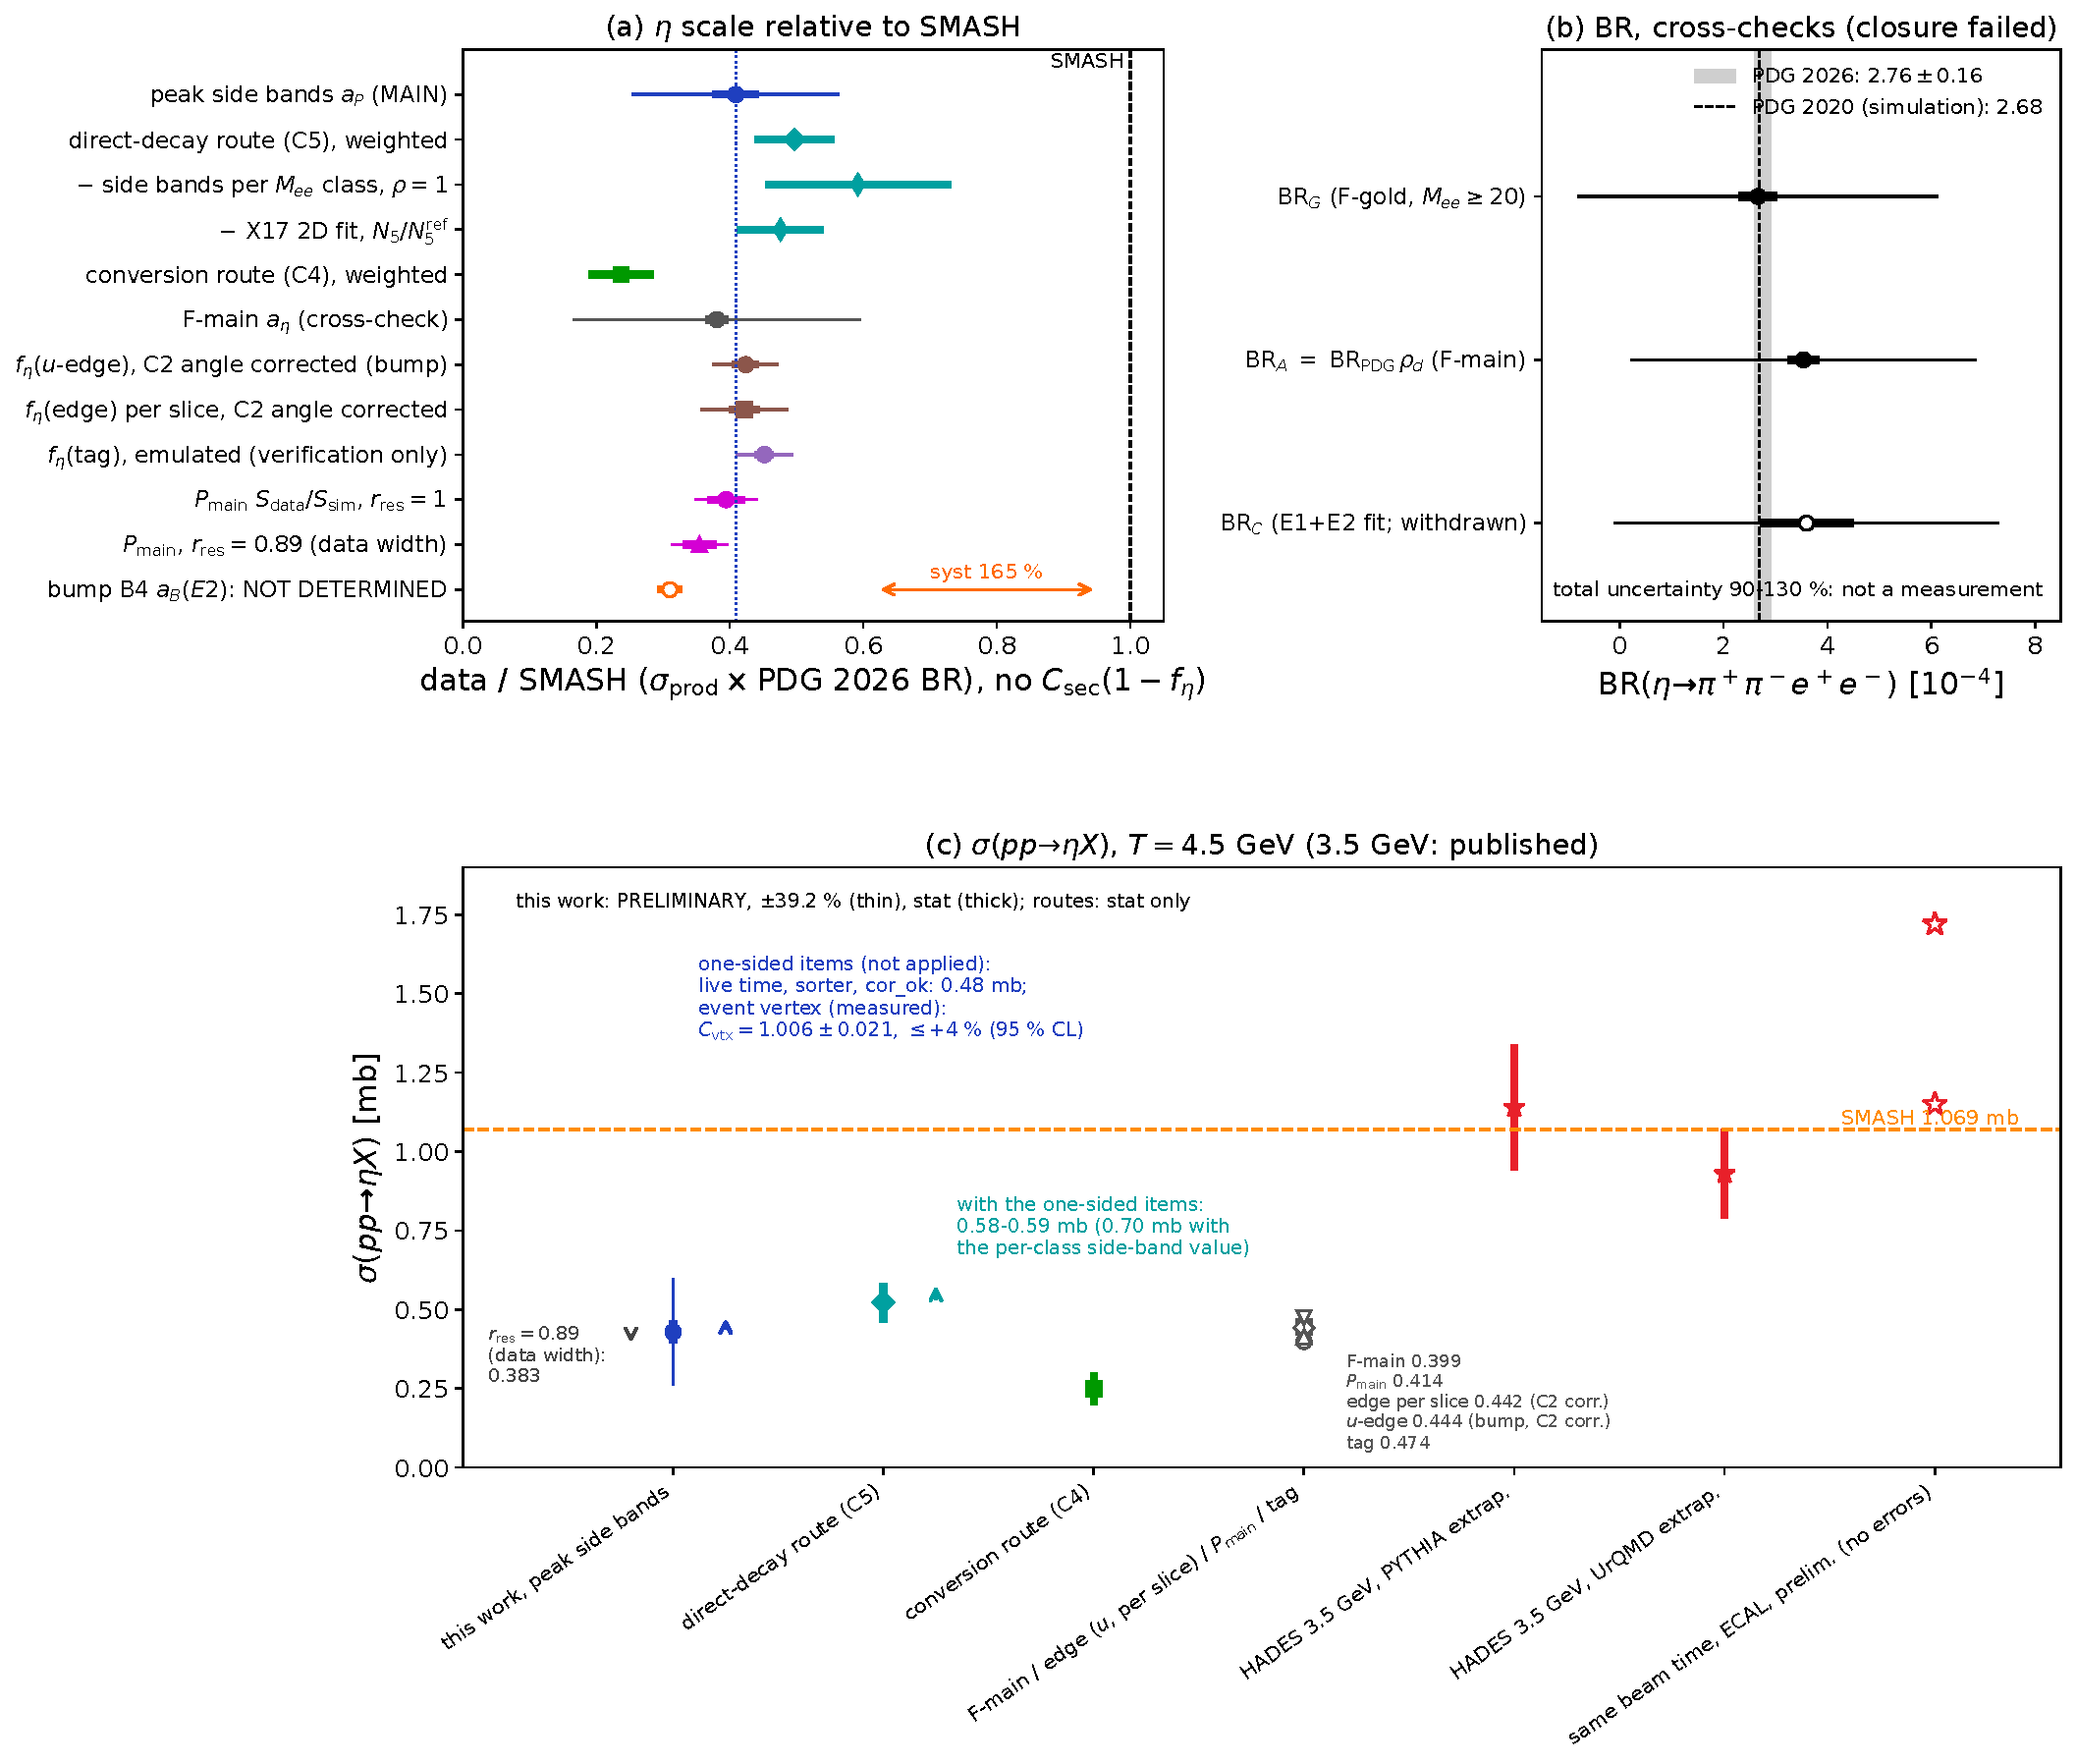
\includegraphics[width=\textwidth]{figs_all/fix2_P1abc_v4.pdf}
\caption{\textbf{What it shows: \sigeta is about 0.4 of SMASH, below the HADES values at 3.5\,GeV.}
The main estimate and the cross-checks put the data at about 0.4 of the SMASH $\eta$, and the resulting \sigeta lies below the published
HADES values at 3.5\,GeV.
Selection: data S0 (PT3 trigger, event vertex at $\vz>-160$\,mm, \betanew identification (pions $3\sigma$, leptons $5\sigma$ with a RICH ring), corrected momenta, all stored combinations (isBest $\ge0$), both pions in the event-vertex fit) and SMASH with the same cuts, each estimate in its own windows: peak side bands (peak window 0.53364--0.55416, side bands 0.5250--0.5336 and 0.5542--0.5628\,\GeVcc), its two parts also per \Mee class (below, from 10\,\MeVcc) and from the X17 fit (\Mfour 0.5225--0.6100\,\GeVcc, \Mee 2--62\,\MeVcc); template fits on \Mee$\ge10$ (F-main), $\ge20$\,\MeVcc (F-gold) or both classes (F-free), \Mfour 0.400--0.700\,\GeVcc; bump edges at $0.30\le\Mpipi<0.40$\,\GeVcc; ECAL tag $0.119\le M(\ee\gamma)<0.173$\,\GeVcc, \Mee$<0.10$\,\GeVcc; \Pmain fit in 0.5225--0.6100\,\GeVcc; B4 on \Mee$\ge10$\,\MeVcc.
The $\eta$ results at a glance. (a) $\eta$ scale data/SMASH from every estimator: the main one (peak side bands), the two parts of the
peak (direct decays, converted photons), the cross-checks, the bump through its kinematic edge (in $u$, the bump measurement, and per slice;
both with the C2 decay angle corrected) and the bump estimator B4 (not determined); thick bars statistical, thin bars total.
(b) BR$(\eta\to\ppee)$ from the template fits (cross-checks, total uncertainty 90--130\,\%) against PDG. (c) \sigeta of this work (PRELIMINARY)
with the two parts of the peak, the cross-checks (F-main 0.399, the bump in $u$ 0.444 and per slice 0.442, \Pmain 0.414, tag 0.474\,mb) and
the effect of the corrections that are not applied (arrows), against the published HADES
inclusive values at 3.5\,GeV and the unpublished values of the same beam time (open stars, no errors). Same figure as Fig.~\ref{fig:P1}, top
row, where the caption gives every detail.}
\label{fig:res-p1}
\end{figure}

%----------------------------------------------------------------------
\subsection{The \texorpdfstring{$\eta$}{eta} peak is measured}
\label{sec:res-peak}
The $\eta$ peak at \Mfour$=0.544$\,\GeVcc (Fig.~\ref{fig:res-peak}b) holds the direct decays $\eta\to\ppee$ and the decays $\eta\to\pipi\gamma$
with a converted photon. Counted as the data in the peak window minus the like-sign background and minus the smooth background taken from two side
bands (corrected for the part of the peak that leaks into them), it contains
$\Ypeak=5088\pm432\,(\mathrm{stat})\pm584\,(\mathrm{syst})\pm245\,(\mathrm{MC})$ counts (11.5\,\% systematic; 15.2\,\% if the variants that the
data reject are counted too, i.e.\ without rule R1, 14.7\,\% with the specification's literal rule), i.e.\
$\aP=0.418\pm0.035\,(\mathrm{stat})\pm0.025\,(\mathrm{MC})$ of the SMASH expectation:
the data hold about 0.4 of the $\eta$ that SMASH predicts. The other $\eta$-scale estimates agree (0.36--0.45: template fit,
ECAL tag (its simulated acceptance verified, its photon-energy scale not, \S\ref{sec:res-ecal}), Part~II's peak fit \Pmain, and the bump edge, now a measurement of its own, \S\ref{sec:res-bump}), but
they share the counts, the luminosity and the simulated efficiencies, so they are consistent, not independent confirmations.
This count is not comparable with Part~II's $S=4364\pm310\pm477$ (PEAK): Part~II fits a frozen Gaussian in another selection
and does not include the factor 64/63, so the two parts are compared through the $\eta$ scale relative to SMASH (Part~II's fit
\Pmain on S0: 0.403, or 0.363 at the data-favoured mass resolution, \S\ref{sec:sb}).
\textbf{Status:} measured. The side-band method is the only estimator that recovered the known truth on simulated pseudo-data (the test:
Fig.~\ref{fig:V1} in \S\ref{sec:val}, panel ``peak side bands''), under the rule adopted during the analysis (method configurations + RF, D22, approved by the analyst on 15 November 2026), which was chosen after the results of the specified
configuration BA were seen. Under BA every estimator failed, the peak side bands included ($+14$\,\% in one scenario); with the bootstrap bias
correction (RB) the peak side bands are ``FAIL marginal''. The method is not limited by the simulation statistics. \textbf{Details:} \S\ref{sec:sb}, \S\ref{sec:val}, \S\ref{sec:syst}.

\begin{figure}[tbp]
\centering
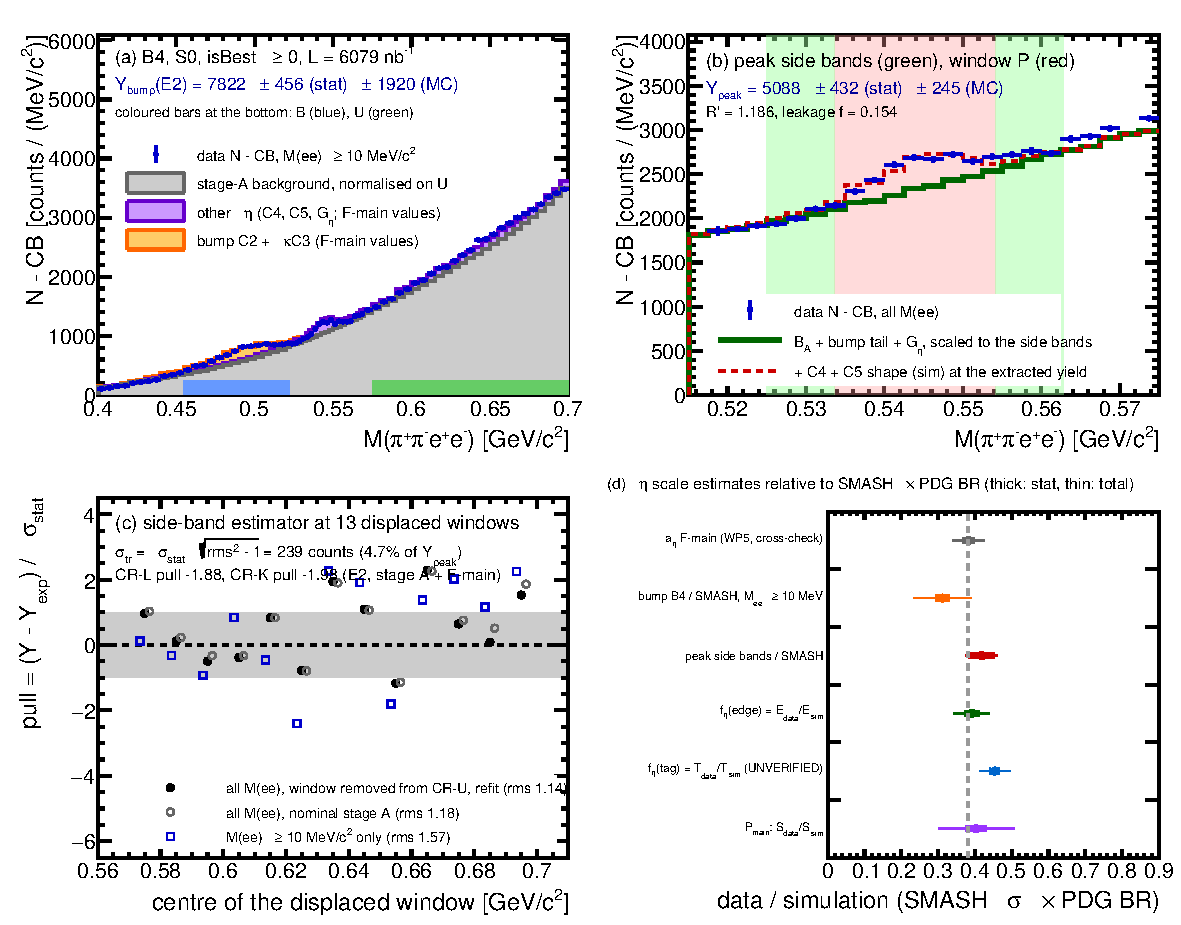
\includegraphics[width=0.80\textwidth,trim=0 222 0 0,clip]{figs_all/fix_wp6_E4_unrot_cnt.pdf}
\caption{\textbf{What it shows: a clear $\eta$ peak (b) and the bump on its carried-down background (a).}
A clear $\eta$ peak stands above a smooth background (b); the bump below it sits on a background that has to be carried down from above
the peak (a).
Selection: data S0 (PT3 trigger, event vertex at $\vz>-160$\,mm, \betanew identification (pions $3\sigma$, leptons $5\sigma$ with a RICH ring), corrected momenta, all stored combinations (isBest $\ge0$), both pions in the event-vertex fit) and SMASH with the same cuts; CB $=2\sqrt{N_{++}N_{--}}$ of the like-sign data (10\,\MeVcc cells, $k=1$), shared out by the like-sign share of each 50\,\MeVcc band. (a) \Mee$\ge10$\,\MeVcc, the five \Mpipi slices summed, bump window 0.4550--0.5225\,\GeVcc, background normalised in \Mfour 0.575--0.700\,\GeVcc; (b) all \Mee, peak window 0.53364--0.55416\,\GeVcc, side bands 0.5250--0.5336 and 0.5542--0.5628\,\GeVcc.
What the $\eta$ signal looks like in the data (selection S0, data minus the like-sign background, blue points). (a) The bump below the
peak, \Mee$\ge10$\,\MeVcc: the background (grey) is normalised to the data above the peak (green bar) and carried down into the bump window (blue
bar); violet: the other $\eta$ classes; orange: the bump at the B4 yield, which is not determined (the bump is measured through its edge
instead, \S\ref{sec:res-bump}). The legend of (a) gives the yield in this
class, $\Ybump(E2)=7822$ counts (\Mee$\ge10$\,\MeVcc); the all-\Mee value of \S\ref{sec:res-bump}, 16\,389 counts, is the E2 value divided by
the simulated E2 share, 0.477. (b) The $\eta$ peak, all \Mee: window P (red)
with its two side bands (green); green line: the background scaled to the side bands; red dashed: plus the simulated peak shape at the measured
yield. Same panels as Fig.~\ref{fig:E4}(a, b).}
\label{fig:res-peak}
\end{figure}

%----------------------------------------------------------------------
\subsection{The \texorpdfstring{$\eta$}{eta} bump is measured through its kinematic edge}
\label{sec:res-bump}
\begin{figure}[!t]
\centering
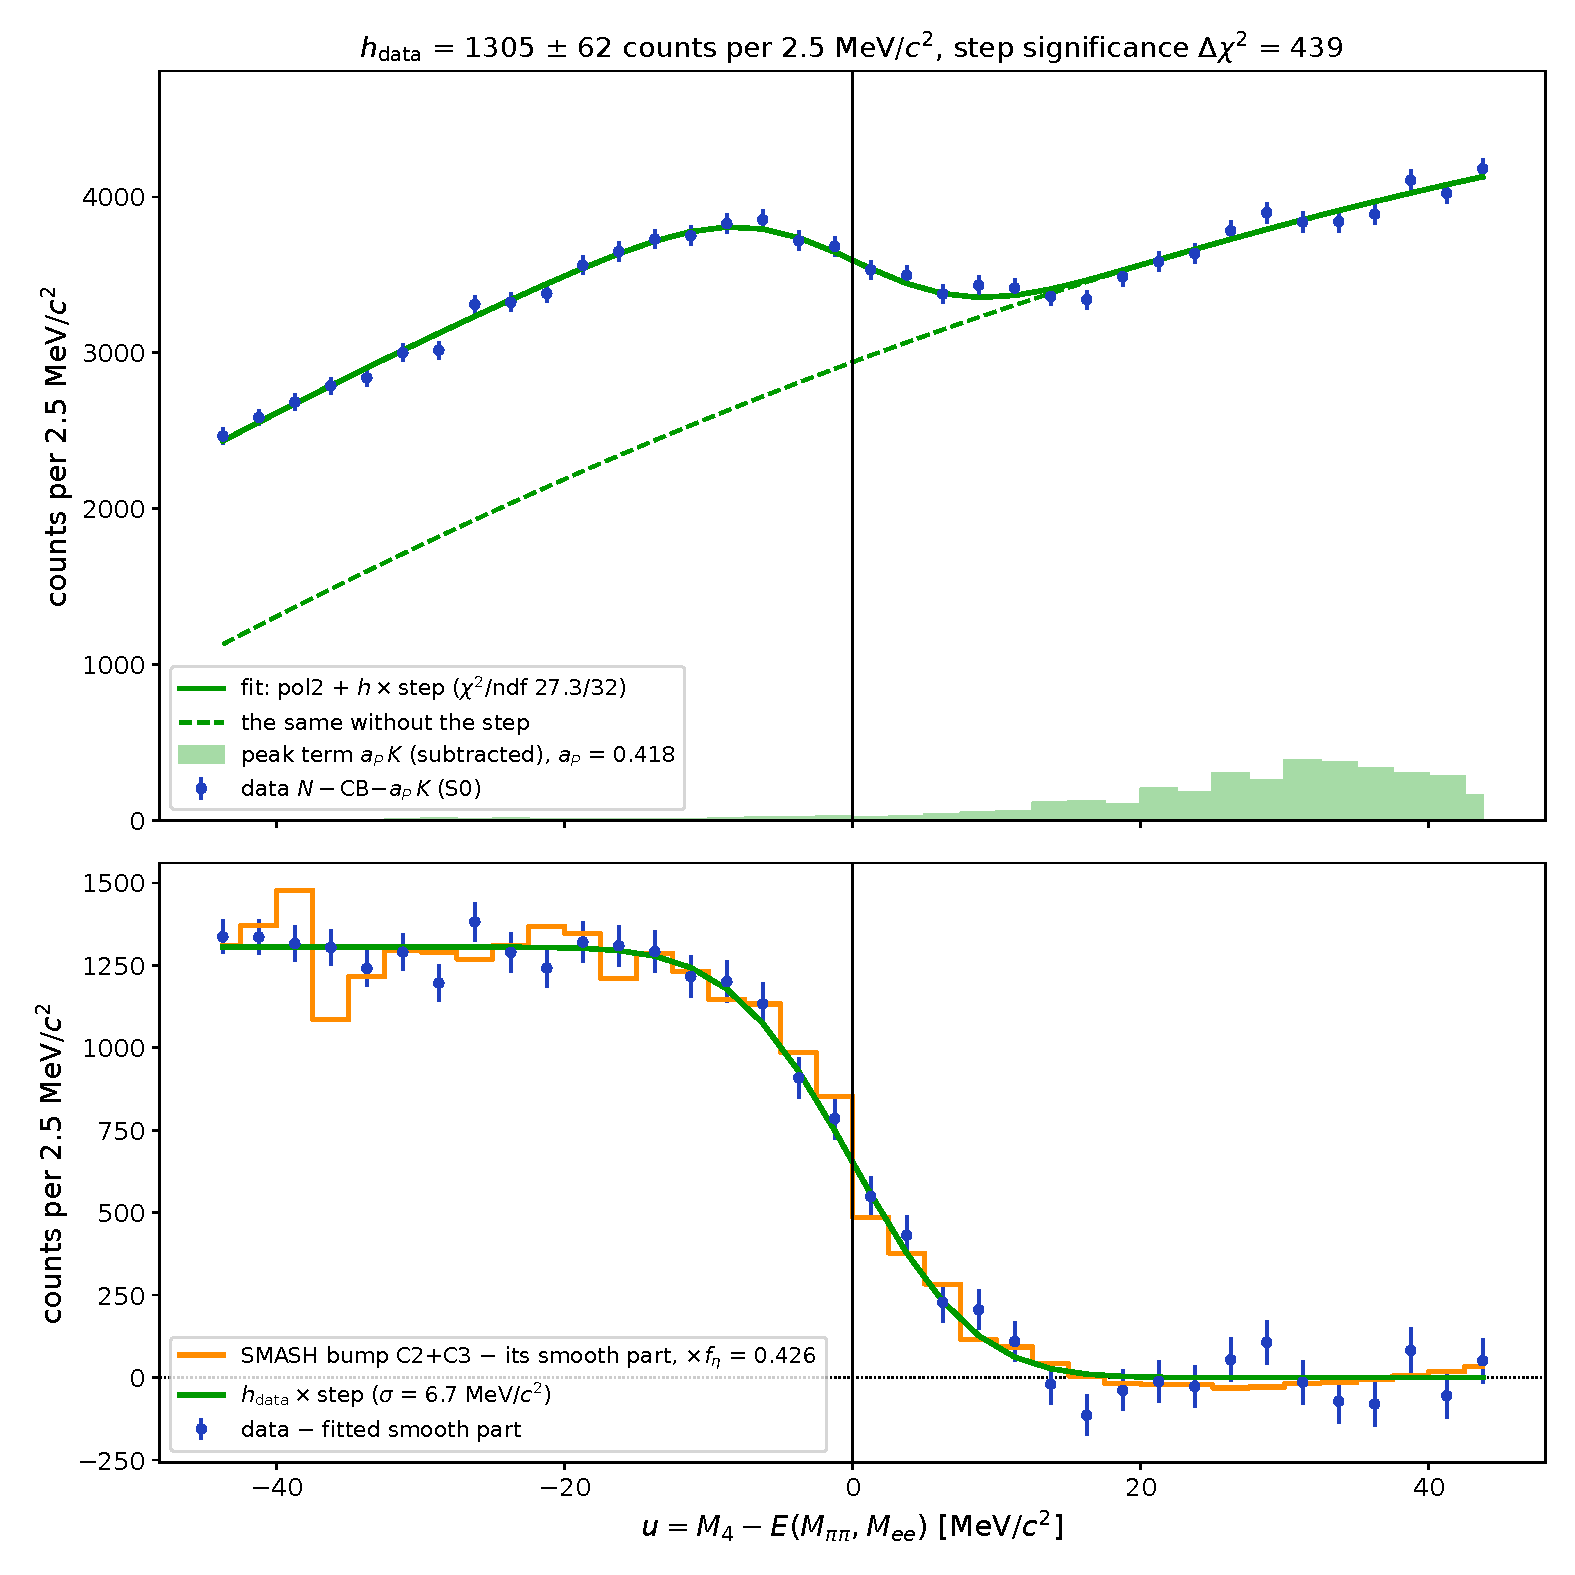
\includegraphics[width=0.78\textwidth]{figs_all/edgeu_fit_v3.pdf}
\caption{\textbf{What it shows: one fit with a smooth part and a step at $u=0$ describes the data ($\chi^2=27.3$ for 32 degrees of freedom);
the step is 21$\sigma$ and has the shape of the SMASH bump scaled by $f_\eta=0.426$.}
Selection: data S0 (PT3 trigger, event vertex at $\vz>-160$\,mm, \betanew identification (pions $3\sigma$, leptons $5\sigma$ with a RICH ring), corrected momenta, all stored combinations (isBest $\ge0$), both pions in the event-vertex fit); $0.30\le\Mpipi<0.40$\,\GeVcc, \Mee below 135\,\MeVcc (where $u$ is defined); $-45\le u<45$\,\MeVcc in 2.5\,\MeVcc bins; CB in 10\,\MeVcc cells of $u$ per \Mpipi slice (0.30--0.34, 0.34--0.37, 0.37--0.39, 0.39--0.40\,\GeVcc); SMASH peak and bump with the same cuts.
Data S0, isBest $\ge0$, $0.30\le\Mpipi<0.40$\,\GeVcc, $L=6079.2\,\nbinv$, counts per 2.5\,\MeVcc against the distance to the kinematic edge,
$u=\Mfour-E(\Mpipi,\Mee)$. Top: data $N-\mathrm{CB}-\aP K$ (blue; $K$ = SMASH peak C4+C5 in $u$, $\aP=0.418$, green area, subtracted); green
line: the fit, a second-order polynomial (the smooth part) plus $h\times$step at $u=0$; dashed: the smooth part of the same fit. The smooth part
also absorbs the slope of the bump below the edge, so the dashed line is \emph{not} the background; only the step height is a physical quantity.
Bottom: data minus the fitted smooth part (blue); SMASH bump C2+C3 (C2 with its per-count QED weights) minus its own smooth part (same fit) $\times f_\eta=0.426$ (orange);
$h_{\mathrm{data}}\times$step (green, smearing 6.7\,\MeVcc). $h_{\mathrm{data}}=1305\pm62$ counts per 2.5\,\MeVcc; without the step the fit is
worse by $\Delta\chi^2=439$. Details in \S\ref{sec:edgeu}.}
\label{fig:res-edgeu}
\end{figure}

\begin{figure}[!tbp]
\centering
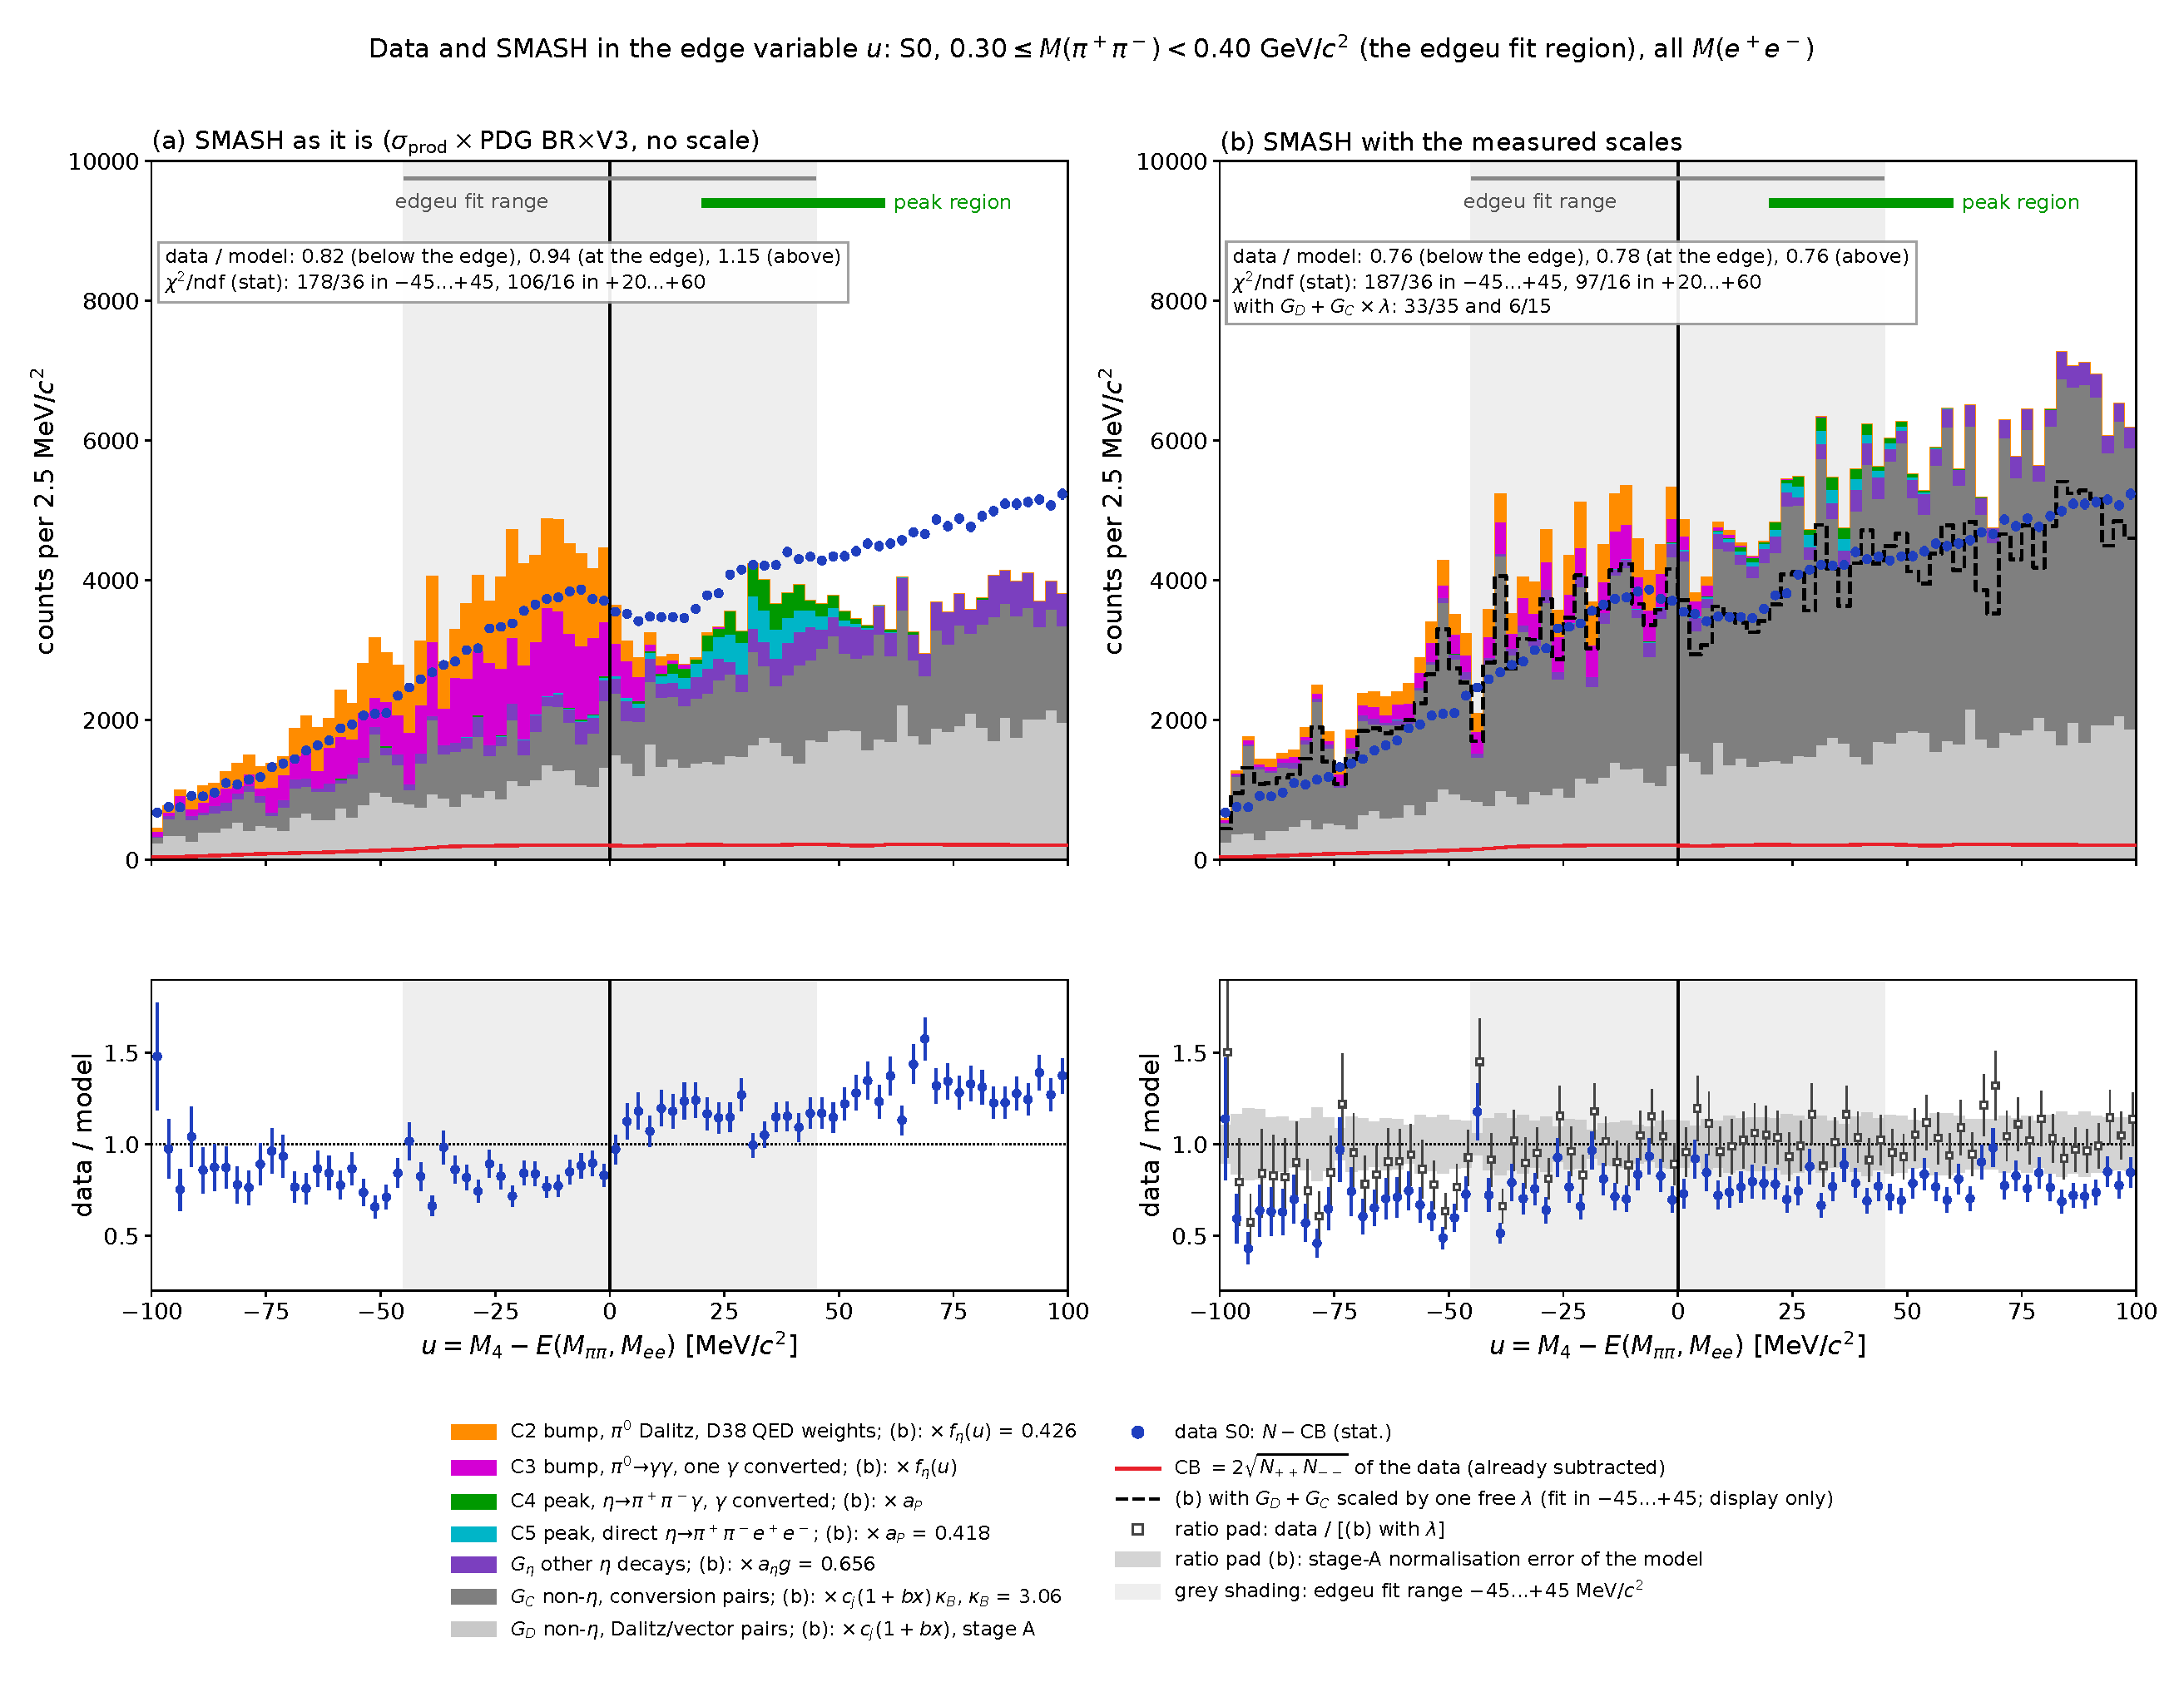
\includegraphics[width=0.94\textwidth]{figs_all/udatasim_u_overlay.pdf}
\caption{\textbf{What it shows: in the variable $u$ the data and SMASH have the same structure: one step at $u=0$ from the bump, the $\eta$ peak
at $u=+20$ to $+55$\,\MeVcc, and a smooth background that rises with $u$. With the measured $\eta$ scales (b), SMASH reproduces the position and
the width of the data step and the shape of the peak region; the step size is fixed by $f_\eta(u)$, which was fitted to these data. The one
difference beyond the statistical errors is the level of the smooth non-$\eta$ background. The normalisation of Fig.~\ref{fig:res-after} was
fitted for \Mee$\ge10$\,\MeVcc; carried to all \Mee, it puts the model 1/0.76 too high at every $u$ (1/0.65 below 10\,\MeVcc, 1/0.95 above,
within errors). This is 1.6--1.9 standard deviations of the stage-A normalisation error (grey band).}
Selection: data S0 (PT3 trigger, event vertex at $\vz>-160$\,mm, \betanew identification (pions $3\sigma$, leptons $5\sigma$ with a RICH ring), corrected momenta, all stored combinations (isBest $\ge0$), both pions in the event-vertex fit) and SMASH with the same cuts; $0.30\le\Mpipi<0.40$\,\GeVcc; ``all \Mee'' means \Mee below 135\,\MeVcc, where $u$ is defined; CB in 10\,\MeVcc cells of $u$ per \Mpipi slice 0.30--0.34, 0.34--0.37, 0.37--0.39 and 0.39--0.40\,\GeVcc.
Data S0 (isBest $\ge0$), $0.30\le\Mpipi<0.40$\,\GeVcc, all \Mee, $L=6079.2\,\nbinv$: $N-\mathrm{CB}$ in counts per 2.5\,\MeVcc (blue); CB
$=2\sqrt{N_{++}N_{--}}$ from the like-sign data (red line, already subtracted). Stack: SMASH in expected counts, C2 with the per-count QED
weights of D38; C2 orange, C3 magenta, C4 green, C5 cyan, \Geta violet, $G_C$ dark grey, $G_D$ light grey (the greys of
Fig.~\ref{fig:res-after}). Lepton pairs from the two different photons of a \piz (cross-photon pairs) are produced by SMASH but are not part of these
SMASH templates: they are left to the CB taken from the data. (a) SMASH as it is ($\sigma_{\mathrm{prod}}\times$PDG BR). (b) The measured scales: C2 and C3 $\times f_\eta(u)=0.426$;
C4 and C5 $\times\aP=0.418$; \Geta$\times\aEta g=0.656$; $G_D$ and $G_C$ $\times$ the stage-A normalisation of Fig.~\ref{fig:res-after}
($c_j(1+bx)$, $\kB=3.06$ on $G_C$); dashed: (b) with $G_D+G_C$ scaled by one free factor $\lambda=0.73$ (display only). Lower pads: data/model
with statistical errors (data and simulation); in (b) grey band: the stage-A normalisation error; open squares: data/[(b) with $\lambda$]. Light
grey shading: the $u$-edge fit range. Not to over-read: the level mismatch is statistically large ($\lambda=0.73\pm0.02$), but the stage-A error
is dominated by the MC error of \kB ($3.06\pm1.45$); $f_\eta$ takes its smooth part from the data (pol2), so this level does not enter it. The
non-$\eta$ templates are raw SMASH: a simulated conversion-background ($G_C$) count stands for about 27 expected counts, $\times3.06$ in (b), so
about 84; the spikes of the stack are this template. \Geta ($\times0.656$, not a robust scale) is 3.5\,\% of the model (5\,\% for
\Mee$\ge10$\,\MeVcc). Same figure as Fig.~\ref{fig:edgeu-sim}, where the caption gives every detail.}
\label{fig:res-udatasim}
\end{figure}

\textbf{In short:} every bump combination has a kinematic upper limit of \Mfour, its edge, set by its own \Mpipi and \Mee. In the distance to
it, $u$, all edges fall on $u=0$, and one fit finds a step of 21$\sigma$: the bump holds $0.426\pm0.049$ of the SMASH $\eta$, and the bump alone
gives \sigeta $=0.444$\,mb, as the peak does. The per-slice edge of the first revision agrees (0.423) and is the cross-check; $u$ is the bump
measurement (D37, approved by the analyst on 15 November 2026).

\textbf{What is measured, in plain words.} Below the peak, $\eta\to\pipi\piz$ in which the \piz gives an \ee pair (Dalitz decay
$\piz\to\gamma\ee$, class C2, or a converted \piz photon, class C3) and the remaining photon is lost gives a broad bump. Because a photon is
missing, the four tracks carry less mass than the $\eta$, but never more than a limit set by kinematics alone: the bump ends at a sharp upper
edge whose position is known, not fitted. The limit $E$ depends on two quantities measured in every combination: \Mpipi fixes how fast the \piz moves
in the $\eta$ frame, and \Mee how much energy the photon gets in the \piz frame (a heavier pair leaves less for the photon; Eq.~\ref{eq:edge}).
So every bump combination carries its own edge, and the distance to it, $u=\Mfour-E(\Mpipi,\Mee)$, is at most zero for every bump combination: in $u$
all edges sit on top of each other at $u=0$, and there is one sharp step. In the simulated truth no bump entry (C2 or C3) lies above its edge (largest
excess $-0.5$\,\MeVcc); without the \Mee term 3.8\,\% of C2 would. The resolution of $u$ at the edge is about 6.7\,\MeVcc in SMASH (the
template width; 5.8--7.1\,\MeVcc depending on how the core is fitted), almost all from the error of \Mfour. The step is fitted in the data with
a smooth part (a second-order polynomial) plus the step, and with exactly the same fit in SMASH; the ratio of the two step heights is the
$\eta$ scale of the bump, $f_\eta(u\text{-edge})$ (Fig.~\ref{fig:res-edgeu}). A smooth background cannot make a step; it is absorbed by the
smooth part. The first revision measured the same step in four \Mpipi slices of \Mfour, with an edge that moves inside each slice by 5--7\,\MeVcc
and ignores \Mee (the per-slice edge, Fig.~\ref{fig:res-edge}); it was Part~II's measure $E$ and is now the cross-check.

\textbf{Result.} One fit over $-45\le u<+45$\,\MeVcc gives a step of $h_{\mathrm{data}}=1305\pm62$ counts per 2.5\,\MeVcc ($\chi^2=27.3/32$);
without the step the fit is worse by $\Delta\chi^2=439$, i.e.\ 21$\sigma$. The $\eta$ peak, at $u=+20$ to $+55$\,\MeVcc, enters as a fixed
SMASH term scaled by the measured peak scale \aP; its size does not matter for the step (3.86 counts of step per unit of \aP; \aP$\pm0.08$ moves $f$ by
0.02\,\%), but its shape does: the SMASH peak has a low-mass tail that reaches $u\approx0$. The tail is the leptons' radiation in the
detector material (HGeant; the generator writes no radiative photon). Without it $f$ would be 6.9\,\% lower. A plain Gaussian peak term built
from the data (Part~II's data-only fit) gives $h_{\mathrm{data}}=1217\pm66$ and an $f$ 8.6\,\% lower (no tail, plus $-3.9$\,\% from peak positions
taken from a side-band subtraction). The data do not measure the size of the tail ($t=0.3\pm1.0$ times the simulated one); a peak without a
tail is excluded by physics, not by the data. Half the tail is a systematic term of $\pm3.4$\,\% (D40, approved by the analyst; included in the quoted error;
\S\ref{sec:edgeu-tail}). With the HGeant decay angle of class C2 corrected by per-count QED weights (\S\ref{sec:res-qed}, D35, D38):
\[ f_\eta(u\text{-edge})=0.426\pm0.020\,(\mathrm{stat})\pm0.034\,(\mathrm{syst})\pm0.030\,(\mathrm{MC})\ \text{of SMASH (11.6\,\% total)}, \]
and 0.390 without the correction. The visible bump yield in window B (all \Mee) is
$\Ybump(u)=21\,468\pm1003\,(\mathrm{stat})\pm1708\,(\mathrm{syst})\pm1347\,(\mathrm{MC})$ counts (3.53 visible counts per \nbinv). The bump alone gives
$\sigeta=0.444\pm0.021\pm0.035\pm0.031\,^{+0.043}_{-0.044}\,(\mathrm{norm.})$\,mb (0.407\,mb without the correction), next to the 0.429\,mb of the
peak (Fig.~\ref{fig:res-ecompare}). The double ratio peak/bump is $\mathrm{DR}_u=0.97\pm0.09\,(\mathrm{stat})\pm0.35\,(\mathrm{syst})\pm0.09\,
(\mathrm{MC})$, $\pm0.37$ in total, because it includes the composition term of the peak ($\pm32$\,\%): bump and peak agree, but this is a weak
test.

\textbf{Data and SMASH in $u$.} Fig.~\ref{fig:res-udatasim} puts the data and SMASH side by side in $u$. Both have the same structure: one step
at $u=0$ (the bump), the $\eta$ peak at $u=+20$ to $+55$\,\MeVcc and a smooth background that rises with $u$; no SMASH class other than the bump
has a step at $u=0$. SMASH as it is (a) does not describe the data: its bump is about 2.3 times too large, and above the peak its background is
too low, as in Fig.~\ref{fig:res-before} (data/SMASH 0.82 below the edge, 1.15 above). With the measured scales (b: the bump $\times
f_\eta(u)=0.426$, the peak $\times\aP=0.418$, the non-$\eta$ background normalised as in Fig.~\ref{fig:res-after}), SMASH reproduces the
position and the width of the step and the peak region. The size of the step is not a test, because $f_\eta(u)$ was fitted to these data. For
\Mee$\ge10$\,\MeVcc, where the background normalisation was fitted, model (b) describes the data: $\chi^2=37.0/36$ in $-45\le u<+45$\,\MeVcc
and 11.1/16 in the peak region, data/model 0.95, 0.92 and 0.95 below, at and above the edge. The only mismatch beyond the statistical errors is
the level of the smooth non-$\eta$ background for all \Mee: the model is 1/0.76 too high at every $u$ (1/0.65 below 10\,\MeVcc). The reason is
known: this normalisation (stage A, with the conversion scale $\kB=3.06\pm1.45$ on $G_C$) was fitted for \Mee$\ge10$\,\MeVcc only (stage A
dropped E1, a fall-back) and is too high when carried to small \Mee, where the conversion pairs dominate; the data there want a conversion
scale of about 1.5--1.7. Statistically the mismatch is large (one free factor on the background, $\lambda=0.73\pm0.02$, removes it), but it is
only 1.6--1.9 standard deviations of the stage-A normalisation error. $f_\eta$ is not affected: the edge fit takes its smooth part from the
data, not from SMASH (\S\ref{sec:edgeu-sim}).

\textbf{How reliable, and the doubts next to the numbers.} On pseudo-data (21 truths, 1000 toys each) the estimator recovers the truth within
$\pm2$\,\% for smooth backgrounds, with pull widths 0.95--1.07; the quadratic background term that moves B4 by $+150$\,\% moves the $u$-edge by
$-2.2$\,\% (the independent verification finds $-2.0$\,\%). Two things bias it, as they bias the per-slice edge: a mismatch of the mass resolution
between data and SMASH ($+6$\,\% in the case tested) and background structures as narrow as the edge ($+8$ and $+17$\,\% for the two
structures tested); none is seen in SMASH, and a data region without the bump shows $3\pm17$ counts of step. The systematic error is 8.0\,\%: the
data/SMASH resolution ratio (4.5\,\%), the step that a smooth background projects onto the edge (4.0\,\%, from the pseudo-data), the
low-mass tail of the peak (3.4\,\%, D40; it takes over the 0.8\,\% of the old peak-term family U8) and the combinatorial background
(2.6\,\%). Not counted, but stated: the phase-space and weights-off variants of the $\eta\to3\pi$ Dalitz plot ($+6$ to
$+8$\,\%; rejected by the KLOE-2 measurement and the WP7 rule R1; with them the systematic error would be 10.6\,\%) and the edge without the \Mee
term ($+5.9$\,\%; kinematically wrong for Dalitz pairs). The other $\eta$ decays of SMASH (\Geta) show a raw step of $123\pm53$ counts (2.3$\sigma$)
without visible structure; it is treated as template noise (if it were real, $f$ would be 3.8\,\% lower, covered in size by the 4.0\,\% item).
The four \Mpipi slices agree ($\chi^2=1.0/3$). Two checks are marginal, as they were for the per-slice edge: the data periods ($p=0.024$; period
IIB high, III low; above the WP7 limit 0.01, so no term is added) and two random halves of the data ($z=-2.1$). The MC error (7.0\,\%) is still
larger than the statistical one (4.7\,\%).

\textbf{Comparison with the per-slice edge.} Both give the same scale (0.426 and 0.423) and the same \sigeta (0.444 and 0.442\,mb). The total
error is 11.6\,\% against 15.4\,\% as quoted for the per-slice edge, but most of this gain comes from taking the simulated step from the bump
classes alone, which the per-slice method can also do (then about 6.6\,\% MC and about 12.4\,\% total, both with the peak tail). The gain that
belongs to $u$ itself is about 12.4 $\to$ 11.6\,\%, with a statistical error about 8\,\% smaller (4.77\,\% against 5.19\,\%). The model dependence is not smaller: both methods rest
on the resolution matching and on the step that a smooth background projects onto the edge. Four separate fits in $u$, one per slice, give the
same numbers ($0.429\pm0.020\pm0.032$).

\textbf{A step in the like-sign counts, explained (D39).} The like-sign counts from which the combinatorial background is built were expected to
show no edge. The $e^-e^-$ counts nevertheless show a step of $73.5\pm15.7$ at $u=0$ (4.7$\sigma$); through CB $=2\sqrt{N_{++}N_{--}}$ the
subtracted CB carries 39 counts of it (3\,\% of $h_{\mathrm{data}}$). A dedicated study (package eestep) found the mechanism, and it is physics:
the step counts are pairs of leptons from the \emph{two different photons} of the \piz in $\eta\to\pipi\piz$ (a Dalitz $e^-$ and a conversion
$e^-$ of the other photon, or two conversion $e^-$; ``cross-photon pairs''). For a given \Mee such pairs have exactly the same kinematic edge
$E(\Mpipi,\Mee)$ as the bump (a toy of $4\times10^5$ decays never exceeds $u=0$), and near the edge they are heavy. The data show exactly this
(Fig.~\ref{fig:res-eestep}): the $e^-e^-$ step is $57.0\pm9.1$ counts (6.3$\sigma$) at \Mee$\ge90$\,\MeVcc and $3.6\pm8.9$ (none) below
50\,\MeVcc, where 90\,\% of the bump lies; the two leptons are 20--60$^\circ$ apart; the step follows $E$ with its \Mee term ($\Delta\chi^2=28.3$,
0.5 without the \Mee term) and sits at $u=0$ (free position $-2.5$\,\MeVcc); 85\,\% of these counts come from events with no positive lepton at all.
They are seen mostly as $e^-e^-$ for two reasons: soft $e^+$ are accepted less often than soft $e^-$, and a photon can also give a Compton or
knock-on electron, which is always negative (SMASH contains such pairs, mostly $e^-e^-$); at \Mee$\ge90$\,\MeVcc the $e^+e^+$ counts do have a
step, $7.3\pm4.3$ (ratio to $e^-e^-$ $0.13\pm0.08$); ``the $e^+e^+$ counts have no step'' ($2.1\pm6.5$ over all \Mee) was a statement about
small numbers. A decay with a Dalitz or conversion pair on each photon
gives one $e^-e^-$, one $e^+e^+$ and two $e^+e^-$ cross pairs; a Compton or knock-on electron gives one $e^-e^-$ and one $e^+e^-$ pair; with
an acceptance that factorises per lepton the CB rule removes both from $N$ to within a few per cent. The data confirm
it at \Mee$\ge90$\,\MeVcc, where the bump is small: the step of $N$ is $52.6\pm10.9$ counts, the CB step $35.8\pm8.6$, and
$N-\mathrm{CB}=16.8\pm13.9$ against $16.9$ expected from the bump (SMASH $\times f$, a signal prediction); if the like-sign step were an artefact
without $e^+e^-$ partners, $N-\mathrm{CB}$ would be $-19.0$, 2.6$\sigma$ away (statistical; somewhat less with the error of the simulated bump,
17 simulated entries). The scale of the cross pairs in $N$ relative to the CB rule, from the data, is $k_{\mathrm{cross}}=1.00\pm0.39$ (about
$\pm0.5$ with the CB-step and simulation errors; independent check, made with the earlier constant C2 factor, $0.96\pm0.48$). A charge flip of the Dalitz $e^+$ (the reading of the first note) would put the step at the small \Mee of the
bump, where there is none: flip rate $<1.2$\,\% (90\,\% CL; simulation 0.01--0.04\,\% per pair).

\textbf{What it means for the numbers.} Nothing changes: $f_\eta(u\text{-edge})=0.426$ and the per-slice 0.423 are right as they stand. Using
$k_{\mathrm{cross}}$ instead of 1 moves $f(u)$ by $0.0\pm1.2$\,\% (inside the CB systematic U5, 2.6\,\%; not a new term); an $e^+$ flip at its
90\,\% CL limit would raise $f$ by less than 1.6\,\% (1.9\,\% for a flip of either charge). The earlier caveat ``$f$ could be higher by up to
about 8\,\%'' is withdrawn. \Ypeak is not affected (cross pairs reach the peak window only at \Mee$\ge102$--120\,\MeVcc and are subtracted with
their partners), nor is the X17 limit (below \Mee$=24.5$\,\MeVcc their edge stays 11--12.5\,\MeVcc below the peak window). No merged conversion pairs are seen.
\textbf{Status:} D39, proposed by the lead analysis (record the origin, keep the CB and U5), approved by the analyst on 15 November 2026;
confirmed by an independent verifier (wording corrected: the Compton and knock-on electrons, the size of the CB test). \textbf{Details:} \S\ref{sec:edgeu-ls}.

\begin{figure}[!tbp]
\centering
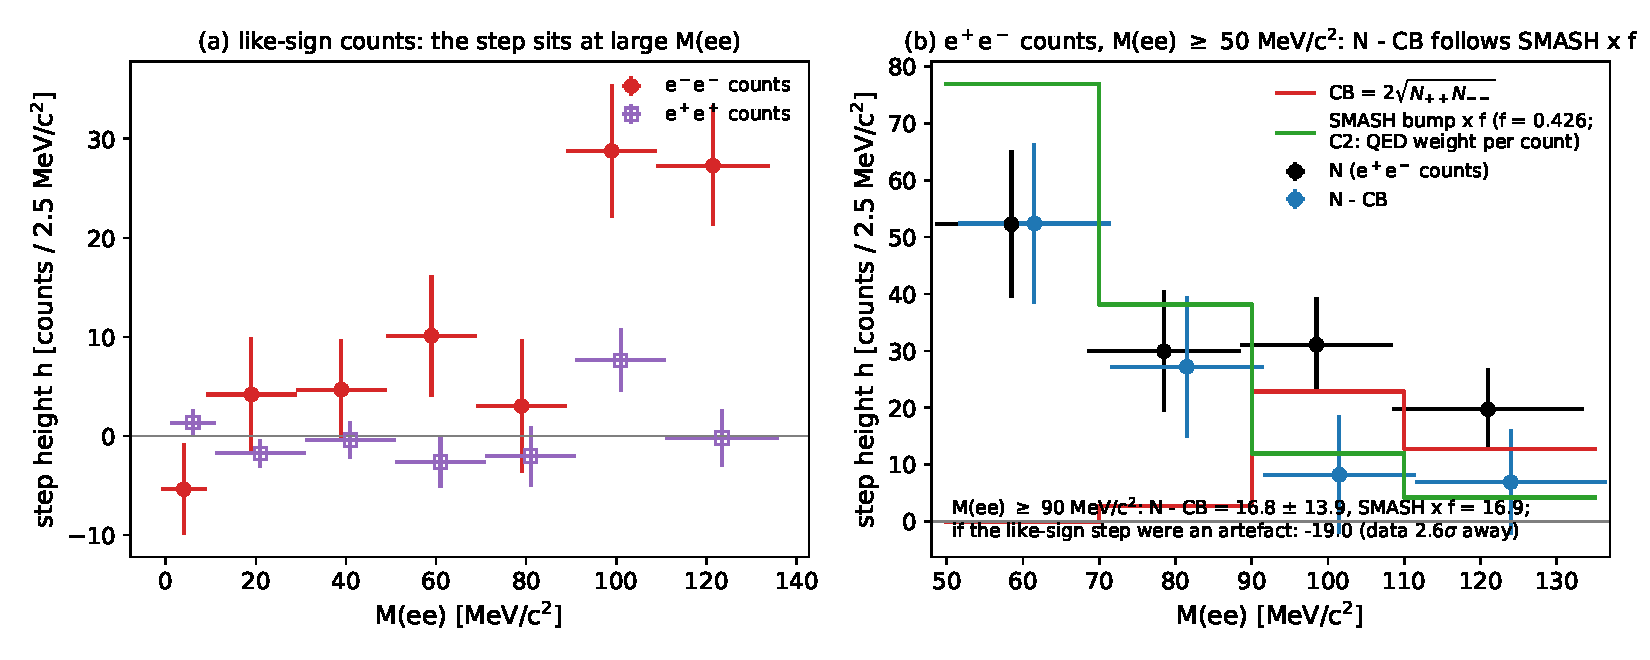
\includegraphics[width=\textwidth]{figs_all/eestep_bands_v3.pdf}
\caption{\textbf{What it shows: the step of the like-sign counts at the bump edge sits at large \Mee, where lepton pairs from the two \piz photons
lie; there the unlike-sign counts carry the matching step, so $N-\mathrm{CB}$ follows the expected bump signal and the CB rule is right.}
Selection: data S0 (PT3 trigger, event vertex at $\vz>-160$\,mm, \betanew identification (pions $3\sigma$, leptons $5\sigma$ with a RICH ring), corrected momenta, all stored combinations (isBest $\ge0$), both pions in the event-vertex fit); $0.30\le\Mpipi<0.40$\,\GeVcc; step of the nominal $u$-edge fit in the \Mee bands 0--10, 10--30, 30--50, 50--70, 70--90, 90--110 and 110--135\,\MeVcc ((b): from 50\,\MeVcc; ``\Mee$\ge90$\,\MeVcc'' means 90--135\,\MeVcc); (a) like-sign counts alone, no CB subtracted; (b) CB from the like-sign counts of the same band; SMASH bump with the same cuts.
Data S0, $0.30\le\Mpipi<0.40$\,\GeVcc, step height $h$ at $u=0$ (counts per 2.5\,\MeVcc) of the nominal $u$-edge fit, per \Mee band.
(a) Like-sign counts of the data: $e^-e^-$ (red points) and $e^+e^+$ (violet open squares); no step below 50\,\MeVcc, a step at
\Mee$\ge90$\,\MeVcc in both (ratio $0.13\pm0.08$). (b) Unlike-sign counts at \Mee$\ge50$\,\MeVcc: $N$ (black),
the CB of each band (red line), $N-\mathrm{CB}$ (blue) and the expected bump signal, SMASH bump $\times f$ with the per-count C2 weights,
$f=0.426$ (green line). At \Mee$\ge90$\,\MeVcc
$N-\mathrm{CB}=16.8\pm13.9$ against 16.9; a like-sign artefact without $e^+e^-$ partners would give $-19.0$ (2.6$\sigma$ away, statistical).
Package eestep, independently verified (\S\ref{sec:edgeu-ls}).}
\label{fig:res-eestep}
\end{figure}

\textbf{The converted photons.} If the simulated conversion pairs are scaled by 0.48, as the peak data indicate (a documented, flexible use of
SMASH), the $u$-edge gives $0.549\pm0.026\pm0.055\pm0.037$ and $\sigeta=0.573$\,mb (per slice 0.569 and 0.594\,mb), against $0.522\pm0.062$\,mb
from the direct decays of the peak. The bump's own split into \Mee classes gives $\kappa=0.83\pm0.20\,(\mathrm{stat})\pm0.34\,(\mathrm{MC})$ in $u$
($0.47\pm0.24\pm0.46$ per slice): consistent with 1 and with the peak value 0.48, far too imprecise to choose. The bump moves together with the
peak; it does not settle the make-up question.

\textbf{The C2 correction factor at the edges (D35, D38).} The constant factor of D35 (0.881 effective, from toys and the closure) was checked
against a per-count average of the QED weight along the circle on which each lost photon must lie: the step fits need 0.861 ($u$) and 0.860
(per slice), so the constant factor left $f$ and \sigeta from the bump 1.4\,\% ($u$) and 1.2\,\% (per slice) too low. The analyst approved the
per-count weights on 15 November 2026 (D38), to be applied until a future simulation corrects the angle in GEANT itself (not expected); all
bump-edge numbers above use them ($f_\eta(u\text{-edge})=0.426$, \sigeta from the bump 0.444\,mb, 0.573\,mb with the conversions $\times0.48$),
and the model allowance is $\pm0.004$ instead of $\pm0.024$. An independent verifier rebuilt the weights with own code and confirms the factors to
within 0.0004 (\S\ref{sec:c2recon}).

\textbf{The per-slice edge (cross-check).} In four \Mpipi slices of \Mfour, with the C2 decay angle corrected, the step gives
$f_\eta(\mathrm{edge})=0.423\pm0.023\pm0.038\pm0.048$ (15\,\%; 0.392 uncorrected), $\Ybump(\mathrm{edge})=21\,445\pm1152\pm1900\pm2223$ counts
(as is), \sigeta $=0.442\pm0.024\pm0.040\pm0.050\,^{+0.042}_{-0.044}$\,mb (0.409 uncorrected) and
$\mathrm{DR}_{\mathrm{edge}}=0.97\pm0.10\pm0.17\pm0.12$ (24\,\%, without the composition term of the peak; with it about $\pm0.37$, as
DR$_u$) (Figs.~\ref{fig:res-edge}, \ref{fig:res-bscales}). It recovers 16\,000 pseudo-data sets within 2\,\% (4\,\% with noisy replica
templates), and the quadratic term moves it by $-2.1$\,\%. Its MC error (0.042, twice the statistical one; 0.038 from an independent replica set)
comes mostly from the raw simulated background in its simulated step (with bump-only templates it would be about 6.6\,\%); counted, the
two Dalitz-plot variants would raise its systematic error from 8.9 to 11.3\,\%; the two halves of the data differ at $p=0.05$ (marginal).

\textbf{What failed.} Only the background-subtracted \emph{area} under the bump (estimator B4: 16\,389 counts, 157\,\% systematic) is not
determined, because its background can only be extrapolated 40--120\,\MeVcc from above the peak: a quadratic term moves it by $+150$\,\%, and below
the bump the extrapolation already overshoots the data (Fig.~\ref{fig:res-after}). The ECAL-tagged scale, $0.454\pm0.043$, lies between the
readings and stays verification only; the full reconstruction with the ECAL photon is a feasibility study: data/expected $1.16\pm0.21$ to
$0.84\pm0.15$, depending on the photon-energy scale (\S\ref{sec:res-ecal}).
\textbf{Status:} measured; the analyst approved the C2 convention (D35) and, on 15 November 2026, $u$ as the bump measurement (D37), the
per-count C2 weights (D38), the handling of the like-sign step (D39) and the peak-tail term (D40); \sigeta from the bump inherits the PRELIMINARY label of
Part~III. \textbf{Details:} \S\ref{sec:edgeu}, \S\ref{sec:bedge}, \S\ref{sec:b4}.

\begin{figure}[!tbp]
\centering
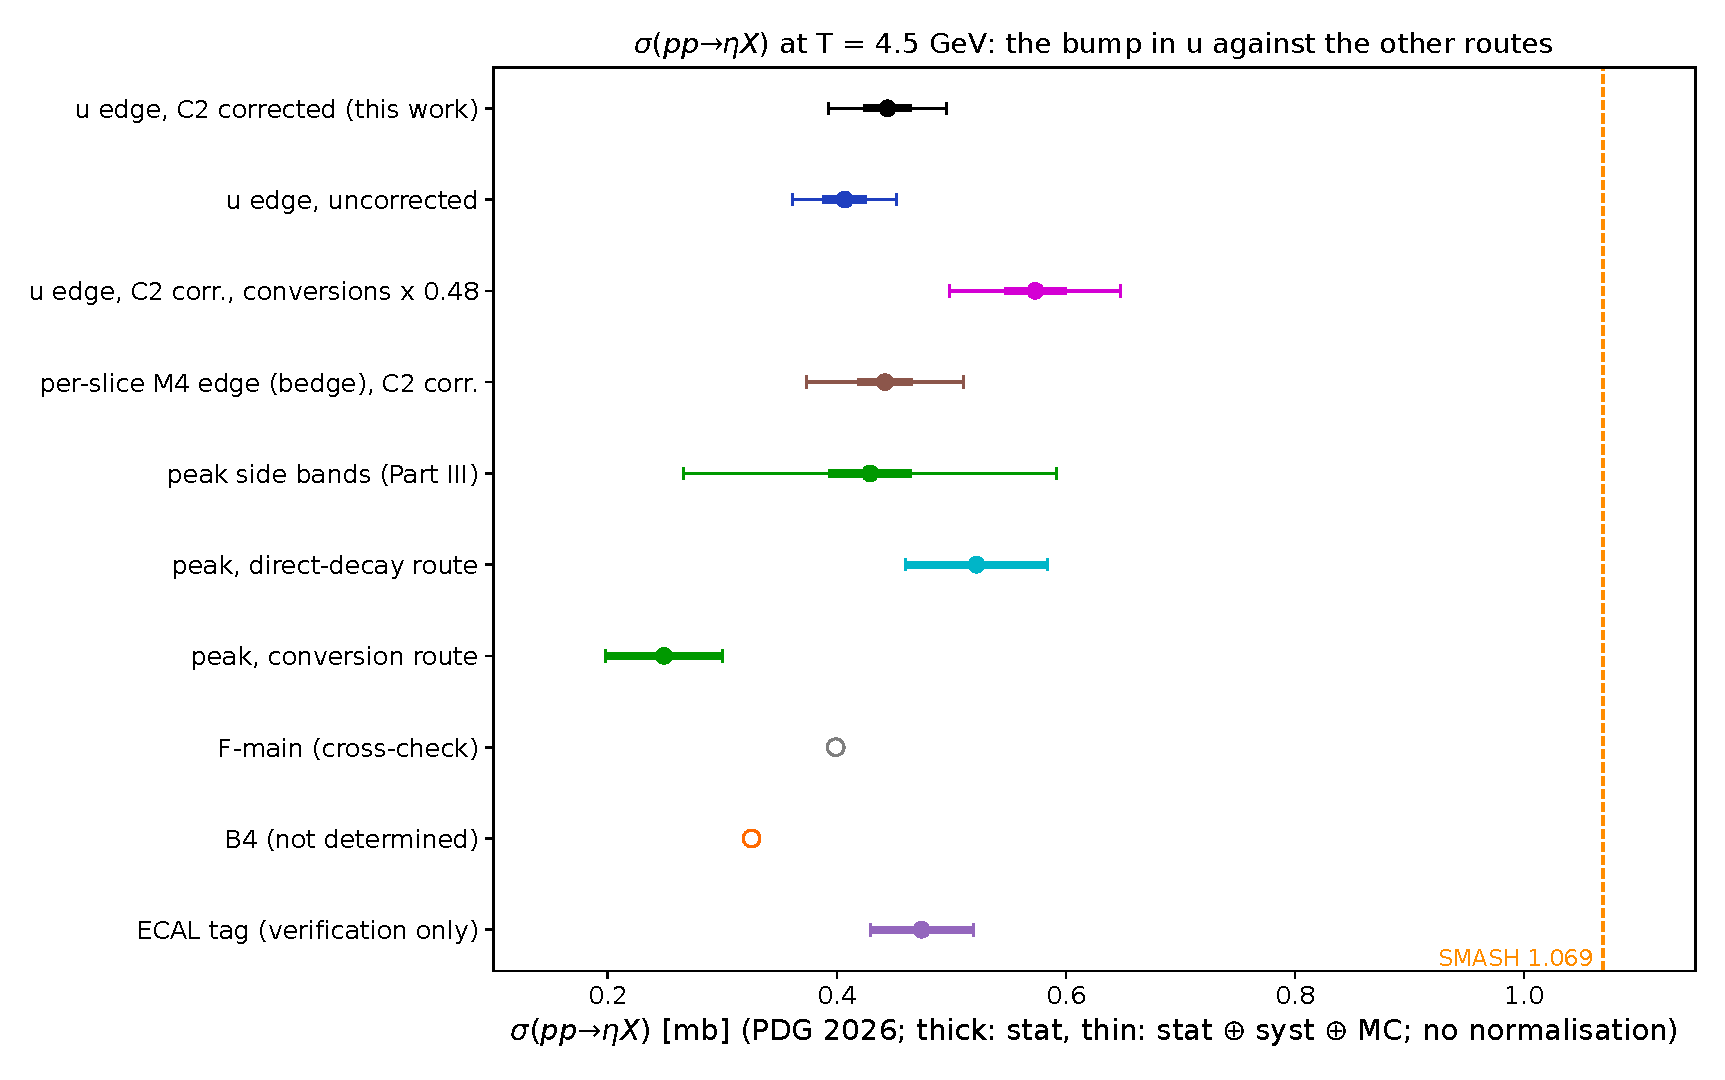
\includegraphics[width=0.86\textwidth]{figs_all/edgeu_compare_v3.pdf}
\caption{\textbf{What it shows: \sigeta from the bump in $u$ (0.444\,mb) agrees with the per-slice edge and with the peak side bands; all routes
lie a factor 2--2.5 below SMASH.}
Selection: data S0 (PT3 trigger, event vertex at $\vz>-160$\,mm, \betanew identification (pions $3\sigma$, leptons $5\sigma$ with a RICH ring), corrected momenta, all stored combinations (isBest $\ge0$), both pions in the event-vertex fit) and SMASH with the same cuts, each value in its own windows: the bump in $u$ ($0.30\le\Mpipi<0.40$\,\GeVcc, \Mee below 135\,\MeVcc (where $u$ is defined)) and per slice (the four \Mpipi slices 0.30--0.34, 0.34--0.37, 0.37--0.39, 0.39--0.40\,\GeVcc, all \Mee); peak side bands (peak window 0.53364--0.55416, side bands 0.5250--0.5336 and 0.5542--0.5628\,\GeVcc) and its routes (per \Mee class, below and from 10\,\MeVcc; X17 fit in \Mfour 0.5225--0.6100\,\GeVcc, \Mee 2--62\,\MeVcc); F-main and B4 on \Mee$\ge10$\,\MeVcc; ECAL tag $0.119\le M(\ee\gamma)<0.173$\,\GeVcc, \Mee$<0.10$\,\GeVcc.
PDG 2026; $\Csec(1-\feta)=1.0104\times0.97$ for the bump, 0.981 for the peak; thick bars: stat; thin: stat $\oplus$ syst $\oplus$ MC; the
normalisation ($^{+0.043}_{-0.044}$\,mb for the $u$-edge) is not included. From the top: the $u$-edge with the C2 decay angle corrected (per-count
weights, D38), uncorrected, and
with the conversions $\times0.48$; the per-slice edge (cross-check); the peak side bands (adopted, PRELIMINARY; total including the composition
term) and the two routes of the peak (stat only); open circles: values without errors (F-main, cross-check; B4, not determined); the ECAL tag
(verification only). Dashed: SMASH, 1.069\,mb. The one-sided items (live time, sorter, \code{cor_ok}, vertex, production model) are not
included.}
\label{fig:res-ecompare}
\end{figure}

\begin{figure}[!tbp]
\centering
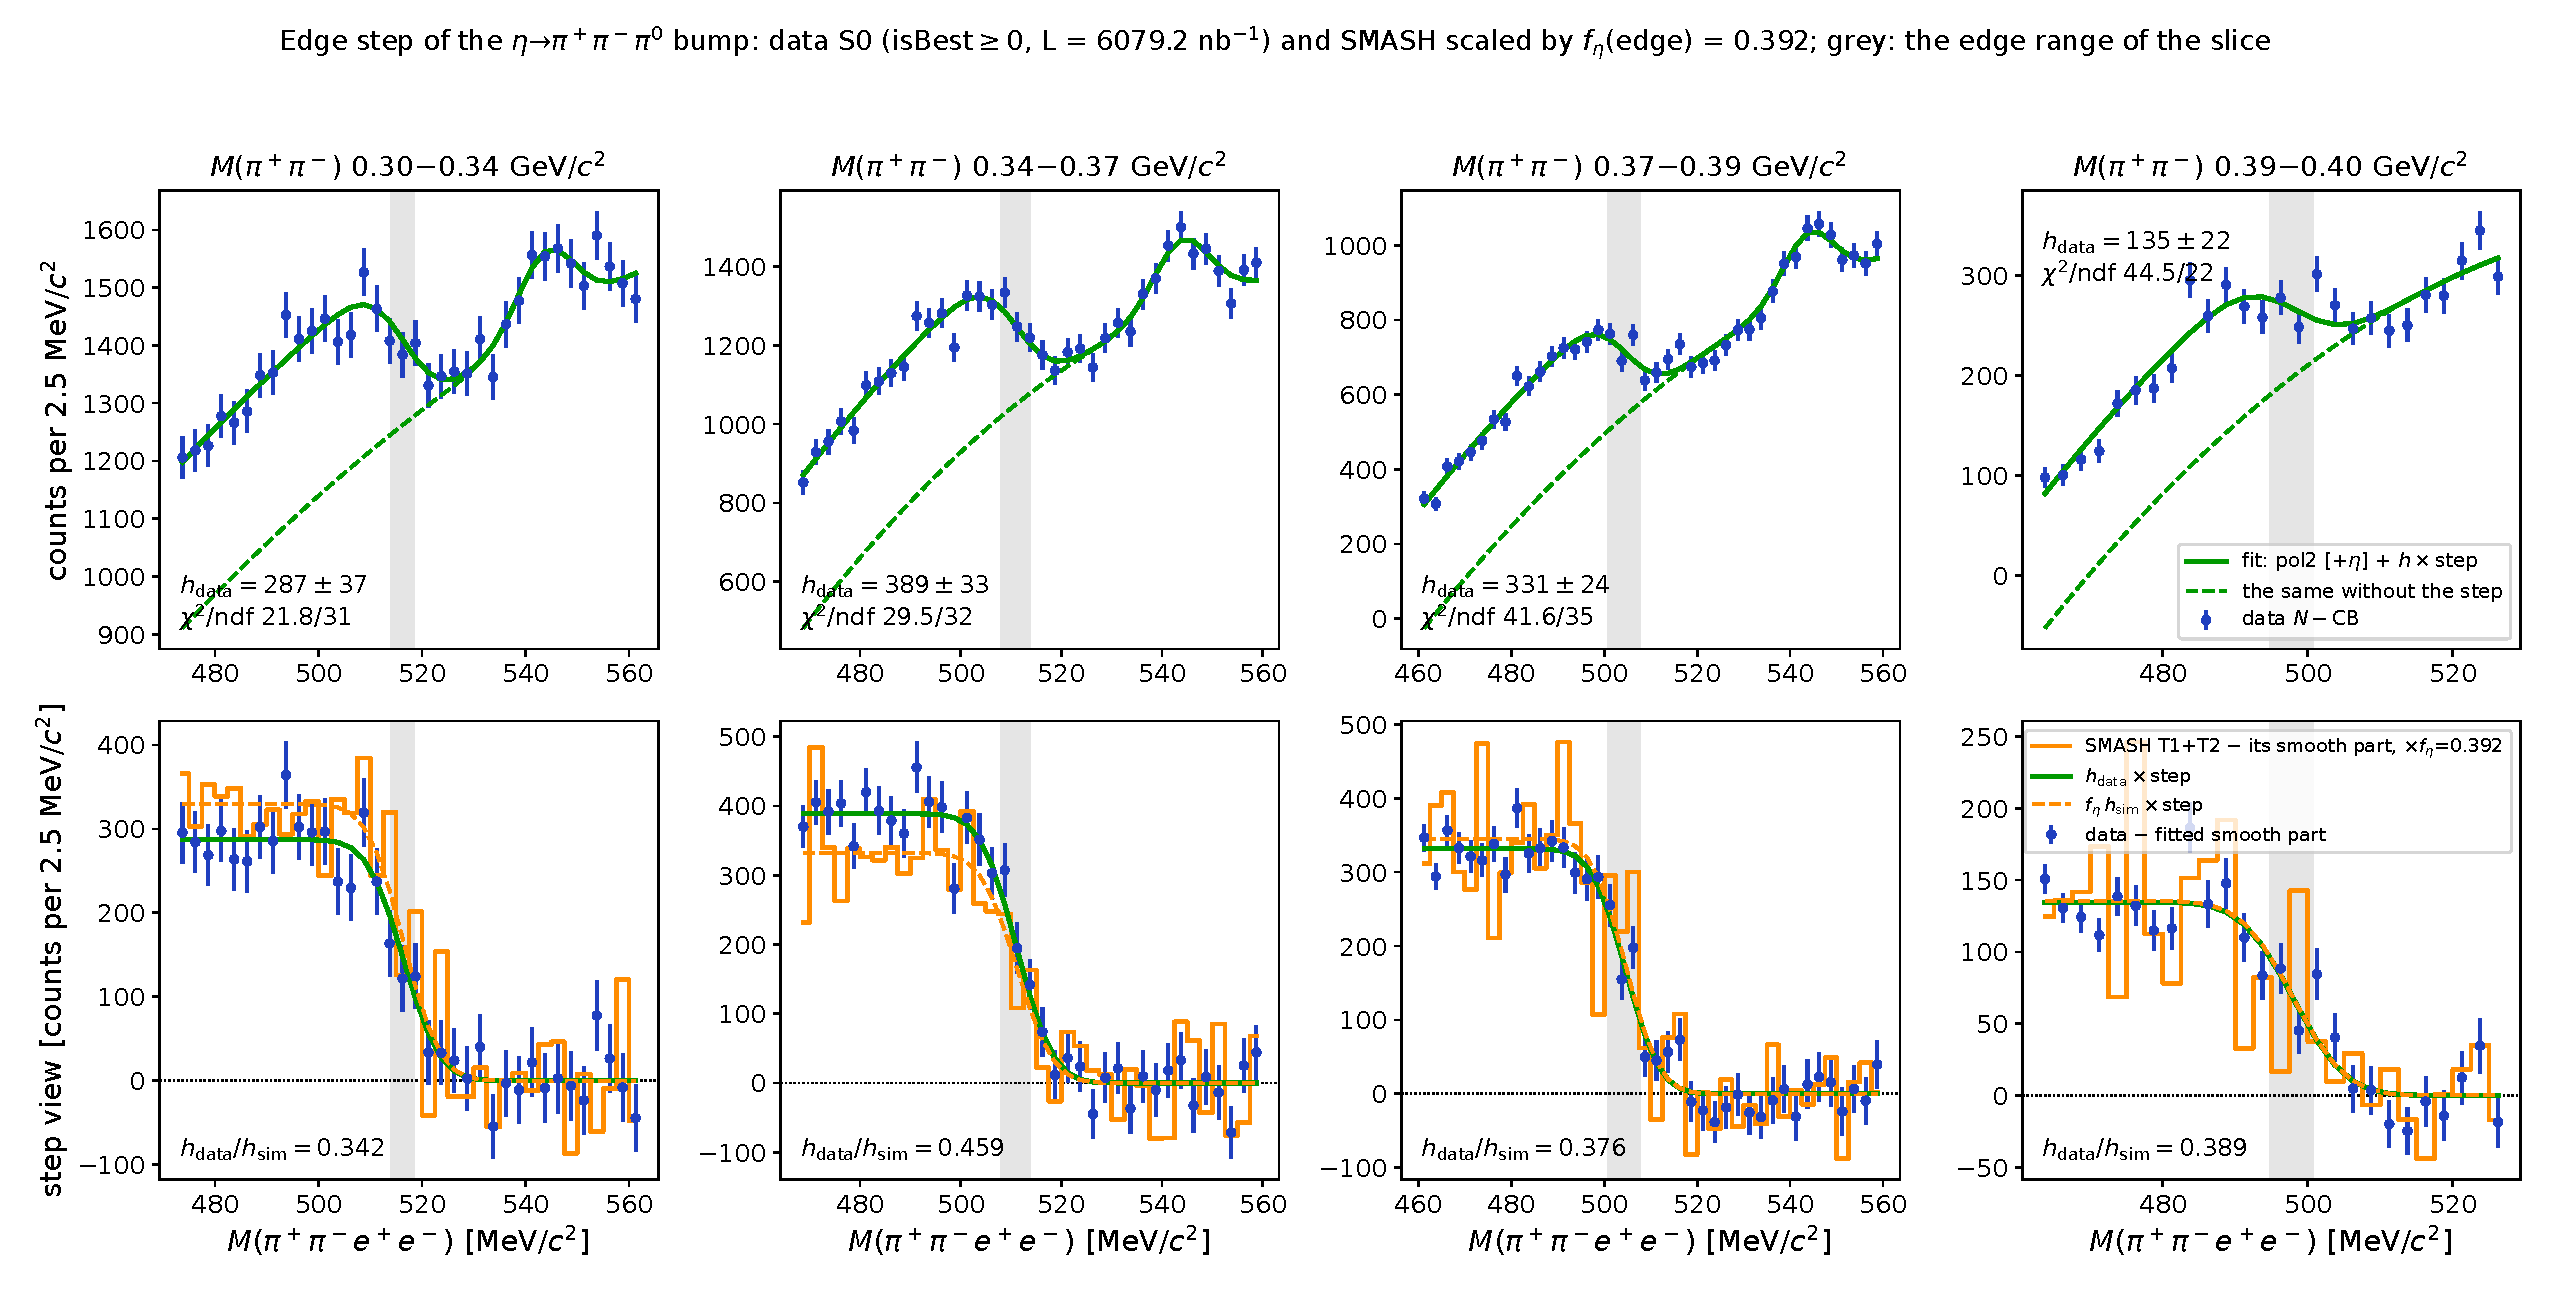
\includegraphics[width=\textwidth]{figs_all/bedge_steps_cnt.pdf}
\caption{\textbf{What it shows: the per-slice cross-check: the edge of the bump is seen in every \Mpipi slice of \Mfour, and its height in the
data is 0.39 of SMASH with the same shape.}
Selection: data S0 (PT3 trigger, event vertex at $\vz>-160$\,mm, \betanew identification (pions $3\sigma$, leptons $5\sigma$ with a RICH ring), corrected momenta, all stored combinations (isBest $\ge0$), both pions in the event-vertex fit), all \Mee, in the four \Mpipi slices 0.30--0.34, 0.34--0.37, 0.37--0.39, 0.39--0.40\,\GeVcc; fit range the edge $\pm45$\,\MeVcc ($\pm35$\,\MeVcc in 0.39--0.40); CB from the like-sign counts of each slice; SMASH $T_1+T_2$ with the same cuts and the same fit.
Data S0, isBest $\ge0$, $L=6079.2\,\nbinv$. Top: $N-\mathrm{CB}$ (blue points; CB $=2\sqrt{N_{++}N_{--}}$ of the slice) per 2.5\,\MeVcc in
the four \Mpipi slices 0.30--0.34, 0.34--0.37, 0.37--0.39 and 0.39--0.40\,\GeVcc, with the frozen fit (green): pol2 [+ $\eta$ Gaussian 0.5439 /
5.4\,\MeVcc] + $h\times$step at the edge fixed from kinematics, $0.99277\,M_4^{\max}(\Mpipi/0.9970)$, smeared by 5.4\,\MeVcc; dashed: the same
without the step. Bottom: ``step view'' $=$ data minus the fitted smooth part (blue); SMASH $T_1+T_2$ (expected raw counts, $w\times$V3,
$M_4'=0.99615\,M_4$) minus its own fitted smooth part, $\times f_\eta(\mathrm{edge})=0.392$ (orange histogram; its bin-to-bin noise is the
template statistics); green: $h_{\mathrm{data}}\times$step; orange dashed: $f_\eta h_{\mathrm{sim}}\times$step. Grey band: the edge range of the
slice. The figure shows the uncorrected ratio (same fit on both sides); with the C2 decay angle corrected the scale is 0.423 (per-count weights, D38). Details in
\S\ref{sec:bedge}; the earlier display of the same fit is Fig.~\ref{fig:edge}.}
\label{fig:res-edge}
\end{figure}


\begin{figure}[!tbp]
\centering
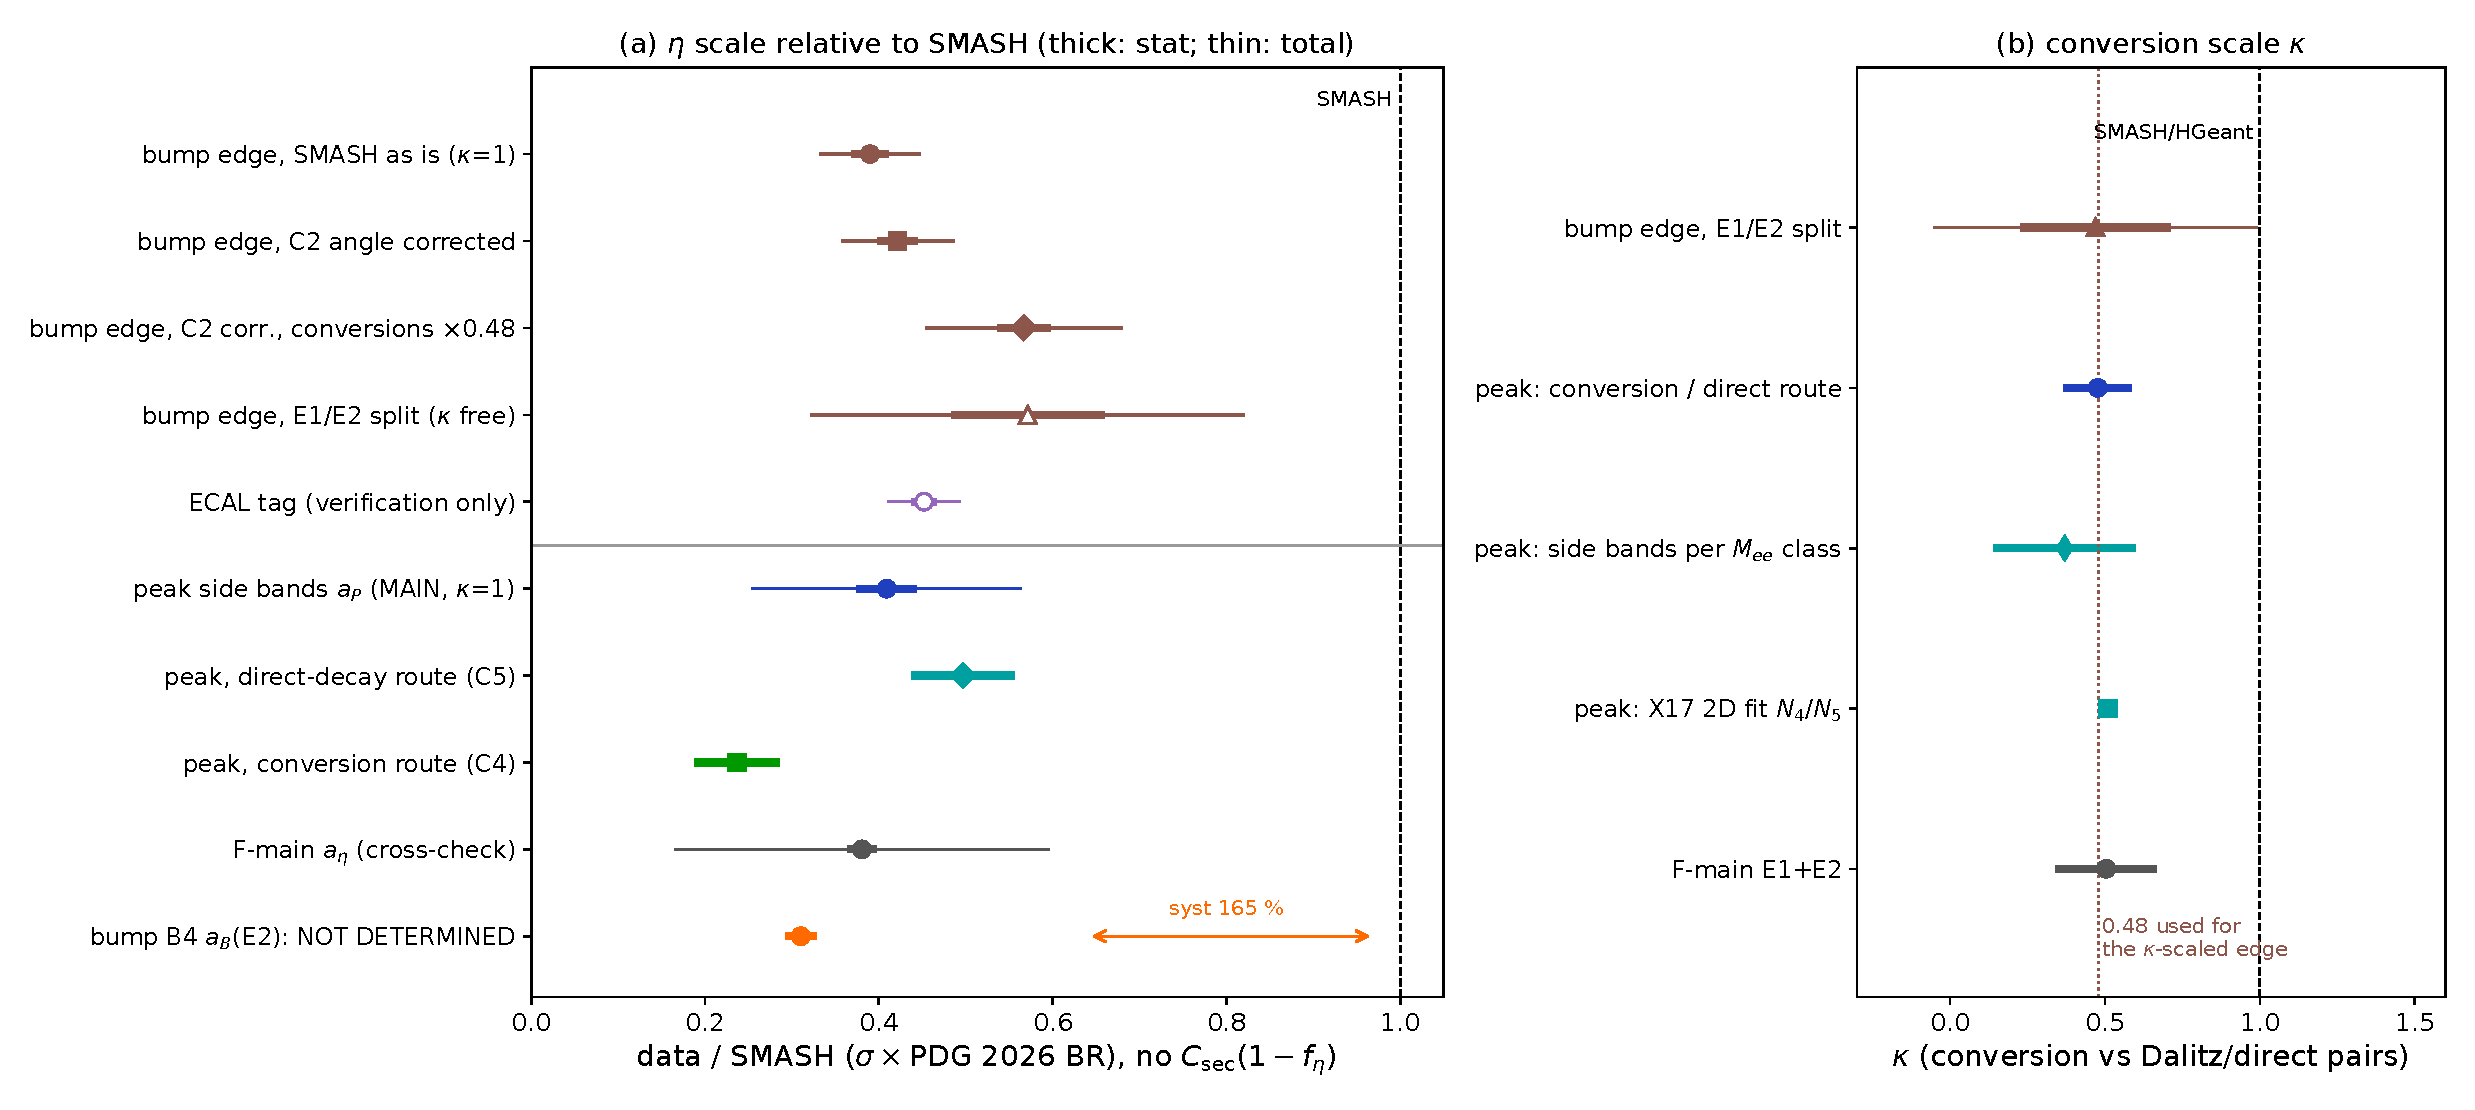
\includegraphics[width=\textwidth]{figs_all/bedge_scales_v3.pdf}
\caption{\textbf{What it shows: the per-slice bump edge gives the same $\eta$ scale as the peak, 0.39--0.42 of SMASH with the simulated
conversion rate, and 0.57 if the conversion pairs are scaled by 0.48 as the peak data indicate.}
Selection: data S0 (PT3 trigger, event vertex at $\vz>-160$\,mm, \betanew identification (pions $3\sigma$, leptons $5\sigma$ with a RICH ring), corrected momenta, all stored combinations (isBest $\ge0$), both pions in the event-vertex fit) and SMASH with the same cuts, each value in its own windows: per-slice edge in the four \Mpipi slices 0.30--0.34, 0.34--0.37, 0.37--0.39, 0.39--0.40\,\GeVcc (all \Mee; with $\kappa$ free, \Mee below and from 10\,\MeVcc); ECAL tag $0.119\le M(\ee\gamma)<0.173$\,\GeVcc, \Mee$<0.10$\,\GeVcc; peak side bands (0.53364--0.55416; 0.5250--0.5336 and 0.5542--0.5628\,\GeVcc; also per \Mee class); X17 fit (\Mfour 0.5225--0.6100\,\GeVcc, \Mee 2--62\,\MeVcc); F-main (\Mee$\ge10$\,\MeVcc, for $\kappa$ both classes) and B4 (\Mee$\ge10$\,\MeVcc).
The $u$-edge (not drawn here) gives 0.426, 0.549 with the conversions $\times0.48$, and $\kappa=0.83\pm0.20\pm0.34$ from its own \Mee split
(\S\ref{sec:edgeu}).
(a) Data/SMASH ($\sigma\times$PDG 2026 BR, without $\Csec(1-\feta)$). Brown: the bump edge as is ($\kappa=1$), with the C2 decay angle
corrected (per-count weights, D35, D38), C2 corrected with the conversions $\times0.48$, and with $\kappa$ free (\Mee split E1/E2; open marker: stat and
robust MC only); violet open circle: ECAL tag (verification only); blue: peak side bands \aP (total including the composition term of the
peak, $\pm32$\,\%, and the peak tail of D40); cyan and green: the direct-decay and conversion routes of the peak (stat only); grey: F-main (cross-check); orange: B4 (not
determined, syst 165\,\%). Thick bars: stat; thin: stat $\oplus$ syst $\oplus$ MC. (b) Conversion scale $\kappa$ from the bump's E1/E2 split
and from the peak (ratio of its routes, side bands per \Mee class, X17 2D fit (drawn without its error), F-main E1+E2). Dotted: the 0.48 used for
the $\kappa$-scaled edge; dashed: SMASH.}
\label{fig:res-bscales}
\end{figure}

%----------------------------------------------------------------------
\subsection{Can the bump be reconstructed in full with the ECAL photon?}
\label{sec:res-ecal}
\textbf{In short:} one third of the lost bump photons hit an active ECAL module, and about 12\,\% of the bump can be reconstructed in full, as a
clean peak. The data hold $1.16\pm0.21$ to $0.84\pm0.15$ of the prediction, depending on the assumed photon-energy scale. It is a feasibility
study, not yet a measurement: the photon itself (energy scale, module efficiency, a START-free cut) limits it, not the statistics.

\begin{figure}[!tbp]
\centering
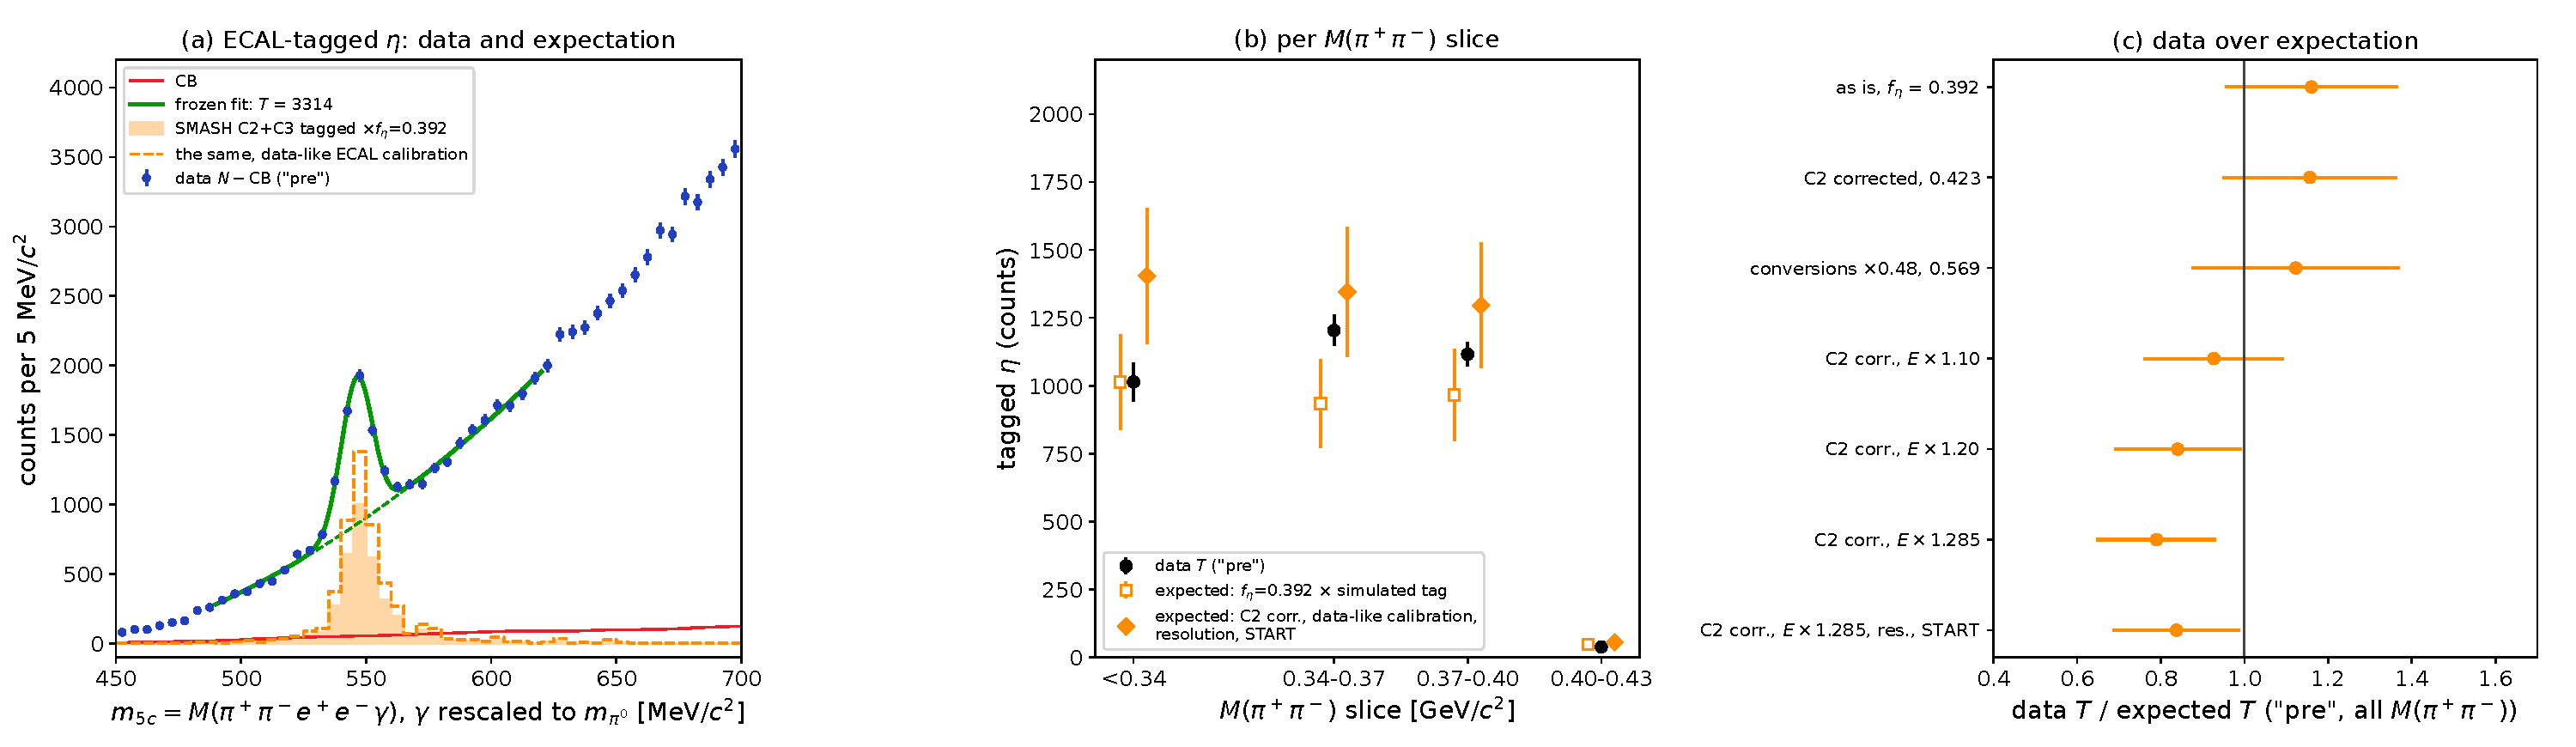
\includegraphics[width=\textwidth]{figs_all/ecalacc_tag_v3.pdf}
\caption{\textbf{What it shows: the number of ECAL-tagged $\eta$ in the data agrees with the $\eta$ scale of the bump edge within the errors, but
the prediction moves by almost 50\,\% with the assumed photon-energy scale of the 100\,MeV threshold.}
Selection: (a), (c) data ``pre'' (PT3 trigger, event vertex at $\vz>-160$\,mm, \betanew identification (pions $3\sigma$, leptons $5\sigma$ with a RICH ring), corrected momenta, all stored combinations (isBest $\ge0$), no pion-vertex condition), all \Mfour and \Mpipi, with a good ECAL photon (identified as a photon, $0.8<\beta<1.2$, above 100\,MeV), $0.119\le M(\ee\gamma)<0.173$\,\GeVcc and \Mee$<0.10$\,\GeVcc; $m_{5c}$ fitted in 0.49--0.62\,\GeVcc; (b) the same in the \Mpipi slices below 0.34, 0.34--0.37, 0.37--0.40 and 0.40--0.43\,\GeVcc. Expectation: the simulated bump C2+C3 with the same cuts and photon tag in the simulated ECAL, $\times f_\eta$.
(a) Data ``pre'', tagged counts: $N-\mathrm{CB}$ in $m_{5c}=M(\ppee\gamma)$ with the photon rescaled to $M(\ee\gamma)=m_{\piz}$ (blue; CB red), with the
frozen fit (green; $T=3314$); orange area: the simulated tagged C2+C3 entries $\times f_\eta(\mathrm{edge})=0.392$; orange dashed: the same with a
data-like ECAL energy scale. (b) $T$ per \Mpipi slice: data (black), the expectation $f_\eta\times$ simulated tag (open squares) and the best
expectation (C2-corrected $f_\eta=0.423$, cluster energies $\times1.285$, data resolution $\times0.964$, START $\times0.978$; diamonds); errors of
the expectation: stat $\oplus$ syst $\oplus$ MC of $f_\eta$ and the MC of the simulated tag (overestimated, both from the same simulated entries).
(c) Data $T$ over the expected $T$ (all \Mpipi) for the readings of the $\eta$ scale and the assumed photon-energy scales.}
\label{fig:res-ecal}
\end{figure}

\textbf{What was done.} The ECAL tag of Part~II ($T$) counts the bump combinations in which the ECAL sees the lost photon, so that the whole
$\eta\to\pipi\piz$ is reconstructed ($M(\ee\gamma)$ at the \piz mass, $m_{5c}$ at the $\eta$ mass). The simulation does not store the lost
photon, but it can be recovered: the four charged momenta, the \piz mass and the $\eta$ mass leave the photon on a known circle, along which
the SMASH $\eta$ spectrum gives the density. So every simulated bump entry gets the direction and energy of its photon, and the ECAL geometry and
module status of the simulation say whether the photon hits an active module. The 598 photons that the ECAL simulation did find lie on their
predicted circles, 99.5\,\% of them in the predicted active modules.

\textbf{The acceptance is known.} The ECAL has 6 sectors of 163 modules; ECAL sector 0 (azimuth 63--117$^\circ$; not the tracking sector 2 of
the trigger deficit) is switched off, and 8 further modules are dead, identically in the data (all four periods) and in the simulation. Seen
from the target centre the modules span 10.9--45.6$^\circ$ in polar angle; the active ones cover 8.45\,\% of the full solid angle. Of the lost
photons of the accepted bump combinations, 9.0\,\% fly below the ECAL, 54.5\,\% into its polar band and 36.5\,\% above it (9.9\,\% backward); 32.7\,\% hit
an active module, at every \Mpipi. The photon is soft (mean 130\,MeV, half of them below 100\,MeV), softest near the edge, so after the
100\,MeV cluster cut and the cluster efficiency 9.8\,\% of the bump combinations are fully reconstructed in the simulation (14.1\,\% at a data-like
energy scale); the tagged ones sit preferentially below the edge (27.5\,\% more than 60\,\MeVcc below it, against 16.5\,\% of all bump
combinations). The tag is specific to the bump: 12.7\,\% of the bump combinations are tagged, 0.8\,\% of C4 and 1.8\,\% of C5.

\textbf{Data against the prediction.} The data contain $T=3314\pm105$ tagged $\eta$ (``pre''). The prediction is the $\eta$ scale of the bump
edge times the simulated tag. As simulated it is $2857\pm153\,(\mathrm{stat})\pm234\,(\mathrm{syst})\pm400\,(\mathrm{MC})$, so data/expected
$=1.16\pm0.21$. But the photon-energy scale differs between data and simulation: in the data the cluster energy is about 17\,\% too high (the
median factor that brings $M(\ee\gamma)$ of the tagged $\eta$ to the \piz mass is 0.856), in the simulation 7--9\,\% too low (median
$E_{\mathrm{cluster}}/E_{\mathrm{true}}=0.914$ for the found photons, 0.931 after the quality cuts, from the cluster truth). The 100\,MeV cut
therefore sits near 85\,MeV true energy in the data and near 108\,MeV in the simulation. With the simulated cluster energies $\times1.285$
(data-like), the wider \piz of the data ($\times0.964$) and the loss of tags in events without a START hit ($\times0.978$) the expectation is
$3957\pm213\pm356\pm566$ and data/expected $=0.84\pm0.15$ (with the per-slice $f_\eta=0.423$; 0.83 with the $u$-edge value). These errors
are overestimated, because the MC errors of $f_\eta$ and of the simulated tag come from the same simulated entries. Per \Mpipi slice the ratio of the tag to the edge is one common factor (1.10--1.19), not a change of shape
(Fig.~\ref{fig:res-ecal}).

\textbf{What it means.} A full reconstruction with the ECAL photon keeps about 12\,\% of the bump, but as a clean peak: its statistical error is
3.2\,\% against 5.4\,\% for the edge. It is limited by the photon, not by the statistics: the prediction moves by a factor 1.46 with the energy
scale at which the 100\,MeV threshold acts, so today the tag tests the $\eta$ scale only to about $\pm20$\,\%. Before it can be a measurement the
analysis needs (1) the photon energy scale and resolution in data and simulation; (2) the module efficiency against the photon energy (inside
the active modules the ECAL simulation finds only about 65\,\% of the photons, not explained); (3) a $\beta$ cut on the photon that does not
depend on START, or a simulated START efficiency; (4) at least 10 times more simulated $\eta\to\pipi\piz$. The acceptance itself is known. This
connects with the separate ECAL analysis of D32 (new calibration). \textbf{Status:} feasibility, verification only. \textbf{Details:}
\S\ref{sec:ecalacc}.

%----------------------------------------------------------------------
\subsection{X17: no signal, and an upper limit}
\label{sec:res-x17}
A narrow \ee line of mass 10--40\,\MeVcc inside the $\eta$ peak, as $\eta\to\pipi X17$, $X17\to\ee$ would give, was searched for with a fit of
\Mfour$\times$\Mee in which the background is measured in every \Mee bin from the \Mfour side bands. The procedure was fixed on the \Mee side
bands and sealed (md5) before the data in 12--28\,\MeVcc were opened. No signal is seen (largest local excess $0.98\sigma$, at 22\,\MeVcc, Fig.~\ref{fig:X34}a in \S\ref{sec:x17};
Fig.~\ref{fig:res-x17spec}). The
90\,\% CL$_s$ upper limit at 17\,\MeVcc is
\[ r_{\mathrm{UL}}=0.114,\qquad \BRX<3.16\times10^{-5}, \]
i.e.\ X17 makes at most 11\,\% of the direct decays $\eta\to\ppee$. The limit on $r$ does not depend on the PDG edition; the absolute value
uses the PDG 2026 BR$(\eta\to\ppee)=(2.76\pm0.16)\times10^{-4}$ (ruling D25; footnote~\ref{fn:x17pdg} gives the value of the frozen
procedure, with the PDG 2020 BR fixed before the unblinding). The expected limit is $2.7\times10^{-5}$ ($\pm1\sigma$: 1.5--4.9$\times10^{-5}$), so the data lie where
the no-signal hypothesis puts them; over 10--40\,\MeVcc the limit runs from $4.0\times10^{-5}$ to $0.9\times10^{-5}$ (Fig.~\ref{fig:res-x17}). A
vector-like X17 gives $3.79\times10^{-5}$, the normalisation that the specification's fall-back would make primary $3.29\times10^{-5}$ (D30,
approved: normalisation (1) primary, (2) quoted next to it). The template statistics give an 11\,\% uncertainty of the limit, quoted apart; the simulation replicas suggest that the
nominal is about 6\,\% optimistic ($3.35\times10^{-5}$). A simple one-window count (ROOT \code{TRolke}) gives only $<2.6\times10^{-4}$: the shape
fit is about 8 times (8.3) stronger because it measures the background instead of predicting it.
The expectation of Part~I ($1.9\times10^{-5}$) assumed that the data hold all the $\eta$ that SMASH predicts and used a counting
window; it is not like-for-like and is quoted for comparison only (\S\ref{sec:x17d}).
\textbf{Status:} measured with the frozen procedure (normalisation (1) primary, (2) quoted next to it; D30, approved); blind in the code, not in the
information (Part~II had shown the \Mee shape of the peak band before the freeze; it showed no excess). \textbf{Details:} \S\ref{sec:x17},
\S\ref{sec:trolke}.

\textbf{Comparison with other searches} (Table~\ref{tab:x17cmp}; details in \S\ref{sec:x17other}). Two earlier searches exist in this channel.
Near 17\,\MeVcc the limit of this report is about two times weaker than the BESIII limit ($3.16\times10^{-5}$ against
$0.048$--$0.053\times3.07\times10^{-4}\approx1.5\times10^{-5}$) and numerically similar to the HADES preliminary value from the same beam time
($2.58\times10^{-5}$). The results are built differently: CL$_s$ here against a Bayesian limit at BESIII (a flat-prior Bayesian limit on the
likelihood of this report is $4.10\times10^{-5}$), a finer mass grid (0.5--1 against 5\,\MeVcc), $\eta$ from p+p collisions instead of $J/\psi$
decays, both the spin-0 and the vector-like hypotheses, and a procedure frozen before the unblinding. The similarity to the HADES preliminary
value is numerical only: that value comes from an event count with the Rolke method, while this report's own one-window count with
\code{TRolke} gives $<2.6\times10^{-4}$ (\S\ref{sec:trolke}), about 10 times weaker ($2.6\times10^{-4}/2.58\times10^{-5}\approx10$). The window,
background and normalisation of the preliminary count are not documented in this report, so the agreement of the two numbers is not a
cross-check.

\begin{table}[H]
\centering
\caption{Searches for a light boson decaying to \ee in $\eta\to\pipi\ee$: 90\,\% CL upper limits. $r$ and $R$ are the limits relative to
BR$(\eta\to\ppee)$ (this report: PDG 2026, $2.76\times10^{-4}$, ruling D25; the frozen procedure used PDG 2020, $2.68\times10^{-4}$:
footnote~\ref{fn:x17pdg}; BESIII: its own measurement, $(3.07\pm0.12\pm0.19)\times10^{-4}$).
References: BESIII, M.~Ablikim et al., Phys.\ Rev.\ D 111 (2025) 072008, arXiv:2501.10130; HADES preliminary, M.~Zieli\'nski, ``Search for the
Axion-Like-Particles in the $\eta$ meson decay with the HADES Detector'', APS GHP 2025 (Global Physics Summit), Anaheim, 15 March 2025.
The HADES preliminary value is numerically close to the limit of this report but is an event count; this report's own one-window count gives
$<2.6\times10^{-4}$ (\S\ref{sec:trolke}), so the closeness is not a cross-check.}
\label{tab:x17cmp}
\footnotesize
\begin{tabularx}{\textwidth}{@{}>{\raggedright\arraybackslash}p{2.5cm} L L L@{}}
\toprule
 & this report & BESIII & HADES, preliminary \\
\midrule
$\eta$ source & p+p at 4.5\,GeV (February 2022) & $J/\psi\to\gamma\eta$, about $1.1\times10^7$ $\eta$ & p+p at 4.5\,GeV, the same beam time \\
hypothesis & X17, spin-0 (nominal) and vector-like & axion-like particle, narrow & X17 \\
masses & 10--40\,\MeVcc, 38 masses 0.5--1\,\MeVcc apart & 5--200\,\MeVcc in 5\,\MeVcc steps & 17\,\MeVcc \\
method & 2D likelihood, CL$_s$, frozen before the unblinding & fit of \Mee, Bayesian & event count, Rolke method \\
limit near 17\,\MeVcc & $r<0.114$, $\BRX<3.16\times10^{-5}$ (vector-like: $3.79\times10^{-5}$) & $R<0.048$--0.053 (read off their Fig.~7, approximate),
i.e.\ $\approx1.5\times10^{-5}$ & BR $<2.58\times10^{-5}$ \\
whole mass range & $(0.88$--$4.01)\times10^{-5}$ & $R<(3.0$--$53.0)\times10^{-3}$ & -- \\
\bottomrule
\end{tabularx}
\end{table}

\begin{figure}[tbp]
\centering
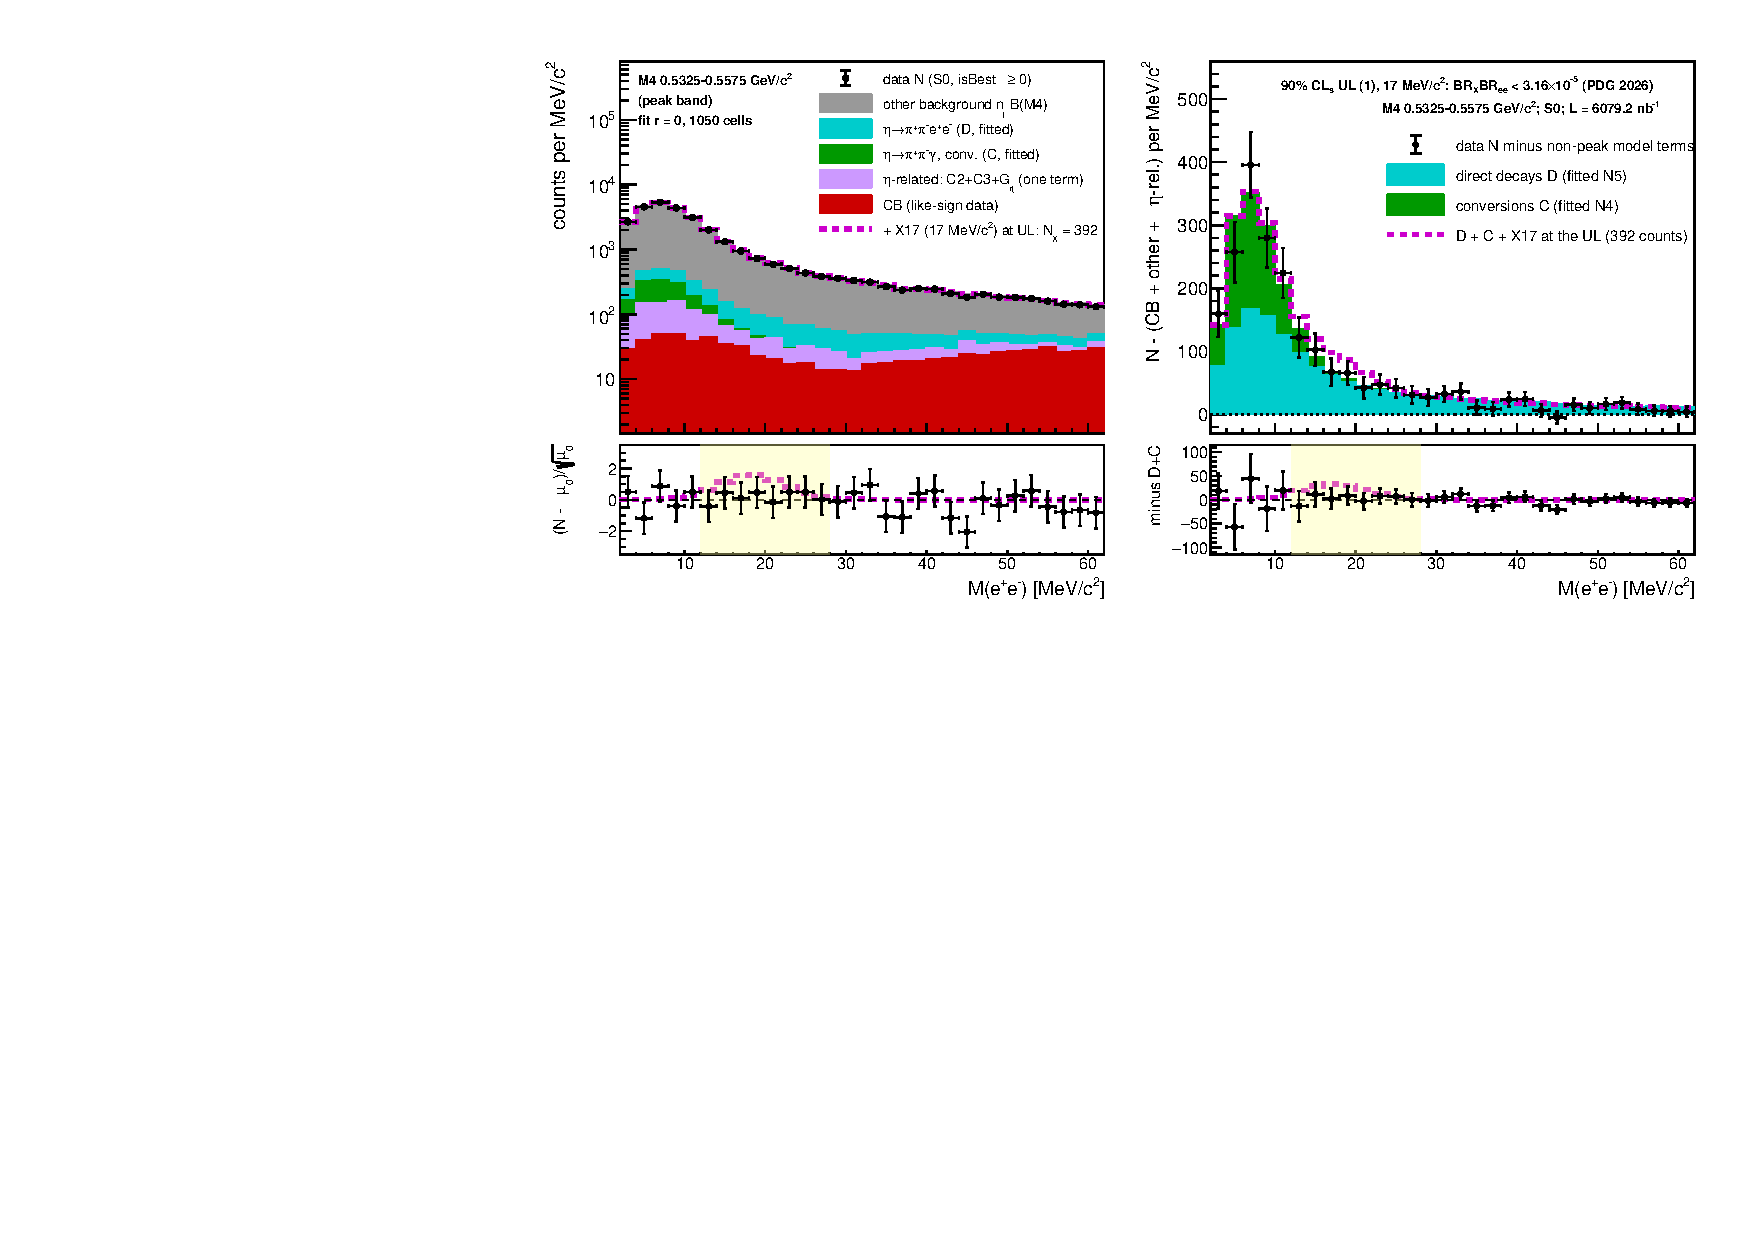
\includegraphics[width=0.90\textwidth]{figs_all/fix_X1_pdg26_cnt.pdf}
\caption{\textbf{What it shows: the \Mee spectrum of the $\eta$ peak is described without X17.}
An X17 at the upper limit (dotted magenta) would raise it above the data near 17\,\MeVcc.
Selection: data S0 (PT3 trigger, event vertex at $\vz>-160$\,mm, \betanew identification (pions $3\sigma$, leptons $5\sigma$ with a RICH ring), corrected momenta, all stored combinations (isBest $\ge0$), both pions in the event-vertex fit); peak band \Mfour 0.5325--0.5575\,\GeVcc, \Mee 2--62\,\MeVcc in 2\,\MeVcc bins; the model fitted with $r=0$ in \Mfour 0.5225--0.6100\,\GeVcc $\times$ \Mee 2--62\,\MeVcc; CB from the like-sign data; SMASH with the same cuts.
\Mee of the $\eta$ peak band (\Mfour 0.5325--0.5575\,\GeVcc), counts per \MeVcc, data S0.
Left (log scale): data $N$ (black) and the frozen 2D model fitted with $r=0$: CB from like-sign data (red), the $\eta$-related term
C2+C3+\Geta (violet), conversions $\eta\to\pipi\gamma$ (C4, green), direct decays $\eta\to\ppee$ (C5, cyan), other background (grey); lower
pad $(N-\mu_0)/\sqrt{\mu_0}$; yellow band: the \Mee range 12--28\,\MeVcc, blinded until the freeze. Right: the same after subtracting the
non-peak terms, with the fitted direct decays and conversions and with these plus the X17 line at the limit (392 counts); lower pad: the
residual after the direct decays and conversions. Same figure as Fig.~\ref{fig:X1}.}
\label{fig:res-x17spec}
\end{figure}

\begin{figure}[tbp]
\centering
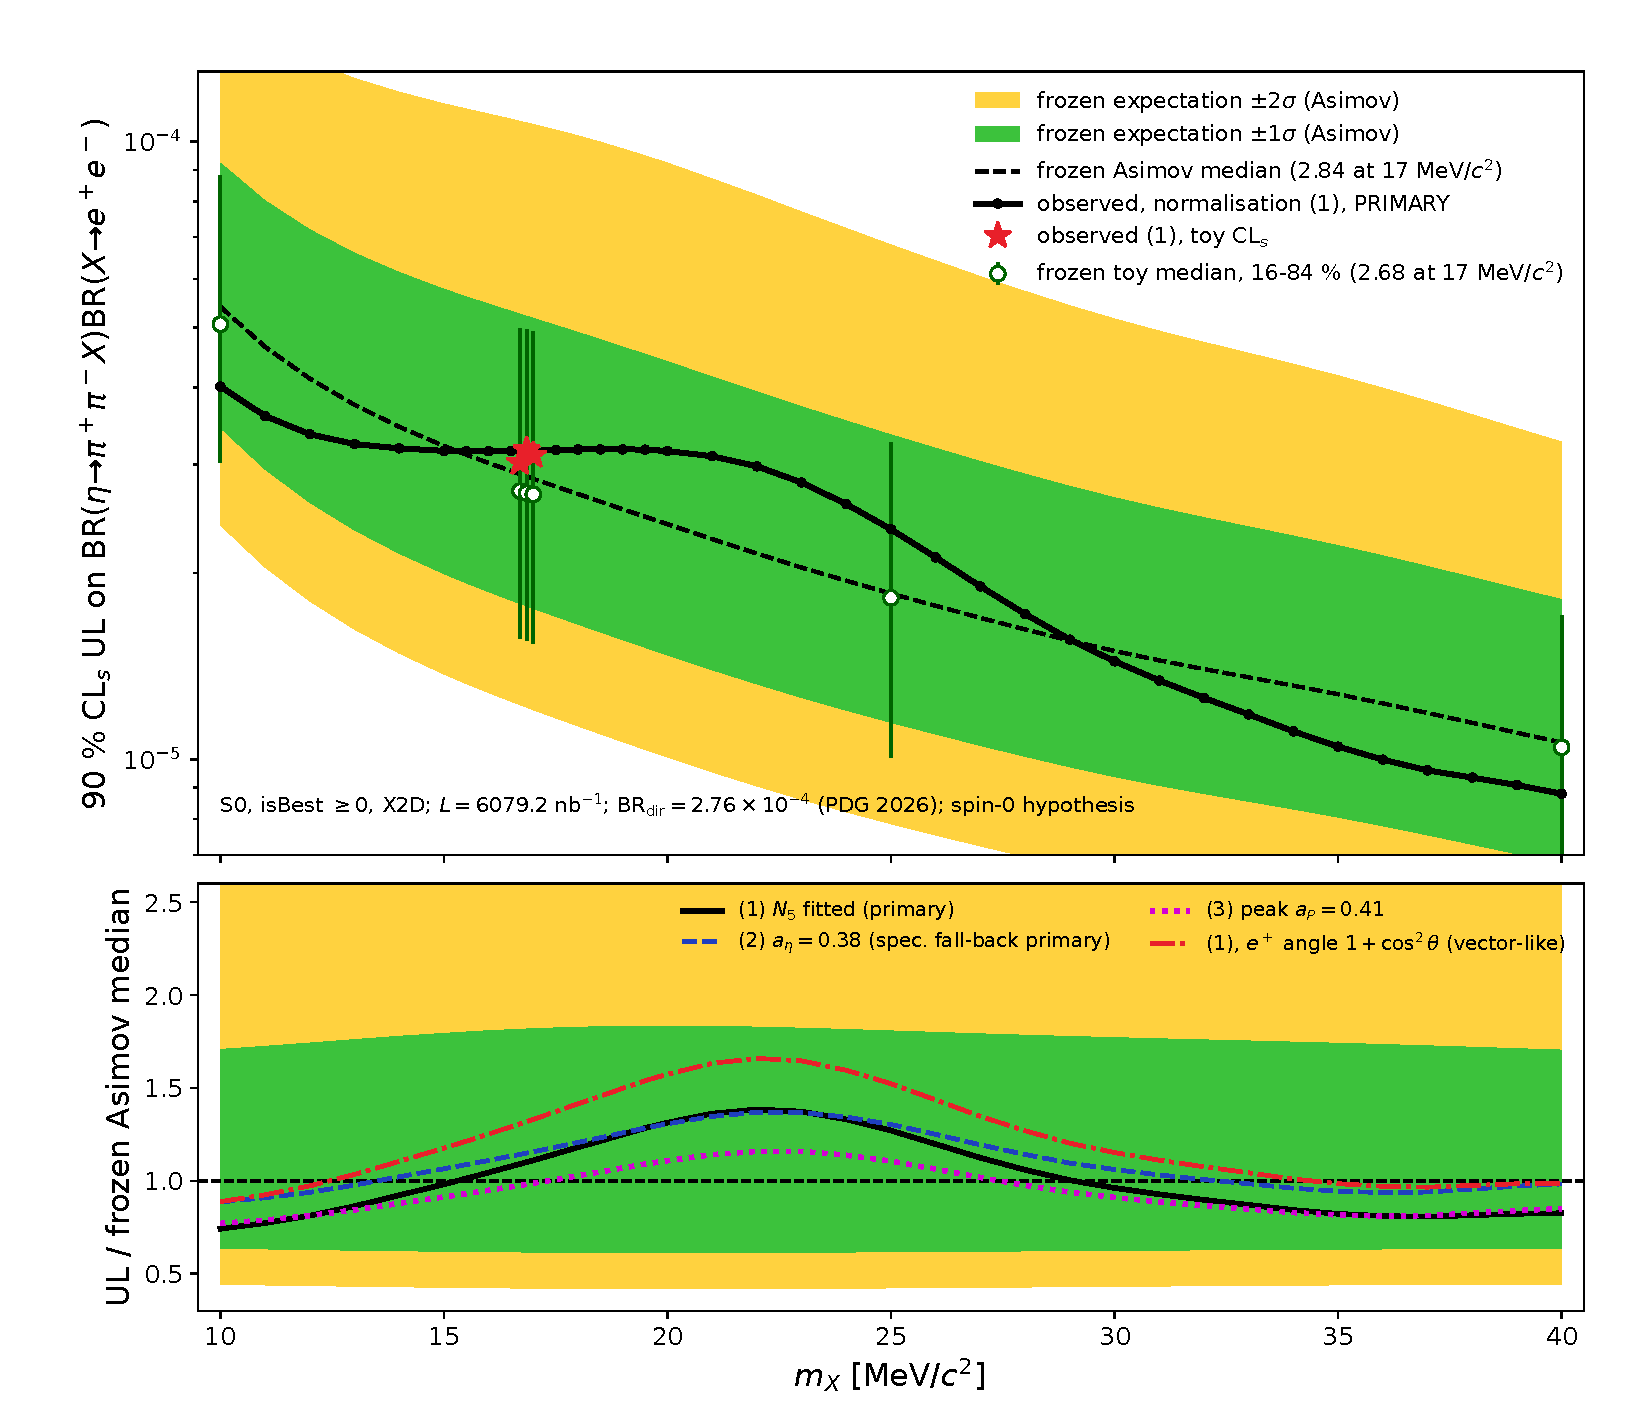
\includegraphics[width=0.75\textwidth]{figs_all/fix_X2_pdg26.pdf}
\caption{\textbf{What it shows: the observed limit stays inside the band expected without a signal.}
The observed limit (black) stays inside the $\pm1\sigma$ band expected without a signal at every mass, so no X17 is seen.
Selection: data S0 (PT3 trigger, event vertex at $\vz>-160$\,mm, \betanew identification (pions $3\sigma$, leptons $5\sigma$ with a RICH ring), corrected momenta, all stored combinations (isBest $\ge0$), both pions in the event-vertex fit); the plane \Mfour 0.5225--0.6100\,\GeVcc $\times$ \Mee 2--62\,\MeVcc; CB from the like-sign data; SMASH with the same cuts; the expected limits frozen on the \Mee side bands 2--12 and 28--62\,\MeVcc.
X17: 90\,\% CL$_s$ upper limit on \BRX against the X17 mass (spin-0), with the PDG 2026 BR$(\eta\to\ppee)=2.76\times10^{-4}$ (D25). Black: observed. Dashed line with green and yellow bands: the
limit expected without a signal ($\pm1\sigma$, $\pm2\sigma$), fixed before the unblinding; open circles: the same from pseudo-experiments. Bottom:
the variants divided by the expected median. Same figure as Fig.~\ref{fig:X2}.}
\label{fig:res-x17}
\end{figure}

%----------------------------------------------------------------------
\subsection{SMASH does not describe the shape of the spectrum}
\label{sec:res-before}
With every channel at its own SMASH cross section $\times$ PDG branching ratio and nothing adjusted, data/SMASH is 0.86 in the bump window,
1.10 in the peak window, 1.27 just above the peak (0.565--0.70\,\GeVcc) and 0.74 at 0.90--1.10\,\GeVcc; one common scale leaves
$\chi^2/\mathrm{ndf}=12$. SMASH does not describe the shape of the spectrum (Fig.~\ref{fig:res-before}). Part of the excess above the peak is target material: about
13--15\,\% of the data ($N-\mathrm{CB}$, all counts including the $\eta$) in 0.40--0.70\,\GeVcc comes from the target walls, which SMASH does not
simulate (Fig.~\ref{fig:res-walls}). Above the \piz mass the
data have 1.5--2 times more \ee pairs than SMASH, and only about 0.3 of its K$^0_S$ (the event-vertex cut explains at most a factor 1.4 of this).
After the non-$\eta$ background is normalised to the data above the peak (Fig.~\ref{fig:res-after}; in the class \Mee$\ge10$\,\MeVcc the ratio
there goes from 1.20 to 1.00 by construction), the SMASH $\eta$ peak and bump stand out as too high, the data want about 0.4 of them; below the
bump (0.400--0.455\,\GeVcc) the ratio is 0.83 (most bins 0.75--0.85): the background carried down from above the peak overshoots
the data there.
\textbf{Status:} measured (a direct comparison; the 6.9\,\% uncertainty of the luminosity is common to all ratios). \textbf{Details:}
\S\ref{sec:before}, \S\ref{sec:norm}, \S\ref{sec:cr}.

\begin{figure}[!tbp]
\centering
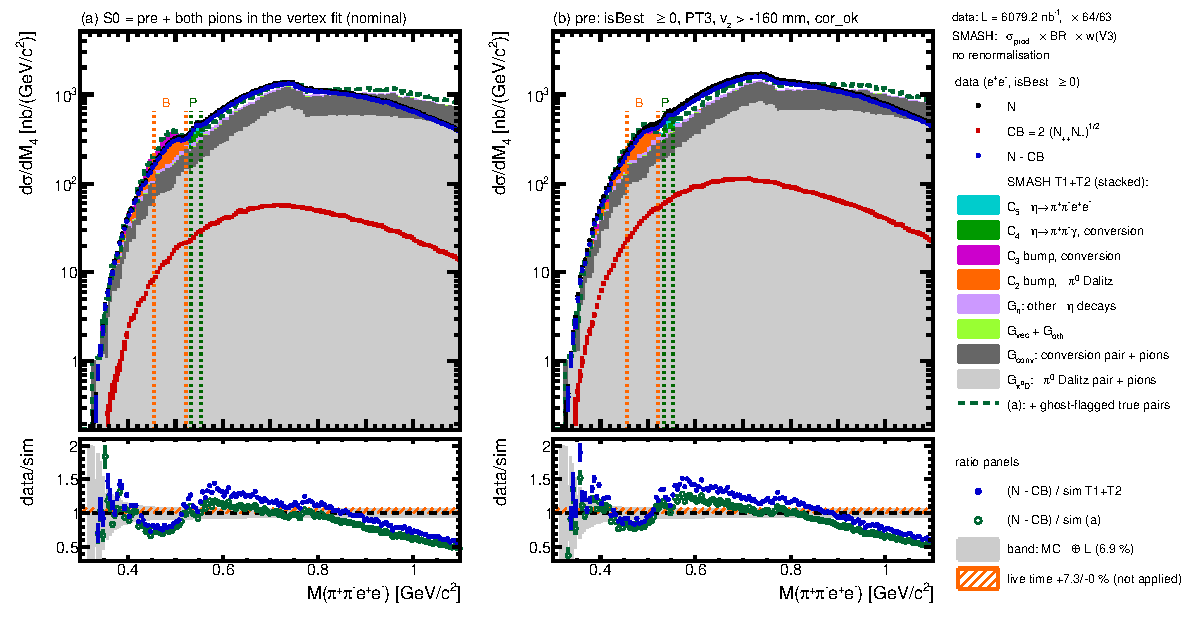
\includegraphics[width=0.88\textwidth]{figs_all/fix_B1.pdf}
\caption{\textbf{What it shows: with nothing adjusted, SMASH does not describe the spectrum shape.}
SMASH (stacked colours) lies below the data just above the $\eta$ peak and above them at large \Mfour (data/SMASH from 1.27 to 0.74).
Selection: (a) data S0 (PT3 trigger, event vertex at $\vz>-160$\,mm, \betanew identification (pions $3\sigma$, leptons $5\sigma$ with a RICH ring), corrected momenta, all stored combinations (isBest $\ge0$), both pions in the event-vertex fit); (b) ``pre'' (the same without the pion-vertex condition); all \Mpipi and \Mee; CB $=2\sqrt{N_{++}N_{--}}$ (10\,\MeVcc cells, $k=1$); SMASH $T_1+T_2$ with the same cuts, nothing renormalised.
\Mfour from 0.30 to 1.10\,\GeVcc (log
scale) before any renormalisation: (a) S0 (nominal), (b) ``pre''. Data (isBest $\ge0$): $N$ black, CB $=2\sqrt{N_{++}N_{--}}$ from the
like-sign data red, $N-\mathrm{CB}$ blue, as $d\sigma/dM_4$ ($\times64/63$, $L=6079.2\,\nbinv$). Stacked: SMASH $T_1+T_2$ by group at
$\sigma_{\mathrm{prod}}\times$PDG BR$\times$V3; dashed: ghost variant (a). Dotted: windows B and P. Lower panels: $(N-\mathrm{CB})$/simulation
(full) and /variant (a) (open); grey band: MC $\oplus$ 6.9\,\% luminosity; hatched: possible live-time correction $+7.3/-0$\,\% (not
applied). Same figure as Fig.~\ref{fig:B1}.}
\label{fig:res-before}
\end{figure}

\begin{figure}[!tbp]
\centering
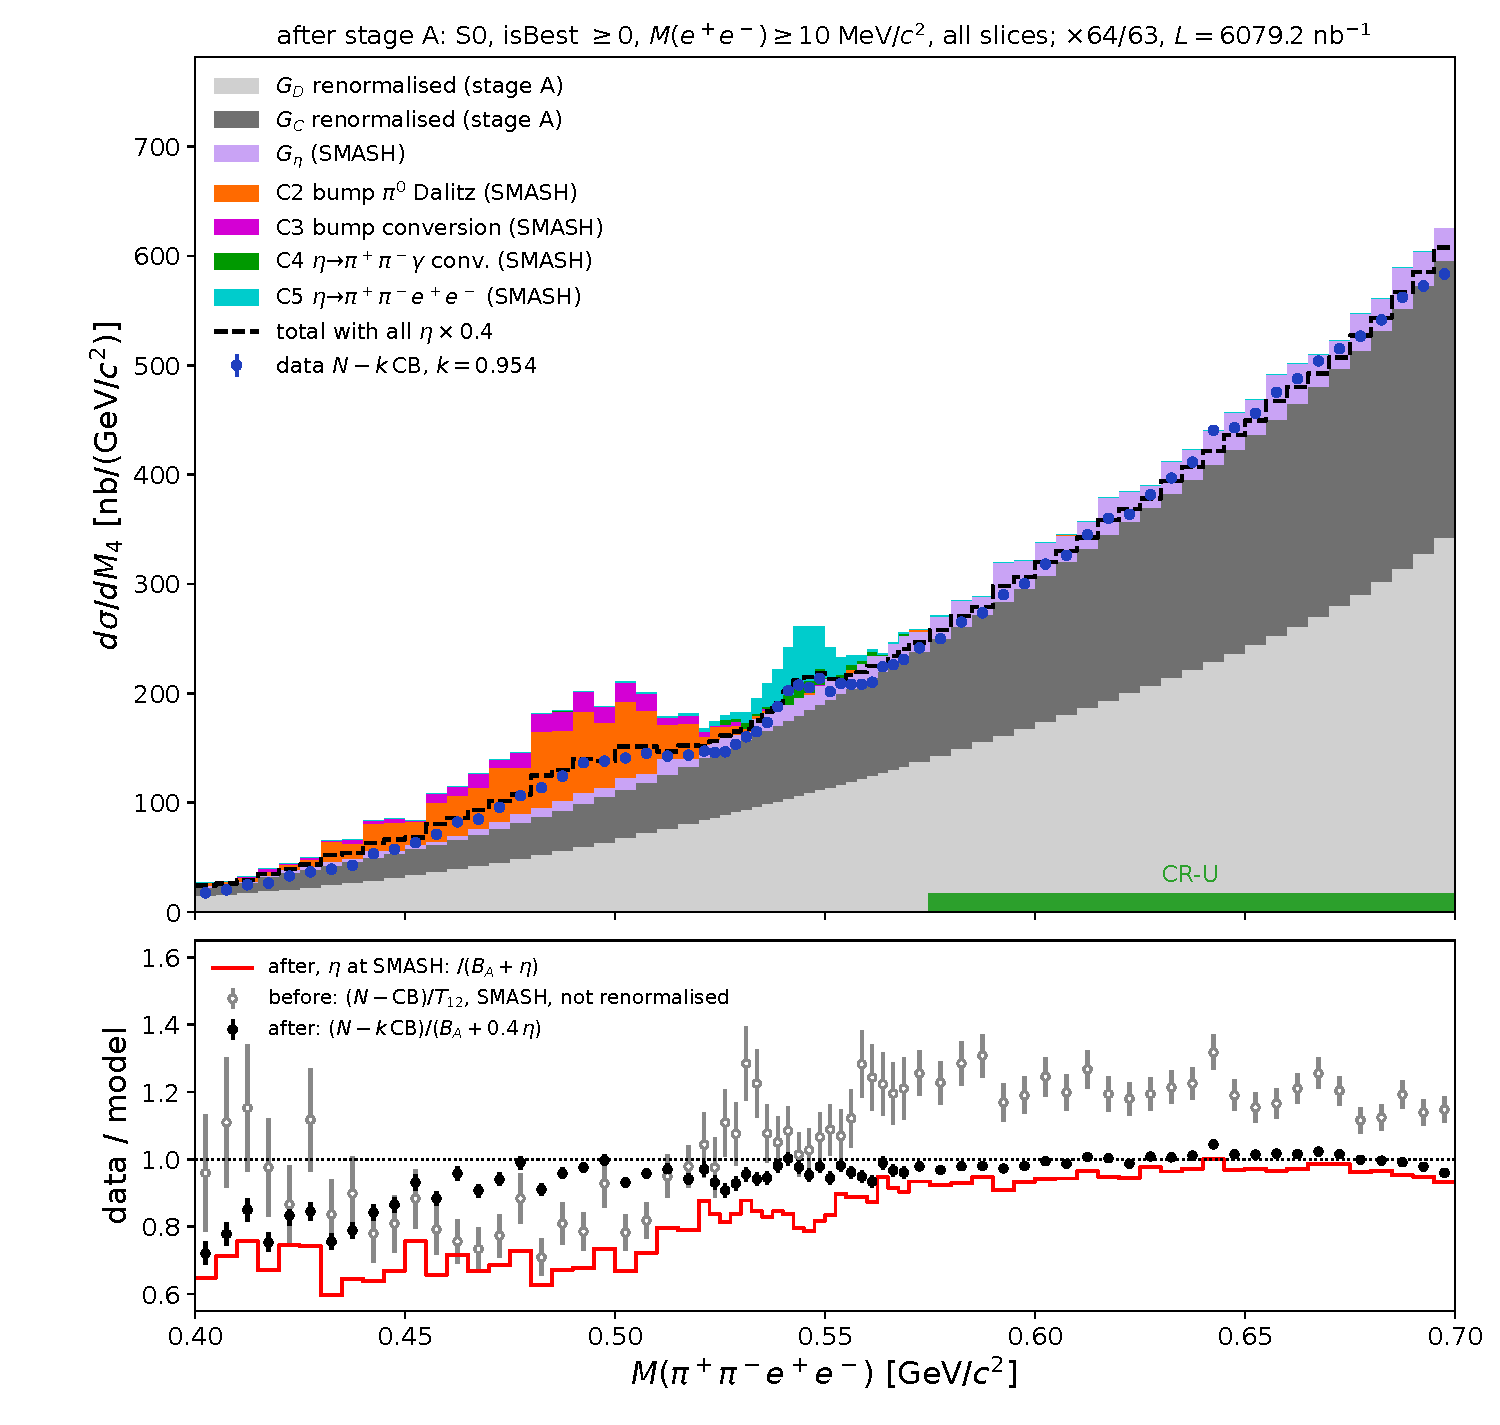
\includegraphics[width=0.58\textwidth]{figs_all/fix_C3.pdf}
\caption{\textbf{What it shows: with the background normalised, the SMASH $\eta$ peak and bump are too high.}
Once the non-$\eta$ background is normalised above the peak, the SMASH $\eta$ peak and bump are clearly too high; the data want about 0.4
of them.
Selection: data S0 (PT3 trigger, event vertex at $\vz>-160$\,mm, \betanew identification (pions $3\sigma$, leptons $5\sigma$ with a RICH ring), corrected momenta, all stored combinations (isBest $\ge0$), both pions in the event-vertex fit); \Mee$\ge10$\,\MeVcc; the five \Mpipi slices summed; CB $\times k=0.954$; the SMASH non-$\eta$ background (same cuts) renormalised in \Mfour 0.575--0.700\,\GeVcc with \Mee$\ge10$\,\MeVcc.
SMASH against the data, after normalising the non-$\eta$ background above the peak. Data
$N-k\,\mathrm{CB}$ (blue points, $M(e^+e^-)\ge10$\,\MeVcc, all \Mpipi slices) against the stacked SMASH model: the non-$\eta$ background
(grey) is scaled to the data in 0.575--0.70\,\GeVcc (green bar), all $\eta$ channels are shown at the SMASH prediction (bump orange/magenta,
peak green/cyan, other $\eta$ decays violet), and the dashed line is the total with every $\eta$ channel scaled by 0.4. Lower panel:
data/model before (grey, SMASH as it is) and after (black) the normalisation. Above the peak the normalised model matches the data (ratio
1.0, was 1.2); below the bump the background carried down from above the peak overshoots the data (ratio 0.83 over 0.400--0.455\,\GeVcc,
most bins 0.75--0.85), which is why the background-subtracted bump area (B4) is not determined. Same figure as Fig.~\ref{fig:C3}.}
\label{fig:res-after}
\end{figure}

%----------------------------------------------------------------------
\subsection{A flexible SMASH description: one \texorpdfstring{$\eta$}{eta} scale, a background above SMASH, an incomplete model}
\label{sec:res-flex}
\begin{figure}[!t]
\centering
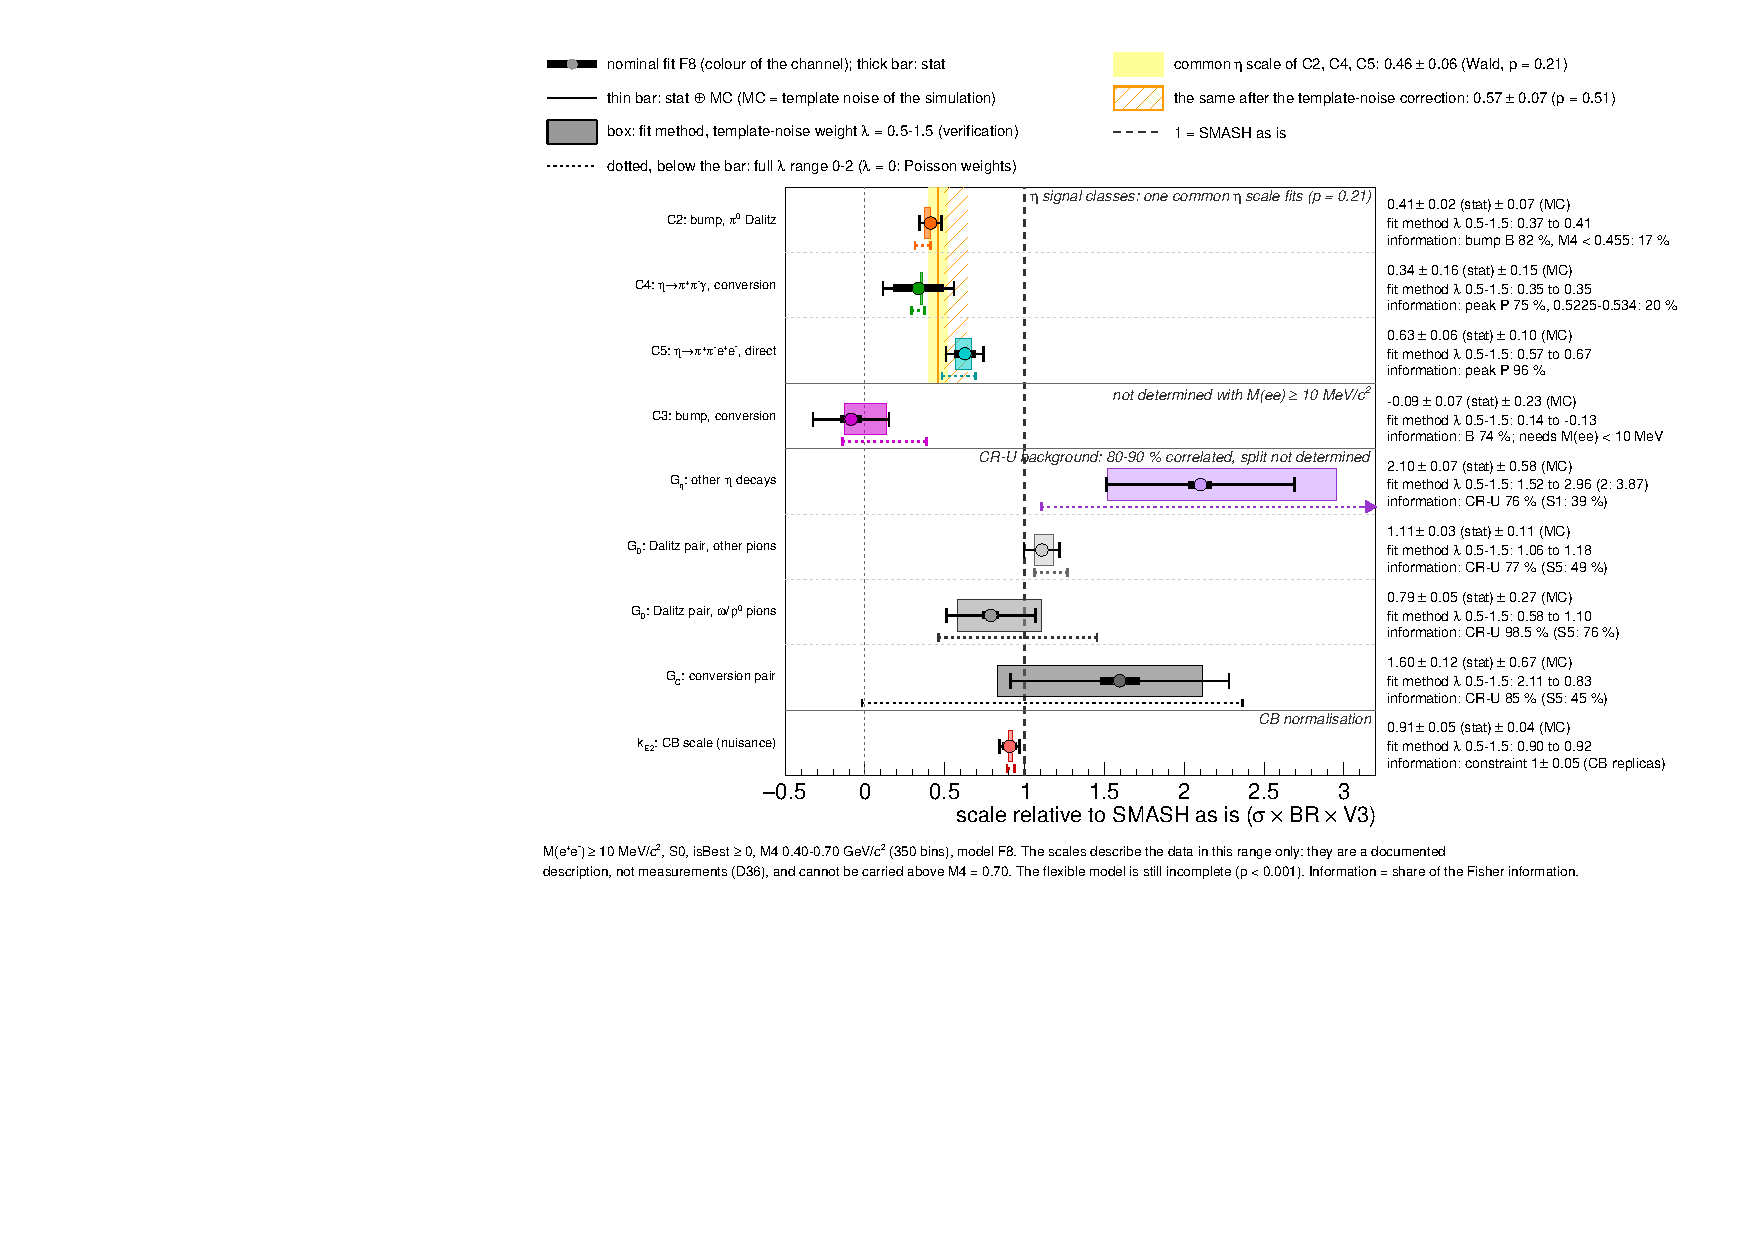
\includegraphics[width=0.97\textwidth]{figs_all/flex_scales_v2.pdf}
\caption{\textbf{What it shows: with a free scale per SMASH channel, the $\eta$ signal classes C2, C4 and C5 share one scale of about 0.46 of
SMASH; the background scales above the peak are large, correlated and depend on the fit method; C3 is not determined.}
Selection: data S0 (PT3 trigger, event vertex at $\vz>-160$\,mm, \betanew identification (pions $3\sigma$, leptons $5\sigma$ with a RICH ring), corrected momenta, all stored combinations (isBest $\ge0$), both pions in the event-vertex fit); \Mee$\ge10$\,\MeVcc; five \Mpipi slices (below 0.34, 0.34--0.37, 0.37--0.39, 0.39--0.43, from 0.43\,\GeVcc); \Mfour 0.40--0.70\,\GeVcc; CB $\times$ \kEtwo (within $1\pm0.05$); SMASH with the same cuts.
Nominal flexible fit F8: S0, isBest $\ge0$, \Mee$\ge10$\,\MeVcc, \Mfour 0.40--0.70\,\GeVcc, five \Mpipi slices (350 bins). Every scale against 1
(SMASH as is, dotted line), in the colour of its channel (C2 orange, C3 magenta, C4 green, C5 cyan, \Geta violet, $G_D$ and $G_C$ greys, \kEtwo red).
Thick bar: stat; thin bar: stat $\oplus$ MC (the template noise of the simulation). Shaded box: the spread with the fit method (weight
$\lambda=0.5$--1.5 of the template noise in the fit weights, from the verification); dotted line below each bar: the full range $\lambda=0$--2
(arrow: \Geta reaches 3.87 at $\lambda=2$). Yellow band: the common $\eta$ scale of C2, C4, C5, $0.46\pm0.06$ ($p=0.21$); hatched: $0.57\pm0.07$
after the template-noise correction ($p=0.51$). Rows: $\eta$ signal classes; C3, not determined with \Mee$\ge10$\,\MeVcc; the background above
the peak (CR-U, 0.565--0.70\,\GeVcc), 80--90\,\% correlated, its split not determined; the CB scale \kEtwo. Right: value $\pm$ stat $\pm$ MC, the
$\lambda$ range, and what fixes the scale (share of the Fisher information by \Mfour region and slice). The scales describe the data in this
range only; they are not measurements (D36), cannot be carried above \Mfour$=0.70$\,\GeVcc, and the model is incomplete ($p<0.001$).}
\label{fig:res-flex}
\end{figure}

\textbf{What was done.} SMASH is not taken as exact. Every SMASH component got its own free scale (1 $=$ SMASH as is): the bump classes C2 and
C3, the peak classes C4 and C5, the other $\eta$ decays \Geta, the non-$\eta$ Dalitz pairs $G_D$ (split into pairs whose pions come from an $\omega$
or $\rho^0$ and the rest) and the non-$\eta$ conversion pairs $G_C$. The 350 bins of Part~III (\Mee$\ge10$\,\MeVcc) were fitted with the Part~III
method, which reproduces the Part~III template fit F-main to $4\times10^{-8}$. Every scale is documented with what fixes it: C2 by the bump window
(82\,\% of its information), C5 by the peak window (96\,\%), C4 by the peak window (75\,\%), and \Geta, both parts of $G_D$ and $G_C$ all by the
same bins above the peak (76--98\,\%). The nominal model (F8) was chosen with three conditions added after the first result of the model ladder
had been seen (D36).

\textbf{What the data say} (Fig.~\ref{fig:res-flex}; the fit itself in Fig.~\ref{fig:res-flexfit}):
\begin{itemize}\setlength{\itemsep}{1pt}
\item \textbf{One $\eta$ scale for the $\eta$ signal classes.} The bump (C2, 0.41), the converted photons of the peak (C4, 0.34) and the direct decays
      (C5, 0.63) are consistent with one common scale, $0.46\pm0.06$ of SMASH ($p=0.21$), or $0.57\pm0.07$ after correcting the attenuation that
      the noisy simulated templates are known to cause ($p=0.51$). This agrees with the peak (0.42) and the bump edge (0.39--0.43).
\item \textbf{The direct decays:} $s_{\mathrm{C5}}=0.63\pm0.12$ (stat $\oplus$ MC) with about $\pm0.1$ from the model and the fit method (0.44--0.94 over
      the variants); it is the most stable $\eta$ scale. The ratio C5/C2 agrees with the PDG branching ratios within 1--2$\sigma$ (1.5 $\pm$ 0.5).
\item \textbf{The non-$\eta$ background above the peak} (0.565--0.70\,\GeVcc) is 10--30\,\% above SMASH. How the excess splits between $G_D$, $G_C$
      and \Geta is \emph{not} determined: the three are fixed by the same bins and are 80--90\,\% correlated.
\item \textbf{The bump conversions C3} cannot be fixed with \Mee$\ge10$\,\MeVcc ($-0.09\pm0.24$). With the class \Mee$<10$\,\MeVcc added, the
      conversion classes C3 and C4 come out at 0.32--0.34, conditional on an extra CB-like term for that class (its CB is not understood).
\end{itemize}

\textbf{What limits it} (the doubts, next to the evidence):
\begin{itemize}\setlength{\itemsep}{1pt}
\item \textbf{The model is still incomplete.} Hybrid GLS $\chi^2=604$ for 342 degrees of freedom, against $356\pm33$ for pseudo-data from a perfect
      model with the real template noise; none of 2000 reaches the data (largest 461): $p<0.001$. The fitted model lies 2\,\% above the data in
      total (5.8\,\% in the peak window, 10\,\% below 0.455\,\GeVcc), where pseudo-data give $-0.7\pm0.3$\,\%; the misfit sits at the low-mass edge of
      S2/S3 and in $\pm10$\,\% waves (Fig.~\ref{fig:res-flexfit}).
\item \textbf{The scales depend on the fit method far beyond their errors.} Giving the template noise less or more weight in the fit moves the
      correlated background scales along their degenerate direction (\Geta 1.1--3.9, $G_C$ 2.4--0, $G_D(\omega/\rho)$ 0.46--1.45) and the signal
      scales less (C2 0.31--0.41, C5 0.48--0.69). The nominal \Geta $=2.10$, $G_C=1.60$ and $G_D(\omega/\rho)=0.79$ are therefore not determinations.
\item \textbf{The template noise of the simulation dominates}: the MC error is 1--8 times the statistical one, and in the pseudo-data test it
      biases C2 by $-20$\,\% and C4 by $-58$\,\%; only C5, $G_C$ and \kEtwo pass that test as specified.
\item \textbf{The model choice is a convention.} The fit's $\chi^2$ (hybrid GLS) grows and falls with the fitted scales, so a model with fewer free
      scales can get a lower value (all five $\eta$ scales tied: 574 instead of 604): it cannot rank nested models, and the ladder that chose F8 is
      not a significance test.
\item \textbf{Above \Mfour$=0.70$\,\GeVcc the scaled components fail} (CB scale 7--8$\sigma$ from its constraint, an unphysical negative $G_C$):
      the scales must not be carried above 0.70.
\end{itemize}
\textbf{Status:} a documented description of the data with SMASH (D36), not a measurement; no headline number is taken from it.
\textbf{Details:} \S\ref{sec:flex}.

\begin{figure}[!tbp]
\centering
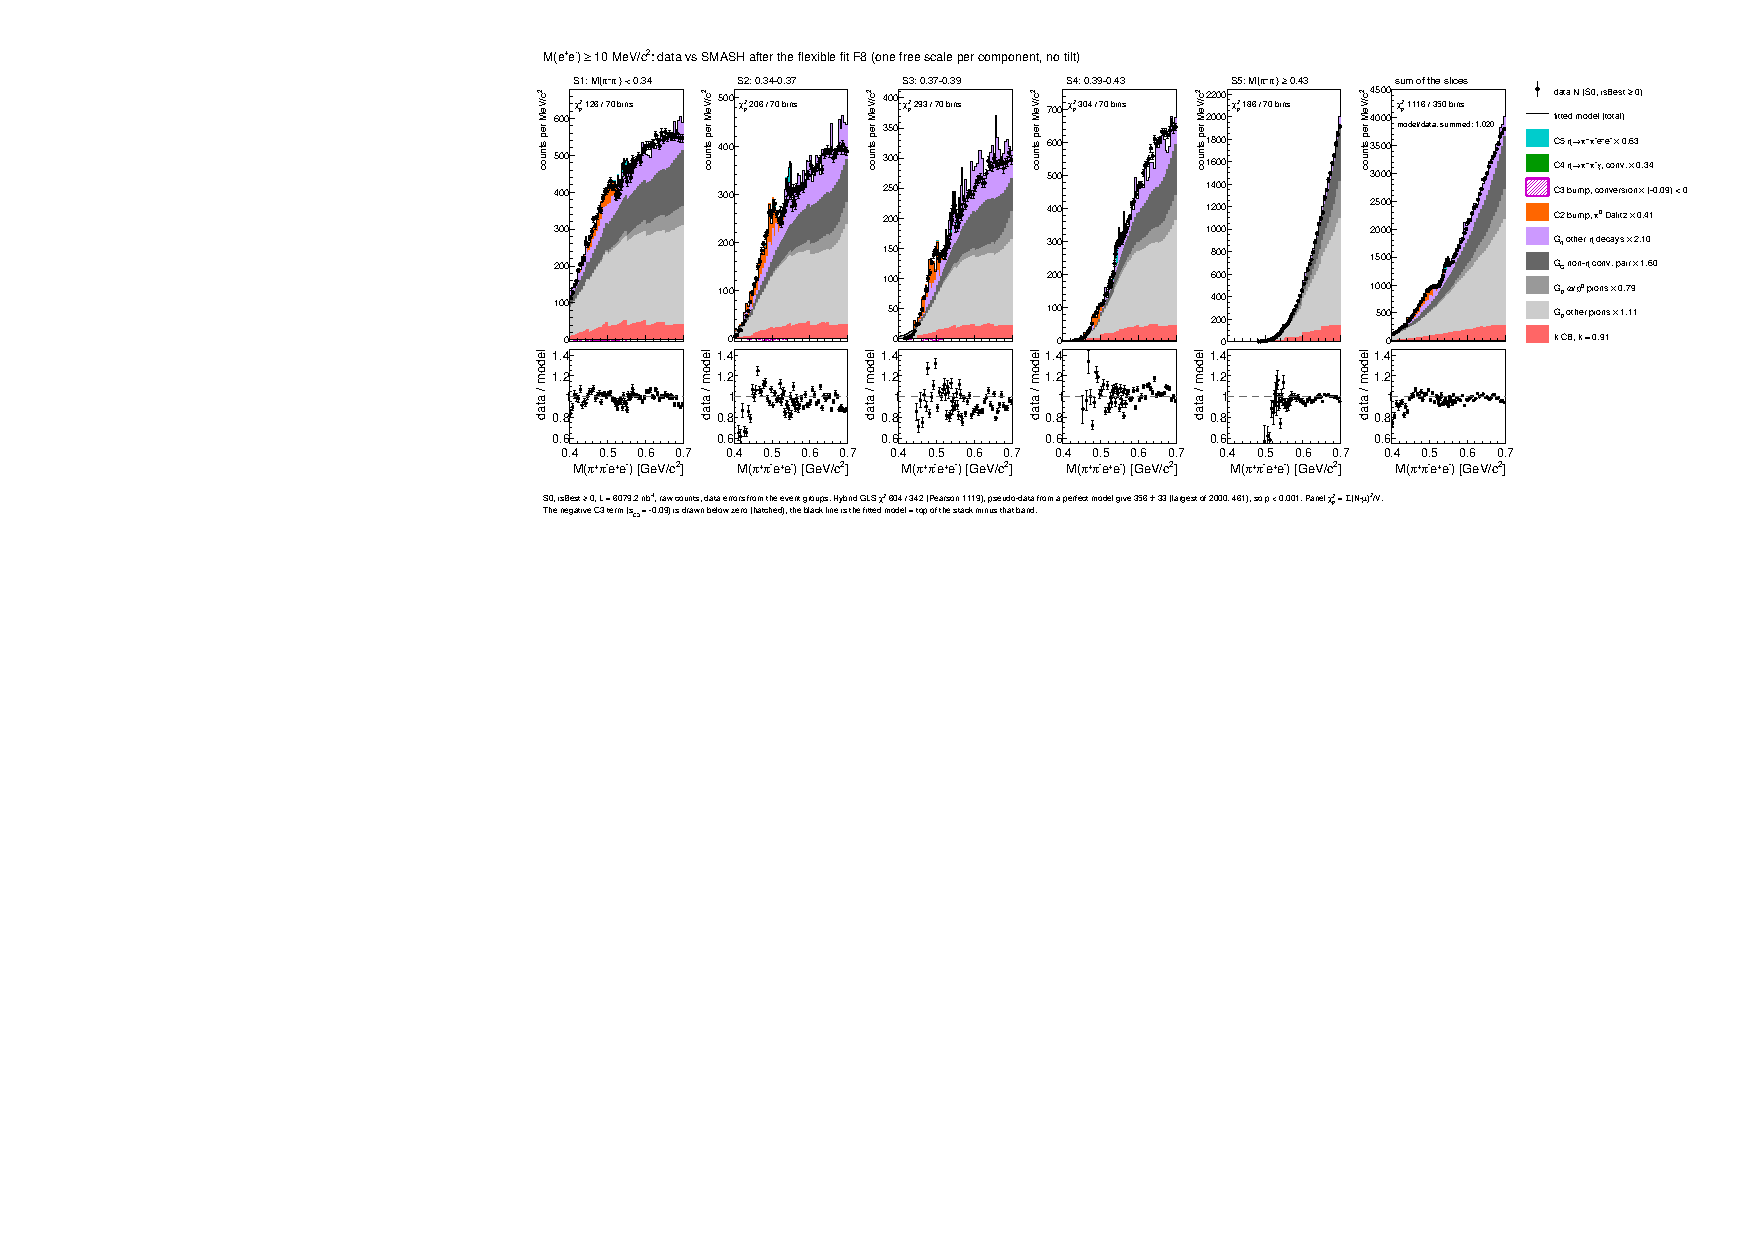
\includegraphics[width=\textwidth]{figs_all/flex_spectra_fit_v2_cnt.pdf}
\caption{\textbf{What it shows: after the flexible fit the model follows the data within about $\pm10$\,\% in most bins, but it lies 2\,\% above them
in total and misses the low-mass edge of S2 and S3.}
Selection: data S0 (PT3 trigger, event vertex at $\vz>-160$\,mm, \betanew identification (pions $3\sigma$, leptons $5\sigma$ with a RICH ring), corrected momenta, all stored combinations (isBest $\ge0$), both pions in the event-vertex fit); \Mee$\ge10$\,\MeVcc; five \Mpipi slices (below 0.34, 0.34--0.37, 0.37--0.39, 0.39--0.43, from 0.43\,\GeVcc); \Mfour 0.40--0.70\,\GeVcc; CB $\times$ \kEtwo (within $1\pm0.05$); SMASH with the same cuts.
Data $N$ (black points; event-group errors), S0, isBest $\ge0$, $L=6079.2\,\nbinv$, raw counts per \MeVcc, \Mee$\ge10$\,\MeVcc, in the five
\Mpipi slices S1--S5 and summed (right). Stack, each component times its fitted scale (legend): $k\,$CB (red, $k=0.91$), $G_D$ other pions
(light grey) and $\omega/\rho^0$ pions (mid grey), $G_C$ (dark grey), \Geta (violet), C2 (orange), C4 (green), C5 (cyan). The negative C3 term
($s_{\mathrm{C3}}=-0.09$) is drawn as a hatched band below zero; the black line is the fitted model (top of the stack minus that band). Lower row:
data/model. Panel $\chi^2_P=\sum(N-\mu)^2/V$ with the fit variance $V$ (their sum, 1116, is the global Pearson value 1119 without the \kEtwo
constraint term). Hybrid GLS $\chi^2=604/342$; pseudo-data from a perfect model give $356\pm33$ (largest of 2000: 461), so $p<0.001$. Summed
model/data: 1.020.}
\label{fig:res-flexfit}
\end{figure}

%----------------------------------------------------------------------
\subsection{After the typical \texorpdfstring{$\eta$}{eta} and X17 cuts of earlier analyses}
\label{sec:res-e1}
Earlier analyses of this channel select $\eta$-like combinations with three kinematic cuts: the angle between the \pipi and \ee systems below $50^\circ$
in the laboratory and above $140^\circ$ in the $\eta$ rest frame, and \Mpipi$<0.46$\,\GeVcc (0.42 in the old code), often with OA$>2^\circ$
(cut sets \cs{E1}--\cs{E4}). Their aim is to enhance a possible $\eta\to\pipi X17$ signal; OA$<6^\circ$ (\cs{X1}--\cs{X4}) was proposed because
X17 pairs are expected to be close. Part~III does not use these cuts (D3), but at the analyst's request the data are compared with SMASH after
them, on ``pre'' and on S0 (22 selections; Fig.~\ref{fig:res-e1}). \emph{SMASH as it is} still lies below the data just above the peak: data/SMASH
in 0.56--0.70\,\GeVcc is 1.23--1.45 on the ``pre'' base (1.354 after the cuts of the slides, \cs{E1}) and 1.16--1.34 on the S0 base, i.e.\ the data
exceed SMASH by 16--45\,\%. The $\chi^2/\mathrm{ndf}$ falls after the cuts only because counts are removed (``pre'' 79 $\to$ \cs{E1} 29); the mismatch per
bin does not (0.29 $\to$ 0.39). \emph{With scaled components} (every $\eta$ channel $\times0.40$, the non-$\eta$ background $\times c_b=1.25$--1.52
fitted above the peak) SMASH describes the S0-based selections about as well as S0 itself (mismatch 4--8\,\% per 5\,\MeVcc bin against 5\,\% for S0;
S0\,+\,\cs{X2old} 11\,\%) and the ``pre''-based ones less well (7--20\,\% against 6\,\% for ``pre''); a free $\eta$ scale gives 0.39--0.56 (0.399 on S0). The cuts do not enrich the $\eta$ (SMASH $\eta$ share of the peak window
0.298 $\to$ 0.308 after \cs{E1}): at a fixed \Mfour the $\eta$-rest angle cannot tell an $\eta$ from a background combination. A simulated X17 (17\,\MeVcc)
has OA$<6^\circ$ in two thirds of the cases (58\,\% in the X17 window), but so have the direct decays and the data of the same pair mass (57\,\%
and 50\,\%), and every cut acts on the X17 as on the direct decays within 5\,\%. In a simple count of the X17 window S0 alone is the most sensitive
of the 22 selections: on S0 the smallest X17 that a count could see grows by 2--12\,\% with the typical cuts and by 20--30\,\% with OA$<6^\circ$.
OA$<6^\circ$ raises the signal-to-background ratio by 19\,\% but keeps only 58\,\% of the X17, so it would help only if the background
systematics dominated.

\textbf{Drawn as in the earlier analysis} presented at HADES collaboration meetings (Fig.~\ref{fig:res-e1prev}), with SMASH scaled to the data
integral, SMASH gets the total right only by construction: it is about 20\,\% too high in the bump window (data/model 0.81) and about 10\,\% too
low just above the peak (1.09; $\chi^2/\mathrm{ndf}=5.8$ in 0.40--0.70\,\GeVcc), because one common factor hides the separate $\eta$ and
background levels. With our measured scales ($\eta$ about 0.42 of SMASH, non-$\eta$ background $\times1.42$) the same data are described up to
0.70\,\GeVcc ($\chi^2/\mathrm{ndf}=2.1$). The three-scale global fit of that approach gives $\eta$ scales of 0.45--0.74 of SMASH that move with the
treatment of the SMASH templates by 7--20 times their statistical errors, and the \Mee spectrum of the $\eta$-peak window minus the side bands
cannot test X17 (its residual changes sign within reasonable choices); both approaches agree only that SMASH's $\eta$ must come down and its
non-$\eta$ background go up by 25--45\,\%. The best combination only (isBest $=1$), shown only to reproduce the earlier approach, gives the same picture.

\textbf{Status:} comparison requested by the analyst, not used for any result (D3; D34 ruled by the analyst on 15 November 2026: the typical cuts are \emph{not} applied, because the numbers show they do not help; the variants with the cuts stay shown, with their numbers).
\textbf{Details:} \S\ref{sec:e1}; the earlier style in \S\ref{sec:e1prev}.

\begin{figure}[!tbp]
\centering
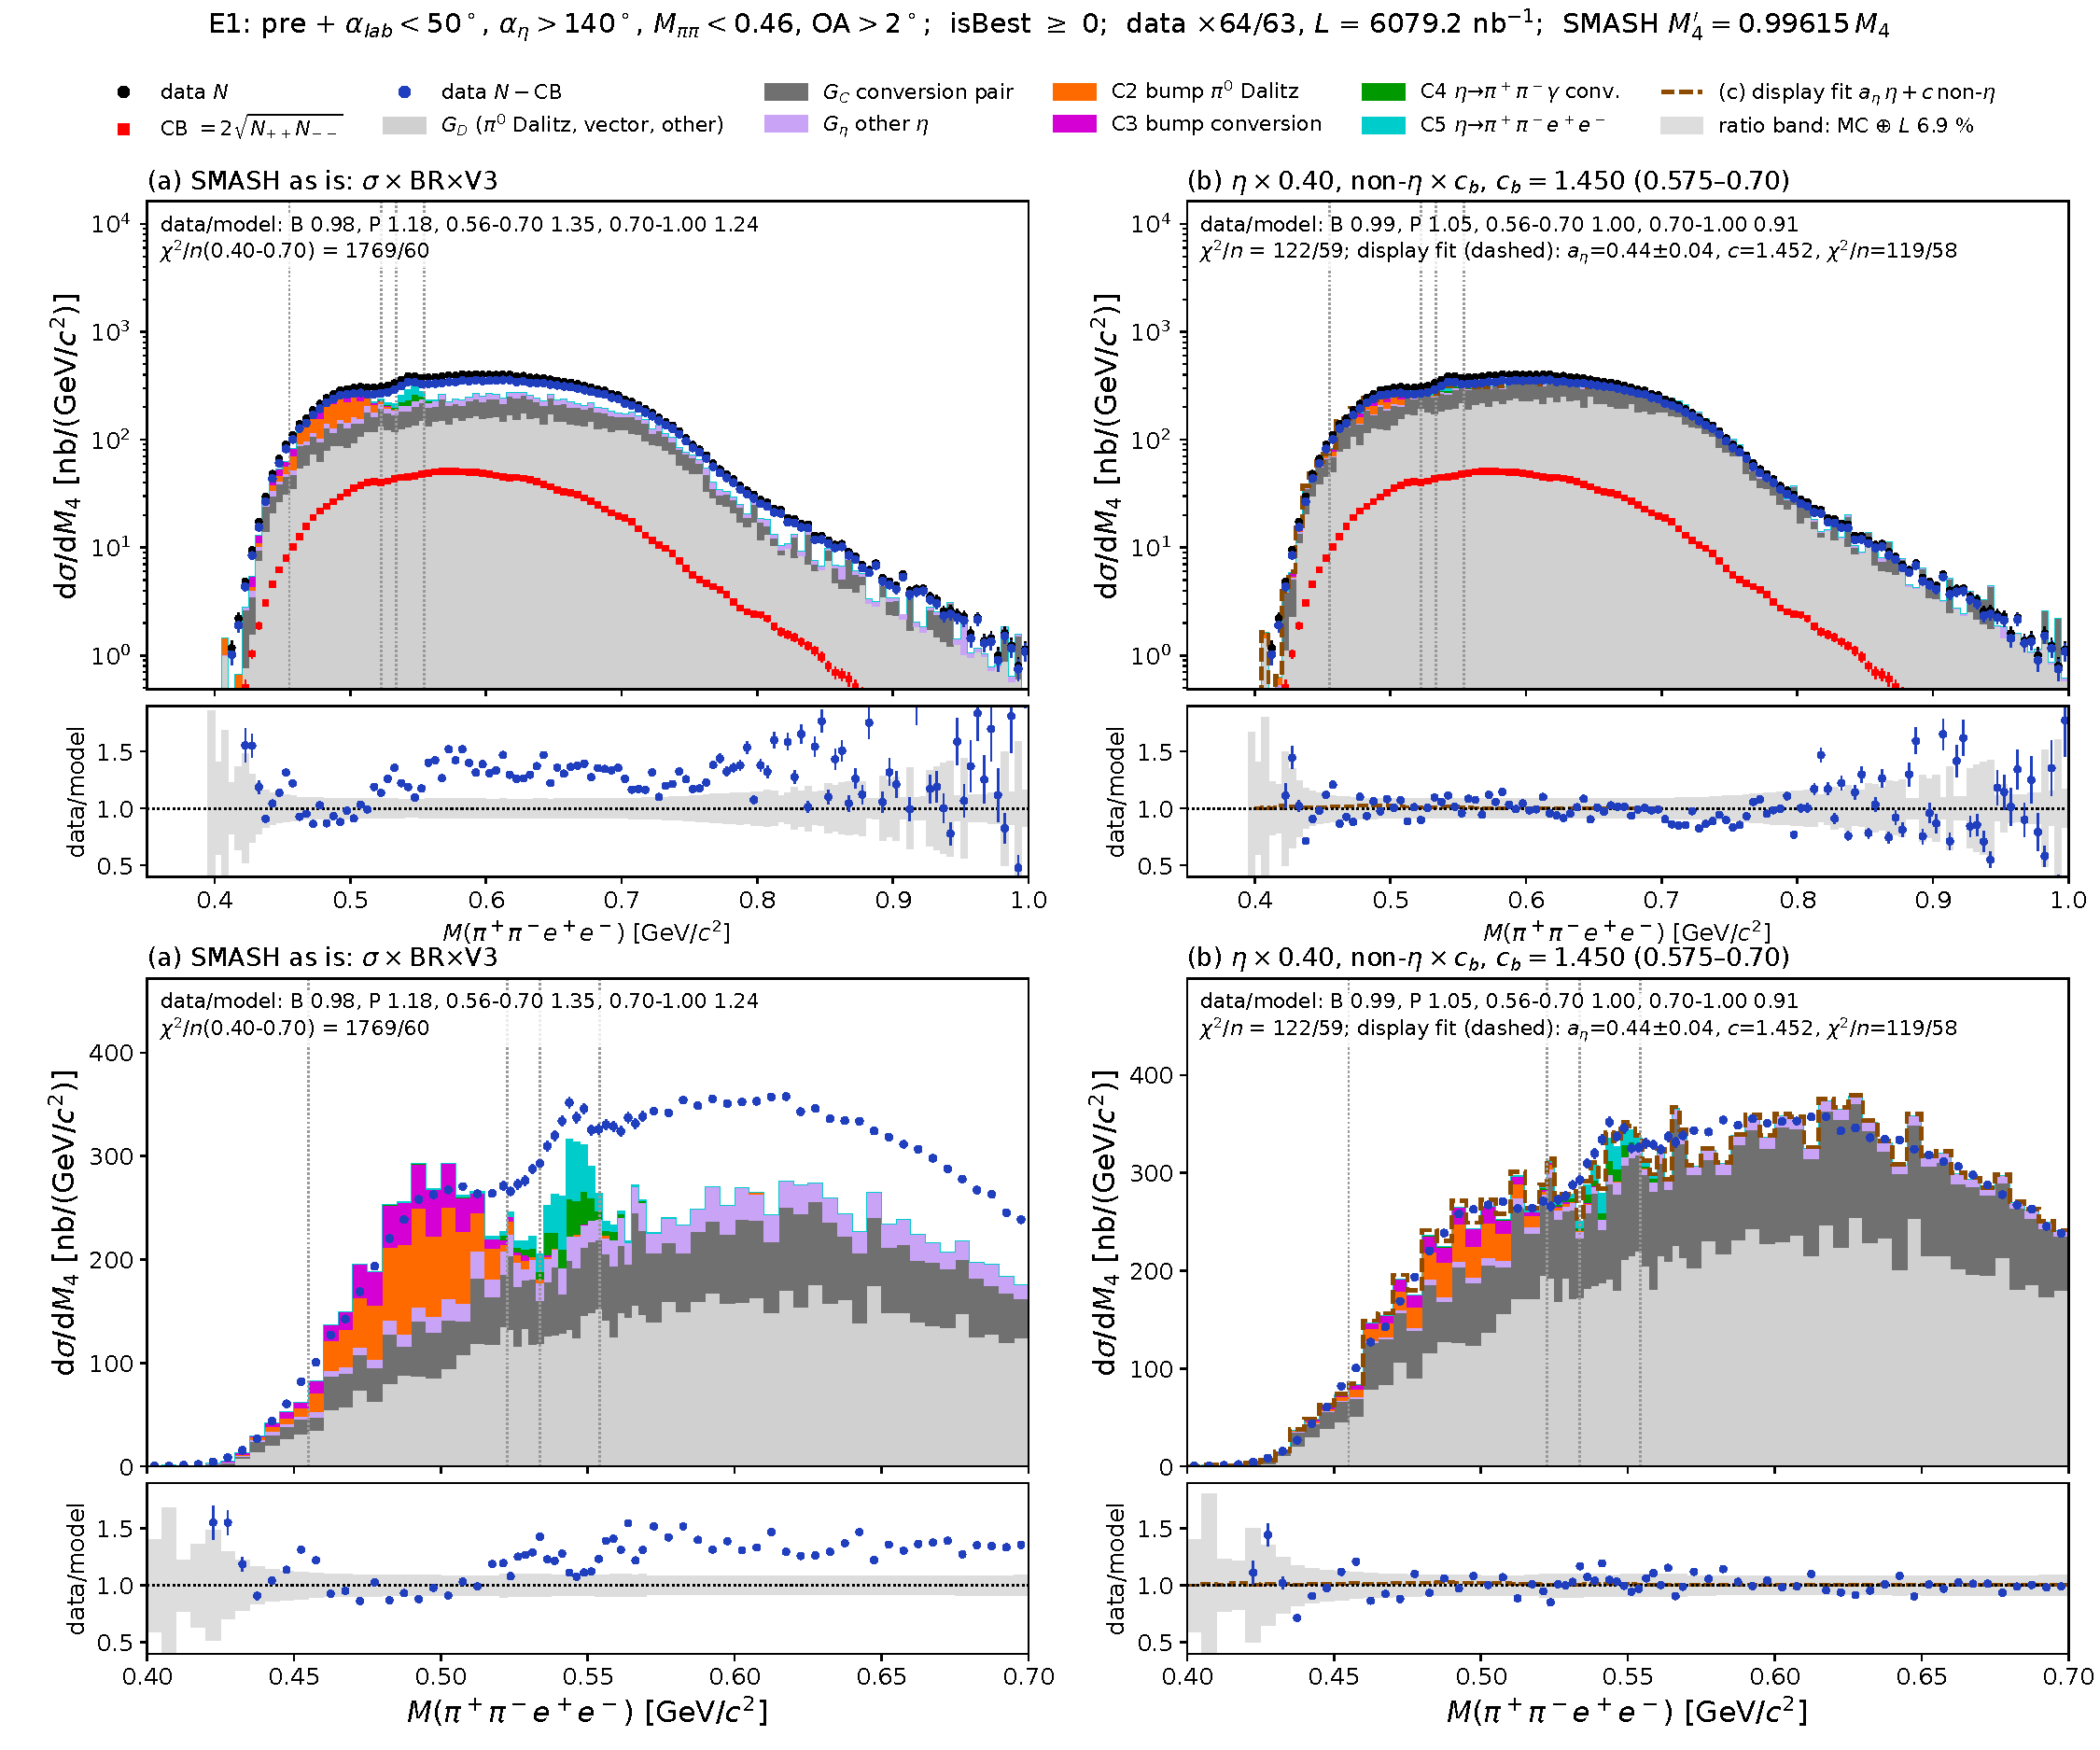
\includegraphics[width=0.90\textwidth]{figs_all/e1_m4_pre_E1_v2.pdf}
\caption{\textbf{What it shows: after the cuts of the slides SMASH as it is still lies below the data above the peak; scaled, it follows them.}
Selection: data and SMASH with ``pre'' (PT3 trigger, event vertex at $\vz>-160$\,mm, \betanew identification (pions $3\sigma$, leptons $5\sigma$ with a RICH ring), corrected momenta, all stored combinations (isBest $\ge0$), no pion-vertex condition) plus \cs{E1}: angle between the \pipi and \ee systems below $50^\circ$ in the laboratory ($\alpha_{\mathrm{lab}}$) and above $140^\circ$ in the $\eta$ rest frame ($\alpha_\eta$), \Mpipi$<0.46$\,\GeVcc, \ee opening angle OA$>2^\circ$; all \Mee; in (b) $c_b$ fitted in \Mfour 0.575--0.70\,\GeVcc (all \Mee and \Mpipi).
After \cs{E1} (``pre'' + $\alpha_{\mathrm{lab}}<50^\circ$, $\alpha_\eta>140^\circ$, \Mpipi$<0.46$\,\GeVcc, OA$>2^\circ$), the data (blue,
$N-\mathrm{CB}$; black $N$, red CB) lie 35\,\% above SMASH as it is at 0.56--0.70\,\GeVcc (left, (a)); with every $\eta$ channel $\times0.40$ and
the non-$\eta$ background $\times1.450$ (right, (b)) the model follows them except in the peak window (1.05) and at high masses. Top: log scale,
0.35--1.00\,\GeVcc; bottom: linear, 0.40--0.70\,\GeVcc. Stacked SMASH: $G_D$ light grey, $G_C$ dark grey, \Geta violet, C2 orange, C3 magenta,
C4 green, C5 cyan; dashed brown: display fit (c). Same figure as Fig.~\ref{fig:e1-m4E1}, where the caption gives every detail.}
\label{fig:res-e1}
\end{figure}

\begin{figure}[!tb]
\centering
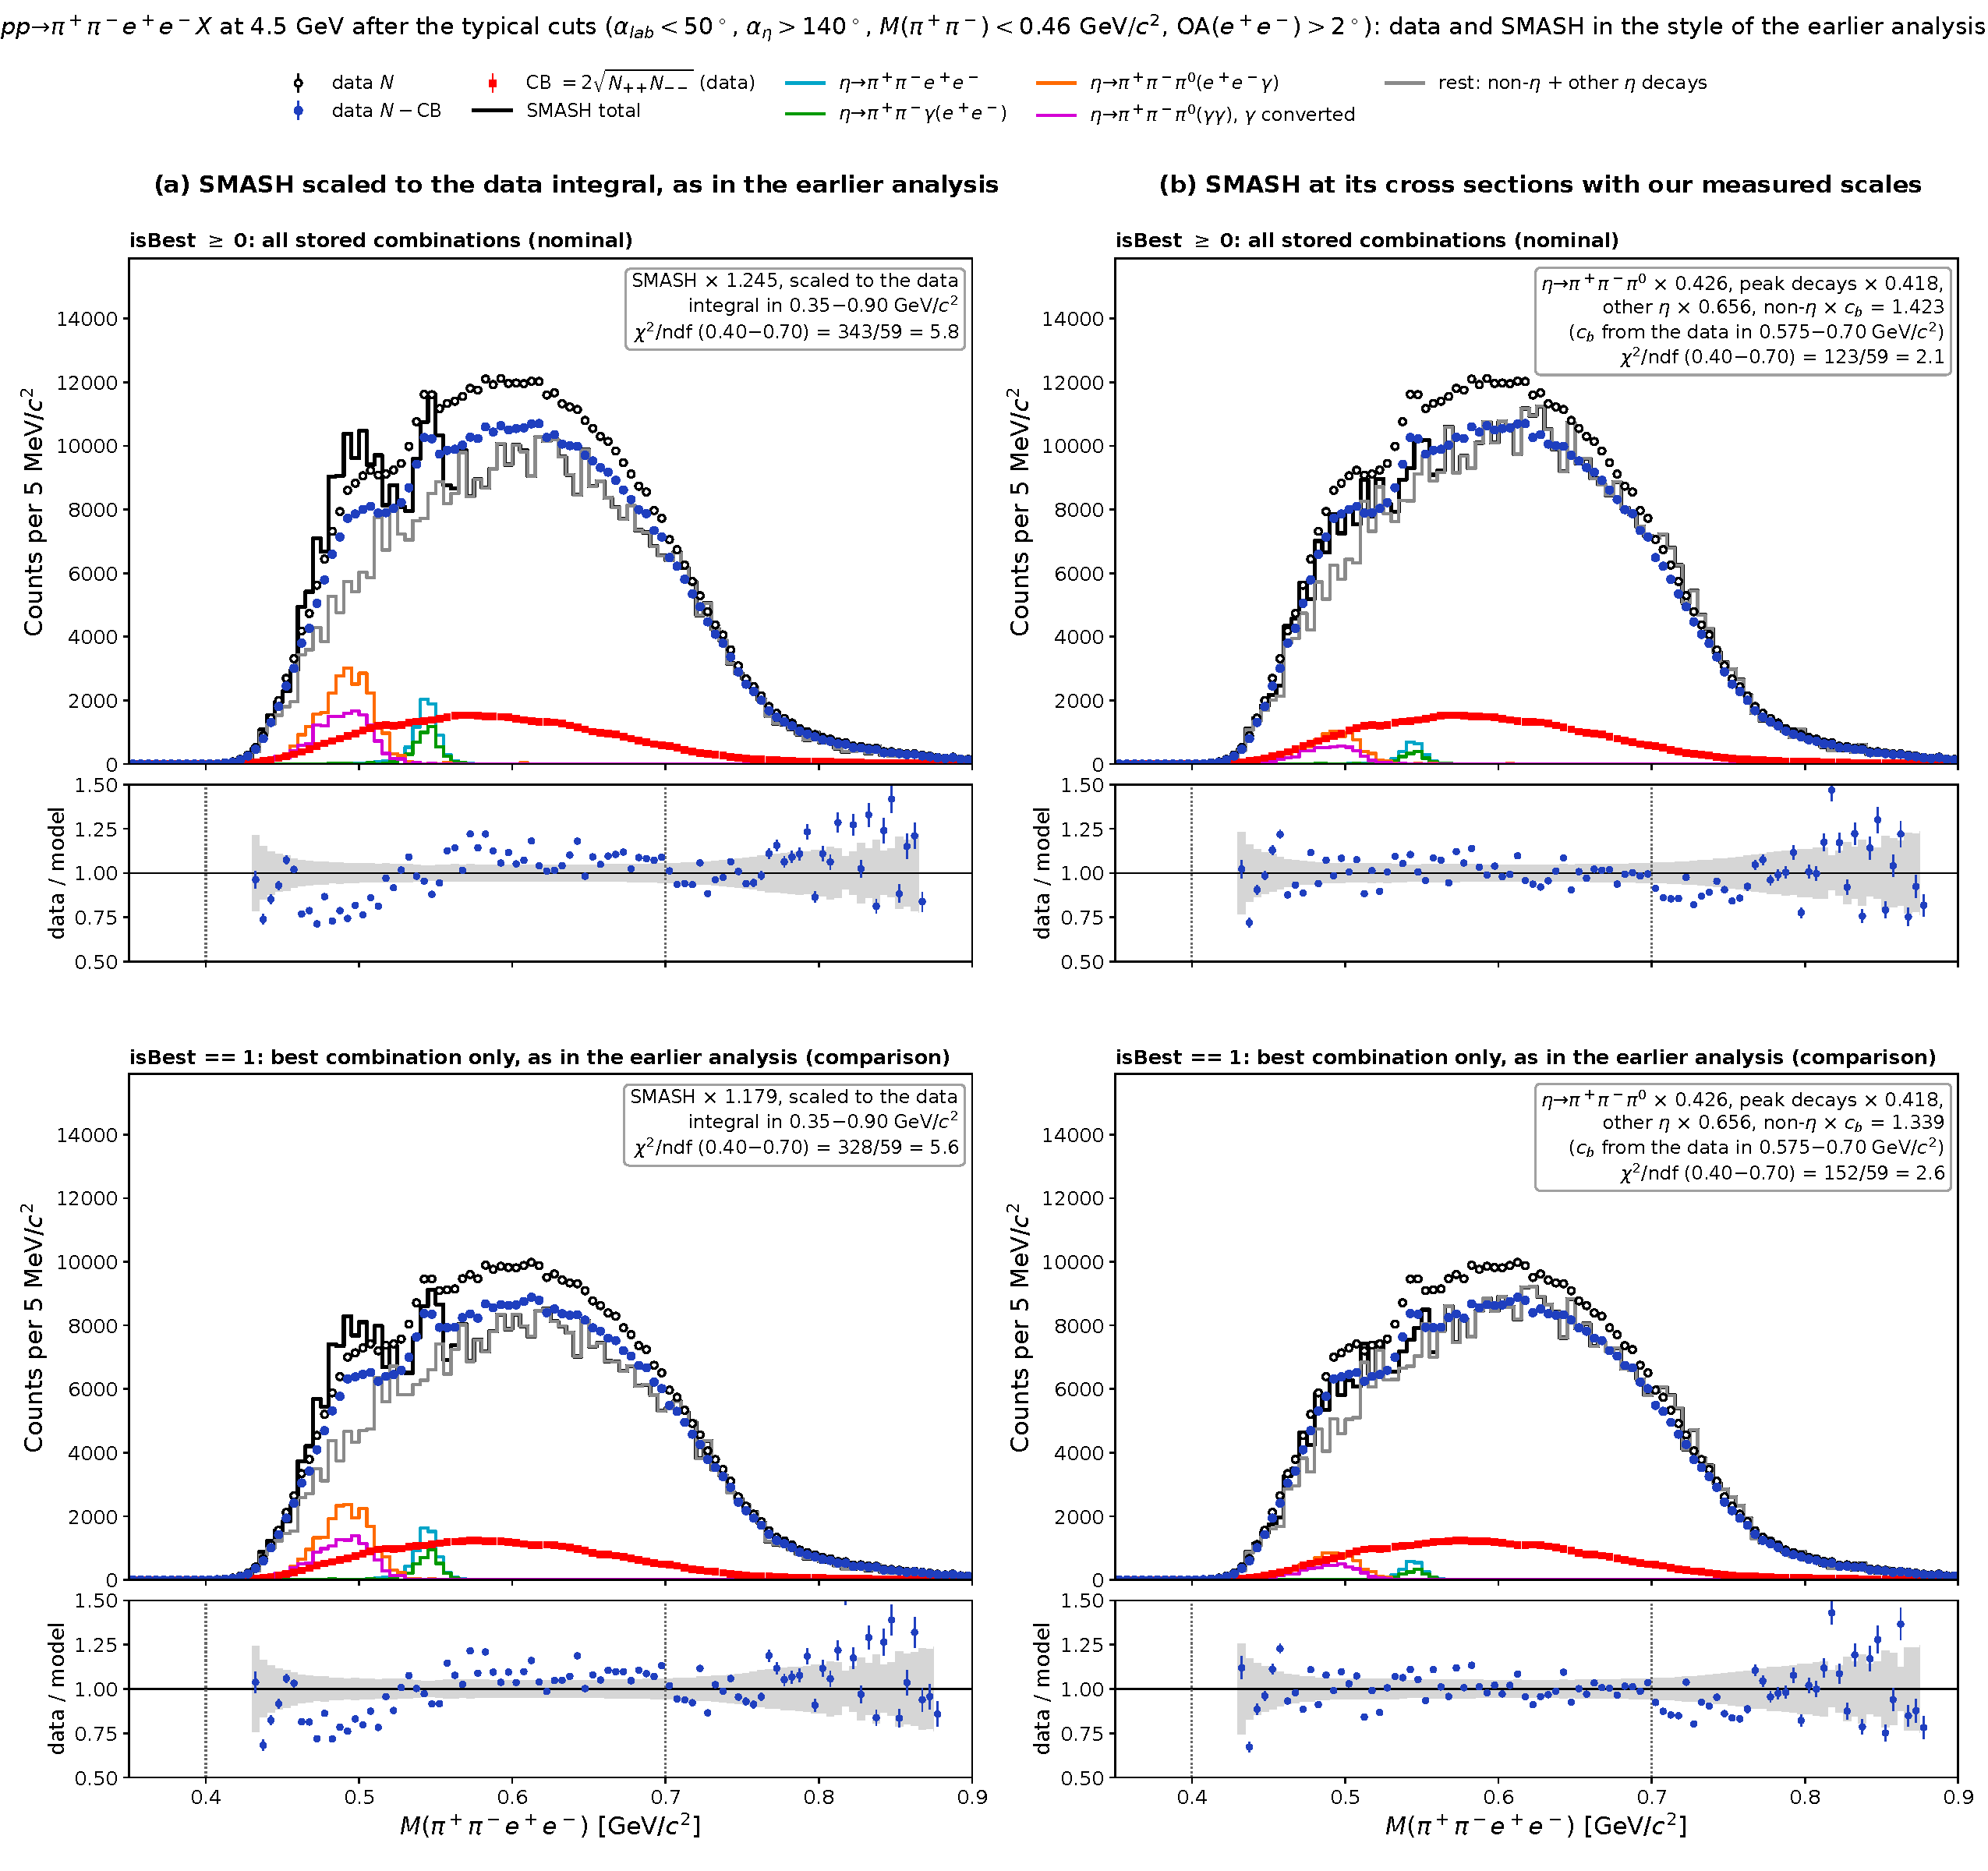
\includegraphics[width=0.84\textwidth]{figs_all/prevstyle_m4_E1.pdf}
\caption{\textbf{What it shows: SMASH scaled to the data integral, as in the earlier analysis, gets the total right but the parts wrong (bump
about 20\,\% too high, above the peak about 10\,\% too low; $\chi^2/\mathrm{ndf}=5.8$); with our measured scales it describes the data up to
0.70\,\GeVcc ($\chi^2/\mathrm{ndf}=2.1$).}
Selection: data and SMASH with the \ptthreecap{}, event vertex at $\vz>-160$\,mm, \betanew identification (pions $3\sigma$, leptons $5\sigma$ with a
RICH ring), energy-loss-corrected momenta, plus the typical cuts: angle between the \pipi and \ee systems below $50^\circ$ in the laboratory and
above $140^\circ$ in the $\eta$ rest frame, \Mpipi$<0.46$\,\GeVcc, \ee opening angle above $2^\circ$ (\cs{E1}); all \Mee. Top: all stored
combinations of each event (isBest $\ge0$, the nominal choice); bottom: the best combination only (isBest $=1$, in the data and in SMASH, shown
only to reproduce the earlier approach). Points: data $N$ (open), CB from the like-sign data (red), $N-\mathrm{CB}$ (blue), counts per
5\,\MeVcc; lines: SMASH total (black), the four $\eta$ decays (colours) and the rest (grey). (a) every SMASH line $\times$ one factor matched to the
integral of $N-\mathrm{CB}$ in 0.35--0.90\,\GeVcc, which hides the separate $\eta$ and background levels; (b) SMASH with our measured scales.
Same figure as Fig.~\ref{fig:e1-prev-m4} (\S\ref{sec:e1prev}), where the caption gives every detail. The demonstration with the background
fixed on the slope and two free $\eta$ scales (\S\ref{sec:e1prev}; not a measurement) gives, with the report's normalisation chain,
\sigeta$=0.47$\,mb from the bump and 0.67\,mb from the peak (measured: 0.444 and 0.429\,mb), and a one-window X17 count in the earlier style
gives $(5$--$8)\times10^{-5}$, anywhere between 1.6 and $13\times10^{-5}$ with reasonable side-band normalisations and $\eta$ scales (frozen
limit $3.16\times10^{-5}$).}
\label{fig:res-e1prev}
\end{figure}

%----------------------------------------------------------------------
\subsection{Checks that came out fine: the event-vertex cut and the target walls}
\label{sec:res-vtx}
The analysis keeps only combinations with an event vertex ($\vz>-500$\,mm, mandatory), which removes 32\,\% of the unlike-sign data counts but
almost none of the simulated ones. The cut keeps $0.994\pm0.021$ of the $\eta$ in the data (above 0.96 at 95\,\% CL; $0.990\pm0.022$ with the report's
CB convention) and 0.9997 in SMASH: the removed counts are mostly not hydrogen events (87\,\% of their pion pairs cross 8\,mm or more from the beam
axis; their source is probably material in front of the cell, a hypothesis) and hold no $\eta$. The cut is validated, and it is \emph{not} the
cause of the low \sigeta: 0.93\,mb would need an efficiency of 0.46, excluded at 23$\sigma$ by the ECAL-tagged $\eta$ (Fig.~\ref{fig:res-vtx}). The correction
$C_{\mathrm{vtx}}=1.006\pm0.021$ is not applied (one-sided $+2$\,\%, $+4$\,\% at 95\,\% CL). Likewise, the $\eta$ produced in the target walls
are only $3^{+4}_{-3}$\,\% of the $\eta$ signal (applied as the correction $1-\feta$, D21, approved by the analyst on 15 November 2026), although the walls give 13--15\,\% of the data
($N-\mathrm{CB}$) in 0.40--0.70\,\GeVcc (Fig.~\ref{fig:res-walls}). The small share of the $\eta$ is measured (Fig.~\ref{fig:res-feta}): in
vertex slices the $\eta$ per count falls to about zero where the walls give most of the counts, and the share of the $\eta$ in the centre of the cell ($0.566\pm0.045$ of $S$, $0.571\pm0.024$ of $T$) matches the LH$_2$ simulation (0.577).
\textbf{Status:} measured (after the review; the choices of the study approved by the analyst on 15 November 2026, D33). \textbf{Details:} \S\ref{sec:vertexeff},
\S\ref{sec:norm}.

\begin{figure}[!tbp]
\centering
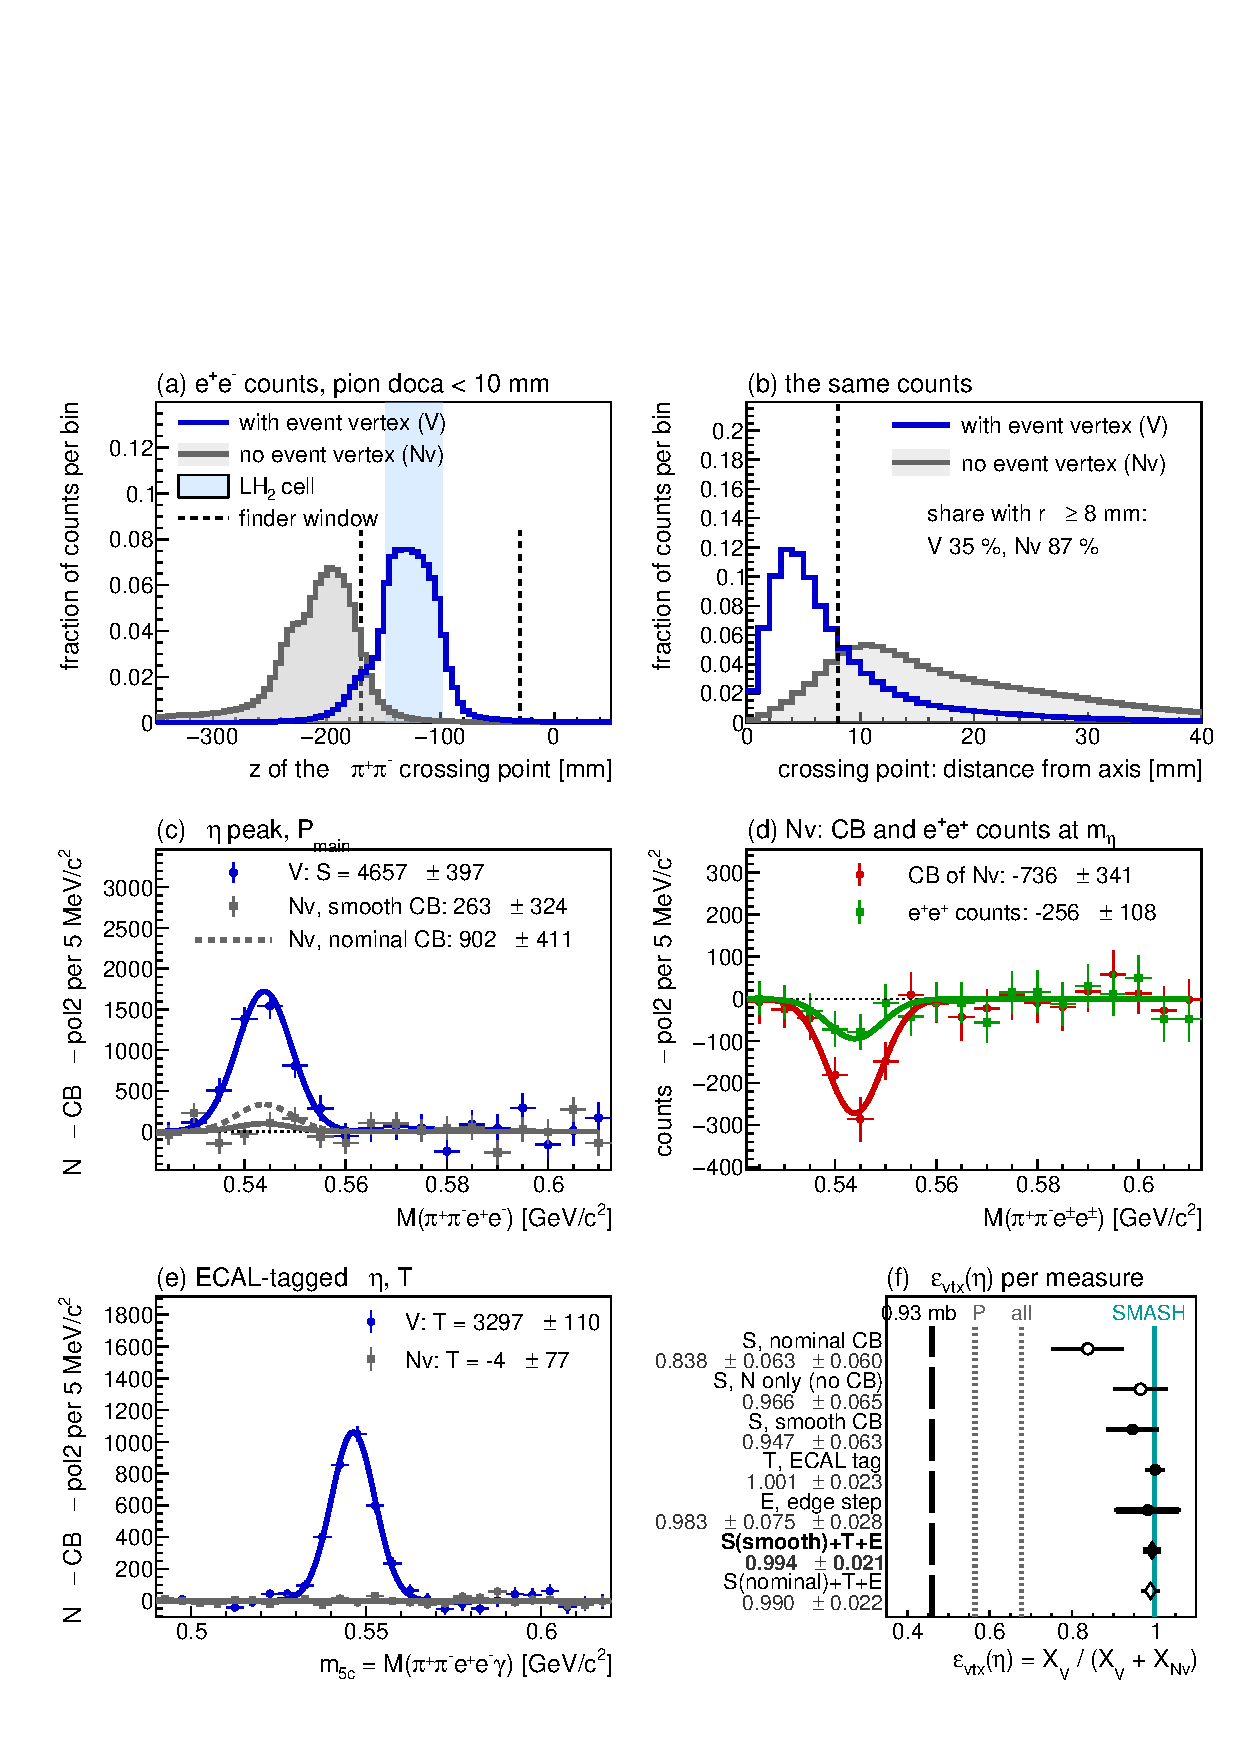
\includegraphics[width=0.86\textwidth,trim=0 0 0 428,clip]{figs_all/fix2_vtx_fig_cnt.pdf}
\caption{\textbf{What it shows: combinations without an event vertex hold no tagged $\eta$: the cut keeps the $\eta$.}
The combinations without an event vertex hold no tagged $\eta$ (e), so the vertex cut keeps practically all the $\eta$, far from the 0.46 that
$\sigeta=0.93$\,mb would need (f).
Selection: data of the 29 PAT day files: PT3 trigger, \betanew identification, corrected momenta, isBest $\ge0$, no target-region and no pion-vertex cut; events with (V, $\vz>-500$\,mm) and without (Nv) an event vertex, each with the CB of its own like-sign counts; (e) a good ECAL photon with $0.119\le M(\ee\gamma)<0.173$\,\GeVcc, \Mee$<0.10$\,\GeVcc, $m_{5c}$ fitted in 0.49--0.62\,\GeVcc; (f) $S$: \Pmain fit in \Mfour 0.5225--0.61\,\GeVcc; $E$: edge step in the four \Mpipi slices 0.30--0.34, 0.34--0.37, 0.37--0.39, 0.39--0.40\,\GeVcc.
Data, 29 PAT day files, PT3, isBest $\ge0$, \code{cor_ok}; combinations with an
event vertex (V, blue) and without one (Nv, grey). (e) ECAL-tagged $\eta$ in $m_{5c}=M(\ppee\gamma)$, $N-\mathrm{CB}-$pol2: $T=3297\pm110$
(V) and $-4\pm77$ (Nv). (f) $\varepsilon_{\mathrm{vtx}}=X_V/(X_V+X_{Nv})$ per measure ($S$ peak content, $T$ ECAL tag, $E$ edge step) and
combined, $0.994\pm0.021$ (open: not used for the result); lines: simulation 0.9997, survival of the counts 0.565 (P) and 0.677 (all), and 0.46,
needed for \sigeta $=0.93$\,mb. Bottom row of Fig.~\ref{fig:vtx}.}
\label{fig:res-vtx}
\end{figure}

\begin{figure}[!tbp]
\centering
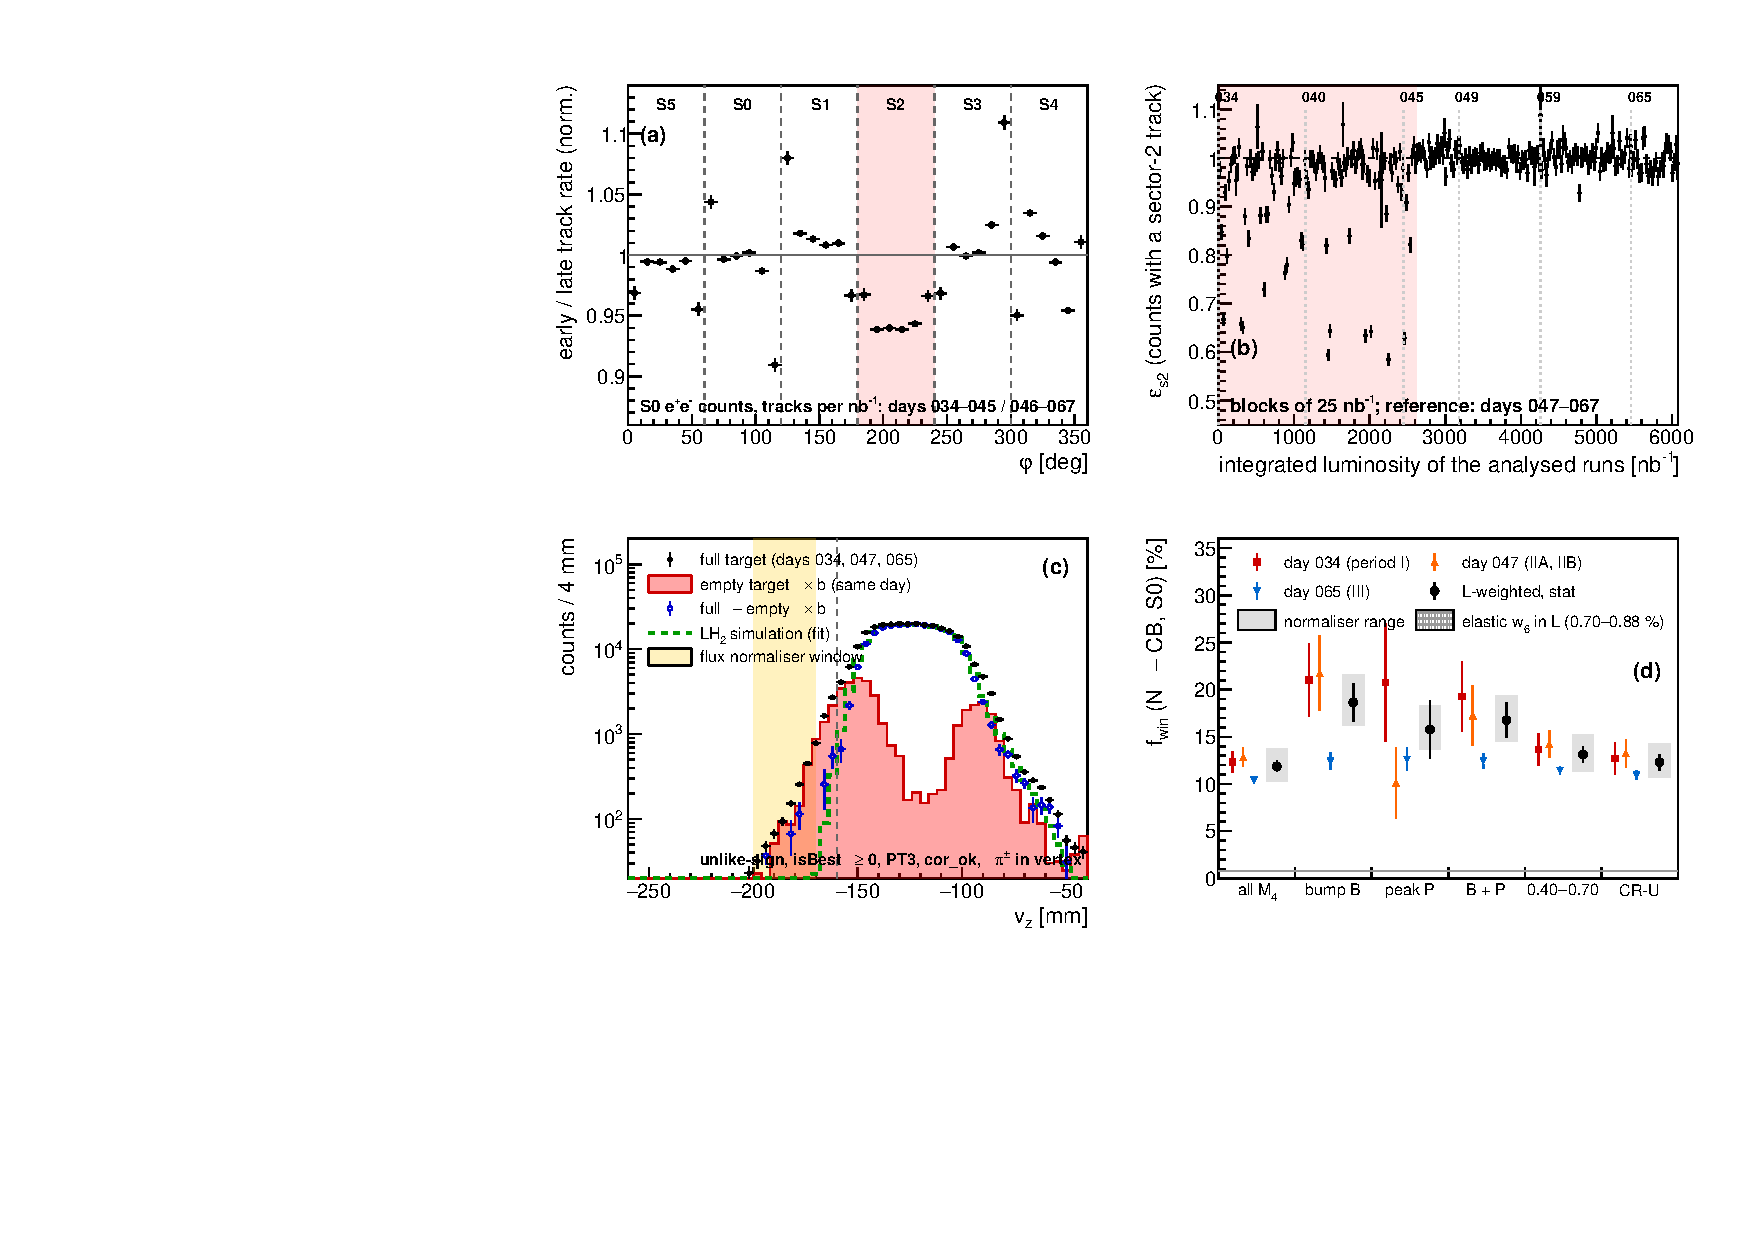
\includegraphics[width=0.80\textwidth,trim=0 0 0 220,clip]{figs_all/wp2_N1v2_cnt.pdf}
\caption{\textbf{What it shows: the target walls give 13--15\,\% of $N-\mathrm{CB}$, which SMASH does not simulate.}
The target walls (empty-target runs, red) give a visible part of the counts, 13--15\,\% of $N-\mathrm{CB}$ in 0.40--0.70\,\GeVcc.
Selection: (c) PT3 trigger, \betanew identification, corrected momenta, isBest $\ge0$, event vertex ($\vz>-500$\,mm) with both pions in its fit, no target-region cut, all \Mfour; days 034, 047, 065; flux ratio from the counts in $-200\le\vz<-170$\,mm. (d) S0 (PT3 trigger, event vertex at $\vz>-160$\,mm, \betanew identification (pions $3\sigma$, leptons $5\sigma$ with a RICH ring), corrected momenta, all stored combinations (isBest $\ge0$), both pions in the event-vertex fit) in the \Mfour windows: all, 0.4550--0.5225, 0.53364--0.55416, both, 0.40--0.70 and 0.565--0.700\,\GeVcc; CB of each window.
(c) Vertex $z$ of the unlike-sign combinations (isBest $\ge0$, PT3, \code{cor_ok}, both pions in
the vertex fit, all \Mfour), days 034 + 047 + 065: full target (black), empty target $\times\,b$ (red; flux ratio of the same day from the counts
in the shaded window $-200$ to $-170$\,mm), their difference (blue), LH$_2$ simulation fitted to the full-target profile (green); dashed: the
cut $\vz>-160$\,mm. (d) \fwin, the material share of $N-\mathrm{CB}$ in S0 per \Mfour window, per empty-target day and $L$-weighted
(statistical errors); 0.40--0.70\,\GeVcc: $13.1\pm0.9$\,\%. This is the share of all counts, mostly non-$\eta$ background; the share of the
$\eta$ signal, $3^{+4}_{-3}$\,\%, is shown in Fig.~\ref{fig:res-feta}. Bottom row of Fig.~\ref{fig:N1}.}
\label{fig:res-walls}
\end{figure}

\begin{figure}[!tbp]
\centering
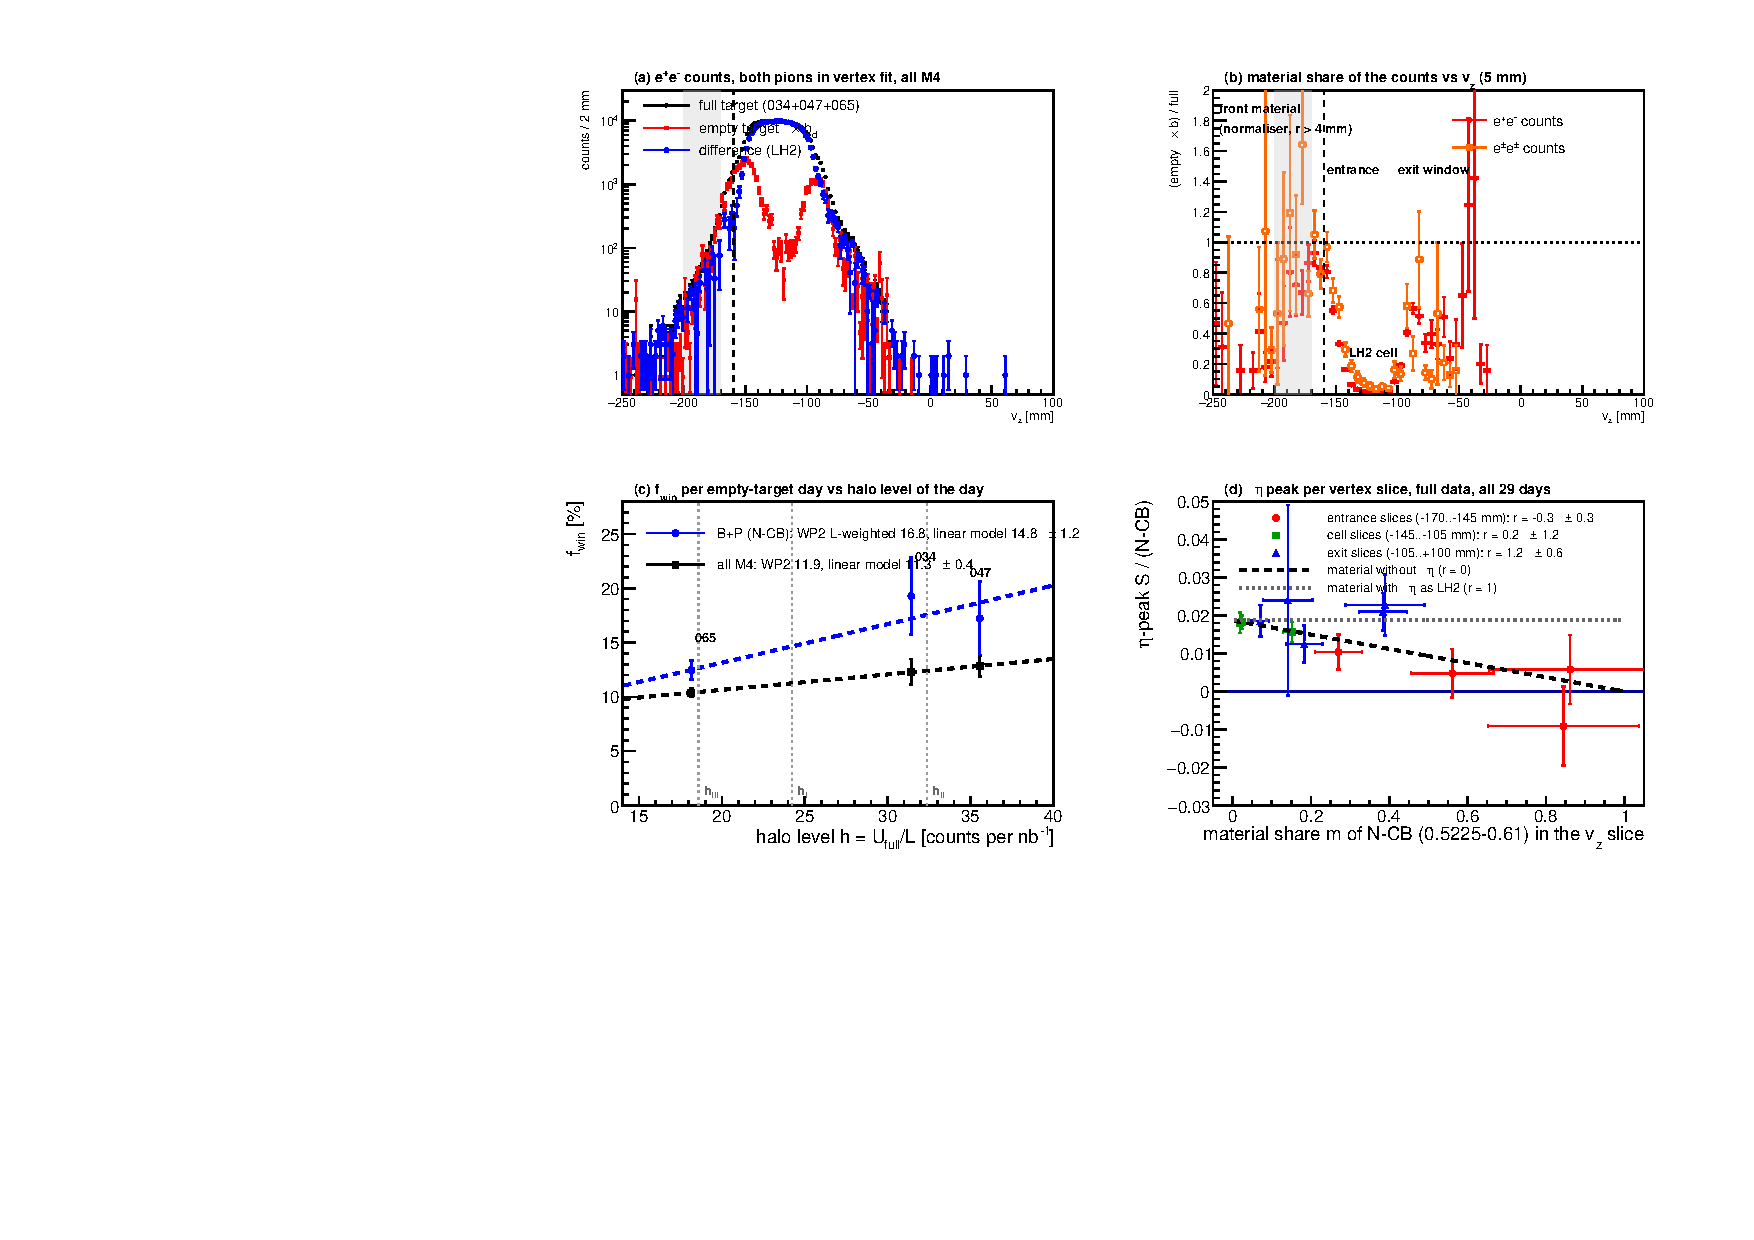
\includegraphics[width=0.86\textwidth]{figs_all/vw2a_fig_cnt.pdf}
\caption{\textbf{What it shows: the $\eta$ signal does not come from the target walls, so the $\eta$ yields are corrected by $1-\feta=0.97$ only, not by the wall share of the counts.}
Selection: data; PT3 trigger, \betanew identification, corrected momenta, isBest $\ge0$, event vertex ($\vz>-500$\,mm) with both pions in its fit, no target-region cut unless stated, all \Mfour. (a), (b) days 034, 047, 065, full and empty target; (c) S0 ($\vz>-160$\,mm added), bump and peak windows together (0.4550--0.5225, 0.53364--0.55416\,\GeVcc); (d) all 29 days, full target, 12 slices of $v_z$ from $-170$ to $+100$\,mm, $\eta$-peak content of a fixed Gaussian (0.5439\,\GeVcc, 5.4\,\MeVcc) + pol2 fitted in \Mfour 0.5225--0.61\,\GeVcc.
(a) Vertex $z$ of the \ee combinations (both pions in the vertex fit, all \Mfour), days 034\,+\,047\,+\,065: full target (black), empty target scaled by
the flux ratio of the same day (red), their difference (blue). (b) Material share of the counts per 5\,mm slice of $v_z$: the walls dominate at
the entrance window ($\approx-150$\,mm) and the exit window ($\approx-90$\,mm); inside the LH$_2$ cell they give about 1\,\%. (c) \fwin per
empty-target day against the beam-halo level of that day: \fwin follows the halo, and the empty-target days had a high halo; reweighted to the
luminosity-weighted halo, $\fwin(\mathrm{B+P})=14.7\pm1.1$\,\% instead of 16.8\,\%. (d) The decisive test, on the full data of all 29 days: the
$\eta$-peak content per $N-\mathrm{CB}$ count in each $v_z$ slice against the material share of that slice. If the walls produced no $\eta$, the
points would follow the dashed line (falling to zero at material share 1); if they produced $\eta$ like hydrogen, the dotted line. The
entrance-window slices (red), where the walls give 30--90\,\% of the counts, fall to about zero ($r=-0.27\pm0.34$ for these slices alone; exit-window
slices $r=1.21\pm0.64$); the fit of all slices gives the ratio of $\eta$ per count in the material to that in LH$_2$, $r=0.07\pm0.30$, i.e.\ a material share of the $\eta$ signal $f_\eta=3^{+4}_{-3}$\,\% (adopted, D21, approved by the analyst on 15 November 2026; 1--8\,\%
over the vertex models). An independent check agrees: the share of the $\eta$ peak and of the ECAL-tagged $\eta$ in the cell centre,
$0.566\pm0.045$ and $0.571\pm0.024$, equals the LH$_2$ simulation (0.577), whereas an $\eta$ material share of 16.8\,\% would give 0.497
(excluded at $3.4\sigma$). Figure of the independent verification of WP2 (vw2a).}
\label{fig:res-feta}
\end{figure}

%----------------------------------------------------------------------
\subsection{A defect of the simulation}
\label{sec:res-qed}
HGeant, used for the standard SMASH set, decays the virtual photon of $\piz\to\gamma\ee$ isotropically instead of with the QED distribution
$1+\cos^2\theta^*$ (PLUTO, used for the lepton set, has the right angle). For the bump counts of this analysis the
simulated efficiency of class C2 is therefore about 16\,\% too high: the per-count QED weights of the full simulation give 0.86 at the bump
edges. Toys with a sharp 60\,\MeVc lepton threshold and the lepton/standard closure of prompt \piz Dalitz pairs gave
$\varepsilon_{\mathrm{QED}}/\varepsilon_{\mathrm{iso}}=0.875$--0.891 (12--14\,\%, confirmed independently); the closure 0.891 of Part~I, left
unexplained there, is explained as the closure of prompt \piz pairs. \sigeta from the peak is unchanged (Fig.~\ref{fig:res-qed}). At the bump edge
the factor was first checked with a new toy (0.883 at the edge against 0.880 over all \Mfour), and the constant factor 0.8855 (the mean of toy and
closure, effective 0.881; D35) was applied. A per-count average of the QED weight along the circle on which each lost photon must lie then gave
0.861 ($u$) and 0.860 (per slice) at the edges; the analyst approved these per-count weights on 15 November 2026 (D38; an independent verifier
confirms them to 0.0004), to be applied until a future simulation corrects the angle in GEANT itself (not expected). C2 makes more than half of
the simulated step, and the correction raises the edge scale by 9.2\,\% in $u$, from 0.390 to 0.426, and by 8.1\,\% per slice, from 0.392 to
0.423 (\S\ref{sec:c2recon}).
\textbf{Status:} measured on the simulation; not applied in the frozen Part~III numbers, where it enters as a known-sign systematic; applied,
count by count, to the bump-edge values (D35, D38). \textbf{Details:} \S\ref{sec:eff}, \S\ref{sec:bedge-c2}.

\begin{figure}[!tbp]
\centering
\begin{minipage}[c]{0.36\textwidth}
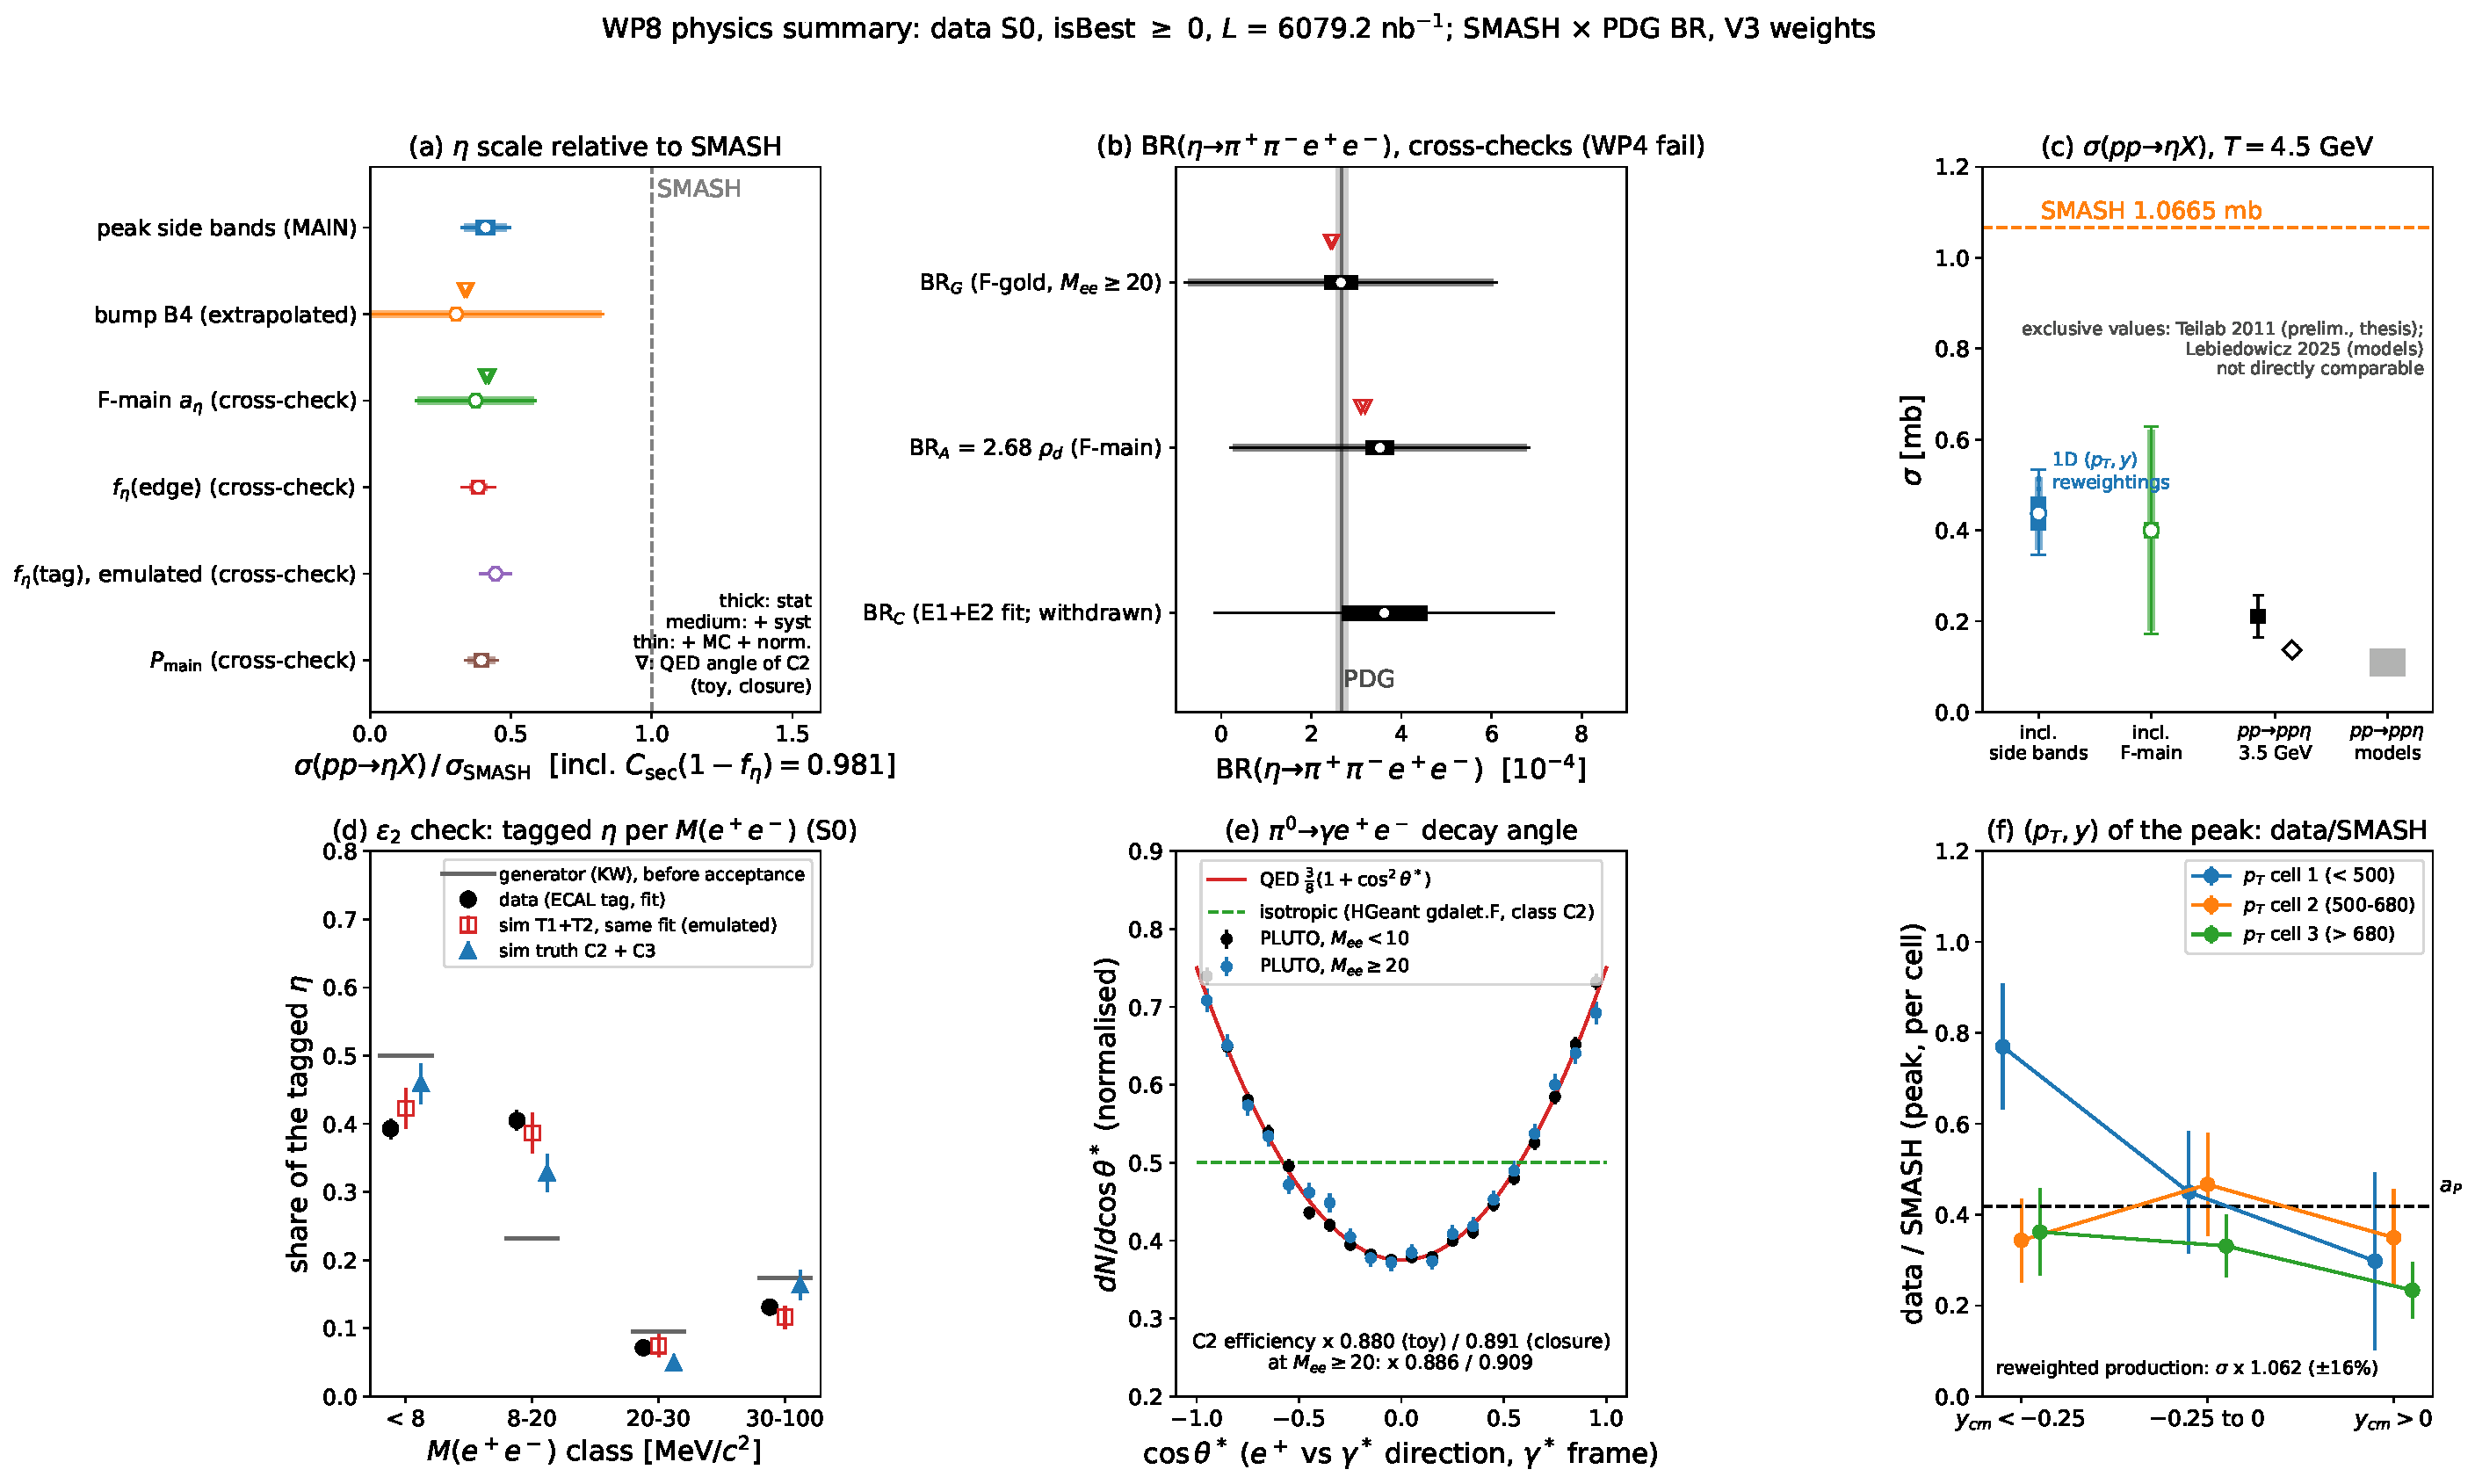
\includegraphics[width=\textwidth,trim=585 0 440 442,clip]{figs_all/wp8_P1.pdf}
\end{minipage}\hfill
\begin{minipage}[c]{0.61\textwidth}
\caption{\textbf{What it shows: HGeant decays the $\gamma^*$ isotropically; QED wants $1+\cos^2\theta^*$.}
The decay angle must follow QED, $1+\cos^2\theta^*$ (red line, PLUTO points), but HGeant decays the $\gamma^*$ isotropically (flat green
line).
Selection: no event selection: the generator-level PLUTO $\piz\to\gamma\ee$ decays of the lepton set (124\,k decays), \Mee below 10 and from 20\,\MeVcc; the HGeant curve from its decay code (class C2).
Decay angle of
$\piz\to\gamma\ee$ ($e^+$ against the $\gamma^*$ direction, in the $\gamma^*$ frame) in PLUTO (lepton set, 124\,k decays; black
\Mee$<10$\,\MeVcc, blue \Mee$\ge20$\,\MeVcc) against QED $(3/8)(1+\cos^2\theta^*)$ and the isotropic decay of HGeant (class C2). For the
bump counts the simulated C2 efficiency is about 16\,\% too high (per-count QED weights of the full simulation, 0.86 at the edges, D38); the
toys and the closure of prompt \piz pairs gave 12--14\,\% ($\varepsilon_{\mathrm{QED}}/\varepsilon_{\mathrm{iso}}=0.875$--0.891: 0.880 from
the toy, 0.891 from the closure, 0.875 from the verifier's toy). Panel (e) of Fig.~\ref{fig:P1}.}
\label{fig:res-qed}
\end{minipage}
\end{figure}

%----------------------------------------------------------------------
\subsection{What is not determined, and why}
\label{sec:res-notdet}
\begin{itemize}\setlength{\itemsep}{1pt}
\item \textbf{The background-subtracted area of the bump (B4) and the double ratio derived from it}: the background under the bump can only be
      extrapolated from above the peak; no control region with a known bump-free shape exists below it (157\,\%; \S\ref{sec:b4};
      Figs.~\ref{fig:res-peak}a, \ref{fig:res-after}). The bump itself is \emph{not} in this list any more: it is measured through its kinematic
      edge, with its own double ratio $\mathrm{DR}_u=0.97\pm0.37$, which includes the composition term of the peak
      ($\mathrm{DR}_{\mathrm{edge}}$ of the per-slice edge: $\pm0.24$ without it) (\S\ref{sec:res-bump}).
\item \textbf{BR$(\eta\to\ppee)$}: the template fits give $\BRG=2.67\times10^{-4}$, consistent with PDG ($2.76\pm0.16$), but they failed the
      pseudo-data test (the noisy simulated signal templates bias them by about $-10$\,\%) and the total uncertainty is about 130\,\%: a
      cross-check, not a measurement (\S\ref{sec:fit}; Fig.~\ref{fig:res-p1}b).
\item \textbf{The make-up of the $\eta$ peak}: the direct decays give an $\eta$ scale of 0.50 of SMASH, the converted photons 0.24; which SMASH
      component is wrong (simulated material and close-pair efficiency, or the direct-decay rate) is not known. It sets \sigeta between 0.25
      and 0.52\,mb (\S\ref{sec:p2}; Fig.~\ref{fig:res-p1}a, c). It is taken from the data, provisionally (D31), until the separate close-pair
      analysis of D32. The bump edge does not decide it either: 0.426 of SMASH in $u$ (0.423 per slice) with the simulated conversion rate,
      0.549 (0.569) with the conversions $\times0.48$; its own \Mee split gives $\kappa=0.83\pm0.20\pm0.34$, consistent with 1 and with 0.48
      (\S\ref{sec:res-bump}).
\item \textbf{The full reconstruction of the bump with the ECAL photon} as a measurement: today a feasibility study, limited by the photon
      energy scale and the module efficiency (\S\ref{sec:res-ecal}).
\item \textbf{The split of the non-$\eta$ background, and the per-channel SMASH scales as measurements}: in the flexible description the
      background above the peak is 10--30\,\% above SMASH, but $G_D$, $G_C$ and \Geta are 80--90\,\% correlated and move with the fit method;
      the per-channel scales are a documented description, not measurements (D36; \S\ref{sec:res-flex}).
\item \textbf{Pairs with \Mee$<10$\,\MeVcc} (class E1) are not described (their combinatorial background would need a factor 7.6--13.2; the stage-A
      background carried to them puts SMASH with the measured scales 1/0.65 too high in $u$, \S\ref{sec:res-bump}); they are left out of every fit, and the all-\Mee yields are extrapolated with the simulated \Mee shape (\S\ref{sec:step0}).
\item \textbf{The significance} of the difference between \sigeta and the HADES values at 3.5\,GeV is not quoted, because the make-up of the
      peak is unresolved (\S\ref{sec:lit}).
\end{itemize}

%----------------------------------------------------------------------
\subsection{A possible explanation, to be tested in a separate analysis (D32)}
\label{sec:res-d32}
The analyst proposes that the data lose close \ee pairs (small opening angle, small \Mee) more often than the simulation does. The classes made
of close pairs give lower $\eta$ scales than the direct decays, whose pairs spread to large \Mee (converted photons $0.237\pm0.049$, direct
decays $0.497\pm0.059$, stat; Fig.~\ref{fig:res-p1}a), and the data peak has more pairs above 10\,\MeVcc than SMASH (share $0.546\pm0.053$ against 0.425, 2.3$\sigma$).
The bump, also made of close pairs, gives 0.426 in $u$ (0.423 per slice) with the simulated conversion rate and 0.549 (0.569) with the
conversions $\times0.48$, so it does not decide (\S\ref{sec:res-bump}). If this holds, the direct decays give the most reliable $\eta$ scale, and
\sigeta $\approx0.52\pm0.06\,(\mathrm{stat})$\,mb. The evidence is suggestive, not conclusive, and no number of this report is changed.
\textbf{Ruled by the analyst on 15 November 2026 (D32):} the interpretation stays to be tested, in a \emph{separate} analysis that is not part
of these reports: the reconstruction efficiency of \ee pairs with an opening angle of 0--6$^\circ$ in data and simulation, measured with \piz,
$\eta$ and $\omega$ Dalitz decays (the \ee hypothesis plus the ECAL photon). It waits for the trigger-bias correction and the new ECAL calibration
(both in progress); its results will be brought into these reports. Until then the make-up of the peak is taken from the data, provisionally
(D31, \S\ref{sec:res-sigma}).

\subsection{Open questions}
\label{sec:res-open}
\begin{enumerate}\setlength{\itemsep}{1pt}
\item The close-pair efficiency of data against simulation: the separate analysis of D32 (pairs with OA 0--6$^\circ$ from \piz, $\eta$ and
      $\omega$ Dalitz decays with the ECAL photon; after the trigger-bias correction and the new ECAL calibration), now the largest open item of
      every absolute statement.
\item The simulation statistics, which limit every template fit, B4, the bump edges (MC error 7.0\,\% in $u$ against 4.7\,\% statistical; twice
      the statistical one per slice) and the flexible description (MC error 1--8 times the statistical one): a larger standard-set production
      is requested, and a forced $\eta\to\pipi\piz$ production with the full ECAL simulation, at least 10 times the present statistics. Taking
      the simulated step from the bump classes alone (no smoothing model) gives MC 7.0\,\% in $u$ and about 6.6\,\% per slice; the $u$-edge does
      this.
\item The full reconstruction with the ECAL photon: requirements (1)--(4) of \S\ref{sec:res-ecal} (photon energy scale and resolution, module
      efficiency, a START-free photon cut, more simulation); it connects with the separate ECAL analysis of D32.
\item A control region below the peak with a known bump-free shape, needed for the bump area B4 (the bump yield itself now comes from the edge).
\item The low-mass tail of the $\eta$ peak near the bump edge (D40, \S\ref{sec:edgeu-tail}): the tail is the leptons' radiation in the
      material (HGeant) and is certainly present, but the data do not measure its size ($t=0.3\pm1.0$ of the simulated tail): the peak position
      and the 180 simulated $\eta\to\pipi\gamma$ conversion entries limit the test. No tail would lower $f_\eta(u\text{-edge})$ by 6.9\,\% and the
      per-slice edge by 7\,\%. The term for $t=1\pm0.5$, $\pm3.4$ / $\pm3.6$\,\%, is counted (D40, approved). A larger simulated $\eta\to\pipi\gamma$ sample and a simulation
      with final-state radiation would settle it.
\item The QED decay angle of class C2: the bump edges use per-count QED weights (0.861 in $u$, 0.860 per slice; D38, approved,
      \S\ref{sec:c2recon}), to be applied until a future simulation corrects the angle in GEANT itself, which is not expected.
\item Why scaled SMASH components do not describe the spectrum (flexible model $p<0.001$; no description above \Mfour$=0.70$\,\GeVcc); one
      candidate is the target material that SMASH does not simulate (13--15\,\% of $N-\mathrm{CB}$).
\item The production model: the $p_T$/$y$ item of \sigeta ($^{+19}_{-7}$\,\%) is kept separate from the total (ruled, D29: $^{+0.08}_{-0.03}$\,mb).
      Still pending is the ruling on the
      ``ghost'' pairs (D6): whether simulated true pairs whose tracks carry the ghost flag count as real pairs (variant (a); it moves the
      ratios of \S\ref{sec:res-before} by 8.5--14.5\,\%).
\item The \Mee scale and resolution of the X17 line (not checked on the data); the vertex condition of the elastic luminosity (about 1\,\% if none).
\end{enumerate}
The full list with the details is in \S\ref{sec:concl}.

%----------------------------------------------------------------------
\subsection{Decisions: D21--D40 ruled on 15 November 2026; deviations within D1--D20 still open}
\label{sec:res-decisions}
The decisions D1--D20 were fixed in the specification before any yield was seen; D21--D33 were taken during the analysis or the review,
D34 with the comparison after the typical cuts, D35 and D36 with the bump-edge measurement and the flexible SMASH description, D37--D39 with
the $u$-edge, the C2-factor check and the like-sign step, and D40 with the tail of the $\eta$ peak. D21--D40 were
all ruled by the analyst on 15 November 2026 (D22--D24, D30, D33 and D37--D40 approved in the evening, D40 with option (a)); only the deviations
and fall-backs among D1--D20 await the analyst. The most consequential ones (the full table
with reasons and status is App.~\ref{sec:decisions}):
\begin{itemize}\setlength{\itemsep}{1pt}
\item \textbf{D22} (approved), the pass/fail rule of the pseudo-data test: pseudo-data with realistic template noise (``method
      configurations + RF'') instead of the specified half-sample test BA, chosen after the BA results were seen (under BA every estimator fails).
\item \textbf{D23} (approved): D11 and the stage-A $\chi^2$ criterion are judged with the template covariance (GLS).
\item \textbf{D24} (approved), two systematics rules taken after the variants were seen: the template noise of a variant shift is
      subtracted (MC($\Delta$)), and variants that the data reject are not counted (rule R1): \Ypeak systematic 11.5\,\% instead of 15.2\,\%.
\item \textbf{D31} (ruled, option (a)): the make-up of the peak is taken from the data instead of the prior (\sigeta 0.43\,mb, systematic
      35.5\,\% instead of 18.5\,\%), \emph{provisionally} until the test of D32; if that test confirms a loss of close pairs in the data, the
      direct-decay route (0.52\,mb) becomes the natural headline with a much smaller composition term.
\item \textbf{D32} (ruled): the close-pair interpretation stays to be tested, in a separate analysis (pairs with OA 0--6$^\circ$ from \piz,
      $\eta$, $\omega$ Dalitz decays with the ECAL photon; after the trigger-bias correction and the new ECAL calibration).
\item \textbf{D21} (approved): Amendment~1, $\eta$ yields use $1-\feta$ (wall share of the $\eta$), never $1-\fwin$: \sigeta $+17$\,\%.
\item \textbf{D25} (ruled): PDG 2026 everywhere, also for the X17 limit: $\BRX<3.16\times10^{-5}$ ($r<0.114$); the frozen value with PDG 2020,
      $3.06\times10^{-5}$, in a footnote.
\item \textbf{D26} (approved): sector-2 deficit span 034--045 for \Csec ($+0.1$\,\%); the elastic events of day 045 have no sector-2 deficit
      (PT2 and PT3), so $L$ is unchanged (\S\ref{sec:norm}).
\item \textbf{D27} (approved): $\eta_{\mathrm{U}}$ subtracted in B4 before the extrapolation.
\item \textbf{D28} (ruled): \sigeta keeps the PRELIMINARY label, because the make-up of the peak is open ($\pm32$\,\%); its first reason,
      the event-vertex efficiency, is measured.
\item \textbf{D29} (ruled): the production-model item stays separate from the total: $\sigeta=0.43\pm0.17\,^{+0.08}_{-0.03}\,(\mathrm{model})$\,mb (with the peak-tail term of D40).
\item \textbf{D30} (approved: normalisation (1) primary, (2) quoted next to it), X17 normalisation (1) kept although it failed the slope test on the specified toys: $3.16$ (3.06 with
      PDG 2020), not $3.29\times10^{-5}$.
\item \textbf{D33} (approved), choices of the vertex study (smooth like-sign CB, three measures combined, no correction): $0.994$, not
      $0.990$.
\item \textbf{D34} (ruled 15 November 2026): the typical $\eta$/X17 cuts are \emph{not} applied, because the numbers show they do not help
      (\S\ref{sec:e1}); the variants with the cuts stay shown with their numbers.
\item \textbf{D35} (lead analysis, approved 15 November 2026): the bump-edge scale is quoted \emph{with} the C2 $\gamma^*$-angle correction as the recommended value
      (0.418; 0.437\,mb with the constant factor; 0.423; 0.442\,mb with the per-count weights of D38), and \emph{without} it (0.392; 0.409\,mb) for comparison with the frozen convention (WP8: a known-sign systematic).
\item \textbf{D36} (lead analysis, approved 15 November 2026): the flexible SMASH model was chosen with three conditions added after the first ladder result; the
      per-channel scales are a documented description, not measurements.
\item \textbf{D37} (lead analysis, approved 15 November 2026): the $u$-edge is \emph{the} bump measurement (0.426; \sigeta from the bump
      0.444\,mb), the per-slice edge (D35) the cross-check; the headline \sigeta $=0.429$\,mb from the peak side bands is unchanged.
\item \textbf{D38} (lead analysis, approved 15 November 2026): the constant C2 factor of the bump edges is replaced by per-count QED weights
      (effective 0.861 / 0.860 instead of 0.881), to be applied until a future simulation corrects the angle in GEANT itself (not expected);
      $f$ and \sigeta from the bump $+1.4$\,\% ($u$: 0.426, 0.444\,mb) / $+1.2$\,\% (per slice: 0.423, 0.442\,mb); allowance
      $\pm0.024\to\pm0.004$; the factors are confirmed by an independent verifier to 0.0004.
\item \textbf{D39} (lead analysis, approved 15 November 2026; independently verified, wording corrected): the $e^-e^-$ like-sign step at the edge
      (4.7$\sigma$) is recorded as lepton pairs from the two \piz photons of $\eta\to\pipi\piz$, seen mostly as $e^-e^-$ because of the $e^+$/$e^-$
      acceptance and of Compton/knock-on electrons (negative only), not a charge flip ($<1.2$\,\%, 90\,\% CL); the CB and U5 (2.6\,\%) are kept
      (data test $k_{\mathrm{cross}}=1.00\pm0.39$; independent, with the constant C2 factor, $0.96\pm0.48$); the caveat ``up to $+8$\,\%'' is replaced by the flip limit
      ($<+1.6$\,\% on $f$; $<+1.9$\,\% for either charge) and the $k_{\mathrm{cross}}$ check ($0.0\pm1.2$\,\%); no headline number changes.
\item \textbf{D40} (lead analysis, approved 15 November 2026, option (a)): the low-mass tail of the $\eta$ peak term (the leptons'
      radiation in the material, HGeant) is kept as simulated ($t=1$) and gets a systematic family ``peak tail'' with $t=1\pm0.5$ (a physics
      band; the data allow $0.3\pm1.0$): $f_\eta(u\text{-edge})$ $\pm3.4$\,\% (U8 merged; total 11.1 $\to$ 11.6\,\%), $f_\eta(\mathrm{edge})$
      $\pm3.6$\,\% (3.7\,\% with the per-count C2 weights; total 15.0 $\to$ 15.4\,\%), \aP and \sigeta from the peak side bands $\pm8.8$\,\%: the
      headline becomes $\sigeta=0.43\pm0.17\,(\mathrm{measurement})\,^{+0.08}_{-0.03}\,(\mathrm{model})$\,mb, PRELIMINARY; no central value changes.
\end{itemize}
The earlier front-page summary with every condition and variant of the main results is App.~\ref{app:status}.

%----------------------------------------------------------------------
\par\ifdim\dimexpr\pagegoal-\pagetotal\relax<8\baselineskip\newpage\fi% keep the heading with its table (no heading alone at the page foot)
\subsection{Symbols used in this section}
\label{sec:symbols1}
{\footnotesize
\renewcommand{\arraystretch}{1.0}
\begin{longtable}{@{}>{\raggedright\arraybackslash}p{3.3cm} >{\raggedright\arraybackslash}p{\dimexpr\textwidth-3.3cm-2\tabcolsep\relax}@{}}
\toprule
count & one stored \ppee combination (one ntuple entry); with isBest $\ge0$ an event can give more than one count \\
S0, isBest $\ge0$ & nominal selection (event vertex, both pions in the vertex fit); all stored combinations of an event are kept \\
$N$, CB & unlike-sign data counts; combinatorial background, $2\sqrt{N_{++}N_{--}}$ from the like-sign data counts ($\pipi e^+e^+$, $\pipi e^-e^-$) \\
\Mfour, \Mee & invariant mass of the four tracks; of the \ee pair \\
$L$ & luminosity of the analysed runs, 6079.2\,\nbinv ($\pm6.9$\,\%) \\
\Ypeak, \aP & $\eta$ peak yield in counts ($\times64/63$ for the trigger bit); \Ypeak divided by the SMASH expectation \\
B4, \Ybump & side-band estimator of the bump area (not determined) and its bump yield; the yield from the edge is \Ybump(edge) \\
$u$, $E(m,q)$ & distance to the kinematic edge of the bump, $u=\Mfour-E(\Mpipi,\Mee)$; the edge $E$ itself (exact, with the \Mee term,
Eq.~\ref{eq:edge}) \\
$f_\eta(u\text{-edge})$, DR$_u$ & $\eta$ scale of the bump: step height at $u=0$, data/SMASH with one fit ($h_{\mathrm{data}}/h_{\mathrm{sim}}$);
double ratio $\aP/f_\eta(u\text{-edge})$, with the composition term of the peak \\
$f_\eta(\mathrm{edge})$, DR$_{\mathrm{edge}}$ & the same from the per-slice edge in \Mfour (Part~II's measure $E$; cross-check); double ratio
peak/bump $\aP/f_\eta(\mathrm{edge})$, without the composition term \\
$\kappa$ & scale of the simulated conversion pairs relative to the Dalitz and direct pairs ($\kappa=1$: SMASH as is) \\
cross-photon pair, $k_{\mathrm{cross}}$ & pair of leptons from the two different photons of the \piz in $\eta\to\pipi\piz$; they make the
like-sign step at $u=0$; their scale in $N$ relative to the CB rule (1 = the rule) \\
peak tail, $t$ & low-mass tail of the simulated $\eta$ peak (combinations whose leptons lost enough momentum in the material to shift \Mfour by more
than 5\,\MeVcc); $t$ scales it ($t=1$: SMASH as is, $t=0$: no tail) \\
F8; $s_X$; $\lambda$ & nominal flexible SMASH fit (8 free scales); its scale of component $X$; weight of the template noise in the fit weights
($\lambda=1$ nominal) used to test the fit method (in Fig.~\ref{fig:res-udatasim} $\lambda$ is instead one free factor on $G_D+G_C$) \\
$G_D$, $G_C$, \Geta; \kB & SMASH classes: non-$\eta$ Dalitz and vector-meson pairs; non-$\eta$ conversion pairs; other $\eta$ decays; the
conversion scale on $G_C$ of the stage-A background normalisation (fitted for \Mee$\ge10$\,\MeVcc) \\
\Pmain; ECAL tag & Part~II's fit of the $\eta$ peak; $\eta\to\pipi\piz$ combinations tagged by an ECAL photon with $M(\ee\gamma)$ in
0.119--0.173\,\GeVcc, around the \piz mass (Part~II's $T$; the simulated tag is emulated, its acceptance verified, its photon-energy
scale not) \\
C2, C3, C4, C5 & $\eta$ classes: bump via \piz Dalitz; bump via a converted photon; $\eta\to\pipi\gamma$ with a converted photon; direct $\eta\to\ppee$ \\
\sigeta & inclusive $\eta$ production cross section in p+p at 4.5\,GeV \\
$\varepsilon_{\mathrm{vtx}}$, $C_{\mathrm{vtx}}$ & $\eta$ efficiency of the event-vertex cut $\vz>-500$\,mm; the correction simulation/data (not applied) \\
\feta, \fwin & share of target-wall (empty-target) events in the $\eta$ signal; in all $N-\mathrm{CB}$ counts \\
\BRG & BR$(\eta\to\ppee)$ from the template fit of \Mee$\ge20$\,\MeVcc (F-gold) \\
live time, sorter, \code{cor_ok} & one-sided items, not applied: trigger live fraction; event loss of the START-based DST track sorter; flag of
the combinations with corrected momenta (combinations with \code{cor_ok}$\,=0$ are dropped) \\
BA; AA, BB; RF; RB & pseudo-data (closure) configurations: BA (specified) truth from one half of the simulation, templates from the other;
AA, BB (``method'') truth and templates from the same half; RF truth from the full sample, templates from bootstrap replicas (realistic
template noise); RB: RF with a bias correction. Adopted rule: AA, BB + RF (D22) \\
MC($\Delta$), R1 & systematics rules of work package WP7: template noise of a variant shift subtracted; variants rejected by the data not counted \\
ghost, variant (a) & simulated true pairs flagged as ghosts; variant (a) counts them as real pairs (physical background) instead of fake-lepton
pairs (D6) \\
$r$ & X17 strength relative to the direct decay, $r=\BRX/\mathrm{BR}(\eta\to\ppee)$; $r_{\mathrm{UL}}$ its upper limit \\
normalisation (1), (2) & X17 yield tied to the direct-decay yield $N_5$ fitted in the same 2D fit (primary); or to the template-fit $\eta$ scale
\aEta$=0.38$ (the specification's fall-back) \\
CL$_s$ & the frequentist upper-limit method used for X17 \\
D1--D40 & decisions of the specification (D1--D20) and of the analysis (D21--D40), App.~\ref{sec:decisions} \\
\bottomrule
\end{longtable}}

The full notation is App.~\ref{app:notation}.

\clearpage
\renewcommand{\floatpagefraction}{0.5}
\part*{How the results were obtained}
\addcontentsline{toc}{part}{How the results were obtained}
The chapters below derive the results of Section~\ref{sec:results} step by step. Each one starts with a short summary of what it finds; the reference material (decisions, notation, fall-backs, files, reconciliation) is in the appendices.

%======================================================================
\section{Scope and inputs}
\label{sec:scope}
%======================================================================
\inshort{Part~III compares the data of Part~II (selection S0, all stored combinations, $L=6079.2\,\nbinv$) with the SMASH simulation of Part~I, every channel at its SMASH cross section $\times$ PDG branching ratio $\times$ physics weight. The combinatorial background always comes from the like-sign data. The X17 region was masked until the X17 procedure was frozen: blind in the code, not in the information.}
\subsection{What this part does}
Part~I studied the channel $pp\to\ppee X$ on the SMASH simulation and froze the selections; Part~II measured the data alone
(the $\eta$ peak content $S$, the bump edge step $E$, the ECAL-tagged $\eta$ $T$) without any simulation. This part puts the two
together, in this order:
\begin{enumerate}\setlength{\itemsep}{0pt}
\item \textbf{Before} (\S\ref{sec:before}): the data, converted to cross sections, against SMASH at its own cross sections, with
      nothing renormalised; the same after the typical $\eta$/X17 cuts of earlier analyses, as SMASH as it is and with scaled components
      (\S\ref{sec:e1}, a comparison requested by the analyst; not used for any result).
\item \textbf{Control regions} (\S\ref{sec:cr}): the non-$\eta$ background of SMASH is renormalised in a region of the
      \Mfour$\times$\Mpipi plane that holds almost no $\eta$ signal.
\item \textbf{Closure on simulation} (\S\ref{sec:val}): every estimator is run on pseudo-data built from the simulation, and only
      the estimators that recover the injected truth are allowed to give results.
\item \textbf{Extraction} (\S\ref{sec:fit}, \S\ref{sec:sb}): template fits of the bump and the peak (cross-checks, they failed the
      closure test) and the side-band estimators (main results).
\item \textbf{Systematics} (\S\ref{sec:syst}) and \textbf{physics quantities} (\S\ref{sec:phys}): \sigeta, the double ratio
      peak/bump, BR$(\eta\to\ppee)$, visible yields per $L$, with the normalisation items (sector-2 deficit, empty target).
\item \textbf{The bump through its kinematic edge} (\S\ref{sec:bedge}): Part~II's edge step made a measurement of the bump, with its own
      errors, systematics and pseudo-data test; and \textbf{a flexible SMASH description} (\S\ref{sec:flex}): every SMASH component with its own
      free scale, documented with what fixes it.
\item \textbf{X17} (\S\ref{sec:x17}): a blind 2D likelihood search for $\eta\to\pipi X17$, $X17\to\ee$, frozen before the
      \Mee region 12--28\,\MeVcc of the data was opened.
\end{enumerate}
The work was split into packages WP0--WP9 of the specification; the prefixes of their macros and files (\code{wp0} \dots\
\code{wp8}, \code{x17ab}, \code{x17c}, \code{x17d}; later \code{e1}, \code{bedge}, \code{flex}) and of the independent verifications
(\code{v0}, \code{v5}, \code{v8}, \code{vx}, two verifiers of the empty-target result; later \code{e1v}, \code{vbedge}, \code{vflex}) are used in
the captions. Appendix~\ref{app:files} lists the commands.

\subsection{Data}
\label{sec:data}
\begin{itemize}\setlength{\itemsep}{0pt}
\item \textbf{Production.} \code{prod-feb22-betanew-2026-10-28}: the PAT production with the START-free velocity \betanew;
      FAT with the beam energy $T=4530$\,MeV in all data kinematics, all stored combinations (Part~II). Compact file \code{scan_v2/scan_compact.root} of the production \code{pippimepem_isBestAll_T4530} (full path in
      Appendix~\ref{app:files}): 4\,783\,467 unlike-sign entries
      (tree \code{us}), 122\,875 $e^+e^+$ entries (\code{pp}) and 371\,524 $e^-e^-$ entries (\code{mm}); it carries the pion track $z$
      (\code{pip_z}, \code{pim_z}) and $\dzpi$.
\item \textbf{Trigger.} PT3, the main reaction trigger of the feb22 beam time, requires fullSecMult\,$\ge2$ and iTOFPadMult\,$\ge3$:
      fullSecMult counts the sectors in which a hit of the inner TOF wall (iTOF) is in coincidence with a hit of the TOF wall or of the
      RPC of the same sector, iTOFPadMult counts the hit iTOF paddles; in words, at least two sectors with an inner-TOF hit in
      coincidence with TOF or RPC, and at least three inner-TOF paddles hit. PT2, the minimum-bias trigger, requires fullSecMult\,$\ge1$
      and is downscaled by 64. In the feb22 data only the bit of the trigger that arrives first is written: PT3 events carry bit 8192,
      while PT2 events and events with both PT2 and PT3 carry bit 4096. The data entries are those with bit 8192 (FAT); they hold 63/64 of
      all PT3 events, hence the factor 64/63 on every data yield. In the simulation the condition is a bit test, bit 8192 set (a simulated
      PT3 event carries the value $12288=8192+4096$; Part~I). Source: P.~Tlusty, ``LVL1 trigger in Feb22 p+p 4.5\,GeV'', HADES internal
      presentation, 13 December 2024, with the definition slide of I.~Ciepa{\l}.
\item \textbf{Luminosity.} $L=6079.2\,\nbinv$ is the START-free elastic luminosity summed over the 17\,557 runs present in the data
      (Part~II \S3.3): 2809.5 / 372.6 / 1078.0 / 1819.1\,\nbinv in the periods I / IIA / IIB / III. It is known to $\pm6.9$\,\%.
      $L$ \emph{contains} the PT2 live fraction and duty factor, the removal of the sector-2 \emph{PT2} deficit of days 034--044, and the
      removal of the elastic events from the target windows ($w_6=0.70$--0.88\,\%), so it counts LH$_2$ only. $L$ does \emph{not}
      contain the trigger-bit factor 64/63, the PT3 live fraction, the sector-2 deficit of the \emph{PT3} channel counts and the material
      (empty-target) contribution to the channel counts (\S\ref{sec:norm}).
\item \textbf{Units.} A data count becomes a cross section as $(N-\mathrm{CB})\times\frac{64}{63}/L$; data histograms are kept in raw
      counts (no 64/63, no $L$). Old tables of the first study (6080.5\,\nbinv, no 64/63) convert with the factor 1.0161.
\end{itemize}

\subsection{Simulation}
\label{sec:simin}
\begin{itemize}\setlength{\itemsep}{0pt}
\item SMASH, p+p at 4.5\,GeV, $10^{10}$ events in three sets of the same events (standard, lepton, $\eta$), each with
      $\Lsim=221.05\,\nbinv$; HGeant, DST, PAT with the simulation PID cuts, FAT (Part~I).
\item \textbf{Ownership and weights} (D6): every simulated entry is counted once (mode A: the lepton set owns entries with a forced \piz, $\eta$,
      $\rho$, $\omega$ or $\phi$ product, the $\eta$ set entries with a forced-$\eta$ track); its weight $w$ restores the PDG branching
      ratio, and the physics weights V3 (code 108) correct the $\eta$ decay matrix elements (direct decay: Kroll--Wada $\times$
      pion P-wave $\times|F_V|^2\times|F_{\mathrm{VMD}}|^2\times$ decay angles; bump: KLOE-2 Dalitz plot; conversion: $|F_V|^2$ photon
      spectrum). All 10\,510\,151 owned simulated \ee entries load; the simulated totals of Part~I are reproduced exactly
      (Table~\ref{tab:wp0acc}: $T_1+T_2=701.083$\,nb in ``pre'', C2+C3 $=9.6887$\,nb in the simulation bump window).
\item \textbf{Units.} Simulated histograms are stored in nb ($\sum w/\Lsim$). Expected raw data counts $=$ nb $\times\,L\times63/64$
      $=$ nb $\times\,5984.2$, i.e.\ $\sum w\times27.0718$.
\item \textbf{Mass transfer} (D8). The simulated $\eta$ peak sits at 0.5460\,\GeVcc, the data peak at $0.54388\pm0.00049$
      (Part~II \S7.3). Every simulated entry gets $M_4'=s\,[m_4^{\mathrm{true}}+r_{\mathrm{res}}\,(m_4-m_4^{\mathrm{true}})]$ with $s=0.99615$, $r_{\mathrm{res}}=1$
      (entries without a true mass: $s\,m_4$), and $\Mpipi'=0.9952\,\Mpipi$ from the K$^0_S$ position; \Mee is not scaled. Simulated
      \MMfour and $y_4$ are recomputed at 4500\,MeV, the beam energy of the simulation (checked: at 4530\,MeV the code reproduces the stored
      values to $10^{-7}$).
\item \textbf{Classes and groups.} Signal classes C2 (bump, $\eta\to\pipi\piz$ with \piz Dalitz, photon lost), C3 (bump with a
      converted photon), C4 ($\eta\to\pipi\gamma$ with conversion), C5 (direct $\eta\to\ppee$), C6 (X17, weight 2 per simulated entry = per unit BR).
      Background groups of $T_2$: \Geta, $G_{\pi^0D}$, $G_{\mathrm{conv}}$, $G_{\mathrm{vec}}$, $G_{\mathrm{oth}}$; in the fits
      $G_D=G_{\pi^0D}+G_{\mathrm{vec}}+G_{\mathrm{oth}}$ and $G_C=G_{\mathrm{conv}}$. In S0 over all \Mfour:
      $T_1+T_2=616.5\pm1.4$\,nb, of which C2 6.465, C3 4.859, C4 1.166, C5 1.307, \Geta 21.15, $G_{\pi^0D}$ 345.9, $G_{\mathrm{conv}}$
      233.9\,nb; $T_3=109.4$, $T_4=10.69$\,nb.
\end{itemize}

\subsection{Selections, windows and layouts}
\label{sec:layouts}
The selections are frozen in \code{plots/all_report/defs.h}. Table~\ref{tab:sel} gives the data counts in the two main windows,
Table~\ref{tab:windows} the windows, Fig.~\ref{fig:defs} the analysis plane.

\begin{table}[H]
\centering
\caption{Selections and their data contents (raw counts; isBest $\ge0$ unless stated). CB $=2\sqrt{N_{++}N_{--}}$ with the spread
rule (\S\ref{sec:cb}); CB errors from 200 Poisson event-group replicas. X17P $=$ P $\times$ \Mee 15.5--24.5\,\MeVcc. Source: WP0
(\code{tables_all/wp0_numbers.txt}), all numbers re-derived by the verifier v0. No fall-back involved.}
\label{tab:sel}
\small
\resizebox{\textwidth}{!}{%
\begin{tabular}{@{}l l r r r r r r@{}}
\toprule
selection & definition & $N$ in B & CB in B & $N$ in P & CB in P (CB/$N$) & $N$ X17P & CB X17P \\
\midrule
S0 & pre + pions in vertex fit & 111\,212 & $6237\pm91$ & \textbf{55\,947} & $3279\pm57$ (0.059) & 5258 & $171\pm6$ \\
pre & see Notation & 153\,183 & $15507\pm164$ & 77\,513 & $7949\pm93$ (0.103) & 7550 & $459\pm11$ \\
dz40 & pre + $\dzpi<40$\,mm & 124\,327 & $9184\pm112$ & 62\,969 & $4784\pm68$ (0.076) & 5991 & $239\pm7$ \\
PEAK & dz40 + \MMfour$<2.85$ & 111\,270 & $7150\pm92$ & 56\,532 & $4066\pm62$ (0.072) & 5483 & $191\pm7$ \\
vz150 & S0, $\vz>-150$\,mm & 103\,430 & $4824\pm81$ & 52\,299 & $2598\pm49$ (0.050) & 4885 & $141\pm6$ \\
vz170 & S0, $\vz>-170$\,mm & 114\,408 & $7188\pm96$ & 57\,289 & $3727\pm61$ (0.065) & 5439 & $194\pm7$ \\
none & pre without $\vz>-160$ & 170\,751 & $22660\pm179$ & 86\,011 & $11488\pm114$ (0.134) & 8616 & $641\pm14$ \\
S0\_best & S0, isBest $=1$ & 91\,899 & $5133\pm82$ & 46\,494 & $2732\pm48$ (0.059) & 4369 & $145\pm6$ \\
pre\_best & pre, isBest $=1$ & 123\,499 & $12189\pm131$ & 62\,759 & $6308\pm78$ (0.101) & 6125 & $361\pm9$ \\
S0\_corfb & S0, \code{cor_ok} fall-back & 112\,791 & $6336\pm91$ & 56\,672 & $3318\pm57$ (0.059) & 5315 & $174\pm6$ \\
pre\_corfb & pre, \code{cor_ok} fall-back & 156\,201 & $15864\pm165$ & 78\,860 & $8099\pm95$ (0.103) & 7677 & $467\pm11$ \\
\bottomrule
\end{tabular}}
\end{table}

\begin{table}[H]
\centering
\caption{Windows and regions on the data scale (\Mfour in \GeVcc). The simulation enters through $M_4'$, so the same windows apply to
it. Part~I used simulation-centred windows (bump 0.4576--0.5255, peak 0.5333--0.5587). No fall-back involved.}
\label{tab:windows}
\small
\begin{tabular}{@{}>{\raggedright\arraybackslash}p{3.2cm} >{\raggedright\arraybackslash}p{9.4cm} >{\raggedright\arraybackslash}p{3.0cm}@{}}
\toprule
name & definition & use \\
\midrule
bump window B (R1) & $0.4550\le\Mfour<0.5225$ & bump yield, B4 \\
peak window P (R3) & $0.53364\le\Mfour<0.55416$ & peak yield, side bands \\
peak side bands & 0.5250--0.5336 and 0.5542--0.5628 & peak side-band estimator \\
X17c & 0.5312--0.5566 ($=$ simulation 0.5333--0.5587 $\times$ 0.99615) $\times$ \Mee 15.5--24.5\,\MeVcc & X17 counting check \\
X17P & P $\times$ \Mee 15.5--24.5\,\MeVcc & the window count 5258 of D19 \\
R0, R2, R4--R7 & $<0.455$; 0.5225--0.5336; 0.5542--0.565; 0.565--0.70; 0.70--0.90; 0.90--1.10 & Table~\ref{tab:B1} \\
jump bands & 0.4875--0.5225 and 0.560--0.595 & $J$ \\
fit range & 0.400--0.700 & F10 \\
CR-U & 0.565--0.700, all slices (adopted: 0.575--0.700, E2) & stage A \\
CR-K & slice S5 ($\Mpipi\ge0.43$) $\times$ 0.400--0.5225 (spec ``0.522'', not a bin edge) & dropped \\
CR-L & 0.5225--0.5300 & closure test only \\
\bottomrule
\end{tabular}
\end{table}

\textbf{The bump edge.} A $\eta\to\pipi\piz$, $\piz\to\ee\gamma$ decay with a lost photon cannot exceed
\begin{equation}
E(m,q)=0.99274\,\sqrt{m_\eta^2-m_\eta\,(E_{\pi^0}-p_{\pi^0})\,(1-q^2/m_{\pi^0}^2)},
\label{eq:edge}
\end{equation}
\[
E_{\pi^0}=\frac{m_\eta^2+m_{\pi^0}^2-m'^2}{2m_\eta},\qquad p_{\pi^0}=\sqrt{E_{\pi^0}^2-m_{\pi^0}^2},\qquad m'=\frac{m}{0.9970},
\]
with $m=\Mpipi$ on the data scale and $q=\Mee$; there is no bump for $m>0.4116$\,\GeVcc. Checks:
$E(0.30,0)=0.51859$, $E(0.39,0)=0.50077$, $E(0.39,60\,\mathrm{MeV})=0.50958$, $E(0.4116,0)=0.47390$; at $m=0.30$, $q=100$\,MeV
the edge is at 0.5326, so C2 reaches under the peak (the templates carry it).

\textbf{Layouts.} \textbf{F10}: five \Mpipi slices S1 ($<0.34$), S2 (0.34--0.37), S3 (0.37--0.39), S4 (0.39--0.43), S5 ($\ge0.43$\,\GeVcc)
times two \Mee classes E1 ($<10$\,\MeVcc) and E2 ($\ge10$\,\MeVcc); \Mfour 0.400--0.700 in 70 bins (5\,\MeVcc in 0.400--0.520 and
0.570--0.700, 2.5\,\MeVcc in 0.520--0.570). \textbf{F5g}: the same slices with \Mee$\ge20$\,\MeVcc only. \textbf{X2D}: \Mfour
0.5225--0.6100 in 2.5\,\MeVcc $\times$ \Mee 2--62\,\MeVcc in 2\,\MeVcc (35$\times$30 cells). \textbf{G3} (added by WP0, not in the
specification): \Mfour 0.40--0.85 in 2.5\,\MeVcc $\times$ 27 \Mpipi bins $\times$ 5 \Mee classes, needed for the variants of the
control regions, range, binning and the K$^0_S$ veto. \textbf{BEFORE}: \Mfour 0.30--1.10 in 5\,\MeVcc, the other variables in the
regions R0--R7 and the \Mfour$\times$\Mpipi map.

\begin{figure}[H]
\centering
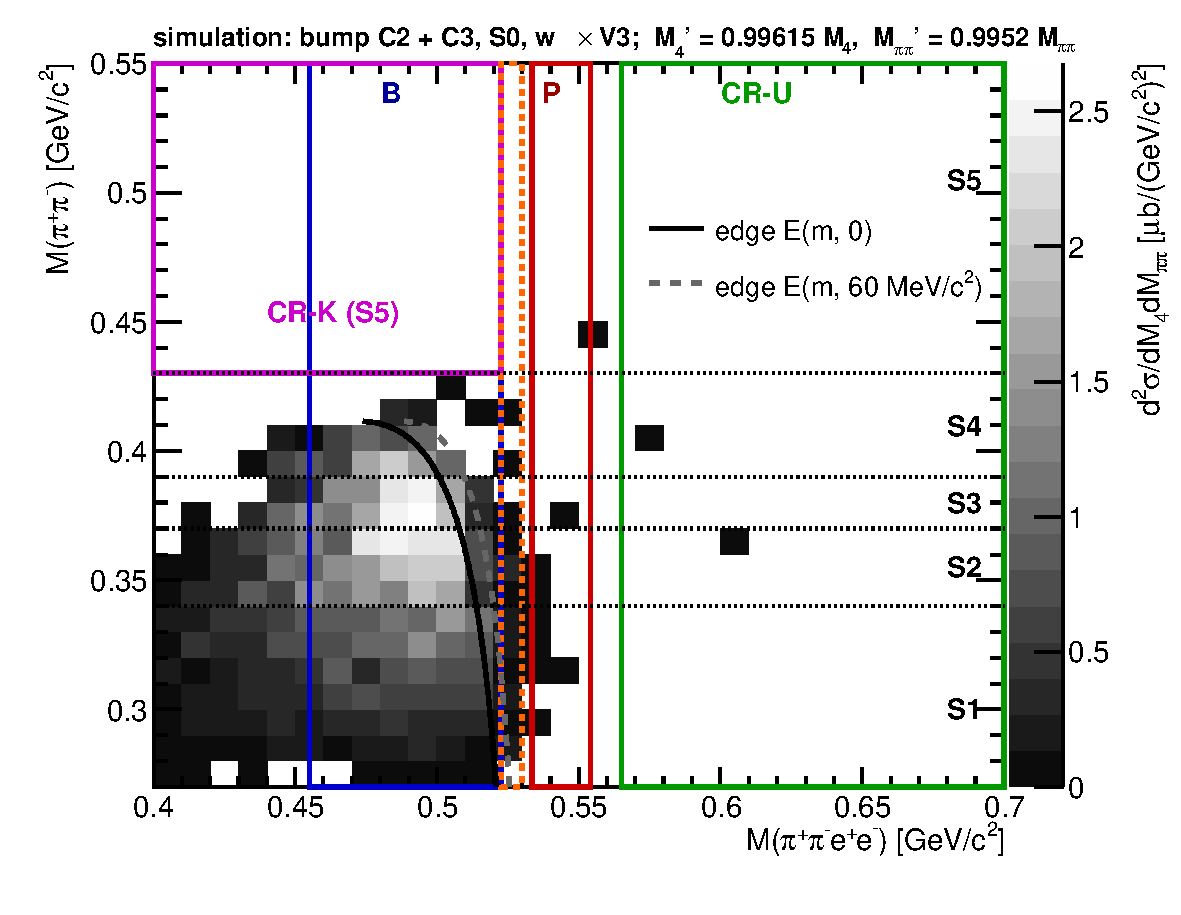
\includegraphics[width=0.72\textwidth]{figs_all/fix_definitions.pdf}
\caption{Definitions in the analysis plane \Mfour$\times$\Mpipi.
Selection: simulation only, the bump classes C2+C3 with the S0 cuts (PT3 trigger, event vertex at $\vz>-160$\,mm, \betanew identification (pions $3\sigma$, leptons $5\sigma$ with a RICH ring), corrected momenta, all stored combinations (isBest $\ge0$), both pions in the event-vertex fit), all \Mee; \Mfour 0.40--0.70\,\GeVcc $\times$ \Mpipi 0.27--0.55\,\GeVcc.
Grey scale: simulated bump C2+C3 (S0, SMASH mode A, $w\times$V3,
$M_4'=0.99615\,M_4$, $\Mpipi'=0.9952\,\Mpipi$; $\mu$b/(\GeVcc)$^2$, 10\,\MeVcc cells, $\Lsim=221.05\,\nbinv$; simulation only).
Dotted: slice boundaries 0.34, 0.37, 0.39, 0.43. Boxes: bump window B (blue), peak window P (red), CR-U (green), CR-K (magenta),
CR-L (orange, test only). Lines: $E(m,0)$ (solid) and $E(m,60\,\mathrm{MeV})$ (dashed). WP0 figure, title redrawn (\code{fix_wp0defs.C}).
No fall-back involved.}
\label{fig:defs}
\end{figure}

\subsection{The combinatorial background}
\label{sec:cb}
The CB is built from the like-sign \emph{data} counts only (D5):
\begin{enumerate}\setlength{\itemsep}{0pt}
\item $2\sqrt{N_{++}N_{--}}$ in 10\,\MeVcc cells of \Mfour from 0.30\,\GeVcc, linearly interpolated to 2.5\,\MeVcc bins (the rule of
      Part~II);
\item spread over the cells of a layout (slice, \Mee class) by the share $f(\mathrm{cell}\,|\,\mathrm{50\,MeV\ band})$ of the like-sign
      counts $N_{++}+N_{--}$ of that 50\,\MeVcc band (the ``spread rule'');
\item its error comes from 200 Poisson replicas: each like-sign event group gets a Poisson(1) weight, and steps 1--2 are repeated.
\end{enumerate}
Over whole windows the spread rule agrees with a per-cell geometric mean to 0.3\,\% (B 1.003, P 1.001, CR-U 1.003), but not in single
cells: the ratio per-cell geometric mean / spread rule is 0.64--0.91 in E1, 0.87--1.12 in E2, 0.65 in the X17 windows and 0.17 in CR-K
($N_{++}=2$). The reason is that $N_{--}/N_{++}$ is 7--18 at small \Mee and 3.6--6.3 at \Mee$\ge10$\,\MeVcc, while the rule uses one
like-sign share per band. The per-cell geometric mean is therefore a member of family S1. The replica error is 1.2--1.6 times the
linear propagation in E2 and 3.2--4.2 times in E1 (Fig.~\ref{fig:cberr}), because it includes the statistical error of the shares.
Stored CB errors without replicas (folds, periods, G3, the maps) are linear only and underestimate the error in E1 and CR-K by up to
a factor 2--4.

\begin{figure}[H]
\centering
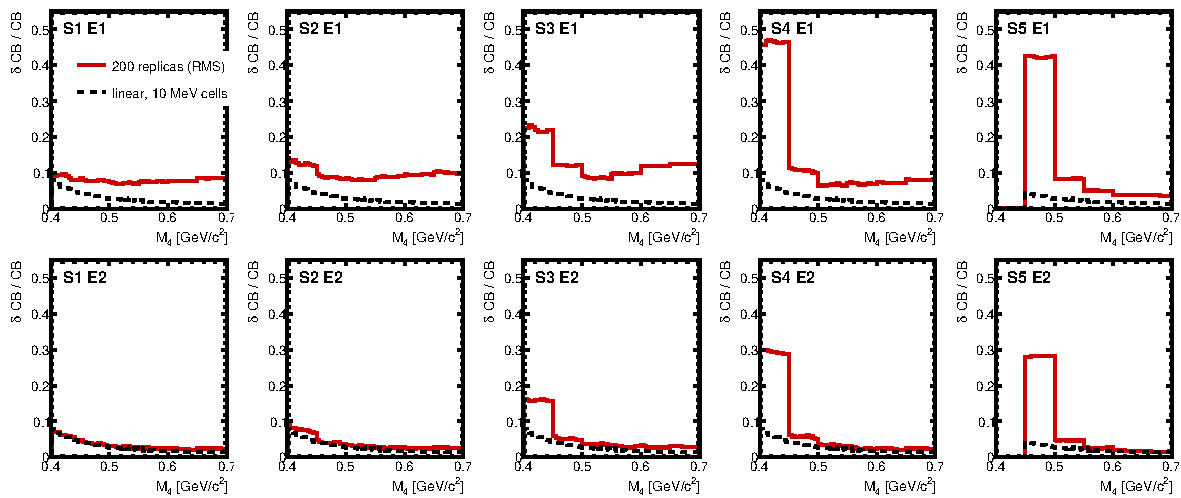
\includegraphics[width=\textwidth]{figs_all/wp0_cb_errors.pdf}
\caption{Relative uncertainty of the CB per F10 cell.
Selection: data S0 (PT3 trigger, event vertex at $\vz>-160$\,mm, \betanew identification (pions $3\sigma$, leptons $5\sigma$ with a RICH ring), corrected momenta, all stored combinations (isBest $\ge0$), both pions in the event-vertex fit); the ten F10 cells: five \Mpipi slices (below 0.34, 0.34--0.37, 0.37--0.39, 0.39--0.43, from 0.43\,\GeVcc) $\times$ \Mee below 10 (E1) and from 10\,\MeVcc (E2), \Mfour 0.400--0.700\,\GeVcc.
Data S0, raw counts, isBest $\ge0$. CB $=2\sqrt{N_{++}N_{--}}$ in 10\,\MeVcc
cells, spread by the like-sign share of the 50\,\MeVcc band. Red: rms of 200 Poisson event-group replicas of the like-sign counts.
Black dashed: linear propagation of the 10\,\MeVcc cell counts only. The difference is the statistical error of the cell shares;
it dominates in E1 and in S4/S5 below 0.50\,\GeVcc. No fall-back involved.}
\label{fig:cberr}
\end{figure}

\subsection{The model in plain words}
\label{sec:model}
All template fits of this report use one model for the number of counts $\mu$ expected in bin $i$ of histogram $h=(j,e)$
(slice $j$, \Mee class $e$):
\begin{align}
\mu_{hi}={}&k_e\,\mathrm{CB}_{hi}+c_j\,(1+b\,x_i)\,\big[G_D+\kappa_B\,G_C\big]_{hi}\nonumber\\
&+a_\eta\,\big[\mathrm{C2}+\kappa\,(\mathrm{C3}+\mathrm{C4})+\rho_d\,\mathrm{C5}+g\,G_\eta\big]_{hi},\qquad x=(\Mfour-0.55)/0.1.
\label{eq:model}
\end{align}
In words: the data are the like-sign CB (fixed shape, factor $k_e$), plus the SMASH non-$\eta$ background with a free scale per
\Mpipi slice and a common linear tilt in \Mfour (the conversion part $G_C$ may scale differently, \kB), plus all $\eta$ classes
of SMASH scaled by one common factor \aEta, with separate factors for the conversion classes ($\kappa$), the direct decay
(\rhod) and the other $\eta$ decays ($g$). The simulated templates are in expected raw counts (\S\ref{sec:simin}). The fits run on the raw
data counts; the yields are
\begin{equation}
Y_c=\tfrac{64}{63}\times(\text{fitted factor})\times\mathrm{C}c,\qquad Y_{\mathrm{bump}}=Y_2+Y_3\ \text{in B},\qquad Y_{\mathrm{peak}}=Y_4+Y_5\ \text{in P},
\label{eq:yields}
\end{equation}
\[
\mathrm{DR}=\frac{(Y_{\mathrm{peak}}/Y_{\mathrm{bump}})_{\mathrm{data}}}{(Y_{\mathrm{peak}}/Y_{\mathrm{bump}})_{\mathrm{sim}}}.
\]
The non-$\eta$ templates are smoothed (exp of a cubic polynomial in $x$ per histogram, integrated over each bin, the normalisation kept
exactly) because one simulated standard-set entry corresponds to about 27 expected data counts; the signal templates stay raw and their bin
variance enters the fit weights (``BB-lite'', D13). The statistical error of every fit is a sandwich error: the variance of the data
counts comes from the event groups and the CB variance from the 200 like-sign replicas. The template-statistics error (``MC'') is the
spread of 100 refits, each with one bootstrap replica of the simulation (every simulated event group gets a Poisson(1) weight).

\subsection{Corrections in plain words}
\label{sec:A2}
\phantomsection\label{tab:A2}
\textbf{Spec.\ Table~A2.} Corrections of this report: what each one does, its procedure, whether it is applied, and its size. The upper part
is WP1's table (\code{tables_all/wp1_A2.txt}, sizes measured on \code{hists_v1.root}) rewritten in the notation of the report, with the
pion-vertex efficiencies of WP8; the lower part adds the corrections used for the yields and the physics quantities (review fix,
\code{tables_all/fix_A2.tex}, with the event-vertex row of the final review in \code{fix2_A2.tex} and the rulings of 15 November 2026 (D21, D25, D26) in
\code{fix3_A2.tex}; sizes from the sections quoted).
\par
% fix3_A2_ra5.tex -- final check (2026-11-16): copy of fix3_A2_ra4.tex with "trigger word" -> "trigger bit" (analyst's PT3
% definition, P. Tlusty, 13 Dec 2024). Nothing else changed. Original header follows.
% fix3_A2_ra4.tex -- Part III long writer, fourth integration (2026-11-15): copy of fix3_A2.tex with "rows" -> "counts" (analyst instruction:
% a count is one stored pi+pi-e+e- combination). Original header follows.
% fix3_A2 (integration of 15 November 2026: rows C_sec, 1-f_eta, PDG edition updated; copy of fix2_A2.tex)
% fix2_A2.tex -- final review (prefix fix2, 2026-11-14): copy of fix_A2.tex with the event-vertex row replaced by the
% measurement (notes_all/ve_verify_note.md; tables_all/fix2_numbers.txt). Nothing else changed. Original header:
% fix_A2.tex -- review fix (prefix fix): Table A2 of WP1 (wp1_A2.tex) rewritten in LaTeX notation and completed with the
% corrections used later in the report (sizes from the results notes; nothing recomputed). Needs longtable, booktabs, array.
{\footnotesize\setlength{\tabcolsep}{3pt}
\begin{longtable}{>{\raggedright\arraybackslash}p{2.2cm}>{\raggedright\arraybackslash}p{3.6cm}>{\raggedright\arraybackslash}p{5.3cm}>{\raggedright\arraybackslash}p{1.25cm}>{\raggedright\arraybackslash}p{3.15cm}}
\toprule
correction & what it does & procedure & applied & size \\
\midrule
\endfirsthead
\toprule
correction & what it does & procedure & applied & size \\
\midrule
\endhead
\bottomrule
\endfoot
\multicolumn{5}{@{}l}{\emph{Corrections of the comparison (WP1)}} \\
Combinatorial background (CB) & Pairs of an $e^+$ and an $e^-$ that do not come from the same decay are removed by subtracting the like-sign pairs. & $\mathrm{CB}=2\sqrt{N_{++}N_{--}}$ from the $e^+e^+$ and $e^-e^-$ counts of the \emph{data} in 10\,\MeVcc \Mfour cells ($k=1$), linearly interpolated to 2.5\,\MeVcc and spread over the cells of a layout by the like-sign share of the 50\,\MeVcc band; error from 200 Poisson event-group replicas. The simulation never provides it. & yes (data) & CB$/N$: S0 B 0.056, P 0.059; ``pre'' B 0.101, P 0.103 \\
Luminosity and trigger bit ($64/63$) & Turns counts into cross sections. & $\sigma=(N-\mathrm{CB})\times\frac{64}{63}/L$, $L=6079.2\,\nbinv$: elastic luminosity of the 17\,557 analysed runs (START-free chain, LH$_2$ only, sector-2 PT2 deficit removed inside $L$). $64/63$: 1/64 of the PT3 events carry trigger bit 4096, FAT keeps bit 8192. & yes & $\times1.01587/L$ ($\pm6.9$\,\%); old tables (6080.5, no $64/63$) $\times1.0161$ \\
Live time of the PT3 input & The PT3 live fraction may be lower than the PT2 one contained in $L$. & LF3/LF2 $\times64/63$ per day from the luminosity files (0.900--0.948, $L$-weighted 0.932--0.933). Unknown whether it applies to single-interaction PT3 events. & no & one-sided $+7.1$ to $+7.3$\,\% on cross sections \\
Mass scale of the simulation (D8) & The simulated $\eta$ peak sits at 0.5460\,\GeVcc, the data peak at 0.5439; the simulated \Mfour is moved onto the data scale. & $M_4'=s\,[m_4^{\mathrm{true}}+r_{\mathrm{res}}(m_4-m_4^{\mathrm{true}})]$, $s=0.99615$, $r_{\mathrm{res}}=1$ (simulated entries without a true mass: $s\,m_4$); \Mpipi$\times0.9952$ from the K$^0_S$ position; \Mee not scaled. Variants $s=0.99521$, $0.99615\pm0.0009$, $r_{\mathrm{res}}=0.89/1.10$. & yes (sim) & ``pre'' data/sim against unscaled: B $-0.96$\,\%, P $-1.73$\,\%, $J$ $-2.5$\,\%; C5 in P at $r_{\mathrm{res}}=0.89/1.10$: $\times1.043/\times0.960$ \\
$\eta$ decay physics weights V3 (code 108) & The generator decays $\eta\to\ppee$, the $\eta\to3\pi$ Dalitz plot and the conversion photon spectrum without the measured matrix elements; a weight per simulated entry corrects this. & Direct decay: Kroll--Wada $\times$ pion P-wave $\times|F_V|^2\times|F_{\mathrm{VMD}}|^2\times$ decay angles, divided by the generator density (mean weight 1, BR unchanged); bump: KLOE-2 Dalitz-plot parameters; conversion: $|F_V|^2$ photon spectrum; background rules. & yes (sim) & S0: $T_{12}$ in B $\times0.971$, in P $\times1.020$; C2+C3 in B $\times0.937$; C4 in P $\times1.063$; C5 in P $\times1.038$ \\
Beam energy & Data analysed at $T=4530$\,MeV, simulation generated at 4500\,MeV. & \MMfour and $y_4$ are recomputed for every simulated entry at 4500\,MeV and for the data at 4530\,MeV; \Mfour, \Mpipi, \Mee, OA do not depend on it. SMASH cross sections are those at 4.5\,GeV. & yes (\MMfour, $y_4$) & \MMfour and $y_4$ spectra differ by the beam energy \\
Pions in the vertex fit (S0) & S0 keeps only combinations whose two pion tracks were used in the event-vertex fit; the simulation must reproduce how often this happens. & S0/``pre'' of the $\eta$ peak and of the ECAL-tagged $\eta$ in data against simulation (WP8): peak $0.941\pm0.052$ vs 0.940, tagged $0.933\pm0.013$ vs 0.933. Not applied; it cancels in ratios. & no (S12, $\pm2.5$\,\%) & data/sim $1.002\pm0.056$ (peak), $1.000\pm0.014$ (tagged) \\
Corrected momenta (\code{cor_ok}) & The energy-loss corrected \pim momentum is missing for \pim at $\theta<16^\circ$ (0.62\,\% of the \ee combinations). & Combinations with \code{cor_ok} $=0$ are dropped in the data; the simulation has none. Fall-back (data only, test): the reconstructed \pim momentum. & yes & fall-back/nominal: B 1.014, P 1.013; on \Ypeak $+2.2\pm1.0$\,\% (one-sided, not applied) \\
Ghost tracks (variant (a)) & PAT marks some simulated lepton tracks as ghosts. A true one-source \ee pair with such a track counts as signal ($T_1$) in an $\eta$ channel but as a fake lepton ($T_3$) when it is background; the like-sign data do not contain these pairs, the data $N-\mathrm{CB}$ does. & Variant (a) moves the ghost-flagged true pairs from $T_3$ into $T_2$, so that signal and background are treated alike. Systematic (S4); the ruling is pending (D6). & variant & simulation $T_{12}$(a)$/T_{12}$: B 1.092, P 1.116, all \Mfour 1.162; the data/sim ratios fall by 8.5--14.5\,\% \\
Ownership and branching ratios & The three simulated sets describe the same SMASH events; each simulated entry is counted once, with the PDG branching ratio. & Mode A: the lepton set owns entries with a forced \piz/$\eta$/$\rho$/$\omega$/$\phi$ product, the $\eta$ set entries with a forced-$\eta$ track; weight $w$ $=$ PDG BR (PDG 2020) correction. Variants: mode B, $w_{\mathrm{db}}$. & yes (sim) & $T_{12}$ all \Mfour: mode B $\times1.055$, $w_{\mathrm{db}}$ $\times1.024$ \\
Vertex cut $\vz>-160$\,mm & Removes interactions outside the LH$_2$ cell; the simulation has almost no entries there. & Applied to data and simulation alike ($\vz>-500$\,mm is mandatory anyway). Below $-160$\,mm lie 7\,\% of the data counts and 0.15\,\% of the simulated entries. Variants $-150$/$-170$\,mm (S11). & yes (both) & data ``pre''/none: $N$ in B 0.897, P 0.901; $N-\mathrm{CB}$ B 0.930, P 0.933 \\
\midrule
\multicolumn{5}{@{}l}{\emph{Corrections of the yields and of the physics quantities (WP2, WP6, WP8, verifications)}} \\
Sector-2 PT3 deficit, \Csec & Days 034--045 lack PT3 triggers with a sector-2 track; $L$ does not contain this. & Double ratio of counts with/without a sector-2 track, deficit/clean days: $\varepsilon_{s2}=0.9266\pm0.0024$; simulated share $f_s$ of the signal with a sector-2 track; $\Csec=1/[1-f_s(1-\varepsilon_{s2})L_{034-045}/L]$ (\S\ref{sec:norm}). Span 034--045 approved by the analyst on 15 November 2026 (D26); the elastic events (PT2, PT3) show no sector-2 deficit on day 045, so $L$ needs no correction there. & yes ($\eta$ yields) & 1.0104 (bump), 1.0116 (peak) \\
Target material of the $\eta$, $1-\feta$ & Removes $\eta$ mesons produced in the target windows (L counts LH$_2$ only). & Amendment~1 (D21, approved by the analyst on 15 November 2026): $\feta=3^{+4}_{-3}$\,\% from the vertex slices and the cell-centre share of $S$ and $T$; \fwin (13--15\,\% of $N-\mathrm{CB}$) describes only the non-$\eta$ background and is \emph{not} applied to $\eta$ yields (\S\ref{sec:norm}). & yes ($\eta$ yields) & $\Csec(1-\feta)=0.98^{+0.03}_{-0.04}$ \\
Event-vertex efficiency of $\vz>-500$\,mm & Removes the combinations without an event vertex (32\,\% of the \ee counts; 0.565 survive in P), mostly non-target (probably upstream) events. & $\varepsilon_{\mathrm{vtx}}(\eta)=X_V/(X_V+X_{Nv})$ measured in the data for $S$ (smooth like-sign CB), $T$ and $E$, combined: $0.994\pm0.021$ ($0.990\pm0.022$ with the nominal CB); simulation 0.9997 (\S\ref{sec:vertexeff}). & no & $C_{\mathrm{vtx}}=1.006\pm0.021$, one-sided $+2$\,\% ($+4$\,\% at 95\,\% CL) \\
Side-band leakage $1/(1-R'f)$ & The $\eta$ peak leaks into its own side bands; subtracting them removes part of the signal. & Closed form of the iteration $Y_{n+1}=(N-\mathrm{CB})_{\mathrm{P}}-R'[(N-\mathrm{CB})_{\mathrm{SB}}-fY_n]$ with $f=0.1544$ from the simulated C4+C5 shape and $R'=1.1859$ (\S\ref{sec:sb}). & yes (\Ypeak) & $+22$\,\% (4156 $\to$ 5088 counts) \\
$\eta$ content of the upper region, $\eta_{\mathrm{U}}$ (B4) & The region U used to normalise the bump background holds $\eta$ counts (mostly \Geta). & $\eta_{\mathrm{U}}$ at the F-main values (14\,399 counts) is subtracted from $(N-\mathrm{CB})_{\mathrm{U}}$ before the transfer into B (WP4/WP6 implementation; \S\ref{sec:b4}). & yes (B4) & without it B4(E2) $-24$\,\% \\
Bump: E2 $\to$ all \Mee, $f_{E2}$ & B4 exists only in E2 ($\Mee\ge10$\,\MeVcc); the all-\Mee yield needs the E1 share. & $\Ybump(\mathrm{all})=\Ybump(E2)/f_{E2}$, $f_{E2}=(\mathrm{C2}+\kappa\mathrm{C3})_{E2}/(\mathrm{C2}+\kappa\mathrm{C3})_{\mathrm{all}}=0.4773$ at $\kappa=0.832$ (0.4448--0.5203 for $\kappa\pm1\sigma$). & yes (B4 all) & $\times2.095$; $+1196/-1356$ counts \\
PDG edition & The simulation uses the PDG 2020 branching ratios; PDG 2026 differs. & Rescaling of the simulated classes: C2, C3 $\times1.00436$, C4 $\times1.01422$, C5 $\times1.02985$ (verifier v8). The X17 limit is quoted with PDG 2026, BR$_{\mathrm{dir}}=2.76\times10^{-4}$ (D25, ruled by the analyst on 15 November 2026); the frozen procedure used $2.68\times10^{-4}$. & yes (P2) & \sigeta $-2.19$\,\%; \BRG, \BRA $+0.4$\,\%; DR $-1.8$\,\%; X17 UL $3.06\to3.16\times10^{-5}$ ($\times1.031$) \\
SMASH $\sigma(\eta)$ & The simulated sample has 1.0694\,mb, not the 1.0665\,mb of a sub-sample. & $N_\eta=2.364\times10^8$ in $10^{10}$ events (v8). & yes & \sigeta $+0.28$\,\% \\
Composition of the peak & $\aP=\Ypeak/(\mathrm{C4}+\mathrm{C5})_{\mathrm{SMASH}}$ is the $\eta$ scale only if SMASH has the right conversion/direct mix (C4 is 47\,\% of the simulated peak). & The data favour a direct/conversion mix 2--2.7 times SMASH's (\S\ref{sec:p2}); half the difference of the direct-decay and conversion routes is the systematic. & syst only & \sigeta $\pm31.8$\,\% \\
\end{longtable}}


\subsection{Histogram factory and its checks}
\label{sec:factory}
One pass over the data and the simulation (WP0, \code{wp0_fill.C}, 157\,s, 7.4\,GB) fills every histogram of this report into
\fpath{/hdd3/przygoda/HADES/FAT_out/all_report/hists_v1.root} (write-protected): 11 data selections $\times$ 7 subsets (all, two
folds, four periods) with $N$, $N_{++}$, $N_{--}$, CB and the CB replicas; 34 simulation directories (S0 and ``pre'' with 15 variants
each, and dz40, PEAK, vz150, vz170 nominal) with 22 components, two halves (even/odd event group) and 100 bootstrap replicas.
Table~\ref{tab:wp0acc} gives the acceptance criteria.

\begin{table}[H]
\centering
\caption{Acceptance criteria of the histogram factory (WP0). All four pass; the verifier v0 recomputed 189 quantities with its own
code (no shared headers) and found all equal (counts exactly, CB and simulation to $10^{-9}$). No fall-back involved.}
\label{tab:wp0acc}
\small
\tabin{wp0_acceptance.tex}
\end{table}

The simulated cross sections of every variant directory are listed in Table~\ref{tab:simtot} (Appendix~\ref{app:norm}). Further checks:
the simulation replicas have an rms equal to the event-group error (ratio 0.989--1.016, median per histogram); the two halves differ
as expected from their effective statistics (0.954--1.065); the effective number of simulated entries per F10 histogram is
1\,782 (S3E1) to 7\,141 (S1E2) for $T_1+T_2$.

\subsection{Blinding}
\label{sec:blind}
Before any X17 fit (D19): the data $N$ of X2D with \Mee 12--28\,\MeVcc (all \Mfour bins) and of the \Mee distributions of the regions
R2--R4 in 12--28\,\MeVcc were set to $-1$ in \code{hists_v1.root}; the unmasked cells were written only to a sealed file, which was
opened for the first time after \code{x17_frozen.txt} (procedure, priors and expected limit) existed. $N_{++}$, $N_{--}$ and the CB
were not masked. Known before the freeze, and stated here: the counts 5258 (X17P) and 6424 (X17c, CB 209.5; with the rounded edges 0.5312--0.5566;
Part~II quotes $N=6395$ for the same window because it uses the exact edges 0.531249--0.556551, the simulation window $\times0.5439/0.5460$:
29 counts fewer, checked with \code{fix2_x17count.C}), and the peak share above
20\,\MeVcc. The CB of the 5258 X17P counts has three values: 112 (D19: $2\sqrt{N_{++}N_{--}}$ of the whole window, $N_{++}=14$,
$N_{--}=223$), $171\pm6$ (the spread rule of this report) and 101.7 (Part~II, Table res\_x17: the rule of Part~II, 10\,\MeVcc \Mfour cells of
the band's own like-sign counts, interpolated; about $\pm14$ from the Poisson errors of $N_{++}$ and $N_{--}$). Coarse \Mee information remained
unmasked (F10 E2, F5g, the G3 classes 12--20 and $\ge20$\,\MeVcc, and the OA distributions in 1$^\circ$ bins); the verifier v0 noted
that these hold X17-sensitive information in principle, and every package declared that it did not form them in the peak band. One
cell of a test file (8 entries, built from the first 200\,000 entries) was opened once during development to check the copy.

\textbf{Not blind in the information.} Part~II (\code{report_exp.pdf}, \S7.7 ``A look at the X17 band'', Table res\_x17 and Fig.\ res\_x17\_window;
\S6.8) showed the side-band-subtracted \Mee spectrum of the $\eta$-peak counts (S0, data peak window) in 3\,\MeVcc bins across 13--27\,\MeVcc and
the 9\,\MeVcc band 15.5--24.5\,\MeVcc: $D=481\pm99$ $\eta$-peak counts against $522\pm111$ interpolated from the neighbouring bands
(difference $-40\pm149$), and the \Pmain content of the band $S=440\pm92\pm60$. These numbers were in the Part~II results note (05:11) and in
\code{report_exp} (06:30--06:49), before the freeze (\code{x17_frozen.txt}, 07:54). The notes of the X17 packages (x17ab, x17c) do not cite
Part~II or these numbers; whether the X17 agents read them cannot be established from the records. The search is therefore \textbf{blind in
the code, not in the information}: the procedure was frozen without opening the masked cells, but the \Mee shape of the peak band was
public (it showed no excess). An influence of this knowledge on the frozen choices cannot be excluded; the choices are documented with
their reasons (side-band fit, toys) in \S\ref{sec:x17}.

%======================================================================
\section{How SMASH describes the data before any renormalisation}
\label{sec:before}
%======================================================================
\inshort{without any adjustment data/SMASH lies between 0.74 and 1.27 and changes with \Mfour: 0.86 in the bump window, 1.10 in the peak window, 1.27 just above the peak and 0.74 at 0.90--1.10\,\GeVcc; one common scale leaves $\chi^2/\mathrm{ndf}=12$. SMASH does not describe the shape. The data hold about 0.3 of the SMASH K$^0_S$.}
\textbf{Procedure} (WP1, \code{wp1_before.C}, \code{wp1_repro.C}).
\begin{enumerate}\setlength{\itemsep}{0pt}
\item The data are converted to cross sections, $(N-\mathrm{CB})\times64/63/L$, with the CB from the like-sign data ($k=1$, spread
      rule). Data errors: event groups, plus the rms of the 200 CB replicas where they exist (windows, 1D spectra, F10 cells).
\item The simulation is the sum $T_1+T_2$ of SMASH (std + lep + $\eta$, mode A, $w\times$V3), every channel at its own SMASH
      production cross section $\times$ PDG BR $\times$ weight; $\sigma=\sum w/221.05\,\nbinv$; mass transfer of D8. Nothing is
      renormalised.
\item The 6.9\,\% of $L$ is not in the quoted errors; it is drawn as a band in the ratio panels. The live time ($+7.3/-0$\,\%) is not
      applied and is drawn as a separate hatched band.
\item Ratios data/simulation are formed per \Mfour region (Table~\ref{tab:B1}), together with the jump
      $J=R(0.560$--$0.595)/R(0.4875$--$0.5225)$ and a shape test with one free scale $a$ (data $=a\times$ simulation) in 0.40--0.70.
\end{enumerate}

\begin{table}[H]
\centering
\caption{Spec.\ Table~B1: data/simulation per \Mfour region before any renormalisation. Data $(N-\mathrm{CB})\times64/63/L$, $L=6079.2\,\nbinv$;
simulation SMASH $T_1+T_2$, mode A, $w\times$V3, $M_4'=0.99615\,M_4$. Column (a): ghost variant (a). Last two columns: the ratio of the
data contents isBest $=1$ / isBest $\ge0$ of the same selection (D2, data only, errors in the last digits in brackets). Errors: data
statistics $\oplus$ MC statistics; the 6.9\,\% of $L$ is common and not included. Window contents are $N-\mathrm{CB}$ with all background,
not signal yields (D20). Source: WP1, \code{tables_all/wp1_B1.txt}. No fall-back involved.}
\label{tab:B1}
\small
\tabin{wp1_B1.tex}
\end{table}

\begin{figure}[H]
\centering
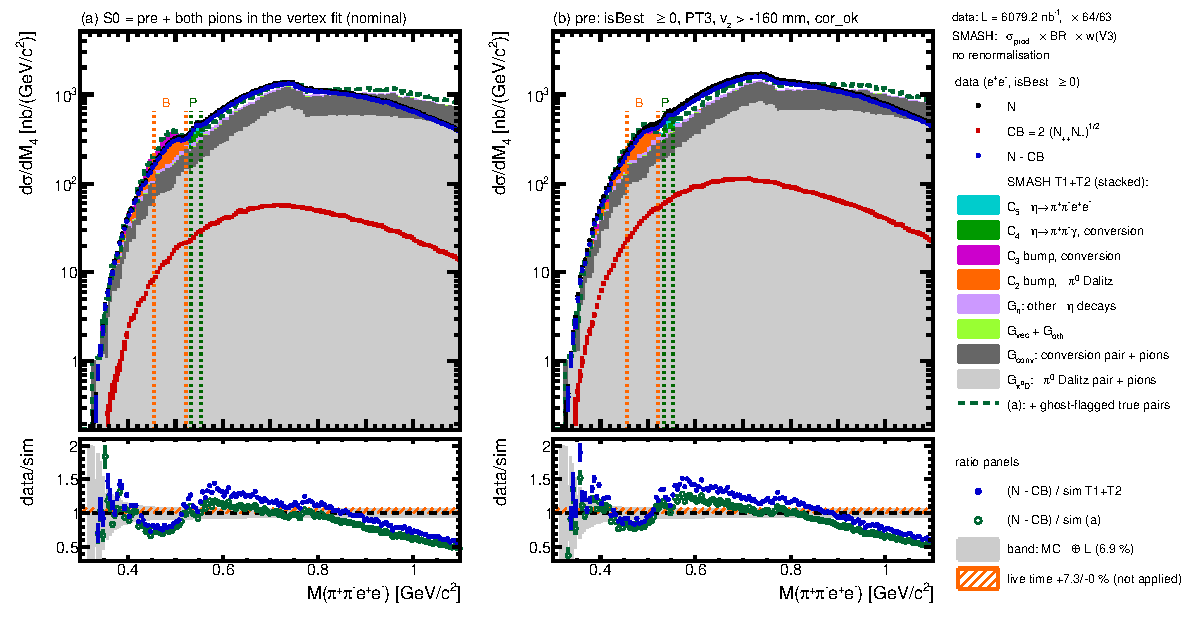
\includegraphics[width=\textwidth]{figs_all/fix_B1.pdf}
\caption{Spec.\ Fig.~B1: \Mfour from 0.30 to 1.10\,\GeVcc (5\,\MeVcc bins, log scale) before any renormalisation.
Selection: (a) data S0 (PT3 trigger, event vertex at $\vz>-160$\,mm, \betanew identification (pions $3\sigma$, leptons $5\sigma$ with a RICH ring), corrected momenta, all stored combinations (isBest $\ge0$), both pions in the event-vertex fit); (b) ``pre'' (the same without the pion-vertex condition); all \Mpipi and \Mee; SMASH $T_1+T_2$ with the same cuts, nothing renormalised.
(a) S0 (nominal); (b) ``pre'';
same $y$ range. Data (isBest $\ge0$): $N$ black, CB $=2\sqrt{N_{++}N_{--}}$ from like-sign data red ($k=1$), $N-\mathrm{CB}$ blue, as
$d\sigma/dM_4$ with $\times64/63$ and $L=6079.2\,\nbinv$. Stacked: SMASH $T_1+T_2$ by group at $\sigma_{\mathrm{prod}}\times$PDG BR$\times$V3,
$\Lsim=221.05\,\nbinv$, $M_4'=0.99615\,M_4$; dashed: ghost variant (a). Dotted: windows B and P. Lower panels: $(N-\mathrm{CB})$/simulation
(full) and /variant (a) (open); grey band MC $\oplus$ 6.9\,\% luminosity; hatched: possible live-time correction $+7.3/-0$\,\% (not
applied). The mandatory cut $\vz>-500$\,mm keeps $0.994\pm0.021$ of the target $\eta$ in the data and 0.9997 in SMASH
(\S\ref{sec:vertexeff}): the ratios need no vertex correction. WP1 figure redrawn with the CB legend written as
$2(N_{++}N_{--})^{1/2}$ (\code{fix_wp1.C}). No fall-back used.}
\label{fig:B1}
\end{figure}

\begin{figure}[!htbp]
\centering
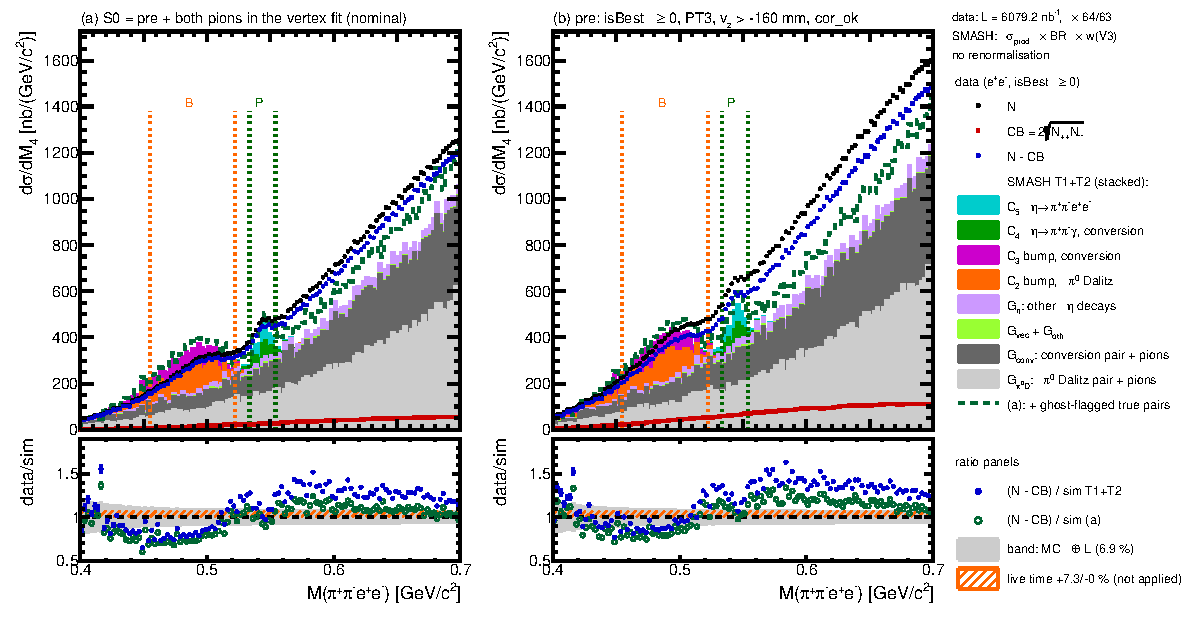
\includegraphics[width=\textwidth]{figs_all/wp1_B2.pdf}
\caption{Spec.\ Fig.~B2: the same as Fig.~\ref{fig:B1} in 0.40--0.70\,\GeVcc, 2.5\,\MeVcc bins, linear scale.
Selection: (a) data S0 (PT3 trigger, event vertex at $\vz>-160$\,mm, \betanew identification (pions $3\sigma$, leptons $5\sigma$ with a RICH ring), corrected momenta, all stored combinations (isBest $\ge0$), both pions in the event-vertex fit); (b) ``pre'' (the same without the pion-vertex condition); all \Mpipi and \Mee; SMASH $T_1+T_2$ with the same cuts, nothing renormalised.
(a) S0, (b) ``pre'';
normalisation, colours and bands as in Fig.~\ref{fig:B1}. No fall-back involved.}
\label{fig:B2}
\end{figure}

\textbf{What the ratios say} (S0, Table~\ref{tab:B1}):
\begin{itemize}\setlength{\itemsep}{0pt}
\item Data/simulation rises from $0.861\pm0.013$ in the bump window B to $1.266\pm0.008$ in 0.565--0.70 and falls to $0.744\pm0.003$ in
      0.90--1.10. One free scale over 0.40--0.70 leaves $\chi^2/\mathrm{ndf}=723.7/59=12.3$ (1D, $a=1.191\pm0.006$) and 2.55 on the 656 used
      F10 cells (the cells have larger errors; the description is not better). ``pre'' behaves the same (13.0 and 3.08).
\item In the peak window P the ratio is $1.101\pm0.022$ (``pre'' $1.212\pm0.022$); the jump is $J=1.467\pm0.036$ (``pre'' $1.431\pm0.032$).
\item In the bump window the bump classes C2+C3 are 9.01\,nb of the simulated 20.38\,nb (44\,\%), $G_{\pi^0D}+G_{\mathrm{conv}}$ 10.14 and
      \Geta 0.97\,nb; in P the peak classes C4+C5 are 2.00\,nb of 8.00\,nb (25\,\%), \Geta 0.61 and $G_{\pi^0D}+G_{\mathrm{conv}}$ 5.27\,nb.
      Both windows are dominated by the background (56\,\% and 75\,\% of the simulated content), so their ratios mix the $\eta$ scale with
      the background scale; the renormalisation of \S\ref{sec:cr} separates the two.
\item The ghost variant (a) raises the simulation by 9--17\,\% and lowers the ratios by 8.5--14.5\,\% per region (Table~\ref{tab:B1}):
      the 0.40--0.70 scale goes from 1.19 to 1.03 and $J$ from 1.47 to 1.37 ($-6.6$\,\%) (D6, ruling pending).
\item About 13--15\,\% of the data $N-\mathrm{CB}$ in 0.40--0.70 comes from the target material (empty-target measurement,
      \S\ref{sec:norm}); SMASH does not simulate it. Part of the excess of the data over SMASH above the peak is this material.
\item \textbf{The event-vertex cut and these ratios} (measured after the first version of this report, \S\ref{sec:vertexeff}). The
      mandatory cut $\vz>-500$\,mm keeps 0.565 of the unlike-sign data counts in P (0.677 of all unlike-sign counts). The removed counts are mostly
      not LH$_2$ events (87\,\% of their pion pairs cross 8\,mm or more from the beam axis, against 35\,\% with a vertex; their pp-elastic content
      is 0.028 of the cell's), and SMASH does not simulate them. The ratios of this section (0.86 / 1.27 / 0.74, ``SMASH short of \ee pairs'')
      concern all $N-\mathrm{CB}$, mostly non-$\eta$ background, so the $\eta$ efficiency ($0.994\pm0.021$ in the data, 0.9997 in SMASH) does not
      by itself cover them. What covers them is that target events of any kind keep their vertex: (i) when the two pions cross inside the cell
      ($-170\le z<-85$\,mm, $r<8$\,mm), only 0.15\,\% of the combinations lack a vertex (3339 of 2.19 million, \code{ve_data_note.md}); (ii) resolution
      estimate: 2.19\,\% of the data combinations of target events have at most one own track in the finder window (simulation 0.09\,\%), and such a combination
      loses its vertex with probability 0.33--0.38 in the simulation (other tracks of the event rescue the rest), so the data lose at most about
      0.8\,\% of the target combinations (simulation 0.03\,\%; an upper estimate, \code{ve_sim_cause_note.md}). These ratios therefore need no vertex
      correction at the 1\,\% level. The K$^0_S$ is the exception (below).
\end{itemize}

\begin{figure}[H]
\centering
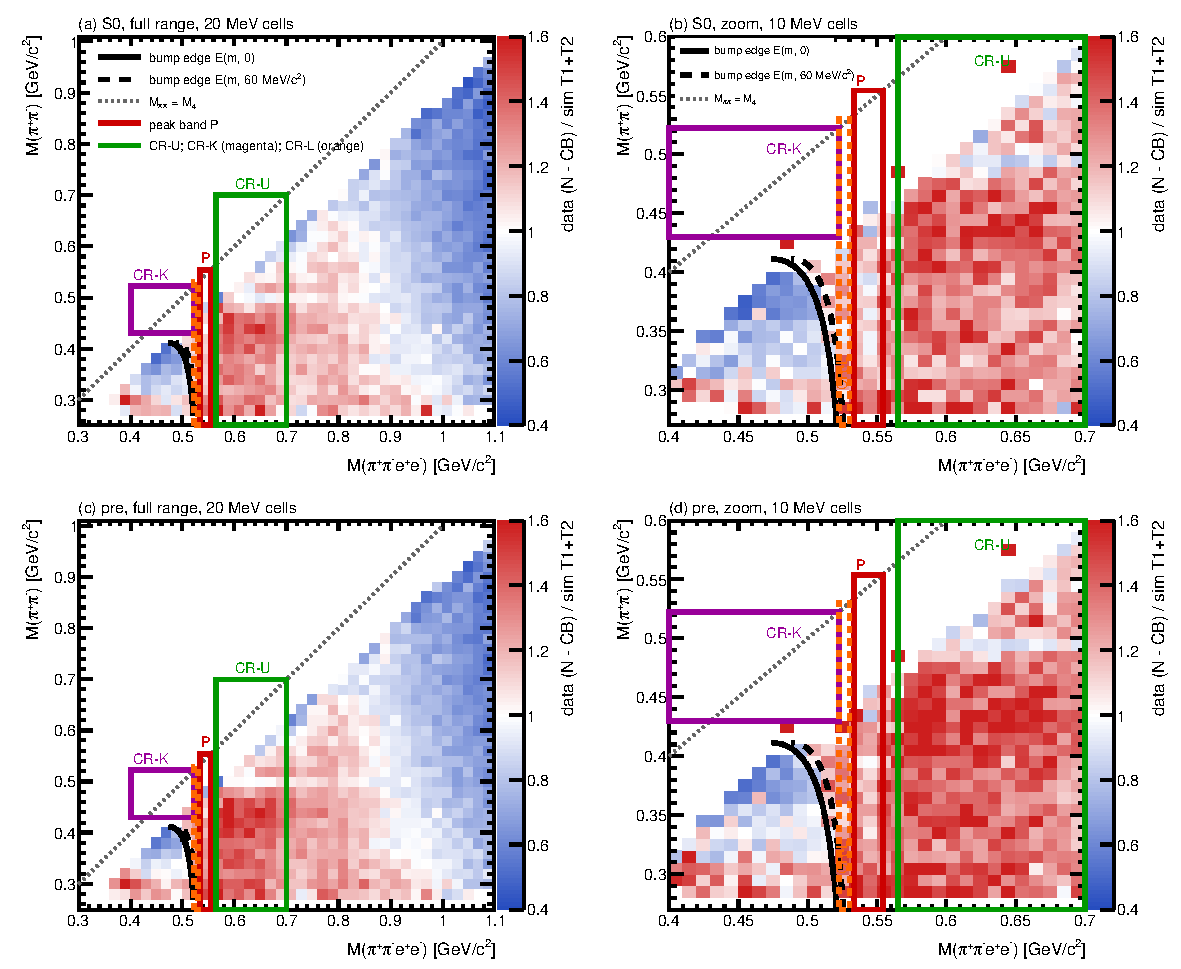
\includegraphics[width=0.88\textwidth]{figs_all/fix_B3.pdf}
\caption{Spec.\ Fig.~B3: ratio data $(N-\mathrm{CB})$ / simulation ($T_1+T_2$) in the plane \Mfour$\times$\Mpipi.
Selection: (a, b) data S0 (PT3 trigger, event vertex at $\vz>-160$\,mm, \betanew identification (pions $3\sigma$, leptons $5\sigma$ with a RICH ring), corrected momenta, all stored combinations (isBest $\ge0$), both pions in the event-vertex fit); (c, d) ``pre'' (the same without the pion-vertex condition); all \Mee; (a, c) \Mfour 0.30--1.10\,\GeVcc $\times$ \Mpipi 0.25--1.00\,\GeVcc, (b, d) \Mfour 0.40--0.70\,\GeVcc $\times$ \Mpipi 0.27--0.60\,\GeVcc; SMASH $T_1+T_2$ with the same cuts.
(a, b) S0; (c, d) ``pre'';
(a, c) full range in 20\,\MeVcc cells, (b, d) zoom 0.40--0.70 in 10\,\MeVcc cells. A cell is shown if its relative error is below 20\,\%
and $N-\mathrm{CB}>0$; colour scale clipped to 0.4--1.6. Lines: $E(m,0)$ (solid), $E(m,60\,\mathrm{MeV}/c^2)$ (dashed), \Mpipi$=$\Mfour
(dotted, kinematic limit). Boxes in the common colours: P (red), CR-U (green), CR-K (magenta), CR-L (orange, test only). Normalisation as
in Fig.~\ref{fig:B1}; CB errors of the map are linear (no replicas). WP1 figure redrawn with these box colours (\code{fix_wp1.C}). No
fall-back used.}
\label{fig:B3}
\end{figure}

The map (Fig.~\ref{fig:B3}) shows that the excess above the peak sits at all \Mpipi below 0.5\,\GeVcc. Below the bump edge the
ratio is 0.6--1.0 at \Mpipi 0.33--0.40 and above 1 at \Mpipi$<0.32$\,\GeVcc: the bump region is \Mpipi-dependent before any fit,
which is why the fits use five slices.

\textbf{Other variables.} Fig.~\ref{fig:B4} shows \Mpipi and \Mee in the regions R0--R7; the distributions of OA, \vz, \MMfour,
$p_{T,4}$ and $y_4$ are in Appendix~\ref{app:figs}, and the same figures for ``pre'' are in \code{figs_all/wp1_B4_<var>_pre.pdf}.
Main observations: above the \piz mass (\Mee$>0.14$\,\GeVcc) data/simulation is 1.5--2 in every region, i.e.\ SMASH is short of the
\ee continuum there; at small \Mee in R6--R7 it is 0.5--0.8. \MMfour and $y_4$ are computed at 4530\,MeV for the data and at
4500\,MeV for the simulation, so their ratios contain the beam-energy difference. In R2--R4 the data \Mee in 12--28\,\MeVcc and the
data OA in 4--30$^\circ$ are not drawn (blinding; the OA mask was added by WP1).

\begin{figure}[!htbp]
\centering
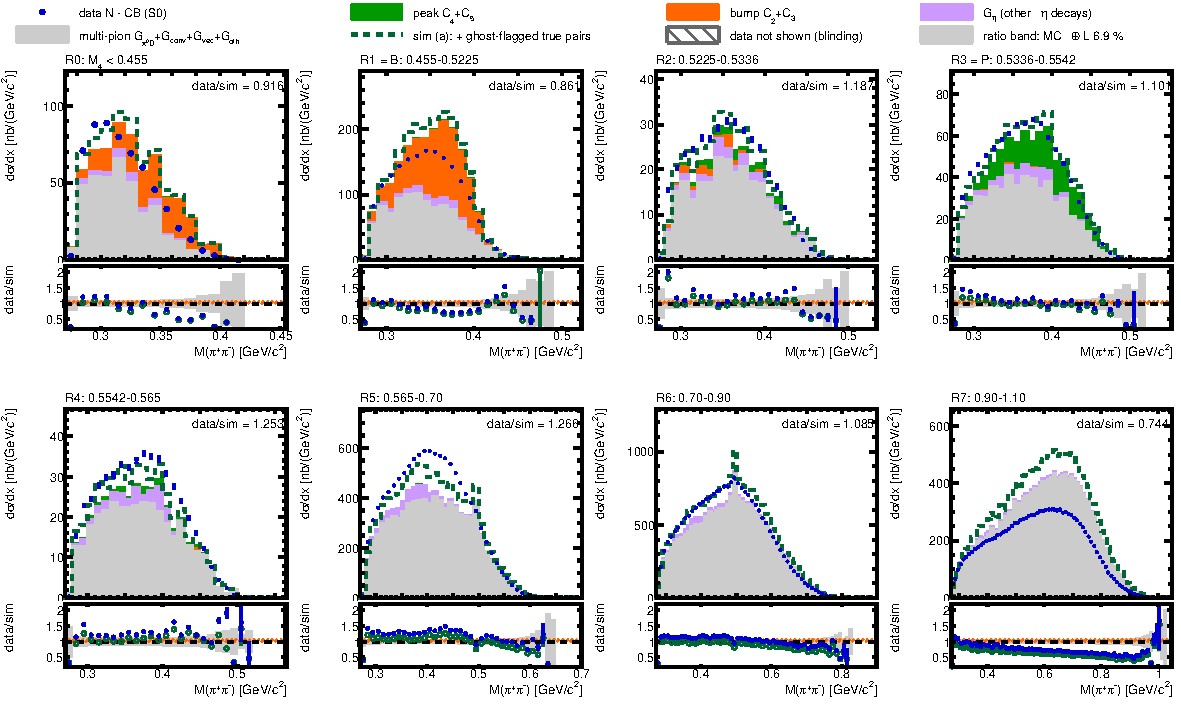
\includegraphics[width=\textwidth]{figs_all/wp1_B4_mpipi.pdf}\\[0.3em]
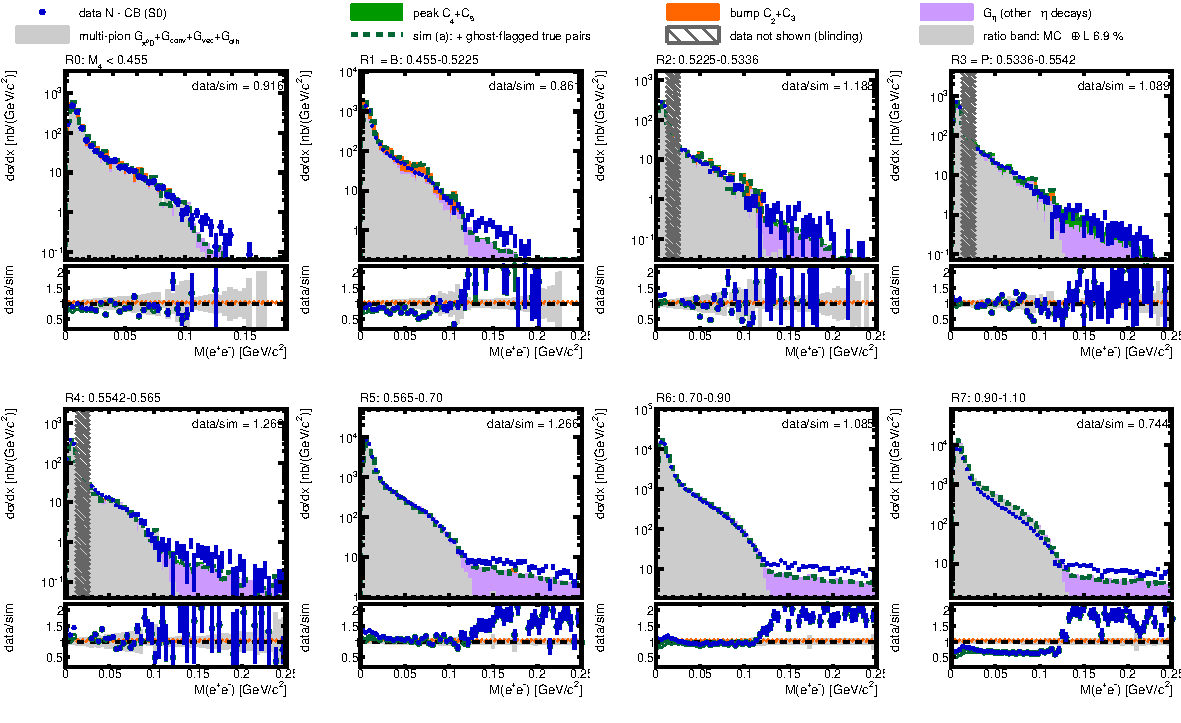
\includegraphics[width=\textwidth]{figs_all/wp1_B4_mee.pdf}
\caption{Spec.\ Fig.~B4: \Mpipi (top) and \Mee (bottom) in the eight \Mfour regions R0--R7 of Table~\ref{tab:B1}, selection S0.
Selection: data S0 (PT3 trigger, event vertex at $\vz>-160$\,mm, \betanew identification (pions $3\sigma$, leptons $5\sigma$ with a RICH ring), corrected momenta, all stored combinations (isBest $\ge0$), both pions in the event-vertex fit) and SMASH $T_1+T_2$ with the same cuts, in the \Mfour regions R0--R7 (below 0.455, 0.4550--0.5225, 0.5225--0.5336, 0.5336--0.5542, 0.5542--0.565, 0.565--0.70, 0.70--0.90, 0.90--1.10\,\GeVcc).
Blue: data
$N-\mathrm{CB}$, with CB $=$ CB(region) $\times$ like-sign share of the bin. Stacked simulation: multi-pion ($G_{\pi^0D}+G_{\mathrm{conv}}
+G_{\mathrm{vec}}+G_{\mathrm{oth}}$), \Geta, bump C2+C3, peak C4+C5; dashed: variant (a). ``data/sim'' in each panel is the region integral.
Each region has its own $y$ range. In R2--R4 the data at \Mee 12--28\,\MeVcc are masked (hatched, D19). CB errors linear only.
Normalisation as in Fig.~\ref{fig:B1}. No fall-back involved.}
\label{fig:B4}
\end{figure}

\textbf{The K$^0_S$ peak} (Fig.~\ref{fig:K0S}). A Gaussian + pol2 fit of \Mpipi in 0.455--0.545\,\GeVcc (sum of R0--R7) gives:

\begin{table}[H]
\centering
\caption{K$^0_S\to\pipi$ in data ($N-\mathrm{CB}$) and in SMASH ($T_1+T_2$), \Mfour$<1.10$\,\GeVcc. Normalisation as in Table~\ref{tab:B1}.
Without the CB subtraction (data $N$ against $T_1+\dots+T_4$) the yield ratio is $0.275\pm0.035$ (S0) and $0.297\pm0.033$ (``pre''):
the CB does not cause the difference. No fall-back involved.}
\label{tab:K0S}
\small
\begin{tabular}{@{}l r r r r r@{}}
\toprule
selection & data [nb] & SMASH [nb] & data/sim yield & position data/sim & width data/sim \\
\midrule
S0 & $1.58\pm0.16$ & $5.41\pm0.50$ & $0.29\pm0.04$ & $0.9997\pm0.0011$ & $1.16\pm0.13$ \\
pre & $2.08\pm0.18$ & $6.73\pm0.56$ & $0.31\pm0.04$ & $0.9994\pm0.0010$ & $1.12\pm0.12$ \\
\bottomrule
\end{tabular}
\end{table}

The peak positions agree to 0.03--0.06\,\%, which confirms the \Mpipi scale 0.9952 of D8. In this channel the data hold about 0.3 of the
SMASH K$^0_S$ (with a one-source \ee pair). This is \emph{not shown} to be a production issue of the model: the K$^0_S$ pions come from a
vertex displaced by about 2.7\,cm ($c\tau$), and both ``pre'' (event vertex, $\vz>-160$\,mm) and S0 (both pions in the event-vertex fit) select
against them. The combinations without an event vertex were measured in the vertex study (\S\ref{sec:vertexeff}): unlike the $\eta$, the K$^0_S$ is
visible there, and the cut $\vz>-500$\,mm keeps 0.72--0.85 of it in the data (simulation 0.991--0.996). This explains at most a factor 1.4 of
the K$^0_S$ deficit (0.29 of SMASH would become about 0.35--0.40 of SMASH); the rest is not explained. Not studied further.

\begin{figure}[H]
\centering
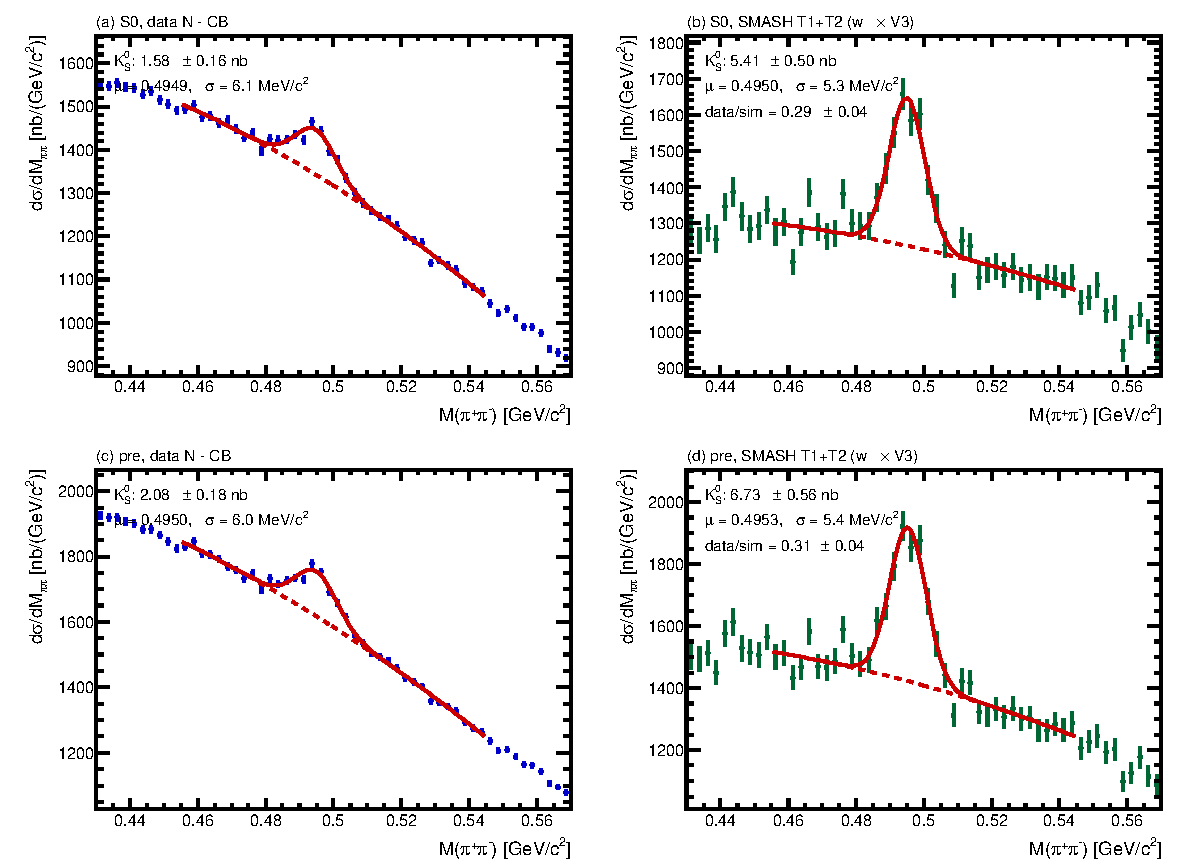
\includegraphics[width=0.72\textwidth]{figs_all/wp1_K0S.pdf}
\caption{K$^0_S\to\pipi$ peak in \Mpipi, summed over \Mfour$<1.10$\,\GeVcc.
Selection: top row (a, b) S0 (PT3 trigger, event vertex at $\vz>-160$\,mm, \betanew identification (pions $3\sigma$, leptons $5\sigma$ with a RICH ring), corrected momenta, all stored combinations (isBest $\ge0$), both pions in the event-vertex fit); bottom row (c, d) ``pre'' (the same without the pion-vertex condition); all \Mee, \Mfour below 1.10\,\GeVcc; SMASH $T_1+T_2$ with the same cuts.
(a, c) data $N-\mathrm{CB}$; (b, d) SMASH $T_1+T_2$; top row S0,
bottom row ``pre''. Red: Gaussian + pol2 $\chi^2$ fit in 0.455--0.545\,\GeVcc; dashed: the pol2 part. Normalisation as in
Fig.~\ref{fig:B1}. No fall-back involved.}
\label{fig:K0S}
\end{figure}

\subsection{Acceptance test of WP1 and the effect of the mass transfer}
\label{sec:wp1acc}
The specification asked that ``pre'' reproduces the first-study table \code{rw_compare_enriched.txt} $\times1.0161$ within 0.5\,\%
(bump 0.958, peak 1.233) with $J=1.44$--1.47. This report's chain, run at the settings of that table (simulated \Mfour not scaled,
$s=1$), gives B $0.9583\pm0.0133$ ($+0.01$\,\%), P $1.2332\pm0.0222$ ($-0.03$\,\%) and $J=1.4678\pm0.033$; every ratio of the old
table agrees to $4.8\times10^{-4}$ (the rounding of the table): \textbf{PASS}. With the nominal mass transfer of D8 ($s=0.99615$)
the same numbers are 0.9490 ($-0.96$\,\%), 1.2121 ($-1.73$\,\%) and $J=1.431\pm0.032$ ($-2.5$\,\%), because simulated entries move
across the window edges (``pre'': B 24.008 $\to$ 24.244\,nb, P 9.426 $\to$ 9.590\,nb). The shifts are 0.7, 1.0 and 1.2 statistical
errors. \flag{The specification's reference values hold for $s=1$; with D8 the references are 0.949 / 1.212 / 1.431 (``pre'') and
0.861 / 1.101 / 1.467 (S0).}

%======================================================================
\section{Data and SMASH after the typical \texorpdfstring{$\eta$}{eta} and X17 selection cuts}
\label{sec:e1}
%======================================================================
\inshort{at the analyst's request, the data are compared with SMASH after the cuts of earlier analyses (\cs{E1}--\cs{E4}: the angle between
the \pipi and \ee systems below $50^\circ$ in the laboratory and above $140^\circ$ in the $\eta$ rest frame, \Mpipi$<0.46$ or $0.42$\,\GeVcc,
with or without OA$>2^\circ$) and after OA$<6^\circ$ (\cs{X1}--\cs{X4}), on top of ``pre'' and of S0. SMASH as it is still lies below the data
just above the peak (the data exceed it by 16--45\,\%). With the $\eta$ channels $\times0.40$ and the non-$\eta$ background $\times$1.25--1.52
it describes the S0-based selections about as well as S0 itself. The cuts do not enrich the $\eta$, and they act on a simulated X17 as on the direct
decays: in a simple count none of them makes an X17 at the present limit easier to see than S0 alone. Drawn as in the earlier analysis (SMASH
scaled to the data integral), SMASH is right only in total; the three-scale fit of that approach does not measure the $\eta$, and its side-band
view cannot test X17 (\S\ref{sec:e1prev}). No other result of Part~III uses these cuts (D3).}

\notebox{\textbf{Names in this section.} \cs{E1}--\cs{E4}, \cs{E3oa}, \cs{E4oa} (sans-serif) are the cut sets of the earlier analyses, named as in
the first-study table \code{rw_compare_enriched.txt}; they are \emph{not} the \Mee classes E1 ($<10$\,\MeVcc) and E2 ($\ge10$\,\MeVcc) of the
rest of this report. \cs{X1}, \cs{X2}, \cs{X2old}, \cs{X3}, \cs{X4} are the selections with OA$<6^\circ$ (Table~\ref{tab:e1sel}). (a), (b), (c)
are the three ways SMASH is shown (as it is, scaled, display fit), not the ghost variant (a) of D6; $\delta$ is the mismatch per bin defined
below, not a systematic shift of \S\ref{sec:syst}. The figures and the package tables print the cut names in roman.}

\subsection{Why these cuts are used, and why Part~III does not use them}
\label{sec:e1why}
Earlier analyses of this channel (the cuts shown on earlier slides, \cs{E1}, and those of the old analysis code, \cs{E3}) select the combinations with
three kinematic cuts:
\begin{itemize}\setlength{\itemsep}{0pt}
\item $\alpha_{\mathrm{lab}}<50^\circ$: the angle between the \pipi system and the \ee system in the laboratory;
\item $\alpha_\eta>140^\circ$ (the ``$\eta$-rest angle''): the same angle in the rest frame of an $\eta$, i.e.\ in the frame of the four tracks
      computed with their mass set to $m_\eta$; in an $\eta$ decay the two systems fly apart back to back ($180^\circ$);
\item \Mpipi$<0.46$\,\GeVcc (0.42\,\GeVcc in the old code), below the K$^0_S$ mass;
\end{itemize}
often together with OA$>2^\circ$ on the \ee opening angle, whose usual purpose is to remove photon conversions (pairs with an almost zero
opening angle). The aim of these cuts is not so much to enhance the $\eta$ as to enhance a possible X17 signal, $\eta\to\pipi X17$,
$X17\to\ee$. The analyst has in addition proposed OA$<6^\circ$, because the \ee pairs of a light X17 are expected to have very small opening
angles.

Part~III does not use any of these cuts for its results (D3: no upper cuts on \MMfour, \Mpipi, the $\eta$-rest angle or OA), because Part~II
measured that they sculpt the spectrum and that the $\eta$-rest angle acts as a band-pass in \Mfour. The reason for the band-pass is simple
kinematics. In the rest frame of the four tracks the \pipi and \ee systems are \emph{always} back to back. The $\eta$ rest frame is this frame
when \Mfour$=m_\eta$, so every combination with \Mfour near $m_\eta$, $\eta$ or background, has $\alpha_\eta$ near $180^\circ$; away from $m_\eta$ the
frame is wrong and the angle falls. The cut therefore selects combinations by their \Mfour and cannot tell an $\eta$ from a background combination of the same
\Mfour. Still, this is the standard comparison of the earlier analyses, and the analyst asked to see it; it is given here in the conventions of
Part~III. None of its numbers is used elsewhere in this report.

\subsection{Selections and procedure}
\label{sec:e1proc}
\begin{enumerate}\setlength{\itemsep}{1pt}
\item \textbf{Selections} (Table~\ref{tab:e1sel}). Each cut set is applied on top of ``pre'' and on top of S0, which gives 22 selections.
      A plain name (\cs{E1}) means ``pre'' + \cs{E1}; S0\,+\,\cs{E1} means S0 + \cs{E1}; \cs{X4} is ``pre'' + OA$<6^\circ$ and \cs{X3} is S0 +
      OA$<6^\circ$. The cut definitions are those of the first study (\code{sim_eta_enriched.C}, \code{rw_compare_enriched.txt}); \cs{X2old}
      is the old code with its own OA flags ($2^\circ<$OA$<6^\circ$). The simulated entries are cut on the data-scale $\Mpipi'=0.9952\,\Mpipi$ of
      D8 (the first study cut the raw value).
\item \textbf{Data} (one pass, \code{e1_fill.C}, with the rules of the histogram factory \code{wp0_fill.C}): $N$ with event-group errors;
      CB $=2\sqrt{N_{++}N_{--}}$ in 10\,\MeVcc cells of \Mfour, interpolated to 2.5\,\MeVcc bins, $k=1$, errors from 200 like-sign replicas;
      in the \Mee and OA cells of the peak band the CB is spread by the like-sign share (\S\ref{sec:cb}). Cross sections:
      $(N-\mathrm{CB})\times64/63/L$, $L=6079.2\,\nbinv$.
\item \textbf{SMASH} (one pass, as in \S\ref{sec:before}): std + lep + $\eta$ sets, owned entries (mode A), $w\times$V3, $M_4'=0.99615\,M_4$,
      $T_1+T_2$ in nb. The $\eta$ channels are C2 + C3 + C4 + C5 + \Geta; the non-$\eta$ background is $G_{\pi^0D}+G_{\mathrm{conv}}+G_{\mathrm{vec}}
      +G_{\mathrm{oth}}$ ($=G_D+G_C$). The X17 is C6 per unit BR (17.000\,\MeVcc).
\item \textbf{Three ways to show SMASH.}
      (a) \emph{As it is}: every channel at its SMASH cross section $\times$ PDG BR $\times$ V3, nothing adjusted.
      (b) \emph{Scaled components}: all $\eta$ channels $\times0.40$ (the $\eta$ scale of Part~III: $\aP=0.418$, $\aEta=0.382$) and the non-$\eta$
      background $\times c_b$, with $c_b=[\mathrm{data}-0.40\,\eta]/\mathrm{non}$-$\eta$ in 0.575--0.70\,\GeVcc (the control region of stage A),
      one factor per selection.
      (c) \emph{Display fit}: data $=a_\eta\,\eta+c\,$non-$\eta$ in 0.40--0.70\,\GeVcc (60 bins of 5\,\MeVcc; errors: data, CB replicas and
      SMASH MC). It is not a yield: $c$ also absorbs the target-material counts (13--15\,\% of $N-\mathrm{CB}$, not simulated) and any CB deficit.
\item \textbf{How well SMASH describes the data} in 0.40--0.70\,\GeVcc (5\,\MeVcc bins): $\chi^2/\mathrm{ndf}$, and the mismatch $\delta$: the
      fraction of the model that must be added (in quadrature) to the error of every bin to bring $\chi^2/\mathrm{ndf}$ to 1. In plain words,
      $\delta=0.05$ means that the model misses a 5\,\MeVcc bin by about 5\,\% on average. Unlike $\chi^2/\mathrm{ndf}$, $\delta$ does not fall when
      a cut removes counts and the errors grow.
\item \textbf{X17 window} (\Mfour 0.5325--0.5575\,\GeVcc, \Mee 15.5--24.5\,\MeVcc). Per selection: the simulated X17 efficiency relative to S0,
      $\varepsilon_X/\varepsilon_X(\mathrm{S0})$; the data counts $N$ and the CB; the X17 counts at the present S0 limit,
      $N_X=392\times\mathrm{C6}(\mathrm{sel},\mathrm{window})/\mathrm{C6}(\mathrm{S0},\mathrm{X2D})$ (392 counts in the X2D range is the limit of
      \S\ref{sec:x17d}; $\mathrm{C6}(\mathrm{S0},\mathrm{X2D})=6257.53$\,nb per unit BR); the counting excess $Z=N_X/\sqrt{N+\mathrm{var\,CB}}$
      such an X17 would give; the counting proxy $\sqrt{N}/(\varepsilon_X/\varepsilon_X(\mathrm{S0}))/\sqrt{N_{\mathrm{S0}}}$, the relative size of
      the smallest X17 a simple count could see (smaller is better); and the S/B gain $(\varepsilon_X/\varepsilon_X(\mathrm{S0}))/(N/N_{\mathrm{S0}})$.
      These are counting estimates, not the frozen likelihood.
\item \textbf{Checks.} The chain reproduces the first study in its own convention (6080.5\,\nbinv, no 64/63, SMASH \Mfour not scaled): all 56
      rows of its section~1 (``pre'', \cs{E1}, \cs{E2}, \cs{E3}, \cs{E3oa}, \cs{E4}, \cs{E4oa} $\times$ 8 regions; each with data, SMASH and ratio) agree to the
      last printed digit (\code{tables_all/e1_repro.txt}). It also reproduces Part~III: S0 window P $N=55\,947$, CB $=3279.0\pm56.6$, 8.8012\,nb, $T_1+T_2=7.9961$\,nb; ``pre''
      $T_1+T_2$ in P 9.5901\,nb; C6(S0, X2D) $=6257.53$\,nb (x17d: 6257.5); the one-scale test of S0 $a=1.1905$, $\chi^2=724.4/59$ (WP1: 1.1911,
      723.7/59). An independent verification with its own code (e1v) recomputed eight of the selections and agrees to the printed digit;
      it corrected two statements of the package text, which are used corrected here (App.~\ref{app:recon}).
\end{enumerate}

\textbf{Old and new numbers.} The values quoted earlier for \cs{E1} (bump 0.98, peak 1.18, 0.56--0.70 1.35, 0.70--1.00 1.19) are in the
first-study convention. In the convention of Part~III they are 0.977 / 1.183 / 1.354 / 1.242. Three things change them: the factor 64/63 and
$L=6079.2$ ($+1.6$\,\%); the mass transfer of D8, which moves simulated entries across the steep edges ($-10$\,\% below the bump, $+4$\,\% at
0.70--1.00); and the \Mpipi scale of SMASH in the cut. The peak and 0.56--0.70 ratios hardly move (1.184 $\to$ 1.183, 1.347 $\to$ 1.354).

\begin{table}[tbp]
\centering
\caption{\textbf{What it shows: the cuts keep 32--81\,\% of the peak-window counts; every cut with OA$<6^\circ$ removes over 90\,\% of the CB.}
The 22 selections of this section: the cuts added to the base (``pre'' or S0) and the data counts (raw counts, isBest $\ge0$) in the peak window P
(0.53364--0.55416\,\GeVcc) with the CB $=2\sqrt{N_{++}N_{--}}$ ($k=1$), and in the X17 window (\Mfour 0.5325--0.5575\,\GeVcc, \Mee 15.5--24.5\,\MeVcc).
Names: on the ``pre'' base the plain name (\cs{E1}); on the S0 base S0\,+\,\cs{E1} etc.; the last row is \cs{X4} (``pre'' + OA$<6^\circ$) and
\cs{X3} (S0 + OA$<6^\circ$). $\alpha_{\mathrm{lab}}$, $\alpha_\eta$: angle between the \pipi and \ee systems in the laboratory and in the $\eta$
rest frame; \Mpipi in \GeVcc. With OA$<6^\circ$ the like-sign counts fall much more than the unlike-sign counts (``pre'': $N_{++}\times0.060$,
$N_{--}\times0.120$, $N\times0.75$), so the CB of these selections is only a lower limit (D5; \S\ref{sec:e1cav}). Source:
\code{tables_all/e1_table.txt}, section~1.}
\label{tab:e1sel}
\footnotesize
\setlength{\tabcolsep}{3.5pt}
\begin{tabularx}{\textwidth}{@{}l L r r r r r r@{}}
\toprule
 & & \multicolumn{3}{c}{base ``pre''} & \multicolumn{3}{c}{base S0} \\
\cmidrule(lr){3-5}\cmidrule(lr){6-8}
name & cuts added to the base & $N$ in P & CB in P & $N$ X17 win. & $N$ in P & CB in P & $N$ X17 win. \\
\midrule
(base) & none & 77\,513 & 7948.8 & 9167 & 55\,947 & 3279.0 & 6350 \\
\cs{E1} & $\alpha_{\mathrm{lab}}<50^\circ$, $\alpha_\eta>140^\circ$, \Mpipi$<0.46$, OA$>2^\circ$ (slides) & 46\,001 & 5627.5 & 7295 & 33\,317 & 2386.4 & 5221 \\
\cs{E2} & \cs{E1} without OA$>2^\circ$ & 59\,946 & 5743.4 & 7318 & 44\,333 & 2445.2 & 5237 \\
\cs{E3} & $\alpha_{\mathrm{lab}}<50^\circ$, $\alpha_\eta>140^\circ$, \Mpipi$<0.42$ (old code) & 51\,605 & 4984.3 & 6375 & 37\,976 & 2136.1 & 4546 \\
\cs{E3oa} & \cs{E3} + OA$>2^\circ$ & 39\,227 & 4887.0 & 6352 & 28\,239 & 2088.6 & 4530 \\
\cs{E4} & $\alpha_{\mathrm{lab}}<50^\circ$, $\alpha_\eta>140^\circ$ ($\eta$ band) & 61\,066 & 5911.0 & 7468 & 45\,209 & 2506.6 & 5341 \\
\cs{E4oa} & \cs{E4} + OA$>2^\circ$ & 46\,897 & 5790.6 & 7445 & 33\,997 & 2444.7 & 5325 \\
\cs{X1} & \cs{E2} + OA$<6^\circ$ & 42\,958 & 393.1 & 4137 & 32\,918 & 178.9 & 3027 \\
\cs{X2} & \cs{E2} + $2^\circ<$OA$<6^\circ$ & 29\,013 & 283.9 & 4114 & 21\,902 & 118.2 & 3011 \\
\cs{X2old} & \cs{E3} + $2^\circ<$OA$<6^\circ$ (old code with its OA flags) & 24\,715 & 216.5 & 3833 & 18\,541 & 75.7 & 2789 \\
\cs{X4} / \cs{X3} & OA$<6^\circ$ only & 54\,240 & 614.4 & 4275 & 40\,689 & 257.0 & 3100 \\
\bottomrule
\end{tabularx}
\end{table}

\subsection{SMASH as it is after the cuts}
\label{sec:e1asis}
Figures~\ref{fig:e1-m4E1} and \ref{fig:e1-m4X2} show the spectrum after the cuts of the slides (\cs{E1}) and after the same kinematic cuts
with $2^\circ<$OA$<6^\circ$ (\cs{X2}); Table~\ref{tab:e1R} gives the ratios of all 22 selections, and Fig.~\ref{fig:e1-regions} (top) shows them.
\begin{itemize}\setlength{\itemsep}{1pt}
\item \textbf{The excess above the peak stays.} After every cut the data lie above SMASH as it is just above the peak: data/SMASH in
      0.56--0.70\,\GeVcc is 1.23--1.45 on the ``pre'' base (``pre'' 1.350, \cs{E1} 1.354, \cs{E2} 1.286, \cs{E3} 1.232, \cs{X2} 1.445) and
      1.16--1.34 on the S0 base (S0 1.266, S0\,+\,\cs{E1} 1.267, S0\,+\,\cs{E2} 1.212, S0\,+\,\cs{E3} 1.161, S0\,+\,\cs{X2} 1.337). The data exceed
      SMASH as it is by 16--45\,\%; the cuts do not remove the mismatch.
\item In the bump window the ratio is 0.85--1.03, in the peak window 1.02--1.34, at 0.70--1.00\,\GeVcc 1.00--1.30.
\item \textbf{$\chi^2$ falls, the mismatch does not.} $\chi^2/\mathrm{ndf}$ of SMASH as it is in 0.40--0.70 falls after the cuts (``pre'' 79.2
      $\to$ \cs{E1} 29.5; S0 39.9 $\to$ S0\,+\,\cs{E1} 14.2), but only because the cuts remove counts (the cut sets with the angle cuts remove 38--81\,\% of the counts
      in 0.40--0.70, \cs{E1} 63\,\%; OA$<6^\circ$ alone 26--28\,\%) and the errors grow. The mismatch per bin does not shrink: $\delta$ goes from
      0.286 (``pre'') to 0.386 (\cs{E1}) and from 0.229 (S0) to 0.248 (S0\,+\,\cs{E1}); it is largest with OA$<6^\circ$ combined with the kinematic
      cuts (\cs{X2} 0.503, \cs{X2old} 0.466).
\end{itemize}

\begin{figure}[tbp]
\centering
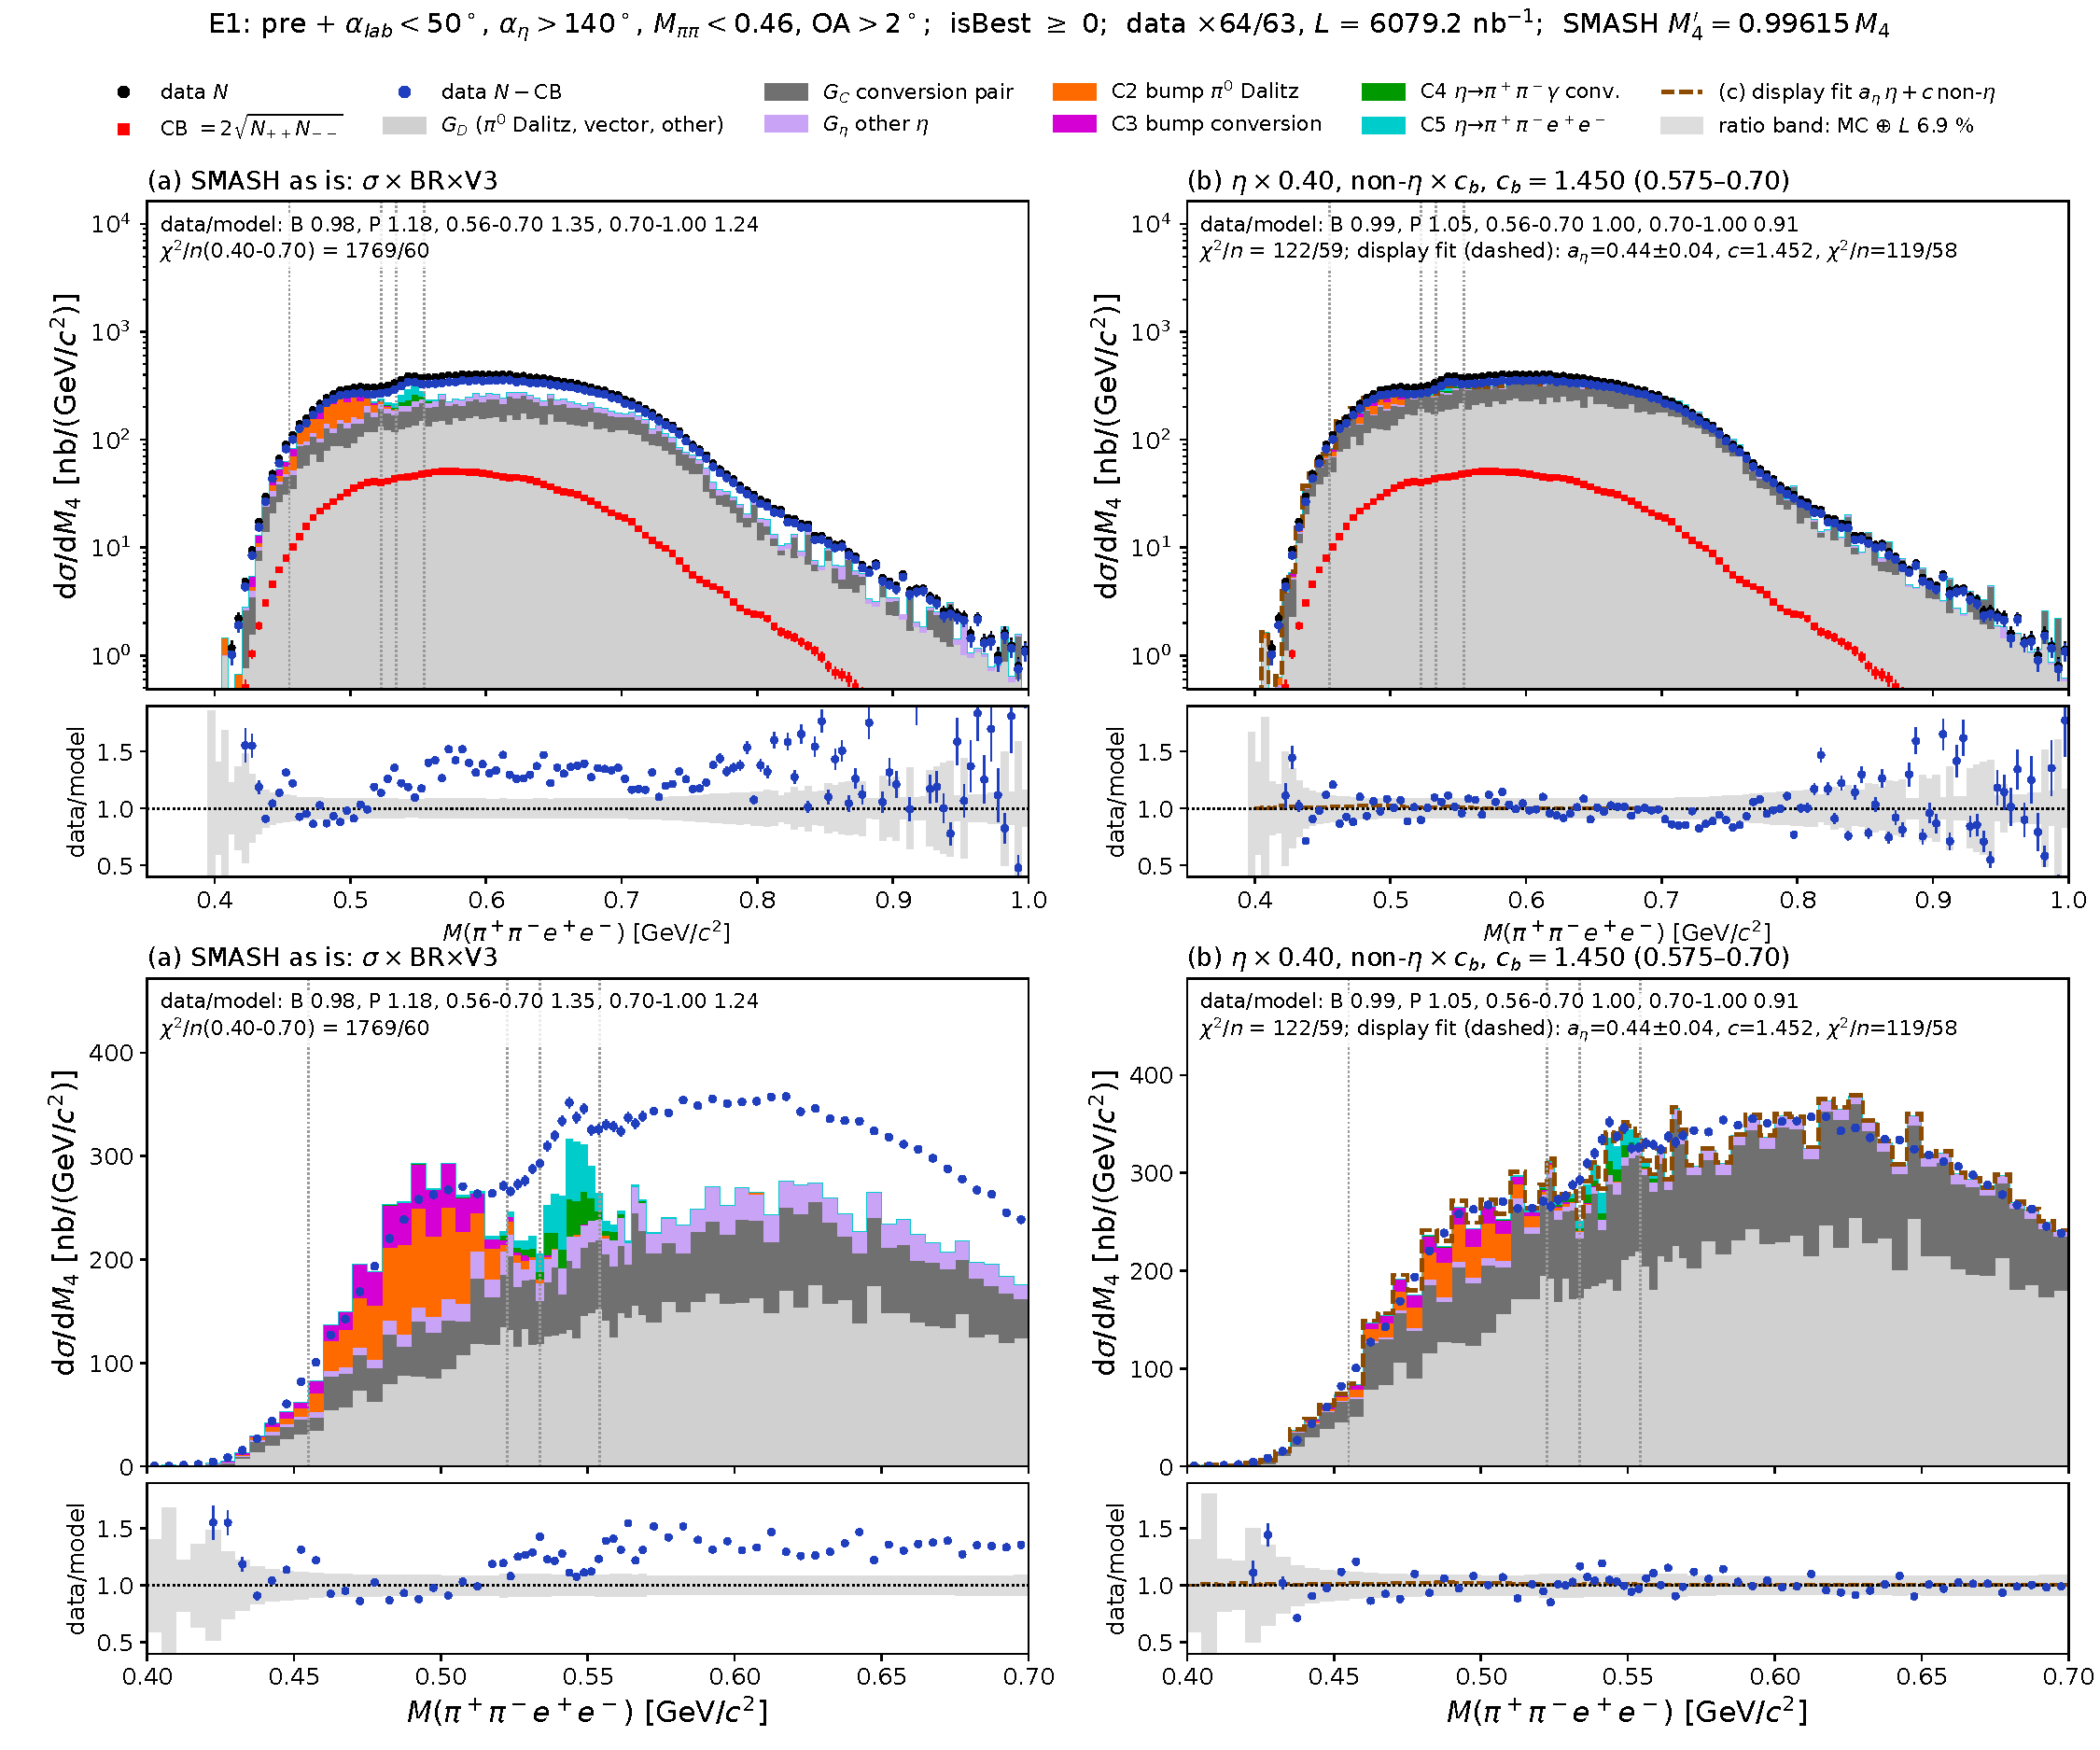
\includegraphics[width=0.97\textwidth]{figs_all/e1_m4_pre_E1_v2.pdf}
\caption{\textbf{What it shows: after the cuts of the slides (\cs{E1}) SMASH as it is still lies below the data above the peak; scaled, it follows them.}
Selection: data and SMASH with ``pre'' (PT3 trigger, event vertex in the target region ($\vz>-160$\,mm), \betanew particle identification (pions within $3\sigma$, leptons within $5\sigma$ and with a RICH ring), energy-loss-corrected momenta of all four tracks, all stored combinations of each event (isBest $\ge0$); no condition on the pions in the event-vertex fit), plus the cuts of the slides (\cs{E1}): $A$: $\alpha_{\mathrm{lab}}<50^\circ$ and $\alpha_\eta>140^\circ$ (angle between the \pipi and \ee systems in the laboratory, and in the $\eta$ rest frame), \Mpipi$<0.46$\,\GeVcc and the \ee opening angle OA$>2^\circ$; all \Mee; \Mfour 0.35--1.00\,\GeVcc (top, 5\,\MeVcc bins) and 0.40--0.70\,\GeVcc (bottom, 5\,\MeVcc bins, 2.5\,\MeVcc in 0.52--0.57); CB $=2\sqrt{N_{++}N_{--}}$ of the like-sign data with the same cuts (10\,\MeVcc cells of \Mfour, interpolated to 2.5\,\MeVcc bins, $k=1$); SMASH p+p at 4.5\,GeV (standard, lepton and $\eta$ sets, mode A) at its cross sections $\times$ PDG BR $\times$ the $\eta$-decay weights V3, masses moved to the data scale ($M_4'=0.99615\,M_4$, $\Mpipi'=0.9952\,\Mpipi$), same cuts (the \Mpipi cut on $\Mpipi'$); display (b): $\eta$ channels $\times0.40$, non-$\eta$ background $\times c_b$ fitted to the data in \Mfour 0.575--0.70\,\GeVcc (all \Mee and \Mpipi, one factor per selection); display fit (c) in \Mfour 0.40--0.70\,\GeVcc.
Data and SMASH after \cs{E1} $=$ ``pre'' + $\alpha_{\mathrm{lab}}<50^\circ$, $\alpha_\eta>140^\circ$, \Mpipi$<0.46$\,\GeVcc, OA$>2^\circ$ (isBest
$\ge0$). Top row: \Mfour 0.35--1.00\,\GeVcc, 5\,\MeVcc bins, log scale; bottom row: 0.40--0.70\,\GeVcc (5\,\MeVcc bins, 2.5\,\MeVcc in
0.52--0.57), linear. Data as $d\sigma/dM_4$ ($\times64/63$, $L=6079.2\,\nbinv$): $N$ black, CB $=2\sqrt{N_{++}N_{--}}$ from the like-sign data
red ($k=1$), $N-\mathrm{CB}$ blue. Stacked SMASH ($\sigma\times$PDG BR$\times$V3, mode A, $M_4'=0.99615\,M_4$): $G_D$ light grey, $G_C$ dark
grey, \Geta violet, C2 orange, C3 magenta, C4 green, C5 cyan. Left, (a): SMASH as it is. Right, (b): all $\eta$ channels $\times0.40$ and the
non-$\eta$ background $\times c_b$, $c_b=1.450$ fitted to the data in 0.575--0.70\,\GeVcc; dashed brown: the display fit (c),
$a_\eta\,\eta+c\,$non-$\eta$ in 0.40--0.70 (not a yield). Ratio pads: $(N-\mathrm{CB})$/model; grey band: SMASH MC $\oplus$ 6.9\,\% of $L$. The
panel text gives data/model in the windows B and P, in 0.56--0.70 and 0.70--1.00\,\GeVcc, and $\chi^2$ in 0.40--0.70. Dotted: windows B
and P. The package figure redrawn with the verifier's cosmetic corrections (\code{e1_m4_pre_E1_v2.pdf}; numbers unchanged).}
\label{fig:e1-m4E1}
\end{figure}

\begin{figure}[tbp]
\centering
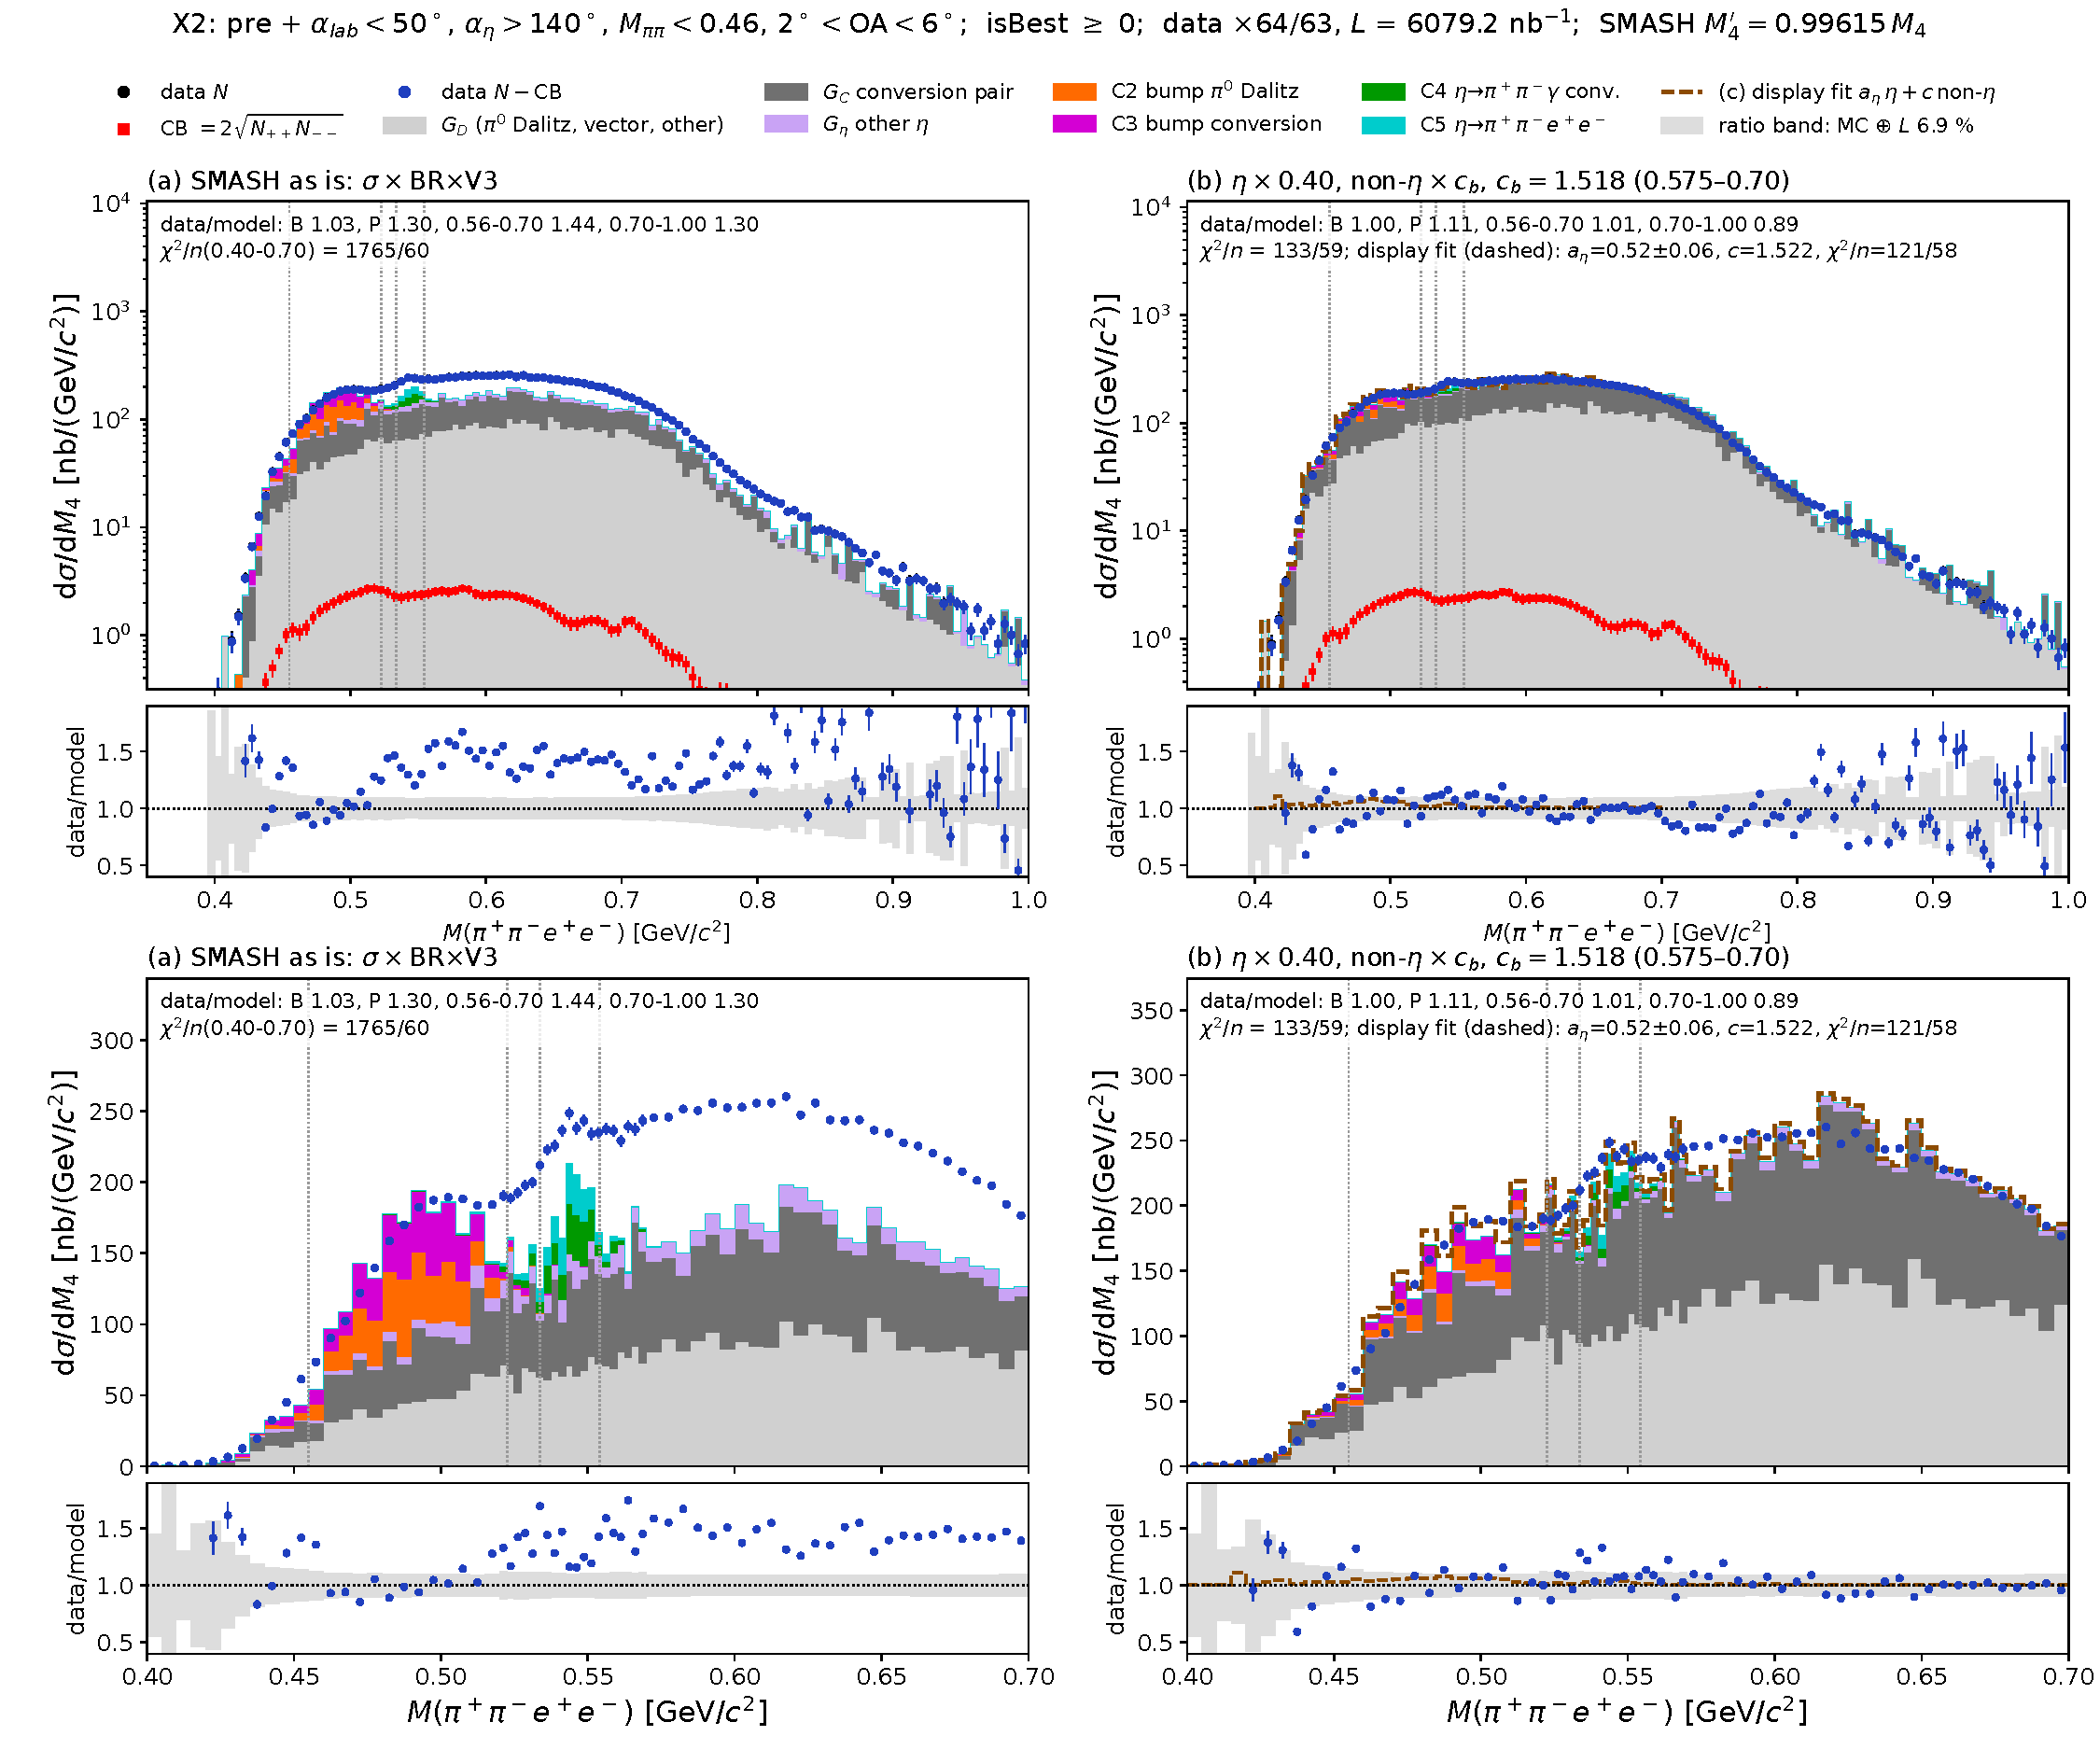
\includegraphics[width=0.97\textwidth]{figs_all/e1_m4_pre_X2_v2.pdf}
\caption{\textbf{What it shows: with the kinematic cuts and $2^\circ<$OA$<6^\circ$ (\cs{X2}) the data exceed SMASH as it is even more; scaled SMASH still follows them.}
Selection: data and SMASH with ``pre'' (PT3 trigger, event vertex in the target region ($\vz>-160$\,mm), \betanew particle identification (pions within $3\sigma$, leptons within $5\sigma$ and with a RICH ring), energy-loss-corrected momenta of all four tracks, all stored combinations of each event (isBest $\ge0$); no condition on the pions in the event-vertex fit), plus (\cs{X2}): $A$: $\alpha_{\mathrm{lab}}<50^\circ$ and $\alpha_\eta>140^\circ$ (angle between the \pipi and \ee systems in the laboratory, and in the $\eta$ rest frame), \Mpipi$<0.46$\,\GeVcc and the \ee opening angle $2^\circ<$OA$<6^\circ$; all \Mee; \Mfour 0.35--1.00\,\GeVcc (top, 5\,\MeVcc bins) and 0.40--0.70\,\GeVcc (bottom, 5\,\MeVcc bins, 2.5\,\MeVcc in 0.52--0.57); CB $=2\sqrt{N_{++}N_{--}}$ of the like-sign data with the same cuts (10\,\MeVcc cells of \Mfour, interpolated to 2.5\,\MeVcc bins, $k=1$); SMASH p+p at 4.5\,GeV (standard, lepton and $\eta$ sets, mode A) at its cross sections $\times$ PDG BR $\times$ the $\eta$-decay weights V3, masses moved to the data scale ($M_4'=0.99615\,M_4$, $\Mpipi'=0.9952\,\Mpipi$), same cuts (the \Mpipi cut on $\Mpipi'$); display (b): $\eta$ channels $\times0.40$, non-$\eta$ background $\times c_b$ fitted to the data in \Mfour 0.575--0.70\,\GeVcc (all \Mee and \Mpipi, one factor per selection); display fit (c) in \Mfour 0.40--0.70\,\GeVcc.
The same as Fig.~\ref{fig:e1-m4E1} for \cs{X2} $=$ ``pre'' + $\alpha_{\mathrm{lab}}<50^\circ$, $\alpha_\eta>140^\circ$, \Mpipi$<0.46$\,\GeVcc,
$2^\circ<$OA$<6^\circ$; $c_b=1.518$; data/SMASH as it is 1.445 in 0.56--0.70\,\GeVcc. With OA$<6^\circ$ the like-sign CB (red) is very small and
only a lower limit (D5), so the as-is ratios of this selection are upper values (\S\ref{sec:e1cav}).}
\label{fig:e1-m4X2}
\end{figure}

\begin{table}[p]
\centering
\caption{\textbf{What it shows: the data stay 16--45\,\% above SMASH as it is at 0.56--0.70\,\GeVcc after every cut; scaled, the bump window agrees.}
Data/SMASH per \Mfour region [\GeVcc]: (a) SMASH as it is; (b) $\eta\times0.40$, non-$\eta$ background $\times c_b$ (last column; fitted in
0.575--0.70, so (b) is close to 1 in 0.56--0.70). Errors (in \code{e1_table.txt}): B 0.013--0.024, P 0.021--0.044, 0.56--0.70 0.006--0.020, 0.70--1.00
0.002--0.032, without the common 6.9\,\% of $L$. Cut names in roman. Source: \code{tables_all/e1_tableR.tex}.}
\label{tab:e1R}
\footnotesize
\setlength{\tabcolsep}{4pt}\renewcommand{\arraystretch}{1.0}
\tabin{e1_tableR.tex}

\vspace{0.5em}
\caption{\textbf{What it shows: $\chi^2/\mathrm{ndf}$ falls after the cuts only because counts are removed; the mismatch $\delta$ and the scales stay.}
0.40--0.70\,\GeVcc, 5\,\MeVcc bins. $\chi^2/n$ of (a) SMASH as it is, (b) the scaled model, (c) the display fit; $\delta$: mismatch per bin;
$c_b$: non-$\eta$ factor of (b) (errors 0.008--0.024); $a_\eta$, $c$: the factors of the display fit (not yields); last column: data counts in
0.40--0.70. Source: \code{tables_all/e1_tableF.tex}.}
\label{tab:e1F}
\setlength{\tabcolsep}{3.5pt}
\tabin{e1_tableF_ra4.tex}
\end{table}

\subsection{SMASH with scaled components}
\label{sec:e1scaled}
In the spirit of the analyst's question (``the components can be scaled''), display (b) scales the two parts of SMASH: every $\eta$ channel by the
$\eta$ scale of Part~III, 0.40, and the non-$\eta$ background by one factor $c_b$ fitted above the peak. The display fit (c) lets both factors
float in 0.40--0.70\,\GeVcc. Figures~\ref{fig:e1-ovpre} and \ref{fig:e1-ovS0} show the result for nine selections of each base,
Fig.~\ref{fig:e1-regions} (middle, bottom) and Table~\ref{tab:e1F} all of them.
\begin{itemize}\setlength{\itemsep}{1pt}
\item \textbf{The background factor does not change.} $c_b$ is 1.25--1.52 in every selection (``pre'' 1.406, S0 1.321, \cs{E1} 1.450,
      S0\,+\,\cs{E1} 1.358): the non-$\eta$ background of SMASH must be raised by 25--52\,\% after every cut, as without the cuts.
\item \textbf{With the scaled components} the bump window agrees within 3\,\% (0.99--1.03) and 0.56--0.70 is close to 1 by construction (1.004--1.013; $c_b$ is set in
      0.575--0.70); the peak window
      keeps 4--16\,\% more data than the scaled model (1.04--1.16); at 0.70--1.00 the scaled model overshoots (0.76--0.92), because $c_b$, set at
      0.575--0.70, is too large for the higher masses.
\item \textbf{How well (b) describes the data} ($\delta$ in 0.40--0.70). On the S0 base the cut selections are described about as well as S0 itself:
      $\delta=0.050$ for S0 against 0.043--0.065 for S0\,+\,\cs{E1} \dots\ S0\,+\,\cs{E4oa}, and 0.054--0.077 with OA$<6^\circ$ (\cs{X3},
      S0\,+\,\cs{X1}, S0\,+\,\cs{X2}; S0\,+\,\cs{X2old} 0.109). On the ``pre'' base the description gets worse after the cuts: 0.058 for ``pre''
      against 0.071--0.117 for \cs{E1}--\cs{E4oa}, 0.093 for \cs{X1}, 0.163 for \cs{X2} and 0.202 for \cs{X2old} (\cs{X4} 0.065). So the typical
      cuts do not make SMASH describe the data better; with OA$<6^\circ$ added to the kinematic cuts it is worse.
\item \textbf{The $\eta$ scale does not change.} The display fit gives $a_\eta=0.418\pm0.028$ for ``pre'' and $0.399\pm0.025$ for S0, i.e.\ the
      $\eta$ scale 0.40 of Part~III. After the cuts it is 0.39--0.56, within 2.8$\sigma$ of 0.40 (\cs{E1} $0.443\pm0.043$, S0\,+\,\cs{E1}
      $0.442\pm0.038$, S0\,+\,\cs{E2} $0.410\pm0.030$, \cs{X3} $0.390\pm0.030$; the highest are \cs{X2old} $0.563\pm0.059$ and \cs{E4}, \cs{E4oa}
      0.489, 0.513, all at 2.8$\sigma$). A mild rise, not a different scale. $c$ of the fit follows $c_b$ (1.26--1.52; correlation with $a_\eta$
      $-0.50$ to $-0.73$).
\end{itemize}

\begin{figure}[tbp]
\centering
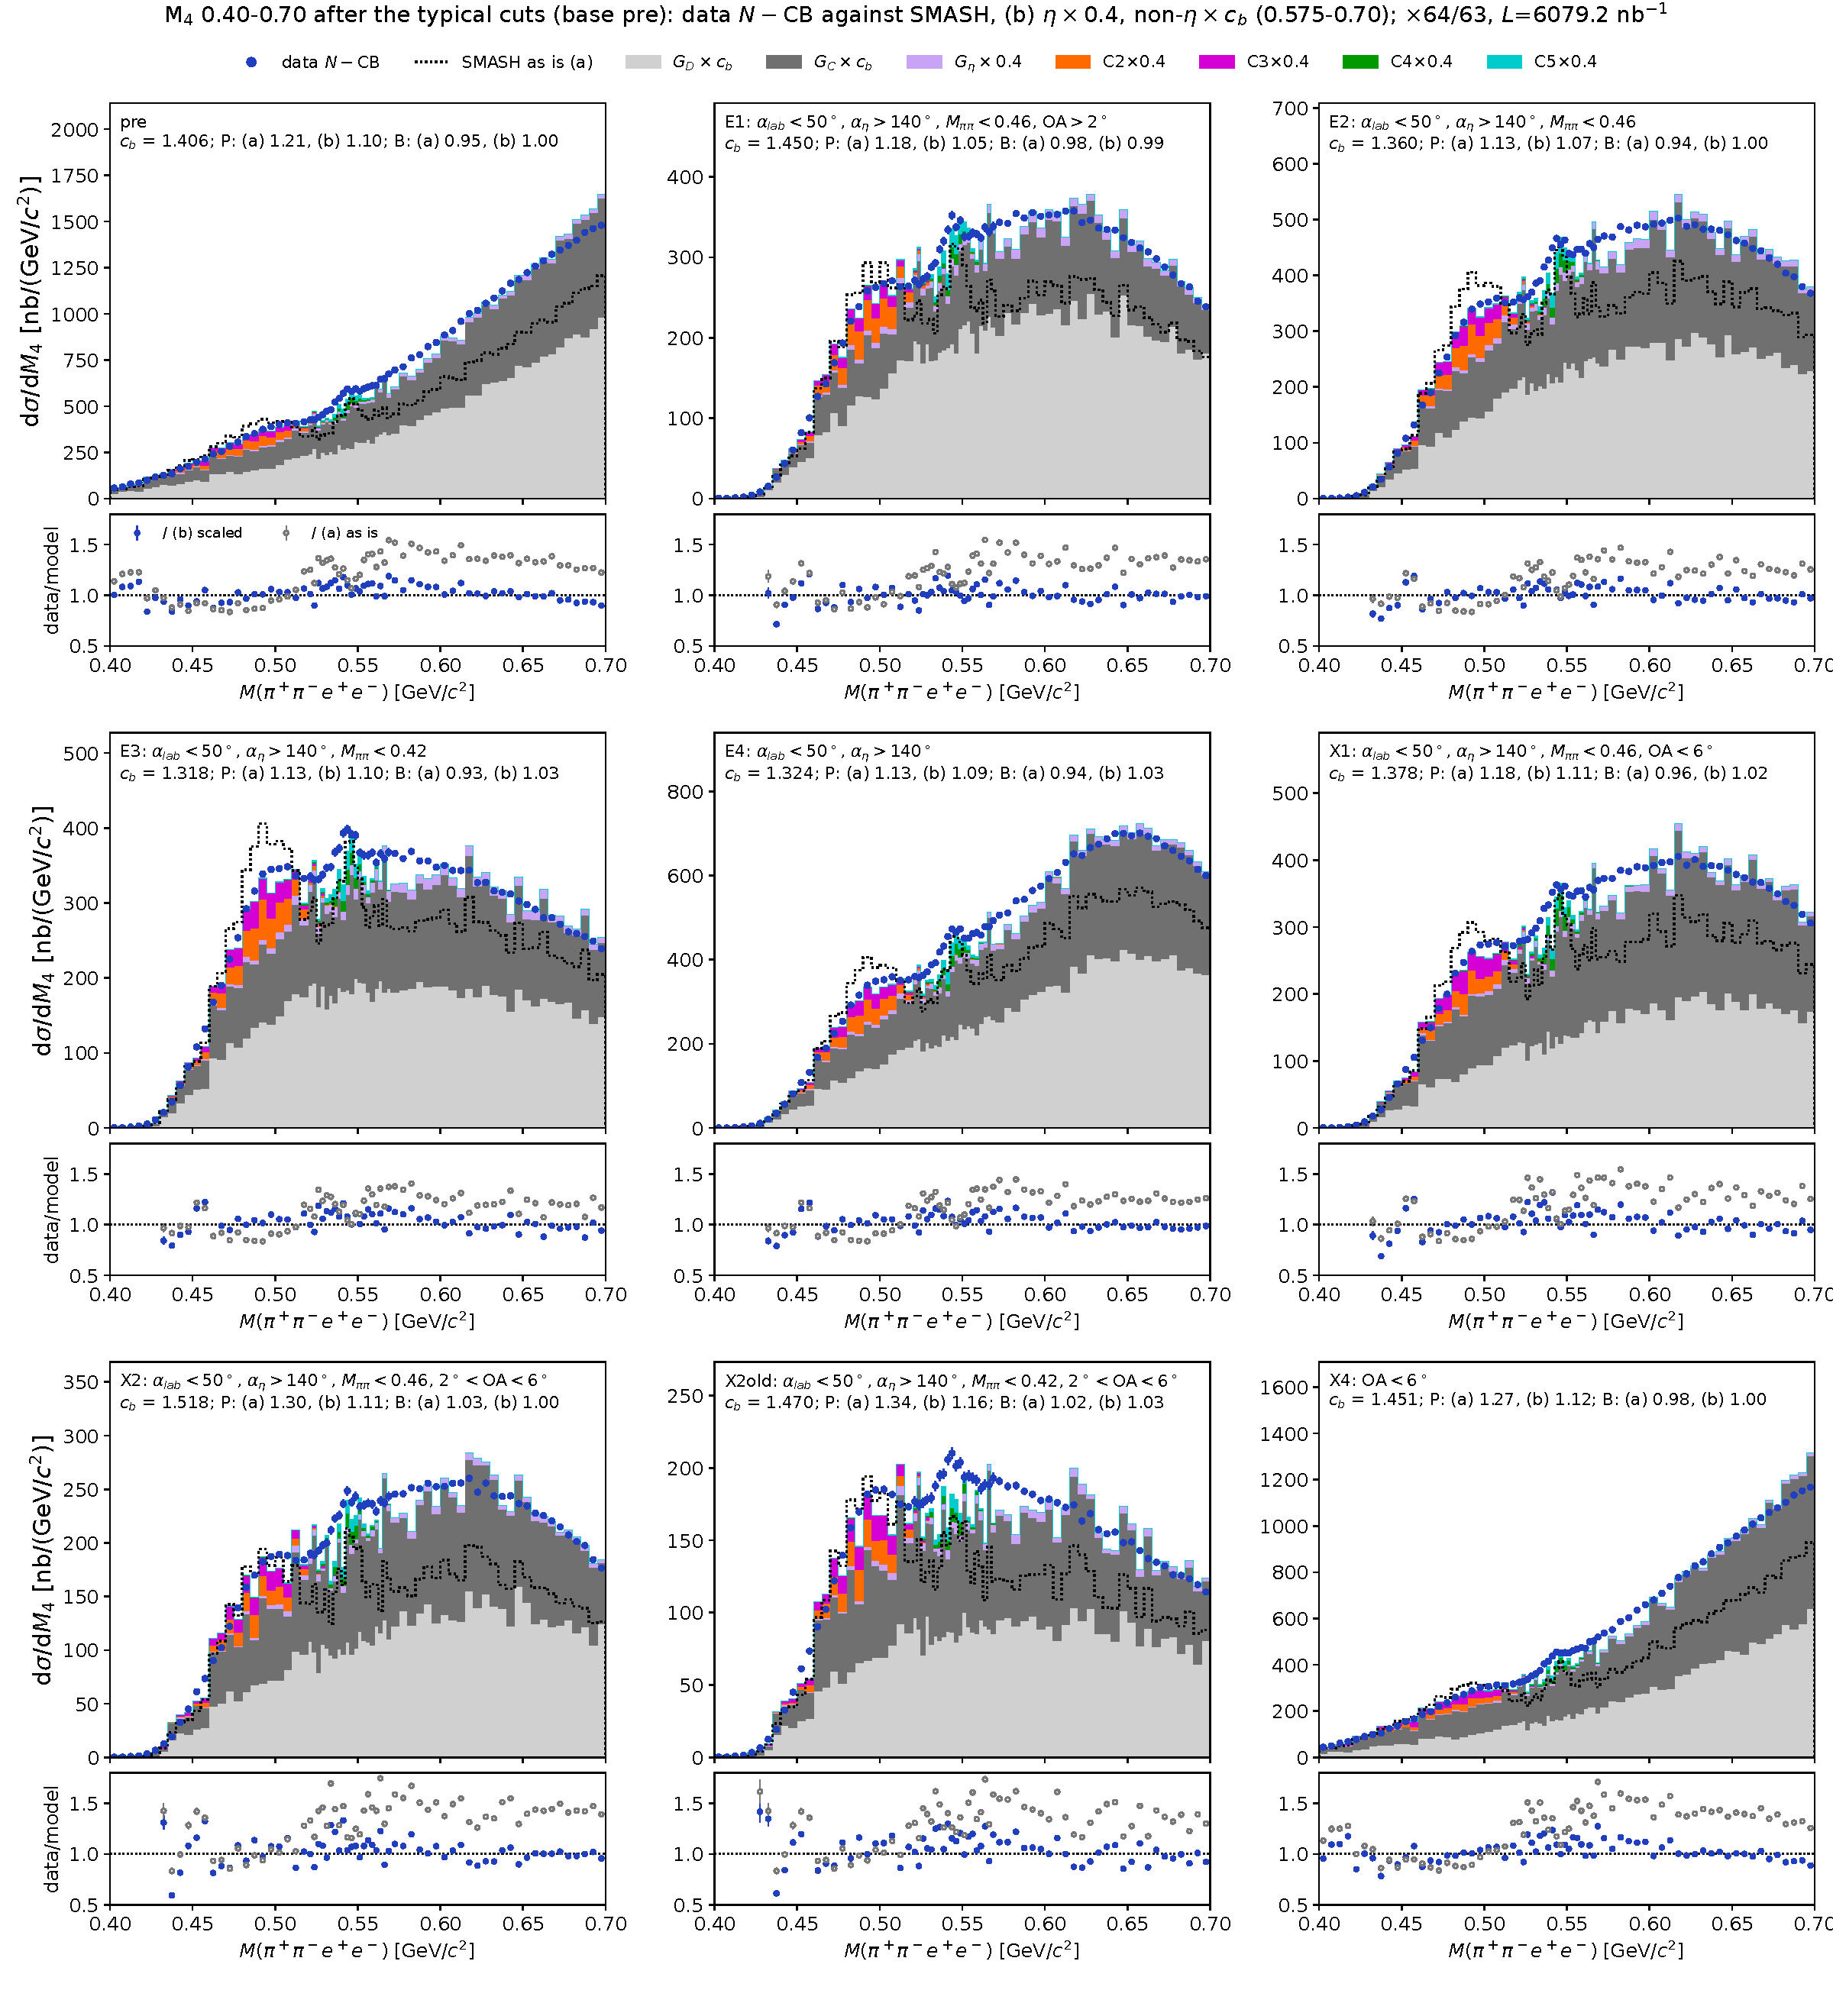
\includegraphics[width=\textwidth]{figs_all/e1_m4_overview_pre_v2.pdf}
\caption{\textbf{What it shows: on the ``pre'' base, after every cut, the data lie above SMASH as it is (dotted) above the peak; SMASH with scaled components follows them.}
Selection: data and SMASH (mode A, $w\times$V3, masses moved to the data scale), base ``pre'' (PT3 trigger, event vertex at $\vz>-160$\,mm, \betanew identification (pions $3\sigma$, leptons $5\sigma$ with a RICH ring), corrected momenta, all stored combinations (isBest $\ge0$), no pion-vertex condition), all \Mee, alone and with each cut set ($A$ = $\alpha_{\mathrm{lab}}<50^\circ$, $\alpha_\eta>140^\circ$; \Mpipi in \GeVcc: \cs{E1} $A$, \Mpipi$<0.46$, OA$>2^\circ$; \cs{E2} $A$, \Mpipi$<0.46$; \cs{E3} $A$, \Mpipi$<0.42$; \cs{E4} $A$; \cs{X1} \cs{E2} + OA$<6^\circ$; \cs{X2} \cs{E2} + $2^\circ<$OA$<6^\circ$; \cs{X2old} \cs{E3} + $2^\circ<$OA$<6^\circ$; \cs{X4} OA$<6^\circ$ alone); CB and (b) as in Fig.~\ref{fig:e1-m4E1}.
\Mfour 0.40--0.70\,\GeVcc (linear) for ``pre'' and eight cut selections (\cs{E1}, \cs{E2}, \cs{E3}, \cs{E4}, \cs{X1}, \cs{X2}, \cs{X2old},
\cs{X4} $=$ OA$<6^\circ$). Blue: data $N-\mathrm{CB}$; dotted black: SMASH as it is, (a); stack: (b), the non-$\eta$ background $G_D$, $G_C$
$\times c_b$ (greys) and the $\eta$ channels $\times0.4$ (\Geta violet, C2 orange, C3 magenta, C4 green, C5 cyan). The panel text gives $c_b$
and data/model in P and B for (a) and (b). Ratio pads: data/(b) (blue, full) and data/(a) (grey, open); bins where the model is below 2\,\% of
its maximum are not drawn. Normalisation as in Fig.~\ref{fig:e1-m4E1} (\code{e1_m4_overview_pre_v2.pdf}).}
\label{fig:e1-ovpre}
\end{figure}

\begin{figure}[tbp]
\centering
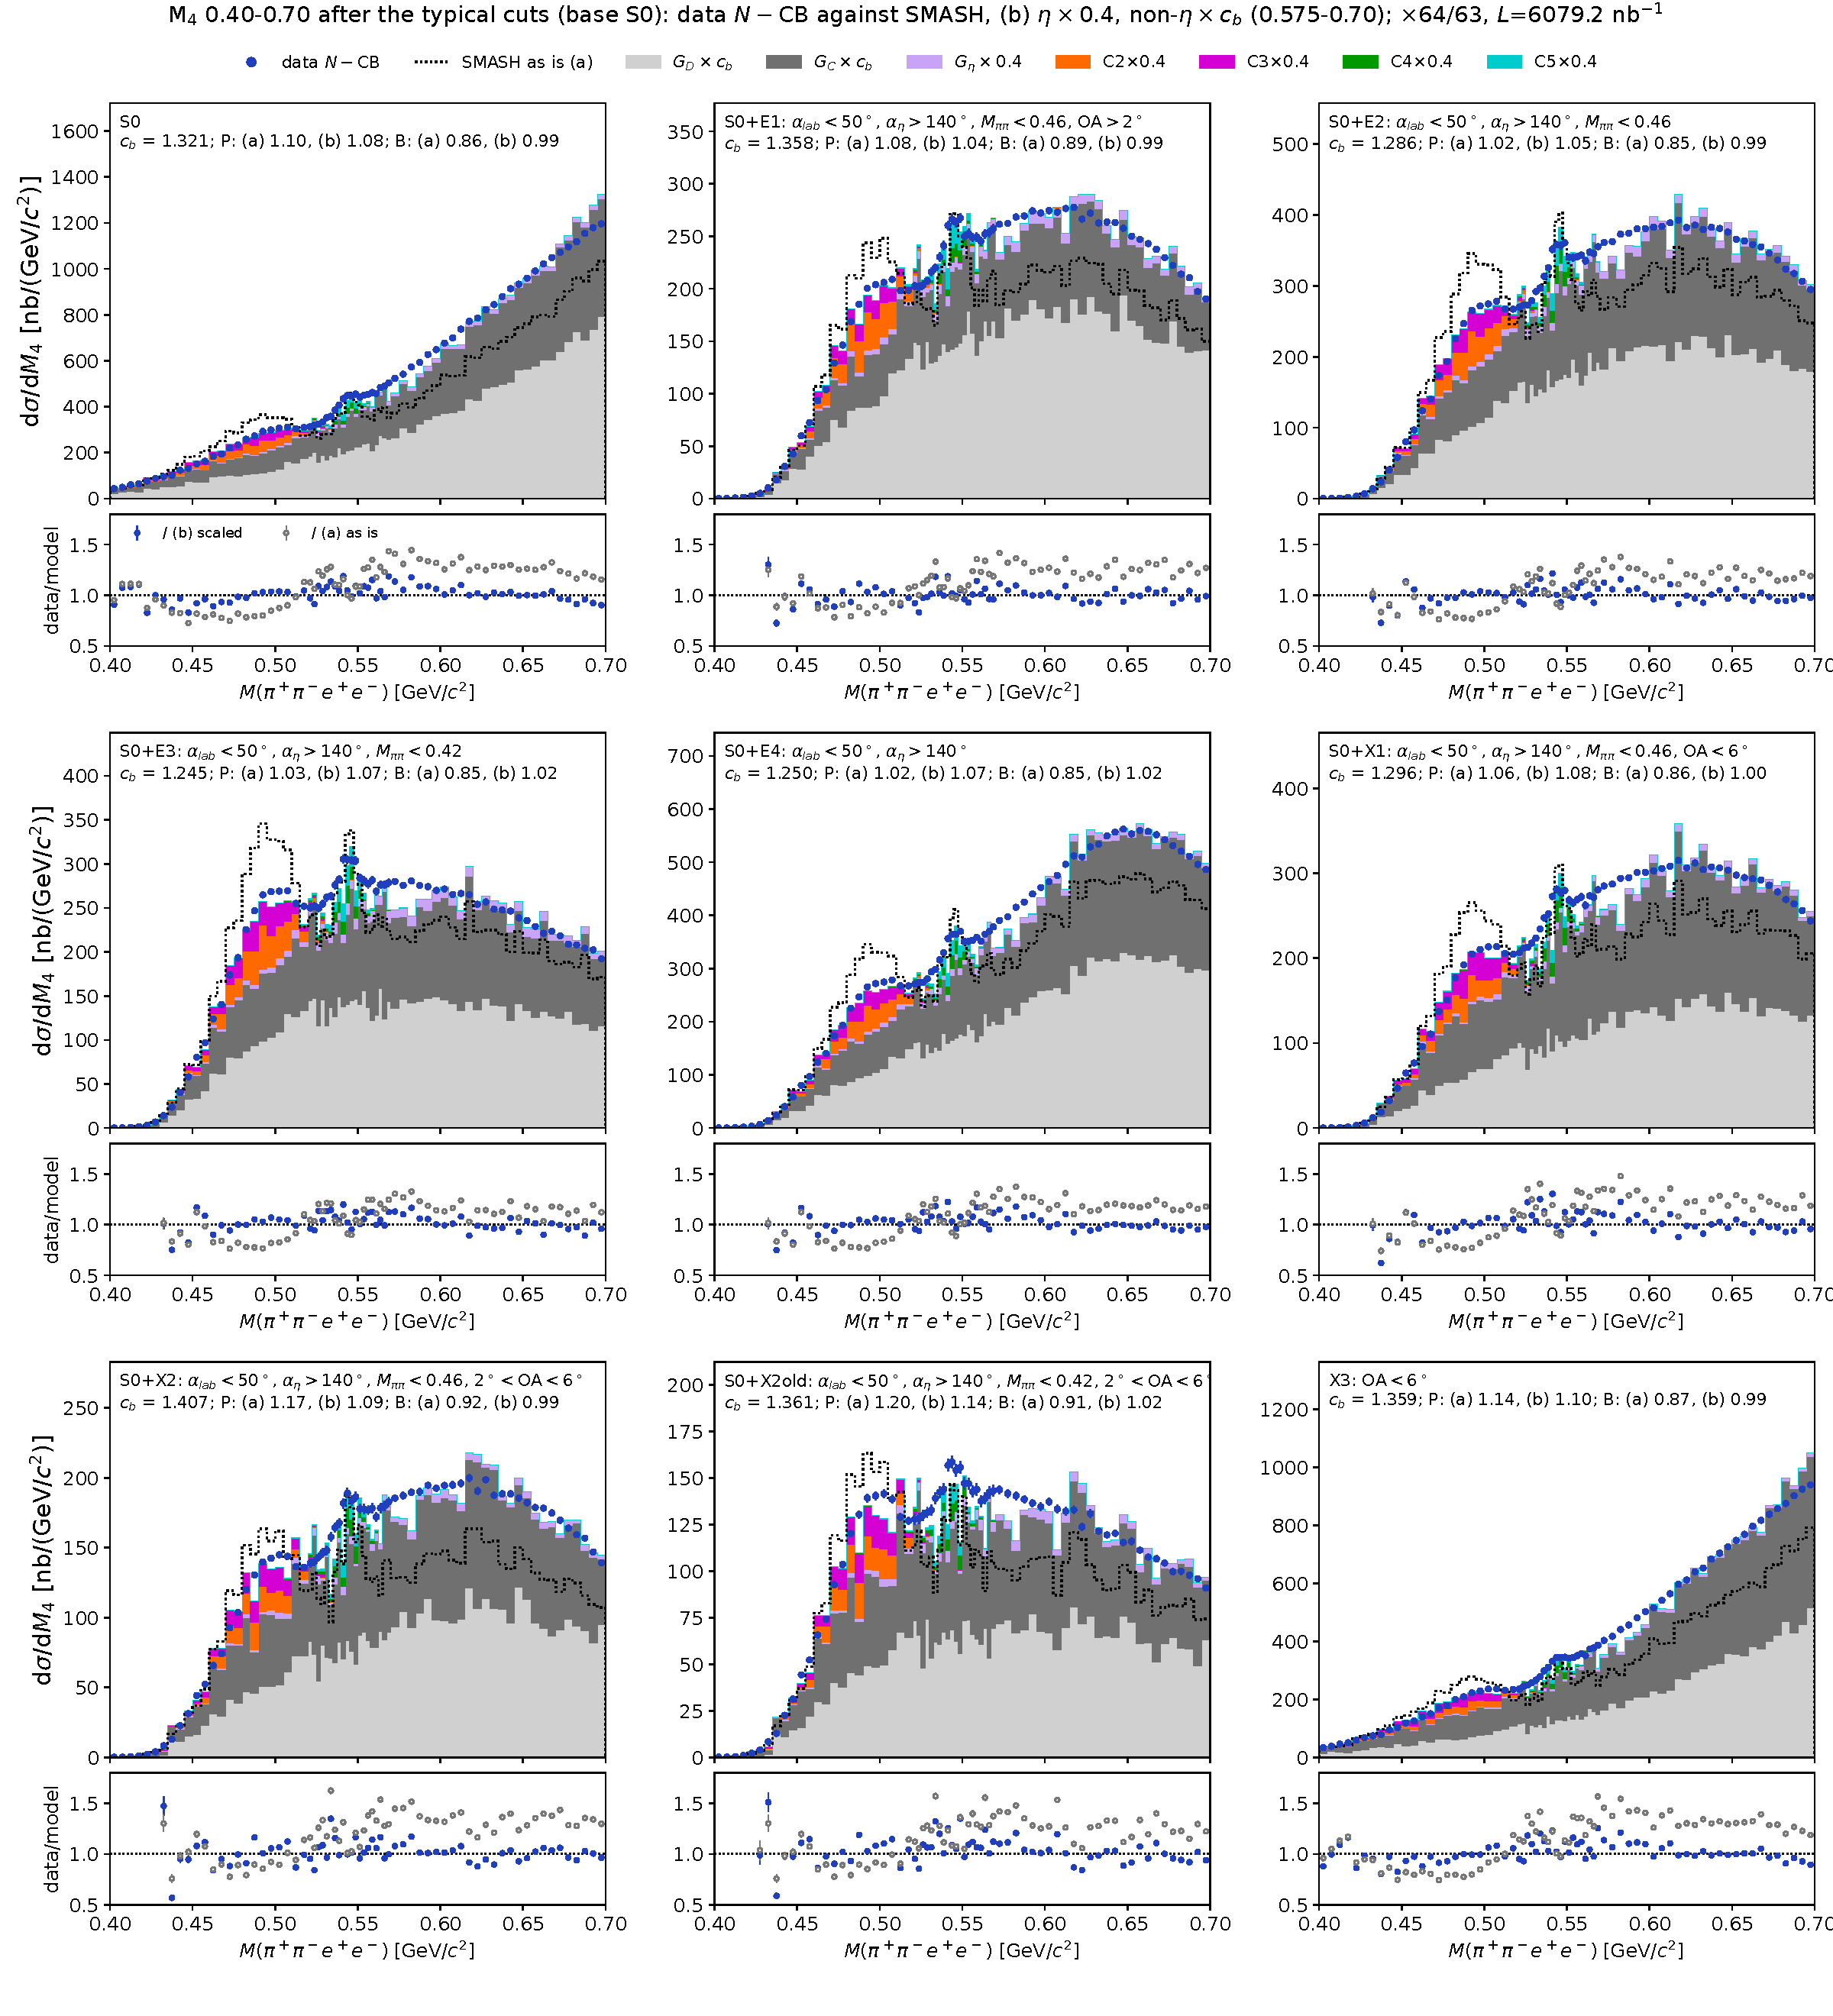
\includegraphics[width=\textwidth]{figs_all/e1_m4_overview_S0_v2.pdf}
\caption{\textbf{What it shows: on the S0 base the same: SMASH as it is stays below the data above the peak; scaled, it describes them as well as S0.}
Selection: data and SMASH (mode A, $w\times$V3, masses moved to the data scale), base S0 (PT3 trigger, event vertex at $\vz>-160$\,mm, \betanew identification (pions $3\sigma$, leptons $5\sigma$ with a RICH ring), corrected momenta, all stored combinations (isBest $\ge0$), both pions in the event-vertex fit), all \Mee, alone and with each cut set ($A$ = $\alpha_{\mathrm{lab}}<50^\circ$, $\alpha_\eta>140^\circ$; \Mpipi in \GeVcc: \cs{E1} $A$, \Mpipi$<0.46$, OA$>2^\circ$; \cs{E2} $A$, \Mpipi$<0.46$; \cs{E3} $A$, \Mpipi$<0.42$; \cs{E4} $A$; \cs{X1} \cs{E2} + OA$<6^\circ$; \cs{X2} \cs{E2} + $2^\circ<$OA$<6^\circ$; \cs{X2old} \cs{E3} + $2^\circ<$OA$<6^\circ$; \cs{X3} OA$<6^\circ$ alone); \Mfour 0.40--0.70\,\GeVcc (5\,\MeVcc bins, 2.5\,\MeVcc in 0.52--0.57); CB $=2\sqrt{N_{++}N_{--}}$ of the like-sign data with the same cuts (10\,\MeVcc cells of \Mfour, interpolated to 2.5\,\MeVcc bins, $k=1$); display (b): $\eta$ channels $\times0.40$, non-$\eta$ background $\times c_b$ fitted to the data in \Mfour 0.575--0.70\,\GeVcc (all \Mee and \Mpipi, one factor per selection).
As Fig.~\ref{fig:e1-ovpre} for S0 and the eight cut selections on S0 (S0\,+\,\cs{E1} \dots\ S0\,+\,\cs{X2old}, \cs{X3} $=$ S0 + OA$<6^\circ$)
(\code{e1_m4_overview_S0_v2.pdf}).}
\label{fig:e1-ovS0}
\end{figure}

\begin{figure}[tbp]
\centering
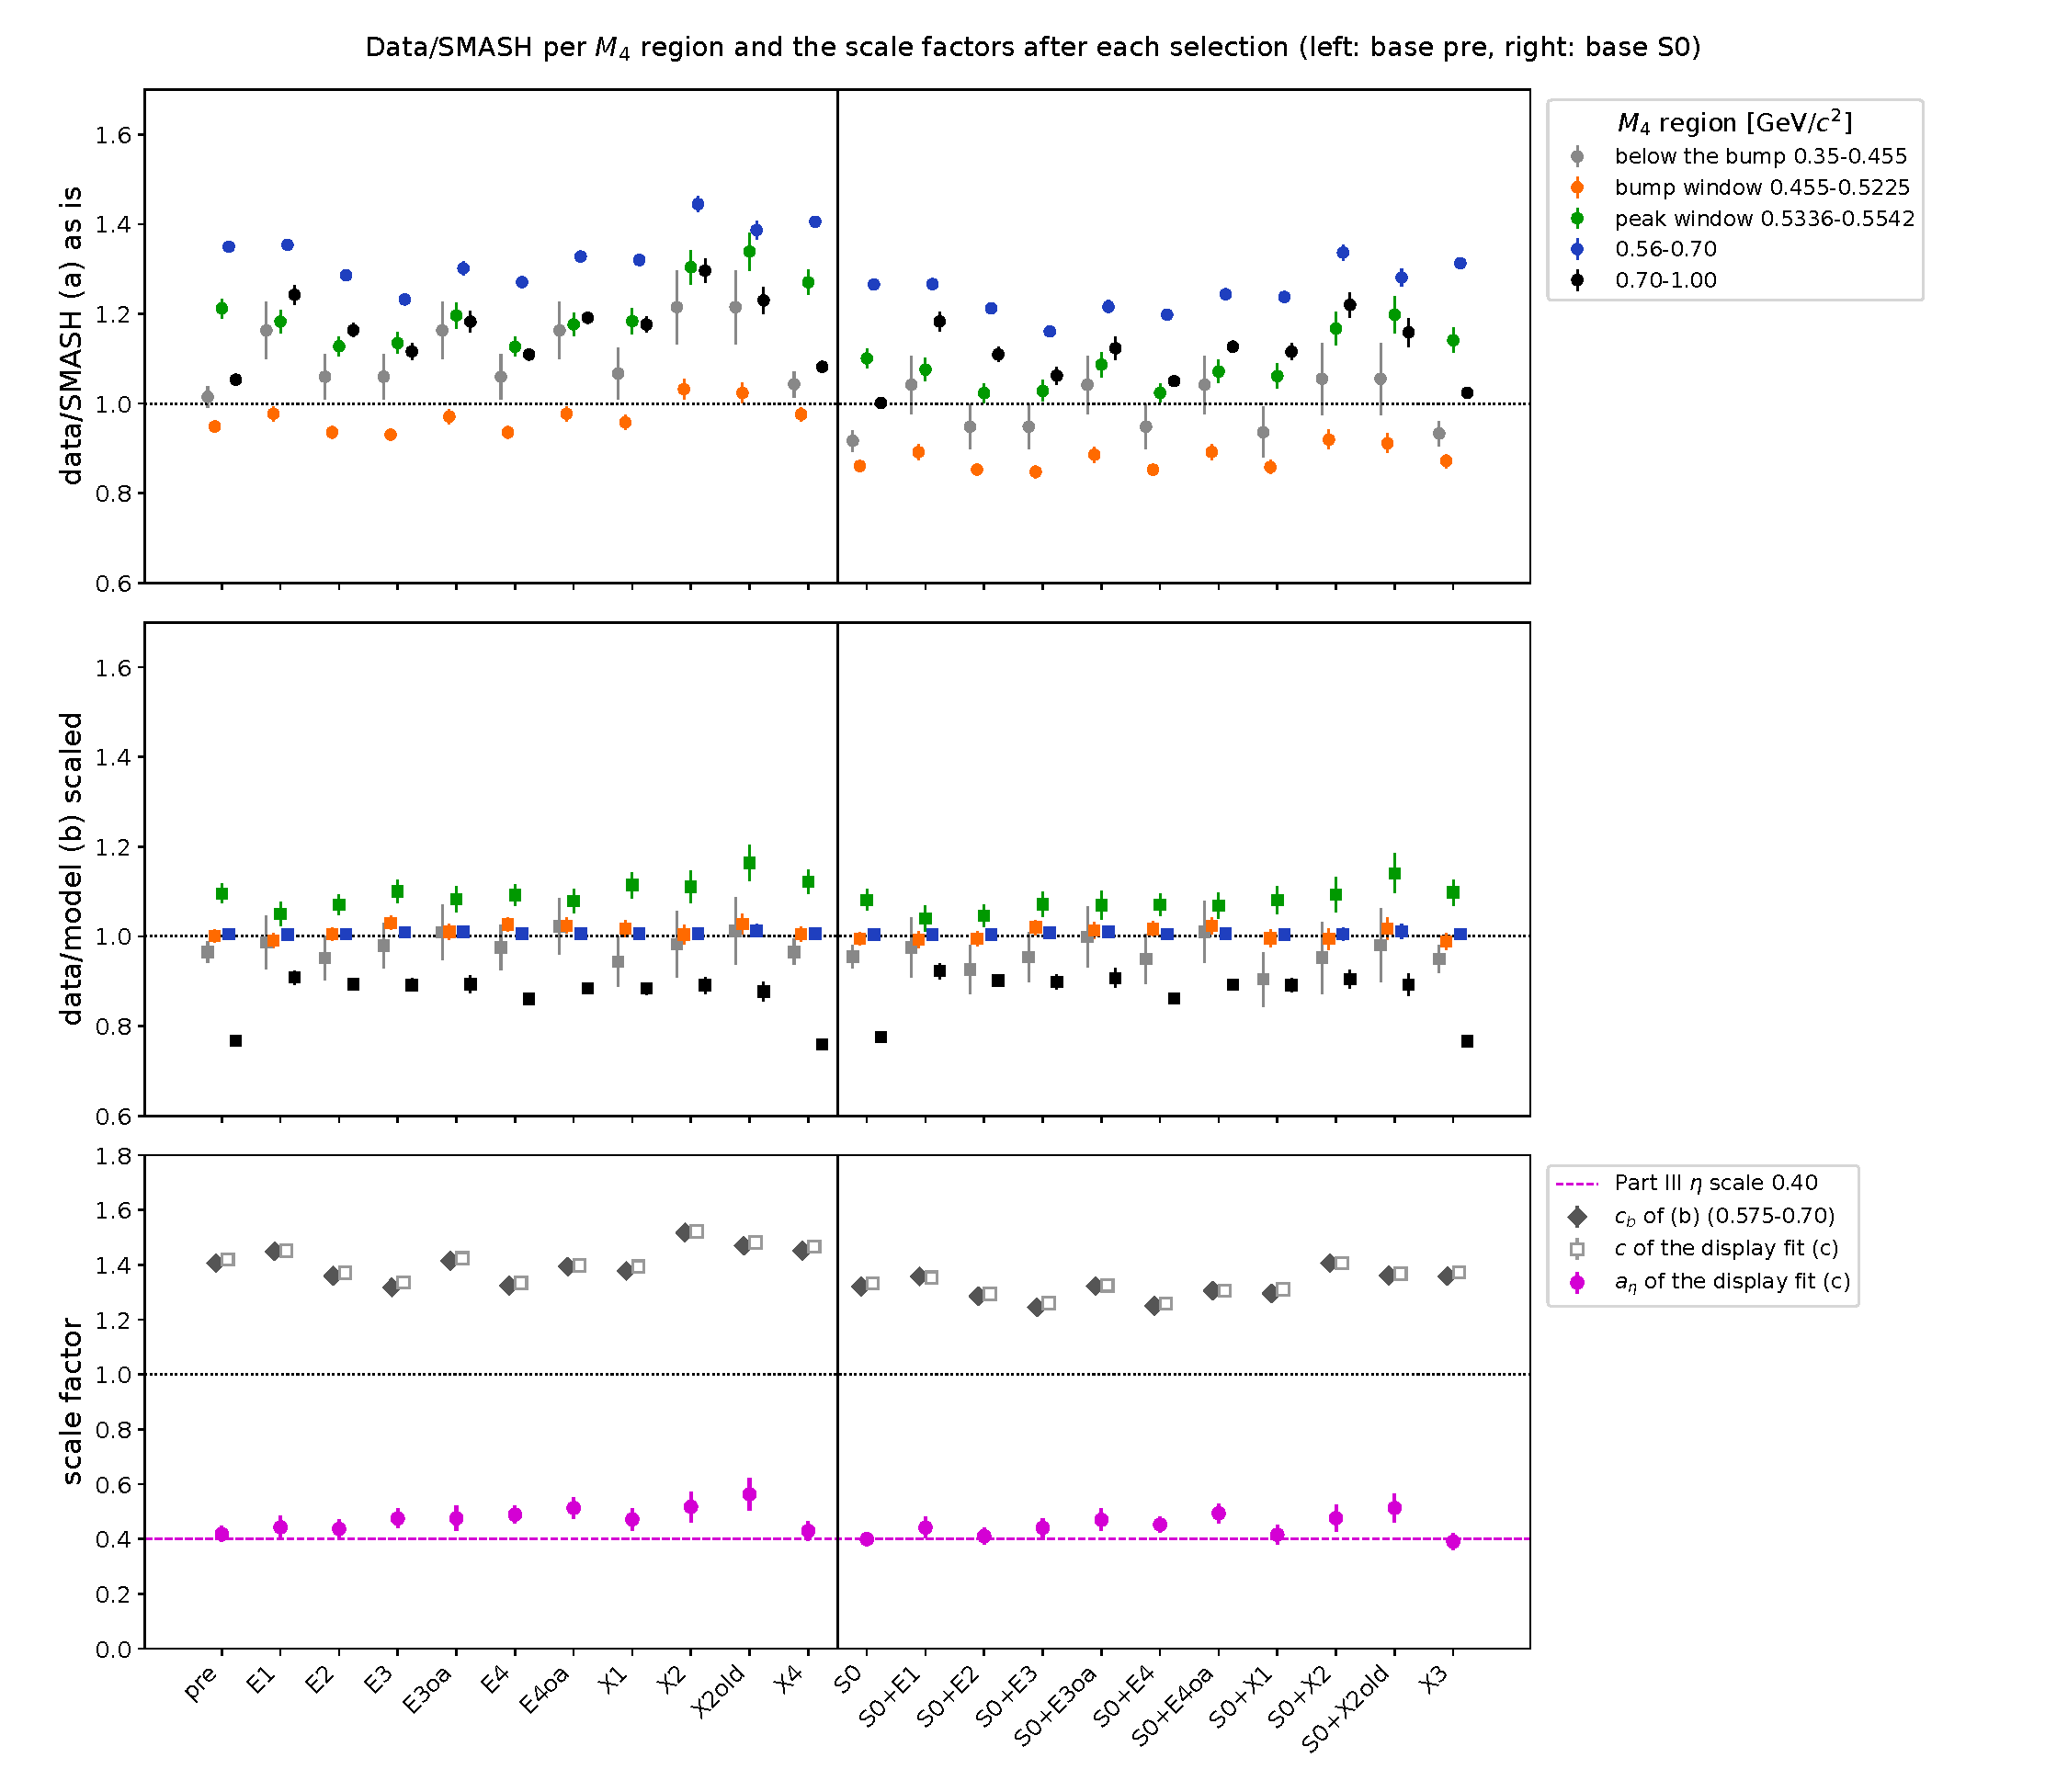
\includegraphics[width=0.92\textwidth]{figs_all/e1_regions.pdf}
\caption{\textbf{What it shows: no cut brings SMASH as it is to the data; scaled, the picture and the scale factors are the same with and without cuts.}
Selection: data and SMASH with ``pre'' (PT3 trigger, event vertex in the target region ($\vz>-160$\,mm), \betanew particle identification (pions within $3\sigma$, leptons within $5\sigma$ and with a RICH ring), energy-loss-corrected momenta of all four tracks, all stored combinations of each event (isBest $\ge0$); no condition on the pions in the event-vertex fit) (left) and S0 (PT3 trigger, event vertex in the target region ($\vz>-160$\,mm), \betanew particle identification (pions within $3\sigma$, leptons within $5\sigma$ and with a RICH ring), energy-loss-corrected momenta of all four tracks, all stored combinations of each event (isBest $\ge0$), both pions in the event-vertex fit) (right), each alone and with one cut set, with $A$: $\alpha_{\mathrm{lab}}<50^\circ$ and $\alpha_\eta>140^\circ$ (angle between the \pipi and \ee systems in the laboratory, and in the $\eta$ rest frame) and OA the \ee opening angle: \cs{E1}: $A$, \Mpipi$<0.46$\,\GeVcc, OA$>2^\circ$; \cs{E2}: $A$, \Mpipi$<0.46$\,\GeVcc; \cs{E3}: $A$, \Mpipi$<0.42$\,\GeVcc; \cs{E4}: $A$; \cs{X1}: \cs{E2}, OA$<6^\circ$; \cs{X2}: \cs{E2}, $2^\circ<$OA$<6^\circ$; \cs{X2old}: \cs{E3}, $2^\circ<$OA$<6^\circ$; \cs{E3oa}: \cs{E3}, OA$>2^\circ$; \cs{E4oa}: \cs{E4}, OA$>2^\circ$; OA$<6^\circ$ alone (\cs{X4} on ``pre'', \cs{X3} on S0); all \Mee; \Mfour regions 0.35--0.455, 0.4550--0.5225 (bump window), 0.53364--0.55416 (peak window), 0.56--0.70 and 0.70--1.00\,\GeVcc; CB $=2\sqrt{N_{++}N_{--}}$ of the like-sign data with the same cuts (10\,\MeVcc cells of \Mfour, interpolated to 2.5\,\MeVcc bins, $k=1$); SMASH p+p at 4.5\,GeV (standard, lepton and $\eta$ sets, mode A) at its cross sections $\times$ PDG BR $\times$ the $\eta$-decay weights V3, masses moved to the data scale ($M_4'=0.99615\,M_4$, $\Mpipi'=0.9952\,\Mpipi$), same cuts (the \Mpipi cut on $\Mpipi'$); display (b): $\eta$ channels $\times0.40$, non-$\eta$ background $\times c_b$ fitted to the data in \Mfour 0.575--0.70\,\GeVcc (all \Mee and \Mpipi, one factor per selection); display fit (c) in \Mfour 0.40--0.70\,\GeVcc (5\,\MeVcc bins).
Data/SMASH per \Mfour region for the 22 selections (left: ``pre'' base, right: S0 base). Top: (a), SMASH as it is. Middle: (b), $\eta\times0.40$
and non-$\eta\times c_b$ (0.56--0.70 close to 1 by construction). Bottom: $c_b$ (diamonds), $c$ of the display fit (open squares) and $a_\eta$ of the
display fit (magenta), with the Part~III $\eta$ scale 0.40 dashed. Regions: below the bump 0.35--0.455, B, P, 0.56--0.70, 0.70--1.00\,\GeVcc.
Errors: data statistics (event groups) $\oplus$ CB replicas $\oplus$ SMASH MC; the 6.9\,\% of $L$ is common and not included.}
\label{fig:e1-regions}
\end{figure}

\subsection{Do the cuts enrich the \texorpdfstring{$\eta$}{eta}?}
\label{sec:e1eta}
No. In SMASH the $\eta$ share of the bump window goes from 0.455 (``pre'') to 0.442 (\cs{E1}), and that of the peak window from 0.298 to 0.308
(S0: 0.329 $\to$ 0.338; Table~\ref{tab:e1sum}). Over all 22 selections the $\eta$ share of the peak window stays between 0.298 and 0.350. The cuts
remove $\eta$ and background combinations in about the same proportion. Only the direct decays gain a little in the peak window: from 4.2\,\% to 5.1\,\%
of the scaled model (S0: 5.1\,\% $\to$ 6.2\,\%). This is what the argument of \S\ref{sec:e1why} predicts: inside a narrow \Mfour window the
$\eta$-rest angle cannot tell an $\eta$ from a background combination.

\subsection{The opening angle of X17 pairs}
\label{sec:e1oa}
The idea behind OA$<6^\circ$ is that X17 pairs are close. Figure~\ref{fig:e1-x17oa} and Table~\ref{tab:e1oaf} test it with the simulated X17
(C6, 17.000\,\MeVcc, from $\eta\to\pipi X17$) in the HADES acceptance, selection S0, $\eta$ peak band.
\begin{itemize}\setlength{\itemsep}{1pt}
\item \textbf{Most X17 pairs are below $6^\circ$.} 67\,\% of the simulated X17 has OA$<6^\circ$ and 62\,\% has $2^\circ<$OA$<6^\circ$; in the X17
      window (\Mee 15.5--24.5\,\MeVcc, where the line lies after the resolution) the values are 58\,\% and 57\,\%. So the expectation is right,
      but a third of the X17 (42\,\% in the window) has OA$>6^\circ$ and would be lost by the cut.
\item \textbf{The reason is kinematics.} A pair of mass $m$ and momentum $p$ has its smallest opening angle when the two leptons share the energy
      equally, $\tan(\mathrm{OA}/2)=m/p$. A 17\,\MeVcc pair can therefore have OA$<6^\circ$ only if $p>17/\tan3^\circ=324$\,\MeVc. The
      simulated X17 pairs have a median momentum of 424\,\MeVc, and 73\,\% of them are above this momentum; unequal sharing makes the angle
      larger.
\item \textbf{The same holds for every pair of the same mass.} In the X17 window 57\,\% of the direct decays C5 and 50\,\% of the data
      $N-\mathrm{CB}$ have OA$<6^\circ$ (X17: 58\,\%). At a fixed \Mee the opening angle is set by the pair momentum and the energy sharing, not
      by the origin of the pair, so OA$<6^\circ$ acts mainly as a cut on the pair momentum. Over all \Mee the cut mostly removes pairs of larger
      mass, which the X17 fit separates anyway in its \Mee bins.
\item In the peak band the data follow the scaled SMASH in OA (in the X17 window up to about $12^\circ$; above it the few data counts lie
      higher), and an X17 at the present limit would be only a few per cent of the counts at almost every angle (Fig.~\ref{fig:e1-oa}).
\end{itemize}

\begin{figure}[tbp]
\centering
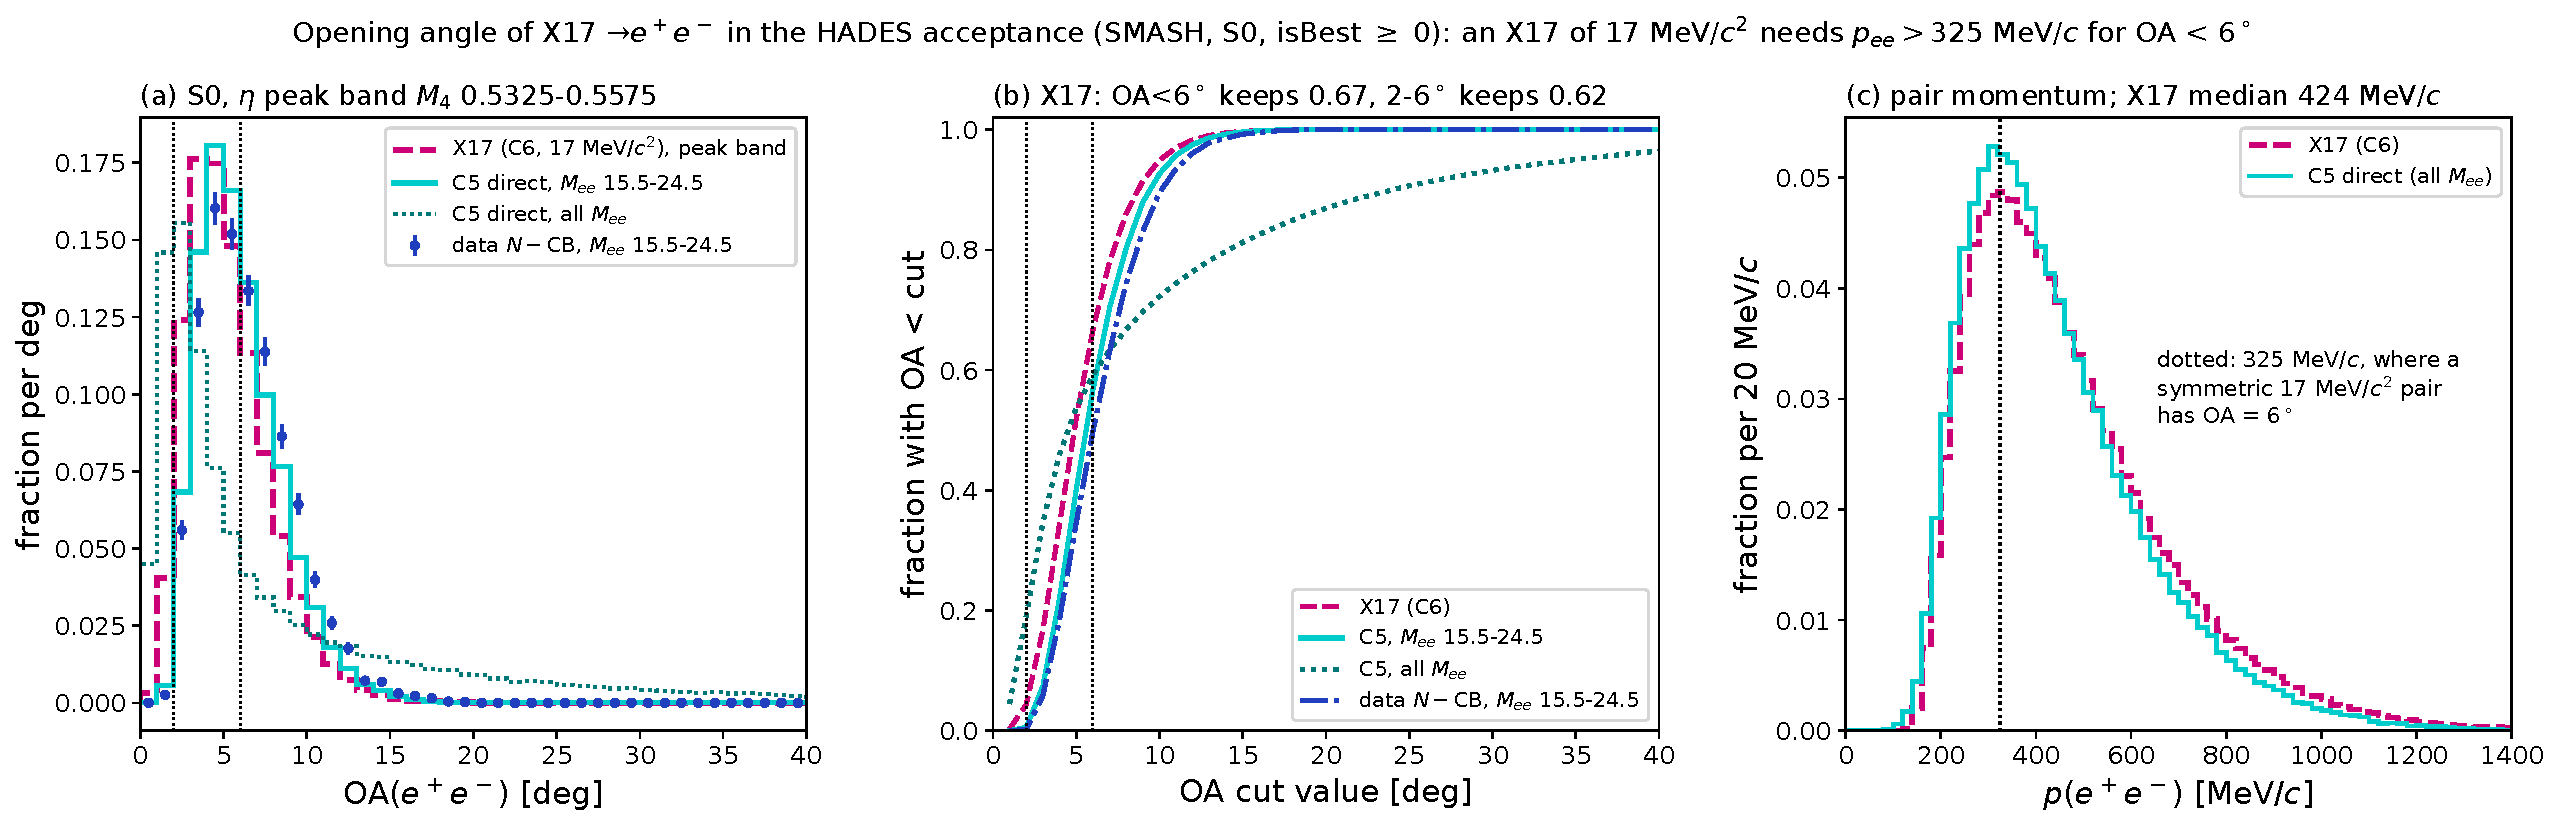
\includegraphics[width=\textwidth]{figs_all/e1_x17_oa_v2.pdf}
\caption{\textbf{What it shows: two thirds of a simulated X17 has OA$<6^\circ$, but the direct decays and the data of the same pair mass have the same opening angles.}
Selection: SMASH and data with S0 (PT3 trigger, event vertex in the target region ($\vz>-160$\,mm), \betanew particle identification (pions within $3\sigma$, leptons within $5\sigma$ and with a RICH ring), energy-loss-corrected momenta of all four tracks, all stored combinations of each event (isBest $\ge0$), both pions in the event-vertex fit); the $\eta$ peak band \Mfour 0.5325--0.5575\,\GeVcc; X17 window \Mee 15.5--24.5\,\MeVcc; OA 0--40$^\circ$ in 1$^\circ$ bins, pair momentum 0--1400\,\MeVc in 20\,\MeVc bins; X17: simulated $\eta\to\pipi X17$, $X17\to\ee$ at 17.000\,\MeVcc (C6); C5: the direct decays of SMASH (mode A, $w\times$V3, $M_4'=0.99615\,M_4$); data: $N-\mathrm{CB}$, CB $=2\sqrt{N_{++}N_{--}}$ of the like-sign data with the same cuts (10\,\MeVcc cells of \Mfour, $k=1$), shared out to the OA bins by the like-sign share of each 50\,\MeVcc band.
Opening angle of X17$\to\ee$ in the HADES acceptance (SMASH, S0, isBest $\ge0$, $\eta$ peak band \Mfour 0.5325--0.5575\,\GeVcc). (a) OA
distributions normalised to unit area: X17 (C6, 17.000\,\MeVcc, dashed magenta), the direct decays C5 in the X17 window \Mee 15.5--24.5\,\MeVcc
(cyan) and at all \Mee (dotted), the data $N-\mathrm{CB}$ in the X17 window (blue). (b) Fraction below an OA cut: OA$<6^\circ$ keeps 0.67 of the
X17, $2^\circ<$OA$<6^\circ$ 0.62. (c) Pair momentum of the X17 and of C5 (X17 median 424\,\MeVc); dotted: 325\,\MeVc, below which a
17\,\MeVcc pair cannot have OA$<6^\circ$. Redrawn (\code{e1_x17_oa_v2.pdf}) with the median of panel (c) corrected by the verifier (the e1
figure prints 414\,\MeVc, a binning artefact).}
\label{fig:e1-x17oa}
\end{figure}

\begin{table}[htbp]
\centering
\caption{\textbf{What it shows: in the X17 window the X17, the direct decays and the data have OA$<6^\circ$ equally often (50--58\,\%).}
Fractions of the opening-angle distribution, SMASH and data, selection S0, $\eta$ peak band (\Mfour 0.5325--0.5575\,\GeVcc); X17 window: \Mee
15.5--24.5\,\MeVcc. Mean: over 0--40$^\circ$. X17 pair momentum (peak band): median 424\,\MeVc (420 in the X17 window); 0.727 of the pairs above
325\,\MeVc (0.719 in the window). Source: \code{tables_all/e1_table.txt}, section~5; momentum from the verification e1v.}
\label{tab:e1oaf}
\small
\begin{tabular}{@{}l r r r r r@{}}
\toprule
distribution & OA$<2^\circ$ & $2$--$6^\circ$ & OA$<6^\circ$ & OA$>6^\circ$ & mean OA [$^\circ$] \\
\midrule
X17 (C6), peak band & 0.044 & 0.623 & 0.666 & 0.334 & 5.3 \\
X17 (C6), X17 window & 0.009 & 0.571 & 0.581 & 0.419 & 5.9 \\
direct decays C5, peak band (all \Mee) & 0.191 & 0.401 & 0.592 & 0.408 & 7.7 \\
direct decays C5, X17 window & 0.006 & 0.561 & 0.567 & 0.433 & 6.0 \\
data $N-\mathrm{CB}$, peak band & 0.242 & 0.523 & 0.765 & 0.235 & 5.3 \\
data $N-\mathrm{CB}$, X17 window & 0.003 & 0.495 & 0.497 & 0.503 & 6.5 \\
\bottomrule
\end{tabular}
\end{table}

\begin{figure}[tbp]
\centering
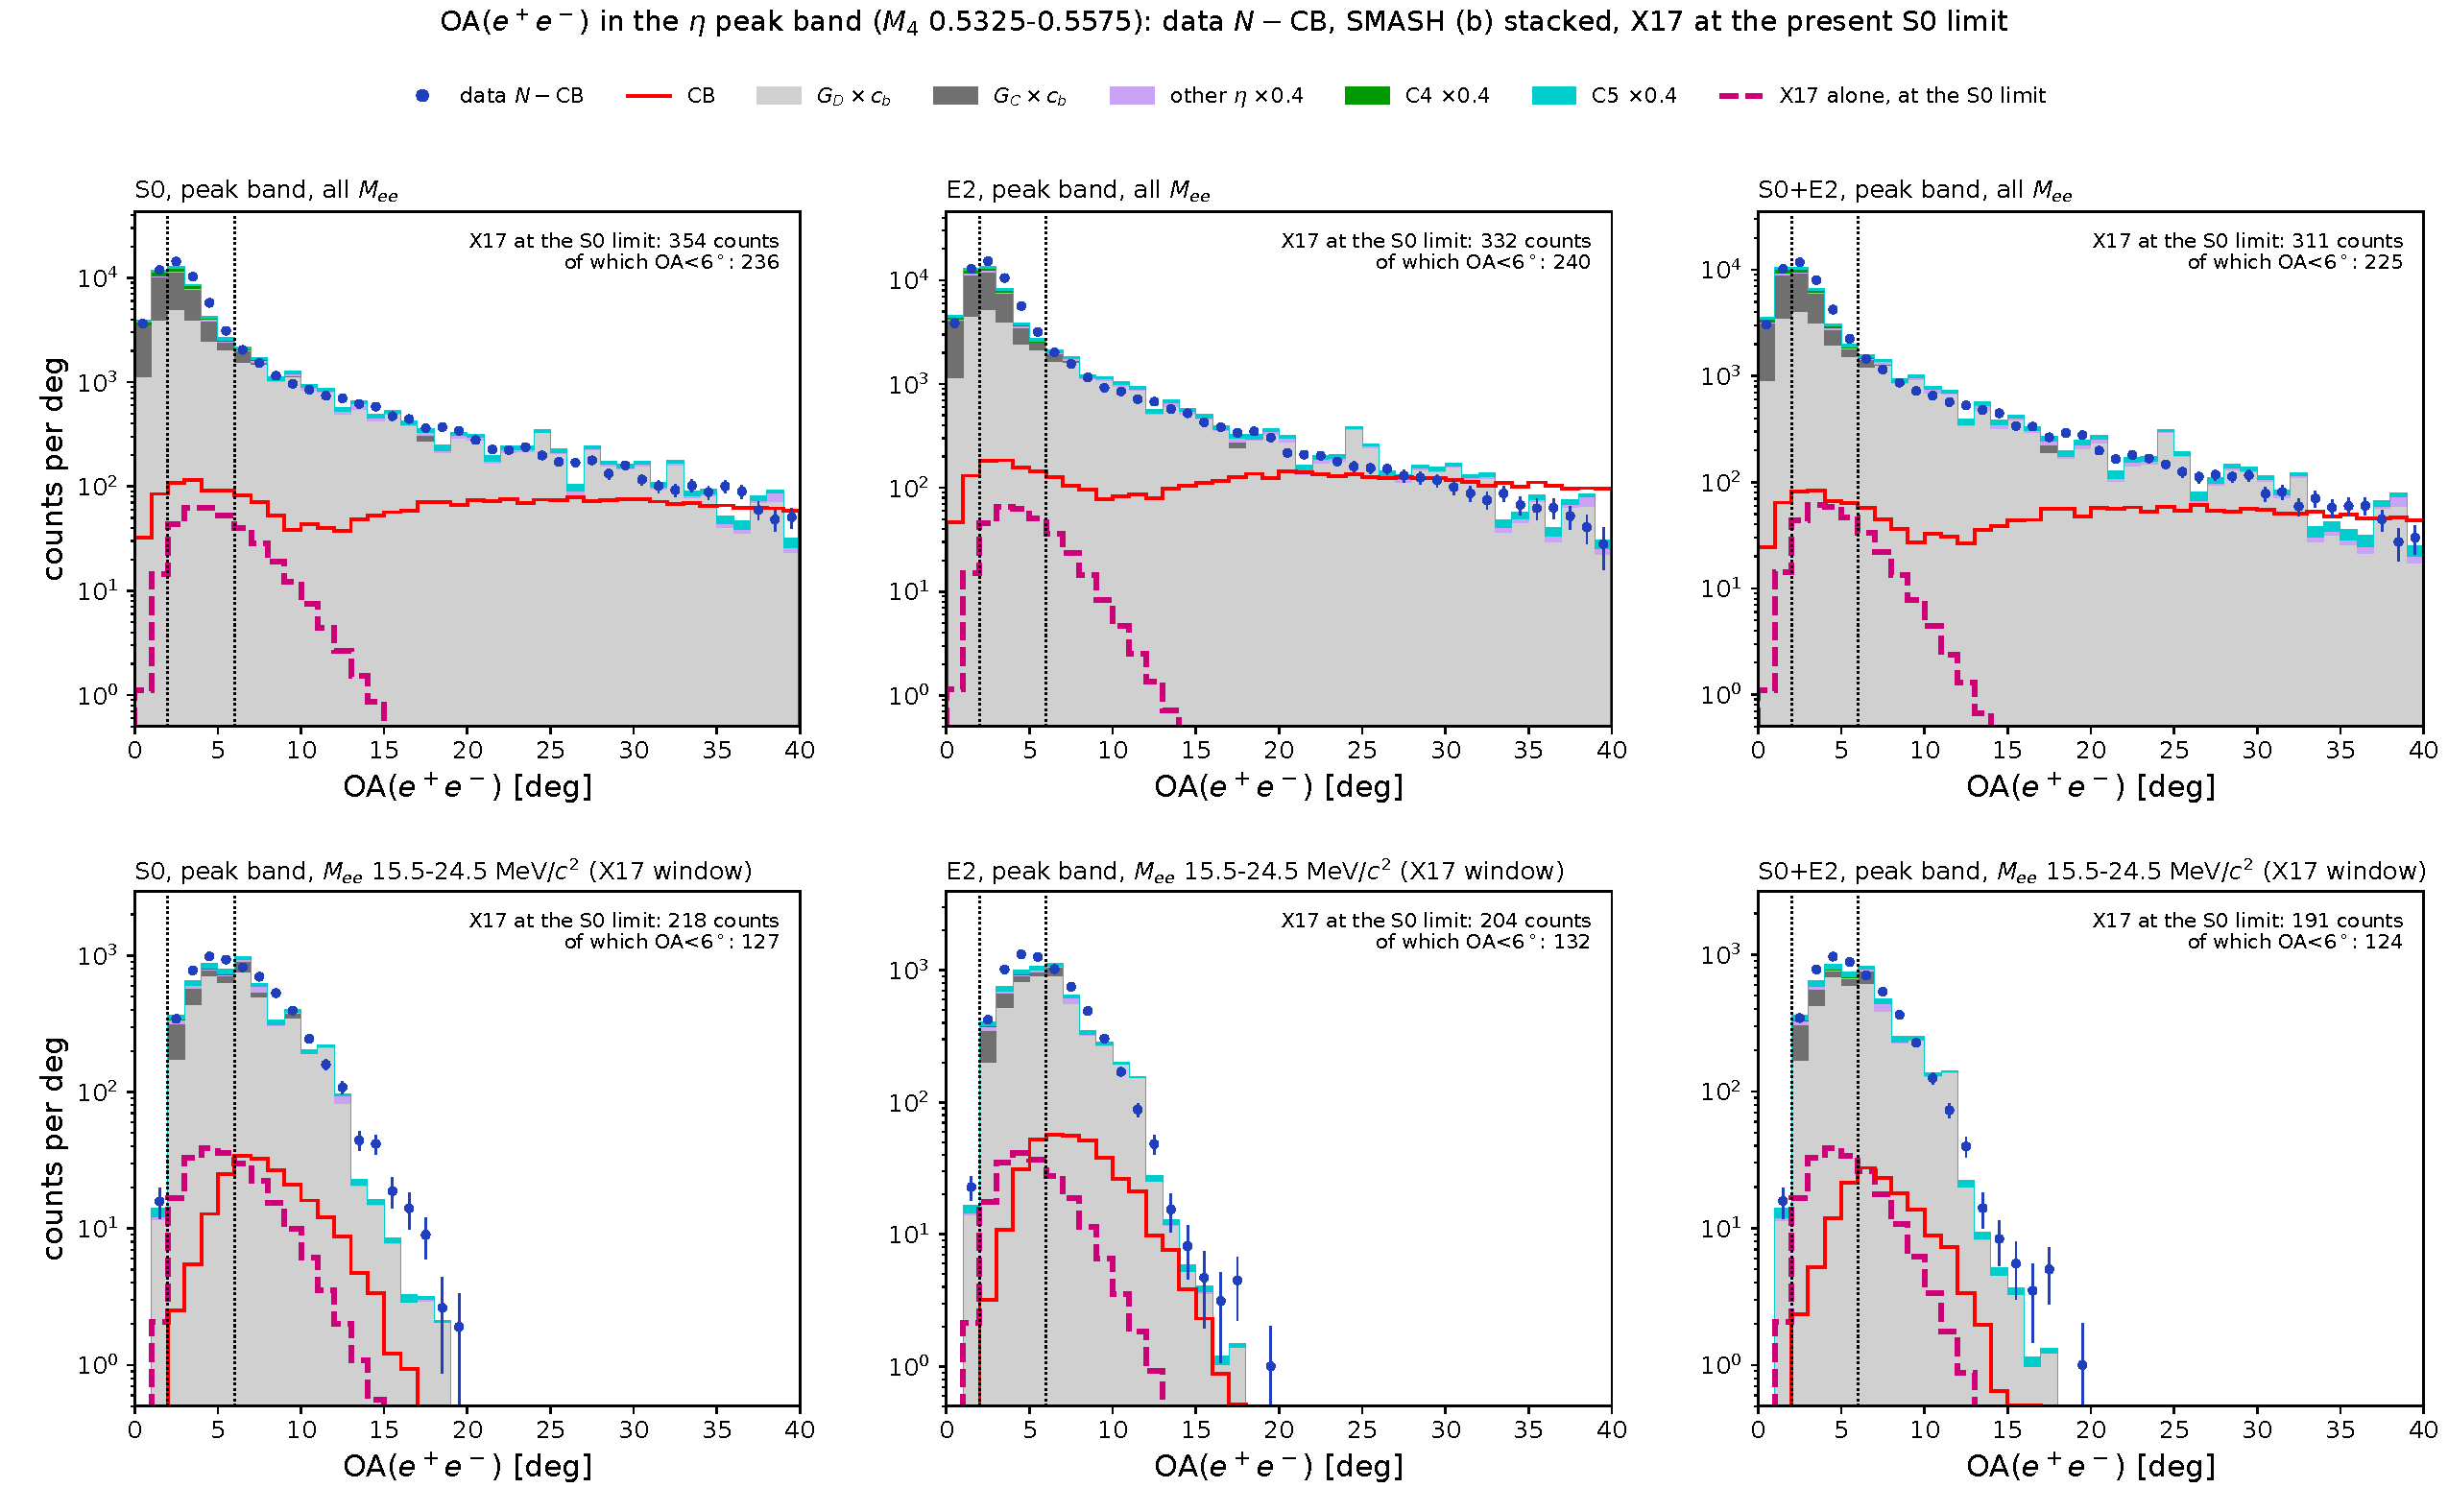
\includegraphics[width=\textwidth]{figs_all/e1_oa_cnt.pdf}
\caption{\textbf{What it shows: in the peak band the data follow the scaled SMASH in OA (in the X17 window up to about $12^\circ$); an X17 at the limit is a few per cent of the counts.}
Selection: data and SMASH in the $\eta$ peak band \Mfour 0.5325--0.5575\,\GeVcc, OA 0--40$^\circ$ in 1$^\circ$ bins; left column S0 (PT3 trigger, event vertex in the target region ($\vz>-160$\,mm), \betanew particle identification (pions within $3\sigma$, leptons within $5\sigma$ and with a RICH ring), energy-loss-corrected momenta of all four tracks, all stored combinations of each event (isBest $\ge0$), both pions in the event-vertex fit); middle column ``pre'' (the same without the pion-vertex requirement) + $\alpha_{\mathrm{lab}}<50^\circ$, $\alpha_\eta>140^\circ$, \Mpipi$<0.46$\,\GeVcc (\cs{E2}; $\alpha_{\mathrm{lab}}$, $\alpha_\eta$: angle between the \pipi and \ee systems in the laboratory, in the $\eta$ rest frame; OA: \ee opening angle); right column S0 + the same three cuts; top row all \Mee, bottom row \Mee 15.5--24.5\,\MeVcc. CB $=2\sqrt{N_{++}N_{--}}$ of the like-sign data with the same cuts (10\,\MeVcc cells of \Mfour, $k=1$), shared out to the OA bins by the like-sign share of each 50\,\MeVcc band. SMASH p+p at 4.5\,GeV (standard, lepton and $\eta$ sets, mode A) at its cross sections $\times$ PDG BR $\times$ the $\eta$-decay weights V3, masses moved to the data scale ($M_4'=0.99615\,M_4$, $\Mpipi'=0.9952\,\Mpipi$), same cuts (\Mpipi cut on $\Mpipi'$), shown as display (b): $\eta$ channels $\times0.40$, non-$\eta$ background $\times c_b$ from the data in \Mfour 0.575--0.70\,\GeVcc (all \Mee and \Mpipi, one factor per selection). X17: simulated C6 (17\,\MeVcc) at the S0 limit, 392 counts in \Mfour 0.5225--0.6100\,\GeVcc, times the simulated X17 efficiency of the selection.
OA$(\ee)$ in the $\eta$ peak band (\Mfour 0.5325--0.5575\,\GeVcc), 1$^\circ$ bins, counts per degree, log scale. Columns: S0; \cs{E2} (``pre''
base: the kinematic cuts of the slides without OA); S0\,+\,\cs{E2}. Top: all \Mee; bottom: the X17 window \Mee 15.5--24.5\,\MeVcc. Blue: data
$N-\mathrm{CB}$; red line: CB; stack: SMASH (b) ($G_D$, $G_C$ $\times c_b$ greys; other $\eta$ violet, C4 green, C5 cyan, $\times0.4$); dashed
magenta: the X17 alone at the present S0 limit (392 counts in the X2D range, scaled by the simulated X17 efficiency of the selection). The box gives
the X17 counts at the limit and those with OA$<6^\circ$ (S0, X17 window: 218 and 127). Dotted: $2^\circ$ and $6^\circ$.}
\label{fig:e1-oa}
\end{figure}

\subsection{What the cuts do for an X17 search}
\label{sec:e1x17}
\begin{table}[!htb]
\centering
\caption{\textbf{What it shows: in the X17 window S0 alone has the best counting proxy; OA$<6^\circ$ raises S/B but loses 42\,\% of the X17.}
X17 window (\Mfour 0.5325--0.5575\,\GeVcc, \Mee 15.5--24.5\,\MeVcc), 22 selections. $\varepsilon_X/\varepsilon_X(\mathrm{S0})$: simulated X17
efficiency (C6) relative to S0; $N$, CB: data counts; $N_X$: X17 counts of an X17 at the present S0 limit (392 counts in the X2D range) seen through the
selection; $Z=N_X/\sqrt{N+\mathrm{var\,CB}}$; proxy $=\sqrt{N}/(\varepsilon_X/\varepsilon_X(\mathrm{S0}))/\sqrt{N_{\mathrm{S0}}}$ (smaller is
better); S/B gain $=(\varepsilon_X/\varepsilon_X(\mathrm{S0}))/(N/N_{\mathrm{S0}})$. Counting estimates, not the frozen likelihood; the CB of the
OA$<6^\circ$ selections is a lower limit. Cut names in roman. Source: \code{tables_all/e1_tableX.tex}.}
\label{tab:e1X}
{\footnotesize\setlength{\tabcolsep}{4pt}\renewcommand{\arraystretch}{1.0}
\tabin{e1_tableX.tex}\par}
\end{table}

Table~\ref{tab:e1X} and Fig.~\ref{fig:e1-sens} give, per selection, what is kept in the X17 window; Fig.~\ref{fig:e1-mee} shows the \Mee
spectrum of the peak band with the X17 line at the present limit.
\begin{itemize}\setlength{\itemsep}{1pt}
\item \textbf{The cuts act on the X17 as on the direct decays.} In every selection the simulated X17 efficiency follows that of the direct decays C5
      within 5\,\% (relative to S0). A cut cannot prefer the X17 over the direct decays $\eta\to\ppee$, its companion in the peak band.
\item \textbf{The kinematic cuts on S0} keep 75--90\,\% of the X17 and 71--84\,\% of the data counts in the window. S/B improves by 5--7\,\%, but
      the counting proxy is 1.02--1.04 (\cs{E4}, \cs{E4oa}, \cs{E2}, \cs{E1}) and 1.11--1.12 with \Mpipi$<0.42$ (\cs{E3}, \cs{E3oa}): worse than S0.
\item \textbf{OA$<6^\circ$ on S0} keeps 51--58\,\% of the X17 and 44--49\,\% of the counts. S/B improves by 17--19\,\%, but the proxy is 1.20--1.29
      (\cs{X3} 1.20, S0\,+\,\cs{X1} 1.21, S0\,+\,\cs{X2} 1.23, S0\,+\,\cs{X2old} 1.29).
\item \textbf{Every selection on the ``pre'' base} is worse than S0 (proxy 1.12--1.42): without the pion-vertex cut the window holds 44\,\% more counts,
      but only 7.5\,\% more X17.
\item \textbf{An X17 at the present limit} (218 counts in the S0 window) would be a counting excess of $Z=2.72$ in S0, 2.61 and 2.63 after
      S0\,+\,\cs{E1} and S0\,+\,\cs{E2}, 2.11--2.27 after OA$<6^\circ$ on S0, and 1.93--2.07 with OA$<6^\circ$ on the ``pre'' base. No cut makes it
      more visible. OA$<6^\circ$ would help only if the background systematics dominated (S/B $+19$\,\%), and it costs 42\,\% of the signal.
\item \textbf{SMASH cannot be the X17 background model.} In the peak band the scaled SMASH misses the \Mee shape by 10--25\,\%: data/(CB +
      model) is 1.02--1.24 below 25\,\MeVcc (S0: 1.125 at 2--14, 1.086 at 15.5--24.5\,\MeVcc) and 0.78--0.90 at 26--62\,\MeVcc (S0 0.877), while an
      X17 at the present limit is only 3--5\,\% of CB + model in the window (S0 3.7\,\%). This is why the frozen X17 fit measures the background
      in every \Mee row from the \Mfour side bands instead of taking it from SMASH (\S\ref{sec:x17}); the cuts do not change it.
\end{itemize}

\begin{figure}[tbp]
\centering
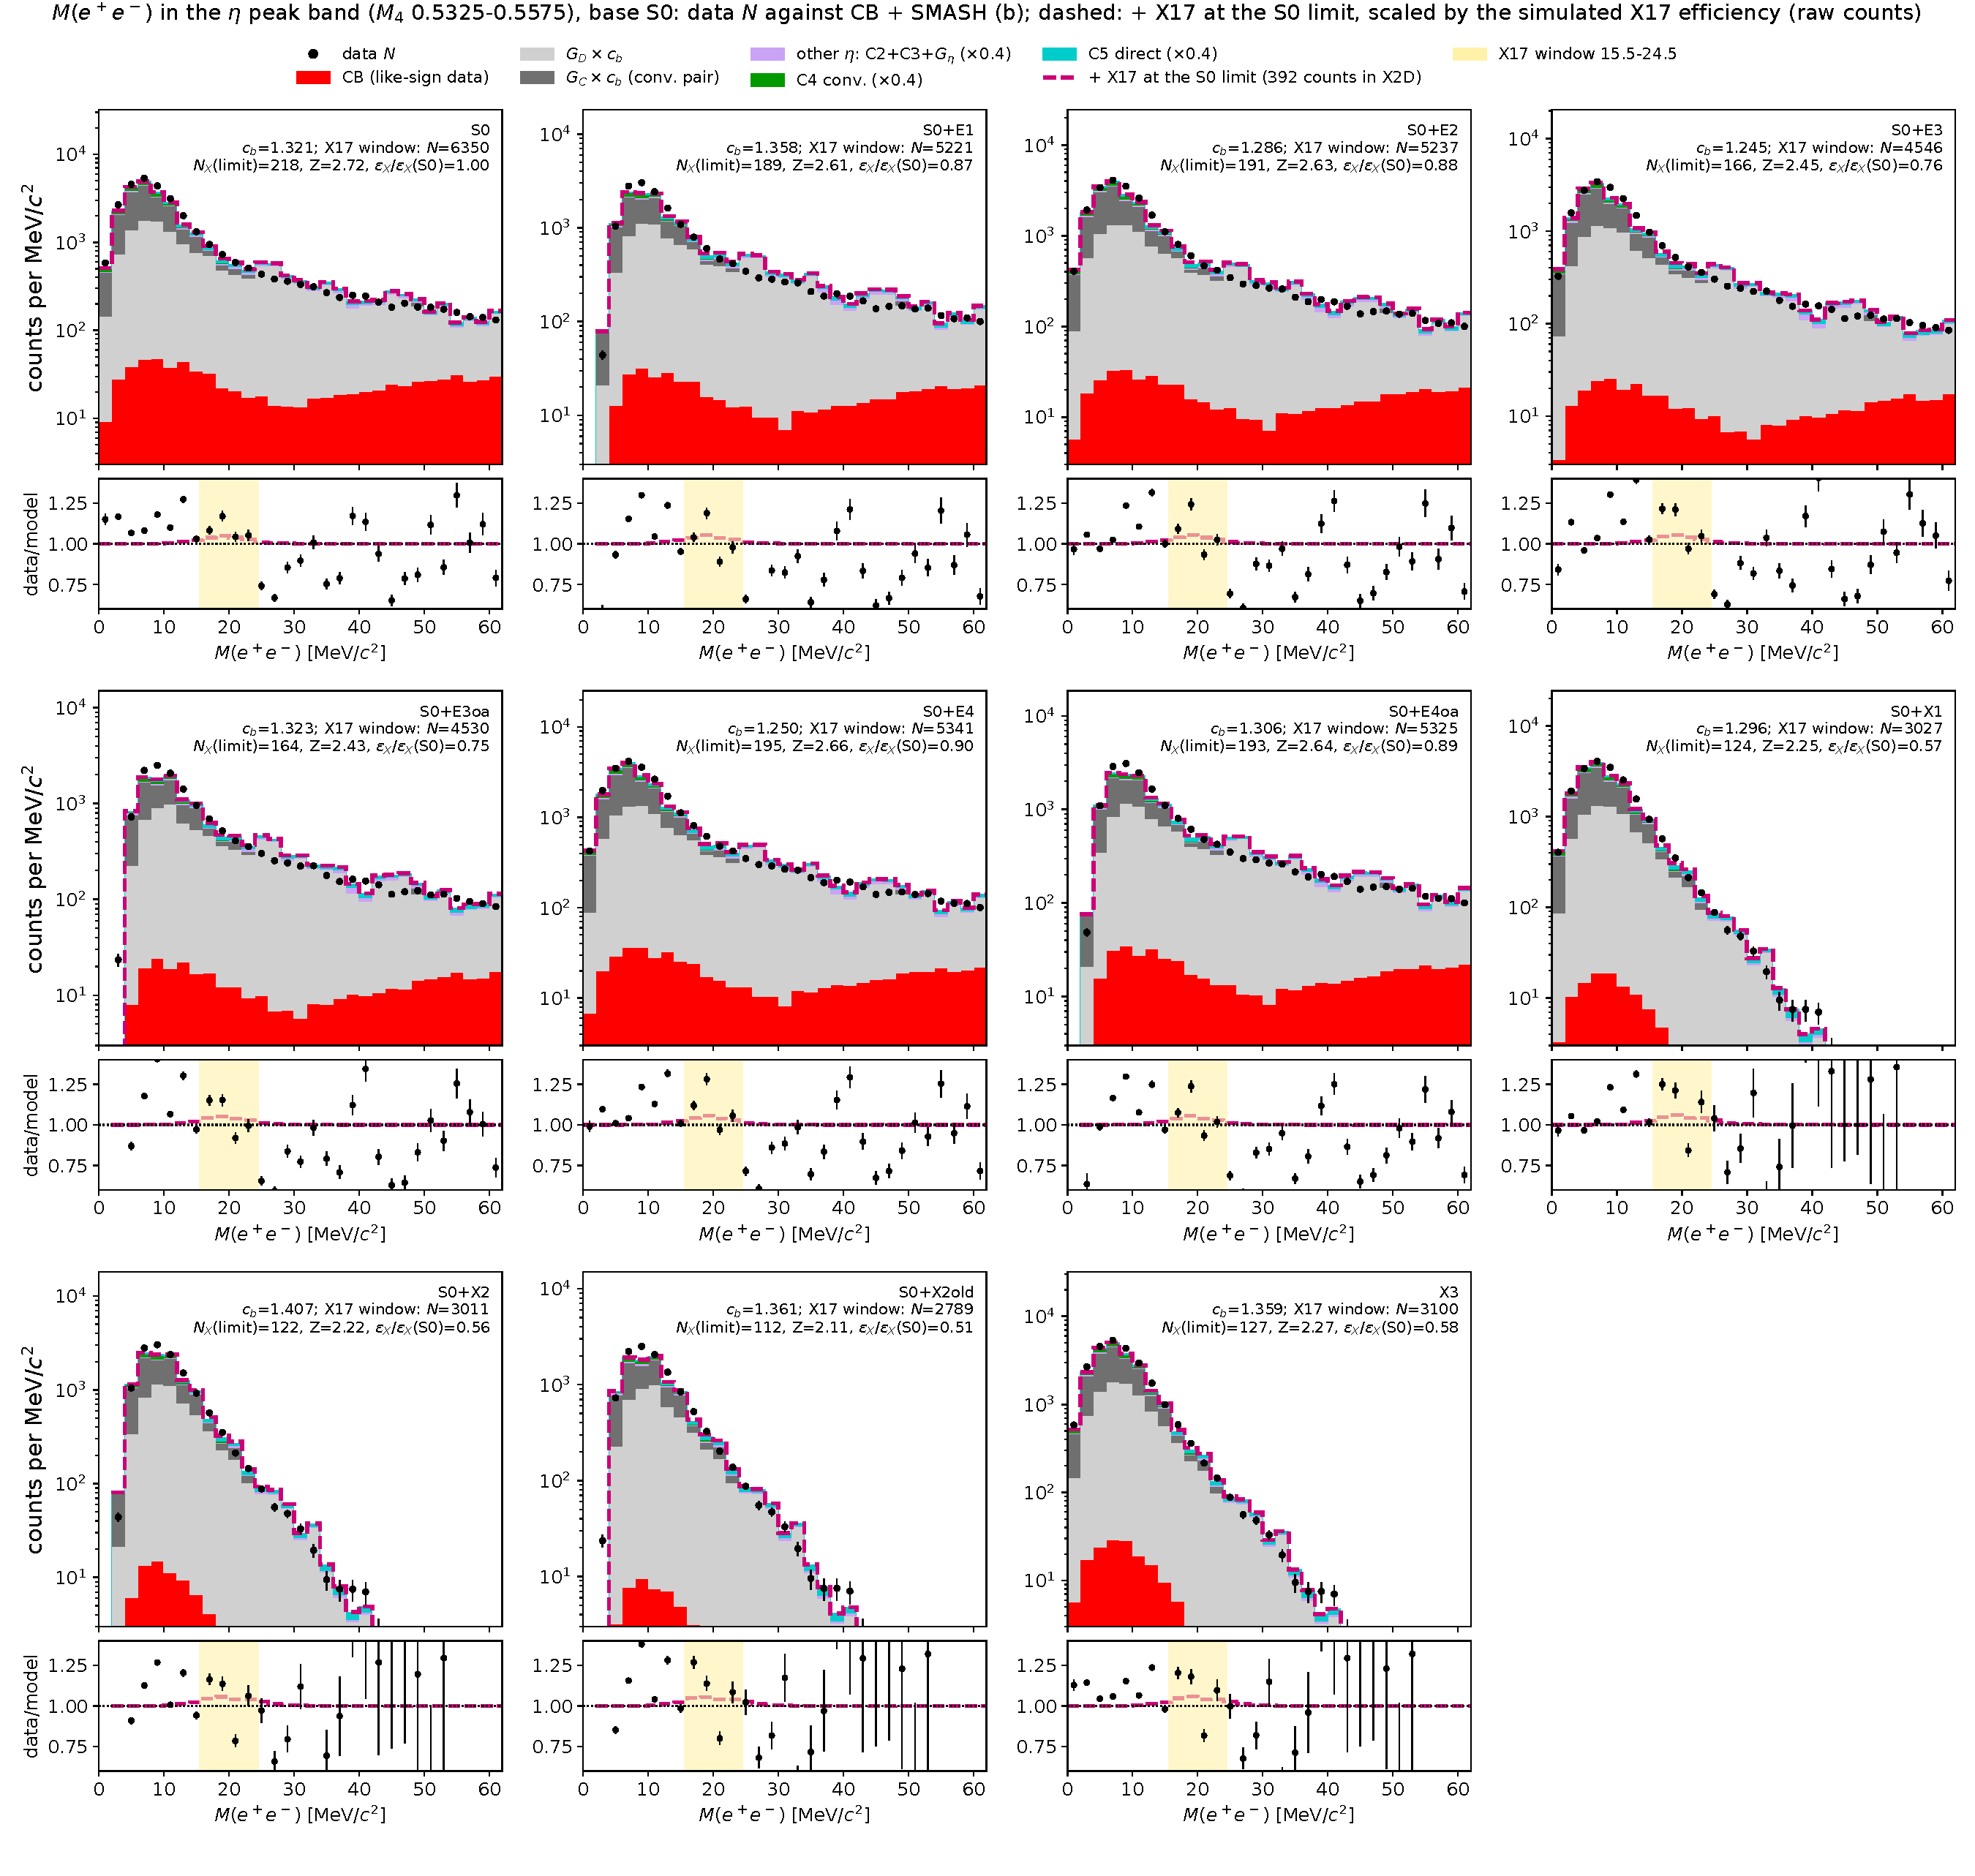
\includegraphics[width=0.98\textwidth]{figs_all/e1_mee_S0_v2_cnt.pdf}
\caption{\textbf{What it shows: in the peak band the scaled SMASH misses the \Mee shape by 10--25\,\%, more than an X17 at the limit would add.}
Selection: data and SMASH in the $\eta$ peak band \Mfour 0.5325--0.5575\,\GeVcc, \Mee 0--62\,\MeVcc in 2\,\MeVcc bins; first panel S0 (PT3 trigger, event vertex at $\vz>-160$\,mm, \betanew identification, corrected momenta, isBest $\ge0$, both pions in the event-vertex fit), then S0 + one cut set each, with $A$: $\alpha_{\mathrm{lab}}<50^\circ$ and $\alpha_\eta>140^\circ$ (angle between the \pipi and \ee systems in the laboratory, in the $\eta$ rest frame) and OA the \ee opening angle: \cs{E1}: $A$, \Mpipi$<0.46$\,\GeVcc, OA$>2^\circ$; \cs{E2}: $A$, \Mpipi$<0.46$\,\GeVcc; \cs{E3}: $A$, \Mpipi$<0.42$\,\GeVcc; \cs{E3oa}: \cs{E3}, OA$>2^\circ$; \cs{E4}: $A$; \cs{E4oa}: $A$, OA$>2^\circ$; \cs{X1}: \cs{E2}, OA$<6^\circ$; \cs{X2}: \cs{E2}, $2^\circ<$OA$<6^\circ$; \cs{X2old}: \cs{E3}, $2^\circ<$OA$<6^\circ$; OA$<6^\circ$ alone (\cs{X3}). CB from the like-sign data (10\,\MeVcc cells, $k=1$, shared out by the like-sign share of each 50\,\MeVcc band); SMASH (mode A, $\sigma\times$PDG BR$\times$V3, $M_4'=0.99615\,M_4$, $\Mpipi'=0.9952\,\Mpipi$; same cuts) as display (b), $c_b$ from \Mfour 0.575--0.70\,\GeVcc; X17 (C6) at the S0 limit, 392 counts in \Mfour 0.5225--0.6100\,\GeVcc.
\Mee in the $\eta$ peak band (\Mfour 0.5325--0.5575\,\GeVcc), 2\,\MeVcc bins, counts per \MeVcc, log scale; S0 and the ten cut selections on S0.
Black: data $N$. Stack: CB from the like-sign data (red; spread by the like-sign share of each \Mee bin in its 50\,\MeVcc \Mfour band), $G_D\times
c_b$ (light grey), $G_C\times c_b$ (dark grey), other $\eta$ C2+C3+\Geta (violet), C4 (green) and C5 (cyan), every $\eta$ term $\times0.4$.
Dashed magenta: the same plus the simulated X17 (17\,\MeVcc) at the present S0 limit (392 raw counts in the X2D range), scaled to each selection by
its simulated X17 efficiency. Lower pads: data/(CB + model); dashed: (CB + model + X17)/(CB + model); yellow: the X17 window 15.5--24.5\,\MeVcc.
The panel text gives $c_b$, $N$ in the X17 window, the X17 counts at the limit $N_X$, $Z$ and $\varepsilon_X/\varepsilon_X(\mathrm{S0})$. The SMASH
templates have few simulated entries here (\S\ref{sec:e1cav}). The same for the ``pre'' base: \code{figs_all/e1_mee_pre_v2_cnt.pdf}.}
\label{fig:e1-mee}
\end{figure}

\begin{figure}[tbp]
\centering
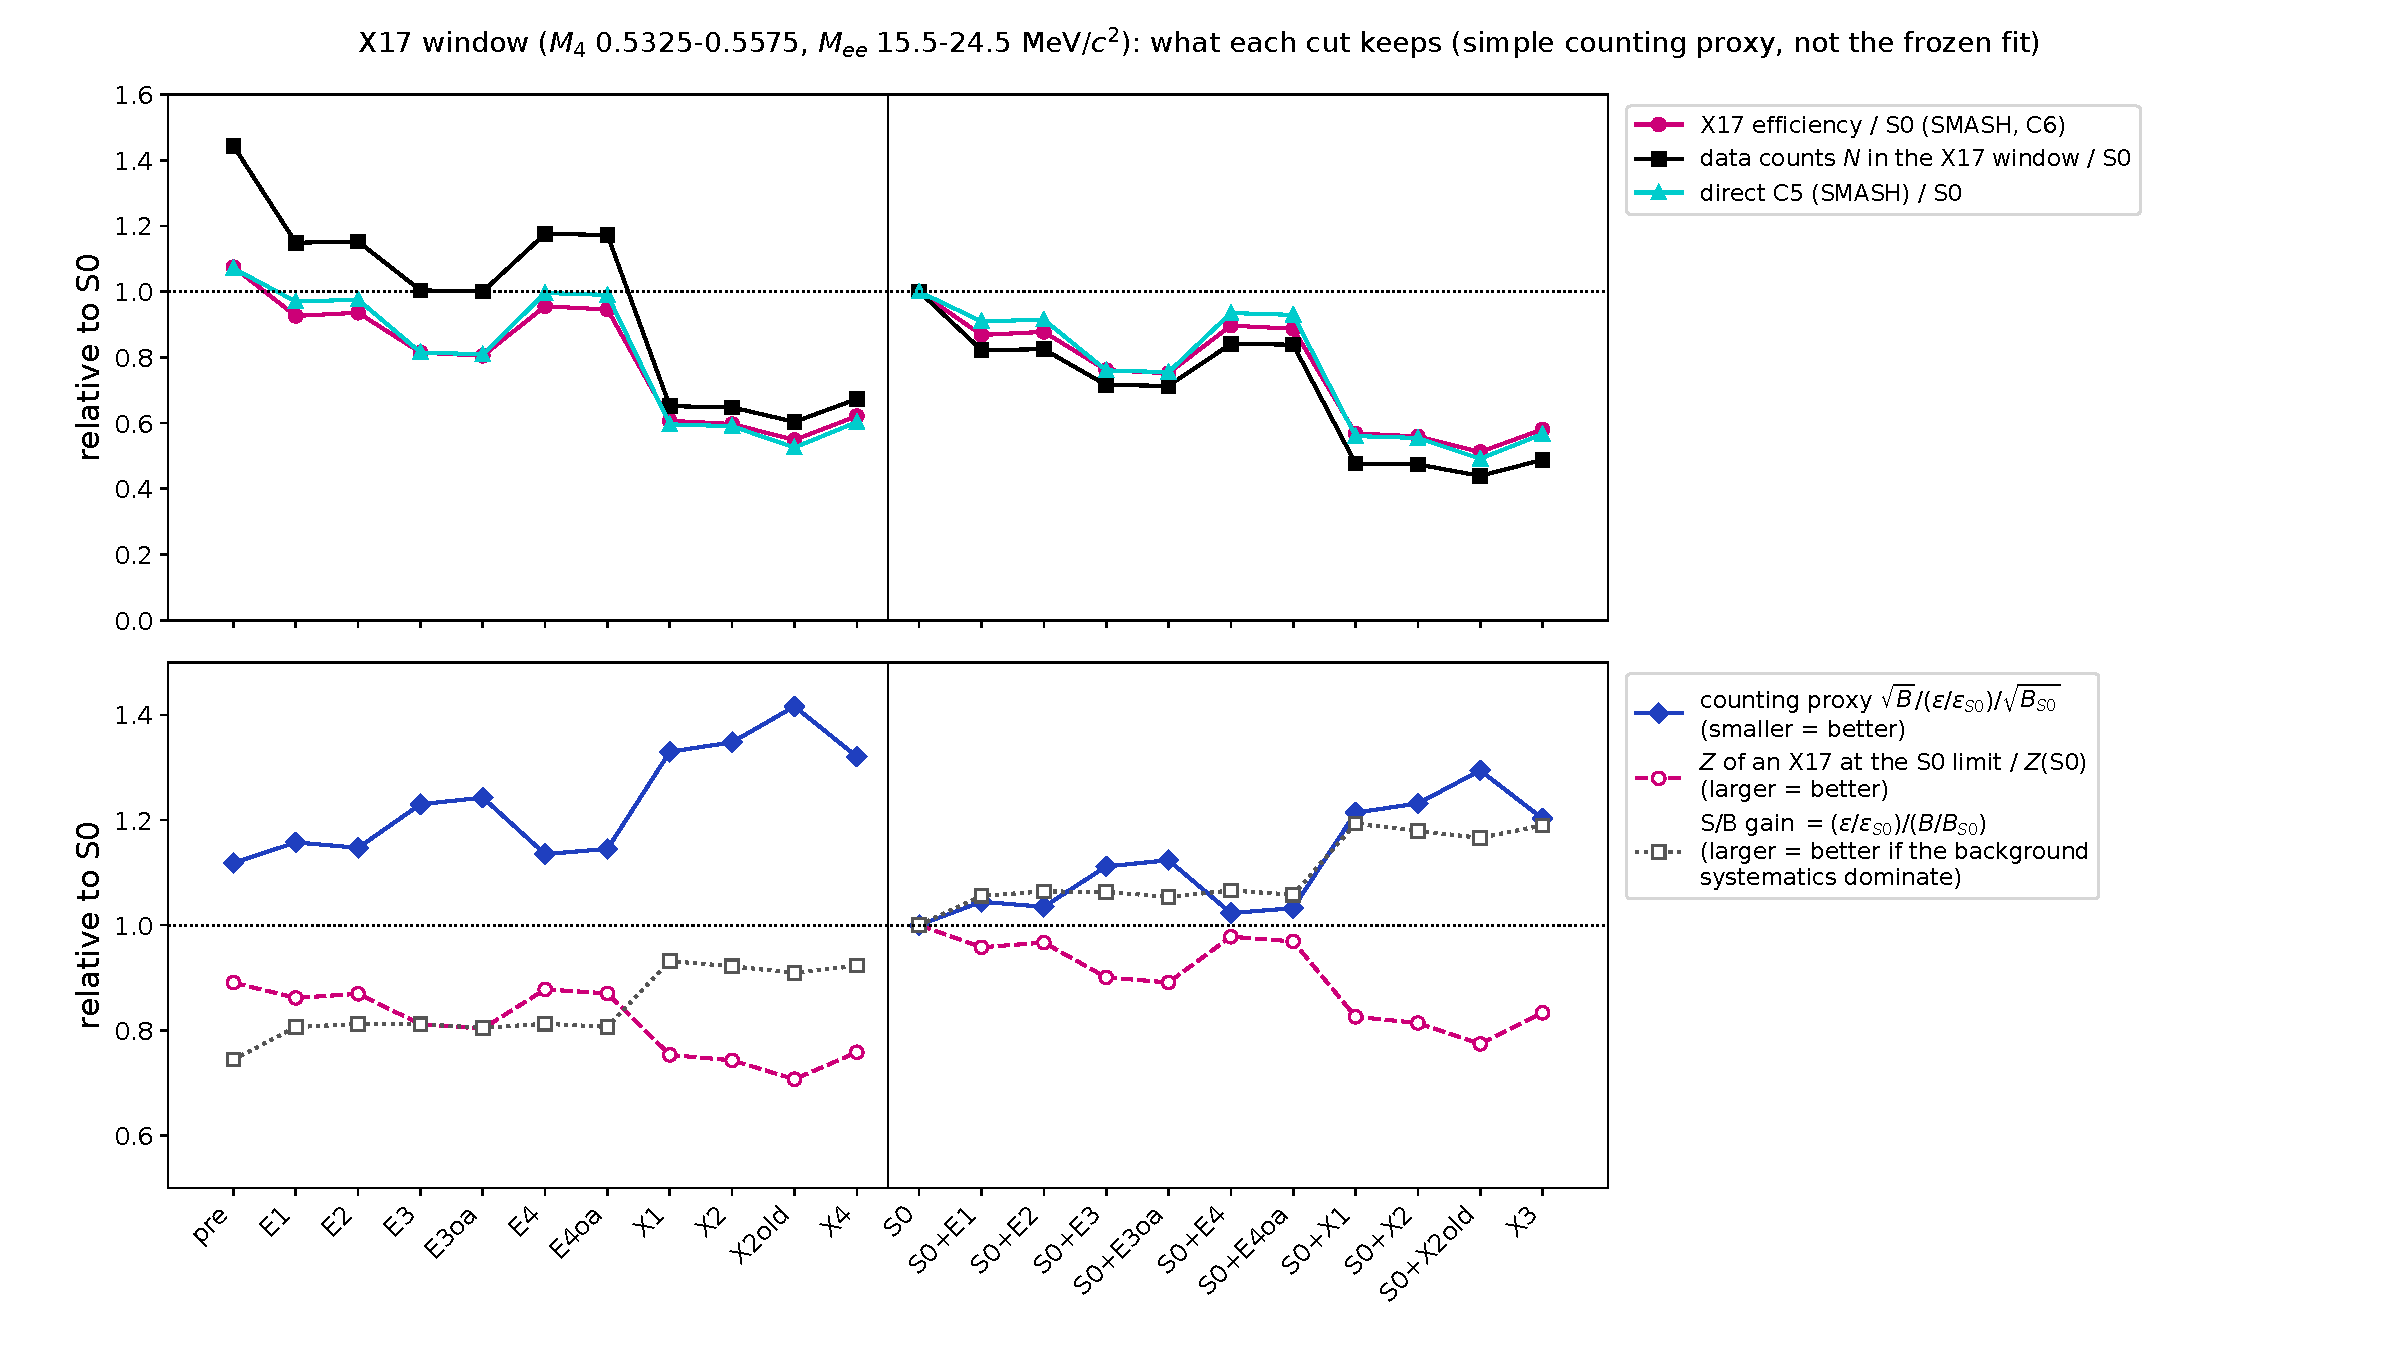
\includegraphics[width=0.86\textwidth]{figs_all/e1_x17_sens_v2_cnt.pdf}
\captionof{figure}{\textbf{What it shows: no cut makes an X17 easier to see in a simple count than S0 alone; the cuts act on the X17 as on the direct decays.}
Selection: data and SMASH in the X17 window \Mfour 0.5325--0.5575\,\GeVcc and \Mee 15.5--24.5\,\MeVcc; left block ``pre'' (PT3 trigger, event vertex in the target region ($\vz>-160$\,mm), \betanew particle identification (pions within $3\sigma$, leptons within $5\sigma$ and with a RICH ring), energy-loss-corrected momenta of all four tracks, all stored combinations of each event (isBest $\ge0$)), right block S0 (``pre'' + both pions in the event-vertex fit), each alone and with one cut set, with $A$: $\alpha_{\mathrm{lab}}<50^\circ$ and $\alpha_\eta>140^\circ$ (angle between the \pipi and \ee systems in the laboratory, in the $\eta$ rest frame) and OA the \ee opening angle: \cs{E1}: $A$, \Mpipi$<0.46$\,\GeVcc, OA$>2^\circ$; \cs{E2}: $A$, \Mpipi$<0.46$\,\GeVcc; \cs{E3}: $A$, \Mpipi$<0.42$\,\GeVcc; \cs{E3oa}: \cs{E3}, OA$>2^\circ$; \cs{E4}: $A$; \cs{E4oa}: $A$, OA$>2^\circ$; \cs{X1}: \cs{E2}, OA$<6^\circ$; \cs{X2}: \cs{E2}, $2^\circ<$OA$<6^\circ$; \cs{X2old}: \cs{E3}, $2^\circ<$OA$<6^\circ$; OA$<6^\circ$ alone (\cs{X4}, \cs{X3}). Data: counts $N$ in the window and CB $=2\sqrt{N_{++}N_{--}}$ of the like-sign data with the same cuts (10\,\MeVcc cells of \Mfour, $k=1$), shared out by the like-sign share of each 50\,\MeVcc band. SMASH: X17 (C6, 17\,\MeVcc) and direct decays C5 of SMASH p+p at 4.5\,GeV (standard, lepton and $\eta$ sets, mode A) at its cross sections $\times$ PDG BR $\times$ the $\eta$-decay weights V3, masses moved to the data scale ($M_4'=0.99615\,M_4$, $\Mpipi'=0.9952\,\Mpipi$), same cuts (\Mpipi cut on $\Mpipi'$). X17: simulated C6 (17\,\MeVcc) at the S0 limit, 392 counts in \Mfour 0.5225--0.6100\,\GeVcc, times the simulated X17 efficiency of the selection.
X17 window (\Mfour 0.5325--0.5575\,\GeVcc, \Mee 15.5--24.5\,\MeVcc), per selection, relative to S0 (left block: ``pre'' base, right: S0 base).
Top: X17 efficiency (SMASH C6, magenta), the direct decays C5 (cyan) and the data counts $N$ (black). Bottom: the counting proxy (blue, smaller is
better), $Z$ of an X17 at the present limit relative to S0 (magenta, larger is better) and the S/B gain (grey; larger is better only if the
background systematics dominate). A counting estimate, not the frozen likelihood. Redrawn (\code{e1_x17_sens_v2.pdf}) without lines across the
divider of the two bases.}
\label{fig:e1-sens}
\end{figure}

\subsection{The approach of the earlier analysis: integral scaling, a three-scale fit and side bands (linear scale)}
\label{sec:e1prev}
\inshort{drawn as in the earlier analysis, with SMASH scaled to the data integral, SMASH gets the total right by construction but the parts
wrong: it is about 20\,\% too high in the bump and about 10\,\% too low just above the peak ($\chi^2/\mathrm{ndf}=5.8$ in 0.40--0.70\,\GeVcc).
With our measured scales it describes the data up to 0.70\,\GeVcc ($\chi^2/\mathrm{ndf}=2.1$). The $\eta$ scales of the three-scale global fit
move with the treatment of the SMASH templates by 7--20 times their statistical errors, and the \Mee side-band view cannot test X17. The best
combination only (isBest $=1$) gives the same picture. A demonstration with the background fixed on the slope and two free $\eta$ scales (not
a measurement) puts the bump at $0.455\pm0.049$ and the peak at $0.65\pm0.13$ of SMASH; both move with the assumed background shape.
Converted with the report's chain, these scales give \sigeta$=0.47$\,mb (bump) and 0.67\,mb (peak) against 0.444 and 0.429\,mb measured,
and a one-window X17 count in the earlier style gives limits of $(5$--$8)\times10^{-5}$ that move between 1.6 and $13\times10^{-5}$ with the
side-band normalisation and the $\eta$ scale (frozen limit $3.16\times10^{-5}$).}

At the analyst's request the data and SMASH after the typical cuts (``pre'' + \cs{E1}) are also shown in the style of the approach of the earlier
analysis presented at HADES collaboration meetings: linear \Mfour spectra with SMASH scaled to the data integral and the four $\eta$ decays drawn
as separate lines (Fig.~\ref{fig:e1-prev-m4}), a three-scale global fit (Fig.~\ref{fig:e1-prev-gfit}), and the \Mee spectrum of the $\eta$-peak
window minus the side bands (Fig.~\ref{fig:e1-prev-mee}). Table~\ref{tab:e1prev} gives the numbers. All stored combinations (isBest $\ge0$) are
the nominal choice of this analysis and are drawn first. The best combination only (isBest $=1$, in the data and in SMASH) is drawn only to
reproduce the approach of the earlier slides; it is not an alternative result. In both cases the CB comes from the like-sign data; the simulation
never provides it. None of these numbers is used elsewhere in this report.

\textbf{What was done} (package prevstyle).
\begin{enumerate}\setlength{\itemsep}{1pt}
\item \textbf{Data.} The counts $N$ and the like-sign counts with the same cuts; CB $=2\sqrt{N_{++}N_{--}}$ in 10\,\MeVcc cells of \Mfour,
      interpolated to 2.5\,\MeVcc, $k=1$; in the \Mee bins of a window the CB is shared out by the like-sign share of each bin in its 50\,\MeVcc
      band. Errors: event groups for $N$, 200 replicas for the CB. For isBest $=1$ the CB is the naive formula $2\sqrt{N_{++}N_{--}}$ of the best
      like-sign combinations, as in the earlier analysis.
\item \textbf{SMASH} as in \S\ref{sec:e1proc}, in expected counts ($\sigma\times L\times63/64$); the Dalitz pairs of $\eta\to\pipi\piz$ (C2)
      carry their per-count QED weight for the $\gamma^*$ decay angle (D38).
\item \textbf{(a) Integral scaling, as in the earlier analysis.} Every SMASH component is multiplied by one factor $s$, the integral of
      $N-\mathrm{CB}$ in 0.35--0.90\,\GeVcc divided by that of SMASH.
\item \textbf{(b) Our measured scales.} The bump decays $\eta\to\pipi\piz$ (C2, C3) $\times\feta=0.426$ (the $u$-edge, \S\ref{sec:edgeu}), the
      peak decays (C4, C5) $\times\aP=0.418$ (side-band estimator, \S\ref{sec:sb}), the other $\eta$ decays $\times0.656$ (as in
      \S\ref{sec:edgeu-sim}), the non-$\eta$ background $\times c_b$, with $c_b$ chosen so that the model matches the data in
      0.575--0.70\,\GeVcc.
\item \textbf{$\chi^2$} in 0.40--0.70\,\GeVcc: 60 bins of 5\,\MeVcc, errors of the data ($N$ and CB) and of the SMASH statistics; one fitted
      parameter ($s$ or $c_b$), so 59 degrees of freedom.
\item \textbf{Three-scale global fit}, as in the earlier analysis: $N-\mathrm{CB}=\alpha_1\,s\,(\mathrm{C4}+\mathrm{C5})+\alpha_2\,s\,(\mathrm{C2}+\mathrm{C3})
      +\alpha_3\,s\,(\mathrm{rest})$ in 0.43--0.75\,\GeVcc (64 bins of 5\,\MeVcc). The components before the fit are SMASH scaled to the data
      integral; the scale relative to SMASH is $\alpha\times s$. Raw templates: the variance is that of the data plus $\sum_k\alpha_k^2$ times
      the SMASH variance of component $k$, iterated to convergence. Smoothed templates: each SMASH template is replaced by a fitted function (a
      Voigt function for the $\eta$ peak in 0.46--0.62\,\GeVcc, a Weibull function for $\eta\to\pipi\piz$ in 0.40--0.58\,\GeVcc,
      $A(x-B)^C\exp[-D(x-B)^E]$ for the rest in 0.43--0.75\,\GeVcc, variant 0.40--0.90\,\GeVcc), and only the data errors are used.
\item \textbf{Side bands.} \Mee in 2\,\MeVcc bins (0--50\,\MeVcc) of $N-\mathrm{CB}$ in the $\eta$ window \Mfour 530--557\,\MeVcc and in the
      side bands 518--530 and 557--569\,\MeVcc. The side bands are scaled by $k$, the background expected in the window from the raw-template global
      fit divided by the side-band $N-\mathrm{CB}$. The expectation in the window is $k\times$ side bands + $\alpha_1\,s\,(\mathrm{C4}+\mathrm{C5})$.
\end{enumerate}

\begin{figure}[p]
\centering
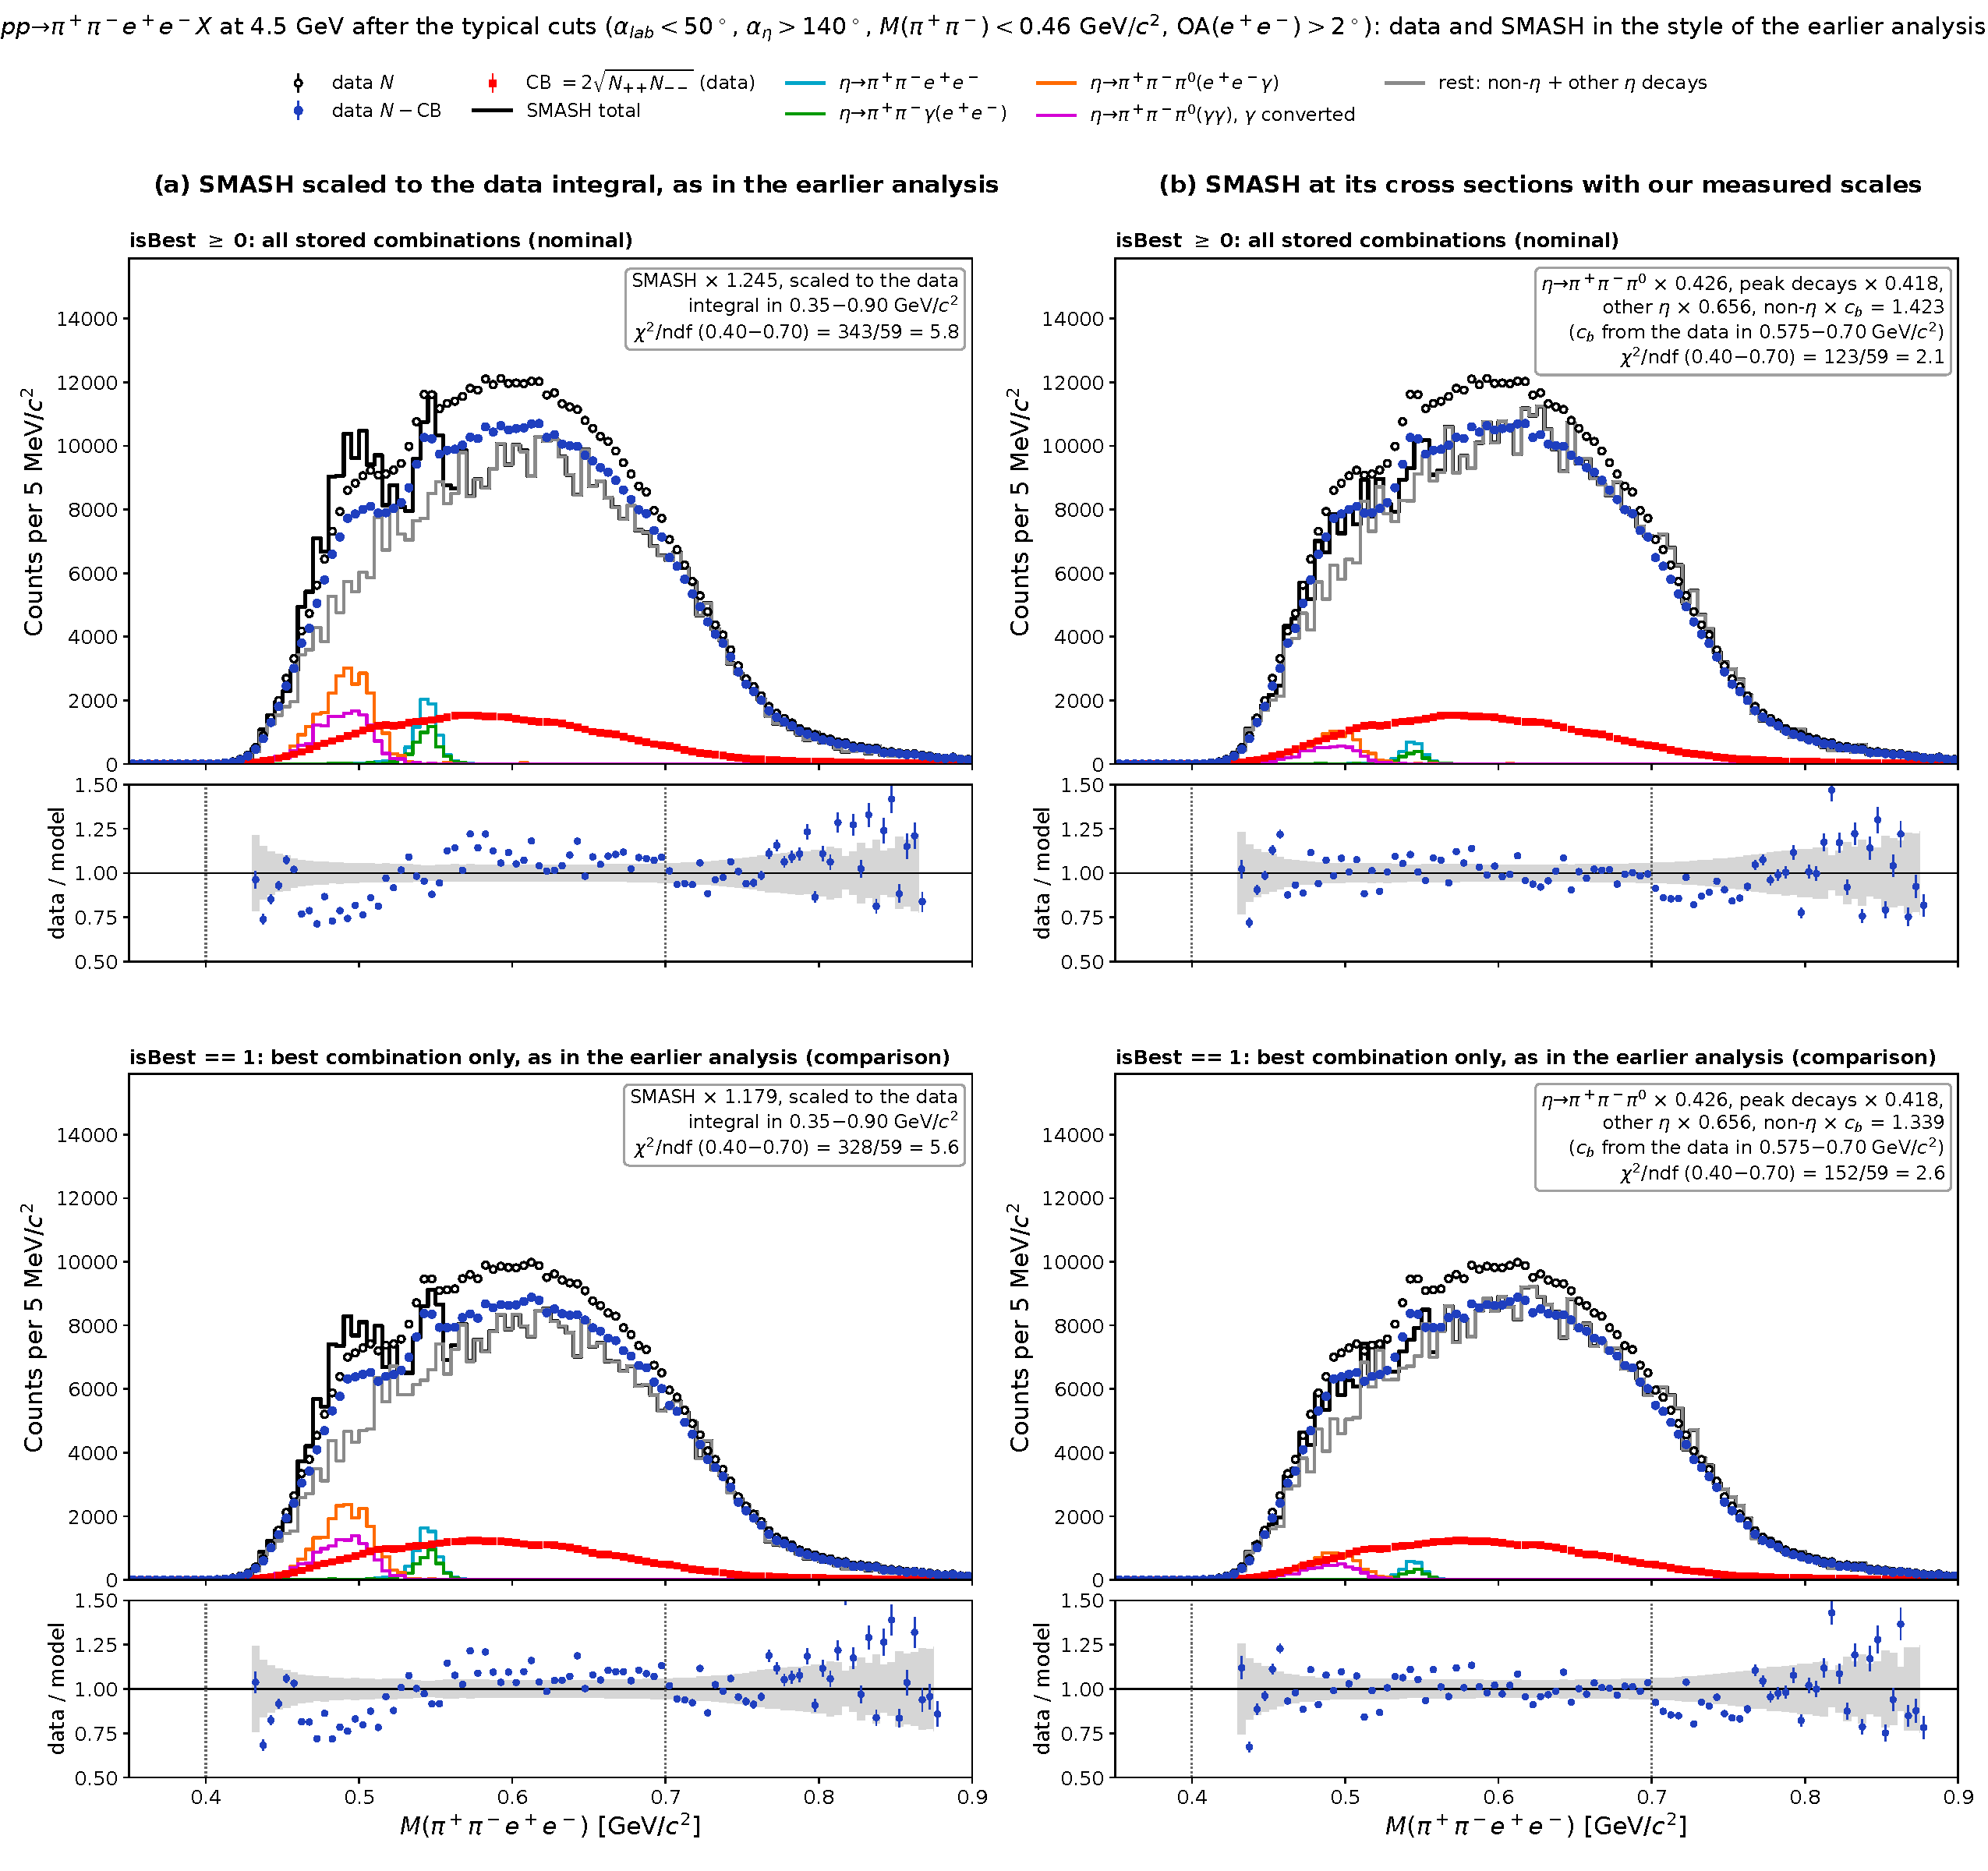
\includegraphics[width=0.86\textwidth]{figs_all/prevstyle_m4_E1.pdf}
\caption{\textbf{What it shows: after the typical cuts, SMASH scaled to the data integral (as in the earlier analysis) gets the total right
but the parts wrong. It is about 20\,\% too high in the bump and 10\,\% too low above the peak. With our measured scales SMASH describes the data
up to 0.70\,\GeVcc ($\chi^2/\mathrm{ndf}$ 2.1 instead of 5.8).}
Selection: \ptthreecap{}; event vertex in the target region ($\vz>-160$\,mm); particles identified by their START-free velocity \betanew (pions
within $3\sigma$, leptons within $5\sigma$ of their band; leptons with a RICH ring, pions without); energy-loss-corrected momenta of all four tracks;
angle between the \pipi and \ee systems below $50^\circ$ in the laboratory and above $140^\circ$ in the $\eta$ rest frame; \Mpipi$<0.46$\,\GeVcc;
\ee opening angle above $2^\circ$; all \Mee. Top row: all stored combinations of each event (isBest $\ge0$, the nominal choice; an event can give
more than one count). Bottom row: the best combination only (isBest $=1$, in the data and in SMASH), shown only to reproduce the earlier analysis.
Open black circles: data counts $N$; red squares: CB $=2\sqrt{N_{++}N_{--}}$ from the like-sign data with the same cuts; blue points:
$N-\mathrm{CB}$; counts per 5\,\MeVcc, $L=6079.2\,\nbinv$. Lines: SMASH p+p at 4.5\,GeV (standard, lepton and $\eta$ sets) in expected counts,
cross sections $\times$ PDG branching ratios $\times$ the $\eta$-decay weights, masses moved to the data scale ($\Mfour\times0.99615$,
$\Mpipi\times0.9952$), the Dalitz pairs of $\eta\to\pipi\piz$ with per-count QED weights for the $\gamma^*$ decay angle. Black: SMASH total;
cyan: $\eta\to\ppee$; green: $\eta\to\pipi\gamma$ with the photon converted; orange: $\eta\to\pipi\piz$, $\piz\to\ee\gamma$; magenta:
$\eta\to\pipi\piz$, $\piz\to\gamma\gamma$ with one photon converted; grey: the rest (non-$\eta$ pairs and other $\eta$ decays). (a) Every SMASH
line $\times$ one factor that matches the integral of $N-\mathrm{CB}$ in 0.35--0.90\,\GeVcc (1.245 and 1.179). (b) $\eta\to\pipi\piz\times0.426$,
the two peak decays $\times0.418$, other $\eta$ decays $\times0.656$, non-$\eta$ background $\times c_b$ (1.423 and 1.339, fitted to the data in
0.575--0.70\,\GeVcc). Lower pads: data $(N-\mathrm{CB})$/model; grey band: SMASH statistics; dotted lines: the $\chi^2$ range 0.40--0.70\,\GeVcc
($\chi^2$ with data and SMASH errors). Not to over-read: scaling to the integral hides the separate $\eta$ and background levels, so (a) says
nothing about the $\eta$ yields. The CB always comes from the data; the simulation never provides it. For isBest $=1$ the like-sign formula is the
naive one of the earlier analysis (caveats below). Numbers: Table~\ref{tab:e1prev}.}
\label{fig:e1-prev-m4}
\end{figure}

\begin{figure}[p]
\centering
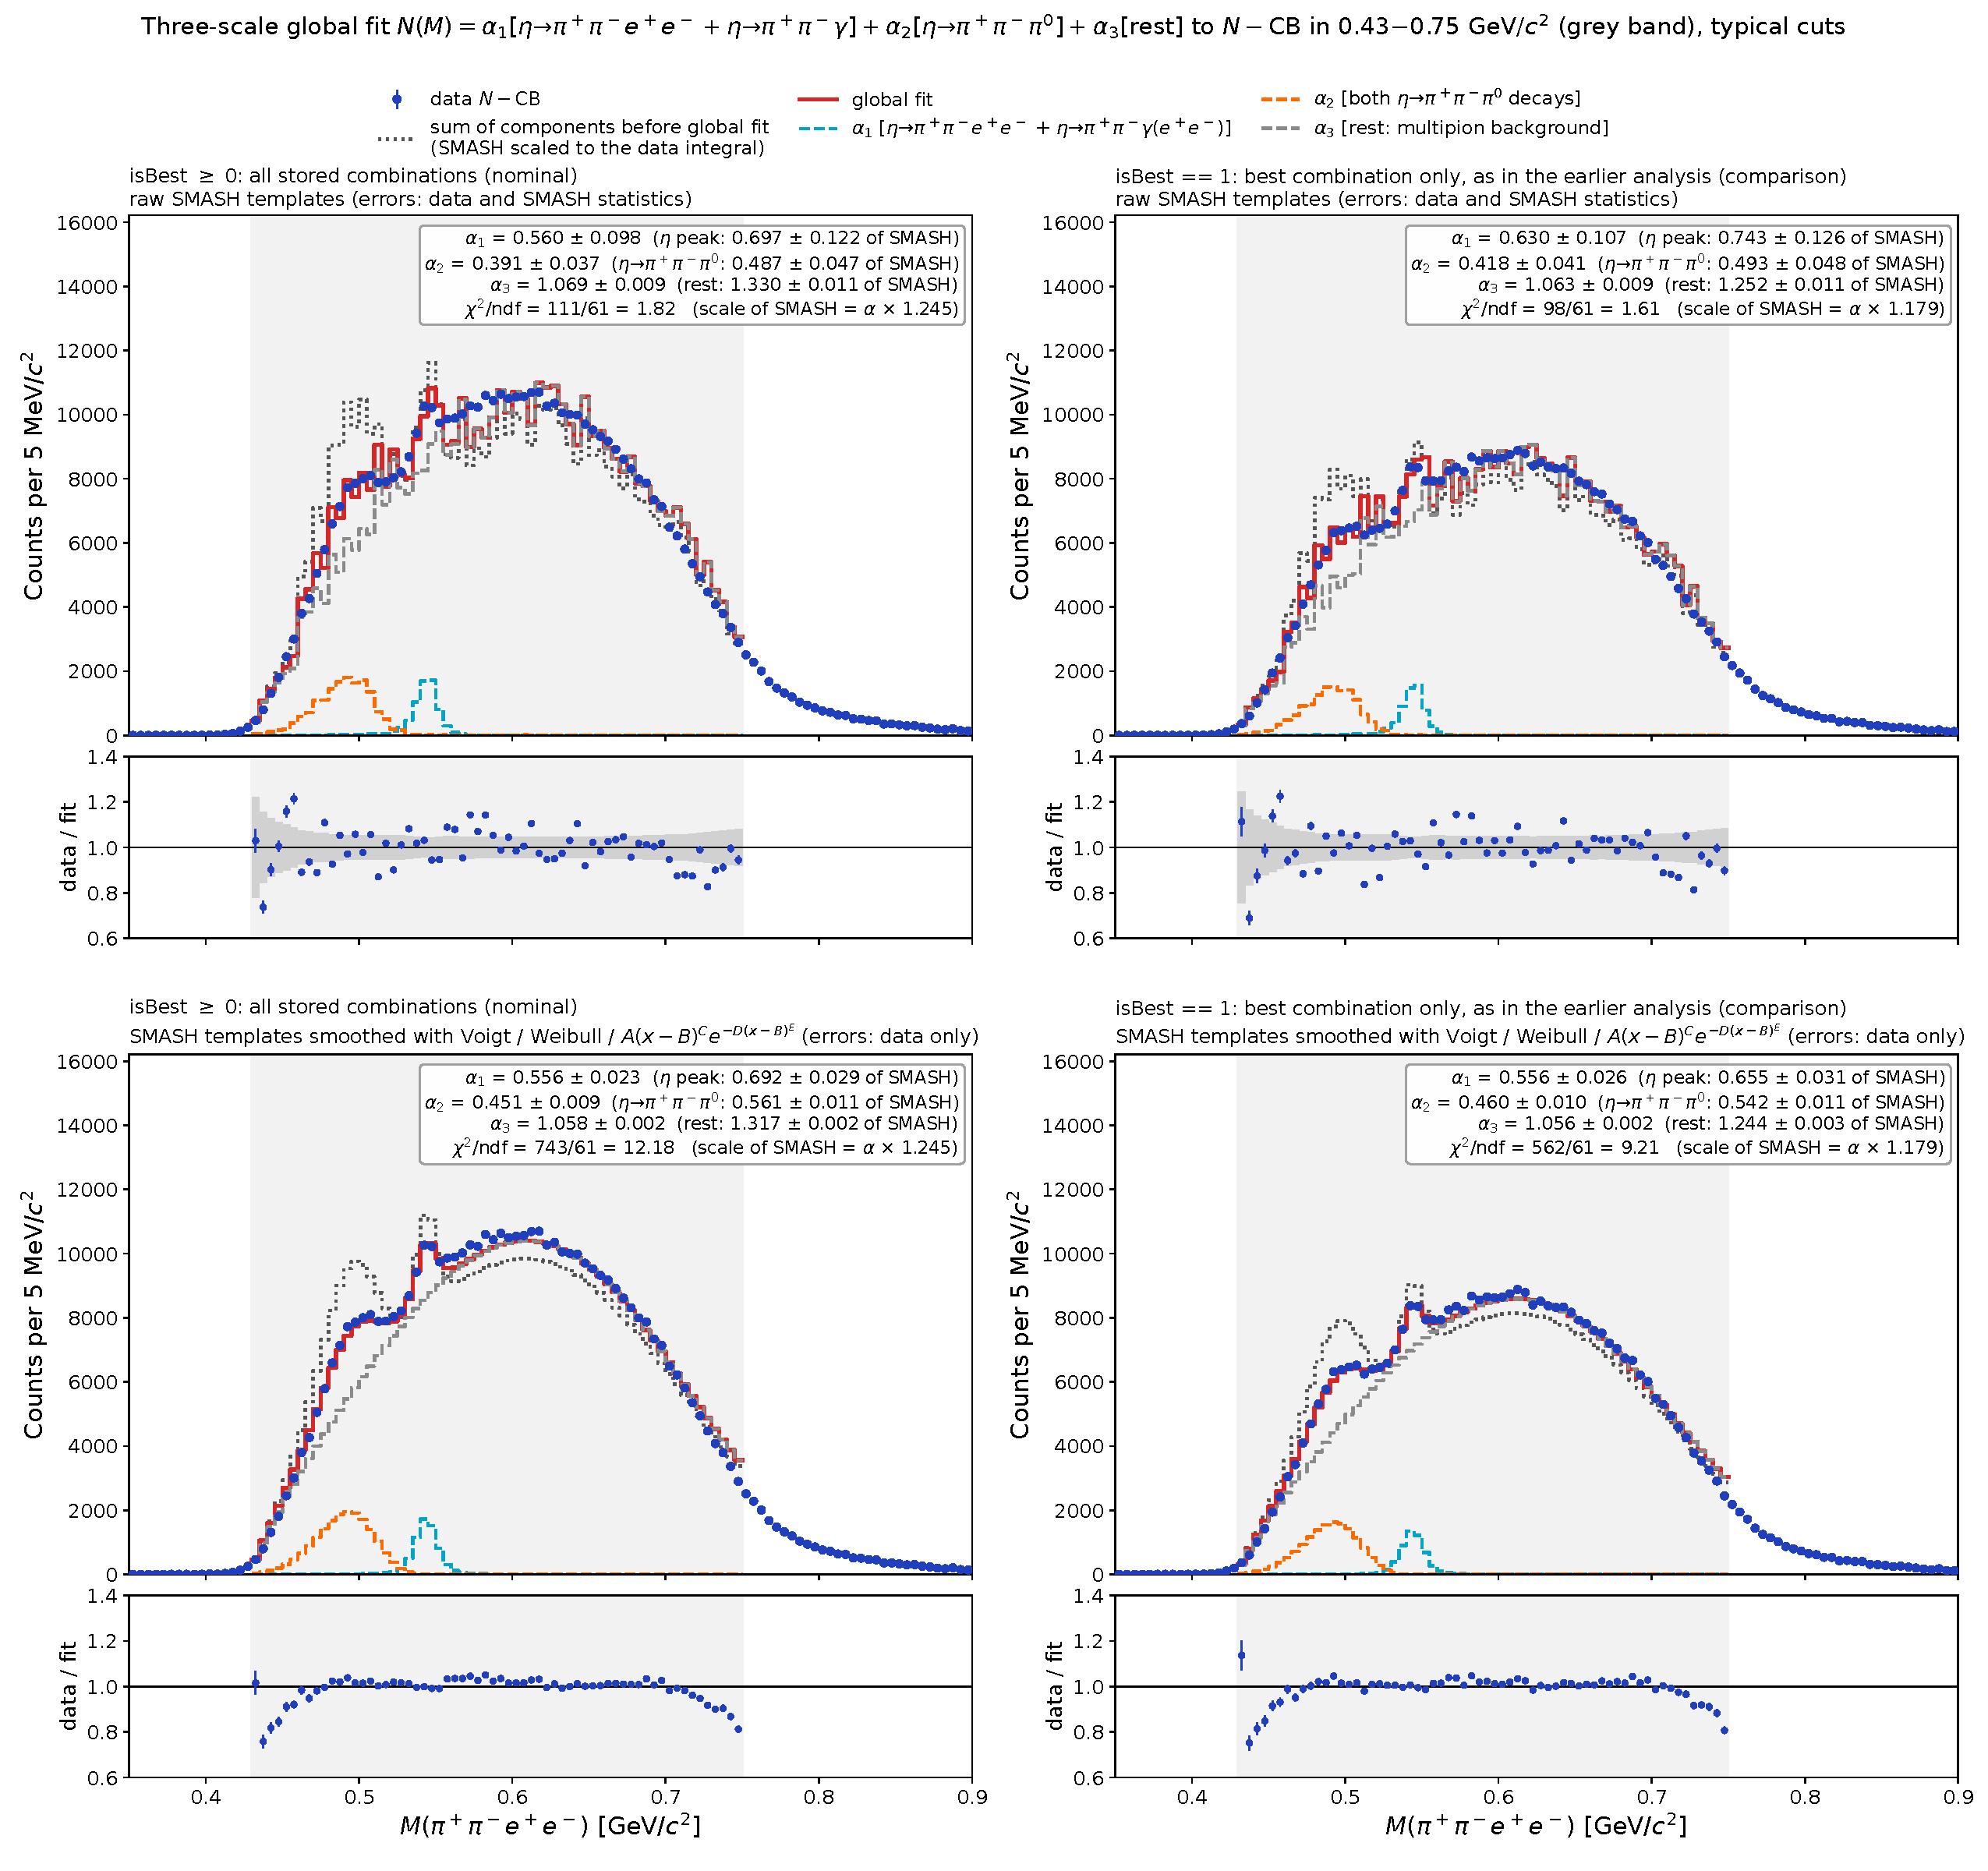
\includegraphics[width=0.95\textwidth]{figs_all/prevstyle_globalfit_E1.pdf}
\caption{\textbf{What it shows: the three-scale global fit of the earlier analysis describes the spectrum, but its $\eta$ scales depend on how
the SMASH templates are treated. The $\eta$ peak comes out at 0.69--0.70 of SMASH and the $\eta\to\pipi\piz$ decays at 0.49--0.56, against
0.418 and 0.426 from our dedicated measurements.}
Selection: as in Fig.~\ref{fig:e1-prev-m4}: \ptthreecap{}, event vertex at $\vz>-160$\,mm, \betanew identification, corrected momenta, angle
between the \pipi and \ee systems below $50^\circ$ in the laboratory and above $140^\circ$ in the $\eta$ rest frame, \Mpipi$<0.46$\,\GeVcc, \ee
opening angle above $2^\circ$; CB from the like-sign data with the same cuts. Fit of $N-\mathrm{CB}$ in 0.43--0.75\,\GeVcc (grey band,
5\,\MeVcc bins) with $\alpha_1\,[\eta\to\ppee+\eta\to\pipi\gamma$ (converted)$]+\alpha_2\,[$both $\eta\to\pipi\piz$ decays$]+\alpha_3\,[$all
other SMASH pairs, ``multipion background''$]$. Before the fit every component is SMASH scaled to the data integral (dotted: their sum). Red: the
global fit; dashed: the three components after the fit; blue: data $N-\mathrm{CB}$. The box gives the $\alpha$s and, multiplied by the integral
factor, the scales relative to SMASH, and $\chi^2/\mathrm{ndf}$. Top: raw SMASH templates, errors of the data and of the SMASH statistics.
Bottom: SMASH templates smoothed with a Voigt function ($\eta$ peak), a Weibull function ($\eta\to\pipi\piz$) and $A(x-B)^C\exp[-D(x-B)^E]$
(rest, fitted in 0.43--0.75\,\GeVcc), errors of the data only. Left: all stored combinations (isBest $\ge0$, nominal). Right: best combination
only (isBest $=1$, as in the earlier analysis, comparison). Lower pads: data/fit. Not to over-read: the multipion background is 95\,\% of the
counts in the fit range. Its SMASH shape is wrong at the level of the data errors ($\chi^2/\mathrm{ndf}$ 9--12 even with smooth templates), and
the small $\eta$ components (1.4\,\% and 3.5\,\% of the counts) absorb this. With the rest smoothed over 0.40--0.90\,\GeVcc instead, the peak scale
drops to 0.48 and the bump scale rises to 0.70. The $\alpha$s are a display, not yields.}
\label{fig:e1-prev-gfit}
\end{figure}

\begin{figure}[tbp]
\centering
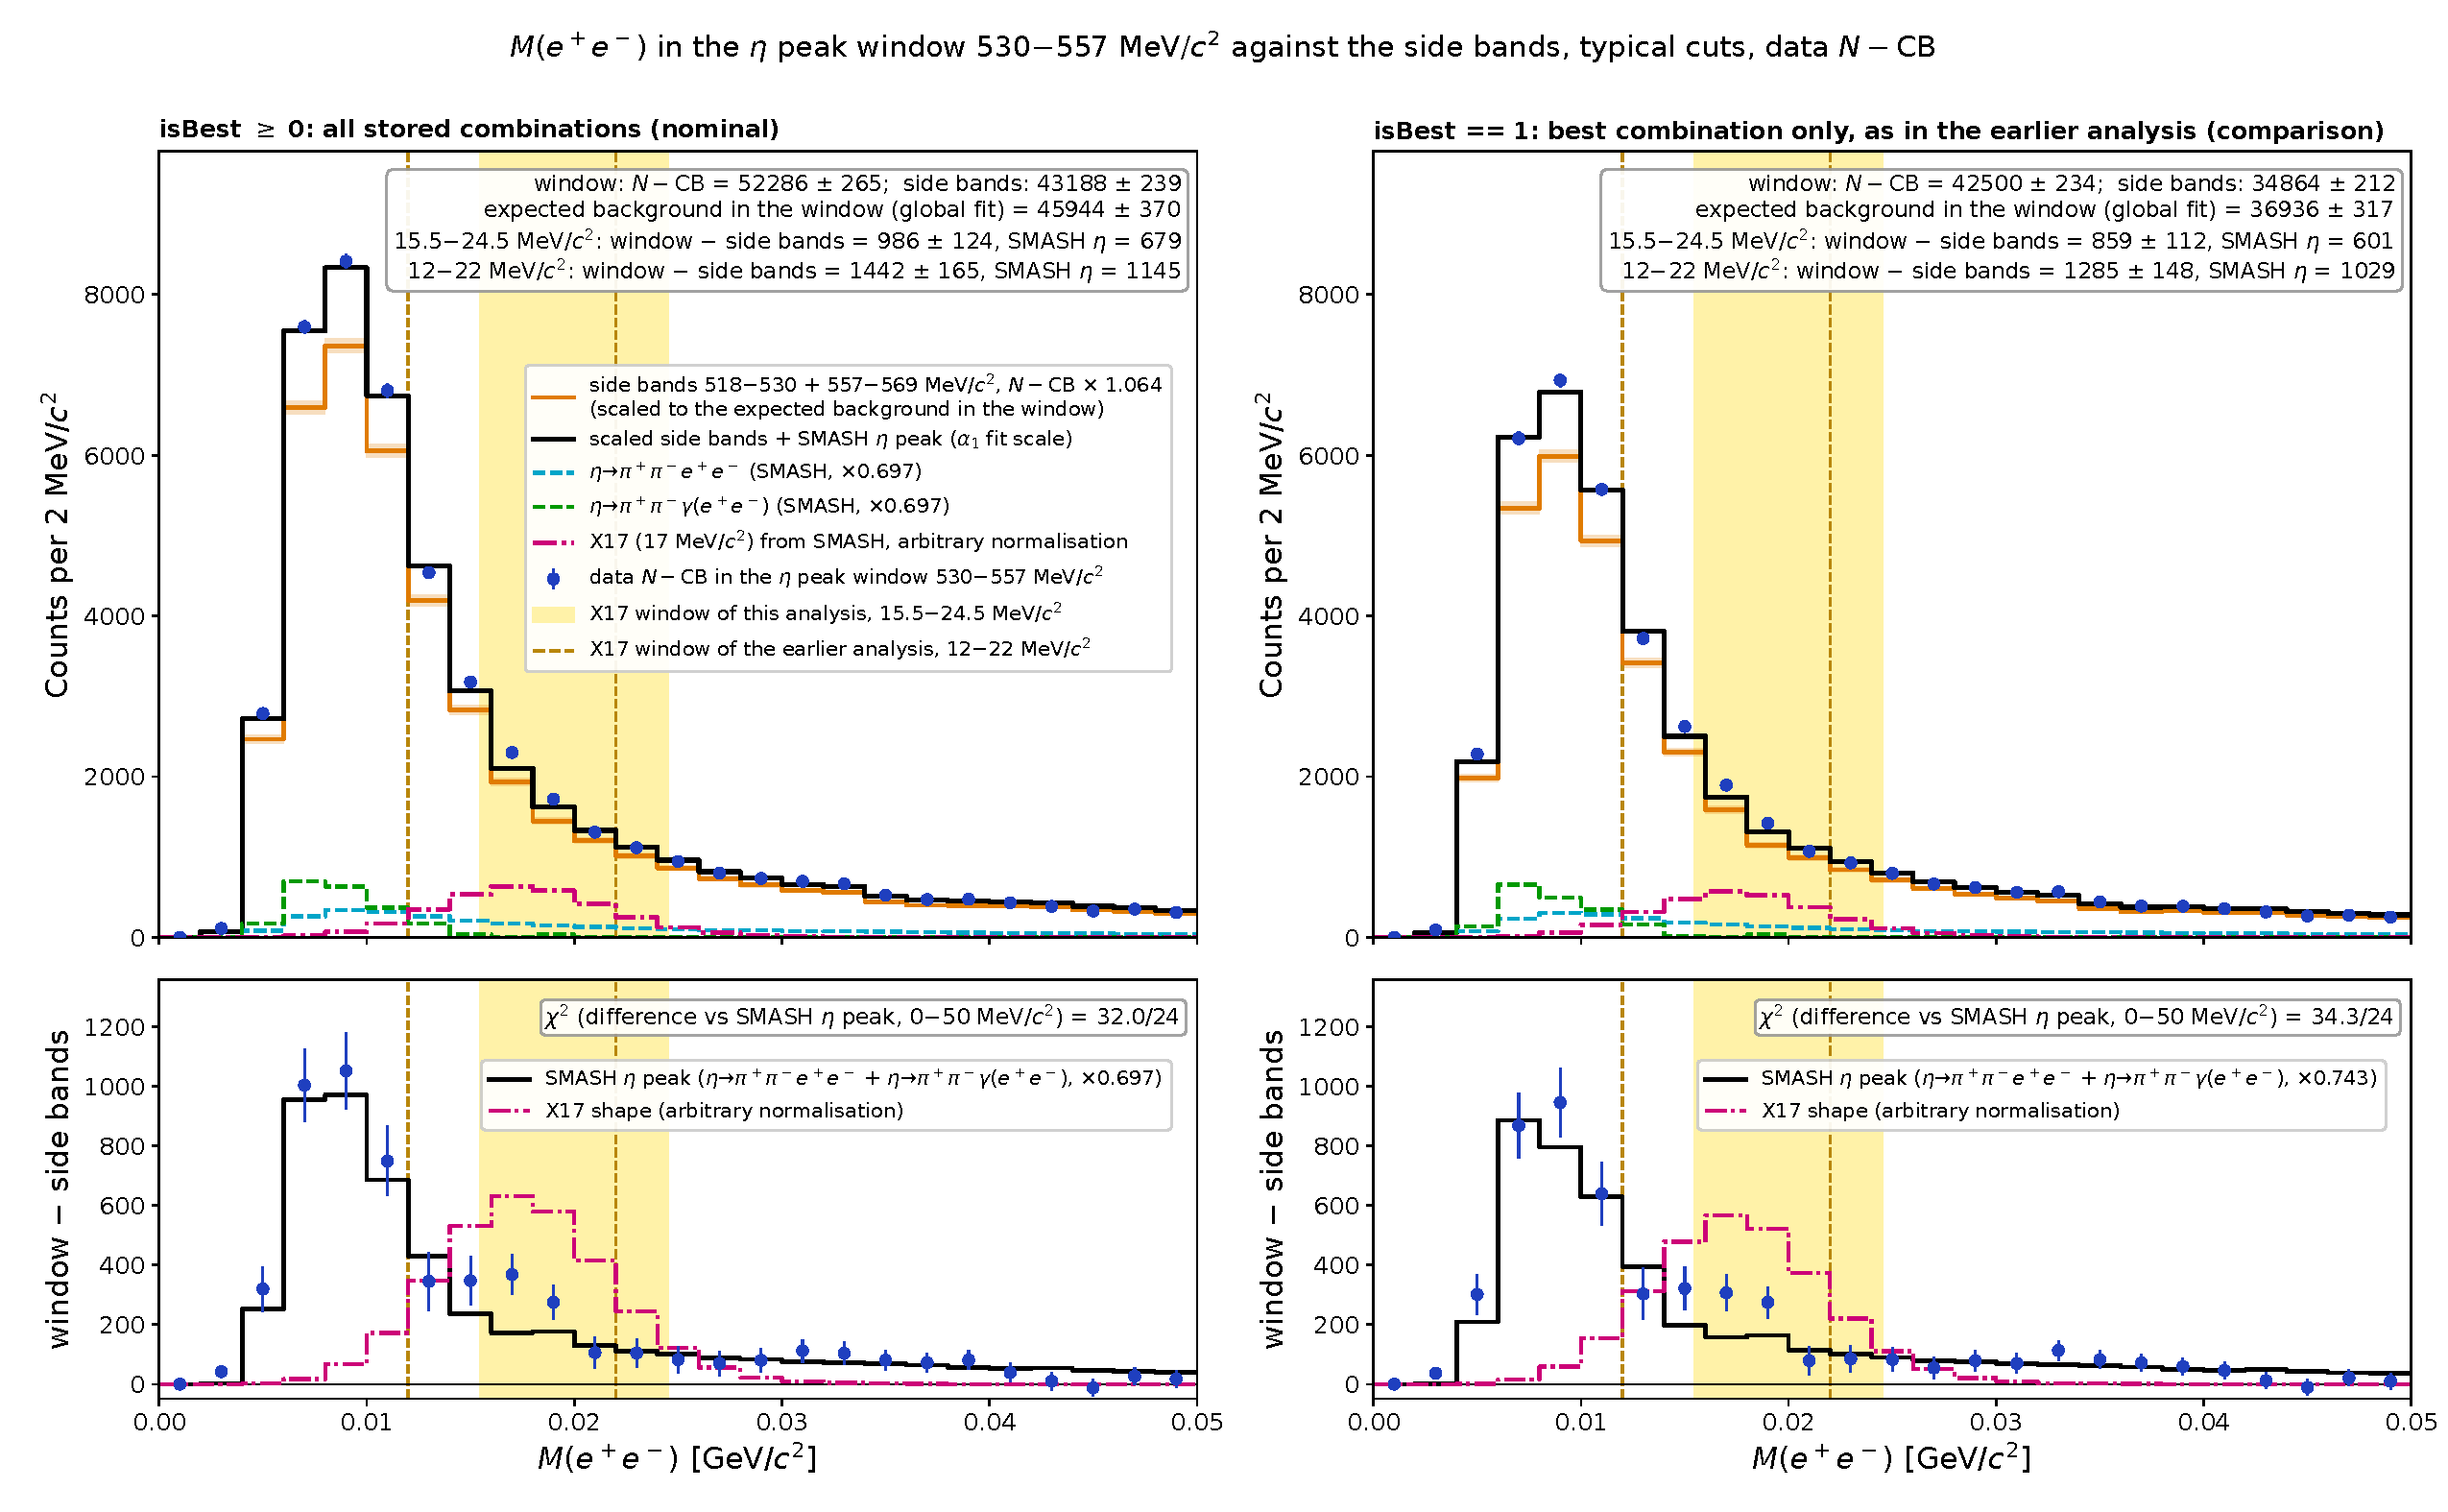
\includegraphics[width=0.95\textwidth]{figs_all/prevstyle_mee_E1.pdf}
\caption{\textbf{What it shows: in the $\eta$ peak window the \ee mass spectrum minus the scaled side bands follows the shape SMASH predicts
for the $\eta$ decays. In the X17 windows the small residual ($307\pm124$ counts in 15.5--24.5\,\MeVcc) changes sign when the side-band
normalisation or the $\eta$ scale is changed within reason, so this view cannot test an X17 signal.}
Selection: as in Fig.~\ref{fig:e1-prev-m4} (\ptthreecap{}, event vertex at $\vz>-160$\,mm, \betanew identification, corrected momenta, angle
between the \pipi and \ee systems below $50^\circ$ in the laboratory and above $140^\circ$ in the $\eta$ rest frame, \Mpipi$<0.46$\,\GeVcc, \ee
opening angle above $2^\circ$), with \Mfour in the $\eta$ peak window 530--557\,\MeVcc or in the side bands 518--530 and 557--569\,\MeVcc.
Blue points: data $N-\mathrm{CB}$ in the window, counts per 2\,\MeVcc; CB from the like-sign data with the same cuts. Orange: $N-\mathrm{CB}$ of
the side bands, scaled by $k$ to the background expected in the window from the global fit (raw templates; $k=1.064$ and 1.060); band: its
statistical error. Black: scaled side bands + the SMASH $\eta$ peak ($\eta\to\ppee$ + $\eta\to\pipi\gamma$ with the photon converted, $\times$ the
global-fit scale 0.697 and 0.743); dashed: the two decays alone; dash-dotted magenta: X17 (17\,\MeVcc) from SMASH, arbitrary normalisation
(about ten times an X17 at the present limit). Yellow band: X17 window of this analysis, 15.5--24.5\,\MeVcc; dashed brown lines: the earlier
analysis' window, 12--22\,\MeVcc. Lower pads: window $-$ scaled side bands, against the SMASH $\eta$ peak. Left: all stored combinations (isBest
$\ge0$, nominal); right: best combination only (isBest $=1$, as in the earlier analysis, comparison). Not to over-read: the side-band factor is not
measured. The plain width ratio (27/24) instead of the fit value turns the residual into $-62$ counts, and our peak scale 0.418 instead of the
fit's 0.697 turns it into $+579$. The side bands also contain about 700 counts of the $\eta$ peak tails. The X17 search uses the frozen side-band
likelihood of \S\ref{sec:x17}, not this view.}
\label{fig:e1-prev-mee}
\end{figure}

\begin{table}[tbp]
\centering
\caption{\textbf{What it shows: integral scaling matches the total but misses the bump and the region above the peak; the $\eta$ scales of the
global fit move with the template treatment; the side-band residual in the X17 window changes sign with reasonable choices.}
Selection: as in Fig.~\ref{fig:e1-prev-m4} (\ptthreecap{}, $\vz>-160$\,mm, \betanew identification, corrected momenta, the typical cuts
\cs{E1}); CB from the like-sign data with the same cuts. isBest $=1$ only reproduces the earlier approach. (a) SMASH scaled to the data
integral and with our measured scales; $\chi^2$ in 0.40--0.70\,\GeVcc (60 bins, errors of the data and of the SMASH statistics); regions in \GeVcc.
(b) Three-scale global fit in 0.43--0.75\,\GeVcc (64 bins): $\alpha_1$ the $\eta$ peak, $\alpha_2$ the $\eta\to\pipi\piz$ decays, $\alpha_3$
the rest; $\alpha s$: the scale relative to SMASH (relative errors as for $\alpha$); ``raw'': errors of the data and the SMASH statistics unless
stated. (c) \Mee in the $\eta$ window (\Mfour 530--557\,\MeVcc) minus the side bands (518--530 + 557--569\,\MeVcc) scaled by $k$; residual $=$ difference $-$ SMASH $\eta$ peak, errors:
statistics, side-band normalisation, SMASH statistics. (d), the demonstration with the background fixed on the slope, follows in the
continuation of this table. The common 6.9\,\% of $L$ is not included. Source: \code{prevstyle_results.md}.}
\label{tab:e1prev}
\footnotesize
\setlength{\tabcolsep}{4pt}\renewcommand{\arraystretch}{1.05}
\begin{tabular}{@{}l r r r r@{}}
\toprule
(a) & \multicolumn{2}{c}{isBest $\ge0$ (nominal)} & \multicolumn{2}{c}{isBest $=1$ (comparison)} \\
\cmidrule(lr){2-3}\cmidrule(lr){4-5}
 & integral scaling & measured scales & integral scaling & measured scales \\
\midrule
factor ($s$ or $c_b$) & $s=1.2445\pm0.0088$ & $c_b=1.423\pm0.015$ & $s=1.1785\pm0.0084$ & $c_b=1.339\pm0.015$ \\
$\chi^2/\mathrm{ndf}$, 0.40--0.70 & $343/59=5.8$ & $123/59=2.1$ & $328/59=5.6$ & $152/59=2.6$ \\
data/model 0.35--0.455 & 0.949 & 0.992 & 0.934 & 0.980 \\
\quad bump window 0.455--0.5225 & 0.814 & 0.996 & 0.818 & 0.993 \\
\quad peak window 0.5336--0.5542 & 0.951 & 1.045 & 0.960 & 1.051 \\
\quad 0.56--0.70 & 1.088 & 1.004 & 1.082 & 1.003 \\
\quad 0.70--0.90 & 0.997 & 0.911 & 0.997 & 0.913 \\
\bottomrule
\end{tabular}

\vspace{0.6em}
\setlength{\tabcolsep}{3.5pt}
\begin{tabularx}{\textwidth}{@{}L r r r r r r r@{}}
\toprule
(b) template treatment & $\alpha_1$ & $\alpha_2$ & $\alpha_3$ & $\alpha_1 s$ & $\alpha_2 s$ & $\alpha_3 s$ & $\chi^2/\mathrm{ndf}$ \\
\midrule
\multicolumn{8}{@{}l}{isBest $\ge0$ (nominal), $s=1.2445$} \\
raw & $0.560\pm0.098$ & $0.391\pm0.037$ & $1.069\pm0.009$ & 0.697 & 0.487 & 1.330 & $111/61=1.8$ \\
raw, data errors only & $0.579\pm0.023$ & $0.384\pm0.009$ & $1.060\pm0.002$ & 0.720 & 0.478 & 1.319 & $2202/61=36$ \\
smoothed (nominal) & $0.556\pm0.023$ & $0.451\pm0.009$ & $1.058\pm0.002$ & 0.692 & 0.561 & 1.317 & $743/61=12.2$ \\
smoothed, rest on 0.40--0.90 & $0.384\pm0.024$ & $0.566\pm0.009$ & $1.065\pm0.002$ & 0.478 & 0.704 & 1.325 & $1111/61=18.2$ \\
\midrule
\multicolumn{8}{@{}l}{isBest $=1$ (comparison), $s=1.1785$} \\
raw & $0.630\pm0.107$ & $0.418\pm0.041$ & $1.063\pm0.009$ & 0.743 & 0.493 & 1.252 & $98.5/61=1.6$ \\
raw, data errors only & $0.646\pm0.026$ & $0.409\pm0.009$ & $1.054\pm0.002$ & 0.762 & 0.482 & 1.242 & $1905/61=31$ \\
smoothed (nominal) & $0.556\pm0.027$ & $0.460\pm0.010$ & $1.056\pm0.002$ & 0.655 & 0.542 & 1.244 & $562/61=9.2$ \\
smoothed, rest on 0.40--0.90 & $0.386\pm0.027$ & $0.580\pm0.009$ & $1.062\pm0.002$ & 0.454 & 0.684 & 1.251 & $1041/61=17.1$ \\
\bottomrule
\end{tabularx}

\vspace{0.6em}
\setlength{\tabcolsep}{4pt}
\begin{tabularx}{\textwidth}{@{}L r r@{}}
\toprule
(c) \Mee in the $\eta$ window minus the scaled side bands & isBest $\ge0$ (nominal) & isBest $=1$ (comparison) \\
\midrule
side-band factor $k$: global fit / smoothed fit / width ratio 27/24 & $1.064\pm0.010$ / 1.075 / 1.125 & $1.060\pm0.011$ / 1.087 / 1.125 \\
all \Mee (0--50\,\MeVcc): difference; SMASH $\eta$ peak; $\chi^2$ of the shape & $5476\pm312$; 4964; 32.0/24 & $4854\pm280$; 4412; 34.3/24 \\
15.5--24.5\,\MeVcc (this analysis): difference; SMASH $\eta$ peak & $986\pm124$; 679 & $859\pm112$; 601 \\
\quad residual & $307\pm124\pm63\pm26$ & $258\pm112\pm55\pm20$ \\
\quad residual with $k=27/24$ / smoothed $k$ / peak at $\aP=0.418$ & $-62$ / 239 / 579 & $-67$ / 123 / 520 \\
12--22\,\MeVcc (earlier analysis): difference; SMASH $\eta$ peak & $1442\pm165$; 1145 & $1285\pm148$; 1029 \\
\quad residual & $296\pm165\pm113\pm63$ & $256\pm148\pm99\pm60$ \\
\quad residual with $k=27/24$ / smoothed $k$ / peak at $\aP=0.418$ & $-371$ / 174 / 755 & $-328$ / 14 / 706 \\
\bottomrule
\end{tabularx}
\end{table}

\textbf{Results in plain words.}
\begin{enumerate}\setlength{\itemsep}{1pt}
\item \textbf{Scaling SMASH to the data integral hides the separate $\eta$ and background levels.} One factor for everything ($\times1.245$ for
      isBest $\ge0$) makes the total right by construction, but the parts stay wrong: SMASH is about 20\,\% too high in the bump window
      (data/model 0.81) and about 10\,\% too low just above the peak (1.09 in 0.56--0.70\,\GeVcc); $\chi^2/\mathrm{ndf}=343/59=5.8$ in
      0.40--0.70\,\GeVcc. Integral scaling cannot say how large the $\eta$ signals are.
\item \textbf{With our measured scales SMASH describes the data up to 0.70\,\GeVcc.} With the $\eta$ at about 0.42 of SMASH and the non-$\eta$
      background $\times1.42$, data/model is 0.996 in the bump window, 1.045 in the peak window and 1.004 in 0.56--0.70\,\GeVcc;
      $\chi^2/\mathrm{ndf}=123/59=2.1$. Above 0.70\,\GeVcc the model is 9\,\% too high (0.91), as in Fig.~\ref{fig:e1-m4E1}. SMASH as it is,
      or with one common factor, does not give this picture.
\item \textbf{The global fit is a display, not a measurement of the $\eta$ yields.} Leaving out the raw fits with data errors only, which ignore the
      template statistics, four of the six fits give 0.65--0.74 of SMASH for the peak, and the two with the rest smoothed over 0.40--0.90\,\GeVcc
      give 0.45--0.48; the bump comes out at 0.49--0.70. The spread between
      the template treatments (0.14--0.22) is 7--20 times the statistical error of the smoothed fits. The cause: the multipion background is 95\,\% of
      the counts in 0.43--0.75\,\GeVcc (88--89\,\% in the $\eta$ peak window), its SMASH shape is not right at the level of the data errors (about
      1.2\,\% per 5\,\MeVcc bin; data/fit 0.75--0.9 at 0.43--0.46 and 0.8--0.9 at 0.72--0.75\,\GeVcc), and the two small $\eta$ templates (1.4\,\%
      and 3.3--3.8\,\% of the counts) absorb this shape error: a 1\,\% change of the background under the peak moves the peak scale by about 0.05.
      With raw templates the SMASH statistics hide the problem: the $\eta$ peak template rests on about 940 effective simulated counts, its conversion
      part on 127, so one simulated count stands for 10--28 expected counts; with data errors only, the raw fit has $\chi^2/\mathrm{ndf}=36$, of
      which about two thirds is template noise.
\item \textbf{Against our measurements.} Our robust values are $\aP=0.418$ (peak, side-band estimator), $\feta=0.426$ (bump, from the distance to
      its kinematic edge, which does not need the background level) and $0.46\pm0.06$ (common $\eta$ scale of the flexible description,
      \S\ref{sec:flex}). The global fit gives a larger peak and a larger bump. The two approaches agree in one sense only: SMASH's $\eta$ must come
      down by a factor of about 1.4--2.4, and its non-$\eta$ background must go up by 25--45\,\% (rest $\times$1.24--1.33 in the global fit,
      $c_b=1.34$--1.45 with our scales; they differ because the rest also holds the other $\eta$ decays and $c_b$ is set in 0.575--0.70\,\GeVcc
      only). The earlier style cannot replace the edge and peak measurements; its $\eta$ numbers move with choices that our methods do not have.
\item \textbf{The \Mee side-band view cannot test X17.} The $\eta$ window minus the scaled side bands follows the SMASH $\eta$ peak shape
      ($\chi^2=32.0/24$). In the X17 window 15.5--24.5\,\MeVcc the difference is $986\pm124$ counts against 679 of the SMASH $\eta$ peak, a residual
      of $307\pm124\,(\mathrm{stat})\pm63$ (side-band normalisation) counts. It is not a signal: with the plain width ratio 27/24 as the side-band
      factor it becomes $-62$, with our peak scale 0.418 instead of the fit's 0.697 it becomes $+579$. The window 12--22\,\MeVcc of the earlier
      analysis behaves the same way ($296\pm165$; $-371$; $+755$). The frozen side-band likelihood of \S\ref{sec:x17} remains the reference.
\item \textbf{isBest $=1$ gives the same picture.} In the data the best combination keeps 0.825 of $N-\mathrm{CB}$ in 0.35--0.90\,\GeVcc; in
      SMASH it keeps 0.871, so the simulated choice keeps 5--6\,\% more than the data's. This lowers the integral factor to 1.179 and $c_b$ to
      1.339; the scaled model fits slightly worse ($\chi^2/\mathrm{ndf}=2.6$). The CB share is the same: CB$/N$ 0.105 against 0.107.
\end{enumerate}

\textbf{Caveats of this view.} (1) For isBest $=1$ the CB is the naive like-sign formula of the best combinations, as in the earlier analysis; in
the \ee study this formula overestimated the CB of best pairs (a like-sign combination without a competitor is always flagged best). It is not
corrected here, so the isBest $=1$ numbers reproduce the earlier approach and are not a result. (2) The simulated best-combination choice follows the
PAT time $\chi^2$ with resolutions that do not match the data, so it is not realistic; this is why $s$ and $c_b$ differ between the two choices.
(3) $c_b=1.423$ uses our separate $\eta$ scales; with every $\eta$ channel $\times0.40$ (the rule of Fig.~\ref{fig:e1-m4E1}) it is 1.450, with the
same $\chi^2$ (123.1 against 123.2). (4) The 6.9\,\% of $L$ is common and not in the errors; the live time ($+7.3/-0$\,\%) is not applied.
\textbf{Checks.} With isBest $\ge0$ the package reproduces the comparison of Fig.~\ref{fig:e1-m4E1} exactly (data $N$, CB and its replica errors,
the like-sign counts in every 5\,\MeVcc bin, the X17 cell; every SMASH class to $10^{-9}$); independent counts on the ntuple and an independent
recomputation reproduce $s$, both $\chi^2$, $c_b$ and the raw global-fit $\alpha$s to all printed digits (39 automatic checks pass).

\begin{table}[!tbp]
\ContinuedFloat
\centering
\caption{(continued) \textbf{What it shows: with the background fixed on the slope, the two free $\eta$ scales hardly move with the fit range,
but they move with the normalisation window and with the background shape.} Selection: as in Fig.~\ref{fig:e1-prev-m4} (\ptthreecap{},
$\vz>-160$\,mm, \betanew identification, corrected momenta, the typical cuts \cs{E1}); CB from the like-sign data with the same cuts. (d)
Demonstration in the style of the earlier analysis; it is not a measurement and no result of this report uses it
(Fig.~\ref{fig:e1-prev-twoscale}). Background (non-$\eta$ SMASH $\times c_b$ + other $\eta$ decays $\times0.656$) fixed in the normalisation
window (``window''; nominal 0.575--0.70\,\GeVcc), then two free scales relative to SMASH fitted to $N-\mathrm{CB}$ in the fit range (``fit'';
nominal 0.43--0.575\,\GeVcc; 5\,\MeVcc bins; errors of the data and of the SMASH statistics): bump (both $\eta\to\pipi\piz$ decays) and peak
($\eta\to\ppee$ + $\eta\to\pipi\gamma$, photon converted). $c_b$ after one iteration with the fitted scales. Errors: fit and $c_b$ in quadrature
(separately in the second row of each block); in the other rows about those of the nominal row. Tilt: non-$\eta$ background $\times[1\pm0.03\,(M-M_0)/0.1\,
\GeVcc]$, $M_0$ the window centre. Masses in \GeVcc. Source: \code{prevstyle_results.md}, section~9.}
\label{tab:e1prev-d}
\footnotesize
\setlength{\tabcolsep}{4pt}\renewcommand{\arraystretch}{1.05}
\begin{tabular}{@{}l r r r r@{}}
\toprule
(d) demonstration, not a measurement & $c_b$ & bump & peak & $\chi^2/\mathrm{ndf}$ \\
\midrule
\multicolumn{5}{@{}l}{isBest $\ge0$ (nominal)} \\
nominal: window 0.575--0.70, fit 0.43--0.575 & $1.423\pm0.015$ & $0.455\pm0.049$ & $0.652\pm0.127$ & 50.8/27 \\
\quad errors: fit; from $c_b$ & & $\pm0.044$; $\pm0.021$ & $\pm0.116$; $\pm0.050$ & \\
\quad data errors only (no SMASH statistics) & 1.423 & $0.427\pm0.010$ & $0.631\pm0.027$ & 1076/27 \\
window 0.575--0.65 & 1.427 & 0.449 & 0.637 & 50.6/27 \\
window 0.60--0.70 & 1.403 & 0.481 & 0.716 & 52.2/27 \\
window 0.575--0.75 & 1.391 & 0.498 & 0.755 & 53.5/27 \\
fit 0.40--0.575 & 1.423 & 0.461 & 0.651 & 87.6/33 \\
fit 0.45--0.575 & 1.423 & 0.458 & 0.651 & 47.2/23 \\
fit 0.47--0.575 & 1.423 & 0.460 & 0.651 & 37.1/19 \\
fit 0.43--0.56 & 1.423 & 0.455 & 0.648 & 42.0/24 \\
background shape tilted $+3$\,\% per 0.1\,\GeVcc & 1.424 & 0.541 & 0.780 & 52.9/27 \\
background shape tilted $-3$\,\% per 0.1\,\GeVcc & 1.421 & 0.369 & 0.525 & 52.0/27 \\
\midrule
\multicolumn{5}{@{}l}{isBest $=1$ (comparison)} \\
nominal: window 0.575--0.70, fit 0.43--0.575 & $1.339\pm0.015$ & $0.460\pm0.050$ & $0.689\pm0.131$ & 49.5/27 \\
\quad errors: fit; from $c_b$ & & $\pm0.046$; $\pm0.020$ & $\pm0.121$; $\pm0.050$ & \\
\quad data errors only (no SMASH statistics) & 1.339 & $0.430\pm0.010$ & $0.666\pm0.029$ & 1047/27 \\
window 0.575--0.65 & 1.337 & 0.462 & 0.696 & 49.5/27 \\
window 0.60--0.70 & 1.329 & 0.474 & 0.724 & 49.6/27 \\
window 0.575--0.75 & 1.311 & 0.498 & 0.783 & 50.2/27 \\
fit 0.40--0.575 & 1.339 & 0.460 & 0.690 & 123.8/33 \\
fit 0.45--0.575 & 1.339 & 0.464 & 0.689 & 44.9/23 \\
fit 0.47--0.575 & 1.339 & 0.456 & 0.689 & 38.7/19 \\
fit 0.43--0.56 & 1.339 & 0.460 & 0.688 & 44.1/24 \\
background shape tilted $+3$\,\% per 0.1\,\GeVcc & 1.340 & 0.541 & 0.812 & 49.3/27 \\
background shape tilted $-3$\,\% per 0.1\,\GeVcc & 1.338 & 0.380 & 0.568 & 52.4/27 \\
\bottomrule
\end{tabular}
\end{table}

\begin{figure}[tbp]
\centering
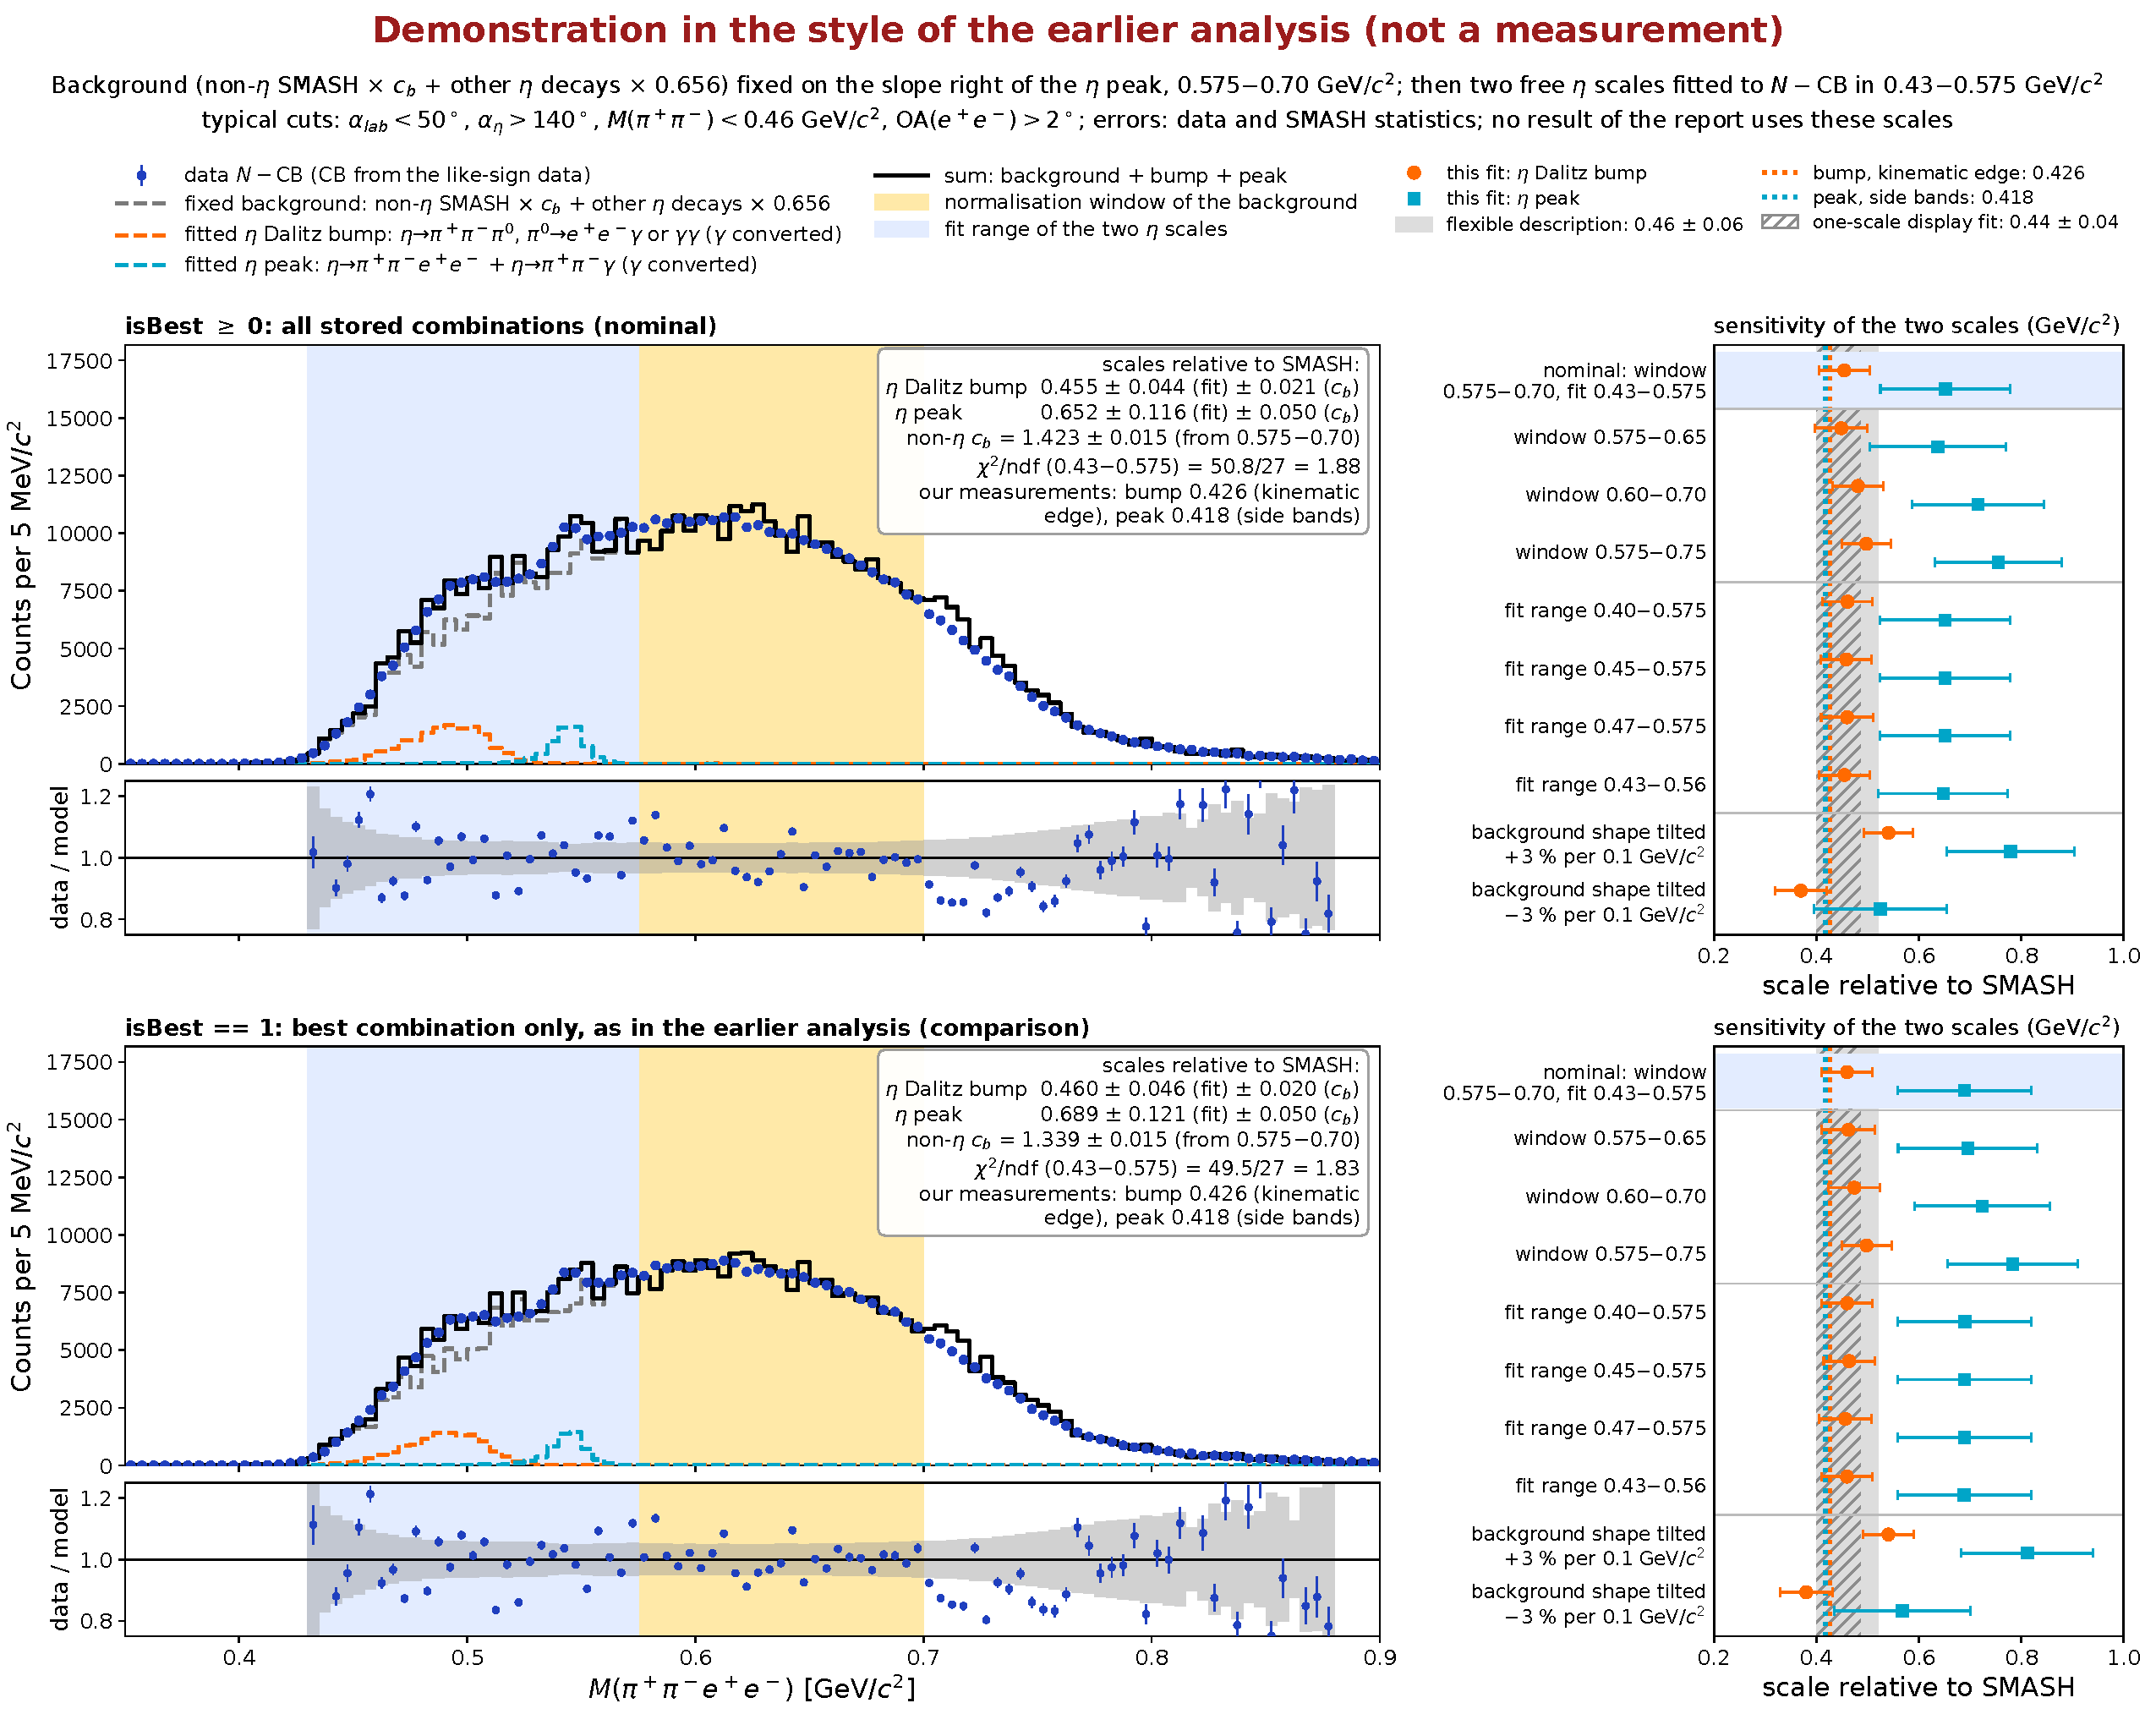
\includegraphics[width=0.90\textwidth]{figs_all/prevstyle_twoscale_E1.pdf}
\caption{\textbf{What it shows: with the background fixed on the slope right of the $\eta$ peak, two free scales put the $\eta$ Dalitz bump at
$0.455\pm0.049$ and the $\eta$ peak at $0.652\pm0.127$ of SMASH, but both move with the background shape that SMASH carries under them. This is a
demonstration in the style of the earlier analysis. It is not a measurement and no result of this report uses it.}
Selection: \ptthreecap{}; event vertex in the target region ($\vz>-160$\,mm); START-free velocity identification \betanew (pions within
$3\sigma$, leptons within $5\sigma$ of their band; leptons with a matched RICH ring, pions without); energy-loss-corrected momenta of all four
tracks; angle between the \pipi and \ee systems below $50^\circ$ in the laboratory and above $140^\circ$ in the $\eta$ rest frame;
\Mpipi$<0.46$\,\GeVcc; \ee opening angle above $2^\circ$; all \Mee. Top: all stored combinations of each event (isBest $\ge0$, nominal);
bottom: the best combination only (isBest $=1$, in the data and in SMASH; comparison). Left: data $N-\mathrm{CB}$ (blue; CB
$=2\sqrt{N_{++}N_{--}}$ from the like-sign data with the same cuts), counts per 5\,\MeVcc; SMASH in expected counts as in
Fig.~\ref{fig:e1-prev-m4}. Dashed grey: the fixed background, non-$\eta$ pairs $\times c_b$ (1.423 and 1.339, set in 0.575--0.70\,\GeVcc,
yellow) + other $\eta$ decays $\times0.656$. Dashed orange: $\eta\to\pipi\piz$ with $\piz\to\ee\gamma$ (QED-weighted) or $\piz\to\gamma\gamma$
with one photon converted; dashed cyan: $\eta\to\ppee$ + $\eta\to\pipi\gamma$ with the photon converted; each $\times$ its scale fitted in
0.43--0.575\,\GeVcc (light blue; errors of the data and of the SMASH statistics); black: the sum. Lower pads: data/model; grey band: SMASH
statistics. Right: the two scales (fit and $c_b$ errors in quadrature) for other normalisation windows, fit ranges and a background shape tilted
by $\pm3$\,\% per 0.1\,\GeVcc, against the bump from its kinematic edge, 0.426 (dotted orange), the peak from the side bands, 0.418 (dotted cyan),
the flexible description $0.46\pm0.06$ (grey) and the one-scale display fit after the typical cuts $0.44\pm0.04$ (hatched). Not to over-read: in
the bump window the fixed background is 5.4 times the bump and nothing measures it there; 1\,\% more background moves the bump scale by $-0.020$
and the peak scale by $-0.047$, and the tilts move the bump scale to 0.37--0.54 at almost the same $\chi^2$. The agreement of the bump scale with
0.426 is no test; the peak scale follows a few-per-cent shape mismatch of the background around the peak. The CB always comes from the data.
Numbers: Table~\ref{tab:e1prev}\,(d).}
\label{fig:e1-prev-twoscale}
\end{figure}

\textbf{Demonstration: the background fixed on the slope and two free $\eta$ scales} (package prevstyle, \code{prevstyle_twoscale.py};
Fig.~\ref{fig:e1-prev-twoscale}; Table~\ref{tab:e1prev}\,(d)).
\notebox{\textbf{This is a demonstration in the style of the earlier analysis. It is not a measurement and no result of this report uses it.}}
The analyst asked for the earlier style with the background fixed on the slope right of the $\eta$ peak and two separate free scales for the two
$\eta$ signals. (1) The non-$\eta$ SMASH background is multiplied by $c_b$ and the other $\eta$ decays by 0.656; $c_b$ makes the model match
$N-\mathrm{CB}$ in the normalisation window 0.575--0.70\,\GeVcc (start: bump $\times0.426$, peak $\times0.418$, which gives the $c_b$ of
display (b) exactly). (2) With this background fixed, one free scale for the $\eta$ Dalitz bump (both $\eta\to\pipi\piz$ decays: the \piz
Dalitz decay with its per-count QED weights, and $\piz\to\gamma\gamma$ with one photon converted) and one for the $\eta$ peak ($\eta\to\ppee$
and $\eta\to\pipi\gamma$ with the photon converted) are fitted to $N-\mathrm{CB}$ in 0.43--0.575\,\GeVcc (29 bins of 5\,\MeVcc; $\chi^2$ with
the errors of the data and of the SMASH statistics, iterated). (3) $c_b$ is recomputed once with the fitted scales and the fit is repeated.
The errors are those of the fit and the statistical error of $c_b$, propagated by refitting with $c_b\pm1\sigma$.
\begin{enumerate}\setlength{\itemsep}{1pt}
\item \textbf{The numbers.} For all stored combinations the $\eta$ Dalitz bump comes out at $0.455\pm0.044\,(\mathrm{fit})\pm0.021\,(c_b)$ of
      SMASH and the $\eta$ peak at $0.652\pm0.116\,(\mathrm{fit})\pm0.050\,(c_b)$ (correlation $-0.03$), with $c_b=1.423\pm0.015$ and
      $\chi^2/\mathrm{ndf}=50.8/27=1.88$ in the fit range (117.7/57 in 0.40--0.70\,\GeVcc, against 123.1/59 with our measured scales). The
      best combination only gives $0.460\pm0.046\pm0.020$ and $0.689\pm0.121\pm0.050$ ($c_b=1.339$, 49.5/27). The error of the peak scale is
      mostly SMASH statistics: with the data errors alone it would be 0.027, at $\chi^2/\mathrm{ndf}=40$.
\item \textbf{The iteration of $c_b$ does not matter.} The two $\eta$ signals hold 0.01\,\% of the counts in 0.575--0.70\,\GeVcc. $c_b$ changes
      from 1.42274 to 1.42270 and the scales by less than 0.0002; a second iteration changes nothing.
\item \textbf{The fit range does not matter, the background does.} Starting the fit at 0.40, 0.45 or 0.47 instead of 0.43\,\GeVcc, or ending it
      at 0.56, gives bump 0.455--0.461 and peak 0.648--0.652. The normalisation windows 0.575--0.65, 0.60--0.70 and 0.575--0.75\,\GeVcc give
      $c_b=1.427$, 1.403 and 1.391, bump 0.449, 0.481 and 0.498, peak 0.637, 0.716 and 0.755. A linear tilt of the background shape by
      $\pm3$\,\% per 0.1\,\GeVcc (pivot at the window centre, so $\mp4$\,\% at 0.50\,\GeVcc; smaller than the 9\,\% mismatch above
      0.70\,\GeVcc) gives bump 0.37--0.54 and peak 0.53--0.78, at $\chi^2/\mathrm{ndf}$ 1.93--1.96 instead of 1.88.
\item \textbf{Against our measurements.} The bump scale agrees with 0.426 from the kinematic edge ($+0.029$, 0.6$\sigma$ of this fit), with the
      flexible description $0.46\pm0.06$ (\S\ref{sec:flex}) and with the one-scale display fit $0.443\pm0.043$ after the same cuts
      (\S\ref{sec:e1scaled}). The peak scale lies above the side-band value 0.418 ($+0.23$, 1.8$\sigma$ of this fit) and near the three-scale
      fit (0.69--0.70). With the fitted scales the fixed background misses the data by $-4.4$\,\% in the lower side band 518--530\,\MeVcc
      (data/model 0.956) and by $+2.3$\,\% in the upper one 557--569\,\MeVcc (1.023), and every per cent of background under the peak is worth
      0.047 in the peak scale. The side-band estimator takes the background under the peak from the data, not from SMASH.
\end{enumerate}
\textbf{Why the bump scale depends on the background shape.} The bump is a broad hump between 0.43 and 0.55\,\GeVcc, and only about one sixth
of the counts under it belong to it: in the bump window the fixed background is 5.4 times the fitted bump (74\,300 against 13\,900 counts).
Nothing measures this background there. It is the SMASH shape, normalised 0.1--0.2\,\GeVcc higher up on the slope and carried down under the
bump. If that shape is wrong by 1\,\% under the bump, the fit gives the 1\,\% to the bump, and the bump scale moves by 0.02, about 4\,\% of its
value. A smooth error of the background and a broad bump look alike, so the $\chi^2$ cannot tell them apart, and the agreement with 0.426 is no
test of either. The kinematic-edge method avoids this. It measures the sharp step where the bump ends ($u=0$), which a smooth background cannot
make: the quadratic background term that moves the background-subtracted bump area by $+150$\,\% moves the edge result by only $-2.2$\,\%
(\S\ref{sec:edgeu}). This is why the analysis measures the bump at its kinematic edge.
\textbf{Checks.} 14 automatic checks pass (the bin sums equal the window cells in 0.575--0.70\,\GeVcc for the data and every SMASH group; the start
$c_b$ and its error reproduce display (b) exactly). An independent recomputation from the 2.5\,\MeVcc bins reproduces $c_b$ before and after the
iteration to $10^{-5}$; a direct $\chi^2$ minimisation with the scale-dependent variance gives bump 0.463 and peak 0.655, 0.2$\sigma$ from the
iterated solution, as for the global fit.

\begin{table}[tbp]
\centering
\caption{\textbf{What it shows: converted with the report's own chain, the two-scale demonstration gives \sigeta$=0.47$\,mb from the bump
and 0.67\,mb from the peak, against 0.444 and 0.429\,mb measured; a one-window X17 count in the earlier style gives limits of
$(5$--$8)\times10^{-5}$ that move between 1.6 and $13\times10^{-5}$ with the side-band normalisation and the $\eta$ scale. This is a
demonstration in the style of the earlier analysis. It is not a measurement and no result of this report uses it.}
Selection: as in Fig.~\ref{fig:e1-prev-m4} (\ptthreecap{}, $\vz>-160$\,mm, \betanew identification, corrected momenta, the typical cuts
\cs{E1}); CB from the like-sign data with the same cuts; isBest $=1$ only reproduces the earlier approach.
(e) \sigeta from the scales of Table~\ref{tab:e1prev}\,(d): bump $\times1.0694\,\mathrm{mb}\times1.0104\times0.97/1.00436$, peak
$\times1.0694\,\mathrm{mb}\times1.0116\times0.97/1.0224$, as for the results of this report. Errors: data statistics, SMASH statistics,
$c_b$, method (largest shifts with the normalisation window, the fit range and the background tilt of (d), in quadrature), normalisation of
the headline; total without the production model ($^{+19}_{-7}$\,\%, quoted apart as for the headline). (f) X17 window of \Mee in the
$\eta$ window \Mfour 530--557\,\MeVcc: observed counts $N$ against CB $+\,k\times$ side bands (518--530 + 557--569\,\MeVcc, $N-\mathrm{CB}$)
$+\,a\times$ SMASH $\eta$ peak; reference $k=1.064$ (global fit) and $a=0.652$ (two-scale; isBest $=1$: 1.060 and 0.689); in brackets the
range over $k\in\{1.064,\,1.075,\,27/24\}$ and $a\in\{0.418,\,0.652,\,0.697\}$ (isBest $=1$: 1.060, 1.087, 27/24 and 0.418, 0.689, 0.743).
90\,\% CL upper limits on the X17 counts (ROOT \code{TRolke}: Gaussian background, known efficiency; CL$_s$: Poisson count, background
integrated over its Gaussian) and on BR $=\BRX$ with the simulated X17 at 17\,\MeVcc, (a) normalised to the $\eta$ Dalitz bump, (b) to the
direct decays. ``$k$ and $a$ tied'': for each $k$ the $\eta$ scale for which the window minus the side bands equals the $\eta$ peak over all
\Mee. Source: \code{prevstyle_results.md}, section~10.}
\label{tab:e1prev-xs}
\footnotesize
\setlength{\tabcolsep}{4.5pt}\renewcommand{\arraystretch}{1.12}
\begin{tabularx}{\textwidth}{@{}L r r r r r r r r@{}}
\toprule
(e) \sigeta [mb] & scale & \sigeta & data & SMASH & $c_b$ & method & norm. & total \\
\midrule
bump, isBest $\ge0$ & 0.455 & \textbf{0.474} & 0.010 & 0.045 & 0.022 & $^{+0.101}_{-0.089}$ & $^{+0.046}_{-0.047}$ & $^{+0.122}_{-0.113}$ \\
peak, isBest $\ge0$ & 0.652 & \textbf{0.669} & 0.028 & 0.116 & 0.052 & $^{+0.169}_{-0.131}$ & $^{+0.064}_{-0.067}$ & $^{+0.223}_{-0.196}$ \\
bump, isBest $=1$ & 0.460 & 0.480 & 0.011 & 0.046 & 0.021 & $^{+0.093}_{-0.083}$ & $^{+0.046}_{-0.048}$ & $^{+0.116}_{-0.109}$ \\
peak, isBest $=1$ & 0.689 & 0.707 & 0.030 & 0.120 & 0.052 & $^{+0.159}_{-0.125}$ & $^{+0.068}_{-0.071}$ & $^{+0.219}_{-0.196}$ \\
\midrule
\multicolumn{9}{@{}l}{measured in this report: 0.444\,mb (bump, kinematic edge) and 0.429\,mb (peak, side bands); errors in Table~\ref{tab:summary}} \\
\bottomrule
\end{tabularx}

\vspace{0.6em}
\setlength{\tabcolsep}{5pt}
\begin{tabularx}{\textwidth}{@{}L r r r r@{}}
\toprule
(f) X17, one counting window & \multicolumn{2}{c}{isBest $\ge0$ (nominal)} & \multicolumn{2}{c}{isBest $=1$ (comparison)} \\
\cmidrule(lr){2-3}\cmidrule(lr){4-5}
\Mee window [\MeVcc] & 15.5--24.5 (ours) & 12--22 (earlier) & 15.5--24.5 & 12--22 \\
\midrule
observed $N$; expected without X17 & 7805; $7454\pm165$ & 13\,579; $13\,208\pm270$ & 6432; $6131\pm143$ & 11\,157; $10\,827\pm238$ \\
residual, $N-$ expected [counts] & 351 [$-62$, 579] & 371 [$-371$, 755] & 301 [$-67$, 520] & 330 [$-328$, 706] \\
limit on the X17 counts, \code{TRolke} & 660 [252, 831] & 855 [236, 1131] & 571 [212, 743] & 757 [210, 1038] \\
\quad the same, CL$_s$ & 596 [272, 776] & 767 [307, 1049] & 516 [234, 695] & 679 [273, 965] \\
BR [$10^{-5}$], (a) bump, \code{TRolke} & 8.1 [3.1, 10.2] & 8.7 [2.4, 11.5] & 8.2 [3.1, 10.7] & 9.0 [2.5, 12.4] \\
\quad (a) bump, CL$_s$ & 7.3 [3.4, 9.5] & 7.8 [3.2, 10.7] & 7.4 [3.4, 10.0] & 8.1 [3.3, 11.5] \\
\quad (b) direct decays, \code{TRolke} & 5.8 [2.1, 11.4] & 6.2 [1.6, 12.9] & 5.6 [1.9, 12.0] & 6.2 [1.6, 13.9] \\
\quad (b) direct decays, CL$_s$ & 5.2 [2.3, 10.6] & 5.6 [2.1, 11.9] & 5.1 [2.1, 11.2] & 5.5 [2.1, 13.0] \\
$k$ and $a$ tied: residual [counts] & $+187$ to $+248$ & $+49$ to $+197$ & $+155$ to $+216$ & $+52$ to $+184$ \\
\quad BR [$10^{-5}$], CL$_s$ (a) / (b) & 4.8--5.5 / 3.4--5.1 & 4.1--5.3 / 3.2--4.3 & 4.9--5.6 / 3.3--4.9 & 4.3--5.6 / 3.3--4.4 \\
\midrule
\multicolumn{5}{@{}>{\raggedright\arraybackslash}p{\textwidth}@{}}{for comparison [$10^{-5}$]: frozen 2D CL$_s$ limit of this report 3.16 (normalisation (1)) and 3.29 ((2)); one-window \code{TRolke} of this report 26; BESIII about 1.5} \\
\bottomrule
\end{tabularx}
\end{table}

\textbf{What the earlier approach gives for the $\eta$ and for X17 (demonstration)} (package prevstyle, \code{prevstyle_results_xs.py};
Table~\ref{tab:e1prev-xs}).
\notebox{\textbf{This is a demonstration in the style of the earlier analysis. It is not a measurement and no result of this report uses it.}}
The analyst asked what the earlier approach gives in our data, purely for comparison, for the $\eta$ cross section and for an X17 limit.
\emph{The cross section.} The two scales of the demonstration are converted with exactly the chain of this report's results
(\S\ref{sec:p2}, \S\ref{sec:edgeu-cmp}): the bump scale $\times1.0694$\,mb (SMASH) $\times1.0104$ (sector~2) $\times0.97$ (target walls)
$/1.00436$ (PDG 2026), the peak scale $\times1.0694$\,mb $\times1.0116\times0.97/1.0224$; the same chain turns 0.418 into 0.429\,mb and 0.426
into 0.444\,mb. The errors are the data and the SMASH statistics (the fit covariance split into its two variance terms), $c_b$, a method term
(the largest shifts with the normalisation window, the fit range and the background tilt of Table~\ref{tab:e1prev}\,(d), in quadrature; stated
separately) and the normalisation of the headline ($^{+9.6}_{-10.0}$\,\%); the production model ($^{+19}_{-7}$\,\%) stays apart, as for the
headline. For all stored combinations
\begin{align*}
\sigeta(\text{bump})&=0.474\pm0.010\,(\text{data})\pm0.045\,(\text{SMASH})\pm0.022\,(c_b)\\
&\qquad{}^{+0.101}_{-0.089}\,(\text{method})\,^{+0.046}_{-0.047}\,(\text{norm.})\ \text{mb},\\
\sigeta(\text{peak})&=0.669\pm0.028\,(\text{data})\pm0.116\,(\text{SMASH})\pm0.052\,(c_b)\\
&\qquad{}^{+0.169}_{-0.131}\,(\text{method})\,^{+0.064}_{-0.067}\,(\text{norm.})\ \text{mb}.
\end{align*}
The bump value lies 0.030\,mb (7\,\%) above the kinematic-edge value 0.444\,mb, well inside its errors. The peak value lies 0.240\,mb (56\,\%)
above the side-band value 0.429\,mb, about 1.2 times its own downward error. In this picture the two $\eta$ signals disagree by a factor 1.41,
while the two measurements of this report agree (0.444 and 0.429\,mb). The method term is the largest: the background tilt alone moves the
bump value by $\pm0.09$\,mb and the peak value by $\pm0.13$\,mb at almost the same $\chi^2$. The best combination only gives 0.480 and
0.707\,mb.

\emph{X17.} In the $\eta$ window (\Mfour 530--557\,\MeVcc) the counts $N$ in an X17 window of \Mee are compared with the expectation
without X17: CB from the like-sign data $+\,k\times$ the side bands (518--530 + 557--569\,\MeVcc, $N-\mathrm{CB}$) $+\,a\times$ the SMASH
$\eta$-peak shape. The side-band factor $k$ is 1.064 (global fit), 1.075 (smoothed fit) or 27/24 (width ratio); the $\eta$ scale $a$ is 0.418
(side bands), 0.652 (two-scale) or 0.697 (global fit); the reference is $k=1.064$ with $a=0.652$. The error of the expectation contains the
statistics of the side bands and of the CB, the error of $k$ from the global fit, the error of $a$ and the SMASH statistics. The 90\,\% CL
upper limit on the X17 counts comes from ROOT \code{TRolke} (Poisson count, Gaussian background, known efficiency, bounded) and from a simple
CL$_s$ for a Poisson count with the background integrated over its Gaussian. 9\,\% of an X17 would fall into the side bands and is subtracted
with them. The limit on \BRX uses the simulated X17 at 17\,\MeVcc (efficiency $2.8\times10^{-3}$ per decay in 15.5--24.5\,\MeVcc) and two
normalisations. (a) To the $\eta$ Dalitz bump, as the earlier analysis did: $\BRX=\mathrm{BR}(\eta\to\pipi\piz)\times(\varepsilon_D/
\varepsilon_X)\times N_X/N_D$, with BR $=23.02$\,\% (PDG 2026), $N_D=13\,867$ counts of the two-scale bump in the bump window and
$\varepsilon_D=2.08\times10^{-5}$ per $\eta\to\pipi\piz$ decay. (b) To the direct decays, as in our analysis:
$\BRX=\mathrm{BR}(\eta\to\ppee)\times(\varepsilon_{\mathrm{dir}}/\varepsilon_X)\times N_X/N_{\mathrm{dir}}$, with $2.76\times10^{-4}$,
$N_{\mathrm{dir}}=a\times$ the SMASH direct decays in the window and $\varepsilon_{\mathrm{dir}}=3.13\times10^{-3}$.
\begin{enumerate}\setlength{\itemsep}{1pt}
\item \textbf{The reference.} For all stored combinations and 15.5--24.5\,\MeVcc, 7805 counts are observed and $7454\pm165$ expected, a
      residual of $+351$ counts. The limits on the X17 counts are 660 (\code{TRolke}) and 596 (CL$_s$), i.e.\ $\BRX<8.1$ and
      $<7.3\times10^{-5}$ with normalisation (a), and $<5.8$ and $<5.2\times10^{-5}$ with (b). The window 12--22\,\MeVcc gives 8.7 / 7.8
      and 6.2 / $5.6\times10^{-5}$.
\item \textbf{The choices decide.} Over the nine pairs of $k$ and $a$ the residual runs from $-62$ to $+579$ counts ($-371$ to $+755$ in
      12--22\,\MeVcc), and the limits from 1.6 to $12.9\times10^{-5}$. $k=27/24$ instead of 1.064 moves the expectation by 370 counts (2.2
      times its error), $a=0.418$ instead of 0.697 by 270 counts; an X17 at the frozen limit would add only 260--360 counts. With $a=0.418$ and
      $k=1.064$ the \code{TRolke} interval even excludes zero (328--831 counts): the count would ``see'' an X17 that is only the $\eta$-peak
      remainder left by this pair of choices.
\item \textbf{$k$ and $a$ are tied.} Over all \Mee the window minus $k\times$ the side bands must equal the $\eta$ peak; for $k=1.064$,
      1.075 and 27/24 this needs $a=0.76$, 0.70 and 0.44. With these tied pairs the residual is $+190$ to $+250$ counts ($+50$ to $+200$ in
      12--22\,\MeVcc) and the limits are 3.2--$6.1\times10^{-5}$.
\item \textbf{\code{TRolke} and CL$_s$.} With a positive residual \code{TRolke} gives 7--12\,\% higher limits (its interval is two-sided);
      with a negative residual it gives lower ones (252 against 272 counts), because CL$_s$ is protected against downward fluctuations.
\item \textbf{Comparison.} The frozen limit of this report, $3.16\times10^{-5}$ (\S\ref{sec:x17}: 2D likelihood over \Mee and \Mfour with
      the CB in every bin, normalised to the fitted direct decays; $3.29\times10^{-5}$ with the template-fit $\eta$ scale), is 1.7--2.0 times
      stronger than the reference counts with normalisation (b) and 2.3--2.8 times with (a). The one-window \code{TRolke} count of
      \S\ref{sec:trolke} ($2.6\times10^{-4}$) is 3--5 times weaker than these counts: it predicts its window background with 19\,\%, while
      here the side bands give it with 2.2\,\% (165 of 7454 counts); but these 2.2\,\% leave out the choice of $k$, which alone is worth
      5\,\%. BESIII (Phys.\ Rev.\ D 111 (2025) 072008, about $1.5\times10^{-5}$) is 3.5--5.8 times stronger than the reference counts; only
      the most favourable choices, with a negative residual, come down to 1.6--$2.7\times10^{-5}$ (normalisation (b)): a choice, not a
      sensitivity.
\item \textbf{isBest $=1$ gives the same picture} (references 8.2 / 7.4 and 5.6 / $5.1\times10^{-5}$; range 1.6--$13.9\times10^{-5}$).
\end{enumerate}
\textbf{Why a one-window count is weaker or less robust.} A count adds everything in the X17 window into one number and needs a prediction of
everything that is not X17. It throws away the shape in \Mee: an X17 is a narrow line (r.m.s.\ about 4.5\,\MeVcc), while the background and
the direct decays change smoothly with \Mee. The 2D fit of \S\ref{sec:x17} uses 30 \Mee rows, measures the background of each row from its
own \Mfour side bands and separates the narrow line from the smooth spectrum. In the count, the prediction rests on two numbers that the
count cannot fix, the side-band factor and the $\eta$ scale, and the residual changes sign between reasonable choices; the quoted error of
the expectation does not contain these choices, so the limit looks firmer than it is.
\textbf{Checks.} 43 automatic checks pass: the two-scale numbers of (d) and the residuals of (c) are reproduced exactly, the \code{TRolke}
call reproduces the one-window count of \S\ref{sec:trolke} (2083 counts), and the chain reproduces 0.429 and 0.444\,mb. An independent
calculation (own code) reproduces every \code{TRolke} limit with its own profile likelihood to 0.01 counts, the CL$_s$ limits with
pseudo-experiments to 0.5 counts, and the cross sections and the BR conversions to all printed digits.

\subsection{Caveats}
\label{sec:e1cav}
\begin{enumerate}\setlength{\itemsep}{1pt}
\item \textbf{The CB at small OA is only a lower limit} (D5). With OA$<6^\circ$ the like-sign counts fall much more than the unlike-sign counts (``pre'':
      $N_{++}\times0.060$, $N_{--}\times0.120$, $N\times0.75$; S0: 0.067, 0.124, 0.762), and CB$/N$ in P falls from 10.3\,\% (``pre'') to 1.1\,\%
      (\cs{X4}) and from 5.9\,\% (S0) to 0.6\,\% (\cs{X3}). $N-\mathrm{CB}$ of the selections with OA$<6^\circ$ may therefore keep combinatorial
      pairs: (b) absorbs them in $c_b$ (\cs{X2}: 1.52, the largest), and the as-is ratios of these selections are upper values.
\item \textbf{SMASH statistics in the X17 window are poor.} Effective simulated entries in S0: C4 4.6, $G_{\mathrm{conv}}$ 18, \Geta 29, $G_D$ 330.
      The \Mee shape of the model fluctuates by 10--20\,\% from bin to bin.
\item \textbf{Groups.} ``Non-$\eta$ background'' is $G_{\pi^0D}+G_{\mathrm{conv}}+G_{\mathrm{vec}}+G_{\mathrm{oth}}$ of Part~III. The first study's
      ``$\eta$-related'' class (any track from an $\eta$) was wider, so the two splits of the stack are not comparable.
\item \textbf{The \Mpipi cut on SMASH} uses $\Mpipi'=0.9952\,\Mpipi$. This raises SMASH in 0.56--0.70 after \cs{E1} by 1.3\,\%; with the raw \Mpipi,
      as in the first study, data/SMASH (a) there would be 1.372 instead of 1.354.
\item \textbf{The display fit is not a yield}: it ignores the target-material counts (13--15\,\% of $N-\mathrm{CB}$ in 0.40--0.70, not simulated;
      they go into $c$) and the shape mismatch ($\chi^2/\mathrm{ndf}$ 1.3--3.3).
\item \textbf{The proxy and $Z$ are counting estimates.} The frozen 2D likelihood was not repeated for these selections; $N_X$ is the same physical
      X17 (the S0 limit) seen through each cut, not a new limit.
\item The 6.9\,\% of $L$ is common and not in the errors; the live time ($+7.3/-0$\,\%) is not applied.
\item \textbf{Not recomputed by the verifier}: \cs{X4} (``pre'' + OA$<6^\circ$; on the S0 base the verifier finds the same like-sign suppression) and
      the \Mee sub-ranges 2--14 and 26--62\,\MeVcc of the model shape (its values in the X17 window agree).
\end{enumerate}

\clearpage% flush the X17 floats first, so that the heading is not left alone at the foot of a page before two float pages
\subsection{Summary and conclusions}
\label{sec:e1sum}

\begin{table}[tbp]
\centering
\caption{\textbf{What it shows: no cut brings SMASH as it is to the data, changes the scales, enriches the $\eta$ or helps the X17 count.}
Summary for 17 of the 22 selections (all in Tables~\ref{tab:e1R}, \ref{tab:e1F}, \ref{tab:e1X}). Columns: data/SMASH as it is, (a), in
0.56--0.70\,\GeVcc (errors 0.008--0.020); the mismatch per 5\,\MeVcc bin $\delta$ of (a) and of the scaled model (b) in 0.40--0.70\,\GeVcc; $c_b$,
the non-$\eta$ factor of (b); $a_\eta$ of the display fit (c); the $\eta$ share of SMASH as it is in the peak window P; in the X17 window: the
simulated X17 efficiency relative to S0, the counting proxy (smaller is better) and the excess $Z$ of an X17 at the present S0 limit. Data
$\times64/63$, $L=6079.2\,\nbinv$, isBest $\ge0$.}
\label{tab:e1sum}
\footnotesize
\setlength{\tabcolsep}{3pt}
\begin{tabular}{@{}l l r r r r r r r r r@{}}
\toprule
 & & \multicolumn{5}{c}{\Mfour 0.40--0.70\,\GeVcc} & P & \multicolumn{3}{c}{X17 window} \\
\cmidrule(lr){3-7}\cmidrule(lr){9-11}
selection & cuts & (a) 0.56--0.70 & $\delta$ (a) & $c_b$ & $\delta$ (b) & $a_\eta$ (c) & $\eta$ share & $\varepsilon_X$/S0 & proxy & $Z$ \\
\midrule
``pre'' & none & 1.350 & 0.286 & 1.406 & 0.058 & $0.418\pm0.028$ & 0.298 & 1.075 & 1.12 & 2.43 \\
\cs{E1} & slides & 1.354 & 0.386 & 1.450 & 0.098 & $0.443\pm0.043$ & 0.308 & 0.926 & 1.16 & 2.35 \\
\cs{E2} & slides, no OA & 1.286 & 0.294 & 1.360 & 0.071 & $0.437\pm0.034$ & 0.319 & 0.936 & 1.15 & 2.37 \\
\cs{E3} & old code & 1.232 & 0.254 & 1.318 & 0.084 & $0.475\pm0.036$ & 0.313 & 0.815 & 1.23 & 2.21 \\
\cs{E4} & $\eta$ band & 1.271 & 0.285 & 1.324 & 0.079 & $0.489\pm0.032$ & 0.317 & 0.955 & 1.14 & 2.39 \\
\cs{X1} & \cs{E2}, OA$<6^\circ$ & 1.320 & 0.339 & 1.378 & 0.093 & $0.472\pm0.040$ & 0.323 & 0.607 & 1.33 & 2.05 \\
\cs{X2} & \cs{E2}, 2--$6^\circ$ & 1.445 & 0.503 & 1.518 & 0.163 & $0.518\pm0.056$ & 0.308 & 0.597 & 1.35 & 2.02 \\
\cs{X2old} & \cs{E3}, 2--$6^\circ$ & 1.387 & 0.466 & 1.470 & 0.202 & $0.563\pm0.059$ & 0.299 & 0.549 & 1.42 & 1.93 \\
\cs{X4} & OA$<6^\circ$ & 1.405 & 0.333 & 1.451 & 0.065 & $0.429\pm0.034$ & 0.303 & 0.621 & 1.32 & 2.07 \\
\midrule
S0 & none & 1.266 & 0.229 & 1.321 & 0.050 & $0.399\pm0.025$ & 0.329 & 1.000 & \textbf{1.00} & 2.72 \\
S0\,+\,\cs{E1} & slides & 1.267 & 0.248 & 1.358 & 0.050 & $0.442\pm0.038$ & 0.338 & 0.868 & 1.04 & 2.61 \\
S0\,+\,\cs{E2} & slides, no OA & 1.212 & 0.211 & 1.286 & 0.043 & $0.410\pm0.030$ & 0.348 & 0.878 & 1.03 & 2.63 \\
S0\,+\,\cs{E3} & old code & 1.161 & 0.177 & 1.245 & 0.052 & $0.441\pm0.032$ & 0.338 & 0.761 & 1.11 & 2.45 \\
S0\,+\,\cs{E4} & $\eta$ band & 1.198 & 0.203 & 1.250 & 0.053 & $0.452\pm0.029$ & 0.345 & 0.897 & 1.02 & 2.66 \\
S0\,+\,\cs{X1} & \cs{E2}, OA$<6^\circ$ & 1.238 & 0.238 & 1.296 & 0.060 & $0.416\pm0.035$ & 0.350 & 0.569 & 1.21 & 2.25 \\
S0\,+\,\cs{X2} & \cs{E2}, 2--$6^\circ$ & 1.337 & 0.312 & 1.407 & 0.077 & $0.476\pm0.049$ & 0.336 & 0.559 & 1.23 & 2.22 \\
\cs{X3} & OA$<6^\circ$ & 1.313 & 0.264 & 1.359 & 0.054 & $0.390\pm0.030$ & 0.333 & 0.581 & 1.20 & 2.27 \\
\bottomrule
\end{tabular}
\end{table}

\textbf{Conclusions in plain words.}
\begin{enumerate}\setlength{\itemsep}{1pt}
\item \textbf{The requested comparison now exists} in the conventions of Part~III for the cuts of the earlier analyses (\cs{E1}--\cs{E4}) and for
      OA$<6^\circ$ (\cs{X1}--\cs{X4}), on ``pre'' and on S0, with SMASH as it is and with scaled components (Figs.~\ref{fig:e1-m4E1}--\ref{fig:e1-sens},
      Table~\ref{tab:e1sum}). It reproduces the first study exactly in that study's convention.
\item \textbf{SMASH as it is does not describe the data better after the cuts.} Just above the peak the data exceed it by 16--45\,\% after every cut,
      as without the cuts; the mismatch per bin does not shrink.
\item \textbf{SMASH with scaled components} ($\eta\times0.40$, non-$\eta$ background $\times$1.25--1.52) describes the S0-based selections after the
      cuts about as well as S0 itself (mismatch 4--8\,\% per 5\,\MeVcc bin against 5\,\% for S0; S0\,+\,\cs{X2old} 11\,\%), the ``pre''-based
      ones less well (7--20\,\% against 6\,\%). A free $\eta$ scale stays at 0.39--0.56
      (0.40 on S0): the cuts change neither the $\eta$ scale nor the background scale.
\item \textbf{The cuts do not enrich the $\eta$} in the bump or peak window: the $\eta$-rest angle selects combinations by \Mfour, not by their origin.
\item \textbf{X17 pairs are mostly close, but so are all pairs of the same mass.} Two thirds of the simulated X17 has OA$<6^\circ$ (58\,\% in the X17
      window), as have 57\,\% of the direct decays and 50\,\% of the data there: at a fixed \Mee an OA cut acts mainly on the pair momentum.
\item \textbf{For an X17 search, S0 alone is the best of the 22 selections} in a simple count: the typical cuts cost 2--12\,\%, OA$<6^\circ$
      20--30\,\% (it raises S/B by 17--19\,\% but keeps only 51--58\,\% of the X17), and an X17 at the present limit would be less visible after
      every cut ($Z$ from 2.72 to 2.11--2.66 on S0). The X17 result of
      \S\ref{sec:x17} therefore stays with S0 and without these cuts (D3); the analyst ruled on 15 November 2026 not to apply them and to keep the
      variants with the cuts shown with their numbers (D34).
\item \textbf{The approach of the earlier analysis} (\S\ref{sec:e1prev}): SMASH scaled to the data integral matches the total by construction
      and hides the separate $\eta$ and background levels (bump window 0.81, 0.56--0.70\,\GeVcc 1.09, $\chi^2/\mathrm{ndf}=5.8$; with our measured
      scales 2.1). The three-scale global fit gives $\eta$ scales of 0.45--0.74 that depend on the template treatment, and the \Mee side-band view
      cannot test X17; the edge and peak measurements and the frozen X17 likelihood stay the reference. isBest $=1$ gives the same picture.
      The demonstration with the background fixed on the slope and two free $\eta$ scales gives, converted with the report's chain,
      \sigeta$=0.474$\,mb from the bump and 0.669\,mb from the peak (against 0.444 and 0.429\,mb measured), and a one-window X17 count in the
      earlier style gives limits of $(5$--$8)\times10^{-5}$ that move between 1.6 and $13\times10^{-5}$ with the side-band normalisation and
      the $\eta$ scale (frozen limit $3.16\times10^{-5}$); it is not a measurement and no result uses it (Table~\ref{tab:e1prev-xs}).
\end{enumerate}

%======================================================================
\section{Control regions and renormalisation of the background (stage A)}
\label{sec:cr}
%======================================================================
\inshort{the non-$\eta$ background of SMASH can be normalised to the data only above the peak (0.575--0.700\,\GeVcc, \Mee$\ge10$\,\MeVcc; $\chi^2/\mathrm{ndf}=1.10$ with the template covariance; borderline: 1.21--1.24 with the hybrid covariance of the review). The regions below the bump failed the tests, so the background under the bump is extrapolated, and the precision is limited by the simulation statistics.}
\notebox{\textbf{Result of this section.} Four fall-backs fired: (1) the CB factor of E1 is outside 0.8--3, so E1 is dropped; (2) A1/A2
fail, so CR-K is moved to \Mpipi$\ge0.44$ and CR-U starts at 0.575; (3) they still fail, so CR-K is dropped, the tilt comes from CR-U
only, the bump is labelled \textbf{extrapolated} and the CR-L term enters S10; (4) the MC error of $c_j$ is 4--5 times its statistical error:
\textbf{simulation-limited}. The frozen stage A uses the model $c_j(1+bx)$ with one common tilt, only the class E2 (\Mee$\ge10$\,\MeVcc)
and only CR-U 0.575--0.700\,\GeVcc. Borderline: the $\chi^2$ criterion passes only with the template covariance (1.10 WP3; 1.21--1.24
with the hybrid covariance of the review, which also puts the quadratic term at $\Delta\chi^2=4.2$--4.5, just above the D11 threshold;
\S\ref{sec:d11}), and test A3 fails for the $\eta$-related content of CR-U (\Geta).}

\subsection{Stage A in plain words}
In the control region the model (\ref{eq:model}) is fitted with all $\eta$ terms fixed (at $\aEta^{(0)}=0.4$, $\kappa=\rhod=g=1$): only
the background factors $c_1\dots c_5$, the tilt $b$, the conversion scale \kB and the CB factors are free (\kEtwo constrained to
$1\pm0.05$). Inputs: the F10 histograms of S0 (isBest $\ge0$); data $N$ with the full event-group covariance of the 700 cells
(\code{wp3_rows.C}); CB with its replica variance; simulation in expected raw counts (nb $\times$ 5984.2). Poisson maximum likelihood by
iteratively re-weighted least squares; the statistical error is a sandwich error, the MC error the rms over 100 refits with simulation
replicas, each smoothed again. The non-$\eta$ templates are smoothed with exp(pol3) per histogram (Fig.~\ref{fig:smooth}; 20 fits with
$\chi^2$/ndf 0.6--1.4); the $\eta$ templates stay raw.

\begin{figure}[H]
\centering
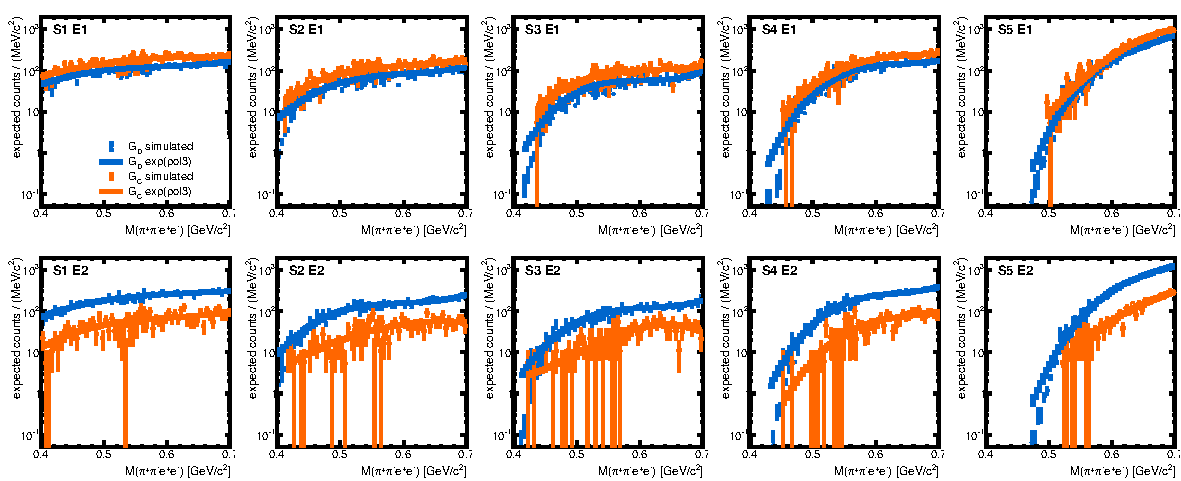
\includegraphics[width=\textwidth]{figs_all/wp3_smoothing_cnt.pdf}
\caption{Smoothing of the non-$\eta$ templates (procedure figure).
Selection: simulation only: SMASH p+p at 4.5\,GeV (standard, lepton and $\eta$ sets, mode A) at its cross sections $\times$ PDG BR $\times$ the $\eta$-decay weights V3, masses moved to the data scale ($M_4'=0.99615\,M_4$, $\Mpipi'=0.9952\,\Mpipi$), with the S0 cuts (PT3 trigger, event vertex in the target region ($\vz>-160$\,mm), \betanew particle identification (pions within $3\sigma$, leptons within $5\sigma$ and with a RICH ring), energy-loss-corrected momenta of all four tracks, all stored combinations of each event (isBest $\ge0$), both pions in the event-vertex fit); the ten histograms of the \Mpipi slices $<0.34$, 0.34--0.37, 0.37--0.39, 0.39--0.43, $\ge0.43$\,\GeVcc $\times$ \Mee$<10$ and $\ge10$\,\MeVcc, \Mfour 0.400--0.700\,\GeVcc (5\,\MeVcc bins, 2.5\,\MeVcc in 0.520--0.570); only the non-$\eta$ background groups $G_D$ (\piz Dalitz, vector-meson and other single-source pairs) and $G_C$ (conversion pairs); each fit starts at the first bin with simulated content. Points: simulated $G_D$ and $G_C$ per F10 histogram (event-group
errors); lines: the exp(pol3) smoothing, integrated over each bin. Expected raw counts per \MeVcc ($L=6079.2\,\nbinv\times63/64$); S0, SMASH
mode A, $w\times$V3. Fall-backs: E1 dropped, CR-K dropped (stage A from CR-U 0.575--0.700 only).}
\label{fig:smooth}
\end{figure}

\subsection{Step 0: the specification as written, and the E1 fall-back}
\label{sec:step0}
With E1 + E2, CR-U 0.565--0.700 and CR-K, and the data-only $\chi^2$ for the D11 rule, every extra term is added (quadratic, per-slice
tilts): $\chi^2/\mathrm{ndf}=760/297$ and $\kEone=13.19\pm0.61$. The CB factor in E1 absorbs an excess of the E1 data: data/simulation
is 1.30--1.43 in E1 against 1.12--1.29 in E2, and the fake-lepton template $T_3$ (not in the model, D6) is 26.5\,\% of $T_1+T_2$ in E1;
with the ghost variant (a) \kEone is still $8.1\pm0.6$. The fall-back ``\kEone outside 0.8--3: drop E1'' fired; every later fit
uses E2 only. The stage-A normalisation is therefore defined for \Mee$\ge10$\,\MeVcc only and is too high when carried to \Mee$<10$\,\MeVcc:
there the whole model comes out 1/0.65 too high, through its conversion scale $\kB=3.06$, where the E1 data want about 1.5--1.7 (data and
SMASH compared in $u$, \S\ref{sec:edgeu-sim}). (The second part of that fall-back, $\kappa=1\pm0.2$, concerns the signal factor of stage B; \kB stays free here.)

\subsection{Choice of the control region}
\label{sec:crchoice}
The specification requires A1 (the simulated C2--C5 below 1\,\% in every control-region bin) and A2 (a null edge step in CR-K). Three
configurations were tried, each with E2 only (Table~\ref{tab:C1}):
\begin{enumerate}\setlength{\itemsep}{0pt}
\item specification: CR-U 0.565--0.700 + CR-K (S5, 0.400--0.5225);
\item fall-back 1: CR-U from 0.575 + CR-K with \Mpipi$\ge0.44$;
\item fall-back 2: CR-U 0.575--0.700, no CR-K.
\end{enumerate}
\textbf{A1}: the largest C2--C5 share per bin is 7.7\,\% (8 of 151 bins) in configuration 1 and 6.3\,\% (5 of 136) in configuration 2,
from the radiative tail of C5 in CR-K and the bump tail near 0.565; in configuration 3 a single bin (S2E2, 0.605--0.610) holds 2.77\,\%,
which is \emph{one} simulated C2 entry ($N_{\mathrm{eff}}=1.0$); relative to the fitted model ($\aEta=0.4$) the maximum is 0.88\,\%. Integrated
over CR-U the share is 0.022\,\% (\Geta: 8.5\,\%). \textbf{A2}: in CR-K the \Mfour spectrum starts at the phase-space threshold of the
slice, right at $E(0.4116,0)=0.474$; only 15 counts lie below the edge + 2$\sigma$. An edge step fit with pol2 in 0.43--0.46 gives
$h=19.2\pm1.9$ ($\chi^2$/ndf 113/32; 23.3 with the slice's own CB) and in 0.46--0.55 $h=-0.15\pm0.97$ (Fig.~\ref{fig:crk}); a template
version gives a \emph{negative} step ($-0.35\pm0.14$ with the spread-rule CB, $-2.4\pm0.5$ with the per-cell CB), which is not an $\eta$
leak but a mis-modelled threshold. The ECAL-tagged $\eta$ in CR-K is $T=-2.1\pm4.0$ (it is zero by kinematics there), against
$3253\pm92$ in the bump region (positive control). Moreover the spread-rule CB is 46\,\% of $N$ in S5E2 ($N_{++}=2$), six times the
per-cell value. The fall-back chain ``A1 or A2 fails $\to$ CR-K at 0.44, CR-U from 0.575 $\to$ still fails $\to$ drop CR-K, take $b$ from
CR-U only, label the bump \emph{extrapolated}, add the CR-L term to S10'' fired completely.

\begin{table}[H]
\centering
\caption{Spec.\ Table~C1: candidate control regions with their content and verdict. Data S0, isBest $\ge0$, raw counts; CB spread rule;
simulation SMASH mode A, $w\times$V3. Columns: counts $N$, CB/$N$, share of the simulated C2--C5 and of \Geta, $(N-\mathrm{CB})/T_{12}$ at
SMASH. Source: WP3 (\code{wp3_tableC1.txt}). Fall-backs: CR-K at 0.44, then dropped; CR-U from 0.575.}
\label{tab:C1}
\footnotesize
\setlength{\tabcolsep}{3pt}
\resizebox{\textwidth}{!}{\tabin{fix_tC1_ra4.tex}}
\end{table}

\begin{figure}[H]
\centering
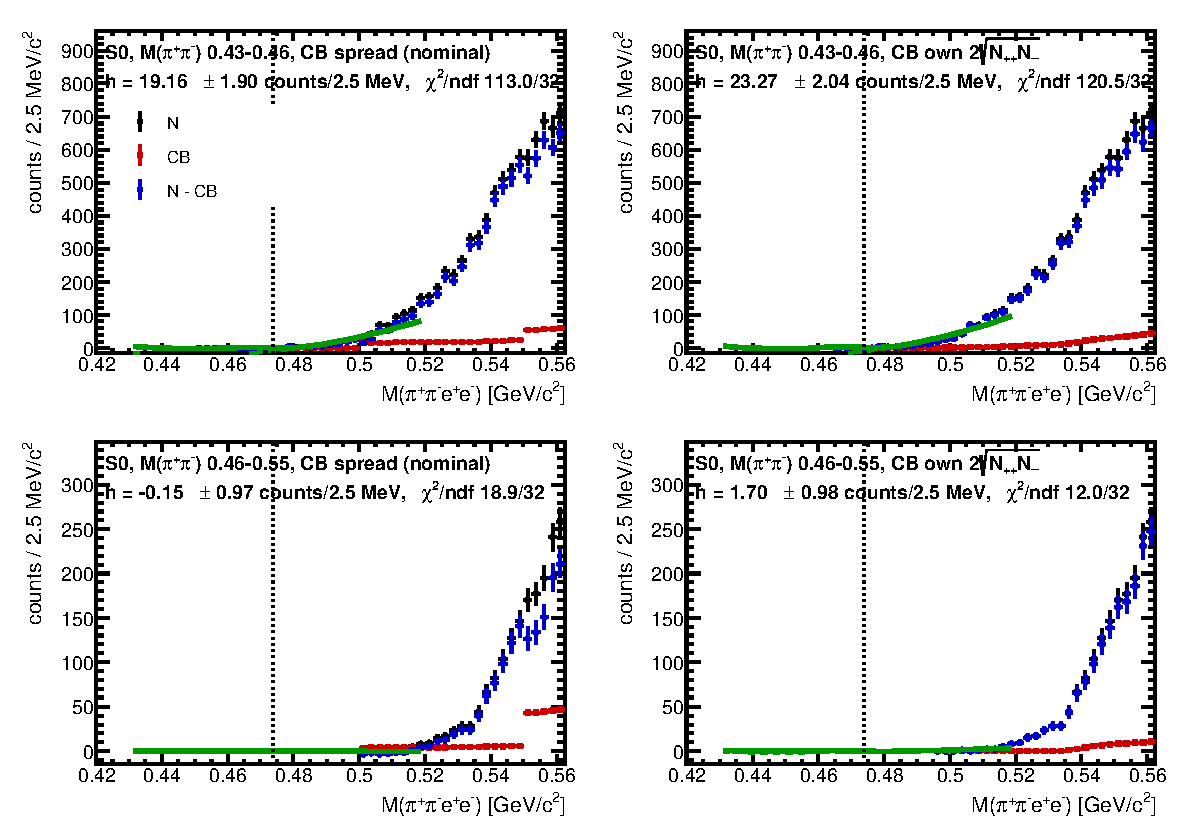
\includegraphics[width=0.85\textwidth]{figs_all/wp3_crk_edge_cnt.pdf}\\[0.2em]
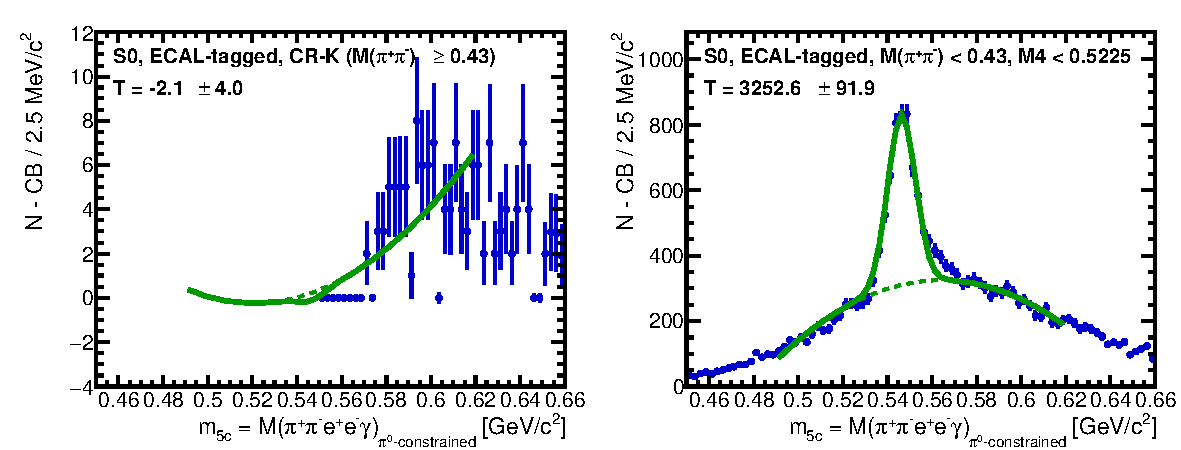
\includegraphics[width=0.85\textwidth]{figs_all/wp3_crk_tag.pdf}
\caption{Test A2 in CR-K.
Selection: data, S0 (PT3 trigger, event vertex in the target region ($\vz>-160$\,mm), \betanew particle identification (pions within $3\sigma$, leptons within $5\sigma$ and with a RICH ring), energy-loss-corrected momenta of all four tracks, all stored combinations of each event (isBest $\ge0$), both pions in the event-vertex fit), all \Mee. Top: \Mpipi 0.43--0.46\,\GeVcc (upper row) and 0.46--0.55\,\GeVcc (lower row), \Mfour in 2.5\,\MeVcc bins; pol2 + a step at the fixed edge 0.4739\,\GeVcc (smeared by 5.4\,\MeVcc) fitted over the edge $\pm45$\,\MeVcc; CB $=2\sqrt{N_{++}N_{--}}$ (10\,\MeVcc cells, $k=1$) of all slices shared out by the like-sign share of each 50\,\MeVcc band (left) or of the slice itself (right). Bottom: ECAL-tagged counts, a good ECAL photon (photon identification, $0.8<\beta<1.2$, energy above 100\,MeV; of several the one with $M(\ee\gamma)$ closest to 0.140\,\GeVcc) with $0.119\le M(\ee\gamma)<0.173$\,\GeVcc and \Mee$<0.10$\,\GeVcc; m5c ($M(\pipi\ee\gamma)$, photon energy rescaled to $M(\ee\gamma)=m_{\piz}$) fitted in 0.49--0.62\,\GeVcc (CB in 20\,\MeVcc cells) with a fixed Gaussian (0.5463\,\GeVcc, 6.2\,\MeVcc) + pol2; left \Mpipi$\ge0.43$\,\GeVcc and \Mfour 0.400--0.5225\,\GeVcc, right \Mpipi$<0.43$\,\GeVcc and \Mfour$<0.5225$\,\GeVcc. Top: $N$ (black), CB (red) and $N-\mathrm{CB}$ (blue) in the CR-K slices 0.43--0.46 and 0.46--0.55\,\GeVcc, S0,
raw counts per 2.5\,\MeVcc; green: pol2 + step fit with the step at $E(0.4116,0)=0.4739$ (dotted); left the spread-rule CB, right the CB of
the slice itself. The data are empty below the phase-space threshold of each slice (about 0.47 and 0.50), so the step absorbs the
threshold. Bottom: ECAL-tagged $\eta$, $N-\mathrm{CB}$ in the \Mfour with the photon (m5c); left CR-K ($T=-2.1\pm4.0$), right
\Mpipi$<0.43$, \Mfour$<0.5225$ ($T=3253\pm92$, positive control). Fall-back: CR-K dropped after this test.}
\label{fig:crk}
\end{figure}

\subsection{The background model (D11) with the template covariance}
\label{sec:d11}
D11 adds a quadratic term, then per-slice tilts, if $\Delta\chi^2>4$. With the data-only $\chi^2$ every term is added, but the templates
are 10--50 times less precise than the data in CR-U, so the data-only $\Delta\chi^2$ rewards terms that follow template fluctuations (for
example an $\omega$ split gives $c_\omega=3.4\pm0.5\,(\mathrm{stat})\pm2.2\,(\mathrm{MC})$). WP3 therefore evaluated D11 with a GLS
$\chi^2$: data variance + MC covariance of the predicted spectrum (100 replicas, 3 iterations), as in the simulation-study fits behind
D11's ``3.8 $\to$ 1.3''. In fall-back 2 (125 bins):

\begin{table}[H]
\centering
\caption{Nested stage-A models in the adopted configuration (CR-U 0.575--0.700, E2). GLS: $\chi^2$ with the template covariance. The
full table for all four configurations is Table~\ref{tab:C2}. Fall-backs: E1 dropped, CR-K dropped (stage A from CR-U 0.575--0.700 only).}
\label{tab:d11}
\small
\begin{tabular}{@{}l r r r@{}}
\toprule
model & GLS $\chi^2$/ndf & GLS $\Delta\chi^2$ & data-only $\chi^2$/ndf \\
\midrule
M0 scale $c_j$ only & 138.8/119 & -- & 443.4/119 \\
\textbf{M1 + common tilt (adopted)} & \textbf{129.8/118} & 9.0 & 326.4/118 \\
M2 + quadratic & 127.9/117 & 1.9 & 252.3/117 \\
M3 per-slice tilts & 127.5/114 & 2.4 & 271.8/114 \\
\bottomrule
\end{tabular}
\end{table}

M1 is adopted, $\chi^2/\mathrm{ndf}=1.10$ (GLS). \flag{Deviation: D11 and the criterion $\chi^2/\mathrm{ndf}\le1.5$ were evaluated with
the template covariance; with the data-only $\chi^2$ the chain ends at per-slice tilts + quadratic + $\omega$ split, $\chi^2$ 139.0/112;
this choice is kept as the family-S3 variants ``D11data'' and ``D11data+omega''.} The parameter values come from the specified estimator
(Poisson likelihood with the data variance); the GLS values agree within the MC error.

\textbf{Check with the hybrid covariance (review).} WP3's GLS uses the sample covariance of 100 replica predictions, which has rank $\le99$
for 125 bins; the verifier v5 showed for F-main that this construction is not converged. The review recomputed stage A with v5's hybrid
covariance (data + the exact diagonal variance of the fixed raw $\eta$ templates + the replica covariance of the smoothed background,
rank 36, converged: 50 and 100 replicas agree to 0.3\,\%), with v5's smoothing (WP4 smoothing, about 3.5\,\% different from WP3's on $c_j$),
\code{plots/all_report/fix_stageA_gls.py}:
\begin{center}\footnotesize
\resizebox{\textwidth}{!}{%
\begin{tabular}{@{}l r r r r@{}}
\toprule
$\eta$ terms fixed at & data only & GLS-rep (WP3) & GLS-hyb & $\Delta\chi^2_{\mathrm{hyb}}$: M0$\to$M1 / M1$\to$M2 / M1$\to$M3 \\
\midrule
WP3 ($a=0.4$, $g=1$) & 412.5/118 & 144.1/118 $=1.22$ & 143.3/118 $=1.21$ & 3.5 / \textbf{4.2} / 2.1 \\
F-main ($a=0.382$, $g=1.72$) & 429.9/118 & 150.7/118 $=1.28$ & 146.2/118 $=1.24$ & 3.2 / \textbf{4.5} / 2.1 \\
\bottomrule
\end{tabular}}
\end{center}
The criterion $\chi^2/\mathrm{ndf}\le1.5$ passes with the hybrid covariance (1.21--1.24); the per-slice tilts are not needed (A4: $p=0.72$).
But with this covariance the quadratic term is just above the D11 threshold ($\Delta\chi^2=4.2$--4.5 against 4), so the D11 choice of M1 is
\textbf{borderline}. The quadratic variant is family S3 (B4 $+150$\,\%, peak side bands $+3.4$\,\%, F-main \aEta $+39$\,\%), so the main
peak result is not affected beyond its S3 entry, and the B4 bump area, which it moves most, is not determined anyway (D23, approved); the bump measured
through its edge moves by only $-2.1$\,\% (\S\ref{sec:bedge-toys}).

\begin{table}[H]
\centering
\caption{Spec.\ Table~C2: nested stage-A models in the four configurations ($\chi^2$/ndf with the data variance; in brackets with the template
covariance, GLS; bold: chosen by D11 in that configuration) and the adopted parameters (model M1, E2, CR-U 0.575--0.700, S0,
$\aEta^{(0)}=0.4$): value, statistical (sandwich), MC (100 replicas) and total error, and the derivative with respect to $\aEta^{(0)}$.
Source: WP3 (\code{wp3_tableC2.txt}, \code{stageA.txt}). Fall-backs: E1 dropped, CR-K dropped (stage A from CR-U 0.575--0.700 only).}
\label{tab:C2}
\small
\tabin{wp3_tableC2.tex}
\end{table}

Correlations (total): $c_j$--$c_k$ 0.97--0.98, $c_j$--\kB $-0.91$ to $-0.93$: in E2 the shapes of $G_D$ and $G_C$ are similar, so only
their sum is constrained; the background per bin, $B_A$, is much better known than $c_j$ or \kB separately. Event groups change the
errors by 0.2--0.7\,\%; the CB replicas give 0.007--0.009 on $c_j$. At $\aEta^{(0)}=0$, 1 and 2 the factors $c_1$ are 1.007, 0.944, 0.866
and $b=-0.0696$, $-0.0669$, $-0.0606$; the GLS $\chi^2$ rises from 129.8 at $\aEta^{(0)}=0.4$ to 153.4 at 1, i.e.\ the control region
itself prefers a small $\eta$ scale (through \Geta, 8.5\,\% of CR-U E2 at SMASH).

\subsection{Tests A1--A5}
\begin{table}[H]
\centering
\caption{Acceptance tests of stage A (specification WP3) for the adopted configuration. Source: WP3 (\code{wp3_acceptance.txt}). Fall-backs: E1 dropped, CR-K dropped (stage A from CR-U 0.575--0.700 only).}
\label{tab:A15}
\small
\begin{tabular}{@{}p{5.4cm} p{6.6cm} p{3.4cm}@{}}
\toprule
test & value & verdict \\
\midrule
$\chi^2/\mathrm{ndf}\le1.5$ & GLS $129.8/118=1.10$ (data only 2.77); hybrid GLS 1.21 (review); WP6 rerun at the F-main $\eta$: 1.46/1.56 without the $\eta$-template variance, 1.24 hybrid & PASS, borderline (data-only: FAIL) \\
A1: C2--C5 $<1$\,\% in every CR bin & one bin 2.77\,\% (one simulated entry); relative to the model 0.88\,\% & literal FAIL; PASS against the fitted model \\
A2: CR-K edge step $|h|<2\sigma$ & 0.43--0.46: 10$\sigma$ (pol2 cannot describe the threshold); 0.46--0.55: $-0.15\pm0.97$ & FAIL (ill-posed) / PASS \\
A2: tagged $\eta$ in CR-K $=0$ & $T=-2.1\pm4.0$ (zero by kinematics) & PASS (trivially) \\
A3: $\eta$ injected $\times\{0,0.4,1,2\}$ moves $c_j$, $b$ by $<0.3\sigma$ & C2--C5: 0.045$\sigma$; with \Geta also injected 0.68$\sigma$ (\Geta is 8.5\,\% of CR-U at SMASH, 4.7\,\% of $N-\mathrm{CB}$ at $ag=0.656$) & PASS for C2--C5; \textbf{FAIL} for the $\eta$-related content (\Geta) \\
A4: per-slice tilts consistent with a common $b$ & GLS $\Delta\chi^2=2.38/4$, $p=0.67$; hybrid 2.1/4, $p=0.72$ (data only $p=4\times10^{-11}$) & PASS (with the template covariance) \\
A4: CR-U split at \Mpipi$=0.42$ & data/model $1.0010\pm0.0138$ vs $1.0013\pm0.0152$ ($-0.02\sigma$) & PASS \\
A5: K$^0_S$ veto 0.485--0.507 moves the parameters by $<1\sigma$ & largest 0.68$\sigma$ (\kEtwo) & PASS \\
\bottomrule
\end{tabular}
\end{table}

\subsection{The renormalised background: figures and the counted ``after'' display}
\begin{figure}[H]
\centering
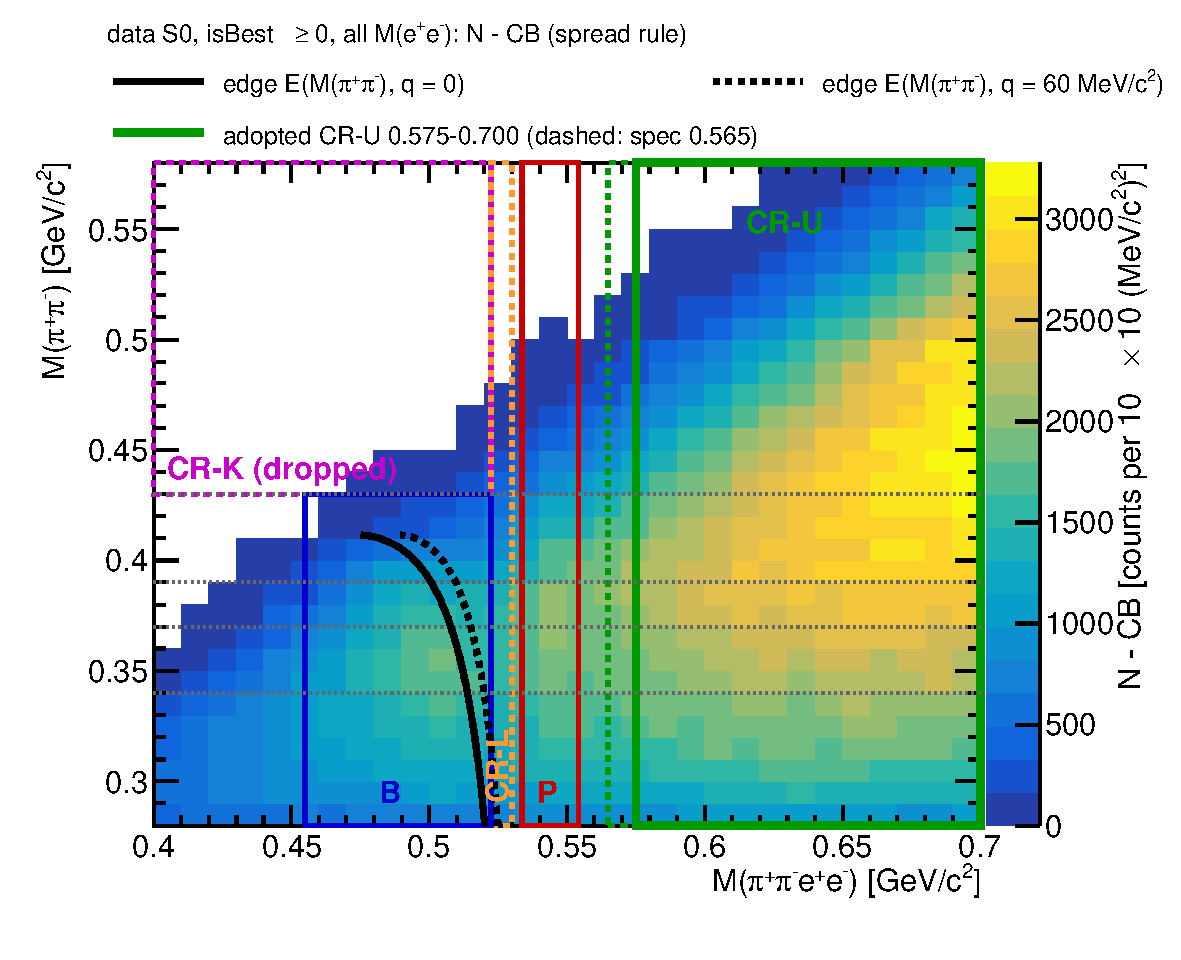
\includegraphics[width=0.75\textwidth]{figs_all/wp3_map_cnt.pdf}
\caption{Spec.\ Fig.~C1: data $N-\mathrm{CB}$ in the plane \Mfour$\times$\Mpipi, S0, isBest $\ge0$, all \Mee; raw counts per
$10\times10$\,(\MeVcc)$^2$; CB $=2\sqrt{N_{++}N_{--}}$, spread rule.
Selection: data only, S0 (PT3 trigger, event vertex in the target region ($\vz>-160$\,mm), \betanew particle identification (pions within $3\sigma$, leptons within $5\sigma$ and with a RICH ring), energy-loss-corrected momenta of all four tracks, all stored combinations of each event (isBest $\ge0$), both pions in the event-vertex fit), all \Mee; \Mfour 0.40--0.70\,\GeVcc and \Mpipi 0.28--0.58\,\GeVcc in $10\times10$\,(\MeVcc)$^2$ cells; CB $=2\sqrt{N_{++}N_{--}}$ of the like-sign data with the same cuts (10\,\MeVcc cells of \Mfour, $k=1$), shared out to the \Mpipi cells by the like-sign share of each 50\,\MeVcc band. Boxes: CR-U adopted from 0.575 (thick green; the specification's
0.565 thin), CR-K (\Mpipi$\ge0.43$, \Mfour$<0.5225$, magenta, dropped), CR-L (orange), bump window B (blue) and peak window P (red).
Lines: $E(m,q)$ for $q=0$ (solid) and 60\,\MeVcc (dotted); dotted horizontal lines: slice boundaries. No simulation. Fall-backs: CR-K
dropped, CR-U from 0.575 (A1/A2).}
\label{fig:C1}
\end{figure}

\begin{figure}[H]
\centering
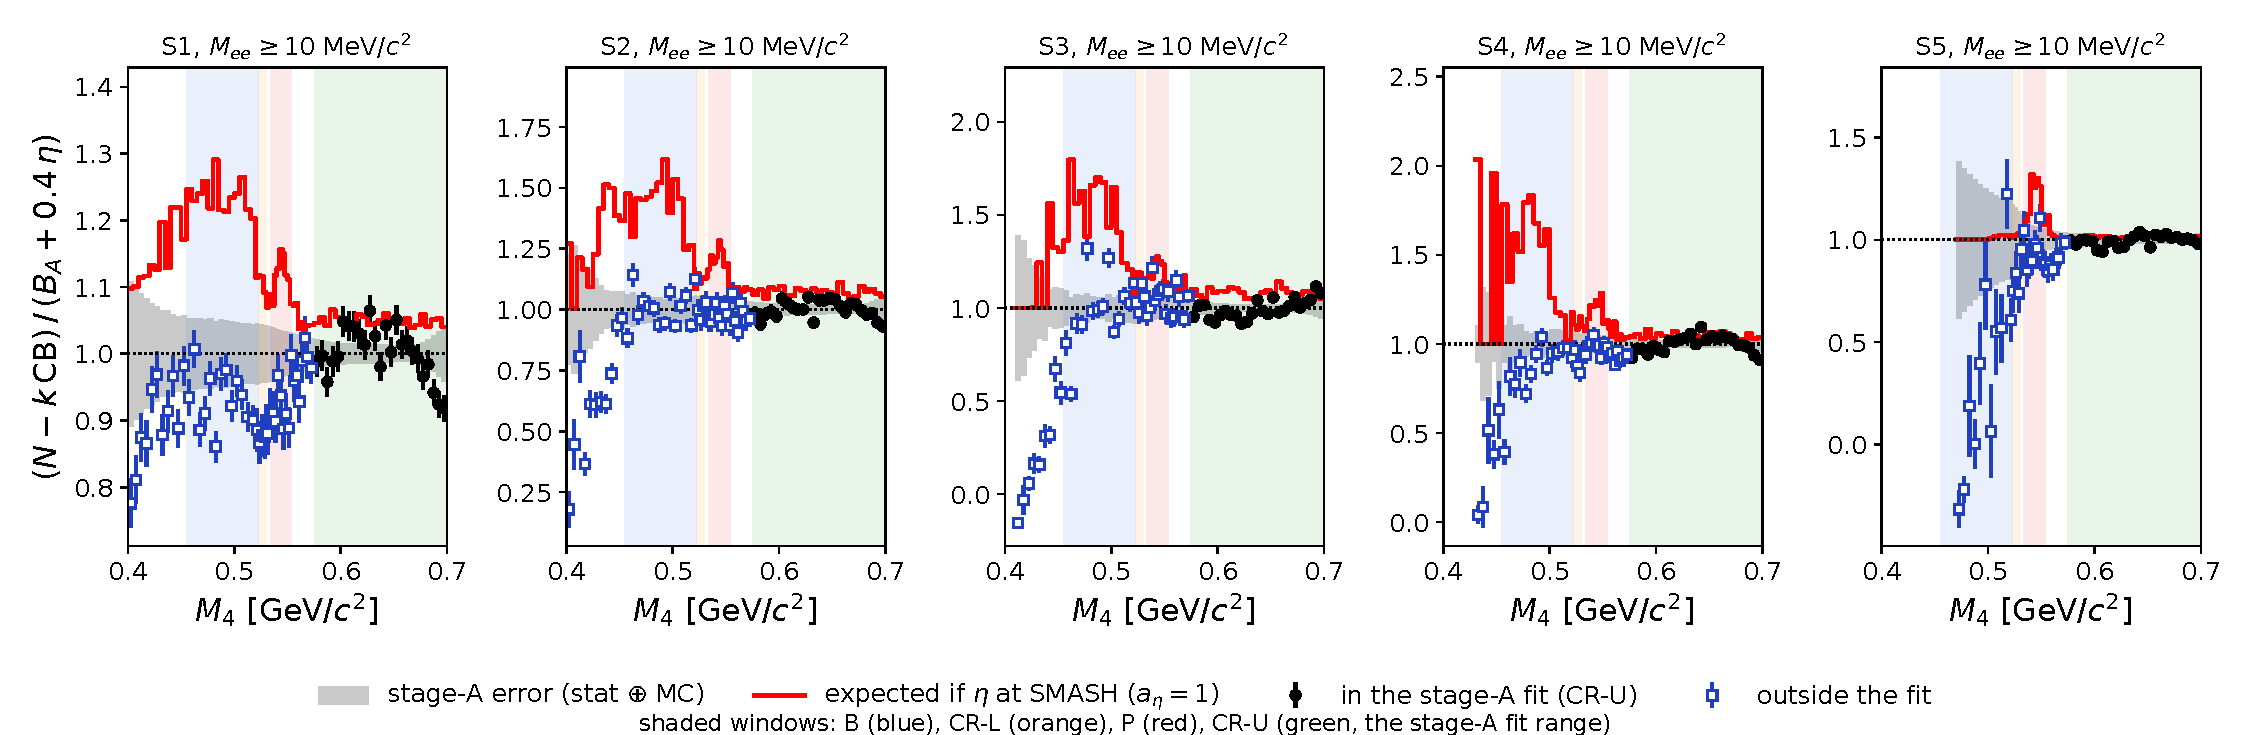
\includegraphics[width=\textwidth]{figs_all/fix_C2.pdf}
\caption{Spec.\ Fig.~C2: per slice S1--S5, \Mee$\ge10$\,\MeVcc: $(N-k\,\mathrm{CB})/(B_A+0.4\,\eta)$, $k=k_{E2}=0.954$, with $B_A$ the frozen
stage-A background and $\eta$ all $\eta$ classes at SMASH $\times$ PDG BR (raw counts on both sides of the ratio).
Selection: data, S0 (PT3 trigger, event vertex in the target region ($\vz>-160$\,mm), \betanew particle identification (pions within $3\sigma$, leptons within $5\sigma$ and with a RICH ring), energy-loss-corrected momenta of all four tracks, all stored combinations of each event (isBest $\ge0$), both pions in the event-vertex fit); \Mee$\ge10$\,\MeVcc; one panel per slice (the \Mpipi slices $<0.34$, 0.34--0.37, 0.37--0.39, 0.39--0.43, $\ge0.43$\,\GeVcc); \Mfour 0.400--0.700\,\GeVcc (5\,\MeVcc bins, 2.5\,\MeVcc in 0.520--0.570); CB $=2\sqrt{N_{++}N_{--}}$ of the like-sign data with the same cuts (10\,\MeVcc cells of \Mfour, $k=1$), shared out by the like-sign share of each 50\,\MeVcc band, times $k=0.954$; $B_A$: smoothed SMASH $G_D+\kB G_C$ renormalised by the stage-A fit in \Mfour 0.575--0.700\,\GeVcc, \Mee$\ge10$\,\MeVcc; $\eta$: C2+C3+C4+C5+\Geta; SMASH p+p at 4.5\,GeV (standard, lepton and $\eta$ sets, mode A) at its cross sections $\times$ PDG BR $\times$ the $\eta$-decay weights V3, masses moved to the data scale ($M_4'=0.99615\,M_4$, $\Mpipi'=0.9952\,\Mpipi$), same cuts. Black full circles: bins of
the stage-A fit (CR-U 0.575--0.700, green shading); blue open squares: outside the fit. Grey band: $\pm$ stage-A error (stat $\oplus$ MC).
Red: the ratio expected if the $\eta$ were at SMASH ($\aEta=1$) instead of 0.4. Bins below the kinematic threshold of a slice (no model
content) are not drawn; each panel has its own $y$ range, which contains every point. S0, isBest $\ge0$; SMASH mode A, $w\times$V3.
Fall-backs: E1 dropped, CR-K dropped (stage A from CR-U only). Redrawn from WP3's \code{stageA.root} (\code{fix_after.py}).}
\label{fig:C2}
\end{figure}

\begin{figure}[!htbp]
\centering
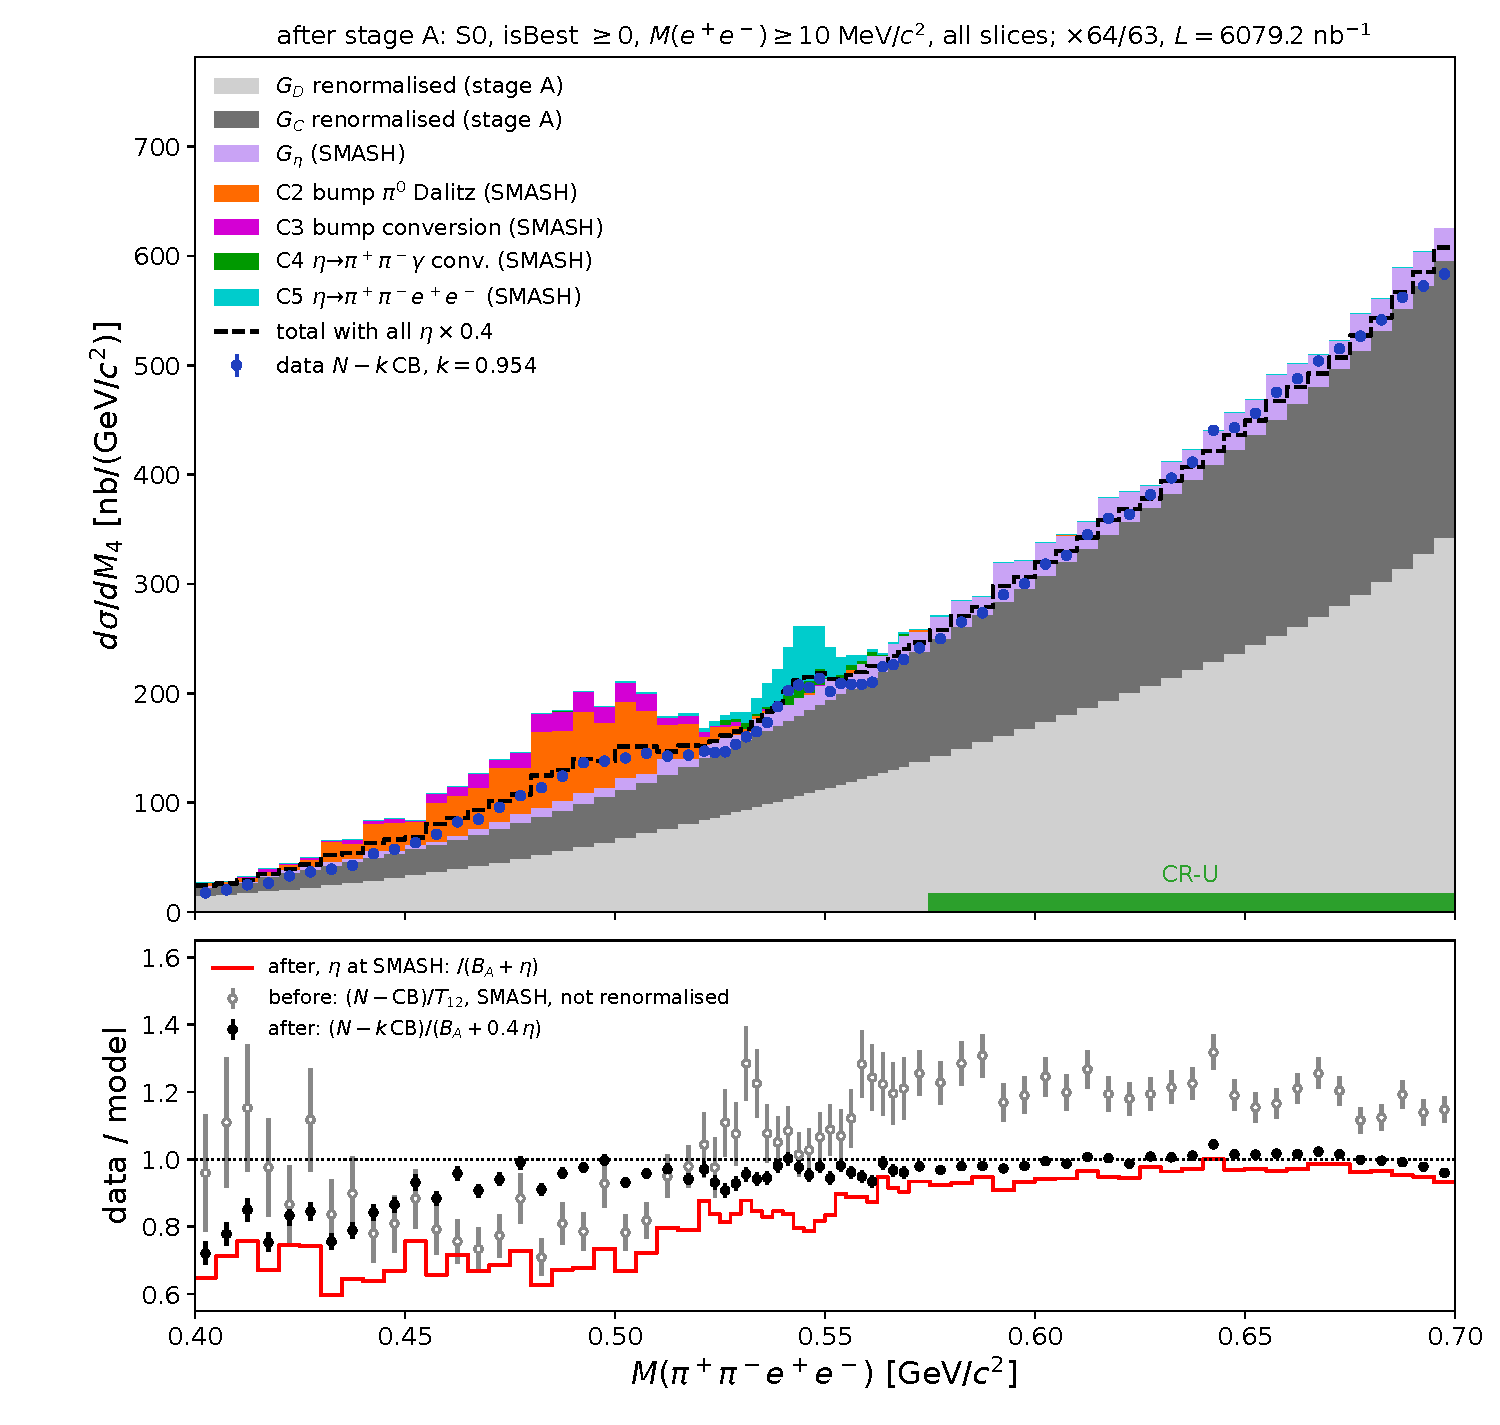
\includegraphics[width=0.78\textwidth]{figs_all/fix_C3.pdf}
\caption{Spec.\ Fig.~C3: ``after'' spectrum, \Mee$\ge10$\,\MeVcc, all slices, in the common colours.
Selection: data, S0 (PT3 trigger, event vertex in the target region ($\vz>-160$\,mm), \betanew particle identification (pions within $3\sigma$, leptons within $5\sigma$ and with a RICH ring), energy-loss-corrected momenta of all four tracks, all stored combinations of each event (isBest $\ge0$), both pions in the event-vertex fit); \Mee$\ge10$\,\MeVcc; the five \Mpipi slices summed; \Mfour 0.400--0.700\,\GeVcc (5\,\MeVcc bins, 2.5\,\MeVcc in 0.520--0.570); after: CB $=2\sqrt{N_{++}N_{--}}$ of the like-sign data with the same cuts (10\,\MeVcc cells of \Mfour, $k=1$), shared out by the like-sign share of each 50\,\MeVcc band, times $k=0.954$, and SMASH $G_D$, $G_C$ renormalised by the stage-A fit in \Mfour 0.575--0.700\,\GeVcc (\Mee$\ge10$\,\MeVcc); before: CB with $k=1$ and SMASH $T_1+T_2$ not renormalised; SMASH p+p at 4.5\,GeV (standard, lepton and $\eta$ sets, mode A) at its cross sections $\times$ PDG BR $\times$ the $\eta$-decay weights V3, masses moved to the data scale ($M_4'=0.99615\,M_4$, $\Mpipi'=0.9952\,\Mpipi$), same cuts. Data $N-k\,\mathrm{CB}$ (blue) as
$d\sigma/dM_4$, $\times64/63$/6079.2\,\nbinv. Stack: renormalised $G_D$ (light grey) and $G_C$ (dark grey) of stage A; \Geta (violet), C2
(orange), C3 (magenta), C4 (green), C5 (cyan) at SMASH $\times$ PDG BR ($\aEta=1$); dashed: total with all $\eta$ $\times0.4$. Ratio panel:
\emph{after} $=(N-k\,\mathrm{CB})/(B_A+0.4\,\eta)$ (black), the same with $\eta$ at SMASH (red line), and \emph{before} $=(N-\mathrm{CB})/T_{12}$
with SMASH not renormalised (grey open circles; same class E2, same unit), so the two can be compared directly (Table~\ref{tab:C3ba}). Green
bar: CR-U. In E2, $G_D$ and $G_C$ cannot be separated (correlation of \kB and $c_j$ $-0.92$). Display, not a yield (D20). Fall-backs: E1 and
CR-K dropped. Redrawn (\code{fix_after.py}).}
\label{fig:C3}
\end{figure}

\begin{table}[H]
\centering
\caption{Spec.\ Table~C3: counted ``after'' display in the regions of Table~\ref{tab:B1}, data S0, \Mee$\ge10$\,\MeVcc, raw counts. $B_A$: stage-A
background (stat $\oplus$ MC); $\eta$ (SMASH): all $\eta$ classes at $\aEta=1$; ratio $=(N-k\,\mathrm{CB})/(B_A+0.4\,\eta)$. These are
display counts, not yields (D20). Source: WP3 (\code{wp3_tableC3.txt}). Fall-backs: E1 and CR-K dropped.}
\label{tab:C3}
\small
\resizebox{\textwidth}{!}{\tabin{fix_tC3.tex}}
\end{table}

\begin{table}[H]
\centering
\caption{Before and after the renormalisation on the same footing: class E2, all slices, S0, raw counts, the regions of Table~\ref{tab:C3}.
Before $=(N-\mathrm{CB})/T_{12}$ (SMASH, no renormalisation, $k=1$); after $=(N-k\,\mathrm{CB})/(B_A+0.4\,\eta)$ (WP3). Source:
\code{tables_all/fix_tableC3_before.txt} (\code{fix_after.py}; the ``after'' column is reproduced exactly).}
\label{tab:C3ba}
\small
\begin{tabular}{@{}l r r@{}}
\toprule
region [\GeVcc] & before (E2) & after (E2) \\
\midrule
R0$'$ 0.400--0.455 & $0.899\pm0.035$ & $0.828\pm0.050$ \\
R1 $=$ B 0.4550--0.5225 & $0.833\pm0.017$ & $0.952\pm0.038$ \\
R2 0.5225--0.5336 & $1.116\pm0.045$ & $0.932\pm0.036$ \\
R3 $=$ P 0.5336--0.5542 & $1.066\pm0.025$ & $0.969\pm0.028$ \\
R4 0.5542--0.565 & $1.203\pm0.043$ & $0.960\pm0.023$ \\
R5 0.565--0.700 & $1.197\pm0.009$ & $0.998\pm0.006$ \\
CR-U 0.575--0.700 & $1.196\pm0.010$ & $0.999\pm0.006$ \\
CR-L 0.5225--0.5300 & $1.051\pm0.054$ & $0.923\pm0.037$ \\
\bottomrule
\end{tabular}
\end{table}

In E2 the renormalisation brings CR-U from 1.20 to 1.00 by construction; the bump window moves from 0.83 to 0.95 and the peak window from 1.07
to 0.97, while the region below the bump moves from 0.90 to 0.83: the background carried down from CR-U is too high there (\S\ref{sec:closure}).
The ``before'' column here (E2 only) differs from Table~\ref{tab:B1} (all \Mee, cross-section units).

\textbf{Reading.} The stage-A background overshoots the data below the bump: in 0.400--0.455 the background alone exceeds
$N-k\,\mathrm{CB}$ (12\,897 against 12\,407 counts; ratio 0.83 with 0.4 $\eta$), CR-K is low (pull $-3.0$) and CR-L low by 1.1$\sigma$.
In the bump window the display gives $N-k\,\mathrm{CB}-B_A=8895\pm2012$ counts against $0.4\times\eta(\mathrm{SMASH})=11316$; this is not a
yield. The extrapolation of the background 40--120\,\MeVcc below CR-U into B is the weak point of the bump measurement; stage B keeps the
background free (\S\ref{sec:fit}) and the closure tests of \S\ref{sec:closure} quantify it.

\subsection{Variants and closure of stage A}
\begin{table}[H]
\centering
\caption{Stage-A variants (same model and control region unless stated; values only, the errors are in \code{stageA.txt}). $\chi^2$ with the data
variance only. Fall-backs: E1 dropped, CR-K dropped (stage A from CR-U 0.575--0.700 only).}
\label{tab:stageAvar}
\small
\begin{tabular}{@{}l r r r r r@{}}
\toprule
variant & $\chi^2$/ndf & $c_1$ & $c_5$ & $b$ & \kB \\
\midrule
adopted & 326.4/118 & 0.988 & 0.909 & $-0.068$ & 3.06 \\
CR-U 0.565--0.700 & 349.7/133 & 0.958 & 0.885 & $-0.064$ & 3.24 \\
specification CRs (+ CR-K) & 403.5/148 & 0.920 & 0.855 & $-0.065$ & 3.56 \\
fall-back 1 (CR-K, \Mpipi$\ge0.44$) & 375.1/133 & 0.930 & 0.865 & $-0.071$ & 3.53 \\
$\kB=1\pm0.2$ & 369.6/119 & 1.184 & 1.056 & $-0.061$ & 1.94 \\
CB per-cell geometric mean (S1) & 296.4/118 & 1.053 & 0.980 & $-0.070$ & 2.56 \\
ghost variant (a) & 295.1/118 & 0.887 & 0.857 & $-0.084$ & 2.78 \\
K$^0_S$ veto (A5) & 350.8/118 & 0.971 & 0.940 & $-0.073$ & 3.19 \\
D11 data-only (per-slice tilts + quadratic) & 186.0/113 & 1.023 & 0.831 & per slice & 2.29 \\
D11 data-only + $\omega$ split ($c_\omega=3.36$) & 139.0/112 & 0.831 & 0.671 & per slice & 2.68 \\
``pre'' (parallel column) & 607.5/118 & 1.212 & 1.110 & $-0.088$ & 2.52 \\
step 0: E1+E2, \kEone free & 760.1/297 & 1.243 & 0.979 & per slice & 0.95 \\
\bottomrule
\end{tabular}
\end{table}

\textbf{Closure.} The adopted (frozen WP3) fit predicts CR-L (E2) as $8078\pm522$ counts against 7519 observed (pull $-1.06$) and CR-K as
$440\pm32$ against 331 (pull $-3.0$); WP6's rerun of stage A at the F-main $\eta$ values gives $-1.88$, $-1.98$ and, below the bump,
$-2.78$ (Table~\ref{tab:bclos}). The CR-L term, $\max(|\mathrm{pred}-\mathrm{obs}|,\sigma_{\mathrm{pred}})=559$ counts (8.4\,\% of $N-k\,\mathrm{CB}$),
is the family-S10 entry required by the fall-back; WP6 recomputed it with stage A at the fitted $\eta$ values (\S\ref{sec:closure}).

%======================================================================
\section{Validation of the estimators on simulation (stress closure)}
\label{sec:val}
%======================================================================
\inshort{on simulated pseudo-data with a known truth only the peak side-band estimator recovers the truth within the allowed bias, under the rule adopted during the analysis (D22; under the specification's configuration every estimator fails). The template fits are biased by about $-10$\,\% and become cross-checks; the bump estimator B4 fails marginally.}
\notebox{\textbf{Verdict} (WP4, decided before any data yield was quoted, D20). \textbf{Only the peak side-band estimator passes, under the
adopted rule} (method configurations AA/BB + RF). \textbf{Deviation, approved by the analyst on 15 November 2026 (D22)}: the specification's configuration BA is not the
gate; under BA \emph{every} estimator fails, the peak side bands included ($+9.9$\,\% in (a), $+14$\,\% in b$-$, $+16.8$\,\% in (f)), and the
RF gate was adopted after the BA results were seen (BA carries four times the template noise of the real analysis, \S\ref{sec:val}). With the
bias correction (RB) the peak side bands are ``FAIL marginal'' (coverage 0.57 in (h)). B4 (bump side bands) fails marginally (a bias of
$-5.8$\,\% against the 5\,\% tolerance in the $\omega$ scenario) and passes with RB. F-main, F-free and F-gold fail: their raw signal templates
bias them by about $-10$\,\% (F-gold \BRG $+15$\,\%), and their template-statistics error is 1.6--3.6 times the statistical error. By the
fall-back of the specification the template fits are cross-checks, and B4 + the peak side bands are the main estimators.}

\subsection{What was tested}
\textbf{Pseudo-data (toys).} Each toy is a data set at $L=6079.2\,\nbinv$ (raw counts, S0, isBest $\ge0$) whose truth is known:
\begin{enumerate}\setlength{\itemsep}{0pt}
\item the CB of the data, built again in every toy from Poisson-fluctuated like-sign counts per (2.5\,\MeVcc bin, slice, \Mee class) with
      the WP0 spread rule (it reproduces the factory CB to $3.5\times10^{-16}$);
\item plus the smoothed simulated non-$\eta$ background times $c\,(1+bx)$, the tilt integrated exactly over each cell;
\item plus $\aEta\,[\mathrm{C2}+\kappa(\mathrm{C3}+\mathrm{C4})+\rhod\,\mathrm{C5}+g\,\Geta]$ from the raw simulated entries;
\item the toy $N$ is a Poisson draw of this truth in every cell. The cells are the F10 bins split at every window edge (77 \Mfour cells
      $\times$ 5 slices $\times$ 3 \Mee classes), so every window of every estimator is an exact sum.
\end{enumerate}
\textbf{Scenarios} (truth relative to the fit model): (a) background $\times1.35$, tilt $-0.15$, $\aEta=0.4$, $\rhod=\kappa=g=1$;
(b$\pm$) $\rhod=0.5/1.5$; (c$\pm$) $\kappa=0.8/1.2$; (d$\pm$) $g=0.5/1.5$; (e) background with $\omega/\rho^0$ pions $\times0.3$ and the rest
$\times1.6$; (f) truth with $s+0.0009$ and $r_{\mathrm{res}}=0.89$, templates nominal; (g) $\aEta=0$; (h) $\aEta=1$; (i, information) true CB
distributed like the per-cell geometric mean. 500 toys per scenario and configuration.

\textbf{Configurations.} \textbf{BA} (the specification): truth from half B of the simulation, templates from half A; \textbf{AB} the swap;
\textbf{AA, BB} (``method''): truth and templates from the same half; \textbf{RF} (``realistic MC''): truth from the full sample, toy $t$
fitted with the templates of bootstrap replica $t$ mod 100, so the template-to-truth difference has exactly the noise of the real analysis;
\textbf{RB}: RF with a bootstrap bias correction (estimate $=2\,v-$ mean of 20 child replicas). The fitter is Fisher scoring with
variance $\max(\mu,1)+k^2\mathrm{var(CB)}+$ BB-lite; errors are sandwich errors ($\oplus\sigma_{\mathrm{MC}}$ in RF/RB). About 160\,000
estimator chains were run; no F-main, F-free, stage-A or side-band fit failed (F-gold: 3 of 500 in one configuration).

\textbf{Criteria} (specification): $|\mathrm{bias}|<\max(0.5\sigma_{\mathrm{stat}},f\,|\mathrm{true}|)$ with $f=5$\,\% (\aEta, \Ybump),
10\,\% (\Ypeak), 20\,\% (\rhod, BR); 68\,\% coverage 0.60--0.76 (required where the model contains the truth: a--d, g, h); null scenario
$|$mean pull$|<0.5$; at most 1\,\% failed fits. \textbf{Decision rule} (fixed before the RB run): an estimator passes if it passes both
method configurations and RF; ``with bias correction'' uses RB instead of RF; ``FAIL marginal'' means every failed criterion lies within
2$\sigma$ of its limit.

\flag{Deviation: the BA configuration of the specification is reported but not used as the gate.} The two halves of the smoothed
background differ by 5--10\,\% per 50\,\MeVcc band (MC statistics), and this single realisation alone moves \aEta by $+32$\,\% (BA) or
$-37$\,\% (AB) and B4 by $+27$/$-31$\,\%: the template-to-truth difference has four times the variance of the real analysis. When truth and
templates come from the same half (AA, BB) the method closes exactly (Asimov bias below 0.03\,\%, $\chi^2=0$). RF is the closest sound test
with the same intent.

\subsection{Results}
\begin{table}[H]
\centering
\caption{Spec.\ Table~V1: stress closure. Columns 3--5: statistical error, template-statistics error and mean replica shift in the realistic
configuration RF, scenario (a); columns 6--10: bias in scenario (a) per configuration (RF+BC $=$ RB); 11--13: largest bias over (a)--(h)
(scenario in brackets); 14--17: verdicts (``fail (m)'': within 2$\sigma$ of the limit). All in per cent of the true value (RF (a): \aEta
0.4, \Ybump 21\,904, \Ypeak 4\,866 counts). Precision of the biases: 0.1\,\% (BA, AB, AA, BB), 0.4--1\,\% (RF, RB). S0, isBest $\ge0$,
$L=6079.2\,\nbinv$, 500 toys per point. Source: WP4 (\code{wp4_V1.txt}). Fall-back consequence: estimators that fail are cross-checks only.}
\label{tab:V1}
\scriptsize
\setlength{\tabcolsep}{2pt}
\resizebox{\textwidth}{!}{\tabin{wp4_V1.tex}}
\end{table}

\begin{figure}[!tbp]
\centering
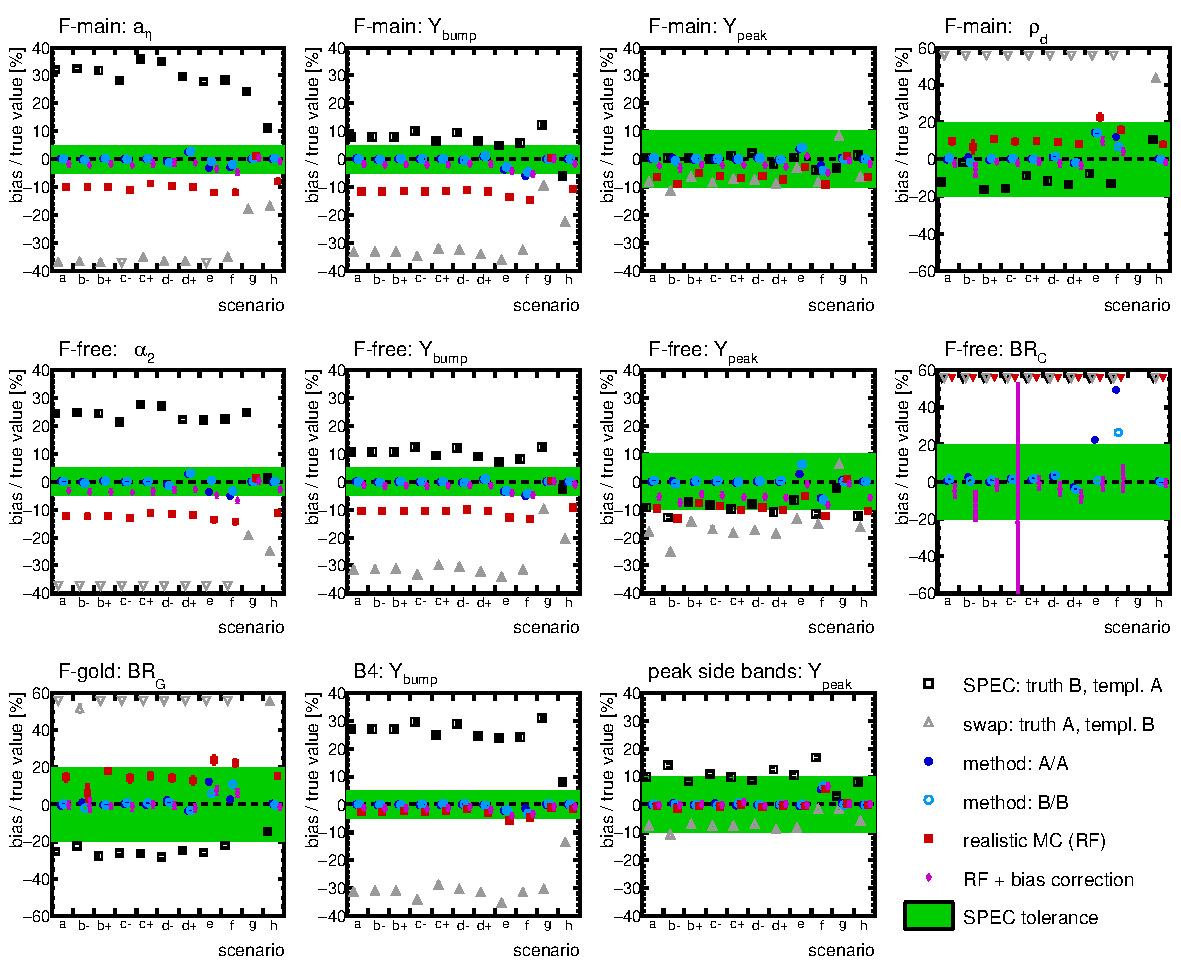
\includegraphics[width=0.92\textwidth]{figs_all/wp4_V1.pdf}
\caption{Spec.\ Fig.~V1: stress closure on simulation, relative bias of every gated quantity in the scenarios (a)--(h).
Selection: no data; pseudo-data built for S0 (PT3 trigger, event vertex in the target region ($\vz>-160$\,mm), \betanew particle identification (pions within $3\sigma$, leptons within $5\sigma$ and with a RICH ring), energy-loss-corrected momenta of all four tracks, all stored combinations of each event (isBest $\ge0$), both pions in the event-vertex fit) at $L=6079.2\,\nbinv$ in cells of the \Mpipi slices $<0.34$, 0.34--0.37, 0.37--0.39, 0.39--0.43, $\ge0.43$\,\GeVcc $\times$ \Mee $<10$, 10--20, $\ge20$\,\MeVcc $\times$ \Mfour 0.400--0.700\,\GeVcc: the data CB rebuilt from Poisson-fluctuated like-sign counts + smoothed SMASH non-$\eta$ background $\times\,c\,(1+bx)$ + raw SMASH $\eta$ classes (SMASH p+p at 4.5\,GeV (standard, lepton and $\eta$ sets, mode A) at its cross sections $\times$ PDG BR $\times$ the $\eta$-decay weights V3, masses moved to the data scale ($M_4'=0.99615\,M_4$, $\Mpipi'=0.9952\,\Mpipi$)). Estimators in the configuration of the specification: F-main, F-free on both \Mee classes, F-gold on \Mee$\ge20$\,\MeVcc; stage A in \Mfour 0.565--0.700\,\GeVcc plus \Mpipi$\ge0.43$\,\GeVcc with \Mfour 0.400--0.5225\,\GeVcc; B4 in the bump window 0.4550--0.5225\,\GeVcc with the background from 0.565--0.700\,\GeVcc; peak side bands with the peak window 0.53364--0.55416\,\GeVcc and side bands 0.5250--0.5336 and 0.5542--0.5628\,\GeVcc; B4 and side bands over all \Mee and \Mpipi. Toys at
$L=6079.2\,\nbinv$ (raw counts, isBest $\ge0$, S0), 500 per point. Truth: smoothed simulated non-$\eta$ background + raw $\eta$ classes + CB
from the data like-sign pairs; toy $N$ and like-sign counts Poisson-fluctuated. Open squares: specification test (truth half B, templates
half A); open triangles: swap; full/open circles: truth and templates from the same half (method); red squares: truth from the full sample,
templates from bootstrap replicas (RF); magenta diamonds: RF with bias correction (RB). Green band: tolerance (5\,\% \aEta, \Ybump; 10\,\%
\Ypeak; 20\,\% \rhod, BR). Scenario g ($\aEta=0$): bias in per cent of the true value of (a). Triangles at the frame: outside the range. Fall-back consequence: estimators that fail are cross-checks only.}
\label{fig:V1}
\end{figure}

\begin{figure}[!tbp]
\centering
\begin{subfigure}{0.49\textwidth}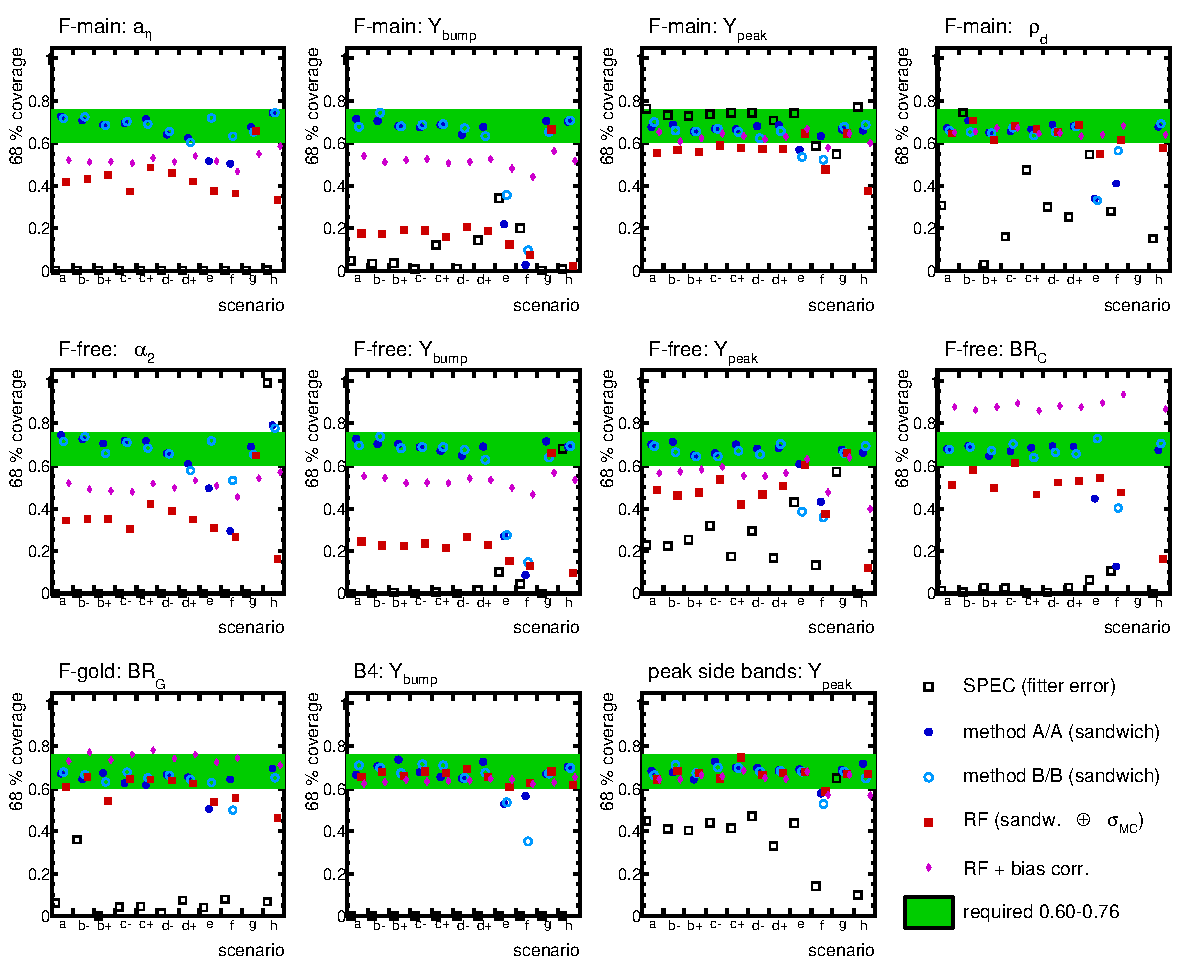
\includegraphics[width=\textwidth]{figs_all/wp4_V1_coverage.pdf}\caption{coverage}\end{subfigure}
\begin{subfigure}{0.49\textwidth}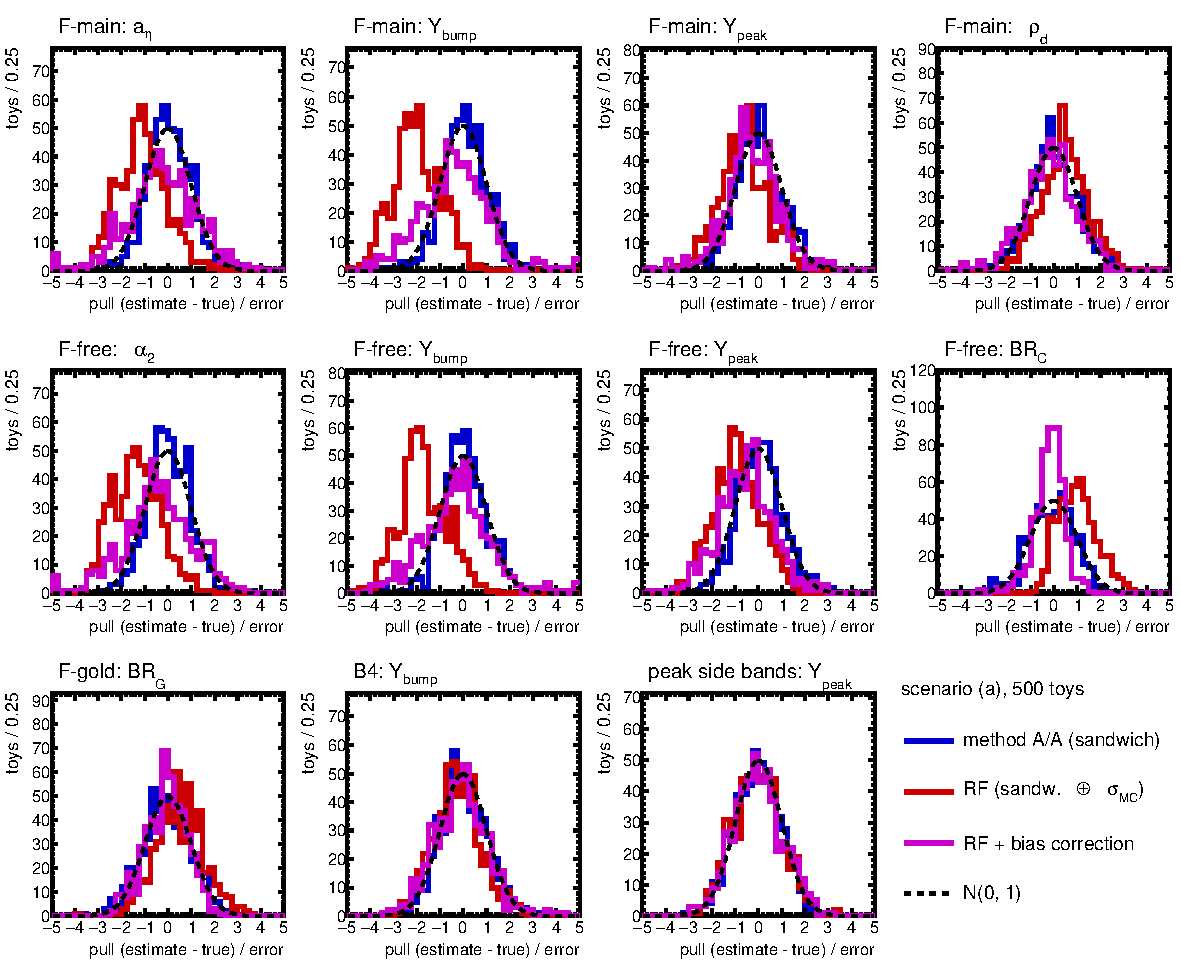
\includegraphics[width=\textwidth]{figs_all/wp4_V1_pulls.pdf}\caption{pulls, scenario (a)}\end{subfigure}
\caption{Selection: no data; the pseudo-data of Fig.~\ref{fig:V1} (built for S0 at $L=6079.2\,\nbinv$ in cells of five \Mpipi slices $\times$ \Mee $<10$, 10--20, $\ge20$\,\MeVcc $\times$ \Mfour 0.400--0.700\,\GeVcc; estimators in the configuration of the specification: template fits on both \Mee classes, stage A in 0.565--0.700\,\GeVcc plus \Mpipi$\ge0.43$\,\GeVcc with \Mfour 0.400--0.5225\,\GeVcc, B4 and peak side bands over all \Mee).
(a) Fraction of toys whose error interval contains the truth: fitter error (specification), sandwich error (method), sandwich
$\oplus\,\sigma_{\mathrm{MC}}$ (realistic); required band 0.60--0.76 (not required in the mis-modelling scenarios e, f). (b) Pull
distributions of scenario (a): method (blue), realistic MC (red), realistic MC with bias correction (magenta); dashed: $N(0,1)$ for 500
toys. Same toys as Fig.~\ref{fig:V1}. Fall-back consequence: estimators that fail are cross-checks only.}
\label{fig:V1cov}
\end{figure}

\textbf{What the toys show.}
\begin{enumerate}\setlength{\itemsep}{0pt}
\item \textbf{Attenuation.} With realistic template noise (RF) every template fit is biased low: \aEta $-10.1$\,\%, \Ybump(F-main)
      $-11.6$\,\%, \Ypeak(F-main) $-6.6$\,\%, \BRG $+14.8$\,\%. The cause is the noise of the \emph{raw signal} templates (C2--C5, \Geta,
      $N_{\mathrm{eff}}$ 10--200 per histogram): a fit that scales a noisy template is pulled towards zero (errors in the regressor).
      BB-lite does not remove it. Splitting the replica effect (\code{wp4_mcsplit.txt}): the raw signal templates make the bias
      (\aEta $-10.2$\,\%), the smoothed background templates make the spread (\aEta rms 9.9\,\%). The side-band estimators do not scale a
      signal template and are not attenuated (B4 $-1.4$\,\%, peak side bands $-0.5$\,\%).
\item \textbf{Simulation-limited.} $\sigma_{\mathrm{MC}}=8.8$\,\% (\aEta), 5.6\,\% (\Ybump), 9.2\,\% (\Ypeak), 9.2\,\% (B4), but 3.7\,\% for
      the peak side bands; $\sigma_{\mathrm{MC}}/\sigma_{\mathrm{stat}}=3.0$ (\aEta), 3.3 (\Ybump), 1.6 (\BRG), 3.6 (B4), 0.42 (peak side bands).
\item \textbf{Errors.} With the sandwich error the method coverage is 0.60--0.74 (F-main), 0.62--0.69 (F-gold), 0.65--0.74 (B4), 0.64--0.73
      (peak side bands); the BB-lite covariance over-covers (0.95) and the data-only Fisher error under-covers (0.56). In RF the F-main
      errors are right (pull width 1.01--1.03) but the bias of $-1.1$ to $-2.0\sigma$ makes the coverage fail (\aEta 0.33--0.49). The bias
      correction (RB) removes the bias (\aEta $-1.7$\,\%, \Ybump $-1.8$\,\%, \BRG $-0.3$\,\%) but inflates the MC error, which the child rms
      then underestimates by a factor of about 1.5 (coverage 0.51--0.59).
\item \textbf{Null scenario} (g): mean pulls 0.01--0.10 (method) and at most 0.23 (RF, RB) for every gated quantity: PASS.
\item \textbf{Expected $\chi^2$ from template noise alone} (perfect physics model, full-sample templates): F-main 2.83, stage A 2.10 in
      scenario (a); 6.1 and 2.5 for $\aEta=1$. A data $\chi^2$/ndf of 2--3 is therefore not by itself evidence of mis-modelling.
\item \textbf{Mis-modelling scenarios} (method configurations; inputs of families S3, S6): (e) $\omega$: F-main \Ybump $-3.7$/$-2.7$\,\%,
      \Ypeak $+3.6$/$+4.1$\,\%, \rhod $+14$\,\%, B4 $-2.3$/$-2.0$\,\%, peak side bands $-0.4$/$-0.1$\,\%; (f) mass transfer: F-main \Ybump
      $-6.0$/$-4.7$\,\%, B4 $-1.6$/$-3.3$\,\%, peak side bands $+5.5$/$+6.5$\,\%, \BRG $+2.7$/$+11.0$\,\%.
\item \textbf{Correlations}: corr$(\rhod,\kappa)$ 0.26 mean, 0.60 at most (fall-back limit 0.9); corr$(\aEta,b)$ 0.15--0.35 (limit 0.7).
\item Scenario (i), true CB like the per-cell geometric mean: \aEta $+4.1$/$+4.8$\,\% (method), $-7.8$\,\% (RF); \Ybump $+1.6$/$+1.8$\,\%;
      B4 $+0.5$/$+1.5$\,\%; peak side bands $+0.1$/$-1.5$\,\% (family S1).
\end{enumerate}

\begin{table}[H]
\centering
\caption{Verdict of the closure test per estimator (WP4, \code{verdict.txt}). The adopted decision rule (WP4, a deviation from the
specification, D22, approved by the analyst) uses the method configurations and RF; ``with bias correction'' uses RB instead of RF. The BA column is the specification's
configuration, reported but not used as the gate. Fall-back consequence: estimators that fail are cross-checks only.}
\label{tab:verdict}
\small
\resizebox{\textwidth}{!}{%
\begin{tabular}{@{}l l l l l l@{}}
\toprule
estimator & BA (spec.\ configuration, not the gate) & method (AA, BB) & realistic (RF) & RF + bias corr.\ (RB) & decision (adopted rule) \\
\midrule
F-main & FAIL & FAIL ((f) \Ybump $-6.0$\,\%) & FAIL (\aEta $-10$\,\%) & FAIL (coverage) & \textbf{FAIL} \\
F-free & FAIL & FAIL (\BRC in e, f) & FAIL & FAIL & \textbf{FAIL} \\
F-gold (\BRG) & FAIL & PASS & FAIL ((e) $+23.9$\,\%) & FAIL marginal & \textbf{FAIL} \\
B4 (\Ybump) & FAIL & PASS & FAIL marginal ((e) $-5.8$\,\%) & PASS & \textbf{FAIL marginal} \\
peak side bands (\Ypeak) & FAIL & PASS & PASS & FAIL marginal (h: 0.57) & \textbf{PASS} \\
X17 & \multicolumn{5}{l}{validated separately (\S\ref{sec:x17val})} \\
\bottomrule
\end{tabular}}
\end{table}

\textbf{Family-S10 entries} ($|$bias$|$ of scenario (a) in RF, the estimators as specified): peak side bands 0.5\,\%; B4 2.6\,\%; F-main
\aEta 10.1\,\%, \Ybump 11.6\,\%, \Ypeak 6.6\,\%, \rhod 9.7\,\%; \BRG 14.8\,\%. With the bias correction they would be 0.2, 1.3, 1.7, 1.8, 2.4,
2.5 and 0.3\,\%. The BA values ($+32$\,\% etc.) are template-half noise and are not used.

\textbf{Implementation choices carried into the data analysis}, so that the verdict applies to the data numbers: one-scale smoothing
likelihood (per-bin scales biased the normalisation low by 10--40\,\%); parent shapes for sparse histograms ($N_{\mathrm{eff}}<20$); the
$\eta$ content of the upper region subtracted before the B4 extrapolation; the unweighted C4+C5 leakage for the side bands; \kB and
$a\kappa$(C3+C4) fixed from F-main in F-gold; \Geta$\times\alpha_2 g$ in F-free and F-gold; sandwich errors. The toys have no event-group
clustering (the data event-group error is about 1\,\% larger in P) and per-cell Poisson CB fluctuations (pull widths 0.94--1.06 show this is
harmless). X17 was validated separately (\S\ref{sec:x17val}).

%======================================================================
\section{Extraction with template fits (stage B, cross-checks)}
\label{sec:fit}
%======================================================================
\inshort{the template fits give $\aEta=0.382\pm0.017\,(\mathrm{stat})\pm0.040\,(\mathrm{MC})$ of SMASH (F-main), close to the side-band result, with $\chi^2_{\mathrm{GLS}}/\mathrm{ndf}=2.59$. They failed the closure test, so every number of this section is a cross-check; the fits still provide inputs (the other $\eta$ terms, background shapes, the variants of the systematics).}
\notebox{\textbf{Every number of this section is a CROSS-CHECK}: F-main, F-free and F-gold failed the closure test (\S\ref{sec:val}).
They provide the ``other $\eta$'' terms of the side-band estimators (\S\ref{sec:sb}), the \aEta prior and the background shapes of the
X17 fit, the refits of the systematic variants and the ratios of \S\ref{sec:phys}. All numbers were reproduced by an independent
verifier (v5) with its own code and a different minimiser: \aEta $0.382284$ vs $0.382283$, yields and ratios to $10^{-5}$.}

\subsection{Procedure}
\begin{enumerate}\setlength{\itemsep}{0pt}
\item \textbf{Covariance of the data.} One event can give several counts, so neighbouring cells are correlated. For every data sample used
      (S0 all, folds, periods, isBest $=1$, ``pre''; F10 and F5g) the products of the counts of one event group in every pair of cells
      are summed. The variance of the F10 total is $1.19\,N$ (S0), $1.26\,N$ (``pre''), $1.00\,N$ for isBest $=1$ (one count per event).
\item \textbf{Templates.} S0 nominal simulation in expected raw counts; $G_D$, $G_C$ smoothed exactly as in WP4 (one common scale per
      histogram, F5g $G_C$ of S2--S4 with the shape of its F10 parent); C2--C5 and \Geta raw with BB-lite; 100 replicas, smoothing redone.
\item \textbf{Fitter.} The WP4 estimator in general form (Poisson fixed point by Fisher scoring, variance $\max(\mu,1)+k^2\mathrm{var(CB)}+$
      BB-lite); on the configuration validated by WP4 it agrees with the WP4 code to all printed digits.
\item \textbf{Errors.} stat $=$ sandwich with three parts: the event-group covariance of $N$, the full $700\times700$ CB covariance from the
      200 like-sign replicas, and one part for each Gaussian constraint; MC $=$ spread of 100 refits with one simulation replica each;
      total $=$ stat $\oplus$ MC. The replica mean minus the nominal value is the attenuation shift of WP4; ``bias-corrected'' $=2v-$mean
      is given as information only (its coverage failed in WP4).
\end{enumerate}

\subsection{The E1 fall-back and the nominal fit}
\label{sec:fmain}
F-main as specified (E1 + E2, \kEone free) gives $\kEone=7.63\pm0.52\,(\mathrm{stat})\pm1.64\,(\mathrm{MC})$, outside 0.8--3 as in stage A.
The fall-back ``drop E1, $\kappa=1\pm0.2$'' fired: the \textbf{nominal F-main uses F10 E2 only} (350 bins) with a free \aEta, \rhod,
$c_1\dots c_5$, $b$, \kB and constraints $\kappa=1\pm0.2$, $g=1\pm0.3$, $\kEtwo=1\pm0.05$, and the background model M1 frozen in stage A.

\begin{table}[H]
\centering
\caption{Spec.\ Table~E1: parameters of F-main (CROSS-CHECK: it failed the closure test), value $\pm$ stat $\pm$ MC; $^{c}$ constrained. Columns:
nominal (E2, $\kappa=1\pm0.2$), as specified (E1+E2, \kEone free), ``pre'' (E2), data isBest $=1$ (E2, with the isBest $\ge0$
templates). S0 unless stated, $L=6079.2\,\nbinv$. Largest correlations of the nominal fit (stat + MC): $c_j$--$c_k$ about 0.97, $c_j$--\kB
about $-0.9$, \aEta--$g$ $-0.53$, \aEta--$\kappa$ $-0.44$, \aEta--$c_j$ $-0.37$ to $-0.41$, \aEta--$b$ 0.05, \rhod--$\kappa$ 0.04. Source:
WP5 (\code{wp5_tableE1.txt}), verified by v5. Fall-backs: E1 dropped ($\kappa=1\pm0.2$); template fits demoted to cross-checks.}
\label{tab:E1}
\footnotesize
\resizebox{\textwidth}{!}{\tabin{wp5_tableE1.tex}}
\end{table}

\textbf{Fit quality.} Pearson $\chi^2=1158/341=3.40$; GLS with the replica covariance $883.7/341=2.59$ at the fit (2.16 minimised); WP4
expects about 2.8 from template noise alone. The verifier v5 showed that the GLS value is not converged in the number of replicas (the
replica covariance has rank 99 for 350 bins); with the exact diagonal variance of the raw signal templates plus the replica covariance of the
smoothed background (a ``hybrid'' GLS) the value is $648/341=1.90$ at the fit (1.67 minimised). The criterion $\chi^2/\mathrm{ndf}\le1.2$
fails either way, and the specified error scale $\sqrt{\chi^2/\mathrm{ndf}}$ is 1.61 (GLS) or 1.38 (hybrid GLS); it is given as a separate
column and not applied in the tables. The misfit sits in 0.400--0.455 (Pearson 406 for 55 bins; S2 122, S3 216), in CR-U (420 for 125
bins), in B (181 for 70 bins, S5 alone 89) and in 0.5225--0.565 (125 for 85 bins).

\begin{figure}[H]
\centering
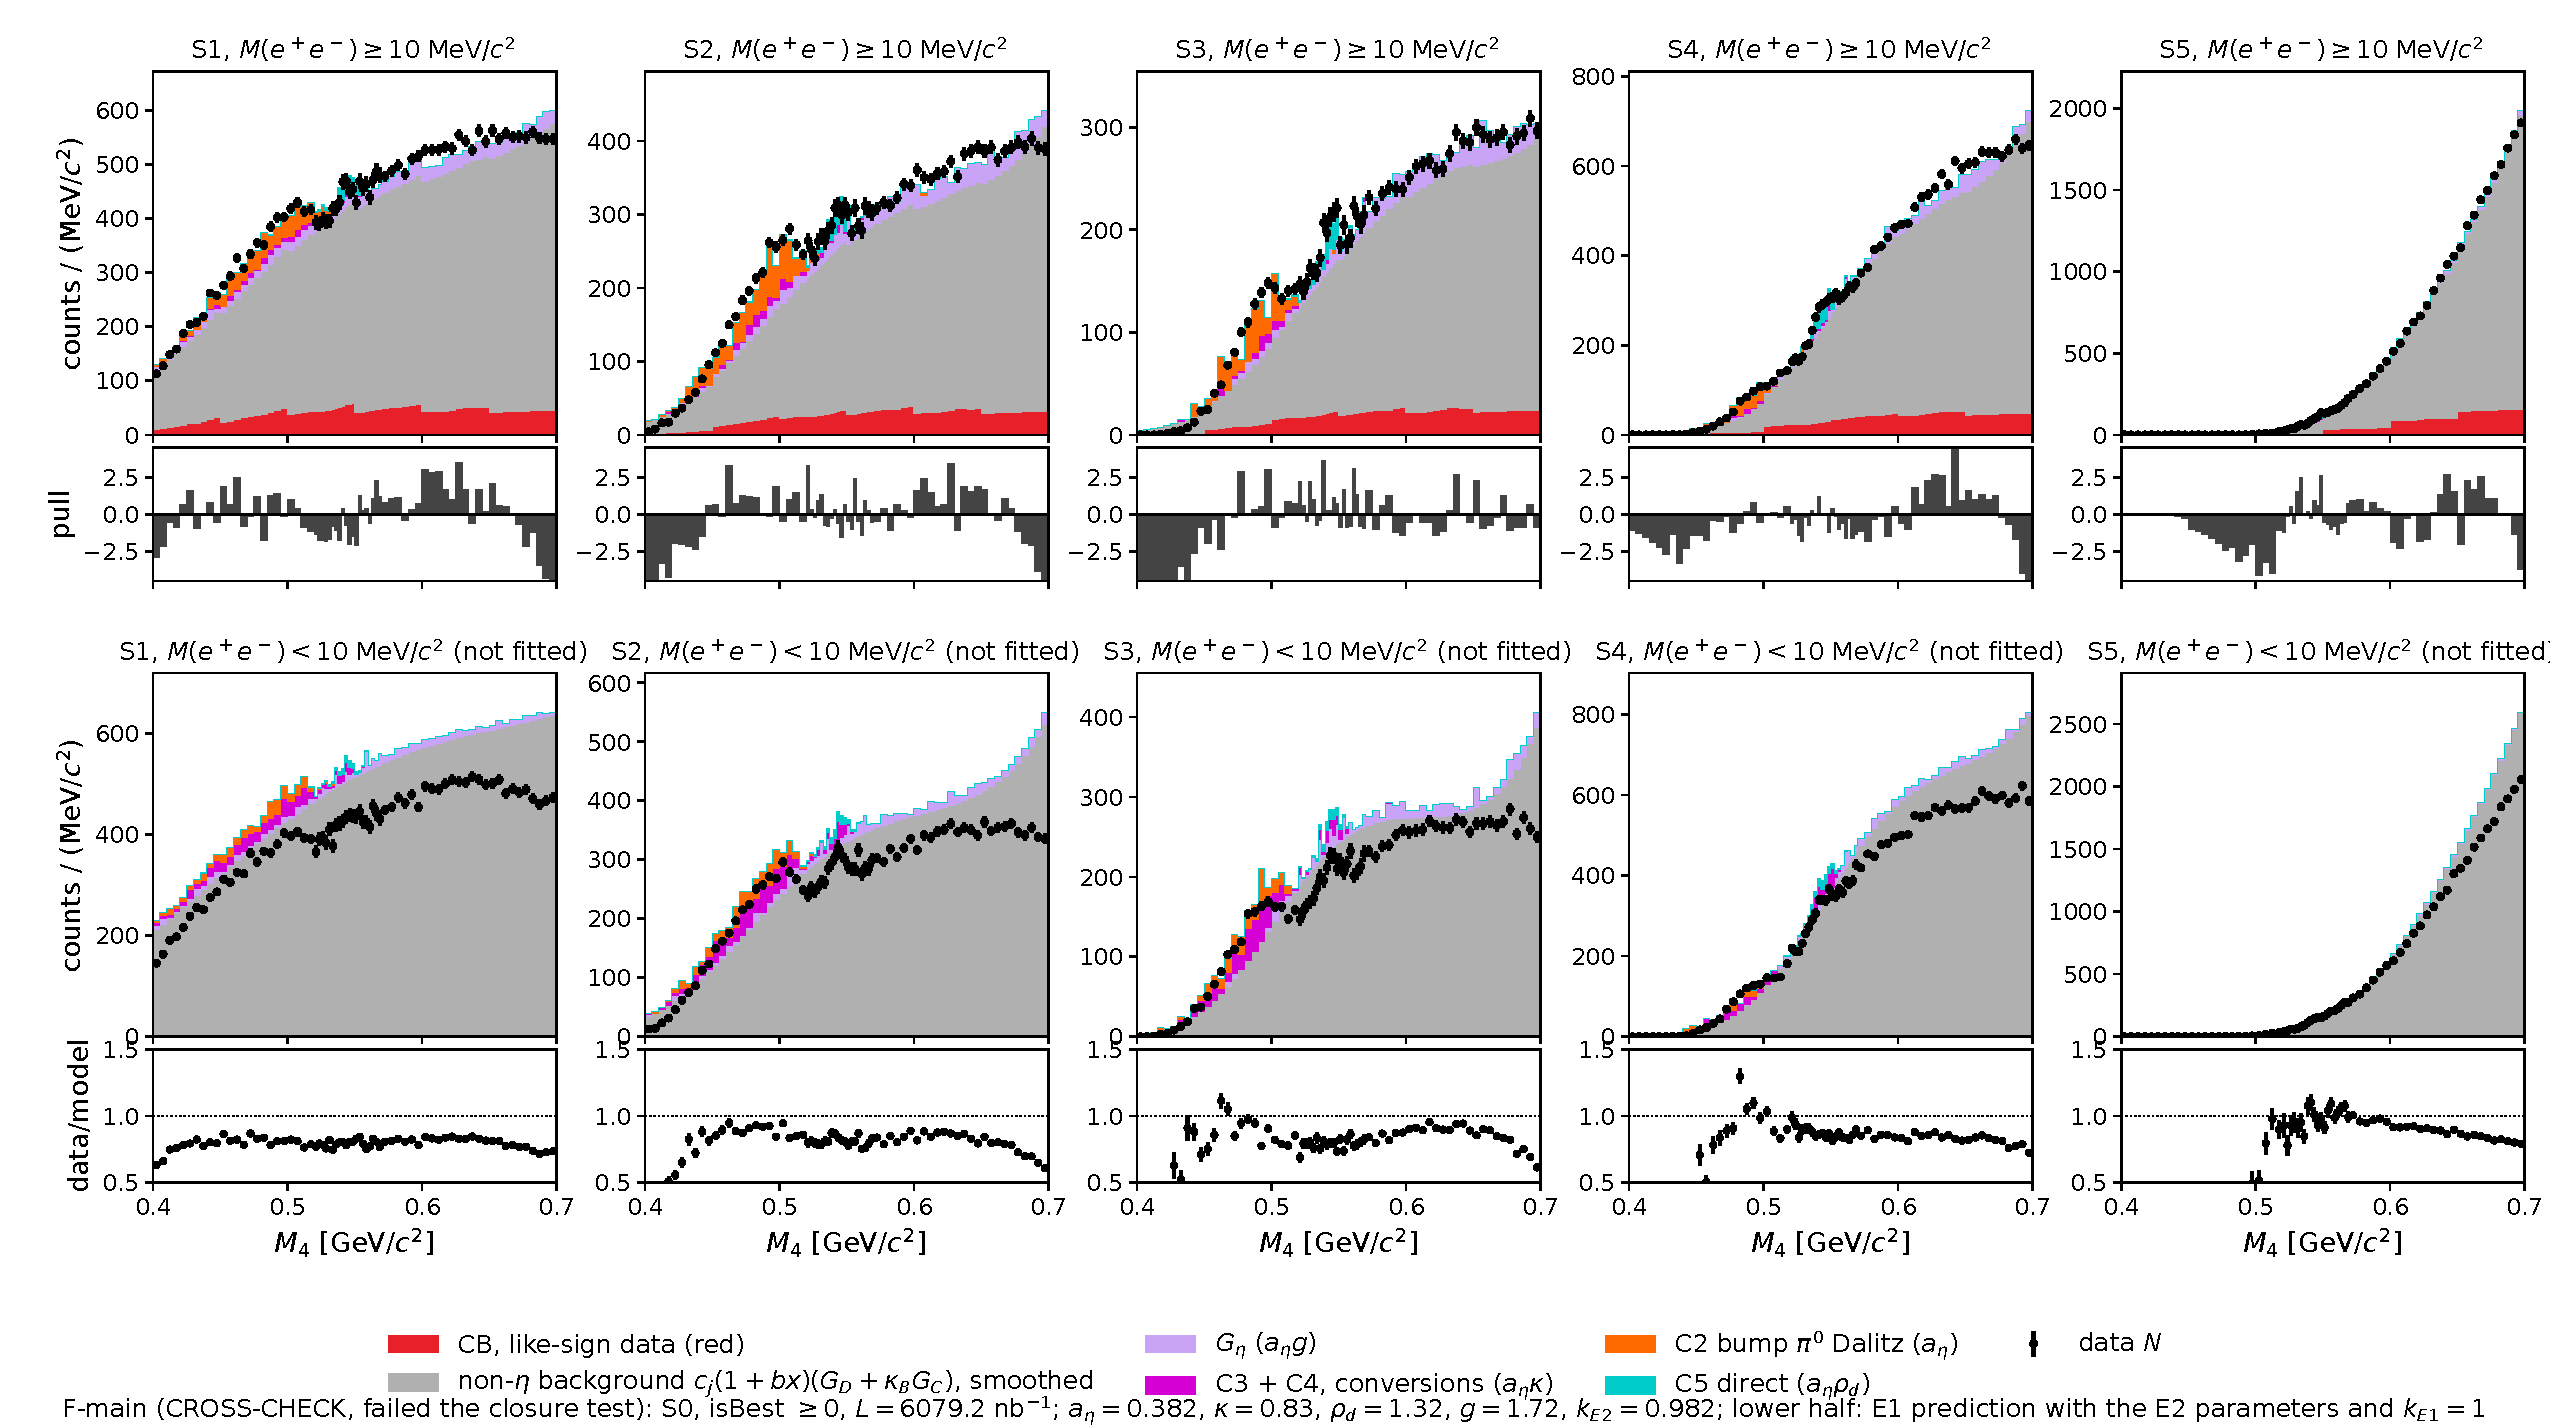
\includegraphics[width=\textwidth]{figs_all/fix_E1_cnt.pdf}
\caption{Spec.\ Fig.~E1: stage-B fit F-main (CROSS-CHECK, failed the closure test).
Selection: data, S0 (PT3 trigger, event vertex in the target region ($\vz>-160$\,mm), \betanew particle identification (pions within $3\sigma$, leptons within $5\sigma$ and with a RICH ring), energy-loss-corrected momenta of all four tracks, all stored combinations of each event (isBest $\ge0$), both pions in the event-vertex fit); \Mfour 0.400--0.700\,\GeVcc (5\,\MeVcc bins, 2.5\,\MeVcc in 0.520--0.570); columns: the \Mpipi slices $<0.34$, 0.34--0.37, 0.37--0.39, 0.39--0.43, $\ge0.43$\,\GeVcc; upper half \Mee$\ge10$\,\MeVcc (fitted), lower half \Mee$<10$\,\MeVcc (not fitted); CB $=2\sqrt{N_{++}N_{--}}$ of the like-sign data with the same cuts (10\,\MeVcc cells of \Mfour, $k=1$), shared out by the like-sign share of each 50\,\MeVcc band; SMASH p+p at 4.5\,GeV (standard, lepton and $\eta$ sets, mode A) at its cross sections $\times$ PDG BR $\times$ the $\eta$-decay weights V3, masses moved to the data scale ($M_4'=0.99615\,M_4$, $\Mpipi'=0.9952\,\Mpipi$), same cuts, non-$\eta$ templates smoothed (exponential of a cubic polynomial). Data S0, isBest $\ge0$, $L=6079.2\,\nbinv$, counts per \MeVcc.
Columns: slices S1--S5. Upper half: \Mee$\ge10$\,\MeVcc, the fitted class, with pulls $(N-\mu)/\sigma$ ($\sigma^2$: event-group variance of
$N$ scaled to the model + $k^2$var(CB) + template variance). Lower half: \Mee$<10$\,\MeVcc, \emph{not} fitted (fall-back ``drop E1''):
prediction with the E2 parameters and $\kEone=1$, and data/model (the data are 0.75--0.90 of the prediction). Black: data $N$. Stacked, in the
common colours: CB (red), smoothed non-$\eta$ simulation $c_j(1+bx)(G_D+\kB G_C)$ (grey), \Geta (violet), C3+C4 (magenta), C2 (orange),
C5 (cyan), at SMASH $\sigma_{\mathrm{prod}}\times$PDG BR$\times$V3 times the fitted amplitudes. Redrawn with the fit of the verifier's
library (\code{fix_E1.py}; same parameters to $10^{-5}$) with the legend outside the data. Fall-backs: E1 dropped, template fits demoted. The
fit as specified (E1+E2, $\kEone=7.6$) is in Fig.~\ref{fig:E1spec}.}
\label{fig:E1}
\end{figure}

\begin{figure}[H]
\centering
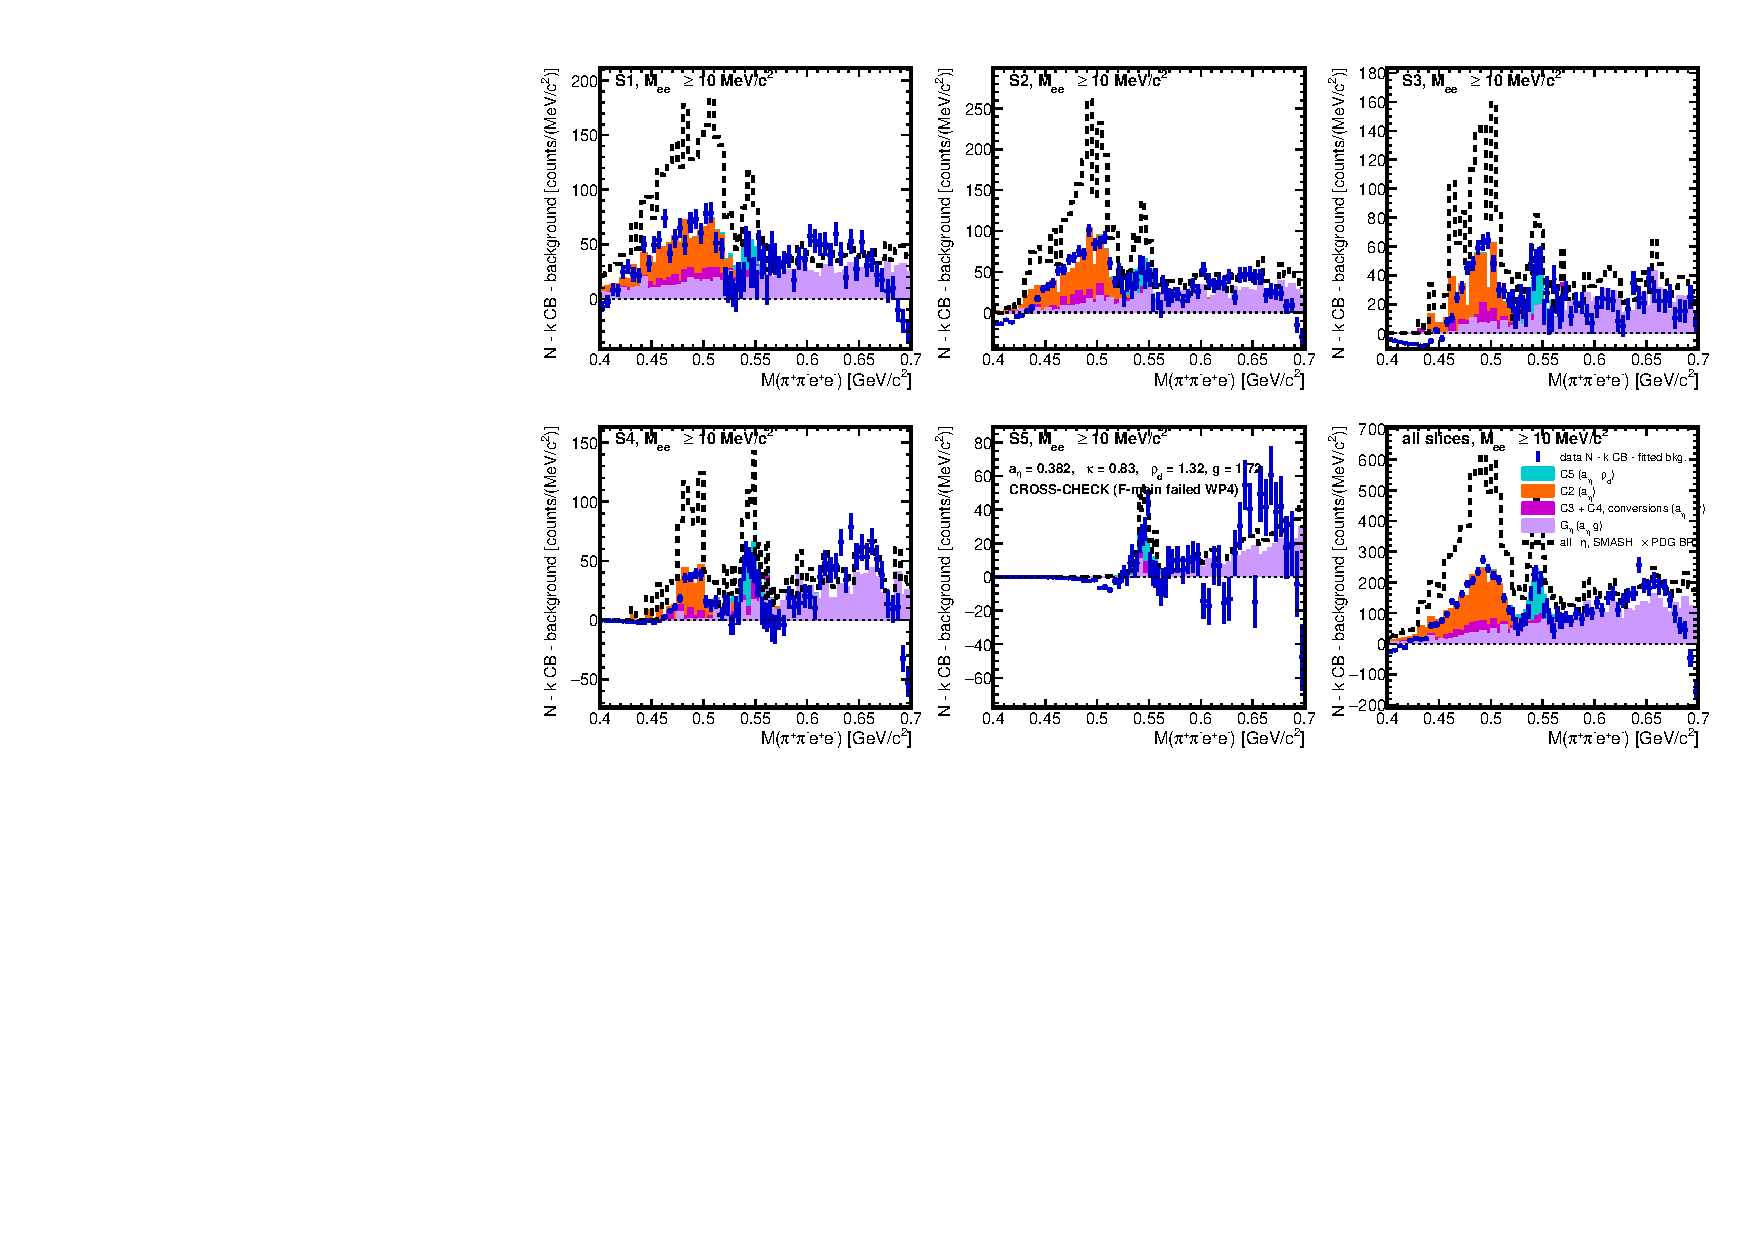
\includegraphics[width=0.95\textwidth]{figs_all/fix_E2_cnt.pdf}
\caption{Spec.\ Fig.~E2: data minus the measured CB minus the fitted non-$\eta$ background, per slice, \Mee$\ge10$\,\MeVcc (blue); errors:
event-group variance of $N$ + CB variance.
Selection: data, S0 (PT3 trigger, event vertex in the target region ($\vz>-160$\,mm), \betanew particle identification (pions within $3\sigma$, leptons within $5\sigma$ and with a RICH ring), energy-loss-corrected momenta of all four tracks, all stored combinations of each event (isBest $\ge0$), both pions in the event-vertex fit); \Mee$\ge10$\,\MeVcc; \Mfour 0.400--0.700\,\GeVcc (5\,\MeVcc bins, 2.5\,\MeVcc in 0.520--0.570); one panel per slice (the \Mpipi slices $<0.34$, 0.34--0.37, 0.37--0.39, 0.39--0.43, $\ge0.43$\,\GeVcc) and their sum; CB $=2\sqrt{N_{++}N_{--}}$ of the like-sign data with the same cuts (10\,\MeVcc cells of \Mfour, $k=1$), shared out by the like-sign share of each 50\,\MeVcc band; background and $\eta$ classes of the F-main fit with SMASH p+p at 4.5\,GeV (standard, lepton and $\eta$ sets, mode A) at its cross sections $\times$ PDG BR $\times$ the $\eta$-decay weights V3, masses moved to the data scale ($M_4'=0.99615\,M_4$, $\Mpipi'=0.9952\,\Mpipi$), same cuts. Stacked, in the common colours: the fitted $\eta$ classes C2$\times\aEta$ (orange),
C3+C4$\times\aEta\kappa$ (magenta, conversions), C5$\times\aEta\rhod$ (cyan), \Geta$\times\aEta g$ (violet). Dotted: all $\eta$ classes at SMASH $\times$ PDG BR ($a=\kappa=\rho=g=1$); its spikes are single heavy simulated
entries. Last panel: sum of the slices. S0, isBest $\ge0$, $L=6079.2\,\nbinv$. CROSS-CHECK (fall-backs: E1 dropped, template fits demoted).
Version of the verifier v5 (\code{v5_figE2.C}; its legend no longer hides the S5 data, where the residuals are negative, about $-5$ to
$-8$ counts/\MeVcc in 0.48--0.53), recoloured (\code{fix_figE2.C}).}
\label{fig:E2}
\end{figure}

\subsection{Yields, ratios and the class scales}
\label{sec:ffree}
\begin{table}[H]
\centering
\caption{Spec.\ Table~E2: yields (raw counts $\times64/63$, not efficiency corrected) and ratios of the template fits (CROSS-CHECK). Error columns:
stat (event groups), CB (replicas + \kEtwo), nuisance ($g$, $\kappa$), MC; S10 $=$ WP4 RF bias of scenario (a); last column: bias-corrected
value (information). S0, isBest $\ge0$, $L=6079.2\,\nbinv$. Source: WP5 (\code{wp5_tableE2.txt}), verified by v5. Fall-backs: E1 dropped ($\kappa=1\pm0.2$); template fits demoted to cross-checks.}
\label{tab:E2}
\small
\resizebox{\textwidth}{!}{\tabin{fix_tE2.tex}}
\end{table}

\begin{itemize}\setlength{\itemsep}{0pt}
\item \textbf{Yields}: $\Ybump=19\,426$ ($\pm687$ stat $\pm196$ CB $\pm677$ nuis.\ $\pm2274$ MC), $\Ypeak=5045$ ($\pm298\pm86\pm181\pm720$);
      visible yields $Y/L$ bump $3.20\pm0.16\pm0.37$, peak $0.83\pm0.06\pm0.12$ visible counts per \nbinv. Replica shifts (attenuation): \aEta $-0.050$
      ($-13$\,\%), \Ybump $-16$\,\%, \Ypeak $-14$\,\%; MC/stat $=2.3$ (\aEta), 2.3 (\Ybump), 2.0 (\Ypeak).
\item \textbf{F-gold} (F5g, \Mee$\ge20$\,\MeVcc; $\alpha_2$, $\alpha_5$, $g$, $c_j$, $b$, \kEtwo free; \kB and $a\kappa$(C3+C4) from F-main):
      $\alpha_2=0.388\pm0.019\pm0.046$ (the same as \aEta), $\alpha_5=0.385\pm0.054\pm0.072$, $g=2.19\pm0.18\pm0.33$, $\chi^2$ 902/342;
      $\BRG=2.68\times10^{-4}\,\alpha_5/\alpha_2=(2.65\pm0.34\pm0.13\pm0.05\pm0.70)\times10^{-4}$ (stat, CB, nuisance, MC; $-0.0\sigma$ from PDG 2020
      $2.68\pm0.11$; bias-corrected 2.53). With the PDG 2026 rescaling of the simulated classes (\S\ref{sec:p2}) $\BRG=2.67\times10^{-4}$, compared
      with PDG 2026 $2.76\pm0.16$. The MC error is 0.70 here (F-gold refitted per replica with the nominal F-main inputs) and 0.66 in
      Tables~\ref{tab:S1} and \ref{tab:P2} (WP7: the whole chain F-main $\to$ F-gold refitted per replica).
\item \textbf{\rhod}: $\BRA=2.68\times10^{-4}\,\rhod=(3.52\pm0.29\pm0.09\pm0.04\pm0.61)\times10^{-4}$, $+1.2\sigma$ from PDG 2020 with these errors
      ($+0.26\sigma$ with the systematic of Table~\ref{tab:S1}); 3.54 with the PDG 2026 rescaling.
\item \textbf{F-free} (free $\alpha_2\dots\alpha_5$): on E2 alone the conversion classes are not determined ($\alpha_3=-0.07\pm0.24$,
      $\alpha_4=0.29\pm0.19$, $R_{34}=-4.2\pm4.8$ total), so \textbf{\BRC is withdrawn}. On E1+E2 (a labelled cross-check, E1 being the class
      whose model failed) $R_{34}=0.92\pm0.18\,(\mathrm{stat})\pm0.24\,(\mathrm{MC})$ (total 0.30, Table~\ref{tab:E2}), consistent with 1, and
      $\BRC=(3.6\pm0.9\pm3.6)\times10^{-4}$.
\item \textbf{$\kappa$ and \kB}: nominal $\kappa=0.83\pm0.30$, dominated by its constraint (0.13 of the 0.145 stat error); \kB $=1.95\pm0.93$
      (MC-dominated). With $\kappa$ free, $\kappa=0.33\pm0.52$ and \aEta rises by 11\,\%. E1+E2: $\kappa=0.50\pm0.16$, $\kB=1.11\pm0.05$, but E1
      holds an unmodelled component (\kEone$=7.6$). The E1 data are 0.75--0.90 of the prediction from the E2 parameters (lower half of
      Fig.~\ref{fig:E1}). F-main alone gives no data-driven conversion scale; the per-class side bands and the X17 fit (\S\ref{sec:p2}) do,
      and they point to $\kappa\approx0.4$--0.5.
\item \textbf{$g$} is pulled to $1.72\pm0.40$, 2.4$\sigma$ of its prior above 1 (2.2 in F-gold and E1+E2, 2.56 when free): \Geta is the
      largest $\eta$-related term in E2 above 0.56\,\GeVcc. The effective \Geta scale used by the side bands is $\aEta g=0.66$.
\end{itemize}

\subsection{Variants and the dependence on the estimator}
\begin{table}[H]
\centering
\caption{F-main variants (change relative to the nominal; GLS $\chi^2$ at the fit, 341 degrees of freedom unless stated). Source: WP5
(\code{wp5_acceptance.txt}). Fall-backs: E1 dropped ($\kappa=1\pm0.2$); template fits demoted to cross-checks.}
\label{tab:fitvar}
\small
\begin{tabular}{@{}l r r r r@{}}
\toprule
variant & GLS $\chi^2$ & \aEta & \Ybump & \Ypeak \\
\midrule
nominal & 883.7 & 0.382 & 19\,426 & 5\,045 \\
$b$ constrained to stage A ($-0.068\pm0.025$) & 888.3 & $-0.8$\,\% & $-0.8$\,\% & $-0.8$\,\% \\
+ quadratic term (S3) & 796.7 & $\mathbf{+39}$\,\% & $+32$\,\% & $+5$\,\% \\
per-slice tilts (S3) & 901.8 & $-2.7$\,\% & $-2.9$\,\% & $+1.3$\,\% \\
$\kappa$ free & 895.7 & $+11.5$\,\% & $-14.2$\,\% & $-12.9$\,\% \\
$g$ free, $g=2.56$ (S8) & 947.1 & $-6.1$\,\% & $-1.8$\,\% & $+2.3$\,\% \\
range 0.42--0.70 (S5) & 734.3/321 & $-7.8$\,\% & $-5.4$\,\% & $-8.2$\,\% \\
range 0.45--0.70 (S5) & 541.6/291 & $-5.0$\,\% & $-2.5$\,\% & $-11.1$\,\% \\
raw non-$\eta$ templates (S4) & 3389 & $+30$\,\% & $-16$\,\% & $+28$\,\% \\
exp(pol2) smoothing (S4) & 2019 & $+39$\,\% & $+50$\,\% & $+95$\,\% \\
\bottomrule
\end{tabular}
\end{table}

The raw and exp(pol2) variants are rejected by their $\chi^2$. The quadratic term is not: its minimised GLS $\chi^2$ equals the nominal one
(738.3 vs 737.5), yet it moves \aEta from 0.38 to 0.53. \textbf{The bump amplitude is degenerate with the curvature of the background}; the
full-fit tilt ($b=-0.011\pm0.021$) and the stage-A tilt ($-0.068\pm0.025$) differ by 1.7$\sigma$. This confirms the ``extrapolated''
label of the bump.

The verifier v5 fitted the same histograms with other estimators:

\begin{table}[H]
\centering
\caption{Dependence on the estimator (same histograms; verifier v5, \code{tables_all/v5_verification.txt}). Fall-backs: E1 dropped ($\kappa=1\pm0.2$); template fits demoted to cross-checks.}
\label{tab:estdep}
\small
\begin{tabular}{@{}p{8.6cm} r r r r@{}}
\toprule
estimator & \aEta & \Ybump & \Ypeak & \BRG [$10^{-4}$] \\
\midrule
WP5 fixed point (reference) & 0.3823 & 19\,426 & 5\,045 & 2.65 \\
Poisson likelihood with a Barlow--Beeston-lite nuisance per bin (textbook D12) & 0.3813 & $-1.1$\,\% & $-0.4$\,\% & 2.69 \\
plain Poisson likelihood without template variance & 0.3349 & $-5$\,\% & $-4$\,\% & 2.32 \\
GLS with the replica covariance, minimised & 0.485 & 24\,228 & 5\,541 & \\
hybrid GLS, minimised & 0.513 & 26\,335 & 6\,193 & \\
\bottomrule
\end{tabular}
\end{table}

In both GLS fits \rhod falls to 1.07--1.12 and $g$ from 1.72 to 0.47--0.50; with the hybrid GLS the quadratic term is no longer needed
($\Delta\chi^2=1.2$). Once the correlated noise of the smoothed background may absorb shape, the split bump / \Geta / background changes by
2.5--3 $\sigma_{\mathrm{MC}}$. \textbf{The F-main \aEta, \Ybump and $g$ are model- and estimator-limited at the 25--35\,\% level}; the
replica MC error (10\,\%) does not cover this, and family S4 carries the hybrid-GLS variant (\S\ref{sec:syst}).

\subsection{Consistency tests and the mass scale}
\label{sec:cons}
\begin{itemize}\setlength{\itemsep}{0pt}
\item \textbf{Per slice}: \aEta $=0.356$, 0.394, 0.406, 0.353, 0.506 (stat 0.030, 0.020, 0.024, 0.027, 0.076); $p=0.92$ with stat + MC,
      0.11 with stat only, 0.94 for S1--S4. The fall-back ``per-slice $p<0.01$'' did not fire.
\item \textbf{Folds}: \aEta $0.356\pm0.020$ / $0.395\pm0.020$ ($z=-1.37$ with these errors; WP5 had quoted $-1.69$); \Ybump $z=-1.22$, \Ypeak
      $z=-1.55$, DR$_F$ $z=-0.91$ (WP7, \code{wp7_tests.txt}); joint test of all free parameters $\chi^2=10.8/12$, $p=0.55$.
\item \textbf{``pre''}: \aEta $0.383\pm0.018\pm0.040$, \rhod 1.36, DR $1.20\pm0.07\pm0.15$; \kEtwo $=0.68\pm0.03$ (the spread rule overestimates
      the CB of ``pre''); GLS $\chi^2$/ndf 3.86.
\item \textbf{isBest $=1$} (ratio to isBest $\ge0$, same templates): \aEta $0.867\pm0.055$, \Ybump $0.868\pm0.063$, \Ypeak $0.888\pm0.090$,
      DR $1.023\pm0.081$ (stat errors are an independent-sample upper bound; MC 0.010--0.019).
\item \textbf{Periods} (background shape, $\kappa$, $g$ fixed; templates $\times$ the luminosity share): \aEta $0.367\pm0.012$ (I),
      $0.423\pm0.031$ (IIA), $0.383\pm0.019$ (IIB), $0.368\pm0.015$ (III), $\chi^2=3.2/3$ ($p=0.36$); DR 1.29, 0.68, 1.02, 1.21, $p=0.038$. The
      stability test with the normalisation factors is in \S\ref{sec:periods}.
\end{itemize}

\label{sec:mscale}
\textbf{Mass scale.} Refits with the factory templates at $s=0.99521$, 0.99525, 0.99615, 0.99705 (fixed-weight $\chi^2$, whose minimum is the
fit's fixed point): whole fit $\hat s=0.99653\pm0.00019$ ($+1.95\sigma$ from 0.99615); peak region 0.5225--0.565 alone $\hat s=0.99500\pm0.00057$
($-2.01\sigma$, 0.6\,\MeVcc at the peak). The two pull in opposite directions, both within the family-S6 variation $\pm0.0009$. The verifier
v5 notes that the peak-region minimum is not bracketed (it lies below the lowest template, and $\chi^2(0.99521)$ is 0.09 above
$\chi^2(0.99525)$): \flag{WP5 ``PASS'' (with the $\chi^2$-scaled error, $-1.79\sigma$) is read here as MARGINAL / not demonstrated.}
\textbf{Resolution}: in the whole fit $r_{\mathrm{res}}=1.10$ is preferred over $r_{\mathrm{res}}=1$ by a fixed-weight $\Delta\chi^2=31$, but in the peak region alone
$r_{\mathrm{res}}=0.89$ and 1.10 lower $\chi^2$ by only 2.9 and 1.8: no significant preference there; the whole-fit preference comes from outside the
peak and is opposite to D8, where the data peak (5.44\,\MeVcc) is narrower than the simulated one (6.09\,\MeVcc) (v5 correction of the WP5
text).

\begin{figure}[H]
\centering
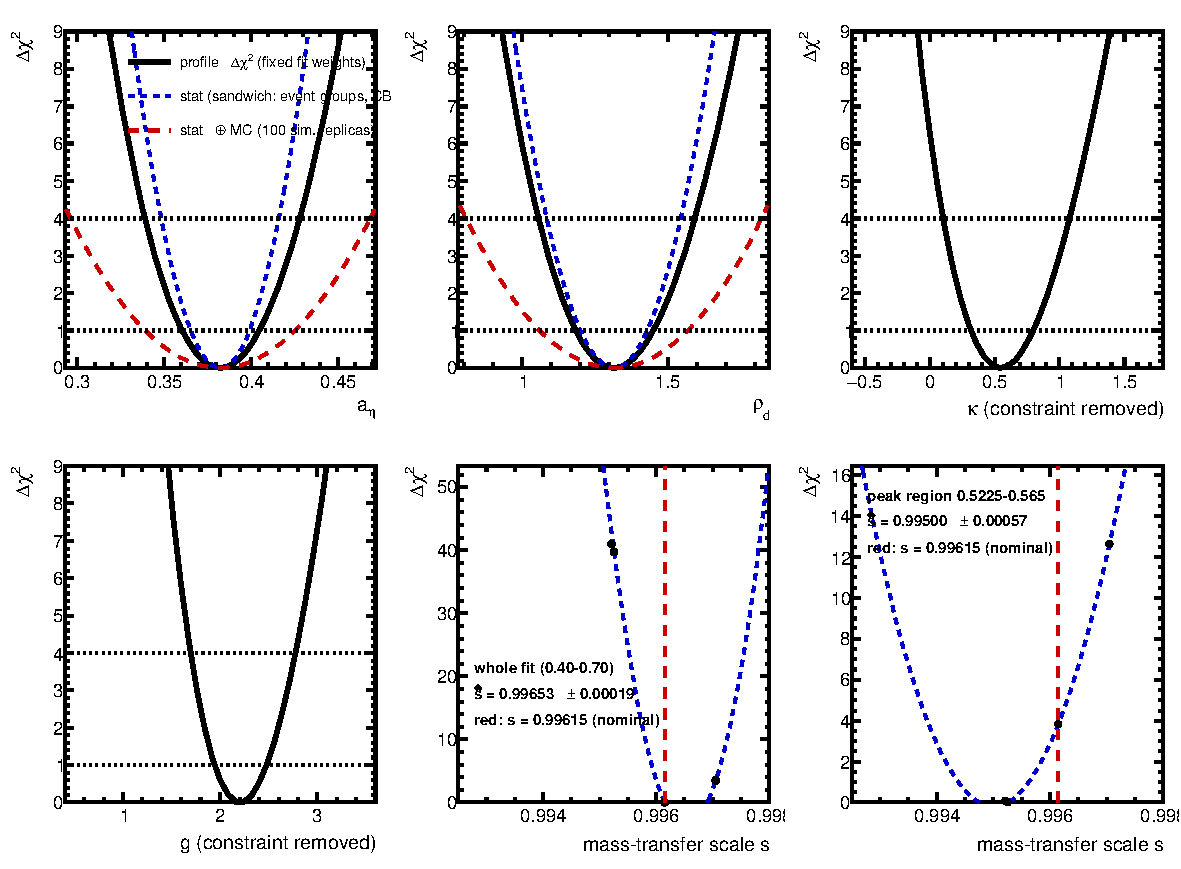
\includegraphics[width=0.8\textwidth]{figs_all/wp5_E3.pdf}
\caption{Spec.\ Fig.~E3: profile scans of the nominal F-main (CROSS-CHECK).
Selection: data, S0 (PT3 trigger, event vertex in the target region ($\vz>-160$\,mm), \betanew particle identification (pions within $3\sigma$, leptons within $5\sigma$ and with a RICH ring), energy-loss-corrected momenta of all four tracks, all stored combinations of each event (isBest $\ge0$), both pions in the event-vertex fit); F-main on \Mee$\ge10$\,\MeVcc in the \Mpipi slices $<0.34$, 0.34--0.37, 0.37--0.39, 0.39--0.43, $\ge0.43$\,\GeVcc, \Mfour 0.400--0.700\,\GeVcc (5\,\MeVcc bins, 2.5\,\MeVcc in 0.520--0.570) (350 bins); CB $=2\sqrt{N_{++}N_{--}}$ of the like-sign data with the same cuts (10\,\MeVcc cells of \Mfour, $k=1$), shared out by the like-sign share of each 50\,\MeVcc band; SMASH p+p at 4.5\,GeV (standard, lepton and $\eta$ sets, mode A) at its cross sections $\times$ PDG BR $\times$ the $\eta$-decay weights V3, masses moved to the data scale ($M_4'=0.99615\,M_4$, $\Mpipi'=0.9952\,\Mpipi$), same cuts; mass-scale scans over the whole fit range and over the peak region \Mfour 0.5225--0.565\,\GeVcc. $\Delta\chi^2$ with the weights frozen at the nominal fit (black) for
\aEta, \rhod, $\kappa$ and $g$ (the last two without their constraint); dashed: parabolas with the stat (sandwich) and the stat $\oplus$ MC
errors. Bottom middle/right: the mass-transfer scale $s$; points are refits with the factory templates at $s=0.99521$, 0.99525, 0.99615,
0.99705, the dashed line a parabola, red the nominal 0.99615; whole fit and peak region 0.5225--0.565\,\GeVcc. S0, isBest $\ge0$,
$L=6079.2\,\nbinv$. Fall-backs: E1 dropped ($\kappa=1\pm0.2$); template fits demoted to cross-checks.}
\label{fig:E3}
\end{figure}

\begin{figure}[H]
\centering
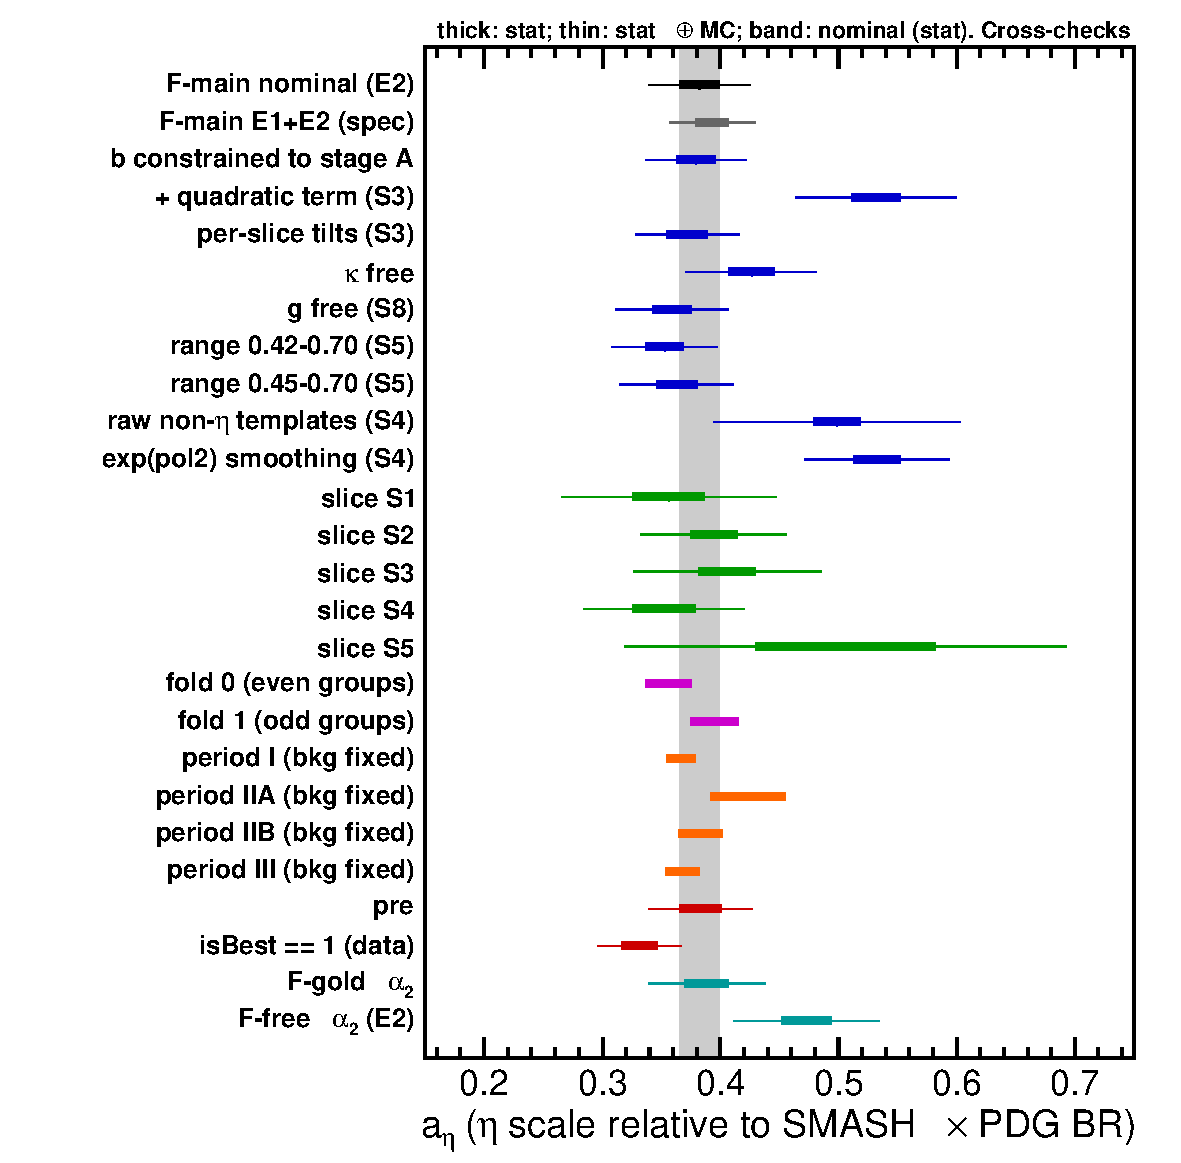
\includegraphics[width=0.66\textwidth]{figs_all/wp5_E4.pdf}
\caption{\aEta of every template fit: nominal, as specified, the variants, per slice, folds, periods, ``pre'', isBest $=1$, and
$\alpha_2$ of F-gold and F-free.
Selection: data, S0 (PT3 trigger, event vertex in the target region ($\vz>-160$\,mm), \betanew particle identification (pions within $3\sigma$, leptons within $5\sigma$ and with a RICH ring), energy-loss-corrected momenta of all four tracks, all stored combinations of each event (isBest $\ge0$), both pions in the event-vertex fit) unless stated; nominal: F-main on \Mee$\ge10$\,\MeVcc in the \Mpipi slices $<0.34$, 0.34--0.37, 0.37--0.39, 0.39--0.43, $\ge0.43$\,\GeVcc, \Mfour 0.400--0.700\,\GeVcc (5\,\MeVcc bins, 2.5\,\MeVcc in 0.520--0.570); as specified: both \Mee classes ($<10$, $\ge10$\,\MeVcc); folds: the two halves of the data by event-group parity; periods: days 034--046, 047--048, 049--053, 059--067; ``pre'': without the pion-vertex requirement; isBest $=1$: only the best-ranked combination per event (data only); F-gold: \Mee$\ge20$\,\MeVcc; CB $=2\sqrt{N_{++}N_{--}}$ of the like-sign data with the same cuts (10\,\MeVcc cells of \Mfour, $k=1$), shared out by the like-sign share of each 50\,\MeVcc band; SMASH p+p at 4.5\,GeV (standard, lepton and $\eta$ sets, mode A) at its cross sections $\times$ PDG BR $\times$ the $\eta$-decay weights V3, masses moved to the data scale ($M_4'=0.99615\,M_4$, $\Mpipi'=0.9952\,\Mpipi$), same cuts. Thick: stat; thin: stat $\oplus$ MC; grey band: nominal stat. All are cross-checks. S0 unless stated,
$L=6079.2\,\nbinv$. Fall-backs: E1 dropped ($\kappa=1\pm0.2$); template fits demoted to cross-checks.}
\label{fig:E4a}
\end{figure}

\begin{table}[H]
\centering
\caption{Acceptance criteria of stage B (specification WP5) as found by WP5 and by the verifier v5. Fall-backs: E1 dropped ($\kappa=1\pm0.2$); template fits demoted to cross-checks.}
\label{tab:wp5acc}
\small
\begin{tabular}{@{}p{4.0cm} p{6.2cm} p{5.0cm}@{}}
\toprule
criterion & value & verdict \\
\midrule
$\chi^2/\mathrm{ndf}\le1.2$ & GLS 2.59 (2.16 minimised); Pearson 3.40; hybrid GLS 1.90 (1.67) & FAIL; error scale 1.61 (1.38 hybrid), separate column \\
$|\rho(\aEta,b)|<0.7$ & 0.05 (stat + MC), 0.28 (stat) & PASS \\
per-slice \aEta $p>0.01$ & 0.92 (stat + MC), 0.11 (stat) & PASS \\
no pull run $>4$ bins in 0.52--0.56 & longest same-sign run S1 8, S2 3, S3 5, S4 6, S5 4 & FAIL (3 of 5 slices; S1 low by 1.6--2.5$\sigma$ in 0.52--0.55: a background level offset) \\
free $s$ within 2$\sigma$ of 0.99615 & $+1.95\sigma$ (whole fit), $-2.01\sigma$ (peak region) & PASS marginal (WP5) / MARGINAL, minimum not bracketed (v5) \\
folds $p>0.05$ & joint $p=0.55$ & PASS \\
\bottomrule
\end{tabular}
\end{table}

%======================================================================
\section{Side-band estimators and cross-checks (main results)}
\label{sec:sb}
%======================================================================
\inshort{the main result of the report: the $\eta$ peak yield $\Ypeak=5088\pm432\,(\mathrm{stat})\pm584\,(\mathrm{syst})\pm245\,(\mathrm{MC})$ counts, 0.418 of SMASH. The background-subtracted bump area (B4) rests on a background extrapolated from above the peak and is not determined; the bump itself is measured through its kinematic edge in \S\ref{sec:bedge}. The cross-checks of the $\eta$ scale lie at 0.36--0.45 of SMASH.}
\notebox{\textbf{Results} (S0, isBest $\ge0$, $L=6079.2\,\nbinv$, raw counts $\times64/63$, not efficiency corrected; ratios to SMASH with the
PDG 2020 BRs of the simulation, PDG 2026 values in Table~\ref{tab:P2}).\\
\textbf{Main result}: $\Ypeak$ (peak side bands, all \Mee) $=5088\pm432\,(\mathrm{stat})\pm584\,(\mathrm{syst})\pm245\,(\mathrm{MC})$;
closure term $\sigma_{\mathrm{tr}}=239^{+254}_{-239}$ counts.\\
\textbf{Main bump estimator by fall-back, but NOT DETERMINED}: \Ybump (B4, \Mee$\ge10$\,\MeVcc) $=7822\pm456\pm12\,870\,(165\,\%)\pm1920$;
all \Mee (extrapolated with the simulated \Mee shape, the yield used for DR and in Table~\ref{tab:S1}) $16\,389\pm1129\pm25\,770\,(157\,\%)\pm4110$.
The B4 background is \textbf{extrapolated} from CR-U and \textbf{not under control}: with a linear tilt the prediction lies above the
data in every region below the peak, with an added quadratic term below it, and \Ybump(E2) moves to 19\,526 ($+150$\,\%). The bump is
measured instead through its kinematic edge, which this term moves by only $-2$\,\% (\S\ref{sec:bedge}).\\
$\eta$-scale estimates relative to SMASH (\textbf{consistent cross-checks with a shared normalisation}: all use the S0 counts, $L$, the simulated
efficiencies including the event-vertex survival (0.9997 for the simulated $\eta$, $0.994\pm0.021$ measured in the data,
\S\ref{sec:vertexeff}), and the SMASH kinematics; F-main, the side bands and \Pmain share the data of P):
peak/SMASH $0.418\pm0.043$, F-main $\aEta=0.382\pm0.043$, $f_\eta$(edge) $0.392\pm0.050$ (errors of the first version; the measurement of
\S\ref{sec:bedge} gives $0.392\pm0.021\pm0.035\pm0.042$, 0.423 with the C2 angle corrected; in $u$, \S\ref{sec:edgeu}: 0.426), $f_\eta$(tag)
$0.454\pm0.043$ (emulated simulated tag; its acceptance verified, its photon-energy scale not, \S\ref{sec:ecalacc}), \Pmain 0.403 ($r_{\mathrm{res}}=1$) and 0.363 at the data-favoured $r_{\mathrm{res}}=0.89$; $a_B(E2)=0.312\pm0.079$ (not
determined, syst 168\,\%). The direct-decay and the conversion parts of the peak give 0.50 and 0.24 (\S\ref{sec:p2}).}

\subsection{Inputs and stage A at the fitted \texorpdfstring{$\eta$}{eta} values}
WP6 writes every S0 data entry (us, pp, mm) into a small tree so that windows of any width are counted with exact edges, and fills the
simulated window sums (C2--C5, \Geta, $G_D$, $G_C$, $T_{12}$ per slice and class) with their event-group variances and the 100 replicas of
WP0 (same generator and seed). All inputs reproduce the factory and the earlier packages exactly (window counts, CB to $10^{-10}$, replica
rms, F-main to $4\times10^{-8}$, the data edge step $1141.9\pm59.2\pm236$, the tag $3090.3\pm94.3$, \Pmain $4387.8\pm306.6\pm1078.2$).

Stage A is rerun with the $\eta$ terms at the F-main values ($a=0.382$, $\kappa=0.832$, $\rho=1.315$, $g=1.717$), as the specification asks
(WP3 used $a=0.4$, $g=1$), in the frozen WP3 configuration and with WP3's smoothing:

\begin{table}[H]
\centering
\caption{Stage A at the F-main $\eta$ values (first row, statistical errors in the second) compared with the same code at the WP3 $\eta$
values and with the frozen WP3 result. Model M1, E2, CR-U 0.575--0.700, \kEtwo$=1\pm0.05$. Fall-backs: E1 dropped, CR-K dropped (stage A from CR-U 0.575--0.700 only).}
\label{tab:stageA6}
\small
\begin{tabular}{@{}l r r r r r r r r@{}}
\toprule
 & $c_1$ & $c_2$ & $c_3$ & $c_4$ & $c_5$ & $b$ & \kB & \kEtwo \\
\midrule
$\eta$ at F-main & 0.9816 & 0.9844 & 0.9505 & 1.0473 & 0.9145 & $-0.0639$ & 2.932 & 0.955 \\
stat & 0.041 & 0.042 & 0.042 & 0.041 & 0.033 & 0.0058 & 0.269 & 0.048 \\
$\eta$ of WP3 ($a=0.4$, $g=1$) & 0.9917 & 1.0050 & 0.9746 & 1.0582 & 0.9113 & $-0.0661$ & 3.024 & 0.954 \\
WP3 frozen & 0.9878 & 1.0012 & 0.9751 & 1.0552 & 0.9091 & $-0.0683$ & 3.063 & 0.954 \\
\bottomrule
\end{tabular}
\end{table}

The WP3 values are reproduced within 0.1$\sigma$ (the rest comes from the weights: WP3 includes the $\eta$-template variance). GLS
$\chi^2$/ndf $=172.8/118=1.46$ (an upper estimate: the covariance holds only the smoothed-background replicas); with the WP4 smoothing
(start at 0.400 instead of the kinematic threshold) 1.56. The background in B (E2) is $B_A(\mathrm{B})=37\,763$ counts, in U (0.575--0.700)
296\,527. \flag{The two smoothings (WP3 for stage A, WP4 for F-main) differ by about 3.5\,\% on $c_j$ and 1\,\% on $B_A$(B) (v5); the WP4
smoothing is a family-S4 variant of B4 ($+4.6$\,\%).}

\subsection{The bump: estimator B4}
\label{sec:b4}
\textbf{In plain words.} Take the data minus the CB in the bump window; subtract the background, which is the data minus the CB minus the
$\eta$ content in the upper region U (0.575--0.700) carried down into B with the stage-A background shape; subtract the other $\eta$ classes in
B (C4, C5, \Geta at the F-main values):
\begin{equation}
\Ybump=\tfrac{64}{63}\Big\{(N-\mathrm{CB})_{\mathrm{B}}-\big[(N-\mathrm{CB})_{\mathrm{U}}-\eta_{\mathrm{U}}\big]\,\frac{B_A(\mathrm{B})}{B_A(\mathrm{U})}
-\big[a\kappa\,\mathrm{C4}+a\rho\,\mathrm{C5}+ag\,\Geta\big]_{\mathrm{B}}\Big\}.
\label{eq:b4}
\end{equation}
It is evaluated in E2 (stage A exists only there) and extrapolated to all \Mee with the simulated share
$f_{E2}=(\mathrm{C2}+\kappa\,\mathrm{C3})_{E2}/(\mathrm{C2}+\kappa\,\mathrm{C3})_{\mathrm{all}}=0.4773$ in B. \flag{Deviation: $\eta_{\mathrm{U}}$ (mostly
\Geta, 4.7\,\% of $(N-\mathrm{CB})_{\mathrm{U}}$) is subtracted before the extrapolation, as WP4 implemented and validated it; the formula of the
specification without it gives $-24$\,\%. Approved by the analyst on 15 November 2026 (D27).}

\textbf{Ingredients} (E2): $N_{\mathrm{B}}=53\,241$, CB$_{\mathrm{B}}=5667.8$; $N_{\mathrm{U}}=342\,098$, CB$_{\mathrm{U}}=32\,696.3$;
$\eta_{\mathrm{U}}=14\,399$ (\Geta 14\,375 at $ag=0.656$); $R=B_A(\mathrm{B})/B_A(\mathrm{U})=0.12735$; other $\eta$ in B 2305 (C4 12, C5 115, \Geta
2178). \textbf{Result}: $\Ybump(E2)=7822\pm456\,(\mathrm{stat})\pm1920\,(\mathrm{MC})$; stat $=$ $N$ 250 $\oplus$ CB 87 $\oplus$ stage A 368 $\oplus$
F-main 47; MC shift $-816$, bias-corrected 8638. All \Mee: $16\,389\pm1129\pm4110$, with an extrapolation uncertainty $+1196/-1356$ from
$\kappa=0.832\pm0.304$ ($f_{E2}$ 0.4448--0.5203). The \Mee share is supported by the ECAL-tagged $\eta$: its E2 share is $0.458\pm0.011$ in
data, 0.426 (fit) / 0.439 (truth) in the simulation. In SMASH units there are two bump scales, which must not be mixed:
$a_B(E2)=\Ybump(E2)/(\mathrm{C2}+\mathrm{C3})_{E2}=7822/25\,097=0.312\pm0.018\pm0.076$ ($\kappa=1$ in the denominator) and
$a_B(\mathrm{all})=\Ybump(\mathrm{all})/(\mathrm{C2}+\mathrm{C3})_{\mathrm{all}}=16\,389/54\,759=0.299\pm0.021\pm0.075$ (numerator extrapolated
with $f_{E2}$ at $\kappa=0.832$, denominator at $\kappa=1$). B4 is
\textbf{simulation-limited}: the MC error, 25\,\% of \Ybump(E2), comes from the template noise of the shape ratio $B_A(\mathrm{B})/B_A(\mathrm{U})$
(about 5\,\%).

\begin{table}[H]
\centering
\caption{Variants of B4 (E2) and of the peak side bands, value $\pm$ stat $\pm$ MC. Source: WP6 (\code{wp6_tableE3.txt}). Fall-backs: E1 dropped (B4 in E2), CR-K dropped (bump extrapolated).}
\label{tab:sbvar}
\footnotesize
\begin{tabular}{@{}l r r@{}}
\toprule
variant & value & change \\
\midrule
\multicolumn{3}{@{}l}{\emph{B4, \Mee$\ge10$\,\MeVcc (nominal $7822\pm456\pm1920$)}} \\
without the $\eta_{\mathrm{U}}$ subtraction (specification literal) & $5959\pm482\pm2079$ & $-24$\,\% \\
CB $\times$ \kEtwo of stage A & $7891\pm447\pm1931$ & $+0.9$\,\% \\
per-slice transfer & $7810\pm461\pm1919$ & $-0.2$\,\% \\
normalised on U 0.565--0.700 (same stage A) & $7867\pm449\pm1895$ & $+0.6$\,\% \\
stage A and U on 0.565--0.700 & $8213\pm424\pm1717$ & $+5.0$\,\% \\
stage A with the WP4 smoothing & $8182\pm460\pm2056$ & $+4.6$\,\% \\
WP3 frozen stage A ($\eta$ 0.4, $g=1$) & $7389\pm452\pm1597$ & $-5.5$\,\% \\
\textbf{stage A + quadratic term} ($q=-0.173\pm0.022$) & $\mathbf{19\,526\pm1434\pm3919}$ & $\mathbf{+150}$\,\% \\
E1+E2 direct (E1 shape predicted with the E2 parameters; test only) & $12\,256\pm884\pm3738$ & \\
per slice S1 / S2 / S3 / S4 & 1567 / 3426 / 2055 / 878 & \\
per slice S5 (no bump: null test) & $\mathbf{-117\pm21\pm52}$ & $-2.1\sigma$ \\
\midrule
\multicolumn{3}{@{}l}{\emph{Peak side bands, all \Mee (nominal $5088\pm432\pm245$)}} \\
per class (E1 + E2 separately) & $5159\pm438\pm250$ & $+1.4$\,\% \\
only the background normalised by the side bands & $5112\pm432\pm273$ & $+0.5$\,\% \\
leakage shape $\kappa$C4 + $\rho$C5 & $5100\pm433\pm240$ & $+0.2$\,\% \\
no leakage correction ($f=0$) & $4156\pm353\pm192$ & $-18$\,\% \\
narrow side bands (5.6\,\MeVcc) & $4733\pm510\pm301$ & $-7.0$\,\% \\
wide side bands (11.6\,\MeVcc) & $4745\pm388\pm225$ & $-6.7$\,\% \\
flat background ($R'=$ width ratio) & $4733\pm433$ & $-7.0$\,\% \\
stage A + quadratic term & $5263\pm431\pm293$ & $+3.4$\,\% \\
stage A with the WP4 smoothing & $5068\pm432\pm244$ & $-0.4$\,\% \\
stage A on 0.565--0.700 & $5093\pm432\pm245$ & $+0.1$\,\% \\
WP3 frozen stage A & $5073\pm432$ & $-0.3$\,\% \\
\bottomrule
\end{tabular}
\end{table}

\subsection{The peak: side-band estimator}
\textbf{In plain words.} Take the data minus the CB in the peak window P; subtract the data minus the CB of the two side bands, scaled by the
expected ratio $R'$ of the non-peak content in P and in the side bands; because the $\eta$ peak itself leaks into the side bands (a share $f$
of it, from the simulated C4+C5 shape), divide by $1-R'f$:
\begin{equation}
Y_{\mathrm{peak}}=\tfrac{64}{63}\,\frac{(N-\mathrm{CB})_{\mathrm{P}}-R'\,(N-\mathrm{CB})_{\mathrm{SB}}}{1-R'f},
\label{eq:sb}
\end{equation}
\[
R'=\frac{\big[B_A+a(\mathrm{C2}+\kappa\mathrm{C3})+ag\,G_\eta\big]_{\mathrm{P}}}{\big[B_A+a(\mathrm{C2}+\kappa\mathrm{C3})+ag\,G_\eta\big]_{\mathrm{SB}}},\qquad
f=\frac{(\mathrm{C4}+\mathrm{C5})_{\mathrm{SB}}}{(\mathrm{C4}+\mathrm{C5})_{\mathrm{P}}}.
\]
This is the closed form of ``iterating the leakage out'': $Y_{n+1}=(N-\mathrm{CB})_{\mathrm{P}}-R'[(N-\mathrm{CB})_{\mathrm{SB}}-fY_n]$ gives
4091.5, 4840.6, 4977.7, 5002.8, 5007.4, 5008.3 raw counts and converges to 5008.5 ($\times64/63=5088.0$). \textbf{Ingredients}:
$N_{\mathrm{P}}=55\,947$, CB$_{\mathrm{P}}=3279.0$; $N_{\mathrm{SB}}=43\,656$, CB$_{\mathrm{SB}}=2695.0$; $B_A$(P) 59\,210, $B_A$(SB) 49\,859;
bump tail + \Geta 2435 in P and 2121 in SB; $R'=1.1859$ (background alone 1.1875, flat background 1.1930); $f=0.1544$.

\textbf{Result}: $\Ypeak=5088\pm432\,(\mathrm{stat})\pm245\,(\mathrm{MC})$ (stat $=N$ 426 $\oplus$ CB 69 $\oplus$ stage A 6 $\oplus$ F-main 9;
MC shift $-36$); per class E1 $2380\pm291\pm164$, E2 $2780\pm326\pm179$, E2 share $0.546\pm0.046\pm0.027$. Visible yield
$\sigma_{\mathrm{vis}}=\Ypeak/L=0.837\pm0.071\pm0.040$ visible counts per \nbinv; peak/SMASH (C4+C5) $=\aP=0.418\pm0.035\pm0.025$. The estimator is robust to the background model (the stage-A part
of its error is 6 counts) but sensitive to the side-band width ($-7$\,\%, within the correlated statistical error) and to the leakage
correction ($+22$\,\%, from the simulated peak shape, whose width is 6.1\,\MeVcc against 5.4\,\MeVcc in the data). It is not
simulation-limited (MC/stat $=0.57$).

\textbf{Double ratio.} DR $=\aP/a_B(\mathrm{all})=0.418/0.299=1.40\pm0.15\pm0.53$ (MC shift $+0.31$, bias-corrected 1.09; 1.373 with
PDG 2026). The $\kappa$ convention matters at the level of the statistical error: with $\kappa=1$ everywhere (extrapolation and denominators)
DR $=0.418/0.312=1.34$, with $\kappa=0.832$ everywhere (also in \aP) about 1.41. Both in E2: $1.73\pm0.23\pm0.61$. DR is derived from the
undetermined B4 bump area (syst 67\,\%) and is \textbf{not determined}; F-main gives $1.17\pm0.15$. Through the bump edge the double ratio is
determined: $\mathrm{DR}_{\mathrm{edge}}=0.97\pm0.10\pm0.17\pm0.12$ (\S\ref{sec:bedge-cmp}).

\subsection{Closure tests}
\label{sec:closure}
\textbf{Displaced windows.} The side-band estimator is applied at 13 window centres 0.575, 0.585, \dots, 0.695\,\GeVcc, where there is no
$\eta$; for each, the window and its side bands are removed from CR-U and stage A is refitted; the pull is $(Y-Y_{\mathrm{exp}})/\sigma_{\mathrm{stat}}$,
with $Y_{\mathrm{exp}}$ the simulated C4+C5 content passed through the same estimator. Pulls: $+0.97$, $+0.12$, $-0.49$, $-0.38$, $+0.84$, $-0.78$,
$+1.94$, $+1.10$, $-1.17$, $+2.29$, $+0.64$, $+0.08$, $+1.53$; rms 1.143 (mean $+0.51$); without the refit 1.181, in E2 alone 1.572. Hence
$\sigma_{\mathrm{tr}}=\sigma_{\mathrm{stat}}\sqrt{\mathrm{rms}^2-1}=431.6\times\sqrt{1.143^2-1}=239$ counts $=4.7$\,\% of \Ypeak: the family-S10 entry of
the peak. The windows overlap (10\,\MeVcc steps, 37.8\,\MeVcc wide), so the pulls are correlated; at 0.575 the lower side band holds the tail of
the real peak ($Y_{\mathrm{exp}}=-279$). \textbf{Precision of the rms} (review, \code{fix_numbers.py}): the 13 windows are about $n_{\mathrm{eff}}=3.4$
independent ones, so $\mathrm{rms}^2=1.31\pm1.00$, rms $1.14^{+0.37}_{-0.59}$ and $\sigma_{\mathrm{tr}}=239^{+254}_{-239}$ counts; the four
interleaved sets of non-overlapping windows give rms 1.16, 1.40, 1.21, 0.67 ($\sigma_{\mathrm{tr}}=251$, 422, 296, 0 counts); the mean pull
$+0.51\pm0.62$ is not significant. With the upper value (493 counts, 9.7\,\%) the \Ypeak systematic would be 14.2\,\% instead of 11.5\,\%; the
nominal 239 counts is kept. In E2 alone the rms is 1.572, i.e.\ $\sigma_{\mathrm{tr}}(E2)=326\times\sqrt{1.572^2-1}=395$ counts (14\,\% of the E2
yield); it is applied to the per-class yields used for the composition of the peak (\S\ref{sec:p2}).

\textbf{Prediction pulls below the peak} (E2; prediction $=k\,\mathrm{CB}+B_A+\eta$(F-main)):

\begin{table}[H]
\centering
\caption{Closure of the bump background (E2). S10 term $=\max(|N-\mathrm{pred}|,\sigma_{\mathrm{pred}})$, transferred to the bump as the same
relative error on the B4 background in B. Lower part: pulls of the same regions with two other stage-A variants. Fall-backs: CR-K dropped; the CR-L term is the S10 entry required by the fall-back.}
\label{tab:bclos}
\small
\resizebox{\textwidth}{!}{%
\begin{tabular}{@{}l r r r r r r@{}}
\toprule
region & $N$ & prediction (stat, MC) & pull & S10 term & as \% of $B_A$ & on \Ybump(E2) \\
\midrule
CR-L 0.5225--0.5300 & 7519 & 8018 (59, 244) & $-1.88$ & 499 & 7.7\,\% & 2931 counts $=$ \textbf{37.5\,\%} \\
CR-K (S5, 0.400--0.5225) & 331 & 441 (11, 51) & $-1.98$ & 110 & 37.8\,\% & 14\,436 $=185$\,\% \\
0.400--0.455 (below B) & 13\,786 & 16\,086 (173, 801) & $-2.78$ & 2300 & 18.4\,\% & 7025 $=90$\,\% \\
\midrule
stage A + quadratic: pulls & & & $+1.62$ / $-1.01$ / $+1.74$ & & & \\
stage A, WP4 smoothing: pulls & & & $-1.56$ / $-3.08$ / $-2.54$ & & & \\
\bottomrule
\end{tabular}}
\end{table}

With the linear tilt the background predicted below the peak is too high (CR-L $-6$\,\%, CR-K $-25$\,\%, 0.400--0.455 $-14$\,\% as
data/prediction $-1$); with a quadratic term it is too low. The true background in B lies between the two (a linear interpolation to zero CR-L
pull would give about 12\,900 counts, information only). The CR-L term (37.5\,\%) is the family-S10 entry required by the fall-back; the region
below B suggests up to 90\,\%. The S5 null test of B4 ($-117\pm56$, $-2.1\sigma$) has the same sign as the CR-K pull.

\subsection{Cross-checks: edge step, ECAL tag, \texorpdfstring{\Pmain}{P\_main}}
\label{sec:xcheck}
\textbf{Edge step} (Fig.~\ref{fig:edge}). The frozen procedure of Part~II (pol2 [+ $\eta$ Gaussian] + step $h$ at the fixed edge
$0.99277\,M_4^{\max}(\Mpipi/0.9970)$, smeared by 5.4\,\MeVcc, in the slices 0.30--0.34, 0.34--0.37, 0.37--0.39, 0.39--0.40\,\GeVcc) is applied
with \emph{the same fit} to the data and to the simulated $T_1+T_2$; $E$ is the sum of the four $h$.

\begin{table}[H]
\centering
\caption{Edge steps $h$ (counts per 2.5\,\MeVcc) of data S0 ($N-\mathrm{CB}$) and of the simulated $T_1+T_2$ (expected raw counts at SMASH). No fall-back involved.}
\label{tab:edge}
\small
\begin{tabular}{@{}l r r r@{}}
\toprule
\Mpipi [\GeVcc] & data $h$ & simulation $h$ & data/sim \\
\midrule
0.30--0.34 & $287\pm37$ & 841 & 0.342 \\
0.34--0.37 & $389\pm33$ & 847 & 0.459 \\
0.37--0.39 & $331\pm24$ & 882 & 0.376 \\
0.39--0.40 & $135\pm22$ & 346 & 0.389 \\
sum $E$ & $1141.9\pm59.2$ (fit) & 2915.7 & 0.392 \\
\bottomrule
\end{tabular}
\end{table}

$f_\eta(\mathrm{edge})=E_{\mathrm{data}}/E_{\mathrm{sim}}=0.392\pm0.024\,(\mathrm{stat})\pm0.039\,(\mathrm{MC})\pm0.021\,(\mathrm{model})$; the
statistical error includes the factor 1.2 of the Part~II calibration with independent halves (\S7.2 there; WP6 quoted 0.020 before it). The
model error comes from 18 variations (order 2/3, half range 35/45/55\,\MeVcc, smearing 4.4/5.4/6.4\,\MeVcc) applied jointly to data and
simulation. By class (statistical errors also $\times1.2$): E1 $0.367\pm0.029\pm0.045\pm0.076$, E2 $0.431\pm0.043\pm0.073\pm0.073$. The simulated step comes from the bump classes
(C2+C3 alone 3010; the rest of $T_1+T_2$ gives 40.6, 1.4\,\%). Control slices: 0.40--0.41 data $18.7\pm14.7$ (simulation 116); 0.42--0.46
data $15.4\pm15.0$ (simulation $-14.5$). This ratio needs no background normalisation and is the robust bump-scale check. It is turned into a
measurement in \S\ref{sec:bedge}: there the statistical error comes from 200 bootstrap copies of the data (0.021; the factor 1.2 of the Part~II
calibration is not confirmed), the MC error from the replica spread of the ratio (0.042), the systematic error from 43 variants (0.032), and the
estimator is tested on pseudo-data; in the distance to the edge, $u$, it is measured with one fit in \S\ref{sec:edgeu}.

\textbf{ECAL tag} (Fig.~\ref{fig:tag}): good photon, $M(\ee\gamma)$ 0.119--0.173, \Mee$<0.10$\,\GeVcc; data $T$ from the frozen m5c fit
(0.5463 / 6.2\,\MeVcc, pol2): $3090.3\pm94.3$ (all \Mfour; Part~II gives $3088\pm94$ for ``pre + vertex'', Table opt\_named: the same within
2 counts). The positive control of WP3 ($M_4<0.5225$, \Mpipi$<0.43$: $T=3253\pm92$) is larger than this although it is a subset: each $T$ is the
Gaussian content of its own fit with its own pol2 background, and the subset has a different background under the m5c peak, so the two fits
are not additive (Part~II found the same: the subset $M_4<0.5225$ gives a share 1.05, uncertain by about 0.1). The simulated tag is emulated
with the same combinations and fit: 6804 ($\pm603$ MC);
$f_\eta(\mathrm{tag})=0.454\pm0.014\pm0.040$ (free shapes 0.434; bump region 0.465). \textbf{What is verified and what is not}: the emulation
of the simulated tag is reproduced entry by entry and its acceptance (geometry, module status, photon direction) is verified (\S\ref{sec:ecalacc});
the photon energy scale and the module efficiency are not, so the tag stays verification only. The simulated \piz in $M(\ee\gamma)$ sits at
0.1287 (8.0\,\MeVcc), the data at 0.1459 (13.25\,\MeVcc), i.e.\ \piz positions 4.7\,\% below (simulation) and 8\,\% above (data) $m_{\piz}$; these
are shifts of the \piz position, not the photon energy scales, which are about 7--9\,\% low in the simulation (cluster truth) and about 17\,\% high
in the data (rescaling factor 0.856; \S\ref{sec:ecalacc-data}). Re-centring the window on the simulation changes $f_\eta$(tag) by $-9$ to $-14$\,\%
(0.413 frozen fit, 0.372 free); the full prediction with a data-like energy scale is in \S\ref{sec:ecalacc}.

\textbf{\Pmain} (Part~II frozen Gaussian + pol2 fit of $N-\mathrm{CB}$ in 0.5225--0.6100): S0 $S=4388\pm307\,(\mathrm{stat})\pm420\,(\mathrm{model})$,
with the revised model uncertainty of Part~II (rms over the 144 edge-safe variations; the old envelope was $\pm1078$). In P, $\times64/63$: 4202.
The same frozen fit on the simulated $T_1+T_2$ gives 10\,881 ($r_{\mathrm{res}}=1$) and 12\,098 ($r_{\mathrm{res}}=0.89$), so $S_{\mathrm{data}}/S_{\mathrm{sim}}=0.403$ / 0.363
(information; no MC error; the free simulated width is 5.2\,\MeVcc at $r_{\mathrm{res}}=1$). The like-for-like value at the data-favoured
resolution ($r_{\mathrm{res}}=0.89$, \S\ref{sec:mscale}) is 0.363, not 0.403. For comparison, Part~II's recommended data-only numbers are
$S=4364\pm310\pm477$ (PEAK) and $4671\pm367\pm453$ (``pre''), and $E=1199\pm71\pm287$ (``pre''; Part~II has withdrawn its earlier $\pm85$ with the factor 1.2, since the bootstrap of
\S\ref{sec:bedge} confirms the fit error).

\begin{table}[H]
\centering
\caption{Spec.\ Table~E3: side-band estimators, closure and cross-checks. S0, isBest $\ge0$, $L=6079.2\,\nbinv$, raw counts $\times64/63$; ratios
to SMASH with the PDG 2020 BRs of the simulation (PDG 2026 values in Table~\ref{tab:P2}). syst from Table~\ref{tab:S1}. Fall-backs: E1 dropped
(B4 in E2, extrapolated with $f_{E2}$), CR-K dropped (bump background extrapolated), template fits demoted (side bands main), B4
simulation-limited. Source: WP6 (\code{wp6_tableE3.txt}), rewritten with full labels and the revised errors of the $f_\eta$(edge) statistics
($\times1.2$, Part~II calibration) and of the \Pmain model (edge-safe rms 420 instead of the old envelope 1078) (\code{tables_all/fix_tableE3.tex});
the syst of \aP is that of \sigeta without the composition term, with the peak tail of D40 (16.0\,\% $\oplus$ 8.8\,\%; 0.153 or 36.6\,\% with
the composition term), final review (\code{fix2_tableE3.tex}).}
\label{tab:E3}
\footnotesize
\resizebox{\textwidth}{!}{\tabin{fix2_tableE3_ra4.tex}}
\end{table}

\begin{figure}[H]
\centering
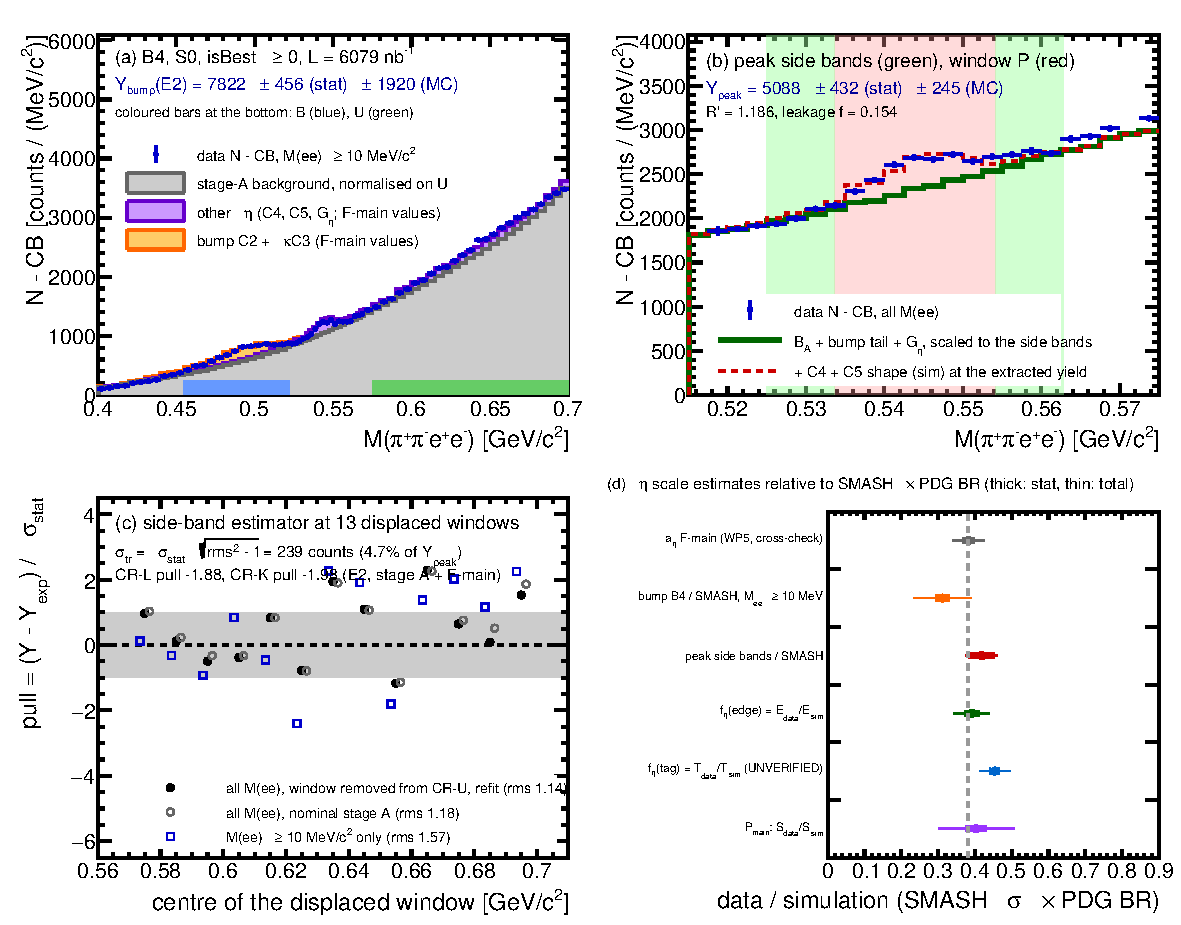
\includegraphics[width=0.86\textwidth,trim=0 222 0 0,clip]{figs_all/fix_wp6_E4_unrot_cnt.pdf}\\[0.2em]
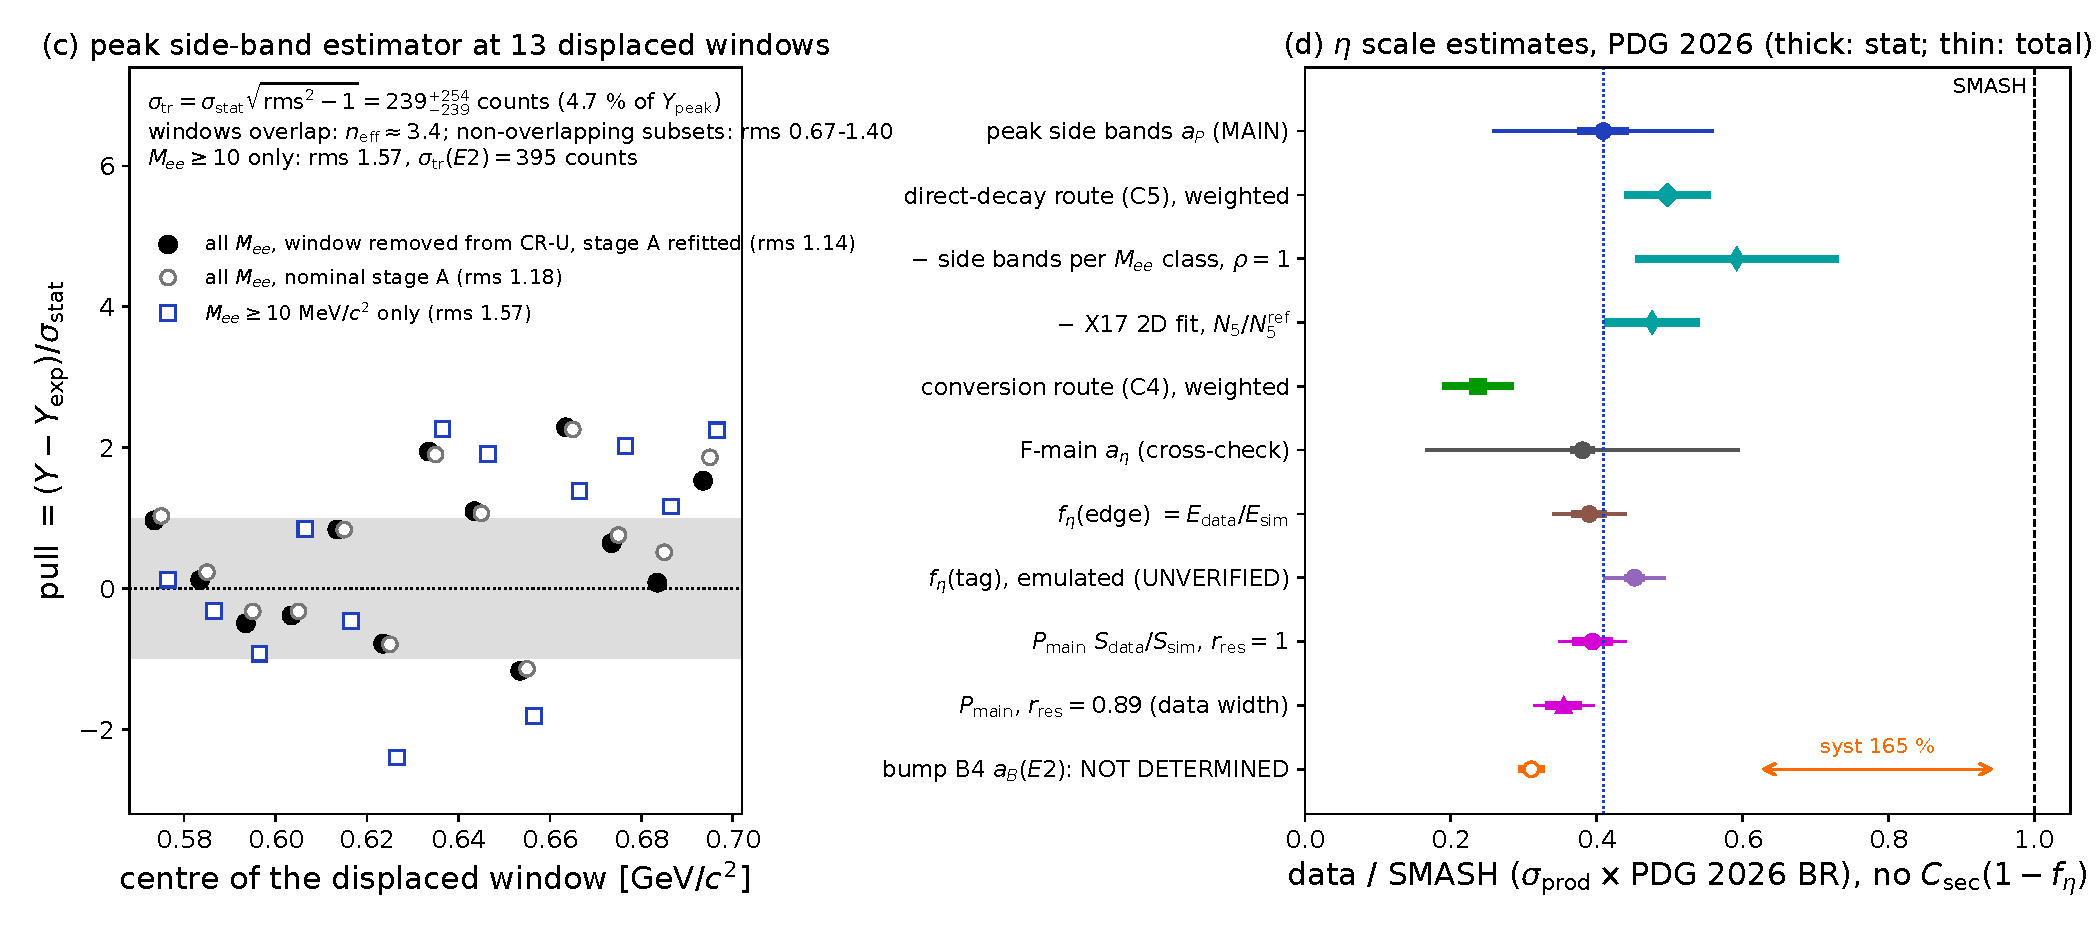
\includegraphics[width=0.88\textwidth]{figs_all/fix_E4cd_cnt.pdf}
\caption{Spec.\ Fig.~E4: side-band estimators and cross-checks.
Selection: data, S0 (PT3 trigger, event vertex in the target region ($\vz>-160$\,mm), \betanew particle identification (pions within $3\sigma$, leptons within $5\sigma$ and with a RICH ring), energy-loss-corrected momenta of all four tracks, all stored combinations of each event (isBest $\ge0$), both pions in the event-vertex fit); CB $=2\sqrt{N_{++}N_{--}}$ of the like-sign data with the same cuts (10\,\MeVcc cells of \Mfour, $k=1$), shared out by the like-sign share of each 50\,\MeVcc band; SMASH p+p at 4.5\,GeV (standard, lepton and $\eta$ sets, mode A) at its cross sections $\times$ PDG BR $\times$ the $\eta$-decay weights V3, masses moved to the data scale ($M_4'=0.99615\,M_4$, $\Mpipi'=0.9952\,\Mpipi$), same cuts. (a) \Mee$\ge10$\,\MeVcc, slices summed, F10 bins in \Mfour 0.40--0.70\,\GeVcc; bump window 0.4550--0.5225\,\GeVcc; background normalised in \Mfour 0.575--0.700\,\GeVcc (\Mee$\ge10$\,\MeVcc, the stage-A region). (b) all \Mee, \Mfour 0.515--0.575\,\GeVcc; peak window 0.53364--0.55416\,\GeVcc, side bands 0.5250--0.5336 and 0.5542--0.5628\,\GeVcc. (c) windows of the same widths (37.8\,\MeVcc in all) centred at 0.575, 0.585, \dots, 0.695\,\GeVcc; all \Mee (circles), \Mee$\ge10$\,\MeVcc (squares). (d) each estimate with its own windows: side bands as (b); F-main as Fig.~\ref{fig:E1}; bump edge in the \Mpipi slices 0.30--0.34, 0.34--0.37, 0.37--0.39, 0.39--0.40\,\GeVcc and in $u$; ECAL tag; \Pmain in 0.5225--0.6100\,\GeVcc; routes from the side bands per \Mee class and the X17 fit (\Mfour 0.5225--0.6100\,\GeVcc, \Mee 2--62\,\MeVcc). Data S0, isBest $\ge0$, $L=6079.2\,\nbinv$, raw counts. (a) B4, \Mee$\ge10$\,\MeVcc:
data $N-\mathrm{CB}$ (blue, CB spread rule) per \MeVcc summed over the slices; grey: stage-A background ($c_j(1+bx)[G_D+\kB G_C]$ fitted in CR-U
0.575--0.700) normalised to the data in U (green bar) and extrapolated into B (blue bar); violet: the other $\eta$ classes (C4, C5, \Geta at the
F-main values); orange: the bump C2+$\kappa$C3 at the F-main values (shape only). (b) Peak side bands, all \Mee, 2.5\,\MeVcc bins: green line, the
background ($B_A$ + bump tail + \Geta) scaled to the side bands (green bands) after removing the peak leakage; red dashed: plus the simulated
C4+C5 shape at the extracted yield; red band: window P. (c) Pulls of the side-band estimator at 13 displaced windows: full circles with the window
removed from CR-U and stage A refitted, open circles nominal stage A, squares \Mee$\ge10$\,\MeVcc only; grey band $\pm1$; the windows overlap
($n_{\mathrm{eff}}\approx3.4$). (d) $\eta$-scale estimates relative to SMASH $\sigma\times$PDG 2026 BR (thick: stat, thin: total), with the
revised errors; the routes of \S\ref{sec:p2}; $f_\eta$(tag) uses the emulated simulated tag (acceptance verified, photon-energy scale not,
\S\ref{sec:ecalacc}); B4 is not determined. Panels (a, b): WP6
(\code{wp6_E4.pdf}); panels (c, d) redrawn from WP6's numbers with the revised errors (\code{fix_figs.py}). Fall-backs: E1 and CR-K dropped,
template fits demoted.}
\label{fig:E4}
\end{figure}

\begin{figure}[H]
\centering
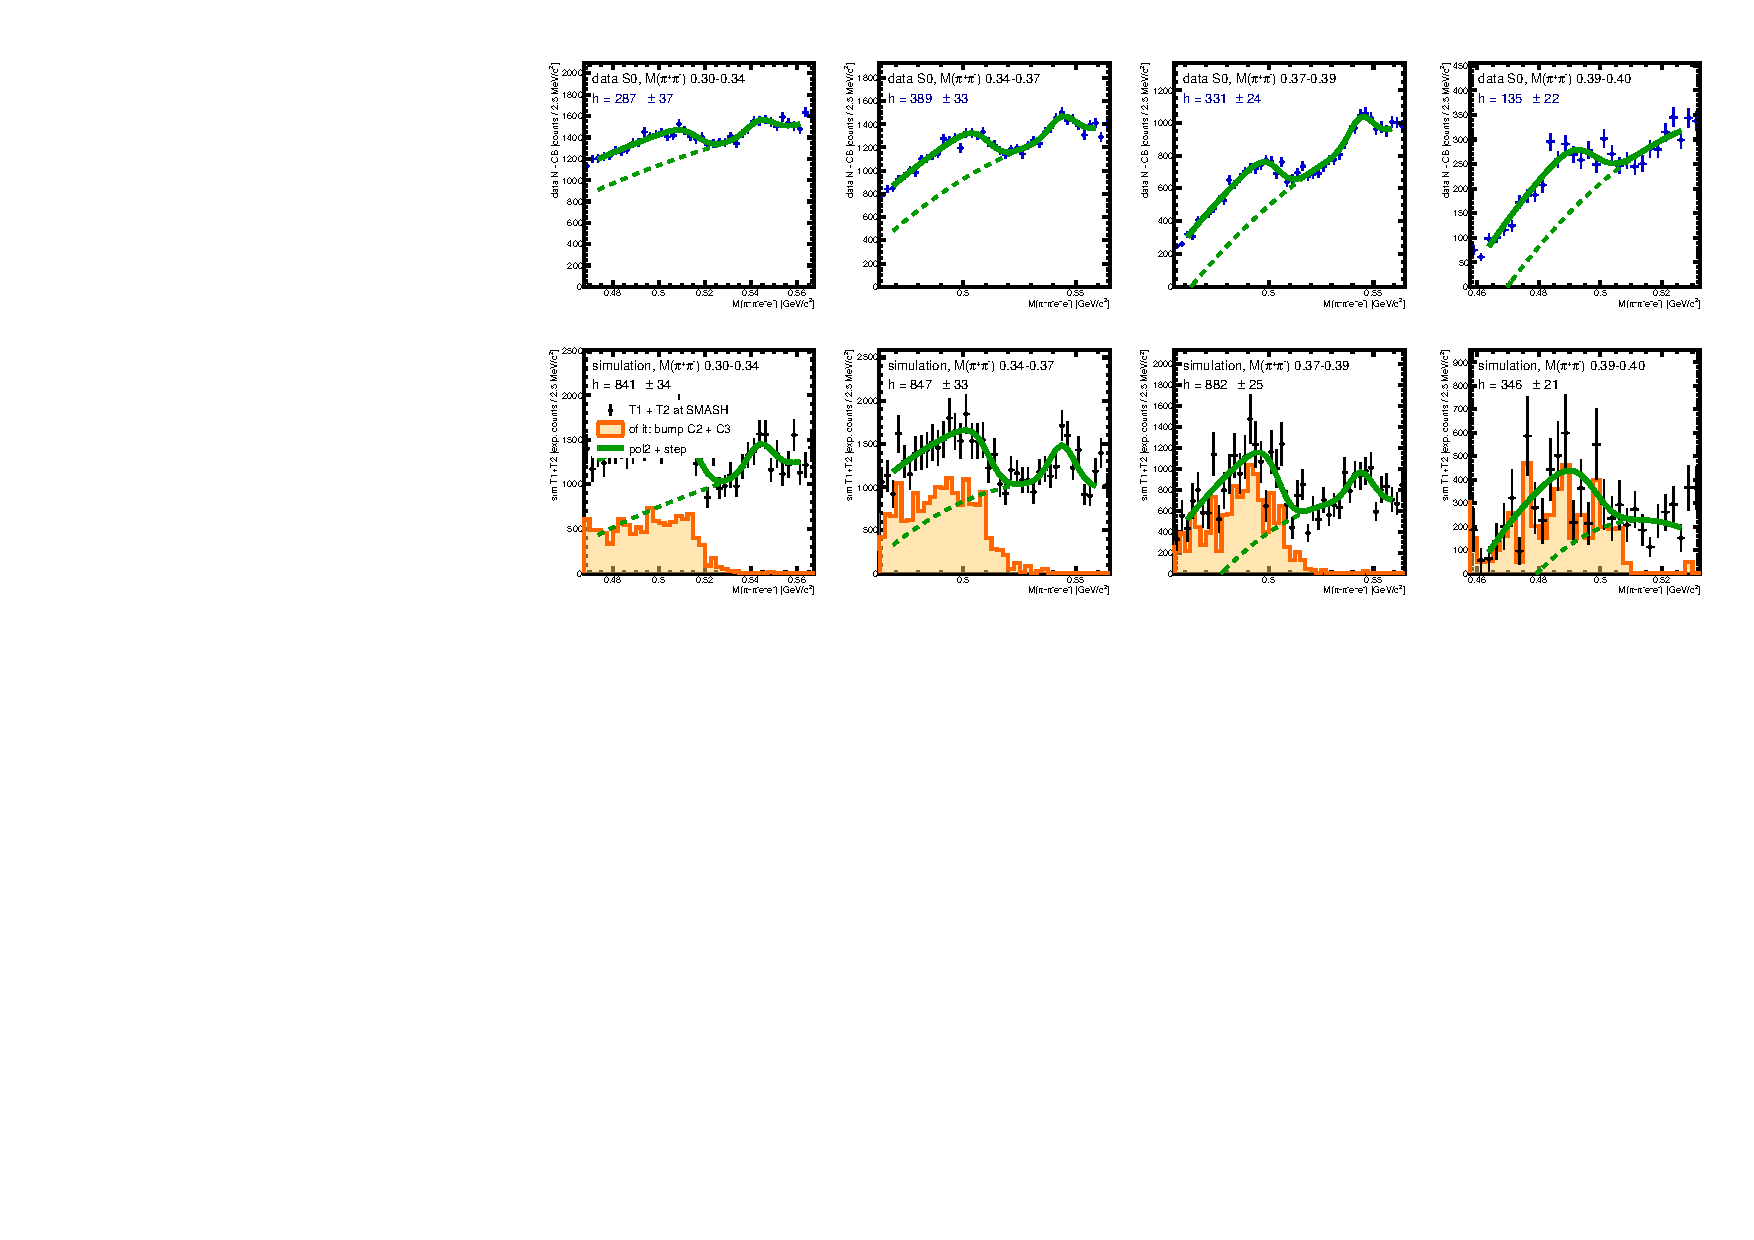
\includegraphics[width=\textwidth]{figs_all/wp6_edge_cnt.pdf}
\caption{Edge step of the bump in data and simulation.
Selection: data, S0 (PT3 trigger, event vertex in the target region ($\vz>-160$\,mm), \betanew particle identification (pions within $3\sigma$, leptons within $5\sigma$ and with a RICH ring), energy-loss-corrected momenta of all four tracks, all stored combinations of each event (isBest $\ge0$), both pions in the event-vertex fit), all \Mee, in the \Mpipi slices 0.30--0.34, 0.34--0.37, 0.37--0.39, 0.39--0.40\,\GeVcc; 2.5\,\MeVcc bins, fit range the edge $\pm45$\,\MeVcc ($\pm35$\,\MeVcc in 0.39--0.40), step smeared by 5.4\,\MeVcc; CB $=2\sqrt{N_{++}N_{--}}$ of each slice in 10\,\MeVcc cells, $k=1$ (own like-sign counts of the slice); simulation: $T_1+T_2$ of SMASH p+p at 4.5\,GeV (standard, lepton and $\eta$ sets, mode A) at its cross sections $\times$ PDG BR $\times$ the $\eta$-decay weights V3, masses moved to the data scale ($M_4'=0.99615\,M_4$, $\Mpipi'=0.9952\,\Mpipi$), same cuts, same fit. Top: data S0 $N-\mathrm{CB}$ in \Mpipi 0.30--0.34, 0.34--0.37, 0.37--0.39, 0.39--0.40\,\GeVcc,
counts per 2.5\,\MeVcc. Bottom: simulated $T_1+T_2$ at SMASH $\times$ PDG BR, expected raw counts ($L=6079.2\,\nbinv\times63/64$), event-group errors;
orange: the bump classes C2+C3. Green: frozen fit pol2 + $h\times$step at $0.99277\,M_4^{\max}(\Mpipi/0.9970)$, smearing 5.4\,\MeVcc; dashed:
without the step. $f_\eta(\mathrm{edge})=\sum h_{\mathrm{data}}/\sum h_{\mathrm{sim}}=0.392$. No fall-back involved.}
\label{fig:edge}
\end{figure}

\begin{figure}[!htb]
\centering
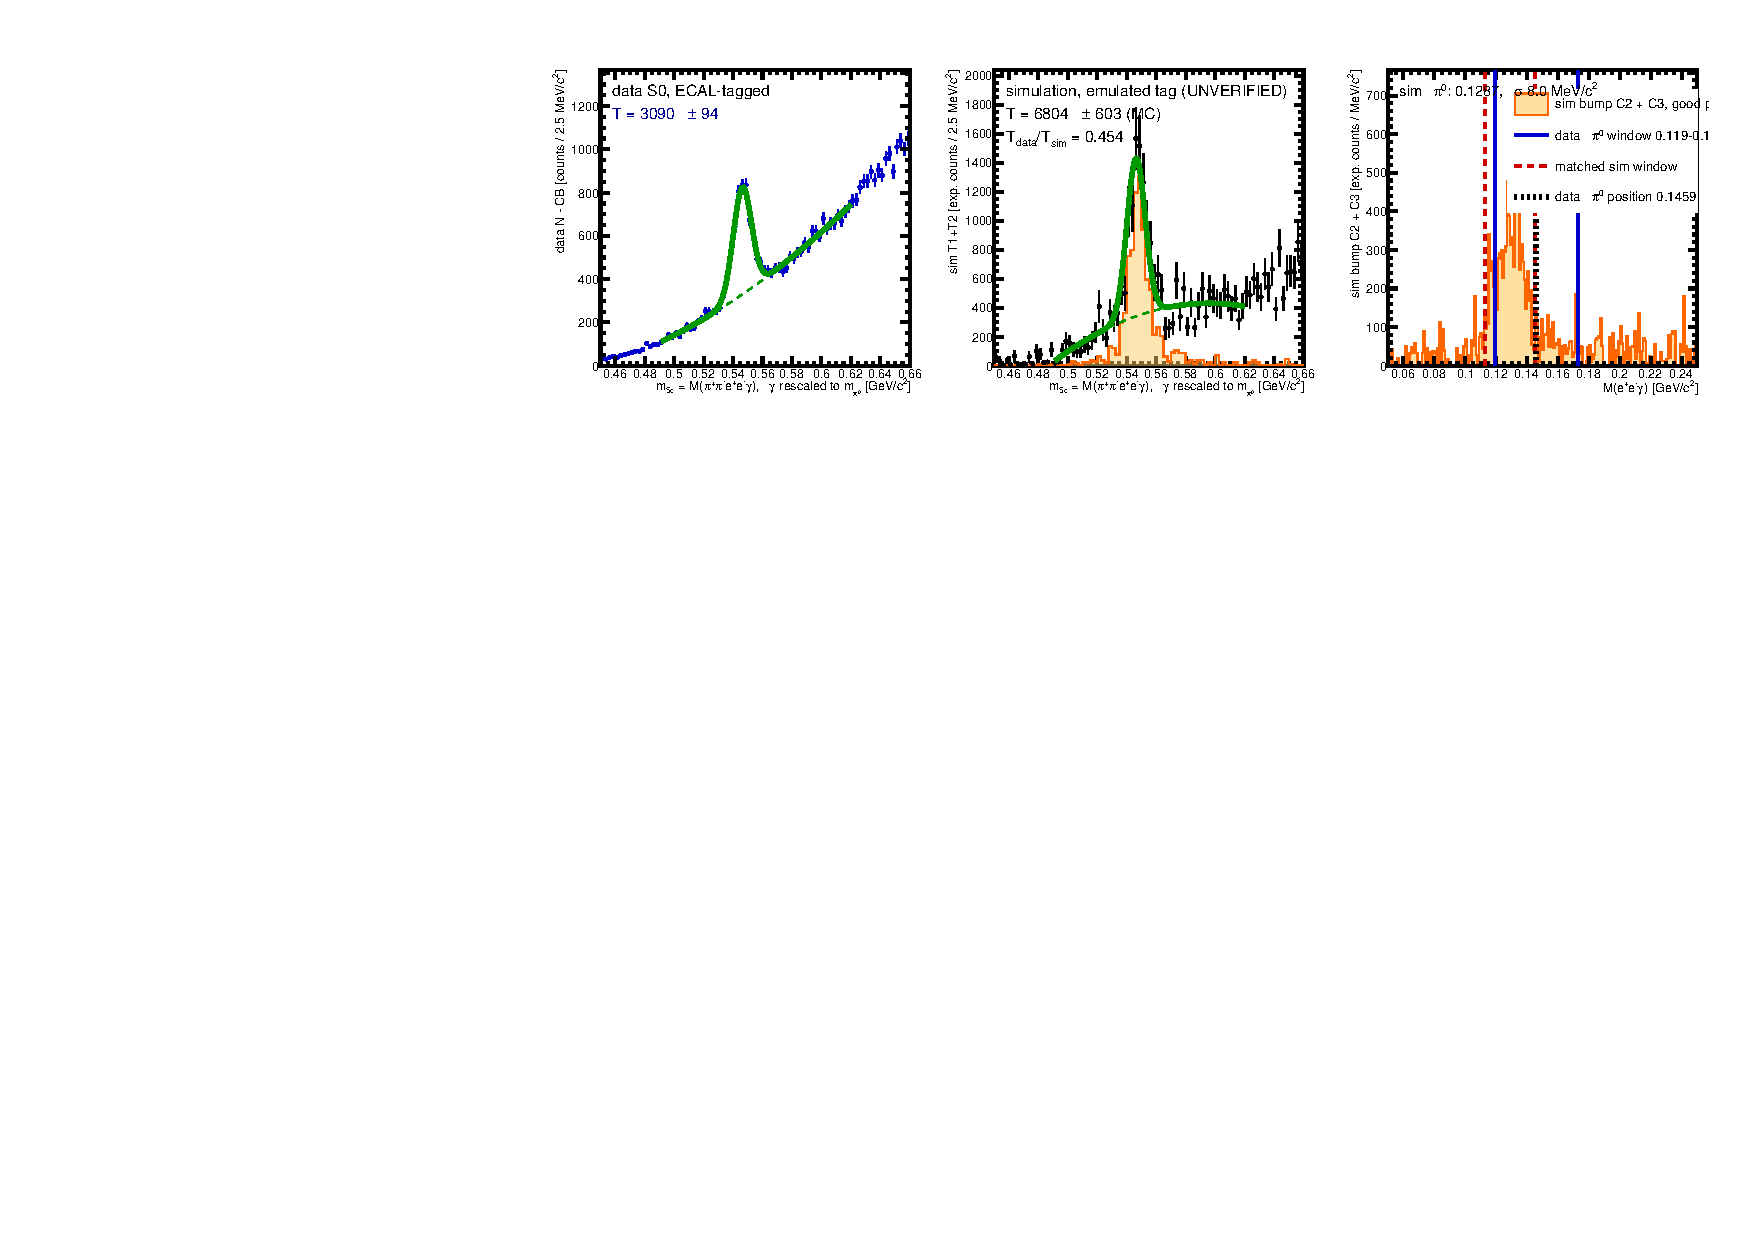
\includegraphics[width=\textwidth]{figs_all/wp6_tag_cnt.pdf}
\caption{ECAL tag.
Selection: (a) data, S0 (PT3 trigger, event vertex in the target region ($\vz>-160$\,mm), \betanew particle identification (pions within $3\sigma$, leptons within $5\sigma$ and with a RICH ring), energy-loss-corrected momenta of all four tracks, all stored combinations of each event (isBest $\ge0$), both pions in the event-vertex fit), all \Mfour and \Mpipi, counts with a good ECAL photon (photon identification, $0.8<\beta<1.2$, energy above 100\,MeV; of several the one with $M(\ee\gamma)$ closest to 0.140\,\GeVcc) with $0.119\le M(\ee\gamma)<0.173$\,\GeVcc and \Mee$<0.10$\,\GeVcc; m5c ($M(\pipi\ee\gamma)$, photon energy rescaled to $M(\ee\gamma)=m_{\piz}$) fitted in 0.49--0.62\,\GeVcc (CB in 20\,\MeVcc cells) with a fixed Gaussian (0.5463\,\GeVcc, 6.2\,\MeVcc) + pol2; ECAL sector 0 off in data and simulation. (b) $T_1+T_2$ of SMASH p+p at 4.5\,GeV (standard, lepton and $\eta$ sets, mode A) at its cross sections $\times$ PDG BR $\times$ the $\eta$-decay weights V3, masses moved to the data scale ($M_4'=0.99615\,M_4$, $\Mpipi'=0.9952\,\Mpipi$), same cuts, same photon selection and fit. (c) SMASH C2+C3 with S0, a good photon and \Mee$<0.10$\,\GeVcc, all \Mfour. (a) Data S0, ECAL-tagged counts: $N-\mathrm{CB}$ in m5c with the frozen fit (0.5463 / 6.2\,\MeVcc, pol2). (b) The emulated
simulated tag (acceptance verified in \S\ref{sec:ecalacc}; photon-energy scale not): $T_1+T_2$ with the same definition of a count; orange C2+C3. (c) Simulated $M(\ee\gamma)$ of the bump classes with a good
photon; blue: the data \piz window 0.119--0.173; red dashed: the window re-centred on the simulation; dotted: the data \piz position 0.1459. No fall-back involved.}
\label{fig:tag}
\end{figure}

%======================================================================
\section{Systematic uncertainties}
\label{sec:syst}
%======================================================================
\inshort{the peak yield carries 11.5\,\% systematic uncertainty (15\,\% with the specification's literal rules); \sigeta carries 36.6\,\%, mostly from the unknown make-up of the peak ($\pm31.8$\,\%; with the peak tail of D40, $\pm8.8$\,\%); the B4 bump area (157\,\%) and the double ratio derived from it (67\,\%) are not determined (the bump edge, with its own systematics, is in \S\ref{sec:bedge}).}
\notebox{\textbf{Result.} The peak is measured: \Ypeak carries 11.5\,\% systematic uncertainty with WP7's rules (15.2\,\% without rule R1,
14.7\,\% with the literal stat-only Barlow rule of the specification). \sigeta carries 36.6\,\%: 16.0\,\% from WP7, the composition of the
peak taken from the data ($\pm31.8$\,\%, review; the verifier v8 had used the prior $\kappa=1\pm0.2$, $\pm9.6$\,\%, total 18.5\,\%) and the
low-mass tail of the simulated peak ($\pm8.8$\,\%, D40; 35.5\,\% without it). Without
the composition the largest sources are the simulated peak resolution (S6), the side-band width (S2), the background model (S3), the
direct-decay weights (S7) and the displaced-window closure (S10). The absolute bump yield from B4 is \textbf{not determined} (157\,\%), and DR
inherits it (67\,\%); the bump edge has its own systematic families E1--E10 (8.9\,\% as is, 9.0\,\% C2 corrected, \S\ref{sec:bedge-syst}). The F-main and F-gold decompositions (\aEta, $Y_4$, $Y_5$, $\kappa$, \BRA, \BRG) are template- and model-limited at
50--130\,\%. The per-period stability test passes for every quantity. Table~\ref{tab:S1} and Fig.~\ref{fig:S1} include the S12 of WP8, the
composition term and the widened family S8 (review). The event-vertex efficiency, measured after the review, adds only a one-sided
$+2$\,\% ($+4$\,\% at 95\,\% CL) on the absolute scales, listed apart like the live time (\S\ref{sec:vertexeff}). The low-mass tail of the
simulated $\eta$ peak is a new family since D40 (approved by the analyst, option (a); \S\ref{sec:edgeu-tail}): it adds $\pm8.8$\,\% to \sigeta
(36.6\,\% instead of 35.5\,\%) and $\pm3.8$\,\% to \Ypeak (listed only, not counted); row S13 of Table~\ref{tab:S1}.}

\subsection{Procedure in plain words}
\begin{enumerate}\setlength{\itemsep}{0pt}
\item \textbf{Refit every variant.} For each variant of Sect.~5 of the specification (65 configurations) the whole chain is rerun: F-main
      $\to$ F-gold $\to$ stage A at the F-main $\eta$ values $\to$ B4 and the peak side bands. Ratios (DR, \BRG, \BRA) are recomputed inside each
      variant. For the control-region family (S2) only stage A and the estimators change. The generic code (\code{wp7_lib.h}) reproduces
      the nominal WP5 and WP6 numbers to all printed digits, and the fine layout G3 rebuilds the nominal to $10^{-7}$.
\item \textbf{Template noise of each variant difference.} For variants that use the nominal simulation in the standard layout, the whole
      chain is rerun with each of the 100 replicas; replica $r$ of the variant and of the nominal use the same simulated events, so the spread
      of their difference, MC($\Delta$) (half of the central 68\,\%), is the template noise of the variant shift. Other variants
      (other simulation samples, $s$/$r$ shifts, G3 layouts) get MC($\Delta$) $=0$ (conservative).
\item \textbf{Counting a variant.} $\Delta=$ variant $-$ nominal;
      $\delta^2=\max\big(0,\ \Delta^2-|\sigma_{\mathrm{stat},v}^2-\sigma_{\mathrm{stat},0}^2|-\mathrm{MC}(\Delta)^2\big)$ (Barlow subtraction of the
      statistical and of the template noise of the difference). A $\pm1\sigma$ pair counts $(|\Delta_+|+|\Delta_-|)/2$.
\item \textbf{Combining.} A family takes the largest $\delta$ of its variants; families add in quadrature; MC and the normalisation N are
      listed apart. Family S11 (selection) counts only for efficiency-corrected quantities and only if $|\Delta|>2\sqrt{|\sigma_v^2-\sigma_0^2|+
      \mathrm{MC}(\Delta)^2}$.
\item \textbf{Rule R1} (WP7 decision): a variant that the data reject is listed but not counted: same bins,
      $(\chi^2_v-\chi^2_0)/(\chi^2_0/\mathrm{ndf}_0)-(\mathrm{ndf}_0-\mathrm{ndf}_v)>25$; other bins, $(\chi^2_v/\mathrm{ndf}_v)/(\chi^2_0/\mathrm{ndf}_0)>1+5\sqrt{2/\mathrm{ndf}_v}$.
\end{enumerate}
\flag{The MC($\Delta$) subtraction and R1 are WP7 decisions taken after the variants were seen, not in the specification (D24, approved by the analyst on 15 November 2026); both lower the
totals.} \textbf{MC($\Delta$)}: without it a variant that changes how the noisy templates enter counts the template noise twice (example: raw
BB-lite templates move \Ypeak by $-451$ counts, but the replica spread of that difference is 1580 counts); the subtraction is the template-noise
analogue of the Barlow subtraction that the specification prescribes for the statistical noise. \textbf{R1} is a separate argument: a
variant that describes the data much worse than the nominal is not a plausible alternative model. Its threshold is relative (the
$\Delta\chi^2$ is divided by the nominal $\chi^2/\mathrm{ndf}$, so a mis-fitting nominal raises the threshold), but the nominal itself fails its
goodness of fit ($\chi^2/\mathrm{ndf}$ 2.6--3.4), and the threshold values (25 units; five standard deviations of the $\chi^2/\mathrm{ndf}$ ratio)
were chosen by WP7. The main item it removes is the $\omega$ split with the range to 0.85 ($+10.9$\,\% on \Ypeak). The totals as the
specification writes them (literal Barlow rule, no R1) are next to the nominal ones in Tables~\ref{tab:S1} and \ref{tab:alttot}: \Ypeak
14.7--15.2\,\% instead of 11.5\,\%, \sigeta 37.3--37.8\,\% instead of 36.6\,\% (with the peak tail of D40).

\begin{table}[H]
\centering
\caption{Spec.\ Table~S1: systematic uncertainties in per cent of the value. S0, isBest $\ge0$, $L=6079.2\,\nbinv$; yields in raw counts $\times64/63$.
Columns: \Ybump $=$ B4 (\Mee$\ge10$\,\MeVcc extrapolated to all \Mee; main bump estimator by fall-back, NOT DETERMINED); \Ypeak $=$ peak side
bands (MAIN); $Y_5$, $Y_4$ $=$ F-main C5/C4 in P; \aEta, \BRA $=\mathrm{BR}_{\mathrm{PDG}}\,\rhod$ and $\kappa$ from F-main; \BRG from F-gold
(CROSS-CHECKS, closure failed); DR $=\aP/a_B(\mathrm{all})$ (derived from B4, not determined); $\sigma_\eta=\aP\times1.0694$\,mb
$\times\Csec(1-\feta)$ (MAIN, PRELIMINARY). Values with PDG 2026. Families S1--S12 of the specification as combined by WP7, with three
updates of the review (in italics): S12 $=$ the completed S12 of WP8 (Table~\ref{tab:S12}) and, for $\sigma_\eta$, the composition of the peak
from the data ($\pm31.8$\,\%, \S\ref{sec:p2}); S8 widened to the observed range of $g$ (0.47--2.6) by linear extrapolation of WP7's ``$g$
free'' variant (\Ybump, \Ypeak, $Y_5$, $Y_4$, \aEta, $\sigma_\eta$; other columns as WP7). ``without rule R1'' and ``Barlow, stat only'': WP7's
alternative totals (recomputed for $\sigma_\eta$ only). MC and N separate; ``--'' in S11: not applied to raw yields. The X17 limit has its
own uncertainties inside the frozen likelihood (\S\ref{sec:x17}). Fall-backs: E1 and CR-K dropped, template fits demoted. Source: WP7
(\code{wp7_tableS1.txt}, \code{syst.txt}), updated by \code{fix_S1.py} (\code{tables_all/fix_tableS1.txt}). Last row (added with the vertex
study, \code{vtx_tableS1.tex}): the one-sided correction $C_{\mathrm{vtx}}$ of the event-vertex cut, $+2$\,\% ($+4$\,\% at 95\,\% CL) on the
absolute $\eta$ scales, 0 on the ratios (the bump keeps its vertex as the peak does), not applied and not in the total (\S\ref{sec:vertexeff}).
Final review (\code{fix2_tableS1.tex}): N of the absolute scales \aEta and $\sigma_\eta$ includes the $\pm5$\,\% period normalisation of Part~II.
Row S13 (fourth integration, \code{p3w_tableS1_v3.tex}): the family ``peak tail'' of D40 ($t=1\pm0.5$, approved by the analyst,
\S\ref{sec:edgeu-tail}), counted in the total of $\sigma_\eta$: $\pm8.8$\,\% (total 36.6\,\% instead of 35.5\,\%; without rule R1 37.8, Barlow
37.3); \Ypeak $\pm3.8$\,\% listed only (in parentheses, not in its total); last row: the totals before D40.}
\label{tab:S1}
\scriptsize
\setlength{\tabcolsep}{3pt}
\resizebox{\textwidth}{!}{\tabin{p3w_tableS1_v3.tex}}
\end{table}

\begin{figure}[H]
\centering
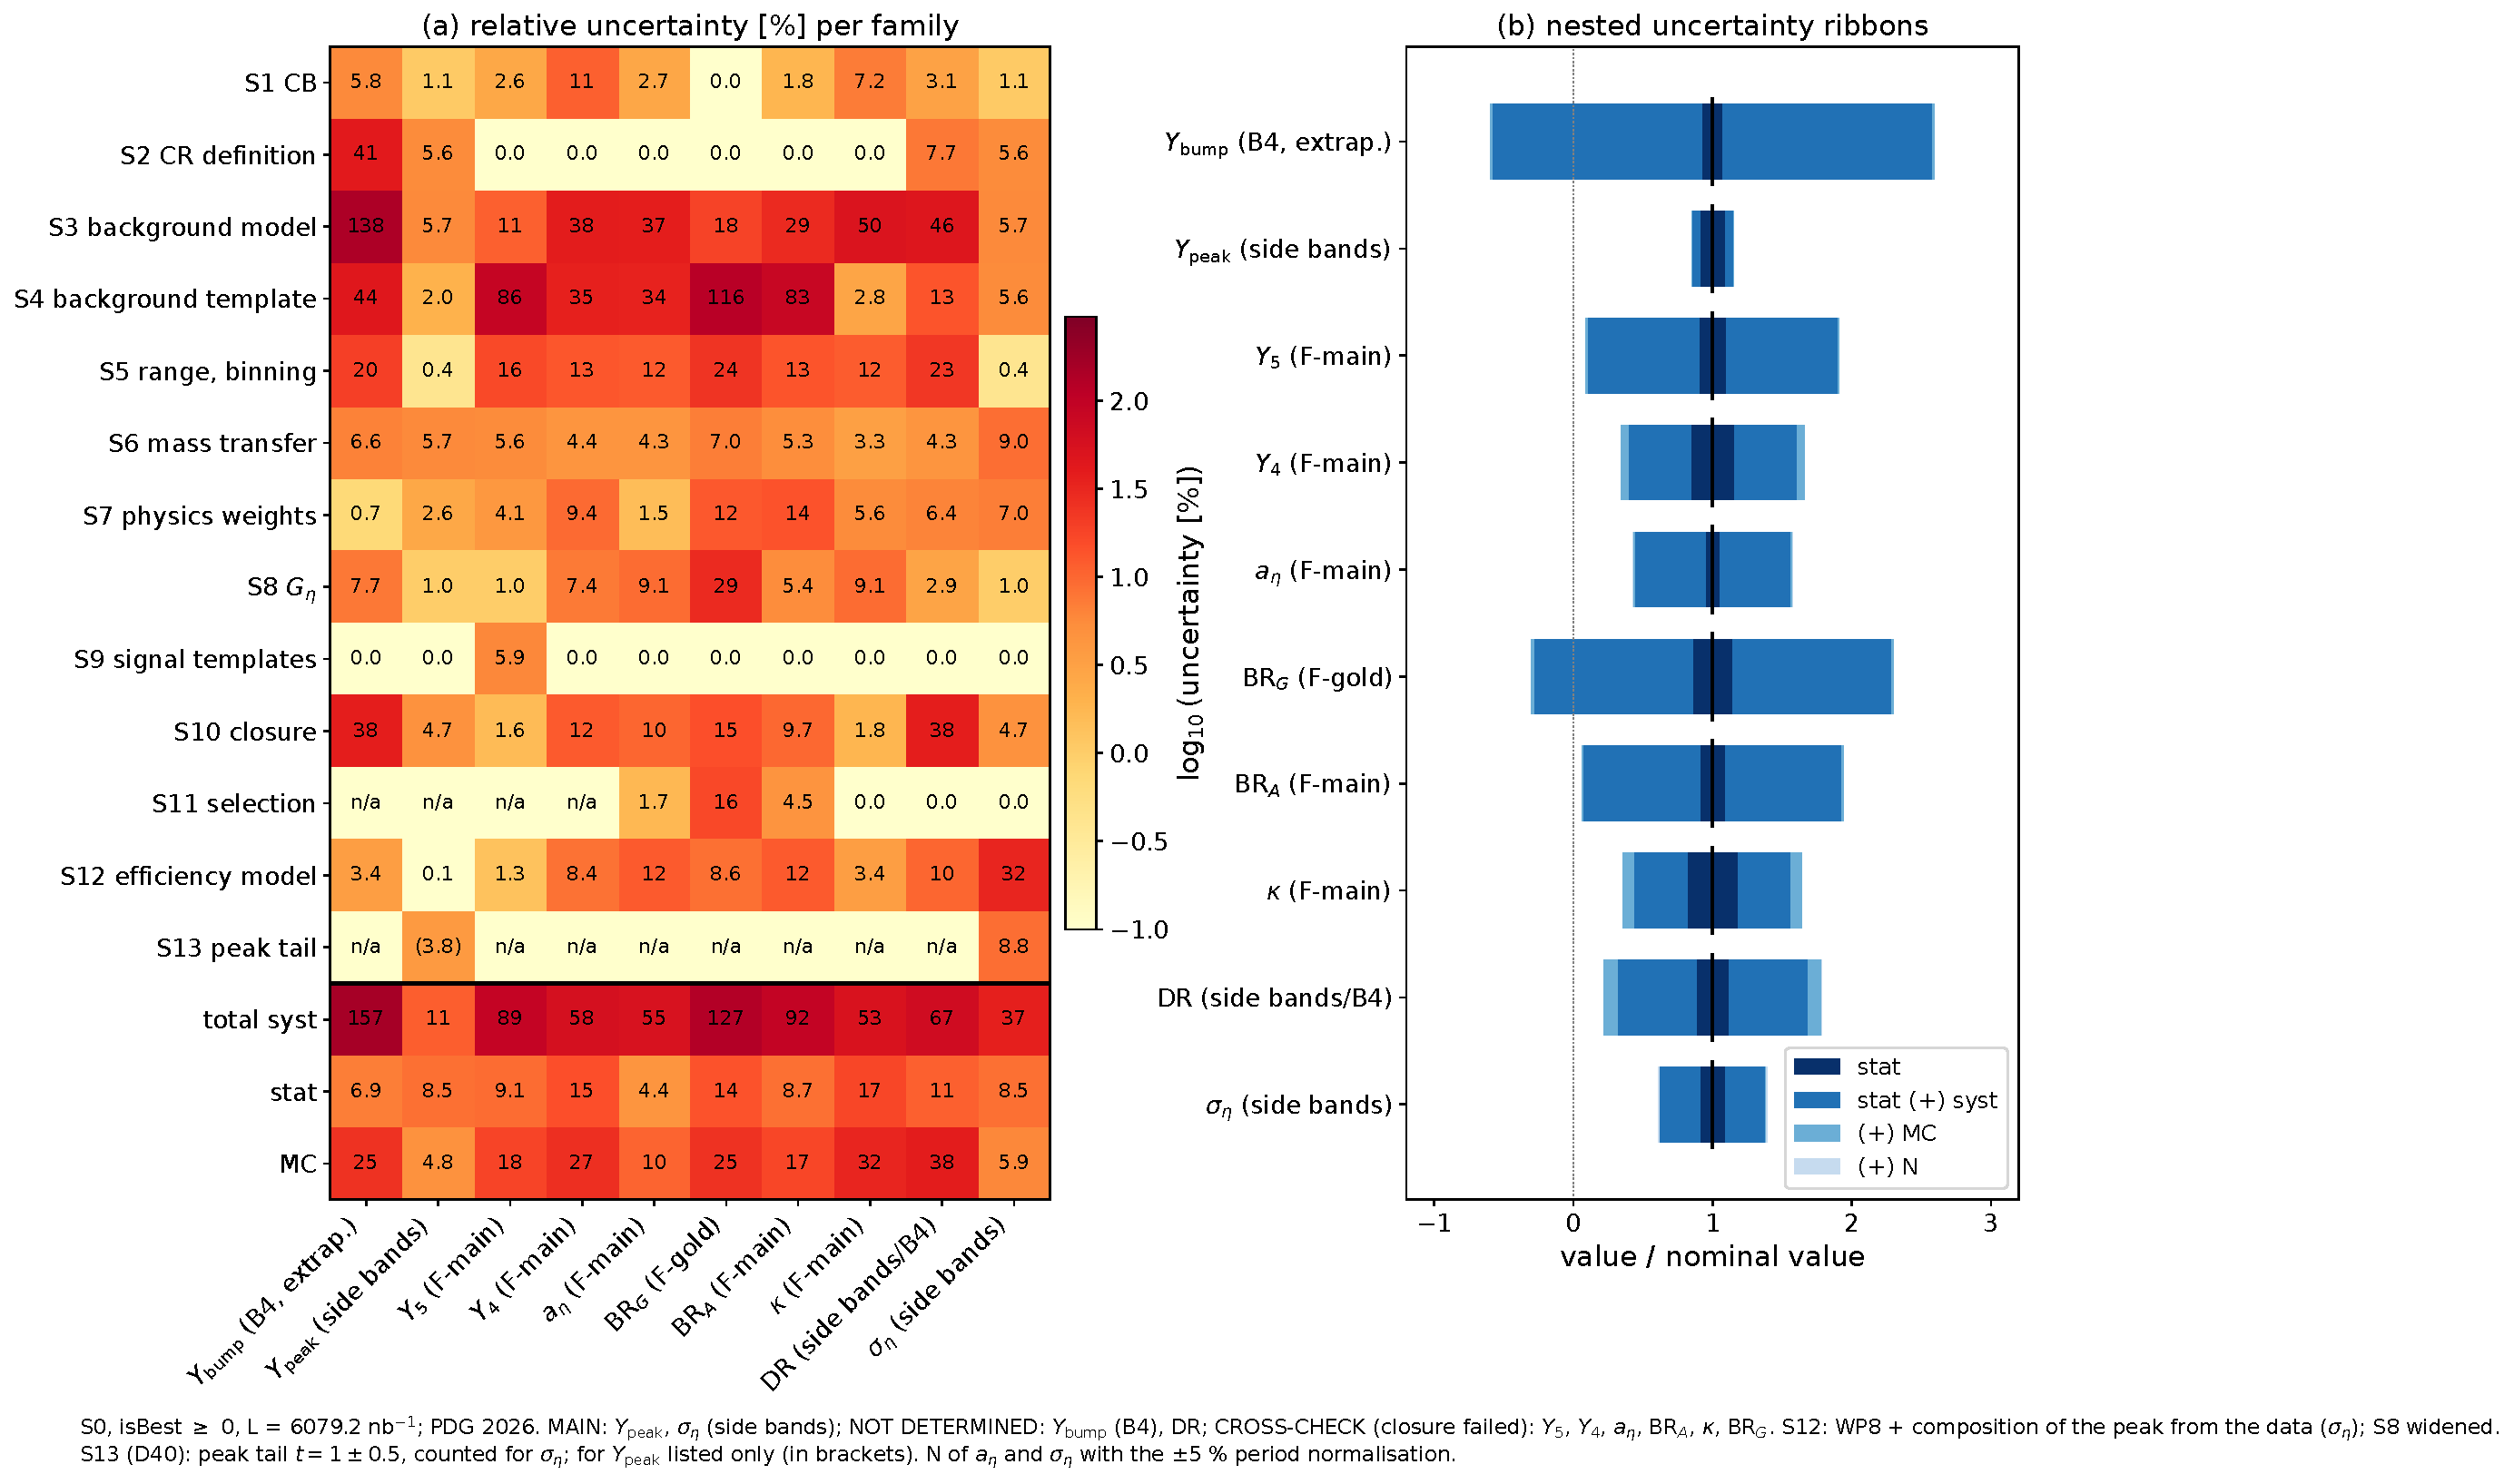
\includegraphics[width=\textwidth]{figs_all/fix_S1_v3.pdf}
\caption{Spec.\ Fig.~S1: systematic uncertainties of the Part~III quantities (Table~\ref{tab:S1}).
Selection: data, S0 (PT3 trigger, event vertex in the target region ($\vz>-160$\,mm), \betanew particle identification (pions within $3\sigma$, leptons within $5\sigma$ and with a RICH ring), energy-loss-corrected momenta of all four tracks, all stored combinations of each event (isBest $\ge0$), both pions in the event-vertex fit); CB $=2\sqrt{N_{++}N_{--}}$ of the like-sign data with the same cuts (10\,\MeVcc cells of \Mfour, $k=1$), shared out by the like-sign share of each 50\,\MeVcc band; SMASH p+p at 4.5\,GeV (standard, lepton and $\eta$ sets, mode A) at its cross sections $\times$ PDG BR $\times$ the $\eta$-decay weights V3, masses moved to the data scale ($M_4'=0.99615\,M_4$, $\Mpipi'=0.9952\,\Mpipi$), same cuts; each quantity with its own windows: \Ypeak, $\sigma_\eta$ from the peak window 0.53364--0.55416\,\GeVcc and side bands 0.5250--0.5336 and 0.5542--0.5628\,\GeVcc, all \Mee; \Ybump (B4), DR from the bump window 0.4550--0.5225\,\GeVcc, \Mee$\ge10$\,\MeVcc, background from \Mfour 0.575--0.700\,\GeVcc, extrapolated to all \Mee; template fits ($Y_5$, $Y_4$, \aEta, \BRA, $\kappa$) on \Mee$\ge10$\,\MeVcc, the \Mpipi slices $<0.34$, 0.34--0.37, 0.37--0.39, 0.39--0.43, $\ge0.43$\,\GeVcc, \Mfour 0.400--0.700\,\GeVcc; F-gold (\BRG) on \Mee$\ge20$\,\MeVcc. Data S0, isBest $\ge0$, $L=6079.2\,\nbinv$;
SMASH mode A, $w\times$V3, $M_4'=0.99615\,M_4$, PDG 2026. (a) Relative uncertainty in per cent per family S1--S13 (S13: the peak tail of D40, counted for $\sigma_\eta$; for \Ypeak listed only, in brackets) with the total systematic,
statistical and template-statistics (MC) errors; colour $=\log_{10}$ of the per-cent value. (b) Nested ribbons around value/nominal $=1$: stat,
stat $\oplus$ syst, $\oplus$ MC, $\oplus$ normalisation N (for \aEta and $\sigma_\eta$ with the $\pm5$\,\% period normalisation, as in Table~\ref{tab:S1}). MAIN: \Ypeak, $\sigma_\eta$ (side bands); NOT DETERMINED: \Ybump (B4), DR (from B4; the bump edge: \S\ref{sec:bedge});
CROSS-CHECK (closure failed): $Y_5$, $Y_4$, \aEta, \BRA, $\kappa$ (F-main), \BRG (F-gold). Family deltas after WP7's Barlow and MC($\Delta$)
subtraction; variants rejected by R1 not counted. S12 of WP8 and the composition of the peak included, S8 widened (review; redrawn by
\code{fix_S1.py} with WP7's plotting code; S13 and N by \code{fix_S1_v3.py}). The one-sided $C_{\mathrm{vtx}}$ row of Table~\ref{tab:S1} (added after the vertex study) is not drawn.}
\label{fig:S1}
\end{figure}

\begin{table}[H]
\centering
\caption{The dominant variants per quantity (shift of the variant; ``counted'' after the Barlow subtraction). Source: WP7
(\code{wp7_variants.txt}). Fall-backs: E1 dropped ($\kappa=1\pm0.2$); template fits demoted to cross-checks.}
\label{tab:domvar}
\small
\begin{tabular}{@{}p{2.0cm} p{13.4cm}@{}}
\toprule
quantity & dominant items \\
\midrule
\Ypeak & S3 D11data + $\omega$ split ($+6.6$\,\%, 5.7\,\% counted); S6 $r_{\mathrm{res}}=0.89/1.10$ ($-7.6/+4.7$\,\%); S2 wide/narrow side bands ($-6.7/-7.0$\,\%);
S7 conversion $F_V$ off ($+3.3$\,\%); S4 hybrid-GLS F-main ($+2.1$\,\%); S10 4.7\,\% \\
$\sigma_\eta$ & S6 $r_{\mathrm{res}}$ pair ($-10.8/+8.4$\,\%); S7 V2 ($-7.7$\,\%, the simulated C5 changes); S4 $w_{\mathrm{db}}$ ($-6.3$\,\%); S3 D11data + $\omega$
($+6.6$\,\%); S2 side-band width; S10 4.7\,\%; S12 2.5\,\% \\
\Ybump & S3 D11data ($+153$\,\%), quadratic ($+144$\,\%); S4 raw ($-49$\,\%), exp(pol4) ($-35$\,\%); S2 CR-U to 0.65 ($+47$\,\%); S5 \Mee split
8/12\,\MeVcc ($-16/-24$\,\%); S10 CR-L 37.5\,\% \\
DR & S3 D11data / quadratic (DR 0.58 / 0.60); S10 37.9\,\%; S5 \Mee split; S4 $w_{\mathrm{db}}$ (13\,\%) \\
\aEta & S3 quadratic ($+39$\,\%); S4 hybrid GLS ($+34$\,\%); S5 range 0.42--0.65 ($+15$\,\%); S10 10.1\,\% \\
\BRG & S4 raw BB-lite ($+121$\,\%); S8 $g$ free ($+32$\,\%); S5 range 0.45--0.70 ($-28$\,\%); S3 quadratic ($-25$\,\%); S11 $\dzpi<40$ ($+17$\,\%); S7 V2 ($-14$\,\%) \\
\BRA & S4 raw ($+87$\,\%); S3 quadratic ($-31$\,\%); S7 V2 ($-14$\,\%); S5 range 0.42--0.65 ($-17$\,\%) \\
$Y_5$ / $Y_4$ & S4 raw ($+89$\,\% / $+6$\,\%) and hybrid GLS ($+14$\,\% / $+38$\,\%); S3 $\kB=\kappa$ ($Y_4$ $+50$\,\%); S5 range; S1 per-cell geometric-mean CB ($Y_4$ $-12$\,\%) \\
$\kappa$ & S3 $\kB=\kappa$ (1.42); S5 slice edges; S8; S1 geometric-mean CB (0.76) \\
\bottomrule
\end{tabular}
\end{table}

\textbf{Variants rejected by the data (R1; listed, not counted).} Same bins: common $c\,(1+c_1y)$ (F-main 67, stage A 144 in units of the
threshold quantity); bump phase space instead of KLOE (F-main 38, F-gold 28); factorised signal templates (F-gold 71, \BRG only); $g=1\pm0.15$
(F-gold 28, \BRG only). Other bins: $\omega$ split with the range to 0.85 (F-main ratio 1.63 against the limit 1.32; stage A 1.55 vs 1.43;
\Ypeak shift $+10.9$\,\%); F-main range 0.40--0.75 (1.37 vs 1.36, marginal; \Ypeak $+2.0$\,\%).

\begin{table}[H]
\centering
\caption{Alternative totals of the systematic uncertainty (per cent): the literal Barlow rule with the statistical noise only, the total
without rule R1, and the sub-sources of S5/S6/S7 added in quadrature instead of the family maximum. WP7 values (S12 and S8 before the
updates of Table~\ref{tab:S1}); the $\sigma_\eta$ row ``with the composition'' recomputed with the composition term of the review and the
peak tail of D40 ($\pm8.8$\,\%). Source: WP7 (\code{syst.txt}),
\code{fix_numbers.txt}. Fall-backs: E1 dropped ($\kappa=1\pm0.2$); template fits demoted to cross-checks.}
\label{tab:alttot}
\small
\begin{tabular}{@{}>{\raggedright\arraybackslash}p{5.2cm} r r r r@{}}
\toprule
quantity & nominal & Barlow, stat only & without R1 & sub-sources in quadr. \\
\midrule
\Ybump & 157.2 & 171 & 157.5 & 157.4 \\
\Ypeak & 11.4 & 14.7 & 15.2 & 11.5 \\
$\sigma_\eta$ (WP7, without the composition) & 16.0 & 17.7 & 18.6 & 17.0 \\
$\sigma_\eta$ with the composition from the data (review) and the peak tail (D40) & 36.6 & 37.3 & 37.8 & 37.0 \\
DR & 66.3 & 118 & 67.7 & 66.7 \\
\aEta & 53.7 & 55.6 & 53.8 & 54.4 \\
\BRG & 126.6 & 132 & 144 & 126.6 \\
\bottomrule
\end{tabular}
\end{table}

\textbf{Further quantities} (value $\pm$ stat $\pm$ syst $\pm$ MC, WP7; PDG 2020): $\Ybump(E2)=7822\pm456\pm12\,870\,(165\,\%)\pm1920$;
$\aP=0.418\pm0.035\pm0.076\pm0.025$ (N 8.8\,\% with the $\pm5$\,\% period normalisation of Part~II, 7.3\,\% without; the syst here is WP7's
for $\sigma_\eta$, without the composition term, with the peak tail of D40: 16.0\,\% $\oplus$ 8.8\,\%; 0.153 with the composition term); $a_B(E2)=0.312\pm0.018\pm0.523\pm0.076$
($a_B(\mathrm{all})=0.299$); DR$_F$ (F-main) $=1.169\pm0.065\pm0.660\pm0.134$;
$\sigma_\eta$ from F-main $0.400\pm0.018\pm0.215\pm0.041$\,mb; $g=1.72\pm0.16\pm2.07\pm0.37$; $\rhod=1.32\pm0.12\pm1.20\pm0.23$. The F-main
statistical errors are not scaled; the $\chi^2$ rule of WP5 would multiply them by 1.38--1.61.

\textbf{Where WP7 deviated from the specification} (flagged): there is no V4 weight set (S7 uses V2 and GS); the eps2 QED check and the
$(p_T,y)$ reweighting of S12 were left to WP8 (\S\ref{sec:eff}); the \Mpipi scale $\pm0.0007$ was done by moving the simulated slice edges in G3
(effect $\le0.4$\,\%); ``$s$ free'' interpolates the $s$ shifts to the WP5 free values; in S1 ``\kEone free / 1'' and ``E1 dropped'' no longer
apply, ``1.032'' is CB$\times1.032$ with \kEtwo fixed, and ``like-sign sum'' is read as $N_{++}+N_{--}$; the CR-K variants are information
(CR-K rejected); the side-band widths come from WP6; S3 ``$\omega$ split, range 0.85'' is one variant (rejected by R1), the $\omega$ split on
the standard range is counted; S4 adds the hybrid-GLS F-main of v5 (not refitted by WP7); $\sigma_\eta$ comes from the side bands (\aP), not
from F-main.

\subsection{Family S12 completed (WP8) and the composition of the peak (v8)}
\begin{table}[H]
\centering
\caption{Family S12 (efficiency model) completed by WP8, per cent: pion-vertex efficiency (2.5\,\% on absolute scales, 2.0\,\% on ratios),
the QED $\gamma^*$ decay angle of class C2 (\S\ref{sec:eff}; sign known, not applied), the $3\times3$ $(p_T,y)$ reweighting (counted 0 after the
Barlow subtraction). S12 new $=$ maximum (the specification's family rule; quadrature changes the totals by $<0.1$ point). For
$\sigma_\eta$ the composition of the peak ($\pm31.8$\,\%) is added to S12 in Table~\ref{tab:S1}. Source: WP8 (\code{wp8_S12.txt}). No fall-back involved.}
\label{tab:S12}
\small
\begin{tabular}{@{}l r r r r r@{}}
\toprule
quantity & pion vertex & eps2 (angle) & $p_T/y$ $3\times3$ & S12 new & total syst old $\to$ new \\
\midrule
$\sigma_\eta$, \aP & 2.5 & 0.1 & 0 & 2.5 & $16.01\to16.01$ \\
\Ypeak & 0 & 0.1 & 0 & 0.1 & $11.43\to11.44$ \\
\aEta ($\sigma_\eta$ from F-main) & 2.5 & 12.2 & 0 & 12.2 & $53.7\to55.0$ \\
\BRG & 2.0 & 8.6 & 0 & 8.6 & $126.6\to126.9$ \\
\BRA, \rhod & 2.0 & 12.1 & 0 & 12.1 & $91.1\to91.9$ \\
DR & 2.0 & 10.2 & 0 & 10.2 & $66.3\to67.1$ \\
DR$_F$ & 2.0 & 7.0 & 0 & 7.0 & $56.4\to56.8$ \\
\aB & 2.5 & 12.4 & 0 & 12.4 & $167.8\to168.2$ \\
\Ybump & 0 & 3.4 & 0 & 3.4 & $157.2\to157.3$ \\
\bottomrule
\end{tabular}
\end{table}

\textbf{Composition of the peak} (verifier v8; taken from the data in the review). \aP $=\Ypeak/(\mathrm{C4}+\mathrm{C5})_{\mathrm{SMASH}}$ equals
the $\eta$ scale only if SMASH has the right mix of the conversion part C4 (47\,\% of the simulated peak) and the direct decays C5; no variant
of Table~\ref{tab:S1} moves it for the side-band estimator. The verifier v8 used the analysis' prior $\kappa=1\pm0.2$ ($\pm9.6$\,\%, total
18.5\,\%). That prior is a fall-back number, not a measurement, and three data indications point well below it: the side bands per \Mee class
($\kappa=0.37$), F-main on E1+E2 ($0.50\pm0.16$) and the X17 2D fit ($N_4/N_4^{\mathrm{ref}}$ against $N_5/N_5^{\mathrm{ref}}$: 0.51). The
composition systematic is therefore taken from the data (\S\ref{sec:p2}, \code{fix_numbers.py}): half the difference of the $\eta$ scale
from the direct decays alone (0.497) and from the conversions alone (0.237), relative to \aP (0.409, PDG 2026): $\pm31.8$\,\%. Added to S12 with
the family maximum it raises the systematic uncertainty of \sigeta from 16.0 to \textbf{35.5\,\%} (D31). DR is almost immune (1--3\,\%, C3 in
the bump moves the same way); \BRG is not affected (no C4 at \Mee$\ge20$\,\MeVcc).

\textbf{Family S8 widened} (review). The scale $g$ of \Geta is not robust: 1.72 in F-main, 2.19 in F-gold, 2.56 when free, 0.47--0.50 in the GLS
fits of the verifier v5. WP7's S8 varied only the width of the $g$ constraint and $g$ free (2.56). Extrapolating the ``$g$ free'' shift
linearly to $g=0.47$ (\code{fix_numbers.py}) gives \Ypeak $+1.0$\,\%, \Ybump $-7.7$\,\%, \aEta $+9.1$\,\%, $Y_4$ $-7.4$\,\%; these replace the
S8 entries where larger (Table~\ref{tab:S1}). The side bands depend on $g$ only through $R'$, so the peak result moves little; F-gold
(\BRG, S8 28.8\,\%) has $g$ free and is not extrapolated.

\subsection{Consistency tests}
\label{sec:periods}
\textbf{Per-period stability} (WP2 inputs; templates $\times L_p/L$ with $L_p=2809.453$ / 372.610 / 1078.022 / 1819.110\,\nbinv; factors
$K_p=\Csec(p)\times0.97$ with $\Csec(\mathrm{I})=1.0241\pm0.0077$ and 1 otherwise). The data errors of each period come from its own counts (event
groups and CB replicas); the stage-A, F-main and template errors are common to all periods and left out of the $\chi^2$.

\begin{table}[H]
\centering
\caption{Per-period stability test: \aEta (F-main type: background shape fixed, one free scale, $\kappa$ and $g$ fixed), \aP (peak side bands),
\aB (B4), DR$_F$ and DR per period; raw, $\times K_p=\Csec(p)(1-\feta)$, and $\times$ the old $K_p=\Csec(1-f_{\mathrm{win},p})$ (superseded by
Amendment~1, IIA--IIB correlated); $\chi^2$ against the weighted mean. All pass ($p>0.01$). Source: WP7 (\code{wp7_periods.txt}). Fall-backs: E1 dropped ($\kappa=1\pm0.2$); template fits demoted to cross-checks.}
\label{tab:periods}
\small
\resizebox{\textwidth}{!}{\tabin{fix_periods.tex}}
\end{table}

Period IIA (6\,\% of $L$) is high in \aB ($+2.2\sigma$) and low in DR$_F$ ($-2.3\sigma$); neither reaches $p<0.01$. The F-main-type values
agree with WP5 (0.36684 / 0.42339 / 0.38319 / 0.36782); the small differences come from the analysed-run luminosity shares and the periods' own
CB replicas.

\textbf{Folds} (event-group parity): no quantity has $p<0.05$ (largest: \Ypeak(F-main) $z=-1.55$; \Ypeak, \aP, $\sigma_\eta$ $z=-1.43$ with
fold0 $4479\pm611$, fold1 $5713\pm610$; \aEta $z=-1.37$); no fold term is added. \textbf{isBest $=1$ / isBest $\ge0$} (data only, same isBest
$\ge0$ templates, independent-sample bound for stat): \Ypeak $0.915\pm0.109$, \Ybump $0.885\pm0.087$, \aEta $0.867\pm0.055$, DR $1.03\pm0.16$,
\BRG $1.05\pm0.21$, \BRA $1.04\pm0.13$. \textbf{\code{cor_ok} fall-back} (nested sample; not combined): the ratios are unchanged (DR $z=-0.06$,
\BRG $+0.18$, \BRA $+0.44$); yields and absolute scales rise by about 2.2\,\% (\Ypeak $+111$ counts, $z=+2.3$; \aEta $z=+2.2$; \aB $z=+3.2$), as
expected: the fall-back adds about 1.3\,\% \ee counts (P: 56\,672 vs 55\,947), and the simulation has no \code{cor_ok} $=0$ entries.

%======================================================================
\section{Physics results}
\label{sec:phys}
%======================================================================
\inshort{$\sigeta=0.429\pm0.036\pm0.157\pm0.025\,^{+0.041}_{-0.043}$\,mb (PRELIMINARY, D28), with a separate production-model item
$^{+0.08}_{-0.03}$\,mb (D29), 0.40 of SMASH and 0.38--0.46 of the HADES values at 3.5\,GeV. The event-vertex cut keeps $0.994\pm0.021$ of the $\eta$ and is not the cause of the low value; the target walls carry only $3^{+4}_{-3}$\,\% of the $\eta$ (applied, D21, approved); HGeant's isotropic $\gamma^*$ decay makes the simulated efficiency of the bump counts about 16\,\% too high (12--14\,\% in the toys and the closure; corrected with per-count weights at the bump edges, D38).}
\subsection{Normalisation items: sector-2 deficit and target material}
\label{sec:norm}
\textbf{What $L$ contains} (luminosity files and the Task~E documents of the luminosity analysis): the PT2 live fraction and duty factor;
the sector-2 PT2 (elastic) deficit of days 034--044, removed by replacing sector 2 with $\rho\times$ the mean of the other sectors
(factor 1.058--1.120 per day; day 045 has none in the elastic events, see the PT2 check below); and the removal of the elastic events from the target windows ($w_6=0.702$ / 0.806 / 0.806 / 0.883\,\% in
I / IIA / IIB / III). $L$ does \emph{not} contain 64/63, the PT3 live fraction (D17), the sector-2 deficit of the PT3 channel counts
(\Csec) and the material contribution to the channel counts (\fwin); the luminosity file says so verbatim (``Sector 2 on days 034--044 has
a hardware trigger deficit that is NOT in L'', ``Yields must be empty-target subtracted (L is LH2 only)'').

\textbf{Sector-2 deficit of the channel, \Csec} (WP2). Procedure:
\begin{enumerate}\setlength{\itemsep}{0pt}
\item Sector number $=(\lfloor\varphi/60^\circ\rfloor+5)\bmod 6$; verified on the acceptance gaps of the S0 lepton tracks (content within
      $\pm1^\circ$ of the six boundaries / side bands $=0.001$) and by the rate deficit of the early days, which lies exactly in
      180--240$^\circ$ (Fig.~\ref{fig:N1}a).
\item The efficiency $\varepsilon_{s2}$ is a double ratio: counts that use a sector-2 track against counts that do not, deficit days against clean
      days (this removes $L$ and global drifts). In blocks of 25\,\nbinv (Fig.~\ref{fig:N1}b) the deficit is intermittent: 30 blocks of days
      034--045 lie more than $4\sigma$ below 1 (down to 0.58), one block elsewhere (day 061). Day 045 still has three deficit blocks (day
      $\varepsilon=0.903\pm0.007$), day 046 none ($1.008\pm0.007$). \flag{Deviation: the nominal deficit span is 034--045, not the 034--044
      of the specification and of the elastic analysis; the specification span is a variant. Approved by the analyst on 15 November 2026
      (D26).} $\varepsilon_{s2}=0.9266\pm0.0024$ (034--045
      vs 046--067).
\item The share $f_s$ of the signal with a sector-2 track comes from the simulation (S0, V3, mode A): bump C2+C3 in B $0.326\pm0.012$,
      peak C4+C5 in P $0.362\pm0.016$.
\item $\Csec=1/[1-f_s(1-\varepsilon_{s2})\,L_{034-045}/L]$ (exact form; the first-order form of the specification is 0.07\,\% higher).
      Systematics: the loss per sector pattern or per number of sector-2 tracks, $f_s$ from the clean-day data, the span 034--044.
\end{enumerate}
Result: $\Csec=1.0104\pm0.0005\pm0.0035$ (bump), $1.0116\pm0.0006\pm0.0029$ (peak), mean for the $\eta$ $1.0110\pm0.0035$; period I alone
1.0229 / 1.0254. The ratios peak/bump (1.0011) and C5/C2 (1.0020) are 1 within 0.2\,\%, so no correction is needed for DR and \BRG.
Indicative check: $\aEta(\mathrm{IIA+IIB+III})=0.380\pm0.011$ against $\aEta(\mathrm{I})\times\Csec(\mathrm{I})=0.376\pm0.013$.

\textbf{Sector 2 in the elastic events: the PT2 check (D26).} In short: on day 045 the elastic events have no sector-2 deficit, so the
luminosity is right and only the lepton channel is low. The analyst's luminosity table (\code{s2_trigger_perday.csv}: elastic events per sector
and day, for PT2 and PT3) gives, per day, sector 2 relative to the mean of the other sectors, divided by the same ratio on the clean days 046--067
(1 = no deficit; data only):
\begin{center}\small
\begin{tabular}{@{}l c c c c c c c@{}}
\toprule
day & 041 & 042 & 043 & 044 & 045 & 046 & 047 \\
\midrule
PT2 & $0.654\pm0.006$ & 0.762 & 0.688 & 0.753 & $1.074\pm0.009$ & 1.087 & 1.005 \\
PT3 & $0.915\pm0.007$ & 0.981 & 0.941 & 0.983 & $1.074\pm0.008$ & 1.098 & 1.010 \\
\bottomrule
\end{tabular}
\end{center}
On days 041--044 the elastic events lose 24--35\,\% of their sector-2 PT2 triggers (2--9\,\% in PT3); on day 045 they lose none, in PT2 or PT3. The
luminosity, which replaces the sector-2 PT2 rate only on 034--044, is therefore right on day 045, and $L=6079.2\,\nbinv$ is unchanged. The deficit
of the \ppee counts on day 045 (sector-2 efficiency $0.903\pm0.007$; deficit periods 0:00--2:07, 2:08--4:05 and 7:27--17:56) is specific to the
lepton channel; its cause was not studied. \Csec keeps the span 034--045, approved by the analyst on 15 November 2026 (D26).

\textbf{Target material, \fwin} (WP2). Empty-target DSTs exist for the days 034 (7 runs), 047 (16) and 065 (104): 127 runs, 1270 DSTs,
the same days the luminosity analysis used. Procedure:
\begin{enumerate}\setlength{\itemsep}{0pt}
\item PAT was rebuilt from the production tag (sources identical, same PID file) and run on vae25 (44 jobs, all successful; one
      full-target DST gives identical entries to the production); FAT with the data configuration ($T=4530$, PT3, corrected momenta); compact
      file with a copy of the data \code{scan_prepare.C} (paths only changed).
\item \textbf{Flux normaliser} $b$ (full/empty, same day): the channel counts (isBest $\ge0$, $\vz>-500$, PT3, \code{cor_ok}; us + pp + mm) with
      \vz in $[-200,-170)$\,mm, where the beam hits the material in front of the cell in both kinds of runs and the simulated LH$_2$ puts only
      $1.7\times10^{-5}$ of its entries: $b=10.35\pm0.79$ (034), $15.44\pm0.95$ (047), $0.932\pm0.030$ (065). A vz-profile fit (LH$_2$ simulation +
      empty target) gives 0.85--0.90 of these values (lower bound); positivity of full $-$ $b\times$empty in the entrance-window bin gives an upper
      bound 1.06--1.22 $\times\,b$. Normalisers built from \ee counts violate the positivity bound and are rejected.
\item $\fwin=b\,Y_{\mathrm{empty}}/Y_{\mathrm{full}}$ per selection, window and quantity, combined over the days with the luminosity of the
      period each day represents (034 $\to$ I, 047 $\to$ IIA + IIB, 065 $\to$ III).
\end{enumerate}
Results ($N-\mathrm{CB}$, S0): all \Mfour $11.86\pm0.59$\,\%, B $18.64\pm2.04$\,\%, P $15.78\pm3.07$\,\%, B+P $16.76\pm1.88$\,\%, 0.40--0.70
$13.12\pm0.85$\,\%, CR-U $12.29\pm0.87$\,\%; ``pre'' (B+P) 22.44\,\%, $\vz>-150$ 12.36\,\%, $\vz>-170$ 19.00\,\%; like-sign counts $29.7\pm2.2$\,\%.
The material spectrum is softer: \fwin is 0.11--0.12 above 0.56\,\GeVcc and 0.15--0.25 below 0.52 (Fig.~\ref{fig:N1e}). The material share
is physical: the gen4 target (LH$_2$ cell $-148.4$ to $-98.6$\,mm, three Mylar windows of 0.1\,mm) has 0.3\,mm Mylar $=11.9$\,\% of the LH$_2$
nucleons, i.e.\ 5--12\,\% with an $A^{2/3}$--$A^1$ scaling; the design expectation of 0.7--2.1\,\% scaled the elastic window share of free
protons only.

\notebox{\textbf{Amendment~1 (verification of WP2, binding; approved by the analyst on 15 November 2026, D21).} Two independent verifiers reproduced every WP2 number but showed that the
$\eta$ \emph{signal} has almost no material component: in vertex slices of the full data the cell-centre method gives $\feta=1.5\pm4.5$\,\%,
shape fits 0.0--2.7\,\%; in the slice $-160$ to $-150$\,mm (71--83\,\% material counts) the tagged $\eta$ is 2.9\,\% of $T$ against 2.4--2.8\,\%
from the LH$_2$ simulation tail; the share of $S$ and $T$ in the cell centre ($0.566\pm0.045$, $0.571\pm0.024$) matches the simulation (0.577)
and excludes a 16.8\,\% material share (0.497) at 3.4$\sigma$. Decision: $\feta=3^{+4}_{-3}$\,\%, and every $\eta$ yield, BR or cross section
uses $\Csec\times(1-\feta)=0.98^{+0.03}_{-0.04}$ ($1.011\times0.97$ with the mean \Csec of bump and peak; \sigeta uses \Csec of the peak,
$1.0116\times0.97=0.981$), never $1-\fwin$. [Reason as corrected in the review: the side bands and the
background model remove the non-peaking material counts in any case; \fwin measures the material share of \emph{all} $N-\mathrm{CB}$ counts,
which is dominated by the non-$\eta$ background, so it does not describe the $\eta$ signal. The amendment's wording ``would remove the
material twice'' is not the reason.] \fwin describes only the composition of the non-$\eta$ background: about
13--15\,\% of $N-\mathrm{CB}$ in 0.40--0.70 is material that SMASH does not simulate. The halo normaliser is not representative of the periods
(the halo-to-core ratio varies by 19\,\% rms); reweighted, $\fwin(\mathrm{B+P})=14.7\pm1.1\,(\mathrm{stat})^{+1.0}_{-2.0}\,(\mathrm{syst})$\,\%
(all \Mfour $11.3\pm0.4^{+0.8}_{-1.5}$\,\%); the gas term of WP2 ($-3.6$\,\%) is too large (at most about 1\,\%). Per-period factors:
$K_p=\Csec(p)\times0.97$.}

\textbf{Coverage of $\feta$ (review).} The nucleon-count expectation for $\eta$ produced in the Mylar windows is 5--12\,\% (above); the
adopted $\feta=3^{+4}_{-3}$\,\% covers its lower half only. The measurement behind the amendment (cell-centre share $0.566\pm0.045$ against
0.577 in the LH$_2$ simulation; vertex slices $\feta=1.5\pm4.5$\,\%) puts 12\,\% at about $2.3\sigma$, so the binding value is
kept and not widened. The upper end is quoted as a known-sign item: with $\feta=12$\,\% \sigeta would be
9\,\% lower (0.389\,mb; \S\ref{sec:p2}).

\begin{table}[H]
\centering
\caption{Spec.\ Table~N1: normalisation items for absolute quantities. $L$: START-free elastic luminosity of the analysed runs (LH$_2$ only, with
the sector-2 PT2 removal and $w_6$). \Csec: sector-2 PT3 deficit of days 034--045 for the channel counts. \fwin: material share of
$N-\mathrm{CB}$ (S0, isBest $\ge0$) from the empty-target runs of days 034, 047, 065. \feta: material share of the $\eta$ signal
(Amendment~1); \sigeta uses \Csec of the peak (1.0116; the mean of bump and peak is 1.0110). Period normalisation: the $\pm5$\,\% of Part~II for
the steps of the per-day rates between the beam periods (cause not proven; Part~II: they follow the beam-halo level, an indication). Sources: WP2 (\code{wp2_N1.txt}) and its verification (\code{docs/latex/notes_all/verify_wp2/}). \flag{The WP2 rows ``\fwin recommended for $\eta$
$16.8^{+5.0}_{-5.9}$\,\%'' and ``$\Csec(1-\fwin)=0.842$'' of \code{wp2_N1.tex} are superseded by Amendment~1.} No fall-back involved.}
\label{tab:N1}
\footnotesize
\begin{tabular}{@{}l l r@{}}
\toprule
item & selection / window & value \\
\midrule
$L$ [\nbinv] & all / I / IIA / IIB / III & 6079.2 / 2809.5 / 372.6 / 1078.0 / 1819.1 \\
$L$ [\nbinv] & deficit days 034--045 / clean 046--067 & 2619.6 / 3459.6 \\
period normalisation & integrated yields per $L$ (Part~II) & $\pm5$\,\% (in N of \sigeta) \\
$\varepsilon_{s2}$ & counts with a sector-2 track, 034--045 & $0.9266\pm0.0024$ \\
$f_s$ (simulation) & bump C2+C3 / peak C4+C5 & 0.326 / 0.362 \\
\Csec & bump C2+C3 in B / peak C4+C5 in P & $1.0104\pm0.0035$ / $1.0116\pm0.0030$ \\
\Csec & period I only (bump / peak) & 1.0229 / 1.0254 \\
\midrule
\fwin [\%] & all \Mfour / B / P / B+P & $11.9\pm0.6$ / $18.6\pm2.0$ / $15.8\pm3.1$ / $16.8\pm1.9$ \\
\fwin [\%] & 0.40--0.70 / CR-U & $13.1\pm0.9$ / $12.3\pm0.9$ \\
\fwin [\%] & B+P, halo-reweighted (verification) & $14.7\pm1.1^{+1.0}_{-2.0}$ \\
\midrule
\feta [\%] & $\eta$ signal (Amendment~1) & $3^{+4}_{-3}$ \\
$\Csec(1-\feta)$ & every $\eta$ yield, \sigeta & $0.98^{+0.03}_{-0.04}$ (\sigeta: $1.0116\times0.97=0.981$) \\
$(1-f_P)/(1-f_B)$ & ratios (information; not applied) & $1.035\pm0.046$ \\
\midrule
$\varepsilon_{\mathrm{vtx}}(\eta)$ (\S\ref{sec:vertexeff}) & $\vz>-500$\,mm, data / simulation & $0.994\pm0.021$ / 0.9997 \\
$C_{\mathrm{vtx}}$ (not applied) & \sigeta / bump scale & $1.006\pm0.021$ / $1.00\pm0.02$ \\
\bottomrule
\end{tabular}
\end{table}

\begin{figure}[H]
\centering
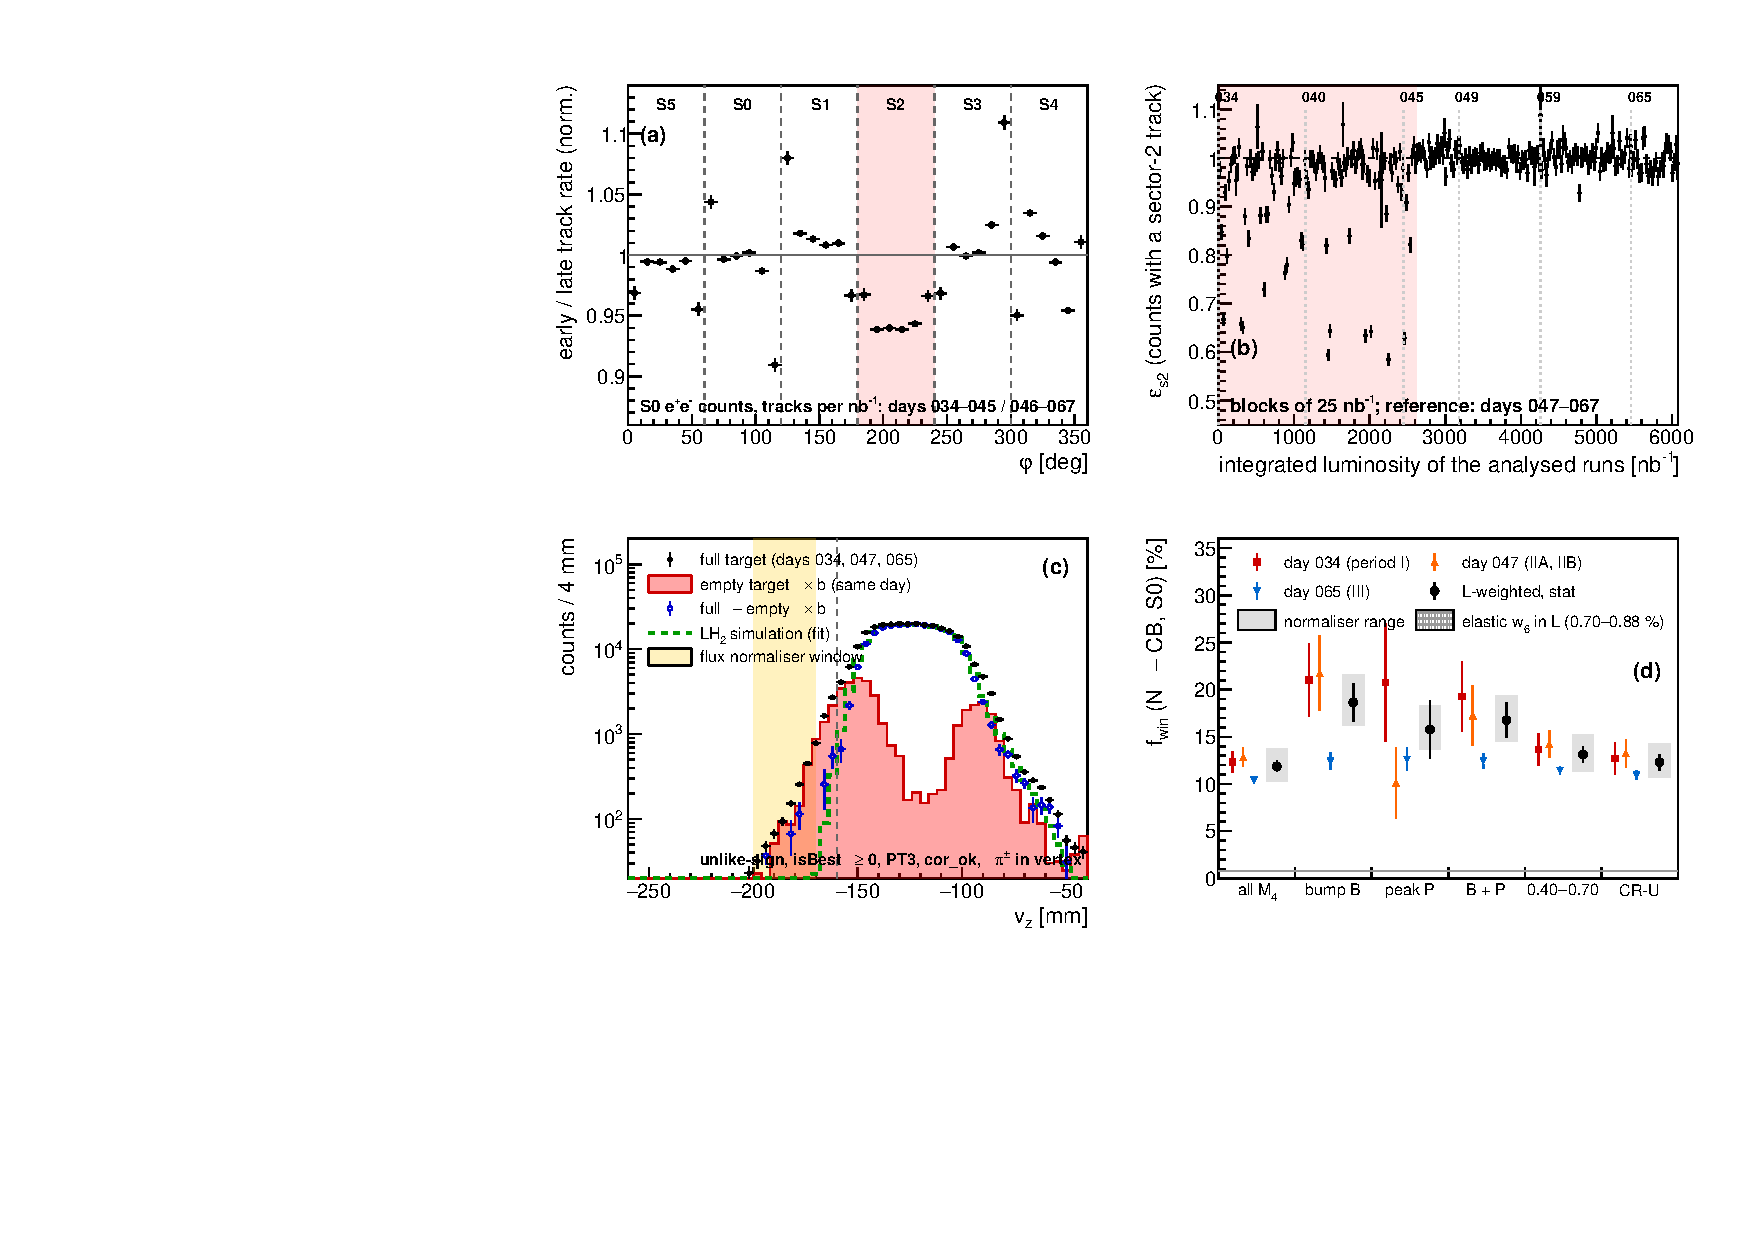
\includegraphics[width=0.9\textwidth]{figs_all/wp2_N1v2_cnt.pdf}
\caption{Spec.\ Fig.~N1: normalisation items.
Selection: data. (a) all four tracks of the unlike-sign S0 counts (PT3 trigger, event vertex in the target region ($\vz>-160$\,mm), \betanew particle identification (pions within $3\sigma$, leptons within $5\sigma$ and with a RICH ring), energy-loss-corrected momenta of all four tracks, all stored combinations of each event (isBest $\ge0$), both pions in the event-vertex fit), all \Mfour, per 10$^\circ$ of azimuth, days 034--045 against 046--067. (b) unlike-sign S0 counts, all \Mfour, with a track in sector 2 (azimuth 180--240$^\circ$) against those without, per block of 25\,\nbinv, reference days 047--067. (c) the same cuts without $\vz>-160$\,mm (event vertex $\vz>-500$\,mm with both pions in its fit), all \Mfour, days 034, 047, 065, full and empty target; flux ratio $b$ from all three hypotheses in $-200\le\vz<-170$\,mm. (d) $N-\mathrm{CB}$ of S0 in \Mfour windows: all, 0.4550--0.5225, 0.53364--0.55416, both, 0.40--0.70, 0.565--0.700\,\GeVcc; CB $=2\sqrt{N_{++}N_{--}}$ of each window. (a) Track rate per \nbinv of the S0 \ee counts (isBest $\ge0$), days 034--045 / days 046--067, per
10$^\circ$ of azimuth, normalised outside 180--240$^\circ$; the labels S0--S5 are the \emph{sector} numbers. The deficit is confined to
sector 2. (b) $\varepsilon_{s2}$: counts with a sector-2 track relative to counts without one, per block of 25\,\nbinv of the analysed runs,
normalised to days 047--067; shaded: the deficit span 034--045. (c) Vertex $z$ of the unlike-sign combinations (isBest $\ge0$, PT3, \code{cor_ok},
both pions in the vertex fit, all \Mfour), days 034 + 047 + 065: full target (black), empty target $\times\,b$ (red; flux ratio of the same day
from the counts in the shaded window $-200$ to $-170$\,mm), their difference (blue), LH$_2$ simulation fitted to the full-target profile (green);
dashed: the cut $\vz>-160$\,mm. (d) \fwin, the material share of $N-\mathrm{CB}$ in S0 per \Mfour window, per empty-target day and
$L$-weighted (statistical errors); grey boxes: range of the flux ratio (vz-profile fit to positivity bound); hatched: the elastic window
fraction $w_6$ already removed from $L$. $L=6079.2\,\nbinv$. By Amendment~1, \fwin is \emph{not} applied to $\eta$ yields. No fall-back involved.}
\label{fig:N1}
\end{figure}

\begin{figure}[H]
\centering
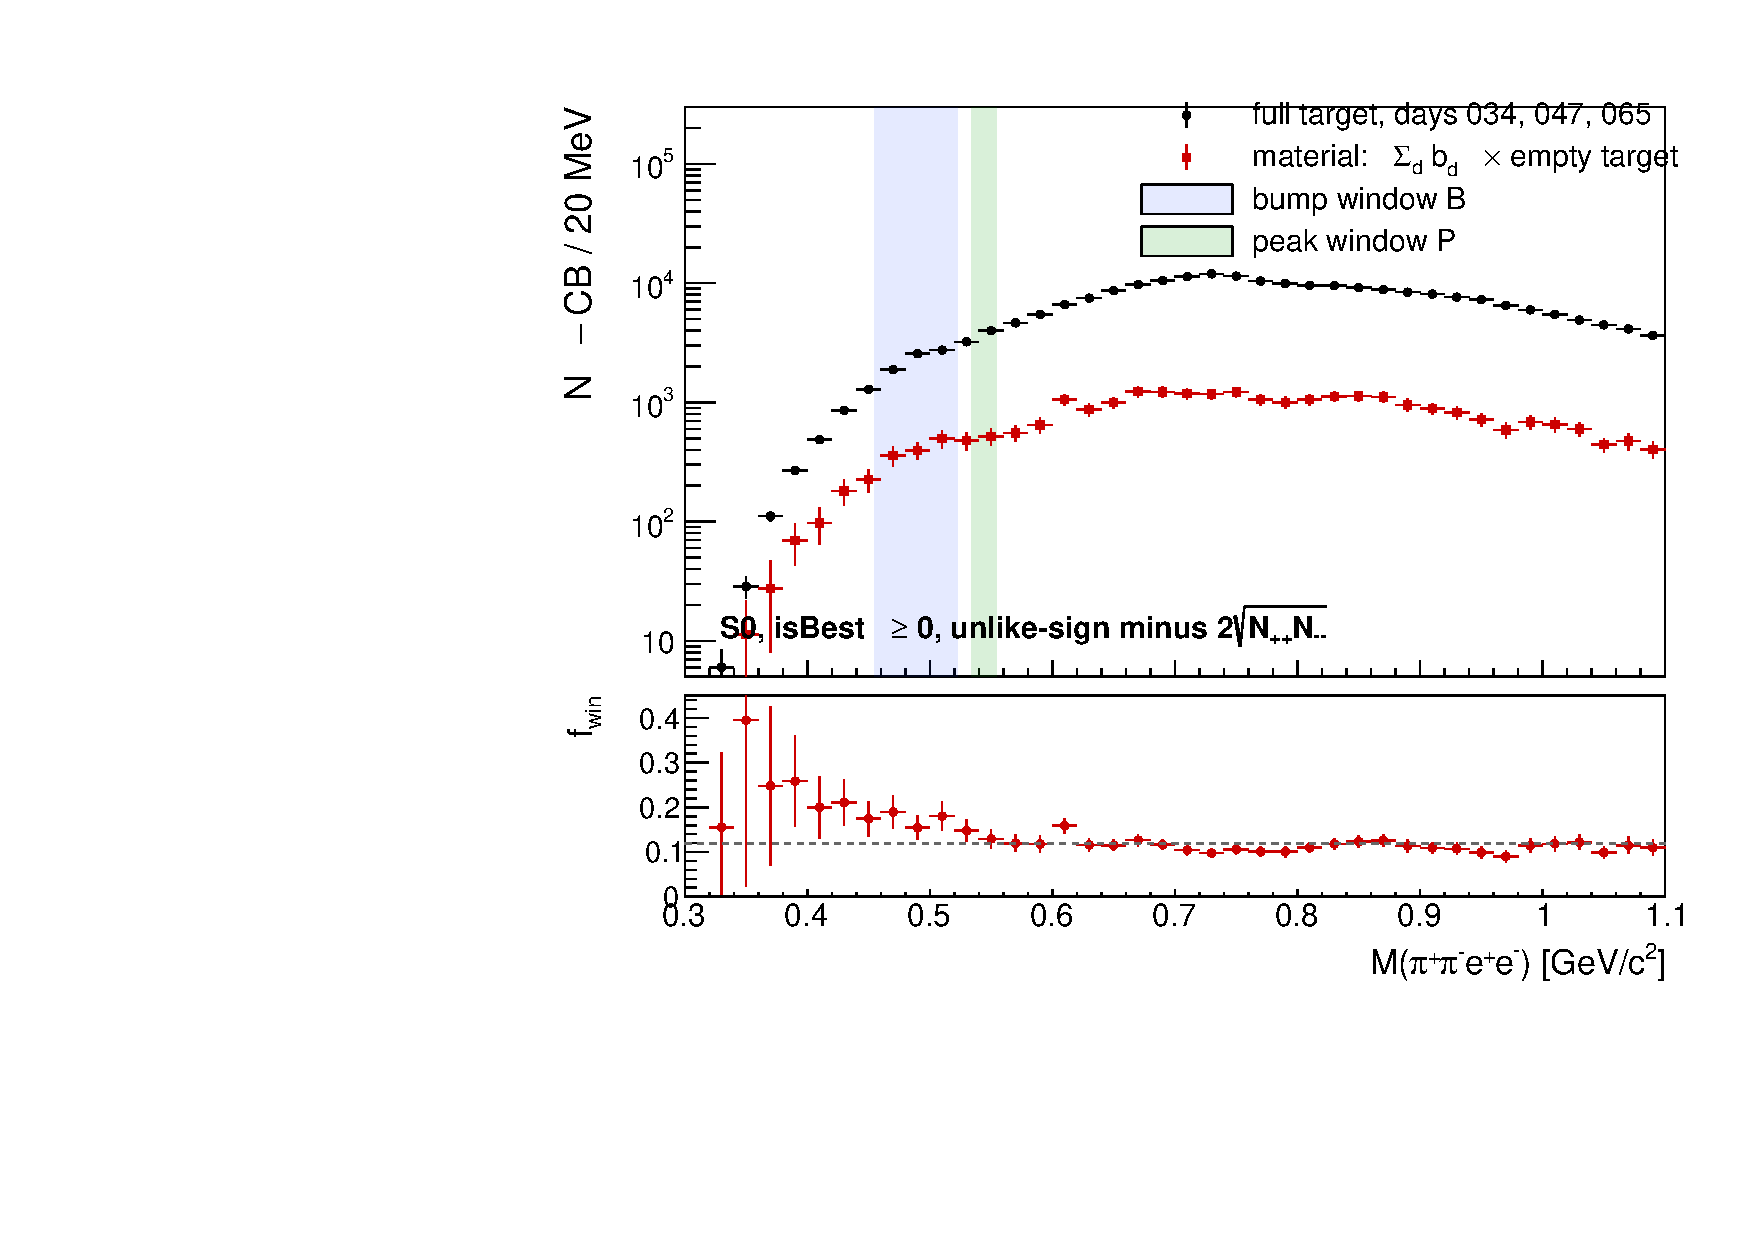
\includegraphics[width=0.6\textwidth]{figs_all/wp2_N1e.pdf}
\caption{\Mfour of $N-\mathrm{CB}$ (S0, isBest $\ge0$), days 034 + 047 + 065.
Selection: data, S0 (PT3 trigger, event vertex in the target region ($\vz>-160$\,mm), \betanew particle identification (pions within $3\sigma$, leptons within $5\sigma$ and with a RICH ring), energy-loss-corrected momenta of all four tracks, all stored combinations of each event (isBest $\ge0$), both pions in the event-vertex fit), all \Mpipi and \Mee; days 034, 047, 065; full target and empty target $\times$ the flux ratio $b_d$ of the day (counts in $-200\le\vz<-170$\,mm); CB $=2\sqrt{N_{++}N_{--}}$ per 20\,\MeVcc bin of \Mfour, $k=1$. Black: full target; red: material $=\sum_{\mathrm{days}}b_d\times$
empty target (20\,\MeVcc bins). Lower pad: \fwin(\Mfour); dashed: the all-\Mfour value 11.9\,\%. Shaded: windows B and P. No fall-back involved.}
\label{fig:N1e}
\end{figure}

\begin{figure}[H]
\centering
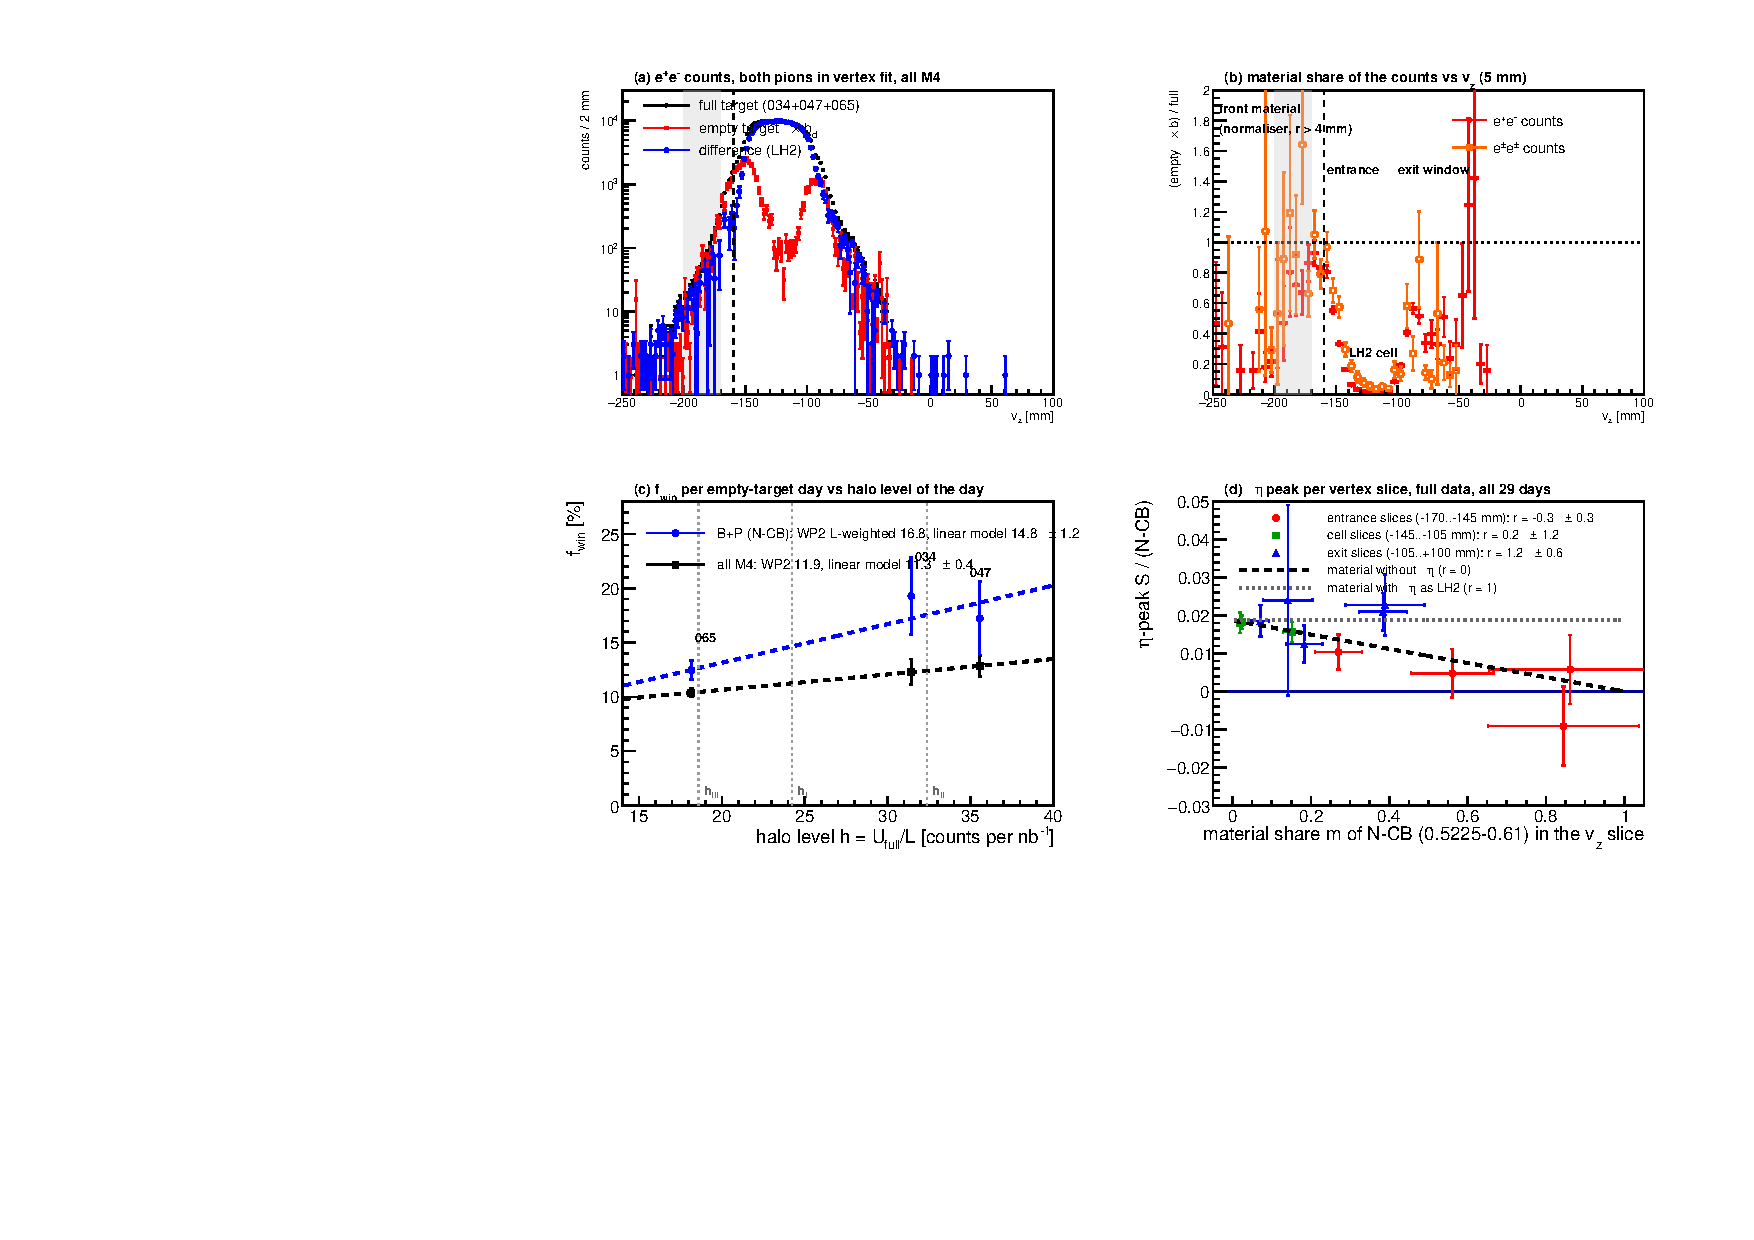
\includegraphics[width=0.86\textwidth]{figs_all/vw2a_fig_cnt.pdf}
\caption{\textbf{What it shows: the $\eta$ signal does not come from the target walls, so the $\eta$ yields are corrected by $1-\feta=0.97$ only, not by the wall share of the counts.}
Selection: data; PT3 trigger, \betanew identification, corrected momenta, isBest $\ge0$, event vertex ($\vz>-500$\,mm) with both pions in its fit, no target-region cut unless stated, all \Mfour. (a), (b) \ee (in (b) also like-sign) combinations, days 034, 047, 065, full and empty target, 2\,mm (a) and 5\,mm (b) bins of $v_z$. (c) S0 ($\vz>-160$\,mm added), $N-\mathrm{CB}$ in the bump and peak windows together (0.4550--0.5225, 0.53364--0.55416\,\GeVcc; also all \Mfour), CB of the window, per empty-target day. (d) all 29 days, full target, 12 slices of $v_z$ from $-170$ to $+100$\,mm: $\eta$-peak content of a fixed Gaussian (0.5439\,\GeVcc, 5.4\,\MeVcc) + pol2 fitted to $N-\mathrm{CB}$ in 0.5225--0.61\,\GeVcc, over $N-\mathrm{CB}$ there; material share of each slice from the three empty-target days.
(a) Vertex $z$ of the \ee combinations (both pions in the vertex fit, all \Mfour), days 034\,+\,047\,+\,065: full target (black), empty target scaled by
the flux ratio of the same day (red), their difference (blue). (b) Material share of the counts per 5\,mm slice of $v_z$: the walls dominate at
the entrance window ($\approx-150$\,mm) and the exit window ($\approx-90$\,mm); inside the LH$_2$ cell they give about 1\,\%. (c) \fwin per
empty-target day against the beam-halo level of that day: \fwin follows the halo, and the empty-target days had a high halo; reweighted to the
luminosity-weighted halo, $\fwin(\mathrm{B+P})=14.7\pm1.1$\,\% instead of 16.8\,\%. (d) The decisive test, on the full data of all 29 days: the
$\eta$-peak content per $N-\mathrm{CB}$ count in each $v_z$ slice against the material share of that slice. If the walls produced no $\eta$, the
points would follow the dashed line (falling to zero at material share 1); if they produced $\eta$ like hydrogen, the dotted line. The
entrance-window slices (red), where the walls give 30--90\,\% of the counts, fall to about zero ($r=-0.27\pm0.34$ for these slices alone; exit-window
slices $r=1.21\pm0.64$); the fit of all slices gives the ratio of $\eta$ per count in the material to that in LH$_2$, $r=0.07\pm0.30$, i.e.\ a material share of the $\eta$ signal $f_\eta=3^{+4}_{-3}$\,\% (adopted, D21, approved by the analyst on 15 November 2026; 1--8\,\%
over the vertex models). An independent check agrees: the share of the $\eta$ peak and of the ECAL-tagged $\eta$ in the cell centre,
$0.566\pm0.045$ and $0.571\pm0.024$, equals the LH$_2$ simulation (0.577), whereas an $\eta$ material share of 16.8\,\% would give 0.497
(excluded at $3.4\sigma$). Figure of the independent verification of WP2 (vw2a).}
\label{fig:feta}
\end{figure}

\subsection{\texorpdfstring{$\eta$}{Eta} efficiency of the event-vertex requirement}
\label{sec:vertexeff}
\notebox{\textbf{Result} (measured after the review of this report by three studies of the PAT files; the decisive one is an independent
verification with its own code, \code{notes_all/ve_verify_note.md}). The mandatory cut $\vz>-500$\,mm keeps
$\varepsilon_{\mathrm{vtx}}(\eta)=\mathbf{0.994\pm0.021}$ of the $\eta$ in the data (above 0.96 at 95\,\% CL) and $0.99970\pm0.00002$ in the
simulation ($0.990\pm0.022$ in the data if $S$ is taken with the CB convention of the report instead of a smooth like-sign CB; D33). The 32\,\%
of the unlike-sign counts without a vertex are mostly not hydrogen events: 87\,\% of their pion pairs cross 8\,mm or more from the beam axis
(35\,\% with a vertex), their pp-elastic content is 0.028 of the cell's, and they contain no tagged $\eta$ and no bump edge; their source is
probably material in front of the cell (a hypothesis). The correction $C_{\mathrm{vtx}}=1.006\pm0.021$ (\sigeta; $1.00\pm0.02$ for the bump
scale) is \emph{not applied}; it is quoted as a one-sided $+2$\,\% ($+4$\,\% at 95\,\% CL). The cut is validated (it removes non-target
background, not target $\eta$), and it is \emph{not} the cause of the low \sigeta: 0.93\,mb would need $\varepsilon=0.46$, excluded by $T$ at
23$\sigma$ and by $E$ at 6.6$\sigma$.}

\textbf{How a combination ends up without a vertex.} PAT copies the event vertex of the DST. In the DST production of the data and of the simulation
alike (Hydra~2.7.4), \code{HParticleVertexFind} with \code{setCut(-170,-30,20)} takes the tracks whose point of closest approach to the beam
axis lies in the finder window ($-170<z<-30$\,mm, $r<20$\,mm) and fits a common point when there are at least two; with one or none it writes
$(-1000,-1000,-1000)$. Below 11 tracks it uses no START or timing information. A combination whose four tracks put two or more into the window
therefore always has a vertex (data 99.7--100\,\%, simulation 99.9--100\,\%); otherwise only other tracks of the event can give it one. In the
data 32.3\,\% of the unlike-sign counts (70.5\,\% / 75.9\,\% of the $e^+e^+$ / $e^-e^-$ counts) have no vertex; in the simulation 0.03\,\% of the
simulated $\eta$ entries. Until now this report could only say that the cut keeps 0.565 of the unlike-sign counts in P and $\ge0.96$ of the simulated entries,
and allowed that the $\eta$ might lose its vertex at the rate of the counts. That is now measured.

\textbf{Procedure} (verifier ve\_verify; the numbers of the two first studies, ve\_data and ve\_sim\_cause, are reproduced exactly):
\begin{enumerate}\setlength{\itemsep}{0pt}
\item \textbf{Entries straight from PAT.} The 29 PAT day files (\code{lep_betanew.list}), the trees of the three hypotheses, every entry with
      isBest $\ge0$ and PT3 (\code{trigbit} $=8192$), corrected momenta and \code{cor_ok} as in FAT, and \emph{no} vertex requirement
      (\code{vtx_fill.C}). The entries with a vertex reproduce the FAT production exactly (4\,783\,467 / 122\,875 / 371\,524 entries; 4\,753\,629 \ee
      entries with \code{cor_ok}).
\item \textbf{Two classes of whole events}: V ($\vz>-500$\,mm) and Nv ($\vz=-1000$\,mm). Each class gets its own CB $=2\sqrt{N_{++}N_{--}}$
      from its own like-sign counts ($k=1$) and the frozen fits of Part~II. The cut $\vz>-160$\,mm and the pion-vertex flag of S0 are \emph{not}
      applied (Nv has no vertex); their efficiencies are known separately: below $-160$\,mm the V counts hold no $\eta$ ($S=-19\pm133$; the
      simulation keeps 0.9973 of C4+C5), and S0/``pre'' is $1.002\pm0.056$ data/simulation (\S\ref{sec:eff}).
\item \textbf{Three $\eta$ measures per class}: $S$, the \Pmain peak content (frozen Gaussian 0.5439\,\GeVcc / 5.4\,\MeVcc + pol2 in
      0.5225--0.61 on $N-\mathrm{CB}$); $T$, the ECAL-tagged $\eta\to\pipi\piz$ (photon with $0.119\le M(\ee\gamma)<0.173$\,\GeVcc,
      \Mee$<0.10$, fit of m5c with 0.5463 / 6.2\,\MeVcc + pol2); $E$, the bump edge step (four \Mpipi slices, edge fixed). $T$ and $E$ do not
      depend on the CB of the peak; $E$ does not use the ECAL. Because the CB of Nv has a statistical hole at $m_\eta$ (below), $S$ is also
      taken with a \emph{smooth like-sign CB}: $N_{++}$ and $N_{--}$ of the class are each fitted with a polynomial (pol3, pol4 or pol5, from
      0.45 or 0.48 to 0.66 or 0.70\,\GeVcc: 12 variants; $\chi^2=94.9/95$ and 100.5/95 for pol4 in 0.45--0.70), the CB is $2\sqrt{f_{++}f_{--}}$
      per 2.5\,\MeVcc bin, and \Pmain is fitted as before; the quoted $S$ is the mean of the 12 variants (rms 30 counts). This is not the CB
      convention of the report (D33).
\item \textbf{Efficiency}: $\varepsilon_{\mathrm{vtx}}=X_V/(X_V+X_{Nv})$ for each measure $X$; the classes are disjoint events, so the errors
      of $X_V$ and $X_{Nv}$ are independent ($S$ with the nominal CB: fit error $\times$ event-group factor, 1.02--1.03; $E$: fit error $\times1.2$,
      Part~II's first calibration, kept as a conservative choice although the bootstrap of \S\ref{sec:bedge} finds the fit error right, plus
      the model rms). The three values $S$ (smooth CB), $T$ and $E$ are combined with inverse-variance weights as
      if independent; they use the same Nv events ($S$ and $T$ share about 30\,\% of the counts), but $T$ carries 81\,\% of the weight (D33).
\item \textbf{Simulation}: the same selection on the simulated PAT files ($\eta$ and std sets), with the truth classes C2--C5 tagged from the
      GEANT ids and creation processes (\code{vtx_sim.C}).
\end{enumerate}

\begin{table}[H]
\centering
\caption{$\eta$ efficiency of the event-vertex cut $\vz>-500$\,mm. Data: 29 PAT day files, PT3, isBest $\ge0$, \code{cor_ok}, no other cut;
classes V (vertex) and Nv (no vertex); CB $=2\sqrt{N_{++}N_{--}}$ of each class, $k=1$; counts, not normalised to luminosity. Errors: $S$ with
the nominal CB: fit error with the event-group factor (stat$_g$) and model $=$ rms over the verifier's grid (order 1--4, upper bound 0.58--0.65,
lower bound 0.5225--0.5275, width $\pm0.5$\,\MeVcc; 152 pairs with $p>0.05$); the other $S$ rows: plain fit errors (the group factor,
1.02--1.03, changes $\varepsilon$ by less than 0.002); $E$: fit error $\times1.2$ (conservative; Part~II's first calibration) and model $=$ rms over 18 variations
applied to both classes. V contains the combinations of ``pre'' and adds those with $-500<\vz\le-160$\,mm, whose $S$ is $-19\pm133$; hence $S(\mathrm{V})=4657$
against $S(\mathrm{pre})=4671$ (both with the verifier's code), and $T(\mathrm{V})=3297$ (verifier's code) against 3314 (Part~II): the differences
are within the errors. Simulation: same selection, truth classes, unweighted. Sources: \code{tables_all/vtx_ana.txt}, \code{vtx_ana2.txt},
\code{vtx_ana3.txt}, \code{vtx_sim.txt}, \code{vtx_numbers.txt} (verifier ve\_verify), \code{fix2_numbers.txt} ($E$ errors, combinations). No
fall-back involved.}
\label{tab:vtx}
\footnotesize
\begin{tabularx}{\textwidth}{@{}>{\raggedright\arraybackslash}p{5.3cm} r r L@{}}
\toprule
measure & $X_V$ & $X_{Nv}$ & $\varepsilon_{\mathrm{vtx}}=X_V/(X_V+X_{Nv})$ \\
\midrule
$S$, nominal CB (shown, not used; see text) & $4657\pm397$ & $902\pm411$ & $0.838\pm0.063\pm0.060$ \\
$S$, unlike-sign counts only (no CB) & $4646\pm370$ & $165\pm324$ & $0.966\pm0.065$ \\
$S$, smooth like-sign CB (12 variants) & $4670\pm370$ & $263\pm324$ & $0.947\pm0.063$ \\
$T$, ECAL-tagged $\eta$ & $3297\pm110$ & $-4\pm77$ & $1.001\pm0.023$ \\
$E$, bump edge step & $1241\pm91$ & $21\pm96$ & $0.983\pm0.075\pm0.028$ \\
\midrule
\textbf{$S$ (smooth CB) $+$ $T$ $+$ $E$} & & & $\mathbf{0.994\pm0.021}$, $\chi^2=0.7/2$; $>0.96$ (95\,\% CL) \\
$S$ (nominal CB) $+$ $T$ $+$ $E$ & & & $0.990\pm0.022$, $\chi^2=3.3/2$ (CB convention of the report) \\
$S$ (smooth CB) $+$ $E$, no ECAL & & & $0.961\pm0.049$ \\
\midrule
\multicolumn{4}{@{}l}{\emph{Simulation} (simulated entries; lost entries)} \\
C4 $+$ C5 (peak), all \Mfour & 573\,129 & 171 & $0.99970\pm0.00002$ (peak window 0.99975) \\
\quad C5 / C4 & 572\,822 / 307 & 171 / 0 & 0.99970 / 1 ($>0.990$ at 95\,\% CL) \\
C2 $+$ C3 (bump), all \Mfour & 2852 & 4 & $0.9986\pm0.0007$ (bump window $0.9981\pm0.0009$) \\
\midrule
\multicolumn{4}{@{}l}{\emph{Survival of the counts} (not an efficiency): all \ee counts 0.6773; \ee counts in P 0.565; $e^+e^+$ 0.295, $e^-e^-$ 0.241} \\
\bottomrule
\end{tabularx}
\end{table}

\begin{figure}[tp]
\centering
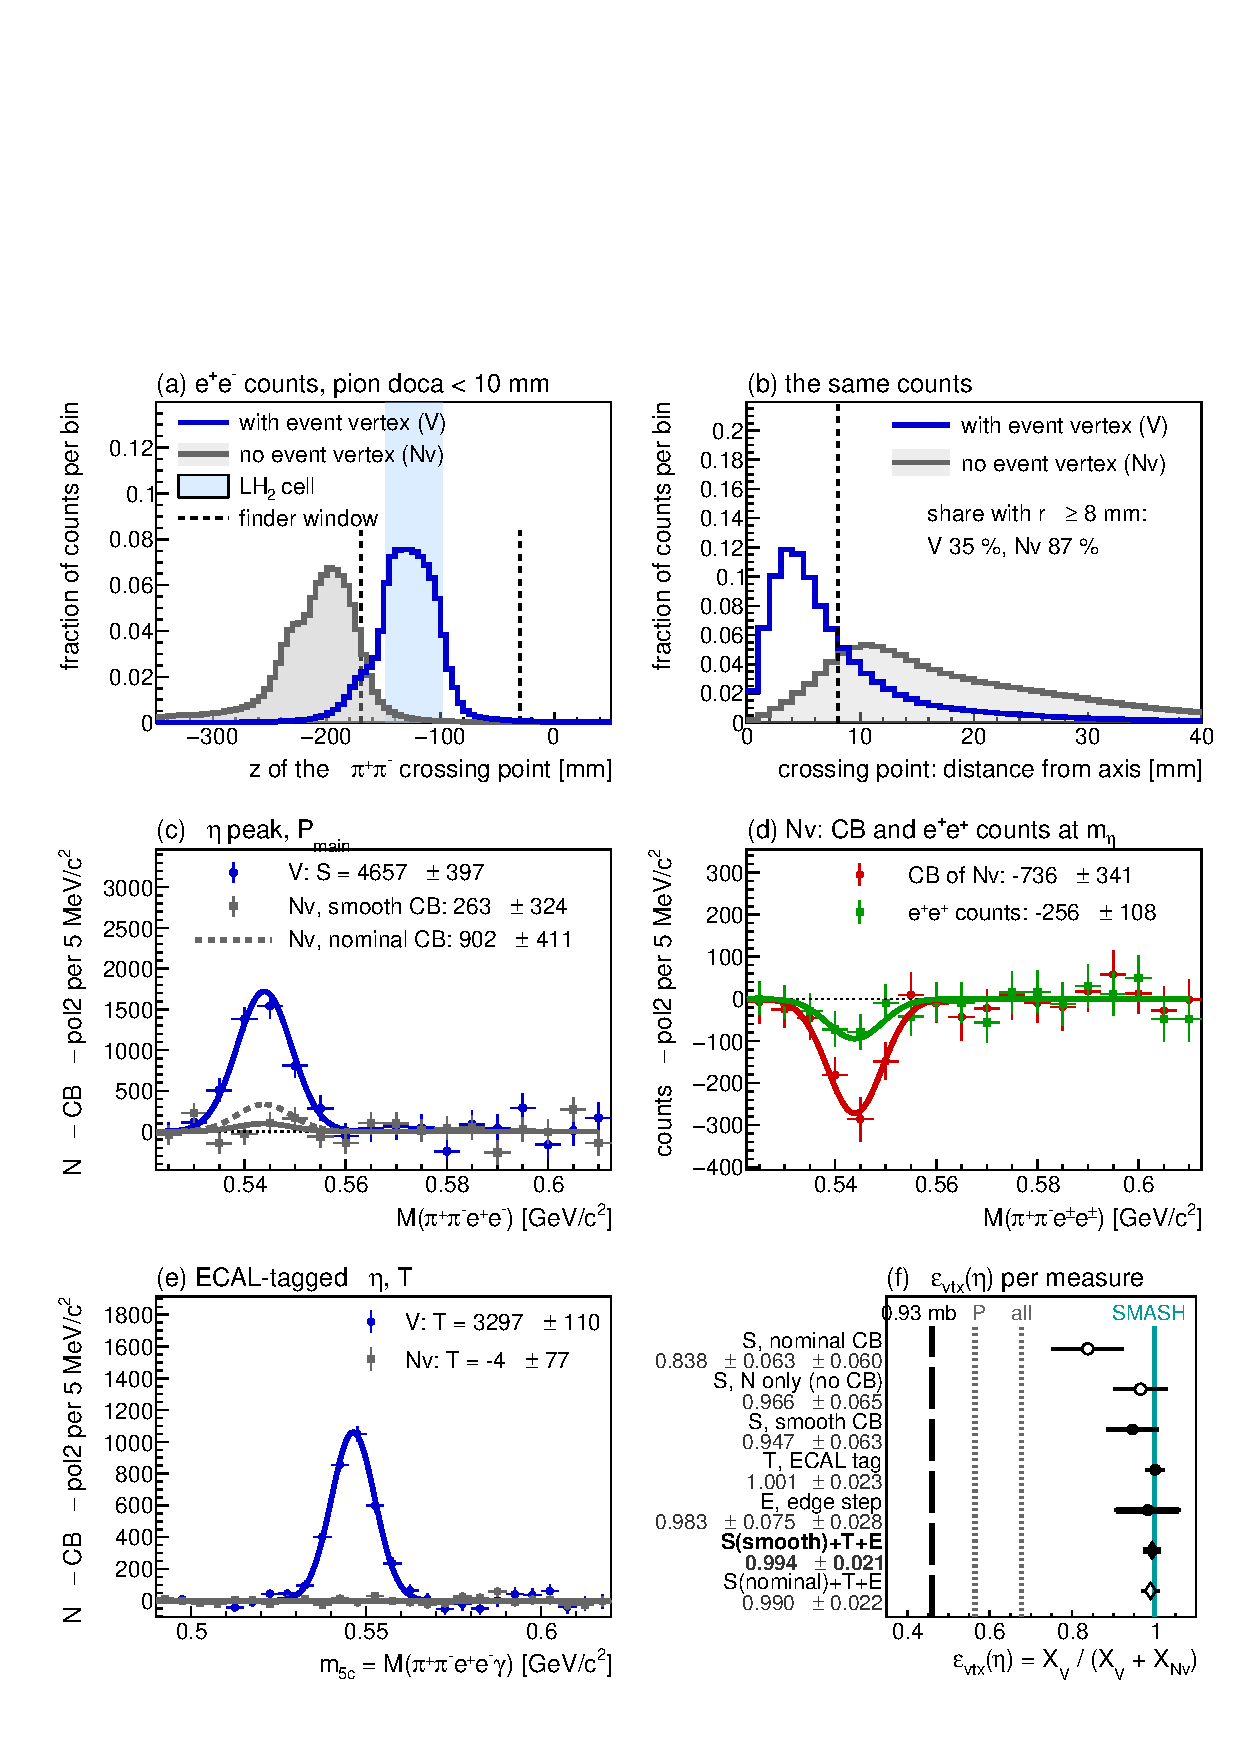
\includegraphics[width=0.97\textwidth]{figs_all/fix2_vtx_fig_cnt.pdf}
\caption{$\eta$ efficiency of the event-vertex cut.
Selection: data from the 29 PAT day files: PT3 trigger, \betanew identification, corrected momenta, isBest $\ge0$; no target-region and no pion-vertex cut; whole events with (V, $\vz>-500$\,mm) and without (Nv) a vertex, each with the CB of its own like-sign counts; (a, b) pion tracks within 10\,mm of each other; (c, d) \Pmain fit in 0.5225--0.61\,\GeVcc. Data, 29 PAT day files, PT3, isBest $\ge0$, \code{cor_ok}; V (event vertex) blue, Nv (none)
grey; counts, not normalised to luminosity. (a, b) $z$ and distance from the beam axis of the crossing point of the two pion tracks (\ee combinations, pion
distance of closest approach $<10$\,mm; unit area); the Nv $z$ is partly shaped by the selection (at most one track in the finder window).
(c) $\eta$ peak, $N-\mathrm{CB}-$pol2 of the \Pmain fit (5\,\MeVcc bins): V; Nv with a smooth like-sign CB (squares: pol4, 0.48--0.70, $S=265$;
legend: mean of the 12 variants) and, dashed, with the nominal CB; legend errors of the nominal-CB fits with the event-group factor. (d) Nv: the
frozen Gaussian fitted to the CB (red) and to the $e^+e^+$ counts (green). (e) ECAL-tagged $\eta$ in m5c. (f) $\varepsilon_{\mathrm{vtx}}$ as in
Table~\ref{tab:vtx} (open: not used for the result; $E$: thick bar stat $\times1.2$, thin bar with the model rms); lines: simulation 0.9997,
survival of the counts 0.565 (P) and 0.677 (all), and 0.46, needed for \sigeta $=0.93$\,mb. Macro \code{plots/all_report/fix2_vtx_fig.C}. No fall-back
involved.}
\label{fig:vtx}
\end{figure}

\textbf{Why $S$ with the nominal CB is low.} $S(\mathrm{Nv})=902\pm411$ (2.2$\sigma$) is not an $\eta$ signal: (i) the same
fit on the unlike-sign counts alone (no CB) gives $165\pm324$; (ii) the CB of Nv itself has a Gaussian dip at $m_\eta$ of $-736\pm341$ counts
(Fig.~\ref{fig:vtx}d), made by the $e^+e^+$ counts ($-256\pm108$, a 2.4$\sigma$ downward fluctuation; $e^-e^-$: $+73\pm283$); because the
like-sign combinations lose their vertex 2.2--2.4 times more often than the \ee combinations (70.5\,\% and 75.9\,\% against 32.3\,\%), the CB is 58\,\% of $N$
in Nv (13\,\% in V), and a hole in $N_{++}$
moves $S(\mathrm{Nv})$ by several hundred counts; (iii) with a smooth like-sign CB $S(\mathrm{Nv})=263\pm324$ (12 variants, rms 30);
(iv) a free fit of the Nv ``peak'' is $3.75\pm1.0$\,\MeVcc wide, 1.65$\sigma$ below the detector resolution (5.4\,\MeVcc); a real 2$\sigma$ peak can
fluctuate that much, so this is only weak support; (v) frozen-width fits at 39 other positions in Nv have pulls of rms 0.93, so the errors are right and the 2.25 pull at $m_\eta$ comes from
the CB; (vi) $T$ and $E$, which would follow any real $\eta$ (target or material), are zero in Nv. The nominal-CB value is therefore a CB
fluctuation; it is listed but not used (its model grid gives 0.60--0.87 only because $S(\mathrm{Nv})$ moves). By pion crossing radius the
nominal $S$ gives $1.001\pm0.037$ at $r<5$\,mm and $1.04\pm0.10$ at 5--8\,mm, and the apparent loss sits only at $r\ge8$\,mm, where the CB of
Nv is.

\textbf{Does the photon tag work without a vertex?} Yes: the \piz peak in $M(\ee\gamma)$ is present in Nv ($61\,648\pm4364$ at 0.1361\,\GeVcc,
$\sigma=18.4$\,\MeVcc, against $539\,887\pm2342$ at 0.1416, $\sigma=13.5$\,\MeVcc in V). It is 5.5\,\MeVcc lower and 36\,\% wider, because
without an event vertex the ECAL uses the cluster vertex for the photon direction, but most of it lies inside the tag window. For a target event
that lost its vertex the cluster vertex is at the right place, so $T$ measures the loss of target $\eta$ (well founded, not proven with target
events); $E$, which does not use the ECAL, agrees.

\textbf{Origin of the combinations without a vertex} (ve\_data, ve\_sim\_cause, checked by the verifier). The evidence that does not depend on how the
combinations were selected comes first:
\begin{itemize}\setlength{\itemsep}{0pt}
\item \emph{Off the beam axis.} 87\,\% of the Nv pion pairs cross 8\,mm or more from the axis, against 35\,\% for V (Fig.~\ref{fig:vtx}b). The
      finder does not cut on $r$ below 20\,mm, so this is not made by the selection.
\item \emph{Not hydrogen.} The pp-elastic content per two-track event of the hadron production is $0.028\pm0.003$ of that in the cell for
      upstream events without a vertex: about 97\,\% of them are not p+p on hydrogen. Caveats: the elastic acceptance of upstream events was not
      modelled, and only three days (036, 049, 062) of the June hadron production were used.
\item \emph{Different events.} CB$/N$ in P is 0.58 (Nv) against 0.13 (V); the Nv share of the \ee counts follows the beam periods (days 034--045:
      0.31, 046--053: 0.37, 059--067: 0.275), is flat over the sectors (0.317--0.327), and is higher without a START hit (0.53 against 0.30), as
      particles that miss the START would be.
\item \emph{Target events keep their vertex.} When the two pions cross inside the cell ($-170\le z<-85$\,mm, $r<8$\,mm), only 0.15\,\% of the combinations
      lack a vertex (3339 of 2.19 million; ve\_data).
\item \emph{Place} (partly shaped by the selection). The Nv pion pairs cross at $z\approx-200$\,mm (mode $-197.5$, mean $-207$\,mm), about
      5--6\,cm in front of the upstream end of the LH$_2$ cell (7--8\,cm from its centre); the V pairs at $-165$ to $-95$\,mm (Fig.~\ref{fig:vtx}a).
      Since a combination without a vertex has at most one track in the finder window, its pion crossing and the median $z$ of its tracks are pushed
      outside the window by construction, so the position alone is not independent evidence. Not forced by the selection is that the median track
      $z$ of Nv stays at $-214$ to $-197$\,mm at all polar angles; a timing or reconstruction distortion would change with the angle.
\item \emph{Material there} (hypothesis). In the HGeant target geometry the LH$_2$ cell spans $-148.4$ to $-98.6$\,mm; from $-229$ to $-174$\,mm
      sit the steel holder, copper and an LH$_2$ ring ($r>8$\,mm), the steel beam tube (inner radius 7.5\,mm) runs from $-243$\,mm, steel flanges
      at $-252$ to $-229$\,mm. Beam halo hitting this material is a natural source, but it is not proven (to be confirmed with the target
      drawing), and it leaves one fact unexplained: p+A collisions at 4.5\,GeV make $\eta$ mesons, yet the Nv counts show none (next item).
\item \emph{No $\eta$ physics.} $T(\mathrm{Nv})=-4\pm77$ ($27\pm67$ with the code of ve\_data), $E(\mathrm{Nv})=21\pm96$, and the structure
      near 0.74\,\GeVcc ($\omega$ region) is absent too (Nv/V $=-0.12\pm0.06$). Per period, with the code of ve\_data (its overall value
      $\varepsilon_T=0.992\pm0.020$), $\varepsilon_T=1.013\pm0.033$, $0.993\pm0.097$, $0.924\pm0.045$, $1.006\pm0.030$ (I, IIA, IIB, III): consistent
      with 1 in every period within 1.7$\sigma$ (IIB is the lowest). The nominal-CB $S$ of period III gives $0.700\pm0.088$ ($S(\mathrm{Nv})=515\pm196$);
      about half of it is a dip of the CB (unlike-sign counts alone $254\pm154$, Gaussian content of the CB $-273\pm161$; verifier), and $T$ and $E$
      show nothing there. The period steps of the survival of the counts (0.62--0.72 per day) belong to the non-target combinations.
\item \emph{Simulation.} It generates vertices only in the cell and has no beam halo, so it has no such combinations; this is nearly all of the
      data/simulation difference of the survival of the counts. Target events of the data lose their vertex at most at the 1\,\% level: 2.19\,\% of the data
      combinations of target events (vertex inside the cell; days 036, 049, 062) have at most one own track in the finder window (simulation 0.09\,\%;
      the data track $z$ resolution is worse, rms 23.7 against 17.9\,mm, and the beam axis is off by (2.7, $-2.3$)\,mm), and in the simulation such
      a combination loses its vertex with probability 0.33--0.38 (other tracks of the event rescue the rest); $0.0219\times0.35\approx0.8$\,\% is an upper
      estimate (ve\_sim\_cause: $\varepsilon=0.992\pm0.010$), consistent with the measurement.
\end{itemize}

\textbf{Consequences.}
\begin{itemize}\setlength{\itemsep}{0pt}
\item $C_{\mathrm{vtx}}=\varepsilon_{\mathrm{sim}}/\varepsilon_{\mathrm{data}}=0.9997/0.994=1.006\pm0.021$ for \sigeta (below 1.04 at 95\,\% CL;
      physically not below 0.9997, since $\varepsilon_{\mathrm{data}}\le1$). For the bump, $T$ (the same decay) and $E$ give $1.000\pm0.022$
      (0.999 without the factor 1.2 on $E$) against 0.9986 simulated: $1.00\pm0.02$. The ratios (DR, \BRG, \BRA, the X17 BR limit) are free of it.
\item \textbf{Not applied}: compatible with 1. It enters the error budget as a one-sided $+2$\,\% ($+4$\,\% at 95\,\% CL) on the absolute $\eta$
      scales (Table~\ref{tab:S1}, last row; known-sign list of \S\ref{sec:p2}; Table~\ref{tab:v8sigma}). Applied, 0.429\,mb would become 0.4315\,mb.
\item \textbf{Not the cause of the low value.} \sigeta $=0.93$ / 1.14\,mb would need $\varepsilon_{\mathrm{data}}=0.46$ / 0.38; excluded by $T$
      (23 / 26.5$\sigma$), $E$ (6.6 / 7.6$\sigma$, with its statistical error $\times1.2$), the smooth-CB $S$ (7.8 / 9.1$\sigma$) and even the
      nominal $S$ (4.3 / 5.3$\sigma$). Dividing by
      the survival of the counts (0.565--0.68) would be wrong: it would count upstream non-hydrogen counts (and their CB) as lost $\eta$.
\item \textbf{The cut is validated}: it removes non-target background (CB$/N=0.58$), not target $\eta$.
\item \textbf{Superseded}: ``the simulation keeps $\ge0.96$'' (0.968 std, 0.976 lep, 0.959 $\eta$ set) was the ratio of FAT to PAT entries of whole
      simulated sets (Part~I), not the vertex efficiency of the $\eta$ (0.9997); the arithmetic of the first data study (``0.42\,mb'' with the data
      efficiency, ``0.49\,mb'' with the nominal $S$) used 0.96 instead of 0.9997 and reads 0.436 and 0.51\,mb (verifier).
\item \textbf{Not checked}: which vertex condition the elastic luminosity analysis used. If it used none, the upstream elastic events would add
      about 1\,\% to $L$ (593 against 53\,966 elastic events, ve\_sim\_cause). If it required the DST vertex, its two-track elastic events cannot be
      rescued by other tracks, and the per-track probability to miss the finder window (data 0.08--0.16, simulation 0.05--0.08, measured on \ppee
      tracks) could make the data/simulation difference of the elastic vertex efficiency several per cent. This case is not estimated here; it has
      to be checked in the luminosity analysis.
\item \textbf{K$^0_S$} (side check): the cut keeps 0.72--0.85 of the K$^0_S$ in the data (simulation 0.991--0.996), so it explains at most a
      factor 1.4 of the K$^0_S$ deficit (0.29 of SMASH, \S\ref{sec:before}). The loss is attributed to the displaced decay of the K$^0_S$: its part
      without a vertex does not sit in the upstream box of the pion crossing (2.2 K$^0_S$ per $10^4$ Nv counts there against 18.1 elsewhere, ve\_data).
\end{itemize}

\subsection{Efficiencies and the QED check of the bump simulation}
\label{sec:eff}
\tabin{wp8_tableP1.tex}

Table~\ref{tab:P1} gives the acceptance $\times$ efficiency of the signal classes (WP8, \code{wp8_sim.C}); with the 1.069\,mb of the
simulation study it reproduces Part~I's efficiencies of all five classes to 0.1\,\%. \flag{The verifier v8 found that the SMASH
$\sigma(\eta)$ of the simulated sample is 1.0694\,mb ($N_\eta=2.364\times10^8$ in $10^{10}$ events); 1.0665\,mb is a 200-file sub-sample, so the
efficiencies of Table~\ref{tab:P1} are 0.28\,\% too high.} Simulated S0/``pre'': 0.914 (C2), 0.936, 0.948, 0.933, 0.930 (C6). Accepted C2 in
B with \Mee$\ge20$\,\MeVcc: 0.376 (reconstructed), 0.377 (true); generator fraction 0.269. \textbf{Pion-vertex efficiency} S0/``pre'' (on the base
``pre'' of this report): $\eta$ peak data $0.941\pm0.052$ against simulation 0.940 (data/sim $1.002\pm0.056$; Part~II gives $0.940\pm0.041$ in the
data on its base ``peak nominal''); ECAL-tagged $\eta$ $0.933\pm0.013$ vs 0.933 (emulated tag)
or 0.947 (truth), $1.000\pm0.014$. The $\pm2.5$\,\% of family S12 is therefore conservative and kept.

\textbf{eps2 QED check} (Table~\ref{tab:eps2}). The specification asked whether the simulated bump C2 has the QED fraction of pairs with
\Mee$\ge20$\,\MeVcc. (a) \textbf{Generator}: HGeant samples the \piz Dalitz pair mass from a 0.1\,\MeVcc histogram of Kroll--Wada $\times$
a $\rho$-pole form factor; its fraction above 20\,\MeVcc (0.2688) equals Kroll--Wada $\times$ the PDG form factor (0.2693): PASS. (b)
\textbf{Decay angle}: the HGeant source (\code{gdalet.F}) decays $\gamma^*\to\ee$ \emph{isotropically}, while QED gives $1+\cos^2\theta^*$;
PLUTO (lepton set, 124\,378 decays read on vae25) has the QED angle ($\langle\cos^2\theta^*\rangle=0.4025\pm0.0012$ and $0.3970\pm0.0017$,
QED 0.400): \textbf{FAIL for C2}. (c) Effect: a toy with the HADES acceptance (18--85$^\circ$, momentum cuts) gives
$\varepsilon(\mathrm{QED})/\varepsilon(\mathrm{iso})=0.880$ (all), and the full-simulation lepton/standard closure, corrected for the pair-mass
spectrum, 0.891; the verifier v8 confirmed it with its own toy (0.875 at $p_e>0.06$\,\GeVc). These toys and the closure give
a simulated C2 efficiency 12--14\,\% too high ($\varepsilon_{\mathrm{QED}}/\varepsilon_{\mathrm{iso}}=0.875$--0.891), which explains the ``unexplained'' closure 0.891 of prompt \piz pairs in Part~I; for the bump counts of this analysis the per-count QED weights of the full simulation give about 16\,\% (0.86 at the edges, \S\ref{sec:c2recon}). (d) The tagged $\eta$ shares above 20\,\MeVcc agree
(data/sim $1.06\pm0.15$ fit, $0.95\pm0.13$ truth: PASS within the simulation statistics), but this test is blind to the angle effect, which
scales C2 almost uniformly in \Mee.

Refitting the whole chain with the C2 templates scaled by the toy / closure factors gives: \aEta $+9/+12$\,\%, \aB $+9/+12$\,\%, \BRG
$-7/-9$\,\%, \BRA $-9/-12$\,\%, DR $-8/-10$\,\%, \Ybump $+3.4/+1.5$\,\%, $\kappa$ $-3.4/-2.6$\,\%, $Y_4$ $+8.4/+6.5$\,\%, $Y_5$ $-1.3/-1.0$\,\%;
$\sigma_\eta$ from the peak is unchanged ($-0.1$\,\%). With the angle correction DR$_F$ moves from 1.17 to 1.09--1.10 and $f_\eta$(edge) from 0.39
to about 0.42, close to \aP $=0.418$ (supporting indications, not proof). \textbf{Not applied} (frozen procedure): entered as family S12 with
known sign (Table~\ref{tab:S12}) and as a labelled variant. The bump-edge measurements of \S\ref{sec:bedge} and \S\ref{sec:edgeu} apply it, since D38 (approved) with
per-count QED weights: a per-count average of the QED weight along the circle of the lost photon, 0.860--0.861 at the edges and 0.876 for the
ECAL-tagged combinations (\S\ref{sec:c2recon}). They give 0.423 per slice (0.418 with the constant factor of D35) and 0.426 in $u$, against
0.392 and 0.390 without the correction.

\tabin{wp8_eps2.tex}

\subsection{Spec.\ Table~P2: physics quantities}
\label{sec:p2}
\textbf{\sigeta} is computed from the peak side bands, the estimator that passed the closure test (WP7/WP8 decision; the F-main value is a
cross-check):
\begin{equation}
\sigma(pp\to\eta X)=a_P\times\sigma_{\mathrm{SMASH}}(\eta)\times C_{\mathrm{sec}}(1-f_\eta),\qquad
a_P=\frac{Y_{\mathrm{peak}}}{(\mathrm{C4}+\mathrm{C5})_{\mathrm{SMASH}}\ \text{in P}},
\label{eq:sigma}
\end{equation}
with $\aP=5087.97/12\,164.94=0.418249$.
WP8 gives $0.437\pm0.037\pm0.070\pm0.026^{+0.035}_{-0.037}$\,mb. The verifier v8 reproduced it to $10^{-5}$ and corrected four items:
(i) the branching ratios of the simulation are PDG 2020; PDG 2026 has $\eta\to\pipi\piz$ $23.02\pm0.25$\,\%, $\pipi\gamma$ $4.28\pm0.07$\,\%,
$\ppee$ $(2.76\pm0.16)\times10^{-4}$ ($\piz\to\ee\gamma$ unchanged), which rescales C2, C3 by 1.00436, C4 by 1.01422, C5 by 1.02985 and \sigeta by
$-2.19$\,\%; (ii) $\sigma_{\mathrm{SMASH}}=1.0694$\,mb (+0.28\,\%); (iii) \Csec of the peak, 1.0116 (+0.06\,\%); (iv) the composition of the
peak in the systematic error (v8: $\pm9.6$\,\% from the prior $\kappa=1\pm0.2$).

\textbf{Composition of the peak from the data} (review, reviewer finding; \code{fix_numbers.py}). The prior $\kappa=1\pm0.2$ is a fall-back
number. The data measure the mix of the peak in three ways, all with the PDG 2026 rescaling:
\begin{itemize}\setlength{\itemsep}{0pt}
\item \emph{Peak side bands per \Mee class}: E1 $2380\pm334$, E2 $2780\pm372$ counts (stat $\oplus$ MC; E2 also $\pm395$ from its own displaced-window
      closure, \S\ref{sec:closure}) against the SMASH shapes (C4: 4946 / 942, C5: 2201 / 4349 counts in E1 / E2). With $\rho=1$ (PDG BR) this
      gives the direct-decay scale $a=0.592\pm0.139$ and the conversion scale $a\kappa=0.218\pm0.097$, $\kappa=0.37\pm0.23$; the data peak is
      more E2-like than SMASH (E2 share 0.546 against 0.425 with the C4/C5 shapes of this fit, 0.423 in WP8's sums; per class $\aP(E1)=0.33$, $\aP(E2)=0.53$).
\item \emph{X17 2D fit} (all 1050 cells, $r=0$, \S\ref{sec:x17d}): $N_5=3659\pm503$ and $N_4=1648\pm383$ against the SMASH references 7681 and 6751
      counts: $N_5/N_5^{\mathrm{ref}}=0.476\pm0.065$, $N_4/N_4^{\mathrm{ref}}=0.244\pm0.057$ (PDG 2020: 0.491, 0.248), $\kappa=0.51$.
\item \emph{F-main}: E1+E2 $\kappa=0.50\pm0.16$; E2 $\aEta\rhod=0.488$ (C2-dominated \aEta times the direct-decay factor).
\end{itemize}
Weighted, the direct-decay route gives $a=0.497\pm0.059$ and the conversion route $a=0.237\pm0.049$ (stat). \aP $=0.409$ (PDG 2026) lies between
them because it mixes both. The \textbf{composition systematic} is half their difference relative to \aP, $\pm31.8$\,\% (X17 fit alone
$\pm28$\,\%, side bands alone $\pm46$\,\%). Which route is right is not known: SMASH may overestimate the conversions (material or the
close-pair efficiency in the simulation) or underestimate the direct decays. As alternative values: \sigeta from the direct-decay route
$0.52\pm0.06\,(\mathrm{stat})$\,mb (X17 fit 0.50, side bands 0.62), from the conversion route $0.25\pm0.05$\,mb. The analyst ruled on
15 November 2026 (D31, option (a)) that the composition is taken from the data, provisionally, until the separate test of D32: if the data are
shown to lose close pairs, the direct-decay route becomes the natural headline with a much smaller composition term (and the bump gives 0.57\,mb
with the conversions $\times0.48$); if not, the adopted value with its $\pm32$\,\% stays.

\textbf{The adopted value} (v8 corrections (i)--(iii), the composition from the data):
\begin{align}
\sigma(pp\to\eta X)&=0.429\pm0.036\,(\mathrm{stat})\pm0.157\,(\mathrm{syst})\pm0.025\,(\mathrm{MC})\,^{+0.041}_{-0.043}\,(\mathrm{norm.})\ \mathrm{mb},\nonumber\\
\sigma(pp\to\eta X)/\sigma_{\mathrm{SMASH}}&=0.401\pm0.157,
\end{align}
a total uncertainty of 39.2\,\% (the syst includes the peak-tail family of D40, approved, $\pm8.8$\,\%; 38.3\,\% without it; v8 with the prior: $\pm0.079$ syst, 22.9\,\% total), and separately the production model
$^{+0.08}_{-0.03}$\,mb (D29, ruled; end of this subsection). The normalisation error is $L$ 6.9\,\% $\oplus$
$\Csec(1-\feta)$ $^{+3.1}_{-4.1}$\,\% $\oplus$ PDG BRs of the peak mix (3.15\,\%) $\oplus$ the period normalisation of Part~II ($\pm5$\,\%: the
per-day rates change in steps between the beam periods for a reason not yet proven (Part~II: they follow the beam-halo level, an
indication), and the per-period tests of Table~\ref{tab:periods}, with
12--33\,\% errors, cannot exclude such a shift of the integrated yield) $=^{+9.6}_{-10.0}$\,\% ($^{+8.2}_{-8.6}$\,\% without the period term;
\code{fix2_numbers.txt}). It is labelled \textbf{PRELIMINARY} (fall-back of the specification applied by analogy, D28; ruled by the analyst on 15 November 2026: the
label stays, because the make-up of the peak is open, while its first reason, the event-vertex efficiency, is now measured). It is \emph{not}
called a lower value: the one-sided items (live time, sorter, \code{cor_ok}; together $+11$--13\,\%) and the measured event-vertex factor
($C_{\mathrm{vtx}}=1.006\pm0.021$, \S\ref{sec:vertexeff}; at most $+4$\,\% at 95\,\% CL) would raise it, but known-sign items of about the same
size would lower it (the measured peak width $-10.8$\,\%, $\feta=12$\,\% $-9$\,\%, the $y$-only reweighting $-8$\,\%; list below).

\textbf{Known-sign items in both directions} (not applied; central value of \sigeta after each, \code{fix_numbers.txt}; the vertex rows were
replaced after the measurement of \S\ref{sec:vertexeff}, \code{vtx_numbers.txt}):
\begin{center}\small
\begin{tabular}{@{}>{\raggedright\arraybackslash}p{9.6cm} >{\raggedright\arraybackslash}p{3.4cm} r@{}}
\toprule
item & factor & \sigeta [mb] \\
\midrule
\multicolumn{3}{@{}l}{\emph{lower}} \\
measured peak width favours $r_{\mathrm{res}}=0.89$ (5.44 against 6.09\,\MeVcc; S6, symmetrised there) & 0.892 & 0.383 \\
$\feta=12$\,\% (upper end of the nucleon-count expectation) & 0.907 & 0.389 \\
$y$-only reweighting of the production & 0.920 & 0.395 \\
composition: conversion route & 0.58 & 0.25 \\
\multicolumn{3}{@{}l}{\emph{higher}} \\
live time / START sorter / \code{cor_ok} & 1.071--1.073 / 1.013--1.028 / 1.022 & 0.46 / 0.44 / 0.44 \\
$p_T$-only reweighting of the production & 1.21 & 0.52 \\
composition: direct-decay route & 1.22 & 0.52 \\
event-vertex efficiency, measured: $C_{\mathrm{vtx}}$ (95\,\% CL bound) & $1.006\pm0.021$ ($\le1.042$) & 0.432 ($\le0.447$) \\
live time $\times$ sorter $\times$ \code{cor_ok} (no vertex factor) & 1.109--1.127 & 0.48 \\
the same on the direct-decay route, weighted (0.522\,mb) & & 0.58--0.59 \\
the same on its per-class side-band value (0.621\,mb) & & 0.69--0.70 \\
the adopted value with these items and the $p_T$-only reweighting & $\times1.21$ & 0.58--0.59 \\
the weighted direct-decay route with these items and $p_T$ & $\times1.21$ & 0.70--0.71 \\
the per-class side-band value with these items and $p_T$ & $\times1.21$ & 0.83--0.85 \\
these items and $C_{\mathrm{vtx}}$ at its 95\,\% CL bound: adopted value & $\times1.042$ & 0.50 \\
\quad the same on the weighted direct-decay route & $\times1.042$ & 0.60--0.61 \\
\quad the same on the per-class side-band value & $\times1.042$ & 0.72--0.73 \\
\midrule
QED $\gamma^*$ angle of C2 (on \sigeta from the peak) & 0.999 & 0.429 \\
\bottomrule
\end{tabular}
\end{center}
\textbf{How the ranges with the one-sided items were recomputed.} The earlier rows ``event-vertex efficiency at the $N-\mathrm{CB}$ / raw-count
rate'' ($\times1.4$ / 1.7) and the products that contained them (0.67--0.82\,mb; 0.81--1.19\,mb with the direct-decay route; up to 1.44\,mb with
the $p_T$ item) assumed that the $\eta$ could lose its vertex as often as the counts do; the measurement excludes this. The products are now formed
without a vertex factor, in the same way as before: live time $\times$ sorter $\times$ \code{cor_ok} $=1.071\times1.013\times1.022=1.109$ to
$1.073\times1.028\times1.022=1.127$, applied to the adopted 0.429\,mb (0.476--0.484\,mb), to the weighted direct-decay route 0.522\,mb
(0.579--0.588\,mb) and to its per-class side-band value 0.621\,mb (0.689--0.700\,mb); $\times1.21$ for the $p_T$ item gives 0.70--0.71 and
0.83--0.85\,mb. (The earlier range ``0.58--0.70\,mb'' joined the lower end of the first to the upper end of the second; the two are now quoted
apart.) The measured vertex factor $C_{\mathrm{vtx}}$ adds at most 4\,\% (95\,\% CL). Arithmetic in \code{plots/all_report/vtx_numbers.py} and
\code{fix2_numbers.py}.


{\footnotesize
\setlength{\tabcolsep}{3pt}
\renewcommand{\arraystretch}{1.1}
\begin{longtable}{@{}>{\raggedright\arraybackslash}p{3.6cm} >{\raggedright\arraybackslash}p{5.6cm} >{\raggedright\arraybackslash}p{1.9cm} >{\raggedright\arraybackslash}p{\dimexpr\textwidth-11.1cm-6\tabcolsep\relax}@{}}
\caption{\textbf{Spec.\ Table~P2: physics quantities.} S0, isBest $\ge0$, $L=6079.2\,\nbinv$. Errors: stat $\pm$ syst (Table~\ref{tab:S1}) $\pm$ MC
$\pm$ normalisation N ($L$ 6.9\,\%, $\Csec(1-\feta)$, PDG BRs, period normalisation $\pm5$\,\% of Part~II). Live time ($+7.1$ to $+7.3$\,\%) and the one-sided event-vertex factor
$C_{\mathrm{vtx}}=1.006\pm0.021$ (\S\ref{sec:vertexeff}) not included. Every value uses PDG 2026,
$\sigma_{\mathrm{SMASH}}=1.0694$\,mb and the \Csec of its window unless the column says otherwise. Status: MAIN $=$ estimator that passed the
closure test (adopted rule); NOT DETERMINED $=$ derived from the B4 bump yield; DERIVED $=$ \sigeta $\times$ PDG BR, not a measurement;
CROSS-CHECK $=$ F-main / F-gold / F-free (closure failed); EDGE $=$ bump measured through its kinematic edge, per slice (\S\ref{sec:bedge}, D35)
or in $u$ (\S\ref{sec:edgeu}, D37: the bump measurement). $\sigma_{\mathrm{vis}}=Y/L$ is the visible yield in visible counts per \nbinv
(counts of all combinations, not events; no efficiency, no \Csec, no $1-\feta$). QED: change if class C2 had the QED $\gamma^*$ decay angle (toy / closure). Sources: WP8 (\code{wp8_tableP2.txt}), v8
(\code{v8_verification.txt}), review (\code{fix_numbers.txt}, \code{fix2_numbers.txt}). Fall-backs: template fits demoted, bump extrapolated, \sigeta PRELIMINARY.}
\label{tab:P2}\\
\toprule
quantity & value (adopted) & status & note (earlier values; QED angle) \\
\midrule
\endfirsthead
\toprule
quantity & value (adopted) & status & note \\
\midrule
\endhead
\bottomrule
\endfoot
\sigeta [mb] & $0.429\pm0.036\pm0.157\pm0.025^{+0.041}_{-0.043}$ & MAIN, PRELIM.\ (D28) & production model $^{+0.08}_{-0.03}$\,mb separate (D29); syst incl.\ the composition from the data ($\pm31.8$\,\%; D31, provisional) and the peak tail ($\pm8.8$\,\%, D40; syst 0.152 without it); not applied: one-sided $+11$--13\,\% ($C_{\mathrm{vtx}}\le+4$\,\% more), known-sign $-8$ to $-11$\,\%; N without the period term $^{+0.035}_{-0.037}$; v8 (prior $\kappa$): syst 0.079; WP8: 0.437; QED $-0$\,\% \\
\sigeta$/\sigma_{\mathrm{SMASH}}$ & $0.401\pm0.157$ & MAIN & v8: $0.401\pm0.092$; WP8: $0.410\pm0.085$ \\
\sigeta, direct-decay route [mb] & $0.52\pm0.06$ (stat) & alternative & X17 fit 0.50, side bands per class 0.62 \\
\sigeta, conversion route [mb] & $0.25\pm0.05$ (stat) & alternative & X17 fit 0.26, side bands 0.23 \\
\sigeta, F-main [mb] & $0.399\pm0.018\pm0.221\pm0.041^{+0.033}_{-0.035}$ & cross-check & WP8 (PDG 2020): 0.400; QED $+12/+9$\,\% \\
\sigeta, $f_\eta$(edge, uncorrected) / $f_\eta$(tag) / \Pmain [mb] & 0.409 / 0.474 / 0.414 (0.372 at $r_{\mathrm{res}}=0.89$) & edge: frozen convention, C2-corrected values in the next two rows; tag, \Pmain: cross-check & tag emulated; its acceptance verified, its photon-energy scale and module efficiency not (verification only); \Pmain model 420; WP8: 0.410 / 0.475 / 0.422 \\
\sigeta from the $u$-edge, C2 angle corrected (per-count weights, D38) [mb] & $0.444\pm0.021\pm0.035\pm0.031^{+0.043}_{-0.044}$ & EDGE ($u$), PRELIM.\ (D37: the bump measurement) & uncorrected $0.407\pm0.019\pm0.031\pm0.028^{+0.039}_{-0.041}$; conversions $\times0.48$: 0.573; with the constant C2 factor of D35: 0.438 \\
\sigeta from the per-slice edge, C2 angle corrected (per-count weights, D38) [mb] & $0.442\pm0.024\pm0.040\pm0.050^{+0.042}_{-0.044}$ & EDGE, PRELIM.\ (D35; cross-check) & uncorrected (frozen convention) $0.409\pm0.022\pm0.036\pm0.044^{+0.039}_{-0.041}$; conversions $\times0.48$: 0.594; with the constant C2 factor of D35: 0.437 \\
SMASH $\sigma(\eta)$ [mb] & 1.0694 (simulated sample) & model & WP8 used 1.0665 \\
\midrule
\BRG [$10^{-4}$] & $2.67\pm0.37\pm3.39\pm0.66\pm0.09$ & cross-check & PDG 2026 $2.76\pm0.16$ (PDG 2020 $2.68\pm0.11$); consistent, but 130\,\% total: not a measurement; QED $-9/-7$\,\% \\
\BRA [$10^{-4}$] & $3.54\pm0.31\pm3.25\pm0.61\pm0.11$ & cross-check & pull $+0.26$; QED $-12/-9$\,\% \\
\BRC [$10^{-4}$] & $3.6\pm0.9\pm3.6$ (E1+E2 fit only) & withdrawn & $R_{34}$ undetermined in E2 \\
$R_{34}$ & $0.92\pm0.18\,(\mathrm{stat})\pm0.24\,(\mathrm{MC})$ (E1+E2; total 0.30); E2: $-4.2\pm4.8$ (total) & cross-check & consistent with 1 (Table~\ref{tab:E2}) \\
\midrule
DR $=\aP/a_B(\mathrm{all})$ & $1.373\pm0.15\pm0.92\pm0.52\pm0.06$ & NOT DETERMINED & PDG 2020: 1.397; $\kappa=1$ everywhere 1.32, $\kappa=0.832$ everywhere 1.38; QED $-10/-8$\,\% \\
DR (F-main) & $1.148\pm0.06\pm0.65\pm0.13\pm0.05$ & cross-check & PDG 2020: 1.169; QED $-7/-5$\,\% \\
DR$_u=\aP/f_\eta(u\text{-edge})$ & $0.97\pm0.09\pm0.35\pm0.09$ (C2 corrected) & EDGE ($u$) & with the peak-composition term (total $\pm0.37$); peak tail $\pm0.05$ listed \\
DR$_{\mathrm{edge}}=\aP/f_\eta(\mathrm{edge})$ & $0.97\pm0.10\pm0.17\pm0.12$ (C2 corrected) & EDGE & uncorrected 1.05; without the peak-composition term (with it about $\pm0.37$); 0.88 with conversions $\times0.48$ on both sides \\
$\kappa$ (constrained $1\pm0.2$) & $0.832\pm0.145\pm0.440\pm0.267$ & cross-check & QED $-3/-3$\,\% \\
$\kappa$ free / \kB & $0.33\pm0.15\pm0.49$ / $1.95\pm0.17\pm0.91$ & cross-check & E1+E2: 0.50 / 1.11; data composition: 0.37--0.51 \\
\midrule
$\sigma\times\mathrm{BR}(\eta\to\ppee)$ [nb] & 118.5 ($\pm39$\,\%) & DERIVED & \sigeta $\times$ PDG 2026 BR; WP8: 117 (PDG 2020); F-main $\aEta\rhod$: 141 \\
$\sigma\times\mathrm{BR}(\eta\to\pipi\gamma)$ [$\mu$b] & 18.4 ($\pm39$\,\%) & DERIVED & \sigeta $\times$ PDG 2026 BR; WP8: 18.5 \\
$\sigma\times\mathrm{BR}(\eta\to\pipi\piz)$ [$\mu$b] & 72 ($a_B(\mathrm{all})$) / 75 ($a_B(E2)$) & NOT DETERMINED & from B4 (157--168\,\%); PDG-edition independent; the bump edge gives \sigeta directly (above) \\
\midrule
$\sigma_{\mathrm{vis}}$ peak [counts/\nbinv] & $0.837\pm0.071\pm0.096\pm0.040\pm0.071$ ($L\oplus$period) & MAIN & E1 $0.391\pm0.048\pm0.027$, E2 $0.457\pm0.054\pm0.029$ \\
$\sigma_{\mathrm{vis}}$ bump [counts/\nbinv] & $2.70\pm0.19\pm4.24\pm0.68$ & NOT DETERMINED & B4; E2 only: $1.287\pm0.075\pm0.316$; QED $+3/+2$\,\% \\
$\sigma_{\mathrm{vis}}$ bump from the $u$-edge [counts/\nbinv] & $3.53\pm0.16\pm0.28\pm0.22$ (window B) & EDGE ($u$) & 21\,468 counts; L $\oplus$ period 8.5\,\% apart \\
$\sigma_{\mathrm{vis}}$ bump from the per-slice edge [counts/\nbinv] & $3.53\pm0.19\pm0.31\pm0.37$ (window B; as is) & EDGE & 21\,445 counts; L $\oplus$ period 8.5\,\% apart \\
SMASH visible [counts/\nbinv] & C4+C5 in P 2.046; C2+C3 in B 9.047 & model & PDG 2020: 2.001 / 9.008 \\
F-main visible [counts/\nbinv] & $Y_2$(B) 1.97, $Y_3$(B) 1.23, $Y_4$(P) 0.30, $Y_5$(P) 0.53 & cross-check & \\
\midrule
$(p_T,y)$ reweighting $3\times3$ & $+6.2\pm16.1$\,\% on \sigeta; DR $-1.8\pm2.5$\,\% & variant & counted 0 \\
$p_T$ only / $y$ only & $+21.0\pm9.1$\,\% / $-8.0\pm4.4$\,\% on every absolute $\eta$ scale & separate from the total (D29, ruled) & production model $^{+19}_{-7}$\,\% $=^{+0.08}_{-0.03}$\,mb \\
\end{longtable}
}

\textbf{The $(p_T,y)$ reweighting} (WP8). The produced $\eta$ ($p_T$, $y_{\mathrm{cm}}$) was read from 40 SMASH standard-set files (94\,517 $\eta$;
0.023629 per collision $=1.069\pm0.004$\,mb). In $3\times3$ cells (tertiles of the simulated peak signal) the data peak yield per cell comes from
the side-band estimator with the global $R'$ and $f$ (the cells sum to 5089); the CB of a cell is the window CB $\times$ the cell's like-sign
share. Data/SMASH per cell is 0.23--0.77 ($\chi^2=15.0/8$, $p=0.06$), highest at low $p_T$ and backward $y$. The $3\times3$ reweighting is
noise-dominated ($+6.2\pm16.1$\,\%, counted 0); the one-dimensional $p_T$ reweighting is significant ($+21.0\pm9.1$\,\%; the data have a softer
$p_T$ spectrum than SMASH, 2.3$\sigma$) and $y$ alone gives $-8.0\pm4.4$\,\%. Ratios move by less than 2\,\%. \textbf{Ruled by the analyst on 15 November 2026 (D29): the
production-model item $^{+19}_{-7}$\,\% stays separate from the total, marked and explained.} In plain words: \sigeta is measured inside the HADES
acceptance and extrapolated to the full phase space with the $\eta$ kinematics of SMASH; the $\eta$ peak of the data has a softer $p_T$ spectrum than
SMASH, so the extrapolation depends on the production model ($p_T$ alone $+21\pm9$\,\%, $y$ alone $-8\pm4$\,\%, both together $+6\pm16$\,\%,
noise-dominated; ratios change by less than 2\,\%). Quoted as $\sigeta=0.43\pm0.17\,(\mathrm{measurement})\,^{+0.08}_{-0.03}\,(\mathrm{model})$\,mb.
(WP8 had called leaving it out of the total ``the analyst's decision'', but no such decision was recorded then, v8.)

\subsection{Comparison with the literature}
\label{sec:lit}
No published \emph{inclusive} \sigeta exists at the beam momentum of this experiment ($p_{\mathrm{lab}}=5.4$\,\GeVc). The nearest published
inclusive value is HADES at $T=3.5$\,GeV ($\sqrt{s}=3.18$\,GeV): $1.14\pm0.20$\,mb (PYTHIA extrapolation) and $0.93\pm0.14$\,mb (UrQMD), from the
$\eta$ Dalitz decay with a model-dependent extrapolation (G.~Agakishiev et al., Eur.\ Phys.\ J.\ A 48 (2012) 64, arXiv:1112.3607, Table~1).
The inclusive cross section rises from 3.5 to 4.5\,GeV, so this is a soft lower reference. \textbf{The result of this report, $0.43\pm0.17\,(\mathrm{measurement})\,^{+0.08}_{-0.03}\,(\mathrm{model})$\,mb,
is 0.38 / 0.46 of these values.} The event-vertex efficiency, earlier the first suspect, is now measured and cannot explain this
(\S\ref{sec:vertexeff}: 0.93\,mb would need $\varepsilon_{\mathrm{vtx}}=0.46$, excluded at 23$\sigma$ by the tagged $\eta$). The one-sided items
(live time, sorter, \code{cor_ok}, $C_{\mathrm{vtx}}\le+4$\,\%) bring the value only to 0.48\,mb (0.50\,mb with $C_{\mathrm{vtx}}$ at its 95\,\% CL
bound): the one-sided items alone do not remove the difference. The composition of the peak moves it most: the direct-decay route gives 0.52\,mb,
0.58--0.59\,mb with the one-sided items (0.70\,mb with its per-class side-band value 0.62\,mb); with the per-class side-band value, the one-sided
items and the $p_T$-only production item together the value reaches 0.85\,mb, compatible with $0.93\pm0.14$\,mb (0.6$\sigma$ with the published
error alone). What remains therefore rests on the composition of the peak (D32) and on the production model. No significance is quoted, because
the composition systematic ($\pm32$\,\%) is a spread between two readings whose correct one is not known. The known-sign items that lower the value
($r_{\mathrm{res}}=0.89$, $\feta=12$\,\%, $y$-only reweighting) are 8--11\,\%.
SMASH (1.07\,mb) is close to the measured inclusive value at 3.5\,GeV. A preliminary, unpublished HADES analysis of the same beam time ($\eta\to\pipi\piz$, $\piz\to\gamma\gamma$ in the ECAL; talk by A.~Strach,
Krak\'ow, 20 September 2024, slide 13) shows 1.15\,mb ($\pm1\sigma$ window) and 1.72\,mb ($\pm2\sigma$ window) without uncertainties: 2.7--4 times
the result here; it is not a comparison value but points the same way. Exclusive $pp\to pp\eta$ values (HADES 3.5\,GeV: $211\pm47$\,$\mu$b
preliminary, K.~Teilab, Int.\ J.\ Mod.\ Phys.\ A 26 (2011) 694; $136.9\pm0.9\pm10.1$\,$\mu$b, K.~Teilab, PhD thesis, Frankfurt 2011) and model
predictions at $\sqrt{s}=3.46$\,GeV (136.9 / 116.2 / 80.8\,$\mu$b, P.~Lebiedowicz, arXiv:2501.14952) are a different quantity and are shown for
orientation only. The statement of J.~Staudenmaier et al., Phys.\ Rev.\ C 98 (2018) 054908, that SMASH produces ``too many $\eta$ mesons from
$pp\to pp\eta$ for $\sqrt{s}>3.25$\,GeV'' concerns the \emph{exclusive} channel in the 2018 SMASH version and does not support the value 0.40 of
SMASH found here (v8 correction of the WP8 note). \textbf{The report therefore does not present $\sigeta=0.43$\,mb as confirmed}: it lies
below the published inclusive value at lower energy. The event-vertex efficiency has been checked and is not the cause
(\S\ref{sec:vertexeff}); the next item to check is the close-pair efficiency of data and simulation, in the separate analysis ruled in D32
(pairs with an opening angle of 0--6$^\circ$ from \piz, $\eta$ and $\omega$ Dalitz decays with the ECAL photon, after the trigger-bias correction
and the new ECAL calibration), which can confirm the direct-decay route (if it shows no loss, the question stays open; \S\ref{sec:concl}).

\tabin{fix2_tableP2_corr.tex}

\begin{figure}[p]
\centering
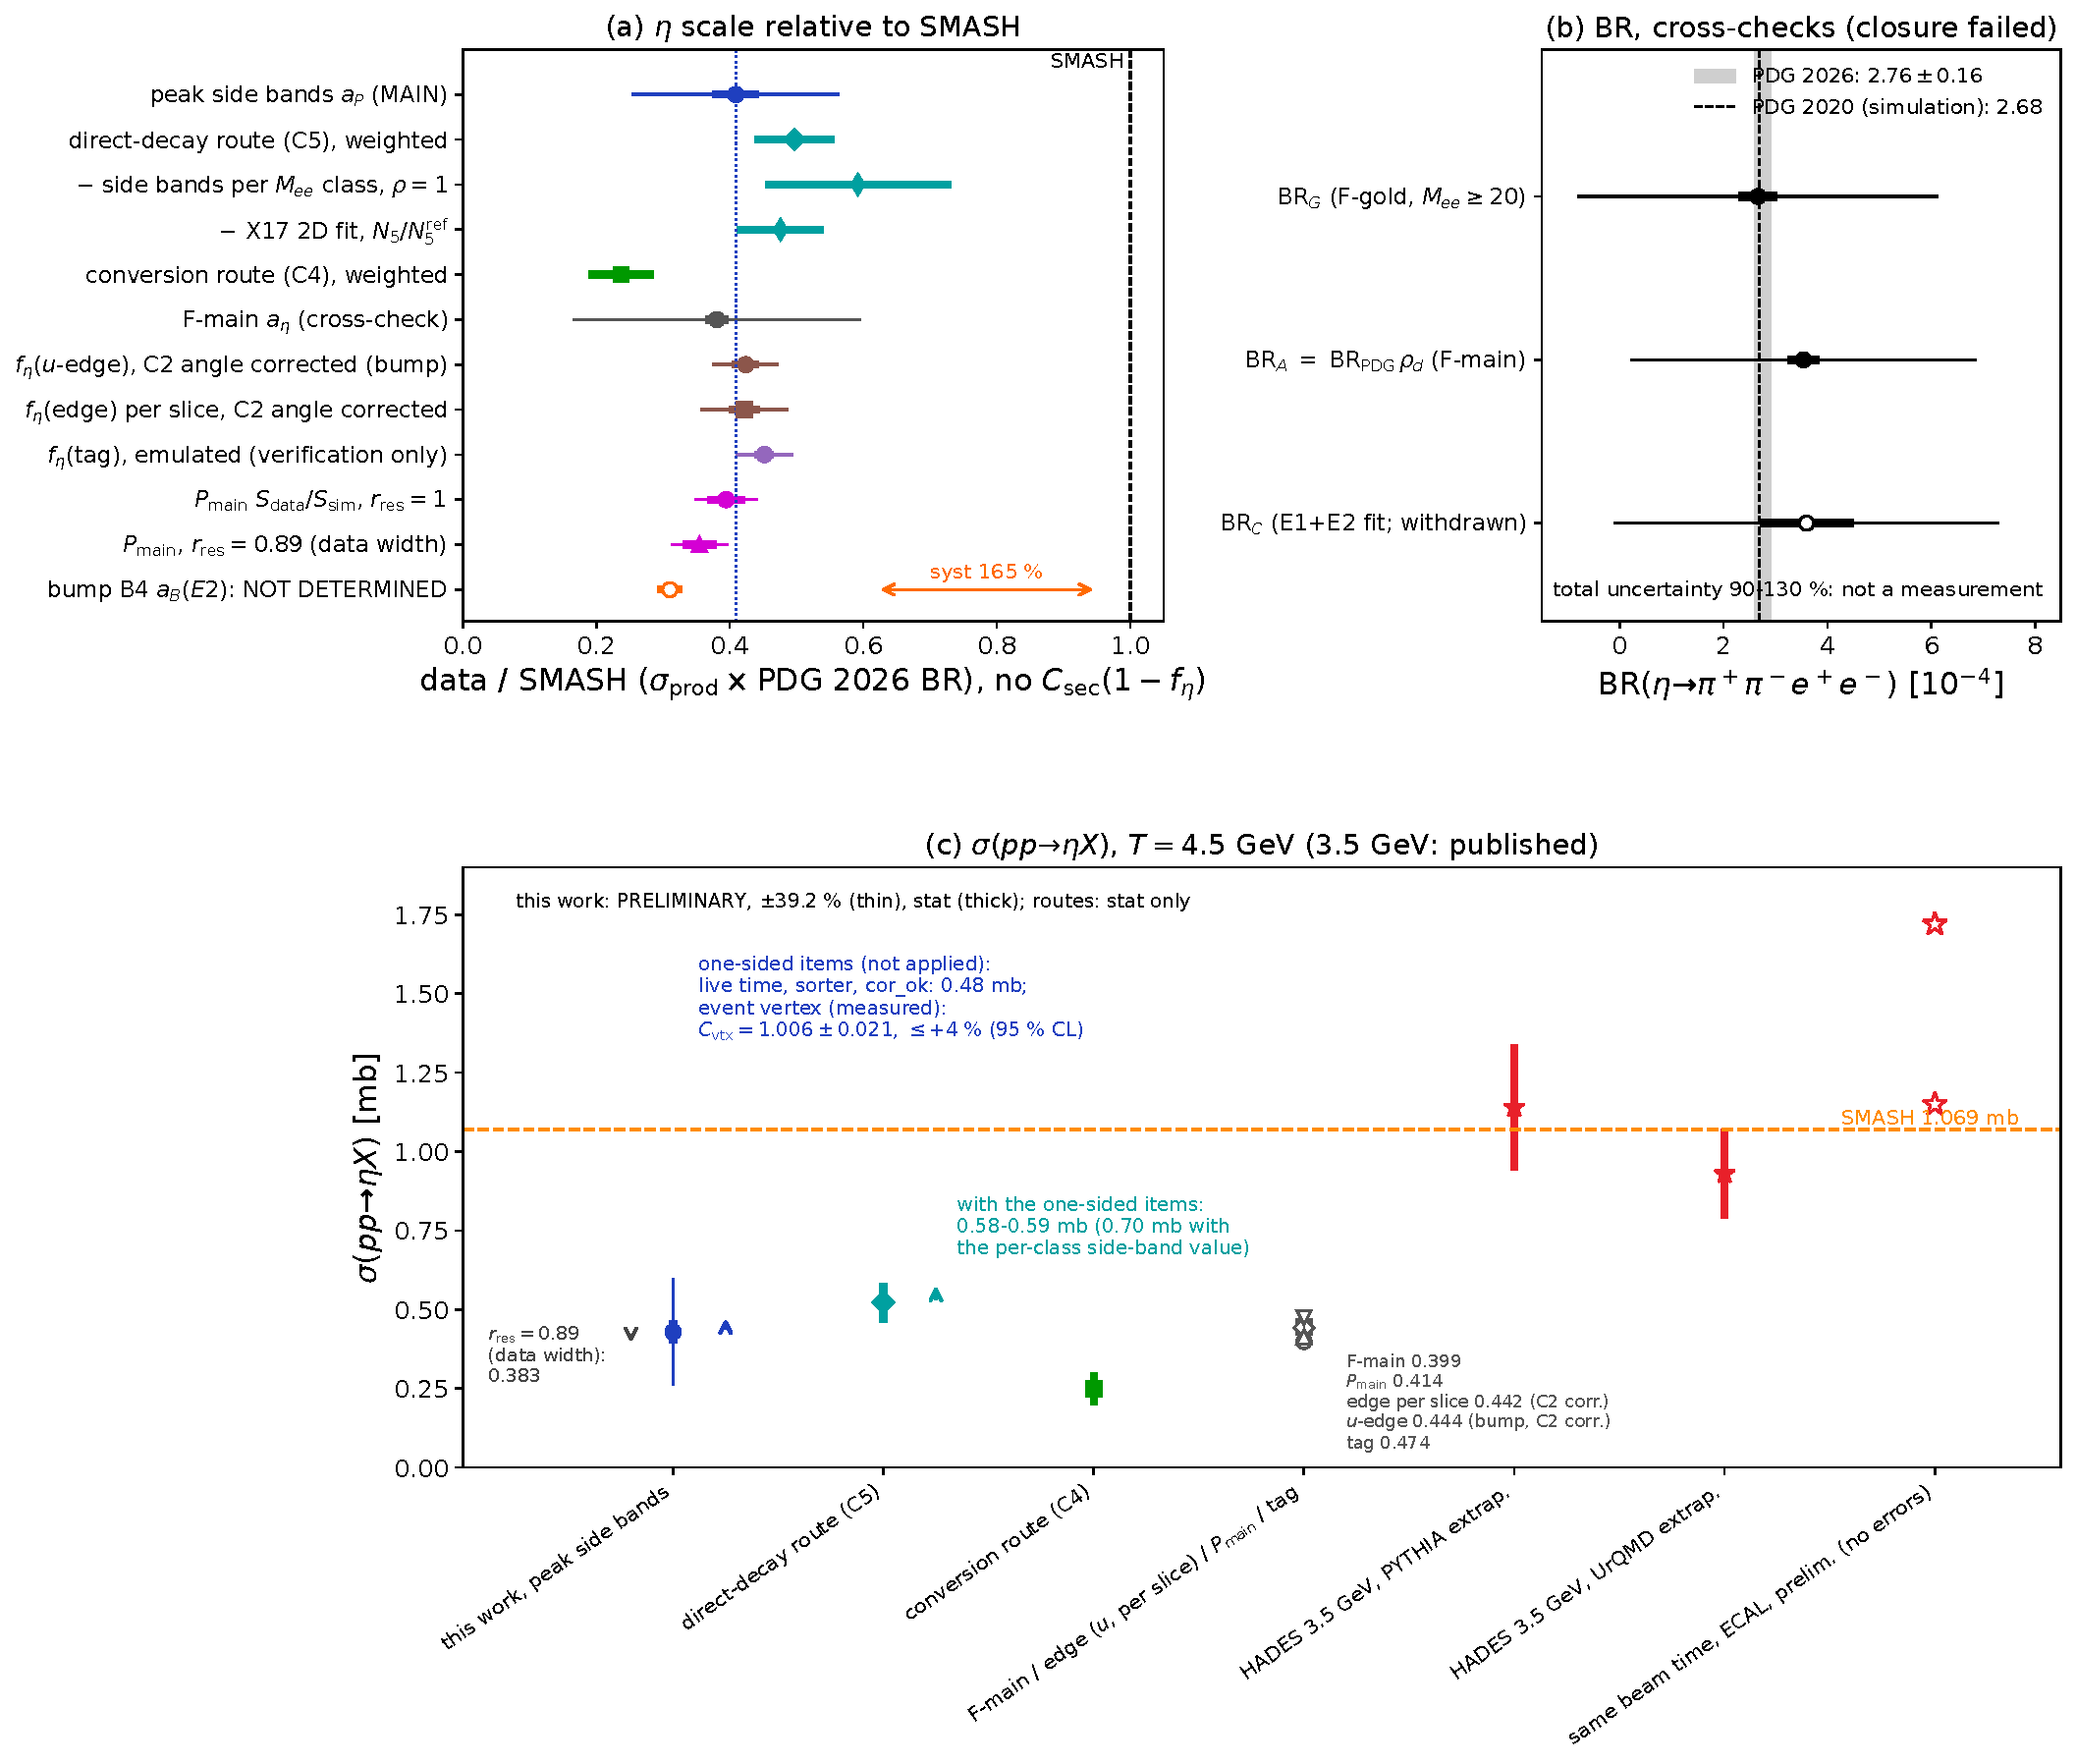
\includegraphics[width=0.74\textwidth]{figs_all/fix2_P1abc_v4.pdf}\\[0.2em]
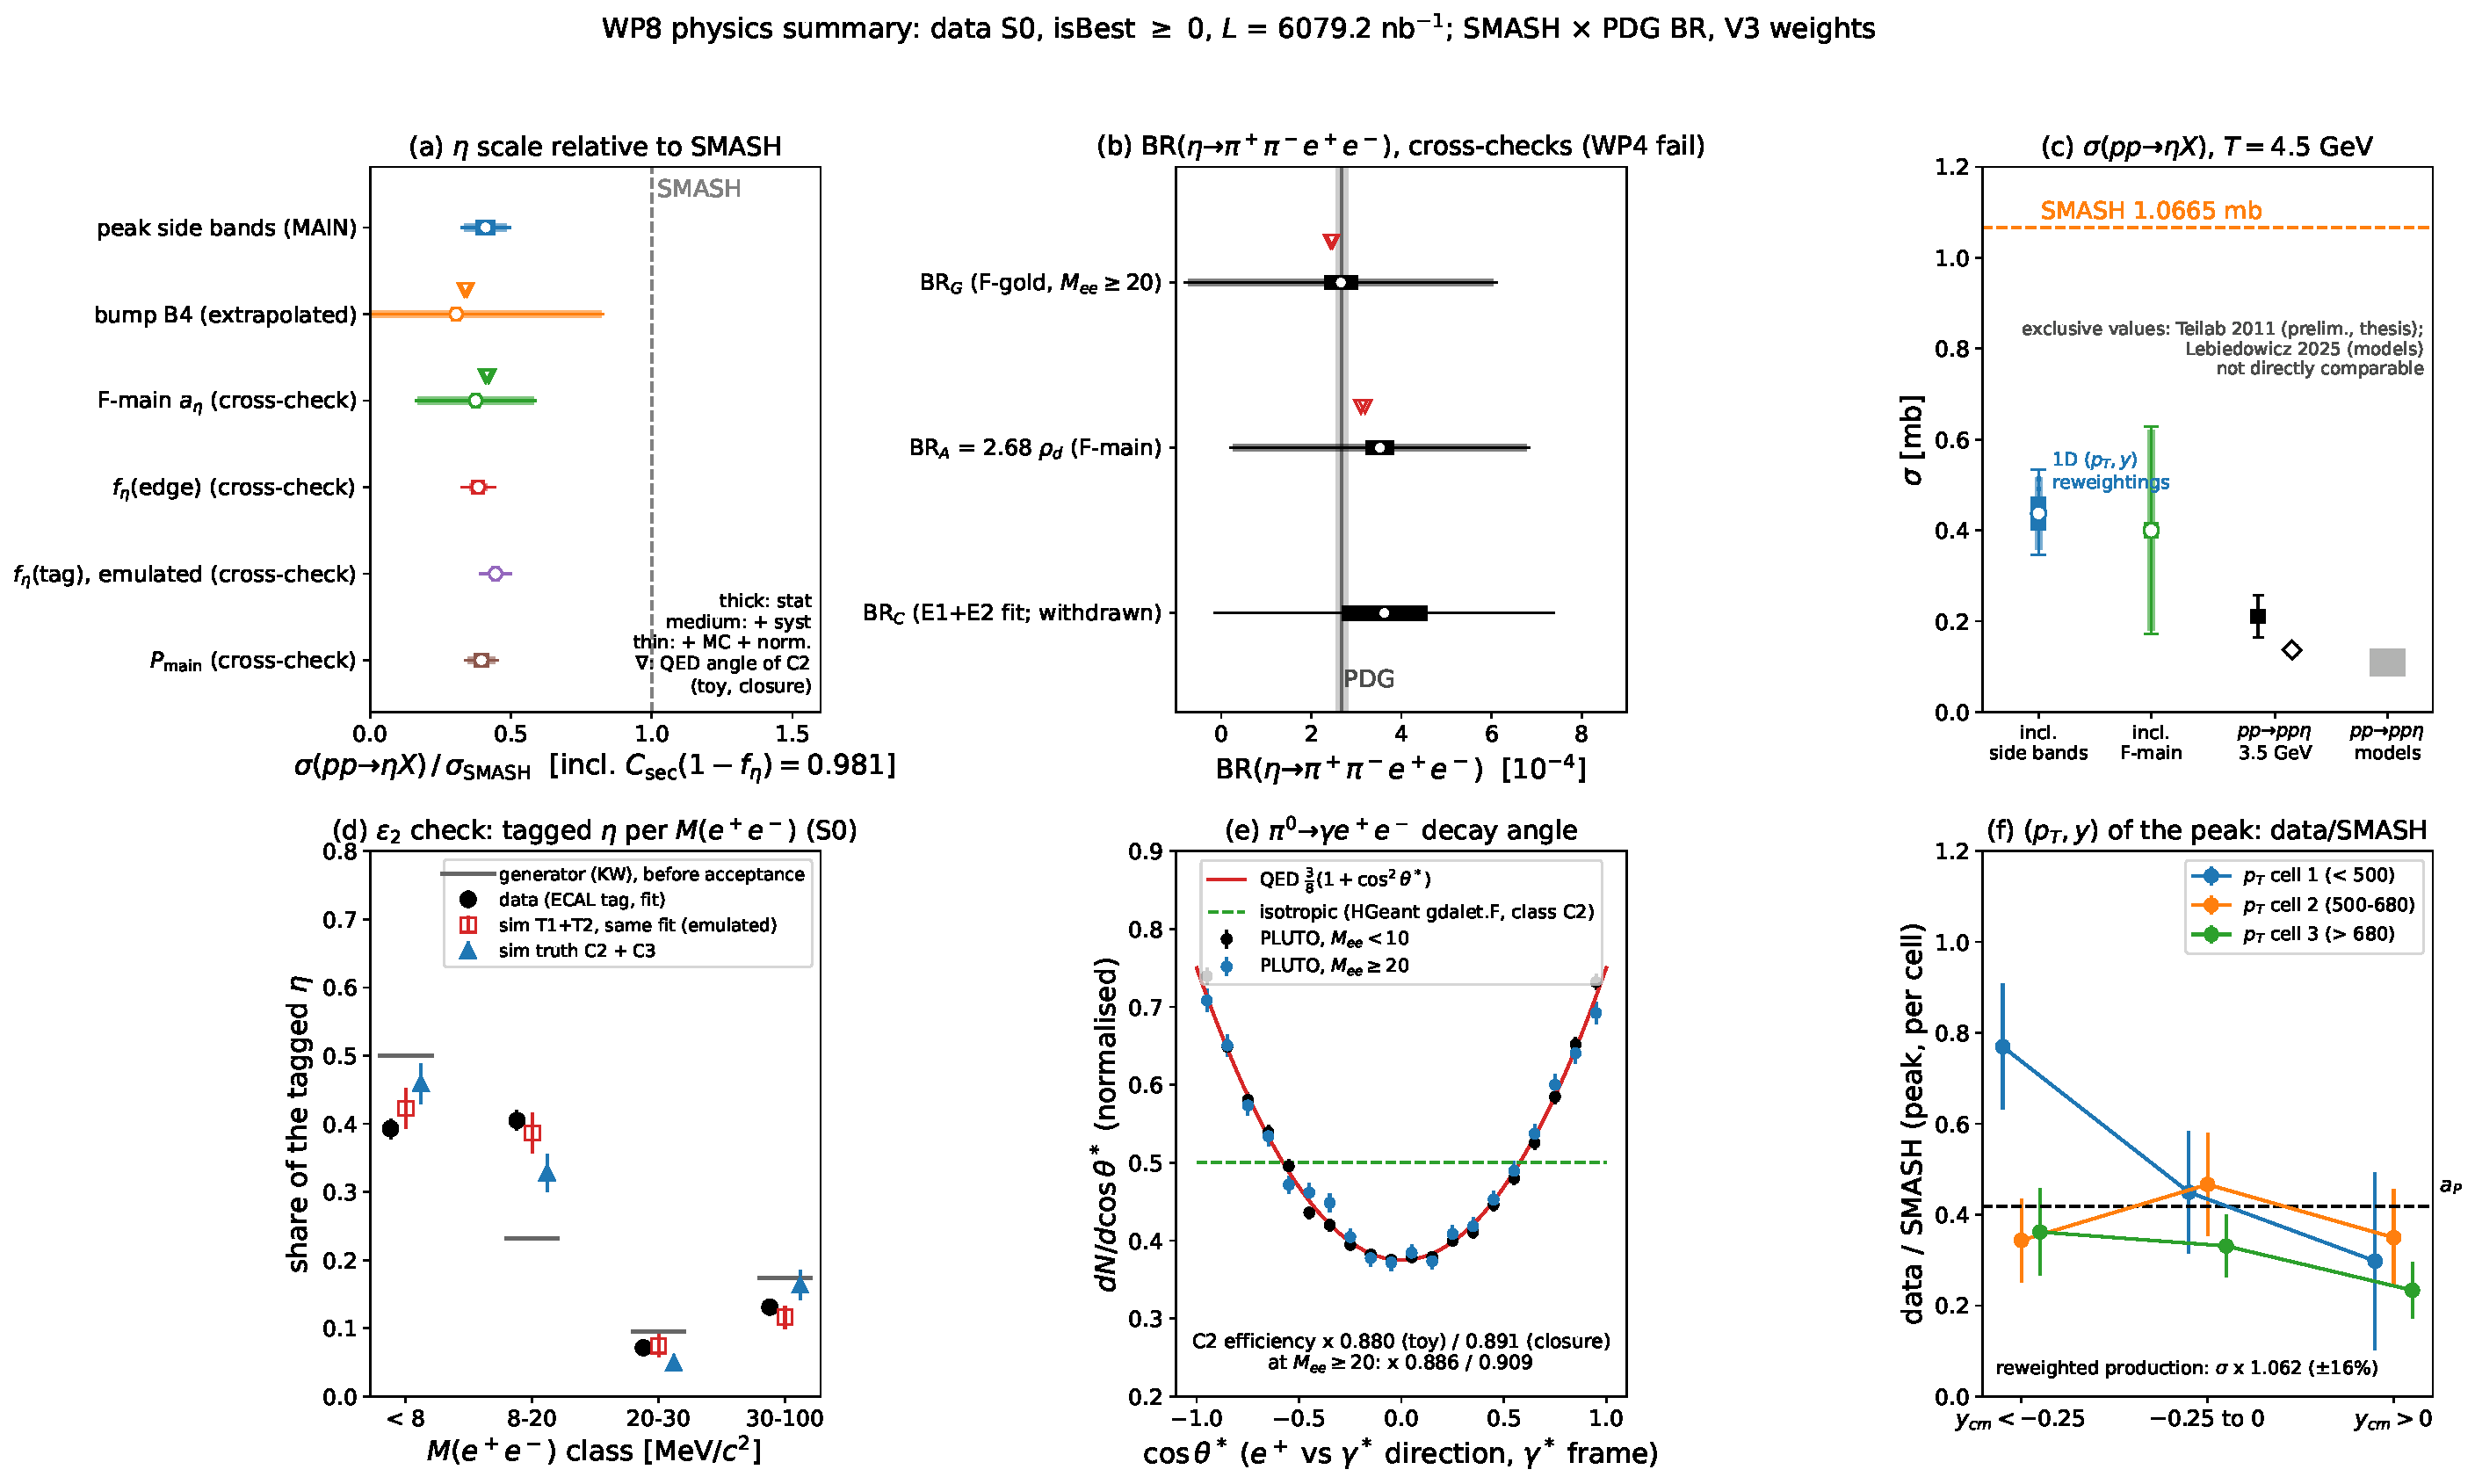
\includegraphics[width=0.90\textwidth,trim=0 0 0 442,clip]{figs_all/wp8_P1.pdf}
\caption{Spec.\ Fig.~P1: summary of the physics quantities.
Selection: data S0 (PT3 trigger, event vertex at $\vz>-160$\,mm, \betanew identification, corrected momenta, isBest $\ge0$, both pions in the event-vertex fit), each estimate with its own windows (peak side bands: peak window 0.53364--0.55416, side bands 0.5250--0.5336 and 0.5542--0.5628\,\GeVcc; F-main, F-gold: \Mee$\ge10$, $\ge20$\,\MeVcc, \Mfour 0.400--0.700\,\GeVcc; bump edges: \Mpipi 0.30--0.40\,\GeVcc); (d) ECAL-tagged counts in \Mee $<8$, 8--20, 20--30, 30--100\,\MeVcc; (e) generator level, no cut; (f) $3\times3$ cells of $p_T$ ($<500$, 500--680, $>680$\,\MeVc) and c.m.\ rapidity ($<-0.25$, $-0.25$--0, $>0$). Data S0, isBest $\ge0$, $L=6079.2\,\nbinv$; SMASH $\times$ PDG BR, V3 weights,
$M_4'=0.99615\,M_4$. Top row (redrawn in the review, \code{fix_figs.py}, PDG 2026, revised errors; panel (c) redrawn after the vertex study,
(a) and (c) with the C2-corrected bump edges, \code{fix2_P1abc_v4.py}): (a) $\eta$ scale data/SMASH per estimator and per route (direct
decays, conversions) and of the bump edges, in $u$ and per slice (PDG 2026: 0.424 and 0.422 for the 0.426 and 0.423 of the text); thick: stat, thin: total, the total of the side bands
including the composition of the peak; B4 not determined. (b) BR$(\eta\to\ppee)$ from F-gold, F-main and F-free (cross-checks, closure failed) against PDG 2026 (band) and PDG 2020 (dashed).
(c) \sigeta: this work (PRELIMINARY; thin: total 39.2\,\%, with the peak tail of D40), the two routes, the cross-checks, the one-sided items (arrows: live
time, sorter, \code{cor_ok} on the adopted value, 0.48\,mb, and on the weighted direct-decay route, 0.58--0.59\,mb, 0.70\,mb with its per-class
side-band value; the measured vertex factor
$C_{\mathrm{vtx}}$ adds at most 4\,\%), the
published inclusive HADES values at 3.5\,GeV and the unpublished same-beam-time ECAL values (open stars, no errors). Bottom row (WP8,
\code{wp8_P1.pdf}, unchanged): (d) eps2 check: share of the ECAL-tagged $\eta$ per \Mee class: data (fit), emulated simulated tag (same fit),
simulated truth C2+C3, generator fraction before acceptance. (e) Decay angle of $\piz\to\gamma\ee$ in PLUTO (lepton set, 124\,k decays) against
QED $(3/8)(1+\cos^2\theta^*)$ and the isotropic decay of HGeant (class C2). (f) Data/SMASH of the peak yield in $3\times3$ $(p_T,y)$ cells.
Fall-backs: template fits demoted, bump extrapolated, \sigeta PRELIMINARY.}
\label{fig:P1}
\end{figure}

%======================================================================
\section{The \texorpdfstring{$\eta$}{eta} bump through its kinematic edge}
\label{sec:bedge}
%======================================================================
\inshort{Cross-check of the $u$-edge (\S\ref{sec:edgeu}; D37, approved: $u$ is the bump measurement, this edge the cross-check). Part~II's edge step is turned into a measurement of the bump. The step at the kinematic edge of $\eta\to\pipi\piz$ is
$0.423\pm0.023\,(\mathrm{stat})\pm0.038\,(\mathrm{syst})\pm0.048\,(\mathrm{MC})$ of SMASH with the C2 decay angle corrected by per-count QED
weights (D35, D38) and $0.392\pm0.021\pm0.035\pm0.042$ in the frozen convention (both with the peak-tail family of D40); the visible yield in the
bump window is $21\,445\pm1152\pm1900\pm2223$ counts and the bump alone gives $\sigeta=0.442$\,mb (0.409\,mb uncorrected). The estimator recovers the truth of pseudo-data within 2\,\% and is
almost blind to the smooth background terms that defeat B4; it is simulation-limited (MC error twice the statistical one) and determined to
15--20\,\%. Only the background-subtracted area of the bump (B4) stays not determined.}

\begin{table}[H]
\centering
\caption{\textbf{What it shows: the three readings of the bump edge and what follows from them.} S0, isBest $\ge0$, $L=6079.2\,\nbinv$, all
\Mee; yields are raw counts $\times64/63$ in the bump window B (0.4550--0.5225\,\GeVcc). Errors: stat (200 bootstrap copies of the data), syst
(families E1--E10, Table~\ref{tab:bedge-syst}), MC (rms over the 100 simulation replicas) and, for \sigeta, the normalisation ($L$ 6.9\,\%,
period 5\,\%, BR$(\eta\to\pipi\piz)\times$BR$(\piz\to\gamma\ee)$ 3.17\,\%, $\Csec(1-\feta)$ $^{+3.1}_{-4.1}$\,\%). \sigeta $=$ scale $/1.00436$
(PDG 2026) $\times1.0694$\,mb $\times1.0104\times0.97$. $Y/L$ carries in addition $L\oplus$ period (8.5\,\%). Source: \code{tables_all/bedge_results_v3.txt} (C2 angle with
per-count QED weights, D38; peak-tail family E10, D40), earlier version verified by vbedge.}
\label{tab:bedge-res}
\footnotesize
\setlength{\tabcolsep}{2pt}
\begin{tabularx}{\textwidth}{@{}>{\raggedright\arraybackslash}p{2.4cm} L L L@{}}
\toprule
quantity & SMASH as is ($\kappa=1$), frozen convention & C2 angle corrected (per-count weights, D35, D38) & C2 corrected, conversions $\times0.48$ \\
\midrule
$\eta$ scale of the bump, $f_\eta(\mathrm{edge})$ & $0.392\pm0.021\pm0.035\pm0.042$ & $\mathbf{0.423\pm0.023\pm0.038\pm0.048}$ & $0.569\pm0.031\pm0.071\pm0.084$ \\
total (stat $\oplus$ syst $\oplus$ MC) & 15.0\,\% & 15.4\,\% & 20.0\,\% \\
the same with PDG 2026 BRs & 0.390 & 0.422 & 0.567 \\
\Ybump(B, all \Mee) [counts] & $21\,445\pm1152\pm1900\pm2223$ & $21\,353\pm1147\pm1919\pm2322$ & $21\,744\pm1168\pm2700\pm3071$ \\
$Y/L$ [visible counts per \nbinv] & $3.53\pm0.19\pm0.31\pm0.37$ & $3.51\pm0.19\pm0.32\pm0.38$ & $3.58\pm0.19\pm0.44\pm0.51$ \\
\sigeta [mb] & $0.409\pm0.022\pm0.036\pm0.044$ $^{+0.039}_{-0.041}$ & $\mathbf{0.442\pm0.024\pm0.040\pm0.050}$ $^{+0.042}_{-0.044}$ & $0.594\pm0.032\pm0.074\pm0.087$ $^{+0.057}_{-0.059}$ \\
total of \sigeta, without / with norm. & 0.061 / 0.073\,mb (18\,\%) & 0.068 / 0.081\,mb (18\,\%) & 0.119 / 0.132\,mb (22\,\%) \\
\bottomrule
\end{tabularx}
\end{table}

\subsection{The procedure in plain words}
\label{sec:bedge-proc}
\begin{enumerate}\setlength{\itemsep}{1pt}
\item \textbf{What makes the edge.} In $\eta\to\pipi\piz$ with $\piz\to\gamma\ee$ (C2) or a converted \piz photon (C3) one photon is lost. The
      four tracks then carry less mass than the $\eta$, but at most $M_4^{\max}(\Mpipi)$, a limit set by kinematics alone. Summed over the
      events this gives a broad bump that ends in a sharp step. The step sits at $0.99277\,M_4^{\max}(\Mpipi/0.9970)$ on the data scale (the
      factors are frozen from Part~II); its position is fixed, not fitted.
\item \textbf{The fit.} In each of the four \Mpipi slices 0.30--0.34, 0.34--0.37, 0.37--0.39 and 0.39--0.40\,\GeVcc, $N-\mathrm{CB}$ per 2.5\,\MeVcc
      is fitted with a second-order polynomial [+ the $\eta$ peak as a Gaussian, 0.5439 / 5.4\,\MeVcc] plus $h$ times a step smeared by
      5.4\,\MeVcc. The \emph{same} fit, with the same fixed covariance, is applied to the simulated $T_1+T_2$ (SMASH at $\sigma\times$PDG BR,
      $w\times$V3, expected raw counts). $E$ is the sum of the four heights, and $f_\eta(\mathrm{edge})=E_{\mathrm{data}}/E_{\mathrm{sim}}$. WP6's
      numbers are reproduced to all digits: $E_{\mathrm{data}}=1141.86\pm59.22$, $E_{\mathrm{sim}}=2915.70$, $f_\eta(\mathrm{edge})=0.39162$.
\item \textbf{Counts and templates.} Data: the S0 counts (\code{cor_ok}), $N$, $N_{++}$, $N_{--}$ per \Mee class (E1, E2), 5\,\MeVcc \Mpipi bin and
      2.5\,\MeVcc \Mfour bin; the CB is rebuilt per slice exactly as in the histogram factory. Simulation: std + lep + $\eta$ sets, owned entries,
      nine groups (C2, C3, C4, C5, \Geta, $G_D$ and $G_C$ each split into $\omega/\rho^0$ pions and the rest), 15 configurations for the variants.
\item \textbf{Errors.} Stat: rms over 200 bootstrap copies of the data (Poisson(1) weight per event group; $E_{\mathrm{sim}}$ fixed). MC: rms over
      the 100 simulation replicas ($E_{\mathrm{data}}$ fixed). For every variant both sets are rerun, so the noise of every shift is measured.
\item \textbf{Systematics.} 43 variants in seven families (E1 edge model, E2 slices, E3 mass transfer and resolution, E4 CB, E5 physics weights,
      E6 selection, E7 step of a smooth background), plus E8 (C2 factor) and E9 ($\kappa$ of the peak) for the corrected readings, and E10 (the low-mass tail of the peak, $t=1\pm0.5$, D40) for
      all readings (the package names its families E1--E10, as in Fig.~\ref{fig:bedge-syst}a, which shows E1--E9; they are not the \Mee classes
      E1, E2). The Part~III
      rules of WP7 are used: a shift counts as $\delta^2=\max(0,\Delta^2-|\sigma^2_{\mathrm{stat},v}-\sigma^2_{\mathrm{stat},0}|-\mathrm{MC}(\Delta)^2)$;
      a pair of opposite variants counts $(|\delta_+|+|\delta_-|)/2$; a family is its largest entry; families add in quadrature; variants that
      the data reject are listed, not counted (rule R1).
\item \textbf{C2 decay angle} (\S\ref{sec:bedge-c2}): $f_{\mathrm{corr}}=E_{\mathrm{data}}/[E_{\mathrm{sim}}(1-\sum_i(1-c_i)\,\mathrm{C2}_i/T_{12})]$ per \Mee
      class $i$. D35 used the constant factor $c=0.8855$ (all \Mee; 0.879 / 0.882 for E1 / E2), the mean of the WP8 toy and closure; since D38
      (approved) $c_i$ are the per-count QED weights averaged in each class (0.868 / 0.854 for E1 / E2, effective 0.860; \S\ref{sec:c2recon}). The C2 share of the
      simulated step comes from fitting the simulation once more with the data covariance, which makes $h$ a linear function of the spectrum:
      C2 53.6\,\%, C3 45.3\,\%, rest 1.1\,\% (E1: 37.8 / 58.7\,\%; E2: 78.1 / 25.3\,\%).
\item \textbf{Conversion scale $\kappa$.} (a) $\kappa=0.48\pm0.11$ imported from the peak (conversion route / direct-decay route $=0.237/0.497$):
      $a=E_{\mathrm{data}}/[E_{\mathrm{sim}}(c\,s_{\mathrm{C2}}+0.48\,s_{\mathrm{C3}}+s_{\mathrm{rest}})]$; (b) $\kappa$ free, E1 and E2 solved together.
\item \textbf{Yields and \sigeta.} $\Ybump(\mathrm{edge})=f_\eta\times(\mathrm{C2}+\mathrm{C3})_{\mathrm{B}}$, with SMASH's 54\,758.9 counts in B: the scale
      is measured at the edge and carried over the window with the simulated shape of the bump. \sigeta as in Table~\ref{tab:bedge-res};
      $\mathrm{DR}_{\mathrm{edge}}=\aP/f_\eta(\mathrm{edge})$, both with PDG 2026.
\item \textbf{Pseudo-data} (\S\ref{sec:bedge-toys}): 16 truths $\times$ 1000 toys with the WP4 machinery.
\end{enumerate}

\textbf{Further numbers} (all \Mee unless stated). By class: $f_\eta(E1)=0.367\pm0.022\pm0.043\pm0.050$, $f_\eta(E2)=0.431\pm0.041\pm0.051\pm0.084$ (C2
corrected 0.386 and 0.487; they differ by 0.5--0.7$\sigma$). Yields: B, E1 $10\,876\pm652\pm964\pm1413$; B, E2 $10\,826\pm1028\pm959\pm1949$; whole
\Mfour range $26\,959\pm1449\pm2388\pm2816$ counts (4.435 per \nbinv). In \Mee$\ge10$\,\MeVcc the edge gives $10\,830\pm2400$ counts, where B4 gives
7822 with a linear and 19\,526 with a quadratic background, and WP6's interpolation to a closed CR-L about 12\,900 (\S\ref{sec:closure}). All
\Mee: B4 16\,389 (not determined), F-main $19\,426\pm2478$ (cross-check). $\kappa$ free: $a_D=0.574\pm0.088\,(\mathrm{stat})\pm0.235\,(\mathrm{MC})$,
$\kappa=0.470\pm0.242\pm0.465$ (robust MC; the replica distribution has long tails, rms 11.7 for $a_D$, so this is not a measurement);
uncorrected with $\kappa=0.48$: 0.513.

\subsection{Systematic uncertainties}
\label{sec:bedge-syst}

\begin{table}[H]
\centering
\caption{\textbf{What it shows: no systematic family exceeds 7\,\% of the edge scale; the simulation statistics (MC) are larger than all of
them together.} Families in per cent of the value (WP7 rules). Family E5 does not count the phase-space and weights-off Dalitz-plot variants (see
text); counted, the total of $f_\eta(\mathrm{edge})$ would be 11.3\,\%. Family E7 is a symmetric envelope of unknown sign. E8 is the model
allowance of the per-count C2 weights (D38), E10 the peak-tail family of D40. Source: \code{tables_all/bedge_syst_v3.txt} (every variant).}
\label{tab:bedge-syst}
\footnotesize
\begin{tabular}{@{}l r r r@{}}
\toprule
family & $f_\eta(\mathrm{edge})$ & C2 corrected & C2 corr., $\kappa=0.48$ \\
\midrule
E1 edge model & 1.1 & 1.4 & 0 \\
E2 \Mpipi slices & 2.9 & 2.9 & 3.8 \\
E3 mass transfer, resolution & 4.3 & 4.3 & 4.4 \\
E4 CB & 1.3 & 1.3 & 1.3 \\
E5 physics weights & 1.2 & 1.2 & 1.1 \\
E6 selection & 0 & 0 & 2.1 \\
E7 step of a smooth background & 6.0 & 6.0 & 6.0 \\
E8 C2 factor, model ($\pm0.004$, D38) & -- & 0.2 & 0.3 \\
E9 $\kappa$ of the peak ($\pm0.11$) & -- & -- & 7.2 \\
E10 peak tail, $t=1\pm0.5$ (D40) & 3.4 & 3.7 & 4.9 \\
\midrule
total systematic & \textbf{8.9} & \textbf{9.0} & \textbf{12.4} \\
stat (bootstrap) & 5.4 & 5.4 & 5.4 \\
MC (replicas) & 10.9 & 11.3 & 14.7 \\
\bottomrule
\end{tabular}
\end{table}

\textbf{The counted variants.} The largest single entries: family E3, the simulated peak width of each sample used for its own smearing (data 5.4,
simulation 6.1\,\MeVcc), $-0.018$ (counted 0.0168), and the resolution factor $r_{\mathrm{res}}=0.89/1.10$ ($-0.022/+0.012$, pair 0.011); family E2, the
fit range starting at 0.29 ($+0.015$, counted 0.011); family E4, CB $=N_{++}+N_{--}$ ($+0.005$); family E5, the $\eta\to3\pi$ Dalitz plot $1+aY$ ($-0.006$). A linear
background (family E1, pol1) is rejected by the data ($\chi^2$ 308.9/124 against 137.4/120) and not counted; pol3 stays within its noise.

\textbf{Two Dalitz-plot variants are not counted.} ``Physics weights off'' and ``phase-space Dalitz plot'' move $f_\eta(\mathrm{edge})$ by $+0.034$ and
$+0.032$. The bump package rejected them with the per-slice pattern of $h_{\mathrm{data}}/h_{\mathrm{sim}}$, $\chi^2=67/3$ and $65/3$ against $4.5/3$
for the nominal. That test used the data errors only; with the template errors of the simulated steps (13--43\,\% per slice) the verifier finds
$14.8/3$ ($p=0.002$) against $1.2/3$: still disfavoured ($\Delta\chi^2=13.6$), but the exclusion rests on the KLOE-2 measurement of the
$\eta\to3\pi$ Dalitz plot and on the rule R1 of WP7 (F-main: $\Delta\chi^2=38>25$). Counted, family E5 would be 0.028--0.030 and the systematic error
11.3\,\% instead of 8.9\,\% (total 16.6 instead of 15.0\,\%; both with the peak-tail family E10).

\textbf{Family E7, the step of a smooth background.} The step template is odd around the edge, so the odd (cubic) part of a smooth background that the
second-order polynomial cannot absorb projects onto $h$. The non-$\eta$ background, smoothed with exp(pol3) and projected with the data
covariance, gives $K=-52.3$ counts (1.8\,\% of the bump step), i.e.\ a bias of $-0.004$ to $-0.011$ for a SMASH-like and $-0.023$ for a
stage-A-like background. The verifier shows that the sign depends on the smoother: exp(pol2), exp(pol4) and exp(pol5) give $K=-16.6$, $-15.9$ and
$+48.6$ counts and a stage-A-like bias of $-0.010$, $-0.005$ and $+0.030$. Family E7 is therefore an uncertainty of unknown sign, counted as a symmetric
envelope of 0.0234 (6.0\,\%); exp(pol5) would give 7.5\,\% (systematic 10.0\,\%).

\textbf{Statistical and MC errors.} The bootstrap gives 0.021 (1.04 times the fit error; the verifier 0.99 times); the factor 1.2 of the Part~II
calibration (40 random halvings of ``pre'') is not confirmed and not used (with it the error would be 0.024). The MC error is the replica rms of
the ratio, 0.042 (WP6's linear estimate 0.039, the robust 68\,\% width 0.033); the pseudo-data need the rms for coverage. An independent replica
set gives 0.038, within the 7--10\,\% sampling error of a 100-replica rms, so the quoted value is on the high side. Half to 57\,\% of the MC variance
of $E_{\mathrm{sim}}$ comes from the raw non-bump part of the simulation (its step projection is $+32$ counts with a replica rms of 190--217). The
replica mean of $f_\eta$ lies $+2.4$\,\% above the nominal with the WP0 replicas but only $+0.8$\,\% with the verifier's independent set (the plain
$1/E_{\mathrm{sim}}$ effect, 0.9\,\%): the WP0 set's mean $E_{\mathrm{sim}}$ is 1.3$\sigma$ low. The template-statistics correction of $f_\eta$ is
therefore about $-1$\,\%, not the $-2.4$\,\% first quoted; information only, not applied.

\begin{figure}[!htbp]
\centering
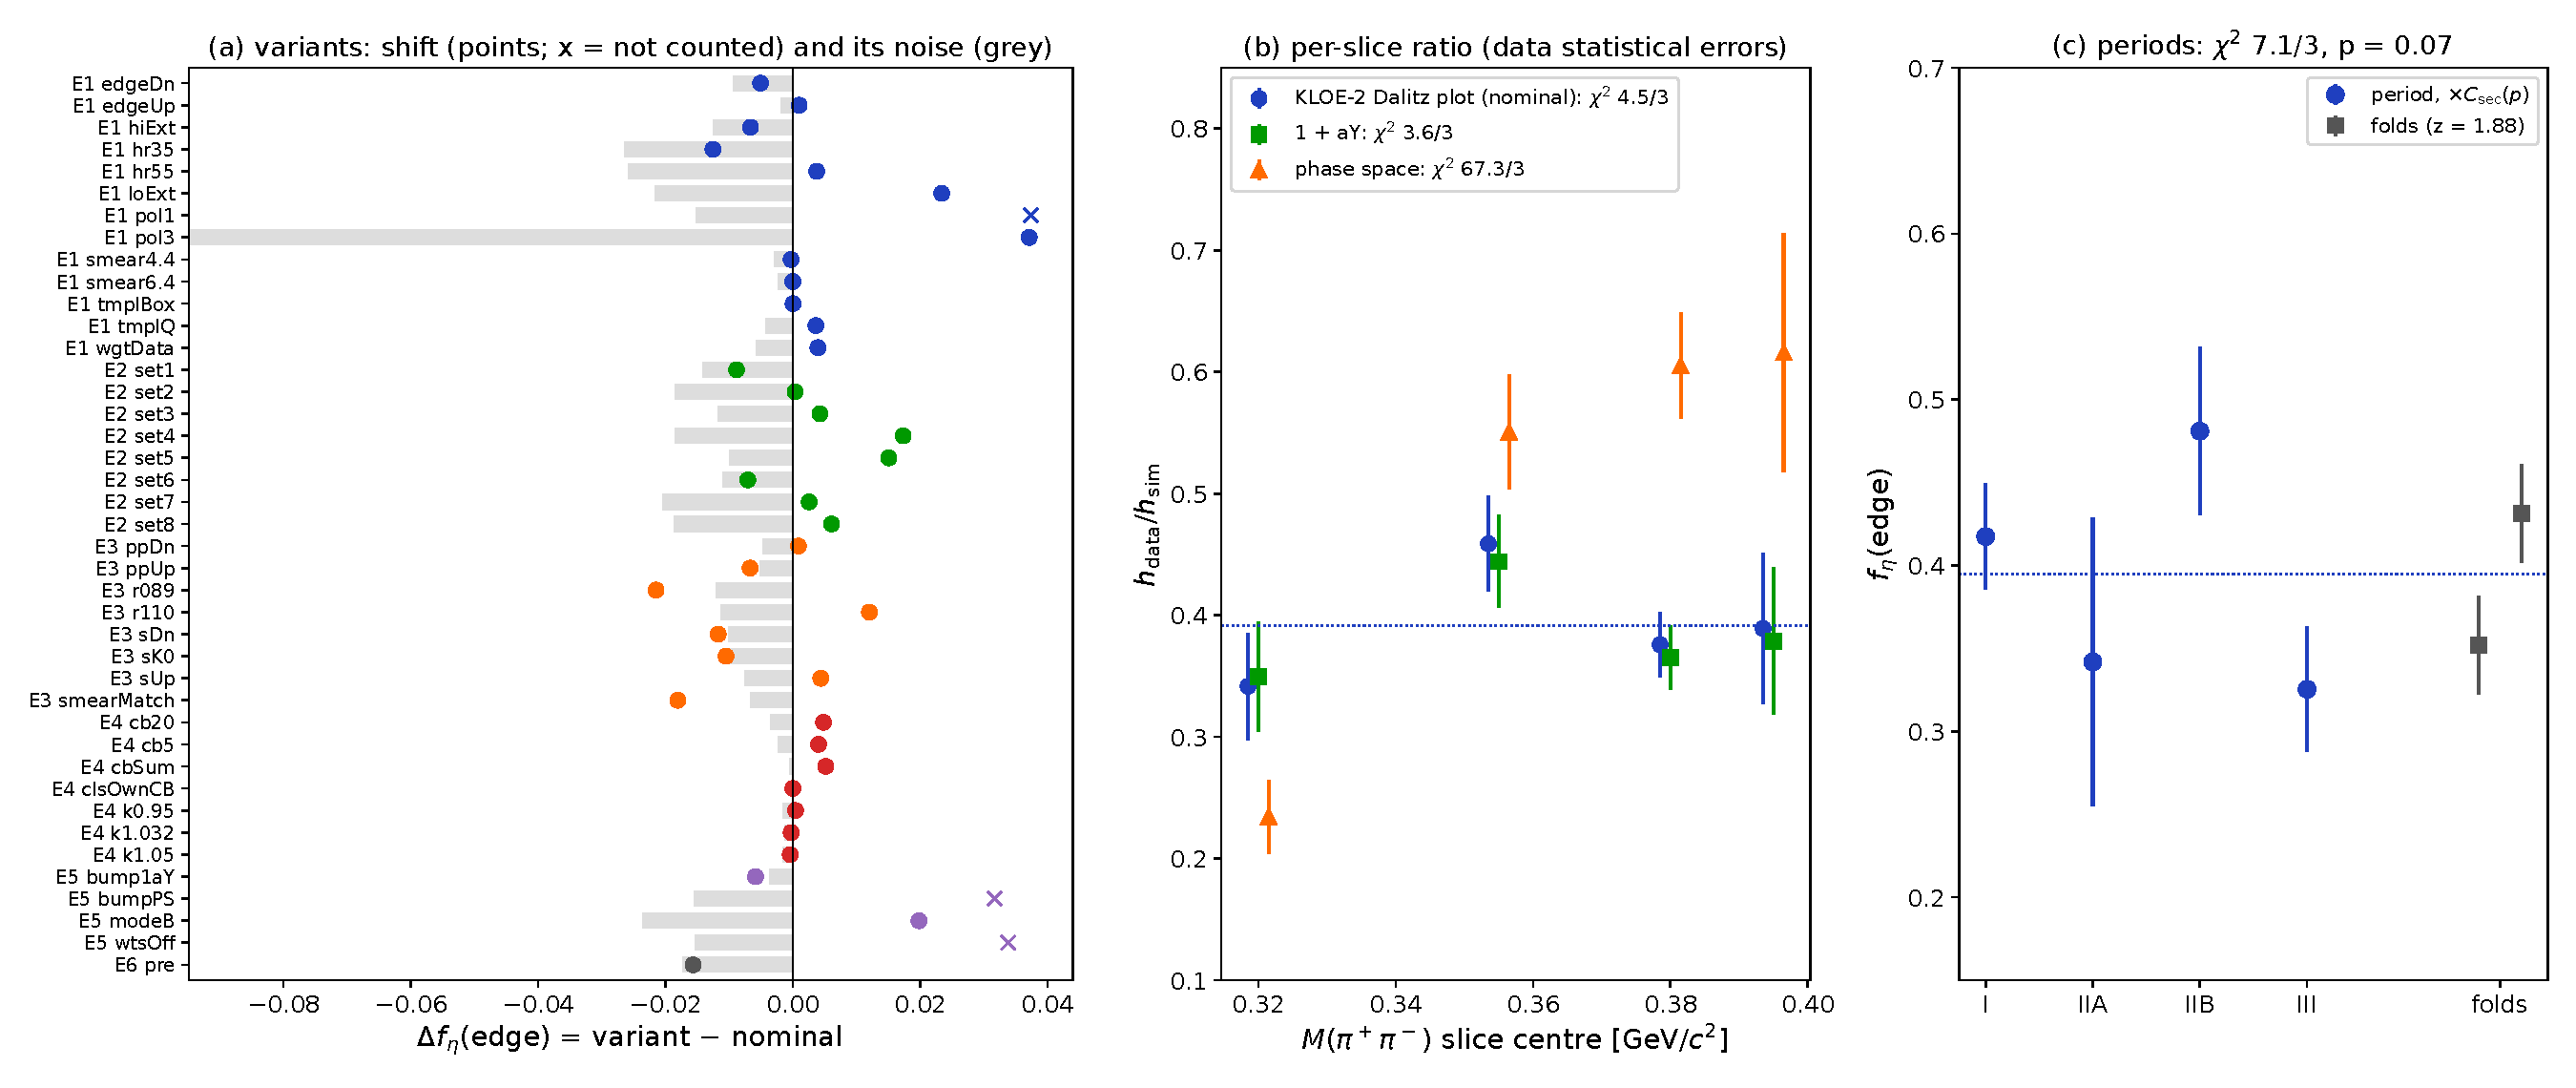
\includegraphics[width=\textwidth]{figs_all/bedge_syst.pdf}
\caption{\textbf{What it shows: no variant moves $f_\eta(\mathrm{edge})$ by more than its noise except the resolution ($r_{\mathrm{res}}$) and the
Dalitz-plot variants that are not counted; the periods and the two folds agree within their errors (the folds marginally).}
Selection: data, S0 (PT3 trigger, event vertex in the target region ($\vz>-160$\,mm), \betanew particle identification (pions within $3\sigma$, leptons within $5\sigma$ and with a RICH ring), energy-loss-corrected momenta of all four tracks, all stored combinations of each event (isBest $\ge0$), both pions in the event-vertex fit), all \Mee, in the \Mpipi slices 0.30--0.34, 0.34--0.37, 0.37--0.39, 0.39--0.40\,\GeVcc; 2.5\,\MeVcc bins, fit range the edge $\pm45$\,\MeVcc ($\pm35$\,\MeVcc in 0.39--0.40), step smeared by 5.4\,\MeVcc; CB $=2\sqrt{N_{++}N_{--}}$ of each slice in 10\,\MeVcc cells, $k=1$; simulation $T_1+T_2$ of SMASH p+p at 4.5\,GeV (standard, lepton and $\eta$ sets, mode A) at its cross sections $\times$ PDG BR $\times$ the $\eta$-decay weights V3, masses moved to the data scale ($M_4'=0.99615\,M_4$, $\Mpipi'=0.9952\,\Mpipi$), same cuts, same fit. (a) each variant changes one item (family E6: ``pre'' in data and simulation). (b) KLOE-2, $1+aY$ and phase-space Dalitz plots of $\eta\to\pipi\piz$ in the simulation. (c) periods days 034--046, 047--048, 049--053, 059--067 (simulation $\times L_p/L$); folds: the two halves of the data by event-group parity.
Data S0, $f_\eta(\mathrm{edge})$ without the C2 correction. (a) Shift of every variant from the nominal (points; crosses: not counted) and the noise
of the shift (grey bars, literal Part~III rule); colours mark the families E1 (blue), E2 (green), E3 (orange), E4 (red), E5 (violet) and E6 (grey).
(b) Per-slice $h_{\mathrm{data}}/h_{\mathrm{sim}}$ for the KLOE-2 (nominal), $1+aY$ and phase-space Dalitz plots, with the data statistical errors only;
the $\chi^2$ values of the legend leave out the template errors of the simulated steps (with them: 1.2/3 nominal, 14.8/3 phase space). Dotted: the
nominal $f_\eta(\mathrm{edge})$. (c) Per-period $f_\eta(\mathrm{edge})\times\Csec(p)$ ($\chi^2=7.1/3$, $p=0.07$) and the two folds ($z=1.88$; 1.9--2.0 with
other error scalings, $p\approx0.05$, marginal).}
\label{fig:bedge-syst}
\end{figure}

\subsection{Consistency tests}
\label{sec:bedge-tests}
\begin{itemize}\setlength{\itemsep}{1pt}
\item \textbf{Periods} (data of a period against the simulation $\times L_p/L$): raw 0.408, 0.342, 0.481, 0.325 for I, IIA, IIB, III ($\chi^2=6.77/3$,
      $p=0.080$); $\times\Csec(p)$: $0.417\pm0.032$, $0.342\pm0.087$, $0.481\pm0.051$, $0.325\pm0.038$ ($\chi^2=7.14/3$, $p=0.067$); C2 corrected
      $p=0.068$; class E1 $p=0.27$, class E2 $p=0.047$--0.050 (marginal). The WP7 rule adds a term only for $p<0.01$: none added. IIB high and III low
      repeat the pattern of the vertex hint of Part~II; not significant.
\item \textbf{Folds} (two halves of the data): $0.352\pm0.030$ and $0.431\pm0.030$, $z=1.88$ ($p=0.06$); the verifier finds $z=1.90$--1.99
      ($p=0.047$--0.057) depending on the error scaling: \emph{marginal}. No term is added.
\item \textbf{Selection}: ``pre''/S0 $=0.960$ ($z=-0.85$). isBest $=1$ in data and simulation: ratio 1.085 ($z=1.5$); isBest $=1$ in the data only
      (WP7 convention) 0.346, ratio 0.885, as WP7's \Ybump.
\item \textbf{Slices}: $h_{\mathrm{data}}/h_{\mathrm{sim}}=0.342$, 0.459, 0.376, 0.389 in the four slices: one scale describes them
      (Fig.~\ref{fig:bedge-syst}b).
\item \textbf{Control slices} (not in $E$): 0.40--0.41\,\GeVcc, data $18.7\pm14.7$ (simulation 116.2, the tail of the edge); 0.42--0.46\,\GeVcc,
      no bump, edge put at 0.515: data $15.4\pm15.0$, simulation $-14.5$. Without the bump the data show no step.
\end{itemize}

\subsection{Pseudo-data test}
\label{sec:bedge-toys}
The frozen estimator was run on 16 truths with 1000 pseudo-data sets each (WP4 machinery). Truth $=$ data CB $+\,c\times$ non-$\eta$ background
$\times(1+bx+qx^2)$ [$\times$ a local structure] $+$ the $\eta$ classes $\times$ their scales, with the raw or the smoothed simulated background;
each pseudo-data set has Poisson $N$ and like-sign counts, and its CB is rebuilt. The templates come either from the truth sample (AA: the
estimator alone) or from a bootstrap replica (RF: the realistic template noise).

\begin{table}[!htbp]
\centering
\caption{\textbf{What it shows: the edge estimator recovers the truth within 2\,\% for realistic backgrounds, also with the quadratic term that
moves B4 by $+150$\,\%; only a structure as narrow as the edge biases it.} Relative bias of $f_\eta(\mathrm{edge})$ in per cent (absolute for
$a=0$), pull width in brackets; 1000 pseudo-data sets per truth; $x=(\Mfour-0.55)/0.1$; $a$: $\eta$ scale of the truth. Source:
\code{tables_all/bedge_toys.txt}.}
\label{tab:bedge-toys}
\footnotesize
\setlength{\tabcolsep}{4pt}
\begin{tabularx}{\textwidth}{@{}L r r@{}}
\toprule
truth & AA (templates $=$ truth sample) & RF (templates $=$ replica) \\
\midrule
SMASH background $\times1$, $a=1$ (exact closure expected) & $-0.2$ (0.97) & $+2.2$ (1.15) \\
SMASH background $\times1$, $a=0.4$ & $+0.6$ (1.01) & $+3.0$ (1.13) \\
(a) WP4 scenario: background $\times1.35$, tilt $-0.15$, $a=0.4$ & $+1.6$ (1.02) & $+4.0$ (1.11) \\
(a) with $a=0$ (absolute bias of $f_\eta$) & $+0.017$ (0.98) & $+0.018$ (1.00) \\
\textbf{(a) + quadratic term $q=-0.173$ (moves B4 by $+150$\,\%)} & $\mathbf{-0.5}$ (1.01) & $+1.9$ (1.14) \\
(a) + $q=-0.346$ / $q=+0.173$ & $-2.5$ / $+3.8$ & $-0.2$ / $+6.3$ \\
WP4 (e): $\omega/\rho^0$-pion background $\times0.3$, rest $\times1.6$ & $-0.1$ (1.00) & $+2.4$ (1.15) \\
stage-A background with the F-main $\eta$ values & $+3.4$ (1.04) & $+5.9$ (1.10) \\
(a) with the smoothed background in the truth (a template-noise realisation) & $-7.8$ (0.96) & $-5.6$ (1.17) \\
(a) $\times\,(1+0.10\,G(0.490,\,15\,\MeVcc))$ & $+21.5$ (1.02) & $+24.4$ (0.97) \\
(a) $\times\,(1+0.05\,G(0.505,\,8\,\MeVcc))$ & $+10.7$ (0.94) & $+13.3$ (1.04) \\
truth at $s+0.0009$, $r_{\mathrm{res}}=0.89$ (the direction of family E3) & $+7.5$ (1.00) & $+10.1$ (1.06) \\
\midrule
\multicolumn{3}{@{}l}{\emph{matching estimators}} \\
truth C2 $\times0.8855$ $\to$ C2 corrected & $+1.9$ (1.02) & $+4.5$ (1.14) \\
truth conversions $\times0.48$ $\to$ $\kappa=0.48$ (uncorrected) & $+4.6$ (1.04) & $+7.3$ (1.03) \\
$a=0.55$, C2 $\times0.8855$, conversions $\times0.48$ $\to$ C2 corrected, $\kappa=0.48$ & $+3.1$ (1.02) & $+6.0$ (0.98) \\
\bottomrule
\end{tabularx}
\end{table}

\textbf{Reading.} With the templates of the truth sample the bias is at most 1.6\,\% for the SMASH-like truths and $-2.5$ to $+3.8$\,\% for the
realistic backgrounds; pull widths 0.94--1.04, coverage of $\pm1\sigma$ 0.65--0.70. With replica templates the bias is $+2$ to $+6$\,\% and the
pull widths 1.10--1.17 with the robust MC error (the quoted rms MC error covers it); part of this offset is a property of the WP0 replica set
(\S\ref{sec:bedge-syst}). \textbf{The quadratic background term that moves B4 by $+150$\,\% moves the edge by $-2.1$\,\%} (relative to its own
scenario), doubling it gives $-4.1$\,\%, and the $\omega/\rho^0$ re-mix $-1.7$\,\%. Apart from the narrow structures (below), two truths lie outside $\pm5$\,\% for reasons that are already
counted: the smoothed background is one template-noise realisation of the raw one (covered by the MC error), and $s+0.0009$ with
$r_{\mathrm{res}}=0.89$ is the direction of family E3. The edge is sensitive only to background \emph{structures} of 8--15\,\MeVcc width near the
edge: a 10\,\% bump of 15\,\MeVcc width gives $+21$\,\%. Nothing of this kind is seen in SMASH or in the data control slice. For scenario (a) the
Asimov decomposition is $E=1184.8=1152.6\,(\eta)-65.5\,(\text{smoothed background})+97.7\,(\text{raw minus smoothed background})$.

\begin{figure}[!htbp]
\centering
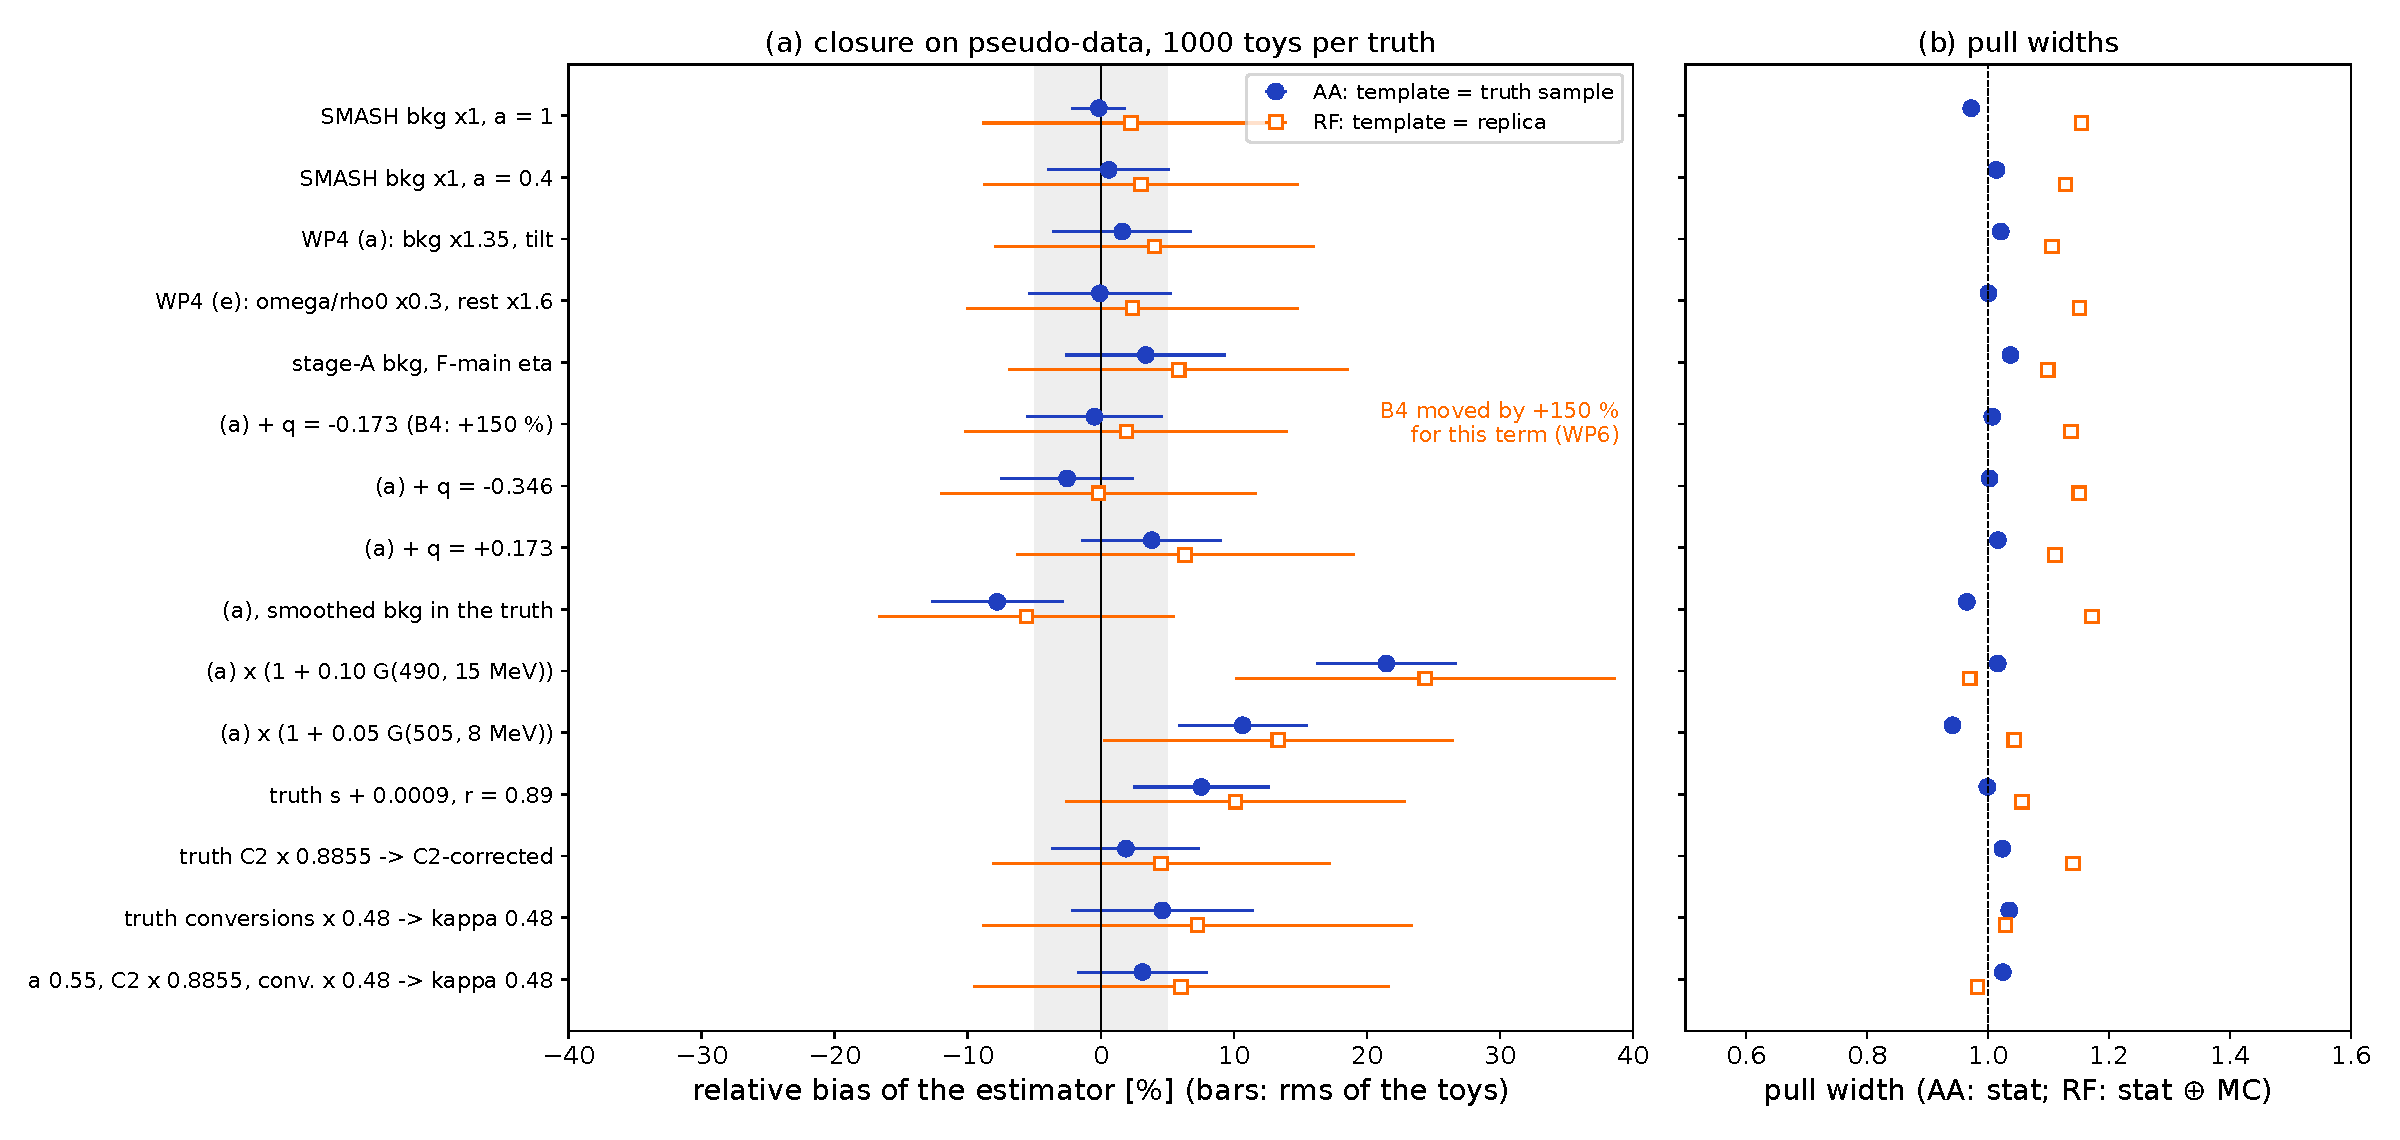
\includegraphics[width=\textwidth]{figs_all/bedge_toys.pdf}
\caption{\textbf{What it shows: the edge estimator recovers the truth within 2\,\% (4\,\% with replica templates); the background term that moves B4 by
$+150$\,\% moves it by 2\,\%; only a background structure as narrow as the edge biases it, and the two other truths outside $\pm5$\,\% are the
template noise and the direction of family E3, both counted.}
Selection: no data; pseudo-data of the edge spectra of S0 (PT3 trigger, event vertex in the target region ($\vz>-160$\,mm), \betanew particle identification (pions within $3\sigma$, leptons within $5\sigma$ and with a RICH ring), energy-loss-corrected momenta of all four tracks, all stored combinations of each event (isBest $\ge0$), both pions in the event-vertex fit) in the \Mpipi slices 0.30--0.34, 0.34--0.37, 0.37--0.39, 0.39--0.40\,\GeVcc and \Mee $<10$, $\ge10$\,\MeVcc, 2.5\,\MeVcc bins: data CB (like-sign counts Poisson-fluctuated, CB rebuilt) + smoothed SMASH non-$\eta$ background $\times\,c\,(1+bx+qx^2)$ + raw SMASH $\eta$ classes (SMASH p+p at 4.5\,GeV (standard, lepton and $\eta$ sets, mode A) at its cross sections $\times$ PDG BR $\times$ the $\eta$-decay weights V3, masses moved to the data scale ($M_4'=0.99615\,M_4$, $\Mpipi'=0.9952\,\Mpipi$)); estimator: the frozen edge fit (edge $\pm45$\,\MeVcc, $\pm35$ in 0.39--0.40) over the simulated step.
(a) Relative bias of the estimator for 15 truths, 1000 pseudo-data sets each. Blue full: templates $=$ the truth sample (AA); orange open: templates
$=$ a bootstrap replica (RF). Bars: rms of the pseudo-data sets; grey band: $\pm5$\,\%. The last three truths use the matching estimator (C2
corrected; $\kappa=0.48$). (b) Pull widths (AA: stat; RF: stat $\oplus$ robust MC).}
\label{fig:bedge-toys}
\end{figure}

\subsection{The C2 decay angle and the converted photons: the readings}
\label{sec:bedge-c2}
\textbf{C2 decay angle (D35).} HGeant decays the virtual photon of $\piz\to\gamma\ee$ isotropically; QED wants $1+\cos^2\theta^*$ (\S\ref{sec:eff}).
WP8 measured the effect on the C2 efficiency with a toy (0.880 / 0.889 / 0.868 for all / E1 / E2) and with the lepton/standard closure (0.891 / 0.869
/ 0.896). A new toy copies the WP8 generator, adds \Mfour and \Mpipi, and applies the frozen edge fit to isotropic and QED-weighted spectra: the
ratio of the summed steps is 0.8826 (all \Mee; E1 0.898, E2 0.863), against 0.8802 for the WP8 quantity over all \Mfour. \textbf{The WP8 factors
therefore hold at the edge within 1\,\%.} Variants: $p_e>0.04$ / $0.10$\,\GeVc give 0.904 / 0.859, a smearing of 6.1\,\MeVcc 0.882; the factor
uncertainty of D35 was $\pm0.024$ (family E8, then 1.4\,\%; with the per-count weights of D38 the model allowance is $\pm0.004$, 0.2\,\%). The E1 value of the edge toy changes from 0.898 to 0.886 between two smearings that leave the slice
ratios unchanged; it is not used (with the edge-toy E1/E2 factors the corrected scale would be 0.4191 instead of 0.4184). With C2 making
53.6\,\% of the simulated step, the constant factor raised $f_\eta(\mathrm{edge})$ by 6.8\,\%, from 0.392 to 0.418. A per-count check of the factor
with the full simulation (\S\ref{sec:c2recon}) showed that the per-slice fit needs 0.860, not 0.881; with these per-count weights (D38, approved)
the correction is $+8.1$\,\%, to 0.423. The visible yield hardly changes (21\,445 $\to$ 21\,353 counts), because the correction acts on the
efficiency, not on what is seen.

\notebox{\textbf{D35 (decision of the lead analysis, approved by the analyst on 15 November 2026).} The bump scale from the edge is quoted \emph{with} the C2
angle correction as the recommended physics value: $f_\eta(\mathrm{edge})=0.418\pm0.022\,(\mathrm{stat})\pm0.035\,(\mathrm{syst})\pm0.047\,(\mathrm{MC})$,
$\sigeta=0.437\pm0.023\pm0.036\pm0.049\,^{+0.042}_{-0.044}\,(\mathrm{norm.})$\,mb. It is quoted \emph{without} the correction for comparison with
the frozen Part~III convention: 0.392 and 0.409\,mb. In that convention WP8 had decided that the angle effect is ``a systematic of known sign,
not a correction'', because a proper correction needs the true \piz frame of every simulated entry. The edge toy shows that the toy and closure factors
apply at the edge itself, and family E8 covers their spread (0.86--0.91). The verifier confirmed the arithmetic and asked for an explicit decision; this
is it. The peak-based \sigeta is not affected ($-0.1$\,\%). Since D38 (approved on 15 November 2026) the constant factor is replaced by
per-count QED weights: $f_\eta(\mathrm{edge})=0.423\pm0.023\pm0.038\pm0.048$ and $\sigeta=0.442$\,mb (with the peak-tail family of D40).}

\textbf{The converted photons.} Part~III leaves open whether SMASH simulates too many conversion pairs (\S\ref{sec:p2}): the peak gives $0.237\pm0.049$
from its conversions and $0.497\pm0.059$ from its direct decays, a conversion scale $\kappa=0.48\pm0.11$. Applied to the bump (C3 $\times0.48$; this
assumes the same scale for the softer \piz photon as for the photon of $\eta\to\pipi\gamma$, in the same material), the edge gives
$0.569\pm0.031\pm0.071\pm0.084$ and $\sigeta=0.594$\,mb (0.513 and 0.536\,mb without the C2 correction); family E9 ($\pm0.11$ on $\kappa$) adds 7.2\,\%.
The bump's own E1/E2 split gives $\kappa=0.47\pm0.24\,(\mathrm{stat})\pm0.46\,(\mathrm{MC})$ and $a_D=0.57\pm0.09\pm0.24$, consistent with the
values from the peak (routes 0.48, side bands per class $0.37\pm0.23$, X17 2D fit 0.51, F-main E1+E2 $0.50\pm0.16$) but limited by the simulation
statistics. \textbf{The bump does not decide between the two readings}; it moves together with the peak: $\sigeta\approx0.43$--0.44\,mb with
$\kappa=1$, 0.52--0.59\,mb with $\kappa=0.48$.

\subsection{The C2 factor at the edges from a per-count weight (D38)}
\label{sec:c2recon}
\inshort{a per-count QED weight shows that both edge fits need a C2 factor of about 0.86, against the effective 0.881 of the constant factor of
D35, which left the bump values 1.2--1.4\,\% low (inside its $\pm0.024$ allowance, but always in the same direction). The analyst approved the
per-count weights on 15 November 2026 (D38): every bump-edge number of this report uses them, until a future simulation corrects the angle in
GEANT itself (not expected). An independent verifier rebuilt the chain with own code and confirms the factors to 0.0004.}

\textbf{What was done, in plain words.} Every simulated C2 entry (1649 in ``pre'', 1514 in S0, standard set) was given its own QED weight
$w=3[1+c^2+\epsilon(1-c^2)]/(4+2\epsilon)$, the ratio of the QED $\gamma^*$ decay angle to the isotropic one of HGeant ($c=\cos\theta^*$,
$\epsilon=4m_e^2/\Mee^2$). The lost photon is not stored, so $w$ was averaged along the circle on which the photon must lie (fixed by the four true
charged momenta, the \piz mass and the $\eta$ mass), with the SMASH $\eta$ density as the weight along it: the mean of $w$ given everything the
analysis sees. Checks: a toy with the true photon reproduces the true mean to 0.0004 in every subset and for every lepton threshold; the 359
full-simulation entries in which the ECAL found the photon give 0.8659 with the exact photon and 0.8671 from the circle; the independent code of the
ECAL study (\S\ref{sec:ecalacc}) agrees entry by entry (rms $2\times10^{-6}$); the density hardly matters (0.0002 between SMASH sets and binnings;
$+0.003$ with no density at all). The reweighted C2 templates went through each estimator's own, unchanged code (it reproduces the nominal
numbers first).

\begin{table}[H]
\centering
\caption{\textbf{What it shows: the edge fits need a C2 factor of 0.860--0.861, about 0.02 below the constant factor of D35; the ECAL-tagged
combinations need 0.876.} Circle average of the QED weight per simulated entry, S0 (mode A, V3), weighted as each estimator weights the entries;
``constant factor (D35)'' is the effective factor of the constant E1/E2 factors, replaced by the per-count weights since D38. Source: \code{c2recon_table.txt} (\fpath{/hdd3/przygoda/HADES/FAT_out/all_report/c2recon/}).}
\label{tab:c2recon}
\small
\resizebox{\textwidth}{!}{%
\begin{tabular}{@{}l c c c c l@{}}
\toprule
estimator or region & all & E1 & E2 & stat & constant factor (D35) \\
\midrule
$u$-edge fit & 0.8607 & 0.8696 & 0.8560 & $\pm0.0071$ & 0.8813 (0.879 / 0.8825) \\
per-slice edge fit & 0.8599 & 0.8682 & 0.8539 & $\pm0.0098$ & 0.8807 (0.879 / 0.882; quoted 0.8855) \\
ECAL-tagged C2 entries & 0.876 & -- & -- & $\pm0.009$ & 0.876 \\
window: all \Mfour & 0.8637 & 0.8651 & 0.8629 & $\pm0.0027$ & \\
window B & 0.8613 & 0.8642 & 0.8597 & $\pm0.0031$ & \\
at the edge ($-15$ to $+5$\,\MeVcc) & 0.8547 & 0.8580 & 0.8530 & $\pm0.0053$ & \\
far below the edge ($u<-60$\,\MeVcc) & 0.8717 & 0.8554 & 0.8822 & $\pm0.0058$ & \\
\bottomrule
\end{tabular}}
\end{table}

\textbf{Why the earlier numbers differ.} The factor depends mainly on the momentum of the softer lepton: 0.91 at 60--100\,\MeVc, 0.87 at
100--150\,\MeVc, 0.80--0.82 above 200\,\MeVc. In the toys with a sharp 60\,\MeVc cut (WP8 toy 0.880, edge toy 0.883, verifier toys
0.875--0.880) 34\,\% of the accepted decays have a softer lepton below 80\,\MeVc, in the full simulation only 5\,\%; with a 100\,\MeVc cut the toy
gives 0.862. The closure 0.891 comes from prompt \piz Dalitz pairs with another selection, where PLUTO and HGeant also differ in more than the
angle (its E1/E2 pattern is the reverse of every C2 estimate). E2 carries 66\,\% ($u$) and 57\,\% (per slice) of the C2 step and has the lower
factor; the applied E2 factor (0.882, the mean of toy 0.868 and closure 0.896) causes 0.016--0.017 of the 0.021 gap. The ECAL study's 0.855 at
the edge is a window mean; the step fits weight the entries differently (80\,\% of $h$ comes from just below the edge, entries leaking above it count
negatively) and need 0.860--0.861. Its comparison ``0.855 against 0.8855, $+1.8$\,\%'' is therefore not the right one; 0.860 against the effective
0.881 gives $+1.2$\,\% per slice (0.418 $\to$ 0.423) and $+1.4$\,\% in $u$.

\textbf{The values used (D38) and what they changed.} $u$-edge $0.861\pm0.007\pm0.004$ (simulation statistics, model),
per-slice edge $0.860\pm0.010\pm0.004$, ECAL tag $0.876\pm0.009$ (unchanged: it was already applied per count). With the per-count weights and the
peak-tail family of D40: $f_\eta(u\text{-edge})=0.426\pm0.020\pm0.034\pm0.030$ (syst 8.0\,\%; 7.2\,\% without the peak tail), \sigeta from the bump
$0.444\pm0.021\pm0.035\pm0.031\,^{+0.043}_{-0.044}$\,mb (0.573\,mb with the conversions $\times0.48$); per slice $0.423$ and 0.442\,mb; DR$_u$ 0.97;
visible yields $+0.1$\,\% (B) and $+0.3$\,\% (all \Mfour); $\kappa$ from the \Mee split 0.83 ($u$) and 0.47 (per slice); ECAL best reading
data/expected $0.84\pm0.15$. The allowance (U10, E8) shrank from $\pm0.024$ to $\pm0.004$ (about $\pm0.3$\,\% on $f$), and the MC replicas carry
the factor's error automatically. The C2 correction as a whole is $+9.2$\,\% ($u$) and $+8.1$\,\% (per slice) instead of $+7.7$ and $+6.8$\,\%, and
the simulated C2 efficiency of the bump counts is about 16\,\% too high (12--14\,\% in the toys and the closure). Unchanged: \sigeta from the peak
(0.429\,mb), the ECAL reading ``as is'' (1.16) and every uncorrected reading.

\textbf{Independent verification (vc2recon).} A verifier rebuilt the whole chain with own code: an own dump of the 1649 C2 entries with their true
momenta, an own solution of the photon circle (azimuth measure checked against a flat azimuth in the \ee rest frame to $6\times10^{-6}$), an own
SMASH $\eta$ density from 40 further SMASH files (94\,863 $\eta$), an own kinematic photon match and own reweighted templates passed through the
frozen fit codes (the nominal $u$ fit reproduced to every digit). Result: $u$-edge $0.8606\pm0.0070$, per slice $0.8596\pm0.0097$, ECAL-tagged
$0.8764\pm0.0091$, all within 0.0004 of c2recon, well inside the $\pm0.004$ allowance; $f_\eta(u\text{-edge})$ $0.42004\to0.42577$ ($+1.36$\,\%),
per slice $0.41841\to0.42354$ ($+1.23$\,\%). Physics checks: $\theta^*$ equals the textbook two-step angle to $10^{-10}$ (the lab direction of the
pair as axis would give 0.840 instead of 0.869); the HGeant source (\code{gdalet.F}) samples $\cos\theta^*$ uniformly; the electron-mass term
matters (without it 0.8505 / 0.8477); HGeant already includes a $\rho$-pole form factor, and the PDG slope changes the template by at most 0.0004.
Closure toys of $2\times8\times10^6$ decays give true minus circle $+0.0001\pm0.0001$; a soft-lepton efficiency $\pm20$\,\% moves the factors by
$\mp0.0022$, a flat density (the extreme bound) by $+0.0027$ ($u$) and $+0.0038$ (per slice). Two choices of c2recon are confirmed: the circle
mean in the edge templates (the exact weight wherever a photon was found would bias the $u$ factor by $+0.0012$) and exact weights for the ECAL
tag, whose entries are selected by the found photon. Open: the per-slice E2 factor is 0.0006 lower than c2recon's (0.15 of the allowance; cause
not found). \textbf{Verdict: confirmed.}

\notebox{\textbf{D38 (lead analysis, approved by the analyst on 15 November 2026).} The constant WP8 class factors of the C2 $\gamma^*$ angle
(0.879 / 0.882 per slice, 0.879 / 0.8825 in $u$) are replaced by the per-count circle-mean QED weight (\code{c2recon_weights.txt}): effective 0.861
($u$) and 0.860 (per slice), allowance $\pm0.004$; to be applied until a future simulation corrects the angle in GEANT itself (not expected).
$f$ and \sigeta from the bump rise by 1.4\,\% ($u$: 0.426, 0.444\,mb) and 1.2\,\% (per slice: 0.423, 0.442\,mb), far inside their 12--15\,\%
errors; every bump-edge number of this report uses them. Part~I keeps 0.891 as the closure for prompt \piz pairs. Package c2recon
(\code{plots/all_report/c2recon_*}), verification vc2recon (\code{plots/all_report/vc2recon_*}); note \code{notes_all/c2recon_results.md}.}

\subsection{Comparison with the peak, B4, F-main and the ECAL tag}
\label{sec:bedge-cmp}

\begin{table}[H]
\centering
\caption{\textbf{What it shows: \sigeta from the bump edge lies with the routes of the peak; all are a factor 2--2.5 below SMASH.} PDG 2026;
$\Csec(1-\feta)=1.0104\times0.97$ for the bump, 0.981 for the peak; errors stat $\pm$ syst $\pm$ MC $\pm$ norm.\ where given. The one-sided items
(live time, sorter, \code{cor_ok}, vertex, production model) are not included, as for the peak.}
\label{tab:bedge-sigma}
\footnotesize
\begin{tabularx}{\textwidth}{@{}>{\raggedright\arraybackslash}p{6.1cm} >{\raggedright\arraybackslash}p{5.9cm} L@{}}
\toprule
route & \sigeta [mb] & status \\
\midrule
bump edge, SMASH as is & $0.409\pm0.022\pm0.036\pm0.044\,^{+0.039}_{-0.041}$ & frozen convention \\
\textbf{bump edge, C2 angle corrected} & $\mathbf{0.442\pm0.024\pm0.040\pm0.050\,^{+0.042}_{-0.044}}$ & per slice (D35, D38), PRELIMINARY; cross-check of $u$ (D37) \\
$u$-edge, C2 angle corrected (\S\ref{sec:edgeu}) & $0.444\pm0.021\pm0.035\pm0.031\,^{+0.043}_{-0.044}$ & the bump measurement (D37), PRELIMINARY \\
bump edge, C2 corrected, conversions $\times0.48$ & $0.594\pm0.032\pm0.074\pm0.087\,^{+0.057}_{-0.059}$ & alternative \\
bump edge, uncorrected, conversions $\times0.48$ & $0.536\pm0.029\pm0.063\pm0.074\,^{+0.051}_{-0.053}$ & alternative \\
bump edge, $\kappa$ free (E1/E2 split) & $0.599\pm0.092\,(\mathrm{stat})\pm0.245\,(\mathrm{MC})$ & not a measurement \\
\midrule
peak side bands (adopted) & $0.429\pm0.036\pm0.157\pm0.025\,^{+0.041}_{-0.043}$ & PRELIMINARY \\
peak, direct-decay route / conversion route & $0.522\pm0.062$ / $0.249\pm0.051$ (stat) & alternatives \\
ECAL tag & 0.474 & verification only \\
F-main & 0.399 & cross-check \\
SMASH & 1.069 & model \\
HADES at 3.5\,GeV, inclusive (lower energy) & $1.14\pm0.20$ / $0.93\pm0.14$ & context only \\
\bottomrule
\end{tabularx}
\end{table}

\textbf{Double ratio.} $\mathrm{DR}_{\mathrm{edge}}=\aP/f_\eta(\mathrm{edge})$ (PDG 2026 both) $=0.970\pm0.098\,(\mathrm{stat})\pm0.174\,(\mathrm{syst})
\pm0.124\,(\mathrm{MC})$ with the C2 correction (per-count weights), a total of 24\,\% without the composition term of the peak (with it about $\pm0.37$, as
DR$_u$ of \S\ref{sec:edgeu-cmp}), and $1.049\pm0.106\pm0.189\pm0.130$ without it; B4 gave 1.373 (not determined) and
F-main 1.148. The systematic error of \aP enters without the composition term of the peak (16.0\,\%, not the 36.6\,\% of \sigeta), because the composition largely
cancels between peak and bump. With the conversions scaled by 0.48 on both sides (direct-decay route over the $\kappa$-scaled edge) the double
ratio is $0.497/0.567=0.88$. \textbf{Peak and bump therefore see the same data/SMASH ratio within the 25\,\% uncertainty of the double ratio.} The
agreement of the cross sections, 0.442 against 0.429\,mb, is a weak test, because the peak value carries 38\,\%; with $\kappa=0.48$ the bump gives
$0.594\pm0.13$\,mb against $0.522\pm0.062$\,mb from the direct decays of the peak.

\textbf{ECAL tag} (verification only; the ECAL recalibration is pending): $f_\eta(\mathrm{tag})=0.454\pm0.043$, \sigeta 0.474\,mb, between the
readings with $\kappa=1$ and $\kappa=0.48$. The full reconstruction with the ECAL photon is a feasibility study: data/expected $1.16\pm0.21$ with
the simulated photon-energy scale, $0.84\pm0.15$ with a data-like one (\S\ref{sec:ecalacc}).

\textbf{Items not in the totals} (as for the peak; they act on every absolute $\eta$ scale): live time $+7.1$ to $+7.3$\,\%, sorter $+1.3$ to
$+2.8$\,\%, \code{cor_ok} $+2.2$\,\%, the vertex factor of the bump $C_{\mathrm{vtx}}=0.999\pm0.022$, the production model ($p_T$ $+21$\,\%, $y$
$-8$\,\%), $\feta=12$\,\% ($-9$\,\%). Specific to the edge: $r_{\mathrm{res}}=0.89$, favoured by the measured peak width, gives $-5.5$\,\% (0.370;
counted symmetrically in family E3).

\begin{figure}[!htbp]
\centering
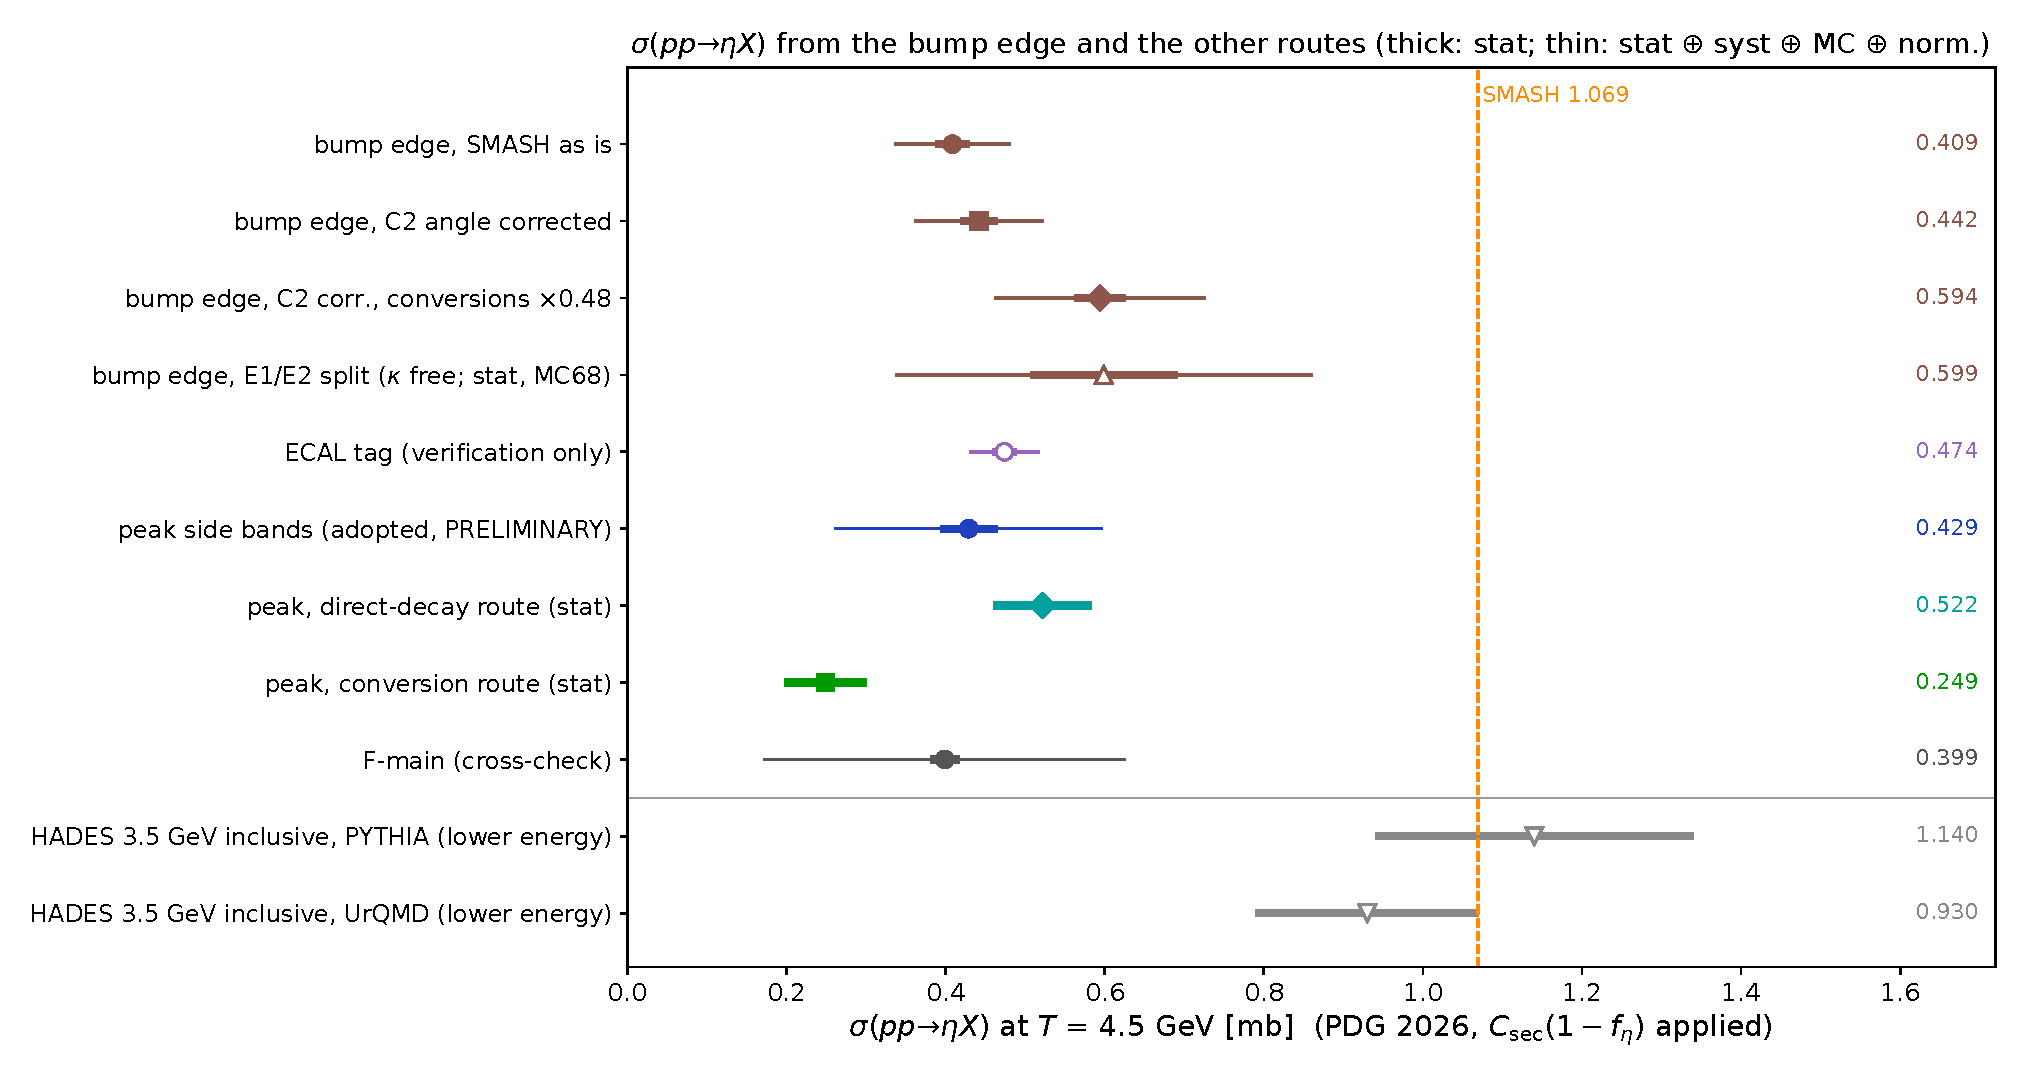
\includegraphics[width=0.92\textwidth]{figs_all/bedge_sigma_v3.pdf}
\caption{\textbf{What it shows: \sigeta from the bump edge (0.41--0.44\,mb, or 0.59\,mb with the conversions $\times0.48$) agrees with the routes of
the peak; all lie a factor 2--2.5 below SMASH and below the published HADES values at 3.5\,GeV.}
Selection: data, S0 (PT3 trigger, event vertex in the target region ($\vz>-160$\,mm), \betanew particle identification (pions within $3\sigma$, leptons within $5\sigma$ and with a RICH ring), energy-loss-corrected momenta of all four tracks, all stored combinations of each event (isBest $\ge0$), both pions in the event-vertex fit), each value with its own windows: bump edge in the \Mpipi slices 0.30--0.34, 0.34--0.37, 0.37--0.39, 0.39--0.40\,\GeVcc (all \Mee), carried over the bump window 0.4550--0.5225\,\GeVcc with the simulated bump shape; peak side bands (peak window 0.53364--0.55416\,\GeVcc, side bands 0.5250--0.5336 and 0.5542--0.5628\,\GeVcc, all \Mee); routes (side bands per \Mee class, X17 fit in \Mfour 0.5225--0.6100\,\GeVcc $\times$ \Mee 2--62\,\MeVcc); ECAL tag; F-main (\Mee$\ge10$\,\MeVcc, \Mfour 0.400--0.700\,\GeVcc); SMASH as SMASH p+p at 4.5\,GeV (standard, lepton and $\eta$ sets, mode A) at its cross sections $\times$ PDG BR $\times$ the $\eta$-decay weights V3, masses moved to the data scale ($M_4'=0.99615\,M_4$, $\Mpipi'=0.9952\,\Mpipi$), same cuts.
PDG 2026; $\Csec(1-\feta)=1.0104\times0.97$ (bump), 0.981 (peak). Brown: the bump-edge readings (open triangle: $\kappa$ free, stat and robust
MC only); violet open circle: ECAL tag (verification only); blue: peak side bands (adopted, PRELIMINARY); cyan and green: the direct-decay and
conversion routes of the peak (stat only); grey: F-main (cross-check); grey open triangles: HADES inclusive values at 3.5\,GeV (lower energy;
context only); dashed orange line: SMASH, 1.069\,mb. Thick bars: stat; thin: stat $\oplus$ syst $\oplus$ MC $\oplus$ norm. Right: central values.
The one-sided items of Part~III (vertex, live time, sorter, \code{cor_ok}, production model) are not included.}
\label{fig:bedge-sigma}
\end{figure}

\subsection{Why the edge works where B4 failed}
\label{sec:bedge-why}
B4 measures the \emph{area} of the bump: it needs the background under the whole bump window, and that background can only be carried
40--120\,\MeVcc down from above the peak (\S\ref{sec:b4}); any curvature of the background changes the area, by $+150$\,\% for the quadratic term
that the data allow. The edge measures the \emph{height of a step} that only the $\eta\to3\pi$ kinematics can make: across the 10--20\,\MeVcc around
the edge a smooth background is absorbed by the polynomial, so the same quadratic term moves the edge by only $-2$\,\%. The price is that the
yield in the window follows from the step through the simulated shape of the bump ($f_\eta\times$ SMASH's C2+C3 in B); this shape is the
$\eta\to3\pi$ kinematics with the measured (KLOE-2) Dalitz plot, and the three readings, which compose the simulated bump differently, give
21\,353--21\,744 counts. What B4 lacks is therefore not data but a measured background; the edge does not need one.

\subsection{Caveats}
\label{sec:bedge-cav}
\begin{enumerate}\setlength{\itemsep}{1pt}
\item \textbf{Simulation-limited.} The MC error (11\,\%) is twice the statistical one (5.4\,\%). Taking the simulated step from the bump classes
      alone (no smoothing model) would give about 6.6\,\% (verifier vedgeu); the $u$-edge does this (MC 7.0\,\%, \S\ref{sec:edgeu}).
\item \textbf{Background structures as narrow as the edge} would bias it ($+21$\,\% for a 10\,\% bump of 15\,\MeVcc width, $+11$\,\% for 5\,\% and
      8\,\MeVcc). None is present in SMASH, and the data control slice without a bump shows $h=15\pm15$ counts (bump slices: 135--389). The method relies on this.
\item \textbf{$\kappa=0.48$} comes from the peak routes, mostly from the X17 2D fit (82\,\% of the weight); using it for the bump assumes the same
      conversion scale for the \piz photon as for the photon of $\eta\to\pipi\gamma$.
\item \textbf{The C2 correction} first rested on toys with a simple acceptance and on the WP8 closure, whose class pattern differs (toy: E2
      more affected; closure: E1); the edge toy confirmed the all-\Mee factor within 1\,\%. Since D38 (approved) the per-count average of the full
      simulation is used (0.860 for this fit, \S\ref{sec:c2recon}): $f=0.423$, 1.2\,\% above the constant factor of D35; family E8 is its model
      allowance, $\pm0.004$.
\item \textbf{$r_{\mathrm{res}}$} is the largest counted item (family E3). The data peak width ($5.44\pm0.60$\,\MeVcc against 6.09 simulated) favours
      $r_{\mathrm{res}}=0.89$, which gives 0.370 ($-5.5$\,\%); counted symmetrically, as in WP7.
\item \textbf{Family E7} rests on the smoothing; its sign is not known (exp(pol2)--exp(pol5) give $-0.010$ to $+0.030$ for a stage-A-like background).
\item \textbf{The \Mee classes E1 and E2 differ} (0.367 against 0.431; C2 corrected 0.386 against 0.487), by 0.5--0.7$\sigma$. The difference may be $\kappa$, the E1
      background ($\kEone=7.6$ in Part~III) or MC noise; the edge cannot separate them.
\item \textbf{The absolute \sigeta} inherits the PRELIMINARY status of Part~III: the one-sided items are not included. $\mathrm{DR}_{\mathrm{edge}}$
      does not depend on them.
\item \textbf{Folds and periods} are marginal ($p\approx0.05$ and 0.07; IIB high, III low), below the WP7 threshold.
\item The data bootstrap treats unlike-sign and like-sign event groups as independent, as WP0's CB replicas; the $N$--CB correlation is
      neglected, as in WP4/WP6.
\item \textbf{Blinding}: only the \Mee classes split at 10\,\MeVcc were used; no X17 cell and no 2\,\MeVcc \Mee shape.
\end{enumerate}

\textbf{Verification} (vbedge, own code: own pass over the entries and own bootstrap, own edge fitter). Every decisive number is reproduced exactly: $E_{\mathrm{data}}$,
$E_{\mathrm{sim}}$, $f_\eta(\mathrm{edge})=0.39162$, the C2-corrected 0.41841, the $\kappa=0.48$ reading 0.56021 (both with the constant C2 factor of D35; with the
per-count weights of D38 0.42345 and 0.56927), \Ybump(B) $=21\,445$ counts, \sigeta $=0.409$ / 0.437 / 0.585\,mb (D35 factor), the four tested variants, the periods and the control slices. Stat 0.0201 (own seeds) against 0.0210, MC
0.0376 against 0.0425. Corrected in the text above, as the verifier asked: the rejection of the Dalitz-plot variants (now based on KLOE-2 and WP7
R1), the sign of family E7 (unknown; symmetric envelope), the template-statistics bias ($+0.8$\,\%, not $+2.4$\,\%), the precision of
$\mathrm{DR}_{\mathrm{edge}}$ (24\,\%, without the composition term) and the fold test (marginal); the C2 convention is decided explicitly (D35).
\textbf{Verdict: numbers confirmed.}

%======================================================================
\section{The \texorpdfstring{$\eta$}{eta} bump in the distance to its kinematic edge, \texorpdfstring{$u$}{u}}
\label{sec:edgeu}
%======================================================================
\inshort{every bump combination has its own kinematic edge $E(\Mpipi,\Mee)$; in the distance to it, $u=\Mfour-E$, all edges fall on $u=0$ and
one fit finds a step of 21$\sigma$. The bump holds $f_\eta(u\text{-edge})=0.426\pm0.020\,(\mathrm{stat})\pm0.034\,(\mathrm{syst})\pm0.030\,(\mathrm{MC})$
of the SMASH $\eta$ (C2 decay angle corrected with per-count QED weights, D35, D38; peak-tail family included, D40; 0.390 uncorrected), the visible
yield in window B is $21\,468\pm1003\pm1708\pm1347$ counts and the bump alone gives $\sigeta=0.444$\,mb. The per-slice edge of \S\ref{sec:bedge}
agrees (0.423, 0.442\,mb); like for like, $u$ is somewhat more precise (11.6 against about 12.4\,\%), but not less model dependent. A step of the
$e^-e^-$ like-sign counts at $u=0$ (4.7$\sigma$) is explained: lepton pairs from the two \piz photons, which the CB removes as designed (D39,
independently verified). The low-mass tail of the SMASH peak term, the leptons' radiation in the material, reaches the edge and moves $f$ by
$+6.8$\,\% per unit of its size; the data cannot fix that size, and a term of $\pm3.4$\,\% is counted (D40). $u$ is the bump measurement (D37);
D37--D40 were approved by the analyst on 15 November 2026.}

\begin{table}[H]
\centering
\caption{\textbf{What it shows: the bump measured in $u$ in its three readings and what follows from them.} S0, isBest $\ge0$,
$0.30\le\Mpipi<0.40$\,\GeVcc, $L=6079.2\,\nbinv$; yields are raw counts $\times64/63$ in window B (0.4550--0.5225\,\GeVcc), all \Mee. Errors: stat
(200 bootstrap copies of the data), syst (families U1--U11, Table~\ref{tab:edgeu-syst}), MC (rms of 100 simulation replicas), and for \sigeta
the normalisation ($L$ 6.9\,\%, period 5\,\%, BR 3.17\,\%, $\Csec(1-\feta)$ $^{+3.1}_{-4.1}$\,\%). \sigeta $=f/1.00436$ (PDG 2026) $\times1.0694$\,mb
$\times1.0104\times0.97$. $Y/L$ carries in addition $L\oplus$ period (8.5\,\%). DR$_u$ includes the composition term of the peak (35.5\,\%
systematic of \aP; verifier vedgeu). Source: \code{tables_all/edgeu_results_v3.txt} (\code{edgeu_combine_v3.py}: per-count C2 weights, D38;
peak-tail family in U8, D40).}
\label{tab:edgeu-res}
\footnotesize
\resizebox{\textwidth}{!}{\tabin{edgeu_results_v3_cnt.tex}}
\end{table}

\subsection{The procedure in plain words}
\label{sec:edgeu-proc}
\begin{enumerate}\setlength{\itemsep}{1pt}
\item \textbf{Why $u$.} In the bump an $\eta$ decays into \pipi\piz, the \piz gives an \ee pair and one photon is not detected. The four detected
      particles then always have a mass below a limit, reached when the lost photon is as soft as possible. That limit depends on \Mpipi (it fixes
      how fast the \piz moves in the $\eta$ frame) and on \Mee (it fixes how much energy the photon gets in the \piz frame; a heavier pair leaves
      less for the photon). So every bump combination carries its own edge, and $u=\Mfour-E(\Mpipi,\Mee)\le0$ for every bump combination, whatever its \Mpipi and
      \Mee. The per-slice method (\S\ref{sec:bedge}) cut \Mpipi into four slices with an edge that moves inside each slice by 4.7--7.1\,\MeVcc and
      ignores \Mee; in $u$ there is one sharp step at $u=0$.
\item \textbf{The edge function.} The frozen edge of \code{defs.h} (Eq.~\ref{eq:edge}) already contains the \Mee term. On the data scale
      $E(m,q)=0.99274\,M_4^{\max}(m/0.9970,q)$, with $M_4^{\max}(m,q)^2=m_\eta^2-m_\eta(E_{\piz}-p_{\piz})(1-q^2/m_{\piz}^2)$; the simulated entries
      are first transferred to the data scale (D8) and then get the same $E$. \Mee is not scaled.
\item \textbf{The fit.} One fit in $u$ over $-45\le u<+45$\,\MeVcc (36 bins of 2.5\,\MeVcc, a bin edge at $u=0$): a smooth part (pol2) plus a step
      of height $h$ at $u=0$, smeared with the simulated template width (6.70\,\MeVcc). The CB is $2\sqrt{N_{++}N_{--}}$ in 10\,\MeVcc cells of $u$ per
      \Mpipi slice (the rule of the report applied to $u$). The $\eta$ peak, at $u=+20$ to $+55$\,\MeVcc, is a fixed term $\aP\times K(u)$ ($K$ =
      SMASH C4+C5, $\aP=0.418$).
\item \textbf{The ratio.} The same linear estimator applied to the simulated bump classes alone (C2+C3, C2 with its per-count QED weight, D38;
      effective 0.861) gives $h_{\mathrm{sim}}$; $f_\eta(u\text{-edge})=h_{\mathrm{data}}/h_{\mathrm{sim}}$.
\item \textbf{Errors.} 200 bootstrap copies of the data (stat), 100 simulation replicas (MC), 70 variants in eleven families U1--U11 with the WP7
      rules (syst); 21 pseudo-data truths with 1000 toys each.
\item \textbf{Checks.} Each \Mpipi slice, each \Mee class, periods, folds, isBest $=1$, ``pre'', and null tests: like-sign counts of the data, simulated
      non-bump classes, a data region without bump.
\end{enumerate}

\subsection{The kinematics and the simulated truth}
\label{sec:edgeu-kin}
In the simulated truth not one bump entry lies above its edge: the largest excess of $m_4^{\mathrm{true}}-M_4^{\max}(\Mpipi^{\mathrm{true}},
\Mee^{\mathrm{true}})$ is $-0.48$\,\MeVcc for C2 (1649 simulated entries) and $-0.51$\,\MeVcc for C3 (1187). Without the \Mee term ($E(m,0)$), 3.8\,\% of C2
lie above the edge by more than 1\,\MeVcc and 1.8\,\% by more than 5\,\MeVcc; C3 (median true \Mee 2\,\MeVcc) is not affected. At $m=0.30$\,\GeVcc
the edge moves from 0.5186 ($q=0$) to 0.5221 ($q=50$\,\MeVcc) and 0.5326\,\GeVcc ($q=100$\,\MeVcc). Reconstructed, 0.85\,\% of C2 and 1.04\,\% of C3
lie above $u=+10$\,\MeVcc: the resolution tail. The template width at the edge is 6.70\,\MeVcc (Gaussian fit on $\pm40$\,\MeVcc; 5.8--7.1\,\MeVcc
with other ways of fitting the core, which change $f$ by less than 0.3\,\%); almost all of it is the error of \Mfour, the error of the edge from
\Mpipi and \Mee is only 1.2\,\MeVcc. Near the edge the \ee pair carries almost the whole \piz momentum, so the \Mfour resolution there is close to
that of the $\eta$ peak (Fig.~\ref{fig:edgeu-kin}).

\begin{figure}[!htbp]
\centering
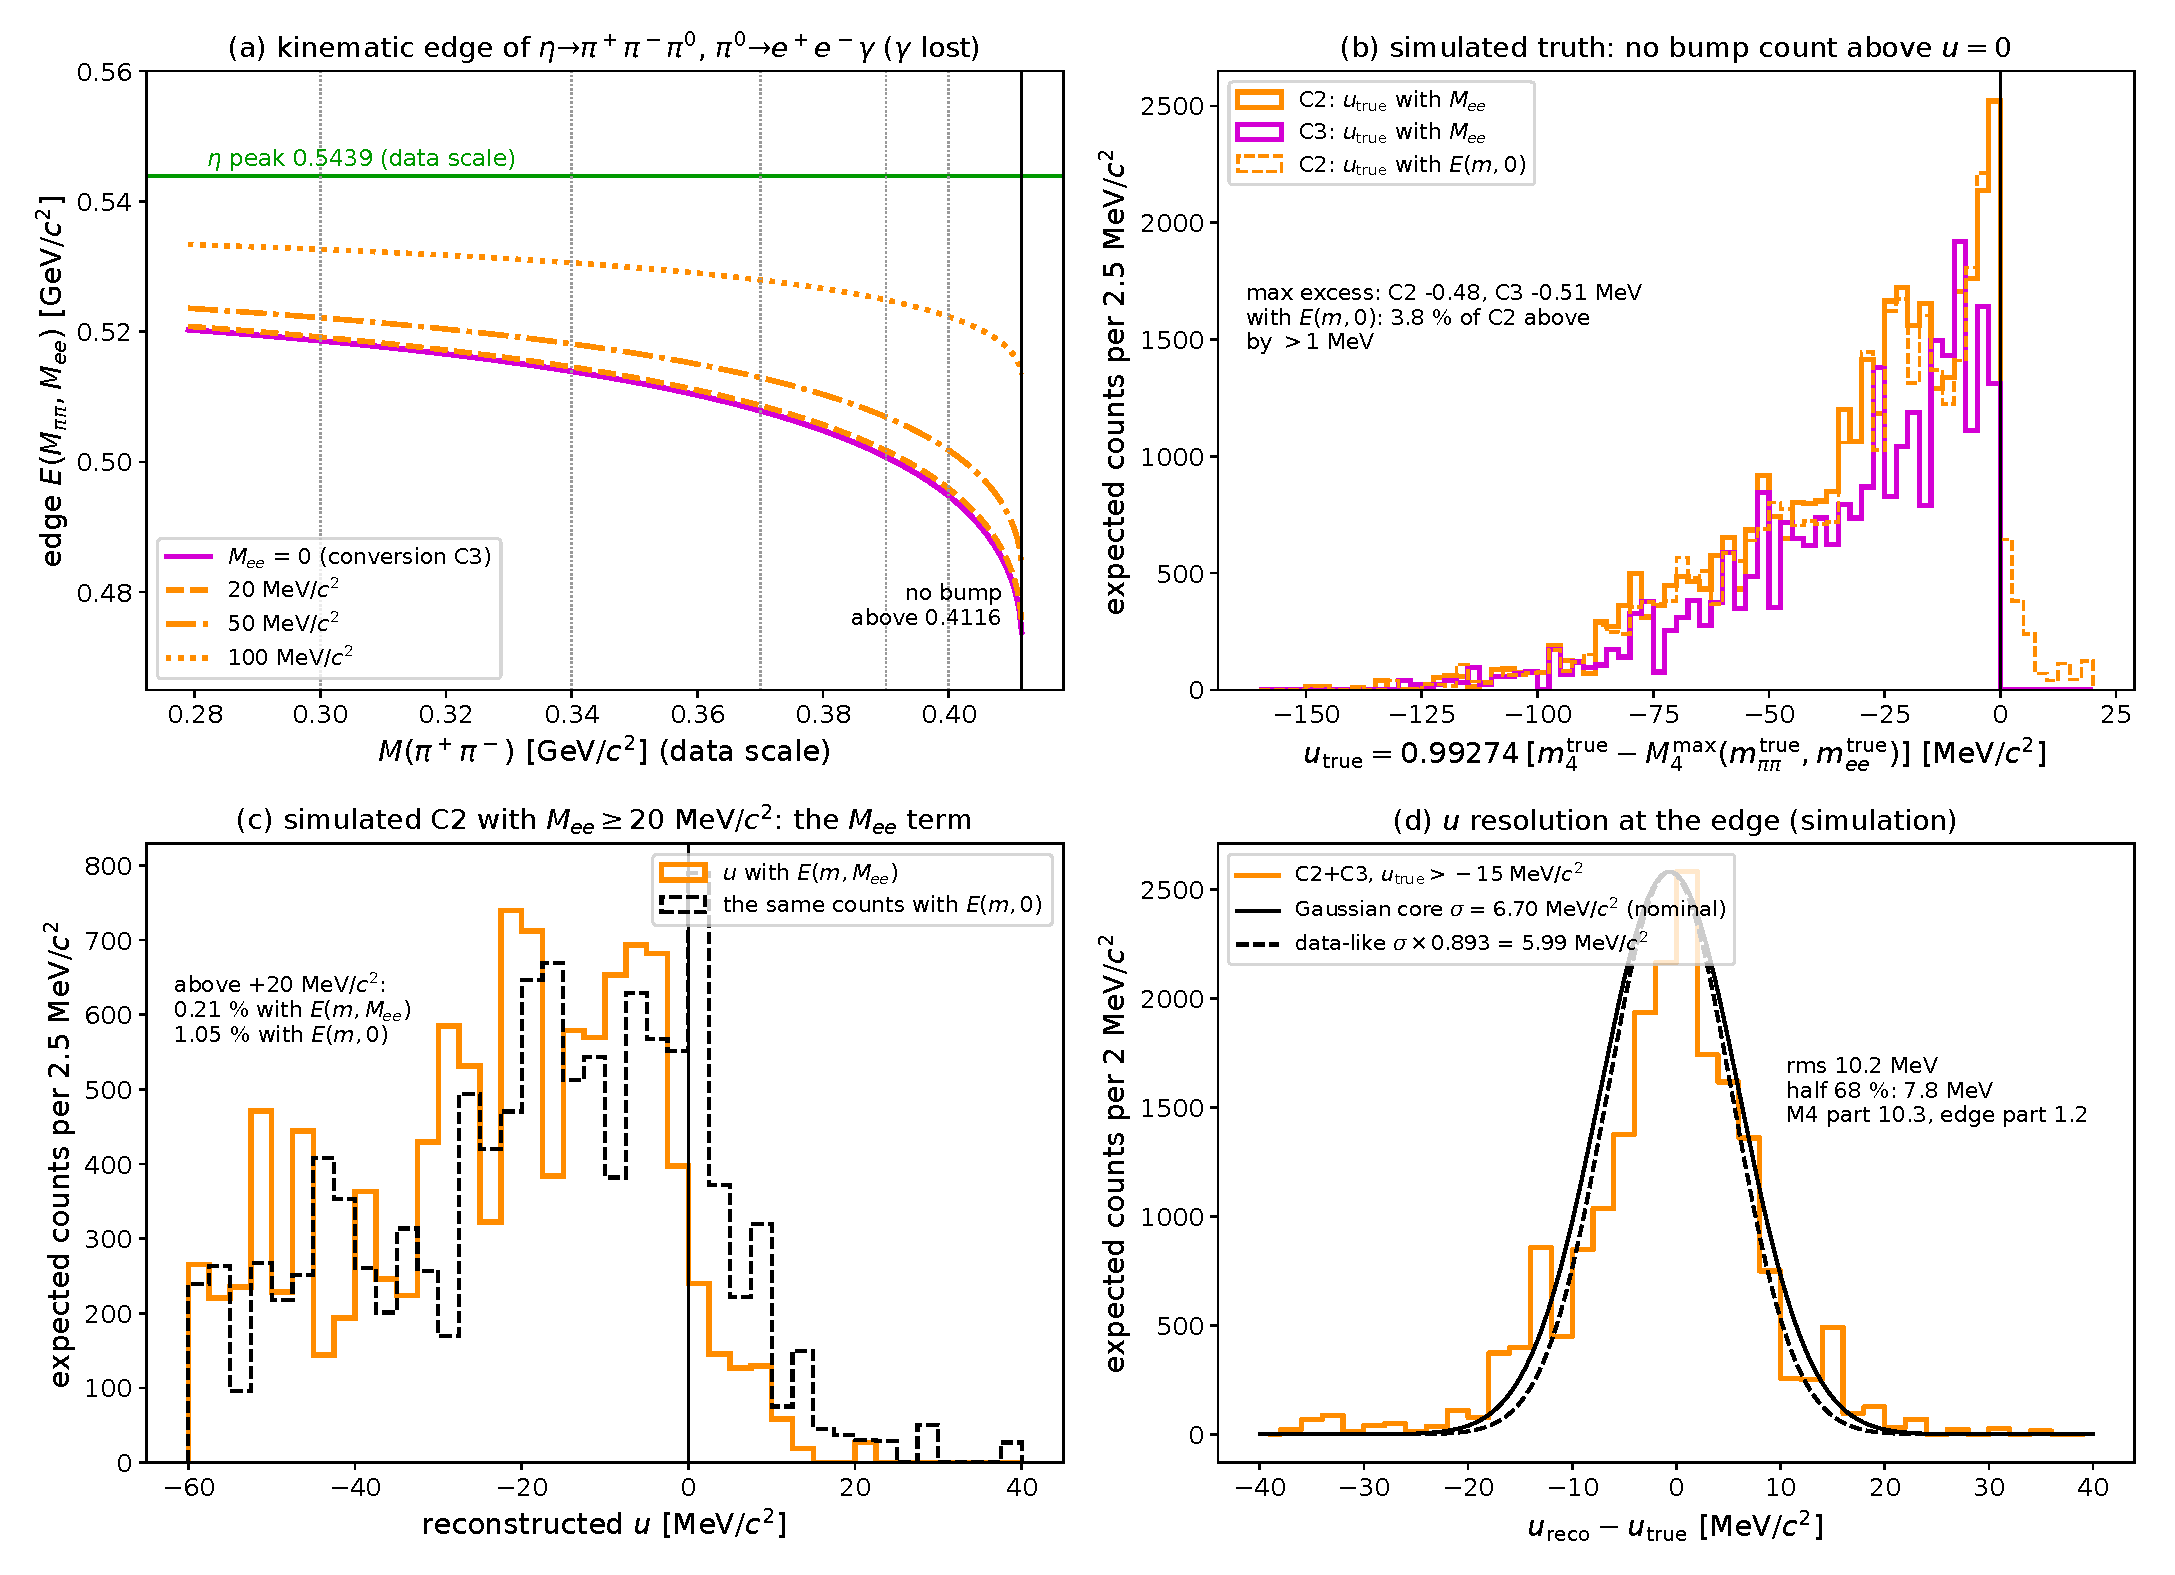
\includegraphics[width=0.86\textwidth]{figs_all/edgeu_kinematics_cnt.pdf}
\caption{\textbf{What it shows: the edge of the bump depends on \Mpipi and \Mee; once both are taken into account no simulated bump count lies above
it, and the reconstructed $u$ is smeared by about 6.7\,\MeVcc.}
Selection: simulation only: SMASH p+p at 4.5\,GeV (standard, lepton and $\eta$ sets, mode A) at its cross sections $\times$ PDG BR $\times$ the $\eta$-decay weights V3, masses moved to the data scale ($M_4'=0.99615\,M_4$, $\Mpipi'=0.9952\,\Mpipi$), S0 cuts (PT3 trigger, event vertex in the target region ($\vz>-160$\,mm), \betanew particle identification (pions within $3\sigma$, leptons within $5\sigma$ and with a RICH ring), energy-loss-corrected momenta of all four tracks, all stored combinations of each event (isBest $\ge0$), both pions in the event-vertex fit); (a) the edge function alone; (b)--(d) $0.30\le\Mpipi'<0.40$\,\GeVcc: (b) C2 and C3 at their true masses, (c) C2 with \Mee$\ge20$\,\MeVcc, (d) C2+C3 with $u_{\mathrm{true}}>-15$\,\MeVcc.
(a) The edge $E(\Mpipi,\Mee)$ on the data scale for \Mee $=0$, 20, 50, 100\,\MeVcc; green: the $\eta$ peak 0.5439\,\GeVcc; dotted: the slice
boundaries of the per-slice edge; no bump above \Mpipi $=0.4116$\,\GeVcc. (b) Simulated truth $u_{\mathrm{true}}=0.99274\,[m_4^{\mathrm{true}}-
M_4^{\max}(\Mpipi^{\mathrm{true}},\Mee^{\mathrm{true}})]$ for C2 (orange) and C3 (magenta); dashed: C2 with the edge at \Mee $=0$ (counts above
$u=0$). (c) Reconstructed $u$ of simulated C2 with \Mee$\ge20$\,\MeVcc, with the \Mee term (orange) and without it (dashed). (d)
$u_{\mathrm{reco}}-u_{\mathrm{true}}$ near the edge (C2+C3, $u_{\mathrm{true}}>-15$\,\MeVcc) with the template width (6.70\,\MeVcc, Gaussian fit on
$\pm40$\,\MeVcc; 5.8--7.1\,\MeVcc depending on the fit method) and the data-like width $\times0.893$. SMASH mode A, $w\times$V3, S0,
$M_4'=0.99615\,M_4$, $\Mpipi'=0.9952\,\Mpipi$, expected raw counts at $L=6079.2\,\nbinv$.}
\label{fig:edgeu-kin}
\end{figure}

\subsection{Spectra and null tests}
\label{sec:edgeu-spec}
In the data ($0.30\le\Mpipi<0.40$\,\GeVcc, S0) $N-\mathrm{CB}$ rises up to $u=-5$\,\MeVcc (3870 counts per 2.5\,\MeVcc), drops to 3420 at $+6$\,\MeVcc
and rises again into the peak; the CB is about 200--215 counts per bin in the fit range, 6\,\% of $N$; ``pre'' has 38\,\% more counts and the same shape.
In SMASH the bump classes end at $u=0$, the peak lies at $u=+15$ to $+60$\,\MeVcc, and the non-$\eta$ backgrounds and \Geta are smooth within their
template noise, which is large ($N_{\mathrm{eff}}$ per 5\,\MeVcc bin 64--330 for $G_D$, 18--105 for $G_C$, 14--52 for \Geta; Fig.~\ref{fig:edgeu-spec}).
The step height of the nominal estimator in samples that should have no step:
\begin{center}\small
\begin{tabularx}{\textwidth}{@{}>{\raggedright\arraybackslash}p{5.9cm} L >{\raggedright\arraybackslash}p{3.3cm}@{}}
\toprule
sample & step $h$ [counts per 2.5\,\MeVcc] & verdict \\
\midrule
data, like-sign $e^+e^+$ ($N_{++}$) & $2.1\pm6.5$; at \Mee$\ge90$\,\MeVcc $7.3\pm4.3$ & no step overall; at large \Mee the expected small step (\S\ref{sec:edgeu-ls}) \\
data, like-sign $e^-e^-$ ($N_{--}$) & $73.5\pm15.7$ (\Mee$<10$: $-5.4\pm4.6$; \Mee$\ge10$: $78.7\pm15.0$); \Mee$<50$: $3.6\pm8.9$; 50--90: $13.0\pm9.1$; $\ge90$: $57.0\pm9.1$ & step, 4.7$\sigma$: pairs from the two \piz photons (\S\ref{sec:edgeu-ls}) \\
$N_{++}+N_{--}$ & $75.7\pm17.0$ & step \\
the CB as subtracted, $2\sqrt{N_{++}N_{--}}$ & 39.2 (3.0\,\% of $h_{\mathrm{data}}$) & counted in U5 \\
SMASH $G_D$ (non-$\eta$ Dalitz and vector-meson pairs) & $12\pm140$ (replica rms) & no step \\
SMASH $G_C$ (non-$\eta$ conversion pairs) & $59\pm148$ & no step \\
SMASH \Geta (other $\eta$ decays), raw & $123\pm53$ (2.3$\sigma$; no visible structure) & treated as template noise \\
data, \Mpipi 0.42--0.46, pseudo edge $E(\Mpipi-0.10,\Mee)$ & $3.1\pm16.7$; $e^-e^-$ at \Mee$\ge70$\,\MeVcc: $-2.0\pm3.1$ & no step \\
data, $N-\mathrm{CB}$ at \Mee$\ge90$\,\MeVcc & $16.8\pm13.9$ (expected bump signal, SMASH $\times f$: 16.9; like-sign artefact: $-19.0$) & CB rule right, $z=-0.01$ \\
\bottomrule
\end{tabularx}
\end{center}
The \Geta value was first called ``no step'' after smoothing, but a smooth shape has no step by construction; the raw value is 2.3$\sigma$ with no
visible structure (644 heavily weighted standard-set entries carry half of it). It is treated as template noise; if it were real, $f$ would be
3.8\,\% lower, which the 4.0\,\% of family U11 covers in size.

\begin{figure}[!htb]
\centering
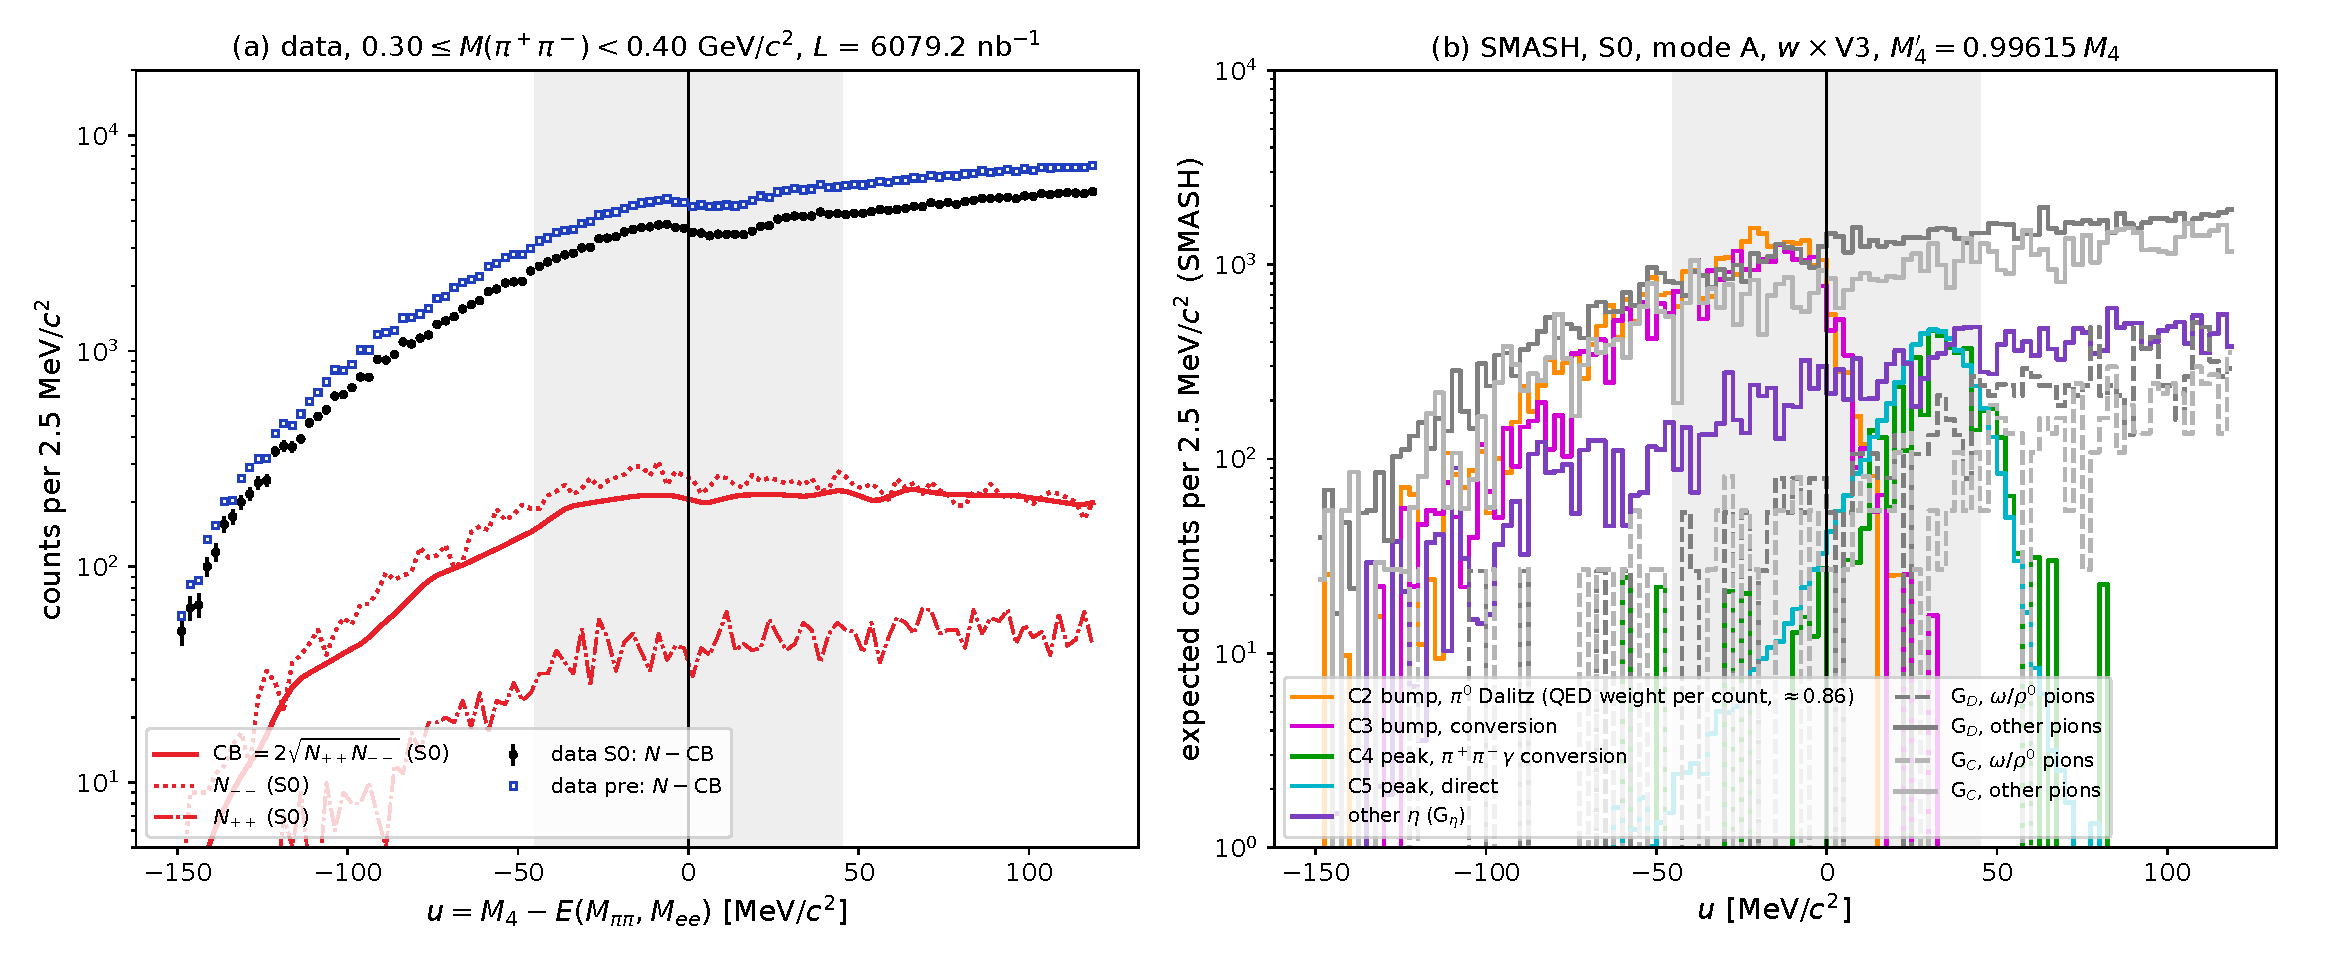
\includegraphics[width=\textwidth]{figs_all/edgeu_spectra_v3.pdf}
\caption{\textbf{What it shows: in $u$ the data show one edge at $u=0$ and the peak at $u=+20$ to $+55$\,\MeVcc; in SMASH the bump classes end at
$u=0$ and no other class has an edge there.}
Selection: (a) data, S0 (PT3 trigger, event vertex in the target region ($\vz>-160$\,mm), \betanew particle identification (pions within $3\sigma$, leptons within $5\sigma$ and with a RICH ring), energy-loss-corrected momenta of all four tracks, all stored combinations of each event (isBest $\ge0$), both pions in the event-vertex fit; black) and ``pre'' (without the pion-vertex requirement; blue squares); $0.30\le\Mpipi<0.40$\,\GeVcc, \Mee$<m_{\piz}=135$\,\MeVcc (where $u$ is defined); $u$ in 2.5\,\MeVcc bins, fit range $-45\le u<45$\,\MeVcc; CB $=2\sqrt{N_{++}N_{--}}$ of the like-sign data in 10\,\MeVcc cells of $u$ per \Mpipi slice (0.30--0.34, 0.34--0.37, 0.37--0.39, 0.39--0.40\,\GeVcc), $k=1$. (b) SMASH p+p at 4.5\,GeV (standard, lepton and $\eta$ sets, mode A) at its cross sections $\times$ PDG BR $\times$ the $\eta$-decay weights V3, masses moved to the data scale ($M_4'=0.99615\,M_4$, $\Mpipi'=0.9952\,\Mpipi$), S0 cuts, same \Mpipi and \Mee ranges.
(a) Data, $0.30\le\Mpipi<0.40$\,\GeVcc: $N-\mathrm{CB}$ for S0 (black) and ``pre'' (blue squares), CB $=2\sqrt{N_{++}N_{--}}$ (red), $N_{--}$ (red
dotted) and $N_{++}$ (red dash-dotted), per 2.5\,\MeVcc; grey band: the fit range. On this logarithmic scale the dip at $u=0$ and the $e^-e^-$ step
are hard to see; Fig.~\ref{fig:res-edgeu} and Fig.~\ref{fig:edgeu-checks}(d) show them. (b) SMASH (expected raw counts): C2 (per-count
QED weights, about 0.86) orange, C3 magenta, C4 green, C5 cyan, \Geta violet, $G_D$ dark grey, $G_C$ light grey (dashed: $\omega/\rho^0$ pions;
the greys are the reverse of Figs.~\ref{fig:res-after} and \ref{fig:edgeu-sim}).}
\label{fig:edgeu-spec}
\end{figure}

\subsection{The fit}
\label{sec:edgeu-fit}
\textbf{Model.} $N-\mathrm{CB}-\aP K(u)=\mathrm{pol2}(u)+h\,T(u)$, with $T$ the bin average of $\frac12\mathrm{erfc}(u/\sqrt2\sigma)$,
$\sigma=6.70$\,\MeVcc, and the variance cov(CB) + the model of $N$, iterated as in the per-slice fit. pol1 is rejected at every range of at
least $\pm35$\,\MeVcc ($\chi^2=115.6/33$ at $\pm45$); pol2 describes $\pm35$ to $\pm55$\,\MeVcc with $p=0.47$--0.70 ($\pm60$: $p=0.15$; $\pm70$:
$p=0.03$); pol3 gives about the same $f$ (0.429) with an error 1.8 times larger, because the cubic term and the step are both odd around $u=0$. The
nominal range $\pm45$\,\MeVcc is the half range of the per-slice method; its lower end stays above $-57$\,\MeVcc, where the first bump boxes
($m=0.40$) end, and its upper end below the region where pol2 starts to fail. $f$ is stable over $\pm40$ to $\pm55$\,\MeVcc (0.426--0.435).

\textbf{Result} (Fig.~\ref{fig:res-edgeu}). $h_{\mathrm{data}}=1305.2\pm62.3$ counts per 2.5\,\MeVcc, $\chi^2=27.3/32$ (466.6 without the step,
$\Delta\chi^2=439$, 21$\sigma$). $h_{\mathrm{sim}}=3065.8$ (C2 1738.8 with the per-count QED weights of D38, 2020.1 without them; C3 1327.0; C2 makes
57\,\% of the step). $f_\eta(u\text{-edge})=0.4257$, stat 0.0203 (fit) and 0.0199 (bootstrap), MC 0.0300 (replica rms; robust 0.0257); uncorrected
0.3900 (0.0182, 0.0267); with the conversions $\times0.48$ 0.5494. With \aP free the fit gives $\aP=0.33$ and the same $f$; \aP$\pm0.08$ moves $f$ by
0.02\,\% (3.86 counts of step per unit of \aP). The \emph{shape} of the peak term matters, through its low-mass tail (\S\ref{sec:edgeu-tail}, D40). The free step width in the data is $7.02\pm0.79$\,\MeVcc, against $6.42\pm0.86$\,\MeVcc for the same
fit on the SMASH Asimov spectrum; together with the peak width (data/SMASH $0.893\pm0.099$) the data/SMASH resolution ratio is $0.97\pm0.08$, so
the equal smearing is kept and the ratios 0.89 / 1.10 give the systematic. The smooth part also absorbs the slope of the bump below the edge
(SMASH C2+C3 rises by a factor of about 1.9 between $-44$ and $-14$\,\MeVcc): only the step height is a physical quantity.

\textbf{Per slice and per class.} Fitted separately (one pol2 per slice), the four slices give $f=\sum h_{\mathrm{data}}/\sum h_{\mathrm{sim}}=
0.4289\pm0.0201\pm0.0316$, the same as the single fit; the single fit itself adds nothing, the gain comes from the alignment on the edge and from
the bump-only simulated step.
\begin{center}\small
\resizebox{\textwidth}{!}{%
\tabin{edgeu_slices_v3.tex}}
\end{center}
The slices agree ($\chi^2=1.0/3$ with stat $\oplus$ MC; 9.4/3 with stat only). The step in $u$ per slice is about 13\,\% higher than the \Mfour step
of the per-slice edge (sum 1295 against 1142 counts), because it is sharper and the template width differs (6.7 against 5.4\,\MeVcc); the ratio to
SMASH is what counts. The E1/E2 split, $h_{\mathrm{data},i}=a(\mathrm{C2c}_i+\kappa\,\mathrm{C3}_i)$, gives $a_D=0.459\pm0.047\pm0.064$ and
$\kappa=0.83\pm0.20\,(\mathrm{stat})\pm0.34\,(\mathrm{MC})$: it prefers about 0.8 but cannot exclude the peak value 0.48 (1.0$\sigma$, MC error
only); the per-slice edge gave $0.47\pm0.24\pm0.46$.

\subsection{The step of the \texorpdfstring{$e^-e^-$}{e-e-} like-sign counts: lepton pairs from the two \texorpdfstring{$\pi^0$}{pi0} photons (D39)}
\label{sec:edgeu-ls}
\inshort{the $e^-e^-$ like-sign counts step at the bump edge because they contain lepton pairs from the two different photons of the \piz in
$\eta\to\pipi\piz$; such pairs have exactly the bump edge, lie at large \Mee, and are seen mostly as $e^-e^-$ because soft $e^+$ are accepted less
often and because the Compton and knock-on electrons of the photons are negative only. The CB removes them from the unlike-sign counts as designed
(tested in the data). It is not a charge flip. No number of the report changes; the earlier caveat ``$f$ up to 8\,\% higher'' is withdrawn (D39,
approved by the analyst on 15 November 2026). An independent verifier confirmed the mechanism and every data number, and corrected four statements (included below).}

\textbf{What was seen.} The $e^+e^+$ counts show no step over all \Mee ($2.1\pm6.5$); the $e^-e^-$ counts show $73.5\pm15.7$ (4.7$\sigma$;
the verifier's own fit: $\chi^2=37.1/32$ with the step, 59.1 without). Through CB $=2\sqrt{N_{++}N_{--}}$ the subtracted CB carries 39 counts of
step, 3.0\,\% of $h_{\mathrm{data}}$ (33--37 counts with other CB cells). Two descriptions of the first note overstated what it showed: ``only for
\Mee$\ge10$\,\MeVcc'' mostly reflects that 91.5\,\% of the $e^-e^-$ counts in the fit range lie there (an even share would put 6 counts in E1; the
observed $-6\pm5$ is 2.6$\sigma$ below); ``mostly in period I'' (I $50.8\pm10.8$, IIA $1.0\pm3.9$, IIB $7.3\pm6.9$, III $14.7\pm8.2$) is not
significant: against a share proportional to $L$, $\chi^2=4.9/3$, $p=0.18$. The first note read the size of the step (about 30\,\% of the
$e^-e^-$ counts per bin near $u=0$, against about 36\,\% for the bump in the unlike-sign counts) as bump events in the like-sign sample, possibly
through a wrong charge sign of the Dalitz $e^+$, with $f$ up to about 8\,\% higher. The study below (package eestep) replaces that reading.

\textbf{How it was studied.} Every like-sign entry (37\,835 $e^+e^+$, 127\,656 $e^-e^-$, ``pre'', $0.26\le\Mpipi<0.46$\,\GeVcc) and the
385\,800 unlike-sign entries of the edge region were joined to their PAT entries (all 551\,291 entries: momenta identical), which adds the track
quality of each lepton and the lepton and hadron multiplicities of the event. The three hypotheses of one event ($e^+e^-$, $e^+e^+$, $e^-e^-$)
were linked by an event key made of the run number, the event counter, the START time, the vertex $z$ and the total multiplicity (the counter
alone is not unique); every key is one block of adjacent entries (0 exceptions in 29 days $\times$ 3 trees). A ``twin'' of an $e^-e^-$ entry is an
$e^+e^-$ entry of the same event with the same $\pi^+$, $\pi^-$ and one of the two $e^-$. The simulation was dumped with the same logic and its
truth, and only used to identify the mechanism (no $k$ or CB number is taken from it). Estimators: those of the $u$-edge (\S\ref{sec:edgeu-fit};
the edgeu numbers $73.5\pm15.7$, $2.1\pm6.5$, $h_{\mathrm{data}}=1305.2$, $f=0.4200$ and the CB step 39.2 are reproduced exactly).

\textbf{The mechanism: pairs from the two photons of the \piz.} In $\eta\to\pipi\piz$, $\piz\to\gamma\gamma$ or $\gamma e^+e^-$, a pair can be formed
by leptons of the two \emph{different} photons: a Dalitz $e^\pm$ and a conversion $e^\pm$ of the other photon, or one conversion lepton of each
photon (``cross-photon pairs''; SMASH class T4, ``different sources'', which the analysis leaves to the CB). If photon 1 (energy $E_1$ in the $\eta$
frame) gives a lepton with the fraction $x_1$ of its four-momentum and photon 2 one with $x_2$, then $\Mee^2=x_1x_2m_{\piz}^2$ and
$M_4^2=m_\eta^2-2m_\eta[(1-x_1)E_1+(1-x_2)E_2]+(1-x_1)(1-x_2)m_{\piz}^2$. At fixed \Mee the largest $M_4$ is reached for $x_2=1$ and
$E_1=(E_0-p_0)/2$ ($E_0$, $p_0$: energy and momentum of the \piz): $m_\eta^2-m_\eta(E_0-p_0)(1-\Mee^2/m_{\piz}^2)$, which is the bump edge
$E(\Mpipi,\Mee)$ of \code{defs.h} (before its scale 0.99274). A toy with $4\times10^5$ decays per topology confirms it: the true $u$ never exceeds
0 (largest values $-0.0055$ and $-0.016$\,\MeVcc for two conversions and for Dalitz $+$ conversion), and the pairs within 5\,\MeVcc of the edge
are heavy (median \Mee 121 and 113\,\MeVcc).

\textbf{The data show exactly this} (Figs.~\ref{fig:res-eestep}, \ref{fig:eestep-spec}, \ref{fig:eestep-align}; S0, $0.30\le\Mpipi<0.40$\,\GeVcc,
step in counts per 2.5\,\MeVcc; the CB of each band from that band's own like-sign counts):
\begin{center}\small
\begin{tabular}{@{}l r r r r r r@{}}
\toprule
\Mee [\MeVcc] & $e^+e^+$ & $e^-e^-$ & $N$ & CB & $N-\mathrm{CB}$ & SMASH $\times f$ \\
\midrule
0--10 & $1.3\pm1.3$ & $-5.4\pm4.6$ & 683.6 & 2.6 & $681.0\pm43.5$ & 698.7 \\
10--30 & $-1.7\pm1.4$ & $4.2\pm5.8$ & 422.7 & $-1.1$ & $423.8\pm33.9$ & 363.6 \\
30--50 & $-0.4\pm1.9$ & $4.7\pm5.0$ & 103.3 & $-0.5$ & $103.8\pm17.1$ & 113.2 \\
50--70 & $-2.6\pm2.6$ & $10.1\pm6.1$ & 52.3 & $-0.1$ & $52.4\pm14.1$ & 78.1 \\
70--90 & $-2.0\pm3.0$ & $3.0\pm6.7$ & 30.0 & 2.8 & $27.2\pm12.4$ & 37.8 \\
90--110 & $7.6\pm3.2$ & $28.8\pm6.7$ & 31.1 & 22.9 & $8.2\pm10.3$ & 10.9 \\
110--135 & $-0.2\pm2.9$ & $27.3\pm6.1$ & 19.7 & 12.8 & $6.9\pm9.2$ & 3.5 \\
\midrule
0--50 & $-0.7\pm2.7$ & $3.6\pm8.9$ & 1209.7 & 0.2 & $1209.4\pm57.7$ & 1176.0 \\
90--135 & $7.3\pm4.3$ & $57.0\pm9.1$ & $52.6\pm10.9$ & $35.8\pm8.6$ & $16.8\pm13.9$ & 15.0 \\
70--135 & $5.1\pm5.3$ & $60.1\pm11.3$ & $83.8\pm15.2$ & $40.0\pm10.7$ & $43.8\pm18.6$ & 52.4 \\
\bottomrule
\end{tabular}
\end{center}
The last column is the expected bump signal (SMASH C2+C3 times $f$), a signal prediction, not a like-sign or CB rate. It was computed per band
with the constant C2 factor of D35 and $f=0.420$; with the per-count weights of D38 and $f=0.426$ the sums become 16.9 (90--135) and 54.6
(70--135) (\code{eestep_band_v3.log}); the single bands were not recomputed.
\begin{itemize}\setlength{\itemsep}{1pt}
\item \textbf{Large \Mee.} The $e^-e^-$ step is $57.0\pm9.1$ counts (6.3$\sigma$) at \Mee$\ge90$\,\MeVcc, $13.0\pm9.1$ at 50--90\,\MeVcc and
      $3.6\pm8.9$ (none) below 50\,\MeVcc, where 90\,\% of the bump lies. Opening angle of the two $e^-$: $-8.1\pm7.1$ counts at 0--10$^\circ$,
      $9.1\pm6.0$ at 10--20$^\circ$, $25.1\pm8.7$ at 20--35$^\circ$, $40.9\pm8.5$ at 35--60$^\circ$, $5.9\pm3.3$ above; the bump step of $N$ is at
      0--10$^\circ$ (1170 of 1349 counts).
\item \textbf{Tied to the edge with its \Mee term} ($e^-e^-$, \Mee$\ge70$\,\MeVcc; Fig.~\ref{fig:eestep-align}): $\Delta\chi^2$ of the step 28.3 in
      $u$, 0.5 in $\Mfour-E(m,0)$ (no \Mee term), 10.3 at a fixed $\Mfour=0.535$\,\GeVcc ($\chi^2=60/32$), 3.5 and 19.8 with the edge moved by
      $-10$ and $+10$\,\MeVcc. A free step position gives $u_0=-2.5$\,\MeVcc ($u_0=0$: $+2.0$ in $\chi^2$; $+5$\,\MeVcc: $+13.4$); the width is not
      constrained. Per \Mpipi slice it grows toward the high slice ($8.7\pm6.7$, $17.8\pm6.4$, $30.9\pm6.4$). In the control region
      \Mpipi 0.42--0.46\,\GeVcc, where the decay is impossible, there is none ($-2.0\pm3.1$). This is also why the per-slice edge (which uses
      $E(m,0)$) and Part~II's like-sign edge test in \Mfour ($0.5\pm25.6$ counts for ``pre'') see no like-sign step: at large \Mee the true edge lies
      far below $E(m,0)$, and the step is smeared out.
\item \textbf{Events without an $e^+$.} 85\,\% of the $e^-e^-$ counts near the edge come from events with no positive lepton at all and no $e^+e^-$
      combination; the step is in these events ($66.4\pm14.5$; no positive lepton: $65.4\pm14.4$). Events with an $e^+e^-$ twin show none ($6.8\pm6.0$),
      nor do combinations whose two $e^-$ share a RICH ring ($-2.7\pm4.7$) or events with three or more $e^-$ ($0.6\pm2.8$); isBest $=1$ / $=0$:
      $52.6\pm14.2$ / $20.9\pm6.5$.
\item \textbf{Ordinary tracks.} The share of step counts is flat in every track-quality variable (RK, inner and outer segment, META and RICH match,
      ring pads, $\beta$, momenta; $p=0.14$--0.99), in the sectors (0.30--0.47; sector 2: 0.39) and in the days ($p=0.26$). It is not flat only in
      \Mee ($p=0.01$; 0.04 below 89\,\MeVcc, 0.52--0.57 above) and somewhat in the polar angle ($p=0.06$), as expected for wide pairs.
\item \textbf{Why $e^-e^-$ and hardly $e^+e^+$.} Two reasons. The pairs contain soft leptons, and soft $e^+$ are accepted less often than
      soft $e^-$. And a photon can also give a Compton electron or a knock-on (delta) electron, which is always negative and has no $e^+e^+$
      counterpart; in SMASH part of the $e^-e^-$ cross pairs carry one (verifier). In the data at \Mee$\ge90$\,\MeVcc the $e^+e^+$ counts show
      $7.3\pm4.3$ of step, a ratio to $e^-e^-$ of $0.13\pm0.08$: the $e^+e^+$ counts have a small step too; ``no step'' over all \Mee was small
      numbers.
\end{itemize}

\textbf{The CB removes these pairs as designed.} Before acceptance a decay with a Dalitz or conversion pair on each photon gives one $e^-e^-$,
one $e^+e^+$ and two $e^+e^-$ cross pairs; a Compton or knock-on electron gives one $e^-e^-$ and one $e^+e^-$ pair and no $e^+e^+$. The $e^+e^-$
ones are in $N$, and CB $=2\sqrt{N_{++}N_{--}}$ is built to subtract them; with an acceptance that factorises per lepton the rule removes both
kinds to within a few per cent (expected $k$ between 0.96 and 1.02, depending on the share of Compton/knock-on legs; verifier). The model ``step of $N$ $=f\,h_{\mathrm{sim}}+k_{\mathrm{cross}}\,h(\mathrm{CB})$'' was tested at \Mee$\ge90$\,\MeVcc, where the
bump is small: $h(N)=52.6\pm10.9$, $h(\mathrm{CB})=35.8\pm8.6$, $N-\mathrm{CB}=16.8\pm13.9$ against the expected bump signal $f\,h_{\mathrm{sim}}=16.9$ ($z=-0.01$; with the
per-count C2 weights of D38; 15.0 with the constant factor of D35). If the like-sign step had no $e^+e^-$ partners (an artefact), $N-\mathrm{CB}$
would be $16.9-35.8=-19.0$; the data are 2.6$\sigma$ (statistical) from that. The scale of the cross pairs in $N$ relative to the CB rule, from
the data, is $k_{\mathrm{cross}}=1.00\pm0.39$ (1 = the CB rule). With \Mee$\ge70$\,\MeVcc: $43.8\pm18.6$ against 54.6 ($z=-0.58$; artefact
$z=1.57$), $k_{\mathrm{cross}}=0.73\pm0.43$. The bump prediction has an MC error of about $\pm6.7$ (17 simulated entries), which lowers the
artefact $z$ to about 2.3$\sigma$. The verifier's own construction, made with the constant C2 factor of D35, gives $h(N)=52.7\pm10.4$, CB
$39.6\pm9.8$, $N-\mathrm{CB}=13.1\pm14.6$ against $14.7\pm6.7$ (MC), $k_{\mathrm{cross}}=0.96\pm0.48$ ($\pm0.52$ with the MC error; scaled with
the per-count weights its prediction becomes about 16.3 and $k_{\mathrm{cross}}$ about 0.91); the artefact reading is 2.6$\sigma$ away in this
form, 3.7$\sigma$ from the step of $N$ alone (statistical) and 2.4--2.9$\sigma$ with the MC error. At this \Mee the
fixed peak term contributes a step of $-20.1$ counts (direct decays just above the edge); it changes no conclusion. With $k$ between 0.96 and 1.02,
$f$ is right to 0.13\,\%.

\textbf{Not a charge flip.} A Dalitz $e^+$ reconstructed as $e^-$ keeps its momentum, so the $e^-e^-$ combination would have the small \Mee and the $u$ of
the bump combination. Below 50\,\MeVcc the $e^-e^-$ step is $3.6\pm8.9$ counts against 1209.7 counts of bump step in $N$: flip rate $r=0.003\pm0.007$,
$r<1.24$\,\% (90\,\% CL). At that limit $f$ would be higher by less than 1.6\,\% (1.2\,\% of lost bump counts and 0.35\,\% of CB over-subtraction).
A flip of either charge gives less than 1.9\,\%, because an $e^+e^+$ excess enters the CB $\sqrt{N_{--}/N_{++}}=3.25$ times (verifier: $e^-\to e^+$
rate $-0.0006\pm0.0023$; negative copies of the $e^+$: $-4.8\pm3.1$ counts).
Unlike-sign combinations with an $e^-e^-$ twin (a wrong-sign copy of the $e^+$) show no step ($-4.1\pm7.4$; clone rate $-0.003\pm0.006$). In the
simulation a true $e^+e^-$ pair appears as a like-sign entry in 0.04\,\% (standard set), 0.01\,\% (lepton set) and 0.008\,\% ($\eta$ set) of
the cases; per true $e^+$, a negative charge is reconstructed for 1.7\,\% below 100\,MeV$/c$, 0.46\,\% at 100--200, 0.10\,\% at 200--300 and at
most 0.06\,\% above.

\textbf{Effects on the measurements} (no number of the report changes):
\begin{center}\small
\begin{tabularx}{\textwidth}{@{}>{\raggedright\arraybackslash}p{2.6cm} >{\raggedright\arraybackslash}p{2.2cm} L L >{\raggedright\arraybackslash}p{3.4cm}@{}}
\toprule
quantity & nominal (CB rule, supported) & $k_{\mathrm{cross}}$ from the data & charge flip (90\,\% CL limit) & artefact reading (disfavoured, 2.3--3.7$\sigma$) \\
\midrule
$f_\eta(u\text{-edge})$ 0.426 & unchanged & $0.0\pm1.2$\,\% (\Mee$\ge90$); $+0.8\pm1.3$\,\% ($\ge70$); inside U5 (2.6\,\%) & $<+1.6$\,\% ($e^+$ flip); $<+1.9$\,\% (either charge) & $+3.0$\,\% (CB step of 39.2 counts removed) \\
$f_\eta(\mathrm{edge})$ 0.423 & unchanged & inside its E4 variant ($+1.3$\,\%) & $<+1.6$\,\% & same order (not computed) \\
\Ypeak 5088 & unchanged & -- & -- & $-0.7$\,\% (P only) / about $+1.9$\,\% (with the side bands at $R'=1$; first estimate $+3.0$\,\% with 255 side-band pairs) \\
X17 limit ($r$ and BR$\times$BR) & unchanged & -- & -- & none (out of reach) \\
\bottomrule
\end{tabularx}
\end{center}
The cross pairs reach the peak window P only at \Mee$\ge101.5$, 104.0, 110.5 and 119.5\,\MeVcc for \Mpipi $=0.28$, 0.30, 0.35 and 0.40\,\GeVcc.
With the cross-pair share of the $e^-e^-$ counts just below the edge ($0.56\pm0.09$, \Mee$\ge90$\,\MeVcc) there are about 180 of them in the lower
side band (0.5250--0.5336\,\GeVcc; the first count, 255, was for the wider range 0.5225--0.5336) and about 50 in P, carrying 37 CB counts (none in
the upper side band); with their partners they are subtracted and \Ypeak is unchanged (with the expected $k$ the residual in P is below 1.5
counts, 0.03\,\%; the share is measured at the edge in 0.30--0.40\,\GeVcc only, so these window numbers are estimates). For \Mee$\le24.5$\,\MeVcc
the edge is at most 0.5211--0.5223\,\GeVcc, 11.4--12.5\,\MeVcc (about 1.8$\sigma$ of the $u$ resolution) below P: none of the 207 $e^-e^-$ and 13 $e^+e^+$ counts of the X17P window can be a
cross pair, and the $e^-e^-$ step at 10--30\,\MeVcc is $4.2\pm5.8$. The CB variants of the $u$-edge bracket all readings: CB shape from $e^+e^+$
only $+1.1$\,\%, from $e^-e^-$ only $-1.3$\,\%, CB $=N_{++}+N_{--}$ $-2.6$\,\%; family U5 counts 2.6\,\%.

\textbf{What the simulation contributes.} The simulation does not model the like-sign or combinatorial background, so its like-sign entries
are used only to identify the origin: in the standard set (the only one with $\eta\to\pipi\piz$) SMASH contains such cross pairs, mostly
$e^-e^-$, at large \Mee (around 100\,\MeVcc) and wide opening angles (around 40$^\circ$). No SMASH like-sign number enters a correction or the CB,
and no like-sign rate of the data is compared with the simulation; the CB comes from the data, and $k_{\mathrm{cross}}$ shows that the partners are
there. Pairs merged into one track (a whole photon in one lepton) are not seen (no excess of large rings or of double energy loss in the step
counts).

\notebox{\textbf{D39} (lead analysis, approved by the analyst on 15 November 2026; no headline number changes). (1) Record the origin: the step
of the $e^-e^-$ like-sign counts at $u=0$ is made of lepton pairs from the two photons of the \piz in $\eta\to\pipi\piz$ (cross-photon pairs),
with the same kinematic edge as the bump, at \Mee$\ge90$\,\MeVcc, seen mostly as $e^-e^-$ because of the $e^+$/$e^-$ acceptance and of
Compton/knock-on electrons (negative only; data $e^+e^+/e^-e^-=0.13\pm0.08$); not a charge flip ($r<1.2$\,\%, 90\,\% CL). (2) Keep the nominal CB
$=2\sqrt{N_{++}N_{--}}$ and U5 (2.6\,\%) as they are; the data test supports the CB rule ($k_{\mathrm{cross}}=1.00\pm0.39$ with the per-count C2
weights; independent, with the constant factor, $0.96\pm0.48$; the artefact reading is disfavoured at 2.6$\sigma$ statistical, about 2.3$\sigma$
with the MC error). (3) In all three parts, replace the caveat ``$f$ up to about 8\,\% higher'' by the flip limit ($<+1.6$\,\% on $f$,
$<+1.9$\,\% for either charge, 90\,\% CL) and the $k_{\mathrm{cross}}$ check ($0.0\pm1.2$\,\%, covered by U5, not a new term). (4) Correct ``the
$e^+e^+$ counts have no step'' to: the $e^+e^+$ counts have a small step too ($7.3\pm4.3$ at \Mee$\ge90$\,\MeVcc); the ``30\,\% against 36\,\%''
argument is void, because the $e^-e^-$ step lives where the bump is small. \emph{Independently verified} (wording corrected; no number changes).}

\textbf{Checks and limits.} Self-checks of the package: the edgeu numbers reproduced exactly; the PAT join and the event keys without
exception (data and simulation; 238\,040 simulated like-sign entries identical in both dumps). The $k_{\mathrm{cross}}$ test relies on the expected bump
signal SMASH $\times f$ at \Mee$\ge90$\,\MeVcc (16.9 counts with the per-count C2 weights, from 17 simulated entries); the window estimates rely
on a share measured at the edge; no SMASH number is used for a correction or the CB. Bands above 50\,\MeVcc are outside the blinded X17 region;
in the X17P window the like-sign counts were only counted.

\textbf{Verification} (veestep, own code: a new data dump with its own PAT joins, an own Poisson-likelihood step estimator, an own CB
construction and bootstrap, an own kinematic toy and an own reading of the simulated like-sign entries; no eestep code or output used).
\emph{Verdict: CONFIRMED WITH CORRECTIONS.} A general proof shows that any pair made of \piz decay products, with the rest lost, cannot pass
$E(\Mpipi,\Mee)$ (the maximum is the two-body decay into the pair and a massless particle); the own toy (600\,000 decays per pair type) never
exceeds $u=0$ and predicts that the density of cross pairs falls in the last 5--10\,\MeVcc below the edge, so that after the resolution the step
sits at $u=-2.5$\,\MeVcc, exactly where the data put it (the bump classes: at 0). The same 1\,910\,080 entries as edgeu give the same steps
($e^-e^-$ $73.5\pm15.6$, $e^+e^+$ $2.1\pm6.5$; \Mee$<50$: $3.6\pm8.9$; $\ge90$: $57.0\pm9.0$; ratio $0.127\pm0.079$), the same opening angles
(20--35$^\circ$: $25.1\pm8.7$; 35--60$^\circ$: $40.8\pm8.5$), the same event content (85.0\,\% without a positive lepton; every key one block of
adjacent entries, 0 exceptions in 29 days) and $f=0.4193$. Corrections, all included above: the Compton and knock-on electrons (why $e^-e^-$,
and the pair bookkeeping), the size of the CB test (2.7$\sigma$ is statistical; $k_{\mathrm{cross}}$ about $\pm0.5$), and two numbers (either-charge flip $<1.9$\,\%; about 180 cross
pairs in the lower side band, not 255). A new test finds no merged conversion pairs (no excess of large rings or double energy loss in the
step counts). \Ypeak and the X17 limit are not touched.

\begin{figure}[!htbp]
\centering
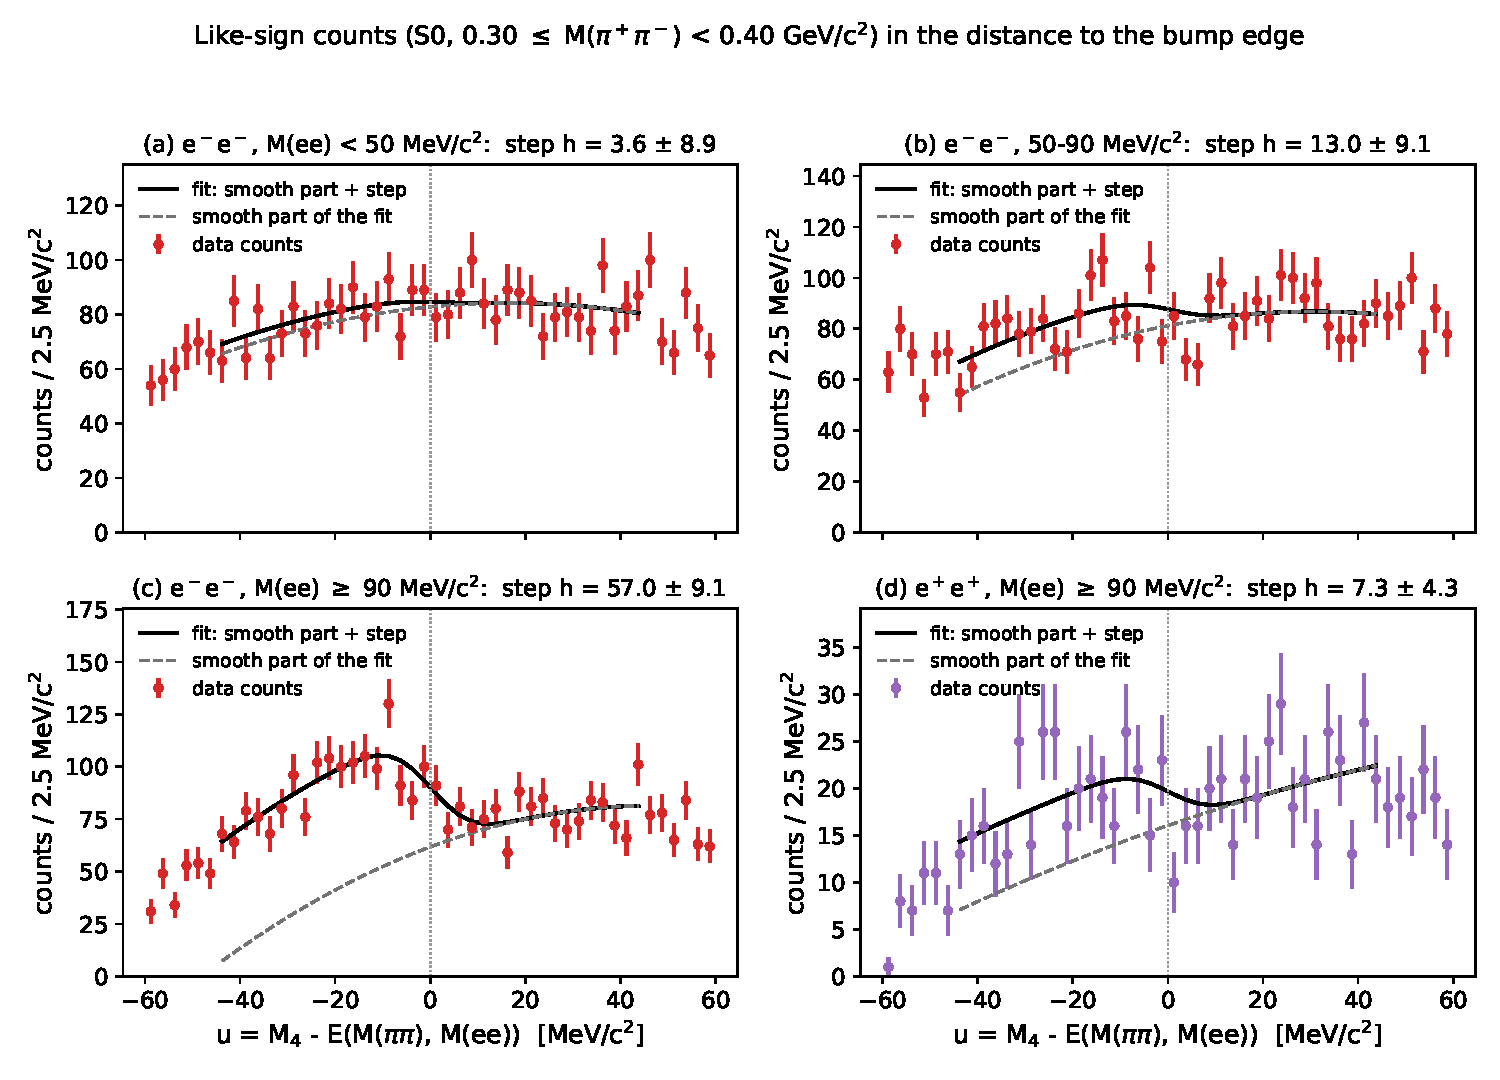
\includegraphics[width=0.95\textwidth]{figs_all/eestep_spectra_cnt.pdf}
\caption{\textbf{What it shows: the like-sign counts have no step at the bump edge below \Mee$=50$\,\MeVcc, where the bump lies, and a clear step
at \Mee$\ge90$\,\MeVcc, where the pairs from the two \piz photons lie, in $e^-e^-$ and (smaller) in $e^+e^+$.}
Selection: data, S0 (PT3 trigger, event vertex in the target region ($\vz>-160$\,mm), \betanew particle identification (pions within $3\sigma$, leptons within $5\sigma$ and with a RICH ring), energy-loss-corrected momenta of all four tracks, all stored combinations of each event (isBest $\ge0$), both pions in the event-vertex fit); $0.30\le\Mpipi<0.40$\,\GeVcc; like-sign counts only (no CB subtraction): $\pi^+\pi^-e^-e^-$ with \Mee 0--50, 50--90, 90--135\,\MeVcc (a--c), $\pi^+\pi^-e^+e^+$ with \Mee 90--135\,\MeVcc (d); $u$ in 2.5\,\MeVcc bins, fit range $-45\le u<45$\,\MeVcc.
Data S0, $0.30\le\Mpipi<0.40$\,\GeVcc, counts per 2.5\,\MeVcc in $u=\Mfour-E(\Mpipi,\Mee)$. (a) $e^-e^-$, \Mee$<50$\,\MeVcc: $3.6\pm8.9$;
(b) $e^-e^-$, 50--90\,\MeVcc: $13.0\pm9.1$; (c) $e^-e^-$, \Mee$\ge90$\,\MeVcc: $57.0\pm9.1$; (d) $e^+e^+$, \Mee$\ge90$\,\MeVcc: $7.3\pm4.3$.
Points: data counts; black line: the nominal fit (smooth part $+$ step, $\pm45$\,\MeVcc); grey dashed: the smooth part of the same fit (it also
absorbs the slope below the edge; it is not ``the background''). Package eestep.}
\label{fig:eestep-spec}
\end{figure}

\begin{figure}[!htbp]
\centering
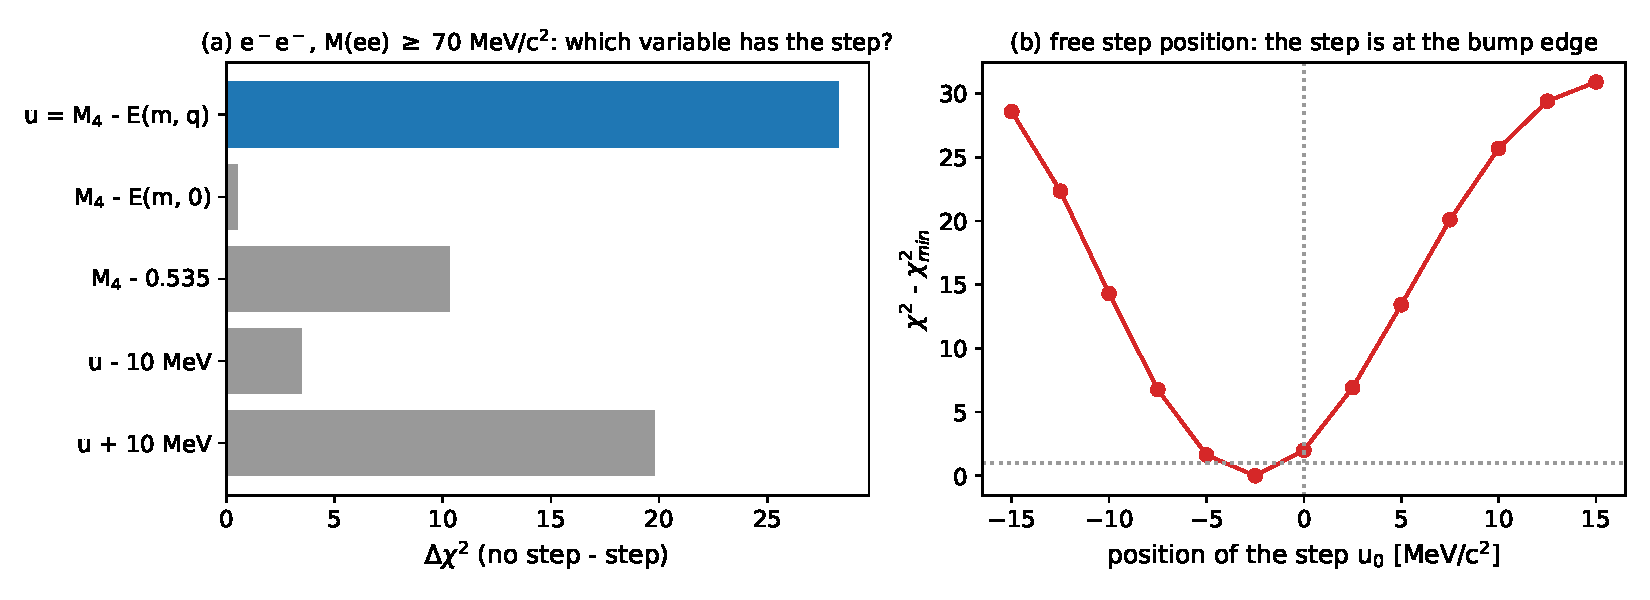
\includegraphics[width=0.95\textwidth]{figs_all/eestep_align.pdf}
\caption{\textbf{What it shows: the $e^-e^-$ step is tied to the edge $E(\Mpipi,\Mee)$ of $\eta\to\pipi\piz$, including its \Mee term, and sits
at $u=0$; it is not a fixed structure in \Mfour.}
Selection: data, S0 (PT3 trigger, event vertex in the target region ($\vz>-160$\,mm), \betanew particle identification (pions within $3\sigma$, leptons within $5\sigma$ and with a RICH ring), energy-loss-corrected momenta of all four tracks, all stored combinations of each event (isBest $\ge0$), both pions in the event-vertex fit); $\pi^+\pi^-e^-e^-$ counts with \Mee 70--135\,\MeVcc and $0.30\le\Mpipi<0.40$\,\GeVcc; each variable in 2.5\,\MeVcc bins, pol2 + a step (smeared by 6.7\,\MeVcc) fitted over $\pm45$\,\MeVcc.
Data S0, $e^-e^-$ counts with \Mee$\ge70$\,\MeVcc, $0.30\le\Mpipi<0.40$\,\GeVcc. (a) $\Delta\chi^2$ between the fits without and with a step for
five variables: $u$ (28.3), $\Mfour-E(m,0)$ without the \Mee term (0.5), a fixed $\Mfour-0.535$\,\GeVcc (10.3), and the edge moved by $-10$ and
$+10$\,\MeVcc (3.5, 19.8). (b) $\chi^2-\chi^2_{\min}$ against the position $u_0$ of the step: minimum at $-2.5$\,\MeVcc, $u_0=0$ is $+2.0$; dotted:
$\Delta\chi^2=1$. Package eestep.}
\label{fig:eestep-align}
\end{figure}

\subsection{The low-mass tail of the \texorpdfstring{$\eta$}{eta} peak term (D40)}
\label{sec:edgeu-tail}
\inshort{the simulated $\eta$ peak has a low-mass tail: in about a quarter of its entries a lepton lost momentum in the detector material
(HGeant); the generator itself writes a sharp line. In $u$ this tail reaches the bump edge, so its size changes the fitted step:
$f_\eta(u\text{-edge})$ moves by $+6.8$\,\% per unit of the tail size $t$ ($t=1$: SMASH as it is; $t=0$: no tail), the per-slice edge by
$+7.3$\,\%, \aP and \sigeta from the peak side bands by $+17.7$\,\%. The data cannot measure $t$ ($0.3\pm1.0$). Physics says the tail is there,
and the radiation of the decay itself, which SMASH lacks, would make it about 10\,\% larger. Approved by the analyst on 15 November 2026
(D40, option (a)): $t=1$ is kept and a term for $t=1\pm0.5$ is counted: $\pm3.4$\,\% on $f_\eta(u\text{-edge})$, $\pm3.6$\,\% per slice (3.7\,\%
with the per-count C2 weights), $\pm8.8$\,\% on \sigeta from the peak, which becomes $0.43\pm0.17\,(\mathrm{measurement})$\,mb.}

\textbf{Why it matters, in plain words.} The $u$ fit subtracts the $\eta$ peak as a fixed SMASH term $\aP K(u)$ (\S\ref{sec:edgeu-fit}). Most of
the peak lies at $u=+20$ to $+55$\,\MeVcc, well above the edge. But some peak combinations have a lower mass than they should, because a lepton lost part
of its momentum on its way through the detector; these form a tail of the peak towards low \Mfour, and in $u$ this tail reaches the edge at
$u=0$. The \emph{size} of the peak term hardly matters, because its core and its tail push the fitted step in opposite directions and cancel
($+162$ and $-158$ counts of step per unit of \aP; the net 3.86 of \S\ref{sec:edgeu-fit}); if only the tail changes, the cancellation breaks.

\begin{figure}[!tb]
\centering
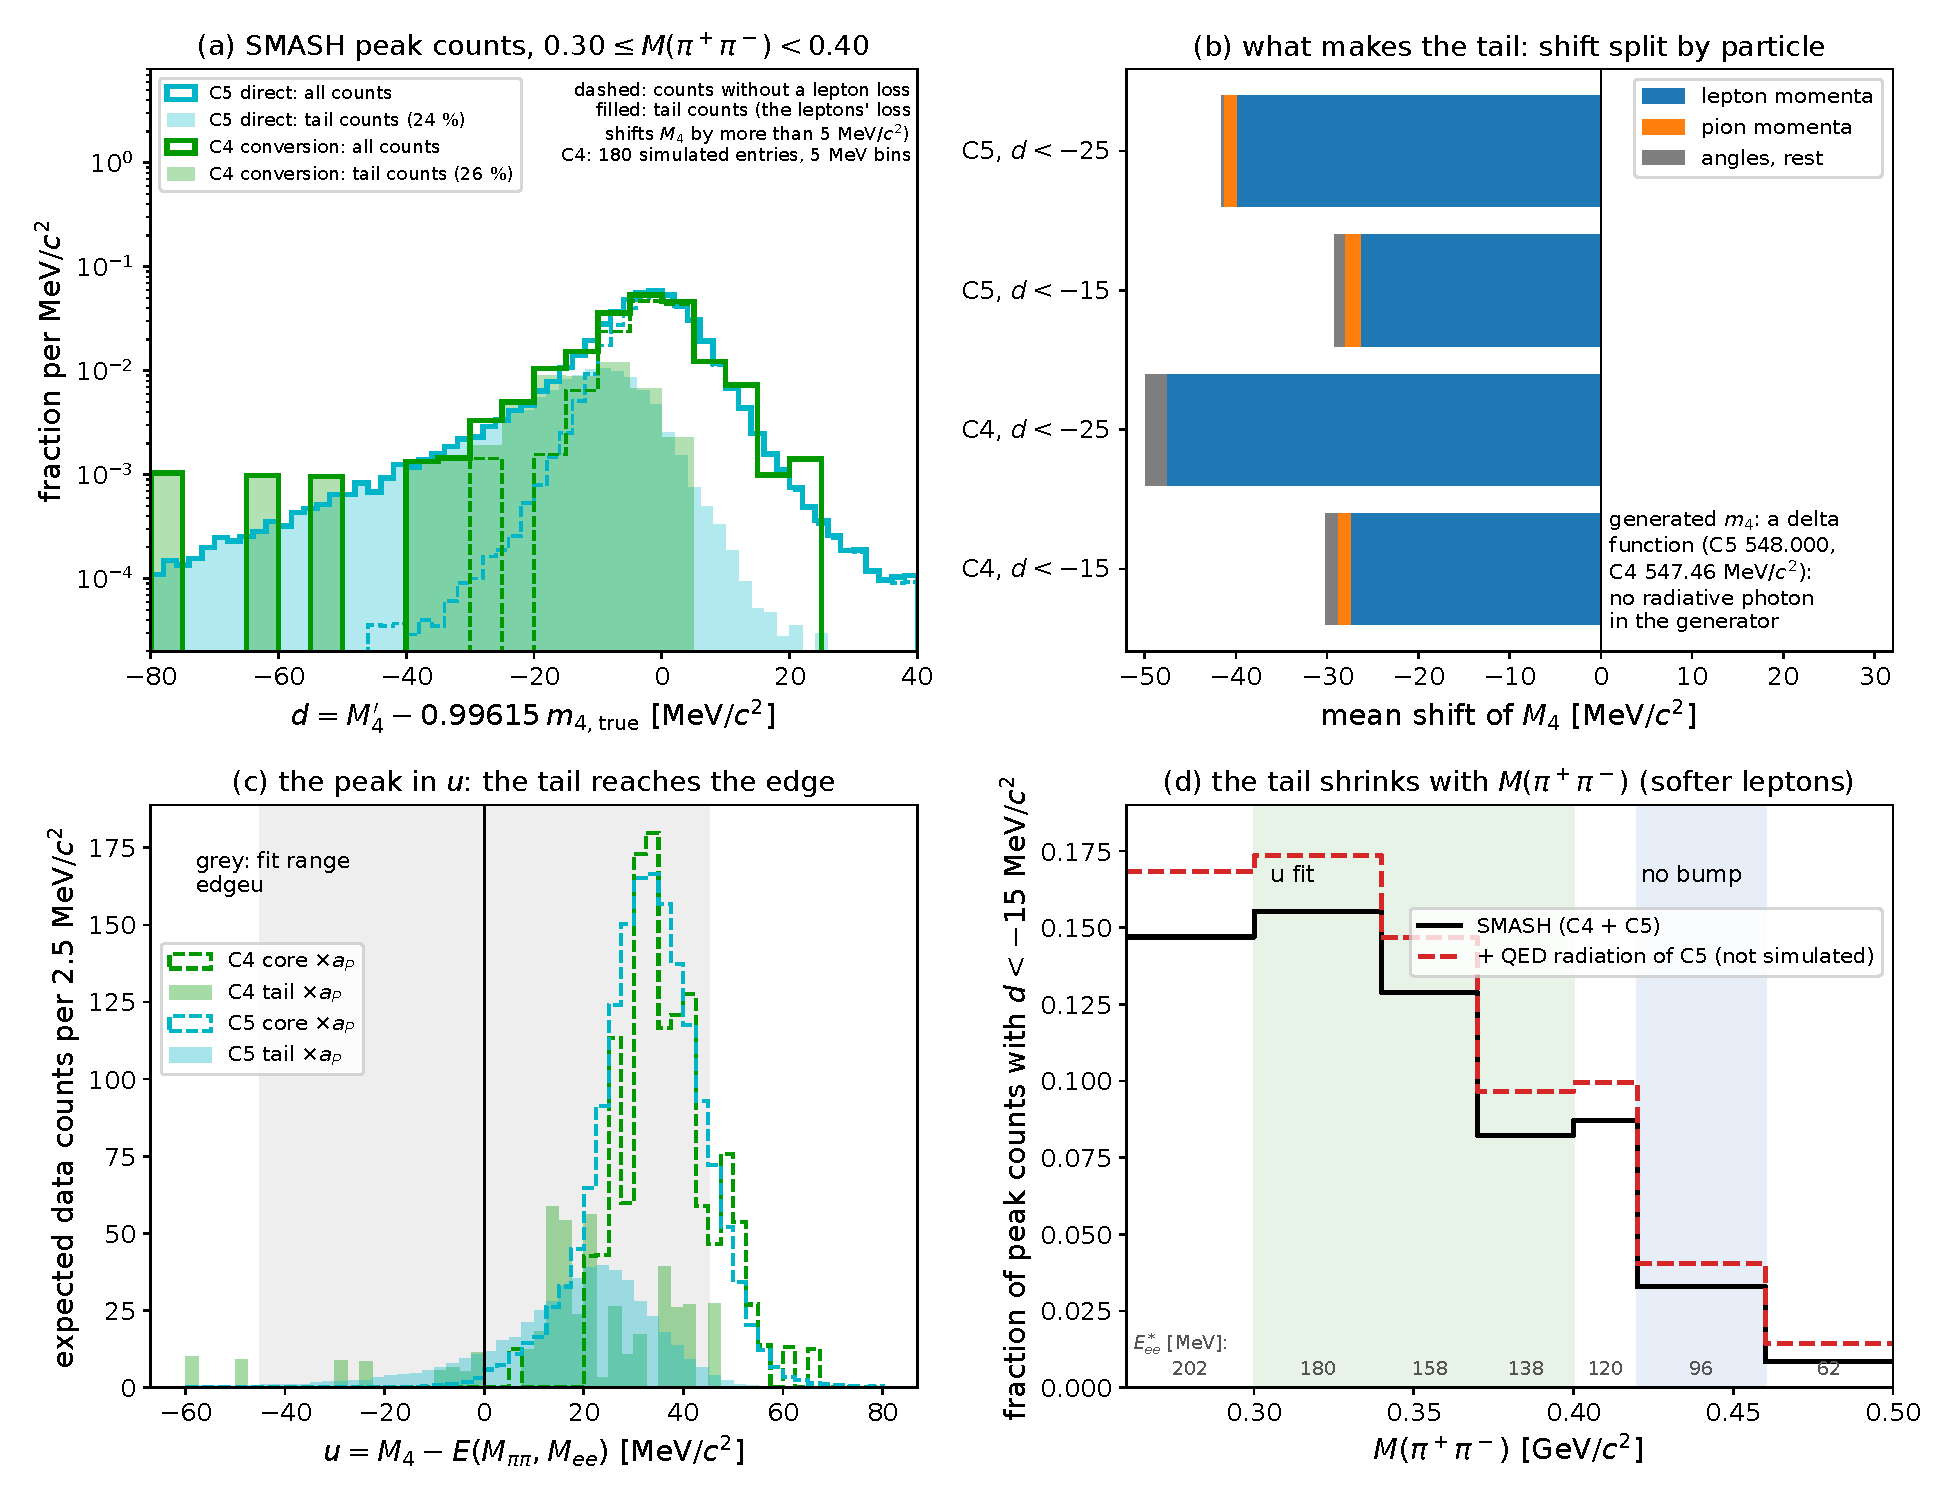
\includegraphics[width=0.86\textwidth]{figs_all/peaktail_sources_cnt.pdf}
\caption{\textbf{What it shows: the tail of the simulated $\eta$ peak comes from the leptons' momentum loss in the detector material, not from the
generator; in $u$ it reaches the bump edge, and it shrinks at large \Mpipi.}
Selection: simulation only: the $\eta$ peak classes C4 and C5 of SMASH p+p at 4.5\,GeV (standard, lepton and $\eta$ sets, mode A) at its cross sections $\times$ PDG BR $\times$ the $\eta$-decay weights V3, masses moved to the data scale ($M_4'=0.99615\,M_4$, $\Mpipi'=0.9952\,\Mpipi$), S0 cuts (PT3 trigger, event vertex in the target region ($\vz>-160$\,mm), \betanew particle identification (pions within $3\sigma$, leptons within $5\sigma$ and with a RICH ring), energy-loss-corrected momenta of all four tracks, all stored combinations of each event (isBest $\ge0$), both pions in the event-vertex fit); $0.30\le\Mpipi'<0.40$\,\GeVcc in (a)--(c); (d) $\Mpipi'$ bins 0.26--0.30, 0.30--0.34, 0.34--0.37, 0.37--0.40, 0.40--0.42, 0.42--0.46, 0.46--0.50\,\GeVcc.
SMASH, S0, $0.30\le\Mpipi<0.40$\,\GeVcc unless stated. (a) Residual $d=M_4'-0.99615\,m_4^{\mathrm{true}}$ of the simulated peak counts: direct decays C5
(cyan) and conversions C4 (green, 180 simulated entries, 5\,\MeVcc bins); solid: all counts; filled: tail counts (the leptons' loss shifts \Mfour
by more than 5\,\MeVcc; 24 and 26\,\%); dashed: the other counts, symmetric. (b) Mean shift of \Mfour of the counts with $d<-15$ and $<-25$\,\MeVcc, split into
lepton momenta (blue), pion momenta (orange) and angles and the rest (grey); the generated $m_4$ is a sharp line (linearised split; the
verifier's substitution of the true momenta gives a lepton share 2--3\,\MeVcc smaller, the same conclusion). (c) The peak in $u$ in expected data
counts $\times\aP=0.418$ per 2.5\,\MeVcc: core counts (dashed) and tail counts (filled); grey: the $u$-fit range. (d) Share of peak counts with
$d<-15$\,\MeVcc per \Mpipi bin: SMASH (black) and SMASH with the QED radiation of C5 that the generator lacks (red dashed, leading-log toy);
numbers: the \ee energy in the $\eta$ frame; shaded: the $u$-fit region and the region without bump. Package peaktail.}
\label{fig:edgeu-tail}
\end{figure}

\textbf{Where the tail comes from} (simulation, $0.30\le\Mpipi<0.40$\,\GeVcc; Fig.~\ref{fig:edgeu-tail}).
\begin{itemize}\setlength{\itemsep}{1pt}
\item \textbf{Not from the generator.} The true four-body mass of the direct decays (C5) is a sharp line: 547.998 / 548.000 / 548.002\,\MeVcc
      (quantiles 0.1 / 50 / 99.9\,\%; C4: 546.5 / 547.46 / 547.85). The converter of the simulation has no PHOTOS, its ``brems'' plugins are
      nucleon--nucleon bremsstrahlung, and its $\eta$ physics plugin is disabled: no radiative photon is generated.
\item \textbf{Not from the conversion itself.} The C4 pairs come from pair production of the photon (GEANT process 6 with a photon parent in all
      287 C4 entries) and carry the whole photon four-momentum ($m_4^{\mathrm{true}}$ within 1.5\,\MeVcc of 548\,\MeVcc for 99.9\,\% of them).
\item \textbf{From the leptons in the material.} The lepton momentum loss is one-sided ($p/p_{\mathrm{true}}<0.90$ for 7.0\,\% of the leptons,
      $>1.10$ for 0.7\,\%); bremsstrahlung in the material is the natural reading, modelled by HGeant. In entries shifted by more than $-25$\,\MeVcc
      the leptons make $-38$ of $-41$\,\MeVcc (C5) and $-45$ of $-48$\,\MeVcc (C4); the pions about $-2$\,\MeVcc.
\item \textbf{Its size.} 26\,\% of the C4 and 24\,\% of the C5 entries are tail entries (the leptons' loss shifts \Mfour by more than 5\,\MeVcc);
      entries without such a loss are symmetric (C5: 1.3\,\% below $-15$, 1.7\,\% above $+15$\,\MeVcc). The tail shrinks at large \Mpipi, where the
      leptons are softer (entries shifted by more than $-15$\,\MeVcc: 15.5\,\% at 0.30--0.34, 3.3\,\% at 0.42--0.46, 0.8\,\% at 0.46--0.50\,\GeVcc).
\item \textbf{Where it lies in $u$.} 87\,\% of the peak is inside the fit range; 17\,\% lies below $u=+20$\,\MeVcc (about 670 data counts), 73\,\% of
      them from tail entries; 197 counts (5\,\%) lie within 10\,\MeVcc of the edge, 70\,\% of them from tail entries.
\item \textbf{What SMASH lacks.} The radiation of the decay $\eta\to\ppee$ itself is not generated; a leading-log estimate makes the C5 tail
      16--19\,\% larger ($t\approx1.1$ for C4+C5).
\end{itemize}

\textbf{What the data say about the size.} With \aP fixed at 0.418 the $u$ fit with a free tail scale gives $t=0.47$--1.01 for five fit
choices ($\pm0.4$--0.5 each). But \aP is itself a measurement ($\pm0.080$) and depends on $t$ through the leakage of the peak into its side bands
(\aP$\times0.853$ at $t=0$, $\times1.209$ at $t=2$); with this constraint the same fit gives $t=-0.19$ to $0.12$ with the raw templates and $-0.01$
to $0.93$ with smoothed C4 entries, each with a $\Delta\chi^2=1$ interval of about $\pm0.9$--1.0. The line shape of the peak where no bump exists
($0.42\le\Mpipi<0.46$\,\GeVcc) does not help: there C4 is 49 heavy simulated entries (58\,\% of the peak; their bootstrap moves $t$ by 0.56--0.81),
and a peak shift of 1\,\MeVcc does the same as one unit of $t$ (shifts of $-2$ to $+2$\,\MeVcc give $t=-1.55$ to $+2.26$ at the same
$\chi^2$). Reading: $t=0.3\pm1.0$; the SMASH tail ($t=1$, 0.7$\sigma$ away) and no tail (0.3$\sigma$) are both allowed. The study's own
reading, $t=0.72\pm0.38$, ``no tail disfavoured at 1.9$\sigma$'' and ``the Gaussian check excluded at 2.6$\sigma$'', did not survive the
verification and is withdrawn. A peak without a tail is excluded by physics (the material exists, and the decay radiates), not by the data.

\textbf{How the results move with the tail} (Table~\ref{tab:edgeu-tail}): both edge measurements rise by about 7\,\% per unit of $t$,
the peak side bands by 18\,\%; the two edge methods move together, so ``they agree to 0.5\,\%'' stays.
\begin{table}[!tb]
\centering
\caption{\textbf{What it shows: how much the bump and peak results move with the size of the low-mass tail of the simulated $\eta$ peak, and the
term of D40 (approved, option (a)).} $t$ scales the tail entries of the SMASH peak term ($t=1$: SMASH as is); nominal values with the per-count C2
weights of D38. Errors of the nominal values as in
Table~\ref{tab:summary}; ``total (meas.)'' of \sigeta adds stat, syst, MC and the normalisation in quadrature. Packages peaktail and vpt
(\code{peaktail_numbers.json}, \code{vpt_*.json}); per slice with the D38 class factors, \code{peaktail_bedge_v3.txt}
(\code{edgeu_tail_v3.tex}).}
\label{tab:edgeu-tail}
\small
\tabin{edgeu_tail_v3.tex}
\end{table}
The $u$ fit itself has $\chi^2=27.1$ / 27.3 / 35.5 for $t=0$ / 1 / 2 (32 degrees of freedom). The QED radiation of C5 would add $+0.6$\,\%
($u$-edge), $+0.7$\,\% (per slice) and $+1.9$\,\% (\aP).

\textbf{The Gaussian check of the integration, taken apart.} Part~II's data-only peak term, a plain Gaussian (5.4\,\MeVcc) at the peak positions
of the side-band-subtracted data with a free amplitude, gives $f=0.384$ ($-8.6$\,\%; reproduced to all digits, 0.38388; the absolute values of this paragraph are those with the constant C2 factor of D35, each 1.4\,\% higher with the per-count weights of D38, the relative shifts unchanged). It adds two things:
no tail ($-4.4$ to $-4.9$\,\% for the same Gaussian at the SMASH positions; the SMASH peak itself without its tail gives $-6.9$\,\% with \aP
fixed, $-5.8$\,\% with a free amplitude) and the data peak positions ($-3.9$\,\%: they lie 1.0\,\MeVcc
later in $u$ than SMASH's, 34.34 against 33.30\,\MeVcc; not understood, a real difference of the peak's \Mpipi and \Mee or a side-band effect).
The study's ``fair version'' (0.414) puts the SMASH tail back into the
calibration and returns the nominal by construction (with $t=0$ there: 0.395). The data noise of the shift is 0.011. So the Gaussian check ($-8.6$\,\%) is listed, not
counted.



\notebox{\textbf{D40} (lead analysis, approved by the analyst on 15 November 2026, option (a)). (1) Keep the SMASH tail ($t=1$) as the
nominal; it lies between the data ($0.3\pm1.0$) and the physics expectation (1.09--1.10 with the radiation of the decay). (2) Add a systematic
family ``peak tail'' with $t=1\pm0.5$, a physics band (it covers the missing QED radiation and a material deficit, should the conversion deficit
$\kappa=0.48$ be partly a material effect, a hypothesis not tested; the data allow the band and cannot narrow it): $f_\eta(u\text{-edge})$
$\pm3.4$\,\% (the peak-term family U8, 0.8\,\%, merged into it by the family maximum), $f_\eta(\mathrm{edge})$ $\pm3.6$\,\% (3.7\,\% with the per-count C2
weights of D38), \aP and \sigeta from the peak side bands $\pm8.8$\,\% ($\pm0.038$\,mb). With it and the per-count C2 weights of D38:
$f_\eta(u\text{-edge})=0.426\pm0.020\pm0.034\pm0.030$ (11.6\,\%), \sigeta from the bump $0.444\pm0.021\pm0.035\pm0.031$\,mb, per slice
$0.423\pm0.023\pm0.038\pm0.048$ (15.4\,\%), \sigeta from the peak $0.429\pm0.036\pm0.157\pm0.025$\,mb, i.e.\ the headline
$0.43\pm0.17\,(\mathrm{measurement})\,^{+0.08}_{-0.03}\,(\mathrm{model})$\,mb, PRELIMINARY (its overlap with the mass-transfer family S6 is not
resolved). The option with the data alone ($t=1\pm1.0$: $\pm6.8$ / $\pm7.3$ / $\pm17.7$\,\%, \sigeta from the peak $\pm0.18$\,mb) was not taken.
(3) Listed, not counted: no tail ($-6.9$ / $-6.8$ / $-14.7$\,\%), the Gaussian check ($-8.6$\,\%), the QED radiation ($+0.6$ / $+0.7$ / $+1.9$\,\%), the data-position effect
($-3.9$\,\%), \Ypeak ($\pm3.8$\,\%) and DR$_u$ ($\pm5.5$\,\%). (4) Open: a larger simulated $\eta\to\pipi\gamma$ sample (C4: 180 simulated entries in the fit
region), a simulation with final-state radiation and the peak position against \Mpipi in the data would make the tail measurable; the
difference of $t$ between the \Mee classes (E1 $0.42\pm0.36$, E2 $2.00\pm0.75$ with \aP fixed, 2.0$\sigma$) was not re-evaluated with the \aP
constraint.}

\textbf{Verification} (vpt, own code: own dump of the entries, edge, CB rule, step template and fit, own tail flags from the true momenta put into the
reconstructed four-vectors, own bootstrap of the simulated events, an analytic QED estimate; the converter read on vae25). \emph{Verdict: the
physics and the arithmetic are CONFIRMED; the tail size measured from the data ($0.72\pm0.38$) is NOT CONFIRMED.} Reproduced to all printed
digits: the $u$-edge nominal ($h_{\mathrm{data}}=1305.22\pm62.27$, $h_{\mathrm{sim}}=3107.33$, $f=0.42004$), the per-slice nominal (0.41841), the
side-band leakage (0.1544) and the Gaussian check ($1217.25\pm66.29$, $\chi^2=24.57/31$, $f=0.38388$); confirmed: the origin of the tail, the
tail shares, the map in $u$, the core/tail cancellation, the slopes (6.8, 7.2 and 17.7\,\% per unit $t$) and the QED factor (1.16 analytic against
1.19 from the toy). Not confirmed: the data constraint on $t$, which left out the error and the $t$ dependence of \aP, the noise of the C4 entries
and the degeneracy of tail and peak position; the size of the term ($t=1\pm0.5$ from physics instead of $\pm0.38$ from the data) is
the verifier's. The study's ECAL-tag and X17 proxies were not re-checked (they move by a few per cent; listed in the note).

\subsection{Systematic uncertainties}
\label{sec:edgeu-syst}
The WP7 rules are used: a variant counts $\delta^2=\max(0,\Delta^2-|\mathrm{stat}_v^2-\mathrm{stat}_0^2|-\mathrm{MC}(\Delta)^2)$, a $\pm1\sigma$ pair
counts the mean of its two shifts, a family takes its largest member, families add in quadrature, and a variant the data reject is listed, not
counted (R1); next to it a bootstrap version uses the data noise of each shift. Table~\ref{tab:edgeu-syst} gives the families, Fig.~\ref{fig:edgeu-syst}
every variant. Two families dominate, as in the per-slice method (E3 4.3\,\%, E7 6.0\,\%): U2, the data/SMASH resolution ratio (a change of 0.1
moves $f$ by about 5\,\%), and U11, the odd (cubic) part of a smooth background across the edge that pol2 cannot absorb. U11 cannot be fixed from
the simulated backgrounds, which are too noisy; with smoothed SMASH shapes it is $-0.5$ to $+2.0$\,\%, with the stage-A-like data background in
the pseudo-data $+4.0$\,\%, which is taken. \textbf{Listed, not counted}: pol1 (R1, $\Delta\chi^2=102$); weights off and the phase-space Dalitz
plot ($+6.4$ / $+7.9$\,\%; excluded by the KLOE-2 Dalitz plot and by WP7 R1 on F-main, $\Delta\chi^2=38$; counted, U7 would be 7.1\,\% and the
total 10.6\,\%); $q=0$, i.e.\ $E(m,0)$ for data and simulation ($+5.9$\,\%, noise 3.9\,\%; the \Mee term is exact kinematics, not an uncertainty);
T12, the simulated step with the raw simulated background (the per-slice convention; $-5.9$\,\%, the template noise of that background, not a
systematic); isBest $=1$, no C2 factor and no peak term (checks). \textbf{Counted since D40} (approved; \S\ref{sec:edgeu-tail}): the family
``peak tail'' for the low-mass tail of the peak term, $t=1\pm0.5$, $\pm3.4$\,\%, which takes over U8 by the family maximum (row U8 of
Table~\ref{tab:edgeu-syst}); the systematic error is 8.0\,\% and the total 11.6\,\% (7.2\,\% and 11.1\,\% without it).

\begin{table}[!tbp]
\centering
\caption{\textbf{What it shows: the systematic error of $f_\eta(u\text{-edge})$ is 8.0\,\%, mostly the resolution ratio, the step that a smooth
background projects onto the edge and the low-mass tail of the peak.} Families U1--U11 of $f_\eta(u\text{-edge})$, per cent; ``literal'': the WP7 rule with the replica noise of
each shift; ``bootstrap'': with the data noise of each shift from the same 200 bootstrap copies. U8 contains the peak-tail family of D40 ($t=1\pm0.5$, merged by the
family maximum); U10 is the $\pm0.004$ model allowance of the per-count C2 weights (D38; $\pm0.024$ with the constant factor of D35). Source:
\code{tables_all/edgeu_syst_v3.txt} (every variant rerun with its own per-count C2 weights).}
\label{tab:edgeu-syst}
\footnotesize
\resizebox{\textwidth}{!}{\tabin{edgeu_syst_v3_cnt.tex}}
\end{table}

\begin{figure}[!htbp]
\centering
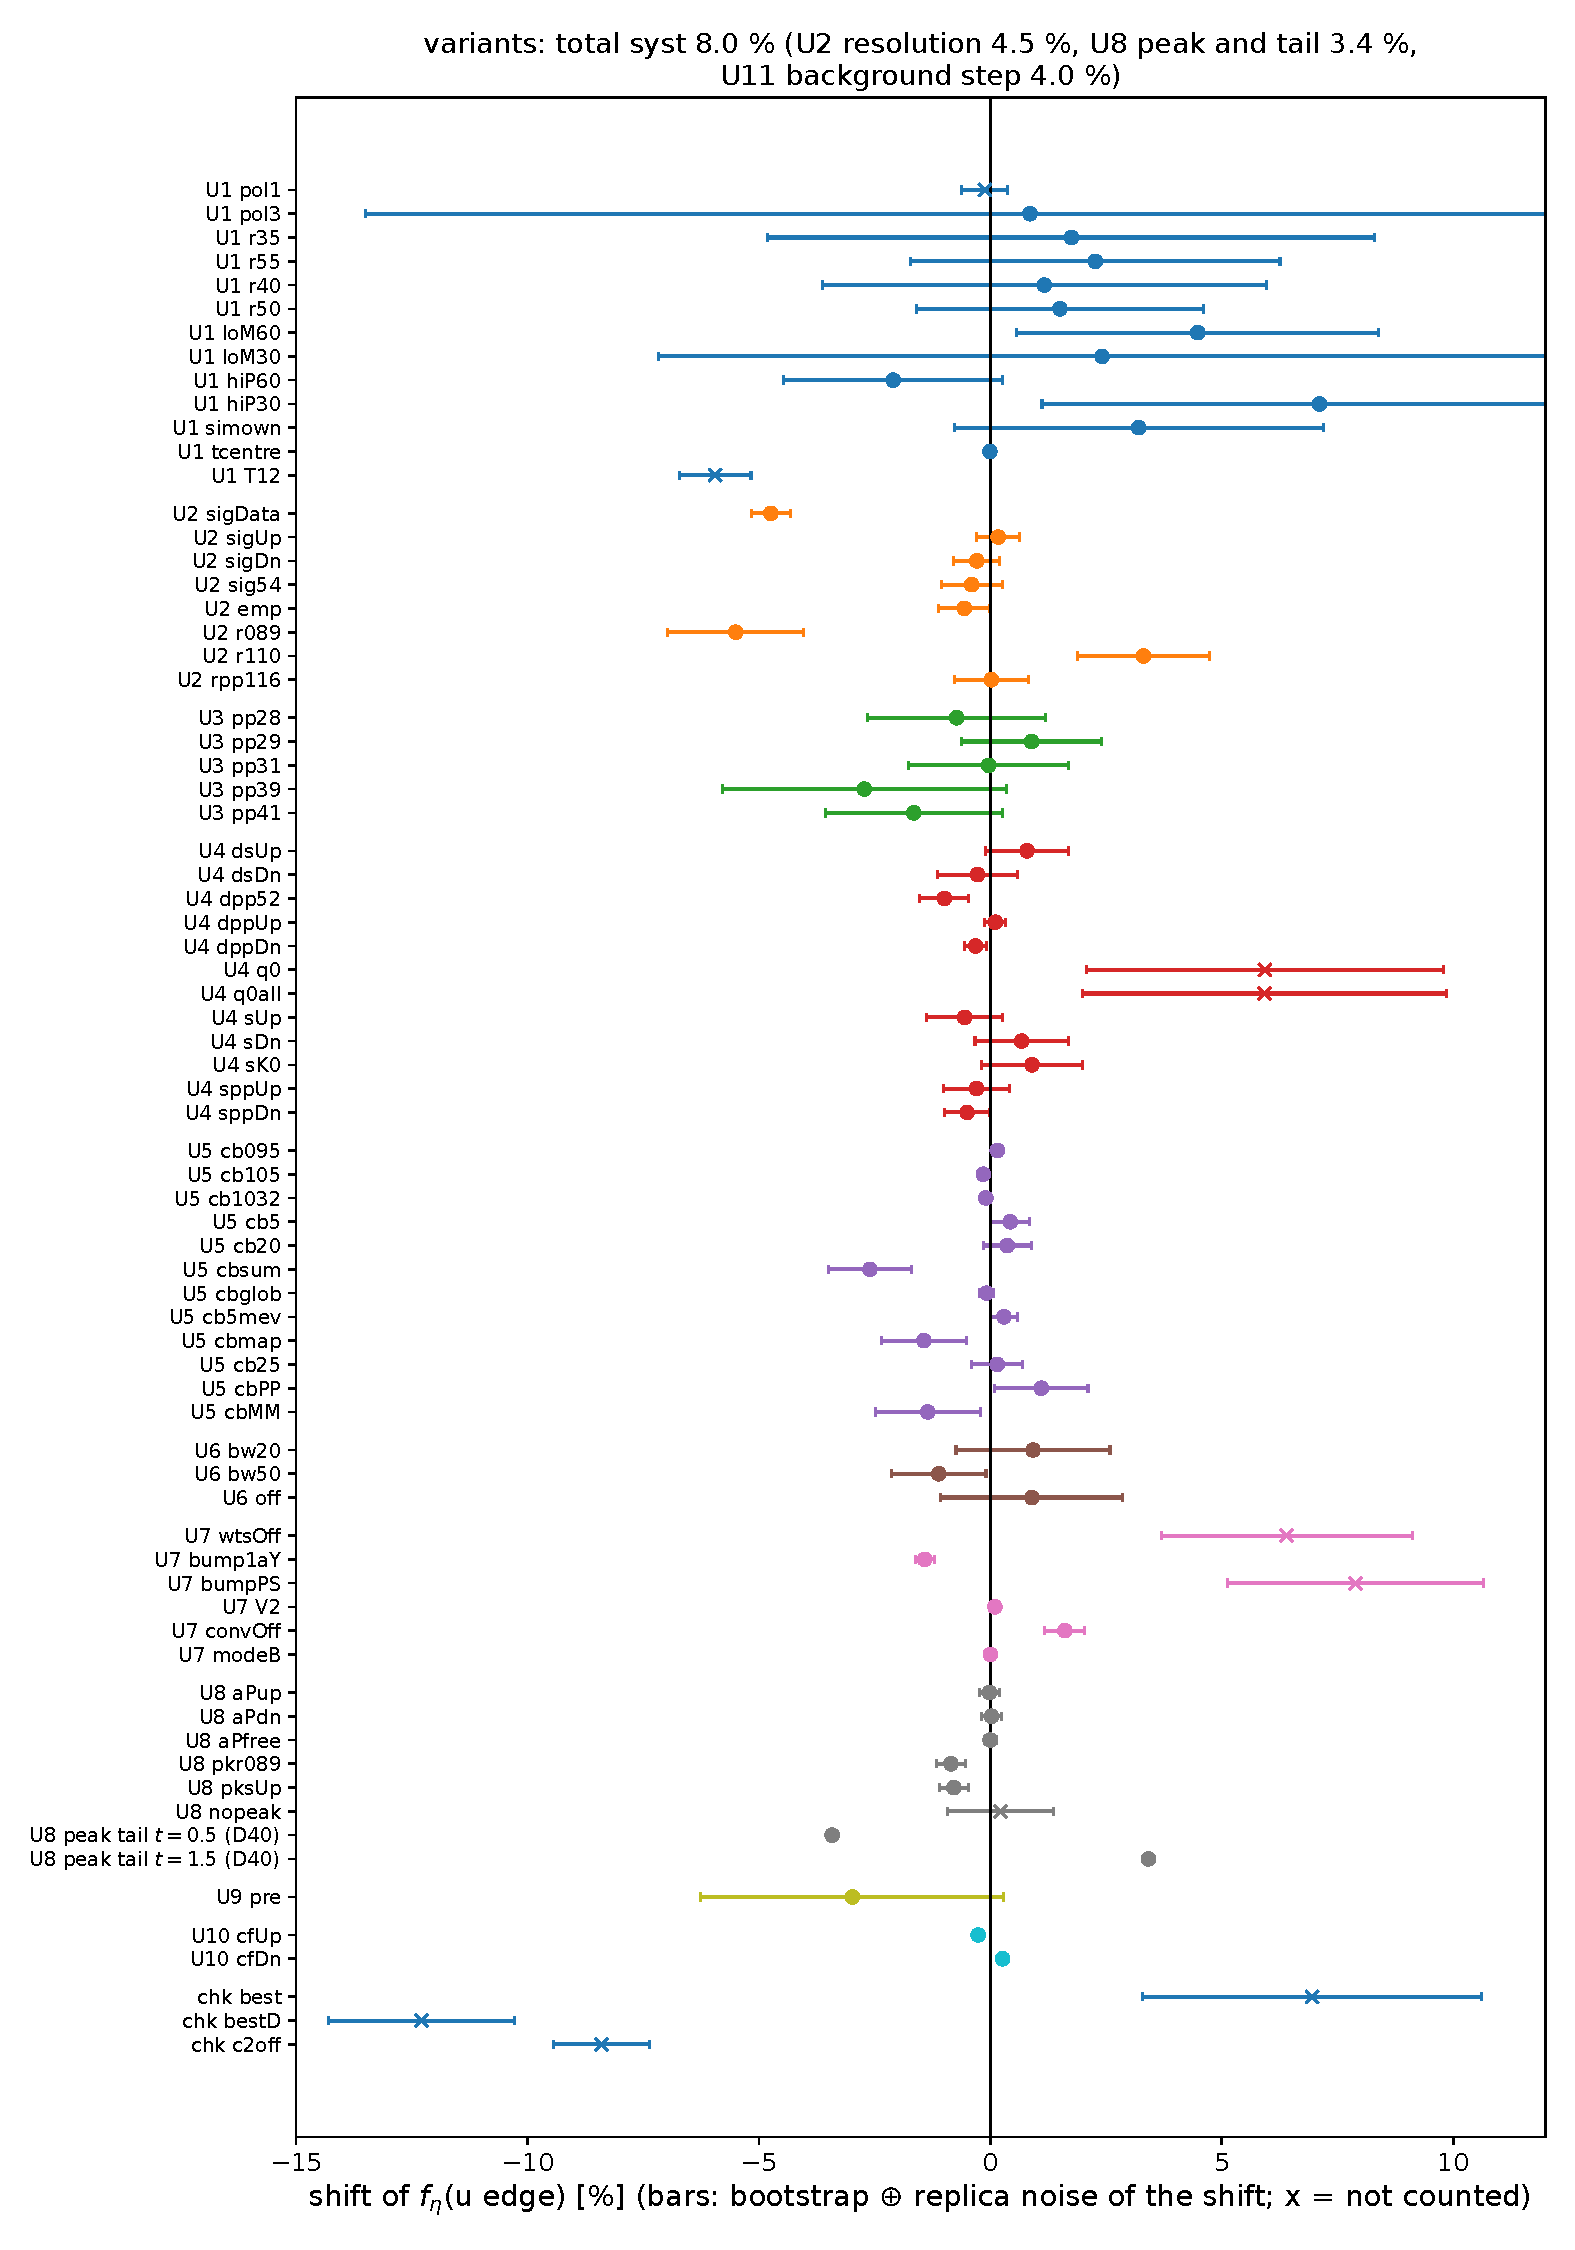
\includegraphics[width=0.60\textwidth]{figs_all/edgeu_syst_v3.pdf}
\caption{\textbf{What it shows: only the resolution variants and the peak tail of D40 (drawn at $t=0.5$ and 1.5) move $f_\eta(u\text{-edge})$ by clearly more than their noise; the excluded
Dalitz-plot variants, $q=0$ and the checks are marked as crosses (not counted).}
Selection: the nominal $u$-edge: data, S0 (PT3 trigger, event vertex in the target region ($\vz>-160$\,mm), \betanew particle identification (pions within $3\sigma$, leptons within $5\sigma$ and with a RICH ring), energy-loss-corrected momenta of all four tracks, all stored combinations of each event (isBest $\ge0$), both pions in the event-vertex fit); $0.30\le\Mpipi<0.40$\,\GeVcc, \Mee$<m_{\piz}=135$\,\MeVcc (where $u$ is defined); $u$ in 2.5\,\MeVcc bins, fit range $-45\le u<45$\,\MeVcc; CB $=2\sqrt{N_{++}N_{--}}$ of the like-sign data in 10\,\MeVcc cells of $u$ per \Mpipi slice (0.30--0.34, 0.34--0.37, 0.37--0.39, 0.39--0.40\,\GeVcc), $k=1$; simulated step from C2 (per-count QED weights) and C3 of SMASH p+p at 4.5\,GeV (standard, lepton and $\eta$ sets, mode A) at its cross sections $\times$ PDG BR $\times$ the $\eta$-decay weights V3, masses moved to the data scale ($M_4'=0.99615\,M_4$, $\Mpipi'=0.9952\,\Mpipi$), same cuts; each variant changes one item (e.g.\ \Mpipi range, $u$ binning, ``pre'' instead of S0).
Shift of every variant in per cent, with the bootstrap $\oplus$ replica noise of the shift; colours: families U1--U10; ``chk'': checks
(isBest $=1$, no C2 factor). U11 (the step that a smooth background projects onto the edge, 4.0\,\%, from the pseudo-data) is \emph{not} shown;
it is in the title and in Table~\ref{tab:edgeu-syst}.}
\label{fig:edgeu-syst}
\end{figure}

\subsection{Consistency tests}
\label{sec:edgeu-cons}
The checks pass except two marginal ones that were also marginal for the per-slice edge (Fig.~\ref{fig:edgeu-checks}): the four slices agree
($\chi^2=1.0/3$), and so do the \Mee classes (E1 0.411, E2 0.444). Periods ($\times\Csec$ per period, simulation $\times L_p/L$): I $0.439\pm0.030$,
IIA $0.396\pm0.084$, IIB $0.538\pm0.046$, III $0.361\pm0.036$, $\chi^2=9.4/3$, $p=0.024$: above the WP7 limit 0.01, so no term is added; it is the
same pattern as per slice (IIB high, III low; $p=0.07$ there). Two random halves of the data: $0.382\pm0.028$ / $0.470\pm0.029$, $z=-2.1$
($p=0.03$), marginal as per slice. ``pre'' (data and simulation) gives 0.413 ($-3.0$\,\%, noise 3\,\%); isBest $=1$ in data and simulation 0.455
(ratio 1.068; per slice 1.085).

\begin{figure}[!htbp]
\centering
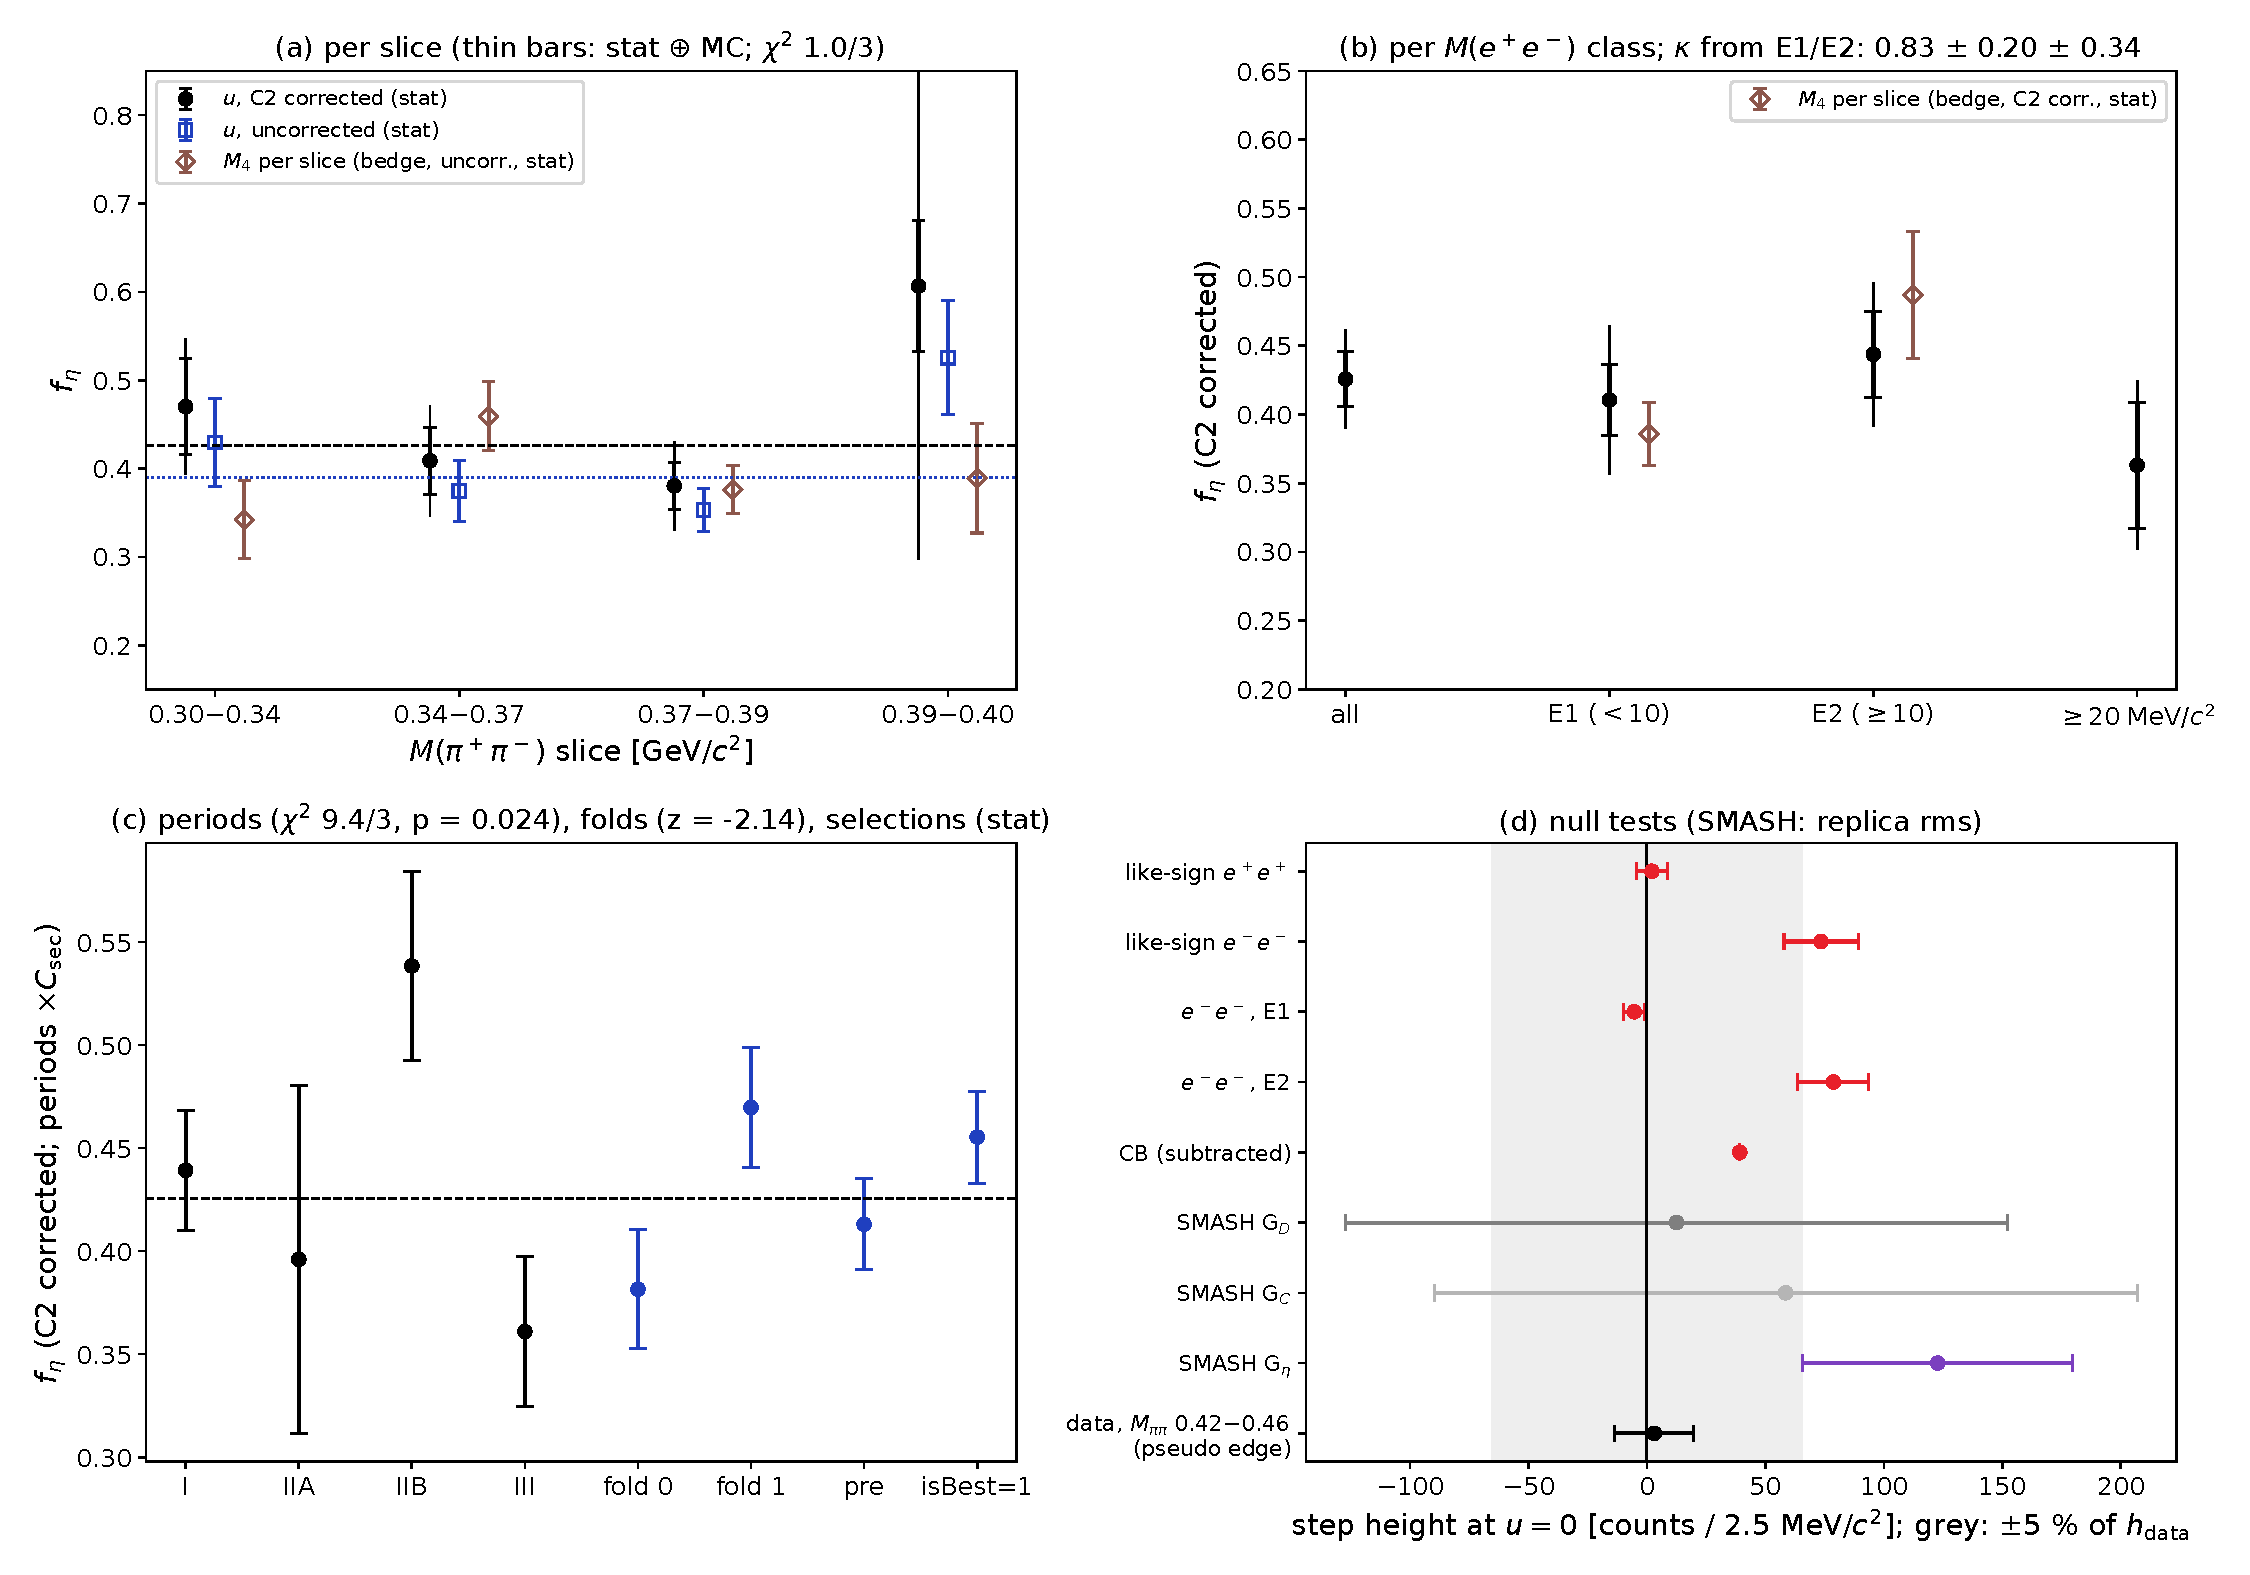
\includegraphics[width=0.92\textwidth]{figs_all/edgeu_checks_v3b.pdf}
\caption{\textbf{What it shows: the slices, the \Mee classes, the periods and the selections agree within their errors (periods and folds
marginal); no sample without a bump has a step at $u=0$, except the $e^-e^-$ like-sign counts (4.7$\sigma$), which contain pairs from the two \piz photons
of the same decays (D39, \S\ref{sec:edgeu-ls}).}
Selection: nominal $u$-edge: data, S0 (PT3 trigger, event vertex in the target region ($\vz>-160$\,mm), \betanew particle identification (pions within $3\sigma$, leptons within $5\sigma$ and with a RICH ring), energy-loss-corrected momenta of all four tracks, all stored combinations of each event (isBest $\ge0$), both pions in the event-vertex fit); $0.30\le\Mpipi<0.40$\,\GeVcc, \Mee$<m_{\piz}=135$\,\MeVcc (where $u$ is defined); $u$ in 2.5\,\MeVcc bins, fit range $-45\le u<45$\,\MeVcc; CB $=2\sqrt{N_{++}N_{--}}$ of the like-sign data in 10\,\MeVcc cells of $u$ per \Mpipi slice (0.30--0.34, 0.34--0.37, 0.37--0.39, 0.39--0.40\,\GeVcc), $k=1$; simulated step from C2 (per-count QED weights) and C3 of SMASH p+p at 4.5\,GeV (standard, lepton and $\eta$ sets, mode A) at its cross sections $\times$ PDG BR $\times$ the $\eta$-decay weights V3, masses moved to the data scale ($M_4'=0.99615\,M_4$, $\Mpipi'=0.9952\,\Mpipi$), same cuts. (a) per \Mpipi slice; (b) \Mee $<10$ and 10--135\,\MeVcc; (c) periods days 034--046, 047--048, 049--053, 059--067 (simulation $\times L_p/L$), the two halves by event-group parity, ``pre'' and isBest $=1$ (only the best-ranked combination) in data and simulation; (d) like-sign counts of S0 (all \Mee and per class), the subtracted CB, SMASH $G_D$, $G_C$, \Geta, and the data at $0.42\le\Mpipi<0.46$\,\GeVcc with a pseudo edge $E(\Mpipi-0.10\,\GeVcc,\Mee)$.
(a) $f_\eta$ per \Mpipi slice: $u$, C2 corrected (black; thick: stat, thin: stat $\oplus$ MC), $u$ uncorrected (blue), the per-slice \Mfour
ratios (brown, data errors only). (b) $f_\eta$ per \Mee class with the per-slice C2-corrected E1/E2 values; $\kappa$ from the E1/E2 split.
(c) Periods ($\times\Csec$), folds, ``pre'', isBest $=1$ (stat). (d) Null tests: step height at $u=0$ of the like-sign counts ($e^+e^+$, $e^-e^-$,
$e^-e^-$ per class), of the subtracted CB, of SMASH $G_D$, $G_C$, \Geta (bars: replica rms; \Geta raw, treated as template noise) and of the data
region \Mpipi 0.42--0.46\,\GeVcc with a pseudo edge; grey: $\pm5$\,\% of $h_{\mathrm{data}}$.}
\label{fig:edgeu-checks}
\end{figure}

\subsection{Pseudo-data}
\label{sec:edgeu-toys}
The truth follows the WP4 recipe in $u$: the data CB per slice; $c\,\times$ the non-$\eta$ background of SMASH (smoothed by exp(pol4) on
$\pm100$\,\MeVcc) $\times(1+bx+qx^2)$, $x=(M_4'-0.55)/0.1$, with optional narrow Gaussian structures in \Mfour and an \Mpipi tilt;
$a\times(\mathrm{C2c}+\kappa\,\mathrm{C3})$ and $a\times$\Geta (smoothed); $a_{Pt}\times(\kappa\,\mathrm{C4}+\mathrm{C5})$. Toys: Poisson $N$ and
like-sign counts, CB rebuilt per slice, the nominal estimator; templates the truth sample (AA) or bootstrap replicas (RF). The estimator closes
within $\pm2$\,\% for smooth backgrounds, with pull widths 0.98--1.07 (AA) and 0.90--1.01 (RF); the coverage of $\pm1\sigma$ is 0.63--0.73
(Table~\ref{tab:edgeu-toys}, Fig.~\ref{fig:edgeu-toys}). The quadratic term $q=-0.173$ that moves B4 by $+150$\,\% moves the $u$-edge by $-2.2$\,\%
(the per-slice edge by $-2.1$\,\%; the verifier, with its own truth and estimator, $-2.0$\,\% Asimov and $-1.9$\,\% in 1000 toys): both edge methods
are about 70 times less sensitive than B4 to this deformation. Both are equally sensitive to a resolution mismatch (the $\eta$ truth at
$r_{\mathrm{res}}=0.89$: $+6.0$\,\% against truth (a)) and to narrow structures (5\,\% at 8\,\MeVcc width: $+7.6$\,\%; 10\,\% at 15\,\MeVcc:
$+17.3$\,\%; per slice $+9$ and $+20$\,\%). The raw SMASH background as truth ($+10$\,\%) is the template noise of the simulated background put into
the truth; it does not enter the estimator, whose simulated step uses the bump classes only, and nothing of this size is seen in the data control
region ($3\pm17$ counts). The Asimov bias is the cleaner number to quote: for truth (a) the AA toy mean lies 0.56\,\% below it, 3.7 times the
standard error of a 1000-toy mean (verifier); no conclusion changes.

\begin{table}[!tbp]
\centering
\caption{\textbf{What it shows: the $u$-edge closes within about 2\,\% for smooth backgrounds; only a resolution mismatch (``mass''), the raw
template noise (``raw'') and narrow structures (``narrow'', ``wide'') bias it.} Pseudo-data, 1000 toys per truth. Truth (a): $c=1.35$, $b=-0.15$,
$a=0.42$; c1: $c=1$, no tilt; a1: $a=1$; q$-$, q$--$, q$+$: quadratic term $-0.173$ (B4 $+150$\,\%), $-0.346$, $+0.173$; om: $\omega/\rho^0$
$\times0.3$, rest $\times1.6$; ty: \Mpipi tilt; sA: stage-A background; sm3/5/6: smoother exp(pol3/5/6); raw: raw SMASH background; mass: $\eta$
truth at $s+0.0009$, $r_{\mathrm{res}}=0.89$; narrow / wide: 5\,\% Gaussian at 0.505 (8\,\MeVcc) / 10\,\% at 0.490\,\GeVcc (15\,\MeVcc) in \Mfour;
kap: $\kappa=0.48$; pk30 / pk55: true peak scale 0.30 / 0.55; datalike: $\kappa=0.48$, $c=1.16$. Source: \code{tables_all/edgeu_toys.txt}.}
\label{tab:edgeu-toys}
\footnotesize
\tabin{edgeu_toys.tex}
\end{table}

\begin{figure}[!htb]
\centering
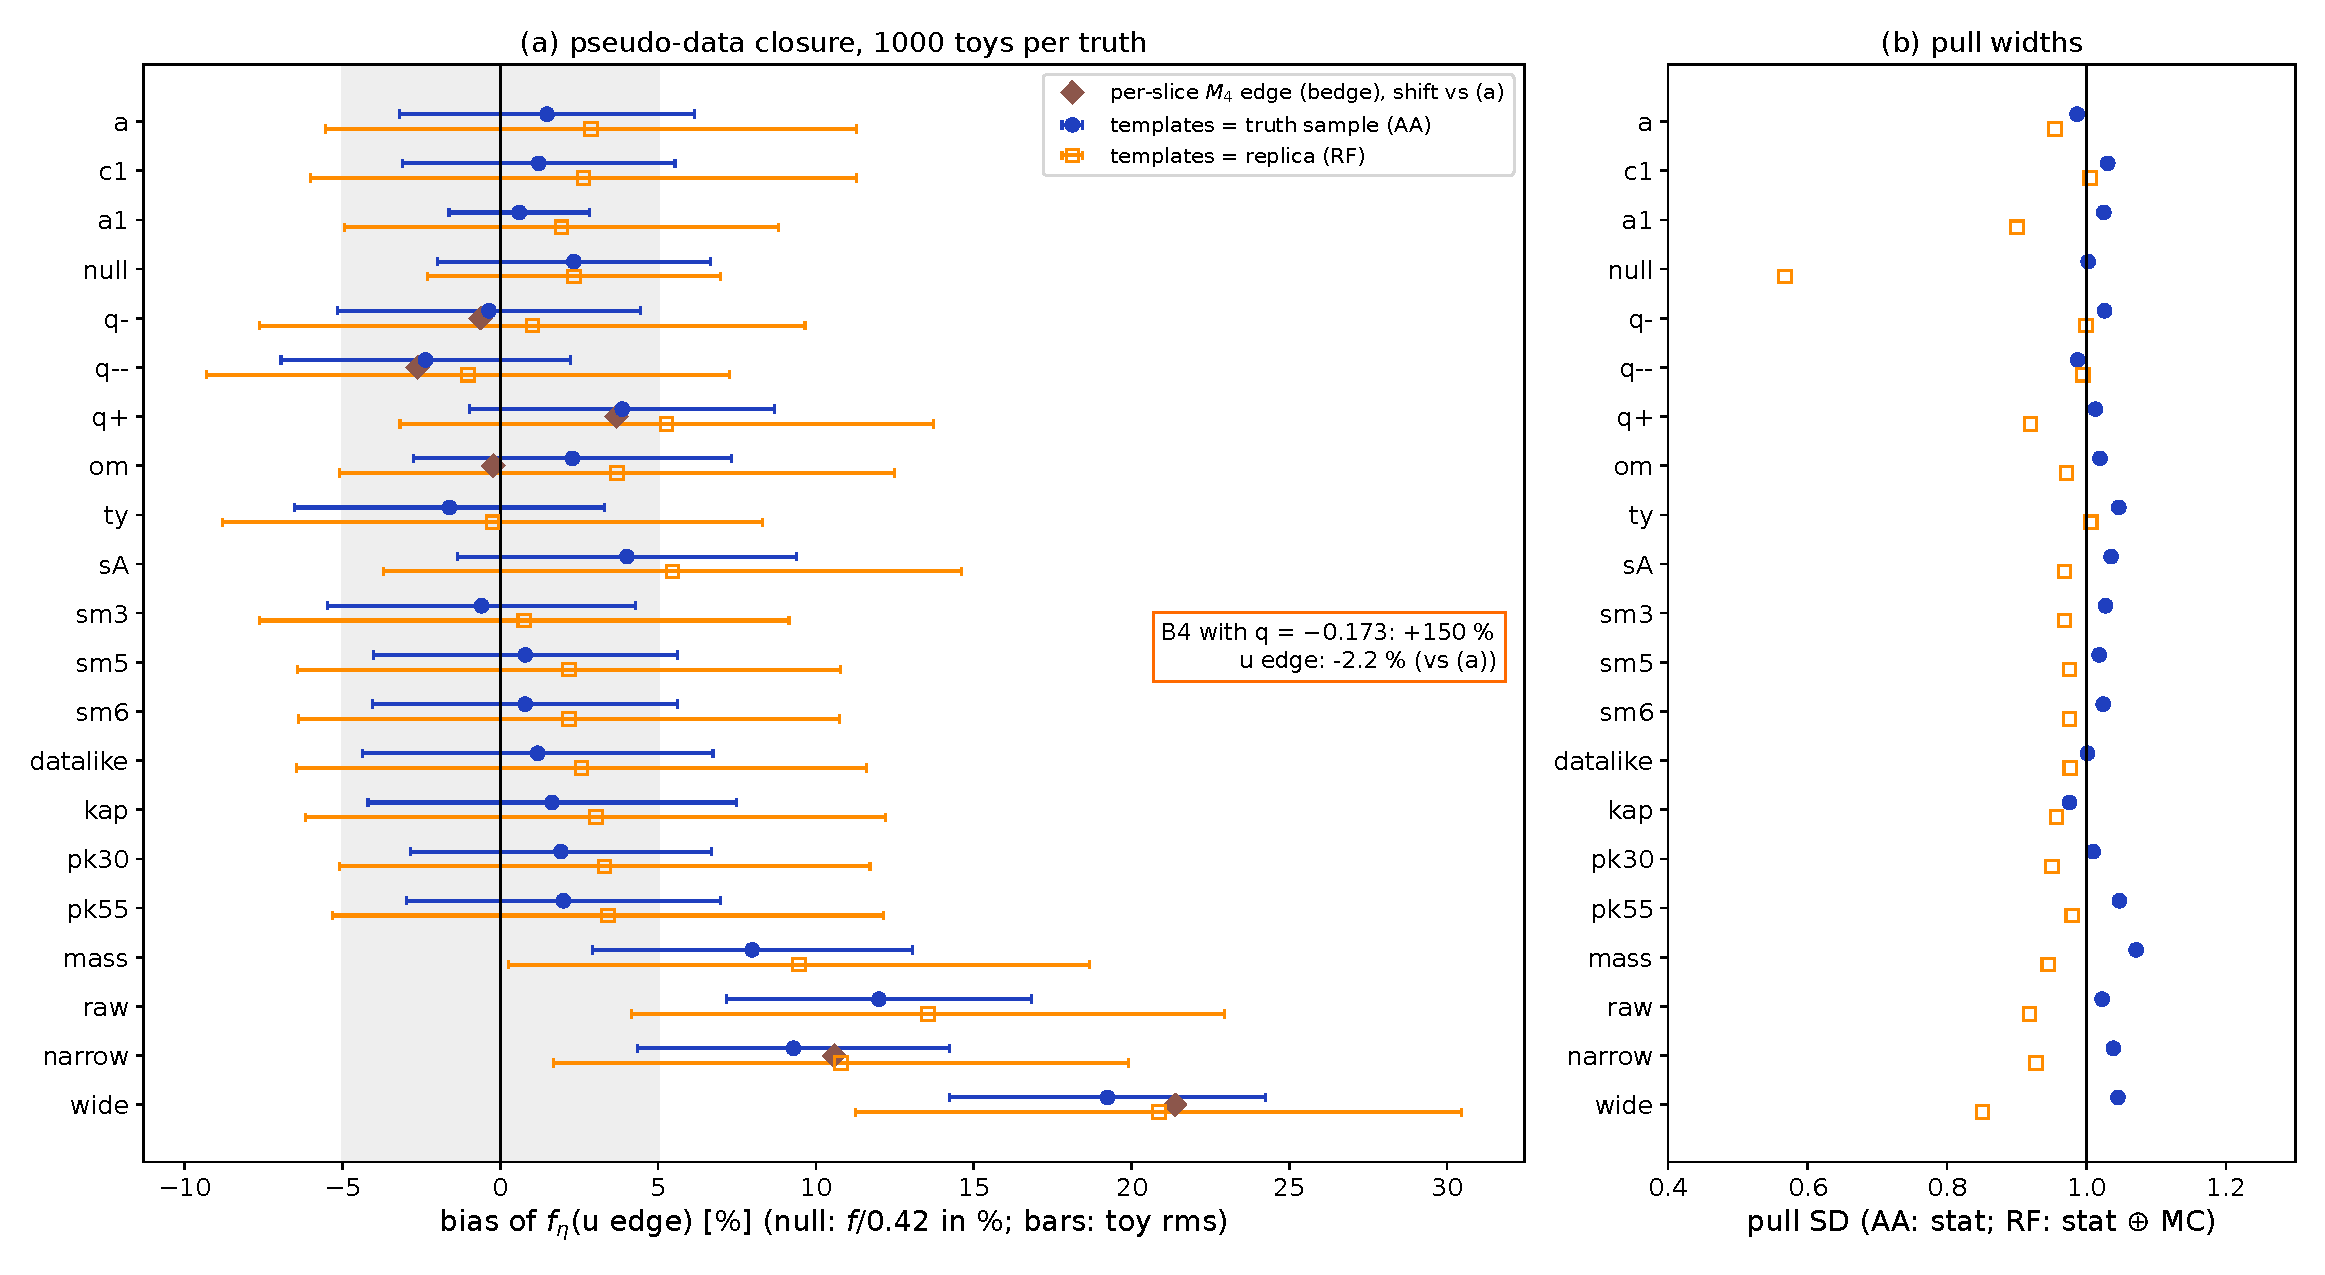
\includegraphics[width=0.86\textwidth]{figs_all/edgeu_toys.pdf}
\caption{\textbf{What it shows: the $u$-edge estimator closes within 2\,\% for smooth backgrounds; the quadratic term that moves B4 by $+150$\,\%
moves it by $-2$\,\%; only a resolution mismatch and background structures as narrow as the edge bias it.}
Selection: pseudo-data only (the measured unlike-sign counts are not used). Each truth is built in the four \Mpipi slices 0.30--0.34, 0.34--0.37, 0.37--0.39 and 0.39--0.40\,\GeVcc, for \Mee below 135\,\MeVcc (where $u$ is defined), from the CB of the data ($2\sqrt{N_{++}N_{--}}$ of the like-sign counts in 10\,\MeVcc cells of $u$ per slice) and from SMASH templates (mode A, $w\times$V3, simulated \Mfour$\times0.99615$ and \Mpipi$\times0.9952$), both with the nominal cuts S0 (PT3 trigger; event vertex in the target region, $\vz>-160$\,mm; START-free \betanew identification, pions within 3$\sigma$, leptons within 5$\sigma$ with a RICH ring; energy-loss-corrected momenta of all four tracks; both pions used in the event-vertex fit; all stored combinations of an event, isBest $\ge0$); every toy is fitted as the data are, in $-45\le u<+45$\,\MeVcc (36 bins of 2.5\,\MeVcc). The brown diamonds use the per-slice \Mfour fit in the same four slices (also S0).
(a) Bias of $f_\eta$ for 21 truths, 1000 toys each: AA (blue), RF (orange squares); brown diamonds: the per-slice \Mfour edge for the same change
of the truth, placed relative to (a); grey band $\pm5$\,\%. (b) Pull widths.}
\label{fig:edgeu-toys}
\end{figure}

\subsection{Yields, \texorpdfstring{\sigeta}{sigma(pp -> eta X)} and the comparison with the per-slice edge}
\label{sec:edgeu-cmp}
\textbf{Yields.} The visible bump yield is $f\times(c\,\mathrm{C2}+\mathrm{C3})_{\mathrm{SMASH}}\times64/63$, with its MC error from the same
replicas: window B, all \Mee, $21\,468\pm1003\pm1708\pm1347$ counts (3.53 visible counts per \nbinv; SMASH $c$C2+C3 $=50\,425.7$ with the
per-count C2 weights); all \Mfour $27\,027\pm1263\pm2150\pm1711$ counts (4.45 visible counts per \nbinv); B in E2 9486 counts (9888 $\pm701\pm926$
with its own E2 fit). \textbf{\sigeta} $=f/1.00436\times1.0694\,\mathrm{mb}\times1.0104\times0.97$ (PDG 2026):
$0.444\pm0.021\pm0.035\pm0.031\,^{+0.043}_{-0.044}$\,mb (C2 corrected with the per-count weights of D38; peak-tail family of D40 included),
0.407\,mb uncorrected, 0.573\,mb with the conversions $\times0.48$ (Table~\ref{tab:edgeu-res}; Fig.~\ref{fig:res-ecompare}). It inherits
the PRELIMINARY label; the one-sided items (live time $+7.3$\,\%, sorter $+1.3$ to $+2.8$\,\%, \code{cor_ok} $+2.2$\,\%, $C_{\mathrm{vtx}}$, the
production model) are not included, as for the peak. \textbf{Double ratio}: $\mathrm{DR}_u=\aP/f_\eta(u\text{-edge})=0.97\pm0.09\,(\mathrm{stat})
\pm0.35\,(\mathrm{syst})\pm0.09\,(\mathrm{MC})$, total $\pm0.37$ (38\,\%; the peak-tail term of D40, $\pm0.05$, listed): the systematic error of
\aP includes the composition term of the peak (35.5\,\%, the \sigeta systematic without the peak tail). The first note quoted $\pm0.22$ with the \aP systematic without that term (16\,\%), as
$\mathrm{DR}_{\mathrm{edge}}$ of \S\ref{sec:bedge-cmp} does (24\,\%); the two conventions must not be compared as like for like. With the
conversions $\times0.48$ in both readings the ratio is about 0.9 (0.88 per slice). Peak and bump are consistent within the 38\,\% uncertainty of the double
ratio: a weak test.

\textbf{Comparison with the per-slice edge.} Both give the same scale (0.426 against 0.423) and the same \sigeta (0.444 against 0.442\,mb). The
total error is 11.6\,\% against 15.4\,\% as quoted for the per-slice edge, but most of this gain comes from taking the simulated step from the bump
classes alone, which the per-slice method can also do (then about 6.6\,\% MC and about 12.4\,\% total with the peak tail, from the replica
decomposition of the per-slice verification; 11.9\,\% before D40). The gain that belongs to $u$ itself is about $12.4\to11.6$\,\%, with a statistical error about 8\,\% smaller (fit errors 4.77\,\% against
5.19\,\%; with $E(m,0)$ in $u$ it is 5.02\,\%, so the \Mee alignment gives about half of it), and the slice choices of the per-slice method
(family E2, 2.9\,\%) disappear. The model dependence is not smaller: both methods rest on the resolution matching at the edge (the data step width,
$7.0\pm0.8$\,\MeVcc, agrees with SMASH, $6.4\pm0.9$) and on the step that a smooth background projects onto the edge; both are tested, not proven.
Four separate fits in $u$ give the same numbers ($0.429\pm0.020\pm0.032$).

\subsection{Data and SMASH compared in \texorpdfstring{$u$}{u}}
\label{sec:edgeu-sim}
\inshort{the analyst asked to \emph{see} the data and SMASH side by side in $u$. Both have the same structure: one step at $u=0$, the $\eta$
peak at $u=+20$ to $+55$\,\MeVcc and a smooth background. SMASH as it is has a bump about 2.3 times too large. With the measured scales it
reproduces the position and the width of the step and the peak region (the size of the step is fitted, so it is not a test), and for
\Mee$\ge10$\,\MeVcc it describes the data ($\chi^2=37.0/36$). For all \Mee the smooth non-$\eta$ background of the model is 1/0.76 too high,
because the stage-A normalisation, fitted for \Mee$\ge10$\,\MeVcc only, is too high at small \Mee (1.6--1.9 standard deviations of its error).
$f_\eta$ is not affected. Independently verified.}

\textbf{What was done} (package udatasim). The data are those of the $u$-edge fit: S0, isBest $\ge0$, $0.30\le\Mpipi<0.40$\,\GeVcc (all \Mpipi
with an edge in Fig.~\ref{fig:edgeu-sim-allmpp}), \Mee$<m_{\piz}$, $N-\mathrm{CB}$ in counts per 2.5\,\MeVcc, with CB $=2\sqrt{N_{++}N_{--}}$ of
the data per \Mpipi slice in 10\,\MeVcc cells of $u$ ($k=1$, as in the fit; the simulation never provides the CB). SMASH is stacked class by
class (C2, C3, C4, C5, \Geta, $G_D$, $G_C$) in expected counts ($\sum w\times6079.2/221.05\times63/64$, mode A, $w\times$V3,
$M_4'=0.99615\,M_4$, $\Mpipi'=0.9952\,\Mpipi$, D8) in two versions: (a) SMASH as it is, $\sigma_{\mathrm{prod}}\times$PDG BR, no scale; (b)
SMASH with the measured scales of Table~\ref{tab:edgeu-sim-scales}. All scales of (b) come from elsewhere in this report; nothing is fitted to
these figures. The nominal $u$-edge fit was first rebuilt with the frozen code (to the last digit); with the per-count C2 weights of D38 it gives
$f_\eta(u)=0.42574$, the value used. Errors: data $N$ from event groups (variance 1.0017 times the count), the CB from its like-sign counts,
the simulation MC from the simulated event groups; the stage-A normalisation error is propagated from its covariance and drawn as a band.
$\chi^2$ is given with the statistical errors, with the stage-A covariance added (``$+$A''), and with one free factor $\lambda$ on $G_D+G_C$
(one degree of freedom less; not the $\lambda$ of the flexible fit). $f_\eta$ was fitted on the same bins of $-45\le u<+45$\,\MeVcc (with a pol2
background, not with this model), so 35 would be the strict number of degrees of freedom there.

\begin{table}[!tbp]
\centering
\caption{\textbf{What it shows: the scales of model (b) and where each comes from.} Nothing is fitted to the data/SMASH figures of
\S\ref{sec:edgeu-sim}. $x=(M_4'-0.55)/0.1$; the slice $j$ of a simulated count is taken from $\Mpipi'$ ($c_5=0.909$ is not used: $u$ exists only
below \Mpipi$=0.4116$\,\GeVcc). Stage A: Poisson maximum likelihood, model M1, \Mee$\ge10$\,\MeVcc (E2), CR-U 0.575--0.700\,\GeVcc
(\code{stageA.txt}); its total errors are dominated by the simulation statistics ($c_j\pm0.20$, $\kB\pm1.45$, 97--98\,\% correlated).}
\label{tab:edgeu-sim-scales}
\small
\begin{tabularx}{\textwidth}{@{}>{\raggedright\arraybackslash}p{5.0cm} >{\raggedright\arraybackslash}p{4.9cm} L@{}}
\toprule
class & scale in (b) & source \\
\midrule
C2 (bump: \piz Dalitz, photon lost) & per-count QED weight (D38; mean 0.864) $\times f_\eta(u)=0.426$ & the $u$-edge fit with the D38 weights
(\S\ref{sec:edgeu-fit}, \S\ref{sec:c2recon}) \\
C3 (bump: one \piz photon converted, the other lost) & $\times f_\eta(u)=0.426$ & as C2 \\
C4 (peak: $\eta\to\pipi\gamma$, $\gamma$ converted) & $\times\aP=0.418$ & peak side bands (\S\ref{sec:sb}) \\
C5 (peak: direct $\eta\to\ppee$) & $\times\aP=0.418$ & as C4 \\
\Geta (other $\eta$ decays) & $\times\aEta g=0.656$ & effective \Geta scale of the peak side bands (F-main $\aEta=0.382$, $g=1.717$;
\S\ref{sec:fmain}, \S\ref{sec:b4}) \\
$G_D$ (non-$\eta$ Dalitz and vector-meson pairs) & $\times c_j(1+bx)$; $c_{1\ldots4}=0.988$, 1.001, 0.975, 1.055; $b=-0.068$ & stage A
(Fig.~\ref{fig:res-after}, Table~\ref{tab:C2}) \\
$G_C$ (non-$\eta$ conversion pairs) & $\times c_j(1+bx)\,\kB$, $\kB=3.06\pm1.45$ & as $G_D$ \\
\bottomrule
\end{tabularx}
\end{table}

\textbf{What the figures show} (Figs.~\ref{fig:edgeu-sim}--\ref{fig:edgeu-sim-mee}, Table~\ref{tab:edgeu-sim}).
\begin{itemize}\setlength{\itemsep}{1pt}
\item \textbf{The same structure.} One step at $u=0$ (the bump), the $\eta$ peak at $u=+20$ to $+55$\,\MeVcc, a smooth background that rises with
      $u$. No SMASH class other than the bump has a step at $u=0$ (as the null tests of \S\ref{sec:edgeu-spec} found).
\item \textbf{SMASH as it is (a) does not describe the data:} data/model 0.82 below the edge and 1.15 above, $\chi^2=178/36$ and 106/16; its bump
      is about 2.3 times too large ($1/f_\eta$), and above the peak its background is too low, as in Fig.~\ref{fig:res-before}.
\item \textbf{With the measured scales (b) the step and the peak region fit.} The ratio is flat across the edge (0.765 / 0.783 / 0.765 for all
      \Mee). The position and the width of the step are a test; its size is not, because $f_\eta$ was fitted on these bins.
\item \textbf{Where stage A was fitted (\Mee$\ge10$\,\MeVcc, E2), model (b) describes the data:} $\chi^2=37.0/36$ and 11.1/16, data/model
      0.95 / 0.92 / 0.95 (Fig.~\ref{fig:edgeu-sim-mee}, right).
\item \textbf{The only mismatch beyond the statistical errors is the level of the smooth non-$\eta$ background:} for all \Mee the model is
      1/0.76 too high at every $u$, for \Mee$<10$\,\MeVcc (E1) 1/0.65. One free factor on $G_D+G_C$ removes it: $\lambda=0.730\pm0.022$,
      $\chi^2=32.9/35$ and 6.1/15, data/model 0.96--1.02; in E2 alone $\lambda=0.955\pm0.030$ (consistent with 1), in E1 0.61.
\item \textbf{For all \Mpipi with an edge the picture is the same} (Fig.~\ref{fig:edgeu-sim-allmpp}).
\end{itemize}

\textbf{Why the level is off at small \Mee.} Stage A dropped E1 (fall-back, \S\ref{sec:step0}) and was fitted in E2, where $G_D$ and $G_C$ have
similar shapes and only their sum is fixed (correlation of $c_j$ and \kB $-0.92$); its $\kB=3.06$ is therefore loosely defined ($\pm1.45$).
Carried to E1, where the conversion pairs dominate, it makes $G_C$ much larger: below the edge $G_C$ goes from 8886 counts (SMASH as it is) to
28\,198 ($\times3.17$), as large as the whole data $N-\mathrm{CB}$ there (28\,074); in E2 $G_C$ is 6918 of 23\,774. SMASH as it is treats E1 no
worse than E2 (data/(a) 0.81 / 0.99 / 1.19 in E1, 0.83 / 0.90 / 1.10 in E2). With the other scales of (b) held fixed, the E1 data want a
conversion factor of 1.46 below the edge, 1.71 at it and 1.69 above, instead of 3.06: about one standard deviation of \kB taken alone. F-main
showed the same: its E1 data are 0.75--0.90 of the prediction from the E2 parameters (\S\ref{sec:fmain}). Statistically the difference is large
($\lambda=0.730\pm0.022$). With every error, the stage-A normalisation included, data minus model is $-1.84$ / $-1.61$ / $-1.60$ standard
deviations in the three bands for all \Mee (E1 $-1.87$ / $-1.53$ / $-1.65$; E2 $-0.67$ / $-0.85$ / $-0.58$), in line with the ``$+$A'' $\chi^2$
of 18.9/36. $f_\eta$ is not affected: the edge fit takes its smooth part from the data (pol2), not from SMASH.

\begin{table}[!t]
\centering
\caption{\textbf{What it shows: SMASH as it is (a) describes no sample; with the measured scales (b) only the level of the non-$\eta$ background
is off, one free factor $\lambda$ on it removes the mismatch, and for \Mee$\ge10$\,\MeVcc model (b) describes the data as it is.} Data S0, isBest
$\ge0$. Top: $\chi^2$ with statistical errors (data, CB and simulation MC; number of bins in brackets); ``$+$A'' adds the stage-A
normalisation covariance (not a strong test: that covariance is dominated by template noise and lets normalisation, tilt and the $G_C$/$G_D$
mix move far); $\lambda\to\chi^2$: one free factor on $G_D+G_C$ fitted in that range (one degree of freedom less). Bottom: data/model in
three bands of $u$, with the statistical error and, for (b), second, the stage-A normalisation error; ``(b), $\lambda$'': (b) with the free factor ($\lambda=0.730$; all \Mpipi 0.725). E1: \Mee$<10$, E2: \Mee$\ge10$\,\MeVcc; all
\Mpipi: $0.27\le\Mpipi<0.415$\,\GeVcc (the edge exists below 0.4116). Source: \code{udatasim_overlay.json}, reproduced by the verifier
(\code{udatasim_verify.json}).}
\label{tab:edgeu-sim}
\footnotesize
\setlength{\tabcolsep}{4pt}
\begin{tabular*}{\textwidth}{@{\extracolsep{\fill}}l c r r l r r l@{}}
\toprule
 & & \multicolumn{3}{c}{$-45\le u<+45$\,\MeVcc (36)} & \multicolumn{3}{c}{$+20\le u<+60$\,\MeVcc (16)} \\
\cmidrule(lr){3-5}\cmidrule(l){6-8}
sample & model & stat & $+$A & $\lambda\to\chi^2$ & stat & $+$A & $\lambda\to\chi^2$ \\
\midrule
0.30--0.40, all \Mee & (a) & 177.6 & -- & $1.057\to170.8$ & 105.8 & -- & $1.221\to18.0$ \\
                     & (b) & 187.3 & 18.9 & $0.730\pm0.022\to32.9$ & 97.4 & 5.7 & $0.736\to6.1$ \\
0.30--0.40, E1       & (b) & 203.1 & 19.6 & $0.609\pm0.029\to24.9$ & 108.2 & 6.0 & $0.619\to4.9$ \\
0.30--0.40, E2       & (a) & 83.8 & -- & $1.027\to82.9$ & 50.3 & -- & $1.187\to12.2$ \\
                     & (b) & \textbf{37.0} & 23.3 & $0.955\pm0.030\to34.9$ & \textbf{11.1} & 6.4 & $0.945\to9.0$ \\
all \Mpipi, all \Mee & (a) & 198.8 & -- & $1.077\to183.2$ & 148.9 & -- & $1.245\to18.3$ \\
                     & (b) & 226.6 & 19.0 & $0.725\pm0.020\to32.9$ & 104.6 & 5.9 & $0.750\to6.5$ \\
all \Mpipi, E1       & (b) & 245.1 & 19.0 & $0.604\to23.9$ & 117.5 & 6.3 & $0.636\to5.8$ \\
all \Mpipi, E2       & (b) & \textbf{39.6} & 26.2 & $0.950\to36.3$ & \textbf{11.6} & 7.6 & $0.948\to9.4$ \\
\bottomrule
\end{tabular*}

\vspace{0.6em}
\setlength{\tabcolsep}{3pt}
\begin{tabular*}{\textwidth}{@{\extracolsep{\fill}}l l l l l@{}}
\toprule
 & & \multicolumn{3}{c}{data/model in three bands of $u$ [\MeVcc]} \\
\cmidrule(l){3-5}
sample & model & $-45\ldots-5$ & $-5\ldots+5$ & $+5\ldots+45$ \\
\midrule
0.30--0.40, all \Mee & (a) & $0.820\pm0.017$ & $0.941\pm0.038$ & $1.146\pm0.021$ \\
                     & (b) & $0.765\pm0.022\pm0.095$ & $0.783\pm0.042\pm0.097$ & $0.765\pm0.020\pm0.111$ \\
                     & (b), $\lambda$ & $0.964\pm0.034$ & $1.008\pm0.069$ & $1.015\pm0.036$ \\
0.30--0.40, E1       & (b) & $0.655\pm0.026\pm0.118$ & $0.694\pm0.053\pm0.129$ & $0.652\pm0.024\pm0.136$ \\
0.30--0.40, E2       & (b) & $\mathbf{0.953\pm0.036\pm0.056}$ & $\mathbf{0.919\pm0.065\pm0.059}$ & $\mathbf{0.954\pm0.034\pm0.067}$ \\
all \Mpipi, all \Mee & (a) & $0.839\pm0.016$ & $0.943\pm0.035$ & $1.164\pm0.020$ \\
                     & (b) & $0.753\pm0.020\pm0.098$ & $0.761\pm0.038\pm0.096$ & $0.765\pm0.019\pm0.111$ \\
                     & (b), $\lambda$ & $0.960\pm0.032$ & $0.991\pm0.063$ & $1.023\pm0.033$ \\
all \Mpipi, E2       & (b) & $0.953\pm0.033\pm0.058$ & $0.890\pm0.058\pm0.059$ & $0.954\pm0.031\pm0.067$ \\
\bottomrule
\end{tabular*}
\end{table}

\begin{figure}[!tbp]
\centering
\captionsetup{singlelinecheck=false}% long caption: skip the one-line test (its trial box would exceed TeX's largest dimension)
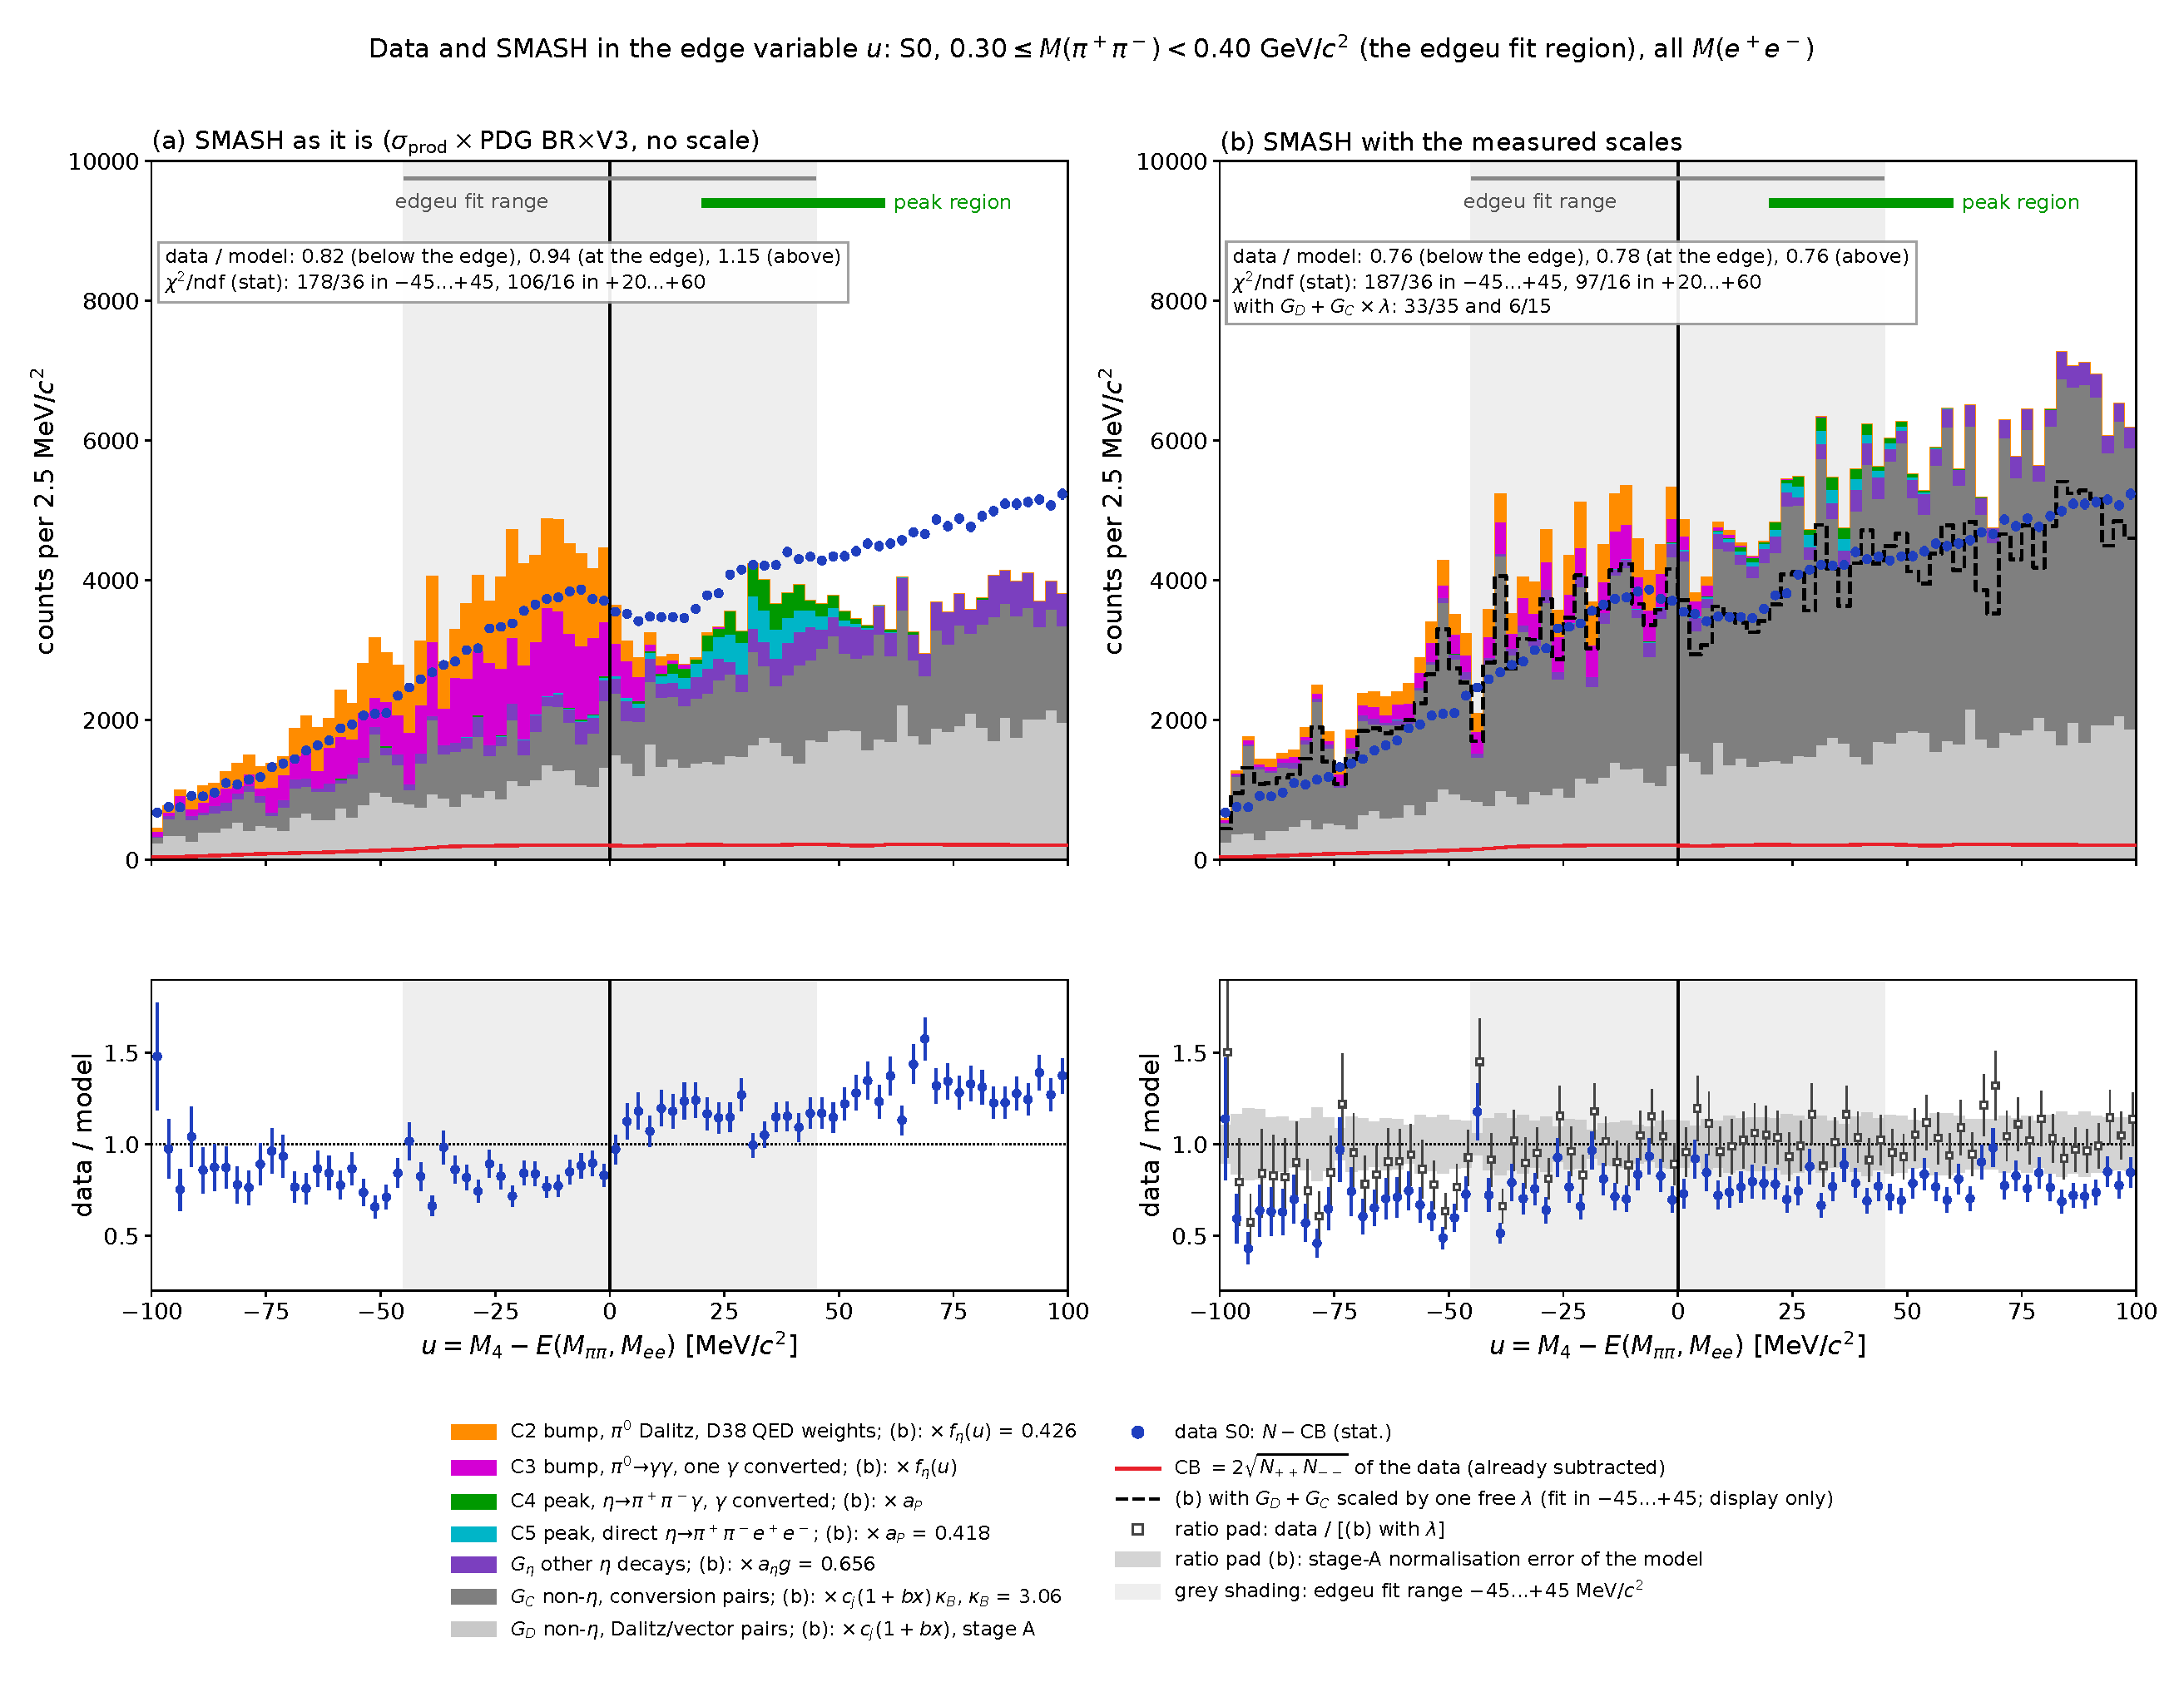
\includegraphics[width=0.68\textwidth]{figs_all/udatasim_u_overlay.pdf}
\caption{\textbf{What it shows: in the variable $u$ the data and SMASH have the same structure: one step at $u=0$ from the bump, the $\eta$ peak
at $u=+20$ to $+55$\,\MeVcc, and a smooth background that rises with $u$. With the measured $\eta$ scales (b), SMASH reproduces the position and
the width of the data step and the shape of the peak region; the step size is fixed by $f_\eta(u)$, which was fitted to these data. The one
difference beyond the statistical errors is the level of the smooth non-$\eta$ background. The normalisation of Fig.~\ref{fig:res-after} was
fitted for \Mee$\ge10$\,\MeVcc; carried to all \Mee, it puts the model 1/0.76 too high at every $u$ (1/0.65 below 10\,\MeVcc, 1/0.95 above,
within errors). This is 1.6--1.9 standard deviations of the stage-A normalisation error (grey band).}
Selection: data and SMASH (mode A, $w\times$V3, \Mfour$\times0.99615$, \Mpipi$\times0.9952$) with the nominal cuts S0 (PT3 trigger; event vertex in the target region, $\vz>-160$\,mm; START-free \betanew identification, pions within 3$\sigma$, leptons within 5$\sigma$ with a RICH ring; energy-loss-corrected momenta of all four tracks; both pions used in the event-vertex fit; all stored combinations of an event, isBest $\ge0$); $0.30\le\Mpipi<0.40$\,\GeVcc; \Mee below 135\,\MeVcc.
Data S0 (isBest $\ge0$), $0.30\le\Mpipi<0.40$\,\GeVcc, all \Mee (below $m_{\piz}$, where $u$ is defined), $L=6079.2\,\nbinv$: $N-\mathrm{CB}$
per 2.5\,\MeVcc (blue) in counts (stored \ppee combinations). CB $=2\sqrt{N_{++}N_{--}}$ from the like-sign data (red line, already subtracted),
per \Mpipi slice in 10\,\MeVcc cells of $u$. Stack: SMASH in expected counts (as described in the text); C2 carries the per-count QED
weights of D38. C2 orange, C3 magenta, C4 green, C5 cyan, \Geta
violet, $G_C$ dark grey, $G_D$ light grey, as in Fig.~\ref{fig:res-after} (the $u$ spectra of Fig.~\ref{fig:edgeu-spec} use the reverse
greys). Lepton pairs from the two different photons of a \piz (cross-photon pairs) are produced by SMASH but are not part of these SMASH
templates: they are left to the CB taken from the data. (a) SMASH as it is ($\sigma_{\mathrm{prod}}\times$PDG BR). (b) The measured scales (Table~\ref{tab:edgeu-sim-scales}): C2 and C3
$\times f_\eta(u)=0.426$ (the $u$-edge fit with the D38 weights); C4 and C5 $\times\aP=0.418$; \Geta$\times\aEta g=0.656$; $G_D$ and $G_C$
$\times$ the stage-A normalisation of Fig.~\ref{fig:res-after} ($c_j(1+bx)$, $\kB=3.06$ on $G_C$); dashed: (b) with $G_D+G_C$ scaled by one
free factor $\lambda=0.73$, fitted in $-45\ldots+45$\,\MeVcc (display only). Lower pads: data/model with statistical errors (data and
simulation MC combined); in (b) grey band: the stage-A normalisation error; open squares: data/[(b) with $\lambda$]. Light grey shading: the
$u$-edge fit range $-45\ldots+45$\,\MeVcc; black line: $u=0$; green bar: the peak region $+20\ldots+60$\,\MeVcc. Panel text: data/model in
three bands of $u$ and $\chi^2$ (statistical), as in Table~\ref{tab:edgeu-sim}. What not to over-read (the full list closes this section):
the level of (b) is the stage-A normalisation, fitted for \Mee$\ge10$\,\MeVcc and carried here to \Mee$<10$\,\MeVcc, where $\kB=3.06$ makes
the conversion background too high (data/model 0.65 there, 0.95 for \Mee$\ge10$\,\MeVcc, Fig.~\ref{fig:edgeu-sim-mee}); statistically large
($\lambda=0.73\pm0.02$), this is 1.6--1.9 standard deviations of the stage-A normalisation error (grey band), which is dominated by the MC
error of \kB ($3.06\pm1.45$), and it does not enter $f_\eta$ (the $u$-edge fit takes its smooth part from the data). The step height in (b)
is not a test ($f_\eta$ was fitted on these data). A simulated conversion-background ($G_C$) count stands for about 27 expected counts,
$\times3.06$ in (b), so about 84; the spikes of the stack are this template. \Geta ($\times0.656$, not a robust scale) is 3.5\,\% of the model
(5\,\% for \Mee$\ge10$\,\MeVcc). Package udatasim, independently verified.}
\label{fig:edgeu-sim}
\end{figure}

\begin{figure}[!tbp]
\centering
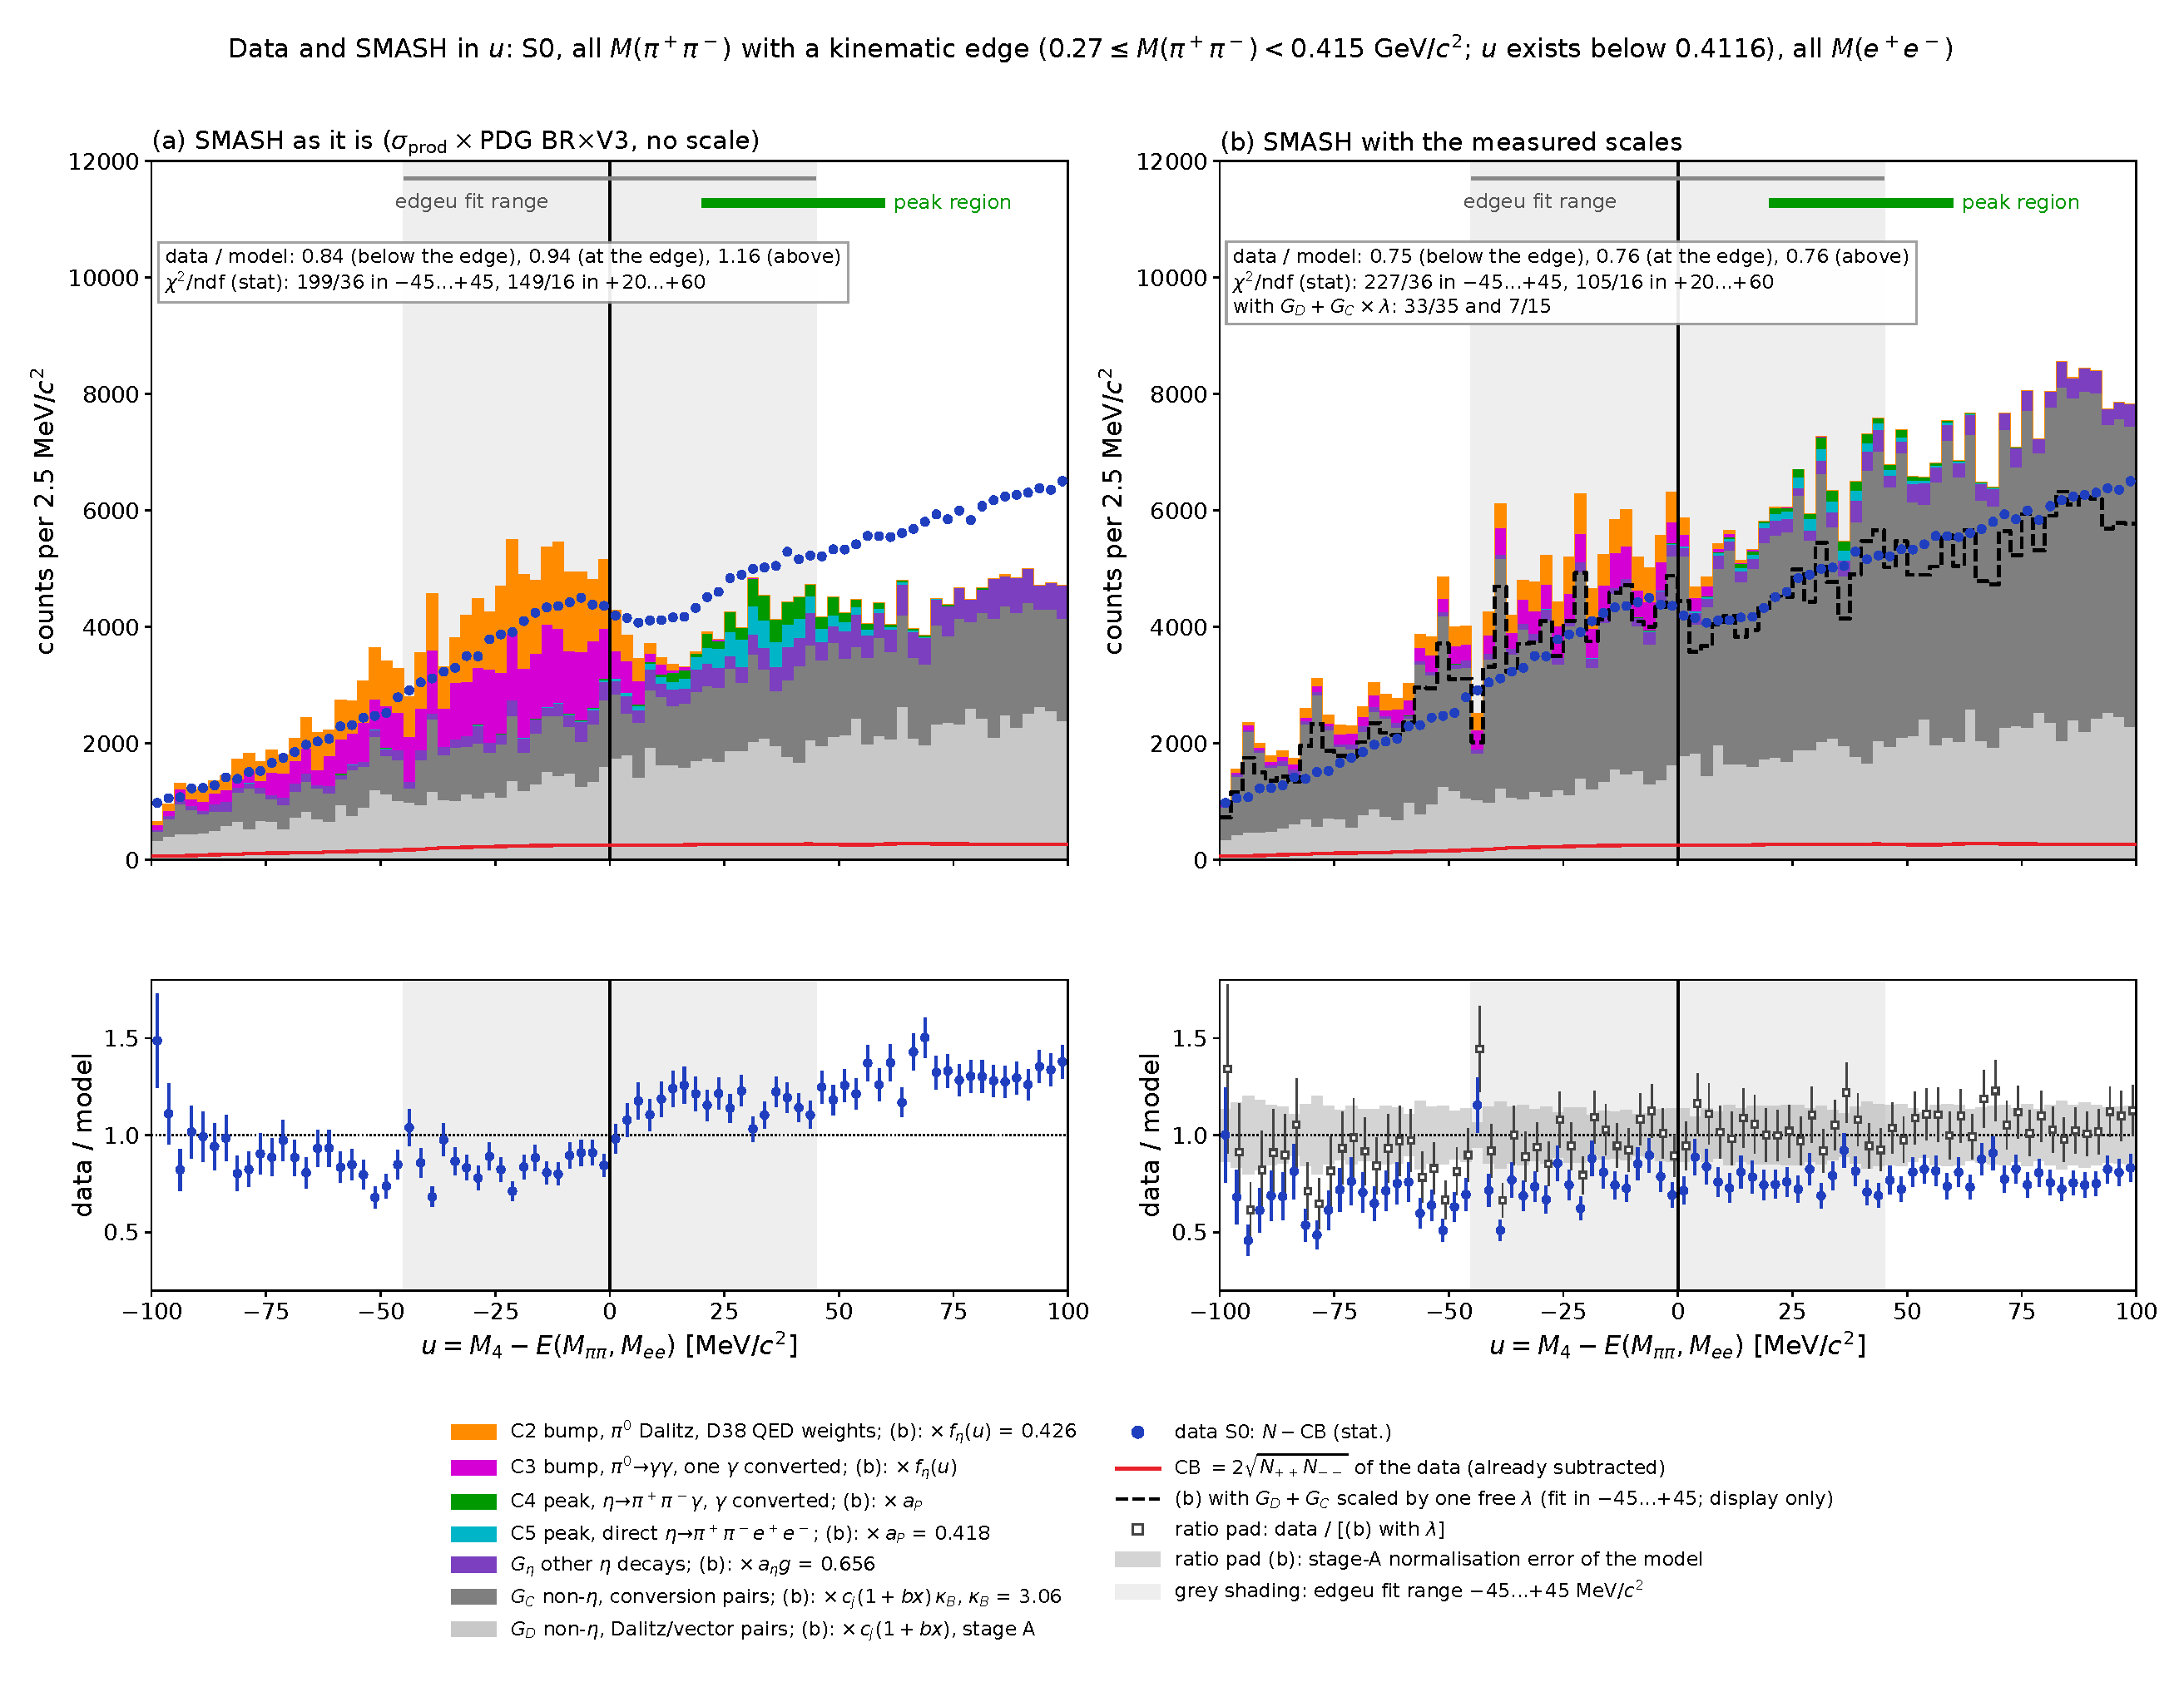
\includegraphics[width=\textwidth]{figs_all/udatasim_u_overlay_allmpp_v2.pdf}
\caption{\textbf{What it shows: the same comparison for all \Mpipi where the bump has an edge. The picture does not change: one step at $u=0$,
whose position and width SMASH with the measured scales reproduces, and a smooth background whose level in (b) is 1/0.76 too high, from the
small-\Mee pairs.}
Selection: as Fig.~\ref{fig:edgeu-sim}, data at $L=6079.2\,\nbinv$ with the nominal cuts S0 (PT3 trigger; event vertex in the target region, $\vz>-160$\,mm; START-free \betanew identification, pions within 3$\sigma$, leptons within 5$\sigma$ with a RICH ring; energy-loss-corrected momenta of all four tracks; both pions used in the event-vertex fit; all stored combinations of an event, isBest $\ge0$), all \Mee below 135\,\MeVcc (where $u$ is defined), SMASH with the same cuts (mode A, $w\times$V3, simulated \Mfour$\times0.99615$ and \Mpipi$\times0.9952$), but for $0.27\le\Mpipi<0.415$\,\GeVcc, with the CB ($2\sqrt{N_{++}N_{--}}$ of the like-sign data, 10\,\MeVcc cells of $u$, $k=1$) computed separately in the slices 0.27--0.30, 0.30--0.34, 0.34--0.37, 0.37--0.39, 0.39--0.40 and 0.40--0.415\,\GeVcc.
As Fig.~\ref{fig:edgeu-sim}, for $0.27\le\Mpipi<0.415$\,\GeVcc: the edge exists only below 0.4116\,\GeVcc, and 0.27--0.28\,\GeVcc holds 0.1\,\%
of the counts; the title gives the selection, 0.27--0.415\,\GeVcc. The CB is computed per slice (0.27--0.30, 0.30--0.34, 0.34--0.37, 0.37--0.39, 0.39--0.40 and
0.40--0.415\,\GeVcc). The scales are the same; $f_\eta$ and the fit range belong to the 0.30--0.40\,\GeVcc fit. (a): data/model 0.84 / 0.94 /
1.16, $\chi^2=199/36$ and 149/16; (b): 0.75 / 0.76 / 0.76, $\chi^2=227/36$ and 105/16; with $\lambda=0.725$: 0.96 / 0.99 / 1.02,
$\chi^2=33/35$ and 6.5/15. Outside 0.30--0.40\,\GeVcc the peak lies at $u=+24$ (\Mpipi$=0.28$\,\GeVcc) to about $+65$\,\MeVcc (0.41\,\GeVcc),
so the peak region is broader.}
\label{fig:edgeu-sim-allmpp}
\end{figure}

\begin{figure}[!tbp]
\centering
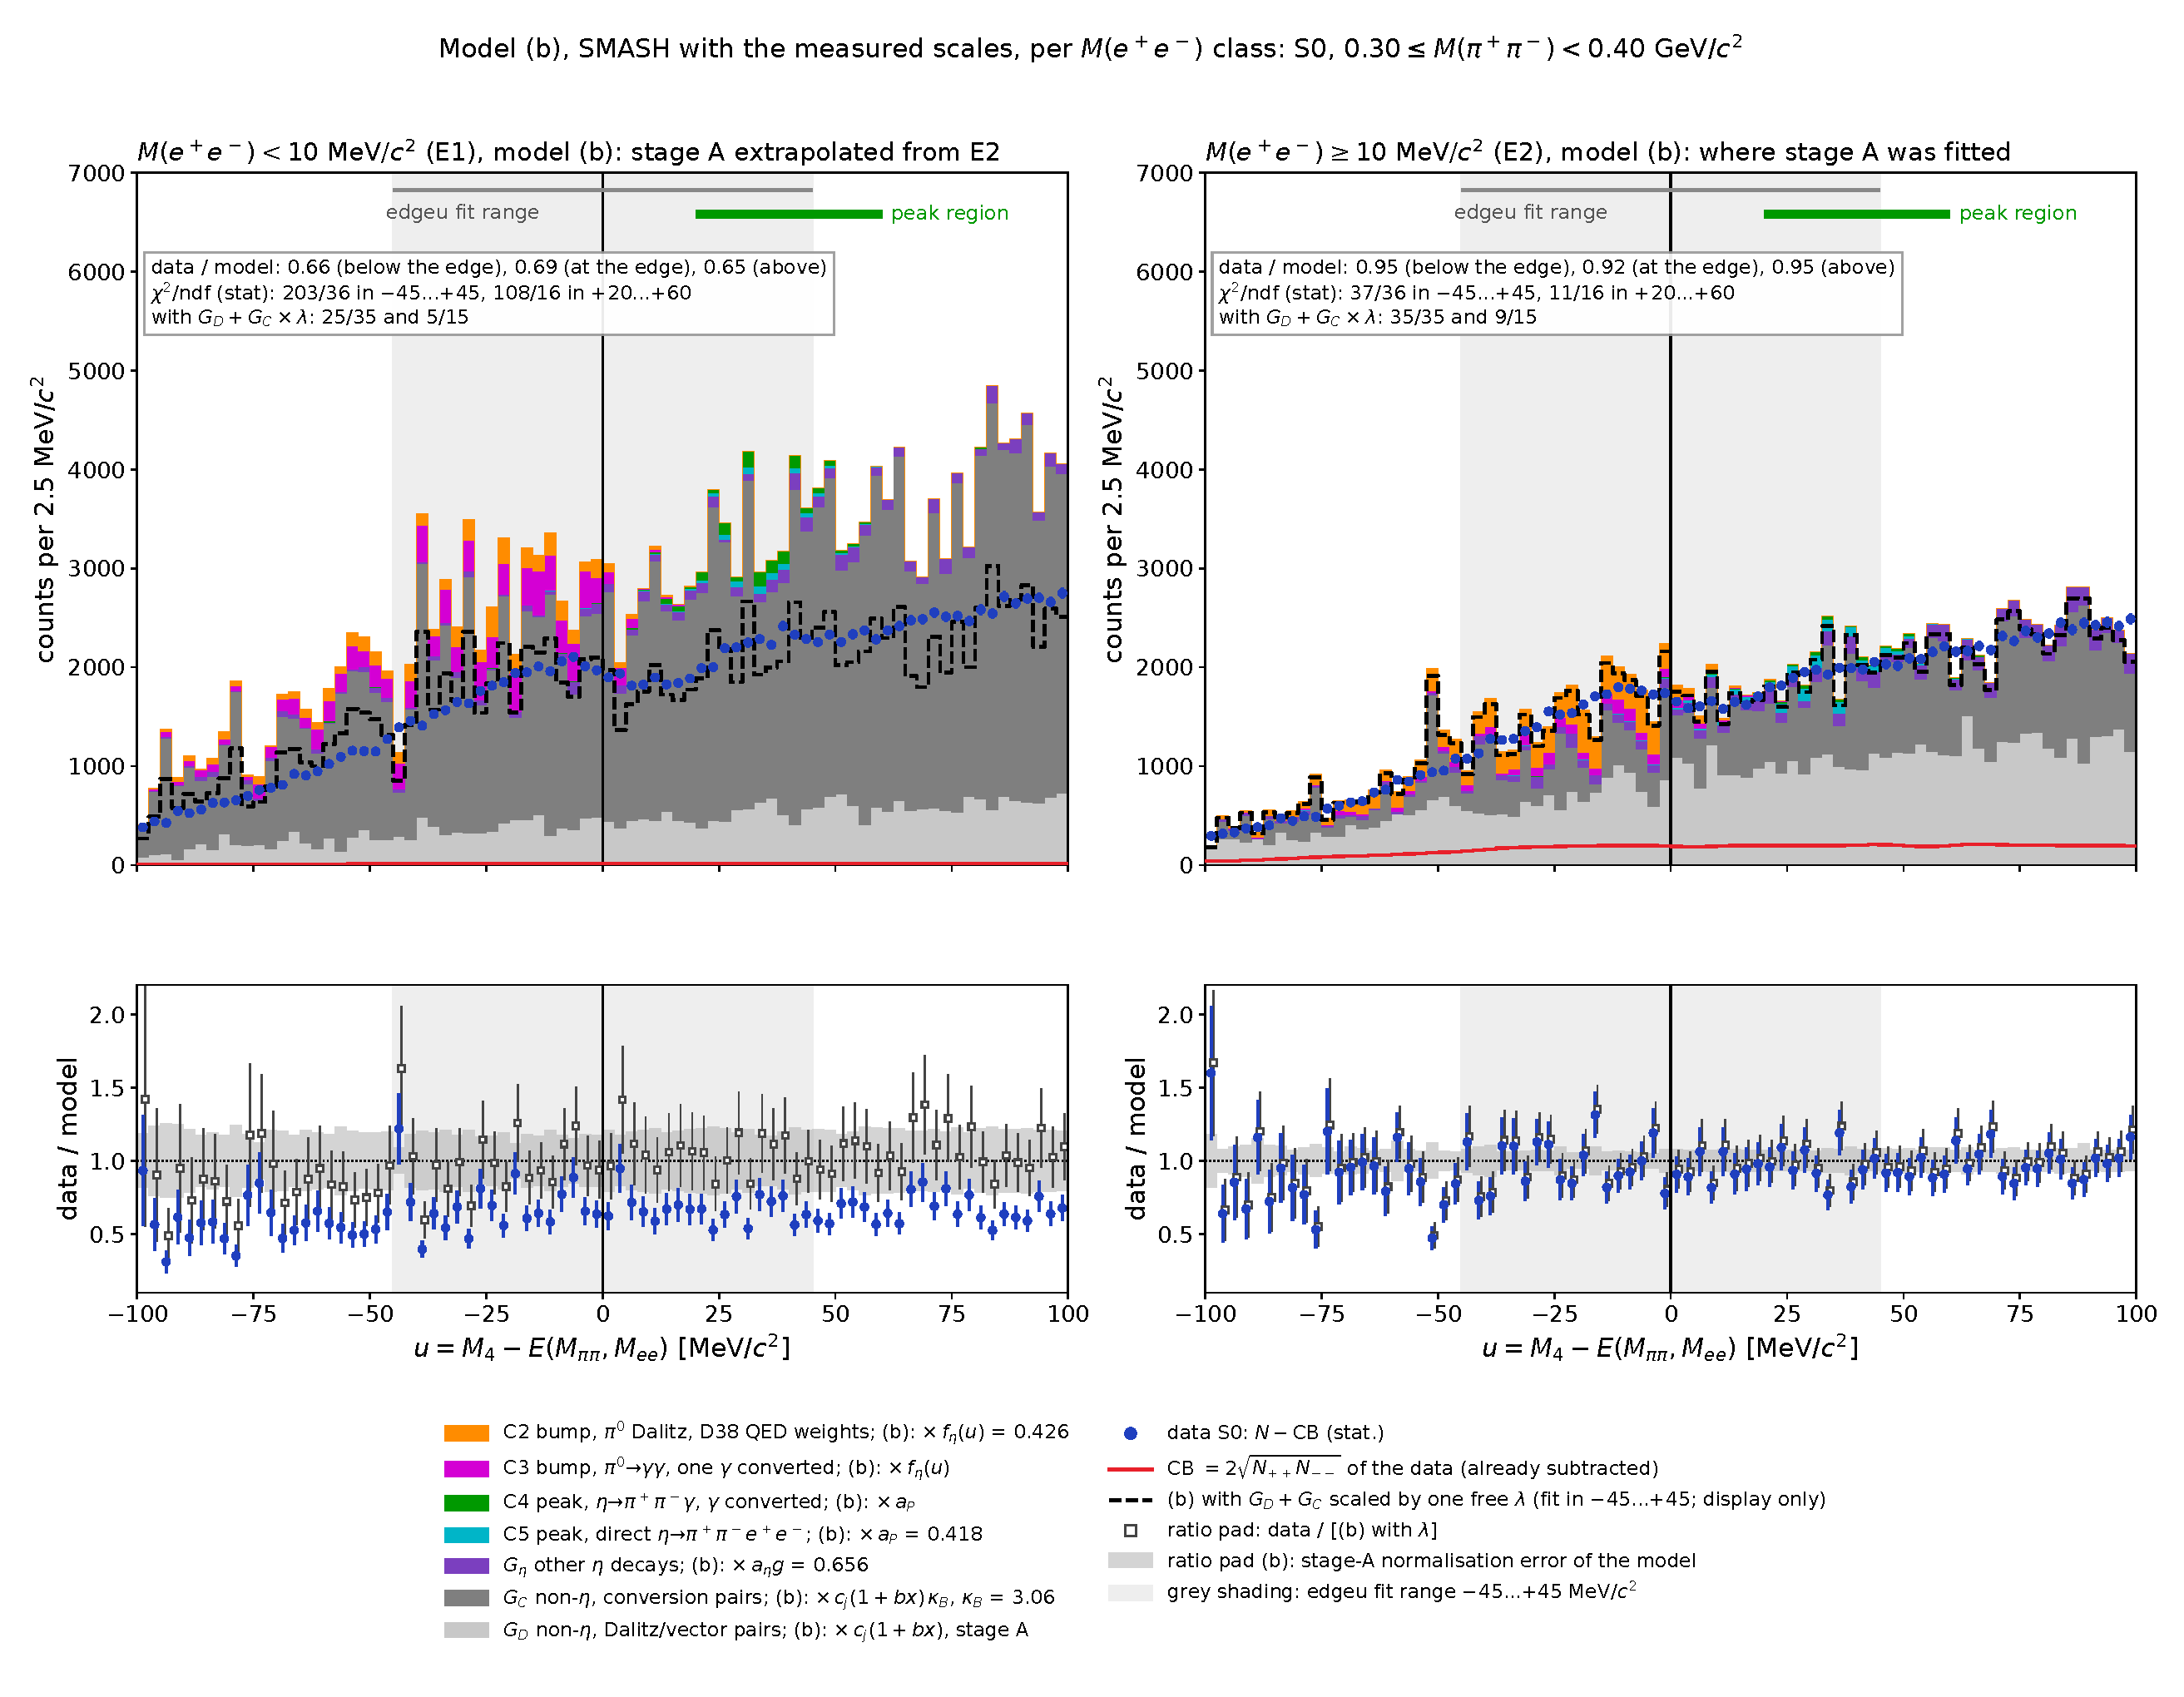
\includegraphics[width=\textwidth]{figs_all/udatasim_u_overlay_mee_v2.pdf}
\caption{\textbf{What it shows: where the background normalisation of Fig.~\ref{fig:res-after} was determined (\Mee$\ge10$\,\MeVcc, right),
SMASH with the measured scales describes the data in $u$ (data/model 0.95 / 0.92 / 0.95, $\chi^2=37/36$ and 11/16). Below 10\,\MeVcc (left) the
same normalisation puts the conversion background too high (data/model 0.65--0.69); once the background level is freed, the shape still agrees
($\lambda=0.61$, $\chi^2=25/35$).}
Selection: data at $L=6079.2\,\nbinv$ with the nominal cuts S0 (PT3 trigger; event vertex in the target region, $\vz>-160$\,mm; START-free \betanew identification, pions within 3$\sigma$, leptons within 5$\sigma$ with a RICH ring; energy-loss-corrected momenta of all four tracks; both pions used in the event-vertex fit; all stored combinations of an event, isBest $\ge0$), and SMASH with the same cuts (mode A, $w\times$V3, simulated \Mfour$\times0.99615$ and \Mpipi$\times0.9952$), $0.30\le\Mpipi<0.40$\,\GeVcc; left: \Mee$<10$\,\MeVcc; right: $10\le\Mee<135$\,\MeVcc ($u$ is defined only below the \piz mass); the CB of each \Mee class is the CB of all \Mee ($2\sqrt{N_{++}N_{--}}$ of the like-sign data in 10\,\MeVcc cells of $u$ per \Mpipi slice, $k=1$) times the like-sign share of the class in $-100\ldots+100$\,\MeVcc of $u$.
Both panels show model (b) of Fig.~\ref{fig:edgeu-sim}. Left: E1 (\Mee$<10$\,\MeVcc), stage A extrapolated from E2. Right: E2, where stage A was fitted. $0.30\le\Mpipi<0.40$\,\GeVcc; the rest
as in Fig.~\ref{fig:edgeu-sim}(b). The CB of a class is the all-class CB times the like-sign share of the class in $-100\ldots+100$\,\MeVcc (the
rule of the $u$-edge fit); in E1 the CB is 1\,\% of $N$. In E1 the conversion background $G_C$ of (b) alone (28\,198 counts below the edge) is
as large as the whole data $N-\mathrm{CB}$ there (28\,074); with the other scales fixed, the E1 data want a conversion factor of about 1.5--1.7
instead of 3.06.}
\label{fig:edgeu-sim-mee}
\end{figure}

\textbf{Checks.}
\begin{itemize}\setlength{\itemsep}{1pt}
\item \textbf{Stage A rebuilt in its own control region} (CR-U, \Mfour 0.575--0.700\,\GeVcc, E2, $N-\kEtwo\,\mathrm{CB}$ with $\kEtwo=0.954$, raw
      templates): $(N-k\,\mathrm{CB})/(B_A+0.4\,\eta)=0.990$ / 0.996 / 0.978 / 1.008 in S1--S4, $0.995\pm0.002\,(\mathrm{data})\pm0.015\,
      (\mathrm{MC})$ together. The per-count stage-A scaling with raw templates is therefore the normalisation of Fig.~\ref{fig:res-after} to
      within the template noise. S5 cannot be rebuilt (it is open-ended; the $u$ columns stop at \Mpipi$=0.46$\,\GeVcc). Stage A was fitted with
      all $\eta$ terms at 0.4 ($g=1$); with \Geta$\times0.656$, as in (b), the CR-U ratio is 0.971 (2.4\,\% lower).
\item \textbf{The peak tail (D40):} $t=0.5$ or 1.5 moves model (b) by at most 0.9\,\% per bin (at $u=+16$\,\MeVcc) and the band ratios by at most
      0.3\,\% ($\chi^2$ in the peak region 99.2 / 95.7 against 97.4); it is invisible on this display.
\item \textbf{Independent verification} (own code from the raw $u$ columns; nothing of the package reused): the data and both models agree with
      the drawn arrays bin by bin; every $\chi^2$ to 0.1 and every ratio to 0.001; $f_\eta(u)=0.42574$ and the scales of
      Table~\ref{tab:edgeu-sim-scales} confirmed. It asked for seven wording changes, all applied here and in Fig.~\ref{fig:res-udatasim}: the
      size of the level mismatch against the stage-A error; the step size, which is not a test; the weight of one simulated $G_C$ count; the level
      per \Mee class; the \Geta share; the panel titles of Fig.~\ref{fig:edgeu-sim-mee} and the \Mpipi range in the title of
      Fig.~\ref{fig:edgeu-sim-allmpp} (both figures redrawn with the corrected titles only, \code{udatasim_figs_v2.py}; same numbers).
\end{itemize}

\textbf{What not to over-read.}
\begin{enumerate}\setlength{\itemsep}{1pt}
\item \textbf{The smooth part.} The non-$\eta$ templates are raw SMASH (stage A smoothed them in \Mfour with exp(pol3); a smoothing in $u$ is not
      defined and was not done). One simulated $G_C$ count stands for about 27 expected counts, $\times3.06$ in (b), so about 84 (C2 32, \Geta 18,
      $G_D$ 13); the spikes of the stack are this template, and they lie inside the error bars of the ratio. The level of (b) at small \Mee is
      the extrapolated stage A (too high there; 1.6--1.9 standard deviations of the stage-A error); only the shape across the edge is the test.
\item \textbf{The step height in (b) is not a test} ($f_\eta$ was fitted on these bins). Tested: the step at $u=0$ with the simulated width, no
      step in any other SMASH class, the flat ratio across the edge.
\item \textbf{Cross-photon pairs} (\S\ref{sec:edgeu-ls}) end at $u=0$ too. SMASH produces such pairs (class T4, leptons from different
      sources), but they are not part of the SMASH templates used here (the compared sum $T_1+T_2$): the analysis leaves them to the CB taken
      from the data, whose $e^-e^-$ counts remove them from $N$ together with their $e^+e^-$ partners, so neither side of the ratio contains them.
\item \textbf{The peak tail (D40)} is invisible here (at most 0.9\,\% per bin).
\item \textbf{\Geta ($\times0.656$) is not a robust scale} ($g$ between 0.5 and 2.6 in Part~III); it is 3.5\,\% of model (b) in $-45\le
      u<+45$\,\MeVcc for all \Mee (5\,\% for \Mee$\ge10$\,\MeVcc, 2.4\,\% below).
\item \textbf{CB factor and scale errors.} The CB has $k=1$ (the convention of the $u$ fit); Fig.~\ref{fig:res-after} uses $\kEtwo=0.954$, which
      would raise $N-\mathrm{CB}$ by about 0.3\,\% of $N$ in E2. The errors of $f_\eta$ ($\pm0.047$) and \aP ($\pm0.080$) are not in the
      $\chi^2$ or in the bands.
\item \textbf{Colours.} $G_D$ is light grey and $G_C$ dark grey, as in Figs.~\ref{fig:res-after} and \ref{fig:C3}; the $u$ spectra of
      Fig.~\ref{fig:edgeu-spec} use the reverse greys.
\end{enumerate}
Package udatasim: \code{plots/all_report/udatasim_overlay.py} (numbers), \code{udatasim_figs.py} (figures; \code{udatasim_figs_v2.py} redraws
Figs.~\ref{fig:edgeu-sim-allmpp} and \ref{fig:edgeu-sim-mee} with the corrected titles); verifier
\code{udatasim_verify.py}, \code{udatasim_verify2.py}; outputs in \fpath{/hdd3/przygoda/HADES/FAT_out/all_report/udatasim/}.

\subsection{Caveats}
\label{sec:edgeu-cav}
\begin{enumerate}\setlength{\itemsep}{1pt}
\item \textbf{The $e^-e^-$ step} (\S\ref{sec:edgeu-ls}) comes from lepton pairs of the two \piz photons, which the CB removes as designed
      ($k_{\mathrm{cross}}=1.00\pm0.39$ from the data, independent $0.96\pm0.48$; $f$ moves by $0.0\pm1.2$\,\%, inside U5); a charge flip could
      raise $f$ by less than 1.6\,\% (1.9\,\% for either charge; 90\,\% CL); the earlier ``up to about 8\,\%'' is withdrawn (D39, approved;
      independently verified).
\item \textbf{Simulation statistics.} Only 1649 (C2) and 1187 (C3) simulated entries, 645 within 15\,\MeVcc of the edge; the MC error (7.0\,\%) is
      still larger than the statistical one (4.7\,\%).
\item \textbf{U11} rests on assumed background shapes (smoothed SMASH, stage A); the data cannot fix the cubic part across the edge better than the
      pol3 fit does ($f=0.429\pm0.037$).
\item \textbf{U2}: the data/SMASH resolution ratio is known to $\pm8$\,\% (peak width and step width combined); the variants use $\pm10$\,\%.
\item \textbf{The shape of the peak term} (\S\ref{sec:edgeu-tail}, D40). U8 varies the scale and width of the SMASH peak, not its low-mass
      tail, which reaches $u\approx0$. The tail comes from the leptons' momentum loss in the material (HGeant): the generated mass is a sharp
      line, the converter has no PHOTOS, and the conversion pairs carry the photon four-momentum (independently verified). Scaling the tail by
      $t$ moves $f$ by $+6.8$\,\% per unit $t$ (per-slice edge $+7.3$\,\%, peak side bands $+17.7$\,\%). The data do not fix $t$: the $u$ fit
      with the side-band constraint on \aP gives $t=0.0\pm0.9$ to $0.6\pm1.0$, depending on the treatment of the C4 entries. The line shape at
      $\Mpipi\ge0.42$\,\GeVcc cannot separate the tail from a 1\,\MeVcc peak shift. Part~II's Gaussian peak term (no tail; amplitude
      $2838\pm717$) gives an $f$ 8.6\,\% lower: about $-4.7$\,\% from the missing tail (the same Gaussian at the SMASH positions; the SMASH
      peak without its tail gives $-5.8$ to $-6.9$\,\%) and $-3.9$\,\% from the side-band peak positions, which
      lie 1.0\,\MeVcc later in $u$ than SMASH's (not understood). A peak without a tail is excluded by physics (the material exists, and the
      decay radiates, adding about 10\,\% to the tail, which SMASH lacks), not by the data. Counted: $t=1\pm0.5$, i.e.\ $\pm3.4$\,\% (D40, approved).
\item \textbf{The C2 $\gamma^*$ factor} is applied per count (D38, approved; 0.861 for this fit, \S\ref{sec:c2recon}): $f=0.426$ instead of
      0.420 with the constant factor of D35 (a toy at the $u$-edge itself gave 0.879 for the SMASH E1/E2 mix of the C2 step, against the 0.881 of
      that constant factor).
\item \textbf{Folds} ($z=-2.1$) and \textbf{periods} ($p=0.024$) are marginal; they point to the same data feature as per slice, and the fit in
      $u$ does not remove it.
\item The mean of the simulation replicas of $h_{\mathrm{sim}}$ is 1\,\% below the nominal (the WP0 replica set; the verifier's independent set is
      0.35\,\% above): information only.
\item Combinations with \Mee$\ge m_{\piz}$ have no defined $u$ and are not used; no bump combination is lost.
\item \textbf{Blinding}: only the \Mee classes $<10$, $\ge10$ and $\ge20$\,\MeVcc were formed in the data; \Mee enters $u$ only through $E$, combination
      by combination; no X17 cell and no fine \Mee shape were made.
\item \textbf{The absolute \sigeta} inherits the PRELIMINARY label of Part~III; the one-sided items are not included.
\end{enumerate}

\textbf{Verification} (vedgeu, own code: own pass over the entries of the data and simulated trees, own edge function, CB rule, step template, iterated fit,
bootstrap and replica generators; shared by design only the frozen definitions and the typed Part~III inputs). Every decisive number is
reproduced almost to the last digit: $h_{\mathrm{data}}=1305.05\pm62.27$, $\chi^2=27.34/32$ (466.6 without the step), $h_{\mathrm{sim}}=3106.95$,
$f=0.4200\pm0.0200$, 0.3899 uncorrected, 0.5400 with the conversions $\times0.48$; stat (own bootstrap) 0.0202, MC (own replicas) 0.0259, so the
quoted MC (0.0292) is on the safe side. A brute-force scan of the photon direction reproduces $M_4^{\max}(m,q)$ to $10^{-6}$\,\GeVcc; nine
variants, the null tests, the classes, slices, periods, yields and \sigeta agree; the pseudo-data claim holds ($q$ term $-2.0$\,\%; narrow
structures $+7.0$ and $+16.6$\,\%; pull widths 0.99--1.02). Four statements of the first note needed other words, none changes a number, and all
are corrected above: the comparison with the per-slice edge (like for like 11.9 $\to$ 11.1\,\% before D40, stat about 8\,\% smaller, not 13\,\%); the double
ratio ($\pm0.37$ with the composition term, not $\pm0.22$); the $e^-e^-$ step (``only at \Mee$\ge10$'' and ``mostly period I'' not significant;
its size is); \Geta (raw step $123\pm53$, treated as noise). Further: the core width is method dependent (template width, not a measured
resolution); the dashed line of the fit figure is the smooth part, not the background; Fig.~\ref{fig:edgeu-syst} does not show U11.
\textbf{Verdict: CONFIRMED.}

\notebox{\textbf{D37 (lead analysis, approved by the analyst on 15 November 2026).} The bump is measured in $u=\Mfour-E(\Mpipi,\Mee)$: the
$u$-edge is \emph{the} bump measurement, $f_\eta(u\text{-edge})=0.426\pm0.020\,(\mathrm{stat})\pm0.034\,(\mathrm{syst})\pm0.030\,(\mathrm{MC})$ and
\sigeta from the bump $0.444\pm0.021\pm0.035\pm0.031\,^{+0.043}_{-0.044}$\,mb (with the per-count C2 weights of D38 and the peak-tail family of D40);
the per-slice edge (D35, \S\ref{sec:bedge}) is the cross-check. Reasons: one step instead of four, the \Mee term of the edge exact, the simulated
step from the bump classes alone, and a like-for-like total error of 11.6 against about 12.4\,\% (11.1 against 11.9\,\% before D40); not a reason:
the model dependence, which is the same. The headline \sigeta $=0.429$\,mb from the peak side bands is
unchanged.}

%======================================================================
\section{Full reconstruction of the bump with the ECAL photon}
\label{sec:ecalacc}
%======================================================================
\inshort{a feasibility study, not a measurement. One third of the lost bump photons hit an active ECAL module (ECAL sector 0 is off; the
modules cover 10.9--45.6$^\circ$ seen from the target centre), but the photon is soft, so about 10\,\% of the bump is fully reconstructed in the
simulation (14\,\% at a data-like energy scale) and about 12\,\% in the data, as a clean peak. The data hold $1.16\pm0.21$ of the prediction with
the simulated photon-energy scale and $0.84\pm0.15$ with a data-like one: the photon energy scale, the module efficiency, a START-free photon cut
and more simulation are needed before the tag can be a measurement. The acceptance itself is known and the same in data and simulation.}

\subsection{What was done}
\label{sec:ecalacc-proc}
The ECAL tag of Part~II ($T=3314\pm105$ counts for ``pre'', $3090$ for S0) counts the combinations in which the ECAL sees the photon that the bump has lost,
so that the whole $\eta\to\pipi\piz$ is reconstructed (good photon, $0.119\le M(\ee\gamma)<0.173$\,\GeVcc, \Mee$<0.10$\,\GeVcc, frozen fit of
$m_{5c}$). The question here is how much of the bump this full reconstruction can see, and what must be known before it can be a measurement.
\begin{enumerate}\setlength{\itemsep}{1pt}
\item \textbf{The ECAL coverage} was read from the geometry (EmcGeomPar) and module status (EmcCellStatusPar) of the parameter file of the gen4
      simulation production (on vae25, read only), and the same status from the data parameter file at eight runs of the four periods (first runs of
      days 034, 039, 045, 047, 049, 053, 059, 067).
\item \textbf{The lost photon, recovered.} The simulation does not store the photon of a simulated bump entry, but the four charged momenta (true), the \piz
      mass and the $\eta$ mass leave it on a known circle; its position on the circle follows the SMASH $\eta$ momentum spectrum (read from the
      SMASH event files) and the decay matrix element (flat in HGeant). So every simulated bump entry gets the full distribution of the direction and
      energy of its photon (``conditional completion'').
\item \textbf{Fractions} for the accepted simulated bump entries C2+C3 (2836 in ``pre''): photon in an active module, above the 100\,MeV cluster cut,
      found by the ECAL simulation, combination fully reconstructed; against \Mpipi, the photon energy and the distance to the edge.
\item \textbf{Prediction for the data}: the simulated tag scaled with the measured $\eta$ scale of the bump edge, also with the simulated cluster
      energies $\times\lambda$ ($\lambda=1.10$, 1.20, 1.285 = data-like), and with two data-only effects (the wider \piz of the data and the START
      dependence of the photon $\beta$ cut).
\end{enumerate}

\subsection{The acceptance: geometry, module status and the lost photon}
\label{sec:ecalacc-acc}
\textbf{Geometry and status} (Table~\ref{tab:ecalacc-geo}, Fig.~\ref{fig:ecalacc-geo}). Six sectors of 163 lead-glass modules (front
$92\times92$\,mm, pitch 94\,mm, depth 420\,mm, front planes 2357--2411\,mm from the target). \textbf{ECAL sector 0} (azimuth 63--117$^\circ$, the
azimuth of tracking sector 0; the sector-2 trigger deficit of \S\ref{sec:norm} is at 180--240$^\circ$) is switched off completely, and 8 single
modules are dead: 807 of 978 modules are active. The status map is identical in the simulation and in the data at all eight runs. Seen from the
target centre ($z\approx-124$\,mm; the simulated vertex is uniform in $-148$ to $-99$\,mm, the data median is $-125$\,mm) the module corners span
10.9--45.6$^\circ$ in polar angle; the active modules cover 8.45\,\% of $4\pi$ (10.3\,\% with six working sectors). (The first note quoted
11.5--47.5$^\circ$ and 9.2\,\%, which hold from $z=0$, not from the target.) At a given polar angle a working sector covers 45--53$^\circ$ of its
60$^\circ$ in azimuth (the 54$^\circ$ of the corner extent is reached nowhere). The simulated photons that make a cluster point to 11.75--44.3$^\circ$
(0.1--99.9\,\% quantiles), and the clusters occupy exactly the 807 active modules: geometry, status and the cell mapping agree.

\begin{table}[H]
\centering
\caption{\textbf{What it shows: ECAL sector 0 is off and 8 single modules are dead, in the simulation and in the data alike; seen from the target
centre the modules span 10.9--45.6$^\circ$.} ECAL geometry and status of the gen4 simulation parameter file (identical status in the data at eight
runs of the four periods); polar angles of the module corners from $z=0$ and from the target centre $z=-124$\,mm, azimuth from $z=0$. Corrected
version of \code{ecalacc_geometry.tex} (whose second column was from $z=-60$\,mm and whose 9.2\,\% is the coverage from $z=0$), written from the
verifier's geometry dump by \code{plots/all_report/ecalacc_geometry_v2.py}.}
\label{tab:ecalacc-geo}
\footnotesize
\resizebox{\textwidth}{!}{\tabin{ecalacc_geometry_v2.tex}}
\end{table}

\begin{figure}[!htbp]
\centering
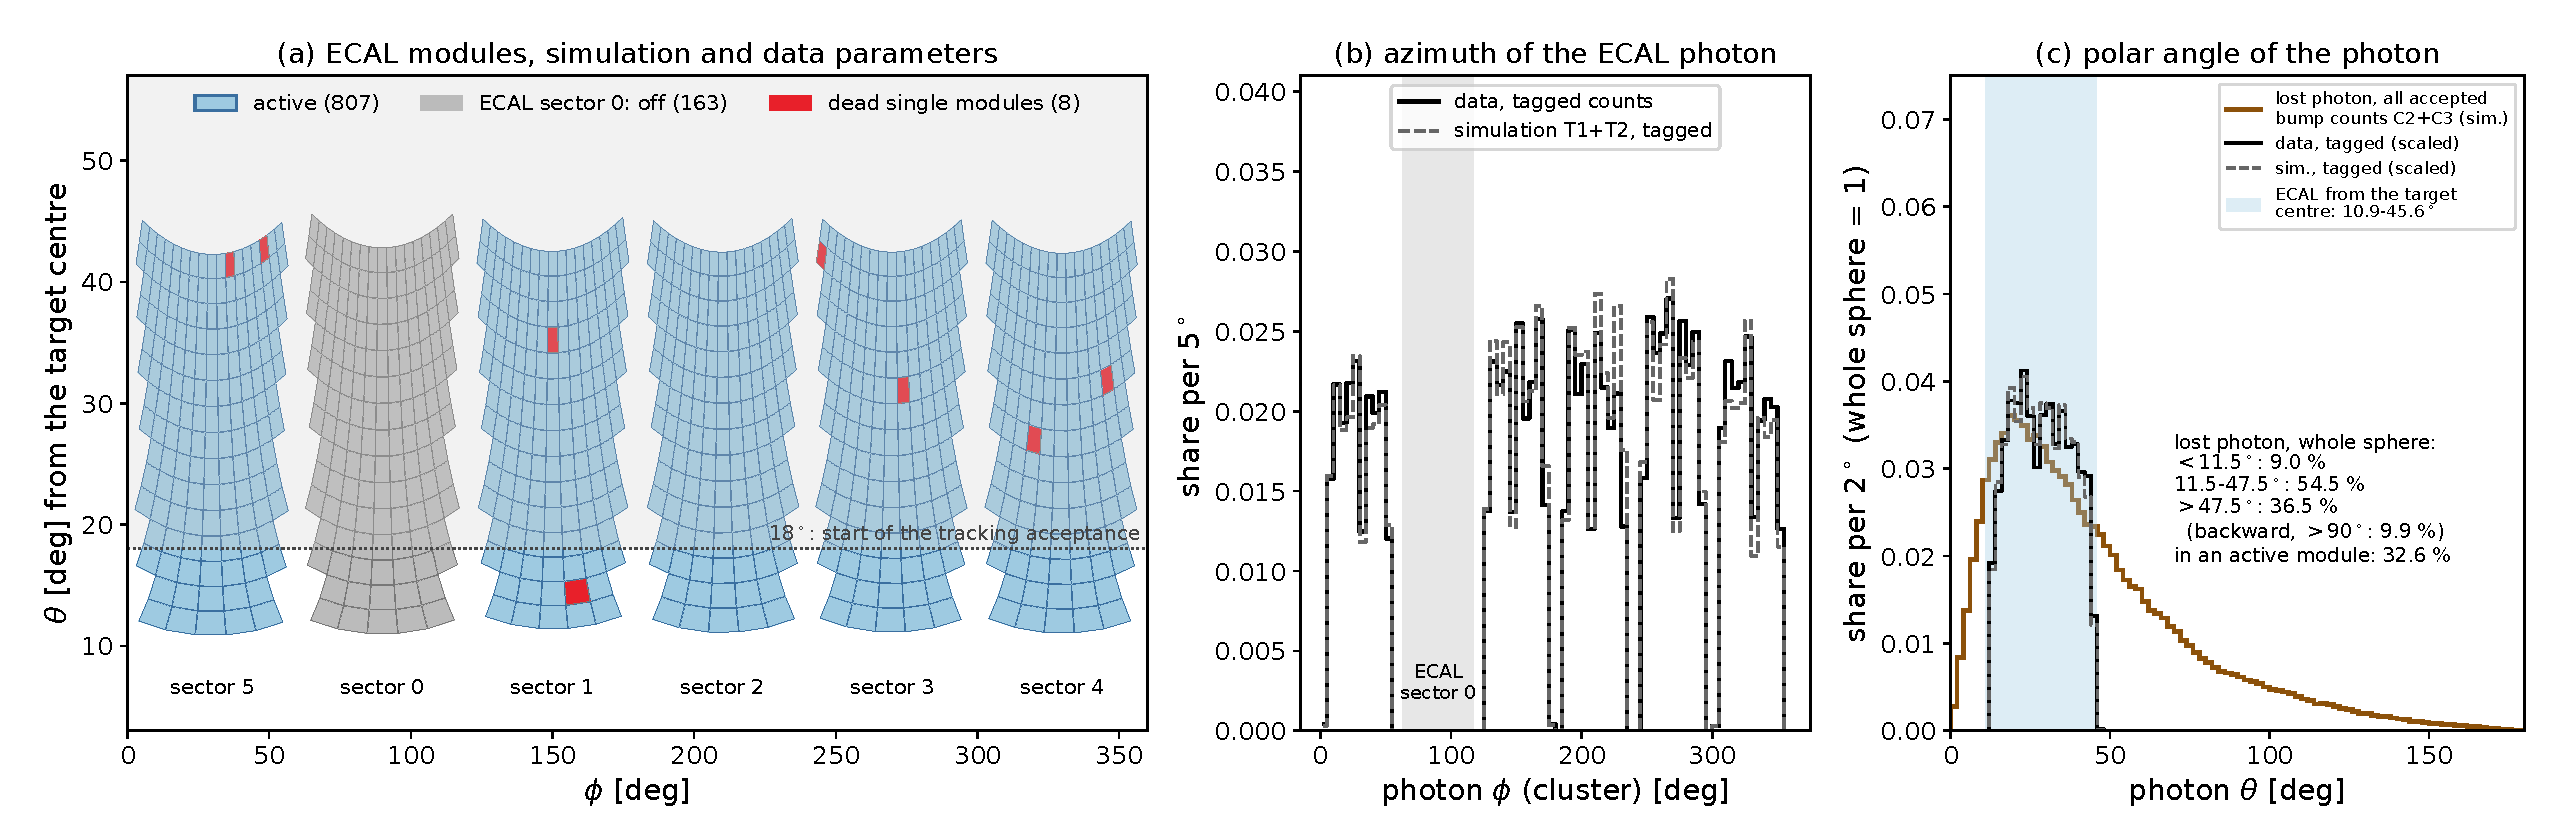
\includegraphics[width=\textwidth]{figs_all/ecalacc_geometry_v2_cnt.pdf}
\caption{\textbf{What it shows: the ECAL covers 10.9--45.6$^\circ$ in polar angle, seen from the target centre, in five of its six sectors; the
data photons fill exactly this coverage, as the simulated ones do, and two thirds of the lost bump photons fly outside it.}
Selection: (a) no event selection: the ECAL geometry and module status of the gen4 simulation parameter file (the same status in the data parameter files at eight runs of the four periods). (b), (c) black: data with the base cuts ``pre'' (PT3 trigger; event vertex in the target region, $\vz>-160$\,mm; START-free \betanew identification, pions within 3$\sigma$, leptons within 5$\sigma$ with a RICH ring; energy-loss-corrected momenta of all four tracks; all stored combinations of an event, isBest $\ge0$; no condition on the pions in the event-vertex fit) and an ECAL photon tag: a good ECAL photon (identified as a photon, $0.8<\beta<1.2$, cluster energy above 100\,MeV; of up to three, the one with $M(\ee\gamma)$ closest to 0.140\,\GeVcc), $0.119\le M(\ee\gamma)<0.173$\,\GeVcc and \Mee$<0.10$\,\GeVcc, all \Mfour, raw counts of the unlike-sign tagged combinations (no CB subtracted); grey dashed: the same cuts on SMASH $T_1+T_2$ ($\eta$ signal and physical background: a true \ee pair from one source), mode A, $w\times$V3. Brown in (c): the true lost photon of all simulated bump counts C2+C3 that pass ``pre'', with no ECAL condition.
(a) The 978 ECAL modules seen from the target centre ($z=-124$\,mm), from the geometry and module status of the gen4 simulation parameter file:
light blue active (807), grey ECAL sector 0, switched off (163), red dead single modules (8); the data parameters of all four periods have the same
status; dotted: 18$^\circ$, where the tracking acceptance starts. (b) Azimuth of the ECAL photon of the tagged combinations (good photon,
$0.119\le M(\ee\gamma)<0.173$\,\GeVcc, \Mee$<0.10$\,\GeVcc, ``pre''): data (black) and simulation $T_1+T_2$ (grey dashed), each normalised to 1;
grey band: ECAL sector 0. (c) Polar angle over the whole sphere: brown, the true lost photon of all accepted bump combinations C2+C3 (conditional
completion, SMASH $\times$ V3; whole sphere $=1$: 9.0\,\% below 11.5$^\circ$, 54.5\,\% in 11.5--47.5$^\circ$, 36.5\,\% above, 9.9\,\% backward);
black / grey dashed: the cluster polar angle of the tagged combinations in data and simulation, scaled to the brown share in 12--48$^\circ$; blue band: the
ECAL seen from the target centre. Redrawn from the package figure \code{ecalacc_geometry.pdf} with the corrections of the verification (whole
sphere instead of $\theta<90^\circ$; target centre instead of $z=0$) and in colours that are not the class colours of Part~III
(\code{plots/all_report/ecalacc_geometry_v2.py}).}
\label{fig:ecalacc-geo}
\end{figure}

\textbf{The lost photon} (Table~\ref{tab:ecalacc-frac}, Figs.~\ref{fig:ecalacc-frac}, \ref{fig:ecalacc-energy}). Over the whole sphere, 9.0\,\% of
the lost photons of the accepted bump combinations fly below the ECAL band ($<11.5^\circ$), 54.5\,\% into it and 36.5\,\% above it, 9.9\,\% of them backward
(the first note gave 11 / 60 / 29\,\%, normalised to the forward photons only; the share in the tracking range 18--85$^\circ$ is 68.9\,\%, not
76\,\%). \textbf{32.7}\,$\pm$\,0.4\,\% hit an active module (40.3\,\% with six working sectors), the same for C2 and C3, in ``pre'' and S0, and flat in
\Mpipi. The photon is soft: mean true energy 130\,MeV (172\,MeV inside the modules), 51\,\% below 100\,MeV. Only 21.6\,\% of the combinations have their photon
in a module \emph{and} above 100\,MeV, 13\,\% near the edge (where the photon takes the smallest possible energy) and 34\,\% far below it. Inside the
active modules the ECAL simulation finds a cluster of the true photon in about 65\,\% of the cases, at all energies (not explained; known part:
about 4\,\% of the combinations have a cluster made by an $e^\pm$ of a converted photon); with the quality cuts (neutral candidate, $0.8<\beta<1.2$,
$E_{\mathrm{cluster}}>100$\,MeV) 38\,\%, nothing below 80\,MeV and 60--75\,\% above 160\,MeV. Fully reconstructed (tag with the true photon, $m_{5c}$
in 0.49--0.62\,\GeVcc) are \textbf{9.8}\,$\pm$\,0.6\,\% of the accepted bump combinations (14.1\,\% with the cluster energies $\times1.285$): 6.9\,\% (11\,\%) near
the edge, 8.4\,\% (13\,\%) in window B and 16\,\% (20\,\%) far below the edge. The tagged combinations therefore sit \emph{preferentially}, not mainly, below
the edge: 27.5\,\% of the tagged weight lies more than 60\,\MeVcc below it (bump: 16.5\,\%), 46.7\,\% between $-60$ and $-20$\,\MeVcc (44.9\,\%) and
25.8\,\% above $-20$\,\MeVcc (38.2\,\%); tag and edge weight the same bump differently. The tag is specific to the bump: 12.7\,\% of the bump combinations are
tagged, 0.78\,\% of C4 and 1.78\,\% of C5 (the peak classes make about 2.2\,\% of the simulated tagged weight). In the data the tag finds about
$3314/28\,700\approx12$\,\% of the visible bump.

\begin{table}[H]
\centering
\caption{\textbf{What it shows: one third of the lost photons hit an active module, about one fifth also carry more than 100\,MeV, and about one
tenth of the bump combinations is fully reconstructed, fewer near the edge.} Simulation, accepted bump combinations ``pre'' (SMASH $\times$ V3, expected raw
counts), per cent; window B and ``edge'' ($-15$ to $+5$\,\MeVcc from the edge). MC errors: 0.4--0.6 points for C2+C3 (Sect.~2.2 of the note).
Source: \code{tables_all/ecalacc_results.txt}.}
\label{tab:ecalacc-frac}
\footnotesize
\tabin{ecalacc_results.tex}
\end{table}

\begin{figure}[!htbp]
\centering
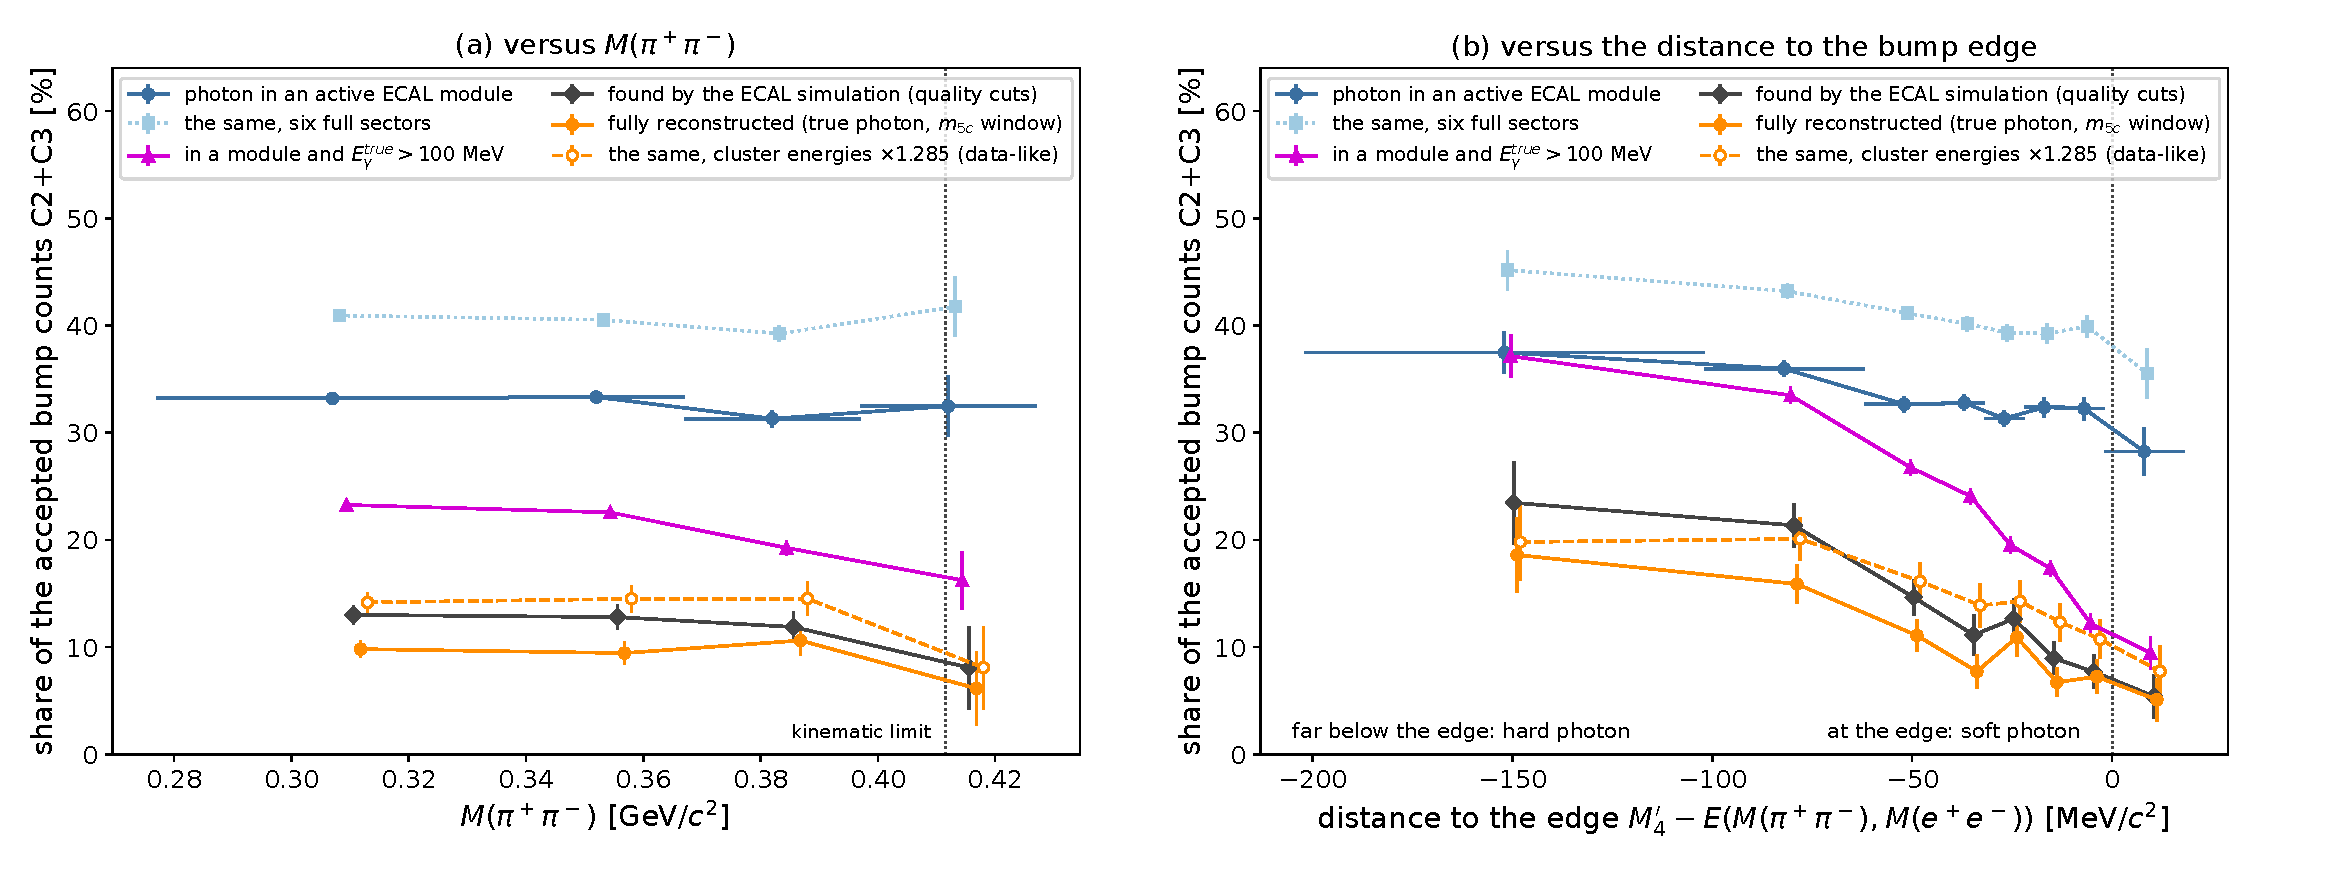
\includegraphics[width=\textwidth]{figs_all/ecalacc_fractions_cnt.pdf}
\caption{\textbf{What it shows: one third of the lost bump photons hit an active ECAL module at every \Mpipi, but near the edge the photon is too
soft for the 100\,MeV threshold, so the full reconstruction sees preferentially the part of the bump below the edge.}
Selection: simulation only: the simulated bump classes C2+C3 ($\eta\to\pipi\piz$, $\piz\to\ee\gamma$ or one \piz photon converted, the other photon lost; standard set, mode A, $w\times$V3, expected raw counts at 6079.2\,\nbinv) that pass the base cuts ``pre'' (PT3 trigger; event vertex in the target region, $\vz>-160$\,mm; START-free \betanew identification, pions within 3$\sigma$, leptons within 5$\sigma$ with a RICH ring; energy-loss-corrected momenta of all four tracks; all stored combinations of an event, isBest $\ge0$; no condition on the pions in the event-vertex fit); 2836 simulated entries; the lost photon of each count from the conditional completion; ``fully reconstructed'' means an ECAL photon tag: a good ECAL photon (identified as a photon, $0.8<\beta<1.2$, cluster energy above 100\,MeV; of up to three, the one with $M(\ee\gamma)$ closest to 0.140\,\GeVcc), $0.119\le M(\ee\gamma)<0.173$\,\GeVcc and \Mee$<0.10$\,\GeVcc, the tagged photon being the true lost photon, and $m_{5c}$ (mass of \ppee and the photon, the photon energy rescaled to $M(\ee\gamma)=m_{\piz}$) in 0.49--0.62\,\GeVcc. In (a) \Mpipi is on the data scale ($\times0.9952$); in (b) the distance to the edge uses \Mfour$\times0.99615$.
Simulation, accepted \ppee combinations of the bump classes C2+C3, ``pre'', SMASH $\times$ V3, MC errors. Blue: photon in an active module; light blue:
the same with six full sectors; magenta: in a module and true energy above 100\,MeV; dark grey: found by the ECAL simulation with the quality cuts;
orange: fully reconstructed (true photon, $m_{5c}$ in 0.49--0.62\,\GeVcc); orange open, dashed: the same with the simulated cluster energies
$\times1.285$ (data-like). (The magenta and orange of this figure are not the classes C3 and C2.) (a) Against \Mpipi (data scale; dotted: the
kinematic limit 0.4116\,\GeVcc). (b) Against the distance to the edge, $M_4'-E(\Mpipi,\Mee)$, i.e.\ $u$ of \S\ref{sec:edgeu}.}
\label{fig:ecalacc-frac}
\end{figure}

\begin{figure}[!htb]
\centering
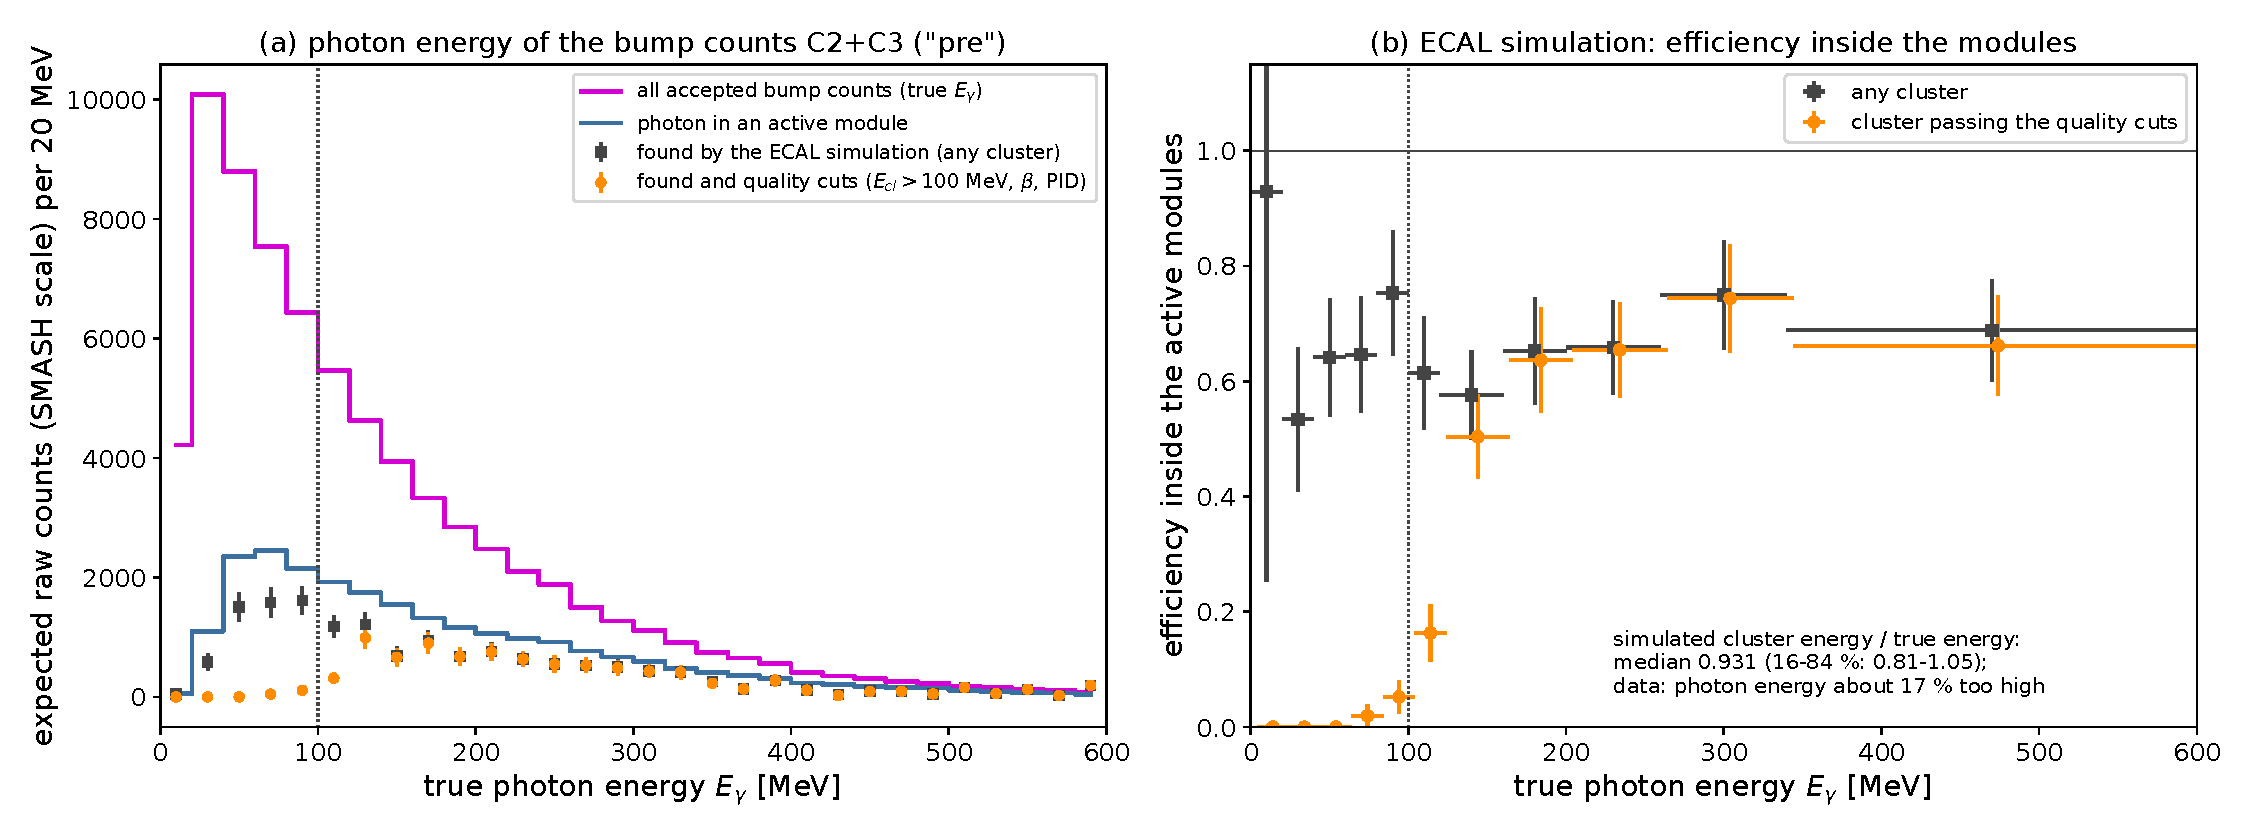
\includegraphics[width=\textwidth]{figs_all/ecalacc_energy_cnt.pdf}
\caption{\textbf{What it shows: half of the lost photons have less than 100\,MeV; inside the modules the simulated ECAL finds a cluster for about
65\,\% of them at every energy, but the quality cuts remove almost everything below 120\,MeV.}
Selection: simulation only, as in Fig.~\ref{fig:ecalacc-frac}: the simulated bump classes C2+C3 ($\eta\to\pipi\piz$, $\piz\to\ee\gamma$ or one \piz photon converted, the other photon lost; standard set, mode A, $w\times$V3, expected raw counts at 6079.2\,\nbinv) that pass the base cuts ``pre'' (PT3 trigger; event vertex in the target region, $\vz>-160$\,mm; START-free \betanew identification, pions within 3$\sigma$, leptons within 5$\sigma$ with a RICH ring; energy-loss-corrected momenta of all four tracks; all stored combinations of an event, isBest $\ge0$; no condition on the pions in the event-vertex fit); (a) magenta and blue: true photon energy from the conditional completion, all and with the photon in an active module; grey: any ECAL cluster of the true photon; orange: that cluster passes the quality cuts (identified as a photon, $0.8<\beta<1.2$, cluster energy above 100\,MeV).
(a) True photon energy of the accepted bump combinations C2+C3 (``pre''): all (magenta) and in an active module (blue), from the conditional completion;
photons found by the ECAL simulation (any cluster: grey; passing the quality cuts PID 1, $0.8<\beta<1.2$, $E_{\mathrm{cluster}}>100$\,MeV: orange),
from the cluster truth. (b) Efficiency inside the active modules (found / in a module) against the true energy. The simulated cluster energy is
7--9\,\% low (median $E_{\mathrm{cluster}}/E_{\mathrm{true}}=0.931$ for clusters passing the cuts); the data photon energy is about 17\,\% high
(Part~II). (Magenta and orange are not the classes C3 and C2 here.)}
\label{fig:ecalacc-energy}
\end{figure}

\subsection{Closure of the photon prediction}
\label{sec:ecalacc-closure}
For the 598 simulated entries in which the ECAL simulation found the photon (cluster truth: a photon from the same \piz), the photon lies on the predicted
circle ($|\Delta\cos\alpha|<10^{-3}$ for 99.8\,\%), and 99.5\,\% of them hit an active module of the geometry test (0.33\,\% a dead module, the cluster
landing in a neighbour; one photon outside). The predicted hit probability is calibrated: entries with a higher predicted probability have
proportionally more found photons, with the same ratio 0.64--0.68 in every bin (this ratio is the efficiency inside the modules), so the
distribution of the photon direction along the circle is right. The simulated cluster energy is low: $E_{\mathrm{cluster}}/E_{\mathrm{true}}$ (16 /
50 / 84\,\%) $=0.752$ / 0.914 / 1.043 for all found photons and 0.808 / 0.931 / 1.048 after the quality cuts (Fig.~\ref{fig:ecalacc-closure}).

\begin{figure}[!htbp]
\centering
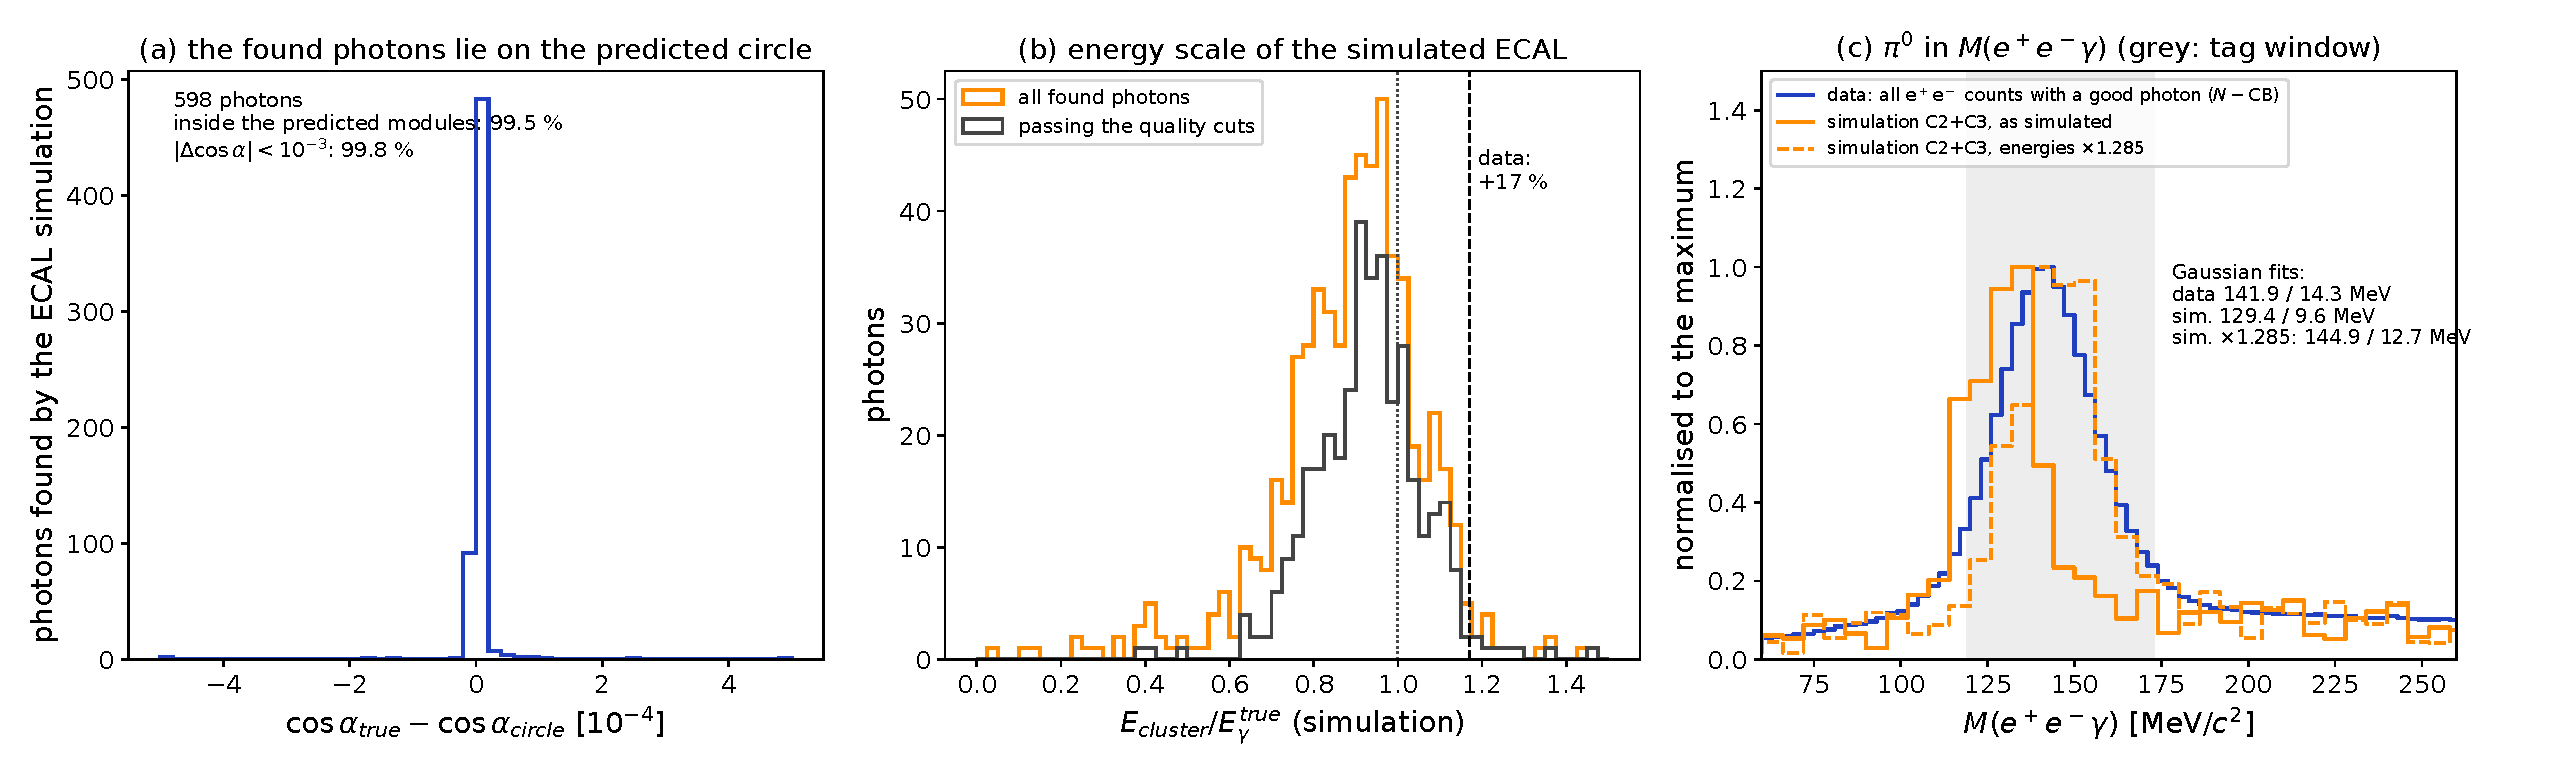
\includegraphics[width=\textwidth]{figs_all/ecalacc_closure_cnt.pdf}
\caption{\textbf{What it shows: the photon predicted for each bump combination is the photon that the ECAL simulation finds, and the ECAL energy scale differs
between data and simulation.}
Selection: (a), (b) simulation only: the 598 counts, among the simulated bump classes C2+C3 ($\eta\to\pipi\piz$, $\piz\to\ee\gamma$ or one \piz photon converted, the other photon lost; standard set, mode A, $w\times$V3, expected raw counts at 6079.2\,\nbinv) that pass the base cuts ``pre'' (PT3 trigger; event vertex in the target region, $\vz>-160$\,mm; START-free \betanew identification, pions within 3$\sigma$, leptons within 5$\sigma$ with a RICH ring; energy-loss-corrected momenta of all four tracks; all stored combinations of an event, isBest $\ge0$; no condition on the pions in the event-vertex fit), in which the ECAL simulation found the photon (a cluster of a photon from the same \piz); in (b) orange: all of them, grey: those whose cluster passes the quality cuts (identified as a photon, $0.8<\beta<1.2$, cluster energy above 100\,MeV). (c) Data with ``pre'' (cuts as above), all \Mfour, \Mee$<0.10$\,\GeVcc and a good ECAL photon (identified as a photon, $0.8<\beta<1.2$, cluster energy above 100\,MeV; of up to three, the one with $M(\ee\gamma)$ closest to 0.140\,\GeVcc), no $M(\ee\gamma)$ window: $N-\mathrm{CB}$ with CB $=2\sqrt{N_{++}N_{--}}$ of the like-sign data bin by bin in $M(\ee\gamma)$; simulation: the bump counts C2+C3 with the same cuts; each curve normalised to its maximum in 60--240\,\MeVcc.
(a) For the 598 photons found by the ECAL simulation: $\cos\alpha$ of the true photon minus the predicted $\cos\alpha$ of the circle ($\alpha$ = angle
to $P=\ppee$ in the \ee rest frame). The axis spans only $\pm5\times10^{-4}$; 99.8\,\% of the photons lie within $10^{-3}$, so only 0.2\,\% are outside
twice the range shown. (b) Simulated $E_{\mathrm{cluster}}/E_{\mathrm{true}}$ for all found photons (orange) and those passing the quality cuts (grey);
dashed: the data scale ($+17$\,\%). (c) \piz in $M(\ee\gamma)$: data, all \ee combinations with a good photon, $N-\mathrm{CB}$ (blue); simulation C2+C3 as
simulated (orange) and with the cluster energies $\times1.285$ (orange dashed); grey: the tag window 0.119--0.173\,\GeVcc.}
\label{fig:ecalacc-closure}
\end{figure}

\subsection{Data against the prediction}
\label{sec:ecalacc-data}
\textbf{The data side} (data only). The tagged photons of the data have the same azimuth and polar-angle distributions as the simulated ones, bin
by bin; ECAL sector 0 is empty in both (Fig.~\ref{fig:ecalacc-geo}b, c). $T(\mathrm{pre})=3314\pm105$, $T(\mathrm{S0})=3090$ (the frozen fit is
reproduced exactly). \textbf{Photon energy scale in the data}: about 17\,\% too high, measured by the factor that rescales each tagged photon so that
$M(\ee\gamma)=m_{\piz}$ (median 0.856); the \piz of the tagged $\eta$ sits at $146.0\pm0.5$\,\MeVcc (width 13.7\,\MeVcc), 8\,\% above $m_{\piz}$, and
all \ee combinations with a good photon give 141.9\,\MeVcc (width 14.3); the simulation gives 129.4\,\MeVcc (width 9.6), and 144.9\,\MeVcc (12.7) with
its cluster energies $\times1.285$. The 100\,MeV cluster cut therefore sits near 85\,MeV true energy in the data and near 108\,MeV in the
simulation. \textbf{START}: the photon $\beta$ cut (0.8--1.2) uses the START time in the data. The 6.4\,\% of the \ee combinations without a START hit
(7.2\,\% in window B) are tagged at only $0.80\pm0.12$ (all \Mfour) or $0.69\pm0.11$ (window B) of the normal rate ($T$ with START $3145\pm102$,
without $170\pm26$); this costs $T$ 1.4\,\% (with the all-\Mfour share) to 2.3\,\% (with the window-B share). The simulation always has a START hit.

\textbf{The prediction.} $T_{\mathrm{exp}}=f_\eta(\mathrm{edge})\times T_{\mathrm{sim}}\times$ composition $\times$ calibration, with
$T_{\mathrm{sim}}=7295$ (``pre'', frozen fit on the simulated $T_1+T_2$; 23\,\% of the simulated C2+C3 tags in the window use a wrong photon, but the
fit counts essentially the true-photon tags, 7175). As simulated: $2857\pm153\,(\mathrm{stat})\pm234\,(\mathrm{syst})\pm400\,(\mathrm{MC})$, data/expected
$=1.16\pm0.21$; C2-corrected ($0.423\times$ composition 0.928, with the C2 factor 0.876 of the tagged combinations) 2866 (1.16; 2832 and 1.17 with the
constant factor of D35) and with the conversions $\times0.48$ 2952 (1.12; 2905 and 1.14). The calibration of the simulated tag grows with the
cluster energy scale: $\times1.245$ at $\lambda=1.10$, $\times1.374$ at 1.20, $\times1.464$ at 1.285 (data/expected 0.93, 0.84, 0.79; 0.94,
0.85, 0.80 with the constant factor). The best reading (C2 corrected with the per-count weights of D38, energies $\times1.285$, the wider \piz of
the data through the window acceptance $0.931/0.966=0.964$, START $\times0.978$) gives $3957\pm213\pm356\pm566$ and data/expected $=0.84\pm0.15$
(S0: 0.83; 3910 and 0.85 with the constant factor of D35). These errors are overestimated, because the MC errors of $f_\eta$ and of
$T_{\mathrm{sim}}$ come from the same 2836 standard-set entries. Per \Mpipi slice
the ratio of the data tag to the simulated tag, $f_{\mathrm{tag}}=0.392$ / 0.505 / 0.452 (below 0.34 / 0.34--0.37 / 0.37--0.40\,\GeVcc), is 1.10--1.19
times the step ratio of the edge in the same slices: one common factor, not a change of shape (Table~\ref{tab:ecalacc-tag}, Fig.~\ref{fig:res-ecal}).
The prediction uses the per-slice $f_\eta$ (0.392 / 0.423, the latter with the per-count C2 weights of D38); with $f_\eta(u\text{-edge})=0.426$
it changes by 0.5\,\% (best reading 0.83).

\begin{table}[H]
\centering
\caption{\textbf{What it shows: the tagged $\eta$ of the data against the expectation, per \Mpipi slice.} ``pre''; $T$ data from the frozen fit;
$T_{\mathrm{sim}}$ the same fit on the simulated $T_1+T_2$; $f_{\mathrm{tag}}=T/T_{\mathrm{sim}}$; $T_{\mathrm{exp}}$ with the C2-corrected
$f_\eta(\mathrm{edge})=0.418$ of D35, as simulated and with the cluster energies $\times1.285$; with the per-count C2 weights of D38 ($f_\eta=0.423$)
every $T_{\mathrm{exp}}$ is 1.2\,\% higher and its error about 3\,\% larger (peak-tail family of D40). The errors of $T_{\mathrm{exp}}$ are the
total (stat $\oplus$ syst $\oplus$ MC) and overestimated (the MC errors of $f_\eta$ and of $T_{\mathrm{sim}}$ come from the same simulated entries).
The best reading (with the D38 weights and the data resolution and START factors, 3957, data/expected 0.84) is given in the text only. Source: \code{tables_all/ecalacc_tag.txt}.}
\label{tab:ecalacc-tag}
\footnotesize
\tabin{ecalacc_tag.tex}
\end{table}

\subsection{What it means and what is needed}
\label{sec:ecalacc-need}
\textbf{In plain words.} One third of the accepted bump combinations have their photon in the ECAL; the limit is the polar-angle coverage and the dead
ECAL sector 0. After the 100\,MeV threshold and the cluster efficiency about 10--14\,\% are fully reconstructed (data: about 12\,\%), preferentially
below the edge, where the photon is harder. The full reconstruction costs nothing in statistics, rather the opposite: the tagged sample keeps only
about 12\,\% of the bump, but as a clean peak ($S/B=0.73$), and its statistical error (3.2\,\%) is smaller than that of the edge (5.4\,\%). The
simulation statistics limit both equally (MC error of $T_{\mathrm{sim}}$ 8.9\,\%; about 390 tagged simulated entries). The real cost is the
systematics of the photon: the data/expected ratio moves from 1.16 to 0.80 when the threshold acts at the simulated or at a data-like energy scale
(a factor 1.46), so today the tag tests the $\eta$ scale only to about $\pm20$\,\%. Within that it agrees with the edge.

\textbf{What must be known before the tag can be a measurement} (input for the work after the ECAL recalibration):
\begin{enumerate}\setlength{\itemsep}{1pt}
\item \textbf{The photon energy scale and resolution in data and simulation.} The 100\,MeV cut and the $M(\ee\gamma)$ window act on the cluster
      energy, which today is about $+17$\,\% off in the data and $-7$ to $-9$\,\% in the simulation; this alone changes the expected tag by up to
      $\times1.46$. After the recalibration the simulation must have the same energy scale and resolution as the data (or the threshold must be
      defined in true energy in both); check: the \piz of the tagged $\eta$ in $M(\ee\gamma)$ (today 146.0 / 13.7\,\MeVcc in the data, 129.4 /
      9.6\,\MeVcc in the simulation).
\item \textbf{The module efficiency against the photon energy}: why the simulation finds only about 65\,\% of the photons inside active modules
      (38\,\% with the cuts): conversions in front of the ECAL, the neutral-candidate definition (track matching), cluster splitting; to be
      validated in the data, for example with the photon of $\piz\to\ee\gamma$ in the inclusive \ee sample.
\item \textbf{A photon $\beta$ cut that does not depend on START}, or a simulated START efficiency (events without START lose 20--30\,\% of their
      tags).
\item \textbf{At least 10 times more simulated $\eta\to\pipi\piz$}: a forced production ($\piz\to\ee\gamma$ and $\gamma\gamma$) with the full ECAL
      simulation, which would make both the tag and the edge data-limited (today 2836 simulated C2+C3 entries in ``pre'', about 390 tagged).
\end{enumerate}
The acceptance itself (geometry and module status) is known and agrees between data and simulation; only the vertex distribution (data tails to
$-260$\,mm) moves the polar angle by about 1$^\circ$ per 6\,cm. This connects with the separate ECAL analysis of D32 (pairs with small opening
angle from \piz, $\eta$ and $\omega$ Dalitz decays with the ECAL photon, after the new calibration). Afterwards tag and edge together can test the
shape of the bump along $u$ (fully reconstructed share 16--20\,\% far below the edge, 7--11\,\% at it).

\textbf{The C2 factor of the tagged combinations} is 0.876 (circle average; 0.883 where the photon is known), not 0.8855; it is used for the C2-corrected
prediction. The window mean at the edge, 0.855, is 0.030 below 0.8855, just outside the $\pm0.024$ allowance of D35 (not within it, as the first
note said); the step fits themselves need 0.860--0.861 (\S\ref{sec:c2recon}; applied since D38, approved).

\textbf{Caveats.} (1) The expected $T$ is MC-limited and correlated with $f_\eta$ (same simulated entries); the quadrature sum overestimates the error of the
ratio. (2) $\lambda$ is one global factor on the cluster energy, not a calibration; the data-like value is 1.20--1.29 depending on which \piz
position is used, which moves the prediction by 7\,\%. (3) The 35\,\% inefficiency inside the modules is not explained; only the found photons
carry cluster truth. (4) The SMASH $\eta$ density comes from about 60 files of the standard set (140\,572 $\eta$); the verifier's 40 other files give
the same within 0.1 points, and a flat density changes the in-module share by only 0.8 points. (5) The geometric test uses the nominal module
fronts enlarged to the pitch; the strict 92\,mm faces give $-1.4$ points. (6) ``Fully reconstructed'' means tagged with the true photon and $m_{5c}$
in the window; the data $T$ is the Gaussian content of the frozen fit (in the simulation 7295 against 7175; not checked per slice). (7) The distance
to the edge of the tagged $\eta$ cannot be checked in the data with side bands; it needs a two-dimensional fit.

\textbf{Verification} (vecalacc, own code: own geometry and status dump with a different status lookup, an empirical check of the acceptance from
the cluster positions of all simulated neutral candidates, own selection of the entries, the photon solved in the laboratory frame instead of the \ee rest
frame, 40 other SMASH files, own tag). Every central number is reproduced within 0.1--0.2 points (in a module 32.63\,\% against 32.7\,\%; fully
reconstructed 9.77\,\%; efficiency inside the modules 0.654; tag at $\lambda=1$ for 2836 of 2836 entries); the clusters occupy exactly the 807 active
modules. Corrected here, as the verifier asked: the polar-angle split (9.0 / 54.5 / 36.5\,\%, not 11 / 60 / 29\,\%; 68.9\,\% in 18--85$^\circ$, not
76\,\%), the coverage seen from the target centre (10.9--45.6$^\circ$ and 8.45\,\%, not 11.5--47.5$^\circ$ and 9.2\,\%), the C2-factor statement (0.030,
just outside the allowance), ``preferentially'' instead of ``mostly'' below the edge, the START loss (1.4--2.3\,\%, not 2.3\,\%), the azimuthal cover at
a fixed polar angle (45--53$^\circ$), the figure (\code{ecalacc_geometry_v2}) and the axis of the closure figure. \textbf{Verdict: CONFIRMED with
corrections.}

\begin{figure}[!htb]
\centering
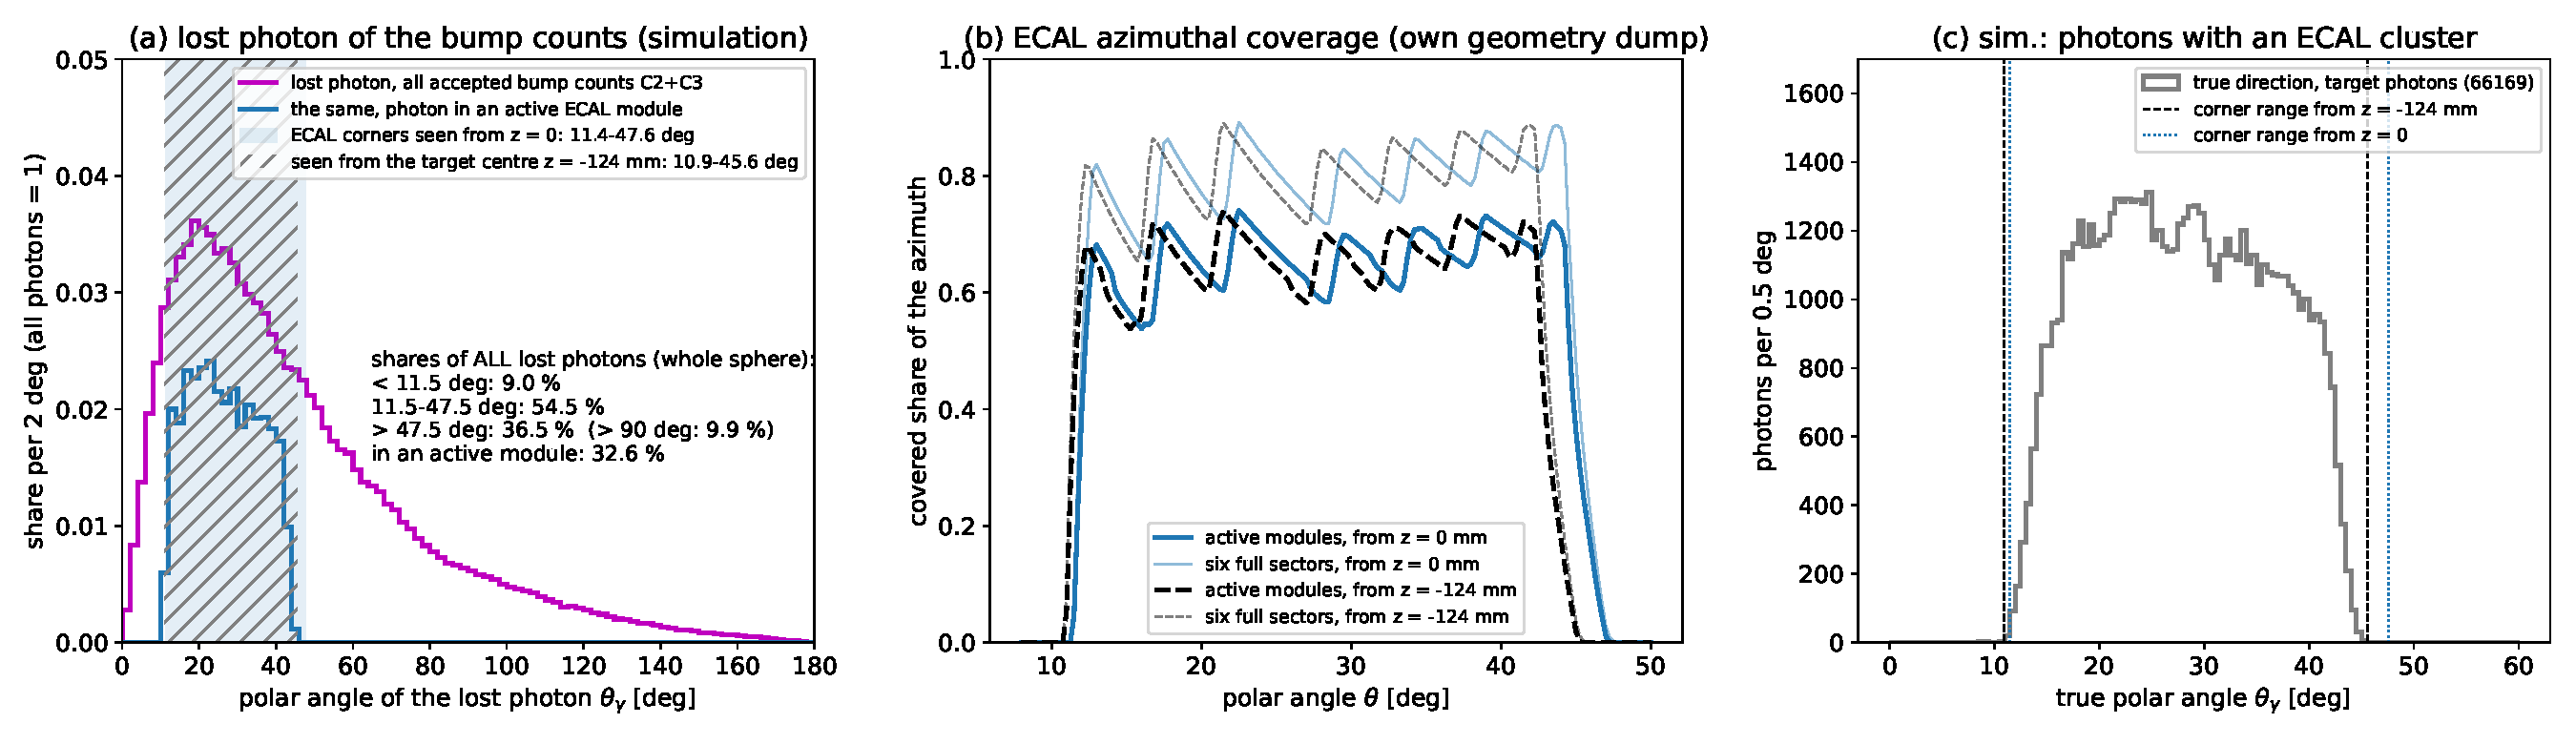
\includegraphics[width=\textwidth]{figs_all/vecalacc_theta_cnt.pdf}
\caption{\textbf{What it shows: one third of the lost bump photons hit an active ECAL module; over the whole sphere 9\,\% fly below the ECAL, 55\,\%
into its polar band and 37\,\% above it (10\,\% backward), and the ECAL seen from the target centre ($z=-124$\,mm) covers 10.9--45.6$^\circ$.}
Selection: (a) simulation only: the simulated bump classes C2+C3 ($\eta\to\pipi\piz$, $\piz\to\ee\gamma$ or one \piz photon converted, the other photon lost; standard set, mode A, $w\times$V3, expected raw counts at 6079.2\,\nbinv) that pass the base cuts ``pre'' (PT3 trigger; event vertex in the target region, $\vz>-160$\,mm; START-free \betanew identification, pions within 3$\sigma$, leptons within 5$\sigma$ with a RICH ring; energy-loss-corrected momenta of all four tracks; all stored combinations of an event, isBest $\ge0$; no condition on the pions in the event-vertex fit); the verifier's own selection and SMASH $\eta$ density; (b) no event selection (geometry and module status only); (c) no event selection: every simulated photon created near the target (within 10\,mm of the beam axis and 40\,mm of $z=-124$\,mm) that made a neutral ECAL candidate, in all events of the standard-set PAT file.
Verification figure (vecalacc). (a) Polar angle of the lost photon of the accepted bump combinations C2+C3 (``pre'', own conditional completion, own SMASH
sample), all (magenta) and in an active module (blue); shaded: module corners seen from $z=0$; hatched: from the target centre. (b) Covered share of
the azimuth against the polar angle, active modules and six full sectors, from $z=0$ and $z=-124$\,mm. (c) True polar angle of target photons that
made an ECAL cluster (all standard-set events); dashed / dotted: the corner range from $z=-124$\,mm and from $z=0$.}
\label{fig:vecalacc}
\end{figure}

%======================================================================
\section{A flexible SMASH description}
\label{sec:flex}
%======================================================================
\inshort{SMASH is used as a set of components, each with its own free scale, and every scale is documented with what fixes it. The $\eta$ signal
classes C2, C4 and C5 share one scale, $0.46\pm0.06$ of SMASH ($0.57\pm0.07$ after the template-noise correction); the direct decays give
$0.63\pm0.12\pm{\approx}0.1$; the non-$\eta$ background above the peak is 10--30\,\% above SMASH, but its split between $G_D$, $G_C$ and \Geta is not
determined. The scales depend on the fit method beyond their errors, are dominated by the template noise of the simulation, cannot be carried
above \Mfour$=0.70$\,\GeVcc, and the model is still incomplete ($p<0.001$). They are a documented description, not measurements (D36).}

\subsection{The model and the fit}
\label{sec:flex-model}
\textbf{In plain words.} In every bin $i$ the expected number of counts is
\begin{equation}
\mu_i=\kEtwo\,\mathrm{CB}_i+\sum_t s_t\,T_{t,i},
\label{eq:flex}
\end{equation}
with one free scale $s_t$ per SMASH component $T_t$ (1 $=$ SMASH as is): C2 and C3 (the bump), C4 and C5 (the peak), \Geta (other $\eta$ decays),
$G_D$ (non-$\eta$ Dalitz pair) split into $G_D(\omega/\rho)$ (both pions from one $\omega$ or $\rho^0$) and $G_D$(other), and $G_C$ (non-$\eta$
conversion pair). The CB comes from the like-sign data, with \kEtwo constrained to $1\pm0.05$. The fit uses the 350 bins of Part~III: five
\Mpipi slices, \Mee$\ge10$\,\MeVcc, \Mfour 0.40--0.70\,\GeVcc, S0, isBest $\ge0$.

\textbf{The fit method} is the Part~III quasi-likelihood of WP4/WP5: an iteratively reweighted Poisson fit in which the weight $1/V$ of every bin
contains the BB-lite variance of the raw $\eta$ templates multiplied by the square of their fitted scales, without nuisance parameters. The
$\eta$ templates (C2--C5, \Geta) are raw; the non-$\eta$ templates are smoothed with exp(pol3) per histogram. Errors: stat from the sandwich formula
(event-group covariance, CB replicas, the \kEtwo constraint); MC from 100 refits with the bootstrap replicas of the simulation (smoothing redone);
total $=$ stat $\oplus$ MC. Goodness of fit: the hybrid GLS $\chi^2$ of Part~III (data covariance, BB-lite diagonal of the raw templates, replica
covariance of the smoothed ones). Checks: the histograms reproduce the factory file to $10^{-14}$, and the Part~III fit F-main is reproduced to
$4\times10^{-8}$ (\aEta 0.382284, hybrid GLS 648.4). The verifier rebuilt the fit with its own inputs and its own solver and reproduced every scale
to $10^{-6}$.

\textbf{SMASH as is} (no parameter fitted; Fig.~\ref{fig:flex-asis}): $(N-\mathrm{CB})$/SMASH is 1.12 over the fit range, 0.85 in the bump window B,
1.05 in the peak window P and 1.20 in CR-U (0.565--0.70\,\GeVcc); hybrid GLS $\chi^2=1789$, Pearson 8398 for 350 bins. The non-$\eta$ background
dominates: $G_D$ 66\,\% of SMASH in the fit range, $G_C$ 16\,\%, \Geta 8\,\%; C2 24\,243, C3 5618, C4 1341, C5 5192 counts.

\begin{figure}[!htb]
\centering
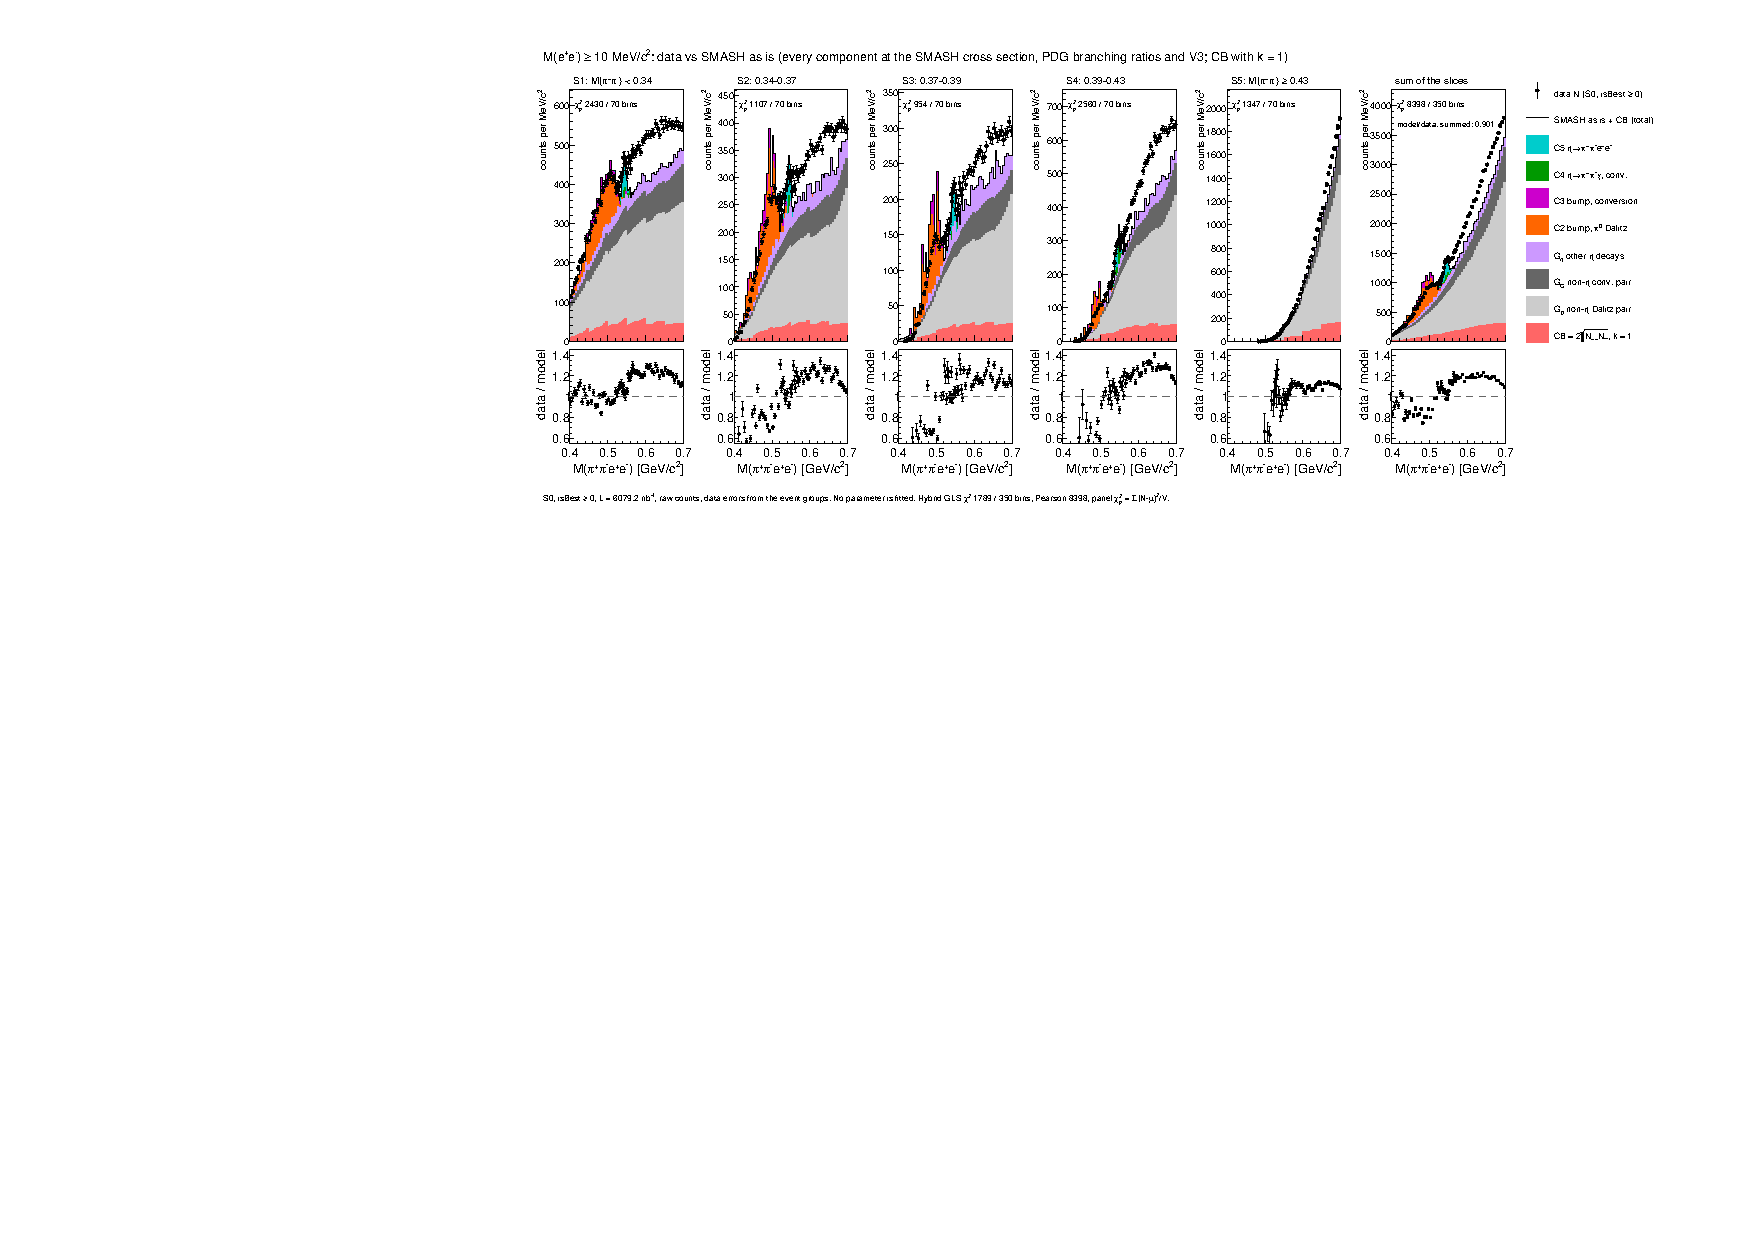
\includegraphics[width=\textwidth]{figs_all/flex_spectra_asis_v2_cnt.pdf}
\caption{\textbf{What it shows: SMASH as is puts too much in the bump (slices S2--S4) and too little above the peak (every \Mpipi slice).}
Selection: data at $L=6079.2\,\nbinv$ with the nominal cuts S0 (PT3 trigger; event vertex in the target region, $\vz>-160$\,mm; START-free \betanew identification, pions within 3$\sigma$, leptons within 5$\sigma$ with a RICH ring; energy-loss-corrected momenta of all four tracks; both pions used in the event-vertex fit; all stored combinations of an event, isBest $\ge0$); \Mee$\ge10$\,\MeVcc; five \Mpipi slices (below 0.34, 0.34--0.37, 0.37--0.39, 0.39--0.43, from 0.43\,\GeVcc); \Mfour 0.40--0.70\,\GeVcc, 70 bins per slice (5\,\MeVcc; 2.5\,\MeVcc in 0.52--0.57), 350 bins; CB $=2\sqrt{N_{++}N_{--}}$ of the like-sign data with the same cuts (10\,\MeVcc cells of \Mfour, $k=1$, shared over the \Mpipi and \Mee cells by the like-sign share of each 50\,\MeVcc band); SMASH (standard, lepton and $\eta$ sets, 221.05\,\nbinv each, every count from one set only, mode A; every channel at its SMASH cross section $\times$ PDG BR $\times$ the $\eta$-decay weights V3; simulated \Mfour$\times0.99615$, \Mpipi$\times0.9952$), with the same cuts; no parameter fitted.
Data $N$ (black points; event-group errors), S0, isBest $\ge0$, $L=6079.2\,\nbinv$, raw counts per \MeVcc, \Mee$\ge10$\,\MeVcc, in the five
\Mpipi slices and summed (right). Stack, every component at its SMASH cross section $\times$ PDG BR $\times$ V3: CB $=2\sqrt{N_{++}N_{--}}$ with $k=1$
(red), $G_D$ (light grey), $G_C$ (dark grey), \Geta (violet), C2 (orange), C3 (magenta), C4 (green), C5 (cyan); black line: the total. Lower row:
data/model. Panel $\chi^2_P=\sum(N-\mu)^2/V$; their sum is the Pearson value 8398 (hybrid GLS 1789). No parameter is fitted.}
\label{fig:flex-asis}
\end{figure}

\subsection{Rules of the model choice (D36)}
\label{sec:flex-rules}
The scales were added step by step with the Part~III rule D11: a group of terms is added only if the hybrid GLS $\chi^2$ drops by more than 4;
physics first (the $\omega/\rho^0$ split of $G_D$, then of $G_C$), then shape freedom (a common tilt $1+bx$, per-slice tilts $1+b_jx$ of $G_D$ and
$G_C$, $x=(\Mfour-0.55)/0.1$). Table~\ref{tab:flex-grid} lists every model.

\begin{table}[H]
\centering
\caption{\textbf{What it shows: the model ladder; more freedom lowers the hybrid GLS $\chi^2$, but this statistic cannot rank nested models (see
text), so the choice of F8 is a convention.} 350 bins; ``free'' counts the scales, tilts and \kEtwo. Lower part: tied versions of F8 by the
verifier (fewer free scales, yet lower values).}
\label{tab:flex-grid}
\footnotesize
\begin{tabularx}{\textwidth}{@{}>{\raggedright\arraybackslash}p{4.3cm} r r r L@{}}
\toprule
model & free & Pearson & hybrid GLS & content \\
\midrule
ASIS & 0 & 8398 & 1789 & SMASH as is (no fit) \\
P3 & 12 & 1159 & 648 & Part~III F-main, reproduced \\
F7 & 8 & 1026 & 628 & 7 scales (C2, C3, C4, C5, \Geta, $G_D$, $G_C$) \\
F7b / F7bj & 9 / 13 & 1033 / 1073 & 628 / 603 & F7 + common tilt / + per-slice tilts (\textbf{alternative F7bj}) \\
F8 & 9 & 1119 & 604 & 8 scales, $G_D$ split into $\omega/\rho^0$ pions and the rest (\textbf{nominal}) \\
F8b / F8bj & 10 / 14 & 1159 / 1065 & 596 / 561 & F8 + common tilt / + per-slice tilts \\
F9, F9b, F9bj & 10, 11, 15 & 1115, 1158, 1000 & 593, 560, 480 & 9 scales ($G_C$ split too), no tilt / common / per slice \\
F7cj & 13 & 1087 & 634 & Part~III background $c_j(1+bx)[G_D+s_{GC}G_C]$, free $\eta$ classes \\
\midrule
F8, all five $\eta$ scales tied & 5 & -- & 574 & 4 parameters fewer than F8 \\
F8, \Geta $=$ C2 / C5 $=$ C2 / $G_D(\omega/\rho)=G_D$(other) & 8 & -- & 551 / 590 / 593 & \\
F8, C2 $=$ C3 $=$ C4 $=$ C5 / \Geta $=$ C5 / \Geta $=1$ & 6 / 8 / 8 & -- & 621 / 641 / 614 & \\
\bottomrule
\end{tabularx}
\end{table}

\textbf{What happened.} The plain D11 rule ends at F9bj, with $s_{GC}(\omega/\rho)=-5.0\pm2.7$ (unphysical) and $s_{GD}(\omega/\rho)=0.70\pm0.97$:
the splits and the tilts are degenerate. After seeing this, three admissibility conditions were added: (b) a new scale must be determined to better
than 50\,\%; (c) no scale determined to better than 50\,\% may become worse than 50\,\%; (d) every scale stays above $-2\sigma_{\mathrm{tot}}$. With
them: F7 $\to$ F8 ($\Delta\chi^2=24.3$, added); F8 $\to$ F9 (10.9, rejected: $s_{GC}(\omega/\rho)$ $\pm541$\,\%); F8 $\to$ F8b (7.5, rejected:
$s_{GD}(\omega/\rho)$ from 35 to 256\,\%); F8 $\to$ F8bj (42.6, rejected: 248\,\%). \textbf{Nominal: F8.} In the order tilts first, F7 $\to$ F7bj (24.9,
added) $\to$ F8bj (rejected): \textbf{alternative: F7bj} (Fig.~\ref{fig:flex-alt}).

\textbf{What this choice is worth.} The verifier showed that the hybrid GLS $\chi^2$ cannot compare nested models: its covariance grows with the
fitted scales, so a model with \emph{fewer} free scales can reach a \emph{lower} value (all five $\eta$ scales tied: 574 instead of 604; \Geta tied to
C2: 551), and minimising the statistic directly gives 416 at the absurd point $s_{GC}=16$, $s_{GD}(\omega/\rho)=-5.5$. The ladder steps
($+24.3$, $+10.9$, $+7.5$, $+24.9$) are therefore not significance statements; ``F8 describes the data better than Part~III (604 against 648)''
does not hold as a comparison; and the need for the $G_D$ split is not established (tying the two parts gives 593; most of the gain of F7 $\to$ F8
comes from smoothing the two parts separately). The goodness of fit of F8 itself stays valid, because its pseudo-data use the same statistic
(\S\ref{sec:flex-gof}).

\notebox{\textbf{D36 (decision of the lead analysis, approved by the analyst on 15 November 2026).} The flexible model F8 was chosen with the three conditions
(b)--(d), added after the first ladder result (F9bj) had been seen; F7bj and the tied fits are the model alternatives. The per-channel scales are a
documented description of the data in \Mfour 0.40--0.70\,\GeVcc, each with what fixes it (Table~\ref{tab:flex-scales}), and \emph{not}
measurements; no headline number of this report is taken from them.}

\begin{figure}[!htb]
\centering
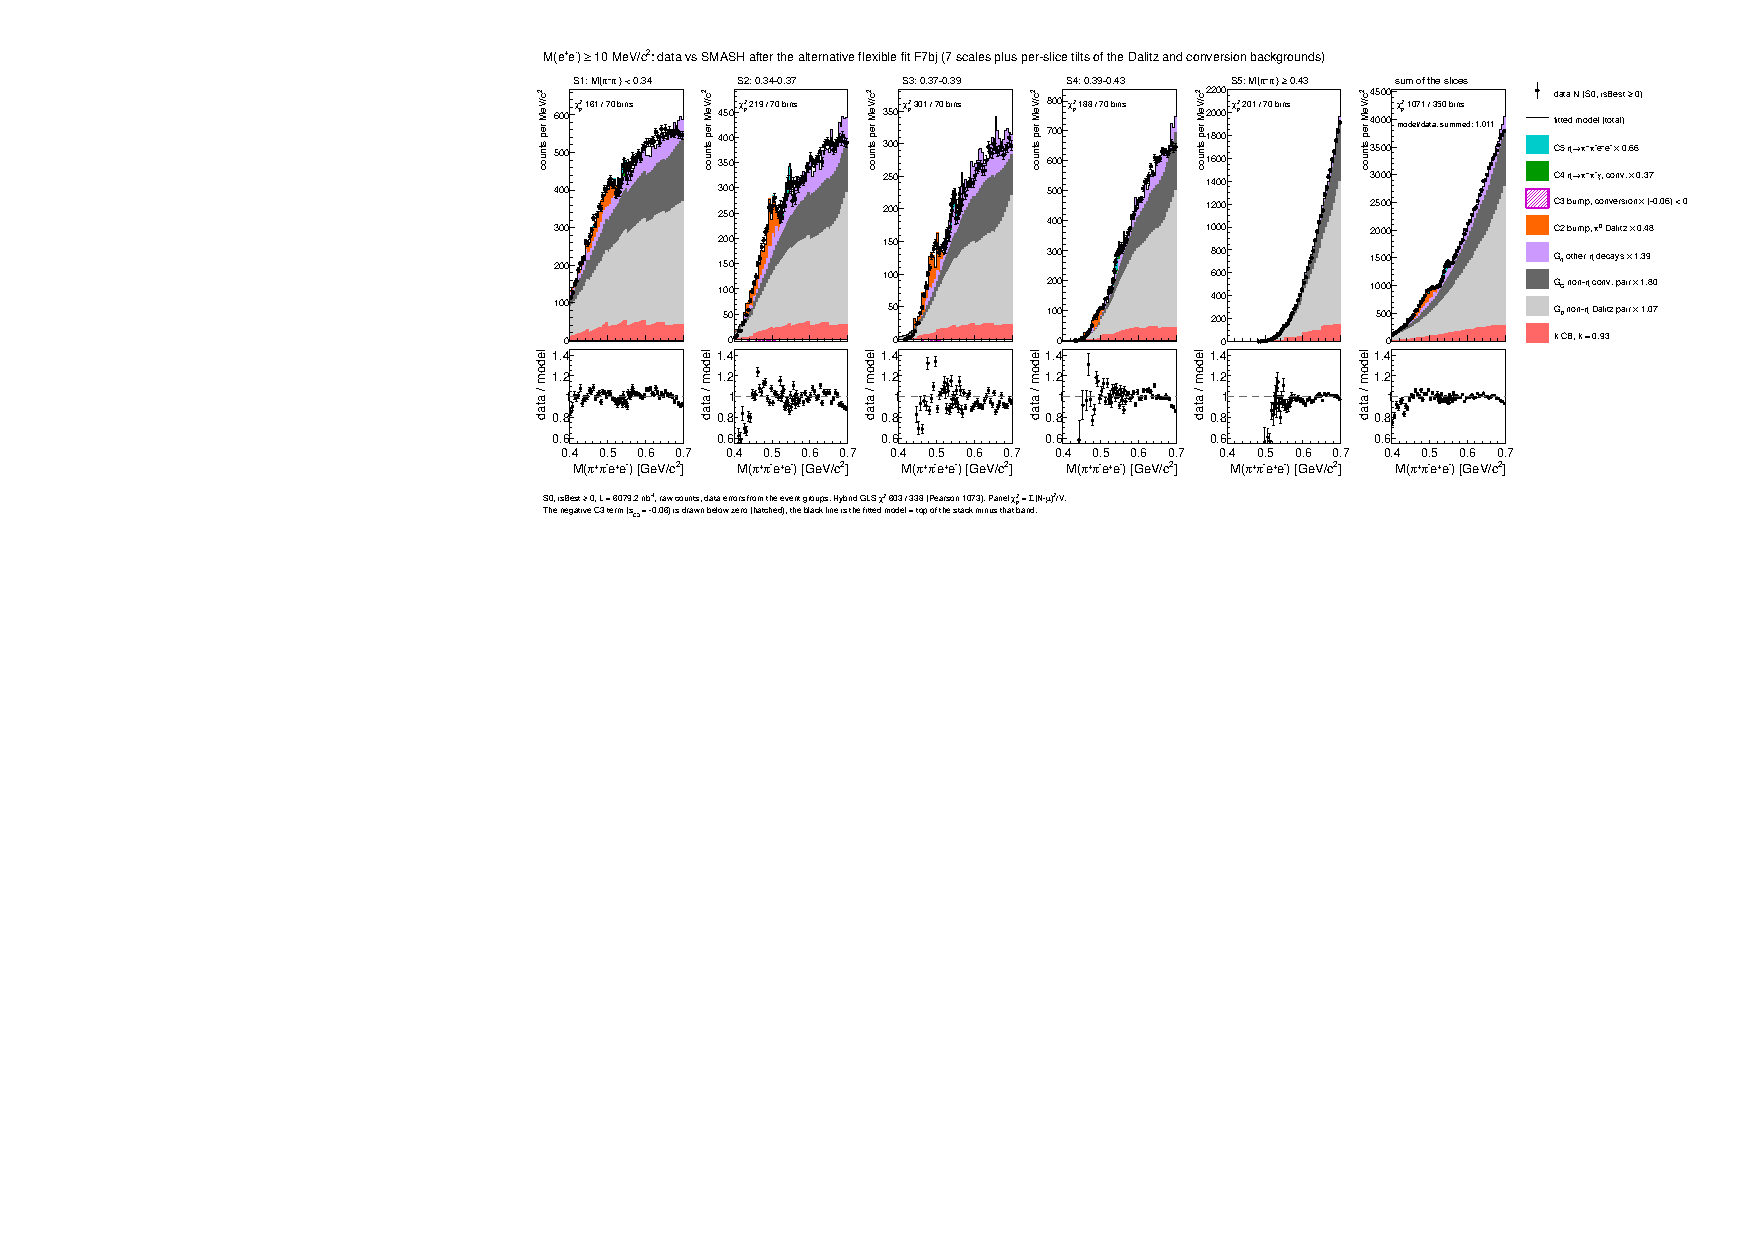
\includegraphics[width=\textwidth]{figs_all/flex_spectra_alt_v2_cnt.pdf}
\caption{\textbf{What it shows: the alternative flexible fit F7bj (seven scales plus per-slice tilts of $G_D$ and $G_C$) describes the data as F8 does
and gives similar signal scales.}
Selection: as the nominal flexible fit, data at $L=6079.2\,\nbinv$ with the nominal cuts S0 (PT3 trigger; event vertex in the target region, $\vz>-160$\,mm; START-free \betanew identification, pions within 3$\sigma$, leptons within 5$\sigma$ with a RICH ring; energy-loss-corrected momenta of all four tracks; both pions used in the event-vertex fit; all stored combinations of an event, isBest $\ge0$); \Mee$\ge10$\,\MeVcc; five \Mpipi slices (below 0.34, 0.34--0.37, 0.37--0.39, 0.39--0.43, from 0.43\,\GeVcc); \Mfour 0.40--0.70\,\GeVcc, 70 bins per slice (5\,\MeVcc; 2.5\,\MeVcc in 0.52--0.57), 350 bins; CB $=2\sqrt{N_{++}N_{--}}$ of the like-sign data with the same cuts (10\,\MeVcc cells of \Mfour, shared over the \Mpipi and \Mee cells by the like-sign share of each 50\,\MeVcc band), times a factor $k$ fitted within $1\pm0.05$; SMASH (standard, lepton and $\eta$ sets, 221.05\,\nbinv each, every count from one set only, mode A; every channel at its SMASH cross section $\times$ PDG BR $\times$ the $\eta$-decay weights V3; simulated \Mfour$\times0.99615$, \Mpipi$\times0.9952$), with the same cuts.
As Fig.~\ref{fig:res-flexfit}: data $N$ (black), stack $k\,$CB (red, $k=0.93$), $G_D$ (light grey, $\times1.07$), $G_C$ (dark grey, $\times1.80$),
\Geta (violet, $\times1.39$), C2 (orange, $\times0.48$), C4 (green, $\times0.37$), C5 (cyan, $\times0.66$); the negative C3 ($s_{\mathrm{C3}}=-0.06$) is
hatched below zero, and the black line is the fitted model. Panel $\chi^2_P=\sum(N-\mu)^2/V$; hybrid GLS 603/338 (Pearson 1073); summed
model/data 1.011.}
\label{fig:flex-alt}
\end{figure}

\subsection{The scales and what fixes them}
\label{sec:flex-scales}

\begin{table}[!htb]
\centering
\caption{\textbf{What it shows: every scale of the nominal flexible fit F8, what fixes it, and how far it can be trusted.} Value $\pm$ stat $\pm$ MC;
$\sigma/s=$ total relative error; ``fixed by'': share of the Fisher information by \Mfour region (B bump window, P peak window, CR-U 0.565--0.70)
and slice; ``degenerate'': $|\rho|>0.8$ (stat $+$ MC); bias test: bias of the realistic fit on pseudo-data with the fitted scales as truth (RF) and
its verdict; fit method: range of the scale when the weight $\lambda$ of the template noise in the fit weights runs from 0.5 to 1.5 (verifier);
reading: what the scale can be used for. Fig.~\ref{fig:res-flex} shows the same.}
\label{tab:flex-scales}
\footnotesize
\setlength{\tabcolsep}{2.5pt}
\begin{tabularx}{\textwidth}{@{}l l r >{\raggedright\arraybackslash}p{2.35cm} l >{\raggedright\arraybackslash}p{1.6cm} l L@{}}
\toprule
scale & value $\pm$ stat $\pm$ MC & $\sigma/s$ & fixed by & degenerate & bias test & $\lambda$ 0.5--1.5 & reading \\
\midrule
C2 & $0.412\pm0.021\pm0.065$ & 17\,\% & B 82\,\%, $<0.455$ 17\,\% & -- & $-20$\,\%, fail & 0.37--0.41 & one $\eta$ scale with C4, C5; attenuated \\
C3 & $-0.087\pm0.067\pm0.228$ & 273\,\% & B 74\,\%, $<0.455$ 25\,\% & -- & $+1.6\sigma$, fail & 0.14 to $-0.13$ & not determined (needs \Mee$<10$) \\
C4 & $0.335\pm0.158\pm0.155$ & 66\,\% & P 75\,\%, 0.5225--0.534 20\,\% & -- & $-58$\,\%, fail & 0.35 & weak; one $\eta$ scale with C2, C5 \\
C5 & $0.626\pm0.064\pm0.099$ & 19\,\% & P 96\,\% & -- & $+1$\,\%, pass & 0.57--0.67 & determined; $\pm{\approx}0.1$ model/method \\
\Geta & $2.102\pm0.072\pm0.584$ & 28\,\% & CR-U 76\,\% (S1 39\,\%) & $G_C$ & $-15$\,\%, fail & 1.52--2.96 & not determined \\
$G_D(\omega/\rho)$ & $0.788\pm0.050\pm0.275$ & 35\,\% & CR-U 98.5\,\% (S5 76\,\%) & $G_C$ & $-15$\,\%, fail & 0.58--1.10 & not determined \\
$G_D$(other) & $1.109\pm0.030\pm0.107$ & 10\,\% & CR-U 77\,\% (S5 49\,\%) & $G_C$ & $+4$\,\%, marginal & 1.06--1.18 & close to SMASH (0.89--1.27 in all fits) \\
$G_C$ & $1.596\pm0.122\pm0.674$ & 43\,\% & CR-U 85\,\% (S5 45\,\%) & \Geta, $G_D$ & $+5$\,\%, pass & 2.11--0.83 & not determined \\
\kEtwo & $0.907\pm0.045\pm0.043$ & 7\,\% & constraint $1\pm0.05$ & -- & $-1$\,\%, pass & 0.90--0.92 & nuisance; $1.9\sigma$ below 1 \\
\bottomrule
\end{tabularx}
\end{table}

\textbf{What each scale does} (counts in the windows, SMASH $\to$ F8): C2 in B 19\,750 $\to$ 8129; C3 in B 4955 $\to$ $-432$; C4 in P 914 $\to$ 306; C5 in
P 4300 $\to$ 2693; \Geta in B / P / CR-U 3318 $\to$ 6974, 2149 $\to$ 4518, 23\,088 $\to$ 48\,528; $G_D(\omega/\rho)$ in CR-U 42\,265 $\to$ 33\,315;
$G_D$(other) in B / P / CR-U 21\,990 $\to$ 24\,376, 13\,222 $\to$ 14\,657, 155\,304 $\to$ 172\,156; $G_C$ in B / P / CR-U 4866 $\to$ 7767, 3243 $\to$ 5176,
49\,258 $\to$ 78\,619; $k\,$CB in B 5668 $\to$ 5141. \Geta, both parts of $G_D$ and $G_C$ are all fixed by the same CR-U bins; that is why they are
degenerate (Fig.~\ref{fig:flex-corr}): $G_C$ is anti-correlated with \Geta ($-0.88$) and with both parts of $G_D$ ($-0.82$, $-0.85$); in F7bj, $G_D$
and $G_C$ reach $-0.94$.

\textbf{Ratios} (stat, MC): $s_{\mathrm{C5}}/s_{\mathrm{C2}}=1.52\pm0.16\pm0.49$; $s_{\mathrm{C4}}/s_{\mathrm{C2}}=0.81\pm0.39\pm0.54$;
$s_{GC}/s_{GD}(\mathrm{other})=1.44\pm0.14\pm0.78$; $s_{GD}(\omega/\rho)/s_{GD}(\mathrm{other})=0.71\pm0.05\pm0.23$. Content-weighted means over the
fit bins: bump C2+C3 $0.318\pm0.043$, peak C4+C5 $0.567\pm0.086$.

\begin{figure}[!htb]
\centering
\begin{minipage}[t]{0.49\textwidth}\centering
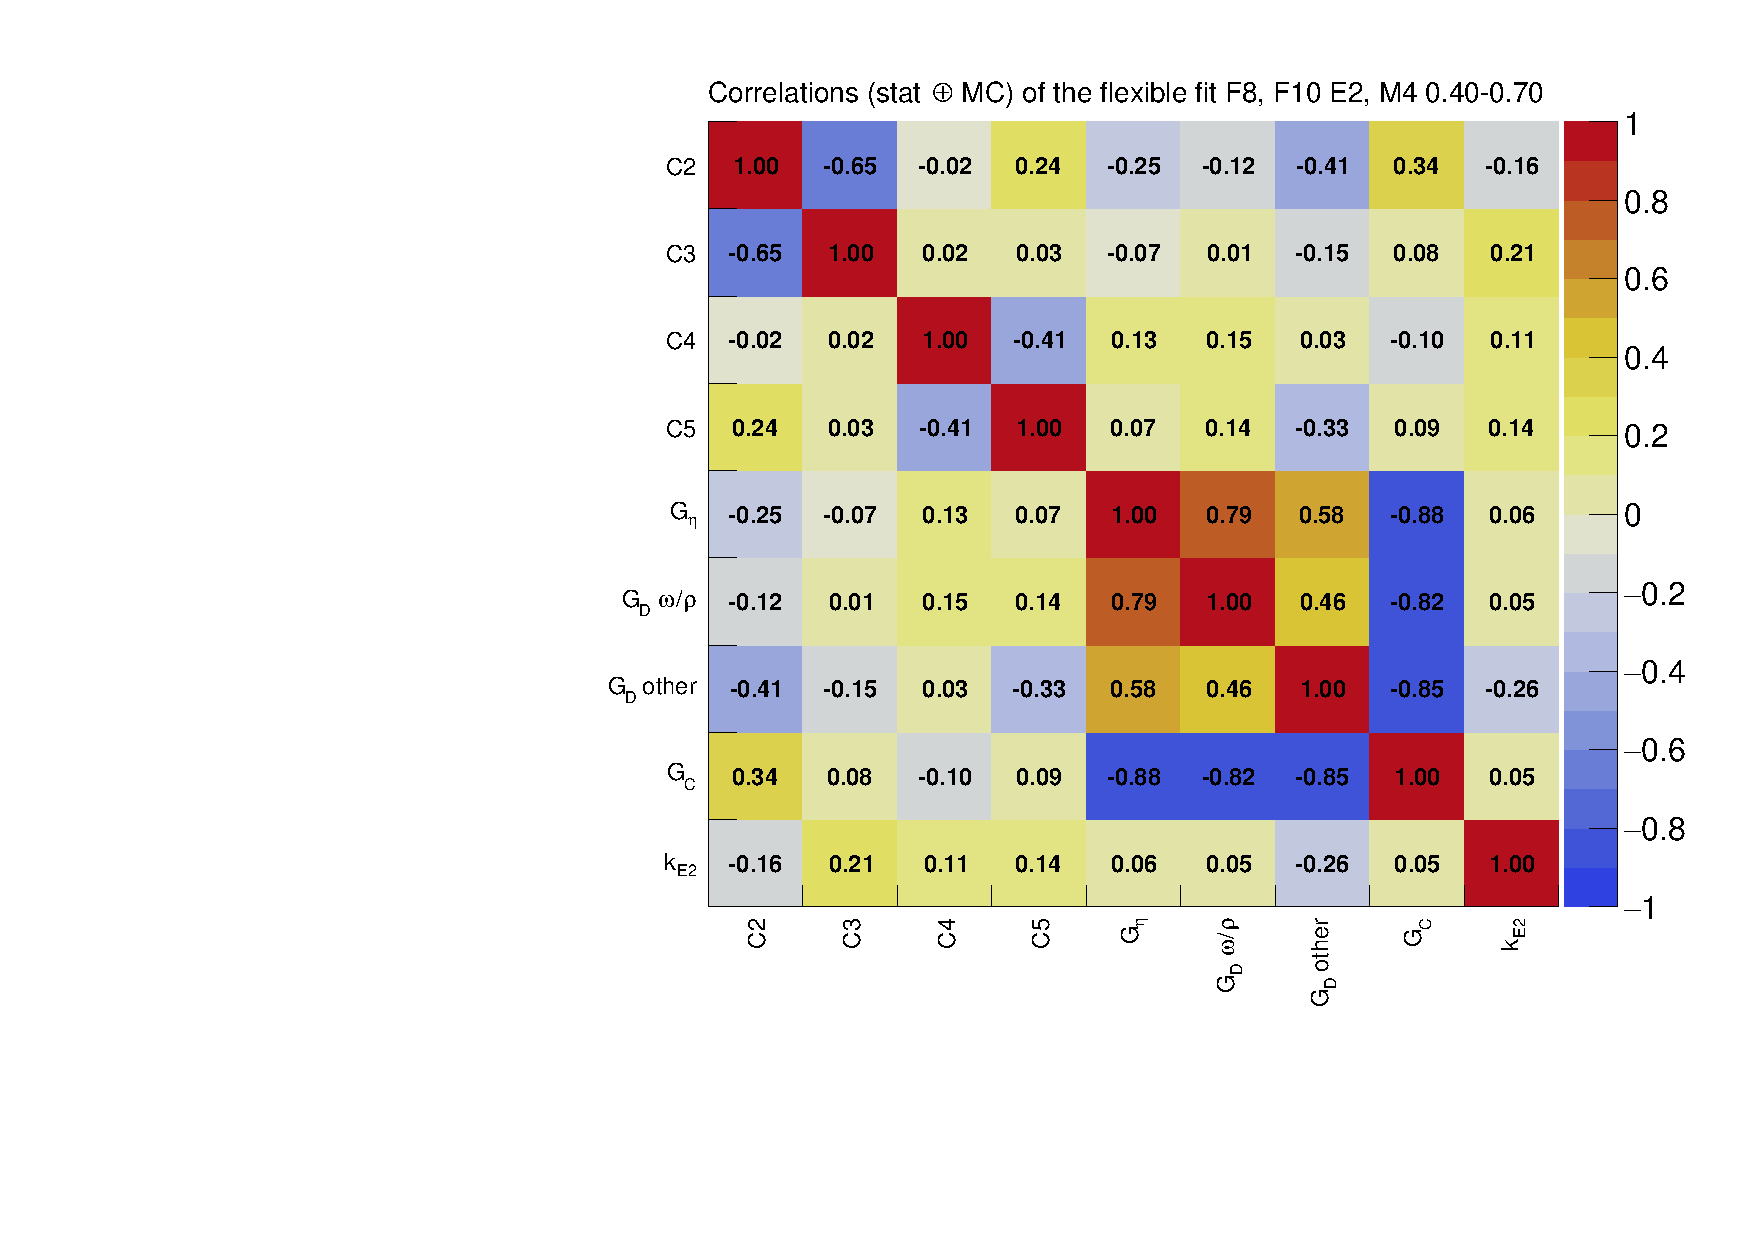
\includegraphics[width=\textwidth]{figs_all/flex_corr_v2.pdf}\\[-0.3em]{\small (a) F8}
\end{minipage}\hfill
\begin{minipage}[t]{0.49\textwidth}\centering
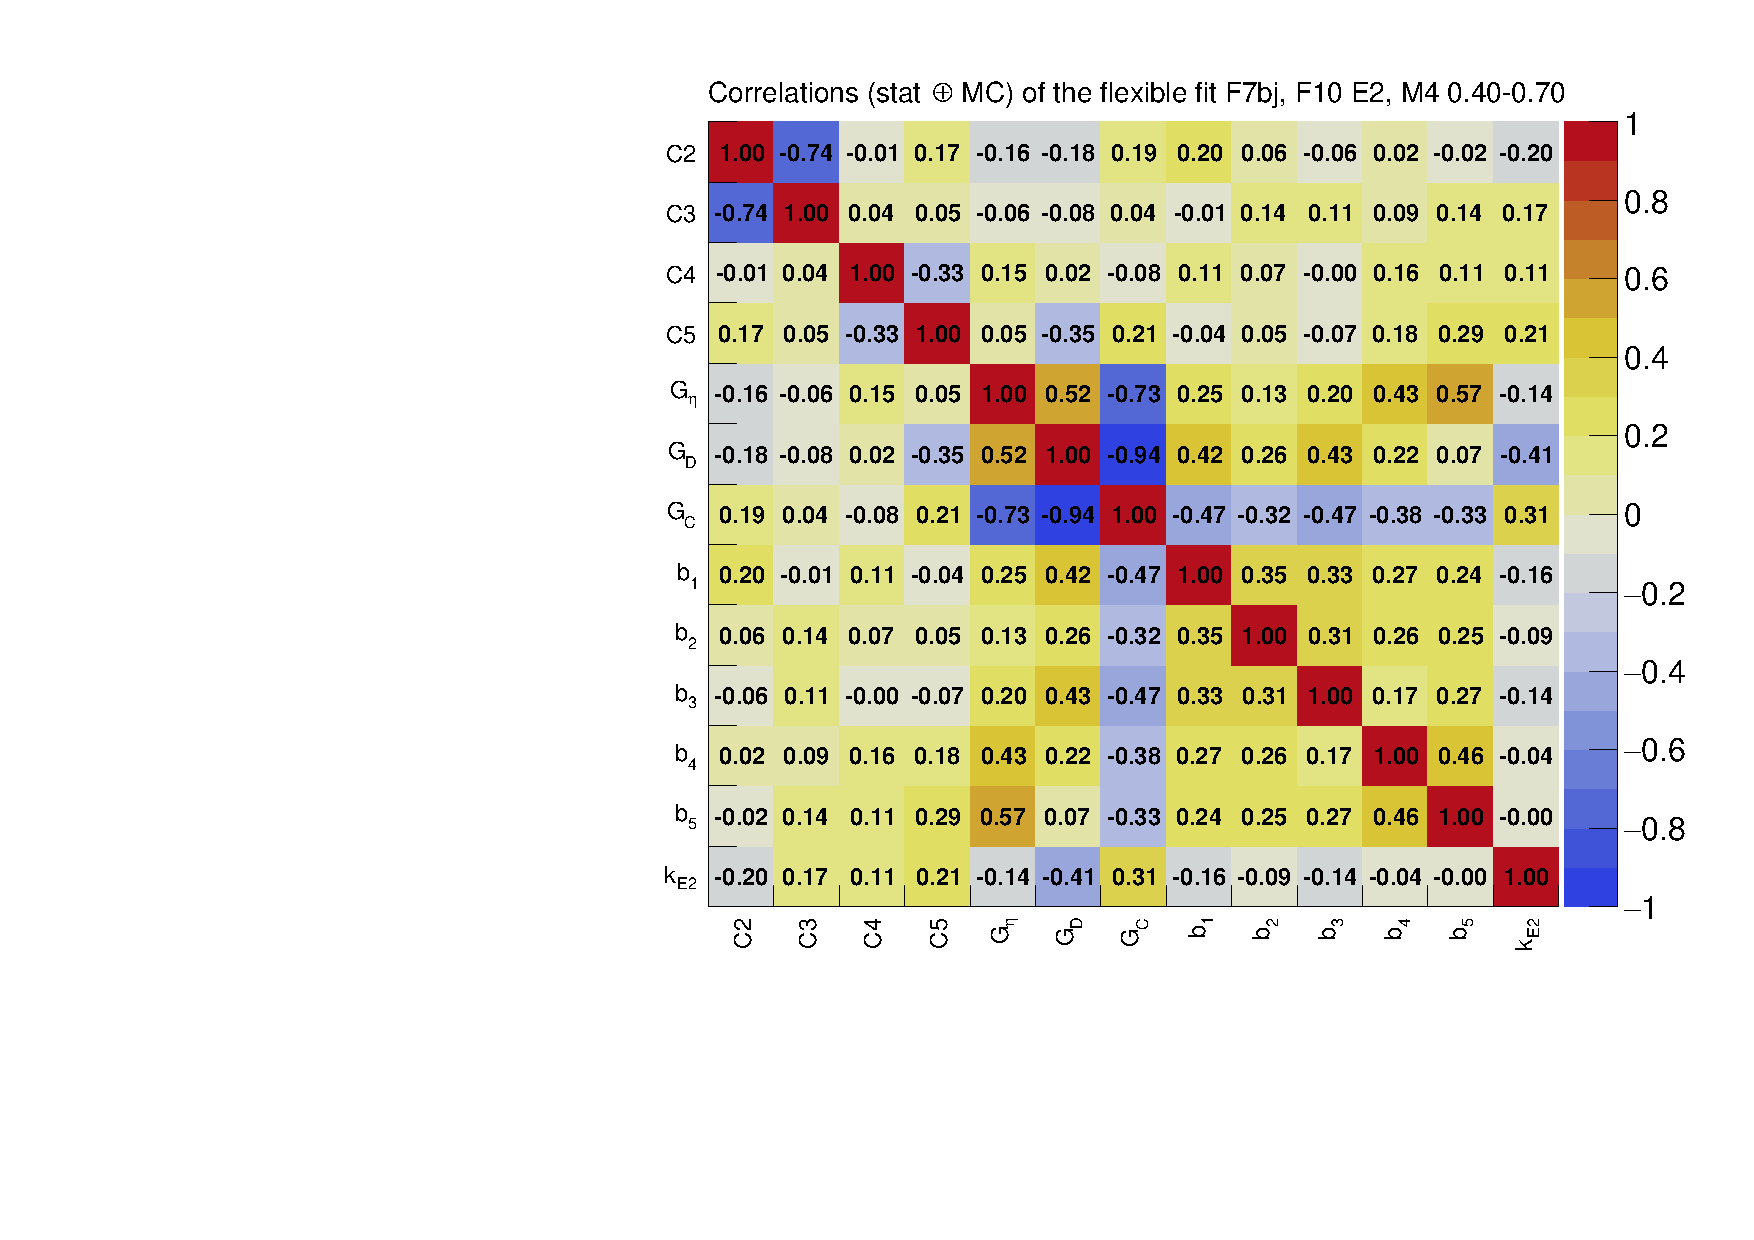
\includegraphics[width=\textwidth]{figs_all/flex_corr_alt_v2.pdf}\\[-0.3em]{\small (b) F7bj}
\end{minipage}
\caption{\textbf{What it shows: the background scales fixed above the peak (\Geta, $G_D$, $G_C$) are strongly anti-correlated, so their split is not
determined; the $\eta$ signal scales are nearly independent of them.}
Selection: the fits of Figs.~\ref{fig:res-flexfit} and \ref{fig:flex-alt}: data at $L=6079.2\,\nbinv$ with the nominal cuts S0 (PT3 trigger; event vertex in the target region, $\vz>-160$\,mm; START-free \betanew identification, pions within 3$\sigma$, leptons within 5$\sigma$ with a RICH ring; energy-loss-corrected momenta of all four tracks; both pions used in the event-vertex fit; all stored combinations of an event, isBest $\ge0$); \Mee$\ge10$\,\MeVcc; five \Mpipi slices (below 0.34, 0.34--0.37, 0.37--0.39, 0.39--0.43, from 0.43\,\GeVcc); \Mfour 0.40--0.70\,\GeVcc, 70 bins per slice (5\,\MeVcc; 2.5\,\MeVcc in 0.52--0.57), 350 bins; CB $=2\sqrt{N_{++}N_{--}}$ of the like-sign data with the same cuts (10\,\MeVcc cells of \Mfour, shared over the \Mpipi and \Mee cells by the like-sign share of each 50\,\MeVcc band), times a factor $k$ fitted within $1\pm0.05$; SMASH (standard, lepton and $\eta$ sets, 221.05\,\nbinv each, every count from one set only, mode A; every channel at its SMASH cross section $\times$ PDG BR $\times$ the $\eta$-decay weights V3; simulated \Mfour$\times0.99615$, \Mpipi$\times0.9952$), with the same cuts.
Correlation matrices (stat $\oplus$ MC) of (a) the nominal fit F8 and (b) the alternative F7bj ($b_1$--$b_5$: the per-slice tilts); F10 layout,
\Mee$\ge10$\,\MeVcc, \Mfour 0.40--0.70\,\GeVcc.}
\label{fig:flex-corr}
\end{figure}

\subsection{What is robust and what is not}
\label{sec:flex-robust}
The verifier tried to refute every plain-words conclusion with tied fits, Wald tests, a scan of the fit weights and two estimators.
\textbf{Robust:}
\begin{itemize}\setlength{\itemsep}{1pt}
\item \textbf{One $\eta$ scale for C2, C4 and C5:} the Wald test with the stat $+$ MC covariance gives a common $0.456\pm0.058$ ($\chi^2=3.2/2$, $p=0.21$);
      after the attenuation correction of the pseudo-data test ($\times1/0.797$, $\times1/0.408$, $\times1/1.01$) $0.571\pm0.071$ ($\chi^2=1.4/2$, $p=0.51$);
      the tied fit C2 $=$ C4 $=$ C5 gives 0.456 without loss. Adding C3 ($-0.09$, undetermined in E2) spoils it ($\chi^2=12.5/3$, $p=0.006$),
      for no physical reason. \Geta is an $\eta$ channel too, but it is not determined (below), so it is left out.
\item \textbf{C5/C2 agrees with the PDG ratio within 1--2$\sigma$}: 1.52 $\pm$ 0.52 in F8 (1.0$\sigma$; Part~III $\rhod=1.32\pm0.25$), $1.98\pm0.48$ in
      the variant with the class \Mee$<10$\,\MeVcc (2.0$\sigma$), 1.79 with E2 split at 20\,\MeVcc; the attenuation of C2 lowers these by a factor 0.8.
\item \textbf{The direct decays:} $s_{\mathrm{C5}}=0.63\pm0.12$ (stat $\oplus$ MC) $\pm$ about 0.1 (model and fit method): the variants of
      0.40--0.70\,\GeVcc span 0.44--0.94, the fit weights 0.48--0.69. SMASH $\times$ PDG BR is 1.4--2 times too high for C5. It passes the bias test
      with the fitted scales as truth ($+1$\,\%), not with SMASH as truth ($+7.0\pm0.8$\,\%, coverage 0.54); and the fitted model overshoots the peak
      window by 5.8\,\% (\S\ref{sec:flex-gof}), where C5 is fixed.
\item \textbf{The non-$\eta$ background above the peak is 10--30\,\% above SMASH.} As is, data/SMASH in CR-U is 1.20 over all components; in F8 the
      fitted non-$\eta$ part ($G_D+G_C$) is 1.15 $\times$ SMASH there, \Geta supplying the rest; over the tied fits 1.11--1.28. $G_D$(other) stays close
      to 1 (0.89--1.27 over all weightings and tied fits).
\item \textbf{The flexible description is incomplete} (\S\ref{sec:flex-gof}).
\end{itemize}
\textbf{Not robust} (not determinations): \Geta $=2.10$ (1.1--3.9 with the fit weights; in Part~III $ag=0.66$, so the ``2.4$\sigma$ difference from
Part~III'' is not robust); $G_C=1.60$ and $G_D(\omega/\rho)=0.79$; C3 $=-0.09$; and the attenuation-corrected C2 of about 0.52 (the same correction
on the $\lambda=0$ fit gives 0.38): the template noise biases C2 low by about 20\,\%, which is not a determination of its true value.

\subsection{Dependence on the fit method}
\label{sec:flex-method}
In the fit weights the variance of a bin is $V=\max(\mu,1)+k^2\,\mathrm{var}(\mathrm{CB})+\lambda\sum_t s_t^2\,\mathrm{var}(T_{t,\mathrm{raw}})$; the last
term makes the weights depend on the scales. $\lambda=1$ is the nominal fit; $\lambda=0$ is the Poisson likelihood with the templates taken as
exact. Same data, same templates:

\begin{table}[H]
\centering
\caption{\textbf{What it shows: the background scales move along their degenerate direction when the template noise gets more or less weight; the
signal scales move less.} F8 scales against $\lambda$, and the missing systematic of each scale (half the spread between $\lambda=0.5$ and 1.5, the
weightings that are still reasonable; over $\lambda=0$--2 the spread is 2--3 times larger). Verifier (\code{vflex_lamscan.json}).}
\label{tab:flex-lambda}
\footnotesize
\begin{tabular}{@{}l r r r r r@{}}
\toprule
scale & $\lambda=0$ & 0.5 & 1 (nominal) & 2 & missing systematic \\
\midrule
C2 & 0.31 & 0.37 & 0.41 & 0.41 & $\pm0.02$ \\
C3 & 0.39 & 0.14 & $-0.09$ & $-0.14$ & -- \\
C5 & 0.48 & 0.57 & 0.63 & 0.69 & $\pm0.05$ \\
\Geta & 1.11 & 1.52 & 2.10 & 3.88 & $\pm0.72$ \\
$G_D(\omega/\rho)$ & 0.46 & 0.58 & 0.79 & 1.45 & $\pm0.26$ \\
$G_D$(other) & 1.06 & 1.06 & 1.11 & 1.27 & $\pm0.06$ \\
$G_C$ & 2.37 & 2.11 & 1.60 & $-0.02$ & $\pm0.64$ \\
\bottomrule
\end{tabular}
\end{table}

\textbf{Is the difference expected?} If the model were right, the fits with $\lambda=0$ and $\lambda=1$ would agree within the spread of 300 pseudo-data
sets (truth $=$ F8): about $\pm0.03$ for C2 and $\pm0.07$ for C5. On the data they differ by $-0.098$ (C2, $z=-4.1$), $+0.474$ (C3, $+6.8$), $-0.144$ (C5,
$-2.3$), $-0.995$ (\Geta, $-5.2$), with $z=-2.2$ for $G_D(\omega/\rho)$ and $+3.0$ for $G_C$; all nine together $\chi^2=164.6/9$, exceeded by none of the
300. This is a second, independent sign that the scaled-SMASH model does not describe the data, and a systematic that the quoted errors do not
contain. A full Barlow--Beeston profile likelihood (Gaussian nuisances for the raw templates) is worse: unbounded it runs away (\Geta 7.1, $G_C$
$-3.0$, C3 $-1.6$, C4 1.75); bounded to [0, 10] it puts $G_C$ and C3 at the bound and gives \Geta 4.5, C4 1.17, C5 0.59, C2 0.50. A caution for
future users: the fit equations also have false solutions with scales running to infinity, where the template variance kills every weight; an
unbounded root finder started at $s=1$ falls into them, the damped Fisher scoring of the package does not.

\begin{figure}[!htb]
\centering
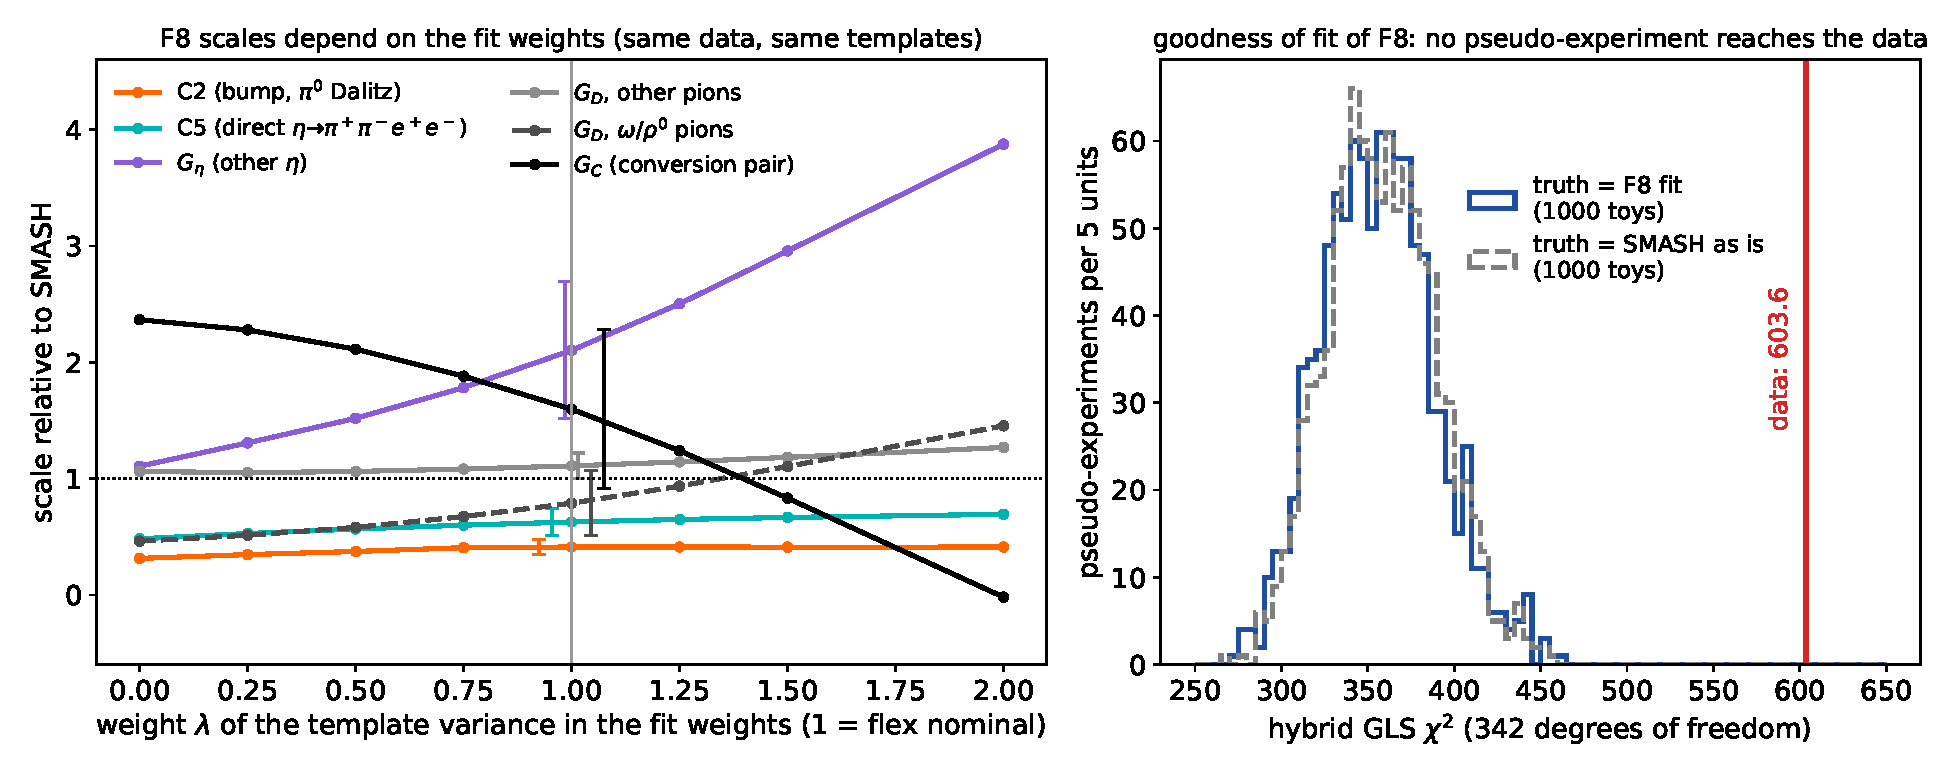
\includegraphics[width=\textwidth]{figs_all/vflex_summary.pdf}
\caption{\textbf{What it shows: the F8 scales depend on how the template noise enters the fit weights, and no pseudo-experiment from a perfect model
reaches the $\chi^2$ of the data.}
Selection: the bins of the nominal flexible fit, data at $L=6079.2\,\nbinv$ with the nominal cuts S0 (PT3 trigger; event vertex in the target region, $\vz>-160$\,mm; START-free \betanew identification, pions within 3$\sigma$, leptons within 5$\sigma$ with a RICH ring; energy-loss-corrected momenta of all four tracks; both pions used in the event-vertex fit; all stored combinations of an event, isBest $\ge0$); \Mee$\ge10$\,\MeVcc; five \Mpipi slices (below 0.34, 0.34--0.37, 0.37--0.39, 0.39--0.43, from 0.43\,\GeVcc); \Mfour 0.40--0.70\,\GeVcc, 70 bins per slice (5\,\MeVcc; 2.5\,\MeVcc in 0.52--0.57), 350 bins; CB $=2\sqrt{N_{++}N_{--}}$ of the like-sign data with the same cuts (10\,\MeVcc cells of \Mfour, shared over the \Mpipi and \Mee cells by the like-sign share of each 50\,\MeVcc band), times a factor $k$ fitted within $1\pm0.05$; SMASH (standard, lepton and $\eta$ sets, 221.05\,\nbinv each, every count from one set only, mode A; every channel at its SMASH cross section $\times$ PDG BR $\times$ the $\eta$-decay weights V3; simulated \Mfour$\times0.99615$, \Mpipi$\times0.9952$), with the same cuts; the pseudo-experiments are drawn in the same 350 bins.
Left: F8 scales of C2 (orange), C5 (cyan), \Geta (violet), $G_D$ other pions (grey), $G_D$ $\omega/\rho^0$ pions (dark grey, dashed) and $G_C$
(black, the darkest of the non-$\eta$ greys) against $\lambda$, the weight of the BB-lite template variance in the fit weights ($\lambda=1$: nominal;
$\lambda=0$: Poisson weights with exact templates); same data and templates for every $\lambda$; bars at $\lambda=1$: the total errors (stat
$\oplus$ MC). Right: hybrid GLS $\chi^2$ of 1000 + 1000 pseudo-experiments with bootstrap-replica templates, truth $=$ the F8 fit (blue) and SMASH
as is (grey dashed); red: the data, 603.6. S0, isBest $\ge0$, \Mee$\ge10$\,\MeVcc, \Mfour 0.40--0.70\,\GeVcc, 350 bins. Verifier vflex.}
\label{fig:flex-method}
\end{figure}

\subsection{Goodness of fit, and where the model misses}
\label{sec:flex-gof}
F8 reaches hybrid GLS $\chi^2=603.6$ for 342 degrees of freedom (Pearson 1119). Pseudo-data from the fitted model with the real template noise give
$356\pm33$ (5 / 50 / 95\,\%: 305 / 356 / 413; largest of 1000: 461), from SMASH as is $359\pm32$ (largest 459): \textbf{none of 2000 reaches the
data, $p<0.001$}; the data lie 7.6 rms above the mean. (The package's own 500 pseudo-data sets gave $p\approx0.002$ through a single outlier set with
$\chi^2=891$ and normal fitted parameters; the verifier's 2000 have none.) \textbf{The fitted model lies above the data}: by 9415 counts ($+2.0$\,\%; data
stat $\pm805$) over the fit range, $+10.2$\,\% below 0.455\,\GeVcc, $-1.0$\,\% in B, $+5.8$\,\% (1697 counts, $\pm186$) in P and $+1.7$\,\% in CR-U, while
pseudo-data from a correct model give $-0.7\pm0.3$\,\% in total and $-0.5\pm1.0$\,\% in P. With $\lambda=0$ the total balances ($+0.01$\,\%), so the
offset is how the misfit shows up with scale-dependent weights. The remaining misfit sits at the lower \Mfour edge of S2 and S3 (data 20--40\,\%
below the model at 0.40--0.47\,\GeVcc) and in $\pm10$\,\% waves in S2--S4 (Fig.~\ref{fig:res-flexfit}); in \Mee (Fig.~\ref{fig:flex-mee}) the fitted
model follows the data in CR-U and in the bump window better than SMASH as is.

\begin{figure}[!htbp]
\centering
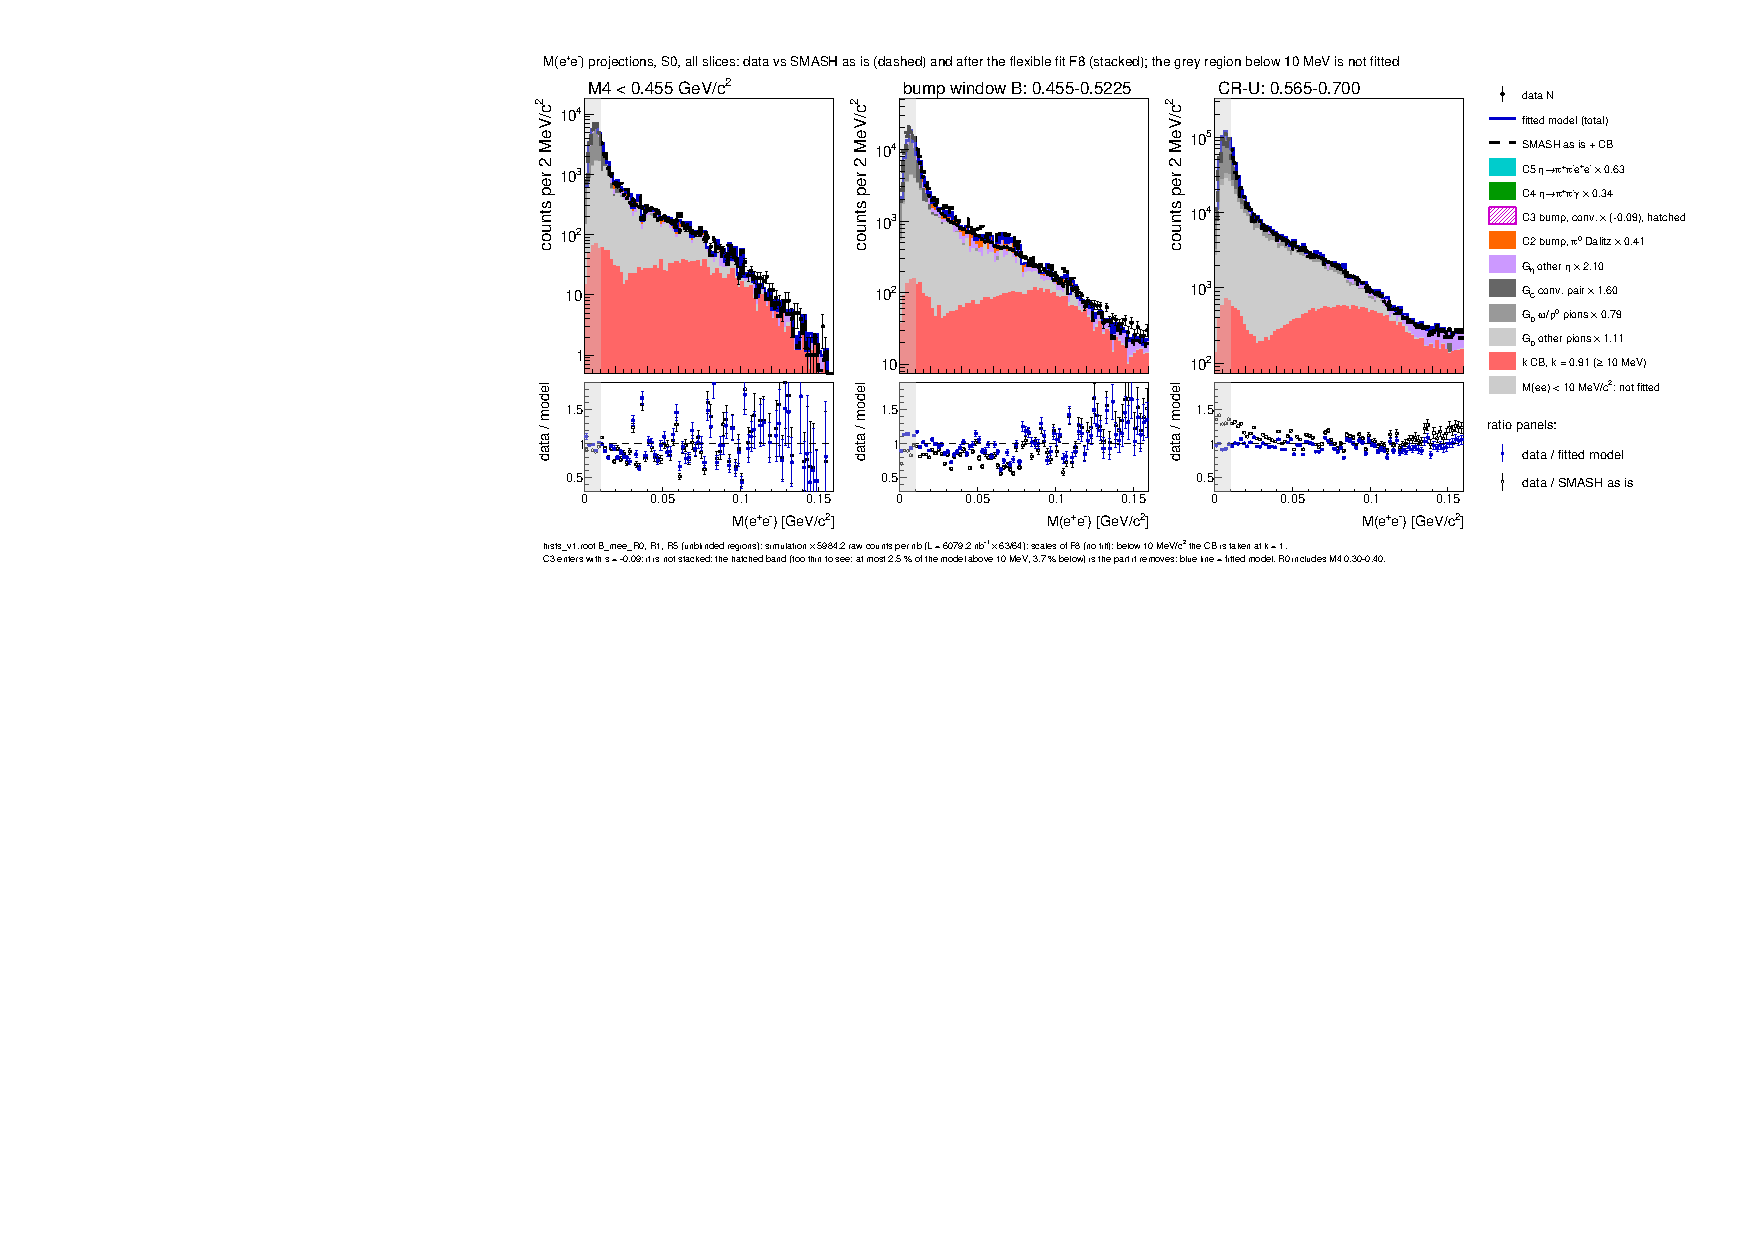
\includegraphics[width=\textwidth]{figs_all/flex_mee_v2_cnt.pdf}
\caption{\textbf{What it shows: in \Mee the fitted model follows the data above the peak and in the bump window better than SMASH as is; below
the bump both overshoot.}
Selection: data at $L=6079.2\,\nbinv$ with the nominal cuts S0 (PT3 trigger; event vertex in the target region, $\vz>-160$\,mm; START-free \betanew identification, pions within 3$\sigma$, leptons within 5$\sigma$ with a RICH ring; energy-loss-corrected momenta of all four tracks; both pions used in the event-vertex fit; all stored combinations of an event, isBest $\ge0$), all \Mpipi; \Mee in 2\,\MeVcc bins, in three \Mfour regions: below 0.455\,\GeVcc (left), the bump window 0.4550--0.5225\,\GeVcc (middle) and 0.565--0.70\,\GeVcc (right); CB $=2\sqrt{N_{++}N_{--}}$ from the like-sign data with the same cuts (10\,\MeVcc cells of \Mfour) for each region, shared over the \Mee bins by the like-sign share of each bin, times $k=0.91$ (fitted) at \Mee$\ge10$\,\MeVcc and $k=1$ below; SMASH with the same cuts (mode A, $w\times$V3, simulated \Mfour$\times0.99615$, \Mpipi$\times0.9952$), scaled with the F8 scales fitted for \Mee$\ge10$\,\MeVcc in 0.40--0.70\,\GeVcc.
\Mee projections (counts per 2\,\MeVcc, log scale), S0, all slices, in \Mfour$<0.455$\,\GeVcc (left; includes 0.30--0.40, outside the fit range),
the bump window B (middle) and CR-U 0.565--0.70\,\GeVcc (right); input \code{hists_v1.root} B\_mee\_R0, R1, R5 (no blinded region). Stack after F8
(scales of the legend; no tilt, so they apply directly): $k\,$CB (red; $k=0.91$ at \Mee$\ge10$\,\MeVcc, $k=1$ below), $G_D$ (light and mid grey),
$G_C$ (dark grey), \Geta (violet), C2 (orange), C4 (green), C5 (cyan). C3 ($s=-0.09$) is not stacked: its hatched band at the top of the stack is
the part it removes, at most 2.5\,\% of the model above 10\,\MeVcc and 3.7\,\% below, too thin to see. Blue line: the fitted model; thick black
dashes: SMASH as is $+$ CB. Grey: \Mee$<10$\,\MeVcc, not fitted. Lower panels: data/fitted model (blue full) and data/SMASH as is (black open).}
\label{fig:flex-mee}
\end{figure}

\subsection{Bias test on pseudo-data}
\label{sec:flex-bias}
Pseudo-data were built from the full simulation with known scales (scenario 0: the fitted scales; scenario 1: SMASH as is), the data CB, Poisson
counts and CB replica noise, and fitted with the templates of a different simulation replica, so that the template noise is that of the real
analysis (500 sets per scenario and model; the verifier repeated it with 1000 own sets). \textbf{The method alone is unbiased} (below 1\,\% with the
full templates, pull widths 0.92--1.07). \textbf{The realistic bias is the template attenuation}: it equals the shift of the Asimov replica fits
(C2 $-20$\,\%, C4 $-58$\,\%, \Geta $-15$\,\%, $G_D(\omega/\rho)$ $-15$\,\%); the pull widths are 1, so the errors are right and it is the bias that
fails. As specified (bias below the larger of $0.5\sigma_{\mathrm{stat}}$ and 10\,\%, coverage 0.60--0.76), only C5, $G_C$ and \kEtwo pass;
$G_D$(other) is marginal (coverage 0.59; 0.58--0.62 in the verifier's sets, borderline); C5 fails marginally with SMASH as truth ($+7$\,\%, coverage
0.54). Limits of the test: independent Poisson counts without event-group clustering (the data variance of the fit total is 1.19 $\times N$, so the
pseudo-data stat errors are about 9\,\% small) and CB noise from the 200 data replicas, as in WP4.

\begin{figure}[!htb]
\centering
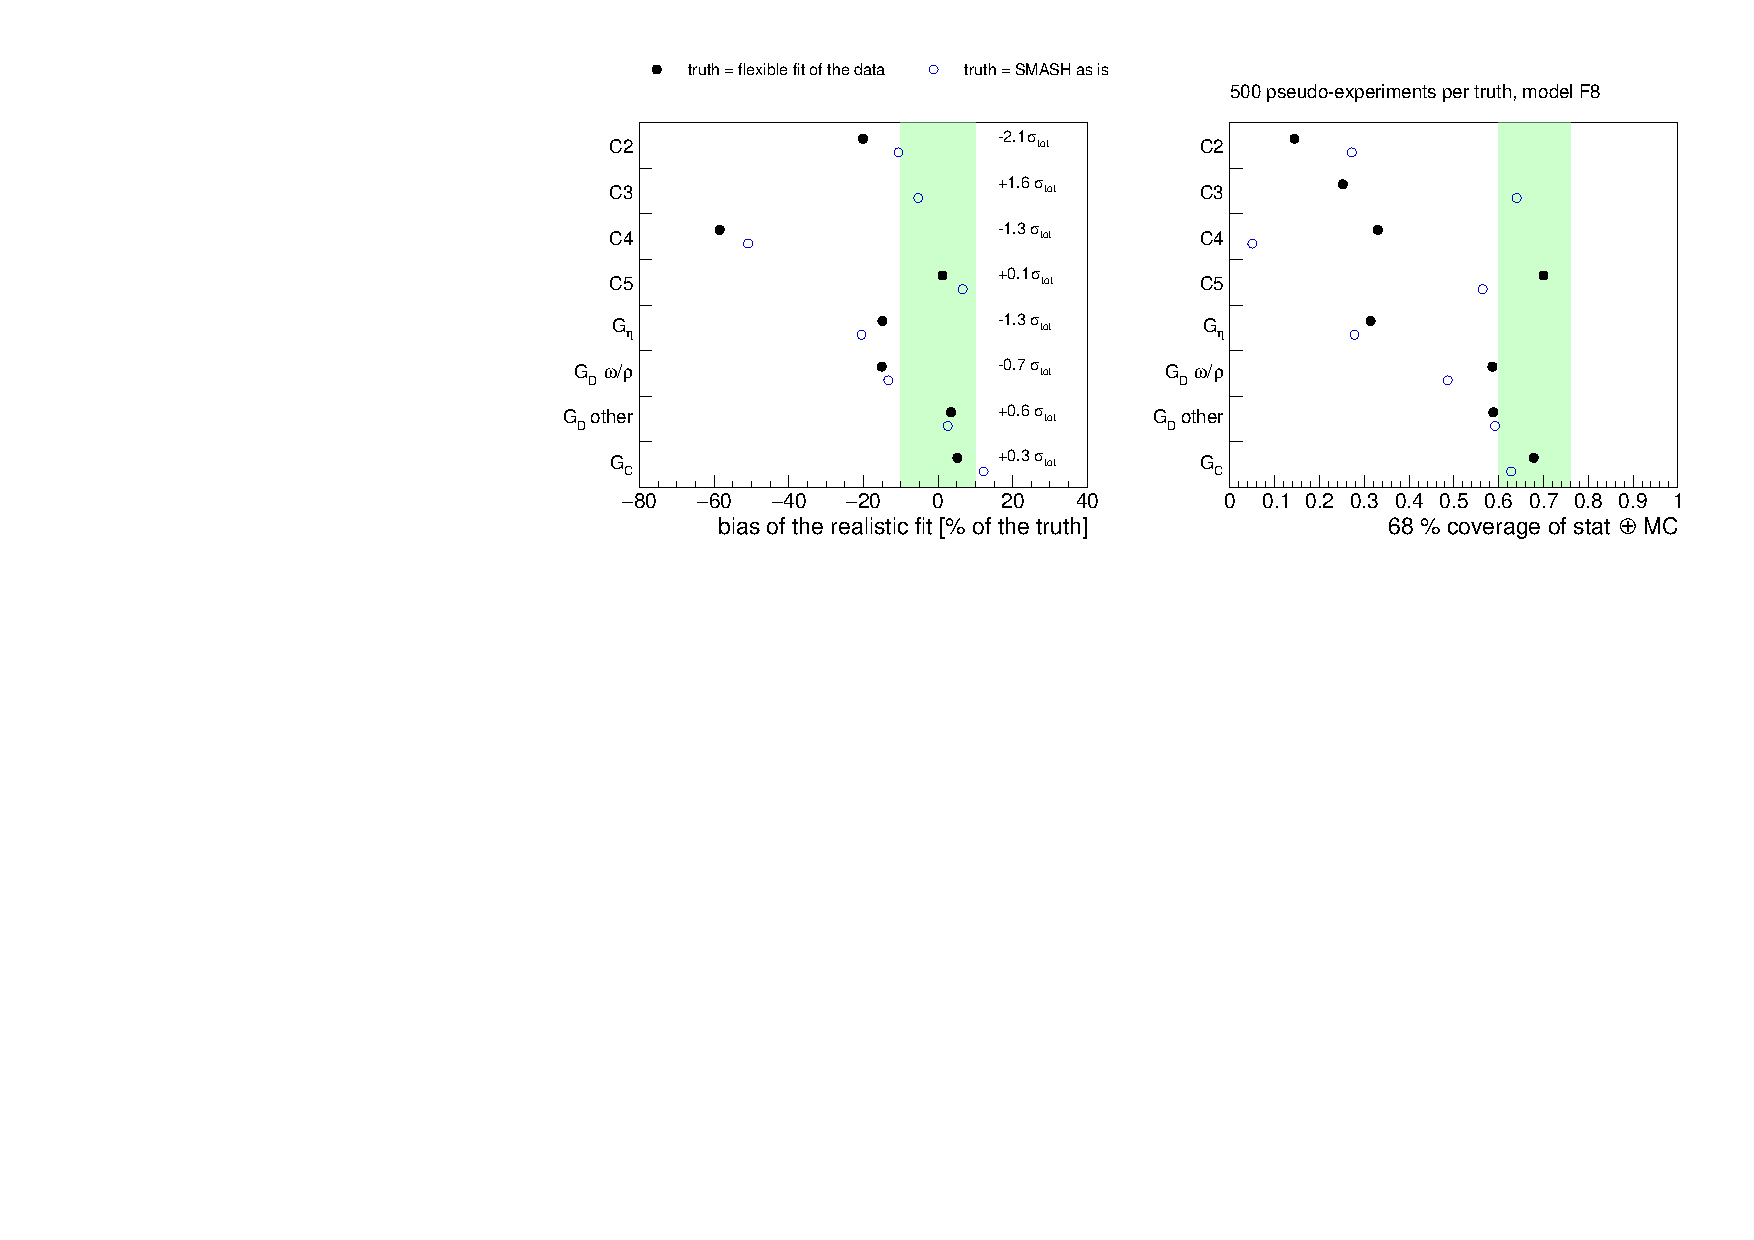
\includegraphics[width=0.84\textwidth]{figs_all/flex_bias_v2.pdf}
\caption{\textbf{What it shows: with the real template noise the fit attenuates C2, C4, \Geta and $G_D(\omega/\rho)$; only C5, $G_C$ and (marginally)
$G_D$(other) are recovered within the limits.}
Selection: pseudo-data in the bins of the nominal flexible fit (the nominal cuts S0 (PT3 trigger; event vertex in the target region, $\vz>-160$\,mm; START-free \betanew identification, pions within 3$\sigma$, leptons within 5$\sigma$ with a RICH ring; energy-loss-corrected momenta of all four tracks; both pions used in the event-vertex fit; all stored combinations of an event, isBest $\ge0$); \Mee$\ge10$\,\MeVcc; five \Mpipi slices (below 0.34, 0.34--0.37, 0.37--0.39, 0.39--0.43, from 0.43\,\GeVcc); \Mfour 0.40--0.70\,\GeVcc, 70 bins per slice (5\,\MeVcc; 2.5\,\MeVcc in 0.52--0.57), 350 bins): truth from the full SMASH simulation (mode A, $w\times$V3, simulated \Mfour$\times0.99615$ and \Mpipi$\times0.9952$) with known scales, plus the CB of the data ($2\sqrt{N_{++}N_{--}}$ of the like-sign data, with the noise of the 200 CB replicas), Poisson counts; fitted with the templates of another simulation bootstrap replica.
Bias test of F8, 500 pseudo-experiments per truth, templates from bootstrap replicas. Left: bias of the realistic fit in per cent of the truth
(right column: in units of $\sigma_{\mathrm{tot}}$, truth $=$ the fit); right: 68\,\% coverage of stat $\oplus$ MC. Black full: truth $=$ the flexible
fit of the data; blue open: truth $=$ SMASH as is. Green bands: the pass limits ($\pm10$\,\%; 0.60--0.76). C3 (truth $-0.09$) is judged in $\sigma$
units only.}
\label{fig:flex-bias}
\end{figure}

\subsection{Variants and the comparison with Part III}
\label{sec:flex-var}

\begin{table}[H]
\centering
\caption{\textbf{What it shows: the signal scales stay within about 0.25--0.55 (C2) and 0.44--0.69 (C5) over the usable variants, while the background
scales move by factors; the 0.40--1.00 fits need unphysical values.} Model F8 unless stated; value (total error where printed); hybrid GLS
$\chi^2$/ndf. Source: \code{tables_all/flex_variants.txt}.}
\label{tab:flex-var}
\footnotesize
\setlength{\tabcolsep}{2.5pt}
\resizebox{\textwidth}{!}{%
\begin{tabular}{@{}l r r r r r r r r r l@{}}
\toprule
variant & $\chi^2$/ndf & C2 & C3 & C4 & C5 & \Geta & $G_D(\omega/\rho)$ & $G_D$(other) & $G_C$ & extra \\
\midrule
nominal F8 & 604/342 & 0.41 & $-0.09$ & 0.34 & 0.63 & 2.10 & 0.79 & 1.11 & 1.60 & \kEtwo 0.91 \\
alternative F7bj & 603/338 & 0.48 & $-0.06$ & 0.37 & 0.66 & 1.39 & \multicolumn{2}{c}{1.07 (one $G_D$)} & 1.80 & \kEtwo 0.93, tilts \\
E2 split 10--20 / $\ge20$\,\MeVcc & 1114/692 & $0.31\pm0.04$ & $0.26\pm0.10$ & $0.38\pm0.12$ & $0.55\pm0.09$ & $1.85\pm0.21$ & $0.60\pm0.13$ & $1.21\pm0.06$ & $1.66\pm0.07$ & \kEtwo $0.76\pm0.08$ \\
$+$E1, \kEone free & 1454/691 & $0.26\pm0.04$ & $0.32\pm0.05$ & $0.34\pm0.06$ & $0.52\pm0.11$ & $1.93\pm0.21$ & $0.63\pm0.15$ & $1.25\pm0.06$ & $1.38\pm0.04$ & \kEone $4.4\pm1.6$ \\
$+$E1, $s_{T3}$ free & 1500/691 & 0.25 & 0.33 & 0.36 & 0.51 & 2.13 & 0.73 & 1.30 & $1.07\pm0.20$ & $s_{T3}$ $0.71\pm0.37$ \\
$+$E1, E2a, E2b & 2228/1041 & 0.25 & 0.31 & 0.36 & 0.46 & 1.57 & 0.45 & 1.42 & 1.39 & \kEtwo $0.40\pm0.10$ \\
\Mfour 0.42--0.70 & 547/322 & 0.42 & $-0.06$ & 0.30 & 0.58 & 1.37 & 0.43 & 1.03 & 2.44 & \\
\Mfour 0.45--0.70 & 456/292 & 0.37 & 0.25 & 0.28 & 0.55 & 1.13 & 0.30 & 1.02 & 2.69 & \\
raw $G_D$, $G_C$ templates & 412/342 & 0.31 & 0.06 & $-0.30\pm0.46$ & $0.94\pm0.17$ & 1.95 & 0.71 & 1.40 & 0.70 & \\
fake-lepton T3 added in E2 & 613/341 & 0.42 & 0.32 & 0.43 & 0.44 & $0.31\pm0.25$ & 0.34 & 0.88 & $0.04\pm0.64$ & $s_{T3}$ $5.6\pm1.0$ \\
\midrule
\Mfour 0.40--1.00, smoothed per piece & 1308/492 & 0.29 & $-0.09$ & 0.52 & 0.37 & 5.91 & 1.70 & 1.57 & $\mathbf{-2.28}$ & \kEtwo 1.42 \\
\Mfour 0.40--1.00, raw background & 1835/492 & 0.38 & 0.15 & 0.56 & 1.22 & 4.50 & 1.33 & 1.01 & 0.00 & \kEtwo $1.38\pm0.05$ \\
\bottomrule
\end{tabular}}
\end{table}

\textbf{The class \Mee$<10$\,\MeVcc.} With it the conversion classes become determined (C3 0.32, C4 0.34 $\pm$ 0.05--0.06, $G_C$ 1.38 $\pm$ 0.04), but
that class needs an extra CB-like term ($\kEone=4.4\pm1.6$) or a fake-lepton term ($s_{T3}=0.71\pm0.37$), which describe it about equally
(hybrid 1454 against 1500 for 691 degrees of freedom); its CB is not understood (as Part~III's $\kEone=7.6$). Fixing $\kEone=1$ moves C3 and C4 by at
most 0.06 and $G_C$ by up to 0.38: these values are \emph{conditional on the E1 model}, mainly for $G_C$. With E2 split at 20\,\MeVcc the CB scale
falls to $0.76\pm0.08$ (0.40 with E1 too): the CB spread over the \Mee cells is not consistent with $k=1$ per cell, as WP0 warned. Once the
fake-lepton template is allowed in E2 it takes 5.6 $\times$ SMASH and pushes \Geta to 0.3 and $G_C$ to 0: \Geta, $G_C$ and $G_D$ cannot be
separated with \Mee$\ge10$\,\MeVcc, and any statement on \Geta alone is model-dependent.

\textbf{Comparison with Part~III} (its F-main, reproduced; the Part~III-equivalent of each scale; Fig.~\ref{fig:flex-cmp}): $\aEta=0.382\pm0.043$
against $s_{\mathrm{C2}}=0.41\pm0.07$ (F7bj $0.48\pm0.08$); $a\rhod=0.50\pm0.10$ against $s_{\mathrm{C5}}=0.63\pm0.12$ ($0.66\pm0.12$); $\rhod=1.32\pm0.25$
against $s_{\mathrm{C5}}/s_{\mathrm{C2}}=1.52\pm0.52$ ($1.37\pm0.41$); $\kappa=0.83\pm0.30$ against $s_{\mathrm{C4}}/s_{\mathrm{C2}}=0.81\pm0.66$; the
$G_D$-weighted $c_j(1+bx)=1.06\pm0.16$ against $s_{GD}$(other) $=1.11\pm0.11$; $c_j\kB=2.07\pm0.67$ against $s_{GC}=1.60\pm0.69$; $\kEtwo$ $0.98\pm0.07$
against $0.91\pm0.06$; $ag=0.66\pm0.12$ against $s_{G\eta}=2.10\pm0.59$. They agree within 1$\sigma$ except \Geta, whose difference is not robust
(\S\ref{sec:flex-robust}; Part~III's $\kappa$ and $g$ were largely set by their priors).

\begin{figure}[!htbp]
\centering
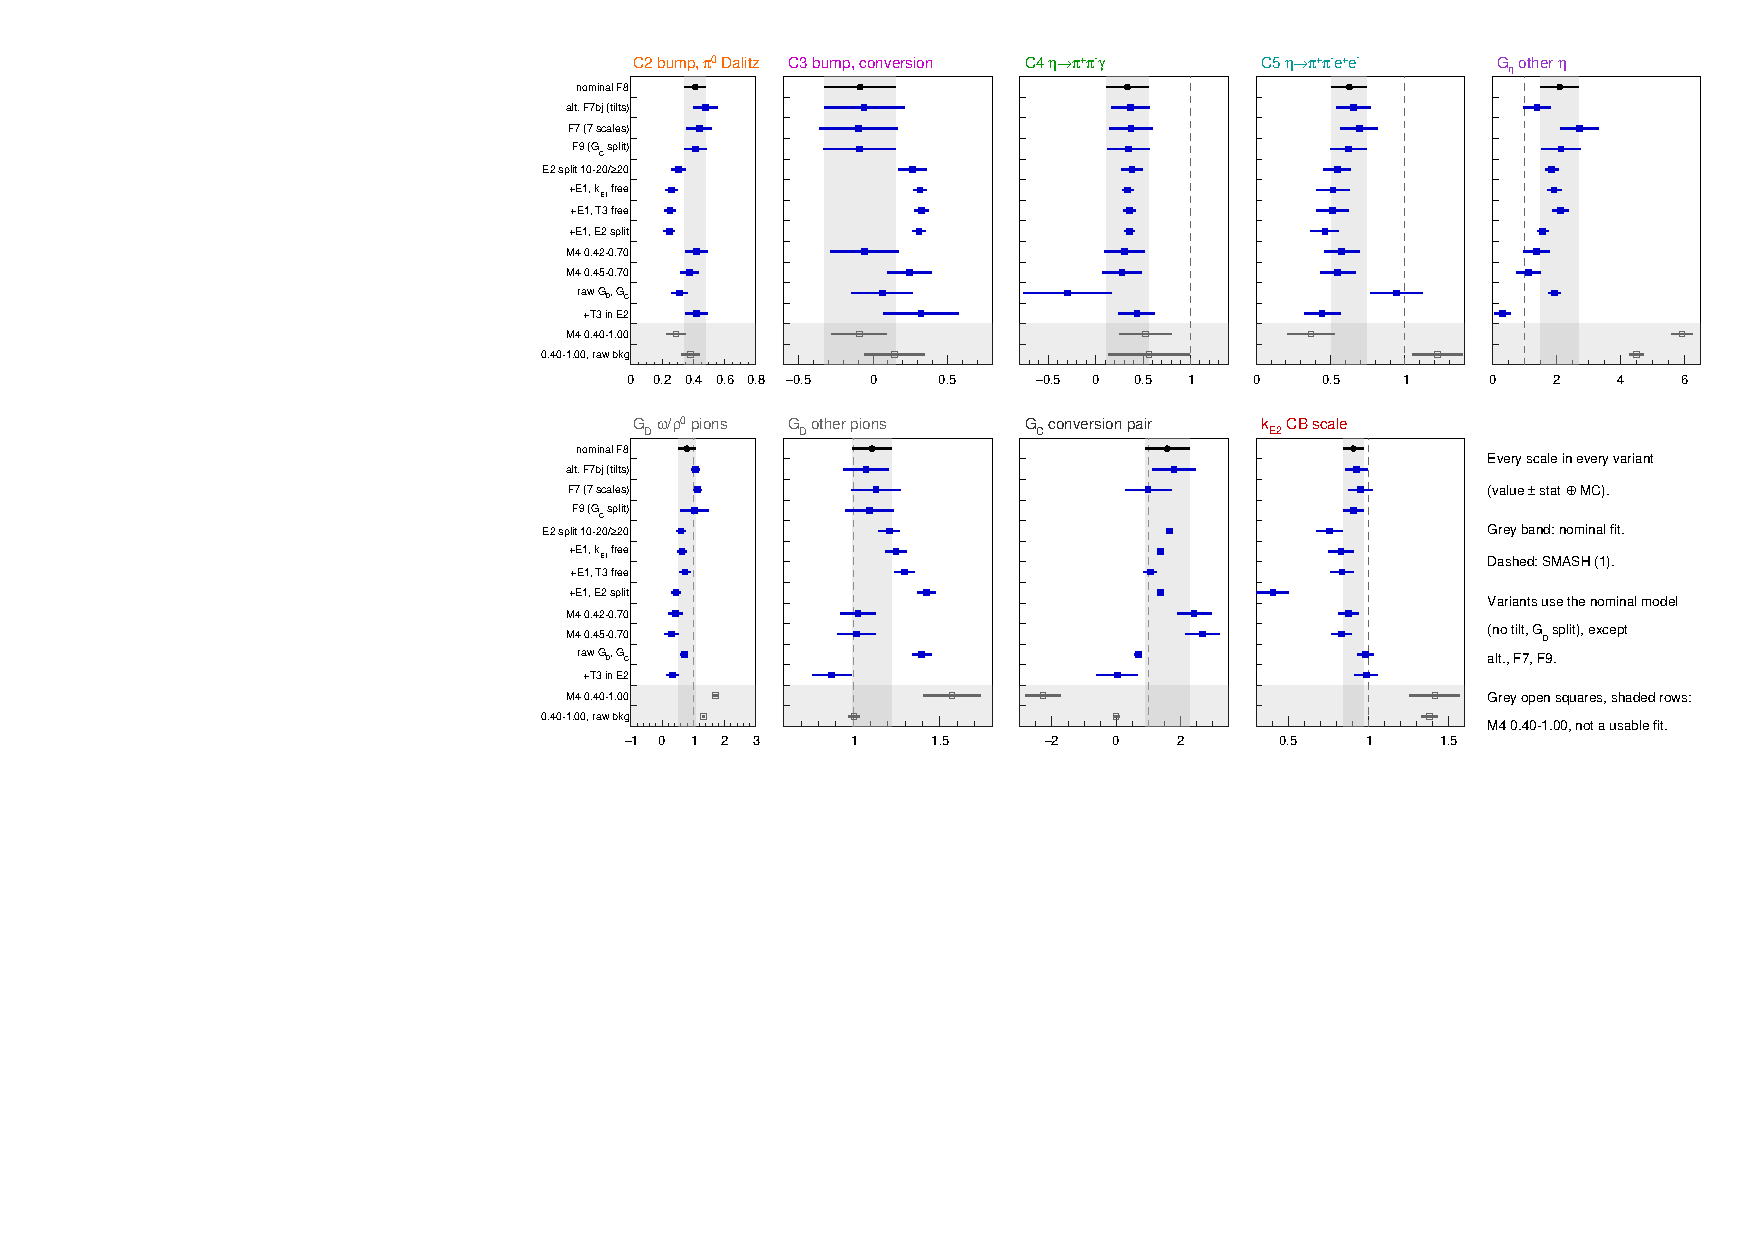
\includegraphics[width=\textwidth]{figs_all/flex_variants_v2.pdf}
\caption{\textbf{What it shows: over the usable variants the $\eta$ signal scales stay together (C2 0.25--0.54, C5 0.44--0.69), while \Geta, $G_C$ and
$G_D(\omega/\rho)$ move by large factors; the 0.40--1.00 fits are not usable.}
Selection: data at $L=6079.2\,\nbinv$ with the nominal cuts S0 (PT3 trigger; event vertex in the target region, $\vz>-160$\,mm; START-free \betanew identification, pions within 3$\sigma$, leptons within 5$\sigma$ with a RICH ring; energy-loss-corrected momenta of all four tracks; both pions used in the event-vertex fit; all stored combinations of an event, isBest $\ge0$); CB $=2\sqrt{N_{++}N_{--}}$ of the like-sign data with the same cuts (10\,\MeVcc cells of \Mfour, shared over the \Mpipi and \Mee cells by the like-sign share of each 50\,\MeVcc band), times a factor $k$ fitted within $1\pm0.05$ (for \Mee$\ge10$\,\MeVcc); SMASH (standard, lepton and $\eta$ sets, 221.05\,\nbinv each, every count from one set only, mode A; every channel at its SMASH cross section $\times$ PDG BR $\times$ the $\eta$-decay weights V3; simulated \Mfour$\times0.99615$, \Mpipi$\times0.9952$), with the same cuts. Nominal bins: \Mee$\ge10$\,\MeVcc; five \Mpipi slices (below 0.34, 0.34--0.37, 0.37--0.39, 0.39--0.43, from 0.43\,\GeVcc); \Mfour 0.40--0.70\,\GeVcc, 70 bins per slice (5\,\MeVcc; 2.5\,\MeVcc in 0.52--0.57), 350 bins. The variants change the bins as their names say: \Mee 10--20 and $\ge20$\,\MeVcc fitted as separate classes; the class \Mee$<10$\,\MeVcc added (``$+$E1''); \Mfour 0.42--0.70, 0.45--0.70 or 0.40--1.00\,\GeVcc (10\,\MeVcc bins above 0.70); the other variants (raw background templates, the fake-lepton term, F7, F9, F7bj) keep the nominal bins.
Every scale (panel titles in the channel colours) in every variant: value $\pm$ stat $\oplus$ MC. Black: nominal F8; blue squares: variants; grey
band: the nominal fit; dashed: SMASH (1). The variants use the nominal model (no tilt, $G_D$ split) except ``alt.\ F7bj'', F7 and F9. Grey open
squares in the shaded rows: \Mfour 0.40--1.00, not a usable fit (\S\ref{sec:flex-r100}).}
\label{fig:flex-var}
\end{figure}

\begin{figure}[!htbp]
\centering
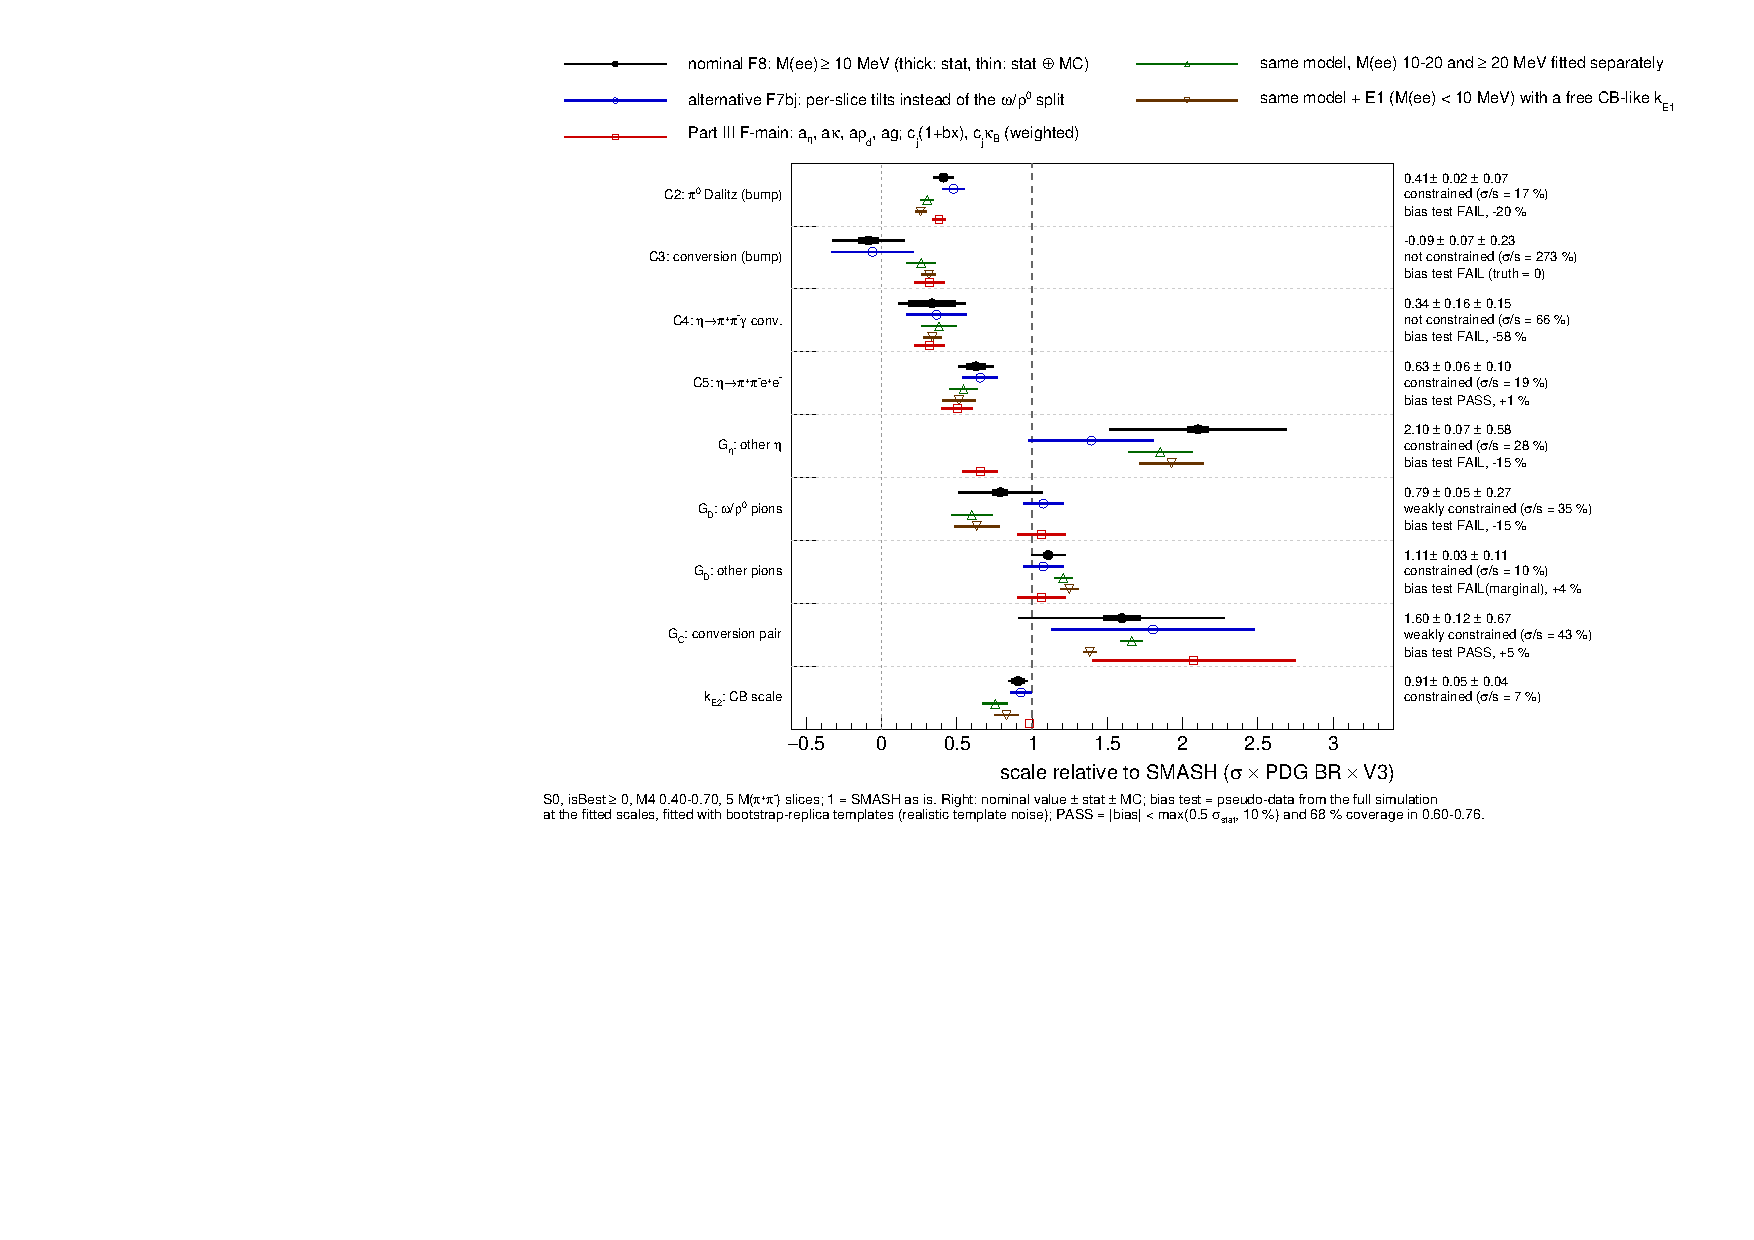
\includegraphics[width=0.94\textwidth]{figs_all/flex_scales_cmp_v2.pdf}
\caption{\textbf{What it shows: the flexible scales agree with the Part~III values within about 1$\sigma$ except \Geta, which is not robust; the
signal scales hardly depend on the variant.}
Selection: data at $L=6079.2\,\nbinv$ with the nominal cuts S0 (PT3 trigger; event vertex in the target region, $\vz>-160$\,mm; START-free \betanew identification, pions within 3$\sigma$, leptons within 5$\sigma$ with a RICH ring; energy-loss-corrected momenta of all four tracks; both pions used in the event-vertex fit; all stored combinations of an event, isBest $\ge0$); CB $=2\sqrt{N_{++}N_{--}}$ of the like-sign data with the same cuts (10\,\MeVcc cells of \Mfour, shared over the \Mpipi and \Mee cells by the like-sign share of each 50\,\MeVcc band), times a factor $k$ fitted within $1\pm0.05$ (for \Mee$\ge10$\,\MeVcc); SMASH (standard, lepton and $\eta$ sets, 221.05\,\nbinv each, every count from one set only, mode A; every channel at its SMASH cross section $\times$ PDG BR $\times$ the $\eta$-decay weights V3; simulated \Mfour$\times0.99615$, \Mpipi$\times0.9952$), with the same cuts. Black, blue and the red Part~III values (F-main): \Mee$\ge10$\,\MeVcc; five \Mpipi slices (below 0.34, 0.34--0.37, 0.37--0.39, 0.39--0.43, from 0.43\,\GeVcc); \Mfour 0.40--0.70\,\GeVcc, 70 bins per slice (5\,\MeVcc; 2.5\,\MeVcc in 0.52--0.57), 350 bins; green: the same with \Mee 10--20 and $\ge20$\,\MeVcc fitted as separate classes; brown: the class \Mee$<10$\,\MeVcc added.
Every scale against 1 (SMASH as is, dotted). Black: nominal F8 (thick bar stat, thin bar stat $\oplus$ MC); blue open circles: alternative F7bj;
green triangles: \Mee 10--20 and $\ge20$\,\MeVcc fitted separately; brown triangles: with the class \Mee$<10$\,\MeVcc and a free CB-like \kEone; red
open squares: the Part~III-equivalent of each scale ($a_\eta$, $a\kappa$, $a\rho_d$, $ag$, $c_j(1+bx)$, $c_j\kB$, weighted; both $G_D$ rows show
the same Part~III value). Right column: the nominal value $\pm$ stat $\pm$ MC, the constraint class of the package (total relative error below 30\,\%, judged before the fit-method test, so ``constrained'' does not make \Geta a determination, \S\ref{sec:flex-robust}) and the bias-test verdict. S0, isBest $\ge0$,
\Mfour 0.40--0.70\,\GeVcc.}
\label{fig:flex-cmp}
\end{figure}

\subsection{Above \texorpdfstring{\Mfour$=0.70$\,\GeVcc}{M4 = 0.70 GeV/c2}}
\label{sec:flex-r100}
Extended to 1.00\,\GeVcc (Figs.~\ref{fig:flex-r100}, \ref{fig:flex-r100asis}), the fits need unphysical or extreme scales: $G_C=-2.3$ (smoothed per piece) or 0 (raw
background), \Geta 4.5--5.9, \kEtwo 1.38--1.42, 7--8$\sigma$ from its constraint; Pearson $\chi^2$/ndf 3.7--7.5. The smoothing itself fails there
for the $G_D(\omega/\rho)$ template of S5 ($\chi^2=228$ for 30 bins: exp(pol3) cannot follow the $\rho^0$/$\omega$ structure). An independent check
of SMASH as is (verifier, \Mee$\ge10$\,\MeVcc, all slices) shows why: $(N-\mathrm{CB})$/SMASH falls from 1.20--1.23 in 0.575--0.675 to 1.14, 1.10 and
1.08 up to 0.75\,\GeVcc and stays at 1.08--1.15 up to 0.85\,\GeVcc, while the composition of SMASH stays nearly fixed ($G_D$ 73--77\,\%, $G_C$
18--20\,\%, \Geta 5--6\,\%). Per-channel scales cannot follow a drift of about 10\,\% at fixed composition. \textbf{The scales of 0.40--0.70 must not
be carried above 0.70.} One candidate for the difference is the target material (13--15\,\% of $N-\mathrm{CB}$ in 0.40--0.70, not simulated); it is
not resolved here.

\begin{figure}[p]
\centering
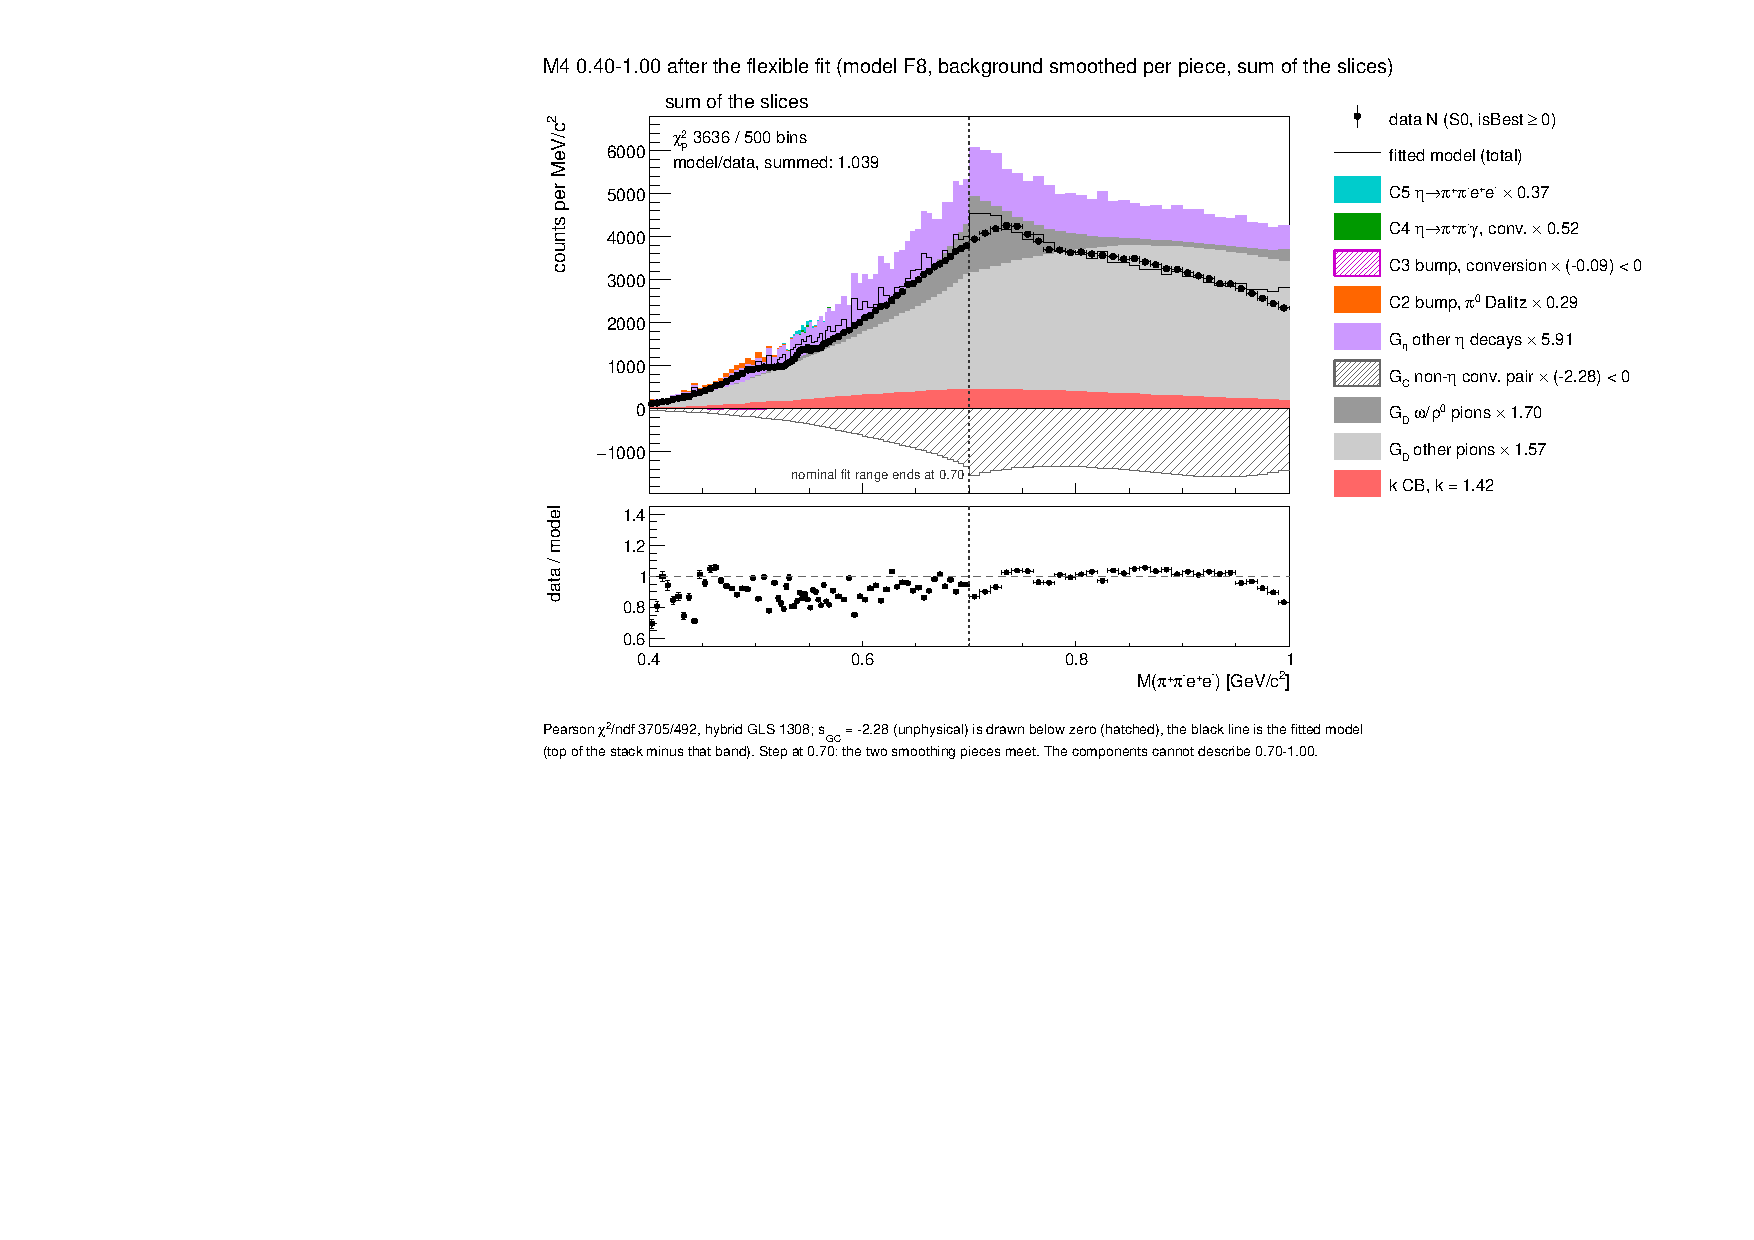
\includegraphics[width=0.78\textwidth]{figs_all/flex_r100_v2_cnt.pdf}\\[-0.2em]{\small (a)}\\[0.4em]
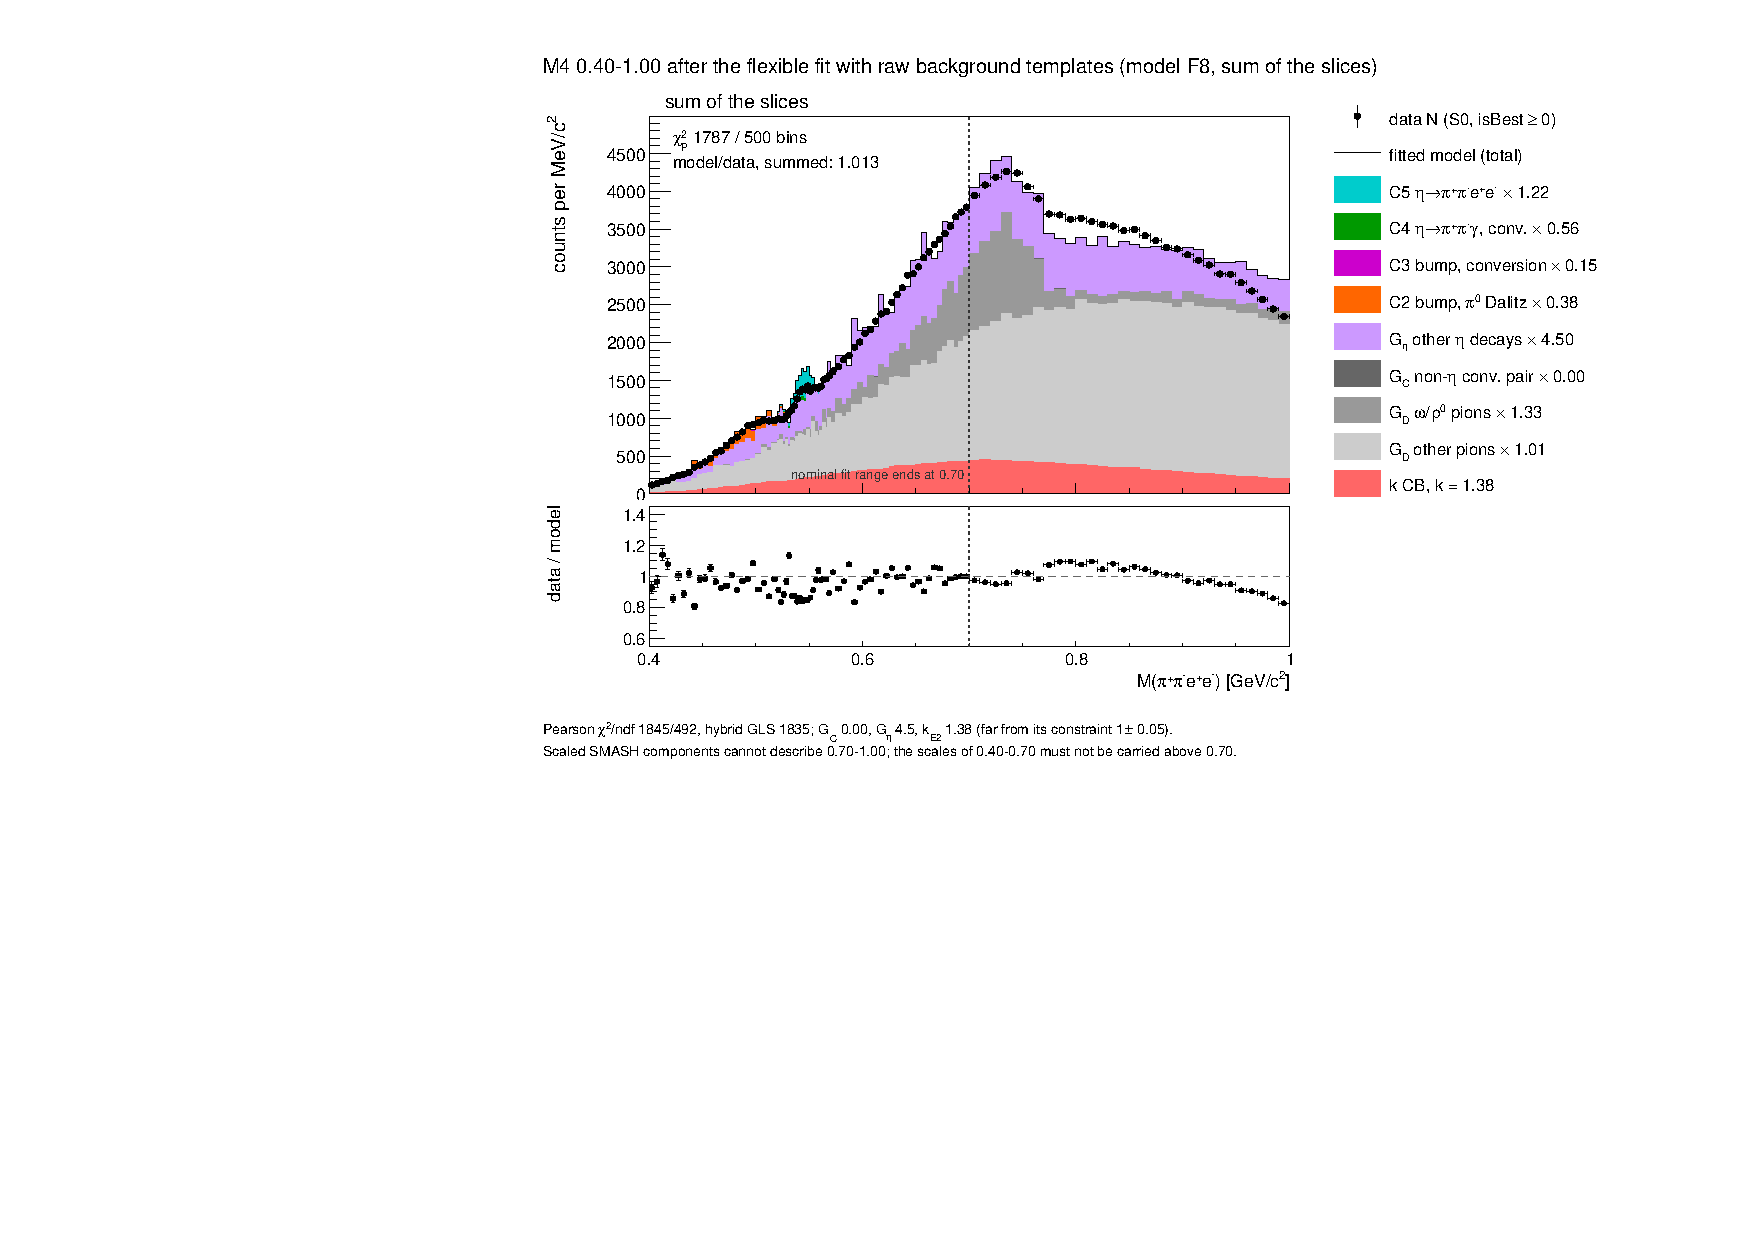
\includegraphics[width=0.78\textwidth]{figs_all/flex_r100raw_v2_cnt.pdf}\\[-0.2em]{\small (b)}
\caption{\textbf{What it shows: with scaled SMASH components the region 0.70--1.00\,\GeVcc cannot be described; the fits need a negative or
vanishing $G_C$, a large \Geta and a CB scale far from its constraint.}
Selection: data and SMASH with the nominal cuts S0 (PT3 trigger; event vertex in the target region, $\vz>-160$\,mm; START-free \betanew identification, pions within 3$\sigma$, leptons within 5$\sigma$ with a RICH ring; energy-loss-corrected momenta of all four tracks; both pions used in the event-vertex fit; all stored combinations of an event, isBest $\ge0$); \Mee$\ge10$\,\MeVcc; five \Mpipi slices (below 0.34, 0.34--0.37, 0.37--0.39, 0.39--0.43, from 0.43\,\GeVcc) fitted, summed here; \Mfour 0.40--1.00\,\GeVcc (nominal bins to 0.70, then 10\,\MeVcc); CB $=2\sqrt{N_{++}N_{--}}$ of the like-sign data ($k$ fitted within $1\pm0.05$); SMASH mode A, $w\times$V3, \Mfour$\times0.99615$, \Mpipi$\times0.9952$.
\Mfour 0.40--1.00\,\GeVcc, sum of the slices, \Mee$\ge10$\,\MeVcc, data $N$ (black points), raw counts per \MeVcc; dotted line: end of the nominal fit
range at 0.70. Stack: $k\,$CB (red), $G_D$ other pions (light grey) and $\omega/\rho^0$ pions (mid grey), $G_C$ (dark grey), \Geta (violet), C2
(orange), C3 (magenta), C4 (green), C5 (cyan). Negative terms are hatched below zero; the black line is the fitted model (top of the stack minus the
hatched part). (a) F8 with the background smoothed per piece (0.40--0.70, 0.70--1.00): $s_{GC}=-2.28$ (unphysical, hatched), \Geta 5.91,
$k=1.42$; Pearson 3705/492, hybrid GLS 1308; the step at 0.70 is where the two smoothing pieces meet. (b) F8 with raw background templates: $G_C$
0.00, \Geta 4.50, $k=1.38$ (constraint $1\pm0.05$); Pearson 1845/492, hybrid 1835. Panel $\chi^2_P=\sum(N-\mu)^2/V$ leaves out the \kEtwo
constraint term. SMASH as is over the same range: Fig.~\ref{fig:flex-r100asis}.}
\label{fig:flex-r100}
\end{figure}

\begin{figure}[!htb]
\centering
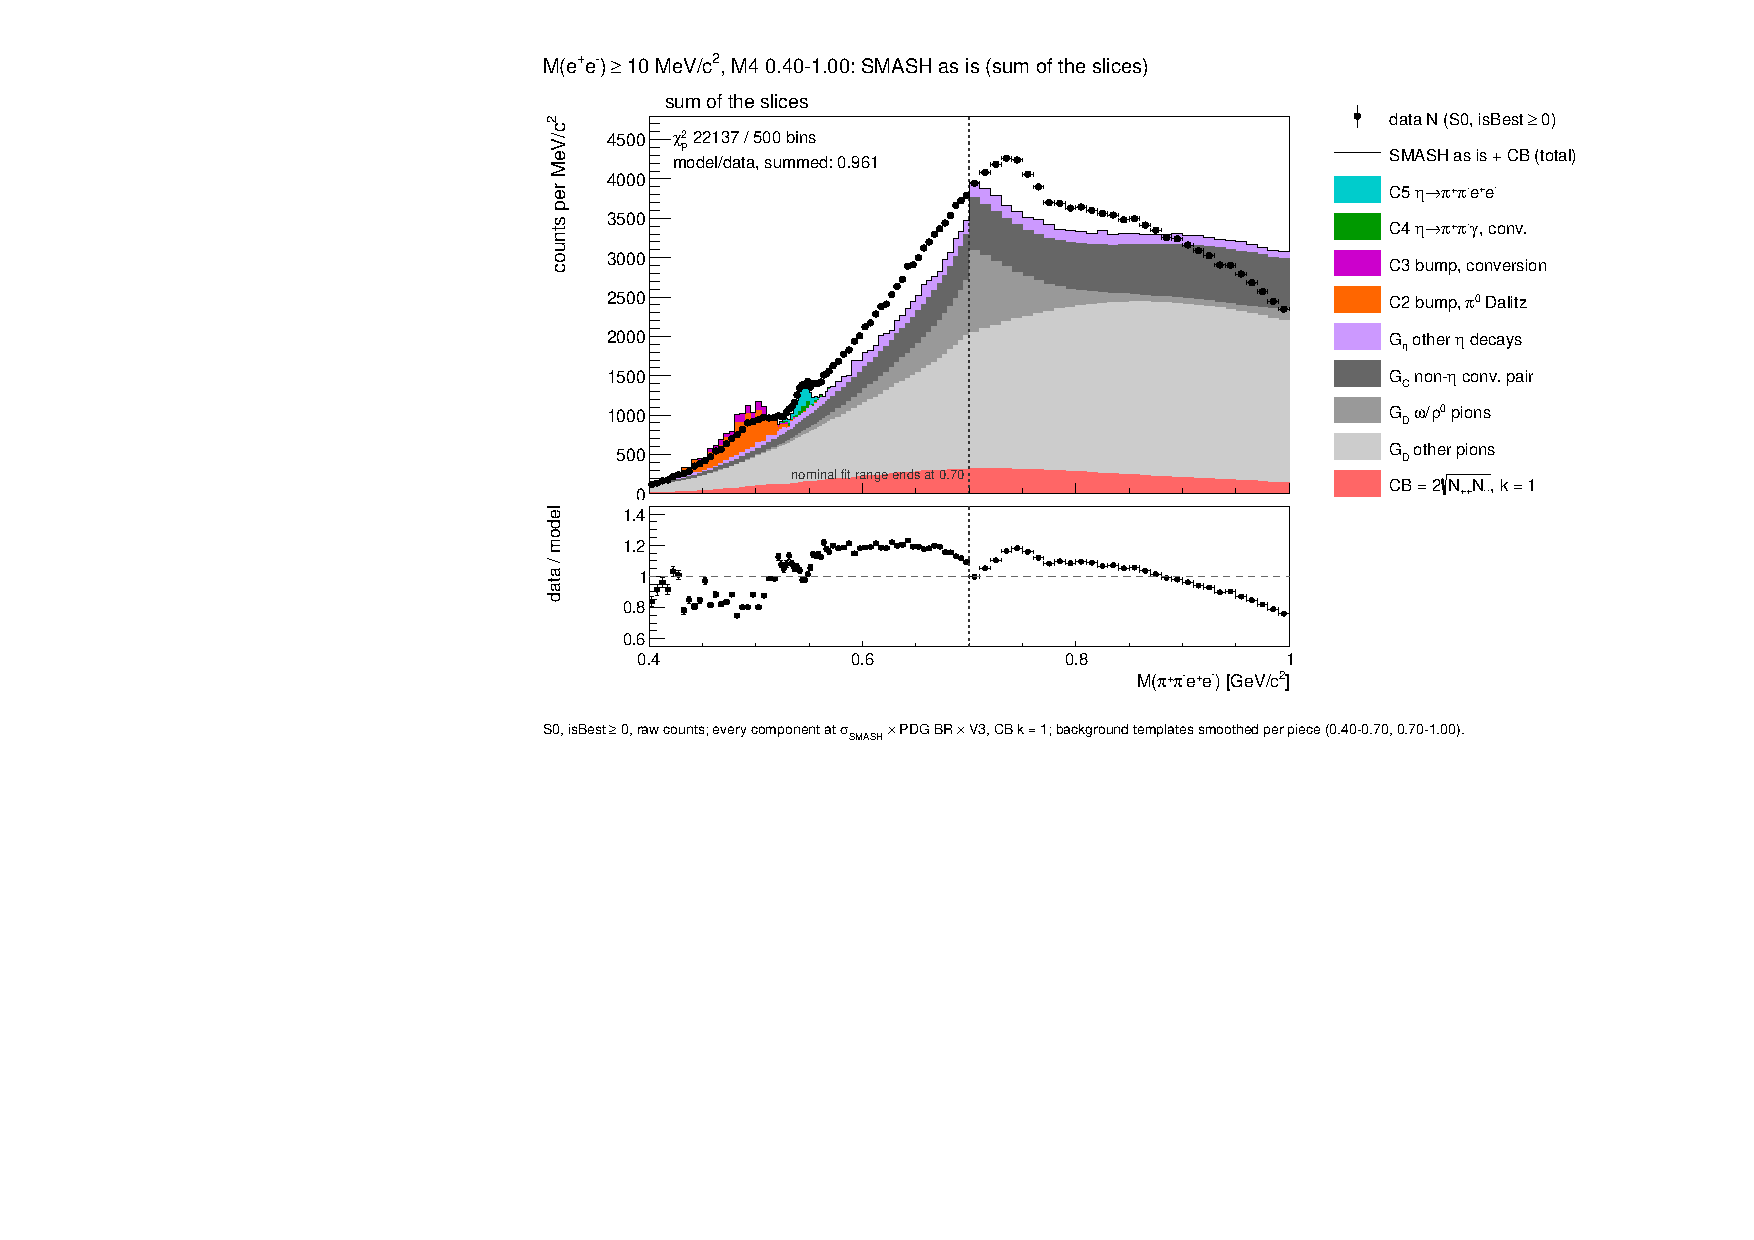
\includegraphics[width=0.80\textwidth]{figs_all/flex_r100_asis_v2_cnt.pdf}
\caption{\textbf{What it shows: SMASH as is over \Mfour 0.40--1.00\,\GeVcc: too high in the bump, about 20\,\% too low just above the peak, and
above the data at the high-mass end (data/model 0.76 at 1.0\,\GeVcc).}
Selection: as Fig.~\ref{fig:flex-r100}: data at $L=6079.2\,\nbinv$ with the nominal cuts S0 (PT3 trigger; event vertex in the target region, $\vz>-160$\,mm; START-free \betanew identification, pions within 3$\sigma$, leptons within 5$\sigma$ with a RICH ring; energy-loss-corrected momenta of all four tracks; both pions used in the event-vertex fit; all stored combinations of an event, isBest $\ge0$); \Mee$\ge10$\,\MeVcc; the five \Mpipi slices summed; \Mfour 0.40--1.00\,\GeVcc (nominal bins up to 0.70, then 10\,\MeVcc bins); CB $=2\sqrt{N_{++}N_{--}}$ of the like-sign data with the same cuts (10\,\MeVcc cells of \Mfour, $k=1$, shared over the \Mpipi and \Mee cells by the like-sign share of each 50\,\MeVcc band); SMASH (standard, lepton and $\eta$ sets, 221.05\,\nbinv each, every count from one set only, mode A; every channel at its SMASH cross section $\times$ PDG BR $\times$ the $\eta$-decay weights V3; simulated \Mfour$\times0.99615$, \Mpipi$\times0.9952$), with the same cuts; no parameter fitted.
As Fig.~\ref{fig:flex-r100}, every component at its SMASH cross section $\times$ PDG BR $\times$ V3 and CB with $k=1$ (black line: the total);
background templates smoothed per piece. Panel $\chi^2_P$ 22\,137 for 500 bins; summed model/data 0.961.}
\label{fig:flex-r100asis}
\end{figure}

\subsection{Conclusions in plain words}
\label{sec:flex-concl}
\begin{enumerate}\setlength{\itemsep}{1pt}
\item \textbf{The $\eta$ signal classes are below SMASH by one common factor.} C2, C4 and C5 are consistent with one $\eta$ scale,
      $0.46\pm0.06$ ($p=0.21$), $0.57\pm0.07$ after the template-noise correction ($p=0.51$), in line with the peak (0.42) and the bump edge
      (0.39--0.43).
\item \textbf{The direct decays} give $0.63\pm0.12$ with about $\pm0.1$ from the model and the fit method (0.44--0.94 over the variants); C5/C2 agrees
      with the PDG ratio within 1--2$\sigma$.
\item \textbf{The non-$\eta$ background in 0.565--0.70\,\GeVcc is 10--30\,\% above SMASH}; how it splits between $G_D$, $G_C$ and \Geta is not
      determined (80--90\,\% correlated, and the split moves with the fit method).
\item \textbf{The conversion classes} need \Mee$<10$\,\MeVcc, whose CB is not understood; their values (0.32--0.34) are conditional on the model of
      that class.
\item \textbf{The template noise of the simulation dominates} (MC error 1--8 times the statistical one; C2 $-20$\,\%, C4 $-58$\,\% in the pseudo-data
      test). A larger SMASH production is the most useful single improvement.
\item \textbf{The scales cannot be carried above \Mfour$=0.70$\,\GeVcc}, and \textbf{the flexible model is still incomplete} ($p<0.001$; the fitted
      model is 2\,\% above the data, 5.8\,\% in the peak window).
\item \textbf{The model choice is a documented convention} (D36): the ladder statistic cannot rank nested models, and the scales are a description,
      not measurements.
\end{enumerate}

\textbf{Verification} (vflex: own dump of the factory histograms, own fitter and solver, 2000 own pseudo-data sets). Numbers confirmed: every
scale and error to $10^{-6}$, the information shares, the bias test and its verdicts. Conclusions only partly confirmed; the changes requested
are made above: $p<0.001$ instead of 0.002; a fit-method systematic stated, and \Geta, $G_C$, $G_D(\omega/\rho)$ and ``the true C2 $\approx0.52$''
removed as determinations; the ladder not used as a significance; the $\eta$ statement limited to C2, C4, C5 and C5/C2 ``within 1--2$\sigma$'';
the $+2$\,\% overshoot named; and the figures redrawn in the Part~III palette with negative terms hatched below zero (\code{flex_figs_v2.C}).

%======================================================================
\section{Search for X17 in \texorpdfstring{$\eta\to\pi^+\pi^-X17$}{eta -> pi+pi-X17}, \texorpdfstring{$X17\to e^+e^-$}{X17 -> e+e-}}
\label{sec:x17}
%======================================================================
\inshort{no X17 signal. The 90\,\% CL$_s$ upper limit is $r<0.114$, i.e.\ $\BRX<3.16\times10^{-5}$ at 17\,\MeVcc with the PDG 2026 BR$(\eta\to\ppee)$ ($3.06\times10^{-5}$ with the PDG 2020 value of the frozen procedure; expected $2.7\times10^{-5}$), from a two-dimensional fit frozen before the unblinding (blind in the code, not in the information: Part~II had shown the \Mee shape of the peak band); a one-window count would give only $<2.6\times10^{-4}$. The BESIII limit near 17\,\MeVcc is about two times stronger; the HADES preliminary value is numerically similar but built differently, so it is not a cross-check (\S\ref{sec:x17other}).}
\notebox{\textbf{In plain words: no X17 signal is seen.} The 90\,\% CL$_s$ upper limit is $\BRX<3.16\times10^{-5}$ at 17\,\MeVcc (PDG 2026), against an
expected $2.7\times10^{-5}$ ($\pm1\sigma$: 1.5--4.9$\times10^{-5}$); X17 contributes at most 11\,\% of the direct decays $\eta\to\ppee$; across
10--40\,\MeVcc the limit runs from $4.0\times10^{-5}$ to $0.9\times10^{-5}$; the procedure was frozen before the unblinding. A simple count with
\code{TRolke} gives $2.6\times10^{-4}$ (\S\ref{sec:trolke}).\\[0.4em]
\textbf{Result in detail.} 90\,\% CL$_s$ upper limit on \BRX at $m_X=16.7$, 16.85 and 17.0\,\MeVcc: $\mathbf{3.16\times10^{-5}}$ (normalisation
(1), primary; S0, isBest $\ge0$, $L=6079.2\,\nbinv$), i.e.\ $r_{\mathrm{UL}}=0.114$ times BR$(\eta\to\ppee)=2.76\times10^{-4}$ (PDG 2026, ruling D25);
$3.06\times10^{-5}$ with the PDG 2020 value $2.68\times10^{-4}$ frozen before the unblinding. The frozen likelihood was rerun with only BR$_{\mathrm{dir}}$
changed to PDG 2026 (its uncertainty in $s_X$ 4.1 $\to$ 5.8\,\%): $r_{\mathrm{UL}}$ moves by $+0.13$\,\% (0.11431 $\to$ 0.11445 at 17\,\MeVcc), $Z$ and
$\hat r$ do not change; the toy-based numbers are the frozen ones $\times1.0299\,k$ ($k=1.0011$--1.0014, the rerun ratio at that mass). \textbf{Hypothesis}: a prompt spin-0 X17 (isotropic $e^+$ angle, three-body phase
space in \Mpipi); for a vector-like X17 ($1+\cos^2\theta$, as a photon in $\eta\to\pipi\gamma$) the limit is $\mathbf{3.79\times10^{-5}}$.
\textbf{Normalisation}: (1) failed the slope test on the 1500 toys of the specification (0.673, coverage 0), whose fall-back makes (2) primary
($3.29\times10^{-5}$; 3.28 with the PDG 2020 BR$(\eta\to\pipi\piz)$ in its $\eta$ scale \aEta); (1) was kept on smooth-parent toys built afterwards (slope 1.024, coverage 0.94/0.92): deviation D30, approved by the analyst on 15 November 2026 ((1) primary, (2) quoted next to it): range
$3.16$--$3.29\times10^{-5}$. \textbf{Template statistics}: 11\,\% of the limit, quoted apart; the C4-replica mean suggests the nominal is about
6\,\% optimistic ($3.35\times10^{-5}$; 3.25 with PDG 2020). Expected, frozen before unblinding (converted to PDG 2026): toy median $2.68$--$2.72\times10^{-5}$,
68\,\% band $[1.54,4.92]\times10^{-5}$ at 17.0\,\MeVcc (Asimov median 2.84--2.89); 61\,\% of the background-only toys give a lower limit. No
signal: the largest local significance on 10--40\,\MeVcc is $Z=0.98$ ($p_0=0.16$) at 22\,\MeVcc; all 38 observed limits lie inside the frozen
$\pm1\sigma$ band. Other standard constructions on the same likelihood give up to $4.1\times10^{-5}$ (flat-prior Bayesian); Feldman--Cousins
$[0,3.55\times10^{-5}]$. No fall-back fired on the data. \textbf{Blinding}: blind in the code, not in the information (Part~II had shown the
\Mee shape of the peak band before the freeze, \S\ref{sec:blind}).}

\subsection{Blinding and order of the steps}
\label{sec:x17blind}
The search followed four steps; the data \Mee 12--28\,\MeVcc in the peak band were opened only in the last one.
\begin{enumerate}\setlength{\itemsep}{0pt}
\item \textbf{X-a, X-b} (model and validation, \code{x17ab}): on simulation and on the like-sign CB only; no data entry $N$ was read.
\item \textbf{X-c} (freeze, \code{x17c}): the model fitted with $r=0$ to the data \Mee side bands 2--12 and 28--62\,\MeVcc; the masked cells hold $-1$
      and the code checks only that value; the sealed file was not opened; the one pass over the data tree dropped every entry with
      $12\le\Mee<28$\,\MeVcc first. Result: \code{x17_frozen.txt} (md5 60a5376a\dots) with the md5 sums of code and inputs, the procedure, the priors,
      the expected limits and the steps of X-d.
\item \textbf{X-d} (unblinding, \code{x17d}): only after the freeze; every frozen md5 was checked before the sealed file was opened, and is
      unchanged after the run.
\item \textbf{Verification} (\code{vx}): independent reproduction and an independent method.
\end{enumerate}
Known before the freeze (D19): the window counts 5258 (X17P) and 6424 (X17c, CB 209.5; rounded edges, Part~II's 6395 uses the exact edges,
\S\ref{sec:blind}) and the peak share above 20\,\MeVcc. Also known, but not
listed in D19: Part~II's side-band-subtracted \Mee spectrum of the peak band in 3\,\MeVcc bins across 13--27\,\MeVcc ($D=481\pm99$ in the X17 band
against $522\pm111$ interpolated; \S\ref{sec:blind}). \flag{The side bands
are 2--12 and 28--62\,\MeVcc, not the specification's 2--13 and 27--62: with 2\,\MeVcc bins the bins 12--14 and 26--28 overlap 13--27 and are
masked.}

\subsection{The model}
\label{sec:x17model}
The fit uses the 2D histogram X2D (\Mfour 0.5225--0.610 in 35 bins $\times$ \Mee 2--62\,\MeVcc in 30 bins), selection S0. The expected counts in cell
$(i,j)$ (\Mfour bin $i$, \Mee row $j$) are
\begin{align}
\mu_{ij}={}&k_e\,\mathrm{CB}_{ij}+n_j\,B_{c(i)}\big[1+(b_c+b'_cu_j)\,t_i+(c_c+c'_cu_j)\,t_i^2\big]\nonumber\\
&+g_{c(i)}\big[N_5D_j+N_4C_j(1+s_C\theta_CT_j)\big]+r\,N_5\,R_X\,(1+s_X)^{\theta_X}\,g_X(i)\,X_j\nonumber\\
&+a_\eta\big[E23_{ij}+g\,G_{\eta,ij}\big],
\label{eq:x17}
\end{align}
with $t=(\Mfour-0.55\,\GeVcc)/(0.1\,\GeVcc)$ and $u=(\Mee-30\,\MeVcc)/(30\,\MeVcc)$.
In plain words:
\begin{enumerate}\setlength{\itemsep}{0pt}
\item \textbf{CB} from the like-sign data (spread rule) times $k$: $\kEtwo=1\pm0.05$ (D5) and $\kEone=1\pm0.5$ (\flag{deviation: with $n_j$ free per
      row, a free \kEone is degenerate with the E1 rows and ran to $-19$ on a toy; on the projection free and constrained give the same limit}).
\item \textbf{Other background}: a free normalisation $n_j$ in \emph{every} \Mee row (no simulated background per row, D18) times the \Mfour shape
      $B_c$ of the class ($c=$ E1, E2; X-c uses the WP5 background shapes, as specified) with a quadratic correction whose tilt and curvature may
      change linearly with \Mee. \flag{Deviation: the literal ``shape $\times\,n_j$'' (tilt only) failed coverage when the true shape changes with
      \Mee (coverage 0.39/0.33 at BR $10^{-5}$/$3\times10^{-5}$); the chosen form passes (0.94/0.91) at a cost of 13\,\% on the expected limit.}
      The smoothing of $B$ is exp(pol2): exp(pol3) has 1\,\%-level wiggles under the peak, which is only 1--4\,\% of the background per \Mee row.
\item \textbf{The $\eta$ peak}: the \Mfour shape $g_c$ of the direct decays C5 and the \Mee distributions $D$ (C5, V3) and $C$ (C4); $N_5$ and $N_4$ are
      free totals over the full \Mee range. The conversion tail (\Mee$\ge12$\,\MeVcc) has a nuisance $s_C=0.194$ from the 100 replicas of C4.
\item \textbf{X17 line}: $X$ is the \Mee line of the simulated X17 (C6, 17.0\,\MeVcc), $g_X$ its \Mfour shape, $R_X=\varepsilon_X/\varepsilon_5=1.3455$
      the efficiency ratio to the direct decay. The POI is $r=\BRX/\mathrm{BR}(\eta\to\ppee)$, so $\BRX=r\times\mathrm{BR}_{\mathrm{dir}}$. The frozen file (\code{x17_frozen.txt}) used $2.68\times10^{-4}$ (PDG 2020); by the ruling D25 every
      BR limit of this report is quoted with PDG 2026, $2.76\times10^{-4}$ (the frozen code rerun with only BR$_{\mathrm{dir}}$ changed,
      \code{x17p26_limit.C}; the $2.68\times10^{-4}$ inside $R_X$ only cancels the weight of the simulated direct decays). The X17 yield is tied
      to the fitted $N_5$ (normalisation (1)). $s_X$ is a log-normal yield nuisance; its BR$_{\mathrm{dir}}$ part is 4.1\,\% in the frozen fit
      (PDG 2020) and 5.8\,\% in the PDG 2026 rerun ($s_X(1)$ 0.247 $\to$ 0.250).
\item \textbf{$\eta$-related terms}: C2+C3 ($E23$) and \Geta, factorised and smoothed (\flag{deviation from D13: raw heavy simulated entries put single-cell spikes
      into the model; on a toy raw \Geta pulled \aEta to 0.09 and $N_5$ by $+64$\,\%}), with \aEta and $g$ constrained (frozen priors below).
\end{enumerate}
\textbf{Likelihood and limit}: Poisson likelihood of all 1050 cells with Gaussian penalty terms; Fisher-scoring minimisation; test statistic
$\tilde q_r$ (Cowan et al.\ 2011) with $\hat r\ge0$ in the reference fit; 90\,\% CL$_s$, asymptotic (with $\sigma$ from the background-only Asimov set)
and with toys (conditional fits at $r$ and 0, constraint centres drawn); expected bands from the Asimov set.

\textbf{Line of any mass.} Only $m_X=17.0$\,\MeVcc was simulated. For a mass $m$, direct decays C5 with true \Mee within $\pm0.5$\,\MeVcc of $m$ are
shifted in reconstructed \Mee by $m-q_{\mathrm{true}}$ and reweighted from the generator to X17 kinematics at fixed $q$ (\Mpipi from three-body phase
space, isotropic $e^+$ and $\pi^+$ angles). Validated at 17\,\MeVcc against C6: efficiency ratio slice/C6 $1.043\pm0.030$, line shape $\chi^2=26.2/27$,
mean and rms 17.29 / 4.48 vs 17.33 / 4.54\,\MeVcc, \Mfour shape $\chi^2=18.4/24$ (while C6 against all C5 gives 238/35, so $g_X$ comes from C6). The
model uses the C6 line morphed to $m$ (mean and width from the slices, smoothed by pol2 in $m$) and $R_X(m)=R_X(17)\,\varepsilon(m)/\varepsilon(17)$:

\begin{table}[H]
\centering
\caption{Efficiency ratio $R_X=\varepsilon_X/\varepsilon_5$ of the model (pol2 fit, $\chi^2=57/72$ over 8--45\,\MeVcc). S0, \Mfour$'$ 0.5225--0.610, all
\Mee; SMASH $\eta$ set, mode A. At 17\,\MeVcc: direct-like \Mpipi $-1.9$\,\%, generator pion angle $-3.9$\,\%, $e^+$ angle $1+\cos^2$
$\mathbf{-16.5}$\,\%. C6: $\sigma_{\mathrm{vis}}=6257.5$\,nb per unit BR, $\varepsilon_X(17)=5.867\times10^{-3}$; C5 (V3) $\sigma_{\mathrm{vis}}=1.2464$\,nb,
$\varepsilon_5=4.361\times10^{-3}$. Source: x17ab (\code{x17ab_lines.txt}). No fall-back involved.}
\label{tab:RX}
\small
\begin{tabular}{@{}l r r r r r r r r@{}}
\toprule
$m_X$ [\MeVcc] & 10 & 15 & 17 & 20 & 25 & 30 & 35 & 40 \\
$R_X$ & 1.275 & 1.328 & 1.346 & 1.368 & 1.394 & 1.406 & 1.406 & 1.392 \\
\bottomrule
\end{tabular}
\end{table}

Model inputs (data-scale X2D, raw counts at $L\times63/64$): $N_5^{\mathrm{ref}}$ (C5, $\aEta=1$) $=7458.8$, $N_4^{\mathrm{ref}}=6656.3$; X17 counts per unit BR at
$\aEta=1$: $s_{\mathrm{X2D}}=N_5R_X/2.68\times10^{-4}=3.745\times10^7$ (374.5 counts at BR $10^{-5}$); fractions in 14--26\,\MeVcc: $D$ 0.189, $C$ 0.035,
$X$ 0.752; data CB in X2D 6266 counts.

\begin{figure}[!htbp]
\centering
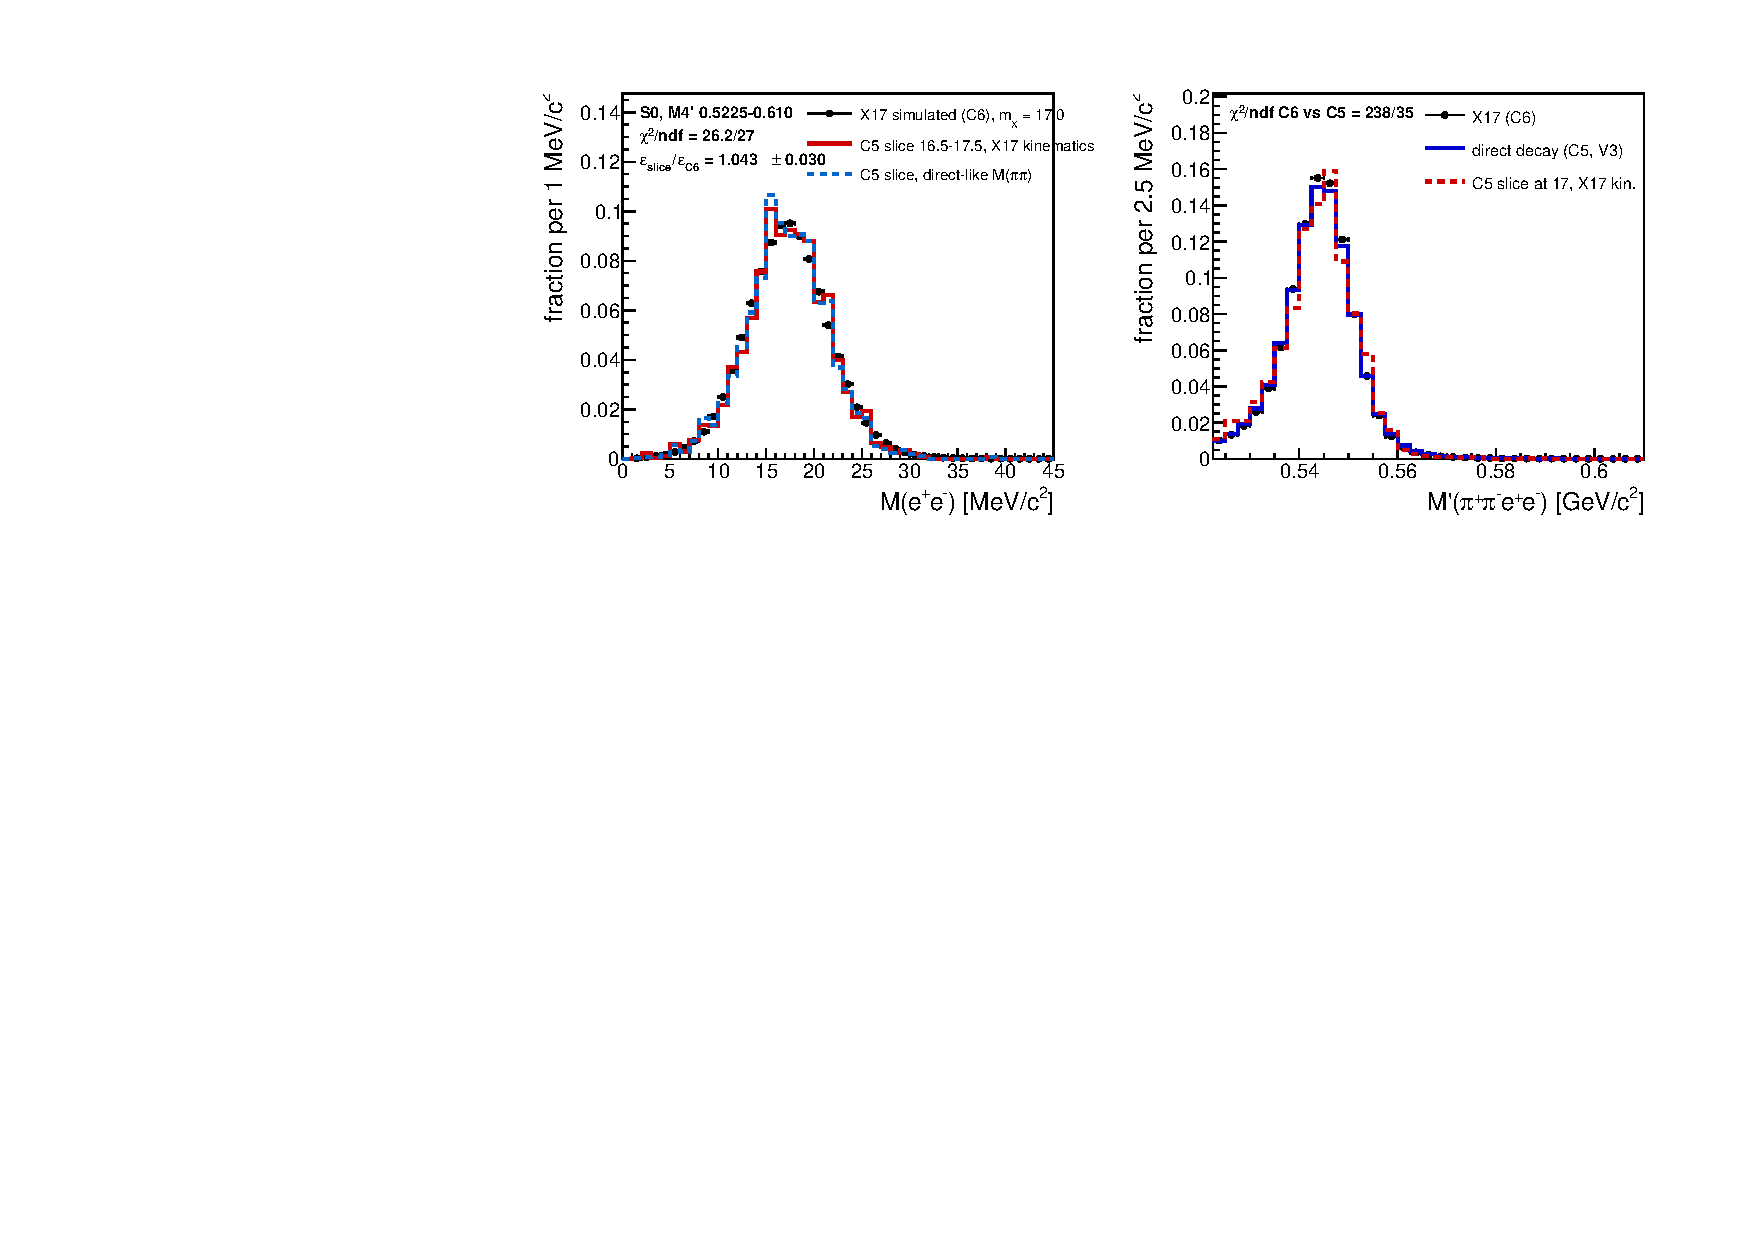
\includegraphics[width=\textwidth]{figs_all/x17ab_line_valid.pdf}\\
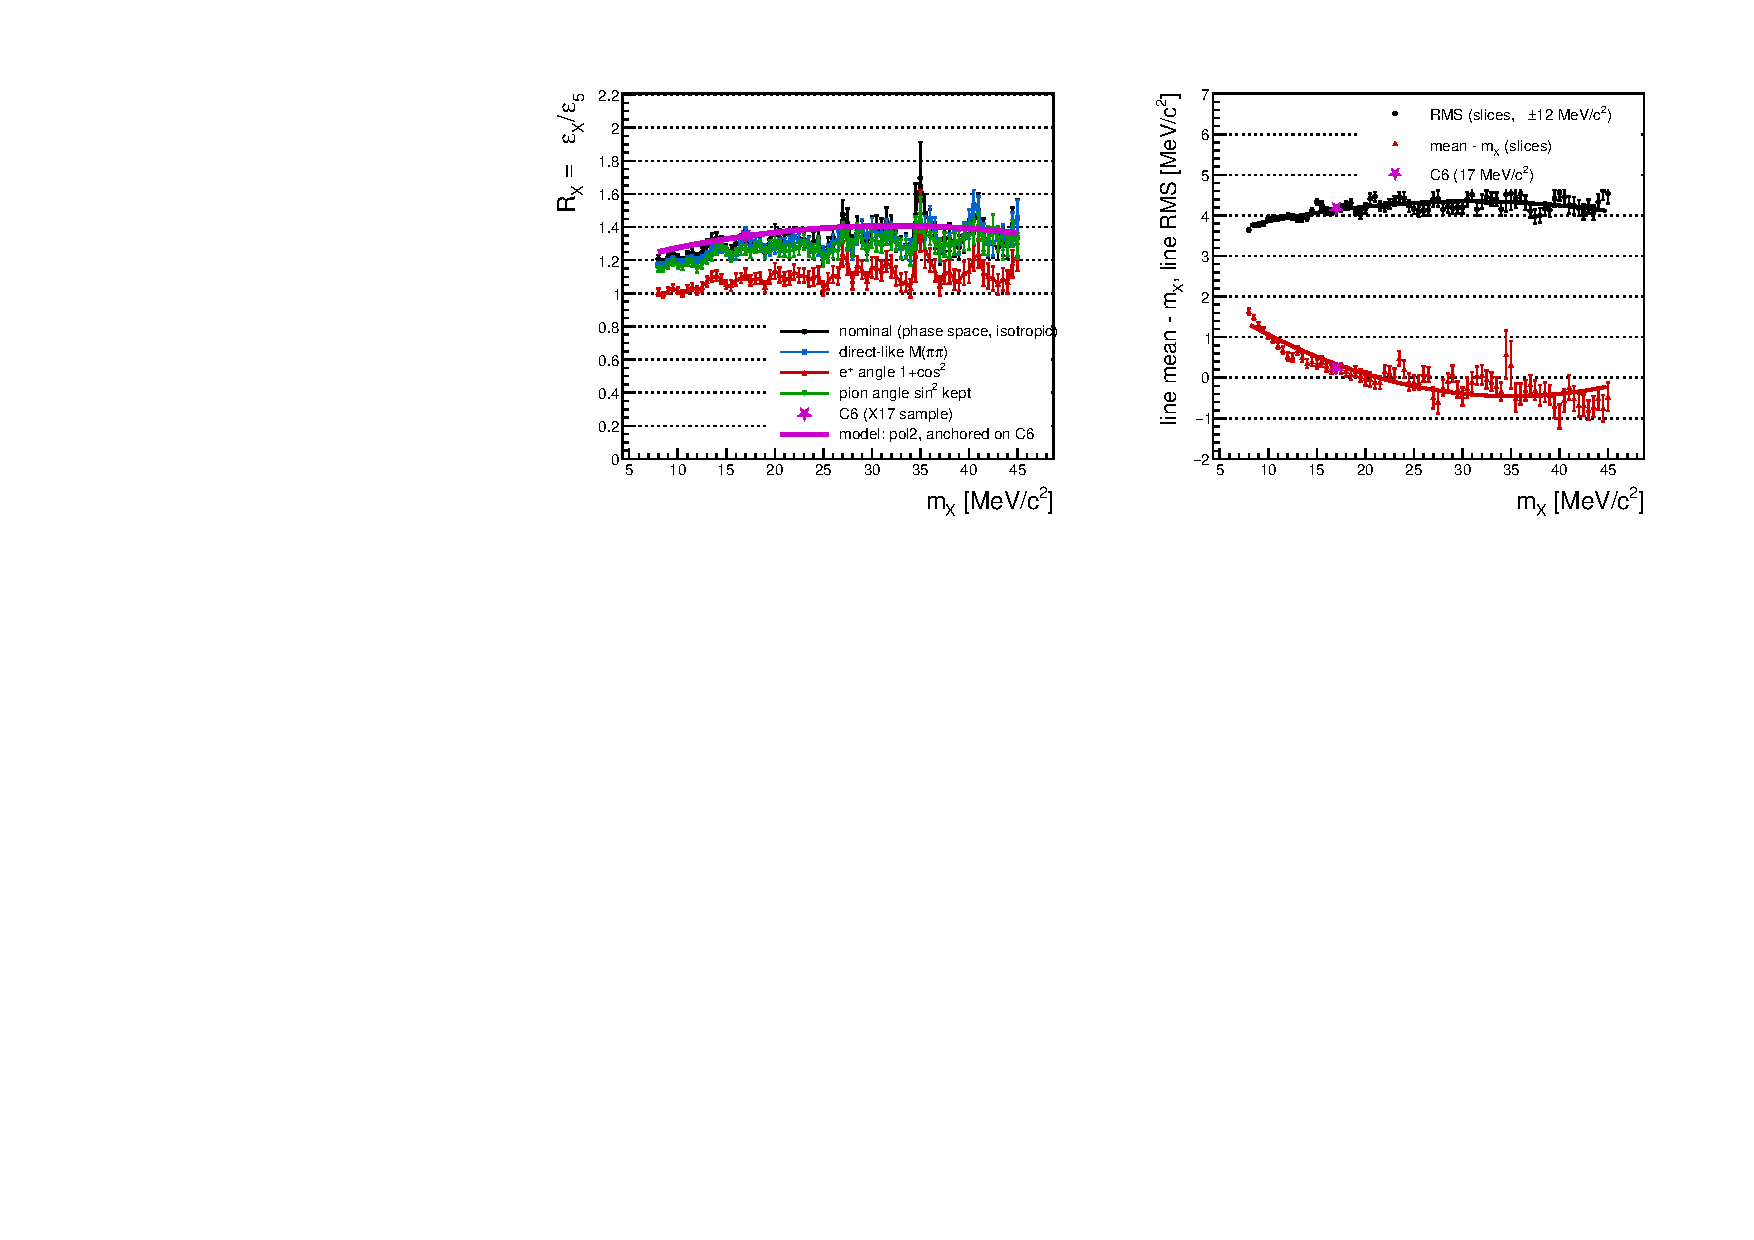
\includegraphics[width=\textwidth]{figs_all/x17ab_line_eff.pdf}
\caption{\textbf{What it shows: an X17 line of any mass can be built from the simulated direct decays; at 17\,\MeVcc the shifted and reweighted direct decays reproduce the line, the \Mfour shape and the efficiency of the simulated X17.}
Selection: simulation only, no data: the SMASH $\eta$ set (every $\eta$ forced into \ppee or $\pipi X17$), mode A, with the nominal cuts S0 (PT3 trigger; event vertex in the target region, $\vz>-160$\,mm; START-free \betanew identification, pions within 3$\sigma$, leptons within 5$\sigma$ with a RICH ring; energy-loss-corrected momenta of all four tracks; both pions used in the event-vertex fit; all stored combinations of an event, isBest $\ge0$) applied to the simulation, simulated \Mfour$'=0.99615\,M_4$ in 0.5225--0.6100\,\GeVcc, all \Mee; X17: simulated $\eta\to\pipi X17$, $X17\to\ee$ at 17.0\,\MeVcc (C6); slices: direct decays $\eta\to\ppee$ (C5, weights V3) with true \Mee within $\pm0.5$\,\MeVcc of the mass.
X17 line for any mass (simulation only, no data; S0, \Mfour$'$ 0.5225--0.610\,\GeVcc; SMASH $\eta$ set, mode A). Top left: reconstructed
\Mee (unit area per \MeVcc) of the simulated X17 (C6, 17.0\,\MeVcc, black), of direct decays with true \Mee 16.5--17.5\,\MeVcc shifted to 17.0 and
reweighted to X17 kinematics (red: phase-space \Mpipi, isotropic $e^+$ and $\pi^+$ angles), and with direct-like \Mpipi (blue dashed). Top right:
\Mfour$'$ of C6, of all direct decays (C5, V3) and of the slice. Bottom left: $R_X$ against $m_X$ for four kinematic assumptions (points, slices
of $\pm0.5$\,\MeVcc), the simulated X17 (star) and the model (pol2 anchored on C6). Bottom right: truncated ($m\pm12$\,\MeVcc) mean $-\,m_X$ and rms
of the slice lines with the pol2 curves that morph the C6 line. No fall-back involved.}
\label{fig:x17line}
\end{figure}

\begin{figure}[H]
\centering
\begin{subfigure}{0.49\textwidth}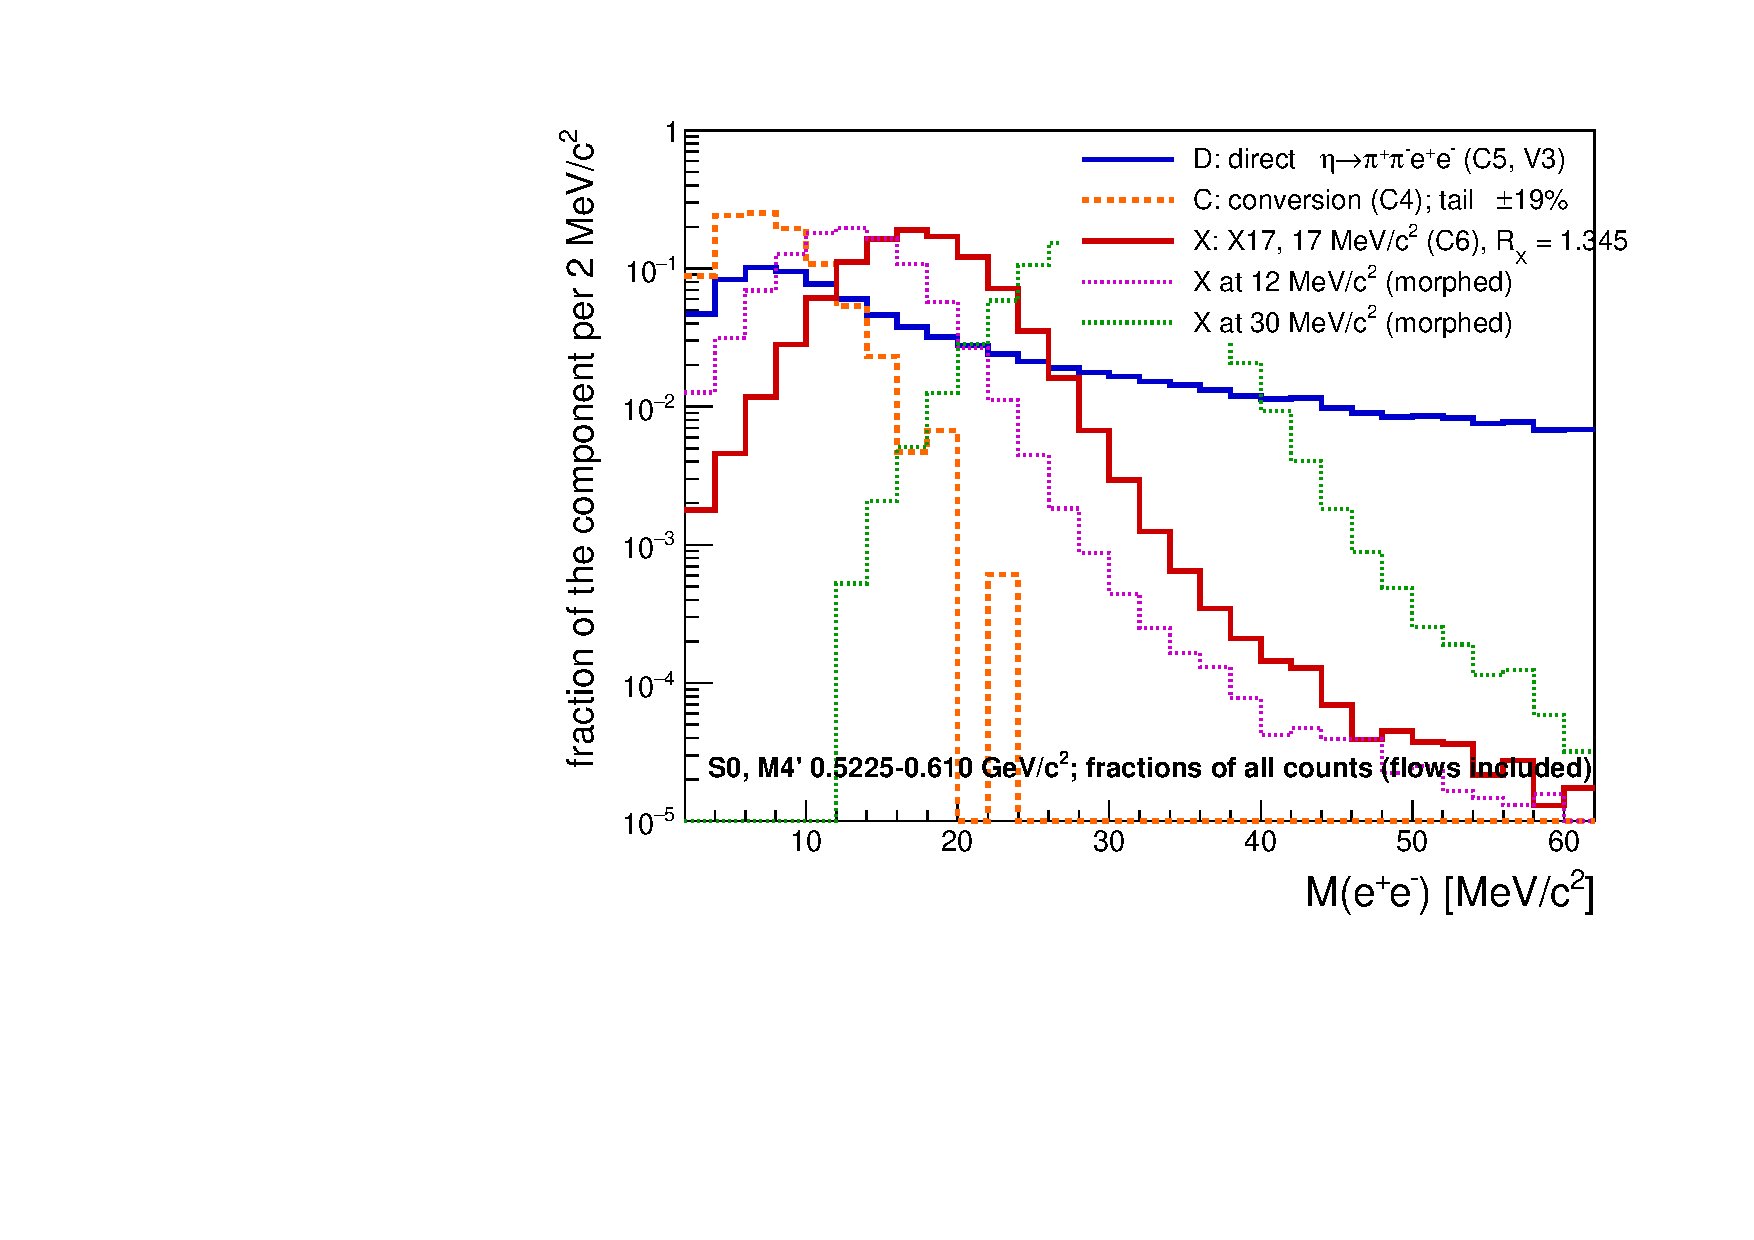
\includegraphics[width=\textwidth]{figs_all/x17ab_model_mee_cnt.pdf}\caption{}\end{subfigure}
\begin{subfigure}{0.49\textwidth}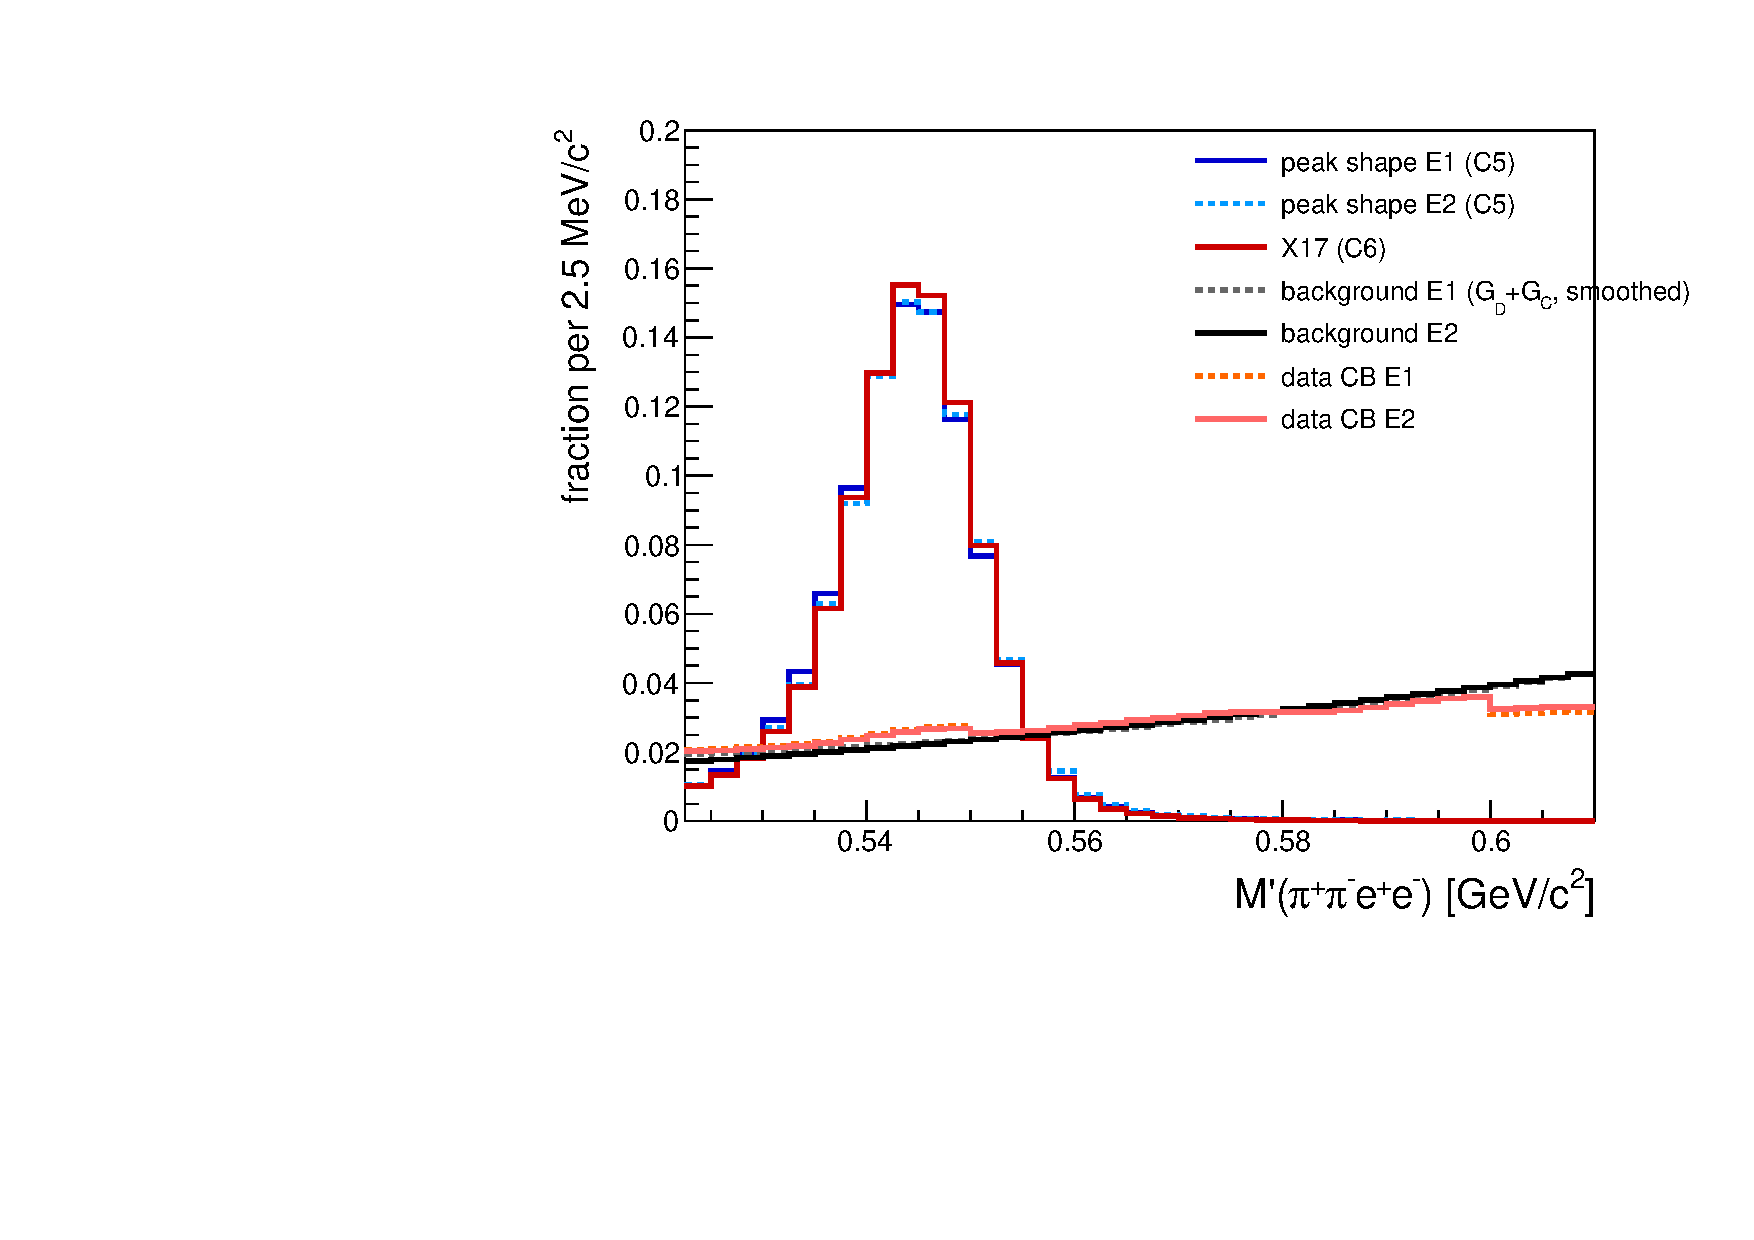
\includegraphics[width=\textwidth]{figs_all/x17ab_model_m4.pdf}\caption{}\end{subfigure}
\caption{\textbf{What it shows: the shapes of the components of the two-dimensional X17 model, in \Mee (a) and in \Mfour (b).}
Selection: SMASH templates (mode A, $w\times$V3, simulated \Mfour$\times0.99615$) and the data CB, both with the nominal cuts S0 (PT3 trigger; event vertex in the target region, $\vz>-160$\,mm; START-free \betanew identification, pions within 3$\sigma$, leptons within 5$\sigma$ with a RICH ring; energy-loss-corrected momenta of all four tracks; both pions used in the event-vertex fit; all stored combinations of an event, isBest $\ge0$), in the plane \Mfour 0.5225--0.6100\,\GeVcc (35 bins of 2.5\,\MeVcc) $\times$ \Mee 2--62\,\MeVcc (30 bins of 2\,\MeVcc); (a) summed over \Mfour 0.5225--0.6100\,\GeVcc; (b) in the classes \Mee 2--10 and 10--62\,\MeVcc; CB $=2\sqrt{N_{++}N_{--}}$ of the like-sign data in 10\,\MeVcc cells of \Mfour, shared over the cells by the like-sign share of each 50\,\MeVcc band.
Shapes of the 2D model. (a) \Mee: fraction of all counts of a component per 2\,\MeVcc bin (flows in the total): direct decays $D$ (C5, V3),
conversions $C$ (C4; tail $\pm19$\,\%), X17 at 17\,\MeVcc (C6, $R_X=1.345$) and at 12 and 30\,\MeVcc (morphed). (b) \Mfour$'$, unit area: $\eta$
peak in E1 and E2 (C5), X17 (C6), background templates (simulated $G_D+G_C$, exp(pol2)) in E1 and E2, data CB per class (like-sign, spread rule;
the steps at 0.55 and 0.60\,\GeVcc are the 50\,\MeVcc band edges). S0; simulation templates at $L=6079.2\,\nbinv$. No fall-back involved.}
\label{fig:x17shapes}
\end{figure}

\subsection{Validation on toys (X-b)}
\label{sec:x17val}
\textbf{Test of the specification}: the 1500 toys of the simulation study (Poisson fluctuations of half B with X17 at BR $=0$, 1, 3, 10,
$30\times10^{-6}$, 300 each, $L=6080.5\,\nbinv$) plus a CB-like component (Poisson(CB$_{\mathrm{data}}$) counts; the fit uses a Poisson event-group
replica of the like-sign counts), templates from half A. \textbf{Own smooth-parent toys}: truth $=$ the model itself with the parameters of a fit to
the half-A Asimov set (300 per BR), because the simulation-study toys share one parent whose heavy entries (one standard-set entry $=55$ expected counts in one
cell) give a Pearson $\chi^2$/ndf of about 29 for any smooth model, even for the mean of 300 toys. Two normalisations: (1) $\mathrm{BR}_1=\hat r\times
2.68\times10^{-4}$; (2) $\mathrm{BR}_2=N_X/s=\hat r\,\hat N_5/N_5^{\mathrm{true}}\times2.68\times10^{-4}$.

\begin{table}[H]
\centering
\caption{X17 toys (BR in $10^{-6}$; BR $=r\times2.68\times10^{-4}$, the simulation convention: a validation, independent of the PDG edition). cov $=$ fraction of toys whose 90\,\% CL$_s$ UL (asymptotic) is $\ge$ the injected BR. Source: x17ab
(\code{x17ab_toys.txt}). Fall-backs fired on the simulation-study toys only; not applied (D30).}
\label{tab:x17toys}
\small
\resizebox{\textwidth}{!}{%
\begin{tabular}{@{}l l l r r r@{}}
\toprule
toys and fit & slope (1) & slope (2) & offset (2) & cov at 10 / 30 & $\chi^2$/ndf \\
\midrule
simulation-study toys + CB, nominal & $0.673\pm0.008$ & $\mathbf{1.038\pm0.012}$ & $-19.5$ & 0.000 / 0.000 & 28.8 \\
\quad same, common offset removed, norm.\ (2) & & & & 1.000 / 0.957 & \\
smooth parent + CB, nominal & $\mathbf{1.024\pm0.015}$ & $\mathbf{1.015\pm0.012}$ & $-0.3$ & \textbf{0.937 / 0.917} & 1.01 \\
three-class truth, nominal fit & $1.056\pm0.016$ & $0.991\pm0.012$ & $-1.0$ & 0.937 / 0.913 & 1.18 \\
three-class truth, fit without \Mee dependence & 0.910 & 0.994 & $-8.4$ & 0.393 / 0.333 & 1.24 \\
\bottomrule
\end{tabular}}
\end{table}

The simulation-study toys fit $\hat N_5=11\,168$ at BR $=0$ against a true 7200 ($+55$\,\%); the parent check gives $+51$\,\% for the mean of the 300
BR $=0$ toys (half B) and $-58$\,\% for the half-A Asimov set, i.e.\ opposite offsets of about $18\times10^{-6}$: the size of the simulation-background
noise projected on X17 (the simulation study found 11.8--$23\times10^{-6}$ for counting). This is a property of the parent, not of the method; on the
smooth toys the slope, coverage (pulls: mean $-0.09$, rms 0.98) and the median UL at BR $=0$ ($9.2\times10^{-6}$, $\aEta=1$, simulation background) are
as expected. \textbf{Asymptotic against toy CL$_s$} (8 values of $r$, 1000 toys per value and hypothesis): ratios 0.967--1.046 on seven data sets
(Table~\ref{tab:x17toycls}); one simulation-study toy with $\hat r$ at $-4.6\sigma$ has CL$_b=0$ and an undefined toy CL$_s$. The asymptotic limit stays
primary (rule: toys primary if they differ by more than 10\,\%).

\begin{table}[H]
\centering
\caption{Asymptotic against toy CL$_s$ upper limits ($10^{-6}$; simulation convention $r\times2.68\times10^{-4}$, a validation). Source: x17ab (\code{x17ab_toycls.txt}). No fall-back involved.}
\label{tab:x17toycls}
\small
\resizebox{\textwidth}{!}{\tabin{x17ab_toycls.tex}}
\end{table}

\begin{figure}[!htbp]
\centering
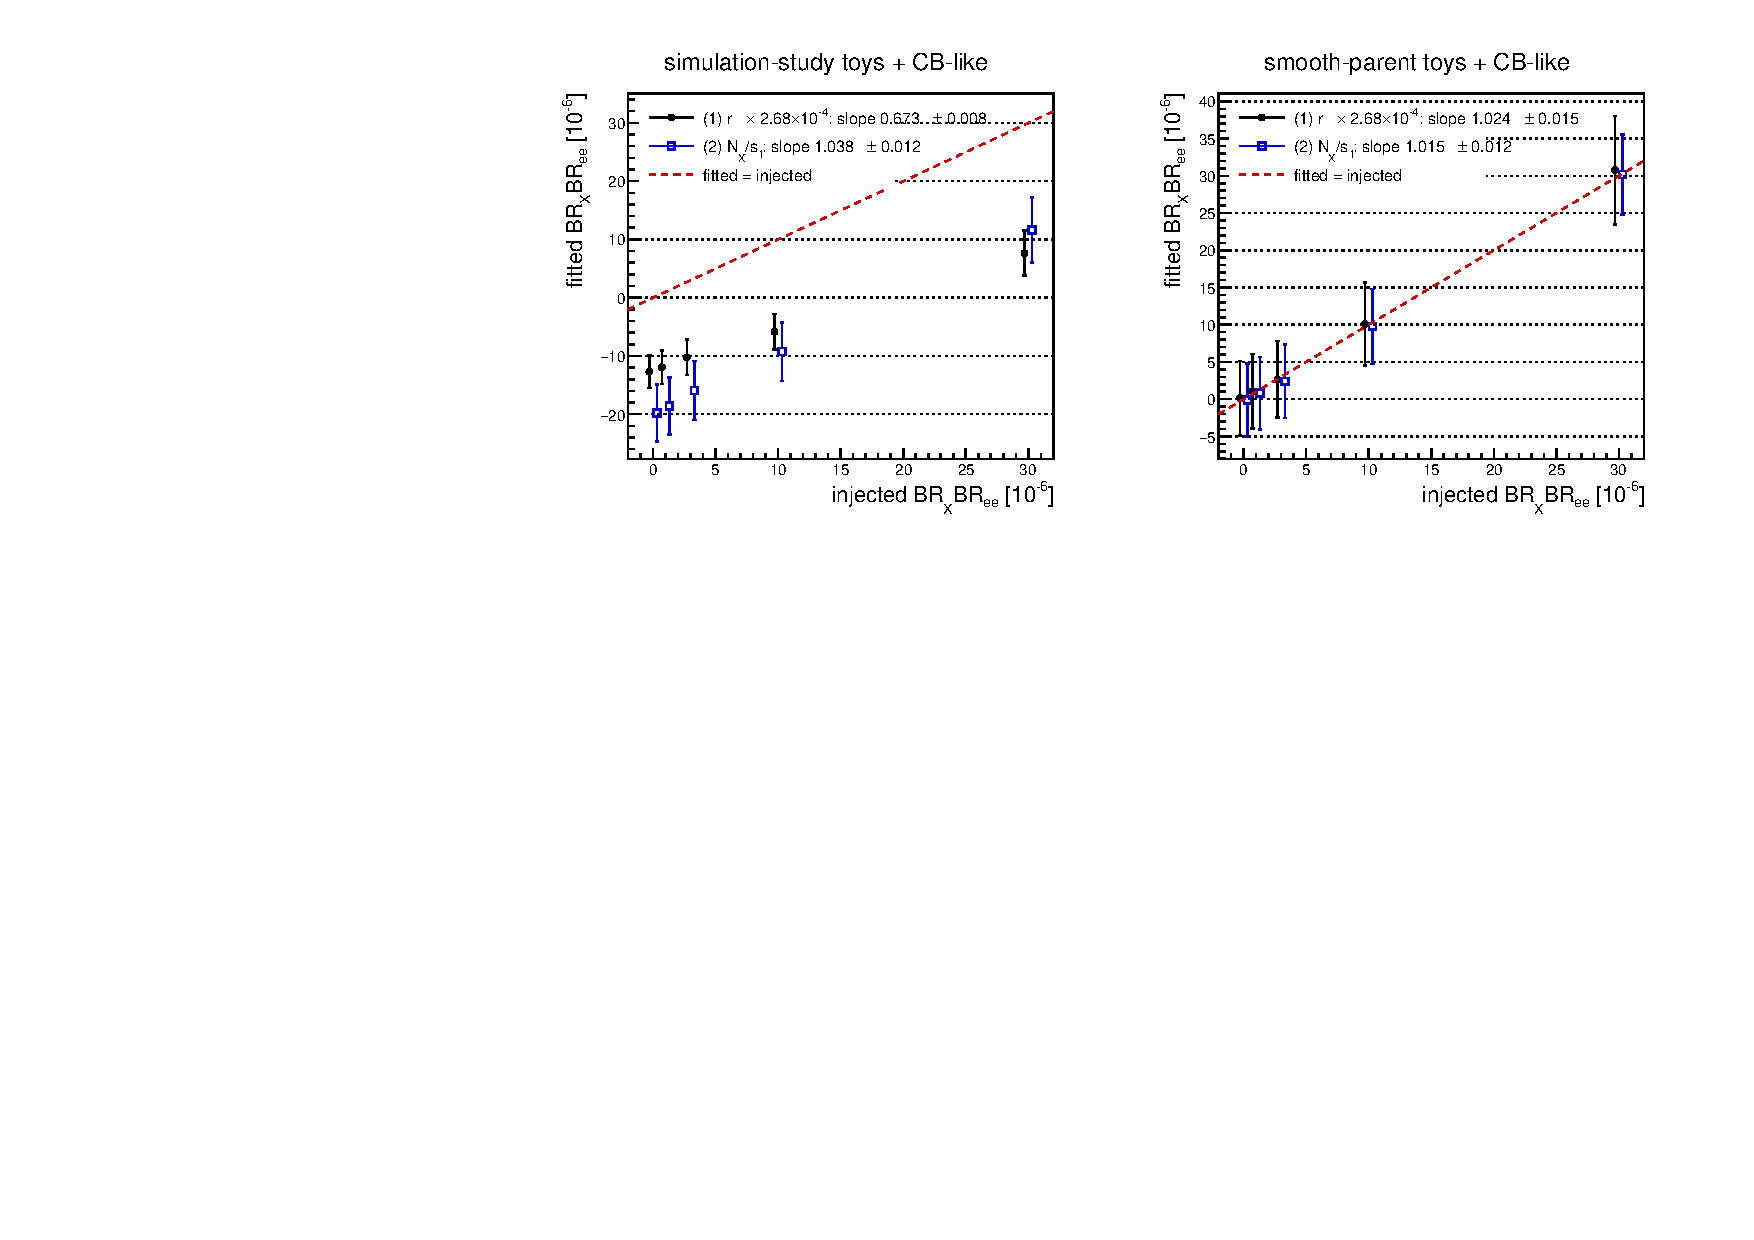
\includegraphics[width=\textwidth]{figs_all/x17ab_toys_lin.pdf}\\
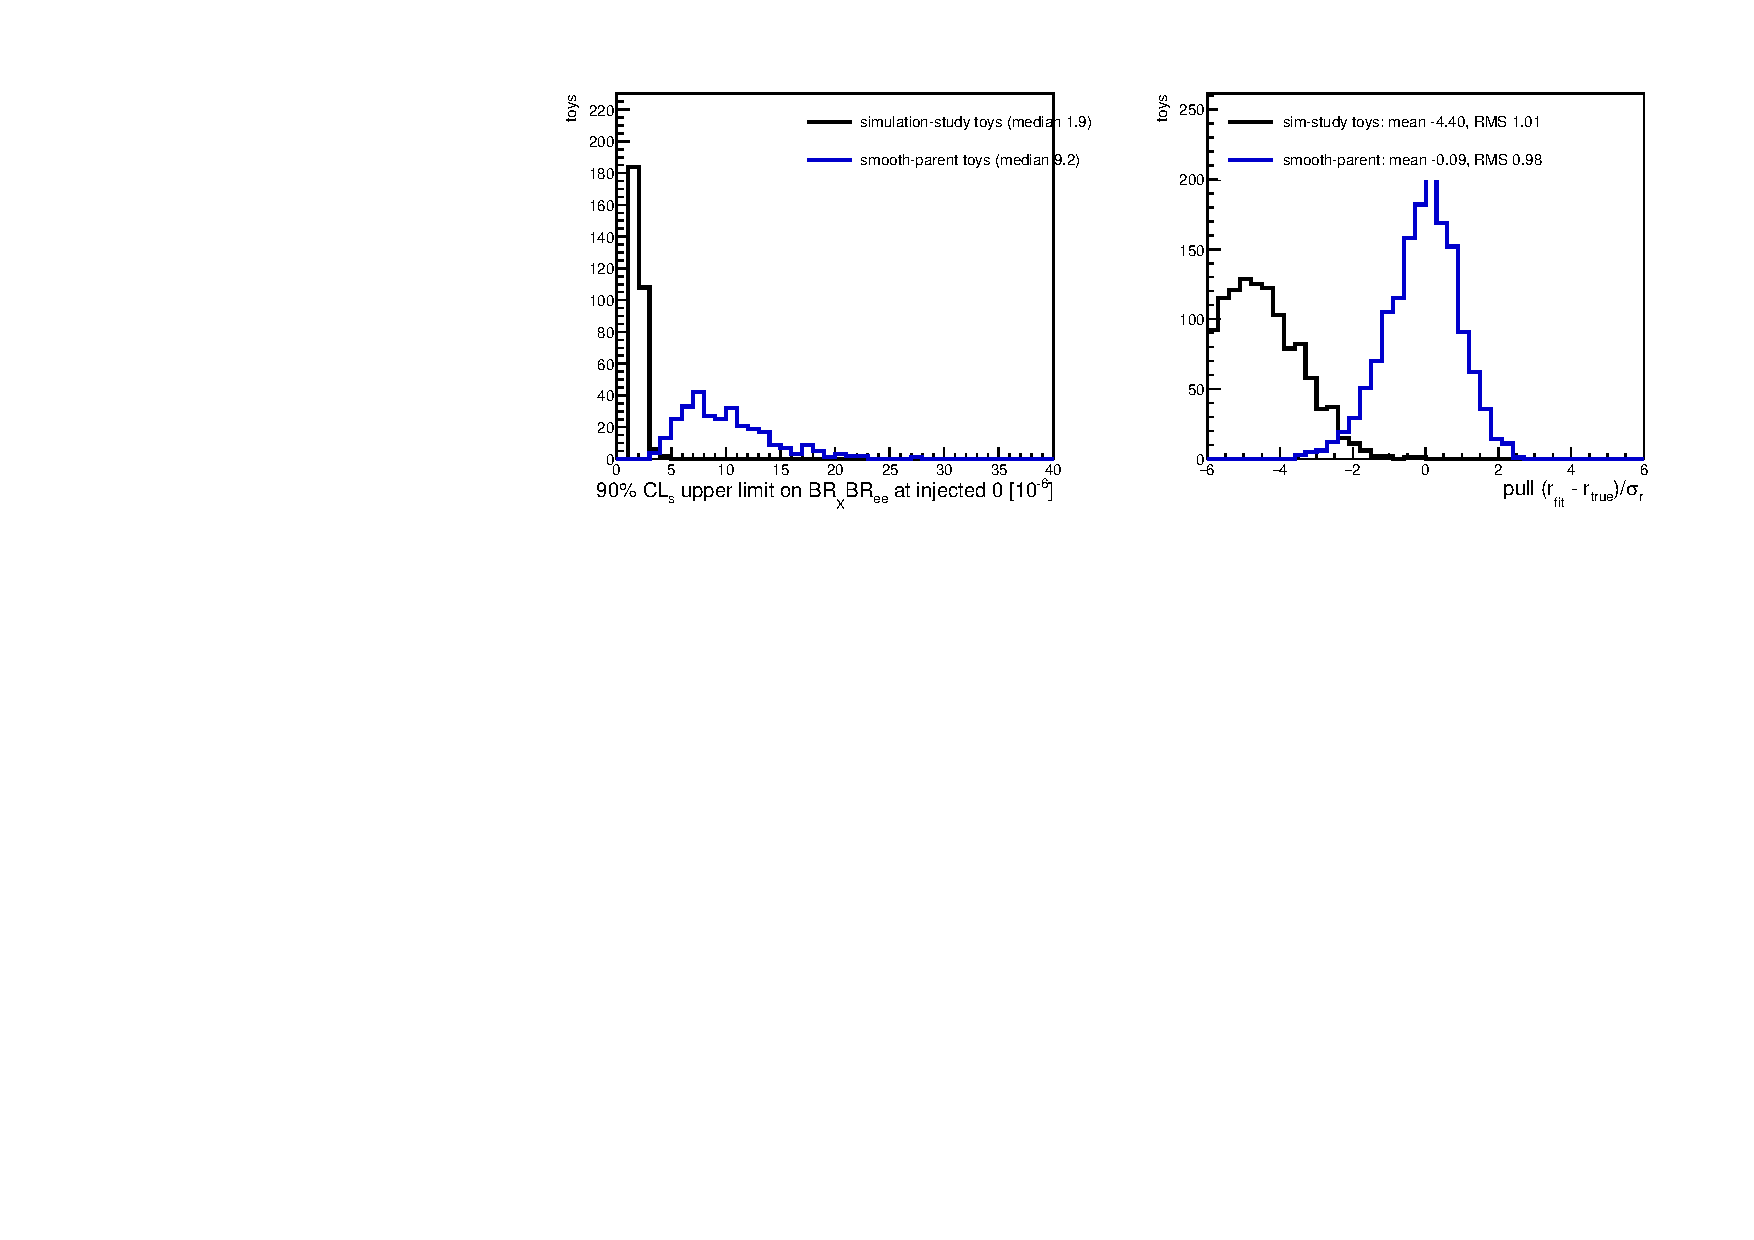
\includegraphics[width=\textwidth]{figs_all/x17ab_toys_ul.pdf}
\caption{\textbf{What it shows: on smooth-parent toys the X17 fit returns the injected branching ratio with correct pulls; on the toys of the simulation study the heavy simulated entries of their common parent shift the results by a common offset.}
Selection: simulation only, no data counts. Left: the 1500 toys of the simulation study, Poisson fluctuations of one half of SMASH (odd event groups; $\eta$ signal and physical background, $T_1+T_2$, with X17 injected at BR $=0$, 1, 3, 10 and $30\times10^{-6}$, 300 toys each) at $L=6080.5\,\nbinv$, with the nominal cuts S0 (PT3 trigger; event vertex in the target region, $\vz>-160$\,mm; START-free \betanew identification, pions within 3$\sigma$, leptons within 5$\sigma$ with a RICH ring; energy-loss-corrected momenta of all four tracks; both pions used in the event-vertex fit; all stored combinations of an event, isBest $\ge0$) applied to the simulation, simulated \Mfour without mass transfer in 0.5230--0.6080\,\GeVcc (34 bins) $\times$ \Mee 2--62\,\MeVcc (30 bins), plus Poisson counts of the data CB; the fit takes as CB a Poisson event-group replica of the like-sign data and its templates from the other half (even event groups). Right: smooth-parent toys on the same grid, truth $=$ the model fitted to the Asimov set of the template half, 300 per BR, plus Poisson counts of the CB.
Validation of the X17 fit (nominal model; BR in the simulation convention $r\times2.68\times10^{-4}$, independent of the PDG edition). Top: fitted against injected \BRX in the two normalisations, (1) $r\times2.68\times10^{-4}$ and
(2) $N_X/s$; bars $=$ rms of 300 toys; left the 1500 toys of the simulation study plus a CB-like component (the common offset and the $N_5$ bias come
from the heavy-entry structure of the simulated parent), right smooth-parent toys plus CB. Bottom: 90\,\% CL$_s$ limits at injected BR $=0$ (left) and
pulls $(r_{\mathrm{fit}}-r_{\mathrm{true}})/\sigma_r$ (right); black: simulation-study toys, blue: smooth-parent toys. Fall-backs fired on the simulation-study toys only; not applied (D30).}
\label{fig:x17toys}
\end{figure}

\textbf{Pre-data projection} (simulation Asimov set: $\aEta=0.40$, background $1.35\times$ SMASH, data CB; not a result; BR in the PDG 2020 units of the frozen
procedure, $\times1.030$ for PDG 2026, e.g.\ 2.91 instead of 2.83 at 17\,\MeVcc): expected 90\,\% CL$_s$ at
17\,\MeVcc $2.83\times10^{-5}$ ($\pm1\sigma$: 1.76--5.07, $\pm2\sigma$: 1.21--10.7 in $10^{-5}$), 424 X17 counts; statistical error of $N_5$ 21.5\,\%;
median 5.29 / 3.19 / 2.83 / 2.42 / 1.88 / 1.49 / 1.07 $\times10^{-5}$ at 10 / 15 / 17 / 20 / 25 / 30 / 40\,\MeVcc. The model choices tested on the
projection (\code{x17ab_nuis.txt}) give: line width $\pm10$\,\% UL $\times1.10/0.90$; $e^+$ angle $1+\cos^2$ $\times1.20$; direct-decay templates V2
$\times1.19$ ($\varepsilon_5$ of V2 is 16\,\% higher); three background classes: bias $-3.0\times10^{-6}$, UL $\times0.68$, $N_5$ $+22$\,\%; exp(pol3):
$+1.0\times10^{-6}$, $\times0.75$; replica spread of $\hat r$ over 20 C4 replicas $2.1\times10^{-6}$; half spread of $N_5$ over the background and CB
variants 10.9\,\%. The X-b acceptance criteria: slope $1\pm0.05$ in normalisation (2) on the simulation-study toys ($1.038\pm0.012$, PASS),
normalisation (1) FAIL there ($0.673$, $N_5$ $+55$\,\% from the parent) but PASS on the smooth toys (1.024); 90\,\% coverage $\ge0.88$ PASS on the
smooth toys and on the three-class stress test, FAIL on the raw simulation-study toys (common offset) and PASS after removing it (diagnostic).
The fall-backs ``Pearson $\chi^2>1.5$'' and ``slope off by $>5$\,\%'' fired on the simulation-study toys only (a property of their parent; not
applied, the decision was left to X-c for the data). \flag{Deviation (D30): on the toys the specification prescribes, normalisation (1) fails
(slope 0.673, coverage 0.000), and the fall-back would make normalisation (2) primary ($3.29\times10^{-5}$ observed, PDG 2026); (1) was kept on the
evidence of the smooth-parent toys, which were built after that test. The headline therefore gives the range 3.16--$3.29\times10^{-5}$ (PDG 2026; 3.06--3.28 with PDG 2020). Approved by the analyst on 15 November
2026: (1) primary, (2) quoted next to it.}

\subsection{The freeze (X-c)}
\label{sec:x17freeze}
\textbf{Side-band fit.} The model (copied into \code{x17c_model.h} with four flagged additions: normalisations (2)/(3) decoupled from the fitted \aEta,
a log-normal X17 yield nuisance, the line width ($\pm10$\,\%) and \Mee scale ($\pm2$\,\%) as likelihood nuisances, and a variance factor) was fitted
with $r=0$ to the 770 side-band cells (197\,752 counts): Pearson $\chi^2/\mathrm{ndf}=749.0/730=1.026$ (E1 99.1 for 140 cells, E2 650.0 for 630; largest
row 49.3/35 at 30--32\,\MeVcc); $N_5=3380\pm686$ (20.3\,\%), $N_4=1803\pm429$, $\kEone=1.04\pm0.50$, $\kEtwo=1.000\pm0.050$, $\aEta=0.265\pm0.142$, $g=1.40\pm0.93$;
residual near $m_\eta$ (0.5425--0.5525): E1 $-41\pm119$, E2 $-76\pm76$ counts. \textbf{Variance factor}: the event-group dispersion for X17-like weights
on the side-band cells is $\phi=1.017$--1.030 (lines at 8--44\,\MeVcc); frozen $q$-scale $=1.0299$ ($\times1.021$ on the expected median).
\textbf{Masked-row prediction} (enters only the expectation and the counting check, not the observed 2D limit, where $n_j$ is free): $n_j=
\mathrm{sim}_j\times\exp(\mathrm{pol2})$ fitted to the 22 side-band rows; ratio $n_j/\mathrm{sim}_j$ 1.41 (12--14\,\MeVcc) to 1.27 (26--28); 57\,572
predicted counts in the 8 masked rows.

\begin{table}[H]
\centering
\caption{Frozen priors of the X17 likelihood (X-c). The \aEta prior is the WP5 total error $\times1.61$ ($\chi^2$ rule) $\oplus$ the shift of the
quadratic variant (0.149), because WP5 is a cross-check; $g$ the same way. $s_X(1)=0.247$: $R_X$ with direct-like \Mpipi 0.021, generator pion angle
0.041, slice/C6 validation 0.043, BR$_{\mathrm{dir}}$ 0.041, $N_5$ bias 0.153, direct shape (V2) 0.158, peak width 0.078, mass scale 0.029.
Source: x17c (\code{x17c_nuisances.tex}). Frozen values; in the PDG 2026 rerun (D25) the BR$_{\mathrm{dir}}$ part is 0.058 and $s_X(1)=0.250$
(\code{x17c_nuisances_pdg26.tex}). No fall-back involved.}
\label{tab:x17prior}
\small
\resizebox{\textwidth}{!}{\tabin{x17c_nuisances.tex}}
\end{table}

\textbf{Three normalisations of the X17 yield}: (1) $r\,N_5\,R_X$ with $N_5$ fitted (primary); (2) $r\,\aEta\,N_5^{\mathrm{ref}}R_X$ with the WP5
$\aEta=0.382$; (3) the same with the peak scale $\aP=\Ypeak(\mathrm{WP5})/\Ypeak(\mathrm{sim})=5045/12165=0.415\pm0.109$. \flag{The \aEta prior and
\aP come from WP5 (a cross-check); WP6, the main peak result, was not available at the freeze. With WP6's 5088, \aP would be 0.418 and UL (3) about
1\,\% lower. The frozen values are kept.}

\begin{table}[H]
\centering
\caption{Expected 90\,\% CL$_s$ upper limits ($\times10^{5}$), frozen before unblinding. Background-only Asimov set of the data side-band fit (no data
of \Mee 12--28\,\MeVcc used) and background-only toys; S0, isBest $\ge0$, X2D, $L=6079.2\,\nbinv$, 2D likelihood, $\tilde q_r$. Frozen choice: toy
median and bands at the quoted masses, the Asimov curve against $m_X$. Converted to PDG 2026 (D25): the Asimov set rerun with
BR$_{\mathrm{dir}}=2.76\times10^{-4}$ and its PDG 2026 uncertainty, the toys $\times2.76/2.68\times k$ ($k=1.0011$--1.0013), (2) $\times1.00436$,
(3) $\times1.0224$. Source: x17c (\code{x17c_expected.tex}, PDG 2020, frozen), converted in \code{x17c_expected_pdg26.tex}. No fall-back involved.}
\label{tab:x17exp}
\small
\resizebox{\textwidth}{!}{\tabin{x17c_expected_pdg26.tex}}
\end{table}

\textbf{Checks of the frozen fit.} Background-only toys: $\hat r/\sigma$ mean $-0.14$, rms 0.94 (17\,\MeVcc); 100\,\% converged. Injection at 17\,\MeVcc in
normalisation (1): mean $\hat r$/injected 1.106 / 1.059 / 1.061 at 1 / 3 / $6\times10^{-5}$, slope after the background-only offset 1.0385; coverage of the
90\,\% CL$_s$ UL 0.990 / 0.888 / $0.876\pm0.015$ (marginal at $6\times10^{-5}$, far above the expected limit; there the Hessian error of $\hat r$ is too small,
pull rms 1.2, but the limit uses $\tilde q$). Toy against asymptotic CL$_s$ on the Asimov set at 17\,\MeVcc: UL $2.91\times10^{-5}$ against $2.84\times10^{-5}$
(PDG 2026; ratio 1.023). Template statistics on the Asimov set: $\sigma(\hat r)=1.19\times10^{-5}$ (PDG 2026); $\hat r$ rms over 50 CB replicas $1.1\times10^{-6}$, over 50 C4
replicas $1.4\times10^{-6}$. Single choices on the expected median at 17\,\MeVcc (nominal $2.84\times10^{-5}$ with PDG 2026, 2.76 in the frozen PDG 2020 units): without the $q$-scale $\times0.979$, without
$s_X$ $\times0.953$, \aEta and $g$ fixed $\times0.966$, line width fixed at $\times1.10$ / 0.90 $\times1.097$ / 0.907, $e^+$ angle $1+\cos^2$ $\times1.198$;
variants with their own side-band fit: exp(pol3) $\times0.784$, three classes $\times0.745$, no \Mee dependence $\times1.038$, V2 $\times1.186$. The
frozen expected median (2.84 with PDG 2026) is within 3\,\% of the pre-data projection (2.91). \textbf{Counting window X17c} (frozen prediction): $B_{\mathrm{pred}}=6311.7$
counts (CB 212.3), $\sigma_B=1195.5$ counts (the largest deviation among the reference choices of the masked rows); $s_1=2.0954\times10^7$ raw counts per unit
BR at $\aEta=1$. No fall-back fired.

\begin{figure}[!htbp]
\centering
\begin{subfigure}{0.49\textwidth}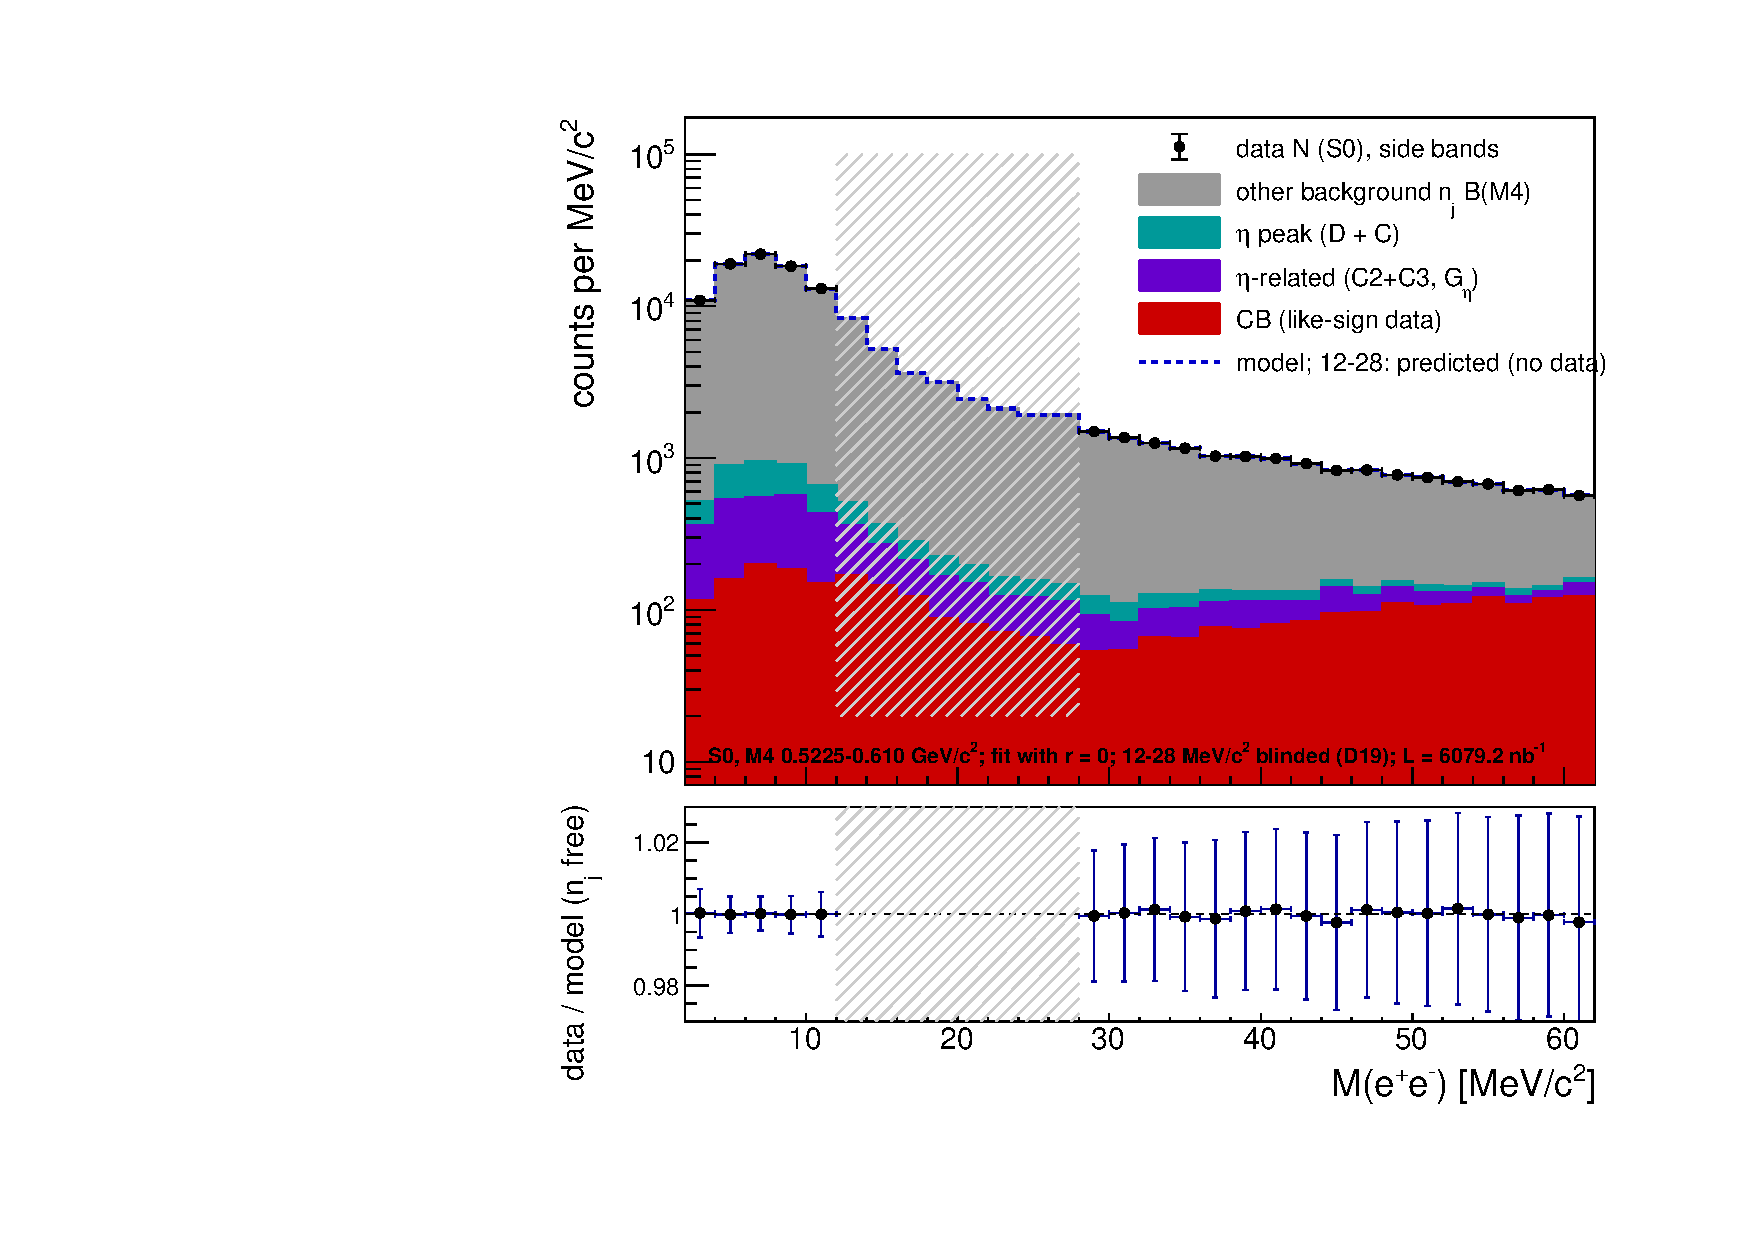
\includegraphics[width=\textwidth]{figs_all/x17c_sb_mee_cnt.pdf}\caption{}\end{subfigure}
\begin{subfigure}{0.49\textwidth}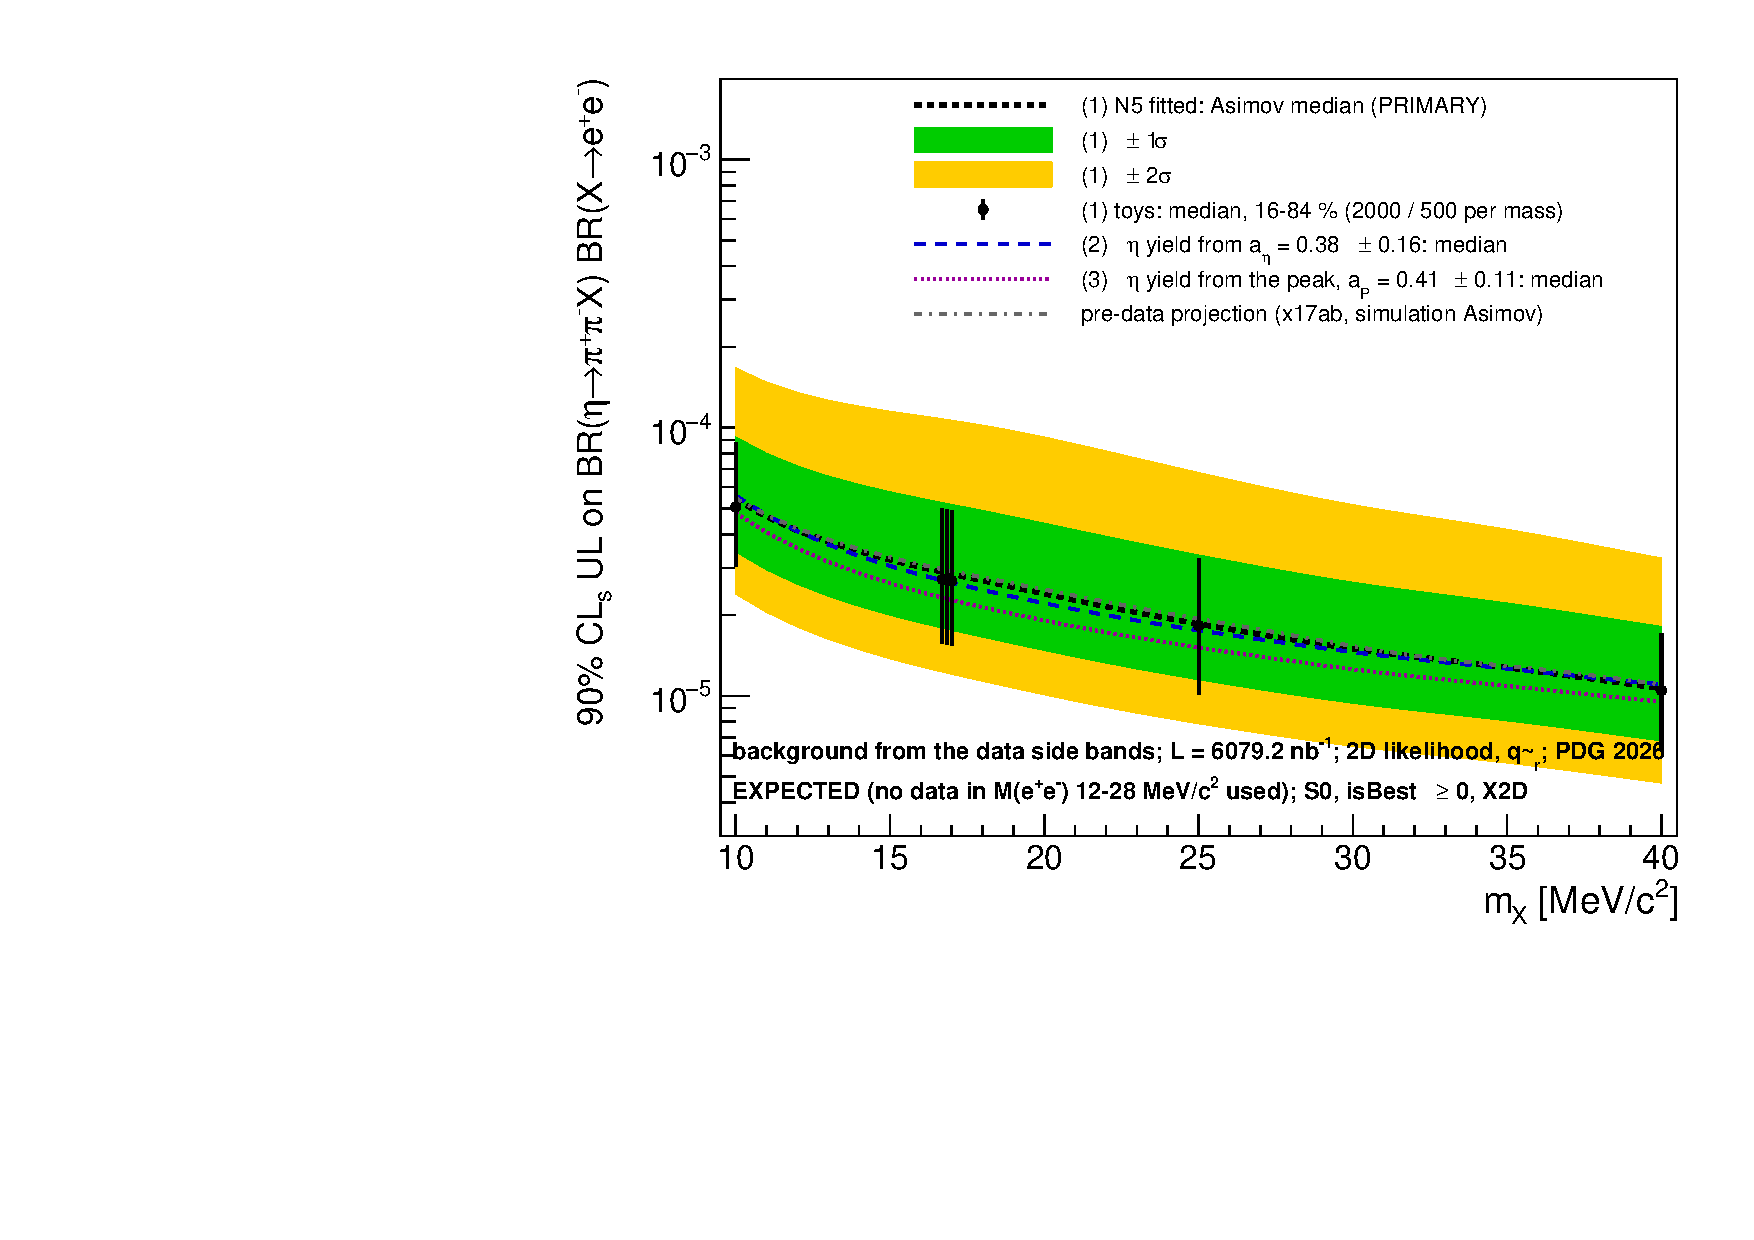
\includegraphics[width=\textwidth]{figs_all/x17c_expected_pdg26.pdf}\caption{}\end{subfigure}
\caption{\textbf{What it shows: before the hidden \Mee range was opened, the model without X17, fitted to the \Mee side bands alone, gave the predicted background in 12--28\,\MeVcc and the expected limit against $m_X$.}
Selection: (a) data at $L=6079.2\,\nbinv$ with the nominal cuts S0 (PT3 trigger; event vertex in the target region, $\vz>-160$\,mm; START-free \betanew identification, pions within 3$\sigma$, leptons within 5$\sigma$ with a RICH ring; energy-loss-corrected momenta of all four tracks; both pions used in the event-vertex fit; all stored combinations of an event, isBest $\ge0$), \Mfour 0.5225--0.6100\,\GeVcc (35 bins of 2.5\,\MeVcc), \Mee side bands 2--12 and 28--62\,\MeVcc in 2\,\MeVcc bins (\Mee 12--28\,\MeVcc hidden until the procedure was frozen); CB of the like-sign data with the same cuts (10\,\MeVcc cells of \Mfour, shared over the \Mee bins by the like-sign share of each 50\,\MeVcc band), its factor fitted within $1\pm0.5$ for \Mee$<10$\,\MeVcc and $1\pm0.05$ above; the other templates from SMASH with the same cuts (mode A, $w\times$V3, simulated \Mfour$\times0.99615$). (b) Expected limits from the background-only Asimov set and toys of that side-band fit, in the full plane \Mfour 0.5225--0.6100\,\GeVcc $\times$ \Mee 2--62\,\MeVcc.
The freeze. (a) Data $N$ per \MeVcc (black) in the side bands \Mee 2--12 and 28--62\,\MeVcc, S0, isBest $\ge0$, \Mfour 0.5225--0.610\,\GeVcc;
stacked: the model fitted with $r=0$ to the side bands only (CB from like-sign data red, $\eta$-related terms violet, $\eta$ peak $D+C$ cyan, other
background $n_jB$ grey); hatched: 12--28\,\MeVcc, blinded, where the dashed line is the \emph{predicted} background; lower panel data/model (1 by
construction, $n_j$ free per row). (b) Expected 90\,\% CL$_s$ upper limit on \BRX against $m_X$ (PDG 2026, D25): normalisation (1) Asimov median (dashed), $\pm1\sigma$
(green), $\pm2\sigma$ (yellow); points: toy median and 16--84\,\% (2000 toys at 16.7/16.85/17.0, 500 at 10/25/40); (2) blue dashed; (3) magenta dotted;
pre-data projection grey dash-dotted. $L=6079.2\,\nbinv$. No fall-back involved.}
\label{fig:x17freeze}
\end{figure}

\subsection{Unblinding (X-d)}
\label{sec:x17d}
\textbf{Full data and fit.} Side-band cells from \code{hists_v1.root} (mask intact), the 8 masked rows from the sealed file (its side-band cells are
identical, largest difference 0): 255\,331 counts in 1050 cells, 57\,579 of them newly opened. The frozen side-band fit was rerun first and reproduces
$B_{\mathrm{pred}}=6311.7$ and the Asimov median $2.7589\times10^{-5}$ (frozen $2.7590$; both in the PDG 2020 units of the freeze, a reproduction check). The frozen model fitted to all cells: Pearson $\chi^2/\mathrm{ndf}=
994.9/1002=0.993$ ($r=0$) and $994.7/1001$ ($r$ free); unblinded cells alone 245.0 for 280 cells; the fall-back ($\chi^2/\mathrm{ndf}>1.5$) did not fire,
$q$-scale stays 1.0299. Parameters ($r=0$): $N_5=3659\pm503$ (13.7\,\%), $N_4=1648\pm383$, $\aEta=0.253\pm0.138$ (prior $0.382\pm0.165$), $g=1.48\pm0.93$,
$\kEtwo=0.998\pm0.050$. Peak-band residual (\Mfour 0.5325--0.5575) of the $r=0$ fit: $+44\pm117$ counts in 12--28\,\MeVcc ($+0.38\sigma$), $+71\pm95$ in
14--26\,\MeVcc ($+0.74\sigma$); per row $|$pull$|\le0.5$ in 12--28; the largest pull anywhere is $-2.05$ at 44--46\,\MeVcc (side band). The background of the
unblinded rows agrees with the frozen prediction in sum (53\,126 fitted vs 53\,132 predicted) but not row by row (0.81--1.10, following the fluctuations of
the simulated reference rows); the observed limit does not use the prediction.

\begin{table}[H]
\centering
\caption{Spec.\ Table~D1: observed 90\,\% CL$_s$ upper limits on \BRX at three masses and in the three normalisations of the frozen procedure: (1) $r\times
2.76\times10^{-4}$ (PDG 2026, D25: the frozen code rerun with only BR$_{\mathrm{dir}}$ changed; the frozen PDG 2020 value gives $3.06\times10^{-5}$ at
17\,\MeVcc) with $N_5$ fitted (primary; the specification's fall-back would make (2) primary; D30, approved: (1) primary, (2) quoted next to it); (2) $N_X/(\aEta s_{\mathrm{X2D}})$; (3) relative to the measured $\eta$ peak. Expected $=$ frozen
background-only toys (median and 68\,\% band), computed before the \Mee 12--28\,\MeVcc rows were opened. $N_X^{\mathrm{UL}}$: direct 90\,\% CL$_s$ limit on the
number of X17 counts (raw counts; 398 after $\times64/63$ at 17\,\MeVcc), the same in all normalisations. Data S0, isBest $\ge0$, X2D, $L=6079.2\,\nbinv$,
isotropic $e^+$ angle. Template statistics (MC: CB $\oplus$ C4 replicas, 11\,\% in (1)) and the $1+\cos^2$ hypothesis are quoted separately. Source:
x17d with the corrections of the verifier vx (\code{x17d_D1.txt}), converted to PDG 2026 in \code{x17d_D1_pdg26.txt} ((2) $\times1.00436$ and
(3) $\times1.0224$ through the PDG 2026 BR$(\eta\to\pipi\piz)$ in their $\eta$ scales; toy columns $\times1.0299\,k$). No fall-back fired on the
data (D30, approved: normalisation (1) primary, (2) quoted next to it).}
\label{tab:D1}
\footnotesize
\resizebox{\textwidth}{!}{\tabin{x17d_D1_pdg26.tex}}
\end{table}

\begin{table}[H]
\centering
\caption{Observed limits against $m_X$ (selection of the 38 masses; \code{x17d_scan.txt}). $\hat r$ with its Hessian error (a fit result, not a
measurement; the profile is about 40\,\% wider at the limit). Last columns: the frozen Asimov median and normalisation (1) with the $e^+$ angle
$1+\cos^2\theta$. PDG 2026 (D25): UL (1), $\hat r$, the frozen median and the $1+\cos^2$ column rerun with BR$_{\mathrm{dir}}=2.76\times10^{-4}$,
(2) $\times1.00436$, (3) $\times1.0224$ (\code{x17d_scan_pdg26.txt}; the PDG 2020 values are in \code{x17d_scan.txt}). No fall-back fired on the
data (D30, approved: normalisation (1) primary, (2) quoted next to it).}
\label{tab:x17scan}
\small
\resizebox{\textwidth}{!}{\tabin{x17d_scan_pdg26.tex}}
\par\smallskip\footnotesize Rows after the first in units of $10^{-5}$.
\end{table}

\textbf{Further results.} Toy CL$_s$ on the data (9 values of $r$ at 0.55--1.8 $\times$ the asymptotic UL, 1000 toys per point and hypothesis): ratio toy/asymptotic
0.958 / 1.002 / 0.983 in (1) at 16.7 / 16.85 / 17.0\,\MeVcc, 1.008--1.041 in (2), 1.011--1.018 in (3); all within 10\,\%, so the asymptotic limit stays
primary; CL$_b$ 0.64--0.71. \textbf{Feldman--Cousins} at 17\,\MeVcc, (1) (profile construction with $t_r/q$-scale, 14 values of $r$, 2000 toys each):
90\,\% CL interval $[0,\,3.55\times10^{-5}]$ (PDG 2026; the upper edge lies above the one-sided CL$_s$ limit, as expected for a two-sided construction).
\textbf{Local $p_0$}: largest $Z=0.98$ at 22\,\MeVcc; $Z=0.46$--0.49 at 16.7--17.0 (empirical $p$ from the frozen toys 0.295 against the asymptotic 0.311 at
17\,\MeVcc); no global $p$ needed ($Z<3$). \textbf{Template statistics}: rms of the limit over 200 CB replicas $2.0\times10^{-6}$ and over 100 C4 replicas
$2.8\times10^{-6}$, combined $3.5\times10^{-6}$ (PDG 2026; 11\,\%; 7.5\,\% in (2), 7.2\,\% in (3)); the MC error of $\hat r$ is 0.18 of its statistical error: not
simulation-limited. \textbf{Counting check} in X17c: $N=6465.6$ counts (overlap fractions; the exact count is 6424), excess $+154\pm1198$ counts,
$\mathrm{BR}=(+1.9\pm15.1)\times10^{-5}$ with $\aEta=0.3806$ (PDG 2026; $\pm15.0$ with the frozen 0.3823) and $s_1$: weak by construction, consistent with zero.

\textbf{Absolute limits.} $N_X<392$ raw counts (398 after $\times64/63$) at 17\,\MeVcc (393 / 394 at 16.85 / 16.7), $\hat N_X=+93\pm192$; a simple counting
variant gives 397. For $\sigma\times\mathrm{BR}_X\times\mathrm{BR}_{ee}$ the plain product $3.16\times10^{-5}\times0.429$\,mb is 13.5\,nb (13.1\,nb with
the frozen PDG 2020 BR). \textbf{With the 39.2\,\% uncertainty of \sigeta folded in} (review, \code{fix_x17_fold.py}, redone with the period
normalisation in the final review, \code{fix2_x17_fold.py}: \sigeta as a log-normal
nuisance profiled in the frozen profile likelihood of vx, which reproduces the frozen CL$_s$ limit exactly): $\sigma\times\mathrm{BR}_X\times\mathrm{BR}_{ee}
<15.6$\,nb ($\times1.15$, PDG 2026, with the peak-tail term of D40, \code{x17p26_fold_v3.py}; 15.5\,nb before D40; 15.0\,nb with PDG 2020 before D40). This limit inherits the event-vertex efficiency of \sigeta, now measured
(\S\ref{sec:vertexeff}): with $C_{\mathrm{vtx}}=1.006$ applied it is 15.7\,nb, and 16.3\,nb at the 95\,\% CL bound of $C_{\mathrm{vtx}}$ (the
folded limit scales linearly with \sigeta). The earlier statement ``21--26\,nb if the $\eta$ lose their vertex at the $N-\mathrm{CB}$ / raw-count
rate'' is excluded by the measurement. The BR limit itself is free of it. (The verifier vx gave 12.2\,nb
with the F-main $\sigma=0.400$\,mb, x17d's first 10.5\,nb used $1-\fwin$; both plain products with PDG 2020.) The simulation expectation of Part~I ($1.9\times10^{-5}$ / $5.7\times10^{-6}$) assumed $\aEta=1$ and a counting window; it is not
like-for-like (with $\aEta=0.38$ the counting expectation would be about 2.6 times higher) and is quoted for comparison only.

\begin{figure}[!htbp]
\centering
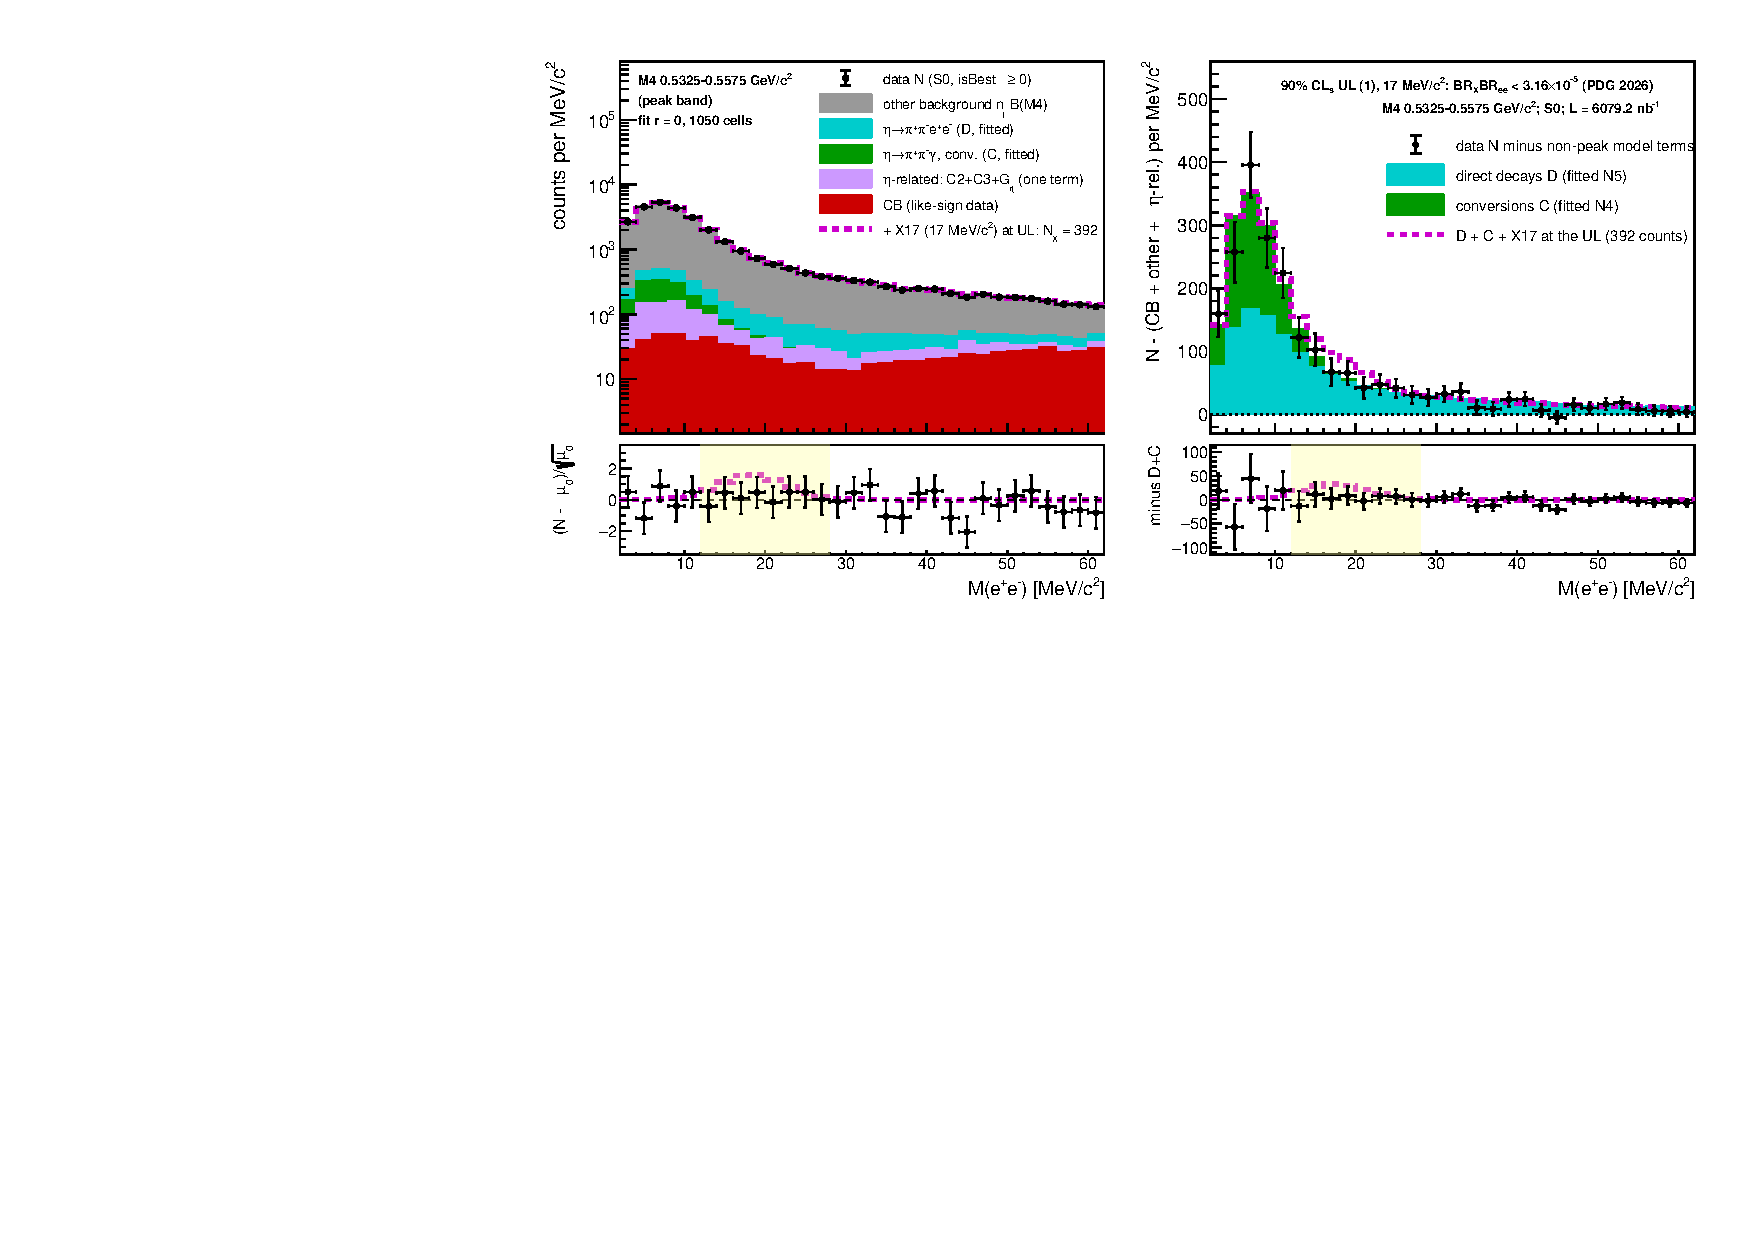
\includegraphics[width=\textwidth]{figs_all/fix_X1_pdg26_cnt.pdf}
\caption{\textbf{What it shows: in the $\eta$ peak band the frozen model without X17 describes the data, also in the \Mee range that was hidden until the freeze; the X17 line at its 90\,\% CL$_s$ limit is drawn for comparison.}
Selection: data at $L=6079.2\,\nbinv$ with the nominal cuts S0 (PT3 trigger; event vertex in the target region, $\vz>-160$\,mm; START-free \betanew identification, pions within 3$\sigma$, leptons within 5$\sigma$ with a RICH ring; energy-loss-corrected momenta of all four tracks; both pions used in the event-vertex fit; all stored combinations of an event, isBest $\ge0$); the $\eta$ peak band \Mfour 0.5325--0.5575\,\GeVcc (ten 2.5\,\MeVcc columns), \Mee 2--62\,\MeVcc; the model fitted with $r=0$ to all cells of the plane \Mfour 0.5225--0.6100\,\GeVcc (35 bins of 2.5\,\MeVcc) $\times$ \Mee 2--62\,\MeVcc (30 bins of 2\,\MeVcc); CB of the like-sign data with the same cuts (10\,\MeVcc cells of \Mfour, shared over the \Mee bins by the like-sign share of each 50\,\MeVcc band), its factor fitted within $1\pm0.5$ for \Mee$<10$\,\MeVcc and $1\pm0.05$ above; SMASH templates with the same cuts (mode A, $w\times$V3, simulated \Mfour$\times0.99615$).
Spec.\ Fig.~X1: \Mee spectrum of the $\eta$ peak band (\Mfour 0.5325--0.5575\,\GeVcc), counts per \MeVcc. Left (log scale): data $N$ (S0, isBest $\ge0$,
black); stacked, the frozen 2D model fitted with $r=0$ to all 1050 cells, in the common colours: CB from like-sign data (red), the $\eta$-related
term (C2+C3 and \Geta, one smoothed term of the frozen model, violet), conversions $\eta\to\pipi\gamma$ $C$ (C4, green), direct $\eta\to\ppee$ $D$
(C5, cyan), other background $n_jB$ (grey); dotted magenta: plus the X17 line
(17\,\MeVcc) at the 90\,\% CL$_s$ limit on the number of X17 counts (392 counts); lower pad $(N-\mu_0)/\sqrt{\mu_0}$ with the X17 at the limit as an expected
pull; yellow band: the \Mee range blinded until the freeze. Right: the same after subtracting the non-peak terms, with the fitted $D$ and $C$ and with
$D+C+$X17 at the limit; lower pad the residual after $D+C$. $L=6079.2\,\nbinv$, raw counts (no 64/63). x17d figure (as corrected by vx)
recoloured (\code{fix_x17X1.C}); the label of the limit with PDG 2026 (\code{x17p26_X1.C}). No fall-back fired on the data.}
\label{fig:X1}
\end{figure}

\begin{figure}[!htbp]
\centering
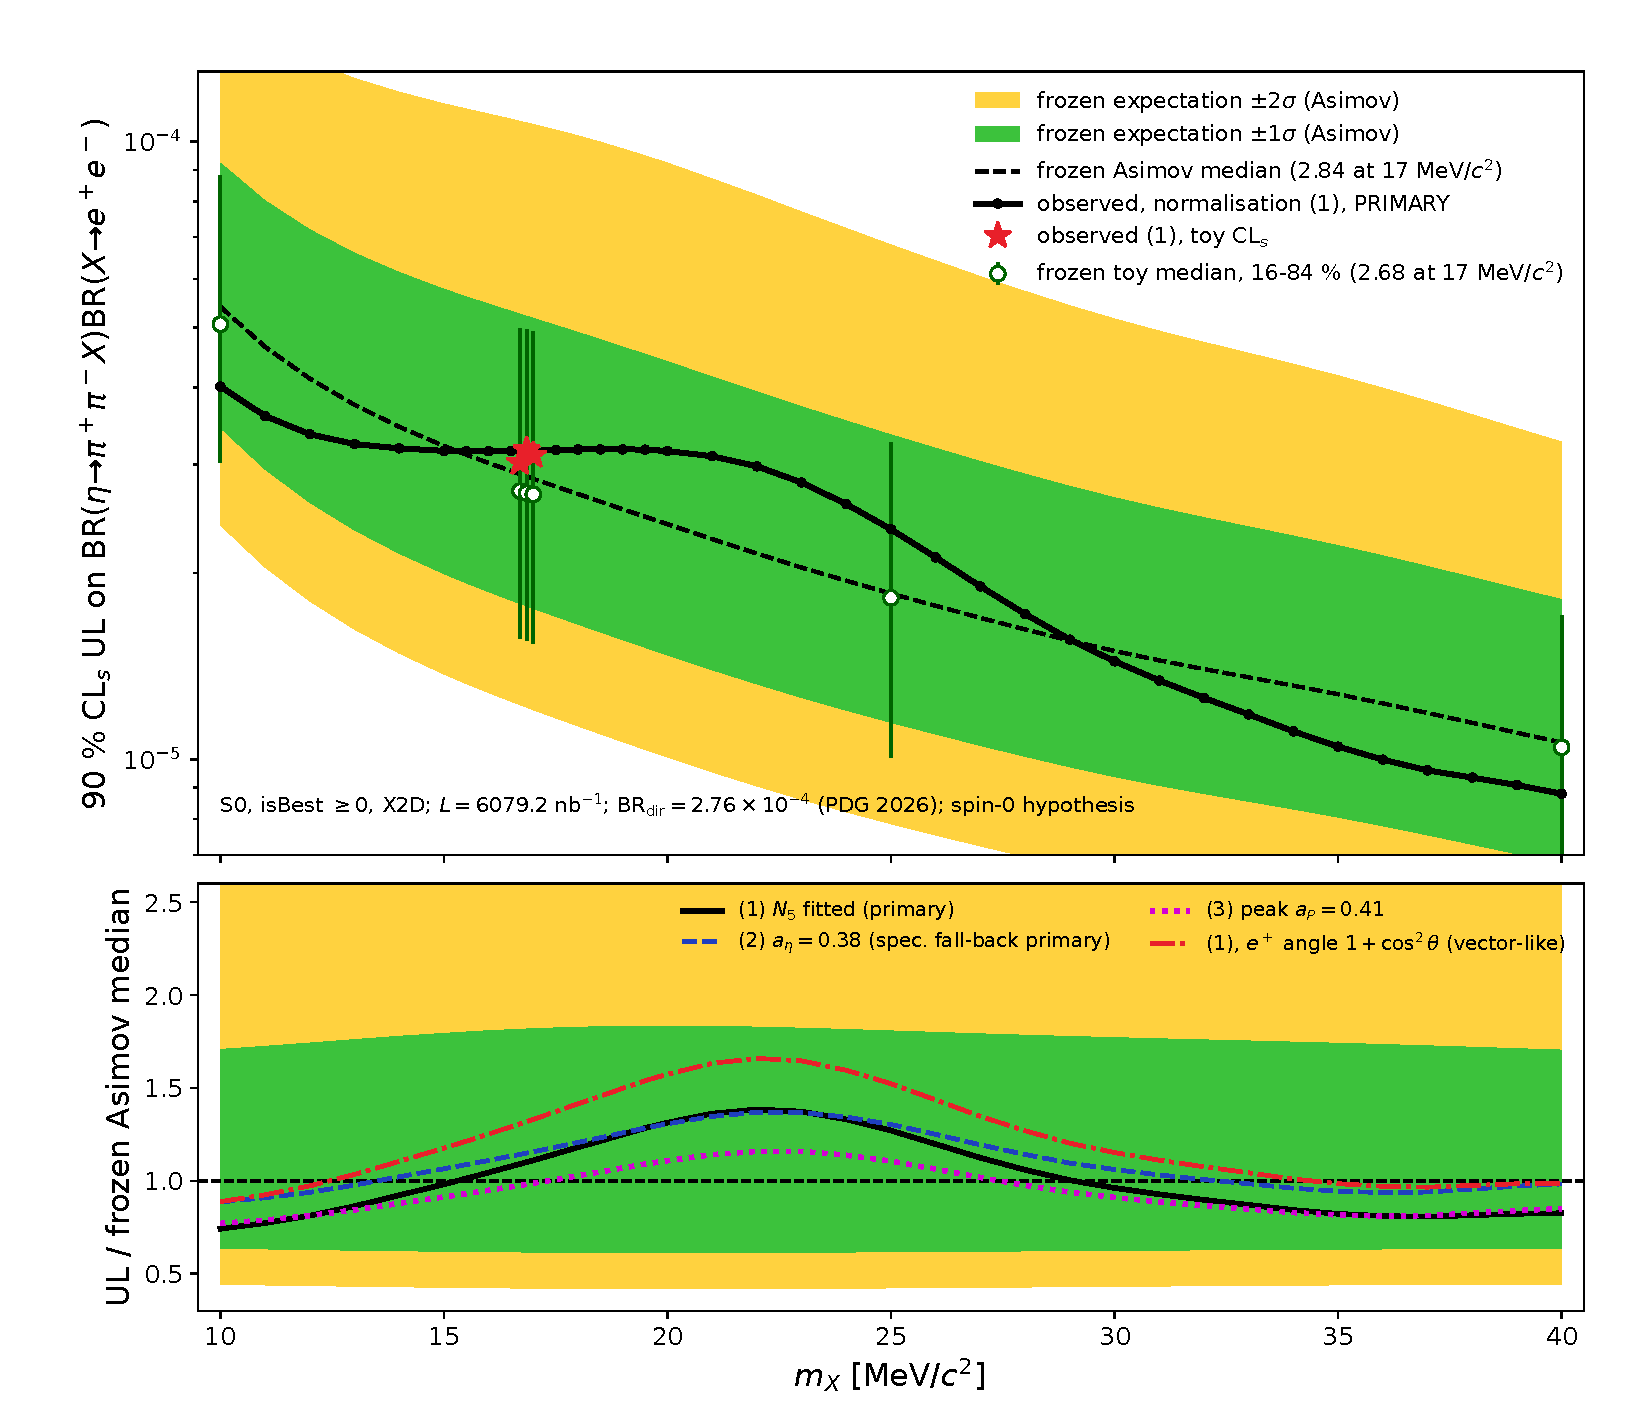
\includegraphics[width=0.80\textwidth]{figs_all/fix_X2_pdg26.pdf}
\caption{\textbf{What it shows: no X17 signal: the observed limit lies inside the frozen $\pm1\sigma$ band of the expected limit at all 38 masses from 10 to 40\,\MeVcc.}
Selection: data at $L=6079.2\,\nbinv$ with the nominal cuts S0 (PT3 trigger; event vertex in the target region, $\vz>-160$\,mm; START-free \betanew identification, pions within 3$\sigma$, leptons within 5$\sigma$ with a RICH ring; energy-loss-corrected momenta of all four tracks; both pions used in the event-vertex fit; all stored combinations of an event, isBest $\ge0$); all cells of the plane \Mfour 0.5225--0.6100\,\GeVcc (35 bins of 2.5\,\MeVcc) $\times$ \Mee 2--62\,\MeVcc (30 bins of 2\,\MeVcc); CB of the like-sign data with the same cuts (10\,\MeVcc cells of \Mfour, shared over the \Mee bins by the like-sign share of each 50\,\MeVcc band), its factor fitted within $1\pm0.5$ for \Mee$<10$\,\MeVcc and $1\pm0.05$ above; SMASH templates with the same cuts (mode A, $w\times$V3, simulated \Mfour$\times0.99615$); the expected bands were frozen from the fit to the \Mee side bands 2--12 and 28--62\,\MeVcc before \Mee 12--28\,\MeVcc was opened.
Spec.\ Fig.~X2: 90\,\% CL$_s$ upper limit on \BRX against $m_X$, 10--40\,\MeVcc (38 masses), spin-0 hypothesis, BR$_{\mathrm{dir}}=2.76\times10^{-4}$
(PDG 2026, D25; the frozen procedure used $2.68\times10^{-4}$). Top: observed, normalisation (1), $N_5$ fitted, primary (black line with points); toy CL$_s$ at 16.7,
16.85, 17.0\,\MeVcc (red stars). Expected, FROZEN before unblinding, two medians: the Asimov median (dashed; $2.84\times10^{-5}$ at 17\,\MeVcc) with its
$\pm1\sigma$ (green) and $\pm2\sigma$ (yellow) bands, and the toy median with 16--84\,\% (open circles; $2.68\times10^{-5}$ at 17\,\MeVcc). Bottom: every
observed curve divided by the frozen Asimov median: (1) black; (2) $\aEta=0.38$ (blue dashed; primary by the specification's fall-back); (3) peak
$\aP=0.41$ (magenta dotted); (1) with the vector-like $e^+$ angle $1+\cos^2\theta$ (red dash-dotted); bands as above. S0, isBest $\ge0$, X2D,
$L=6079.2\,\nbinv$; 2D Poisson likelihood with the frozen nuisances. Redrawn with PDG 2026 from \code{x17d_scan_pdg26.txt} and \code{x17c_expected*_pdg26.txt}
(\code{x17p26_X2.py}; earlier \code{fix_figs.py}): narrower range, variants in the ratio pad. No fall-back fired on the data (D30, approved: normalisation (1) primary, (2) quoted next to it).}
\label{fig:X2}
\end{figure}

\begin{figure}[!htbp]
\centering
\begin{subfigure}{0.42\textwidth}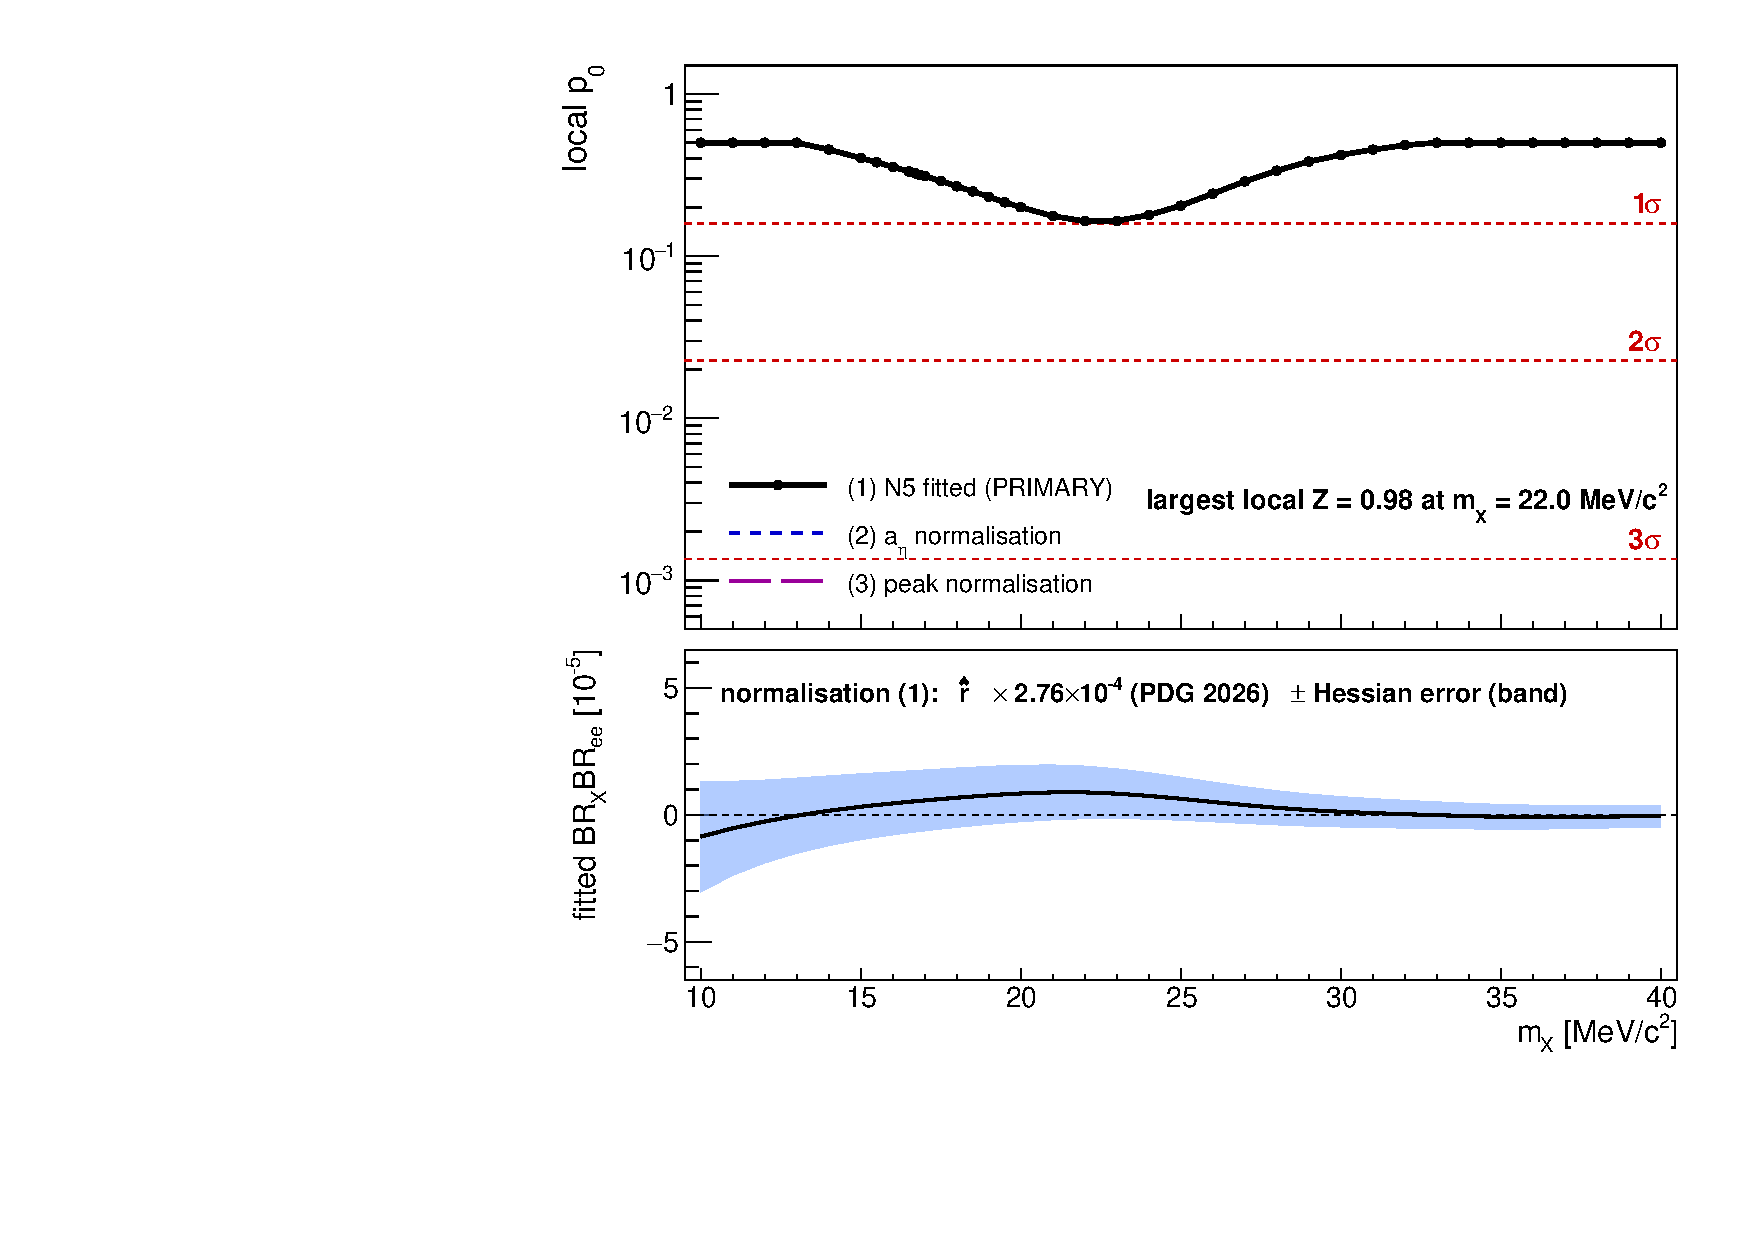
\includegraphics[width=\textwidth]{figs_all/x17d_X3_p0_pdg26.pdf}\caption{}\end{subfigure}
\begin{subfigure}{0.57\textwidth}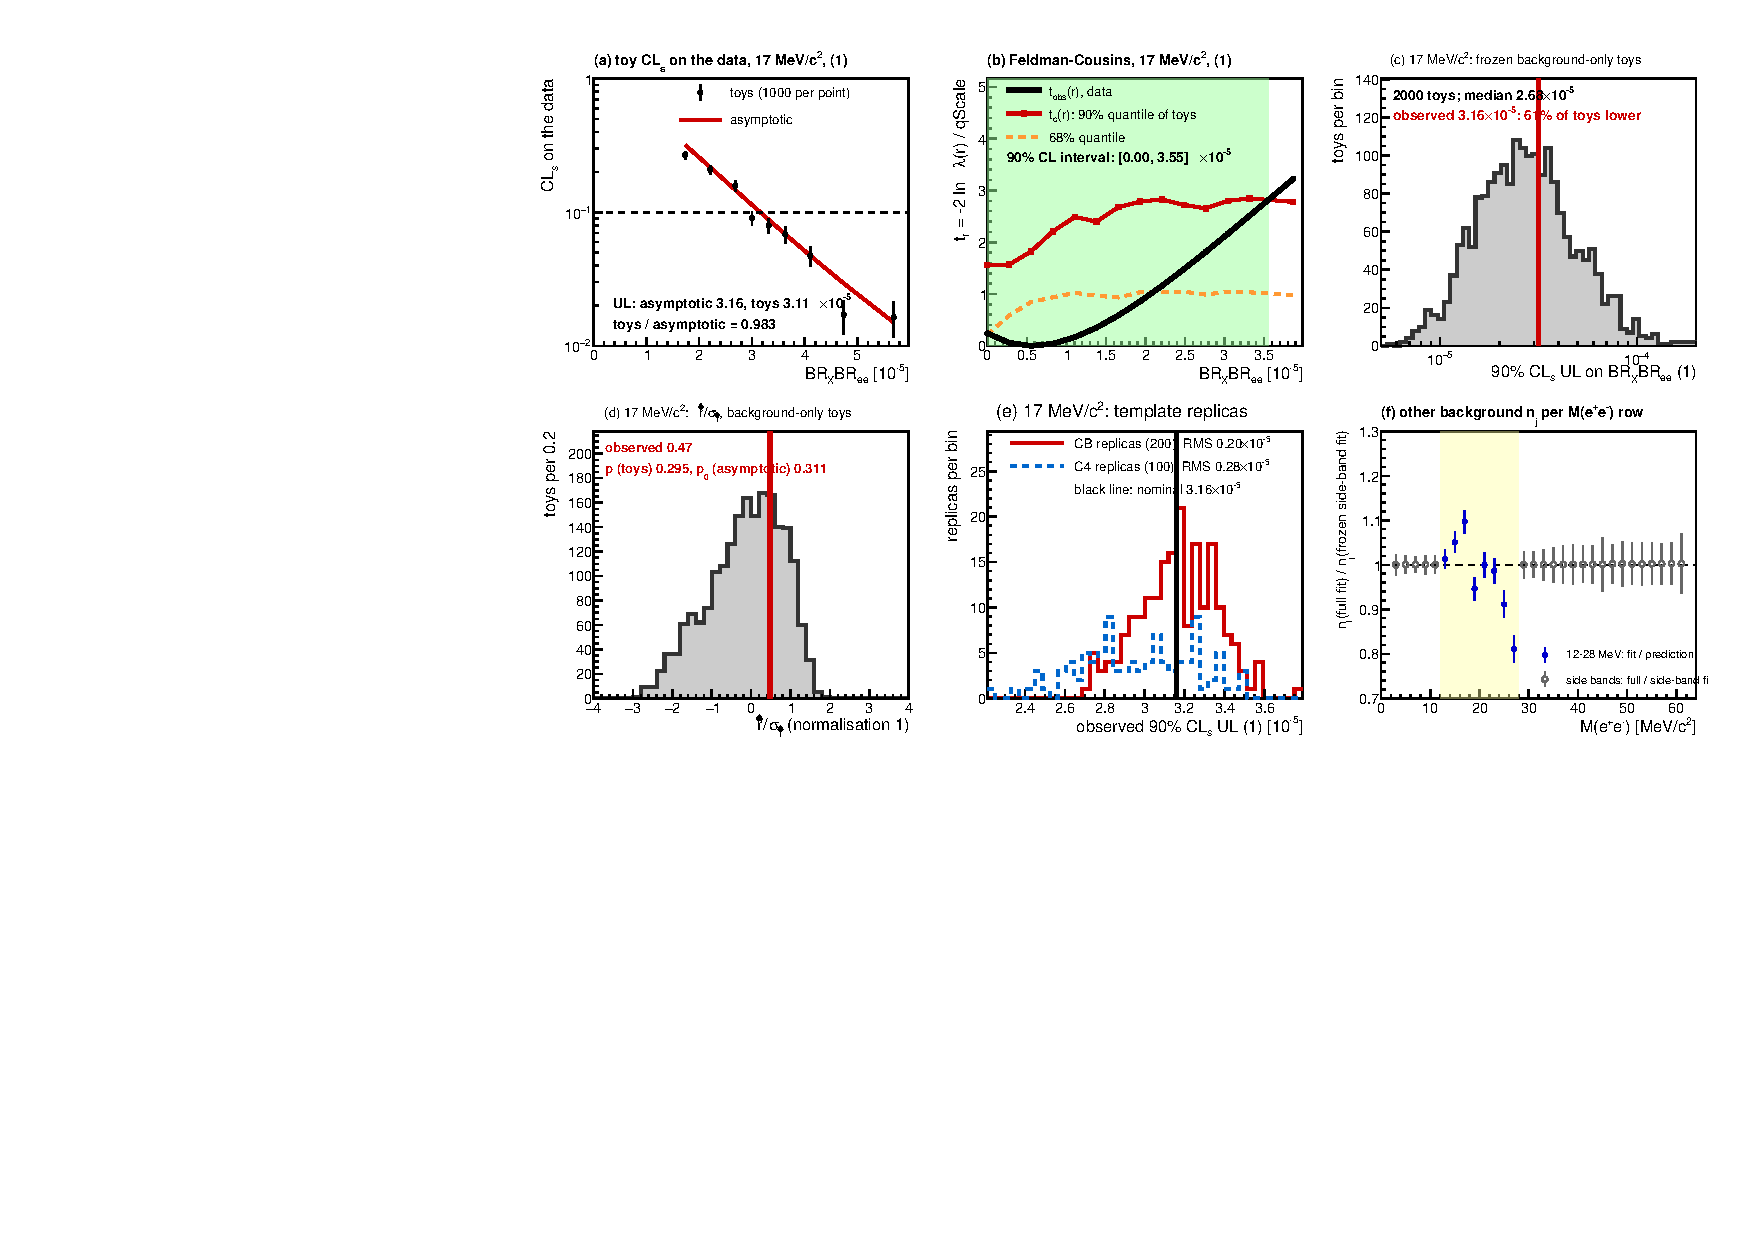
\includegraphics[width=\textwidth]{figs_all/x17d_X4_valid_pdg26.pdf}\caption{}\end{subfigure}
\caption{\textbf{What it shows: no local excess (largest local significance $Z=0.98$ at 22\,\MeVcc); at 17\,\MeVcc the toys confirm the asymptotic limit.}
Selection: data at $L=6079.2\,\nbinv$ with the nominal cuts S0 (PT3 trigger; event vertex in the target region, $\vz>-160$\,mm; START-free \betanew identification, pions within 3$\sigma$, leptons within 5$\sigma$ with a RICH ring; energy-loss-corrected momenta of all four tracks; both pions used in the event-vertex fit; all stored combinations of an event, isBest $\ge0$); all cells of the plane \Mfour 0.5225--0.6100\,\GeVcc (35 bins of 2.5\,\MeVcc) $\times$ \Mee 2--62\,\MeVcc (30 bins of 2\,\MeVcc); CB of the like-sign data with the same cuts (10\,\MeVcc cells of \Mfour, shared over the \Mee bins by the like-sign share of each 50\,\MeVcc band), its factor fitted within $1\pm0.5$ for \Mee$<10$\,\MeVcc and $1\pm0.05$ above; SMASH templates with the same cuts (mode A, $w\times$V3, simulated \Mfour$\times0.99615$); the toys of (b) are drawn from the frozen model in the same plane.
(a) Spec.\ Fig.~X3: local $p_0$ against $m_X$ (asymptotic, $q_0/q$-scale), normalisations (1)--(3) (the curves coincide); bottom: fitted \BRX (1) with its
Hessian error band; largest local $Z=0.98$ at 22\,\MeVcc. (b) Spec.\ Fig.~X4: validation at 17\,\MeVcc: CL$_s$ against BR on the data, toys against the
asymptotic formula (toy/asymptotic UL 0.983); Feldman--Cousins construction (interval $[0,3.55\times10^{-5}]$); the observed limit in the distribution of
the 2000 frozen background-only toy limits (61\,\% lower); observed $\hat r/\sigma$ in the background-only toys (empirical $p$ 0.295, asymptotic 0.311);
the observed limit with 200 CB and 100 C4 template replicas (rms 0.20 and $0.28\times10^{-5}$); background $n_j$ per \Mee row, full fit / frozen side-band
fit (in 12--28\,\MeVcc: measured / frozen prediction). BR axes with PDG 2026 (D25; \code{x17p26_figs.C}). S0, isBest $\ge0$, $L=6079.2\,\nbinv$. No fall-back fired on the data (D30, approved: normalisation (1) primary, (2) quoted next to it).}
\label{fig:X34}
\end{figure}

\textbf{Information only: the model variants on the data} (\code{x17d_variants.txt}; UL / nominal at 17\,\MeVcc, already inside the frozen limit through
the $N_5$ bias (15\,\%) and $s_X$): simulated background exp(pol1) 1.006, exp(pol2) 1.004, exp(pol3) 0.863, \kB 1.005; three classes 0.744, flat pol2
1.166, tilt only 1.154, no \Mee dependence 1.156; CB factorised 0.983, per-row geometric mean 0.992; \kEone free 1.018; V2 1.184, GS 1.006, $r_{\mathrm{res}}=0.89/1.10$
0.976/1.028, $s$ up/down 1.065/0.948. (The systematics table of Part~III, Table~\ref{tab:S1}, has no X17 column; these variants are information only.)

\subsection{Verification of the unblinding}
\label{sec:x17vx}
The verifier vx re-read every frozen file and the X-d code against \code{x17_frozen.txt} (md5 sums unchanged), dumped the data and the sealed file
independently, recomputed the normalisation ($N_5^{\mathrm{ref}}=7458.8$, $s_{\mathrm{X2D}}=3.7446\times10^7$, $R_X=1.3455$, $s_1$, \aP) from the histograms,
and recomputed CL$_s$ by hand from a scan of the profile likelihood ($3.0651\times10^{-5}$ against $3.0646\times10^{-5}$ in the PDG 2020 units of the freeze, a check of the frozen arithmetic; 3.1566 against 3.1561 with PDG 2026). An independent two-step method
(per \Mee row a Poisson fit of the $\eta$-peak yield, then a fit of the 30 yields with $N_5[D+rR_Xf_XX(1+s_X)^\theta]+N_4C$, numpy only) gives:

\begin{table}[H]
\centering
\caption{Independent checks of the observed limit at 16.85\,\MeVcc (verifier vx, \code{vx_indep.txt}, \code{vx_prof_*.txt}), converted to PDG 2026
(D25; the frozen PDG 2020 values of (1) $\times1.030\,k$, of (2) $\times1.0044$). No fall-back fired on the data (D30, approved: normalisation (1) primary, (2) quoted next to it).}
\label{tab:vx}
\small
\begin{tabularx}{\textwidth}{@{}L l >{\raggedright\arraybackslash}p{3.4cm}@{}}
\toprule
check & 90\,\% UL & comment \\
\midrule
frozen, CL$_s$ asymptotic, (1) & $3.160\times10^{-5}$ & toy CL$_s$ $3.17\times10^{-5}$ (PDG 2020: 3.065, 3.07) \\
CL$_s$ recomputed by hand from the profile scan, (1) & $3.157\times10^{-5}$ & arithmetic confirmed (PDG 2020: 3.065) \\
independent two-step method, exp(pol2) background, CL$_s$ & $2.79\times10^{-5}$ & Asimov median 2.76 \\
same, Bayesian with the X17 yield nuisance & $3.20\times10^{-5}$ & 2.94 without it \\
same, background pol1 / pol3 in the exponent, CL$_s$ & $2.94$ / $2.32\times10^{-5}$ & Bayesian 3.41 / 2.80 \\
same, normalisation (2), CL$_s$ / Bayesian & $3.08$ / $3.35\times10^{-5}$ & frozen (2): 3.30 \\
Bayesian, flat prior, on the frozen profile likelihood, (1) / (2) & $4.10$ / $3.91\times10^{-5}$ & $+30$ / $+18$\,\% over CL$_s$ \\
Feldman--Cousins (X-d), 17\,\MeVcc & $[0,\,3.55\times10^{-5}]$ & two-sided \\
\bottomrule
\end{tabularx}
\end{table}

vx found three errors in the spec.\ Table~D1 / spec.\ Fig.~X1 layer, all fixed and none affecting the BR limit: the MC column was the rms of the pooled replica
limits (now CB $\oplus$ C4 in quadrature, $3.47\times10^{-6}$ in (1) with PDG 2026, 3.34 with PDG 2020); the column ``$N_X^{\mathrm{UL}}$'' was a conversion of the BR limit (563 counts), not a limit
on counts (now the direct limit, 392--394); and \sigeta$\times$BR$\times$BR used $1-\fwin$. Caveats (vx): in normalisation (1) the likelihood in $r$ is not
Gaussian (the X17 yield is $rN_5$, and $N_5$ drops from 3659 at $r=0$ to 2696 at the limit), so other constructions give up to $4.1\times10^{-5}$; the C4
replica mean is 6\,\% below the nominal limit, so the nominal is probably about 6\,\% optimistic (about $3.35\times10^{-5}$ with an infinitely precise
template), inside the separately quoted 11\,\%; the independent method moves with the background form ($\hat r\times2.76\times10^{-4}=-1.85\pm1.25\times10^{-5}$
with pol3, about 0 with pol1/pol2, $+0.57\times10^{-5}$ for the frozen fit): all consistent with no signal.

\subsection{Comparison with a simple count (ROOT \code{TRolke})}
\label{sec:trolke}
\notebox{\textbf{In plain words:} counting events in one X17 window with \code{TRolke} gives a limit about 8 times weaker (8.3; $2.6\times10^{-4}$), because
the window's background has to be \emph{predicted} with a 19\,\% uncertainty, while the 2D fit \emph{measures} it. The statistical principle of the two
methods is the same; the difference comes from the information used.}

\textbf{What \code{TRolke} does.} ROOT's \code{TRolke} (W.~A.~Rolke, A.~M.~L\'opez, J.~Conrad, NIM A 551 (2005) 493) computes a confidence interval for
the signal in \emph{one} counting window. The background (and, if wanted, the efficiency) enters with its uncertainty as a nuisance parameter; the
likelihood is profiled over it, and the interval contains all signal values with $-2\Delta\ln L\le2.71$ (90\,\%); with the bounding option the
physical boundary $N_X\ge0$ is respected, which makes it close to the Feldman--Cousins construction.

\textbf{Applied here.} The frozen counting window X17c (\Mfour 0.5312--0.5566\,\GeVcc, \Mee 15.5--24.5\,\MeVcc) holds $N=6424$ counts (6466 with the
cell-overlap rule of X-d); the frozen background prediction is $B=6312\pm1196$ counts. With a Gaussian background and a known efficiency
(model of \code{SetGaussBkgKnownEff}) \code{TRolke} gives $N_X<2083$ counts (2125), and with the frozen conversion $\mathrm{BR}=N_X/(a_\eta s_1)$,
$a_\eta=0.3823$ (0.3806 with the PDG 2026 BR$(\eta\to\pipi\piz)$), $s_1=2.0954\times10^7$: $\BRX<2.6\times10^{-4}$ (2.61 with PDG 2026, 2.60 with
PDG 2020; 2.66 with the overlap count), \textbf{about 8 times weaker} (8.3) than the 2D CL$_s$ limit. BR$_{\mathrm{dir}}$ does not enter this count. Bounded and
unbounded intervals agree, because the count lies above the prediction. Macro \code{plots/all_report/trolke_x17.C}, output
\code{tables_all/trolke_x17.txt} (PDG 2026: \code{trolke_x17_pdg26.txt}).

\textbf{What is similar.} Both are frequentist profile-likelihood methods: the X17 test statistic $\tilde q_r$ of \S\ref{sec:x17model} is also a
ratio of profiled likelihoods with the systematic uncertainties as nuisance parameters. Applied to the full 2D likelihood, the closest equivalent of
\code{TRolke}, the Feldman--Cousins interval with profile-likelihood ordering, gives $[0,\,3.55\times10^{-5}]$ (\S\ref{sec:x17d}), close to the
CL$_s$ limit.

\textbf{Why the count is weaker.} (1) \emph{Information}: the window must \emph{predict} its background, and the prediction carries 19\,\%
(1196 counts, 15 times the statistical error $\sqrt N\approx80$); the 2D fit leaves the background free in every \Mee row and \emph{measures} it from
the \Mfour side bands of that row, and it separates the narrow X17 line (r.m.s.\ about 4.5\,\MeVcc) from the smooth \Mee spectrum of the direct
decays fitted in all 30 rows. (2) \emph{Construction}: \code{TRolke} gives a two-sided (unified-type) interval; CL$_s$ is one-sided and protected
against downward fluctuations. (3) \emph{Coverage}: \code{TRolke} relies on the asymptotic $\chi^2$ threshold, the 2D limit was checked with
pseudo-experiments (\S\ref{sec:x17val}). Point (1) accounts for the factor 8.3.

\subsection{Other searches in this channel}
\label{sec:x17other}
Two earlier searches for a light boson in $\eta\to\pipi\ee$ exist; Table~\ref{tab:x17cmp} (\S\ref{sec:res-x17}) compares them with this
report. \textbf{BESIII} (M.~Ablikim et al., Phys.\ Rev.\ D 111 (2025) 072008, arXiv:2501.10130) used about $1.1\times10^7$ $\eta$ from
$J/\psi\to\gamma\eta$, measured BR$(\eta\to\ppee)=(3.07\pm0.12\pm0.19)\times10^{-4}$ and searched for a narrow axion-like particle $a$ in
$\eta\to\pipi a$, $a\to\ee$ at 5--200\,\MeVcc in 5\,\MeVcc steps. Its 90\,\% CL upper limits (Bayesian) on
$R=\mathrm{BR}(\eta\to\pipi a)\,\mathrm{BR}(a\to\ee)/\mathrm{BR}(\eta\to\ppee)$ are $(3.0$--$53.0)\times10^{-3}$ over the range and about
0.048--0.053 at the two mass points nearest to 17\,\MeVcc (read off their Fig.~7, approximate; no table is published), i.e.\
$0.048$--$0.053\times3.07\times10^{-4}=(1.5$--$1.6)\times10^{-5}$ in absolute terms. \textbf{A preliminary HADES analysis} of the same beam time
(M.~Zieli\'nski, talk ``Search for the Axion-Like-Particles in the $\eta$ meson decay with the HADES Detector'', APS GHP 2025 at the Global
Physics Summit, Anaheim, 15 March 2025) quotes BR $<2.58\times10^{-5}$ (90\,\% CL, an event count with the Rolke method).

The limit of this report near 17\,\MeVcc, $r_{\mathrm{UL}}=0.114$ or $3.16\times10^{-5}$ (CL$_s$, PDG 2026), is therefore about two times weaker than the
BESIII limit (in the edition-free ratio: $r<0.114$ against $R<0.048$--0.053) and numerically similar to the HADES preliminary value. The constructions differ: CL$_s$ here against a Bayesian limit at BESIII (a flat-prior
Bayesian limit on the frozen likelihood of this report is $4.10\times10^{-5}$, Table~\ref{tab:vx}); 38 masses 0.5--1\,\MeVcc apart in 10--40\,\MeVcc
here (\code{tables_all/x17d_scan.txt}) against 5\,\MeVcc steps; $\eta$ produced in p+p at 4.5\,GeV against $J/\psi$ decays; both a spin-0 and a
vector-like X17 here; and a procedure frozen before the unblinding.

The agreement with the HADES preliminary value is \emph{not} a cross-check. That value is an event count with the Rolke method on the same beam
time; the one-window count of this report with the same method (\S\ref{sec:trolke}) gives $\BRX<2.6\times10^{-4}$, about 10 times weaker
($2.6\times10^{-4}/2.58\times10^{-5}\approx10$), because its window must predict the background with a 19\,\% uncertainty. The window, the
background estimate and the normalisation of the preliminary count are not documented in this report, so the reason why that count is so much
stronger than the count here cannot be given.

%======================================================================
\section{Conclusions in detail and open points}
\label{sec:concl}
%======================================================================
\inshort{the results of Section~\ref{sec:results} with all their numbers, variants and caveats; the interpretation D32 proposed by the lead analysis, with its evidence and the separate test ruled by the analyst on 15 November 2026; the full list of open points.}
\textbf{What the data say, described by SMASH.}
\begin{enumerate}\setlength{\itemsep}{0pt}
\item Before any renormalisation SMASH does not describe the shape of the data (data/simulation 0.86 in the bump window, 1.27 above the
      peak, 0.74 at 0.9--1.1\,\GeVcc; $\chi^2$/ndf 12 with one free scale). About 13--15\,\% of $N-\mathrm{CB}$ in 0.40--0.70 is target material
      that SMASH does not simulate; the data hold about 0.3 of the SMASH K$^0_S$ (the event-vertex cut keeps only 0.72--0.85 of it in the data,
      which explains at most a factor 1.4; the rest is not explained) and more \ee pairs above the \piz mass than SMASH. The event-vertex cut
      does not bias these ratios at the 1\,\% level: target events keep their vertex (0.15\,\% of the combinations whose pions cross inside the cell lack
      one; resolution estimate at most 0.8\,\%), and the $\eta$ keeps $0.994\pm0.021$ in the data and 0.9997 in SMASH.
\item The $\eta$ peak is measured: $\Ypeak=5088\pm432\pm584\pm245$ counts in S0, $\sigma_{\mathrm{vis}}=0.837$ visible counts per \nbinv, about 0.40--0.42 of the SMASH
      expectation. The other $\eta$-scale estimates are \emph{consistent cross-checks with a shared normalisation} (the same S0 counts, $L$, the
      simulated efficiencies, whose event-vertex part is now checked against the data, the SMASH kinematics): F-main 0.38, \Pmain 0.40 (0.36 at the
      data-favoured resolution), ECAL tag 0.45 (simulated acceptance verified, photon-energy scale not; verification only); the bump edge, now a
      measurement of its own, gives 0.39--0.43 (item 4). Inside the peak the mix differs from SMASH: the direct decays give 0.50, the conversions 0.24.
\item \sigeta $=0.429\pm0.036\pm0.157\pm0.025^{+0.041}_{-0.043}$\,mb, with the production-model item $^{+0.08}_{-0.03}$\,mb separate (D29,
      ruled), i.e.\ $0.43\pm0.17\,(\mathrm{measurement})\,^{+0.08}_{-0.03}\,(\mathrm{model})$\,mb (PRELIMINARY, D28 ruled: the make-up of the peak is
      open; the normalisation includes the $\pm5$\,\% period
      normalisation of Part~II), $0.40\pm0.16$ of SMASH, with the composition of the peak (from the data) and its low-mass tail (D40) in the
      systematic error. The one-sided
      items (live time, sorter, \code{cor_ok}) would raise it to 0.48\,mb and the measured event-vertex factor by at most 4\,\% more, but
      known-sign items of about the same size would lower it (8--11\,\%); with the direct-decay route 0.58--0.59\,mb (0.70\,mb with its per-class
      side-band value). It is below the published HADES
      inclusive values at 3.5\,GeV (1.14 / 0.93\,mb). The event-vertex cut is not the cause (item 7); no significance is quoted because the
      composition of the peak is not resolved; it is taken from the data provisionally (D31, ruled) until the separate test of D32.
\item \textbf{The bump is measured through its kinematic edge, in the distance to it} (\S\ref{sec:edgeu}): in $u=\Mfour-E(\Mpipi,\Mee)$ all
      edges fall on $u=0$ and one fit finds a step of 21$\sigma$; $f_\eta(u\text{-edge})=0.426\pm0.020\pm0.034\pm0.030$ of SMASH with the C2 decay
      angle corrected by per-count QED weights (D35, D38; 0.390 uncorrected); visible yield in window B $21\,468\pm1003\pm1708\pm1347$ counts;
      \sigeta from the bump alone $0.444\pm0.021\pm0.035\pm0.031\,^{+0.043}_{-0.044}$\,mb (0.407\,mb uncorrected; 0.573\,mb with the conversions
      $\times0.48$); $\mathrm{DR}_u=0.97\pm0.09\pm0.35\pm0.09$ ($\pm0.37$, with the composition term of the peak): a weak test. Systematic error
      8.0\,\% (resolution ratio 4.5\,\%, the step of a smooth background 4.0\,\%, the low-mass tail of the peak 3.4\,\%, CB 2.6\,\%; the phase-space
      Dalitz plots, excluded by KLOE-2 and WP7, would make it 10.6\,\%); the estimator closes within $\pm2$\,\% on pseudo-data and the quadratic term
      that moves B4 by $+150$\,\% moves it by $-2.2$\,\%; MC 7.0\,\% against stat 4.7\,\%; periods ($p=0.024$) and folds ($z=-2.1$) marginal.
      It is the bump measurement (D37, approved). \textbf{The per-slice edge} (\S\ref{sec:bedge}), the cross-check, agrees:
      $0.423\pm0.023\pm0.038\pm0.048$ (0.392 in the frozen convention), 21\,445 counts, \sigeta $0.442$\,mb (0.594\,mb with the conversions
      $\times0.48$), $\mathrm{DR}_{\mathrm{edge}}=0.97\pm0.10\pm0.17\pm0.12$ (24\,\%, without the composition term); determined to 15--20\,\%,
      simulation-limited (MC 0.042--0.048), systematic 8.9--9.0\,\% (11.3\,\% with the Dalitz-plot variants). Like for like the $u$-edge is somewhat
      more precise (11.6 against about 12.4\,\%) but not less model dependent. Both edges use per-count QED weights for the C2 decay angle (D38,
      approved; 0.861 / 0.860 instead of 0.881; $+1.4$ / $+1.2$\,\%). The step of the $e^-e^-$ like-sign counts at $u=0$ ($73.5\pm15.7$,
      4.7$\sigma$) is explained: lepton pairs from the two \piz photons, with the same edge, at \Mee$\ge90$\,\MeVcc, seen mostly as $e^-e^-$
      because of the $e^+$/$e^-$ acceptance and of Compton/knock-on electrons, which are negative only ($e^+e^+$: $7.3\pm4.3$ there); the CB
      removes them as designed ($N-\mathrm{CB}=16.8\pm13.9$ against the expected bump signal 16.9; artefact 2.6$\sigma$ away), it is not a
      charge flip ($<1.2$\,\%), and no number changes (D39, approved; verified). The low-mass tail of the
      SMASH peak term (the leptons' radiation in the material) reaches the edge: $f$ moves by $+6.8$\,\% (per slice $+7.3$\,\%) per unit of its
      size, which the data cannot fix ($t=0.3\pm1.0$); a term of $\pm3.4$ / $\pm3.6$\,\% is counted (D40, approved: total 11.6\,\% instead of
      11.1\,\%). Only the background-subtracted bump area (B4, the main bump estimator by fall-back) and the double ratio derived from it remain
      \textbf{not determined}: the background in the bump window must be extrapolated 40--120\,\MeVcc from above the peak, and a quadratic term
      or a different control region moves B4 by 40--150\,\%.
\item BR$(\eta\to\ppee)$ from the template fits ($\BRG=2.67\times10^{-4}$ with PDG 2026) is consistent with PDG ($2.76\pm0.16$), but the fits failed
      the closure test (attenuation by the noisy signal templates) and the total uncertainty is 90--130\,\%: it is not a measurement.
\item X17: $r<0.114$; $\BRX<3.16\times10^{-5}$ (90\,\% CL$_s$, spin-0, normalisation (1), PDG 2026 BR$_{\mathrm{dir}}$,
      D25)\footnote{With the PDG 2020 value $2.68\times10^{-4}$ fixed in the frozen procedure before the unblinding: $3.06\times10^{-5}$.} at
      16.7--17.0\,\MeVcc; $3.79\times10^{-5}$ for a vector-like X17; 3.16--3.29 between normalisations (1) and
      (2) ((1) is kept against the specification's fall-back, which would make (2), $3.29\times10^{-5}$, primary; D30, approved: (1) primary, (2) quoted next to it);
      about 3.35 with the template-statistics offset. In line
      with the frozen expectation; no signal on 10--40\,\MeVcc. The search is blind in the code, not in the information. The BR limit is free of
      the vertex efficiency; $\sigma\times$BR$\times$BR $<15.6$\,nb (\sigeta uncertainty folded in) contains it through \sigeta (15.7\,nb
      with $C_{\mathrm{vtx}}$ applied).
\item \textbf{Event-vertex efficiency} (measured after the review, \S\ref{sec:vertexeff}): the mandatory cut $\vz>-500$\,mm keeps
      $0.994\pm0.021$ of the $\eta$ in the data ($S$ with a smooth like-sign CB, the ECAL-tagged $T$ and the edge step $E$ combined; $0.990\pm0.022$
      with the CB convention, D33) and 0.9997 in the simulation. The 32\,\% of the combinations without a vertex are off-axis, mostly non-hydrogen events
      (pp-elastic content 0.028 of the cell's, CB$/N$ 0.58) without $\eta$, probably from material in front of the cell (a hypothesis). $C_{\mathrm{vtx}}=1.006\pm0.021$ is not applied and is quoted as a one-sided $+2$\,\% ($+4$\,\% at
      95\,\% CL). The cut is validated, and it is not the cause of the low \sigeta (0.93\,mb would need 0.46).
\item \textbf{A flexible SMASH description} (\S\ref{sec:flex}; a documented description, not a measurement, D36): with a free scale per channel
      the $\eta$ signal classes C2, C4, C5 share one scale, $0.46\pm0.06$ ($p=0.21$; $0.57\pm0.07$ after the template-noise correction); the direct
      decays give $0.63\pm0.12\pm{\approx}0.1$ (0.44--0.94 over the variants), and C5/C2 agrees with the PDG ratio within 1--2$\sigma$; the
      non-$\eta$ background in 0.565--0.70\,\GeVcc is 10--30\,\% above SMASH, its split between $G_D$, $G_C$ and \Geta not determined (80--90\,\%
      correlated). The scales depend on the fit method beyond their errors, the template noise dominates (MC 1--8 $\times$ stat), they cannot be
      carried above 0.70\,\GeVcc, and the model is incomplete (hybrid GLS 604/342, $p<0.001$; the fitted model 2\,\% above the data).
\item \textbf{After the typical cuts of earlier analyses} (\S\ref{sec:e1}, requested comparison, not used for any result): the data exceed SMASH
      as it is by 16--45\,\% at 0.56--0.70\,\GeVcc after every cut (1.23--1.45 on ``pre'', 1.16--1.34 on S0); with $\eta\times0.40$ and the non-$\eta$
      background $\times$1.25--1.52 the S0-based selections are described about as well as S0 ($\delta$ 0.04--0.08, S0\,+\,\cs{X2old} 0.11; S0 0.050); a free $\eta$ scale gives 0.39--0.56.
      The cuts do not enrich the $\eta$; OA$<6^\circ$ keeps 58\,\% of a simulated X17 in its window, but also 57\,\% of the direct decays and 50\,\% of
      the data; S0 alone has the best X17 counting proxy (typical cuts 1.02--1.12, OA$<6^\circ$ 1.20--1.29 relative to S0).
\item \textbf{Full reconstruction of the bump with the ECAL photon} (\S\ref{sec:ecalacc}; feasibility, verification only): one third of the lost
      photons hit an active ECAL module (ECAL sector 0 off; 10.9--45.6$^\circ$ from the target centre; status identical in data and simulation);
      9.8\,\% of the bump combinations are fully reconstructed in the simulation (14.1\,\% at a data-like energy scale), about 12\,\% in the data, as a clean
      peak (stat 3.2\,\% against 5.4\,\% for the edge). Data/expected $1.16\pm0.21$ with the simulated photon-energy scale, $0.84\pm0.15$ with a
      data-like one (errors overestimated), one factor at every \Mpipi. Needed: the photon energy scale and resolution (data $+17$\,\%, simulation
      $-7$ to $-9$\,\%), the module efficiency (65\,\% in the simulation, not explained), a START-free photon cut (events without START lose 20--30\,\%
      of their tags, 1.4--2.3\,\% of $T$), and at least 10 times more simulated $\eta\to\pipi\piz$; it connects with the separate ECAL analysis of
      D32.
\end{enumerate}

\notebox{\textbf{Interpretation proposed by the lead analysis; ruled by the analyst on 15 November 2026 to be tested in a separate analysis
(D32; it changes no number of this report).} With the vertex cut excluded as a cause,
part of the $\eta$-scale numbers of this report would fit together if the \emph{data lose close \ee pairs} (small opening angle, small \Mee)
\emph{more than the simulation does}. The evidence is suggestive, not conclusive:
\begin{itemize}\setlength{\itemsep}{0pt}
\item The direct decays $\eta\to\ppee$ (C5, pairs spread to large \Mee) give the highest scale: direct-decay route $a=0.497\pm0.059$ (stat; side
      bands per \Mee class $0.592\pm0.139$, X17 2D fit $0.476\pm0.065$). Its systematic error is not small: 82\,\% of its weight is $N_5$ of the X17
      template fit, whose half spread over the background and CB variants is 10.9\,\%, which moves by $+22$\,\% with three background classes, and
      which came out $+55$\,\% on the simulation-study toys of the specification (x17ab). F-main gives a similar value through its direct-decay
      factor, $\rhod\times\aEta=0.488$ (PDG 2026; 0.50 with PDG 2020), but F-main failed the closure test and is a cross-check only.
\item The conversion route (C4, $\eta\to\pipi\gamma$ with a converted photon, \Mee of a few \MeVcc), a close-pair class, is lower: $0.237\pm0.049$.
\item The bump (\piz Dalitz pairs and conversions, C2+C3) does not decide: B4 ($a_B(\mathrm{all})=0.299$, $a_B(E2)=0.312$) is NOT DETERMINED
      (systematic 157--165\,\%); the bump edge, now measured, gives 0.426 in $u$ (\S\ref{sec:edgeu}; 0.423 per slice, \S\ref{sec:bedge}; in the
      first version 1.4$\sigma$ below the direct route) with the simulated conversion rate and 0.549 (0.569) with the conversions $\times0.48$, and
      its own \Mee split gives $\kappa=0.83\pm0.20\pm0.34$ in $u$ ($0.47\pm0.24\pm0.46$ per slice), consistent with 1 and with 0.48, too imprecise
      to choose; and $f_\eta(\mathrm{tag})=0.454\pm0.043$, which uses the close \piz Dalitz pairs ($\Mee<0.10$\,\GeVcc) of the same C2 decay, sits
      with the direct route (0.6$\sigma$), but the expected tag moves by a factor 1.46 with the photon-energy scale (data/expected 1.16 to
      0.79--0.84, \S\ref{sec:ecalacc}), so today the tag tests the $\eta$ scale only to about $\pm20$\,\% and favours no route (verification only).
\item The data peak is more E2-like than SMASH: its share at \Mee$\ge10$\,\MeVcc is $0.546\pm0.053$ against 0.425 in SMASH (C4/C5 shapes of the
      side-band fit; 0.423 in WP8's sums), 2.3$\sigma$.
\item A known simulation defect points the same way: HGeant decays the $\gamma^*$ of C2 isotropically, so the simulated efficiency of the C2
      bump counts is about 16\,\% too high (12--14\,\% in the toys and the closure; \S\ref{sec:eff}); its per-count correction (D38) raises the
      bump-edge scales by 8--9\,\% and is applied.
\end{itemize}
If the close-pair classes (C4, C2, C3) have a lower efficiency in the data than in the simulation (for example through track merging, shared
RICH rings or the lepton identification of close tracks), while the direct decays at larger \Mee are described, then the direct decays would give
the most reliable $\eta$-production scale, and \sigeta $\approx0.52\pm0.06\,(\mathrm{stat})$\,mb by that route (0.58--0.59\,mb with the one-sided
items), against the adopted 0.429\,mb, which mixes both routes. The headline numbers stay as they are: the composition systematic ($\pm32$\,\%)
already spans the two readings. \textbf{The test, as ruled by the analyst on 15 November 2026 (D32)}: a \emph{separate} analysis, not part
of these reports, measures the reconstruction efficiency of \ee pairs with an opening angle of 0--6$^\circ$ in data and simulation, from \piz,
$\eta$ and $\omega$ Dalitz decays (the \ee hypothesis plus the ECAL photon). It waits for the trigger-bias correction and the new ECAL calibration
(both in progress); its results will be brought into these reports. \textbf{What follows (D31, ruled, option (a))}: until then the make-up of the
peak is taken from the data (0.43\,mb, composition term $\pm32$\,\%, systematic 35.5\,\%, 36.6\,\% with the peak tail of D40), provisionally. If
the test confirms that the data lose close pairs, the direct-decay route (0.52\,mb) becomes the natural headline with a much smaller composition
term, and the bump gives 0.57\,mb with the conversions $\times0.48$ (0.573\,mb in $u$, 0.594\,mb per slice); if it does not, the routes must differ through the simulated material
(conversions) or the direct-decay rate, and 0.43\,mb with its $\pm32$\,\% stays.}

\textbf{Open points} (for the analyst; the first three limit the absolute results):
\begin{enumerate}\setlength{\itemsep}{0pt}
\item \textbf{Close-pair efficiency} of data against simulation: the separate analysis of D32 (pairs with OA 0--6$^\circ$ from \piz, $\eta$
      and $\omega$ Dalitz decays with the ECAL photon; after the trigger-bias correction and the new ECAL calibration): it can confirm the
      direct-decay route (\sigeta 0.52\,mb; the conversion route gives 0.25\,mb); if it shows no loss, the question stays open. It is now the largest open item of every absolute statement.
      (The event-vertex efficiency, open point 1 of the first version, is measured, \S\ref{sec:vertexeff}. Still unchecked is which vertex
      condition the elastic luminosity used: about 1\,\% if it used none; not estimated if it required the DST vertex; to be checked in the
      luminosity analysis.)
\item \textbf{Simulation statistics}: every template fit and B4 are simulation-limited (MC/stat 2--4), and so are the bump edges (per slice
      MC/stat 2; in $u$, with the simulated step from the bump classes alone, MC 7.0\,\% against stat 4.7\,\%; the same rule would give about
      6.6\,\% per slice), the ECAL tag (MC of $T_{\mathrm{sim}}$ 8.9\,\%) and the flexible description (MC/stat 1--8); a larger standard-set
      production is requested (fall-back of the specification), and a forced $\eta\to\pipi\piz$ production with the full ECAL simulation, at
      least 10 times the present 2836 simulated C2+C3 entries. Smoothed or factorised signal templates would remove
      the attenuation of the template fits.
\item \textbf{The bump background below the peak}: neither a linear nor a quadratic extrapolation closes in CR-L, CR-K and 0.400--0.455
      (\S\ref{sec:closure}); a control region with a known bump-free shape is still missing for the bump \emph{area} (B4). The bump yield itself
      now comes from the edge, which relies on the absence of background structures as narrow as the edge (none seen).
\item \textbf{QED $\gamma^*$ decay angle} of class C2 (HGeant isotropic): the bump edges use per-count QED weights, the circle average of the
      full simulation (0.860--0.861 at the edges; D38, approved, \S\ref{sec:c2recon}), to be applied until a future simulation corrects the angle
      in GEANT itself (not expected); an exact correction would need the true photon or \piz momentum per C2 entry in the compact file
      (\S\ref{sec:eff}).
\item \textbf{Class E1} (\Mee$<10$\,\MeVcc) is not described (\kEone$=7.6$--13.2); every all-\Mee yield is extrapolated from E2 with the simulated
      \Mee shape (supported by the tagged-$\eta$ E2 share within 4--8\,\%). Data and SMASH side by side in $u$ (\S\ref{sec:edgeu-sim},
      Fig.~\ref{fig:res-udatasim}) show the same: with the measured scales SMASH reproduces the position and the width of the step and the peak
      region (the step size is fitted, so it is not a test) and describes the data for \Mee$\ge10$\,\MeVcc ($\chi^2=37.0/36$), but the stage-A
      background, fitted for \Mee$\ge10$\,\MeVcc, puts the model 1/0.65 too high below 10\,\MeVcc (1/0.76 for all \Mee; the E1 data want a
      conversion scale of about 1.5--1.7 instead of $\kB=3.06\pm1.45$, 1.6--1.9 standard deviations of the stage-A error); $f_\eta$ is not affected.
\item \textbf{$g$ (\Geta scale)} is not robust (0.47--2.6 over estimators and variants; 1.1--3.9 in the flexible fit, depending on the fit
      weights); the side bands depend on it only through the background ratio $R'$.
\item \textbf{The flexible SMASH description is incomplete} ($p<0.001$; no description above \Mfour$=0.70$\,\GeVcc with scaled components): which
      background SMASH lacks (target material, 13--15\,\% of $N-\mathrm{CB}$, is one candidate) and how the non-$\eta$ excess above the peak splits
      between $G_D$, $G_C$ and \Geta are open (\S\ref{sec:flex}).
\item \textbf{Ghost ruling} (D6) pending; variant (a) lowers the ``before'' ratios by 8.5--14.5\,\% ($J$ by 6.6\,\%).
\item The \textbf{production-model item} of \sigeta ($^{+19}_{-7}$\,\% from the 1D $p_T$/$y$ reweighting) is kept separate from the total by
      the analyst's ruling (D29, 15 November 2026): $^{+0.08}_{-0.03}$\,mb. The \textbf{composition of the peak} is taken from the data
      ($\pm31.8$\,\%, D31, ruled: provisionally, until the test of D32): the direct decays
      (side bands per \Mee class, X17 fit) give 0.50, the conversions 0.24; which SMASH component is wrong (conversion material and close-pair
      efficiency, or the direct-decay rate) is open; it sets \sigeta between 0.25 and 0.52\,mb (the test of D32, item 1, can confirm the
      direct-decay route).
\item The \textbf{\Mee scale and resolution} priors of the X17 fit ($\pm2$\,\%, $\pm10$\,\%) were not checked on the E1 conversion peak (one 2\,\MeVcc bin in
      the factory layouts).
\item \textbf{Blinding}: coarse \Mee information (G3 classes, OA in 1$^\circ$ bins) was not masked in the factory file (v0); no package formed it in
      the peak band. Part~II published the \Mee spectrum of the peak band in 3\,\MeVcc bins before the freeze (\S\ref{sec:blind}): blind in the code,
      not in the information.
\item \textbf{Decisions} (Table~\ref{tab:decisions}). All of D21--D40 were ruled by the analyst on 15 November 2026: D21 (Amendment~1,
      approved), D22 (closure gate, approved), D23 (template covariance in D11 and stage A, approved), D24 (systematics rules MC($\Delta$) and
      R1, approved), D25 (PDG 2026 everywhere, also for the X17 limit), D26 (deficit span 034--045, approved; PT2 check), D27
      ($\eta_{\mathrm{U}}$ in B4, approved), D28 (PRELIMINARY kept, because the make-up of the peak is open), D29 (production model separate), D30
      (X17 normalisation (1) primary, (2) quoted next to it), D31 (composition from the data, provisional), D32 (a separate analysis), D33
      (vertex study, approved), D34 (typical cuts not applied, variants shown), D35 (C2 correction of the bump edge, approved), D36 (flexible
      model, approved), D37 ($u$-edge as the bump measurement), D38 (per-count C2 weights), D39 (the $e^-e^-$ like-sign step: cross-photon
      pairs, CB unchanged) and D40 (the tail of the $\eta$ peak term, option (a)). Still awaiting the analyst: the deviations and fall-backs among
      D1--D20.
\item \textbf{The tail of the $\eta$ peak term} (D40, \S\ref{sec:edgeu-tail}): the leptons' radiation in the material (HGeant) gives the
      simulated peak a low-mass tail that reaches the bump edge; the data cannot measure its size ($t=0.3\pm1.0$); a larger simulated
      $\eta\to\pipi\gamma$ sample, a simulation with final-state radiation and the data peak position against \Mpipi would make it measurable.
      Until then $t=1\pm0.5$ is used (D40, approved: $\pm3.4$\,\% on $f_\eta(u\text{-edge})$, $\pm8.8$\,\% on \sigeta from the peak).
\item \textbf{ECAL full reconstruction}: requirements (1)--(4) of \S\ref{sec:ecalacc-need} (photon energy scale and resolution, module efficiency,
      a START-free photon cut, more simulation); it connects with the separate ECAL analysis of D32.
\end{enumerate}

\appendix
\part*{Reference material}
\addcontentsline{toc}{part}{Reference material}

%======================================================================
\section{Decisions of the analyst (ruled and open)}
\label{sec:decisions}
%======================================================================
The specification of this part was agreed before any data yield was looked at. Its decisions D1--D20 are listed here with their
reasons and with what happened to each of them during the analysis (last column). The decisions that were taken later, by a work
package, a verifier, the lead analyst (Amendment~1, normalisation of the $\eta$ yields with $1-\feta$ instead of $1-\fwin$) or the review,
and that change results, follow as D21--D33 with the deciding package and their effect; D34 came with the comparison after the typical cuts,
D35 and D36 with the bump-edge measurement and the flexible SMASH description, D37--D39 with the $u$-edge, the per-count check of the C2
factor and the like-sign step, and D40 with the tail of the $\eta$ peak term (15 November). Several come from the lead analysis itself: D21
(Amendment~1), D32 (an interpretation), D35--D40.
D21--D40 were all ruled by the analyst on 15 November 2026 (status column, ``Ruled by the analyst on 15 November 2026: \dots''; D22--D24, D30,
D33 and D37--D40 in the evening, D40 with option (a)). Still awaiting the analyst: the deviations and fall-backs among D1--D20 (D5 E1 dropped, D6
ghost ruling, D9 CR-K dropped, D11 template covariance, D12/D15 demoted, D19 blind in the code only, D20 gate configuration; the related later
decisions D23, on D11, and D22, on the gate configuration, are approved, but the analyst has not ruled on these deviations within D1--D20 as such).

{\footnotesize
\setlength{\tabcolsep}{3pt}
\renewcommand{\arraystretch}{1.08}
\begin{longtable}{@{}>{\raggedright\arraybackslash}p{0.6cm} >{\raggedright\arraybackslash}p{5.2cm} >{\raggedright\arraybackslash}p{4.6cm} >{\raggedright\arraybackslash}p{\dimexpr\textwidth-10.4cm-6\tabcolsep\relax}@{}}
\caption{\textbf{Decisions D1--D20} of the specification, their reasons and their status after the analysis, and the decisions D21--D33
taken during the analysis or the review; D34 was added with the comparison after the typical cuts (\S\ref{sec:e1}), D35 and D36 with the bump
edge (\S\ref{sec:bedge}) and the flexible SMASH description (\S\ref{sec:flex}); D37--D40 with the $u$-edge (\S\ref{sec:edgeu}), the per-count C2
factor (\S\ref{sec:c2recon}), the like-sign step (\S\ref{sec:edgeu-ls}) and the tail of the peak term (\S\ref{sec:edgeu-tail}), 15 November. ``Applied'' means as
specified; deviations and fall-backs are named with the section where they are described.}\label{tab:decisions}\\
\toprule
\# & decision & reason & status in this report \\
\midrule
\endfirsthead
\toprule
\# & decision & reason & status in this report \\
\midrule
\endhead
\bottomrule
\endfoot
D1 & Nominal selection S0 = ``pre'' + both pions in the vertex fit, for bump, peak and X17; ``pre'' is a full parallel column. &
CB/$N$ falls from 0.13 to 0.06; S0 is the frozen X17 selection; simulated $F/F_{\mathrm{best}}$ 0.95--0.98; efficiencies cancel in ratios. &
Applied. ``pre'' is refitted in every package (Tables~\ref{tab:B1}, \ref{tab:E1}; family S11). \\
D2 & isBest $\ge0$ nominal; isBest $=1$ gives data-only yield ratios. & Analyst rule; the simulated isBest is unrealistic in the lepton set. &
Applied: isBest $=1$/isBest $\ge0$ $=0.87$--0.92 for the yields, 1.02--1.05 for the ratios (\S\ref{sec:cons}). \\
D3 & No upper cuts on \MMfour, \Mpipi, the $\eta$-rest angle or OA. & Sculpting and band-pass effects measured in data (Part~II). & Applied. \\
D4 & DIRECT ($\dzpi<40$\,mm) is a variant; PEAK ($+\MMfour<2.85$) only after a fake-peak test, simulated \MMfour at 4500\,MeV. &
\MMfour sculpts; the simulation was generated at 4500\,MeV. & DIRECT used in family S11. PEAK histograms exist (\S\ref{sec:factory}) but were not refitted here; Part~II recommends PEAK for the data-only peak. \\
D5 & CB $=2\sqrt{N_{++}N_{--}}$, $k=1$, never from simulation; nuisances $\kEtwo=1\pm0.05$, \kEone free. & Analyst rule; no 4-body $k$ exists; the CB at small OA is a lower limit. &
Applied. \kEone came out at 13.2 (stage A) and 7.6 (stage B): fall-back, E1 dropped (\S\ref{sec:step0}). X17 uses $\kEone=1\pm0.5$ (\S\ref{sec:x17model}). \\
D6 & Simulation std + lep + $\eta$, owned entries (mode A), $w\times$V3 (code 108), T1 + T2, every channel at SMASH $\sigma_{\mathrm{prod}}\times$ PDG BR; ghost variant (a) as a systematic. &
Rules v2; the ghost ruling is pending. & Applied. Variant (a) raises the simulation by 9--17\,\% and lowers the ``before'' ratios by 8.5--14.5\,\% per region ($J$ by 6.6\,\%, \S\ref{sec:before}); family S4. Ghost ruling still pending. \\
D7 & Data unit $(N-\mathrm{CB})\times64/63/L$, $L=6079.2\,\nbinv$; simulation $\sum w/221.05\,\nbinv$; old tables $\times1.0161$. &
Analysed runs; PT3 trigger-bit prescription; old tables used 6080.5 and no 64/63. & Applied; the old table is reproduced to $5\times10^{-4}$ (\S\ref{sec:wp1acc}). \\
D8 & Simulated $M_4'=s\,[m_4^{\mathrm{true}}+r_{\mathrm{res}}(m_4-m_4^{\mathrm{true}})]$, $s=0.99615$, $r_{\mathrm{res}}=1$; \Mpipi$\times0.9952$; \Mee not scaled. &
Peak shift 0.5439 vs 0.5460 significant; width 5.44 vs 6.09\,\MeVcc only $1.1\sigma$. & Applied. A free $s$ is $+1.95\sigma$ (whole fit) and $-2.0\sigma$ (peak region): marginal (\S\ref{sec:mscale}). The measured width favours $r_{\mathrm{res}}=0.89$ ($\sigma_\eta$ $-10.8$\,\%, known sign, \S\ref{sec:p2}). \\
D9 & Control regions: the $\eta$-free part of the \Mfour$\times$\Mpipi plane (CR-U, CR-K); CR-L and displaced windows are tests. &
\Mfour alone has no signal-free region below the bump; CR-K is kinematically bump-free. & \textbf{Fall-back}: CR-K failed A1/A2 and was dropped; CR-U starts at 0.575\,\GeVcc (\S\ref{sec:crchoice}). \\
D10 & Only the non-$\eta$ background is renormalised; every $\eta$ component scales with \aEta; \Geta also gets $g=1\pm0.30$. &
$\eta$ 0.3--0.5, background 1.3--1.4 of SMASH; \Geta is 6.4\,\% of CR-U and 37\,\% of the simulated peak. & Applied. The fit pulls $g$ to $1.72\pm0.40$; over estimators and variants $g$ ranges 0.47--2.6; family S8 widened to this range in the review (\S\ref{sec:syst}). \\
D11 & Background $c_j(1+bx)$; a quadratic term, then per-slice tilts, only if $\Delta\chi^2>4$ in stage A. &
$\chi^2$/ndf 3.8 (scale only) $\to$ 1.3 (tilt). & Applied with a $\chi^2$ that includes the template covariance (deviation, \S\ref{sec:d11}); the data-only choice is a family-S3 variant. \\
D12 & Main extraction: Poisson likelihood of the unsubtracted $N$, 5 \Mpipi slices $\times$ 2 \Mee classes, \Mfour 0.400--0.700. &
The moving edge and the \Mee split break the tilt/bump degeneracy. & Implemented (F-main), but it \textbf{failed} the closure test (\S\ref{sec:val}): cross-check only. \\
D13 & Non-$\eta$ templates smoothed with exp(pol3); signal templates raw with BB-lite; MC error separate. &
One standard-set entry $=27.5$ data counts; $G_{\mathrm{conv}}$ has $N_{\mathrm{eff}}=18$ in the X17 window. & Applied. The raw signal templates bias every template fit by about $-10$\,\% (\S\ref{sec:val}). X17 uses exp(pol2) and smoothed $\eta$-related terms (\S\ref{sec:x17model}). \\
D14 & Side-band estimators reported next to the fit, not combined; \Pmain, the edge step and the ECAL tag only as cross-checks. &
Transparency; the simulated ECAL tag is emulated (later: its acceptance verified, its photon-energy scale not, \S\ref{sec:ecalacc}). & Applied. By fall-back the side bands are now the \emph{main} result (\S\ref{sec:sb}). The edge step was later made a measurement of the bump (\S\ref{sec:bedge}, D35); the ECAL tag stays verification only. \\
D15 & BR$(\eta\to\ppee)$: primary the golden ratio (\Mee$\ge20$\,\MeVcc relative to the bump), then $\rho_d$, then the conversion route. &
The golden ratio is free of $L$, $\sigma_\eta$, PT3, live time and material. & F-gold failed the closure test: \BRG is a cross-check; \BRC withdrawn (\S\ref{sec:ffree}). No BR estimator is validated. \\
D16 & \sigeta is secondary and needs the normalisation items. & $L$ is LH$_2$ only; the PT3 sector-2 deficit is not in $L$. & Done (\S\ref{sec:norm}); Amendment~1: $\Csec(1-\feta)=0.98$. Labelled PRELIMINARY (\S\ref{sec:p2}). \\
D17 & Live time not applied; one-sided $+7.3/-0$\,\% on cross sections. & Unknown whether it applies to PT3 single-interaction events. & Applied (the verifier gives $+7.1$ to $+7.3$\,\%). \\
D18 & X17: 2D Poisson likelihood, background free per \Mee bin (from data); POI $r$ $=$ BR$_X$\,BR$_{ee}$\,/\,BR$_{\mathrm{dir}}$ in the same fit; 90\,\% CL$_s$. &
No simulated background per bin; nothing used twice. & Applied and frozen before unblinding (\S\ref{sec:x17freeze}). \\
D19 & Blinding: window count (5258, CB 112) and \Mee$>20$\,\MeVcc peak share (0.306) already known; the 2\,\MeVcc \Mee shape of the peak band in 13--27\,\MeVcc masked until \code{x17_frozen.txt} exists. &
Honest blinding. & Applied in the code (\S\ref{sec:blind}), \textbf{not in the information}: Part~II (\S7.7 there) showed the side-band-subtracted \Mee spectrum of the peak band in 3\,\MeVcc bins across 13--27\,\MeVcc before the freeze. CB of the window: 112 (geometric mean of the window), $171\pm6$ (spread rule of this report), 102 (Part~II's rule). \\
D20 & No data yield is shown before its estimator passes the closure test. & The earlier blind test was not blind by construction. & Applied: the closure verdicts (\S\ref{sec:val}) were fixed before any yield was quoted; the gate configuration (RF instead of BA) was chosen after the BA results were seen (D22, approved). \\
\midrule
\multicolumn{4}{@{}p{\textwidth}@{}}{\emph{D21--D33: decisions taken during the analysis (decision, deciding package, effect). \textbf{D21--D33 were all ruled
by the analyst on 15 November 2026 (D22--D24, D30 and D33 approved in the evening).}}} \\
D21 & Amendment~1: $\eta$ yields use $1-\feta$ ($\feta=3^{+4}_{-3}$\,\%), never $1-\fwin$. & Lead analyst after WP2 and its verification. & \sigeta $\times0.97$ instead of $\times0.832$ ($+17$\,\%); the nucleon-count expectation 5--12\,\% is only partly covered (\S\ref{sec:norm}). \textbf{Ruled by the analyst on 15 November 2026: approved}; $\eta$ yields $\times(1-\feta)$, $\feta=3^{+4}_{-3}$\,\% (Amendment~1), never $1-\fwin$. \\
D22 & Closure gate: method configurations + RF instead of the specified BA. & WP4 (BA has four times the template noise of the analysis). & Under BA every estimator fails (peak side bands $+14$\,\% in b$-$); with RB the peak side bands are FAIL marginal (\S\ref{sec:val}). \textbf{Ruled by the analyst on 15 November 2026: approved} (as proposed). \\
D23 & D11 and the stage-A $\chi^2$ criterion judged with the template covariance (GLS). & WP3. & M1 kept; data-only chain $\to$ per-slice tilts + quadratic + $\omega$ split (B4 $+153$\,\%). With the hybrid GLS of the review M1$\to$M2 has $\Delta\chi^2=4.2$--4.5 (borderline, \S\ref{sec:d11}). \textbf{Ruled by the analyst on 15 November 2026: approved} (as proposed). \\
D24 & Systematics: MC($\Delta$) subtraction and rejection rule R1. & WP7. & \Ypeak syst 11.5\,\% (15.2\,\% without R1, 14.7\,\% literal Barlow); \sigeta 35.5\,\% (36.8 / 36.3\,\%; with the peak tail of D40 36.6\,\%, 37.8 / 37.3\,\%). \textbf{Ruled by the analyst on 15 November 2026: approved} (as proposed). \\
D25 & PDG 2026 for the physics quantities and for the X17 limit (first proposal: the X17 limit keeps the frozen PDG 2020 BR$_{\mathrm{dir}}$). & Verifier v8; frozen in x17c; conversion of the X17 numbers (\code{x17p26_*}). & \textbf{Ruled by the analyst on 15 November 2026: PDG 2026 everywhere, also for the X17 limit}: $r<0.114$ (edition-free), $\BRX<3.16\times10^{-5}$ at 17\,\MeVcc; the frozen value with PDG 2020, $3.06\times10^{-5}$, fixed before the unblinding, in a footnote; normalisation (2) $3.29\times10^{-5}$ (3.28 with the PDG 2020 BR$(\eta\to\pipi\piz)$ in its $\eta$ scale); every derived X17 number converted (\S\ref{sec:x17}). \sigeta $-2.2$\,\%. \\
D26 & Sector-2 deficit span 034--045 (specification 034--044). & WP2 (deficit blocks on day 045). & \Csec 0.1\,\% higher than with the specified span. \textbf{Ruled by the analyst on 15 November 2026: approved.} PT2 check: the elastic events of day 045 show no sector-2 deficit (PT2 and PT3 1.074), so $L$ without a sector-2 correction on day 045 is right and $L=6079.2\,\nbinv$ is unchanged; the day-045 deficit of the channel counts ($0.903\pm0.007$) is specific to the lepton channel (\S\ref{sec:norm}). \\
D27 & B4: $\eta_{\mathrm{U}}$ subtracted before the extrapolation. & WP4/WP6 implementation. & \Ybump(E2) $-24$\,\% without it (not determined anyway). \textbf{Ruled by the analyst on 15 November 2026: approved.} \\
D28 & \sigeta labelled PRELIMINARY by analogy with the fall-back ``\Csec or \fwin not determinable''. & Verifier v8 (reason: the event-vertex efficiency was not measured). & Label kept. Its reason is now removed: $\varepsilon_{\mathrm{vtx}}(\eta)=0.994\pm0.021$ measured, $C_{\mathrm{vtx}}=1.006\pm0.021$ not applied, quoted one-sided $+2$\,\% ($+4$\,\% at 95\,\% CL) as the verifier ve\_verify recommends (\S\ref{sec:vertexeff}). \textbf{Ruled by the analyst on 15 November 2026: the PRELIMINARY label stays}; its original reason (vertex efficiency not measured) is removed; it stays because the make-up of the peak is open ($\pm32$\,\%). \\
D29 & Production-model item ($p_T$/$y$ reweighting, $^{+19}_{-7}$\,\%) outside the total. & WP8 (no analyst decision recorded then). & \textbf{Ruled by the analyst on 15 November 2026: the item stays separate from the total}, marked and explained (\sigeta measured inside the acceptance, extrapolated with the SMASH $\eta$ kinematics; the data $p_T$ is softer): $\sigeta=0.43\pm0.17\,(\mathrm{measurement})\,^{+0.08}_{-0.03}\,(\mathrm{model})$\,mb with the peak tail of D40 ($\pm0.16$ before it; \S\ref{sec:res-sigma}, \S\ref{sec:p2}). \\
D30 & X17: $\kEone=1\pm0.5$; \Mee-dependent background shape; smoothed $\eta$-related terms; side bands 2--12 and 28--62\,\MeVcc; normalisation (1) kept primary although it failed the slope on the specified toys. & x17ab, x17c. & Expected limit $+13$\,\% from the background form; observed (1) 3.16 (PDG 2026; 3.06 with PDG 2020) vs (2) $3.29\times10^{-5}$. \textbf{Ruled by the analyst on 15 November 2026: approved}: normalisation (1) primary, (2) quoted next to it. \\
D31 & Composition of the $\eta$ peak taken from the data (direct-decay and conversion routes) instead of the prior $\kappa=1\pm0.2$. & Review of this report. & \sigeta syst $18.5\to35.5$\,\%; alternative \sigeta of the direct-decay route 0.52\,mb (\S\ref{sec:p2}). \textbf{Ruled by the analyst on 15 November 2026, option (a)}: the make-up of the peak from the data (\sigeta 0.43\,mb, composition $\pm32$\,\%, syst 35.5\,\%; 36.6\,\% with the peak tail of D40), PROVISIONAL until the test of D32. If the test shows that the data lose close pairs, the direct-decay route (0.52\,mb) becomes the natural headline with a much smaller composition term, and the bump gives 0.57\,mb with the conversions $\times0.48$ (0.573\,mb in $u$, 0.594\,mb per slice, with the per-count C2 weights of D38); if it does not, the routes must differ through the simulated material or the direct-decay rate, and 0.43\,mb with $\pm32$\,\% stays. \\
D32 & \emph{Interpretation proposed by the lead analysis, to be tested}: the data lose close \ee pairs (small opening angle, small \Mee) more than the simulation; then the direct decays at larger \Mee (direct-decay route, $a=0.497\pm0.059$ (stat), \sigeta $\approx0.52\pm0.06$\,mb) would be the most reliable $\eta$-production scale. Headline numbers \emph{not} changed. & The lead analysis (autonomous run), after the vertex study had excluded the vertex cut as the cause of the low value (recorded in the integration of that study). Evidence suggestive, not conclusive (\S\ref{sec:concl}): routes, E2 share, C2 angle; the bump measures are not determined (B4) or 1.4$\sigma$ from the direct route ($f_\eta$(edge) as first quoted; measured later, \S\ref{sec:bedge}: 0.418 with the simulated conversion rate, 0.560 with conversions $\times0.48$; 0.423 and 0.569 with the per-count C2 weights of D38, so the bump does not decide), and $f_\eta$(tag) $=0.454\pm0.043$ sits with the direct route (but the expected tag moves by $\times1.46$ with the photon-energy scale, \S\ref{sec:ecalacc}, so it cannot favour a route). & \textbf{Ruled by the analyst on 15 November 2026: stays to be tested, in a SEPARATE analysis} (not part of these reports): the reconstruction efficiency of \ee pairs with OA 0--6$^\circ$ in data and simulation, from \piz, $\eta$ and $\omega$ Dalitz decays with the \ee hypothesis plus the ECAL photon; it waits for the trigger-bias correction and the new ECAL calibration (in progress); its results will be brought into these reports. Until then the adopted 0.429\,mb with its $\pm32$\,\% composition term stands (D31). \\
D33 & Vertex study (\S\ref{sec:vertexeff}): (a) $S$ of the class without a vertex taken with a smooth like-sign CB (polynomial fits of $N_{++}$ and $N_{--}$) instead of the CB convention of the report; (b) $S$, $T$ and $E$ combined as independent measures; (c) $C_{\mathrm{vtx}}$ not applied, quoted as one-sided. & Verifier ve\_verify, adopted in the integration of the study. (a) was chosen after the nominal-CB $S$ had given 0.838, because the CB of that class has a 2.4$\sigma$ hole at $m_\eta$; (b) the three use the same Nv events ($S$ and $T$ share about 30\,\% of the counts), but $T$ carries 81\,\% of the weight; (c) the factor is compatible with 1 and cannot be below 0.9997. & $\varepsilon_{\mathrm{vtx}}=0.994\pm0.021$; with the CB convention $0.990\pm0.022$ ($\chi^2=3.3/2$); $T$ alone $1.001\pm0.023$. Applied, $C_{\mathrm{vtx}}$ would make \sigeta 0.4315\,mb (0.433\,mb with 0.990). \textbf{Ruled by the analyst on 15 November 2026: approved} (as proposed). \\
\midrule
\multicolumn{4}{@{}p{\textwidth}@{}}{\emph{D34: added with the comparison after the typical cuts (\S\ref{sec:e1}), after the main analysis; ruled by the analyst on 15 November 2026: the typical cuts are \emph{not} applied, because the numbers show they do not help; the variants with the cuts stay shown, with their numbers.}} \\
D34 & The typical $\eta$/X17 cuts (\cs{E1}--\cs{E4}, OA$<6^\circ$; \S\ref{sec:e1}) are shown as a comparison only: no result of Part~III uses them (D3 unchanged), and they were not run as a variant of the frozen X17 likelihood. & Package e1 (requested by the analyst), verified by e1v: the cuts do not enrich the $\eta$, act on a simulated X17 as on the direct decays within 5\,\%, and S0 alone has the best X17 counting proxy (typical cuts 1.02--1.12, OA$<6^\circ$ 1.20--1.29 relative to S0). & Ruled (15 November 2026): not applied, because they do not help (shown with numbers in \S\ref{sec:e1}); the variants with the cuts (for example S0 + OA$<6^\circ$: S/B $+19$\,\%, 58\,\% of the X17, CB only a lower limit) stay shown with their numbers. \\
\midrule
\multicolumn{4}{@{}p{\textwidth}@{}}{\emph{D35, D36: taken by the lead analysis with the bump-edge measurement and the flexible SMASH description (15 November); both approved by the analyst on 15 November 2026.}} \\
D35 & The bump $\eta$ scale from the kinematic edge is quoted \emph{with} the HGeant $\gamma^*$-angle correction of class C2 as the recommended physics value: $f_\eta(\mathrm{edge})=0.418\pm0.022\,(\mathrm{stat})\pm0.035\,(\mathrm{syst})\pm0.047\,(\mathrm{MC})$, \sigeta from the bump $0.437\pm0.023\pm0.036\pm0.049\,^{+0.042}_{-0.044}$\,mb; and \emph{without} it (0.392; 0.409\,mb) for comparison with the frozen Part~III convention, where WP8 had treated the angle effect as a known-sign systematic. & Lead analysis, after the package bedge and its verification vbedge (which confirmed the arithmetic and asked for an explicit decision). The new edge toy shows that the WP8 toy/closure factor (0.8855) holds at the edge within 1\,\%; family E8 covers $\pm0.024$. Verified errors used: MC 0.042 (on the high side; 0.038 from independent replicas); E7 a symmetric 6\,\% envelope of unknown sign; the phase-space and weights-off Dalitz plots excluded by KLOE-2 and WP7 R1 (counted: syst 8.2\,\% $\to$ 10.8\,\%). & $+6.8$\,\% on the edge scale; the visible yield ($21\,445$ counts) and \sigeta from the peak unchanged. $\mathrm{DR}_{\mathrm{edge}}=0.98\pm0.10\pm0.18\pm0.13$ (24\,\%, without the peak-composition term; 0.89 with conversions $\times0.48$ on both sides); the peak side bands carry 37\,\%, so the agreement is a weak test; folds marginal ($p=0.05$) (\S\ref{sec:bedge}). With the per-count C2 weights of D38 (approved): 0.423 and 0.442\,mb ($+8.1$\,\% on the edge scale), DR$_{\mathrm{edge}}$ 0.97. \\
D36 & Flexible SMASH: the model F8 was chosen with three conditions added after the first ladder result (F9bj, unphysical) had been seen: each new scale determined to better than 50\,\%; no determined scale becomes undetermined; every scale above $-2\sigma$. The per-channel scales are a documented description, not measurements. & Lead analysis, after the package flex and its verification vflex (numbers confirmed, conclusions partly). The hybrid GLS cannot rank nested models (all $\eta$ scales tied: 574 against 604), so the ladder is a convention; the scales depend on the fit method beyond their errors. & No headline number uses the scales. Robust: one $\eta$ scale for C2, C4, C5, $0.46\pm0.06$ ($0.57\pm0.07$ after the template-noise correction); C5 $0.63\pm0.12\pm{\approx}0.1$; non-$\eta$ background in 0.565--0.70 10--30\,\% above SMASH, split not determined; model incomplete ($p<0.001$) (\S\ref{sec:flex}). \\
\midrule
\multicolumn{4}{@{}p{\textwidth}@{}}{\emph{D37--D40: taken by the lead analysis with the $u$-edge, the per-count check of the C2 factor, the like-sign step and the tail of the peak term (15 November); \textbf{all four approved by the analyst on 15 November 2026 (evening; D40 with option (a))}.}} \\
D37 & The bump is measured in $u=\Mfour-E(\Mpipi,\Mee)$: the $u$-edge becomes the recommended bump measurement ($f_\eta=0.426\pm0.020\pm0.034\pm0.030$, \sigeta from the bump 0.444\,mb, with D38 and D40; 0.420 and 0.438\,mb when proposed), the per-slice edge (D35) the cross-check; the headline \sigeta $=0.429$\,mb from the peak side bands is unchanged. & Lead analysis, after the package edgeu and its verification vedgeu (all numbers confirmed, four wording corrections). One step at $u=0$; the \Mee term exact; like-for-like total error 11.6\,\% against about 12.4\,\% (11.1 against 11.9\,\% before D40); the model dependence is not smaller (\S\ref{sec:edgeu}). & \textbf{Ruled by the analyst on 15 November 2026: approved}: the $u$-edge is \emph{the} bump measurement; the per-slice edge (D35) is the cross-check. \\
D38 & The constant C2 $\gamma^*$ factors of the bump edges (0.879 / 0.882 per slice, 0.879 / 0.8825 in $u$) are replaced by the per-count circle-mean QED weight: effective 0.861 ($u$) and 0.860 (per slice); allowance $\pm0.024\to\pm0.004$. & Lead analysis, after the package c2recon (per-count weights checked with a toy, with 359 simulated entries whose photon the ECAL found, and with the independent code of ecalacc); independently rebuilt by the verifier vc2recon (factors confirmed to 0.0004) (\S\ref{sec:c2recon}). & \textbf{Ruled by the analyst on 15 November 2026: approved}, to be applied until a future simulation corrects the angle in GEANT itself (not expected): $f$ and \sigeta from the bump $+1.4$\,\% ($u$: 0.426, 0.444\,mb) and $+1.2$\,\% (per slice: 0.423, 0.442\,mb); allowance $\pm0.004$; used in every bump-edge number of this report. \\
D39 & The $e^-e^-$ step at $u=0$ ($73.5\pm15.7$ counts, 4.7$\sigma$) is recorded as pairs from the two \piz photons of $\eta\to\pipi\piz$ (same edge, \Mee$\ge90$\,\MeVcc), seen mostly as $e^-e^-$ because of the $e^+$/$e^-$ acceptance and of Compton/knock-on electrons (negative only), not a charge flip; CB and U5 (2.6\,\%) kept; ``$f$ up to 8\,\% higher'' replaced by the flip limit ($<+1.6$\,\%; $<+1.9$\,\% for either charge) and $k_{\mathrm{cross}}$ ($0.0\pm1.2$\,\% with the per-count C2 weights; $-0.1$ before). & Lead analysis, package eestep: toy, \Mee bands, CB test from the data $k_{\mathrm{cross}}=1.00\pm0.39$ (1.05 with the constant C2 factor; independent $0.96\pm0.48$; artefact reading 2.6$\sigma$ away, statistical), flip $r<1.2$\,\% (\S\ref{sec:edgeu-ls}). Verification veestep: confirmed with corrections (wording only). & \textbf{Ruled by the analyst on 15 November 2026: approved}: the $e^-e^-$ step is cross-photon pairs; the CB is unchanged; independently verified; no number changes. \\
D40 & The low-mass tail of the $\eta$ peak term (the leptons' radiation in the material, HGeant) stays as simulated ($t=1$); new family ``peak tail'' with $t=1\pm0.5$ (physics band; the data allow $0.3\pm1.0$): $f_\eta(u\text{-edge})$ $\pm3.4$\,\% (U8 merged), $f_\eta(\mathrm{edge})$ $\pm3.6$\,\%, \aP and \sigeta from the peak side bands $\pm8.8$\,\%. No tail ($-6.9$\,\%) and the Gaussian check ($-8.6$\,\%) are listed, not counted. & Lead analysis, after the package peaktail and its verification vpt (origin and slopes confirmed; the data constraint on $t$ not confirmed, so the size of the term is taken from physics) (\S\ref{sec:edgeu-tail}). & \textbf{Ruled by the analyst on 15 November 2026: approved, option (a)}: $f_\eta(u\text{-edge})$ total 11.1 $\to$ 11.6\,\%, per slice 15.0 $\to$ 15.4\,\% (term 3.7\,\% with the per-count C2 weights), \sigeta from the peak $\pm0.16\to\pm0.17$\,mb (meas.), i.e.\ $0.43\pm0.17\,(\mathrm{measurement})\,^{+0.08}_{-0.03}\,(\mathrm{model})$\,mb, PRELIMINARY; no central value changes. \\
\end{longtable}
}

%======================================================================
\section{Notation}
\label{app:notation}
%======================================================================
{\footnotesize
\setlength{\tabcolsep}{4pt}
\renewcommand{\arraystretch}{1.06}
\begin{longtable}{@{}>{\raggedright\arraybackslash}p{3.0cm} >{\raggedright\arraybackslash}p{\dimexpr\textwidth-3.0cm-2.0cm-4\tabcolsep\relax} >{\raggedright\arraybackslash}p{2.0cm}@{}}
\caption{\textbf{Notation and abbreviations} of Part~III. Last column: where the item is defined in detail. Items shared with
Part~II keep its meaning.}\label{tab:notation}\\
\toprule
Symbol & Meaning & Details \\
\midrule
\endfirsthead
\toprule
Symbol & Meaning & Details \\
\midrule
\endhead
\bottomrule
\endfoot
\multicolumn{3}{@{}p{\dimexpr\textwidth-2\tabcolsep\relax}}{\emph{Symbols with two meanings} (the context decides; where needed the
text says ``slice S1'' or ``family S1''): S0 (selection; in Fig.~\ref{fig:N1}(a) also the label of sector 0), S1--S5 (\Mpipi slices)
and S1--S13 (systematic families); E1, E2 (\Mee classes) and $E$ (edge step of Part~II); $T$ (tagged content of Part~II), $T_1$--$T_4$
(simulation templates) and $T$ (beam energy, 4.5\,GeV); B (bump window), $B_A$ (stage-A background) and B4 (side-band estimator);
$r$ (X17 parameter of interest) and $r_{\mathrm{res}}$ (resolution factor of D8, written $r$ in the package tables); $R$ (B4 transfer
ratio $B_A(\mathrm{B})/B_A(\mathrm{U})$), $R'$ (side-band ratio), $R_X$ (X17 efficiency ratio), $R_{34}$, R0--R7 (regions) and R1 (rule
of the systematics); $f$ (side-band leakage), $f_{E2}$, \feta, \fwin, $f_s$, $f(\mathrm{cell}|\mathrm{band})$; $a$ (free scale of the
``before'' shape test), \aEta, \aP, $a_B$; $\rho$ (correlation) and \rhod. The labels of the specification's figures and tables are
written ``spec.\ Fig.~E1'', ``spec.\ Table~D1'' etc.\ to keep them apart from the classes E1, E2 and from decision D1. In \S\ref{sec:e1}:
the cut sets \cs{E1}--\cs{E4} (sans-serif; roman in its figures and package tables) are not the \Mee classes E1, E2; the SMASH displays
(a), (b), (c) are not the ghost variant (a); the mismatch $\delta$ is not the variant shift $\delta$ of \S\ref{sec:syst}. In \S\ref{sec:bedge}
the systematic families E1--E10 of the bump edge are written ``family E1'' etc.; they are not the \Mee classes.} \\
\multicolumn{3}{@{}p{\dimexpr\textwidth-2\tabcolsep\relax}}{\emph{Colours} (the redrawn figures; older package figures keep their own
legends): data $N$ black, CB red, $N-\mathrm{CB}$ blue; non-$\eta$ background grey ($G_D$, $G_{\pi^0D}$ light, $G_C$ dark); \Geta violet;
C2 orange, C3 magenta, C4 green, C5 cyan; X17 magenta line; windows B blue, P red, CR-U green, CR-K magenta, CR-L orange; vertex study
(Fig.~\ref{fig:vtx}): combinations with an event vertex (V) blue, without (Nv) grey, $e^+e^+$ counts green, CB red, simulation cyan.} \\
\multicolumn{3}{@{}l}{\textbf{Documents, data and normalisation}} \\
Part I, II, III & simulation report (\code{report_sim.pdf} of the simulation branch); data-only report \code{report_exp.pdf}; this report & \\
count & A count is one stored $\pi^+\pi^-e^+e^-$ combination (one ntuple entry); with isBest $\ge0$ an event can give more than one count.
(The like-sign hypotheses \pipi$e^+e^+$, \pipi$e^-e^-$ are counted in the same way; ``entry'' is used only for the data handling, ``simulated
entry'' for the statistics of the simulated templates.) & Part~II \\
event group & adjacent entries of one event; unit of all variances (the variance of a sum is the sum over groups of its squared content) & \S\ref{sec:factory} \\
isBest & PAT ranking (1 best, 0 other); nominal isBest $\ge0$ (all combinations), isBest $=1$ data-only comparison & D2 \\
$N$, $N_{++}$, $N_{--}$ & counts of the unlike-sign (\ppee) and the like-sign hypotheses (\pipi$e^+e^+$, \pipi$e^-e^-$) & \\
CB, $k$ & combinatorial background $k\cdot2\sqrt{N_{++}N_{--}}$ from like-sign \emph{data}, $k=1$; spread rule & \S\ref{sec:cb} \\
\kEone, \kEtwo & CB factor in the class \Mee$<10$ / $\ge10$\,\MeVcc (fit nuisances) & \S\ref{sec:step0} \\
PT3, PT2 & PT3: the main reaction trigger, fullSecMult\,$\ge2$ and iTOFPadMult\,$\ge3$ (at least two sectors with an inner-TOF hit in coincidence with TOF or RPC, and at least three inner-TOF paddles hit; trigger bit 8192 in the data, bit 8192 set in the simulation); PT2: minimum bias, fullSecMult\,$\ge1$, downscaled by 64 & \S\ref{sec:data} \\
``pre'' & isBest $\ge0$, $\vz>-500$\,mm, PT3 (trigger bit 8192), $\vz>-160$\,mm, \code{cor_ok} $=1$ & Tab.~\ref{tab:sel} \\
S0 & ``pre'' + both pions in the event-vertex fit (Part~II: ``pre + vertex''), the nominal selection & D1 \\
dz40, PEAK, vz150, vz170, none & ``pre'' + $\dzpi<40$\,mm (DIRECT); + \MMfour$<2.85$\,\GeVcc; S0 with $\vz>-150$ / $-170$\,mm; ``pre'' without $\vz>-160$\,mm & Tab.~\ref{tab:sel} \\
S0\_best, corfb & S0 with isBest $=1$; S0 with the \code{cor_ok} fall-back (reconstructed \pim momentum, test only) & Tab.~\ref{tab:sel} \\
$L$ & START-free elastic luminosity of the 17\,557 analysed runs, 6079.2\,\nbinv ($\pm6.9$\,\%); Part~II: $L_{\mathrm{an}}$ & \S\ref{sec:data} \\
$64/63$ & trigger-bit factor: bit 8192 holds 63/64 of the PT3 events & D7 \\
live time & PT3/PT2 live fraction, not applied; one-sided $+7.3/-0$\,\% on cross sections & D17 \\
period normalisation & $\pm5$\,\% on integrated yields per $L$ (Part~II): the per-day rates change in steps between the beam periods, cause not proven (Part~II: they follow the beam-halo level, an indication); part of N & \S\ref{sec:p2} \\
\Csec & correction for the PT3 sector-2 trigger deficit of days 034--045 (not in $L$) & \S\ref{sec:norm} \\
\fwin, \feta & material (empty-target) share of $N-\mathrm{CB}$; of the $\eta$ signal (Amendment~1) & \S\ref{sec:norm} \\
finder window & $-170<z<-30$\,mm and $r<20$\,mm around the beam axis: the DST vertex finder (\code{HParticleVertexFind}) makes an event vertex only if at least two tracks point into it; otherwise PAT writes $\vz=-1000$\,mm & \S\ref{sec:vertexeff} \\
V, Nv & combinations with an event vertex ($\vz>-500$\,mm) and without one ($\vz=-1000$\,mm); base PT3, isBest $\ge0$, \code{cor_ok} & \S\ref{sec:vertexeff} \\
$\varepsilon_{\mathrm{vtx}}$, $C_{\mathrm{vtx}}$ & $\eta$ efficiency of the cut $\vz>-500$\,mm, $X_V/(X_V+X_{Nv})$ for a measure $X$ ($S$, $T$, $E$); correction $\varepsilon_{\mathrm{vtx}}^{\mathrm{sim}}/\varepsilon_{\mathrm{vtx}}^{\mathrm{data}}=1.006\pm0.021$ (not applied, one-sided) & \S\ref{sec:vertexeff} \\
smooth like-sign CB & vertex study only (D33): $N_{++}$ and $N_{--}$ of a class are each fitted with a polynomial $f_{\pm\pm}$ (pol3, pol4 or pol5; from 0.45 or 0.48 to 0.66 or 0.70\,\GeVcc: 12 variants), and CB $=2\sqrt{f_{++}f_{--}}$ per 2.5\,\MeVcc bin (no bin-to-bin noise); $S$ is the mean over the 12 variants (rms 30 counts) & \S\ref{sec:vertexeff} \\
close pairs & \ee pairs with a small opening angle and small \Mee (conversions, \piz Dalitz pairs); D32 & \S\ref{sec:concl} \\
period I, IIA, IIB, III; fold & days 034--046, 047--048, 049--053, 059--067; parity of the event-group index & \S\ref{sec:cons} \\
\midrule
\multicolumn{3}{@{}l}{\textbf{Simulation}} \\
std, lep, $\eta$ set & SMASH p+p at 4.5\,GeV, $10^{10}$ events; natural decays / dilepton decays forced / $\eta$ decays forced & Part~I \\
\Lsim & integrated luminosity of one set, 221.05\,\nbinv & Part~I \\
mode A, B; $w$, $w_{\mathrm{db}}$ & ownership of the simulated entries among the three sets; PDG-BR weight; converter-database BR weight (variant) & Part~I \\
V3 (code 108), V2, GS & physics weights of the $\eta$ decays: direct decay (V3 nominal, V2 variant), KLOE-2 bump Dalitz plot, conversion $|F_V|^2$, background rules; GS = Gounaris--Sakurai $F_V$ & Part~I \\
$T_1$, $T_2$, $T_3$, $T_4$ & templates: signal; physical background (true pair from one source); fake lepton; two sources. Compared sum $T_1+T_2$ & Part~I \\
C2, C3, C4, C5, C6 & signal classes: bump \piz Dalitz; bump conversion; peak $\eta\to\pipi\gamma$ with conversion; direct $\eta\to\ppee$; X17 & header \\
$G_{\pi^0D}$, $G_{\mathrm{conv}}$, $G_{\mathrm{vec}}$, $G_{\mathrm{oth}}$, \Geta & background groups: \piz Dalitz pair + pions; conversion pair + pions; vector mesons; other; other $\eta$ decays & Part~I \\
$G_D$, $G_C$ & $G_{\pi^0D}+G_{\mathrm{vec}}+G_{\mathrm{oth}}$; $G_{\mathrm{conv}}$ & \S\ref{sec:model} \\
variant (a) & ghost-flagged true pairs moved from $T_3$ into $T_2$ & D6 \\
$s$, $r_{\mathrm{res}}$, $M_4'$ & mass transfer of the simulated \Mfour: scale and resolution factor & D8 \\
$T_{12}$ & $T_1+T_2$, the compared simulated sum & Part~I \\
\midrule
\multicolumn{3}{@{}l}{\textbf{Windows, layouts and control regions} (\Mfour on the data scale, \GeVcc)} \\
B, P & bump window 0.4550--0.5225; peak window 0.53364--0.55416 & Tab.~\ref{tab:windows} \\
side bands (SB) & 0.5250--0.5336 and 0.5542--0.5628 & Tab.~\ref{tab:windows} \\
X17c, X17P & X17 counting window \Mfour 0.5312--0.5566 $\times$ \Mee 15.5--24.5\,\MeVcc (rounded edges; Part~II uses the exact 0.531249--0.556551); the same \Mee band in P & Tab.~\ref{tab:windows} \\
$M_4$, $M_4'$, \MMfour, m5c & \Mfour; its simulated, mass-transferred value; missing mass of \ppee; $M(\ppee\gamma)$ of the ECAL tag with the photon rescaled & D8, Part~II \\
R0--R7, U & the \Mfour regions of Table~\ref{tab:B1}; the upper region 0.575--0.700 of B4 & \S\ref{sec:before}, \S\ref{sec:b4} \\
$J$ & jump $R(0.560$--$0.595)/R(0.4875$--$0.5225)$ of the ``before'' ratio & \S\ref{sec:before} \\
$E(m,q)$ & position of the bump edge for \Mpipi$=m$ and \Mee$=q$; no bump above $m=0.4116$ & Eq.~(\ref{eq:edge}) \\
slices S1--S5 & \Mpipi$<0.34$, 0.34--0.37, 0.37--0.39, 0.39--0.43, $\ge0.43$\,\GeVcc & \S\ref{sec:layouts} \\
E1, E2 & \Mee$<10$ and $\ge10$\,\MeVcc & \S\ref{sec:layouts} \\
F10, F5g, X2D, G3 & 10 histograms (slices $\times$ E1/E2, \Mfour 0.400--0.700, 70 bins); the same slices for \Mee$\ge20$; the X17 plane; a fine layout for variants & \S\ref{sec:layouts} \\
CR-U, CR-K, CR-L & upper control region ($\ge0.565$, adopted $\ge0.575$, to 0.700); kinematic region S5 $\times$ 0.400--0.5225 (dropped); 0.5225--0.5300 (test) & \S\ref{sec:cr} \\
\midrule
\multicolumn{3}{@{}l}{\textbf{Comparison after the typical cuts} (\S\ref{sec:e1}; not used for any result)} \\
$\alpha_{\mathrm{lab}}$, $\alpha_\eta$, OA & angle between the \pipi and \ee systems in the laboratory; the same in the frame of the four tracks with their mass set to $m_\eta$ (``$\eta$-rest angle''); \ee opening angle & \S\ref{sec:e1why} \\
\cs{E1}, \cs{E2}, \cs{E3}, \cs{E4}; \cs{E3oa}, \cs{E4oa} & cut sets of earlier analyses on top of ``pre'' (on top of S0: S0\,+\,\cs{E1} etc.): $\alpha_{\mathrm{lab}}<50^\circ$, $\alpha_\eta>140^\circ$, \Mpipi$<0.46$, OA$>2^\circ$ (slides); \cs{E1} without OA; $\alpha_{\mathrm{lab}}$, $\alpha_\eta$, \Mpipi$<0.42$ (old code); the two angles only; \cs{E3}, \cs{E4} + OA$>2^\circ$ & Tab.~\ref{tab:e1sel} \\
\cs{X1}, \cs{X2}, \cs{X2old}, \cs{X3}, \cs{X4} & \cs{E2} + OA$<6^\circ$; \cs{E2} + $2^\circ<$OA$<6^\circ$; \cs{E3} + $2^\circ<$OA$<6^\circ$; S0 + OA$<6^\circ$; ``pre'' + OA$<6^\circ$ & Tab.~\ref{tab:e1sel} \\
(a), (b), (c); $c_b$ & SMASH as it is; $\eta\times0.40$ and non-$\eta$ background $\times c_b$ ($c_b$ from the data in 0.575--0.70); two-parameter display fit $a_\eta\,\eta+c\,$non-$\eta$ in 0.40--0.70 (not a yield) & \S\ref{sec:e1proc} \\
$\delta$ (mismatch) & fraction of the model added in quadrature to every 5\,\MeVcc bin error to bring $\chi^2/\mathrm{ndf}$ to 1 & \S\ref{sec:e1proc} \\
proxy, $Z$, S/B gain & in the X17 window: $\sqrt{N}/(\varepsilon_X/\varepsilon_X(\mathrm{S0}))/\sqrt{N_{\mathrm{S0}}}$ (smaller is better); counting excess of an X17 at the present limit; $(\varepsilon_X/\varepsilon_X(\mathrm{S0}))/(N/N_{\mathrm{S0}})$ & \S\ref{sec:e1proc} \\
\midrule
\multicolumn{3}{@{}l}{\textbf{Models, estimators and errors}} \\
$c_j$, $b$, $x$ & background scale per slice $j$; common tilt; $x=(\Mfour-0.55)/0.1$ & Eq.~(\ref{eq:model}) \\
\kB, \aEta, $\kappa$, \rhod, $g$ & conversion scale of the background; $\eta$ scale relative to SMASH; conversion scale of the signal; direct-decay scale; \Geta scale & Eq.~(\ref{eq:model}) \\
$\alpha_2$--$\alpha_5$ & free scales of C2--C5 (F-free, F-gold) & \S\ref{sec:ffree} \\
stage A, $B_A$ & background fit in the control region with the $\eta$ terms fixed; its background prediction & \S\ref{sec:cr} \\
F-main, F-free, F-gold & template fits of F10 E2 (nominal), with free class scales, of F5g & \S\ref{sec:fit} \\
B4, peak side bands & side-band estimators of the bump and of the peak & \S\ref{sec:sb} \\
$Y_c$, \Ybump, \Ypeak & yields in raw counts $\times64/63$: class $c$; C2+C3 in B; C4+C5 in P & Eq.~(\ref{eq:yields}) \\
\aP, $a_B(E2)$, $a_B(\mathrm{all})$ & \Ypeak/(C4+C5)$_{\mathrm{SMASH}}$ in P; \Ybump(E2)/(C2+C3)$_{E2}$; \Ybump(all)/(C2+C3)$_{\mathrm{all}}$ (numerator extrapolated at $\kappa=0.832$, SMASH denominators at $\kappa=1$) & \S\ref{sec:b4} \\
DR, DR$_F$ & double ratio $\aP/a_B(\mathrm{all})$ of the side bands; the same from F-main & \S\ref{sec:sb} \\
DR$_{\mathrm{edge}}$ & double ratio $\aP/f_\eta(\mathrm{edge})$, peak over the bump measured through its per-slice edge (without the composition term of the peak) & \S\ref{sec:bedge} \\
$u$, $E(m,q)$ & distance to the kinematic edge, $u=\Mfour-E(\Mpipi,\Mee)$; the edge itself, exact with the \Mee term & Eq.~(\ref{eq:edge}), \S\ref{sec:edgeu} \\
$h_{\mathrm{data}}$, $h_{\mathrm{sim}}$, $f_\eta(u\text{-edge})$ & step height at $u=0$ in the data and in SMASH (same fit, bump classes only); their ratio, the $\eta$ scale of the bump in $u$ & \S\ref{sec:edgeu} \\
DR$_u$ & double ratio $\aP/f_\eta(u\text{-edge})$, with the composition term of the peak & \S\ref{sec:edgeu-cmp} \\
U1--U11 & systematic families of the $u$-edge (fit model, resolution, \Mpipi range, scales, CB, binning, physics weights, peak term with its low-mass tail (D40), selection, C2 factor allowance (D38), step of a smooth background); not the \Mee classes & \S\ref{sec:edgeu-syst} \\
per-count C2 weight & circle mean of the QED $\gamma^*$ weight of a simulated C2 entry, averaged along the circle of its lost photon (D38, approved; used at the bump edges) & \S\ref{sec:c2recon} \\
$k_{\mathrm{cross}}$ & scale in $N$ of the pairs from the two \piz photons, relative to the CB rule & \S\ref{sec:edgeu-ls} \\
peak tail, $t$; U8$'$ & low-mass tail of the simulated $\eta$ peak (combinations whose leptons' momentum loss shifts \Mfour by more than 5\,\MeVcc) and its scale ($t=1$: SMASH); the family of D40 (approved, option (a)) for $t=1\pm0.5$, now part of U8 (U8$'$ in the earlier draft) and E10 & \S\ref{sec:edgeu-tail} \\
full reconstruction, $T_{\mathrm{exp}}$, $\lambda$ & bump combination with its ECAL photon found ($m_{5c}$ at the $\eta$ mass); the expected tag $f_\eta\times T_{\mathrm{sim}}$; scale factor of the simulated cluster energies (1.285 data-like) & \S\ref{sec:ecalacc} \\
$\kappa$ (bump edge) & scale of the simulated conversion pairs (C3) relative to the Dalitz pairs; 0.48 imported from the peak routes, or free from the \Mee split & \S\ref{sec:bedge-c2} \\
F8, F7bj; $s_X$ & nominal and alternative flexible SMASH fits (free scale per component; F7bj with per-slice tilts); scale of component $X$ & \S\ref{sec:flex} \\
$G_D(\omega/\rho)$, $G_D$(other) & the non-$\eta$ Dalitz-pair template split into entries whose two pions come from one $\omega$ or $\rho^0$, and the rest & \S\ref{sec:flex} \\
$\lambda$ & weight of the template noise in the fit weights of the flexible fit ($\lambda=1$ nominal, 0: Poisson with exact templates) & \S\ref{sec:flex-method} \\
hybrid GLS $\chi^2$ & goodness of fit with the data covariance, the BB-lite diagonal of the raw templates and the replica covariance of the smoothed ones; it cannot rank nested models & \S\ref{sec:flex-rules} \\
$\eta_{\mathrm{U}}$, $R$, $f_{E2}$ & $\eta$ content of U subtracted in B4; $B_A(\mathrm{B})/B_A(\mathrm{U})$; E2 share of the simulated bump & Eq.~(\ref{eq:b4}) \\
$R'$, $f$, $\sigma_{\mathrm{tr}}$ & side-band ratio of the non-peak content; peak leakage into the side bands; closure term of the displaced windows & Eq.~(\ref{eq:sb}), \S\ref{sec:closure} \\
$\sigma_{\mathrm{vis}}$ & visible yield $Y/L$ in visible counts per \nbinv: counts of all combinations, not events (Part~II's $Y$); no efficiency, no \Csec, no $1-\feta$; not a cross section, although written with $\sigma$ & \S\ref{sec:p2} \\
$K_p$ & per-period normalisation factor $\Csec(p)(1-\feta)$ & \S\ref{sec:periods} \\
direct-decay route, conversion route & $\eta$ scale from C5 alone (direct decays, PDG BR) or from C4 alone (converted photons) & \S\ref{sec:p2} \\
\BRG, \BRA, \BRC, $R_{34}$ & BR$(\eta\to\ppee)$ from F-gold, from \rhod, from the conversion route; $\alpha_4/\alpha_3$ & \S\ref{sec:ffree} \\
\Pmain, $S$; $E$; $T$ & Part~II measures: fitted peak content; edge-step sum; ECAL-tagged $\eta$ content & Part~II \\
$f_\eta$(edge), $f_\eta$(tag) & $E_{\mathrm{data}}/E_{\mathrm{sim}}$, $T_{\mathrm{data}}/T_{\mathrm{sim}}$ with the same fit on both; $f_\eta$(edge) is a measurement since \S\ref{sec:bedge} (with or without the C2 angle correction, D35) & \S\ref{sec:xcheck}, \S\ref{sec:bedge} \\
stat, MC, syst, N & statistical error (sandwich, event groups + CB replicas); template statistics (100 bootstrap replicas of the simulation); systematic (Table~\ref{tab:S1}); normalisation & \S\ref{sec:syst} \\
MC($\Delta$), R1 & template noise of a variant shift (replica spread of the difference); WP7's rule that does not count variants rejected by the data & \S\ref{sec:syst} \\
BB-lite, sandwich, GLS & template variance in the fit weights; error with the true data covariance; $\chi^2$ with the template covariance added & \S\ref{sec:fit} \\
attenuation & bias of a fit towards zero when its signal templates are noisy & \S\ref{sec:val} \\
BA, AB, AA, BB, RF, RB & closure configurations: truth half / template half; RF: full truth with bootstrap templates; RB: RF + bias correction & \S\ref{sec:val} \\
\midrule
\multicolumn{3}{@{}l}{\textbf{X17}} \\
$r$; BR$_X$BR$_{ee}$ & BR$(\eta\to\pipi X17)\,$BR$(X17\to\ee)$; POI $r$ $=$ BR$_X$\,BR$_{ee}$\,/\,BR$(\eta\to\ppee)$; BR $=r\times2.76\times10^{-4}$ (PDG 2026, D25; the frozen file used $2.68\times10^{-4}$) & \S\ref{sec:x17model} \\
$N_5$, $N_4$, $n_j$ & fitted direct and conversion peak yields; free background per \Mee row $j$ & Eq.~(\ref{eq:x17}) \\
$D$, $C$, $X$, $R_X$ & \Mee shapes of C5, C4 and the X17 line; efficiency ratio $\varepsilon_X/\varepsilon_5$ & \S\ref{sec:x17model} \\
$E23$, $s_X$, $s_{\mathrm{X2D}}$, $s_1$, $q$-scale & smoothed C2+C3 term; log-normal X17 yield nuisance; X17 counts per unit BR at $\aEta=1$ in X2D and in the counting window; variance factor 1.0299 dividing $\tilde q$ & Eq.~(\ref{eq:x17}) \\
norm.\ (1), (2), (3) & X17 yield tied to $N_5$ (primary); to \aEta; to the peak yield \aP & \S\ref{sec:x17freeze} \\
CL$_s$, $\tilde q_r$, Asimov, FC & limit method, test statistic, median data set, Feldman--Cousins & \S\ref{sec:x17} \\
\end{longtable}
}

%======================================================================
\section{Status of the draft and the main results in full (former front page)}
\label{app:status}
%======================================================================
The two boxes below stood on the first page of the earlier version of this draft. They give the main results with all their conditions and variants, what is not determined, the fall-backs that fired and the status of the decisions; Section~\ref{sec:results} states the same results in plain words.

\notebox{\textbf{Status of this draft.} Part~III compares the experimental data (Part~II, \code{report_exp.pdf}) with the
SMASH simulation (Part~I, \code{report_sim.pdf} of the simulation branch), extracts the $\eta$ yields and sets a limit on a hypothetical
X17 boson in $\eta\to\pipi X17$, $X17\to\ee$. The combinatorial background (CB) is always taken from the like-sign data; the
simulation never provides it. Every simulated channel enters at its SMASH production cross section $\times$ PDG branching ratio
$\times$ physics weight. Data: selection S0 (``pre'' + both pions in the vertex fit), all combinations (isBest $\ge0$),
$L=6079.2\,\nbinv$, yields $\times64/63$.\\[0.3em]
\textbf{Main results} (estimators that passed the closure test on simulation under the adopted rule, method configurations + RF;
\textbf{deviation}: in the specification's configuration BA every estimator failed, the peak side bands included, and with bias correction
(RB) the peak side bands are ``FAIL marginal''; approved by the analyst on 15 November 2026 (D22), \S\ref{sec:val}):
\begin{itemize}\setlength{\itemsep}{0pt}
\item $\eta$ peak (peak side bands, \S\ref{sec:sb}): $\Ypeak = 5088\pm432\,(\mathrm{stat})\pm584\,(\mathrm{syst})\pm245\,(\mathrm{MC})$
      counts (syst 11.5\,\% with WP7's combination rules; 15.2\,\% without rule R1, 14.7\,\% with the literal Barlow rule of the
      specification, \S\ref{sec:syst}); $\sigma_{\mathrm{vis}}=\Ypeak/L=0.837\pm0.071\pm0.096\pm0.040\pm0.071$ visible counts per \nbinv (Part~II's $Y$).
\item $\sigeta = 0.429\pm0.036\,(\mathrm{stat})\pm0.157\,(\mathrm{syst})\pm0.025\,(\mathrm{MC})\,^{+0.041}_{-0.043}\,(\mathrm{norm.})$\,mb (N with the $\pm5$\,\% period term;
      syst with the peak-tail term of D40), $0.40\pm0.16$ of SMASH (\S\ref{sec:p2}), \textbf{PRELIMINARY} (D28, ruled: the make-up of the peak is open); the production-model item
      $^{+0.08}_{-0.03}$\,mb separate (D29, ruled). Syst with the composition of the peak
      ($\pm32$\,\%): direct-decay route $0.52\pm0.06\,(\mathrm{stat})$\,mb, conversion route $0.25\pm0.05$\,mb. Not applied: one-sided $+11$--13\,\%
      (live time, sorter, \code{cor_ok}), known-sign $-8$ to $-11$\,\% (peak width, $\feta=12$\,\%, $y$ reweighting). \textbf{New}: the event-vertex
      cut keeps $0.994\pm0.021$ of the $\eta$ ($0.990\pm0.022$ with the nominal CB, D33; simulation 0.9997, \S\ref{sec:vertexeff}):
      $C_{\mathrm{vtx}}=1.006\pm0.021$, not applied, $+2$\,\% one-sided ($+4$\,\% at 95\,\% CL); not the cause of the low value. Below HADES
      at 3.5\,GeV ($1.14\pm0.20$ / $0.93\pm0.14$\,mb); with the one-sided items 0.48\,mb, with the direct-decay route 0.58--0.59\,mb (0.70\,mb with
      its per-class side-band value; 0.85\,mb with the $p_T$ item too); no significance while the composition is unresolved (D31, ruled: the composition from the data,
      provisionally; D32, the lead analysis's reading, close \ee pairs lost in the data, to be tested in a separate analysis).
\item X17 (\S\ref{sec:x17}): $\BRX < 3.16\times10^{-5}$ (90\,\% CL$_s$, normalisation (1)) at $m_X=16.7$--17.0\,\MeVcc for a spin-0 X17
      (isotropic $e^+$ angle, phase-space \Mpipi) with BR$(\eta\to\ppee)=2.76\times10^{-4}$ (PDG 2026, D25; $r_{\mathrm{UL}}=0.114$; the frozen
      PDG 2020 value: footnote~\ref{fn:x17pdg} on the first page). A vector-like X17 ($1+\cos^2\theta$) gives $3.79\times10^{-5}$. Normalisation (2), which the
      specification's fall-back makes primary after (1) failed the slope test on the specified toys, gives $3.29\times10^{-5}$ (deviation:
      (1) kept on smooth-parent toys built afterwards; range 3.16--3.29; D30, approved: (1) primary, (2) quoted next to it). The template statistics make the nominal about
      6\,\% optimistic ($3.35\times10^{-5}$). Expected (frozen, converted to PDG 2026): toy median $2.68$--$2.72\times10^{-5}$, Asimov median 2.84--2.89; no signal on 10--40\,\MeVcc
      (largest local $Z=0.98$). The search is blind in the code, not in the information: Part~II showed the \Mee shape of the peak band
      before the freeze (\S\ref{sec:blind}).
\end{itemize}}

\notebox{\textbf{Not determined}: the absolute bump yield from its area (B4 is the main bump estimator by fall-back, but its systematic uncertainty is 157\,\% (all
\Mee) / 165\,\% (E2); the background is extrapolated from above the peak, \S\ref{sec:b4}; since the revision of 15 November the bump is
measured through its kinematic edge instead: 0.426 of SMASH in $u$, \S\ref{sec:edgeu}; 0.423 per slice, \S\ref{sec:bedge}), the double ratio DR derived from B4, and
BR$(\eta\to\ppee)$: the template fits (F-main, F-gold, F-free) failed the closure test and are cross-checks only; \BRG $=2.67\times10^{-4}$
(PDG 2026 rescaling) is consistent with PDG ($2.76\pm0.16$), but its total uncertainty is about 130\,\%, so it is not a measurement
(\S\ref{sec:fit}).\\[0.3em]
\textbf{Fall-backs of the specification that fired} (App.~\ref{app:fallback}): $\Mee<10$\,\MeVcc (class E1) dropped from all fits;
the control region CR-K dropped, the bump background extrapolated; F-main/F-free/F-gold demoted to cross-checks, the side bands
become the main result; stage-B $\chi^2$ above 1.5 unresolved; simulation-limited for every template fit and for B4 (not for the peak
side bands, not for X17); \sigeta PRELIMINARY by analogy. Borderline: stage-A $\chi^2/\mathrm{ndf}$ 1.21--1.24 with the hybrid template
covariance (1.46--1.56 without the $\eta$-template variance); X17 normalisation (1) on the specified toys.\\[0.3em]
\textbf{Decisions taken during the analysis} (not in D1--D20) are listed as D21--D40 (Table~\ref{tab:decisions}; D34 was added with the
comparison after the typical cuts, \S\ref{sec:e1}, D35 and D36 with the bump edge and the flexible SMASH description, D37--D40 with the $u$-edge,
the per-count C2 factor, the like-sign step and the tail of the peak term): all of D21--D40 were ruled by the analyst on 15 November 2026 (D21--D24,
D26, D27, D33, D35--D39 approved; D25 PDG 2026 everywhere, also for the X17 limit; D28 PRELIMINARY kept; D29 production model separate; D30
normalisation (1) primary, (2) quoted next to it; D31 composition from the data, provisional; D32 a separate analysis; D34 typical cuts not applied,
variants shown with numbers; D40 option (a), the peak-tail term counted); only the deviations and fall-backs among D1--D20 await the analyst. \textbf{Revised numbers}: where an independent verifier or the review corrected a package, the corrected value is used and the
original is listed in App.~\ref{app:recon}; data-only numbers follow the revised conventions of Part~II (model uncertainty of $S$ $=$ rms
over 144 edge-safe fit variations; statistical error of the edge step $E$ $\times1.2$ in the first version and in the vertex study; the bump-edge measurement of
\S\ref{sec:bedge} uses the bootstrap error instead, which does not confirm the factor, and Part~II has since withdrawn it except in its
vertex study).}

%======================================================================
\section{Fall-back log}
\label{app:fallback}
%======================================================================
{\footnotesize
\setlength{\tabcolsep}{3pt}
\renewcommand{\arraystretch}{1.08}
\begin{longtable}{@{}>{\raggedright\arraybackslash}p{4.4cm} >{\raggedright\arraybackslash}p{1.6cm} >{\raggedright\arraybackslash}p{4.2cm} >{\raggedright\arraybackslash}p{\dimexpr\textwidth-10.2cm-6\tabcolsep\relax}@{}}
\caption{\textbf{Fall-backs of the specification} (Sect.~6 there) and whether they fired, with the value that decided and the consequence.}
\label{tab:fallback}\\
\toprule
trigger & fired? & value & consequence \\
\midrule
\endfirsthead
\toprule
trigger & fired? & value & consequence \\
\midrule
\endhead
\bottomrule
\endfoot
\kEone outside 0.8--3 & \textbf{yes} & 13.2 (stage A), 7.63 (stage B) & E1 dropped from every fit; $\kappa=1\pm0.2$; all-\Mee yields extrapolated from E2 \\
A1 or A2 fails $\to$ CR-K at 0.44, CR-U from 0.575 & \textbf{yes} & A1 max 7.7\,\% / 6.3\,\%; A2 step 10$\sigma$ (ill-posed) & still failing $\to$ next row \\
\dots\ still failing $\to$ drop CR-K, $b$ from CR-U only, bump ``extrapolated'', CR-L term in S10 & \textbf{yes} & & CR-U 0.575--0.700 only; CR-L term 37.5\,\% of \Ybump(E2) \\
stage-A $\chi^2$/ndf $>1.5$ & no (borderline) & GLS 1.10; hybrid GLS 1.21 / 1.24 at the F-main $\eta$ (review); data-only 2.77; WP6 rerun 1.46/1.56 without the $\eta$-template variance & no extra terms; data-only chain kept as S3 variants (D23); with the hybrid GLS the quadratic term is at $\Delta\chi^2=4.2$--4.5 (D11 threshold 4) \\
stage-B $\chi^2$/ndf $>1.5$ or pull runs in 0.52--0.56 & \textbf{yes} & GLS 2.59 (hybrid 1.90); runs 8/3/5/6/4 & S3/S4 variants run (best 1.86); unresolved $\to$ side bands main \\
$\chi^2$/ndf $>1.2$ in stage B (acceptance) & \textbf{yes} & 2.59 & errors $\times\sqrt{\chi^2/\mathrm{ndf}}$ (1.61; 1.38 hybrid) as a separate column \\
$|\rho(\aEta,b)|>0.7$, or $\aEta\approx0$ with a significant edge step & no & 0.05 (stat+MC), 0.28 (stat); \aEta 0.38 and $f_\eta$(edge) 0.39 agree & -- \\
per-slice \aEta $p<0.01$ & no & 0.92 (stat+MC), 0.11 (stat) & -- \\
corr$(\rhod,\kappa)>0.9$ or direct-decay bias $>20$\,\% & no & corr $\le0.60$ (toys), 0.04--0.07 (data); bias 9.7\,\% in (a), 22.6\,\% only in stress (e) & -- \\
$R_{34}$ off by $>2\sigma$ & no & $0.92\pm0.30$ (E1+E2); undetermined in E2 ($\pm4.8$) & \BRC withdrawn anyway (E2) \\
an estimator fails WP4 $\to$ cross-check; if F-main fails, B4 + peak side bands main & \textbf{yes} & F-main, F-free, F-gold FAIL; B4 FAIL marginal; peak SB PASS & template fits are cross-checks; side bands are the main result \\
X17: Pearson $\chi^2$/ndf of $n_j>1.5$; slope off by $>5$\,\%; $N_5$ error $>50$\,\% & data: no; specified toys: \textbf{yes} & side bands 1.026, full 0.993; slope 1.0385 (frozen fit); $N_5$ 20.3\,\% / 13.7\,\%; specified toys: slope (1) 0.673, $\chi^2$/ndf 28.8 & not applied: normalisation (1) kept primary on smooth-parent toys (D30); (2) gives $3.29\times10^{-5}$ (PDG 2026; 3.28 with PDG 2020) \\
\Csec or \fwin not determinable $\to$ PRELIMINARY & no (by analogy: yes) & both measured; the event-vertex efficiency of $\vz>-500$, missing when the label was set, is now measured ($C_{\mathrm{vtx}}=1.006\pm0.021$) & \sigeta labelled PRELIMINARY (v8); kept by the analyst's ruling (D28, 15 November 2026): the make-up of the peak is open \\
MC error $>$ data statistical error $\to$ ``simulation-limited'' & \textbf{yes} & stage A 4--5$\times$; F-main 2.3--3.0; F-gold 1.6; B4 3.6--4.2; bump edge 2.0 per slice, 1.5 in $u$; ECAL tag 2.8; flexible fit 1--8; not peak SB (0.42--0.57), not X17 (0.18) & larger standard production requested \\
\end{longtable}
}

\textbf{Deviations from the specification} (each the closest sound choice, flagged in its section): CR-K upper edge 0.5225 (\S\ref{sec:layouts});
extra layout G3 and window X17P (\S\ref{sec:layouts}); simulation stored in nb; CB replicas per event group (\S\ref{sec:cb}); WP1 acceptance
read at $s=1$ (\S\ref{sec:wp1acc}); D11 with the template covariance (\S\ref{sec:d11}); the BA closure configuration not used as the gate, the
bootstrap configurations RF/RB added (\S\ref{sec:val}); $\eta_{\mathrm{U}}$ subtracted in B4 (approved, D27), B4 on E2 extrapolated with $f_{E2}$, U from 0.575
(\S\ref{sec:b4}); stage A rerun inside WP6; MC($\Delta$) subtraction and rule R1 in the systematics (\S\ref{sec:syst}); deficit span 034--045
(\S\ref{sec:norm}; approved, D26); X17: $\kEone=1\pm0.5$, background with \Mee-dependent quadratic correction, smoothed $\eta$-related terms, side bands 2--12 and
28--62\,\MeVcc, normalisation (2) with $s_{\mathrm{X2D}}$ instead of $s_1$ (\S\ref{sec:x17}). \textbf{Review} (this version): the composition of the peak taken from the data instead of the prior $\kappa=1\pm0.2$ (D31,
\S\ref{sec:p2}); family S8 widened to the observed range of $g$ by linear extrapolation (\S\ref{sec:syst}); the stage-A goodness of fit with the
hybrid covariance (\S\ref{sec:d11}); the \sigeta uncertainty folded into the limit on $\sigma\times$BR$\times$BR (\S\ref{sec:x17d}); redrawn
figures (\code{fix_*}) with the corrected numbers and one palette. \textbf{Vertex study} (after the review): the $\eta$ efficiency of the
event-vertex cut measured in the data (\S\ref{sec:vertexeff}); $C_{\mathrm{vtx}}$ not applied, one-sided $+2$\,\% (Table~\ref{tab:S1}); every
statement that allowed a vertex loss of the $\eta$ at the rate of the counts corrected (App.~\ref{app:recon}); D32 added. \textbf{Bump edge and flexible SMASH}
(15 November): the edge step measured with bootstrap statistical errors instead of the $\times1.2$ calibration, replica MC errors and the WP7 rules
(\S\ref{sec:bedge}); the C2 angle correction applied to its recommended value (D35); the flexible model chosen with three admissibility conditions
added after the first ladder result (D36, \S\ref{sec:flex}). \textbf{Integration of 15 November} (after the rulings): the rulings D21,
D25--D29, D31, D32 recorded; every X17 number converted to PDG 2026 (D25; the frozen code rerun with only BR$_{\mathrm{dir}}$ changed); the bump
measured in $u$ (D37 proposed, \S\ref{sec:edgeu}); the C2 factor checked per simulated entry (D38 proposed, \S\ref{sec:c2recon}); the ECAL feasibility study
(\S\ref{sec:ecalacc}); the $e^-e^-$ like-sign step explained by pairs from the two \piz photons (D39 proposed, \S\ref{sec:edgeu-ls}).
\textbf{Third integration of 15 November}: D39 independently verified (wording corrected); the low-mass tail of the $\eta$ peak term studied
and verified, and a systematic term proposed (D40, \S\ref{sec:edgeu-tail}); the frozen PDG 2020 X17 value moved into footnotes (D25).
\textbf{Fourth integration of 15 November (evening)}: the rulings D22--D24, D30, D33 and D37--D40 recorded, so that all of D21--D40 are ruled;
the per-count QED weights of class C2 applied to both bump edges (D38; independently verified, vc2recon): $f_\eta(u\text{-edge})=0.426$, per slice
0.423, \sigeta from the bump 0.444 / 0.442\,mb; the peak-tail family counted (D40, option (a)): \sigeta $=0.43\pm0.17$ (measurement), $u$-edge total
11.6\,\%, per slice 15.4\,\%; every comparison of like-sign or CB rates of the data with the simulation removed (analyst instruction: the simulation
does not model the like-sign or combinatorial background; simulated like-sign entries only identify the origin of a structure seen in the data);
``rows'' replaced by ``counts'' (analyst instruction; ``entries'' only for the data handling and the simulated template statistics),
also in the figure labels: files \code{<name>_cnt} are redrawn by copies of their scripts with the same suffix, on the same inputs, with
only the label words changed; files \code{<name>_v3} carry the D38/D40 content (scripts \code{*_v3.py}; \code{_v3b}: a label typo fixed).

%======================================================================
\section{Files, macros and commands}
\label{app:files}
%======================================================================
All macros are in \code{plots/all_report/} of the data worktree (untracked, nothing committed); large outputs in
\fpath{/hdd3/przygoda/HADES/FAT_out/all_report/<prefix>/}; figures \code{docs/latex/figs_all/}, tables \code{docs/latex/tables_all/}; results notes
\code{docs/latex/notes_all/<prefix>_results.md} (copies of the notes of the analysis session, with the specification \code{SPEC_report_all.md}
and the two verification notes of WP2 in \code{notes_all/verify_wp2/}; the three notes of the vertex study, \code{notes_all/ve_verify_note.md}
(primary, verifier with own code), \code{ve_data_note.md} and \code{ve_sim_cause_note.md}; the writer log with the review fixes and the notes
of the comparison after the typical cuts, \code{e1_results.md} and \code{e1v_note.md}, of the bump edge, \code{bedge_results.md}, and of the flexible
description, \code{flex_results.md}, each with its verification section, stay with the session; the notes of the $u$-edge, \code{edgeu_results.md},
of the ECAL study, \code{ecalacc_results.md}, and of the per-count C2 factor, \code{c2recon_results.md} (with its independent verification vc2recon), each with its verification section, and of
the like-sign step, \code{eestep_results.md}, and of the tail of the peak term, \code{peaktail_results.md}, each with its verification section
(veestep, vpt), are in \code{notes_all/}). Shared library: copies of \code{SimEngine.h}, \code{sim_eta_physics.h},
\code{s5_blind_ana_fit.h}, \code{s5_blind_ana_tmpl.h}, \code{sim_truth.h}, \code{sim_ghostvar.h} from the simulation branch (commit 7206630; only the
includes and the output directories of \code{SimEngine.h} changed; md5 sums in \code{README.md}), \code{defs.h} (frozen definitions) and \code{hists_io.h}.
Inputs:
\begin{lstlisting}
data:       /hdd3/przygoda/HADES/FAT_out/exp/pippimepem_isBestAll_T4530/scan_v2/scan_compact.root   (trees us, pp, mm)
simulation: /hdd3/przygoda/HADES/FAT_out/sim/pippimepem_betanew/scan/sim_compact.root, sim_compact_eta.root, rw_*.root
empty target (WP2): /hdd3/przygoda/HADES/FAT_out/all_report/wp2/empty/scan2/scan_compact_empty.root
\end{lstlisting}
Every ROOT macro is compiled with ACLiC into \fpath{/hdd3/przygoda/HADES/FAT_out/all_report/aclic_<prefix>}. From \fpath{/home/przygoda/HADES/FAT/FAT}:
\begin{lstlisting}
B(p)='gSystem->SetBuildDir("/hdd3/przygoda/HADES/FAT_out/all_report/aclic_<p>", kTRUE)'   # one build dir per prefix
# WP0 factory (157 s, 7.4 GB) and check; verifier v0
root -l -b -q -e "$B(wp0)" 'plots/all_report/wp0_fill.C+O(-1)';  root -l -b -q -e "$B(wp0)" 'plots/all_report/wp0_check.C+O'
root -l -b -q -e "$B(v0)" 'plots/all_report/v0_verify.C+O(7)'
# WP1 before
root -l -b -q -e "$B(wp1)" 'plots/all_report/wp1_repro.C+O';     root -l -b -q -e "$B(wp1)" 'plots/all_report/wp1_before.C+O'
# WP2 normalisation (first attempt reused: wp2_lumi.py, wp2_runs.C/.py, wp2_sector.C, wp2_simfs.C, wp2_csec.py, wp2_simvz.C)
root -l -b -q -e "$B(wp2)" 'plots/all_report/wp2_scan_prepare_empty.C+O'   # then wp2_patcheck, wp2_upstream, wp2_win,
root -l -b -q -e "$B(wp2)" 'plots/all_report/wp2_win.C+O'                  #   wp2_vzfit, wp2_wincomp; python3 -I wp2_tableN1.py;
root -l -b -q -e "$B(wp2)" 'plots/all_report/wp2_fig.C+'                   #   empty-target PAT on vae25 (SLURM arrays)
# WP3 stage A
root -l -b -q -e "$B(wp3)" 'plots/all_report/wp3_rows.C+O';      root -l -b -q -e "$B(wp3)" 'plots/all_report/wp3_stageA.C+O'
# WP4 closure (configurations 0 BA, 1 AA, 2 AB, 3 BB, 4 RF, 5 RB)
root -l -b -q -e "$B(wp4)" 'plots/all_report/wp4_fill.C+O';  root -l -b -q -e "$B(wp4)" 'plots/all_report/wp4_fill_boot.C+O(100, 20)'
for c in 0 1 2 3 4; do root -l -b -q -e "$B(wp4)" "plots/all_report/wp4_toys.C+O($c, 500, 4095)" & done; wait
for m in 7 56 448 3584; do root -l -b -q -e "$B(wp4)" "plots/all_report/wp4_toys.C+O(5, 500, $m, \"_m$m\")" & done; wait
root -l -b -q -e "$B(wp4)" 'plots/all_report/wp4_eval.C+O';      root -l -b -q -e "$B(wp4)" 'plots/all_report/wp4_mcsplit.C+O'
# WP5 template fits; verifier v5 (python: v5_fit.py 100, v5_sscan.py, v5_gls.py, v5_quad.py, v5_stageA.py, v5_figE2_prep.py)
root -l -b -q -e "$B(wp5)" 'plots/all_report/wp5_rows.C+O';      root -l -b -q -e "$B(wp5)" 'plots/all_report/wp5_extract.C+O'
# WP6 side bands
root -l -b -q -e "$B(wp6)" 'plots/all_report/wp6_fill.C+O';      root -l -b -q -e "$B(wp6)" 'plots/all_report/wp6_ana.C+O'
# WP7 systematics
root -l -b -q -e "$B(wp7)" 'plots/all_report/wp7_rows.C+O';      root -l -b -q -e "$B(wp7)" 'plots/all_report/wp7_syst.C+O(0)'
python3 -I plots/all_report/wp7_combine.py
# WP8 physics; verifier v8
python3 -I plots/all_report/wp8_qed.py; root -l -b -q -e "$B(wp8)" 'plots/all_report/wp8_sim.C+O'
python3 -I plots/all_report/wp8_toy_angle.py; python3 -I plots/all_report/wp8_pty.py
root -l -b -q -e "$B(wp8)" 'plots/all_report/wp8_syst.C+O'; python3 -I plots/all_report/wp8_physics.py
python3 -I plots/all_report/v8_verify.py; python3 -I plots/all_report/v8_angle_toy.py
# X17: model and validation (x17ab), freeze (x17c), unblinding (x17d), verifier vx
root -l -b -q -e "$B(x17ab)" 'plots/all_report/x17ab_line.C+O'   # then x17ab_toys (19 configs), x17ab_summary, x17ab_parent,
root -l -b -q -e "$B(x17ab)" 'plots/all_report/x17ab_model.C+O'  #   x17ab_toycls (8 sets), x17ab_clsfig; python3 x17ab_tex.py
root -l -b -q -e "$B(x17c)" 'plots/all_report/x17c_disp.C+O';    root -l -b -q -e "$B(x17c)" 'plots/all_report/x17c_freeze.C++O'
# x17c_toys.C (18 jobs, <= 6 parallel), x17c_toycls.C (8 values of r), x17c_summary.C; python3 x17c_frozen.py -> x17/x17_frozen.txt
root -l -b -q -e "$B(x17d)" 'plots/all_report/x17d_unblind.C+O' # then x17d_toycls, x17d_fc, x17d_mc (26 jobs), x17d_variants
root -l -b -q -e "$B(vx)" 'plots/all_report/x17d_figs.C+O'       # Figs X1-X4 and Table D1 as corrected by vx
# review fixes (prefix fix; writes only fix_* files and /hdd3/.../all_report/fix/)
python3 -I plots/all_report/fix_numbers.py;  python3 -I plots/all_report/fix_x17_fold.py;  python3 -I plots/all_report/fix_stageA_gls.py
root -l -b -q plots/all_report/fix_dump_stageA.C;  python3 -I plots/all_report/fix_after.py;  python3 -I plots/all_report/fix_figs.py
python3 -I plots/all_report/fix_S1.py;  python3 -I plots/all_report/fix_E1.py;  root -l -b -q plots/all_report/fix_figE2.C
for m in fix_x17X1 fix_wp1 fix_wp0defs; do root -l -b -q -e "$B(fix)" "plots/all_report/$m.C+O"; done
pdftocairo -pdf docs/latex/figs_all/wp6_E4.pdf docs/latex/figs_all/fix_wp6_E4_unrot.pdf
# vertex study (section "eta efficiency of the event-vertex requirement"): copies of the verifier's macros (vtx_lib.h, vtx_load.h,
# vtx_fill.C, vtx_ana.C, vtx_ana2.C, vtx_ana3.C, vtx_sim.C, vtx_k0s.C) and of the hydrogen test (vtx_elastic.C, vtx_elsum.C);
# entries, ACLiC build and text outputs in /hdd3/przygoda/HADES/FAT_out/vtx_eff/ve_verify/; original outputs in tables_all/vtx_*.txt
V='gSystem->SetBuildDir("/hdd3/przygoda/HADES/FAT_out/vtx_eff/ve_verify/aclic", kTRUE)'
seq 0 28 | xargs -P 6 -I{} sh -c "root -l -b -q -e '$V' 'plots/all_report/vtx_fill.C+({},0)'"   # data entries (29 day files)
for i in 0 1; do root -l -b -q -e "$V" "plots/all_report/vtx_fill.C+($i,1)"; done                 # simulated entries
for m in vtx_ana vtx_ana2 vtx_ana3 vtx_sim vtx_k0s; do root -l -b -q -e "$V" "plots/all_report/$m.C+"; done
python3 -I plots/all_report/vtx_numbers.py      # combination, C_vtx, recomputed ranges -> tables_all/vtx_numbers.txt
root -l -b -q -e 'gSystem->SetBuildDir("/hdd3/przygoda/HADES/FAT_out/vtx_eff/ve_verify/aclic_fig", kTRUE)' 'plots/all_report/vtx_fig.C+'
python3 -I plots/all_report/vtx_P1abc.py        # Fig. P1 (a)-(c) with the corrected one-sided items
# final review (prefix fix2; new files only): numbers, refolded X17 nb limit, vertex figure, Fig. P1 (a)-(c), X17c counts
python3 -I plots/all_report/fix2_numbers.py      # -> tables_all/fix2_numbers.txt (E x 1.2, combinations, N with the period term, ranges)
python3 -I plots/all_report/fix2_x17_fold.py     # -> tables_all/fix2_x17_fold.txt (sigma uncertainty 38.3 % folded)
root -l -b -q -e 'gSystem->SetBuildDir("/hdd3/przygoda/HADES/FAT_out/vtx_eff/ve_verify/aclic_fix2", kTRUE)' 'plots/all_report/fix2_vtx_fig.C+'
python3 -I plots/all_report/fix2_P1abc_v4.py     # figs_all/fix2_P1abc_v4.pdf
root -l -b -q plots/all_report/fix2_x17count.C   # S0 counts of the X17 window: rounded edges 6424, exact edges 6395
# comparison after the typical cuts (prefix e1, verifier e1v; large outputs /hdd3/przygoda/HADES/FAT_out/all_report/e1/ and e1v/)
root -l -b -q -e "$B(e1)" 'plots/all_report/e1_fill.C+O(1)'     # data (about 40 s; in parallel with the next line)
root -l -b -q -e "$B(e1)" 'plots/all_report/e1_fill.C+O(2)'     # SMASH (about 2 min)
python3 -I plots/all_report/e1_ana.py         # figs_all/e1_*, tables_all/e1_table.txt, e1_tableR/F/X.tex, e1_repro.txt, e1_numbers.txt
root -l -b -q -e "$B(e1v)" 'plots/all_report/e1v_verify.C+O(1)'; root -l -b -q -e "$B(e1v)" 'plots/all_report/e1v_verify.C+O(2)'
python3 -I plots/all_report/e1v_ana.py        # independent verification -> /hdd3/.../all_report/e1v/e1v_numbers.txt
python3 -I plots/all_report/e1_figfix.py      # figs_all/*_v2: e1 figures redrawn with the verifier's corrections (numbers unchanged)
# bump through its kinematic edge (prefix bedge; outputs /hdd3/przygoda/HADES/FAT_out/all_report/bedge/)
root -l -b -q -e "$B(bedge)" 'plots/all_report/bedge_fill.C+O'           # 40 s, about 12 GB of entry arrays
python3 -I plots/all_report/bedge_angle_toy.py                              # C2 factor at the edge -> tables_all/bedge_angle.txt
root -l -b -q -e "$B(bedge)" 'plots/all_report/bedge_ana.C+O(0)'         # 15 s: fits, bootstrap, replicas, variants
root -l -b -q -e "$B(bedge)" 'plots/all_report/bedge_toys.C+O(1000)'     # 16 truths x 1000 pseudo-data sets
python3 -I plots/all_report/bedge_combine.py    # tables_all/bedge_{syst,results,toys}.{txt,tex}, bedge_numbers.json
python3 -I plots/all_report/bedge_figs.py       # figs_all/bedge_{steps,scales,sigma,syst,toys}.{pdf,png}
# its verifier (own entry pass and fitter; outputs .../all_report/vbedge/)
root -l -b -q -e "$B(vbedge)" 'plots/all_report/vbedge_fill.C+O'; python3 -I plots/all_report/vbedge_ana.py
python3 -I plots/all_report/vbedge_checks.py; python3 -I plots/all_report/vbedge_checks2.py
# flexible SMASH description (prefix flex; outputs .../all_report/flex/)
for m in 0 1 2 4; do root -l -b -q -e "$B(flex)" "plots/all_report/flex_fill.C+O($m)"; done   # X-layout histograms + checks
root -l -b -q -e "$B(flex)" 'plots/all_report/flex_fit.C+O'             # 20 s: all fits, flex_results.txt, flex_fit.root
root -l -b -q -e "$B(flex)" 'plots/all_report/flex_toys.C+O("F8", 0, -1)'   # after the 20 toy jobs (F8, F7bj x 2 truths x 5 parts)
root -l -b -q -e "$B(flex)" 'plots/all_report/flex_info.C+O("F8")'; python3 plots/all_report/flex_tables.py
root -l -b -q -e 'gSystem->SetBuildDir("<scratch>/integ_be/figfix/aclic", kTRUE)' 'plots/all_report/flex_figs_v2.C+O'   # figs_all/flex_*_v2 (11 s)
# its verifier (own dump, fitter and pseudo-data; outputs .../all_report/vflex/)
root -l -b -q plots/all_report/vflex_dump.C; python3 -B plots/all_report/vflex_fit.py; python3 -B plots/all_report/vflex_toys.py 0 1000
python3 -B plots/all_report/vflex_estim.py; python3 -B plots/all_report/vflex_hausman.py 300; python3 -B plots/all_report/vflex_ties.py
python3 -B plots/all_report/vflex_fig.py        # figs_all/vflex_summary.{pdf,png}; lambda scan in vflex_lamscan.json
# bump in the distance to the edge u (prefix edgeu; outputs .../all_report/edgeu/), with B=gSystem->SetBuildDir(".../aclic_edgeu")
root -l -b -q -e "$B" 'plots/all_report/edgeu_dump.C+O'      # 35 s, about 10 GB of column files
root -l -b -q -e "$B" 'plots/all_report/edgeu_dumpls.C+O'    # simulated like-sign entries (origin only)
python3 -I plots/all_report/edgeu_ana.py; python3 -I plots/all_report/edgeu_bgsmooth.py; python3 -I plots/all_report/edgeu_toys.py 1000
python3 -I plots/all_report/edgeu_combine.py   # tables_all/edgeu_{results,syst,toys}.{txt,tex}, edgeu_numbers.json
python3 -I plots/all_report/edgeu_figs.py      # figs_all/edgeu_*.{pdf,png}
# its verifier (own entry pass and analysis; outputs .../all_report/vedgeu/)
root -l -b -q -e "$B(vedgeu)" 'plots/all_report/vedgeu_fill.C+O'; python3 -I plots/all_report/vedgeu_ana.py
python3 -I plots/all_report/vedgeu_toys.py; python3 -I plots/all_report/vedgeu_checks.py; python3 -I plots/all_report/vedgeu_angle.py
# ECAL feasibility (prefix ecalacc; outputs .../all_report/ecalacc/); geometry and status read on vae25 (read only, macros piped over ssh)
(cat plots/all_report/ecalacc_emcgeo_vae25.C; echo ".q") | ssh -o RemoteCommand=none -o RequestTTY=no vae25 '<profile>; root -l -b'
(cat plots/all_report/ecalacc_emcstat_vae25.C; echo ".q") | ssh -o RemoteCommand=none -o RequestTTY=no vae25 '<profile>; root -l -b'
root -l -b -q -e "$B(ecalacc)" 'plots/all_report/ecalacc_fill.C+O'   # 31 s, about 10 GB
python3 -I plots/all_report/ecalacc_geo.py; python3 -I plots/all_report/ecalacc_ana.py; python3 -I plots/all_report/ecalacc_figs.py
python3 -I plots/all_report/ecalacc_geometry_v2.py   # integration: figs_all/ecalacc_geometry_v2, tables_all/ecalacc_geometry_v2.tex
# its verifier (outputs .../all_report/vecalacc/): vecalacc_emcgeo_vae25.C, vecalacc_emcstat_vae25.C (vae25), then
root -l -b -q -e "$B(vecalacc)" 'plots/all_report/vecalacc_rows.C+O(1)'
python3 -I plots/all_report/vecalacc_geo.py; python3 -I plots/all_report/vecalacc_clusters.py; python3 -I plots/all_report/vecalacc_frac.py
python3 -I plots/all_report/vecalacc_tag.py; python3 -I plots/all_report/vecalacc_figs.py   # figs_all/vecalacc_theta
# per-count C2 factor (prefix c2recon; outputs .../all_report/c2recon/)
root -l -b -q -e "$B(c2recon)" 'plots/all_report/c2recon_rows.C+O'; python3 -I plots/all_report/c2recon_weights.py
python3 -I plots/all_report/c2recon_toy.py; python3 -I plots/all_report/c2recon_edgeu.py
root -l -b -q -e "$B(c2recon)" 'plots/all_report/c2recon_bedge.C+O'; python3 -I plots/all_report/c2recon_combine.py
# like-sign step at u = 0 (D39; prefix eestep; outputs .../all_report/eestep/); reads local PAT copies lep_<day>.root
root -l -b -q -e "$B(eestep)" 'plots/all_report/eestep_dump.C+O'; root -l -b -q -e "$B(eestep)" 'plots/all_report/eestep_simdump.C+O'
python3 -I plots/all_report/eestep_ana.py; python3 -I plots/all_report/eestep_kintoy.py; python3 -I plots/all_report/eestep_figs.py
# its independent verification (prefix veestep; outputs .../all_report/veestep/)
root -l -b -q -e "$B(veestep)" 'plots/all_report/veestep_dump.C+O'; root -l -b -q -e "$B(veestep)" 'plots/all_report/veestep_pat2.C+O'
python3 -I plots/all_report/veestep_ana.py; python3 -I plots/all_report/veestep_toy.py; python3 -I plots/all_report/veestep_sim.py
# tail of the eta peak term (D40; prefix peaktail; outputs .../all_report/peaktail/; figures figs_all/peaktail_*)
root -l -b -q -e "$B(peaktail)" 'plots/all_report/peaktail_dump.C+O'
python3 -I plots/all_report/peaktail_sim.py; python3 -I plots/all_report/peaktail_ufit.py; python3 -I plots/all_report/peaktail_line.py
python3 -I plots/all_report/peaktail_rad.py; python3 -I plots/all_report/peaktail_prop.py
root -l -b -q -e "$B(peaktail)" 'plots/all_report/peaktail_bedge.C+O'   # #includes bedge_ana.C unchanged
python3 -I plots/all_report/peaktail_summary.py; python3 -I plots/all_report/peaktail_figs.py
# its independent verification (prefix vpt; outputs .../all_report/vpt/)
root -l -b -q -e "$B(vpt)" 'plots/all_report/vpt_dump.C+O'; python3 -I plots/all_report/vpt_nom.py; python3 -I plots/all_report/vpt_phys.py
python3 -I plots/all_report/vpt_ufit.py; python3 -I plots/all_report/vpt_line.py; python3 -I plots/all_report/vpt_line2.py
python3 -I plots/all_report/vpt_sb.py; python3 -I plots/all_report/vpt_smooth.py; python3 -I plots/all_report/vpt_ucons.py
python3 -I plots/all_report/vpt_qed.py; python3 -I plots/all_report/vpt_bedge.py
# X17 with PDG 2026 (D25; prefix x17p26; outputs .../all_report/x17p26/; the frozen files are not touched)
root -l -b -q -e "$B(x17p26)" 'plots/all_report/x17p26_limit.C+O'   # frozen code rerun with BR_dir = 2.76e-4
python3 -I plots/all_report/x17p26_tables.py; python3 -I plots/all_report/x17p26_fold.py   # tables_all/*_pdg26.*, x17_fold_pdg26.txt
python3 -I plots/all_report/x17p26_X2.py; root -l -b -q plots/all_report/x17p26_X1.C plots/all_report/x17p26_figs.C plots/all_report/x17p26_proj.C
# D38/D40 (calls in the notes): edgeu_ana_v3.py, edgeu_combine_v3.py, bedge_ana_v3.C, bedge_combine_v3.py, peaktail_bedge_v3.C, eestep_band_v3.py, x17p26_fold_v3.py -> tables_all/*_v3.tex
# verifier vc2recon (outputs .../all_report/vc2recon/): vc2recon_dump.C, vc2recon_w.py, vc2recon_toy.py, vc2recon_fit.py, vc2recon_bedge.C, vc2recon_extra.py
# udatasim (data and SMASH in u): udatasim_overlay.py, _figs{,_v2}.py, _verify{,2}.py
# this report
cd docs/latex && pdflatex report_all && pdflatex report_all
\end{lstlisting}
The exact argument lists, run times and memory are in the ``Exact commands'' sections of the results notes. Key machine-readable outputs:
\code{hists_v1.root} (factory, write-protected) and the sealed X17 file; \code{wp3/stageA.txt}; \code{wp4/verdict.txt}; \code{wp5/results.txt};
\code{wp6/results.txt}; \code{wp7/syst.txt}; \code{wp8/results.txt}; \code{x17/x17_frozen.txt} (md5 60a5376a\dots) and \code{x17c/x17c_config.txt};
for the vertex study \code{tables_all/vtx_ana.txt}, \code{vtx_ana2.txt}, \code{vtx_ana3.txt}, \code{vtx_sim.txt}, \code{vtx_k0s.txt},
\code{vtx_elsum_all.txt}, \code{vtx_numbers.txt}, \code{vtx_fig.txt}, and the tables \code{vtx_tableS1.tex}, \code{vtx_tableP2_corr.tex} (copies of
\code{fix_tableS1.tex} and \code{v8_tableP2_corr.tex} with the vertex rows changed); for the bump edge \code{bedge/ana_results.txt},
\code{toys_results.txt}, \code{bedge_numbers.json} and \code{tables_all/bedge_*}; for the flexible description \code{flex/flex_results.txt},
\code{flex_fit.root}, \code{flex_bias_F8.txt}, \code{tables_all/flex_*} and the verifier's \code{vflex/vflex_*.json} and \code{tables_all/vflex_check.txt};
for the $u$-edge \code{edgeu/edgeu_ana.json}, \code{edgeu_toys.json}, \code{edgeu_numbers.json}, \code{tables_all/edgeu_*} (with \code{edgeu_results_v2.tex})
and the verifier's \code{vedgeu/vedgeu_*.json}; for the ECAL study \code{ecalacc/ecalacc_numbers.json}, \code{tables_all/ecalacc_*} and
\code{vecalacc/vfrac_numbers.json}; for the C2 factor \code{c2recon/c2recon_numbers.json}, \code{c2recon_table.txt}, \code{c2recon_weights.txt};
for X17 with PDG 2026 \code{x17p26/x17p26_scan.txt}, \code{tables_all/x17_pdg26_conversion.txt} and the \code{*_pdg26} tables and figures; for the
like-sign step \code{eestep/eestep_ana.json} (md5 5d7cf70f\dots), \code{eestep_ana.log} and \code{eestep_kintoy.log}, and the verifier's
\code{veestep/veestep_ana.json}, \code{veestep_ana.log}, \code{veestep_toy.log}, \code{veestep_sim.log}; for the tail of the peak term
\code{peaktail/peaktail_numbers.json}, \code{peaktail_bedge.txt} and the verifier's \code{vpt/vpt_*.log} and \code{vpt_*.json}.

%======================================================================
\section{Normalisation details}
\label{app:norm}
%======================================================================
\begin{itemize}\setlength{\itemsep}{0pt}
\item \textbf{Units} (\code{defs.h}): expected raw counts $=$ nb $\times$ \code{kNbToRaw} $=6079.2\times63/64=5984.21$; $=\sum w\times$ \code{kSimToRaw}
      $=6079.2/221.05\times63/64=27.0718$; raw counts $\to$ nb: $\times(64/63)/6079.2$; old tables $\times(64/63)(6080.5/6079.2)=1.01609$.
\item \textbf{$\Lsim=221.05\,\nbinv$} $=10^{10}/45.239$\,mb (SMASH total cross section). SMASH $\sigma(\eta)$ of the simulated sample: 1.0694\,mb
      ($N_\eta=2.364\times10^8$); 1.0665\,mb is a 200-file sub-sample (used in the specification and WP2/WP7/WP8; $+0.28$\,\% on \sigeta, corrected by v8).
\item \textbf{Live time}: the luminosity files define $f_{\mathrm{LF}}=$ LF3/LF2 $\times64/63$ per day (0.900--0.948, $L$-weighted 0.932); not applied (D17);
      one-sided $+7.3$\,\% ($1/0.932$), $+7.1$\,\% with the $L$ weighting of this report (0.9334).
\item \textbf{\Csec} $=1/[1-f_s(1-\varepsilon_{s2})L_e/L]$ with $L_e=L(034$--$045)=2619.6\,\nbinv$ (\S\ref{sec:norm}); span approved by the analyst (D26); the
      elastic events of day 045 have no sector-2 deficit (PT2 check, \S\ref{sec:norm}), so $L$ is unchanged.
\item \textbf{$\Csec(1-\feta)$} $=0.981^{+0.031}_{-0.041}$ (Amendment~1, approved, D21): \sigeta uses \Csec of the peak, $1.0116\times0.97=0.9813$ (v8); 1.0110 is
      the mean of bump and peak ($\times0.97=0.9807$); the short report writes the peak value rounded, 1.012.
\item \textbf{Event-vertex factor} (\S\ref{sec:vertexeff}, \code{vtx_numbers.txt}): inverse-variance mean of $S$ (smooth CB) $0.947\pm0.063$,
      $T$ $1.001\pm0.023$ and $E$ $0.983\pm0.075\,(\mathrm{stat}\times1.2)\pm0.028\,(\mathrm{model})$ $=0.9937\pm0.0211$ ($\chi^2=0.69/2$;
      \code{fix2_numbers.txt}), quoted as $0.994\pm0.021$ (the verifier's value; the earlier 0.9934 of \code{vtx_numbers.txt} used $E$ without the
      factor 1.2); with the nominal-CB $S$ ($0.838\pm0.063\pm0.060$) $0.9897\pm0.0218$; $C_{\mathrm{vtx}}=0.99970/0.994=1.0057\pm0.0212$; one-sided
      95\,\% CL: $\varepsilon>0.994-1.645\times0.021=0.9595$, so $C_{\mathrm{vtx}}<1.042$. Not applied; applied, \sigeta would be 0.4315\,mb.
\item \textbf{PDG branching ratios} of the simulation (PDG 2020): $\eta\to\pipi\piz$ $22.92\pm0.28$\,\%, $\eta\to\pipi\gamma$ $4.22\pm0.08$\,\%,
      $\eta\to\ppee$ $(2.68\pm0.11)\times10^{-4}$, $\piz\to\ee\gamma$ $1.174\pm0.035$\,\%. PDG 2026 (F.~Takahashi et al., Int.\ J.\ Mod.\ Phys.\ A 41 (2026)
      2630011): 23.02 $\pm$ 0.25\,\%, $4.28\pm0.07$\,\%, $(2.76\pm0.16)\times10^{-4}$ ($S=1.5$), 1.174 unchanged. The X17 limit also uses PDG
      2026 (D25, ruled 15 November 2026; the frozen procedure used PDG 2020). N row of \sigeta: $L$ 6.9\,\% $\oplus$
      \Csec$(1-\feta)$ $^{+3.1}_{-4.1}$\,\% $\oplus$ peak BR mix (2.33\,\% with PDG 2020, 3.15\,\% with PDG 2026) $=^{+7.9}_{-8.4}$\,\% ($^{+8.2}_{-8.6}$\,\% after v8);
      with the period normalisation of Part~II ($\pm5$\,\%) added in the final review $^{+9.6}_{-10.0}$\,\% $=^{+0.041}_{-0.043}$\,mb, total 38.3\,\% (39.2\,\% with D40)
      (\code{fix2_numbers.txt}).
\item \textbf{Simulated cross sections per variant} (Table~\ref{tab:simtot}).
\end{itemize}

\begin{table}[H]
\centering
\caption{Simulated cross sections [nb] per factory directory (S0 variants): $T_{12}=T_1+T_2$ over all \Mfour, C2+C3 in B, C4, C5 and \Geta in P;
event-group errors in the last digits; $\Lsim=221.05\,\nbinv$; data-scale windows applied to $M_4'$. Source: WP0 (\code{wp0_sim_totals.txt}). No fall-back involved.}
\label{tab:simtot}
\scriptsize
\renewcommand{\arraystretch}{0.95}
\tabin{wp0_sim_totals.tex}
\end{table}

%======================================================================
\section{Additional figures}
\label{app:figs}
%======================================================================
\begin{figure}[H]
\centering
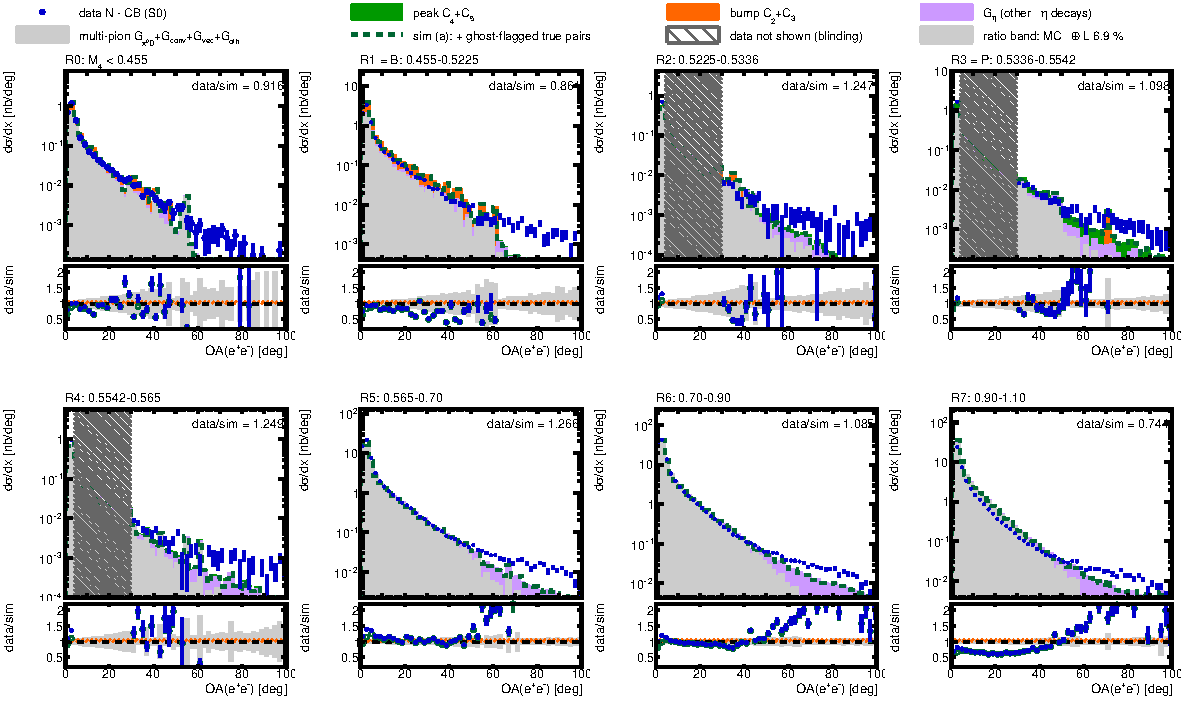
\includegraphics[width=0.86\textwidth]{figs_all/wp1_B4_oa.pdf}\\[0.2em]
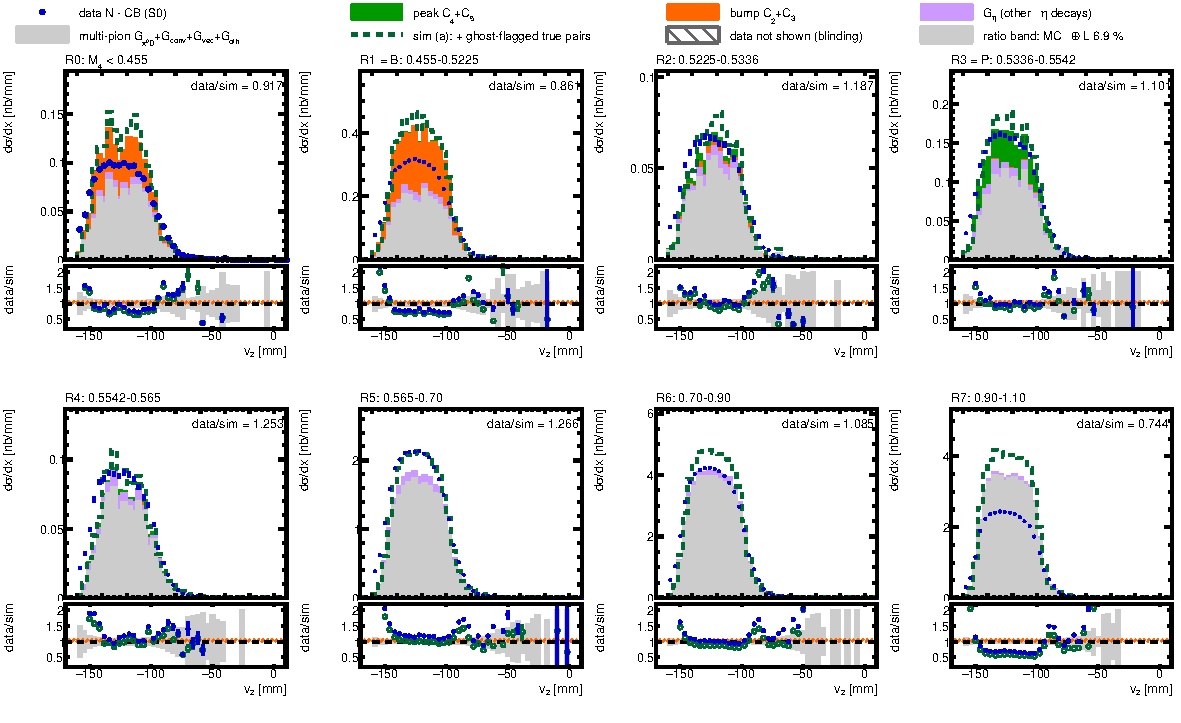
\includegraphics[width=0.86\textwidth]{figs_all/wp1_B4_vz.pdf}
\caption{\textbf{What it shows: the \ee opening angle and the event-vertex position, data against SMASH before any renormalisation, in each \Mfour region.}
Selection: data at $L=6079.2\,\nbinv$ with the nominal cuts S0 (PT3 trigger; event vertex in the target region, $\vz>-160$\,mm; START-free \betanew identification, pions within 3$\sigma$, leptons within 5$\sigma$ with a RICH ring; energy-loss-corrected momenta of all four tracks; both pions used in the event-vertex fit; all stored combinations of an event, isBest $\ge0$), in the \Mfour regions R0 (below 0.455), R1 (0.4550--0.5225, bump window), R2 (0.5225--0.53364), R3 (0.53364--0.55416, peak window), R4 (0.55416--0.565), R5 (0.565--0.70), R6 (0.70--0.90), R7 (0.90--1.10\,\GeVcc); data $(N-\mathrm{CB})\times64/63/L$, CB $=2\sqrt{N_{++}N_{--}}$ of the like-sign data per region ($k=1$) shared over the bins by their like-sign share; in R2--R4 the data at OA 4--30$^\circ$ are hidden. Simulation: SMASH $T_1+T_2$ ($\eta$ signal and physical background: a true \ee pair from one source), same cuts, mode A, $w\times$V3, \Mfour$\times0.99615$, \Mpipi$\times0.9952$, $\sum w/221.05\,\nbinv$.
Spec.\ Fig.~B4 (continued): opening angle OA (top) and vertex $z$ (bottom) in the regions R0--R7, S0. In R2--R4 the data OA in 4--30$^\circ$ are not drawn
(an X17 near 17\,\MeVcc would sit there). Colours, normalisation and errors as in Fig.~\ref{fig:B4}. No fall-back involved.}
\label{fig:B4b}
\end{figure}

\begin{figure}[H]
\centering
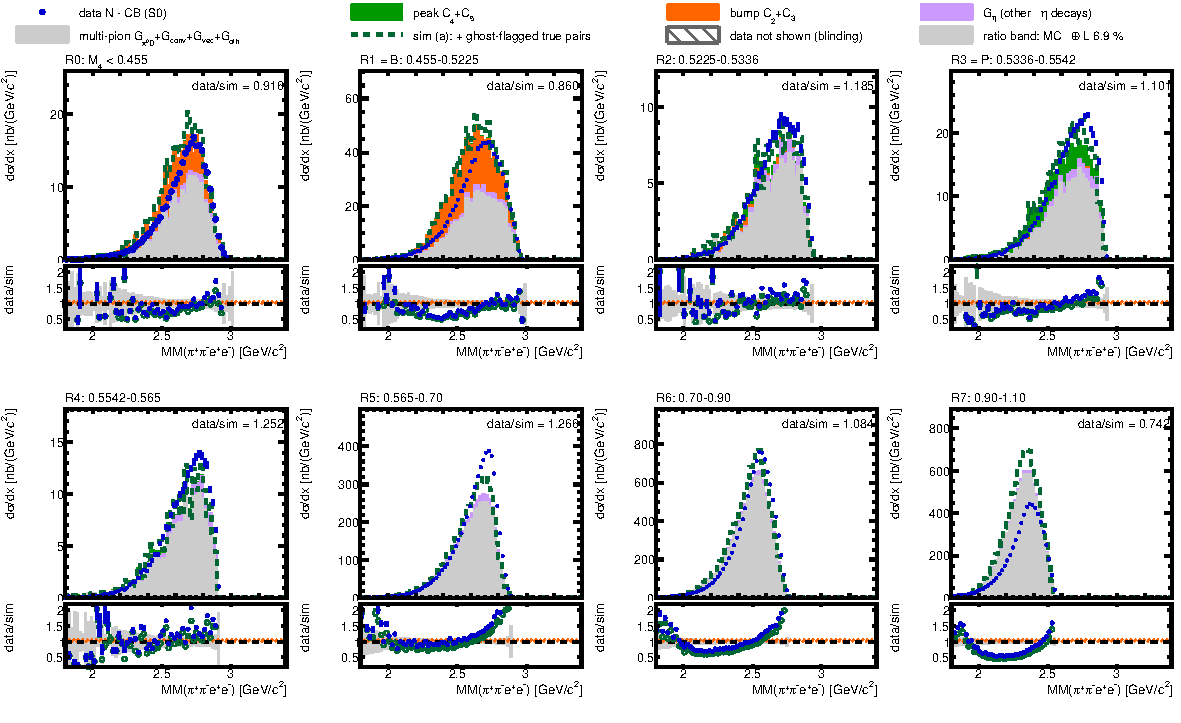
\includegraphics[width=0.92\textwidth]{figs_all/wp1_B4_mm4.pdf}\\[0.2em]
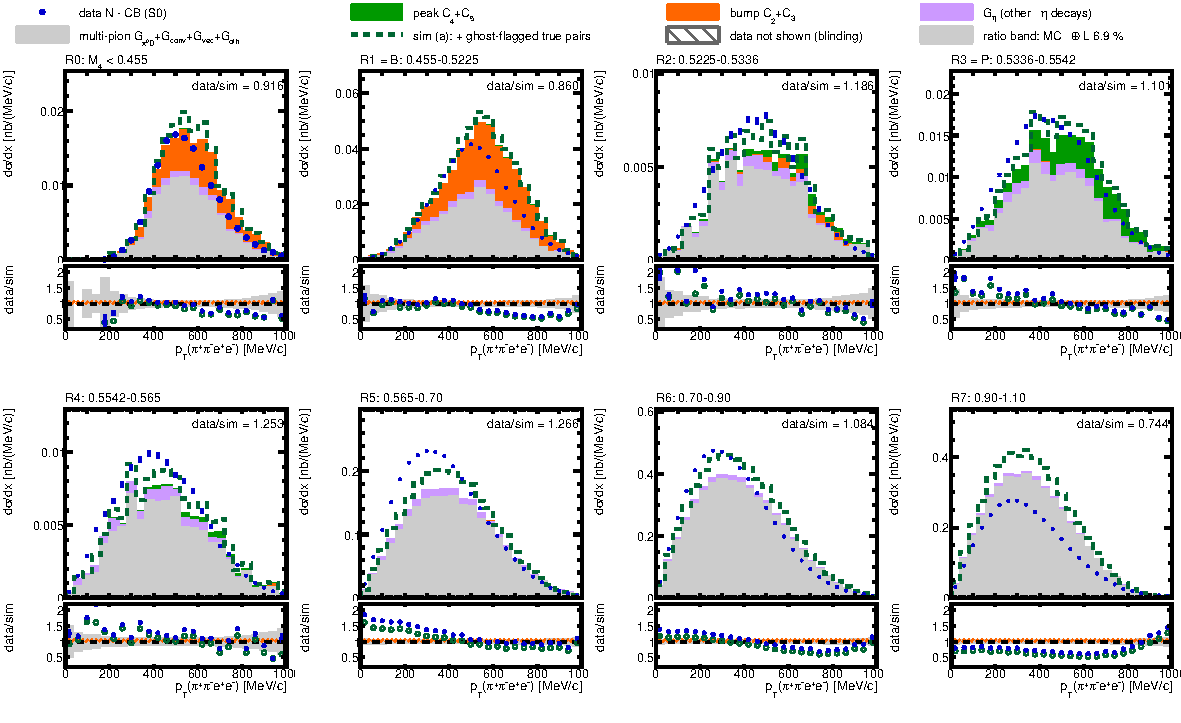
\includegraphics[width=0.92\textwidth]{figs_all/wp1_B4_pt4.pdf}
\caption{\textbf{What it shows: missing mass and transverse momentum of \ppee, data against SMASH before any renormalisation, in each \Mfour region.}
Selection: data at $L=6079.2\,\nbinv$ with the nominal cuts S0 (PT3 trigger; event vertex in the target region, $\vz>-160$\,mm; START-free \betanew identification, pions within 3$\sigma$, leptons within 5$\sigma$ with a RICH ring; energy-loss-corrected momenta of all four tracks; both pions used in the event-vertex fit; all stored combinations of an event, isBest $\ge0$), in the \Mfour regions R0 (below 0.455), R1 (0.4550--0.5225, bump window), R2 (0.5225--0.53364), R3 (0.53364--0.55416, peak window), R4 (0.55416--0.565), R5 (0.565--0.70), R6 (0.70--0.90), R7 (0.90--1.10\,\GeVcc); data $(N-\mathrm{CB})\times64/63/L$, CB $=2\sqrt{N_{++}N_{--}}$ of the like-sign data per region ($k=1$) shared over the bins by their like-sign share. Simulation: SMASH $T_1+T_2$ ($\eta$ signal and physical background: a true \ee pair from one source), same cuts, mode A, $w\times$V3, \Mfour$\times0.99615$, \Mpipi$\times0.9952$, $\sum w/221.05\,\nbinv$; missing mass at the beam kinetic energy 4530\,MeV (data) and 4500\,MeV (SMASH).
Spec.\ Fig.~B4 (continued): missing mass \MMfour (top; data at 4530\,MeV, simulation at 4500\,MeV, so the ratio contains the beam-energy difference) and
$p_{T,4}$ (bottom) in the regions R0--R7, S0. As Fig.~\ref{fig:B4}. No fall-back involved.}
\label{fig:B4c}
\end{figure}

\begin{figure}[H]
\centering
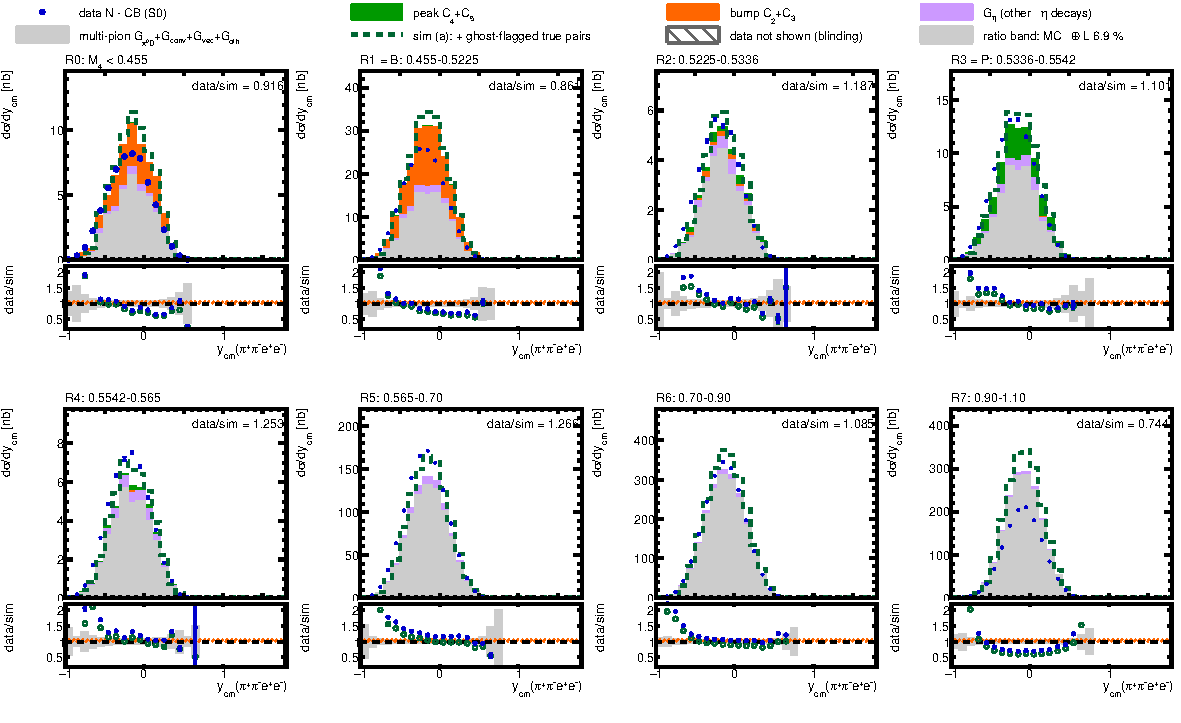
\includegraphics[width=0.75\textwidth]{figs_all/wp1_B4_y4.pdf}
\caption{\textbf{What it shows: the c.m.\ rapidity of \ppee, data against SMASH before any renormalisation, in each \Mfour region.}
Selection: data at $L=6079.2\,\nbinv$ with the nominal cuts S0 (PT3 trigger; event vertex in the target region, $\vz>-160$\,mm; START-free \betanew identification, pions within 3$\sigma$, leptons within 5$\sigma$ with a RICH ring; energy-loss-corrected momenta of all four tracks; both pions used in the event-vertex fit; all stored combinations of an event, isBest $\ge0$), in the \Mfour regions R0 (below 0.455), R1 (0.4550--0.5225, bump window), R2 (0.5225--0.53364), R3 (0.53364--0.55416, peak window), R4 (0.55416--0.565), R5 (0.565--0.70), R6 (0.70--0.90), R7 (0.90--1.10\,\GeVcc); data $(N-\mathrm{CB})\times64/63/L$, CB $=2\sqrt{N_{++}N_{--}}$ of the like-sign data per region ($k=1$) shared over the bins by their like-sign share. Simulation: SMASH $T_1+T_2$ ($\eta$ signal and physical background: a true \ee pair from one source), same cuts, mode A, $w\times$V3, \Mfour$\times0.99615$, \Mpipi$\times0.9952$, $\sum w/221.05\,\nbinv$; rapidity at the beam kinetic energy 4530\,MeV (data) and 4500\,MeV (SMASH).
Spec.\ Fig.~B4 (continued): c.m.\ rapidity $y_4$ in the regions R0--R7, S0 (data at 4530\,MeV, simulation at 4500\,MeV). As Fig.~\ref{fig:B4}. No fall-back involved.}
\label{fig:B4d}
\end{figure}

\begin{figure}[H]
\centering
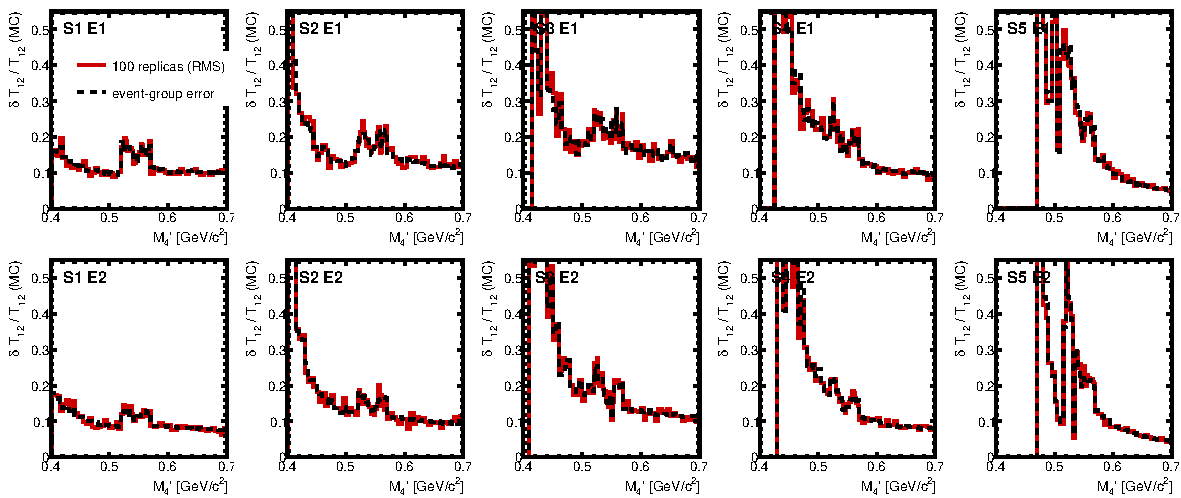
\includegraphics[width=0.78\textwidth]{figs_all/wp0_sim_mcerr.pdf}
\caption{\textbf{What it shows: the simulation-statistics error from the bootstrap replicas agrees with the event-group error (median ratio 0.99--1.02).}
Selection: simulation only, SMASH $T_1+T_2$ ($\eta$ signal and physical background: a true \ee pair from one source), mode A, $w\times$V3, \Mfour$\times0.99615$, \Mpipi$\times0.9952$, with the nominal cuts S0 (PT3 trigger; event vertex in the target region, $\vz>-160$\,mm; START-free \betanew identification, pions within 3$\sigma$, leptons within 5$\sigma$ with a RICH ring; energy-loss-corrected momenta of all four tracks; both pions used in the event-vertex fit; all stored combinations of an event, isBest $\ge0$); cells: five \Mpipi slices (below 0.34, 0.34--0.37, 0.37--0.39, 0.39--0.43, from 0.43\,\GeVcc) $\times$ \Mee below 10 and from 10\,\MeVcc, \Mfour 0.40--0.70\,\GeVcc in 70 bins (5\,\MeVcc; 2.5\,\MeVcc in 0.52--0.57).
Relative MC error of the simulated sum $T_1+T_2$ per F10 cell. S0, SMASH std + lep + $\eta$, mode A, $w\times$V3, $M_4'=0.99615\,M_4$. Red: rms of 100
Poisson event-group replicas; black dashed: event-group error. They agree (median ratio 0.99--1.02). No fall-back involved.}
\label{fig:mcerr}
\end{figure}

\begin{figure}[H]
\centering
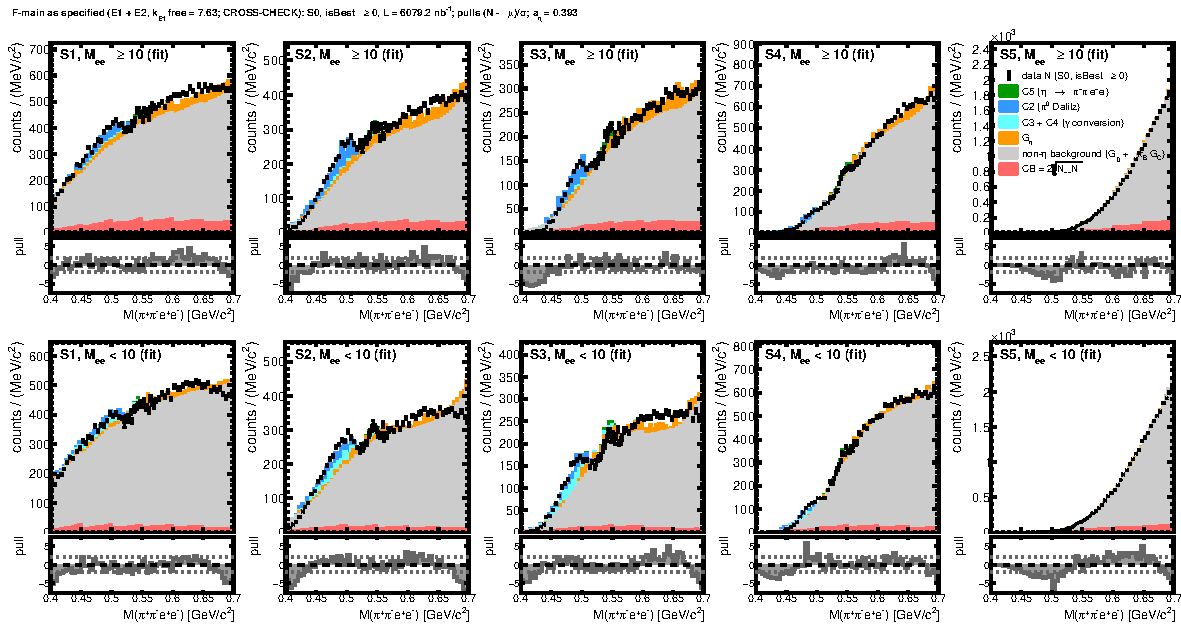
\includegraphics[width=0.70\textwidth]{figs_all/wp5_E1_spec_cnt.pdf}
\caption{\textbf{What it shows: the template fit F-main as first specified, with both \Mee classes fitted; it needs a CB factor of 7.6 below 10\,\MeVcc and was superseded by the fit without that class.}
Selection: data at $L=6079.2\,\nbinv$ with the nominal cuts S0 (PT3 trigger; event vertex in the target region, $\vz>-160$\,mm; START-free \betanew identification, pions within 3$\sigma$, leptons within 5$\sigma$ with a RICH ring; energy-loss-corrected momenta of all four tracks; both pions used in the event-vertex fit; all stored combinations of an event, isBest $\ge0$); both \Mee classes fitted, below 10 and from 10\,\MeVcc; the five \Mpipi slices (below 0.34, 0.34--0.37, 0.37--0.39, 0.39--0.43, from 0.43\,\GeVcc); \Mfour 0.40--0.70\,\GeVcc in 70 bins per histogram (5\,\MeVcc; 2.5\,\MeVcc in 0.52--0.57); CB $=2\sqrt{N_{++}N_{--}}$ of the like-sign data with the same cuts, shared over the cells by their like-sign share, times a factor fitted within $1\pm0.05$ from 10\,\MeVcc and free below; SMASH with the same cuts (mode A, $w\times$V3, \Mfour$\times0.99615$, \Mpipi$\times0.9952$).
F-main as specified (E1+E2, $\kEone=7.6$ free), pulls in both rows (CROSS-CHECK; superseded by the E1 fall-back). As Fig.~\ref{fig:E1}.}
\label{fig:E1spec}
\end{figure}

\begin{figure}[H]
\centering
\begin{subfigure}{0.38\textwidth}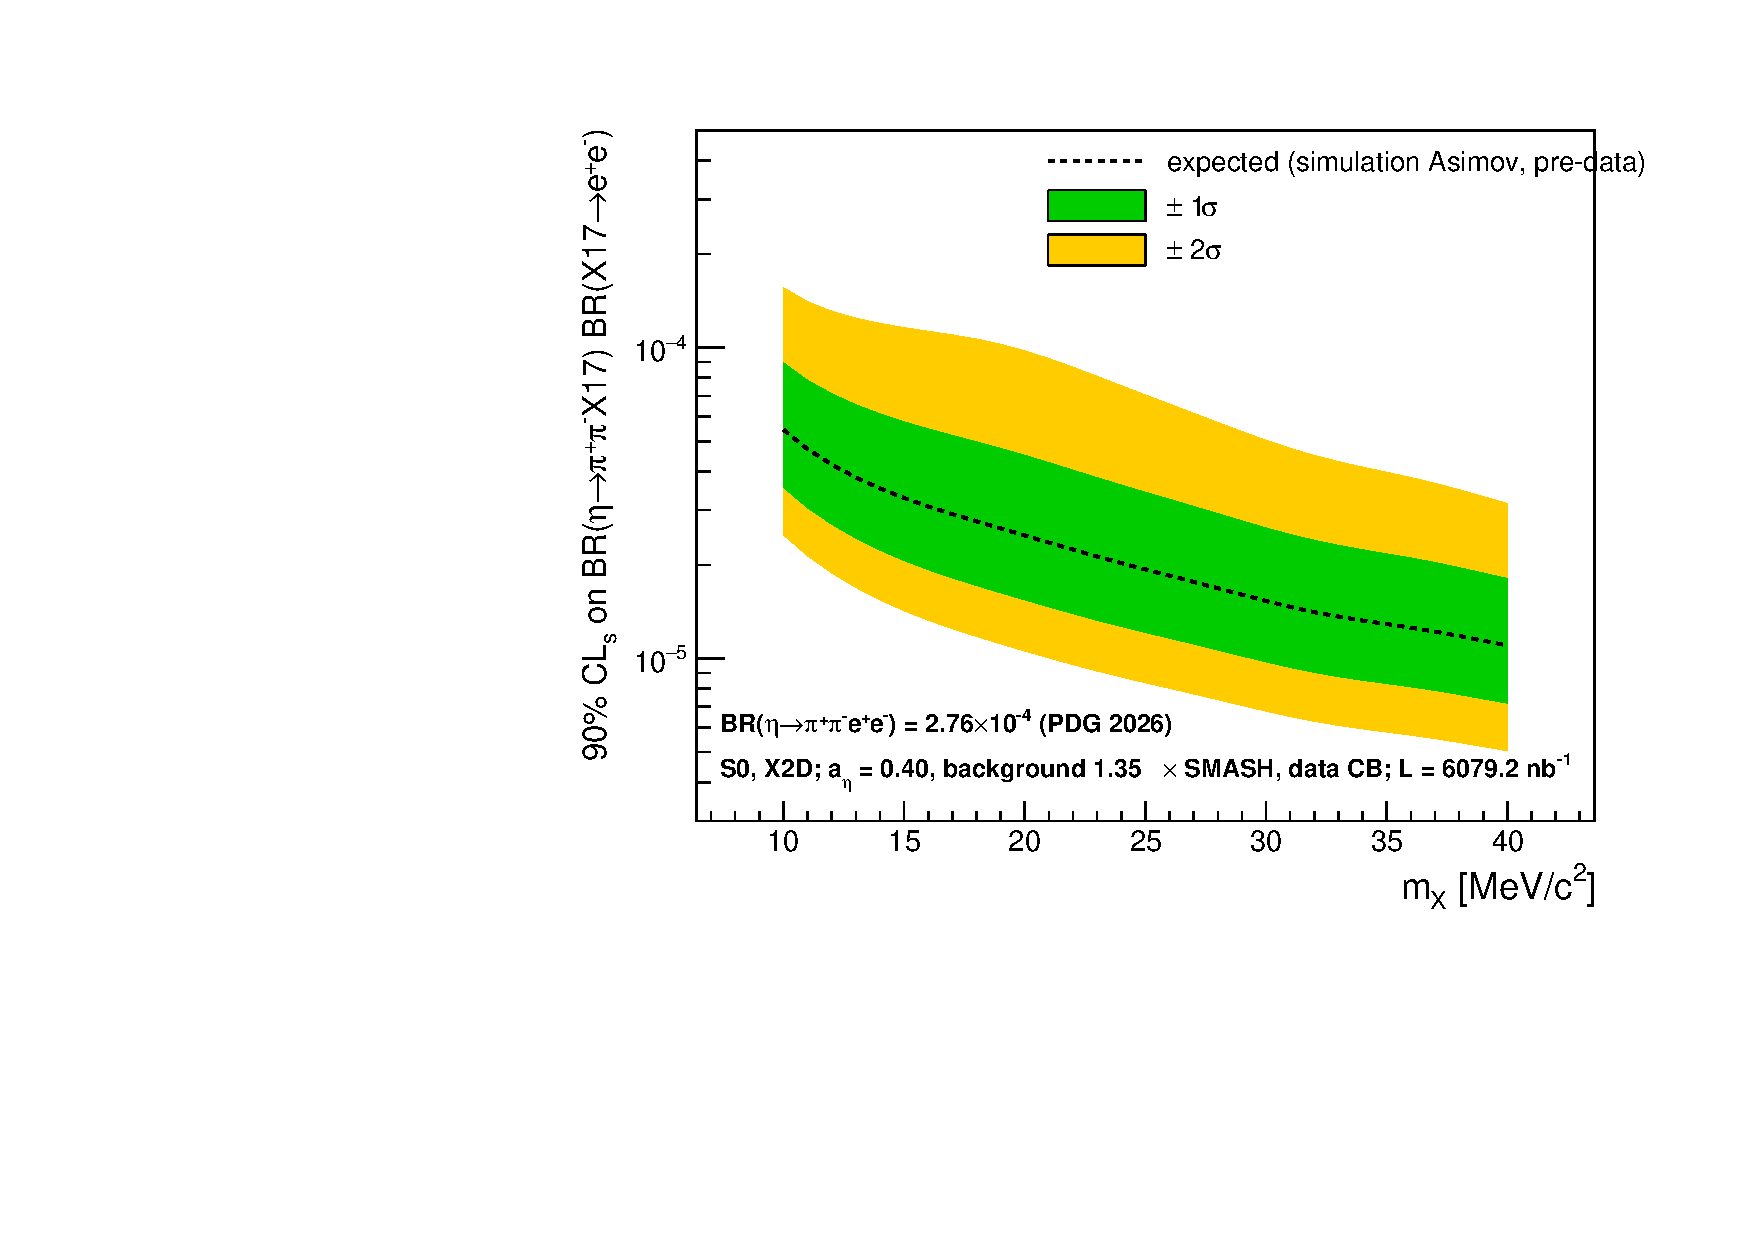
\includegraphics[width=\textwidth]{figs_all/x17ab_proj_mass_pdg26.pdf}\caption{}\end{subfigure}
\begin{subfigure}{0.38\textwidth}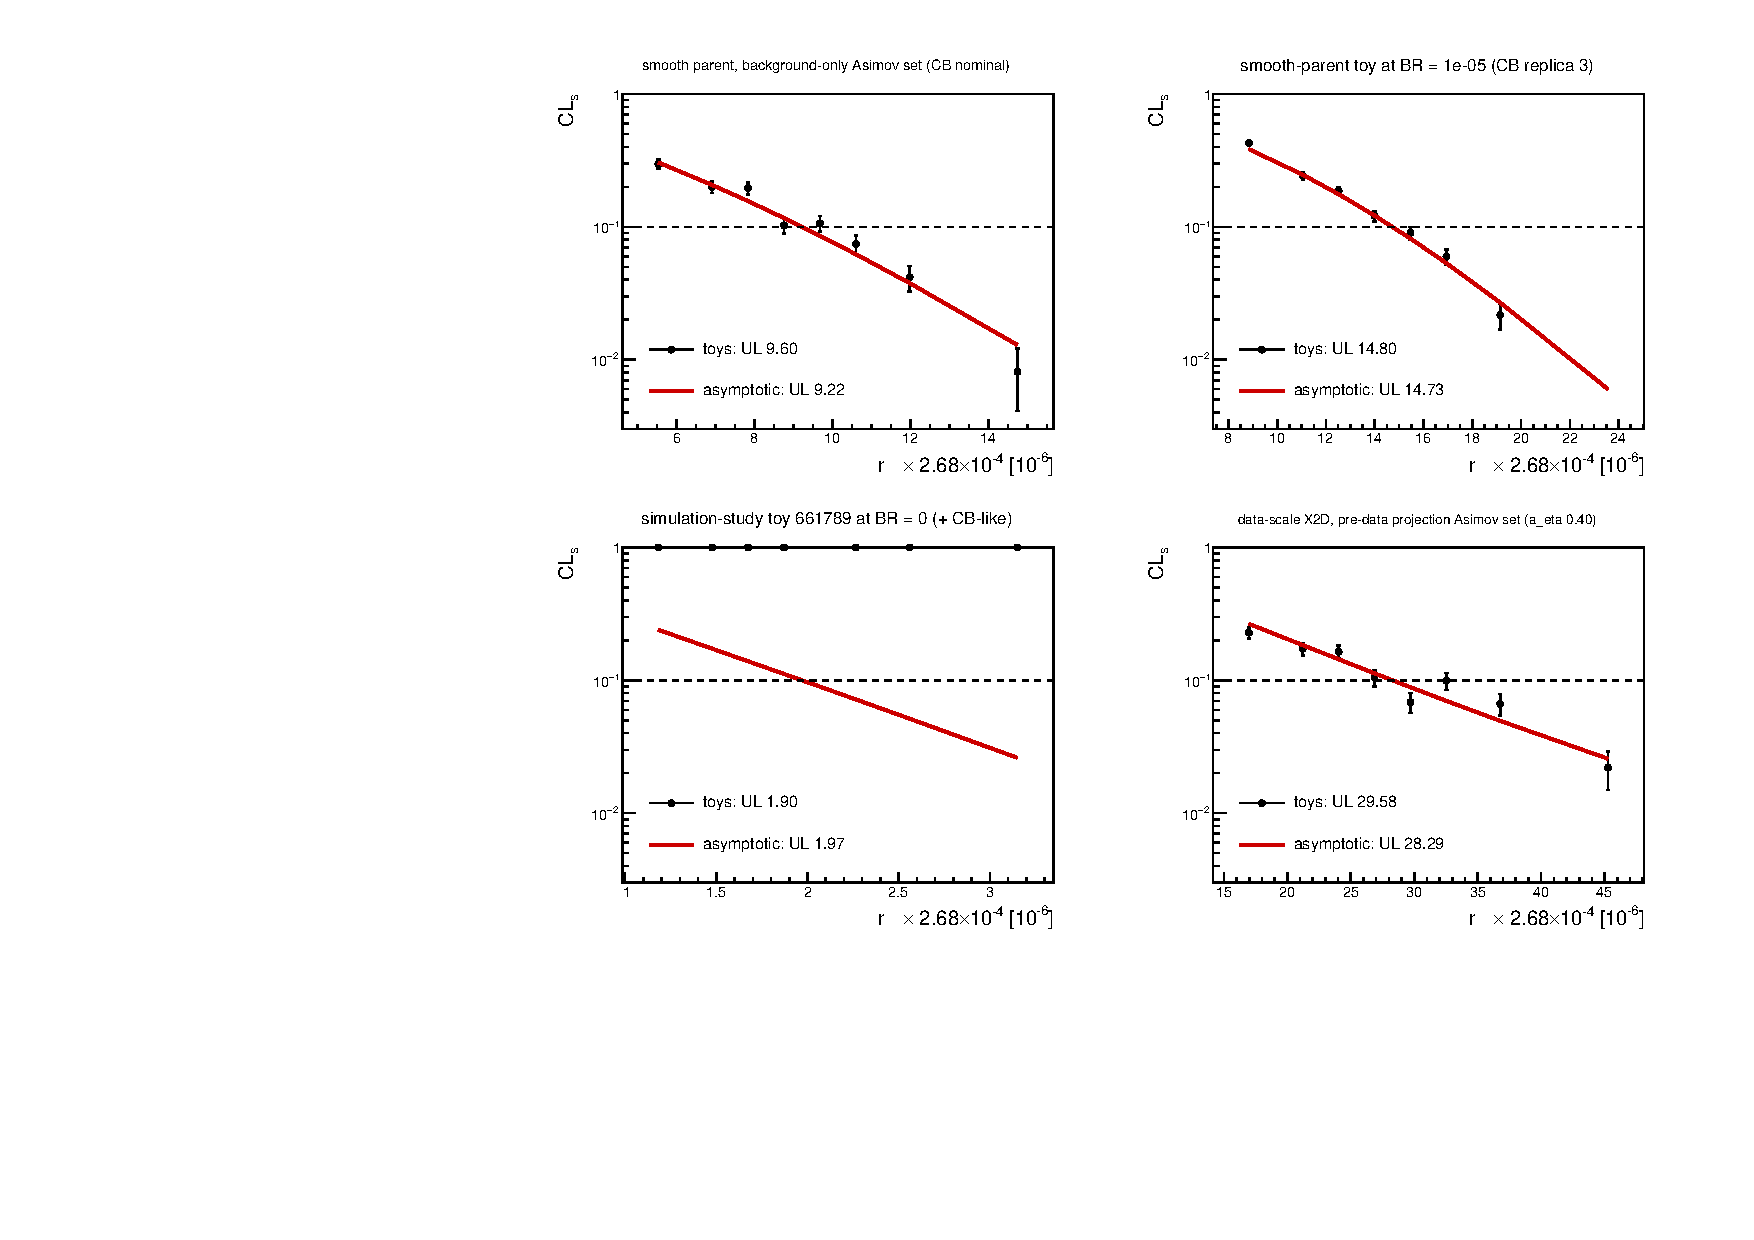
\includegraphics[width=\textwidth]{figs_all/x17ab_toycls.pdf}\caption{}\end{subfigure}
\caption{\textbf{What it shows: before any data were used, the expected limit against $m_X$ from a simulated data set, and toy against asymptotic CL$_s$ on four pseudo-data sets.}
Selection: no measured unlike-sign counts. (a) A simulated Asimov set in the plane \Mfour 0.5225--0.6100\,\GeVcc (35 bins of 2.5\,\MeVcc) $\times$ \Mee 2--62\,\MeVcc (30 bins of 2\,\MeVcc), with the nominal cuts S0 (PT3 trigger; event vertex in the target region, $\vz>-160$\,mm; START-free \betanew identification, pions within 3$\sigma$, leptons within 5$\sigma$ with a RICH ring; energy-loss-corrected momenta of all four tracks; both pions used in the event-vertex fit; all stored combinations of an event, isBest $\ge0$): SMASH (mode A, $w\times$V3, simulated \Mfour$\times0.99615$) with the $\eta$ terms at $a_\eta=0.40$, the other background at $1.35\times$ SMASH ($G_D+G_C$) in each \Mee row, and the CB of the data. (b) Four pseudo-data sets of the validation: the smooth-parent Asimov set, one smooth-parent toy with BR $10^{-5}$, one simulation-study toy with BR 0 and the Asimov set of the projection in (a).
X17, before the data. (a) PRE-DATA projection (BR with PDG 2026, D25; 2.91 instead of 2.83 at 17\,\MeVcc) of the expected 90\,\% CL$_s$ limit against $m_X$ with $\pm1\sigma$/$\pm2\sigma$ bands (simulation Asimov
set: $\aEta=0.40$, background $1.35\times$ SMASH, data CB; $L=6079.2\,\nbinv$; S0, X2D); superseded by Fig.~\ref{fig:x17freeze}(b). (b) CL$_s$ against $r$ for
four data sets: toys (1000 per point and hypothesis, binomial errors) against the asymptotic formula (red); dashed: CL$_s=0.10$. No fall-back involved.}
\label{fig:x17pre}
\end{figure}

\begin{figure}[H]
\centering
\begin{subfigure}{0.49\textwidth}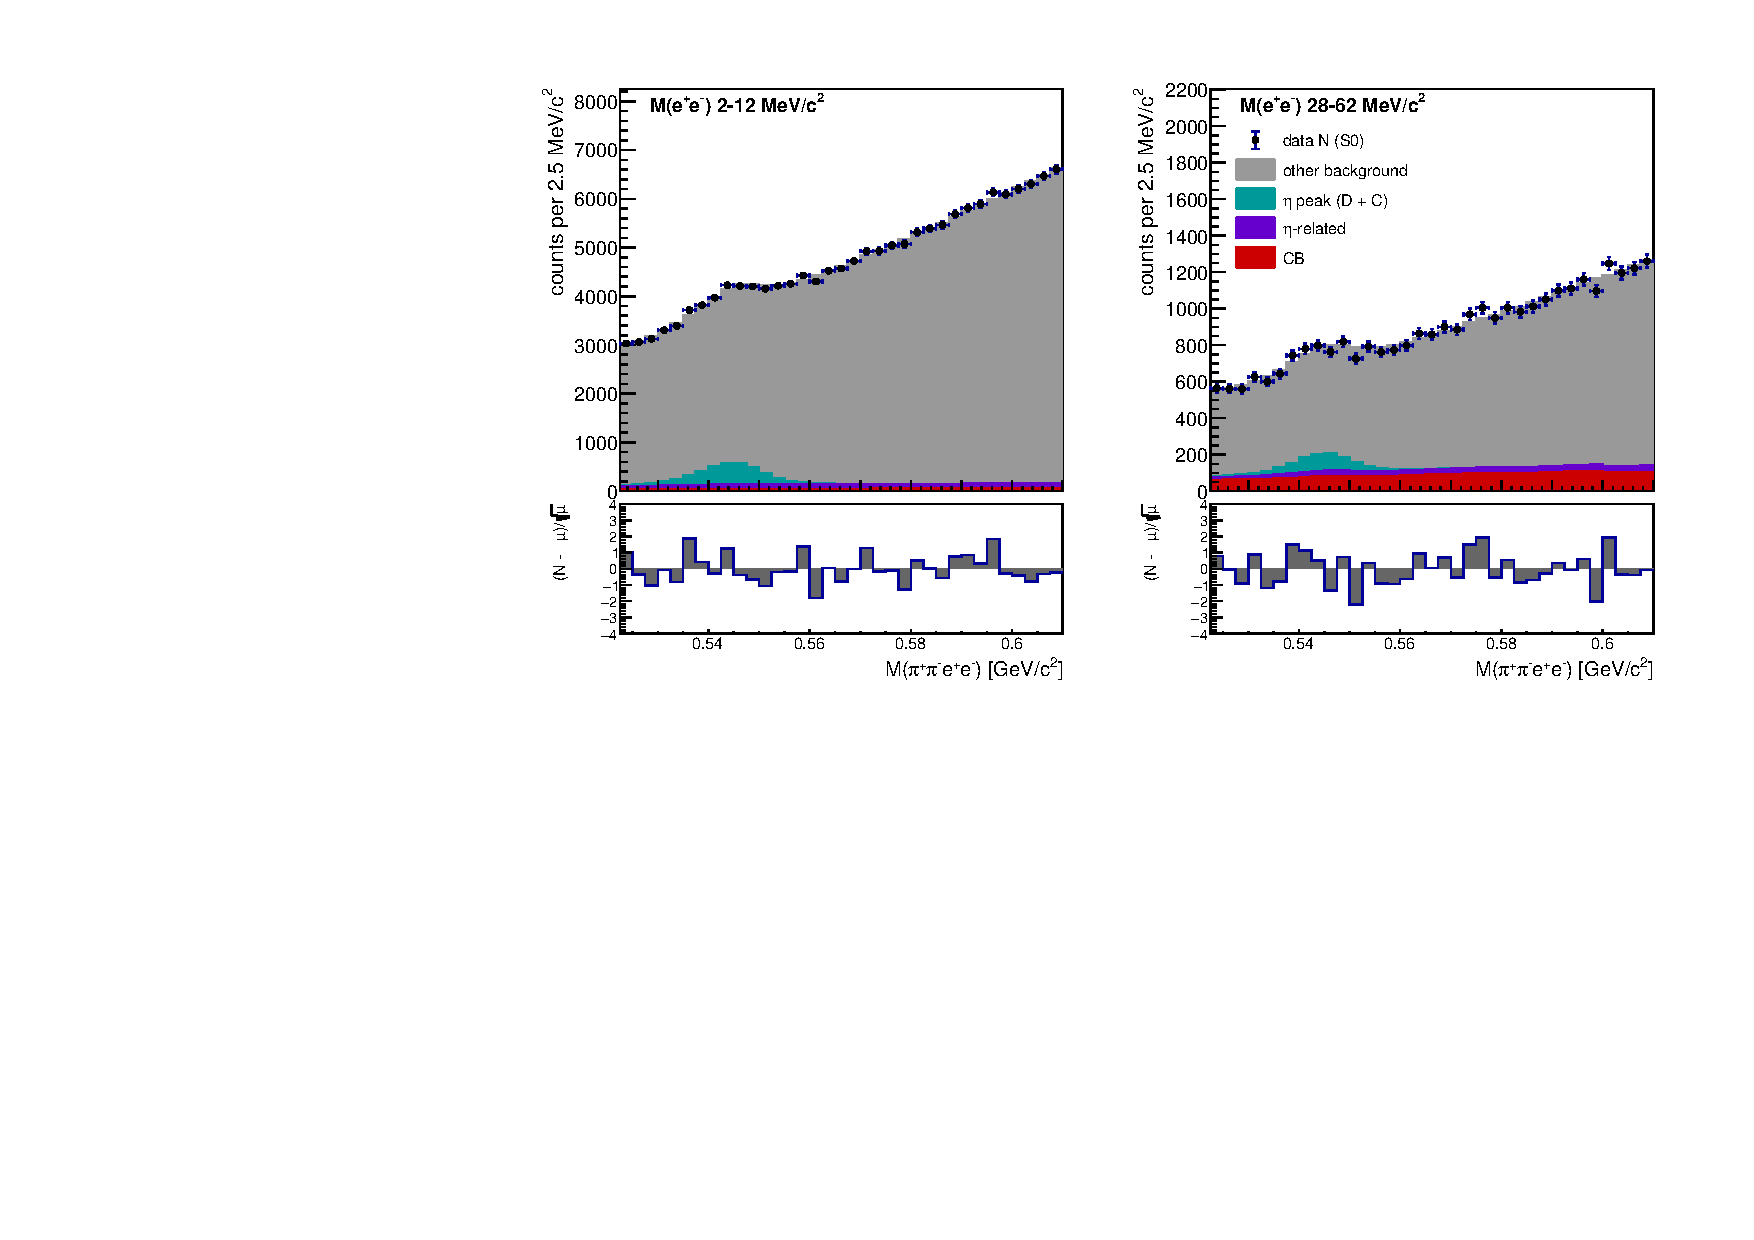
\includegraphics[width=\textwidth]{figs_all/x17c_sb_m4_cnt.pdf}\caption{}\end{subfigure}
\begin{subfigure}{0.49\textwidth}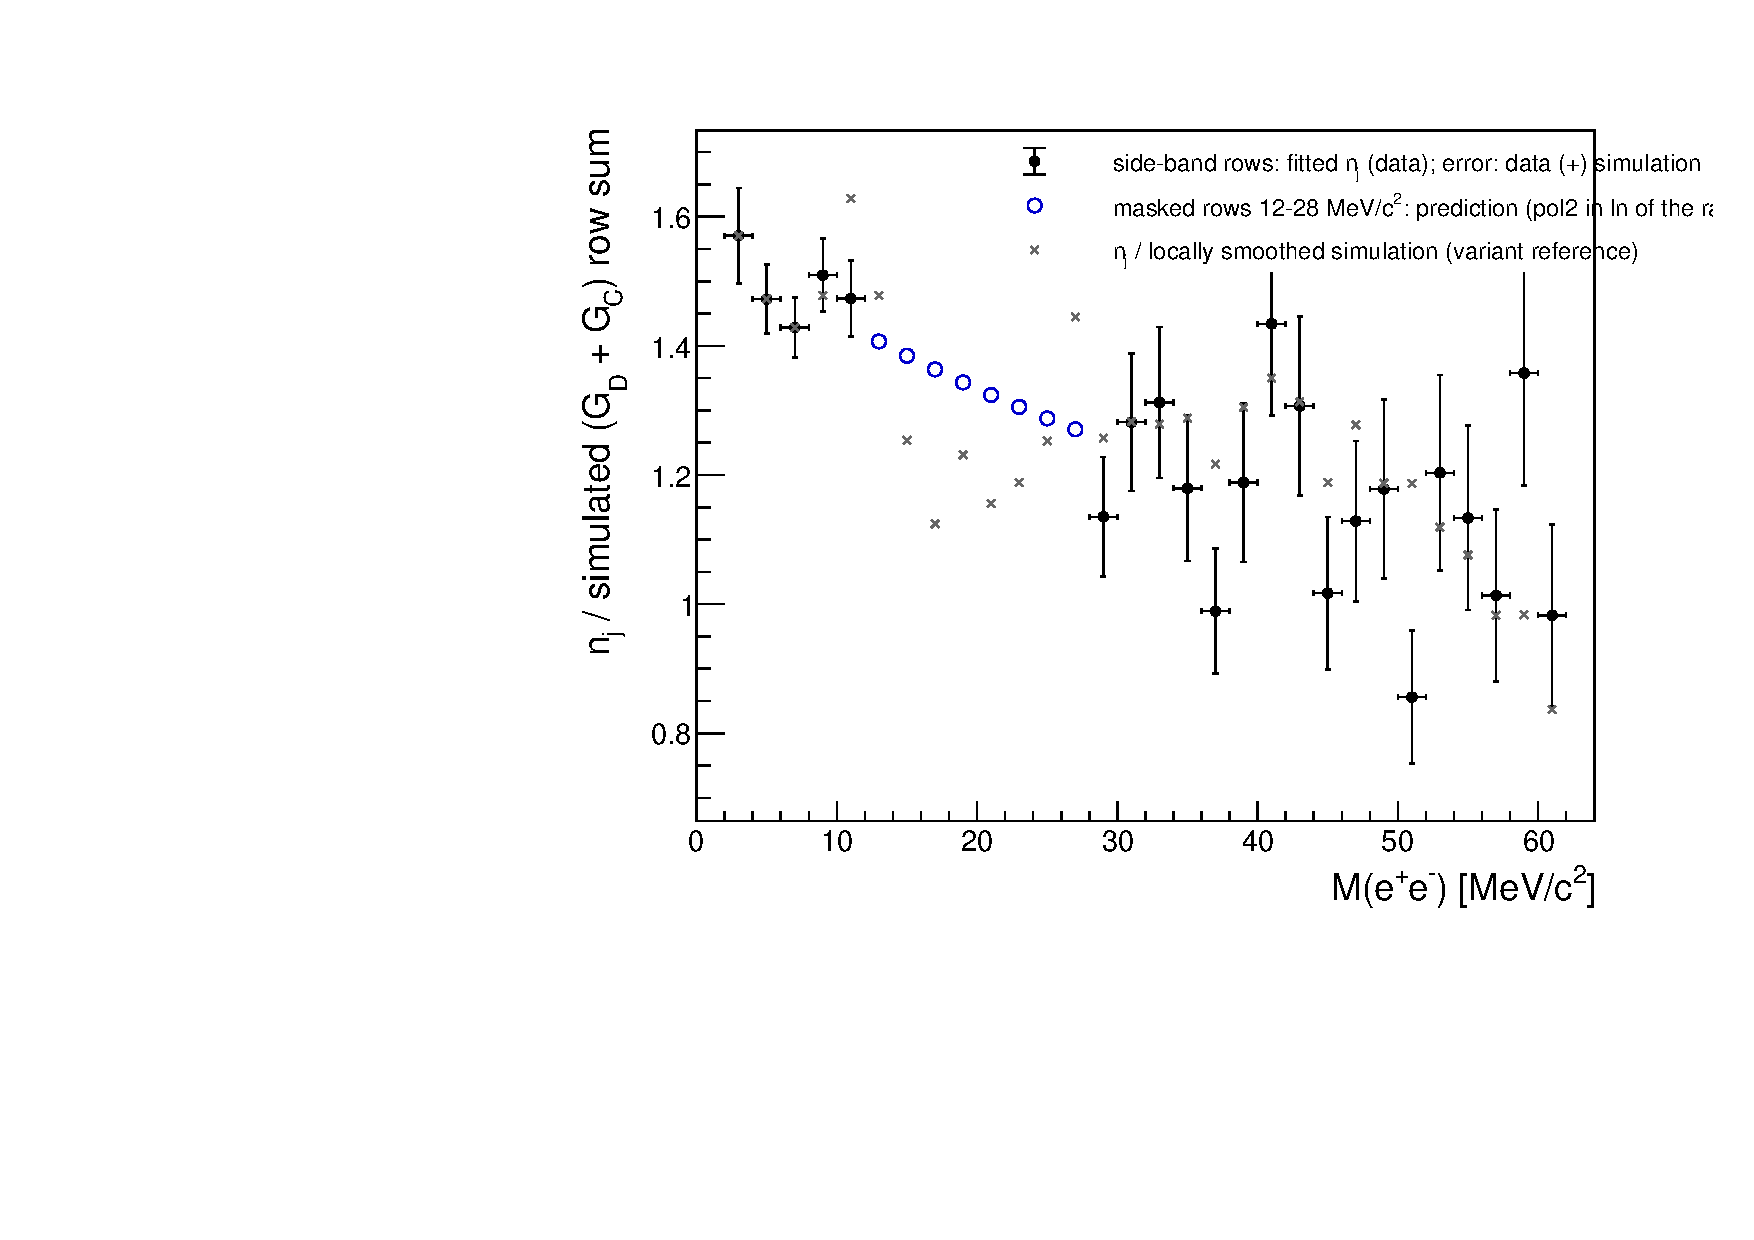
\includegraphics[width=\textwidth]{figs_all/x17c_fill.pdf}\caption{}\end{subfigure}\\
\begin{subfigure}{0.49\textwidth}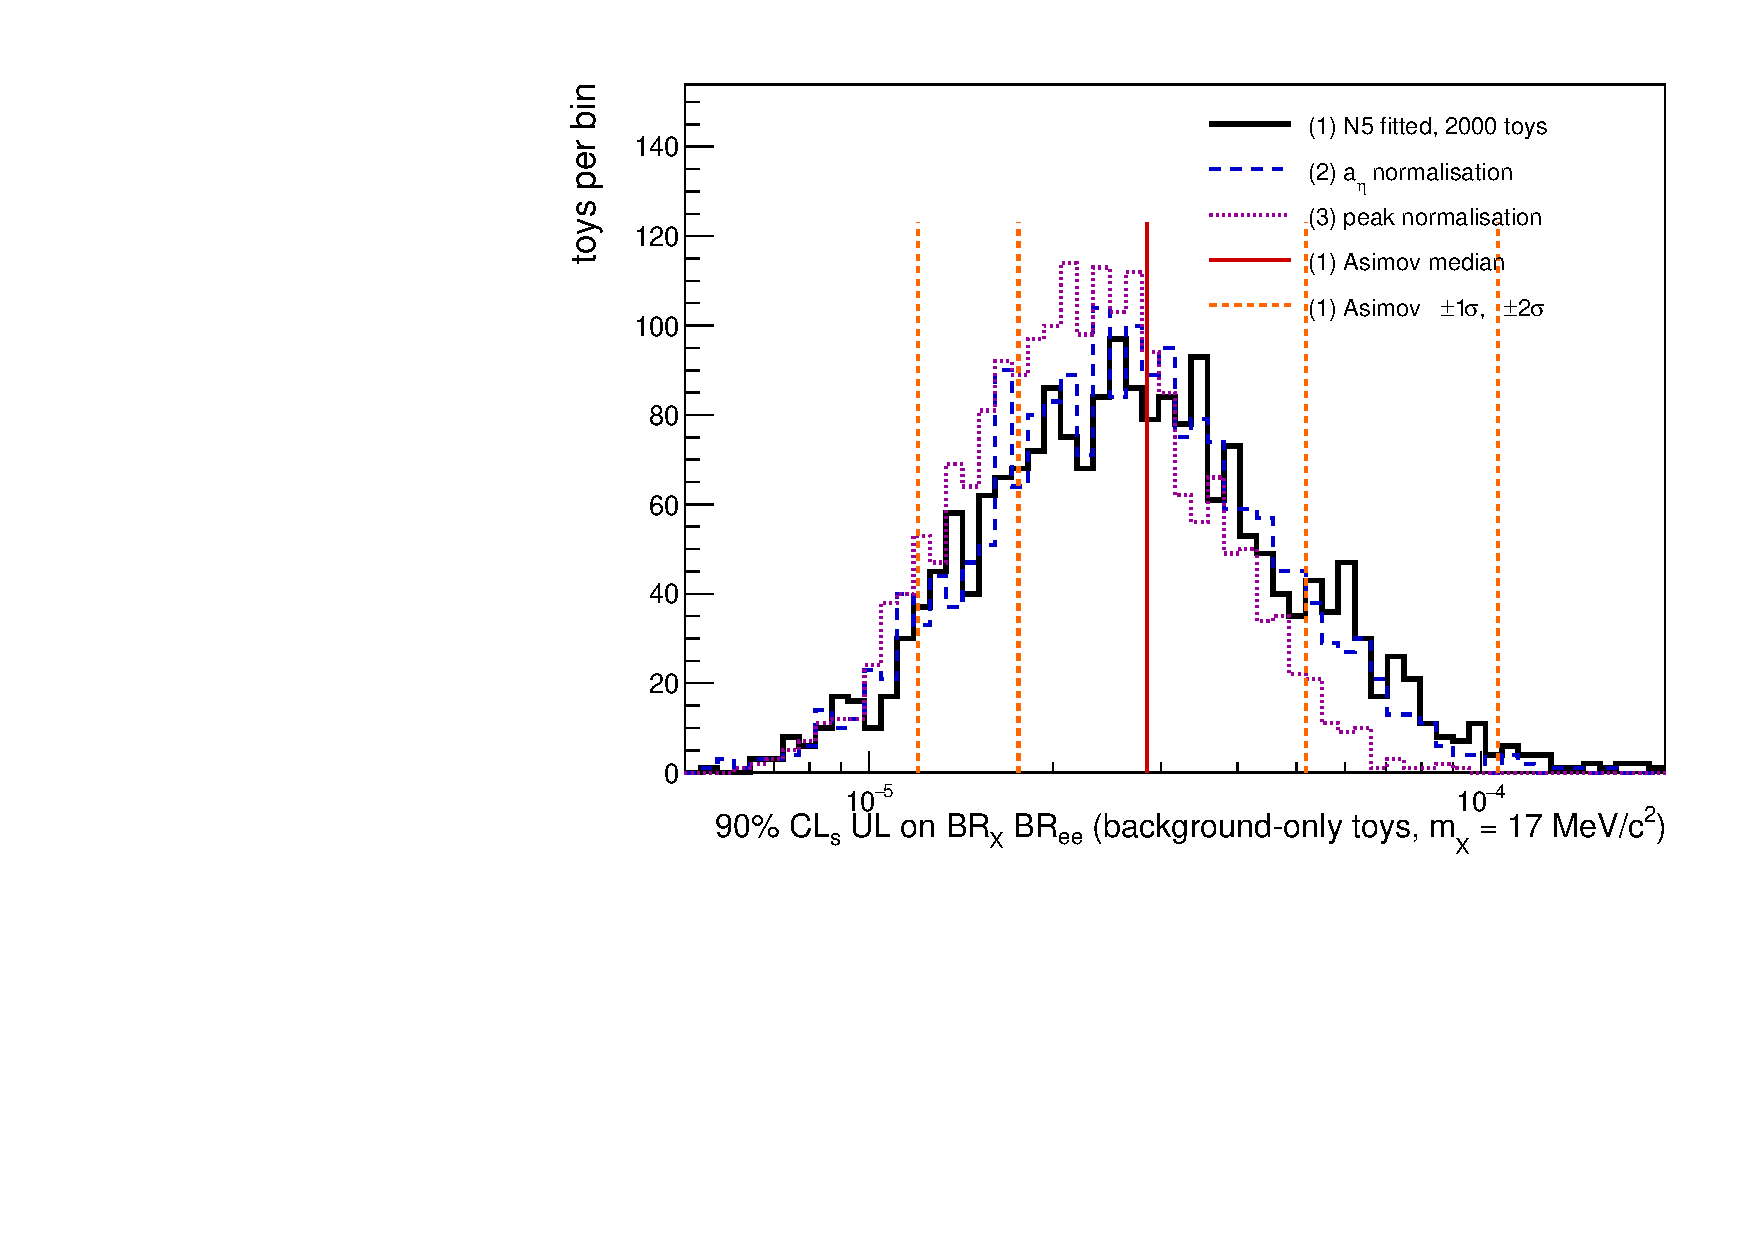
\includegraphics[width=\textwidth]{figs_all/x17c_toys_ul_pdg26.pdf}\caption{}\end{subfigure}
\begin{subfigure}{0.49\textwidth}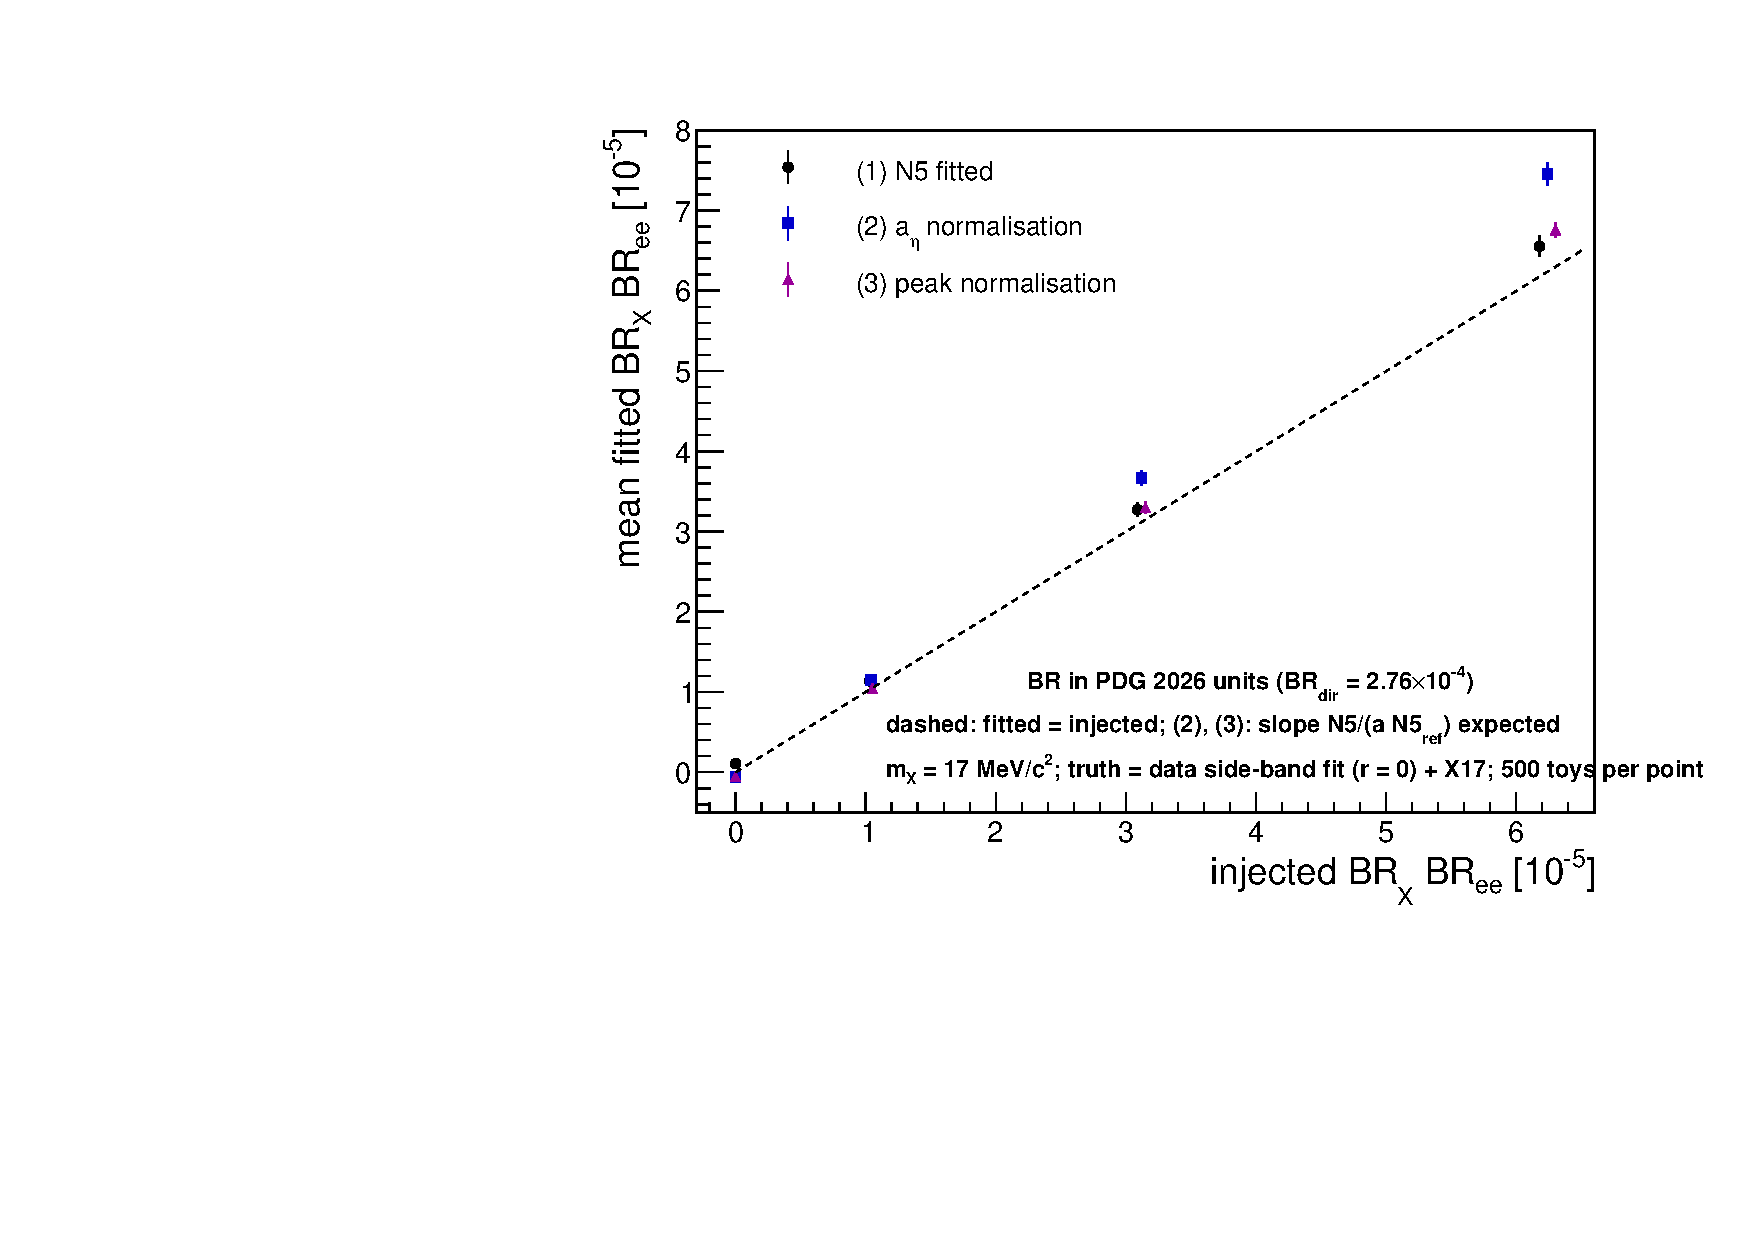
\includegraphics[width=\textwidth]{figs_all/x17c_inject_pdg26.pdf}\caption{}\end{subfigure}
\caption{\textbf{What it shows: the checks of the frozen side-band fit: its \Mfour projections, the background level per \Mee row with its prediction for the hidden rows, the spread of the expected limits, and the response to injected X17.}
Selection: (a), (b) data at $L=6079.2\,\nbinv$ with the nominal cuts S0 (PT3 trigger; event vertex in the target region, $\vz>-160$\,mm; START-free \betanew identification, pions within 3$\sigma$, leptons within 5$\sigma$ with a RICH ring; energy-loss-corrected momenta of all four tracks; both pions used in the event-vertex fit; all stored combinations of an event, isBest $\ge0$), \Mee side bands 2--12 and 28--62\,\MeVcc (\Mee 12--28\,\MeVcc hidden until the freeze) of the plane \Mfour 0.5225--0.6100\,\GeVcc (35 bins of 2.5\,\MeVcc) $\times$ \Mee 2--62\,\MeVcc (30 bins of 2\,\MeVcc); CB of the like-sign data with the same cuts (10\,\MeVcc cells of \Mfour, shared over the \Mee bins by the like-sign share of each 50\,\MeVcc band), its factor fitted within $1\pm0.5$ for \Mee$<10$\,\MeVcc and $1\pm0.05$ above; (a) \Mfour projections of the lower (2--12) and the upper (28--62\,\MeVcc) side band; (b) the fitted background normalisation of each 2\,\MeVcc row of \Mee over the simulated $G_D+G_C$ row sum (SMASH with the same cuts, mode A, $w\times$V3). (c) 2000 background-only toys and (d) 500 toys per point with X17 injected, both drawn from the side-band fit in the full plane.
X17 freeze (X-c). (a) \Mfour projections of the side bands (2--12 and 28--62\,\MeVcc) with the fitted components; lower panels $(N-\mu)/\sqrt\mu$;
Pearson $\chi^2$/ndf 749/730. (b) Fitted $n_j$ / simulated $G_D+G_C$ row sum (black; fit $\oplus$ simulation errors) and the prediction for the masked rows,
pol2 in the logarithm of the ratio (open blue); grey crosses: divided by the locally smoothed simulation (variant). (c) 90\,\% CL$_s$ limits of 2000
background-only toys at 17\,\MeVcc, normalisations (1) black, (2) blue, (3) magenta; vertical lines: Asimov median (red) and $\pm1/2\sigma$ (orange) of (1).
(d) Mean fitted against injected BR at 17\,\MeVcc (truth: side-band fit + X17 injected in normalisation (1), 500 toys per point); (2) and (3) read the same
counts with their own $\eta$ scale (expected slopes 1.185 and 1.093). BR axes of (c), (d) with PDG 2026 (D25). S0, isBest $\ge0$, $L=6079.2\,\nbinv$. No fall-back involved.}
\label{fig:x17c}
\end{figure}

%======================================================================
\section{Reconciliation: numbers corrected or superseded}
\label{app:recon}
%======================================================================
Where two sources disagree, this report uses the value of the later independent verification or of the binding amendment. The list (also in the
writer log):
{\footnotesize
\setlength{\tabcolsep}{3pt}
\renewcommand{\arraystretch}{1.08}
\begin{longtable}{@{}>{\raggedright\arraybackslash}p{3.6cm} >{\raggedright\arraybackslash}p{4.4cm} >{\raggedright\arraybackslash}p{4.4cm} >{\raggedright\arraybackslash}p{\dimexpr\textwidth-12.4cm-6\tabcolsep\relax}@{}}
\caption{\textbf{Superseded and corrected numbers.}}\label{tab:recon}\\
\toprule
quantity & original (source) & used here (source) & reason \\
\midrule
\endfirsthead
\toprule
quantity & original & used here & reason \\
\midrule
\endhead
\bottomrule
\endfoot
\sigeta & $0.437\pm0.037\pm0.070\pm0.026$\,mb (WP7, WP8) & $0.429\pm0.036\pm0.079\pm0.025$\,mb (v8) & PDG 2026, $\sigma_{\mathrm{SMASH}}$ 1.0694, \Csec(peak), peak composition \\
syst of \sigeta & 16.0\,\% (WP7/WP8) & 18.5\,\% (v8) & composition of the peak, $\kappa=1\pm0.2$ \\
\sigeta$/\sigma_{\mathrm{SMASH}}$ & $0.410\pm0.085$ (WP8) & $0.401\pm0.092$ (v8) & as above \\
\BRG, \BRA, DR, DR$_F$ & 2.65, 3.52, 1.397, 1.169 (PDG 2020) & 2.67, 3.54, 1.373, 1.148 (v8) & PDG 2026 rescaling \\
PDG reference of BR$(\eta\to\ppee)$ & $2.68\pm0.11\times10^{-4}$ (PDG 2020) & $2.76\pm0.16\times10^{-4}$ (PDG 2026) & current edition \\
$\eta$ normalisation & $\Csec(1-\fwin)=0.842$ (WP2) & $\Csec(1-\feta)=0.98$ (Amendment~1) & material not in the $\eta$ signal \\
\fwin(B+P) & $16.8^{+5.0}_{-5.9}$\,\% (WP2) & $14.7\pm1.1^{+1.0}_{-2.0}$\,\% (verification) & halo reweighting; composition only \\
spec.\ Table~P1 efficiencies & $\sigma_{\mathrm{SMASH}}=1.0665$\,mb & 0.28\,\% too high (v8) & simulated sample 1.0694\,mb \\
live time & $+7.3$\,\% & $+7.1$ to $+7.3$\,\% (v8) & $L$ weighting \\
literature & ``no published inclusive value'' (WP8) & HADES 3.5\,GeV $1.14\pm0.20$/$0.93\pm0.14$\,mb; Krak\'ow talk 1.15/1.72\,mb (v8) & missed reference; Staudenmaier over-interpreted \\
$f_\eta$(edge) stat & 0.020 (WP6) & 0.024 & Part~II calibration $\times1.2$ of the edge-step errors \\
\Pmain model & $\pm1078$ (old envelope) & $\pm420$ (Part~II edge-safe rms of ``pre + vertex'') & Part~II review \\
X17 $\sigma\times$BR$\times$BR & $<10.5$\,nb (x17d; $\sigma=0.343$\,mb with $1-\fwin$) & $<12.2$\,nb (vx, F-main $\sigma$); $<13.1$\,nb with the adopted 0.429\,mb (writer) & Amendment~1; adopted \sigeta \\
X17 $N_X^{\mathrm{UL}}$ & 563 counts (x17d: conversion of the BR limit) & 392--394 counts (vx: direct limit) & spec asks for a limit on counts \\
X17 MC column & $2.39\times10^{-6}$ (pooled replicas) & $3.34\times10^{-6}$ (CB $\oplus$ C4, vx) & independent sources \\
WP5 resolution statement & ``$r_{\mathrm{res}}=1.10$ consistent with D8'' & opposite to D8; no preference in the peak region (v5) & text error \\
free $s$ & PASS (WP5) & MARGINAL, minimum not bracketed (v5) & \\
WP5 error scale & 1.61 (GLS with replicas) & 1.38 (hybrid GLS, v5) & replica covariance rank 99 \\
spec.\ Fig.~E2 & \code{wp5_E2.pdf} (legend hides S5 data) & \code{v5_wp5_E2_corrected.pdf}, recoloured \code{fix_E2.pdf} & v5, review \\
WP1 acceptance references & 0.958 / 1.233 / 1.44--1.47 (spec) & valid for $s=1$; with D8 0.949 / 1.212 / 1.431 & mass transfer \\
D19 ``CB 112'' & 112 (geometric mean of X17P) & $171\pm6$ (spread rule) & CB construction \\
data-only $S$, $E$ (Part~II) & old envelope; $E$ fit error & PEAK $4364\pm310\pm477$, pre $4671\pm367\pm453$; $E=1199\pm85\pm287$ (later $\pm71$: the bootstrap confirms the fit error) & Part~II review \\
\multicolumn{4}{@{}l}{\emph{Review of this report}} \\
syst of \sigeta & 18.5\,\% (v8, prior $\kappa=1\pm0.2$) & 35.5\,\% (composition from the data, $\pm31.8$\,\%) & prior is a fall-back number; data give $\kappa\approx0.4$--0.5 \\
\sigeta$/\sigma_{\mathrm{SMASH}}$; total & $0.401\pm0.092$; 22.9\,\% & $0.401\pm0.152$; 37.9\,\% & as above \\
``about $3\sigma$ below'' 3.5\,GeV & status box, \S\ref{sec:lit}, conclusions & no significance (``lower value'' also dropped in the final review) & one-sided items missing; known-sign items of the same size \\
\sigeta cross-checks & 0.400 / 0.410 / 0.475 / 0.422\,mb (PDG 2020, 1.0665) & 0.399 / 0.409 / 0.474 / 0.414 (0.372 at $r_{\mathrm{res}}=0.89$) & one PDG edition and $\sigma_{\mathrm{SMASH}}$ \\
SMASH visible & 2.001 / 9.008\,nb & 2.046 / 9.047\,nb & PDG 2026 \\
$a_B$, DR & ``$a_B=0.312$'', DR $=\aP/a_B$ & $a_B(E2)=0.312$, $a_B(\mathrm{all})=0.299$, DR $=\aP/a_B(\mathrm{all})$ & definition; $\kappa$ convention \\
$\sigma\times$BR$(\eta\to\pipi\piz)$ & 75\,$\mu$b (``from B4'', 1.0665, mean \Csec) & 72 / 75\,$\mu$b ($a_B(\mathrm{all})$ / $a_B(E2)$), not determined & definition \\
B4 labels & ``MAIN'', ``main; WP4 fail'' & main bump estimator by fall-back, NOT DETERMINED; DR not determined & 157--165\,\% syst \\
X17 BR conversion & $r\times2.68\times10^{-4}$, edition not stated & PDG 2020 frozen; 3.16 with PDG 2026; $r_{\mathrm{UL}}=0.114$ & D25 \\
X17 $\sigma\times$BR$\times$BR & $<13.1$\,nb (plain product) & $<15.0$\,nb (\sigeta folded, log-normal) & \code{fix_x17_fold.py} \\
X17 68\,\% band (notebox) & $[1.50,4.84]$ (two masses) & $[1.50,4.77]$ at 17.0\,\MeVcc & transcription \\
stage-A $\chi^2$ & GLS 1.10 (rank-99 replica covariance) & hybrid 1.21--1.24; M1$\to$M2 $\Delta\chi^2$ 4.2--4.5 & \code{fix_stageA_gls.py} \\
A3 & PASS & FAIL for the \Geta content & 0.68$\sigma$ $>$ 0.3$\sigma$ \\
$\sigma_{\mathrm{tr}}$ & 239 counts & $239^{+254}_{-239}$; $\sigma_{\mathrm{tr}}(E2)=395$ & overlapping windows \\
S8 & \Ybump 4.5\,\%, \Ypeak 0.3\,\% & 7.7\,\%, 1.0\,\% & $g$ range 0.47--2.6 \\
fold $z$ (\S\ref{sec:cons}) & $-1.69$ / $-1.57$ / $-1.71$ (WP5) & $-1.37$ / $-1.22$ / $-1.55$ (WP7) & printed errors \\
$R_{34}$ errors & $\pm0.19\pm0.29$, E2 $\pm5.6$ (WP8) & $\pm0.18\pm0.24$ (total 0.30), E2 $\pm4.8$ (WP5) & spec.\ Table~E2 \\
$f_\eta$(edge) per class stat & E1 0.024, E2 0.036 & 0.029, 0.043 & $\times1.2$ calibration \\
\Pmain like for like & 0.403 & 0.403 ($r_{\mathrm{res}}=1$), 0.363 ($r_{\mathrm{res}}=0.89$) & data width \\
ghost variant & ``lowers every ratio by 9--16\,\%'' & lowers by 8.5--14.5\,\% ($J$ 6.6\,\%); simulation $+9$--17\,\% & spec.\ Table~B1 \\
material share & 12--15\,\% / 13--15\,\% & 13--15\,\% & Amendment~1 \\
ECAL tag & ``reproduces Part~II exactly'' & 3090 vs Part~II 3088 (2 counts) & wording \\
E1 prediction & ``0.75--0.90 of the data'' & data are 0.75--0.90 of the prediction & inverted \\
\Ypeak syst & 11.4\,\% & 11.5\,\% (S8 widened) & S8 \\
f$_\eta$ reason & ``would remove the material twice'' & \fwin describes the non-$\eta$ background & reasoning \\
\multicolumn{4}{@{}l}{\emph{Vertex study (after the review), \S\ref{sec:vertexeff}}} \\
$\eta$ efficiency of $\vz>-500$\,mm & not measured; ``up to $\times1.4$--1.7'' (survival of the counts 0.565 in P, 0.68 of $N-\mathrm{CB}$) & $0.994\pm0.021$ (data), 0.9997 (simulation); $C_{\mathrm{vtx}}=1.006\pm0.021$, one-sided $+2$\,\% & measured (ve\_verify) \\
simulated vertex survival & $\ge0.96$ (0.968 / 0.976 / 0.959) & 0.99970 (C4+C5), 0.9986 (C2+C3) & the old numbers were FAT/PAT entry ratios of whole sets \\
\sigeta with the one-sided items & 0.67--0.82\,mb; 0.81--1.19\,mb (direct route); up to 1.44\,mb (with $p_T$) & 0.48\,mb; direct route 0.58--0.59\,mb (0.70\,mb per-class side bands); up to 0.85\,mb & no vertex factor; route values apart \\
status box / conclusions & ``could be 0.7--1.2\,mb, the tension would disappear'' & 0.48 (0.58--0.59; 0.70)\,mb; the one-sided items alone do not remove the difference; with the side-band route value and the $p_T$ item 0.85\,mb, compatible with 0.93\,mb & vertex measured \\
X17 $\sigma\times$BR$\times$BR & ``21--26\,nb at the $N-\mathrm{CB}$ / raw-count rate'' & 15.1\,nb with $C_{\mathrm{vtx}}$; 15.7\,nb at its 95\,\% bound & vertex measured \\
K$^0_S$ and the vertex cut & ``cause not established'' & cut keeps 0.72--0.85 of the K$^0_S$: at most a factor 1.4 of the deficit & measured \\
first data study (ve\_data) & 0.42 / 0.49\,mb (data efficiency / nominal $S$) & 0.436 / 0.51\,mb & it used $\varepsilon_{\mathrm{sim}}=0.96$ instead of 0.9997 \\
$S(\mathrm{Nv})$ ``real $\eta$ from steel'' (ve\_sim\_cause) & $906\pm401$ counts & CB fluctuation ($e^+e^+$ dip); smooth CB $263\pm324$ & verifier \\
\multicolumn{4}{@{}l}{\emph{Final review of the four documents} (\code{fix2_numbers.txt})} \\
N of \sigeta; total & $^{+0.035}_{-0.037}$\,mb; 37.9\,\% & $^{+0.041}_{-0.043}$\,mb; 38.3\,\% & $\pm5$\,\% period normalisation of Part~II added \\
\sigeta$/\sigma_{\mathrm{SMASH}}$ & $0.401\pm0.152$ & $0.401\pm0.153$ & as above \\
``lower value'' (\sigeta) & status box, \S\ref{sec:p2}, Table~\ref{tab:P2}, Fig.~\ref{fig:P1}, conclusions & dropped & known-sign items $-8$ to $-11$\,\% against one-sided $+11$--13\,\% \\
X17 $\sigma\times$BR$\times$BR & $<15.0$\,nb; 15.6\,nb at the $C_{\mathrm{vtx}}$ bound & $<15.0$\,nb (15.04); 15.7\,nb & refolded with 38.3\,\% \\
$\varepsilon_E$ (vertex study) & $0.983\pm0.062\pm0.028$; 0.46 excluded by $E$ at 7.7$\sigma$ & $0.983\pm0.075\pm0.028$; 6.6$\sigma$ & $E$ errors $\times1.2$ \\
combined $\varepsilon_{\mathrm{vtx}}$ & 0.9934 (\code{vtx_numbers.txt}); nominal CB $0.990\pm0.021$; no ECAL $0.964\pm0.046$ & 0.9937, quoted 0.994; $0.990\pm0.022$; $0.961\pm0.049$ & as above \\
like-sign vertex loss & ``3--4 times'' the \ee rate & 2.2--2.4 times & ratio of the loss fractions \\
per-period $\varepsilon_T$ & ``the $\eta$ keeps its vertex in every period'' & consistent with 1 within 1.7$\sigma$; code of ve\_data named & source, wording \\
\aP syst (Table~\ref{tab:E3}) & 0.048 (\Ypeak's 11.5\,\%) & 0.067 (16.0\,\%; 0.148 with the composition) & \sigeta systematic \\
$\sigma_{\mathrm{vis}}$ & ``visible cross section'' [nb] & visible counts per \nbinv & Part~II's rule \\
D21 effect & $+16$\,\% & $+17$\,\% ($0.97/0.832$) & arithmetic \\
direct route with one-sided items & 0.58--0.70\,mb & 0.58--0.59 (weighted), 0.70 (per-class side bands) & two definitions mixed \\
crossing point of Nv & ``7\,cm upstream of the cell'' & 5--6\,cm in front of the cell (7--8\,cm from its centre) & cell edges \\
X17c count & 6424 against Part~II's 6395 & both; rounded / exact edges & window edges \\
source of the Nv combinations & ``beam halo on material'' & hypothesis; absence of $\eta$ unexplained & evidence \\
$L$ vertex condition & ``at most about 1\,\%'' & about 1\,\% if none; not estimated with the DST vertex & open \\
D32 evidence & ``one coherent pattern''; B4 values as bump scale & suggestive; B4 not determined; $f_\eta$(tag) 0.454 added; direct route systematic & review \\
\multicolumn{4}{@{}l}{\emph{Comparison after the typical cuts (package e1, verifier e1v), \S\ref{sec:e1}}} \\
X17 pair momentum (S0, peak band) & median 414\,\MeVc; 0.739 above 325\,\MeVc (e1, figure and tables) & median 424\,\MeVc (420 in the X17 window); 0.727 (0.719) (e1v; \code{e1_x17_oa_v2.pdf}) & cumulative sum read at the bin centres \\
data/SMASH as it is, 0.56--0.70, after the cuts & 1.29--1.44 (``pre'' base), 1.21--1.31 (S0 base); ``20--45\,\%'' (e1 text) & 1.23--1.45, 1.16--1.34; 16--45\,\% (e1v) & ranges over all 22 selections \\
OA cut at fixed \Mee & ``only a cut on pair momentum'' (e1) & acts mainly on the pair momentum; the energy sharing also matters (e1v) & wording \\
\cs{E1} data/SMASH quoted before the report & bump 0.98, peak 1.18, 0.56--0.70 1.35, 0.70--1.00 1.19 & 0.977 / 1.183 / 1.354 / 1.242 & first-study convention; 64/63, $L$, mass transfer \\
\multicolumn{4}{@{}l}{\emph{Bump edge (package bedge, verifier vbedge), \S\ref{sec:bedge}}} \\
$f_\eta$(edge) and its errors & $0.392\pm0.024\,(\mathrm{stat},\times1.2)\pm0.039\,(\mathrm{MC})\pm0.021\,(\mathrm{model})$, ``$\pm0.050$'' (WP6, review) & $0.392\pm0.021\,(\mathrm{stat})\pm0.032\,(\mathrm{syst})\pm0.042\,(\mathrm{MC})$; 0.418 with the C2 correction (D35) & bootstrap, replica rms, 43 variants; the $\times1.2$ calibration not confirmed \\
bump status & ``seen, yield not determined''; edge step a cross-check & measured through its edge; only the B4 area not determined & bedge \\
rejection of the Dalitz-plot variants & per-slice $\chi^2$ 67/3 (data errors only) & 14.8/3 with the template errors; excluded by KLOE-2 and WP7 R1 & vbedge \\
E7 (step of a smooth background) & ``$f$ 1--6\,\% too low'' (known sign) & symmetric 6\,\% envelope of unknown sign (exp(pol2--5): $-0.010$ to $+0.030$) & vbedge \\
template-statistics bias of the edge & $+2.4$\,\% (replica mean); RF $+2$ to $+4$\,\% & $+0.8$\,\% with independent replicas (about $-1$\,\% on $f$); information only & vbedge \\
DR$_{\mathrm{edge}}$ precision & ``the same ratio within 10--20\,\%'' & 24\,\% total, without the peak-composition term; 0.89 with $\kappa=0.48$ on both sides & vbedge \\
fold test of the edge & $p=0.06$, PASS & $p=0.047$--0.057, marginal & vbedge \\
``determined to'' & 14--18\,\% & 14--19\,\% (the $\kappa=0.48$ reading is 19.2\,\%) & vbedge \\
\multicolumn{4}{@{}l}{\emph{Flexible SMASH (package flex, verifier vflex), \S\ref{sec:flex}}} \\
goodness of fit of F8 & $p\approx0.002$ & $p<0.001$ (0 of 2000 pseudo-data sets; the 0.002 came from one outlier set) & vflex \\
\Geta, $G_C$, $G_D(\omega/\rho)$ & 2.10, 1.60, 0.79 as results; ``the only real difference from Part~III is \Geta'' & not determinations (1.1--3.9, 2.4--0, 0.46--1.45 with the fit weights) & vflex \\
``all $\eta$ channels below SMASH by similar factors'' & C2, C3, C4, C5 and \Geta & C2, C4, C5: one scale $0.46\pm0.06$ ($0.57\pm0.07$ corrected); C3 and \Geta not determined & vflex \\
$s_{\mathrm{C5}}$ & $0.63\pm0.12$, ``the most reliable number'', variants 0.46--0.69 & $0.63\pm0.12\pm{\approx}0.1$ (variants 0.44--0.94) & vflex \\
C5/C2 & ``no deviation from PDG beyond about 1$\sigma$'' & within 1--2$\sigma$ (1.5 in F8, 2.0 with \Mee$<10$) & vflex \\
model ladder & D11 steps and ``F8 better than Part~III (604 vs 648)'' as significance & a convention: the hybrid GLS cannot rank nested models & vflex \\
MC / stat & 2--8 & 1--8 & vflex \\
non-$\eta$ background in CR-U & ``about 20\,\% above SMASH'' & 10--30\,\%, split not determined & vflex \\
fitted model against data & not stated & $+2.0$\,\% in total, $+5.8$\,\% in the peak window & vflex \\
flex figures & palette of the package; negative $G_C$ hidden under the CB layer in \code{flex_r100} & Part~III palette, negative terms hatched below zero (\code{flex_*_v2}) & figure fix \\
\multicolumn{4}{@{}l}{\emph{Rulings of 15 November 2026 and X17 with PDG 2026 (D25; package x17p26)}} \\
X17 headline & the frozen PDG 2020 value (footnote~\ref{fn:x17pdg}); PDG 2026 as an aside & $3.16\times10^{-5}$ (PDG 2026), $r<0.114$; the frozen value in footnotes only & analyst's ruling D25 \\
X17 derived numbers & expected 2.60 [1.50, 4.77]; vector-like 3.67; (2) 3.28; offset 3.25; FC $[0,3.45]$; flat Bayesian 3.98; MC $3.34\times10^{-6}$; scan 0.85--3.89 & 2.68 [1.54, 4.92]; 3.79; 3.29; 3.35; $[0,3.55]$; 4.10; $3.47\times10^{-6}$; 0.88--4.01 ($\times10^{-5}$) & frozen code rerun with BR$_{\mathrm{dir}}$ only; toys $\times1.0299\,k$ \\
normalisation (2) & 3.28 (``free of BR$_{\mathrm{dir}}$'') & 3.29 & its \aEta was fitted with the PDG 2020 BR$(\eta\to\pipi\piz)$ ($\times1.00436$) \\
TRolke / 2D ratio & 8.5 times weaker & about 8 times (8.3); TRolke 2.61 (2.6)$\times10^{-4}$ & PDG 2026 in 2D limit and \aEta \\
X17 $\sigma\times$BR$\times$BR & $<15.0$\,nb; 15.1 ($C_{\mathrm{vtx}}$); 15.7\,nb (95\,\% bound) & $<15.5$\,nb; 15.6; 16.2\,nb & PDG 2026 (\code{x17_fold_pdg26.txt}) \\
D21, D25--D29, D31, D32 & ``await the analyst's ruling'' & ruled on 15 November 2026 (Table~\ref{tab:decisions}) & rulings \\
D22--D24, D30, D33, D37--D40 & ``await the analyst'' / ``proposed'' & approved on 15 November 2026, evening (D40 option (a)); all of D21--D40 ruled & rulings \\
bump scales (D38) & 0.420 ($u$) / 0.418 (per slice), constant C2 factor of D35 (effective 0.881); \sigeta from the bump 0.438 / 0.437\,mb & 0.426 / 0.423 with the per-count QED weights (0.861 / 0.860); 0.444 / 0.442\,mb & D38 approved; vc2recon \\
peak tail (D40) & proposed, not counted; \sigeta $0.43\pm0.16$ (measurement), syst 35.5\,\%, total 38.3\,\%, $0.401\pm0.153$ of SMASH; $u$-edge total 11.1\,\%, per slice 15.0\,\% & counted: $0.43\pm0.17$, 36.6\,\%, 39.2\,\%, $0.401\pm0.157$; 11.6\,\%, 15.4\,\% & D40 approved, option (a) \\
X17 $\sigma\times$BR$\times$BR (D40) & $<15.5$\,nb ($\times1.14$); 15.6; 16.2\,nb & $<15.6$\,nb ($\times1.15$); 15.7; 16.3\,nb & refolded with 39.2\,\% (\code{x17p26_fold_v3.py}) \\
like-sign rates against SMASH & an excess of the data over SMASH was quoted, with its significance & removed: the simulation does not model the like-sign or combinatorial background; simulated like-sign entries identify the origin only & analyst instruction, 15 November \\
terminology & ``rows'' & ``counts'' (a count is one stored \ppee combination); ``entries'' for the data handling and the simulated template statistics & analyst instruction, 15 November \\
\sigeta presentation & $0.43\pm0.16$\,mb; production model ``outside the total, open for review'' & $0.43\pm0.16$ (measurement) $^{+0.08}_{-0.03}$ (model)\,mb & D29 ruled \\
reason for PRELIMINARY & event-vertex efficiency not measured & make-up of the peak open ($\pm32$\,\%) & D28 ruled \\
\multicolumn{4}{@{}l}{\emph{Bump in the distance to the edge (package edgeu, verifier vedgeu), \S\ref{sec:edgeu}}} \\
``is $u$ better'' & 11\,\% against 15\,\% total & like for like 11.1 against 11.9\,\% (the MC gain comes from bump-only templates, possible per slice too) & vedgeu \\
stat gain of $u$ & 13\,\% smaller & about 8\,\% smaller (4.77 against 5.19\,\%) & two bootstraps compared \\
DR$_u$ & $0.98\pm0.22$ & $0.98\pm0.09\pm0.35\pm0.09$ ($\pm0.37$, with the composition term; $0.97\pm0.37$ with the per-count C2 weights of D38) & \aP systematic without the composition term \\
$e^-e^-$ step & ``only for \Mee$\ge10$\,\MeVcc'', ``mostly period I'', ``the per-slice method has the same feature'' & 91.5\,\% of the counts are in E2 (E1 2.6$\sigma$ low); $p=0.18$; per slice in \Mfour no like-sign step is seen, because the step follows $E(m,q)$ with its \Mee term ($\Delta\chi^2=0.5$ with $E(m,0)$) & vedgeu; Part~II; eestep \\
origin of the $e^-e^-$ step & bump events in the like-sign sample (wrong charge sign of the Dalitz $e^+$), $f$ up to about 8\,\% higher; ``$e^+e^+$ no step''; ``30\,\% against 36\,\% share'' & lepton pairs from the two \piz photons, removed by the CB as designed ($k_{\mathrm{cross}}=1.05\pm0.39$); flip $<+1.6$\,\% on $f$ (90\,\% CL); $e^+e^+$ $7.3\pm4.3$ at \Mee$\ge90$\,\MeVcc; the share argument void (D39) & eestep \\
\Geta step & ``no step'' (smoothed shapes) & raw $123\pm53$ (2.3$\sigma$), treated as template noise ($-3.8$\,\% if real, inside U11) & smoothed shape has no step by construction \\
core width & $6.70\pm0.21$\,\MeVcc as a resolution & template width (Gaussian fit on $\pm40$); 5.8--7.1 by method & vedgeu \\
figures & dashed line ``the background''; U11 in the title of \code{edgeu_syst} & the smooth part of the same fit; U11 not shown (caption) & vedgeu \\
units & $Y/L$ ``3.53 nb'' & 3.53 visible counts per \nbinv (\code{edgeu_results_v3.tex}) & Part~II's rule \\
\multicolumn{4}{@{}l}{\emph{ECAL study (package ecalacc, verifier vecalacc), \S\ref{sec:ecalacc}}} \\
polar angle of the lost photon & 11 / 60 / 29\,\% (below / in / above the band); 18--85$^\circ$: 76\,\% & 9.0 / 54.5 / 36.5\,\% over the whole sphere (9.9\,\% backward); 68.9\,\% & normalised to $\theta<90^\circ$ \\
ECAL coverage & 11.5--47.5$^\circ$ ``from the target centre''; 9.2\,\% of $4\pi$ (11.2\,\% six sectors) & 10.9--45.6$^\circ$ from the target centre ($z=-124$\,mm); 8.45\,\% (10.3\,\%); 11.5--47.5$^\circ$ is from $z=0$ & vecalacc \\
azimuth & ``about 54 of every 60$^\circ$'' & corner extent; 45--53$^\circ$ at a fixed polar angle & vecalacc \\
where the tag sits & ``mostly far below the edge''; ``tag and edge measure different parts'' & preferentially: 27.5 / 46.7 / 25.8\,\% (below $-60$ / $-60$ to $-20$ / above $-20$\,\MeVcc); they weight the same bump differently & vecalacc \\
C2 factor at the edge & 0.855, ``within the E8 allowance'', $+1.8$\,\% & 0.030 below 0.8855, just outside; the step fits need 0.860--0.861 ($+1.2$ / $+1.4$\,\%) & vecalacc, c2recon \\
START loss of $T$ & $+75$ counts ($+2.3$\,\%) & 1.4--2.3\,\% (all-\Mfour / window-B share) & vecalacc \\
emulated simulated tag & ``unverified'' & acceptance verified; photon-energy scale and module efficiency not & ecalacc \\
\piz shift in $M(\ee\gamma)$ & ``photon scales $-4.7$\,\% / $+8$\,\%'' & \piz position shifts; photon energy scales $-7$ to $-9$\,\% (simulation) / $+17$\,\% (data) & ecalacc \\
geometry figure and table & \code{ecalacc_geometry} ($z=0$ / $-60$\,mm; 11/60/29\,\%) & \code{ecalacc_geometry_v2} (target centre; whole sphere) & integration \\
closure figure & ``$|\Delta\cos|<10^{-3}$'' on a $\pm5\times10^{-4}$ axis & caption states the axis range & vecalacc \\
\multicolumn{4}{@{}l}{\emph{C2 factor per count (package c2recon, verifier vc2recon), \S\ref{sec:c2recon}}} \\
C2 factor at the edges & 0.8855, ``checked at the edge within 1\,\%'' (effective 0.881) & per count 0.861 ($u$), 0.860 (per slice); per-count weights applied (D38, approved; confirmed by vc2recon to 0.0004) & toys with a 60\,\MeVc cut; closure from prompt \piz \\
\multicolumn{4}{@{}l}{\emph{Like-sign step, verification veestep (third integration, 15 November), \S\ref{sec:edgeu-ls}}} \\
why mostly $e^-e^-$ & soft-$e^+$ acceptance (with a SMASH like-sign ratio) & acceptance and Compton/knock-on electrons (negative only); SMASH like-sign ratios removed (analyst instruction) & veestep \\
pairs per decay & one $e^-e^-$, one $e^+e^+$, two $e^+e^-$ & true for Dalitz/conversion legs; a Compton/knock-on electron gives one $e^-e^-$ and one $e^+e^-$ & veestep \\
CB test & artefact reading 2.7$\sigma$; $k_{\mathrm{cross}}=1.05\pm0.39$; ``20\,\% of the prediction moves $z$ by 0.2'' & 2.7$\sigma$ statistical (2.4--2.9$\sigma$ with the MC error, 17 simulated entries; 2.6$\sigma$ and $k_{\mathrm{cross}}=1.00$ with D38); independent $k_{\mathrm{cross}}=0.96\pm0.48$; expected $k$ 0.96--1.02 & veestep \\
flip limit; lower side band & $<+1.6$\,\%; about 255 cross pairs & $<+1.6$\,\% ($e^+$), $<+1.9$\,\% (either charge); about 180 (255 in 0.5225--0.5336) & veestep \\
\multicolumn{4}{@{}l}{\emph{Tail of the $\eta$ peak term (package peaktail, verifier vpt), \S\ref{sec:edgeu-tail}}} \\
peak term without the SMASH tail & $f=0.384$ ($-8.6$\,\%), ``a check of the integration, not in the systematic error; the tail in the data not checked'' & no tail $-6.9$\,\% plus data peak positions $-3.9$\,\%; listed, not counted; term $t=1\pm0.5$ counted ($\pm3.4$\,\%, D40, approved) & peaktail, vpt \\
tail size in the data & $t=0.72\pm0.38$; ``no tail disfavoured at 1.9$\sigma$''; ``0.384 excluded at 2.6$\sigma$''; ``the open item is closed'' & $t=0.3\pm1.0$ (the \aP constraint, the C4 noise and the position degeneracy left out before); all four withdrawn & vpt \\
size of the term & $\pm2.6$ / $\pm2.8$\,\% (from $t_{\mathrm{data}}$) & $\pm3.4$ / $\pm3.6$\,\% ($t=1\pm0.5$ from physics) & vpt \\
\multicolumn{4}{@{}l}{\emph{Final check (16 November)}} \\
per-slice edge, C2 corrected, with PDG 2026 BRs (Table~\ref{tab:bedge-res}) & 0.421 (the rounded 0.423 divided by 1.00436) & 0.422 ($0.42345/1.00436=0.4216$; \code{bedge_results_v3.txt}, \code{fix2_P1abc_v4.py}), as in Fig.~P1 & rounding \\
\end{longtable}
}

\end{document}
